\documentclass[twoside]{book}

% Packages required by doxygen
\usepackage{fixltx2e}
\usepackage{calc}
\usepackage{doxygen}
\usepackage[export]{adjustbox} % also loads graphicx
\usepackage{graphicx}
\usepackage[utf8]{inputenc}
\usepackage{makeidx}
\usepackage{multicol}
\usepackage{multirow}
\PassOptionsToPackage{warn}{textcomp}
\usepackage{textcomp}
\usepackage[nointegrals]{wasysym}
\usepackage[table]{xcolor}

% Font selection
\usepackage[T1]{fontenc}
\usepackage[scaled=.90]{helvet}
\usepackage{courier}
\usepackage{amssymb}
\usepackage{sectsty}
\renewcommand{\familydefault}{\sfdefault}
\allsectionsfont{%
  \fontseries{bc}\selectfont%
  \color{darkgray}%
}
\renewcommand{\DoxyLabelFont}{%
  \fontseries{bc}\selectfont%
  \color{darkgray}%
}
\newcommand{\+}{\discretionary{\mbox{\scriptsize$\hookleftarrow$}}{}{}}

% Page & text layout
\usepackage{geometry}
\geometry{%
  a4paper,%
  top=2.5cm,%
  bottom=2.5cm,%
  left=2.5cm,%
  right=2.5cm%
}
\tolerance=750
\hfuzz=15pt
\hbadness=750
\setlength{\emergencystretch}{15pt}
\setlength{\parindent}{0cm}
\setlength{\parskip}{3ex plus 2ex minus 2ex}
\makeatletter
\renewcommand{\paragraph}{%
  \@startsection{paragraph}{4}{0ex}{-1.0ex}{1.0ex}{%
    \normalfont\normalsize\bfseries\SS@parafont%
  }%
}
\renewcommand{\subparagraph}{%
  \@startsection{subparagraph}{5}{0ex}{-1.0ex}{1.0ex}{%
    \normalfont\normalsize\bfseries\SS@subparafont%
  }%
}
\makeatother

% Headers & footers
\usepackage{fancyhdr}
\pagestyle{fancyplain}
\fancyhead[LE]{\fancyplain{}{\bfseries\thepage}}
\fancyhead[CE]{\fancyplain{}{}}
\fancyhead[RE]{\fancyplain{}{\bfseries\leftmark}}
\fancyhead[LO]{\fancyplain{}{\bfseries\rightmark}}
\fancyhead[CO]{\fancyplain{}{}}
\fancyhead[RO]{\fancyplain{}{\bfseries\thepage}}
\fancyfoot[LE]{\fancyplain{}{}}
\fancyfoot[CE]{\fancyplain{}{}}
\fancyfoot[RE]{\fancyplain{}{\bfseries\scriptsize Generated by Doxygen }}
\fancyfoot[LO]{\fancyplain{}{\bfseries\scriptsize Generated by Doxygen }}
\fancyfoot[CO]{\fancyplain{}{}}
\fancyfoot[RO]{\fancyplain{}{}}
\renewcommand{\footrulewidth}{0.4pt}
\renewcommand{\chaptermark}[1]{%
  \markboth{#1}{}%
}
\renewcommand{\sectionmark}[1]{%
  \markright{\thesection\ #1}%
}

% Indices & bibliography
\usepackage{natbib}
\usepackage[titles]{tocloft}
\setcounter{tocdepth}{3}
\setcounter{secnumdepth}{5}
\makeindex

% Hyperlinks (required, but should be loaded last)
\usepackage{ifpdf}
\ifpdf
  \usepackage[pdftex,pagebackref=true]{hyperref}
\else
  \usepackage[ps2pdf,pagebackref=true]{hyperref}
\fi
\hypersetup{%
  colorlinks=true,%
  linkcolor=blue,%
  citecolor=blue,%
  unicode%
}

% Custom commands
\newcommand{\clearemptydoublepage}{%
  \newpage{\pagestyle{empty}\cleardoublepage}%
}

\usepackage{caption}
\captionsetup{labelsep=space,justification=centering,font={bf},singlelinecheck=off,skip=4pt,position=top}

%===== C O N T E N T S =====

\begin{document}

% Titlepage & ToC
\hypersetup{pageanchor=false,
             bookmarksnumbered=true,
             pdfencoding=unicode
            }
\pagenumbering{alph}
\begin{titlepage}
\vspace*{7cm}
\begin{center}%
{\Large I\+R\+Kit \\[1ex]\large 0.\+1 }\\
\vspace*{1cm}
{\large Generated by Doxygen 1.8.14}\\
\end{center}
\end{titlepage}
\clearemptydoublepage
\pagenumbering{roman}
\tableofcontents
\clearemptydoublepage
\pagenumbering{arabic}
\hypersetup{pageanchor=true}

%--- Begin generated contents ---
\chapter{I\+R\+Kit}
\label{index}\hypertarget{index}{}Information Retrieval tools intended for academic research.

Web\+: \href{https://elshize.github.io/irkit/}{\tt https\+://elshize.\+github.\+io/irkit/}

\section*{Primary Goals}


\begin{DoxyEnumerate}
\item Composability and flexibility.
\item Modern and clean code.
\item Efficiency.
\end{DoxyEnumerate}

These goals should be achieved iteratively.

\section*{Documentation}

\href{https://elshize.github.io/irkit/docs/html/}{\tt https\+://elshize.\+github.\+io/irkit/docs/html/} 
\chapter{Namespace Index}
\section{Namespace List}
Here is a list of all namespaces with brief descriptions\+:\begin{DoxyCompactList}
\item\contentsline{section}{\mbox{\hyperlink{namespacebloodhound}{bloodhound}} }{\pageref{namespacebloodhound}}{}
\item\contentsline{section}{\mbox{\hyperlink{namespacebloodhound_1_1index}{bloodhound\+::index}} }{\pageref{namespacebloodhound_1_1index}}{}
\item\contentsline{section}{\mbox{\hyperlink{namespacebloodhound_1_1index_1_1format}{bloodhound\+::index\+::format}} }{\pageref{namespacebloodhound_1_1index_1_1format}}{}
\item\contentsline{section}{\mbox{\hyperlink{namespacebloodhound_1_1query}{bloodhound\+::query}} }{\pageref{namespacebloodhound_1_1query}}{}
\item\contentsline{section}{\mbox{\hyperlink{namespaceirk}{irk}} }{\pageref{namespaceirk}}{}
\item\contentsline{section}{\mbox{\hyperlink{namespaceirk_1_1cmd}{irk\+::cmd}} }{\pageref{namespaceirk_1_1cmd}}{}
\item\contentsline{section}{\mbox{\hyperlink{namespaceirk_1_1coding}{irk\+::coding}} \\*Codecs and coding utilities }{\pageref{namespaceirk_1_1coding}}{}
\item\contentsline{section}{\mbox{\hyperlink{namespaceirk_1_1coding_1_1huffman}{irk\+::coding\+::huffman}} }{\pageref{namespaceirk_1_1coding_1_1huffman}}{}
\item\contentsline{section}{\mbox{\hyperlink{namespaceirk_1_1coding_1_1hutucker}{irk\+::coding\+::hutucker}} }{\pageref{namespaceirk_1_1coding_1_1hutucker}}{}
\item\contentsline{section}{\mbox{\hyperlink{namespaceirk_1_1concept}{irk\+::concept}} }{\pageref{namespaceirk_1_1concept}}{}
\item\contentsline{section}{\mbox{\hyperlink{namespaceirk_1_1index}{irk\+::index}} }{\pageref{namespaceirk_1_1index}}{}
\item\contentsline{section}{\mbox{\hyperlink{namespaceirk_1_1io}{irk\+::io}} }{\pageref{namespaceirk_1_1io}}{}
\item\contentsline{section}{\mbox{\hyperlink{namespaceirk_1_1parsing}{irk\+::parsing}} }{\pageref{namespaceirk_1_1parsing}}{}
\item\contentsline{section}{\mbox{\hyperlink{namespaceirk_1_1parsing_1_1html}{irk\+::parsing\+::html}} }{\pageref{namespaceirk_1_1parsing_1_1html}}{}
\item\contentsline{section}{\mbox{\hyperlink{namespaceirk_1_1score}{irk\+::score}} \\*Scoring functions and utilities }{\pageref{namespaceirk_1_1score}}{}
\item\contentsline{section}{\mbox{\hyperlink{namespaceirk_1_1view}{irk\+::view}} }{\pageref{namespaceirk_1_1view}}{}
\item\contentsline{section}{\mbox{\hyperlink{namespaceirkit}{irkit}} }{\pageref{namespaceirkit}}{}
\item\contentsline{section}{\mbox{\hyperlink{namespaceirkit_1_1io}{irkit\+::io}} }{\pageref{namespaceirkit_1_1io}}{}
\item\contentsline{section}{\mbox{\hyperlink{namespaceirkit_1_1io_1_1warc}{irkit\+::io\+::warc}} }{\pageref{namespaceirkit_1_1io_1_1warc}}{}
\item\contentsline{section}{\mbox{\hyperlink{namespacestd}{std}} }{\pageref{namespacestd}}{}
\end{DoxyCompactList}

\chapter{Hierarchical Index}
\section{Class Hierarchy}
This inheritance list is sorted roughly, but not completely, alphabetically\+:\begin{DoxyCompactList}
\item \contentsline{section}{bloodhound\+:\+:add\+\_\+postings$<$ Posting $>$}{\pageref{structbloodhound_1_1add__postings}}{}
\item bitmask\begin{DoxyCompactList}
\item \contentsline{section}{bloodhound\+:\+:Score}{\pageref{structbloodhound_1_1Score}}{}
\end{DoxyCompactList}
\item \contentsline{section}{bloodhound\+:\+:Posting\+List\+:\+:const\+\_\+iterator}{\pageref{structbloodhound_1_1PostingList_1_1const__iterator}}{}
\item default\+\_\+handler\begin{DoxyCompactList}
\item \contentsline{section}{bloodhound\+:\+:query\+:\+:debug}{\pageref{structbloodhound_1_1query_1_1debug}}{}
\end{DoxyCompactList}
\item \contentsline{section}{bloodhound\+:\+:doc\+\_\+equal\+\_\+to$<$ Posting $>$}{\pageref{structbloodhound_1_1doc__equal__to}}{}
\item equality\+\_\+comparison\begin{DoxyCompactList}
\item \contentsline{section}{bloodhound\+:\+:Doc}{\pageref{structbloodhound_1_1Doc}}{}
\item \contentsline{section}{bloodhound\+:\+:Offset}{\pageref{structbloodhound_1_1Offset}}{}
\item \contentsline{section}{bloodhound\+:\+:Relative\+Offset}{\pageref{structbloodhound_1_1RelativeOffset}}{}
\item \contentsline{section}{bloodhound\+:\+:Score}{\pageref{structbloodhound_1_1Score}}{}
\item \contentsline{section}{bloodhound\+:\+:Term\+Id}{\pageref{structbloodhound_1_1TermId}}{}
\end{DoxyCompactList}
\item false\+\_\+type\begin{DoxyCompactList}
\item \contentsline{section}{bloodhound\+:\+:query\+:\+:has\+\_\+iterator$<$ T, typename $>$}{\pageref{structbloodhound_1_1query_1_1has__iterator}}{}
\item \contentsline{section}{bloodhound\+:\+:query\+:\+:has\+\_\+posting\+\_\+iterator$<$ T, typename $>$}{\pageref{structbloodhound_1_1query_1_1has__posting__iterator}}{}
\end{DoxyCompactList}
\item \contentsline{section}{std\+:\+:hash$<$ bloodhound\+:\+:Doc $>$}{\pageref{structstd_1_1hash_3_01bloodhound_1_1Doc_01_4}}{}
\item \contentsline{section}{std\+:\+:hash$<$ bloodhound\+:\+:Score $>$}{\pageref{structstd_1_1hash_3_01bloodhound_1_1Score_01_4}}{}
\item \contentsline{section}{std\+:\+:hash$<$ bloodhound\+:\+:Term\+Id $>$}{\pageref{structstd_1_1hash_3_01bloodhound_1_1TermId_01_4}}{}
\item \contentsline{section}{bloodhound\+:\+:index\+:\+:In\+Memory\+Posting\+Policy}{\pageref{classbloodhound_1_1index_1_1InMemoryPostingPolicy}}{}
\item input\+\_\+operator\begin{DoxyCompactList}
\item \contentsline{section}{bloodhound\+:\+:Doc}{\pageref{structbloodhound_1_1Doc}}{}
\item \contentsline{section}{bloodhound\+:\+:Offset}{\pageref{structbloodhound_1_1Offset}}{}
\item \contentsline{section}{bloodhound\+:\+:Relative\+Offset}{\pageref{structbloodhound_1_1RelativeOffset}}{}
\item \contentsline{section}{bloodhound\+:\+:Score}{\pageref{structbloodhound_1_1Score}}{}
\item \contentsline{section}{bloodhound\+:\+:Term\+Id}{\pageref{structbloodhound_1_1TermId}}{}
\end{DoxyCompactList}
\item integer\+\_\+arithmetic\begin{DoxyCompactList}
\item \contentsline{section}{bloodhound\+:\+:Doc}{\pageref{structbloodhound_1_1Doc}}{}
\item \contentsline{section}{bloodhound\+:\+:Score}{\pageref{structbloodhound_1_1Score}}{}
\end{DoxyCompactList}
\item \contentsline{section}{bloodhound\+:\+:Posting\+List\+:\+:iterator}{\pageref{structbloodhound_1_1PostingList_1_1iterator}}{}
\item \contentsline{section}{bloodhound\+:\+:query\+:\+:Daat\+Retriever$<$ Posting\+List $>$\+:\+:Iterator\+Pair}{\pageref{structbloodhound_1_1query_1_1DaatRetriever_1_1IteratorPair}}{}
\item \contentsline{section}{bloodhound\+:\+:query\+:\+:Max\+Score\+Non\+Essentials$<$ Posting\+List $>$}{\pageref{classbloodhound_1_1query_1_1MaxScoreNonEssentials}}{}
\item output\+\_\+operator\begin{DoxyCompactList}
\item \contentsline{section}{bloodhound\+:\+:Doc}{\pageref{structbloodhound_1_1Doc}}{}
\item \contentsline{section}{bloodhound\+:\+:Offset}{\pageref{structbloodhound_1_1Offset}}{}
\item \contentsline{section}{bloodhound\+:\+:Relative\+Offset}{\pageref{structbloodhound_1_1RelativeOffset}}{}
\item \contentsline{section}{bloodhound\+:\+:Score}{\pageref{structbloodhound_1_1Score}}{}
\item \contentsline{section}{bloodhound\+:\+:Term\+Id}{\pageref{structbloodhound_1_1TermId}}{}
\end{DoxyCompactList}
\item \contentsline{section}{bloodhound\+:\+:Posting}{\pageref{structbloodhound_1_1Posting}}{}
\item \contentsline{section}{bloodhound\+:\+:Posting\+List}{\pageref{classbloodhound_1_1PostingList}}{}
\item \contentsline{section}{bloodhound\+:\+:index\+:\+:Posting\+List\+Header}{\pageref{structbloodhound_1_1index_1_1PostingListHeader}}{}
\item Posting\+Policy\begin{DoxyCompactList}
\item \contentsline{section}{bloodhound\+:\+:index\+:\+:Index$<$ Posting\+Policy $>$}{\pageref{classbloodhound_1_1index_1_1Index}}{}
\end{DoxyCompactList}
\item relational\+\_\+comparison\begin{DoxyCompactList}
\item \contentsline{section}{bloodhound\+:\+:Doc}{\pageref{structbloodhound_1_1Doc}}{}
\item \contentsline{section}{bloodhound\+:\+:Offset}{\pageref{structbloodhound_1_1Offset}}{}
\item \contentsline{section}{bloodhound\+:\+:Relative\+Offset}{\pageref{structbloodhound_1_1RelativeOffset}}{}
\item \contentsline{section}{bloodhound\+:\+:Score}{\pageref{structbloodhound_1_1Score}}{}
\item \contentsline{section}{bloodhound\+:\+:Term\+Id}{\pageref{structbloodhound_1_1TermId}}{}
\end{DoxyCompactList}
\item \contentsline{section}{bloodhound\+:\+:query\+:\+:Result}{\pageref{structbloodhound_1_1query_1_1Result}}{}
\item \contentsline{section}{bloodhound\+:\+:query\+:\+:Retriever$<$ Posting\+List $>$}{\pageref{classbloodhound_1_1query_1_1Retriever}}{}
\begin{DoxyCompactList}
\item \contentsline{section}{bloodhound\+:\+:query\+:\+:Daat\+Retriever$<$ Posting\+List $>$}{\pageref{classbloodhound_1_1query_1_1DaatRetriever}}{}
\begin{DoxyCompactList}
\item \contentsline{section}{bloodhound\+:\+:query\+:\+:Exact\+Saat\+Retriever$<$ Posting\+List $>$}{\pageref{classbloodhound_1_1query_1_1ExactSaatRetriever}}{}
\item \contentsline{section}{bloodhound\+:\+:query\+:\+:Max\+Score\+Retriever$<$ Posting\+List $>$}{\pageref{classbloodhound_1_1query_1_1MaxScoreRetriever}}{}
\item \contentsline{section}{bloodhound\+:\+:query\+:\+:Threshold\+Retriever$<$ Posting\+List $>$}{\pageref{classbloodhound_1_1query_1_1ThresholdRetriever}}{}
\item \contentsline{section}{bloodhound\+:\+:query\+:\+:Wand\+Retriever$<$ Posting\+List $>$}{\pageref{classbloodhound_1_1query_1_1WandRetriever}}{}
\end{DoxyCompactList}
\item \contentsline{section}{bloodhound\+:\+:query\+:\+:Raw\+Taat\+Retriever$<$ Posting\+List $>$}{\pageref{classbloodhound_1_1query_1_1RawTaatRetriever}}{}
\item \contentsline{section}{bloodhound\+:\+:query\+:\+:Taat\+Max\+Score\+Retriever$<$ Posting\+List $>$}{\pageref{classbloodhound_1_1query_1_1TaatMaxScoreRetriever}}{}
\item \contentsline{section}{bloodhound\+:\+:query\+:\+:Taat\+Retriever$<$ Posting\+List, prefetch, init\+\_\+gap, acc\+\_\+block\+\_\+size $>$}{\pageref{classbloodhound_1_1query_1_1TaatRetriever}}{}
\item \contentsline{section}{bloodhound\+:\+:query\+:\+:Taat\+Retriever$<$ Posting\+List, false, 0, 0 $>$}{\pageref{classbloodhound_1_1query_1_1TaatRetriever}}{}
\begin{DoxyCompactList}
\item \contentsline{section}{bloodhound\+:\+:query\+:\+:Exact\+Saat\+Retriever$<$ Posting\+List $>$}{\pageref{classbloodhound_1_1query_1_1ExactSaatRetriever}}{}
\end{DoxyCompactList}
\end{DoxyCompactList}
\item \contentsline{section}{bloodhound\+:\+:score\+\_\+greater$<$ Posting $>$}{\pageref{structbloodhound_1_1score__greater}}{}
\item set\+\_\+level\begin{DoxyCompactList}
\item \contentsline{section}{bloodhound\+:\+:query\+:\+:debug}{\pageref{structbloodhound_1_1query_1_1debug}}{}
\end{DoxyCompactList}
\item strong\+\_\+typedef\begin{DoxyCompactList}
\item \contentsline{section}{bloodhound\+:\+:Doc}{\pageref{structbloodhound_1_1Doc}}{}
\item \contentsline{section}{bloodhound\+:\+:Offset}{\pageref{structbloodhound_1_1Offset}}{}
\item \contentsline{section}{bloodhound\+:\+:Relative\+Offset}{\pageref{structbloodhound_1_1RelativeOffset}}{}
\item \contentsline{section}{bloodhound\+:\+:Score}{\pageref{structbloodhound_1_1Score}}{}
\item \contentsline{section}{bloodhound\+:\+:Term\+Id}{\pageref{structbloodhound_1_1TermId}}{}
\end{DoxyCompactList}
\item \contentsline{section}{bloodhound\+:\+:Term\+Weight}{\pageref{structbloodhound_1_1TermWeight}}{}
\item true\+\_\+type\begin{DoxyCompactList}
\item \contentsline{section}{bloodhound\+:\+:query\+:\+:has\+\_\+iterator$<$ T, void\+\_\+t$<$ typename T\+:\+:iterator $>$ $>$}{\pageref{structbloodhound_1_1query_1_1has__iterator_3_01T_00_01void__t_3_01typename_01T_1_1iterator_01_4_01_4}}{}
\item \contentsline{section}{bloodhound\+:\+:query\+:\+:has\+\_\+posting\+\_\+iterator$<$ T, std\+:\+:enable\+\_\+if\+\_\+t$<$ std\+:\+:is\+\_\+convertible$<$ decltype(std\+:\+:declval$<$ T \& $>$().end()), typename T\+:\+:iterator $>$\+:\+:value \&\&std\+:\+:is\+\_\+convertible$<$ decltype(std\+:\+:declval$<$ T \& $>$().begin()), typename T\+:\+:iterator $>$\+:\+:value \&\&std\+:\+:is\+\_\+convertible$<$ decltype($\ast$std\+:\+:declval$<$ T \& $>$().begin()), Posting \& $>$\+:\+:value \&\&std\+:\+:is\+\_\+convertible$<$ decltype($\ast$std\+:\+:declval$<$ T \& $>$().end()), Posting \& $>$\+:\+:value $>$ $>$}{\pageref{structbloodhound_1_1query_1_1has__posting__iterator_3_01T_00_01std_1_1enable__if__t_3_01std_1_1i3aad327a30d60305d06d5c73680c1a38}}{}
\end{DoxyCompactList}
\end{DoxyCompactList}

\chapter{Class Index}
\section{Class List}
Here are the classes, structs, unions and interfaces with brief descriptions\+:\begin{DoxyCompactList}
\item\contentsline{section}{\hyperlink{structirkit_1_1__Posting}{irkit\+::\+\_\+\+Posting$<$ Doc, Score $>$} }{\pageref{structirkit_1_1__Posting}}{}
\item\contentsline{section}{\hyperlink{structbloodhound_1_1add__postings}{bloodhound\+::add\+\_\+postings$<$ Posting $>$} }{\pageref{structbloodhound_1_1add__postings}}{}
\item\contentsline{section}{\hyperlink{classirkit_1_1view_1_1aggregate__sorted__view}{irkit\+::view\+::aggregate\+\_\+sorted\+\_\+view$<$ Rng, Equals, Aggregate $>$} }{\pageref{classirkit_1_1view_1_1aggregate__sorted__view}}{}
\item\contentsline{section}{\hyperlink{classirkit_1_1view_1_1any__range}{irkit\+::view\+::any\+\_\+range$<$ Rng $>$} }{\pageref{classirkit_1_1view_1_1any__range}}{}
\item\contentsline{section}{\hyperlink{structirkit_1_1score_1_1BM25}{irkit\+::score\+::\+B\+M25} }{\pageref{structirkit_1_1score_1_1BM25}}{}
\item\contentsline{section}{\hyperlink{structbloodhound_1_1PostingList_1_1const__iterator}{bloodhound\+::\+Posting\+List\+::const\+\_\+iterator} }{\pageref{structbloodhound_1_1PostingList_1_1const__iterator}}{}
\item\contentsline{section}{\hyperlink{classirkit_1_1view_1_1ZipView_1_1const__iterator}{irkit\+::view\+::\+Zip\+View$<$ Zip\+Fn, Left\+Range, Right\+Range $>$\+::const\+\_\+iterator} }{\pageref{classirkit_1_1view_1_1ZipView_1_1const__iterator}}{}
\item\contentsline{section}{\hyperlink{structirkit_1_1score_1_1Count}{irkit\+::score\+::\+Count} }{\pageref{structirkit_1_1score_1_1Count}}{}
\item\contentsline{section}{\hyperlink{classbloodhound_1_1query_1_1DaatRetriever}{bloodhound\+::query\+::\+Daat\+Retriever$<$ Posting\+List $>$} \\*Document-\/at-\/a-\/time query processor }{\pageref{classbloodhound_1_1query_1_1DaatRetriever}}{}
\item\contentsline{section}{\hyperlink{structbloodhound_1_1query_1_1debug}{bloodhound\+::query\+::debug} }{\pageref{structbloodhound_1_1query_1_1debug}}{}
\item\contentsline{section}{\hyperlink{structbloodhound_1_1Doc}{bloodhound\+::\+Doc} }{\pageref{structbloodhound_1_1Doc}}{}
\item\contentsline{section}{\hyperlink{structbloodhound_1_1doc__equal__to}{bloodhound\+::doc\+\_\+equal\+\_\+to$<$ Posting $>$} }{\pageref{structbloodhound_1_1doc__equal__to}}{}
\item\contentsline{section}{\hyperlink{structirkit_1_1UnionRange_1_1docterm}{irkit\+::\+Union\+Range$<$ Range $>$\+::docterm} \\*Pair of document ID and term ID to use in D\+A\+AT term heap }{\pageref{structirkit_1_1UnionRange_1_1docterm}}{}
\item\contentsline{section}{\hyperlink{classirkit_1_1DynamiclyScoredPostingRange}{irkit\+::\+Dynamicly\+Scored\+Posting\+Range$<$ Posting, Freq, Score\+Fn, $>$} \\*A posting range with scores calculated on the fly }{\pageref{classirkit_1_1DynamiclyScoredPostingRange}}{}
\item\contentsline{section}{\hyperlink{classirkit_1_1EmptyMapping}{irkit\+::\+Empty\+Mapping} }{\pageref{classirkit_1_1EmptyMapping}}{}
\item\contentsline{section}{\hyperlink{structirkit_1_1Entry}{irkit\+::\+Entry$<$ Key, Value $>$} \\*The type of objects stored internally in the heap }{\pageref{structirkit_1_1Entry}}{}
\item\contentsline{section}{\hyperlink{classbloodhound_1_1query_1_1ExactSaatRetriever}{bloodhound\+::query\+::\+Exact\+Saat\+Retriever$<$ Posting\+List $>$} }{\pageref{classbloodhound_1_1query_1_1ExactSaatRetriever}}{}
\item\contentsline{section}{\hyperlink{classirkit_1_1view_1_1fast__union__merge__view}{irkit\+::view\+::fast\+\_\+union\+\_\+merge\+\_\+view$<$ Rngs $>$} }{\pageref{classirkit_1_1view_1_1fast__union__merge__view}}{}
\item\contentsline{section}{\hyperlink{structirkit_1_1view_1_1greater}{irkit\+::view\+::greater} }{\pageref{structirkit_1_1view_1_1greater}}{}
\item\contentsline{section}{\hyperlink{structirkit_1_1has__default__constructor}{irkit\+::has\+\_\+default\+\_\+constructor$<$ T, typename $>$} }{\pageref{structirkit_1_1has__default__constructor}}{}
\item\contentsline{section}{\hyperlink{structirkit_1_1has__default__constructor_3_01T_00_01void__t_3_01decltype_07std_1_1declval_3_01T_01_6_01_4_07_08_08_4_01_4}{irkit\+::has\+\_\+default\+\_\+constructor$<$ T, void\+\_\+t$<$ decltype(std\+::declval$<$ T \& $>$())$>$ $>$} }{\pageref{structirkit_1_1has__default__constructor_3_01T_00_01void__t_3_01decltype_07std_1_1declval_3_01T_01_6_01_4_07_08_08_4_01_4}}{}
\item\contentsline{section}{\hyperlink{structbloodhound_1_1query_1_1has__iterator}{bloodhound\+::query\+::has\+\_\+iterator$<$ T, typename $>$} }{\pageref{structbloodhound_1_1query_1_1has__iterator}}{}
\item\contentsline{section}{\hyperlink{structbloodhound_1_1query_1_1has__iterator_3_01T_00_01void__t_3_01typename_01T_1_1iterator_01_4_01_4}{bloodhound\+::query\+::has\+\_\+iterator$<$ T, void\+\_\+t$<$ typename T\+::iterator $>$ $>$} }{\pageref{structbloodhound_1_1query_1_1has__iterator_3_01T_00_01void__t_3_01typename_01T_1_1iterator_01_4_01_4}}{}
\item\contentsline{section}{\hyperlink{structbloodhound_1_1query_1_1has__posting__iterator}{bloodhound\+::query\+::has\+\_\+posting\+\_\+iterator$<$ T, typename $>$} }{\pageref{structbloodhound_1_1query_1_1has__posting__iterator}}{}
\item\contentsline{section}{\hyperlink{structbloodhound_1_1query_1_1has__posting__iterator_3_01T_00_01std_1_1enable__if__t_3_01std_1_1i3aad327a30d60305d06d5c73680c1a38}{bloodhound\+::query\+::has\+\_\+posting\+\_\+iterator$<$ T, std\+::enable\+\_\+if\+\_\+t$<$ std\+::is\+\_\+convertible$<$ decltype(std\+::declval$<$ T \& $>$().\+end()), typename T\+::iterator $>$\+::value \&\&std\+::is\+\_\+convertible$<$ decltype(std\+::declval$<$ T \& $>$().\+begin()), typename T\+::iterator $>$\+::value \&\&std\+::is\+\_\+convertible$<$ decltype($\ast$std\+::declval$<$ T \& $>$().\+begin()), Posting \& $>$\+::value \&\&std\+::is\+\_\+convertible$<$ decltype($\ast$std\+::declval$<$ T \& $>$().\+end()), Posting \& $>$\+::value $>$ $>$} }{\pageref{structbloodhound_1_1query_1_1has__posting__iterator_3_01T_00_01std_1_1enable__if__t_3_01std_1_1i3aad327a30d60305d06d5c73680c1a38}}{}
\item\contentsline{section}{\hyperlink{structstd_1_1hash_3_01bloodhound_1_1Doc_01_4}{std\+::hash$<$ bloodhound\+::\+Doc $>$} }{\pageref{structstd_1_1hash_3_01bloodhound_1_1Doc_01_4}}{}
\item\contentsline{section}{\hyperlink{structstd_1_1hash_3_01bloodhound_1_1Score_01_4}{std\+::hash$<$ bloodhound\+::\+Score $>$} }{\pageref{structstd_1_1hash_3_01bloodhound_1_1Score_01_4}}{}
\item\contentsline{section}{\hyperlink{structstd_1_1hash_3_01bloodhound_1_1TermId_01_4}{std\+::hash$<$ bloodhound\+::\+Term\+Id $>$} }{\pageref{structstd_1_1hash_3_01bloodhound_1_1TermId_01_4}}{}
\item\contentsline{section}{\hyperlink{classirkit_1_1Heap}{irkit\+::\+Heap$<$ Key, Value, Compare, Mapping $>$} }{\pageref{classirkit_1_1Heap}}{}
\item\contentsline{section}{\hyperlink{structirkit_1_1IdWeight}{irkit\+::\+Id\+Weight} }{\pageref{structirkit_1_1IdWeight}}{}
\item\contentsline{section}{\hyperlink{classirkit_1_1Index}{irkit\+::\+Index$<$ Doc, Term, Term\+Id, Freq $>$} }{\pageref{classirkit_1_1Index}}{}
\item\contentsline{section}{\hyperlink{classbloodhound_1_1index_1_1Index}{bloodhound\+::index\+::\+Index$<$ Posting\+Policy $>$} }{\pageref{classbloodhound_1_1index_1_1Index}}{}
\item\contentsline{section}{\hyperlink{classirkit_1_1IndexBuilder}{irkit\+::\+Index\+Builder$<$ Doc, Term, Term\+Id, Freq $>$} }{\pageref{classirkit_1_1IndexBuilder}}{}
\item\contentsline{section}{\hyperlink{structirkit_1_1index_1_1IndexLoadException}{irkit\+::index\+::\+Index\+Load\+Exception} }{\pageref{structirkit_1_1index_1_1IndexLoadException}}{}
\item\contentsline{section}{\hyperlink{classirkit_1_1IndexMerger}{irkit\+::\+Index\+Merger$<$ Doc, Term, Term\+Id, Freq $>$} }{\pageref{classirkit_1_1IndexMerger}}{}
\item\contentsline{section}{\hyperlink{classbloodhound_1_1index_1_1InMemoryPostingPolicy}{bloodhound\+::index\+::\+In\+Memory\+Posting\+Policy} }{\pageref{classbloodhound_1_1index_1_1InMemoryPostingPolicy}}{}
\item\contentsline{section}{\hyperlink{classirkit_1_1DynamiclyScoredPostingRange_1_1iterator}{irkit\+::\+Dynamicly\+Scored\+Posting\+Range$<$ Posting, Freq, Score\+Fn, $>$\+::iterator} }{\pageref{classirkit_1_1DynamiclyScoredPostingRange_1_1iterator}}{}
\item\contentsline{section}{\hyperlink{structbloodhound_1_1PostingList_1_1iterator}{bloodhound\+::\+Posting\+List\+::iterator} }{\pageref{structbloodhound_1_1PostingList_1_1iterator}}{}
\item\contentsline{section}{\hyperlink{classirkit_1_1view_1_1iterator__range}{irkit\+::view\+::iterator\+\_\+range$<$ Iter $>$} }{\pageref{classirkit_1_1view_1_1iterator__range}}{}
\item\contentsline{section}{\hyperlink{structbloodhound_1_1query_1_1DaatRetriever_1_1IteratorPair}{bloodhound\+::query\+::\+Daat\+Retriever$<$ Posting\+List $>$\+::\+Iterator\+Pair} \\*Current and end iterators of the same posting list }{\pageref{structbloodhound_1_1query_1_1DaatRetriever_1_1IteratorPair}}{}
\item\contentsline{section}{\hyperlink{classbloodhound_1_1query_1_1MaxScoreNonEssentials}{bloodhound\+::query\+::\+Max\+Score\+Non\+Essentials$<$ Posting\+List $>$} }{\pageref{classbloodhound_1_1query_1_1MaxScoreNonEssentials}}{}
\item\contentsline{section}{\hyperlink{classbloodhound_1_1query_1_1MaxScoreRetriever}{bloodhound\+::query\+::\+Max\+Score\+Retriever$<$ Posting\+List $>$} }{\pageref{classbloodhound_1_1query_1_1MaxScoreRetriever}}{}
\item\contentsline{section}{\hyperlink{structirkit_1_1moving__range}{irkit\+::moving\+\_\+range$<$ Iter $>$} }{\pageref{structirkit_1_1moving__range}}{}
\item\contentsline{section}{\hyperlink{structbloodhound_1_1Offset}{bloodhound\+::\+Offset} }{\pageref{structbloodhound_1_1Offset}}{}
\item\contentsline{section}{\hyperlink{structbloodhound_1_1Posting}{bloodhound\+::\+Posting} }{\pageref{structbloodhound_1_1Posting}}{}
\item\contentsline{section}{\hyperlink{structbloodhound_1_1index_1_1format_1_1PostingBlock}{bloodhound\+::index\+::format\+::\+Posting\+Block$<$ Value $>$} }{\pageref{structbloodhound_1_1index_1_1format_1_1PostingBlock}}{}
\item\contentsline{section}{\hyperlink{classbloodhound_1_1PostingList}{bloodhound\+::\+Posting\+List} }{\pageref{classbloodhound_1_1PostingList}}{}
\item\contentsline{section}{\hyperlink{structbloodhound_1_1index_1_1PostingListHeader}{bloodhound\+::index\+::\+Posting\+List\+Header} }{\pageref{structbloodhound_1_1index_1_1PostingListHeader}}{}
\item\contentsline{section}{\hyperlink{classbloodhound_1_1query_1_1RawTaatRetriever}{bloodhound\+::query\+::\+Raw\+Taat\+Retriever$<$ Posting\+List $>$} }{\pageref{classbloodhound_1_1query_1_1RawTaatRetriever}}{}
\item\contentsline{section}{\hyperlink{structbloodhound_1_1RelativeOffset}{bloodhound\+::\+Relative\+Offset} }{\pageref{structbloodhound_1_1RelativeOffset}}{}
\item\contentsline{section}{\hyperlink{structbloodhound_1_1query_1_1Result}{bloodhound\+::query\+::\+Result} }{\pageref{structbloodhound_1_1query_1_1Result}}{}
\item\contentsline{section}{\hyperlink{classbloodhound_1_1query_1_1Retriever}{bloodhound\+::query\+::\+Retriever$<$ Posting\+List $>$} \\*A base abstract super-\/class of all document retrievers }{\pageref{classbloodhound_1_1query_1_1Retriever}}{}
\item\contentsline{section}{\hyperlink{structbloodhound_1_1Score}{bloodhound\+::\+Score} }{\pageref{structbloodhound_1_1Score}}{}
\item\contentsline{section}{\hyperlink{structbloodhound_1_1score__greater}{bloodhound\+::score\+\_\+greater$<$ Posting $>$} }{\pageref{structbloodhound_1_1score__greater}}{}
\item\contentsline{section}{\hyperlink{classirkit_1_1SimpleAccumulator}{irkit\+::\+Simple\+Accumulator} }{\pageref{classirkit_1_1SimpleAccumulator}}{}
\item\contentsline{section}{\hyperlink{classbloodhound_1_1query_1_1TaatMaxScoreRetriever}{bloodhound\+::query\+::\+Taat\+Max\+Score\+Retriever$<$ Posting\+List $>$} }{\pageref{classbloodhound_1_1query_1_1TaatMaxScoreRetriever}}{}
\item\contentsline{section}{\hyperlink{classbloodhound_1_1query_1_1TaatRetriever}{bloodhound\+::query\+::\+Taat\+Retriever$<$ Posting\+List, prefetch, init\+\_\+gap, acc\+\_\+block\+\_\+size $>$} }{\pageref{classbloodhound_1_1query_1_1TaatRetriever}}{}
\item\contentsline{section}{\hyperlink{structbloodhound_1_1index_1_1format_1_1TermDetails}{bloodhound\+::index\+::format\+::\+Term\+Details} }{\pageref{structbloodhound_1_1index_1_1format_1_1TermDetails}}{}
\item\contentsline{section}{\hyperlink{structbloodhound_1_1TermId}{bloodhound\+::\+Term\+Id} }{\pageref{structbloodhound_1_1TermId}}{}
\item\contentsline{section}{\hyperlink{structbloodhound_1_1TermWeight}{bloodhound\+::\+Term\+Weight} }{\pageref{structbloodhound_1_1TermWeight}}{}
\item\contentsline{section}{\hyperlink{structirkit_1_1score_1_1TfIdf}{irkit\+::score\+::\+Tf\+Idf} }{\pageref{structirkit_1_1score_1_1TfIdf}}{}
\item\contentsline{section}{\hyperlink{classbloodhound_1_1query_1_1ThresholdRetriever}{bloodhound\+::query\+::\+Threshold\+Retriever$<$ Posting\+List $>$} }{\pageref{classbloodhound_1_1query_1_1ThresholdRetriever}}{}
\item\contentsline{section}{\hyperlink{classirkit_1_1TopKAccumulator}{irkit\+::\+Top\+K\+Accumulator$<$ Posting $>$} \\*An container accumulating top-\/k postings (or results) }{\pageref{classirkit_1_1TopKAccumulator}}{}
\item\contentsline{section}{\hyperlink{classirkit_1_1view_1_1transform__view}{irkit\+::view\+::transform\+\_\+view$<$ Rng, Fun $>$} }{\pageref{classirkit_1_1view_1_1transform__view}}{}
\item\contentsline{section}{\hyperlink{classirkit_1_1view_1_1union__merge__view}{irkit\+::view\+::union\+\_\+merge\+\_\+view$<$ Rngs $>$} }{\pageref{classirkit_1_1view_1_1union__merge__view}}{}
\item\contentsline{section}{\hyperlink{classirkit_1_1UnionRange}{irkit\+::\+Union\+Range$<$ Range $>$} }{\pageref{classirkit_1_1UnionRange}}{}
\item\contentsline{section}{\hyperlink{structirkit_1_1VarByte}{irkit\+::\+Var\+Byte$<$ T, $>$} }{\pageref{structirkit_1_1VarByte}}{}
\item\contentsline{section}{\hyperlink{classbloodhound_1_1query_1_1WandRetriever}{bloodhound\+::query\+::\+Wand\+Retriever$<$ Posting\+List $>$} \\*W\+A\+ND (Weak-\/\+A\+ND) query retriever }{\pageref{classbloodhound_1_1query_1_1WandRetriever}}{}
\item\contentsline{section}{\hyperlink{classirkit_1_1view_1_1ZipView}{irkit\+::view\+::\+Zip\+View$<$ Zip\+Fn, Left\+Range, Right\+Range $>$} \\*A zip view of two ranges }{\pageref{classirkit_1_1view_1_1ZipView}}{}
\end{DoxyCompactList}

\chapter{File Index}
\section{File List}
Here is a list of all files with brief descriptions\+:\begin{DoxyCompactList}
\item\contentsline{section}{include/\hyperlink{index_8hpp}{index.\+hpp} }{\pageref{index_8hpp}}{}
\item\contentsline{section}{include/\hyperlink{query_8hpp}{query.\+hpp} }{\pageref{query_8hpp}}{}
\item\contentsline{section}{include/\hyperlink{retrievers_8hpp}{retrievers.\+hpp} }{\pageref{retrievers_8hpp}}{}
\item\contentsline{section}{include/\hyperlink{run_8hpp}{run.\+hpp} }{\pageref{run_8hpp}}{}
\item\contentsline{section}{include/\hyperlink{saat_8hpp}{saat.\+hpp} }{\pageref{saat_8hpp}}{}
\item\contentsline{section}{include/index/\hyperlink{format_8hpp}{format.\+hpp} }{\pageref{format_8hpp}}{}
\item\contentsline{section}{include/irkit/\hyperlink{coding_8hpp}{coding.\+hpp} }{\pageref{coding_8hpp}}{}
\item\contentsline{section}{include/irkit/\hyperlink{daat_8hpp}{daat.\+hpp} }{\pageref{daat_8hpp}}{}
\item\contentsline{section}{include/irkit/\hyperlink{heap_8hpp}{heap.\+hpp} }{\pageref{heap_8hpp}}{}
\item\contentsline{section}{include/irkit/\hyperlink{irkit_2index_8hpp}{index.\+hpp} }{\pageref{irkit_2index_8hpp}}{}
\item\contentsline{section}{include/irkit/\hyperlink{score_8hpp}{score.\+hpp} }{\pageref{score_8hpp}}{}
\item\contentsline{section}{include/irkit/\hyperlink{taat_8hpp}{taat.\+hpp} }{\pageref{taat_8hpp}}{}
\item\contentsline{section}{include/irkit/\hyperlink{types_8hpp}{types.\+hpp} }{\pageref{types_8hpp}}{}
\item\contentsline{section}{include/irkit/\hyperlink{utils_8hpp}{utils.\+hpp} }{\pageref{utils_8hpp}}{}
\item\contentsline{section}{include/irkit/\hyperlink{view_8hpp}{view.\+hpp} }{\pageref{view_8hpp}}{}
\item\contentsline{section}{src/\hyperlink{acchits_8cpp}{acchits.\+cpp} }{\pageref{acchits_8cpp}}{}
\item\contentsline{section}{src/\hyperlink{build__index_8cpp}{build\+\_\+index.\+cpp} }{\pageref{build__index_8cpp}}{}
\item\contentsline{section}{src/\hyperlink{index__stats_8cpp}{index\+\_\+stats.\+cpp} }{\pageref{index__stats_8cpp}}{}
\item\contentsline{section}{src/\hyperlink{irk-merge_8cpp}{irk-\/merge.\+cpp} }{\pageref{irk-merge_8cpp}}{}
\item\contentsline{section}{src/\hyperlink{irk-score_8cpp}{irk-\/score.\+cpp} }{\pageref{irk-score_8cpp}}{}
\item\contentsline{section}{src/\hyperlink{maxscores_8cpp}{maxscores.\+cpp} }{\pageref{maxscores_8cpp}}{}
\item\contentsline{section}{src/\hyperlink{ngine_8cpp}{ngine.\+cpp} }{\pageref{ngine_8cpp}}{}
\item\contentsline{section}{src/\hyperlink{run_8cpp}{run.\+cpp} }{\pageref{run_8cpp}}{}
\item\contentsline{section}{src/\hyperlink{run__queries_8cpp}{run\+\_\+queries.\+cpp} }{\pageref{run__queries_8cpp}}{}
\item\contentsline{section}{src/\hyperlink{rundaat_8cpp}{rundaat.\+cpp} }{\pageref{rundaat_8cpp}}{}
\item\contentsline{section}{src/\hyperlink{runtaat_8cpp}{runtaat.\+cpp} }{\pageref{runtaat_8cpp}}{}
\item\contentsline{section}{src/\hyperlink{server_8cpp}{server.\+cpp} }{\pageref{server_8cpp}}{}
\end{DoxyCompactList}

\chapter{Namespace Documentation}
\hypertarget{namespaceboost}{}\section{boost Namespace Reference}
\label{namespaceboost}\index{boost@{boost}}
\subsection*{Namespaces}
\begin{DoxyCompactItemize}
\item 
 \mbox{\hyperlink{namespaceboost_1_1type__erasure}{type\+\_\+erasure}}
\end{DoxyCompactItemize}

\hypertarget{namespaceboost_1_1type__erasure}{}\section{boost\+:\+:type\+\_\+erasure Namespace Reference}
\label{namespaceboost_1_1type__erasure}\index{boost\+::type\+\_\+erasure@{boost\+::type\+\_\+erasure}}
\subsection*{Classes}
\begin{DoxyCompactItemize}
\item 
struct \mbox{\hyperlink{structboost_1_1type__erasure_1_1concept__interface_3_01irk_1_1has__decode_3_01C_00_01T_01_4_00_01Base_00_01C_01_4}{concept\+\_\+interface$<$ irk\+::has\+\_\+decode$<$ C, T $>$, Base, C $>$}}
\item 
struct \mbox{\hyperlink{structboost_1_1type__erasure_1_1concept__interface_3_01irk_1_1has__encode_3_01C_00_01T_01_4_00_01Base_00_01C_01_4}{concept\+\_\+interface$<$ irk\+::has\+\_\+encode$<$ C, T $>$, Base, C $>$}}
\end{DoxyCompactItemize}

\hypertarget{namespaceirk}{}\section{irk Namespace Reference}
\label{namespaceirk}\index{irk@{irk}}
\subsection*{Namespaces}
\begin{DoxyCompactItemize}
\item 
 \mbox{\hyperlink{namespaceirk_1_1coding}{coding}}
\item 
 \mbox{\hyperlink{namespaceirk_1_1concept}{concept}}
\item 
 \mbox{\hyperlink{namespaceirk_1_1index}{index}}
\item 
 \mbox{\hyperlink{namespaceirk_1_1io}{io}}
\item 
 \mbox{\hyperlink{namespaceirk_1_1literals}{literals}}
\item 
 \mbox{\hyperlink{namespaceirk_1_1parsing}{parsing}}
\item 
 \mbox{\hyperlink{namespaceirk_1_1porter2}{porter2}}
\item 
 \mbox{\hyperlink{namespaceirk_1_1score}{score}}
\begin{DoxyCompactList}\small\item\em Scoring functions and utilities. \end{DoxyCompactList}\item 
 \mbox{\hyperlink{namespaceirk_1_1view}{view}}
\end{DoxyCompactItemize}
\subsection*{Classes}
\begin{DoxyCompactItemize}
\item 
struct \mbox{\hyperlink{structirk_1_1__posting}{\+\_\+posting}}
\item 
class \mbox{\hyperlink{classirk_1_1alphabetical__bst}{alphabetical\+\_\+bst}}
\begin{DoxyCompactList}\small\item\em Read-\/only array-\/based representation of an Alphabetic Binary Search Tree. \end{DoxyCompactList}\item 
class \mbox{\hyperlink{classirk_1_1basic__index__builder}{basic\+\_\+index\+\_\+builder}}
\item 
class \mbox{\hyperlink{classirk_1_1basic__index__merger}{basic\+\_\+index\+\_\+merger}}
\item 
class \mbox{\hyperlink{classirk_1_1basic__inverted__index__view}{basic\+\_\+inverted\+\_\+index\+\_\+view}}
\item 
class \mbox{\hyperlink{classirk_1_1bitptr}{bitptr}}
\begin{DoxyCompactList}\small\item\em A bit pointer class. \end{DoxyCompactList}\item 
struct \mbox{\hyperlink{structirk_1_1block__accumulator__vector}{block\+\_\+accumulator\+\_\+vector}}
\item 
class \mbox{\hyperlink{classirk_1_1columnar__reader}{columnar\+\_\+reader}}
\item 
class \mbox{\hyperlink{classirk_1_1columnar__row}{columnar\+\_\+row}}
\item 
class \mbox{\hyperlink{classirk_1_1compact__table}{compact\+\_\+table}}
\begin{DoxyCompactList}\small\item\em Fast-\/access compressed array. \end{DoxyCompactList}\item 
struct \mbox{\hyperlink{structirk_1_1compact__table__header}{compact\+\_\+table\+\_\+header}}
\item 
struct \mbox{\hyperlink{structirk_1_1compact__table__leader}{compact\+\_\+table\+\_\+leader}}
\item 
struct \mbox{\hyperlink{structirk_1_1CompactTableHeaderFlags}{Compact\+Table\+Header\+Flags}}
\item 
struct \mbox{\hyperlink{structirk_1_1copy__codec}{copy\+\_\+codec}}
\item 
class \mbox{\hyperlink{classirk_1_1disk__memory__source}{disk\+\_\+memory\+\_\+source}}
\begin{DoxyCompactList}\small\item\em A memory source that loads data from disk. \end{DoxyCompactList}\item 
class \mbox{\hyperlink{classirk_1_1dynamically__scored__posting__range}{dynamically\+\_\+scored\+\_\+posting\+\_\+range}}
\begin{DoxyCompactList}\small\item\em A posting range with scores calculated on the fly. \end{DoxyCompactList}\item 
class \mbox{\hyperlink{classirk_1_1hutucker__codec}{hutucker\+\_\+codec}}
\begin{DoxyCompactList}\small\item\em Hu-\/\+Tucker codec. \end{DoxyCompactList}\item 
class \mbox{\hyperlink{classirk_1_1input__bit__stream}{input\+\_\+bit\+\_\+stream}}
\begin{DoxyCompactList}\small\item\em An input stream reading bits. \end{DoxyCompactList}\item 
class \mbox{\hyperlink{classirk_1_1inverted__index__disk__data__source}{inverted\+\_\+index\+\_\+disk\+\_\+data\+\_\+source}}
\item 
class \mbox{\hyperlink{classirk_1_1inverted__index__inmemory__data__source}{inverted\+\_\+index\+\_\+inmemory\+\_\+data\+\_\+source}}
\item 
class \mbox{\hyperlink{classirk_1_1inverted__index__mapped__data__source}{inverted\+\_\+index\+\_\+mapped\+\_\+data\+\_\+source}}
\item 
class \mbox{\hyperlink{classirk_1_1lexicon}{lexicon}}
\item 
class \mbox{\hyperlink{classirk_1_1mapped__file__memory__source}{mapped\+\_\+file\+\_\+memory\+\_\+source}}
\begin{DoxyCompactList}\small\item\em A memory source for mapped files. \end{DoxyCompactList}\item 
class \mbox{\hyperlink{classirk_1_1memory__view}{memory\+\_\+view}}
\begin{DoxyCompactList}\small\item\em A base class for all types of memory views. \end{DoxyCompactList}\item 
struct \mbox{\hyperlink{structirk_1_1moving__range}{moving\+\_\+range}}
\begin{DoxyCompactList}\small\item\em A container for two ends of iterators. \end{DoxyCompactList}\item 
class \mbox{\hyperlink{classirk_1_1output__bit__stream}{output\+\_\+bit\+\_\+stream}}
\begin{DoxyCompactList}\small\item\em An output stream writing bits. \end{DoxyCompactList}\item 
class \mbox{\hyperlink{classirk_1_1pointer__memory__source}{pointer\+\_\+memory\+\_\+source}}
\begin{DoxyCompactList}\small\item\em A pointer memory source. \end{DoxyCompactList}\item 
class \mbox{\hyperlink{classirk_1_1porter2__stemmer}{porter2\+\_\+stemmer}}
\item 
class \mbox{\hyperlink{classirk_1_1posting__list__view}{posting\+\_\+list\+\_\+view}}
\item 
class \mbox{\hyperlink{classirk_1_1prefix__codec}{prefix\+\_\+codec}}
\item 
class \mbox{\hyperlink{classirk_1_1prefix__map}{prefix\+\_\+map}}
\begin{DoxyCompactList}\small\item\em A string-\/based prefix map implementation. \end{DoxyCompactList}\item 
class \mbox{\hyperlink{classirk_1_1radix__tree}{radix\+\_\+tree}}
\item 
struct \mbox{\hyperlink{structirk_1_1reinterpret__cast__fn}{reinterpret\+\_\+cast\+\_\+fn}}
\item 
class \mbox{\hyperlink{classirk_1_1span__memory__source}{span\+\_\+memory\+\_\+source}}
\begin{DoxyCompactList}\small\item\em A gsl\+::span$<$\+T$>$ memory source. \end{DoxyCompactList}\item 
struct \mbox{\hyperlink{structirk_1_1stream__vbyte__codec}{stream\+\_\+vbyte\+\_\+codec}}
\item 
class \mbox{\hyperlink{classirk_1_1top__k__accumulator}{top\+\_\+k\+\_\+accumulator}}
\begin{DoxyCompactList}\small\item\em An container accumulating top-\/k postings (or results). \end{DoxyCompactList}\item 
class \mbox{\hyperlink{classirk_1_1union__range}{union\+\_\+range}}
\begin{DoxyCompactList}\small\item\em Represents a union of sorted ranges (e.\+g., posting lists). \end{DoxyCompactList}\item 
struct \mbox{\hyperlink{structirk_1_1vbyte__codec}{vbyte\+\_\+codec}}
\item 
class \mbox{\hyperlink{classirk_1_1vector__block__iterator}{vector\+\_\+block\+\_\+iterator}}
\item 
class \mbox{\hyperlink{classirk_1_1vector__document__list}{vector\+\_\+document\+\_\+list}}
\item 
class \mbox{\hyperlink{classirk_1_1vector__payload__list}{vector\+\_\+payload\+\_\+list}}
\end{DoxyCompactItemize}
\subsection*{Typedefs}
\begin{DoxyCompactItemize}
\item 
{\footnotesize template$<$class T , class Codec  = vbyte\+\_\+codec$<$\+T$>$$>$ }\\using \mbox{\hyperlink{namespaceirk_a34b2e9b780a3b5d4532d7975d6c1a8bf}{vector\+\_\+compact\+\_\+table}} = \mbox{\hyperlink{classirk_1_1compact__table}{compact\+\_\+table}}$<$ T, Codec, std\+::vector$<$ char $>$ $>$
\item 
{\footnotesize template$<$class T , class Codec  = vbyte\+\_\+codec$<$\+T$>$$>$ }\\using \mbox{\hyperlink{namespaceirk_a355b82a658f8685da29eca82444fed3c}{mapped\+\_\+compact\+\_\+table}} = \mbox{\hyperlink{classirk_1_1compact__table}{compact\+\_\+table}}$<$ T, Codec, boost\+::iostreams\+::mapped\+\_\+file\+\_\+source $>$
\item 
{\footnotesize template$<$class Codec  = vbyte\+\_\+codec$<$std\+::size\+\_\+t$>$, class Memory\+Buffer  = std\+::vector$<$char$>$$>$ }\\using \mbox{\hyperlink{namespaceirk_a3d7b00f359d122e0bf0f709d21f00098}{offset\+\_\+table}} = \mbox{\hyperlink{classirk_1_1compact__table}{compact\+\_\+table}}$<$ std\+::size\+\_\+t, Codec, Memory\+Buffer $>$
\item 
{\footnotesize template$<$class Codec  = vbyte\+\_\+codec$<$std\+::size\+\_\+t$>$$>$ }\\using \mbox{\hyperlink{namespaceirk_a6d042444ebc87e3036291ec5656b0c51}{vector\+\_\+offset\+\_\+table}} = \mbox{\hyperlink{classirk_1_1compact__table}{compact\+\_\+table}}$<$ std\+::size\+\_\+t, Codec, std\+::vector$<$ char $>$ $>$
\item 
{\footnotesize template$<$class Codec  = vbyte\+\_\+codec$<$std\+::size\+\_\+t$>$$>$ }\\using \mbox{\hyperlink{namespaceirk_ab3084e78181e92fe4bea7332e0a77e98}{mapped\+\_\+offset\+\_\+table}} = \mbox{\hyperlink{classirk_1_1compact__table}{compact\+\_\+table}}$<$ std\+::size\+\_\+t, Codec, boost\+::iostreams\+::mapped\+\_\+file\+\_\+source $>$
\item 
using \mbox{\hyperlink{namespaceirk_a5d414f06e9be9b0e06236aa7fd41130b}{index\+\_\+builder}} = \mbox{\hyperlink{classirk_1_1basic__index__builder}{basic\+\_\+index\+\_\+builder}}$<$$>$
\item 
using \mbox{\hyperlink{namespaceirk_abf02801860e10848db8a39845005f0c4}{index\+\_\+merger}} = \mbox{\hyperlink{classirk_1_1basic__index__merger}{basic\+\_\+index\+\_\+merger}}$<$$>$
\item 
using \mbox{\hyperlink{namespaceirk_a137711df98ba695c3526ba4004853a47}{inverted\+\_\+index\+\_\+view}} = \mbox{\hyperlink{classirk_1_1basic__inverted__index__view}{basic\+\_\+inverted\+\_\+index\+\_\+view}}$<$$>$
\item 
{\footnotesize template$<$class C $>$ }\\using \mbox{\hyperlink{namespaceirk_ab1814afdb97c1b326d1d549beedf9be8}{lexicon\+\_\+view}} = \mbox{\hyperlink{classirk_1_1lexicon}{lexicon}}$<$ C, \mbox{\hyperlink{classirk_1_1memory__view}{irk\+::memory\+\_\+view}} $>$
\item 
using \mbox{\hyperlink{namespaceirk_a332c28497c23c3702c56f3c1c100d028}{byte}} = unsigned char
\item 
using \mbox{\hyperlink{namespaceirk_a5d1a67079cf6423ecaededebe848f083}{bitword}} = boost\+::dynamic\+\_\+bitset$<$ \mbox{\hyperlink{namespaceirk_a332c28497c23c3702c56f3c1c100d028}{byte}} $>$
\item 
{\footnotesize template$<$class T , class U $>$ }\\using \mbox{\hyperlink{namespaceirk_a57b757ac14c20845b38f720c2ad8e822}{enable\+\_\+if\+\_\+equal}} = typename std\+::enable\+\_\+if$<$ std\+::is\+\_\+same$<$ T, U $>$\+::value $>$
\item 
{\footnotesize template$<$class T , class U $>$ }\\using \mbox{\hyperlink{namespaceirk_a4a138aaf92a8812dae06fe222084c969}{enable\+\_\+if\+\_\+not\+\_\+equal}} = typename std\+::enable\+\_\+if$<$ not std\+::is\+\_\+same$<$ T, U $>$\+::value $>$
\item 
{\footnotesize template$<$class Range $>$ }\\using \mbox{\hyperlink{namespaceirk_a44ec708d671914dae1d40355ac05c280}{element\+\_\+t}} = decltype($\ast$std\+::declval$<$ Range $>$().begin())
\begin{DoxyCompactList}\small\item\em The type of the element of Range. \end{DoxyCompactList}\item 
{\footnotesize template$<$class Range $>$ }\\using \mbox{\hyperlink{namespaceirk_a1e48b43a3f40d553264380da5e7263c1}{pure\+\_\+element\+\_\+t}} = std\+::remove\+\_\+const\+\_\+t$<$ std\+::remove\+\_\+reference\+\_\+t$<$ decltype($\ast$std\+::declval$<$ Range $>$().begin())$>$ $>$
\begin{DoxyCompactList}\small\item\em The type of the element of Range stripped of {\ttfamily const} and {\ttfamily \&}. \end{DoxyCompactList}\item 
{\footnotesize template$<$class Range $>$ }\\using \mbox{\hyperlink{namespaceirk_a333e3104afd57c79fb0c18b90081520a}{iterator\+\_\+t}} = decltype(std\+::declval$<$ Range $>$().begin())
\item 
{\footnotesize template$<$class Range $>$ }\\using \mbox{\hyperlink{namespaceirk_a90f7893fdbf95c6dcc2302148eb0bddb}{const\+\_\+iterator\+\_\+t}} = decltype(std\+::declval$<$ Range $>$().cbegin())
\item 
{\footnotesize template$<$class Posting $>$ }\\using \mbox{\hyperlink{namespaceirk_af5d95ec091f3bd711790e71ccb533903}{doc\+\_\+t}} = decltype(std\+::declval$<$ Posting $>$().doc)
\item 
{\footnotesize template$<$class Posting $>$ }\\using \mbox{\hyperlink{namespaceirk_a87bce44d1e3fdff0b1b3bb78f2a5f924}{score\+\_\+t}} = decltype(std\+::declval$<$ Posting $>$().score)
\end{DoxyCompactItemize}
\subsection*{Functions}
\begin{DoxyCompactItemize}
\item 
{\footnotesize template$<$class Ptr\+Block , class Bitset\+Block $>$ }\\void \mbox{\hyperlink{namespaceirk_ae79f958d4bca4bb9e05628261f2fb725}{bitcpy}} (\mbox{\hyperlink{classirk_1_1bitptr}{bitptr}}$<$ Ptr\+Block $>$ target, const boost\+::dynamic\+\_\+bitset$<$ Bitset\+Block $>$ \&source)
\item 
{\footnotesize template$<$class Block $>$ }\\void \mbox{\hyperlink{namespaceirk_a339a0543200e91f59773f625063c959c}{bitcpy}} (\mbox{\hyperlink{classirk_1_1bitptr}{bitptr}}$<$ Block $>$ target, \mbox{\hyperlink{classirk_1_1bitptr}{bitptr}}$<$ Block $>$ source, std\+::size\+\_\+t length)
\begin{DoxyCompactList}\small\item\em Copies bits between bit pointers. \end{DoxyCompactList}\item 
{\footnotesize template$<$class Codec , class Input\+Iterator $>$ }\\std\+::vector$<$ char $>$ \mbox{\hyperlink{namespaceirk_abb9d919900c25d5bd3ffc5c25343fc96}{encode}} (const Codec \&codec, Input\+Iterator lo, Input\+Iterator hi)
\item 
{\footnotesize template$<$class Codec , class Input\+Range $>$ }\\std\+::vector$<$ char $>$ \mbox{\hyperlink{namespaceirk_a59d242b9679dbc0d8fe61f1b72a7d5a2}{encode}} (const Codec \&codec, Input\+Range in)
\item 
{\footnotesize template$<$class Codec , class T $>$ }\\std\+::vector$<$ char $>$ \mbox{\hyperlink{namespaceirk_a22868b0491ea12fc4716da3970addc14}{encode}} (const Codec \&codec, std\+::initializer\+\_\+list$<$ T $>$ in)
\item 
{\footnotesize template$<$class Codec , class Input\+Iterator $>$ }\\std\+::vector$<$ char $>$ \mbox{\hyperlink{namespaceirk_a896bdd772f368d7c786993c1fce4c189}{delta\+\_\+encode}} (const Codec \&codec, Input\+Iterator lo, Input\+Iterator hi)
\item 
{\footnotesize template$<$class Codec , class Input\+Iterator , class T $>$ }\\std\+::vector$<$ char $>$ \mbox{\hyperlink{namespaceirk_a8cf4a588f3d7bb35497c272e13e11cc8}{delta\+\_\+encode}} (const Codec \&codec, Input\+Iterator lo, Input\+Iterator hi, T initial)
\item 
{\footnotesize template$<$class Codec , class Input\+Range $>$ }\\std\+::vector$<$ char $>$ \mbox{\hyperlink{namespaceirk_ab11cd6640f103b27c78573d29c8ff423}{delta\+\_\+encode}} (const Codec \&codec, Input\+Range in)
\item 
{\footnotesize template$<$class Codec , class Input\+Iterator $>$ }\\std\+::vector$<$ typename Codec\+::value\+\_\+type $>$ \mbox{\hyperlink{namespaceirk_ac678e4f1c19b59023c14a6deb7fe801e}{decode}} (const Codec \&codec, Input\+Iterator in, int count)
\item 
{\footnotesize template$<$class Codec , class Input\+Iterator $>$ }\\std\+::vector$<$ typename Codec\+::value\+\_\+type $>$ \mbox{\hyperlink{namespaceirk_aed126d81c1570fca4222c3d51a8f4ba2}{delta\+\_\+decode}} (const Codec \&codec, Input\+Iterator in, int count, typename Codec\+::value\+\_\+type initial=typename Codec\+::value\+\_\+type())
\item 
{\footnotesize template$<$class Mem , class Codec $>$ }\\auto \mbox{\hyperlink{namespaceirk_a98ebfab64f6f91c847caacbac527e9dd}{read\+\_\+compact\+\_\+value}} (Mem mem, std\+::uint32\+\_\+t key, Codec codec)
\item 
{\footnotesize template$<$class T , class Codec , class Memory\+Buffer $>$ }\\std\+::ostream \& \mbox{\hyperlink{namespaceirk_a2bc6394c2673a19ce5bf0ca74641c41d}{operator$<$$<$}} (std\+::ostream \&out, const \mbox{\hyperlink{classirk_1_1compact__table}{compact\+\_\+table}}$<$ T, Codec, Memory\+Buffer $>$ \&\mbox{\hyperlink{namespaceirk_a3d7b00f359d122e0bf0f709d21f00098}{offset\+\_\+table}})
\item 
{\footnotesize template$<$class T , class Codec  = vbyte\+\_\+codec$<$\+T$>$$>$ }\\\mbox{\hyperlink{classirk_1_1compact__table}{compact\+\_\+table}}$<$ T, Codec, std\+::vector$<$ char $>$ $>$ \mbox{\hyperlink{namespaceirk_af5d69d1a8b720ed220cac2ba35bf704f}{load\+\_\+compact\+\_\+table}} (const fs\+::path \&file)
\begin{DoxyCompactList}\small\item\em Load a compact table to main memory. \end{DoxyCompactList}\item 
{\footnotesize template$<$class T , class Codec  = vbyte\+\_\+codec$<$\+T$>$$>$ }\\\mbox{\hyperlink{classirk_1_1compact__table}{compact\+\_\+table}}$<$ T, Codec, boost\+::iostreams\+::mapped\+\_\+file\+\_\+source $>$ \mbox{\hyperlink{namespaceirk_a2404dd8fd003ee848e563f3538972979}{map\+\_\+compact\+\_\+table}} (const fs\+::path \&file)
\begin{DoxyCompactList}\small\item\em Set up a compact table with a mapped file. \end{DoxyCompactList}\item 
{\footnotesize template$<$class T , class Codec  = vbyte\+\_\+codec$<$\+T$>$$>$ }\\\mbox{\hyperlink{classirk_1_1compact__table}{compact\+\_\+table}}$<$ T, Codec, std\+::vector$<$ char $>$ $>$ \mbox{\hyperlink{namespaceirk_ad911a2a5cd8986d97fd92eec33683377}{build\+\_\+compact\+\_\+table}} (const std\+::vector$<$ T $>$ \&values, bool delta\+\_\+encoded=false, std\+::uint32\+\_\+t block\+\_\+size=256)
\begin{DoxyCompactList}\small\item\em Build a compact table in main memory. \end{DoxyCompactList}\item 
{\footnotesize template$<$class Codec  = vbyte\+\_\+codec$<$std\+::size\+\_\+t$>$$>$ }\\\mbox{\hyperlink{classirk_1_1compact__table}{compact\+\_\+table}}$<$ std\+::size\+\_\+t, Codec, std\+::vector$<$ char $>$ $>$ \mbox{\hyperlink{namespaceirk_ac8015c27262d287ddb9092a9b4278750}{load\+\_\+offset\+\_\+table}} (const fs\+::path \&file)
\begin{DoxyCompactList}\small\item\em Load an offset table to main memory. \end{DoxyCompactList}\item 
{\footnotesize template$<$class Codec  = vbyte\+\_\+codec$<$std\+::size\+\_\+t$>$$>$ }\\\mbox{\hyperlink{classirk_1_1compact__table}{compact\+\_\+table}}$<$ std\+::size\+\_\+t, Codec, boost\+::iostreams\+::mapped\+\_\+file\+\_\+source $>$ \mbox{\hyperlink{namespaceirk_a43eccbe6cba8b0a3168b9bc5065d05b6}{map\+\_\+offset\+\_\+table}} (const fs\+::path \&file)
\begin{DoxyCompactList}\small\item\em Set up an offset table with a mapped file. \end{DoxyCompactList}\item 
{\footnotesize template$<$class Codec  = vbyte\+\_\+codec$<$std\+::size\+\_\+t$>$$>$ }\\\mbox{\hyperlink{classirk_1_1compact__table}{compact\+\_\+table}}$<$ std\+::size\+\_\+t, Codec, std\+::vector$<$ char $>$ $>$ \mbox{\hyperlink{namespaceirk_af80eeaf7666165b73f3c5787bb51e407}{build\+\_\+offset\+\_\+table}} (const std\+::vector$<$ std\+::size\+\_\+t $>$ \&values, std\+::uint32\+\_\+t block\+\_\+size=256)
\begin{DoxyCompactList}\small\item\em Build an offset table in main memory. \end{DoxyCompactList}\item 
auto \mbox{\hyperlink{namespaceirk_af66b19416653b16808a23d66c715635a}{query\+\_\+postings}} (const \mbox{\hyperlink{namespaceirk_a137711df98ba695c3526ba4004853a47}{irk\+::inverted\+\_\+index\+\_\+view}} \&index, const std\+::vector$<$ std\+::string $>$ \&query)
\item 
{\footnotesize template$<$class Scorer , class Data\+SourceT $>$ }\\void \mbox{\hyperlink{namespaceirk_a9bc1b53d67a7c1215efb3e348d00489a}{score\+\_\+index}} (fs\+::path dir\+\_\+path, unsigned int bits, std\+::optional$<$ double $>$ max=std\+::nullopt)
\item 
\mbox{\hyperlink{namespaceirk_ab1814afdb97c1b326d1d549beedf9be8}{lexicon\+\_\+view}}$<$ \mbox{\hyperlink{classirk_1_1hutucker__codec}{hutucker\+\_\+codec}}$<$ char $>$ $>$ \mbox{\hyperlink{namespaceirk_a34aaa6d3890f73c7d082ddbd78340875}{load\+\_\+lexicon}} (const \mbox{\hyperlink{classirk_1_1memory__view}{irk\+::memory\+\_\+view}} \&memory)
\item 
{\footnotesize template$<$class Key\+Iterator $>$ }\\\mbox{\hyperlink{classirk_1_1lexicon}{lexicon}}$<$ \mbox{\hyperlink{classirk_1_1hutucker__codec}{hutucker\+\_\+codec}}$<$ char $>$, std\+::vector$<$ char $>$ $>$ \mbox{\hyperlink{namespaceirk_a7f10e6248e9c76245e3af6a7725869b1}{build\+\_\+lexicon}} (Key\+Iterator keys\+\_\+begin, Key\+Iterator keys\+\_\+end, Key\+Iterator corpus\+\_\+begin, Key\+Iterator corpus\+\_\+end, int keys\+\_\+per\+\_\+block)
\item 
\mbox{\hyperlink{classirk_1_1lexicon}{lexicon}}$<$ \mbox{\hyperlink{classirk_1_1hutucker__codec}{hutucker\+\_\+codec}}$<$ char $>$, std\+::vector$<$ char $>$ $>$ \mbox{\hyperlink{namespaceirk_a01e4a2c7fcbafb8cc06081dd4b668fa2}{build\+\_\+lexicon}} (const std\+::vector$<$ std\+::string $>$ \&keys, int keys\+\_\+per\+\_\+block)
\item 
\mbox{\hyperlink{classirk_1_1lexicon}{lexicon}}$<$ \mbox{\hyperlink{classirk_1_1hutucker__codec}{hutucker\+\_\+codec}}$<$ char $>$, std\+::vector$<$ char $>$ $>$ \mbox{\hyperlink{namespaceirk_a7b84ee82bc35f81ca02abceb807c2372}{build\+\_\+lexicon}} (const boost\+::filesystem\+::path \&file, int keys\+\_\+per\+\_\+block)
\item 
std\+::ostream \& \mbox{\hyperlink{namespaceirk_af318ecad298eb6ae661381e646c04e80}{operator$<$$<$}} (std\+::ostream \&out, const \mbox{\hyperlink{classirk_1_1memory__view}{memory\+\_\+view}} \&mv)
\item 
\mbox{\hyperlink{classirk_1_1memory__view}{memory\+\_\+view}} \mbox{\hyperlink{namespaceirk_a7065a12b7b7c5dd5aad84394da95871b}{make\+\_\+memory\+\_\+view}} (const std\+::vector$<$ char $>$ \&mem)
\item 
\mbox{\hyperlink{classirk_1_1memory__view}{memory\+\_\+view}} \mbox{\hyperlink{namespaceirk_ac123106f771ea0ef0ee855f8ee98bc2b}{make\+\_\+memory\+\_\+view}} (gsl\+::span$<$ const char $>$ mem)
\item 
\mbox{\hyperlink{classirk_1_1memory__view}{memory\+\_\+view}} \mbox{\hyperlink{namespaceirk_a18d9d6db7e3598a806378b697fabb802}{make\+\_\+memory\+\_\+view}} (const char $\ast$data, std\+::ptrdiff\+\_\+t size)
\item 
\mbox{\hyperlink{classirk_1_1memory__view}{memory\+\_\+view}} \mbox{\hyperlink{namespaceirk_af0a614c4c802be8ef7136278c00c1377}{make\+\_\+memory\+\_\+view}} (const boost\+::filesystem\+::path \&file\+\_\+path)
\item 
{\footnotesize template$<$class Index $>$ }\\\mbox{\hyperlink{classirk_1_1prefix__map}{prefix\+\_\+map}}$<$ Index, std\+::vector$<$ char $>$ $>$ \mbox{\hyperlink{namespaceirk_aae903af083f9e6a98e9d5f232322a2f2}{build\+\_\+prefix\+\_\+map\+\_\+from\+\_\+file}} (fs\+::path file, std\+::size\+\_\+t buffer\+\_\+size=1024)
\item 
{\footnotesize template$<$class Index , class String\+Range $>$ }\\\mbox{\hyperlink{classirk_1_1prefix__map}{prefix\+\_\+map}}$<$ Index, std\+::vector$<$ char $>$ $>$ \mbox{\hyperlink{namespaceirk_a9e498e43015b0fba26ed452bb2981d21}{build\+\_\+prefix\+\_\+map}} (const String\+Range \&items, std\+::size\+\_\+t buffer\+\_\+size=1024)
\item 
{\footnotesize template$<$class Index $>$ }\\std\+::shared\+\_\+ptr$<$ \mbox{\hyperlink{classirk_1_1radix__tree}{radix\+\_\+tree}}$<$ Index $>$ $>$ \mbox{\hyperlink{namespaceirk_a11724f6a30a7fb17f24d0941fa00568d}{load\+\_\+radix\+\_\+tree}} (std\+::istream \&in, std\+::size\+\_\+t block\+\_\+size, std\+::shared\+\_\+ptr$<$ \mbox{\hyperlink{classirk_1_1hutucker__codec}{hutucker\+\_\+codec}}$<$ char $>$$>$ codec)
\item 
{\footnotesize template$<$class Index $>$ }\\\mbox{\hyperlink{classirk_1_1prefix__map}{prefix\+\_\+map}}$<$ Index, std\+::vector$<$ char $>$ $>$ \mbox{\hyperlink{namespaceirk_af1497304f9dcf5e7b72fcd6a6b607c22}{load\+\_\+prefix\+\_\+map}} (std\+::istream \&in)
\item 
{\footnotesize template$<$class Index $>$ }\\\mbox{\hyperlink{classirk_1_1prefix__map}{prefix\+\_\+map}}$<$ Index, std\+::vector$<$ char $>$ $>$ \mbox{\hyperlink{namespaceirk_aeae3542b21a20bf6ff0b48555d1be556}{load\+\_\+prefix\+\_\+map}} (\mbox{\hyperlink{classirk_1_1memory__view}{memory\+\_\+view}} mem)
\item 
{\footnotesize template$<$class Index $>$ }\\\mbox{\hyperlink{classirk_1_1prefix__map}{prefix\+\_\+map}}$<$ Index, std\+::vector$<$ char $>$ $>$ \mbox{\hyperlink{namespaceirk_a42d3931cb977799b449703e53b5b893f}{load\+\_\+prefix\+\_\+map}} (const std\+::string \&file)
\item 
void $\ast$ \mbox{\hyperlink{namespaceirk_ab35dab94f51174d7559fb8e0ff201f55}{rax\+Get\+Data}} (rax\+Node $\ast$n)
\item 
{\footnotesize template$<$class Document\+List , class Payload\+List , class Accumulator\+Vec $>$ }\\void \mbox{\hyperlink{namespaceirk_a900198dc6bc592a13980c42e25f7757b}{accumulate}} (const Document\+List \&documents, const Payload\+List \&payloads, Accumulator\+Vec \&accumulators)
\item 
{\footnotesize template$<$class Posting\+List , class Accumulator\+Vec $>$ }\\void \mbox{\hyperlink{namespaceirk_ae640de6acba59596ef10cdc51b79103c}{accumulate}} (const Posting\+List \&postings, Accumulator\+Vec \&accumulators)
\item 
{\footnotesize template$<$class Posting\+Lists , class Accumulator\+Vec $>$ }\\void \mbox{\hyperlink{namespaceirk_a936dfbb74aa4684439c364e4b7b62067}{taat}} (const Posting\+Lists \&posting\+\_\+lists, Accumulator\+Vec \&accumulators)
\item 
{\footnotesize template$<$class Key , class Value , class Accumulator\+Vec $>$ }\\std\+::vector$<$ std\+::pair$<$ Key, Value $>$ $>$ \mbox{\hyperlink{namespaceirk_af5d9aefa4c5e398f324cde7c81d5e765}{aggregate\+\_\+top\+\_\+k}} (const Accumulator\+Vec \&accumulators, int k)
\item 
{\footnotesize template$<$class Key , class Value $>$ }\\std\+::vector$<$ std\+::pair$<$ Key, Value $>$ $>$ \mbox{\hyperlink{namespaceirk_af0421bdf64d67fbad118cec711711791}{aggregate\+\_\+top\+\_\+k}} (const \mbox{\hyperlink{structirk_1_1block__accumulator__vector}{block\+\_\+accumulator\+\_\+vector}}$<$ Value $>$ \&accumulators, int k)
\item 
{\footnotesize template$<$class Doc , class Score $>$ }\\std\+::ostream \& \mbox{\hyperlink{namespaceirk_a94643c4295628e30b30002810c4a2327}{operator$<$$<$}} (std\+::ostream \&o, \mbox{\hyperlink{structirk_1_1__posting}{\+\_\+posting}}$<$ Doc, Score $>$ posting)
\item 
{\footnotesize template$<$typename T , C\+O\+N\+C\+E\+P\+T\+\_\+\+R\+E\+Q\+U\+I\+R\+E\+S\+\_\+(ranges\+::\+Integral$<$ T $>$()) $>$ }\\constexpr int16\+\_\+t \mbox{\hyperlink{namespaceirk_a31c9646eabcf838e134496617adcde5e}{nbits}} (T n)
\begin{DoxyCompactList}\small\item\em Computes the number of bits required to store an integer n. \end{DoxyCompactList}\item 
{\footnotesize template$<$typename T , C\+O\+N\+C\+E\+P\+T\+\_\+\+R\+E\+Q\+U\+I\+R\+E\+S\+\_\+(ranges\+::\+Integral$<$ T $>$()) $>$ }\\constexpr int16\+\_\+t \mbox{\hyperlink{namespaceirk_a655971fe9a3706528f14c395f938d416}{nbytes}} (T n)
\begin{DoxyCompactList}\small\item\em Computes the number of full bytes required to store an integer n. \end{DoxyCompactList}\end{DoxyCompactItemize}


\subsection{Typedef Documentation}
\mbox{\Hypertarget{namespaceirk_a5d1a67079cf6423ecaededebe848f083}\label{namespaceirk_a5d1a67079cf6423ecaededebe848f083}} 
\index{irk@{irk}!bitword@{bitword}}
\index{bitword@{bitword}!irk@{irk}}
\subsubsection{\texorpdfstring{bitword}{bitword}}
{\footnotesize\ttfamily using \mbox{\hyperlink{namespaceirk_a5d1a67079cf6423ecaededebe848f083}{irk\+::bitword}} = typedef boost\+::dynamic\+\_\+bitset$<$\mbox{\hyperlink{namespaceirk_a332c28497c23c3702c56f3c1c100d028}{byte}}$>$}

\mbox{\Hypertarget{namespaceirk_a332c28497c23c3702c56f3c1c100d028}\label{namespaceirk_a332c28497c23c3702c56f3c1c100d028}} 
\index{irk@{irk}!byte@{byte}}
\index{byte@{byte}!irk@{irk}}
\subsubsection{\texorpdfstring{byte}{byte}}
{\footnotesize\ttfamily using \mbox{\hyperlink{namespaceirk_a332c28497c23c3702c56f3c1c100d028}{irk\+::byte}} = typedef unsigned char}

\mbox{\Hypertarget{namespaceirk_a90f7893fdbf95c6dcc2302148eb0bddb}\label{namespaceirk_a90f7893fdbf95c6dcc2302148eb0bddb}} 
\index{irk@{irk}!const\+\_\+iterator\+\_\+t@{const\+\_\+iterator\+\_\+t}}
\index{const\+\_\+iterator\+\_\+t@{const\+\_\+iterator\+\_\+t}!irk@{irk}}
\subsubsection{\texorpdfstring{const\+\_\+iterator\+\_\+t}{const\_iterator\_t}}
{\footnotesize\ttfamily template$<$class Range $>$ \\
using \mbox{\hyperlink{namespaceirk_a90f7893fdbf95c6dcc2302148eb0bddb}{irk\+::const\+\_\+iterator\+\_\+t}} = typedef decltype(std\+::declval$<$Range$>$().cbegin())}

\mbox{\Hypertarget{namespaceirk_af5d95ec091f3bd711790e71ccb533903}\label{namespaceirk_af5d95ec091f3bd711790e71ccb533903}} 
\index{irk@{irk}!doc\+\_\+t@{doc\+\_\+t}}
\index{doc\+\_\+t@{doc\+\_\+t}!irk@{irk}}
\subsubsection{\texorpdfstring{doc\+\_\+t}{doc\_t}}
{\footnotesize\ttfamily template$<$class Posting $>$ \\
using \mbox{\hyperlink{namespaceirk_af5d95ec091f3bd711790e71ccb533903}{irk\+::doc\+\_\+t}} = typedef decltype(std\+::declval$<$Posting$>$().doc)}

\mbox{\Hypertarget{namespaceirk_a44ec708d671914dae1d40355ac05c280}\label{namespaceirk_a44ec708d671914dae1d40355ac05c280}} 
\index{irk@{irk}!element\+\_\+t@{element\+\_\+t}}
\index{element\+\_\+t@{element\+\_\+t}!irk@{irk}}
\subsubsection{\texorpdfstring{element\+\_\+t}{element\_t}}
{\footnotesize\ttfamily template$<$class Range $>$ \\
using \mbox{\hyperlink{namespaceirk_a44ec708d671914dae1d40355ac05c280}{irk\+::element\+\_\+t}} = typedef decltype($\ast$std\+::declval$<$Range$>$().begin())}



The type of the element of Range. 

\mbox{\Hypertarget{namespaceirk_a57b757ac14c20845b38f720c2ad8e822}\label{namespaceirk_a57b757ac14c20845b38f720c2ad8e822}} 
\index{irk@{irk}!enable\+\_\+if\+\_\+equal@{enable\+\_\+if\+\_\+equal}}
\index{enable\+\_\+if\+\_\+equal@{enable\+\_\+if\+\_\+equal}!irk@{irk}}
\subsubsection{\texorpdfstring{enable\+\_\+if\+\_\+equal}{enable\_if\_equal}}
{\footnotesize\ttfamily template$<$class T , class U $>$ \\
using \mbox{\hyperlink{namespaceirk_a57b757ac14c20845b38f720c2ad8e822}{irk\+::enable\+\_\+if\+\_\+equal}} = typedef typename std\+::enable\+\_\+if$<$std\+::is\+\_\+same$<$T, U$>$\+::value$>$}

\mbox{\Hypertarget{namespaceirk_a4a138aaf92a8812dae06fe222084c969}\label{namespaceirk_a4a138aaf92a8812dae06fe222084c969}} 
\index{irk@{irk}!enable\+\_\+if\+\_\+not\+\_\+equal@{enable\+\_\+if\+\_\+not\+\_\+equal}}
\index{enable\+\_\+if\+\_\+not\+\_\+equal@{enable\+\_\+if\+\_\+not\+\_\+equal}!irk@{irk}}
\subsubsection{\texorpdfstring{enable\+\_\+if\+\_\+not\+\_\+equal}{enable\_if\_not\_equal}}
{\footnotesize\ttfamily template$<$class T , class U $>$ \\
using \mbox{\hyperlink{namespaceirk_a4a138aaf92a8812dae06fe222084c969}{irk\+::enable\+\_\+if\+\_\+not\+\_\+equal}} = typedef typename std\+::enable\+\_\+if$<$not std\+::is\+\_\+same$<$T, U$>$\+::value$>$}

\mbox{\Hypertarget{namespaceirk_a5d414f06e9be9b0e06236aa7fd41130b}\label{namespaceirk_a5d414f06e9be9b0e06236aa7fd41130b}} 
\index{irk@{irk}!index\+\_\+builder@{index\+\_\+builder}}
\index{index\+\_\+builder@{index\+\_\+builder}!irk@{irk}}
\subsubsection{\texorpdfstring{index\+\_\+builder}{index\_builder}}
{\footnotesize\ttfamily using \mbox{\hyperlink{namespaceirk_a5d414f06e9be9b0e06236aa7fd41130b}{irk\+::index\+\_\+builder}} = typedef \mbox{\hyperlink{classirk_1_1basic__index__builder}{basic\+\_\+index\+\_\+builder}}$<$$>$}

\mbox{\Hypertarget{namespaceirk_abf02801860e10848db8a39845005f0c4}\label{namespaceirk_abf02801860e10848db8a39845005f0c4}} 
\index{irk@{irk}!index\+\_\+merger@{index\+\_\+merger}}
\index{index\+\_\+merger@{index\+\_\+merger}!irk@{irk}}
\subsubsection{\texorpdfstring{index\+\_\+merger}{index\_merger}}
{\footnotesize\ttfamily using \mbox{\hyperlink{namespaceirk_abf02801860e10848db8a39845005f0c4}{irk\+::index\+\_\+merger}} = typedef \mbox{\hyperlink{classirk_1_1basic__index__merger}{basic\+\_\+index\+\_\+merger}}$<$$>$}

\mbox{\Hypertarget{namespaceirk_a137711df98ba695c3526ba4004853a47}\label{namespaceirk_a137711df98ba695c3526ba4004853a47}} 
\index{irk@{irk}!inverted\+\_\+index\+\_\+view@{inverted\+\_\+index\+\_\+view}}
\index{inverted\+\_\+index\+\_\+view@{inverted\+\_\+index\+\_\+view}!irk@{irk}}
\subsubsection{\texorpdfstring{inverted\+\_\+index\+\_\+view}{inverted\_index\_view}}
{\footnotesize\ttfamily using \mbox{\hyperlink{namespaceirk_a137711df98ba695c3526ba4004853a47}{irk\+::inverted\+\_\+index\+\_\+view}} = typedef \mbox{\hyperlink{classirk_1_1basic__inverted__index__view}{basic\+\_\+inverted\+\_\+index\+\_\+view}}$<$$>$}

\mbox{\Hypertarget{namespaceirk_a333e3104afd57c79fb0c18b90081520a}\label{namespaceirk_a333e3104afd57c79fb0c18b90081520a}} 
\index{irk@{irk}!iterator\+\_\+t@{iterator\+\_\+t}}
\index{iterator\+\_\+t@{iterator\+\_\+t}!irk@{irk}}
\subsubsection{\texorpdfstring{iterator\+\_\+t}{iterator\_t}}
{\footnotesize\ttfamily template$<$class Range $>$ \\
using \mbox{\hyperlink{namespaceirk_a333e3104afd57c79fb0c18b90081520a}{irk\+::iterator\+\_\+t}} = typedef decltype(std\+::declval$<$Range$>$().begin())}

\mbox{\Hypertarget{namespaceirk_ab1814afdb97c1b326d1d549beedf9be8}\label{namespaceirk_ab1814afdb97c1b326d1d549beedf9be8}} 
\index{irk@{irk}!lexicon\+\_\+view@{lexicon\+\_\+view}}
\index{lexicon\+\_\+view@{lexicon\+\_\+view}!irk@{irk}}
\subsubsection{\texorpdfstring{lexicon\+\_\+view}{lexicon\_view}}
{\footnotesize\ttfamily template$<$class C $>$ \\
using \mbox{\hyperlink{namespaceirk_ab1814afdb97c1b326d1d549beedf9be8}{irk\+::lexicon\+\_\+view}} = typedef \mbox{\hyperlink{classirk_1_1lexicon}{lexicon}}$<$C, \mbox{\hyperlink{classirk_1_1memory__view}{irk\+::memory\+\_\+view}}$>$}

\mbox{\Hypertarget{namespaceirk_a355b82a658f8685da29eca82444fed3c}\label{namespaceirk_a355b82a658f8685da29eca82444fed3c}} 
\index{irk@{irk}!mapped\+\_\+compact\+\_\+table@{mapped\+\_\+compact\+\_\+table}}
\index{mapped\+\_\+compact\+\_\+table@{mapped\+\_\+compact\+\_\+table}!irk@{irk}}
\subsubsection{\texorpdfstring{mapped\+\_\+compact\+\_\+table}{mapped\_compact\_table}}
{\footnotesize\ttfamily template$<$class T , class Codec  = vbyte\+\_\+codec$<$\+T$>$$>$ \\
using \mbox{\hyperlink{namespaceirk_a355b82a658f8685da29eca82444fed3c}{irk\+::mapped\+\_\+compact\+\_\+table}} = typedef \mbox{\hyperlink{classirk_1_1compact__table}{compact\+\_\+table}}$<$T, Codec, boost\+::iostreams\+::mapped\+\_\+file\+\_\+source$>$}

\mbox{\Hypertarget{namespaceirk_ab3084e78181e92fe4bea7332e0a77e98}\label{namespaceirk_ab3084e78181e92fe4bea7332e0a77e98}} 
\index{irk@{irk}!mapped\+\_\+offset\+\_\+table@{mapped\+\_\+offset\+\_\+table}}
\index{mapped\+\_\+offset\+\_\+table@{mapped\+\_\+offset\+\_\+table}!irk@{irk}}
\subsubsection{\texorpdfstring{mapped\+\_\+offset\+\_\+table}{mapped\_offset\_table}}
{\footnotesize\ttfamily template$<$class Codec  = vbyte\+\_\+codec$<$std\+::size\+\_\+t$>$$>$ \\
using \mbox{\hyperlink{namespaceirk_ab3084e78181e92fe4bea7332e0a77e98}{irk\+::mapped\+\_\+offset\+\_\+table}} = typedef \mbox{\hyperlink{classirk_1_1compact__table}{compact\+\_\+table}}$<$std\+::size\+\_\+t, Codec, boost\+::iostreams\+::mapped\+\_\+file\+\_\+source$>$}

\mbox{\Hypertarget{namespaceirk_a3d7b00f359d122e0bf0f709d21f00098}\label{namespaceirk_a3d7b00f359d122e0bf0f709d21f00098}} 
\index{irk@{irk}!offset\+\_\+table@{offset\+\_\+table}}
\index{offset\+\_\+table@{offset\+\_\+table}!irk@{irk}}
\subsubsection{\texorpdfstring{offset\+\_\+table}{offset\_table}}
{\footnotesize\ttfamily template$<$class Codec  = vbyte\+\_\+codec$<$std\+::size\+\_\+t$>$, class Memory\+Buffer  = std\+::vector$<$char$>$$>$ \\
using \mbox{\hyperlink{namespaceirk_a3d7b00f359d122e0bf0f709d21f00098}{irk\+::offset\+\_\+table}} = typedef \mbox{\hyperlink{classirk_1_1compact__table}{compact\+\_\+table}}$<$std\+::size\+\_\+t, Codec, Memory\+Buffer$>$}

\mbox{\Hypertarget{namespaceirk_a1e48b43a3f40d553264380da5e7263c1}\label{namespaceirk_a1e48b43a3f40d553264380da5e7263c1}} 
\index{irk@{irk}!pure\+\_\+element\+\_\+t@{pure\+\_\+element\+\_\+t}}
\index{pure\+\_\+element\+\_\+t@{pure\+\_\+element\+\_\+t}!irk@{irk}}
\subsubsection{\texorpdfstring{pure\+\_\+element\+\_\+t}{pure\_element\_t}}
{\footnotesize\ttfamily template$<$class Range $>$ \\
using \mbox{\hyperlink{namespaceirk_a1e48b43a3f40d553264380da5e7263c1}{irk\+::pure\+\_\+element\+\_\+t}} = typedef std\+::remove\+\_\+const\+\_\+t$<$ std\+::remove\+\_\+reference\+\_\+t$<$decltype($\ast$std\+::declval$<$Range$>$().begin())$>$ $>$}



The type of the element of Range stripped of {\ttfamily const} and {\ttfamily \&}. 

\mbox{\Hypertarget{namespaceirk_a87bce44d1e3fdff0b1b3bb78f2a5f924}\label{namespaceirk_a87bce44d1e3fdff0b1b3bb78f2a5f924}} 
\index{irk@{irk}!score\+\_\+t@{score\+\_\+t}}
\index{score\+\_\+t@{score\+\_\+t}!irk@{irk}}
\subsubsection{\texorpdfstring{score\+\_\+t}{score\_t}}
{\footnotesize\ttfamily template$<$class Posting $>$ \\
using \mbox{\hyperlink{namespaceirk_a87bce44d1e3fdff0b1b3bb78f2a5f924}{irk\+::score\+\_\+t}} = typedef decltype(std\+::declval$<$Posting$>$().score)}

\mbox{\Hypertarget{namespaceirk_a34b2e9b780a3b5d4532d7975d6c1a8bf}\label{namespaceirk_a34b2e9b780a3b5d4532d7975d6c1a8bf}} 
\index{irk@{irk}!vector\+\_\+compact\+\_\+table@{vector\+\_\+compact\+\_\+table}}
\index{vector\+\_\+compact\+\_\+table@{vector\+\_\+compact\+\_\+table}!irk@{irk}}
\subsubsection{\texorpdfstring{vector\+\_\+compact\+\_\+table}{vector\_compact\_table}}
{\footnotesize\ttfamily template$<$class T , class Codec  = vbyte\+\_\+codec$<$\+T$>$$>$ \\
using \mbox{\hyperlink{namespaceirk_a34b2e9b780a3b5d4532d7975d6c1a8bf}{irk\+::vector\+\_\+compact\+\_\+table}} = typedef \mbox{\hyperlink{classirk_1_1compact__table}{compact\+\_\+table}}$<$T, Codec, std\+::vector$<$char$>$ $>$}

\mbox{\Hypertarget{namespaceirk_a6d042444ebc87e3036291ec5656b0c51}\label{namespaceirk_a6d042444ebc87e3036291ec5656b0c51}} 
\index{irk@{irk}!vector\+\_\+offset\+\_\+table@{vector\+\_\+offset\+\_\+table}}
\index{vector\+\_\+offset\+\_\+table@{vector\+\_\+offset\+\_\+table}!irk@{irk}}
\subsubsection{\texorpdfstring{vector\+\_\+offset\+\_\+table}{vector\_offset\_table}}
{\footnotesize\ttfamily template$<$class Codec  = vbyte\+\_\+codec$<$std\+::size\+\_\+t$>$$>$ \\
using \mbox{\hyperlink{namespaceirk_a6d042444ebc87e3036291ec5656b0c51}{irk\+::vector\+\_\+offset\+\_\+table}} = typedef \mbox{\hyperlink{classirk_1_1compact__table}{compact\+\_\+table}}$<$std\+::size\+\_\+t, Codec, std\+::vector$<$char$>$ $>$}



\subsection{Function Documentation}
\mbox{\Hypertarget{namespaceirk_a900198dc6bc592a13980c42e25f7757b}\label{namespaceirk_a900198dc6bc592a13980c42e25f7757b}} 
\index{irk@{irk}!accumulate@{accumulate}}
\index{accumulate@{accumulate}!irk@{irk}}
\subsubsection{\texorpdfstring{accumulate()}{accumulate()}\hspace{0.1cm}{\footnotesize\ttfamily [1/2]}}
{\footnotesize\ttfamily template$<$class Document\+List , class Payload\+List , class Accumulator\+Vec $>$ \\
void irk\+::accumulate (\begin{DoxyParamCaption}\item[{const Document\+List \&}]{documents,  }\item[{const Payload\+List \&}]{payloads,  }\item[{Accumulator\+Vec \&}]{accumulators }\end{DoxyParamCaption})}

\mbox{\Hypertarget{namespaceirk_ae640de6acba59596ef10cdc51b79103c}\label{namespaceirk_ae640de6acba59596ef10cdc51b79103c}} 
\index{irk@{irk}!accumulate@{accumulate}}
\index{accumulate@{accumulate}!irk@{irk}}
\subsubsection{\texorpdfstring{accumulate()}{accumulate()}\hspace{0.1cm}{\footnotesize\ttfamily [2/2]}}
{\footnotesize\ttfamily template$<$class Posting\+List , class Accumulator\+Vec $>$ \\
void irk\+::accumulate (\begin{DoxyParamCaption}\item[{const Posting\+List \&}]{postings,  }\item[{Accumulator\+Vec \&}]{accumulators }\end{DoxyParamCaption})}

\mbox{\Hypertarget{namespaceirk_af5d9aefa4c5e398f324cde7c81d5e765}\label{namespaceirk_af5d9aefa4c5e398f324cde7c81d5e765}} 
\index{irk@{irk}!aggregate\+\_\+top\+\_\+k@{aggregate\+\_\+top\+\_\+k}}
\index{aggregate\+\_\+top\+\_\+k@{aggregate\+\_\+top\+\_\+k}!irk@{irk}}
\subsubsection{\texorpdfstring{aggregate\+\_\+top\+\_\+k()}{aggregate\_top\_k()}\hspace{0.1cm}{\footnotesize\ttfamily [1/2]}}
{\footnotesize\ttfamily template$<$class Key , class Value , class Accumulator\+Vec $>$ \\
std\+::vector$<$std\+::pair$<$Key, Value$>$ $>$ irk\+::aggregate\+\_\+top\+\_\+k (\begin{DoxyParamCaption}\item[{const Accumulator\+Vec \&}]{accumulators,  }\item[{int}]{k }\end{DoxyParamCaption})}

\mbox{\Hypertarget{namespaceirk_af0421bdf64d67fbad118cec711711791}\label{namespaceirk_af0421bdf64d67fbad118cec711711791}} 
\index{irk@{irk}!aggregate\+\_\+top\+\_\+k@{aggregate\+\_\+top\+\_\+k}}
\index{aggregate\+\_\+top\+\_\+k@{aggregate\+\_\+top\+\_\+k}!irk@{irk}}
\subsubsection{\texorpdfstring{aggregate\+\_\+top\+\_\+k()}{aggregate\_top\_k()}\hspace{0.1cm}{\footnotesize\ttfamily [2/2]}}
{\footnotesize\ttfamily template$<$class Key , class Value $>$ \\
std\+::vector$<$std\+::pair$<$Key, Value$>$ $>$ irk\+::aggregate\+\_\+top\+\_\+k (\begin{DoxyParamCaption}\item[{const \mbox{\hyperlink{structirk_1_1block__accumulator__vector}{block\+\_\+accumulator\+\_\+vector}}$<$ Value $>$ \&}]{accumulators,  }\item[{int}]{k }\end{DoxyParamCaption})}

\mbox{\Hypertarget{namespaceirk_ae79f958d4bca4bb9e05628261f2fb725}\label{namespaceirk_ae79f958d4bca4bb9e05628261f2fb725}} 
\index{irk@{irk}!bitcpy@{bitcpy}}
\index{bitcpy@{bitcpy}!irk@{irk}}
\subsubsection{\texorpdfstring{bitcpy()}{bitcpy()}\hspace{0.1cm}{\footnotesize\ttfamily [1/2]}}
{\footnotesize\ttfamily template$<$class Ptr\+Block , class Bitset\+Block $>$ \\
void irk\+::bitcpy (\begin{DoxyParamCaption}\item[{\mbox{\hyperlink{classirk_1_1bitptr}{bitptr}}$<$ Ptr\+Block $>$}]{target,  }\item[{const boost\+::dynamic\+\_\+bitset$<$ Bitset\+Block $>$ \&}]{source }\end{DoxyParamCaption})}

Copies bits of a {\ttfamily boost\+::dynamic\+\_\+bitset} to the chunk of underlying data starting at {\ttfamily target}. ~\newline



\begin{DoxyTemplParams}{Template Parameters}
{\em Ptr\+Block} & bit pointer\textquotesingle{}s underlying block type \\
\hline
{\em Bitset\+Block} & bitset\textquotesingle{}s underlying block type\\
\hline
\end{DoxyTemplParams}

\begin{DoxyParams}{Parameters}
{\em target} & where the bits will be written \\
\hline
{\em source} & where the bits will be read from \\
\hline
\end{DoxyParams}
\mbox{\Hypertarget{namespaceirk_a339a0543200e91f59773f625063c959c}\label{namespaceirk_a339a0543200e91f59773f625063c959c}} 
\index{irk@{irk}!bitcpy@{bitcpy}}
\index{bitcpy@{bitcpy}!irk@{irk}}
\subsubsection{\texorpdfstring{bitcpy()}{bitcpy()}\hspace{0.1cm}{\footnotesize\ttfamily [2/2]}}
{\footnotesize\ttfamily template$<$class Block $>$ \\
void irk\+::bitcpy (\begin{DoxyParamCaption}\item[{\mbox{\hyperlink{classirk_1_1bitptr}{bitptr}}$<$ Block $>$}]{target,  }\item[{\mbox{\hyperlink{classirk_1_1bitptr}{bitptr}}$<$ Block $>$}]{source,  }\item[{std\+::size\+\_\+t}]{length }\end{DoxyParamCaption})}



Copies bits between bit pointers. 


\begin{DoxyTemplParams}{Template Parameters}
{\em Block} & bit pointer\textquotesingle{}s underlying block type\\
\hline
\end{DoxyTemplParams}

\begin{DoxyParams}{Parameters}
{\em target} & where the bits will be written \\
\hline
{\em source} & where the bits will be read from \\
\hline
{\em length} & how many bits will be copied \\
\hline
\end{DoxyParams}
\mbox{\Hypertarget{namespaceirk_ad911a2a5cd8986d97fd92eec33683377}\label{namespaceirk_ad911a2a5cd8986d97fd92eec33683377}} 
\index{irk@{irk}!build\+\_\+compact\+\_\+table@{build\+\_\+compact\+\_\+table}}
\index{build\+\_\+compact\+\_\+table@{build\+\_\+compact\+\_\+table}!irk@{irk}}
\subsubsection{\texorpdfstring{build\+\_\+compact\+\_\+table()}{build\_compact\_table()}}
{\footnotesize\ttfamily template$<$class T , class Codec  = vbyte\+\_\+codec$<$\+T$>$$>$ \\
\mbox{\hyperlink{classirk_1_1compact__table}{compact\+\_\+table}}$<$T, Codec, std\+::vector$<$char$>$ $>$ irk\+::build\+\_\+compact\+\_\+table (\begin{DoxyParamCaption}\item[{const std\+::vector$<$ T $>$ \&}]{values,  }\item[{bool}]{delta\+\_\+encoded = {\ttfamily false},  }\item[{std\+::uint32\+\_\+t}]{block\+\_\+size = {\ttfamily 256} }\end{DoxyParamCaption})}



Build a compact table in main memory. 

\mbox{\Hypertarget{namespaceirk_a7f10e6248e9c76245e3af6a7725869b1}\label{namespaceirk_a7f10e6248e9c76245e3af6a7725869b1}} 
\index{irk@{irk}!build\+\_\+lexicon@{build\+\_\+lexicon}}
\index{build\+\_\+lexicon@{build\+\_\+lexicon}!irk@{irk}}
\subsubsection{\texorpdfstring{build\+\_\+lexicon()}{build\_lexicon()}\hspace{0.1cm}{\footnotesize\ttfamily [1/3]}}
{\footnotesize\ttfamily template$<$class Key\+Iterator $>$ \\
\mbox{\hyperlink{classirk_1_1lexicon}{lexicon}}$<$\mbox{\hyperlink{classirk_1_1hutucker__codec}{hutucker\+\_\+codec}}$<$char$>$, std\+::vector$<$char$>$ $>$ irk\+::build\+\_\+lexicon (\begin{DoxyParamCaption}\item[{Key\+Iterator}]{keys\+\_\+begin,  }\item[{Key\+Iterator}]{keys\+\_\+end,  }\item[{Key\+Iterator}]{corpus\+\_\+begin,  }\item[{Key\+Iterator}]{corpus\+\_\+end,  }\item[{int}]{keys\+\_\+per\+\_\+block }\end{DoxyParamCaption})}

Build a lexicon in memory.


\begin{DoxyParams}{Parameters}
{\em keys\+\_\+begin} & begin iterator of keys to insert \\
\hline
{\em keys\+\_\+end} & end iterator of keys to insert \\
\hline
{\em corpus\+\_\+begin} & begin iterator of keys to calculate symbol frequencies \\
\hline
{\em corpus\+\_\+end} & end iterator of keys to calculate symbol frequencies \\
\hline
{\em keys\+\_\+per\+\_\+block} & how many keys to store in a single block\\
\hline
\end{DoxyParams}
Typically, both keys and corpus will be the same collection. They are separated mainly for situations when these are single-\/pass iterators. See overloads for a more convenient interface. \mbox{\Hypertarget{namespaceirk_a01e4a2c7fcbafb8cc06081dd4b668fa2}\label{namespaceirk_a01e4a2c7fcbafb8cc06081dd4b668fa2}} 
\index{irk@{irk}!build\+\_\+lexicon@{build\+\_\+lexicon}}
\index{build\+\_\+lexicon@{build\+\_\+lexicon}!irk@{irk}}
\subsubsection{\texorpdfstring{build\+\_\+lexicon()}{build\_lexicon()}\hspace{0.1cm}{\footnotesize\ttfamily [2/3]}}
{\footnotesize\ttfamily \mbox{\hyperlink{classirk_1_1lexicon}{lexicon}}$<$\mbox{\hyperlink{classirk_1_1hutucker__codec}{hutucker\+\_\+codec}}$<$char$>$, std\+::vector$<$char$>$ $>$ irk\+::build\+\_\+lexicon (\begin{DoxyParamCaption}\item[{const std\+::vector$<$ std\+::string $>$ \&}]{keys,  }\item[{int}]{keys\+\_\+per\+\_\+block }\end{DoxyParamCaption})\hspace{0.3cm}{\ttfamily [inline]}}

\mbox{\Hypertarget{namespaceirk_a7b84ee82bc35f81ca02abceb807c2372}\label{namespaceirk_a7b84ee82bc35f81ca02abceb807c2372}} 
\index{irk@{irk}!build\+\_\+lexicon@{build\+\_\+lexicon}}
\index{build\+\_\+lexicon@{build\+\_\+lexicon}!irk@{irk}}
\subsubsection{\texorpdfstring{build\+\_\+lexicon()}{build\_lexicon()}\hspace{0.1cm}{\footnotesize\ttfamily [3/3]}}
{\footnotesize\ttfamily \mbox{\hyperlink{classirk_1_1lexicon}{lexicon}}$<$\mbox{\hyperlink{classirk_1_1hutucker__codec}{hutucker\+\_\+codec}}$<$char$>$, std\+::vector$<$char$>$ $>$ irk\+::build\+\_\+lexicon (\begin{DoxyParamCaption}\item[{const boost\+::filesystem\+::path \&}]{file,  }\item[{int}]{keys\+\_\+per\+\_\+block }\end{DoxyParamCaption})\hspace{0.3cm}{\ttfamily [inline]}}

\mbox{\Hypertarget{namespaceirk_af80eeaf7666165b73f3c5787bb51e407}\label{namespaceirk_af80eeaf7666165b73f3c5787bb51e407}} 
\index{irk@{irk}!build\+\_\+offset\+\_\+table@{build\+\_\+offset\+\_\+table}}
\index{build\+\_\+offset\+\_\+table@{build\+\_\+offset\+\_\+table}!irk@{irk}}
\subsubsection{\texorpdfstring{build\+\_\+offset\+\_\+table()}{build\_offset\_table()}}
{\footnotesize\ttfamily template$<$class Codec  = vbyte\+\_\+codec$<$std\+::size\+\_\+t$>$$>$ \\
\mbox{\hyperlink{classirk_1_1compact__table}{compact\+\_\+table}}$<$std\+::size\+\_\+t, Codec, std\+::vector$<$char$>$ $>$ irk\+::build\+\_\+offset\+\_\+table (\begin{DoxyParamCaption}\item[{const std\+::vector$<$ std\+::size\+\_\+t $>$ \&}]{values,  }\item[{std\+::uint32\+\_\+t}]{block\+\_\+size = {\ttfamily 256} }\end{DoxyParamCaption})}



Build an offset table in main memory. 

\mbox{\Hypertarget{namespaceirk_a9e498e43015b0fba26ed452bb2981d21}\label{namespaceirk_a9e498e43015b0fba26ed452bb2981d21}} 
\index{irk@{irk}!build\+\_\+prefix\+\_\+map@{build\+\_\+prefix\+\_\+map}}
\index{build\+\_\+prefix\+\_\+map@{build\+\_\+prefix\+\_\+map}!irk@{irk}}
\subsubsection{\texorpdfstring{build\+\_\+prefix\+\_\+map()}{build\_prefix\_map()}}
{\footnotesize\ttfamily template$<$class Index , class String\+Range $>$ \\
\mbox{\hyperlink{classirk_1_1prefix__map}{prefix\+\_\+map}}$<$Index, std\+::vector$<$char$>$ $>$ irk\+::build\+\_\+prefix\+\_\+map (\begin{DoxyParamCaption}\item[{const String\+Range \&}]{items,  }\item[{std\+::size\+\_\+t}]{buffer\+\_\+size = {\ttfamily 1024} }\end{DoxyParamCaption})}

\mbox{\Hypertarget{namespaceirk_aae903af083f9e6a98e9d5f232322a2f2}\label{namespaceirk_aae903af083f9e6a98e9d5f232322a2f2}} 
\index{irk@{irk}!build\+\_\+prefix\+\_\+map\+\_\+from\+\_\+file@{build\+\_\+prefix\+\_\+map\+\_\+from\+\_\+file}}
\index{build\+\_\+prefix\+\_\+map\+\_\+from\+\_\+file@{build\+\_\+prefix\+\_\+map\+\_\+from\+\_\+file}!irk@{irk}}
\subsubsection{\texorpdfstring{build\+\_\+prefix\+\_\+map\+\_\+from\+\_\+file()}{build\_prefix\_map\_from\_file()}}
{\footnotesize\ttfamily template$<$class Index $>$ \\
\mbox{\hyperlink{classirk_1_1prefix__map}{prefix\+\_\+map}}$<$Index, std\+::vector$<$char$>$ $>$ irk\+::build\+\_\+prefix\+\_\+map\+\_\+from\+\_\+file (\begin{DoxyParamCaption}\item[{fs\+::path}]{file,  }\item[{std\+::size\+\_\+t}]{buffer\+\_\+size = {\ttfamily 1024} }\end{DoxyParamCaption})}

\mbox{\Hypertarget{namespaceirk_ac678e4f1c19b59023c14a6deb7fe801e}\label{namespaceirk_ac678e4f1c19b59023c14a6deb7fe801e}} 
\index{irk@{irk}!decode@{decode}}
\index{decode@{decode}!irk@{irk}}
\subsubsection{\texorpdfstring{decode()}{decode()}}
{\footnotesize\ttfamily template$<$class Codec , class Input\+Iterator $>$ \\
std\+::vector$<$typename Codec\+::value\+\_\+type$>$ irk\+::decode (\begin{DoxyParamCaption}\item[{const Codec \&}]{codec,  }\item[{Input\+Iterator}]{in,  }\item[{int}]{count }\end{DoxyParamCaption})}

\mbox{\Hypertarget{namespaceirk_aed126d81c1570fca4222c3d51a8f4ba2}\label{namespaceirk_aed126d81c1570fca4222c3d51a8f4ba2}} 
\index{irk@{irk}!delta\+\_\+decode@{delta\+\_\+decode}}
\index{delta\+\_\+decode@{delta\+\_\+decode}!irk@{irk}}
\subsubsection{\texorpdfstring{delta\+\_\+decode()}{delta\_decode()}}
{\footnotesize\ttfamily template$<$class Codec , class Input\+Iterator $>$ \\
std\+::vector$<$typename Codec\+::value\+\_\+type$>$ irk\+::delta\+\_\+decode (\begin{DoxyParamCaption}\item[{const Codec \&}]{codec,  }\item[{Input\+Iterator}]{in,  }\item[{int}]{count,  }\item[{typename Codec\+::value\+\_\+type}]{initial = {\ttfamily typename~Codec\+:\+:value\+\_\+type()} }\end{DoxyParamCaption})}

\mbox{\Hypertarget{namespaceirk_a896bdd772f368d7c786993c1fce4c189}\label{namespaceirk_a896bdd772f368d7c786993c1fce4c189}} 
\index{irk@{irk}!delta\+\_\+encode@{delta\+\_\+encode}}
\index{delta\+\_\+encode@{delta\+\_\+encode}!irk@{irk}}
\subsubsection{\texorpdfstring{delta\+\_\+encode()}{delta\_encode()}\hspace{0.1cm}{\footnotesize\ttfamily [1/3]}}
{\footnotesize\ttfamily template$<$class Codec , class Input\+Iterator $>$ \\
std\+::vector$<$char$>$ irk\+::delta\+\_\+encode (\begin{DoxyParamCaption}\item[{const Codec \&}]{codec,  }\item[{Input\+Iterator}]{lo,  }\item[{Input\+Iterator}]{hi }\end{DoxyParamCaption})}

\mbox{\Hypertarget{namespaceirk_a8cf4a588f3d7bb35497c272e13e11cc8}\label{namespaceirk_a8cf4a588f3d7bb35497c272e13e11cc8}} 
\index{irk@{irk}!delta\+\_\+encode@{delta\+\_\+encode}}
\index{delta\+\_\+encode@{delta\+\_\+encode}!irk@{irk}}
\subsubsection{\texorpdfstring{delta\+\_\+encode()}{delta\_encode()}\hspace{0.1cm}{\footnotesize\ttfamily [2/3]}}
{\footnotesize\ttfamily template$<$class Codec , class Input\+Iterator , class T $>$ \\
std\+::vector$<$char$>$ irk\+::delta\+\_\+encode (\begin{DoxyParamCaption}\item[{const Codec \&}]{codec,  }\item[{Input\+Iterator}]{lo,  }\item[{Input\+Iterator}]{hi,  }\item[{T}]{initial }\end{DoxyParamCaption})}

\mbox{\Hypertarget{namespaceirk_ab11cd6640f103b27c78573d29c8ff423}\label{namespaceirk_ab11cd6640f103b27c78573d29c8ff423}} 
\index{irk@{irk}!delta\+\_\+encode@{delta\+\_\+encode}}
\index{delta\+\_\+encode@{delta\+\_\+encode}!irk@{irk}}
\subsubsection{\texorpdfstring{delta\+\_\+encode()}{delta\_encode()}\hspace{0.1cm}{\footnotesize\ttfamily [3/3]}}
{\footnotesize\ttfamily template$<$class Codec , class Input\+Range $>$ \\
std\+::vector$<$char$>$ irk\+::delta\+\_\+encode (\begin{DoxyParamCaption}\item[{const Codec \&}]{codec,  }\item[{Input\+Range}]{in }\end{DoxyParamCaption})}

\mbox{\Hypertarget{namespaceirk_abb9d919900c25d5bd3ffc5c25343fc96}\label{namespaceirk_abb9d919900c25d5bd3ffc5c25343fc96}} 
\index{irk@{irk}!encode@{encode}}
\index{encode@{encode}!irk@{irk}}
\subsubsection{\texorpdfstring{encode()}{encode()}\hspace{0.1cm}{\footnotesize\ttfamily [1/3]}}
{\footnotesize\ttfamily template$<$class Codec , class Input\+Iterator $>$ \\
std\+::vector$<$char$>$ irk\+::encode (\begin{DoxyParamCaption}\item[{const Codec \&}]{codec,  }\item[{Input\+Iterator}]{lo,  }\item[{Input\+Iterator}]{hi }\end{DoxyParamCaption})}

\mbox{\Hypertarget{namespaceirk_a59d242b9679dbc0d8fe61f1b72a7d5a2}\label{namespaceirk_a59d242b9679dbc0d8fe61f1b72a7d5a2}} 
\index{irk@{irk}!encode@{encode}}
\index{encode@{encode}!irk@{irk}}
\subsubsection{\texorpdfstring{encode()}{encode()}\hspace{0.1cm}{\footnotesize\ttfamily [2/3]}}
{\footnotesize\ttfamily template$<$class Codec , class Input\+Range $>$ \\
std\+::vector$<$char$>$ irk\+::encode (\begin{DoxyParamCaption}\item[{const Codec \&}]{codec,  }\item[{Input\+Range}]{in }\end{DoxyParamCaption})}

\mbox{\Hypertarget{namespaceirk_a22868b0491ea12fc4716da3970addc14}\label{namespaceirk_a22868b0491ea12fc4716da3970addc14}} 
\index{irk@{irk}!encode@{encode}}
\index{encode@{encode}!irk@{irk}}
\subsubsection{\texorpdfstring{encode()}{encode()}\hspace{0.1cm}{\footnotesize\ttfamily [3/3]}}
{\footnotesize\ttfamily template$<$class Codec , class T $>$ \\
std\+::vector$<$char$>$ irk\+::encode (\begin{DoxyParamCaption}\item[{const Codec \&}]{codec,  }\item[{std\+::initializer\+\_\+list$<$ T $>$}]{in }\end{DoxyParamCaption})}

\mbox{\Hypertarget{namespaceirk_af5d69d1a8b720ed220cac2ba35bf704f}\label{namespaceirk_af5d69d1a8b720ed220cac2ba35bf704f}} 
\index{irk@{irk}!load\+\_\+compact\+\_\+table@{load\+\_\+compact\+\_\+table}}
\index{load\+\_\+compact\+\_\+table@{load\+\_\+compact\+\_\+table}!irk@{irk}}
\subsubsection{\texorpdfstring{load\+\_\+compact\+\_\+table()}{load\_compact\_table()}}
{\footnotesize\ttfamily template$<$class T , class Codec  = vbyte\+\_\+codec$<$\+T$>$$>$ \\
\mbox{\hyperlink{classirk_1_1compact__table}{compact\+\_\+table}}$<$T, Codec, std\+::vector$<$char$>$ $>$ irk\+::load\+\_\+compact\+\_\+table (\begin{DoxyParamCaption}\item[{const fs\+::path \&}]{file }\end{DoxyParamCaption})}



Load a compact table to main memory. 

\mbox{\Hypertarget{namespaceirk_a34aaa6d3890f73c7d082ddbd78340875}\label{namespaceirk_a34aaa6d3890f73c7d082ddbd78340875}} 
\index{irk@{irk}!load\+\_\+lexicon@{load\+\_\+lexicon}}
\index{load\+\_\+lexicon@{load\+\_\+lexicon}!irk@{irk}}
\subsubsection{\texorpdfstring{load\+\_\+lexicon()}{load\_lexicon()}}
{\footnotesize\ttfamily \mbox{\hyperlink{namespaceirk_ab1814afdb97c1b326d1d549beedf9be8}{lexicon\+\_\+view}}$<$\mbox{\hyperlink{classirk_1_1hutucker__codec}{hutucker\+\_\+codec}}$<$char$>$ $>$ irk\+::load\+\_\+lexicon (\begin{DoxyParamCaption}\item[{const \mbox{\hyperlink{classirk_1_1memory__view}{irk\+::memory\+\_\+view}} \&}]{memory }\end{DoxyParamCaption})\hspace{0.3cm}{\ttfamily [inline]}}

\mbox{\Hypertarget{namespaceirk_ac8015c27262d287ddb9092a9b4278750}\label{namespaceirk_ac8015c27262d287ddb9092a9b4278750}} 
\index{irk@{irk}!load\+\_\+offset\+\_\+table@{load\+\_\+offset\+\_\+table}}
\index{load\+\_\+offset\+\_\+table@{load\+\_\+offset\+\_\+table}!irk@{irk}}
\subsubsection{\texorpdfstring{load\+\_\+offset\+\_\+table()}{load\_offset\_table()}}
{\footnotesize\ttfamily template$<$class Codec  = vbyte\+\_\+codec$<$std\+::size\+\_\+t$>$$>$ \\
\mbox{\hyperlink{classirk_1_1compact__table}{compact\+\_\+table}}$<$std\+::size\+\_\+t, Codec, std\+::vector$<$char$>$ $>$ irk\+::load\+\_\+offset\+\_\+table (\begin{DoxyParamCaption}\item[{const fs\+::path \&}]{file }\end{DoxyParamCaption})}



Load an offset table to main memory. 

\mbox{\Hypertarget{namespaceirk_af1497304f9dcf5e7b72fcd6a6b607c22}\label{namespaceirk_af1497304f9dcf5e7b72fcd6a6b607c22}} 
\index{irk@{irk}!load\+\_\+prefix\+\_\+map@{load\+\_\+prefix\+\_\+map}}
\index{load\+\_\+prefix\+\_\+map@{load\+\_\+prefix\+\_\+map}!irk@{irk}}
\subsubsection{\texorpdfstring{load\+\_\+prefix\+\_\+map()}{load\_prefix\_map()}\hspace{0.1cm}{\footnotesize\ttfamily [1/3]}}
{\footnotesize\ttfamily template$<$class Index $>$ \\
\mbox{\hyperlink{classirk_1_1prefix__map}{prefix\+\_\+map}}$<$Index, std\+::vector$<$char$>$ $>$ irk\+::load\+\_\+prefix\+\_\+map (\begin{DoxyParamCaption}\item[{std\+::istream \&}]{in }\end{DoxyParamCaption})}

\mbox{\Hypertarget{namespaceirk_aeae3542b21a20bf6ff0b48555d1be556}\label{namespaceirk_aeae3542b21a20bf6ff0b48555d1be556}} 
\index{irk@{irk}!load\+\_\+prefix\+\_\+map@{load\+\_\+prefix\+\_\+map}}
\index{load\+\_\+prefix\+\_\+map@{load\+\_\+prefix\+\_\+map}!irk@{irk}}
\subsubsection{\texorpdfstring{load\+\_\+prefix\+\_\+map()}{load\_prefix\_map()}\hspace{0.1cm}{\footnotesize\ttfamily [2/3]}}
{\footnotesize\ttfamily template$<$class Index $>$ \\
\mbox{\hyperlink{classirk_1_1prefix__map}{prefix\+\_\+map}}$<$Index, std\+::vector$<$char$>$ $>$ irk\+::load\+\_\+prefix\+\_\+map (\begin{DoxyParamCaption}\item[{\mbox{\hyperlink{classirk_1_1memory__view}{memory\+\_\+view}}}]{mem }\end{DoxyParamCaption})}

\mbox{\Hypertarget{namespaceirk_a42d3931cb977799b449703e53b5b893f}\label{namespaceirk_a42d3931cb977799b449703e53b5b893f}} 
\index{irk@{irk}!load\+\_\+prefix\+\_\+map@{load\+\_\+prefix\+\_\+map}}
\index{load\+\_\+prefix\+\_\+map@{load\+\_\+prefix\+\_\+map}!irk@{irk}}
\subsubsection{\texorpdfstring{load\+\_\+prefix\+\_\+map()}{load\_prefix\_map()}\hspace{0.1cm}{\footnotesize\ttfamily [3/3]}}
{\footnotesize\ttfamily template$<$class Index $>$ \\
\mbox{\hyperlink{classirk_1_1prefix__map}{prefix\+\_\+map}}$<$Index, std\+::vector$<$char$>$ $>$ irk\+::load\+\_\+prefix\+\_\+map (\begin{DoxyParamCaption}\item[{const std\+::string \&}]{file }\end{DoxyParamCaption})}

\mbox{\Hypertarget{namespaceirk_a11724f6a30a7fb17f24d0941fa00568d}\label{namespaceirk_a11724f6a30a7fb17f24d0941fa00568d}} 
\index{irk@{irk}!load\+\_\+radix\+\_\+tree@{load\+\_\+radix\+\_\+tree}}
\index{load\+\_\+radix\+\_\+tree@{load\+\_\+radix\+\_\+tree}!irk@{irk}}
\subsubsection{\texorpdfstring{load\+\_\+radix\+\_\+tree()}{load\_radix\_tree()}}
{\footnotesize\ttfamily template$<$class Index $>$ \\
std\+::shared\+\_\+ptr$<$\mbox{\hyperlink{classirk_1_1radix__tree}{radix\+\_\+tree}}$<$Index$>$ $>$ irk\+::load\+\_\+radix\+\_\+tree (\begin{DoxyParamCaption}\item[{std\+::istream \&}]{in,  }\item[{std\+::size\+\_\+t}]{block\+\_\+size,  }\item[{std\+::shared\+\_\+ptr$<$ \mbox{\hyperlink{classirk_1_1hutucker__codec}{hutucker\+\_\+codec}}$<$ char $>$$>$}]{codec }\end{DoxyParamCaption})}

\mbox{\Hypertarget{namespaceirk_a7065a12b7b7c5dd5aad84394da95871b}\label{namespaceirk_a7065a12b7b7c5dd5aad84394da95871b}} 
\index{irk@{irk}!make\+\_\+memory\+\_\+view@{make\+\_\+memory\+\_\+view}}
\index{make\+\_\+memory\+\_\+view@{make\+\_\+memory\+\_\+view}!irk@{irk}}
\subsubsection{\texorpdfstring{make\+\_\+memory\+\_\+view()}{make\_memory\_view()}\hspace{0.1cm}{\footnotesize\ttfamily [1/4]}}
{\footnotesize\ttfamily \mbox{\hyperlink{classirk_1_1memory__view}{memory\+\_\+view}} irk\+::make\+\_\+memory\+\_\+view (\begin{DoxyParamCaption}\item[{const std\+::vector$<$ char $>$ \&}]{mem }\end{DoxyParamCaption})\hspace{0.3cm}{\ttfamily [inline]}}

\mbox{\Hypertarget{namespaceirk_ac123106f771ea0ef0ee855f8ee98bc2b}\label{namespaceirk_ac123106f771ea0ef0ee855f8ee98bc2b}} 
\index{irk@{irk}!make\+\_\+memory\+\_\+view@{make\+\_\+memory\+\_\+view}}
\index{make\+\_\+memory\+\_\+view@{make\+\_\+memory\+\_\+view}!irk@{irk}}
\subsubsection{\texorpdfstring{make\+\_\+memory\+\_\+view()}{make\_memory\_view()}\hspace{0.1cm}{\footnotesize\ttfamily [2/4]}}
{\footnotesize\ttfamily \mbox{\hyperlink{classirk_1_1memory__view}{memory\+\_\+view}} irk\+::make\+\_\+memory\+\_\+view (\begin{DoxyParamCaption}\item[{gsl\+::span$<$ const char $>$}]{mem }\end{DoxyParamCaption})\hspace{0.3cm}{\ttfamily [inline]}}

\mbox{\Hypertarget{namespaceirk_a18d9d6db7e3598a806378b697fabb802}\label{namespaceirk_a18d9d6db7e3598a806378b697fabb802}} 
\index{irk@{irk}!make\+\_\+memory\+\_\+view@{make\+\_\+memory\+\_\+view}}
\index{make\+\_\+memory\+\_\+view@{make\+\_\+memory\+\_\+view}!irk@{irk}}
\subsubsection{\texorpdfstring{make\+\_\+memory\+\_\+view()}{make\_memory\_view()}\hspace{0.1cm}{\footnotesize\ttfamily [3/4]}}
{\footnotesize\ttfamily \mbox{\hyperlink{classirk_1_1memory__view}{memory\+\_\+view}} irk\+::make\+\_\+memory\+\_\+view (\begin{DoxyParamCaption}\item[{const char $\ast$}]{data,  }\item[{std\+::ptrdiff\+\_\+t}]{size }\end{DoxyParamCaption})\hspace{0.3cm}{\ttfamily [inline]}}

\mbox{\Hypertarget{namespaceirk_af0a614c4c802be8ef7136278c00c1377}\label{namespaceirk_af0a614c4c802be8ef7136278c00c1377}} 
\index{irk@{irk}!make\+\_\+memory\+\_\+view@{make\+\_\+memory\+\_\+view}}
\index{make\+\_\+memory\+\_\+view@{make\+\_\+memory\+\_\+view}!irk@{irk}}
\subsubsection{\texorpdfstring{make\+\_\+memory\+\_\+view()}{make\_memory\_view()}\hspace{0.1cm}{\footnotesize\ttfamily [4/4]}}
{\footnotesize\ttfamily \mbox{\hyperlink{classirk_1_1memory__view}{memory\+\_\+view}} irk\+::make\+\_\+memory\+\_\+view (\begin{DoxyParamCaption}\item[{const boost\+::filesystem\+::path \&}]{file\+\_\+path }\end{DoxyParamCaption})\hspace{0.3cm}{\ttfamily [inline]}}

\mbox{\Hypertarget{namespaceirk_a2404dd8fd003ee848e563f3538972979}\label{namespaceirk_a2404dd8fd003ee848e563f3538972979}} 
\index{irk@{irk}!map\+\_\+compact\+\_\+table@{map\+\_\+compact\+\_\+table}}
\index{map\+\_\+compact\+\_\+table@{map\+\_\+compact\+\_\+table}!irk@{irk}}
\subsubsection{\texorpdfstring{map\+\_\+compact\+\_\+table()}{map\_compact\_table()}}
{\footnotesize\ttfamily template$<$class T , class Codec  = vbyte\+\_\+codec$<$\+T$>$$>$ \\
\mbox{\hyperlink{classirk_1_1compact__table}{compact\+\_\+table}}$<$T, Codec, boost\+::iostreams\+::mapped\+\_\+file\+\_\+source$>$ irk\+::map\+\_\+compact\+\_\+table (\begin{DoxyParamCaption}\item[{const fs\+::path \&}]{file }\end{DoxyParamCaption})}



Set up a compact table with a mapped file. 

\mbox{\Hypertarget{namespaceirk_a43eccbe6cba8b0a3168b9bc5065d05b6}\label{namespaceirk_a43eccbe6cba8b0a3168b9bc5065d05b6}} 
\index{irk@{irk}!map\+\_\+offset\+\_\+table@{map\+\_\+offset\+\_\+table}}
\index{map\+\_\+offset\+\_\+table@{map\+\_\+offset\+\_\+table}!irk@{irk}}
\subsubsection{\texorpdfstring{map\+\_\+offset\+\_\+table()}{map\_offset\_table()}}
{\footnotesize\ttfamily template$<$class Codec  = vbyte\+\_\+codec$<$std\+::size\+\_\+t$>$$>$ \\
\mbox{\hyperlink{classirk_1_1compact__table}{compact\+\_\+table}}$<$std\+::size\+\_\+t, Codec, boost\+::iostreams\+::mapped\+\_\+file\+\_\+source$>$ irk\+::map\+\_\+offset\+\_\+table (\begin{DoxyParamCaption}\item[{const fs\+::path \&}]{file }\end{DoxyParamCaption})}



Set up an offset table with a mapped file. 

\mbox{\Hypertarget{namespaceirk_a31c9646eabcf838e134496617adcde5e}\label{namespaceirk_a31c9646eabcf838e134496617adcde5e}} 
\index{irk@{irk}!nbits@{nbits}}
\index{nbits@{nbits}!irk@{irk}}
\subsubsection{\texorpdfstring{nbits()}{nbits()}}
{\footnotesize\ttfamily template$<$typename T , C\+O\+N\+C\+E\+P\+T\+\_\+\+R\+E\+Q\+U\+I\+R\+E\+S\+\_\+(ranges\+::\+Integral$<$ T $>$()) $>$ \\
constexpr int16\+\_\+t irk\+::nbits (\begin{DoxyParamCaption}\item[{T}]{n }\end{DoxyParamCaption})}



Computes the number of bits required to store an integer n. 


\begin{DoxyTemplParams}{Template Parameters}
{\em T} & An integral type \\
\hline
\end{DoxyTemplParams}

\begin{DoxyParams}{Parameters}
{\em n} & The integer of which to return the size in bits. \\
\hline
\end{DoxyParams}
\mbox{\Hypertarget{namespaceirk_a655971fe9a3706528f14c395f938d416}\label{namespaceirk_a655971fe9a3706528f14c395f938d416}} 
\index{irk@{irk}!nbytes@{nbytes}}
\index{nbytes@{nbytes}!irk@{irk}}
\subsubsection{\texorpdfstring{nbytes()}{nbytes()}}
{\footnotesize\ttfamily template$<$typename T , C\+O\+N\+C\+E\+P\+T\+\_\+\+R\+E\+Q\+U\+I\+R\+E\+S\+\_\+(ranges\+::\+Integral$<$ T $>$()) $>$ \\
constexpr int16\+\_\+t irk\+::nbytes (\begin{DoxyParamCaption}\item[{T}]{n }\end{DoxyParamCaption})}



Computes the number of full bytes required to store an integer n. 


\begin{DoxyTemplParams}{Template Parameters}
{\em T} & An integral type \\
\hline
\end{DoxyTemplParams}

\begin{DoxyParams}{Parameters}
{\em n} & The integer of which to return the size in bytes. \\
\hline
\end{DoxyParams}
\mbox{\Hypertarget{namespaceirk_a94643c4295628e30b30002810c4a2327}\label{namespaceirk_a94643c4295628e30b30002810c4a2327}} 
\index{irk@{irk}!operator$<$$<$@{operator$<$$<$}}
\index{operator$<$$<$@{operator$<$$<$}!irk@{irk}}
\subsubsection{\texorpdfstring{operator$<$$<$()}{operator<<()}\hspace{0.1cm}{\footnotesize\ttfamily [1/3]}}
{\footnotesize\ttfamily template$<$class Doc , class Score $>$ \\
std\+::ostream\& irk\+::operator$<$$<$ (\begin{DoxyParamCaption}\item[{std\+::ostream \&}]{o,  }\item[{\mbox{\hyperlink{structirk_1_1__posting}{\+\_\+posting}}$<$ Doc, Score $>$}]{posting }\end{DoxyParamCaption})}

\mbox{\Hypertarget{namespaceirk_a2bc6394c2673a19ce5bf0ca74641c41d}\label{namespaceirk_a2bc6394c2673a19ce5bf0ca74641c41d}} 
\index{irk@{irk}!operator$<$$<$@{operator$<$$<$}}
\index{operator$<$$<$@{operator$<$$<$}!irk@{irk}}
\subsubsection{\texorpdfstring{operator$<$$<$()}{operator<<()}\hspace{0.1cm}{\footnotesize\ttfamily [2/3]}}
{\footnotesize\ttfamily template$<$class T , class Codec , class Memory\+Buffer $>$ \\
std\+::ostream\& irk\+::operator$<$$<$ (\begin{DoxyParamCaption}\item[{std\+::ostream \&}]{out,  }\item[{const \mbox{\hyperlink{classirk_1_1compact__table}{compact\+\_\+table}}$<$ T, Codec, Memory\+Buffer $>$ \&}]{offset\+\_\+table }\end{DoxyParamCaption})}

\mbox{\Hypertarget{namespaceirk_af318ecad298eb6ae661381e646c04e80}\label{namespaceirk_af318ecad298eb6ae661381e646c04e80}} 
\index{irk@{irk}!operator$<$$<$@{operator$<$$<$}}
\index{operator$<$$<$@{operator$<$$<$}!irk@{irk}}
\subsubsection{\texorpdfstring{operator$<$$<$()}{operator<<()}\hspace{0.1cm}{\footnotesize\ttfamily [3/3]}}
{\footnotesize\ttfamily std\+::ostream\& irk\+::operator$<$$<$ (\begin{DoxyParamCaption}\item[{std\+::ostream \&}]{out,  }\item[{const \mbox{\hyperlink{classirk_1_1memory__view}{memory\+\_\+view}} \&}]{mv }\end{DoxyParamCaption})\hspace{0.3cm}{\ttfamily [inline]}}

\mbox{\Hypertarget{namespaceirk_af66b19416653b16808a23d66c715635a}\label{namespaceirk_af66b19416653b16808a23d66c715635a}} 
\index{irk@{irk}!query\+\_\+postings@{query\+\_\+postings}}
\index{query\+\_\+postings@{query\+\_\+postings}!irk@{irk}}
\subsubsection{\texorpdfstring{query\+\_\+postings()}{query\_postings()}}
{\footnotesize\ttfamily auto irk\+::query\+\_\+postings (\begin{DoxyParamCaption}\item[{const \mbox{\hyperlink{namespaceirk_a137711df98ba695c3526ba4004853a47}{irk\+::inverted\+\_\+index\+\_\+view}} \&}]{index,  }\item[{const std\+::vector$<$ std\+::string $>$ \&}]{query }\end{DoxyParamCaption})\hspace{0.3cm}{\ttfamily [inline]}}

\mbox{\Hypertarget{namespaceirk_ab35dab94f51174d7559fb8e0ff201f55}\label{namespaceirk_ab35dab94f51174d7559fb8e0ff201f55}} 
\index{irk@{irk}!rax\+Get\+Data@{rax\+Get\+Data}}
\index{rax\+Get\+Data@{rax\+Get\+Data}!irk@{irk}}
\subsubsection{\texorpdfstring{rax\+Get\+Data()}{raxGetData()}}
{\footnotesize\ttfamily void$\ast$ irk\+::rax\+Get\+Data (\begin{DoxyParamCaption}\item[{rax\+Node $\ast$}]{n }\end{DoxyParamCaption})\hspace{0.3cm}{\ttfamily [inline]}}

\mbox{\Hypertarget{namespaceirk_a98ebfab64f6f91c847caacbac527e9dd}\label{namespaceirk_a98ebfab64f6f91c847caacbac527e9dd}} 
\index{irk@{irk}!read\+\_\+compact\+\_\+value@{read\+\_\+compact\+\_\+value}}
\index{read\+\_\+compact\+\_\+value@{read\+\_\+compact\+\_\+value}!irk@{irk}}
\subsubsection{\texorpdfstring{read\+\_\+compact\+\_\+value()}{read\_compact\_value()}}
{\footnotesize\ttfamily template$<$class Mem , class Codec $>$ \\
auto irk\+::read\+\_\+compact\+\_\+value (\begin{DoxyParamCaption}\item[{Mem}]{mem,  }\item[{std\+::uint32\+\_\+t}]{key,  }\item[{Codec}]{codec }\end{DoxyParamCaption})}

\mbox{\Hypertarget{namespaceirk_a9bc1b53d67a7c1215efb3e348d00489a}\label{namespaceirk_a9bc1b53d67a7c1215efb3e348d00489a}} 
\index{irk@{irk}!score\+\_\+index@{score\+\_\+index}}
\index{score\+\_\+index@{score\+\_\+index}!irk@{irk}}
\subsubsection{\texorpdfstring{score\+\_\+index()}{score\_index()}}
{\footnotesize\ttfamily template$<$class Scorer , class Data\+SourceT $>$ \\
void irk\+::score\+\_\+index (\begin{DoxyParamCaption}\item[{fs\+::path}]{dir\+\_\+path,  }\item[{unsigned int}]{bits,  }\item[{std\+::optional$<$ double $>$}]{max = {\ttfamily std\+:\+:nullopt} }\end{DoxyParamCaption})}

\mbox{\Hypertarget{namespaceirk_a936dfbb74aa4684439c364e4b7b62067}\label{namespaceirk_a936dfbb74aa4684439c364e4b7b62067}} 
\index{irk@{irk}!taat@{taat}}
\index{taat@{taat}!irk@{irk}}
\subsubsection{\texorpdfstring{taat()}{taat()}}
{\footnotesize\ttfamily template$<$class Posting\+Lists , class Accumulator\+Vec $>$ \\
void irk\+::taat (\begin{DoxyParamCaption}\item[{const Posting\+Lists \&}]{posting\+\_\+lists,  }\item[{Accumulator\+Vec \&}]{accumulators }\end{DoxyParamCaption})}


\hypertarget{namespaceirk_1_1coding}{}\section{irk\+:\+:coding Namespace Reference}
\label{namespaceirk_1_1coding}\index{irk\+::coding@{irk\+::coding}}
\subsection*{Namespaces}
\begin{DoxyCompactItemize}
\item 
 \mbox{\hyperlink{namespaceirk_1_1coding_1_1huffman}{huffman}}
\item 
 \mbox{\hyperlink{namespaceirk_1_1coding_1_1hutucker}{hutucker}}
\end{DoxyCompactItemize}

\hypertarget{namespaceirk_1_1coding_1_1huffman}{}\section{irk\+:\+:coding\+:\+:huffman Namespace Reference}
\label{namespaceirk_1_1coding_1_1huffman}\index{irk\+::coding\+::huffman@{irk\+::coding\+::huffman}}
\subsection*{Classes}
\begin{DoxyCompactItemize}
\item 
struct \mbox{\hyperlink{structirk_1_1coding_1_1huffman_1_1node}{node}}
\begin{DoxyCompactList}\small\item\em A structure representing a node in a Huffman coding tree. \end{DoxyCompactList}\end{DoxyCompactItemize}
\subsection*{Functions}
\begin{DoxyCompactItemize}
\item 
{\footnotesize template$<$class Symbol $>$ }\\bool \mbox{\hyperlink{namespaceirk_1_1coding_1_1huffman_a63e61bc94c39b2400e4cf422db2ececf}{operator==}} (const std\+::shared\+\_\+ptr$<$ \mbox{\hyperlink{structirk_1_1coding_1_1huffman_1_1node}{node}}$<$ Symbol $>$$>$ \&lhs, const std\+::shared\+\_\+ptr$<$ \mbox{\hyperlink{structirk_1_1coding_1_1huffman_1_1node}{node}}$<$ Symbol $>$$>$ \&rhs)
\item 
{\footnotesize template$<$class Symbol $>$ }\\std\+::ostream \& \mbox{\hyperlink{namespaceirk_1_1coding_1_1huffman_a84ac96d5053bc449a2a6b1b8a66aa9da}{operator$<$$<$}} (std\+::ostream \&out, const std\+::shared\+\_\+ptr$<$ \mbox{\hyperlink{structirk_1_1coding_1_1huffman_1_1node}{node}}$<$ Symbol $>$$>$ \&n)
\item 
{\footnotesize template$<$class Symbol  = char$>$ }\\std\+::shared\+\_\+ptr$<$ \mbox{\hyperlink{structirk_1_1coding_1_1huffman_1_1node}{node}}$<$ Symbol $>$ $>$ \mbox{\hyperlink{namespaceirk_1_1coding_1_1huffman_a02736685ec8f32576af06336b2ec9ed8}{make\+\_\+terminal}} (Symbol \mbox{\hyperlink{porter2_8hpp_a04438e24473719aaf288c57833717164}{symbol}}, std\+::size\+\_\+t frequency)
\begin{DoxyCompactList}\small\item\em Creates a terminal node. \end{DoxyCompactList}\item 
{\footnotesize template$<$class Symbol  = char$>$ }\\std\+::shared\+\_\+ptr$<$ \mbox{\hyperlink{structirk_1_1coding_1_1huffman_1_1node}{node}}$<$ Symbol $>$ $>$ \mbox{\hyperlink{namespaceirk_1_1coding_1_1huffman_ac5ed25bf8ec1c076d2905f59e3930502}{join\+\_\+nodes}} (std\+::shared\+\_\+ptr$<$ \mbox{\hyperlink{structirk_1_1coding_1_1huffman_1_1node}{node}}$<$ Symbol $>$$>$ left, std\+::shared\+\_\+ptr$<$ \mbox{\hyperlink{structirk_1_1coding_1_1huffman_1_1node}{node}}$<$ Symbol $>$$>$ right)
\begin{DoxyCompactList}\small\item\em Joins two nodes (or subtrees). \end{DoxyCompactList}\item 
{\footnotesize template$<$class Symbol  = char$>$ }\\std\+::shared\+\_\+ptr$<$ \mbox{\hyperlink{structirk_1_1coding_1_1huffman_1_1node}{node}}$<$ Symbol $>$ $>$ \mbox{\hyperlink{namespaceirk_1_1coding_1_1huffman_a504575bbf01c932df8cf77ef6f5e9330}{join\+\_\+nodes\+\_\+with\+\_\+symbol}} (std\+::shared\+\_\+ptr$<$ \mbox{\hyperlink{structirk_1_1coding_1_1huffman_1_1node}{node}}$<$ Symbol $>$$>$ left, std\+::shared\+\_\+ptr$<$ \mbox{\hyperlink{structirk_1_1coding_1_1huffman_1_1node}{node}}$<$ Symbol $>$$>$ right, Symbol \mbox{\hyperlink{porter2_8hpp_a04438e24473719aaf288c57833717164}{symbol}})
\begin{DoxyCompactList}\small\item\em Joins two nodes (or subtrees), preserving the given symbol. \end{DoxyCompactList}\item 
{\footnotesize template$<$class Symbol  = char$>$ }\\std\+::shared\+\_\+ptr$<$ \mbox{\hyperlink{structirk_1_1coding_1_1huffman_1_1node}{node}}$<$ Symbol $>$ $>$ \mbox{\hyperlink{namespaceirk_1_1coding_1_1huffman_a0047a6b58624bf6178ebbf15bc71f9d6}{join\+\_\+nodes\+\_\+bst}} (std\+::shared\+\_\+ptr$<$ \mbox{\hyperlink{structirk_1_1coding_1_1huffman_1_1node}{node}}$<$ Symbol $>$$>$ left, std\+::shared\+\_\+ptr$<$ \mbox{\hyperlink{structirk_1_1coding_1_1huffman_1_1node}{node}}$<$ Symbol $>$$>$ right)
\begin{DoxyCompactList}\small\item\em Joins two nodes (or subtrees), preserving the symbol according to B\+ST. \end{DoxyCompactList}\item 
{\footnotesize template$<$class Symbol  = char$>$ }\\std\+::vector$<$ std\+::size\+\_\+t $>$ \mbox{\hyperlink{namespaceirk_1_1coding_1_1huffman_a12058e132e33e4021454d6a29ef17ef4}{symbol\+\_\+frequencies}} (std\+::istream \&stream)
\begin{DoxyCompactList}\small\item\em Returns a vector of frequencies of all symbols. \end{DoxyCompactList}\item 
{\footnotesize template$<$class Symbol  = char$>$ }\\std\+::list$<$ std\+::shared\+\_\+ptr$<$ \mbox{\hyperlink{structirk_1_1coding_1_1huffman_1_1node}{node}}$<$ Symbol $>$ $>$ $>$ \mbox{\hyperlink{namespaceirk_1_1coding_1_1huffman_abbb62b84b6667cc6ed6000f36a52414c}{init\+\_\+nodes}} (const std\+::vector$<$ std\+::size\+\_\+t $>$ \&\mbox{\hyperlink{irk-uncompress_8cpp_a2cd80733ced3d7eda8a6de0389cccc73}{frequencies}})
\begin{DoxyCompactList}\small\item\em Initialize all external nodes according to the given frequencies. \end{DoxyCompactList}\end{DoxyCompactItemize}


\subsection{Detailed Description}
This namespace contains the internal implementation of structures and algorithms related to Huffman coding and trees. 

\subsection{Function Documentation}
\mbox{\Hypertarget{namespaceirk_1_1coding_1_1huffman_abbb62b84b6667cc6ed6000f36a52414c}\label{namespaceirk_1_1coding_1_1huffman_abbb62b84b6667cc6ed6000f36a52414c}} 
\index{irk\+::coding\+::huffman@{irk\+::coding\+::huffman}!init\+\_\+nodes@{init\+\_\+nodes}}
\index{init\+\_\+nodes@{init\+\_\+nodes}!irk\+::coding\+::huffman@{irk\+::coding\+::huffman}}
\subsubsection{\texorpdfstring{init\+\_\+nodes()}{init\_nodes()}}
{\footnotesize\ttfamily template$<$class Symbol  = char$>$ \\
std\+::list$<$std\+::shared\+\_\+ptr$<$\mbox{\hyperlink{structirk_1_1coding_1_1huffman_1_1node}{node}}$<$Symbol$>$ $>$ $>$ irk\+::coding\+::huffman\+::init\+\_\+nodes (\begin{DoxyParamCaption}\item[{const std\+::vector$<$ std\+::size\+\_\+t $>$ \&}]{frequencies }\end{DoxyParamCaption})}



Initialize all external nodes according to the given frequencies. 

\mbox{\Hypertarget{namespaceirk_1_1coding_1_1huffman_ac5ed25bf8ec1c076d2905f59e3930502}\label{namespaceirk_1_1coding_1_1huffman_ac5ed25bf8ec1c076d2905f59e3930502}} 
\index{irk\+::coding\+::huffman@{irk\+::coding\+::huffman}!join\+\_\+nodes@{join\+\_\+nodes}}
\index{join\+\_\+nodes@{join\+\_\+nodes}!irk\+::coding\+::huffman@{irk\+::coding\+::huffman}}
\subsubsection{\texorpdfstring{join\+\_\+nodes()}{join\_nodes()}}
{\footnotesize\ttfamily template$<$class Symbol  = char$>$ \\
std\+::shared\+\_\+ptr$<$\mbox{\hyperlink{structirk_1_1coding_1_1huffman_1_1node}{node}}$<$Symbol$>$ $>$ irk\+::coding\+::huffman\+::join\+\_\+nodes (\begin{DoxyParamCaption}\item[{std\+::shared\+\_\+ptr$<$ \mbox{\hyperlink{structirk_1_1coding_1_1huffman_1_1node}{node}}$<$ Symbol $>$$>$}]{left,  }\item[{std\+::shared\+\_\+ptr$<$ \mbox{\hyperlink{structirk_1_1coding_1_1huffman_1_1node}{node}}$<$ Symbol $>$$>$}]{right }\end{DoxyParamCaption})}



Joins two nodes (or subtrees). 

\mbox{\Hypertarget{namespaceirk_1_1coding_1_1huffman_a0047a6b58624bf6178ebbf15bc71f9d6}\label{namespaceirk_1_1coding_1_1huffman_a0047a6b58624bf6178ebbf15bc71f9d6}} 
\index{irk\+::coding\+::huffman@{irk\+::coding\+::huffman}!join\+\_\+nodes\+\_\+bst@{join\+\_\+nodes\+\_\+bst}}
\index{join\+\_\+nodes\+\_\+bst@{join\+\_\+nodes\+\_\+bst}!irk\+::coding\+::huffman@{irk\+::coding\+::huffman}}
\subsubsection{\texorpdfstring{join\+\_\+nodes\+\_\+bst()}{join\_nodes\_bst()}}
{\footnotesize\ttfamily template$<$class Symbol  = char$>$ \\
std\+::shared\+\_\+ptr$<$\mbox{\hyperlink{structirk_1_1coding_1_1huffman_1_1node}{node}}$<$Symbol$>$ $>$ irk\+::coding\+::huffman\+::join\+\_\+nodes\+\_\+bst (\begin{DoxyParamCaption}\item[{std\+::shared\+\_\+ptr$<$ \mbox{\hyperlink{structirk_1_1coding_1_1huffman_1_1node}{node}}$<$ Symbol $>$$>$}]{left,  }\item[{std\+::shared\+\_\+ptr$<$ \mbox{\hyperlink{structirk_1_1coding_1_1huffman_1_1node}{node}}$<$ Symbol $>$$>$}]{right }\end{DoxyParamCaption})}



Joins two nodes (or subtrees), preserving the symbol according to B\+ST. 

\mbox{\Hypertarget{namespaceirk_1_1coding_1_1huffman_a504575bbf01c932df8cf77ef6f5e9330}\label{namespaceirk_1_1coding_1_1huffman_a504575bbf01c932df8cf77ef6f5e9330}} 
\index{irk\+::coding\+::huffman@{irk\+::coding\+::huffman}!join\+\_\+nodes\+\_\+with\+\_\+symbol@{join\+\_\+nodes\+\_\+with\+\_\+symbol}}
\index{join\+\_\+nodes\+\_\+with\+\_\+symbol@{join\+\_\+nodes\+\_\+with\+\_\+symbol}!irk\+::coding\+::huffman@{irk\+::coding\+::huffman}}
\subsubsection{\texorpdfstring{join\+\_\+nodes\+\_\+with\+\_\+symbol()}{join\_nodes\_with\_symbol()}}
{\footnotesize\ttfamily template$<$class Symbol  = char$>$ \\
std\+::shared\+\_\+ptr$<$\mbox{\hyperlink{structirk_1_1coding_1_1huffman_1_1node}{node}}$<$Symbol$>$ $>$ irk\+::coding\+::huffman\+::join\+\_\+nodes\+\_\+with\+\_\+symbol (\begin{DoxyParamCaption}\item[{std\+::shared\+\_\+ptr$<$ \mbox{\hyperlink{structirk_1_1coding_1_1huffman_1_1node}{node}}$<$ Symbol $>$$>$}]{left,  }\item[{std\+::shared\+\_\+ptr$<$ \mbox{\hyperlink{structirk_1_1coding_1_1huffman_1_1node}{node}}$<$ Symbol $>$$>$}]{right,  }\item[{Symbol}]{symbol }\end{DoxyParamCaption})}



Joins two nodes (or subtrees), preserving the given symbol. 

\mbox{\Hypertarget{namespaceirk_1_1coding_1_1huffman_a02736685ec8f32576af06336b2ec9ed8}\label{namespaceirk_1_1coding_1_1huffman_a02736685ec8f32576af06336b2ec9ed8}} 
\index{irk\+::coding\+::huffman@{irk\+::coding\+::huffman}!make\+\_\+terminal@{make\+\_\+terminal}}
\index{make\+\_\+terminal@{make\+\_\+terminal}!irk\+::coding\+::huffman@{irk\+::coding\+::huffman}}
\subsubsection{\texorpdfstring{make\+\_\+terminal()}{make\_terminal()}}
{\footnotesize\ttfamily template$<$class Symbol  = char$>$ \\
std\+::shared\+\_\+ptr$<$\mbox{\hyperlink{structirk_1_1coding_1_1huffman_1_1node}{node}}$<$Symbol$>$ $>$ irk\+::coding\+::huffman\+::make\+\_\+terminal (\begin{DoxyParamCaption}\item[{Symbol}]{symbol,  }\item[{std\+::size\+\_\+t}]{frequency }\end{DoxyParamCaption})}



Creates a terminal node. 

\mbox{\Hypertarget{namespaceirk_1_1coding_1_1huffman_a84ac96d5053bc449a2a6b1b8a66aa9da}\label{namespaceirk_1_1coding_1_1huffman_a84ac96d5053bc449a2a6b1b8a66aa9da}} 
\index{irk\+::coding\+::huffman@{irk\+::coding\+::huffman}!operator$<$$<$@{operator$<$$<$}}
\index{operator$<$$<$@{operator$<$$<$}!irk\+::coding\+::huffman@{irk\+::coding\+::huffman}}
\subsubsection{\texorpdfstring{operator$<$$<$()}{operator<<()}}
{\footnotesize\ttfamily template$<$class Symbol $>$ \\
std\+::ostream\& irk\+::coding\+::huffman\+::operator$<$$<$ (\begin{DoxyParamCaption}\item[{std\+::ostream \&}]{out,  }\item[{const std\+::shared\+\_\+ptr$<$ \mbox{\hyperlink{structirk_1_1coding_1_1huffman_1_1node}{node}}$<$ Symbol $>$$>$ \&}]{n }\end{DoxyParamCaption})}

\mbox{\Hypertarget{namespaceirk_1_1coding_1_1huffman_a63e61bc94c39b2400e4cf422db2ececf}\label{namespaceirk_1_1coding_1_1huffman_a63e61bc94c39b2400e4cf422db2ececf}} 
\index{irk\+::coding\+::huffman@{irk\+::coding\+::huffman}!operator==@{operator==}}
\index{operator==@{operator==}!irk\+::coding\+::huffman@{irk\+::coding\+::huffman}}
\subsubsection{\texorpdfstring{operator==()}{operator==()}}
{\footnotesize\ttfamily template$<$class Symbol $>$ \\
bool irk\+::coding\+::huffman\+::operator== (\begin{DoxyParamCaption}\item[{const std\+::shared\+\_\+ptr$<$ \mbox{\hyperlink{structirk_1_1coding_1_1huffman_1_1node}{node}}$<$ Symbol $>$$>$ \&}]{lhs,  }\item[{const std\+::shared\+\_\+ptr$<$ \mbox{\hyperlink{structirk_1_1coding_1_1huffman_1_1node}{node}}$<$ Symbol $>$$>$ \&}]{rhs }\end{DoxyParamCaption})}

\mbox{\Hypertarget{namespaceirk_1_1coding_1_1huffman_a12058e132e33e4021454d6a29ef17ef4}\label{namespaceirk_1_1coding_1_1huffman_a12058e132e33e4021454d6a29ef17ef4}} 
\index{irk\+::coding\+::huffman@{irk\+::coding\+::huffman}!symbol\+\_\+frequencies@{symbol\+\_\+frequencies}}
\index{symbol\+\_\+frequencies@{symbol\+\_\+frequencies}!irk\+::coding\+::huffman@{irk\+::coding\+::huffman}}
\subsubsection{\texorpdfstring{symbol\+\_\+frequencies()}{symbol\_frequencies()}}
{\footnotesize\ttfamily template$<$class Symbol  = char$>$ \\
std\+::vector$<$std\+::size\+\_\+t$>$ irk\+::coding\+::huffman\+::symbol\+\_\+frequencies (\begin{DoxyParamCaption}\item[{std\+::istream \&}]{stream }\end{DoxyParamCaption})}



Returns a vector of frequencies of all symbols. 


\hypertarget{namespaceirk_1_1coding_1_1hutucker}{}\section{irk\+:\+:coding\+:\+:hutucker Namespace Reference}
\label{namespaceirk_1_1coding_1_1hutucker}\index{irk\+::coding\+::hutucker@{irk\+::coding\+::hutucker}}
\subsection*{Classes}
\begin{DoxyCompactItemize}
\item 
struct \mbox{\hyperlink{structirk_1_1coding_1_1hutucker_1_1level__node}{level\+\_\+node}}
\begin{DoxyCompactList}\small\item\em Stores a Huffman tree node pointer along with its level (height). \end{DoxyCompactList}\end{DoxyCompactItemize}
\subsection*{Typedefs}
\begin{DoxyCompactItemize}
\item 
{\footnotesize template$<$class Symbol  = char$>$ }\\using \mbox{\hyperlink{namespaceirk_1_1coding_1_1hutucker_aa5d22cfdf05ffec38f2531e0307248fe}{node\+\_\+ptr}} = std\+::shared\+\_\+ptr$<$ \mbox{\hyperlink{structirk_1_1coding_1_1huffman_1_1node}{huffman\+::node}}$<$ Symbol $>$ $>$
\end{DoxyCompactItemize}
\subsection*{Functions}
\begin{DoxyCompactItemize}
\item 
{\footnotesize template$<$class Symbol  = char$>$ }\\void \mbox{\hyperlink{namespaceirk_1_1coding_1_1hutucker_afc598a2671de17423c5d2c0427aab320}{join\+\_\+selected}} (std\+::list$<$ \mbox{\hyperlink{namespaceirk_1_1coding_1_1hutucker_aa5d22cfdf05ffec38f2531e0307248fe}{node\+\_\+ptr}}$<$ Symbol $>$$>$ \&forest, std\+::pair$<$ typename std\+::list$<$ \mbox{\hyperlink{namespaceirk_1_1coding_1_1hutucker_aa5d22cfdf05ffec38f2531e0307248fe}{node\+\_\+ptr}}$<$ Symbol $>$$>$\+::iterator, typename std\+::list$<$ \mbox{\hyperlink{namespaceirk_1_1coding_1_1hutucker_aa5d22cfdf05ffec38f2531e0307248fe}{node\+\_\+ptr}}$<$ Symbol $>$$>$\+::iterator $>$ selected)
\begin{DoxyCompactList}\small\item\em Joins together a pair of selected nodes in a forest. \end{DoxyCompactList}\item 
{\footnotesize template$<$class Symbol  = char$>$ }\\void \mbox{\hyperlink{namespaceirk_1_1coding_1_1hutucker_ad43136697500a2cc05315ab694767d84}{join\+\_\+next\+\_\+valid}} (std\+::list$<$ \mbox{\hyperlink{namespaceirk_1_1coding_1_1hutucker_aa5d22cfdf05ffec38f2531e0307248fe}{node\+\_\+ptr}}$<$ Symbol $>$$>$ \&forest)
\begin{DoxyCompactList}\small\item\em Selects and joins the next valid pair in the forest. \end{DoxyCompactList}\item 
{\footnotesize template$<$class Symbol  = char$>$ }\\\mbox{\hyperlink{namespaceirk_1_1coding_1_1hutucker_aa5d22cfdf05ffec38f2531e0307248fe}{node\+\_\+ptr}}$<$ Symbol $>$ \mbox{\hyperlink{namespaceirk_1_1coding_1_1hutucker_ae962db3e3b0d823d81dd74c57e129887}{build\+\_\+tree}} (std\+::list$<$ \mbox{\hyperlink{namespaceirk_1_1coding_1_1hutucker_aa5d22cfdf05ffec38f2531e0307248fe}{node\+\_\+ptr}}$<$ Symbol $>$$>$ \&nodes)
\begin{DoxyCompactList}\small\item\em Constructs a first-\/phase Hu-\/\+Tucker tree from a list of external nodes. \end{DoxyCompactList}\item 
{\footnotesize template$<$class Symbol  = char$>$ }\\std\+::list$<$ \mbox{\hyperlink{structirk_1_1coding_1_1hutucker_1_1level__node}{level\+\_\+node}}$<$ Symbol $>$ $>$ \mbox{\hyperlink{namespaceirk_1_1coding_1_1hutucker_ab9d1b71846f97891dc2d3f262f5e73ec}{tag\+\_\+leaves}} (\mbox{\hyperlink{namespaceirk_1_1coding_1_1hutucker_aa5d22cfdf05ffec38f2531e0307248fe}{node\+\_\+ptr}}$<$ Symbol $>$ root)
\item 
{\footnotesize template$<$class Symbol  = char$>$ }\\\mbox{\hyperlink{namespaceirk_1_1coding_1_1hutucker_aa5d22cfdf05ffec38f2531e0307248fe}{node\+\_\+ptr}}$<$ Symbol $>$ \mbox{\hyperlink{namespaceirk_1_1coding_1_1hutucker_adf2fb7ba2277edb34df80da2766493f8}{reconstruct}} (std\+::list$<$ \mbox{\hyperlink{structirk_1_1coding_1_1hutucker_1_1level__node}{level\+\_\+node}}$<$ Symbol $>$$>$ \&nodes)
\begin{DoxyCompactList}\small\item\em Reconstructs the final Hu-\/\+Tucker tree based on the level-\/tagged nodes. \end{DoxyCompactList}\item 
\mbox{\hyperlink{classirk_1_1alphabetical__bst}{alphabetical\+\_\+bst}}$<$ char, uint16\+\_\+t, std\+::vector$<$ char $>$ $>$ \mbox{\hyperlink{namespaceirk_1_1coding_1_1hutucker_ae322fefb34195e8581517ef1044be234}{compact}} (const \mbox{\hyperlink{namespaceirk_1_1coding_1_1hutucker_aa5d22cfdf05ffec38f2531e0307248fe}{node\+\_\+ptr}}$<$ char $>$ \&root)
\begin{DoxyCompactList}\small\item\em Returns an immutable compact version of the same tree. \end{DoxyCompactList}\end{DoxyCompactItemize}


\subsection{Detailed Description}
This namespace contains implementation of the internal mechanics behind the Hu-\/\+Tucker codec. 

\subsection{Typedef Documentation}
\mbox{\Hypertarget{namespaceirk_1_1coding_1_1hutucker_aa5d22cfdf05ffec38f2531e0307248fe}\label{namespaceirk_1_1coding_1_1hutucker_aa5d22cfdf05ffec38f2531e0307248fe}} 
\index{irk\+::coding\+::hutucker@{irk\+::coding\+::hutucker}!node\+\_\+ptr@{node\+\_\+ptr}}
\index{node\+\_\+ptr@{node\+\_\+ptr}!irk\+::coding\+::hutucker@{irk\+::coding\+::hutucker}}
\subsubsection{\texorpdfstring{node\+\_\+ptr}{node\_ptr}}
{\footnotesize\ttfamily template$<$class Symbol  = char$>$ \\
using \mbox{\hyperlink{namespaceirk_1_1coding_1_1hutucker_aa5d22cfdf05ffec38f2531e0307248fe}{irk\+::coding\+::hutucker\+::node\+\_\+ptr}} = typedef std\+::shared\+\_\+ptr$<$\mbox{\hyperlink{structirk_1_1coding_1_1huffman_1_1node}{huffman\+::node}}$<$Symbol$>$ $>$}



\subsection{Function Documentation}
\mbox{\Hypertarget{namespaceirk_1_1coding_1_1hutucker_ae962db3e3b0d823d81dd74c57e129887}\label{namespaceirk_1_1coding_1_1hutucker_ae962db3e3b0d823d81dd74c57e129887}} 
\index{irk\+::coding\+::hutucker@{irk\+::coding\+::hutucker}!build\+\_\+tree@{build\+\_\+tree}}
\index{build\+\_\+tree@{build\+\_\+tree}!irk\+::coding\+::hutucker@{irk\+::coding\+::hutucker}}
\subsubsection{\texorpdfstring{build\+\_\+tree()}{build\_tree()}}
{\footnotesize\ttfamily template$<$class Symbol  = char$>$ \\
\mbox{\hyperlink{namespaceirk_1_1coding_1_1hutucker_aa5d22cfdf05ffec38f2531e0307248fe}{node\+\_\+ptr}}$<$Symbol$>$ irk\+::coding\+::hutucker\+::build\+\_\+tree (\begin{DoxyParamCaption}\item[{std\+::list$<$ \mbox{\hyperlink{namespaceirk_1_1coding_1_1hutucker_aa5d22cfdf05ffec38f2531e0307248fe}{node\+\_\+ptr}}$<$ Symbol $>$$>$ \&}]{nodes }\end{DoxyParamCaption})}



Constructs a first-\/phase Hu-\/\+Tucker tree from a list of external nodes. 


\begin{DoxyParams}{Parameters}
{\em nodes} & a list of external nodes sorted lexicographically \\
\hline
\end{DoxyParams}
\begin{DoxyReturn}{Returns}
a pointer to the root of the constructed tree 
\end{DoxyReturn}
\mbox{\Hypertarget{namespaceirk_1_1coding_1_1hutucker_ae322fefb34195e8581517ef1044be234}\label{namespaceirk_1_1coding_1_1hutucker_ae322fefb34195e8581517ef1044be234}} 
\index{irk\+::coding\+::hutucker@{irk\+::coding\+::hutucker}!compact@{compact}}
\index{compact@{compact}!irk\+::coding\+::hutucker@{irk\+::coding\+::hutucker}}
\subsubsection{\texorpdfstring{compact()}{compact()}}
{\footnotesize\ttfamily \mbox{\hyperlink{classirk_1_1alphabetical__bst}{alphabetical\+\_\+bst}}$<$char, uint16\+\_\+t, std\+::vector$<$char$>$ $>$ irk\+::coding\+::hutucker\+::compact (\begin{DoxyParamCaption}\item[{const \mbox{\hyperlink{namespaceirk_1_1coding_1_1hutucker_aa5d22cfdf05ffec38f2531e0307248fe}{node\+\_\+ptr}}$<$ char $>$ \&}]{root }\end{DoxyParamCaption})\hspace{0.3cm}{\ttfamily [inline]}}



Returns an immutable compact version of the same tree. 

\mbox{\Hypertarget{namespaceirk_1_1coding_1_1hutucker_ad43136697500a2cc05315ab694767d84}\label{namespaceirk_1_1coding_1_1hutucker_ad43136697500a2cc05315ab694767d84}} 
\index{irk\+::coding\+::hutucker@{irk\+::coding\+::hutucker}!join\+\_\+next\+\_\+valid@{join\+\_\+next\+\_\+valid}}
\index{join\+\_\+next\+\_\+valid@{join\+\_\+next\+\_\+valid}!irk\+::coding\+::hutucker@{irk\+::coding\+::hutucker}}
\subsubsection{\texorpdfstring{join\+\_\+next\+\_\+valid()}{join\_next\_valid()}}
{\footnotesize\ttfamily template$<$class Symbol  = char$>$ \\
void irk\+::coding\+::hutucker\+::join\+\_\+next\+\_\+valid (\begin{DoxyParamCaption}\item[{std\+::list$<$ \mbox{\hyperlink{namespaceirk_1_1coding_1_1hutucker_aa5d22cfdf05ffec38f2531e0307248fe}{node\+\_\+ptr}}$<$ Symbol $>$$>$ \&}]{forest }\end{DoxyParamCaption})}



Selects and joins the next valid pair in the forest. 

\mbox{\Hypertarget{namespaceirk_1_1coding_1_1hutucker_afc598a2671de17423c5d2c0427aab320}\label{namespaceirk_1_1coding_1_1hutucker_afc598a2671de17423c5d2c0427aab320}} 
\index{irk\+::coding\+::hutucker@{irk\+::coding\+::hutucker}!join\+\_\+selected@{join\+\_\+selected}}
\index{join\+\_\+selected@{join\+\_\+selected}!irk\+::coding\+::hutucker@{irk\+::coding\+::hutucker}}
\subsubsection{\texorpdfstring{join\+\_\+selected()}{join\_selected()}}
{\footnotesize\ttfamily template$<$class Symbol  = char$>$ \\
void irk\+::coding\+::hutucker\+::join\+\_\+selected (\begin{DoxyParamCaption}\item[{std\+::list$<$ \mbox{\hyperlink{namespaceirk_1_1coding_1_1hutucker_aa5d22cfdf05ffec38f2531e0307248fe}{node\+\_\+ptr}}$<$ Symbol $>$$>$ \&}]{forest,  }\item[{std\+::pair$<$ typename std\+::list$<$ \mbox{\hyperlink{namespaceirk_1_1coding_1_1hutucker_aa5d22cfdf05ffec38f2531e0307248fe}{node\+\_\+ptr}}$<$ Symbol $>$$>$\+::iterator, typename std\+::list$<$ \mbox{\hyperlink{namespaceirk_1_1coding_1_1hutucker_aa5d22cfdf05ffec38f2531e0307248fe}{node\+\_\+ptr}}$<$ Symbol $>$$>$\+::iterator $>$}]{selected }\end{DoxyParamCaption})}



Joins together a pair of selected nodes in a forest. 


\begin{DoxyParams}{Parameters}
{\em forest} & a list of tree nodes \\
\hline
{\em selected} & a pair of nodes to join\\
\hline
\end{DoxyParams}
Both {\ttfamily selected} nodes must be in {\ttfamily forest}. Otherwise, the result of this function is undefined. \mbox{\Hypertarget{namespaceirk_1_1coding_1_1hutucker_adf2fb7ba2277edb34df80da2766493f8}\label{namespaceirk_1_1coding_1_1hutucker_adf2fb7ba2277edb34df80da2766493f8}} 
\index{irk\+::coding\+::hutucker@{irk\+::coding\+::hutucker}!reconstruct@{reconstruct}}
\index{reconstruct@{reconstruct}!irk\+::coding\+::hutucker@{irk\+::coding\+::hutucker}}
\subsubsection{\texorpdfstring{reconstruct()}{reconstruct()}}
{\footnotesize\ttfamily template$<$class Symbol  = char$>$ \\
\mbox{\hyperlink{namespaceirk_1_1coding_1_1hutucker_aa5d22cfdf05ffec38f2531e0307248fe}{node\+\_\+ptr}}$<$Symbol$>$ irk\+::coding\+::hutucker\+::reconstruct (\begin{DoxyParamCaption}\item[{std\+::list$<$ \mbox{\hyperlink{structirk_1_1coding_1_1hutucker_1_1level__node}{level\+\_\+node}}$<$ Symbol $>$$>$ \&}]{nodes }\end{DoxyParamCaption})}



Reconstructs the final Hu-\/\+Tucker tree based on the level-\/tagged nodes. 

\mbox{\Hypertarget{namespaceirk_1_1coding_1_1hutucker_ab9d1b71846f97891dc2d3f262f5e73ec}\label{namespaceirk_1_1coding_1_1hutucker_ab9d1b71846f97891dc2d3f262f5e73ec}} 
\index{irk\+::coding\+::hutucker@{irk\+::coding\+::hutucker}!tag\+\_\+leaves@{tag\+\_\+leaves}}
\index{tag\+\_\+leaves@{tag\+\_\+leaves}!irk\+::coding\+::hutucker@{irk\+::coding\+::hutucker}}
\subsubsection{\texorpdfstring{tag\+\_\+leaves()}{tag\_leaves()}}
{\footnotesize\ttfamily template$<$class Symbol  = char$>$ \\
std\+::list$<$\mbox{\hyperlink{structirk_1_1coding_1_1hutucker_1_1level__node}{level\+\_\+node}}$<$Symbol$>$ $>$ irk\+::coding\+::hutucker\+::tag\+\_\+leaves (\begin{DoxyParamCaption}\item[{\mbox{\hyperlink{namespaceirk_1_1coding_1_1hutucker_aa5d22cfdf05ffec38f2531e0307248fe}{node\+\_\+ptr}}$<$ Symbol $>$}]{root }\end{DoxyParamCaption})}

Returns an lexicographically ordered list of leaves tagged by their height in the tree. ~\newline



\begin{DoxyParams}{Parameters}
{\em root} & the root of the tree \\
\hline
\end{DoxyParams}
\begin{DoxyReturn}{Returns}
a lexicographically sorted list of terminal nodes 
\end{DoxyReturn}

\hypertarget{namespaceirk_1_1concept}{}\section{irk\+:\+:concept Namespace Reference}
\label{namespaceirk_1_1concept}\index{irk\+::concept@{irk\+::concept}}
\subsection*{Classes}
\begin{DoxyCompactItemize}
\item 
struct \mbox{\hyperlink{structirk_1_1concept_1_1InputRange}{Input\+Range}}
\end{DoxyCompactItemize}

\hypertarget{namespaceirk_1_1index}{}\section{irk\+:\+:index Namespace Reference}
\label{namespaceirk_1_1index}\index{irk\+::index@{irk\+::index}}
\subsection*{Namespaces}
\begin{DoxyCompactItemize}
\item 
 \mbox{\hyperlink{namespaceirk_1_1index_1_1details}{details}}
\end{DoxyCompactItemize}
\subsection*{Classes}
\begin{DoxyCompactItemize}
\item 
class \mbox{\hyperlink{classirk_1_1index_1_1basic__index__assembler}{basic\+\_\+index\+\_\+assembler}}
\item 
class \mbox{\hyperlink{classirk_1_1index_1_1block__document__list__view}{block\+\_\+document\+\_\+list\+\_\+view}}
\begin{DoxyCompactList}\small\item\em A view of a block document list. \end{DoxyCompactList}\item 
class \mbox{\hyperlink{classirk_1_1index_1_1block__iterator}{block\+\_\+iterator}}
\begin{DoxyCompactList}\small\item\em Block iterator. \end{DoxyCompactList}\item 
class \mbox{\hyperlink{classirk_1_1index_1_1block__list__builder}{block\+\_\+list\+\_\+builder}}
\item 
class \mbox{\hyperlink{classirk_1_1index_1_1block__payload__list__view}{block\+\_\+payload\+\_\+list\+\_\+view}}
\begin{DoxyCompactList}\small\item\em A view of a block payload list. \end{DoxyCompactList}\item 
class \mbox{\hyperlink{classirk_1_1index_1_1block__view}{block\+\_\+view}}
\item 
struct \mbox{\hyperlink{structirk_1_1index_1_1metadata}{metadata}}
\begin{DoxyCompactList}\small\item\em Container for index-\/related metadata. \end{DoxyCompactList}\end{DoxyCompactItemize}
\subsection*{Typedefs}
\begin{DoxyCompactItemize}
\item 
using \mbox{\hyperlink{namespaceirk_1_1index_af5df1bc3bb4579697ad99f238faace60}{index\+\_\+assembler}} = \mbox{\hyperlink{classirk_1_1index_1_1basic__index__assembler}{basic\+\_\+index\+\_\+assembler}}$<$$>$
\item 
using \mbox{\hyperlink{namespaceirk_1_1index_ae2ce3a02969196fe6dab4443ed2007d5}{term\+\_\+id\+\_\+t}} = \mbox{\hyperlink{namespaceirk_1_1index_1_1details_a03b015c00fec26f2586208453b6e99ba}{details\+::term\+\_\+id\+\_\+base\+\_\+type}}
\item 
using \mbox{\hyperlink{namespaceirk_1_1index_a7c2517c1f98e5b5f30ba3ab2f837caf6}{term\+\_\+t}} = \mbox{\hyperlink{namespaceirk_1_1index_1_1details_ae85cb57d6db703cac1c9eb5af11a03f2}{details\+::term\+\_\+base\+\_\+type}}
\item 
using \mbox{\hyperlink{namespaceirk_1_1index_ad66c0e72549ffc6b78a85158293bb47b}{offset\+\_\+t}} = std\+::size\+\_\+t
\item 
using \mbox{\hyperlink{namespaceirk_1_1index_aa2cb48e79abd95deb25bbdf36c0ea70f}{frequency\+\_\+t}} = \mbox{\hyperlink{namespaceirk_1_1index_1_1details_a4b657cb7a568be2f216aeb3eaff9e71b}{details\+::frequency\+\_\+base\+\_\+type}}
\item 
using \mbox{\hyperlink{namespaceirk_1_1index_af829dedea20da89f9b51b49d78f57006}{document\+\_\+t}} = \mbox{\hyperlink{namespaceirk_1_1index_1_1details_a2a13af82c5a304ec713fb875d59a5603}{details\+::document\+\_\+base\+\_\+type}}
\end{DoxyCompactItemize}
\subsection*{Functions}
\begin{DoxyCompactItemize}
\item 
fs\+::path \mbox{\hyperlink{namespaceirk_1_1index_a1d229aa9c1efde2164015640a052886b}{properties\+\_\+path}} (const fs\+::path \&dir)
\item 
fs\+::path \mbox{\hyperlink{namespaceirk_1_1index_ac1625c6287b43b8f77d552c3340a2034}{doc\+\_\+ids\+\_\+path}} (const fs\+::path \&dir)
\item 
fs\+::path \mbox{\hyperlink{namespaceirk_1_1index_ae4d01a34d5e8b61eaef5cc0d21e18f10}{doc\+\_\+ids\+\_\+off\+\_\+path}} (const fs\+::path \&dir)
\item 
fs\+::path \mbox{\hyperlink{namespaceirk_1_1index_a3af7dfad46ca16b7e1c84fa625779605}{doc\+\_\+counts\+\_\+path}} (const fs\+::path \&dir)
\item 
fs\+::path \mbox{\hyperlink{namespaceirk_1_1index_a038babf1f6aece61737ccb3c5984d75e}{doc\+\_\+counts\+\_\+off\+\_\+path}} (const fs\+::path \&dir)
\item 
fs\+::path \mbox{\hyperlink{namespaceirk_1_1index_a5453ea8070a0840ba13036ebcdf24fc1}{terms\+\_\+path}} (const fs\+::path \&dir)
\item 
fs\+::path \mbox{\hyperlink{namespaceirk_1_1index_ae4e8075b119bc08aa63e10cbc03e8a0b}{term\+\_\+map\+\_\+path}} (const fs\+::path \&dir)
\item 
fs\+::path \mbox{\hyperlink{namespaceirk_1_1index_a18866e660d3b9982f7f3b9c79dc410c6}{term\+\_\+doc\+\_\+freq\+\_\+path}} (const fs\+::path \&dir)
\item 
fs\+::path \mbox{\hyperlink{namespaceirk_1_1index_a199554d3966dc8c076fc6c0c8d141784}{titles\+\_\+path}} (const fs\+::path \&dir)
\item 
fs\+::path \mbox{\hyperlink{namespaceirk_1_1index_ad633afa084d9b27887c07a4214c445a3}{title\+\_\+map\+\_\+path}} (const fs\+::path \&dir)
\item 
fs\+::path \mbox{\hyperlink{namespaceirk_1_1index_a73d3ee3bece3215c755469cf05b17deb}{doc\+\_\+sizes\+\_\+path}} (const fs\+::path \&dir)
\item 
fs\+::path \mbox{\hyperlink{namespaceirk_1_1index_ae4bdbf4ec595e47df214a7b1bea0a4b9}{term\+\_\+occurrences\+\_\+path}} (const fs\+::path \&dir)
\end{DoxyCompactItemize}


\subsection{Typedef Documentation}
\mbox{\Hypertarget{namespaceirk_1_1index_af829dedea20da89f9b51b49d78f57006}\label{namespaceirk_1_1index_af829dedea20da89f9b51b49d78f57006}} 
\index{irk\+::index@{irk\+::index}!document\+\_\+t@{document\+\_\+t}}
\index{document\+\_\+t@{document\+\_\+t}!irk\+::index@{irk\+::index}}
\subsubsection{\texorpdfstring{document\+\_\+t}{document\_t}}
{\footnotesize\ttfamily using \mbox{\hyperlink{namespaceirk_1_1index_af829dedea20da89f9b51b49d78f57006}{irk\+::index\+::document\+\_\+t}} = typedef \mbox{\hyperlink{namespaceirk_1_1index_1_1details_a2a13af82c5a304ec713fb875d59a5603}{details\+::document\+\_\+base\+\_\+type}}}

\mbox{\Hypertarget{namespaceirk_1_1index_aa2cb48e79abd95deb25bbdf36c0ea70f}\label{namespaceirk_1_1index_aa2cb48e79abd95deb25bbdf36c0ea70f}} 
\index{irk\+::index@{irk\+::index}!frequency\+\_\+t@{frequency\+\_\+t}}
\index{frequency\+\_\+t@{frequency\+\_\+t}!irk\+::index@{irk\+::index}}
\subsubsection{\texorpdfstring{frequency\+\_\+t}{frequency\_t}}
{\footnotesize\ttfamily using \mbox{\hyperlink{namespaceirk_1_1index_aa2cb48e79abd95deb25bbdf36c0ea70f}{irk\+::index\+::frequency\+\_\+t}} = typedef \mbox{\hyperlink{namespaceirk_1_1index_1_1details_a4b657cb7a568be2f216aeb3eaff9e71b}{details\+::frequency\+\_\+base\+\_\+type}}}

\mbox{\Hypertarget{namespaceirk_1_1index_af5df1bc3bb4579697ad99f238faace60}\label{namespaceirk_1_1index_af5df1bc3bb4579697ad99f238faace60}} 
\index{irk\+::index@{irk\+::index}!index\+\_\+assembler@{index\+\_\+assembler}}
\index{index\+\_\+assembler@{index\+\_\+assembler}!irk\+::index@{irk\+::index}}
\subsubsection{\texorpdfstring{index\+\_\+assembler}{index\_assembler}}
{\footnotesize\ttfamily using \mbox{\hyperlink{namespaceirk_1_1index_af5df1bc3bb4579697ad99f238faace60}{irk\+::index\+::index\+\_\+assembler}} = typedef \mbox{\hyperlink{classirk_1_1index_1_1basic__index__assembler}{basic\+\_\+index\+\_\+assembler}}$<$$>$}

\mbox{\Hypertarget{namespaceirk_1_1index_ad66c0e72549ffc6b78a85158293bb47b}\label{namespaceirk_1_1index_ad66c0e72549ffc6b78a85158293bb47b}} 
\index{irk\+::index@{irk\+::index}!offset\+\_\+t@{offset\+\_\+t}}
\index{offset\+\_\+t@{offset\+\_\+t}!irk\+::index@{irk\+::index}}
\subsubsection{\texorpdfstring{offset\+\_\+t}{offset\_t}}
{\footnotesize\ttfamily using \mbox{\hyperlink{namespaceirk_1_1index_ad66c0e72549ffc6b78a85158293bb47b}{irk\+::index\+::offset\+\_\+t}} = typedef std\+::size\+\_\+t}

\mbox{\Hypertarget{namespaceirk_1_1index_ae2ce3a02969196fe6dab4443ed2007d5}\label{namespaceirk_1_1index_ae2ce3a02969196fe6dab4443ed2007d5}} 
\index{irk\+::index@{irk\+::index}!term\+\_\+id\+\_\+t@{term\+\_\+id\+\_\+t}}
\index{term\+\_\+id\+\_\+t@{term\+\_\+id\+\_\+t}!irk\+::index@{irk\+::index}}
\subsubsection{\texorpdfstring{term\+\_\+id\+\_\+t}{term\_id\_t}}
{\footnotesize\ttfamily using \mbox{\hyperlink{namespaceirk_1_1index_ae2ce3a02969196fe6dab4443ed2007d5}{irk\+::index\+::term\+\_\+id\+\_\+t}} = typedef \mbox{\hyperlink{namespaceirk_1_1index_1_1details_a03b015c00fec26f2586208453b6e99ba}{details\+::term\+\_\+id\+\_\+base\+\_\+type}}}

\mbox{\Hypertarget{namespaceirk_1_1index_a7c2517c1f98e5b5f30ba3ab2f837caf6}\label{namespaceirk_1_1index_a7c2517c1f98e5b5f30ba3ab2f837caf6}} 
\index{irk\+::index@{irk\+::index}!term\+\_\+t@{term\+\_\+t}}
\index{term\+\_\+t@{term\+\_\+t}!irk\+::index@{irk\+::index}}
\subsubsection{\texorpdfstring{term\+\_\+t}{term\_t}}
{\footnotesize\ttfamily using \mbox{\hyperlink{namespaceirk_1_1index_a7c2517c1f98e5b5f30ba3ab2f837caf6}{irk\+::index\+::term\+\_\+t}} = typedef \mbox{\hyperlink{namespaceirk_1_1index_1_1details_ae85cb57d6db703cac1c9eb5af11a03f2}{details\+::term\+\_\+base\+\_\+type}}}



\subsection{Function Documentation}
\mbox{\Hypertarget{namespaceirk_1_1index_a038babf1f6aece61737ccb3c5984d75e}\label{namespaceirk_1_1index_a038babf1f6aece61737ccb3c5984d75e}} 
\index{irk\+::index@{irk\+::index}!doc\+\_\+counts\+\_\+off\+\_\+path@{doc\+\_\+counts\+\_\+off\+\_\+path}}
\index{doc\+\_\+counts\+\_\+off\+\_\+path@{doc\+\_\+counts\+\_\+off\+\_\+path}!irk\+::index@{irk\+::index}}
\subsubsection{\texorpdfstring{doc\+\_\+counts\+\_\+off\+\_\+path()}{doc\_counts\_off\_path()}}
{\footnotesize\ttfamily fs\+::path irk\+::index\+::doc\+\_\+counts\+\_\+off\+\_\+path (\begin{DoxyParamCaption}\item[{const fs\+::path \&}]{dir }\end{DoxyParamCaption})\hspace{0.3cm}{\ttfamily [inline]}}

\mbox{\Hypertarget{namespaceirk_1_1index_a3af7dfad46ca16b7e1c84fa625779605}\label{namespaceirk_1_1index_a3af7dfad46ca16b7e1c84fa625779605}} 
\index{irk\+::index@{irk\+::index}!doc\+\_\+counts\+\_\+path@{doc\+\_\+counts\+\_\+path}}
\index{doc\+\_\+counts\+\_\+path@{doc\+\_\+counts\+\_\+path}!irk\+::index@{irk\+::index}}
\subsubsection{\texorpdfstring{doc\+\_\+counts\+\_\+path()}{doc\_counts\_path()}}
{\footnotesize\ttfamily fs\+::path irk\+::index\+::doc\+\_\+counts\+\_\+path (\begin{DoxyParamCaption}\item[{const fs\+::path \&}]{dir }\end{DoxyParamCaption})\hspace{0.3cm}{\ttfamily [inline]}}

\mbox{\Hypertarget{namespaceirk_1_1index_ae4d01a34d5e8b61eaef5cc0d21e18f10}\label{namespaceirk_1_1index_ae4d01a34d5e8b61eaef5cc0d21e18f10}} 
\index{irk\+::index@{irk\+::index}!doc\+\_\+ids\+\_\+off\+\_\+path@{doc\+\_\+ids\+\_\+off\+\_\+path}}
\index{doc\+\_\+ids\+\_\+off\+\_\+path@{doc\+\_\+ids\+\_\+off\+\_\+path}!irk\+::index@{irk\+::index}}
\subsubsection{\texorpdfstring{doc\+\_\+ids\+\_\+off\+\_\+path()}{doc\_ids\_off\_path()}}
{\footnotesize\ttfamily fs\+::path irk\+::index\+::doc\+\_\+ids\+\_\+off\+\_\+path (\begin{DoxyParamCaption}\item[{const fs\+::path \&}]{dir }\end{DoxyParamCaption})\hspace{0.3cm}{\ttfamily [inline]}}

\mbox{\Hypertarget{namespaceirk_1_1index_ac1625c6287b43b8f77d552c3340a2034}\label{namespaceirk_1_1index_ac1625c6287b43b8f77d552c3340a2034}} 
\index{irk\+::index@{irk\+::index}!doc\+\_\+ids\+\_\+path@{doc\+\_\+ids\+\_\+path}}
\index{doc\+\_\+ids\+\_\+path@{doc\+\_\+ids\+\_\+path}!irk\+::index@{irk\+::index}}
\subsubsection{\texorpdfstring{doc\+\_\+ids\+\_\+path()}{doc\_ids\_path()}}
{\footnotesize\ttfamily fs\+::path irk\+::index\+::doc\+\_\+ids\+\_\+path (\begin{DoxyParamCaption}\item[{const fs\+::path \&}]{dir }\end{DoxyParamCaption})\hspace{0.3cm}{\ttfamily [inline]}}

\mbox{\Hypertarget{namespaceirk_1_1index_a73d3ee3bece3215c755469cf05b17deb}\label{namespaceirk_1_1index_a73d3ee3bece3215c755469cf05b17deb}} 
\index{irk\+::index@{irk\+::index}!doc\+\_\+sizes\+\_\+path@{doc\+\_\+sizes\+\_\+path}}
\index{doc\+\_\+sizes\+\_\+path@{doc\+\_\+sizes\+\_\+path}!irk\+::index@{irk\+::index}}
\subsubsection{\texorpdfstring{doc\+\_\+sizes\+\_\+path()}{doc\_sizes\_path()}}
{\footnotesize\ttfamily fs\+::path irk\+::index\+::doc\+\_\+sizes\+\_\+path (\begin{DoxyParamCaption}\item[{const fs\+::path \&}]{dir }\end{DoxyParamCaption})\hspace{0.3cm}{\ttfamily [inline]}}

\mbox{\Hypertarget{namespaceirk_1_1index_a1d229aa9c1efde2164015640a052886b}\label{namespaceirk_1_1index_a1d229aa9c1efde2164015640a052886b}} 
\index{irk\+::index@{irk\+::index}!properties\+\_\+path@{properties\+\_\+path}}
\index{properties\+\_\+path@{properties\+\_\+path}!irk\+::index@{irk\+::index}}
\subsubsection{\texorpdfstring{properties\+\_\+path()}{properties\_path()}}
{\footnotesize\ttfamily fs\+::path irk\+::index\+::properties\+\_\+path (\begin{DoxyParamCaption}\item[{const fs\+::path \&}]{dir }\end{DoxyParamCaption})\hspace{0.3cm}{\ttfamily [inline]}}

\mbox{\Hypertarget{namespaceirk_1_1index_a18866e660d3b9982f7f3b9c79dc410c6}\label{namespaceirk_1_1index_a18866e660d3b9982f7f3b9c79dc410c6}} 
\index{irk\+::index@{irk\+::index}!term\+\_\+doc\+\_\+freq\+\_\+path@{term\+\_\+doc\+\_\+freq\+\_\+path}}
\index{term\+\_\+doc\+\_\+freq\+\_\+path@{term\+\_\+doc\+\_\+freq\+\_\+path}!irk\+::index@{irk\+::index}}
\subsubsection{\texorpdfstring{term\+\_\+doc\+\_\+freq\+\_\+path()}{term\_doc\_freq\_path()}}
{\footnotesize\ttfamily fs\+::path irk\+::index\+::term\+\_\+doc\+\_\+freq\+\_\+path (\begin{DoxyParamCaption}\item[{const fs\+::path \&}]{dir }\end{DoxyParamCaption})\hspace{0.3cm}{\ttfamily [inline]}}

\mbox{\Hypertarget{namespaceirk_1_1index_ae4e8075b119bc08aa63e10cbc03e8a0b}\label{namespaceirk_1_1index_ae4e8075b119bc08aa63e10cbc03e8a0b}} 
\index{irk\+::index@{irk\+::index}!term\+\_\+map\+\_\+path@{term\+\_\+map\+\_\+path}}
\index{term\+\_\+map\+\_\+path@{term\+\_\+map\+\_\+path}!irk\+::index@{irk\+::index}}
\subsubsection{\texorpdfstring{term\+\_\+map\+\_\+path()}{term\_map\_path()}}
{\footnotesize\ttfamily fs\+::path irk\+::index\+::term\+\_\+map\+\_\+path (\begin{DoxyParamCaption}\item[{const fs\+::path \&}]{dir }\end{DoxyParamCaption})\hspace{0.3cm}{\ttfamily [inline]}}

\mbox{\Hypertarget{namespaceirk_1_1index_ae4bdbf4ec595e47df214a7b1bea0a4b9}\label{namespaceirk_1_1index_ae4bdbf4ec595e47df214a7b1bea0a4b9}} 
\index{irk\+::index@{irk\+::index}!term\+\_\+occurrences\+\_\+path@{term\+\_\+occurrences\+\_\+path}}
\index{term\+\_\+occurrences\+\_\+path@{term\+\_\+occurrences\+\_\+path}!irk\+::index@{irk\+::index}}
\subsubsection{\texorpdfstring{term\+\_\+occurrences\+\_\+path()}{term\_occurrences\_path()}}
{\footnotesize\ttfamily fs\+::path irk\+::index\+::term\+\_\+occurrences\+\_\+path (\begin{DoxyParamCaption}\item[{const fs\+::path \&}]{dir }\end{DoxyParamCaption})\hspace{0.3cm}{\ttfamily [inline]}}

\mbox{\Hypertarget{namespaceirk_1_1index_a5453ea8070a0840ba13036ebcdf24fc1}\label{namespaceirk_1_1index_a5453ea8070a0840ba13036ebcdf24fc1}} 
\index{irk\+::index@{irk\+::index}!terms\+\_\+path@{terms\+\_\+path}}
\index{terms\+\_\+path@{terms\+\_\+path}!irk\+::index@{irk\+::index}}
\subsubsection{\texorpdfstring{terms\+\_\+path()}{terms\_path()}}
{\footnotesize\ttfamily fs\+::path irk\+::index\+::terms\+\_\+path (\begin{DoxyParamCaption}\item[{const fs\+::path \&}]{dir }\end{DoxyParamCaption})\hspace{0.3cm}{\ttfamily [inline]}}

\mbox{\Hypertarget{namespaceirk_1_1index_ad633afa084d9b27887c07a4214c445a3}\label{namespaceirk_1_1index_ad633afa084d9b27887c07a4214c445a3}} 
\index{irk\+::index@{irk\+::index}!title\+\_\+map\+\_\+path@{title\+\_\+map\+\_\+path}}
\index{title\+\_\+map\+\_\+path@{title\+\_\+map\+\_\+path}!irk\+::index@{irk\+::index}}
\subsubsection{\texorpdfstring{title\+\_\+map\+\_\+path()}{title\_map\_path()}}
{\footnotesize\ttfamily fs\+::path irk\+::index\+::title\+\_\+map\+\_\+path (\begin{DoxyParamCaption}\item[{const fs\+::path \&}]{dir }\end{DoxyParamCaption})\hspace{0.3cm}{\ttfamily [inline]}}

\mbox{\Hypertarget{namespaceirk_1_1index_a199554d3966dc8c076fc6c0c8d141784}\label{namespaceirk_1_1index_a199554d3966dc8c076fc6c0c8d141784}} 
\index{irk\+::index@{irk\+::index}!titles\+\_\+path@{titles\+\_\+path}}
\index{titles\+\_\+path@{titles\+\_\+path}!irk\+::index@{irk\+::index}}
\subsubsection{\texorpdfstring{titles\+\_\+path()}{titles\_path()}}
{\footnotesize\ttfamily fs\+::path irk\+::index\+::titles\+\_\+path (\begin{DoxyParamCaption}\item[{const fs\+::path \&}]{dir }\end{DoxyParamCaption})\hspace{0.3cm}{\ttfamily [inline]}}


\hypertarget{namespaceirk_1_1io}{}\section{irk\+:\+:io Namespace Reference}
\label{namespaceirk_1_1io}\index{irk\+::io@{irk\+::io}}
\subsection*{Namespaces}
\begin{DoxyCompactItemize}
\item 
 \mbox{\hyperlink{namespaceirk_1_1io_1_1detail}{detail}}
\end{DoxyCompactItemize}
\subsection*{Typedefs}
\begin{DoxyCompactItemize}
\item 
using \mbox{\hyperlink{namespaceirk_1_1io_aca7c3fe4077d1c97e51700fbf746d2e5}{line\+\_\+iterator}} = std\+::istream\+\_\+iterator$<$ \mbox{\hyperlink{classirk_1_1io_1_1detail_1_1line}{detail\+::line}} $>$
\end{DoxyCompactItemize}
\subsection*{Functions}
\begin{DoxyCompactItemize}
\item 
{\footnotesize template$<$class T , class Codec $>$ }\\void \mbox{\hyperlink{namespaceirk_1_1io_a6b755deadffffcc321eccc3c1a537555}{dump}} (const \mbox{\hyperlink{classirk_1_1compact__table}{compact\+\_\+table}}$<$ T, Codec $>$ \&\mbox{\hyperlink{namespaceirk_a3d7b00f359d122e0bf0f709d21f00098}{offset\+\_\+table}}, const fs\+::path \&file)
\begin{DoxyCompactList}\small\item\em Write a {\ttfamily \mbox{\hyperlink{classirk_1_1compact__table}{compact\+\_\+table}}} to a file. \end{DoxyCompactList}\item 
void \mbox{\hyperlink{namespaceirk_1_1io_aa9967d537be4185e88420785431fb63b}{enforce\+\_\+exist}} (const fs\+::path \&file)
\item 
void \mbox{\hyperlink{namespaceirk_1_1io_a2ec8cb8d9886450819cc9ee7ff2049ce}{load\+\_\+data}} (const fs\+::path \&data\+\_\+file, std\+::vector$<$ char $>$ \&data\+\_\+container)
\item 
void \mbox{\hyperlink{namespaceirk_1_1io_af4c16c7d4b0a5323130f2b8dd2be8462}{load\+\_\+lines}} (const fs\+::path \&data\+\_\+file, std\+::vector$<$ std\+::string $>$ \&lines)
\item 
std\+::vector$<$ std\+::string $>$ \mbox{\hyperlink{namespaceirk_1_1io_af11c57444a8b26150af8c6cbaa8ef093}{load\+\_\+lines}} (const fs\+::path \&data\+\_\+file)
\item 
{\footnotesize template$<$class T $>$ }\\void \mbox{\hyperlink{namespaceirk_1_1io_a6b56c2c88f08eba5647f662fe701be3c}{append\+\_\+object}} (const T \&object, std\+::vector$<$ char $>$ \&buffer)
\begin{DoxyCompactList}\small\item\em Appends the underlying bytes of an object to a byte buffer. \end{DoxyCompactList}\item 
{\footnotesize template$<$class Collection $>$ }\\void \mbox{\hyperlink{namespaceirk_1_1io_ae89e77960d5da14cd0068835eaa3a442}{append\+\_\+collection}} (const Collection \&collection, std\+::vector$<$ char $>$ \&buffer)
\begin{DoxyCompactList}\small\item\em Appends the underlying bytes of a collection to a byte buffer. \end{DoxyCompactList}\item 
{\footnotesize template$<$class Index , class Memory\+Buffer , class Counter $>$ }\\void \mbox{\hyperlink{namespaceirk_1_1io_a4b74cc5a440f69992ce2302aebfc0b4d}{dump}} (const \mbox{\hyperlink{classirk_1_1prefix__map}{prefix\+\_\+map}}$<$ Index, Memory\+Buffer, Counter $>$ \&map, fs\+::path file)
\end{DoxyCompactItemize}


\subsection{Typedef Documentation}
\mbox{\Hypertarget{namespaceirk_1_1io_aca7c3fe4077d1c97e51700fbf746d2e5}\label{namespaceirk_1_1io_aca7c3fe4077d1c97e51700fbf746d2e5}} 
\index{irk\+::io@{irk\+::io}!line\+\_\+iterator@{line\+\_\+iterator}}
\index{line\+\_\+iterator@{line\+\_\+iterator}!irk\+::io@{irk\+::io}}
\subsubsection{\texorpdfstring{line\+\_\+iterator}{line\_iterator}}
{\footnotesize\ttfamily using \mbox{\hyperlink{namespaceirk_1_1io_aca7c3fe4077d1c97e51700fbf746d2e5}{irk\+::io\+::line\+\_\+iterator}} = typedef std\+::istream\+\_\+iterator$<$\mbox{\hyperlink{classirk_1_1io_1_1detail_1_1line}{detail\+::line}}$>$}



\subsection{Function Documentation}
\mbox{\Hypertarget{namespaceirk_1_1io_ae89e77960d5da14cd0068835eaa3a442}\label{namespaceirk_1_1io_ae89e77960d5da14cd0068835eaa3a442}} 
\index{irk\+::io@{irk\+::io}!append\+\_\+collection@{append\+\_\+collection}}
\index{append\+\_\+collection@{append\+\_\+collection}!irk\+::io@{irk\+::io}}
\subsubsection{\texorpdfstring{append\+\_\+collection()}{append\_collection()}}
{\footnotesize\ttfamily template$<$class Collection $>$ \\
void irk\+::io\+::append\+\_\+collection (\begin{DoxyParamCaption}\item[{const Collection \&}]{collection,  }\item[{std\+::vector$<$ char $>$ \&}]{buffer }\end{DoxyParamCaption})}



Appends the underlying bytes of a collection to a byte buffer. 

\mbox{\Hypertarget{namespaceirk_1_1io_a6b56c2c88f08eba5647f662fe701be3c}\label{namespaceirk_1_1io_a6b56c2c88f08eba5647f662fe701be3c}} 
\index{irk\+::io@{irk\+::io}!append\+\_\+object@{append\+\_\+object}}
\index{append\+\_\+object@{append\+\_\+object}!irk\+::io@{irk\+::io}}
\subsubsection{\texorpdfstring{append\+\_\+object()}{append\_object()}}
{\footnotesize\ttfamily template$<$class T $>$ \\
void irk\+::io\+::append\+\_\+object (\begin{DoxyParamCaption}\item[{const T \&}]{object,  }\item[{std\+::vector$<$ char $>$ \&}]{buffer }\end{DoxyParamCaption})}



Appends the underlying bytes of an object to a byte buffer. 

\mbox{\Hypertarget{namespaceirk_1_1io_a6b755deadffffcc321eccc3c1a537555}\label{namespaceirk_1_1io_a6b755deadffffcc321eccc3c1a537555}} 
\index{irk\+::io@{irk\+::io}!dump@{dump}}
\index{dump@{dump}!irk\+::io@{irk\+::io}}
\subsubsection{\texorpdfstring{dump()}{dump()}\hspace{0.1cm}{\footnotesize\ttfamily [1/2]}}
{\footnotesize\ttfamily template$<$class T , class Codec $>$ \\
void irk\+::io\+::dump (\begin{DoxyParamCaption}\item[{const \mbox{\hyperlink{classirk_1_1compact__table}{compact\+\_\+table}}$<$ T, Codec $>$ \&}]{offset\+\_\+table,  }\item[{const fs\+::path \&}]{file }\end{DoxyParamCaption})}



Write a {\ttfamily \mbox{\hyperlink{classirk_1_1compact__table}{compact\+\_\+table}}} to a file. 

\mbox{\Hypertarget{namespaceirk_1_1io_a4b74cc5a440f69992ce2302aebfc0b4d}\label{namespaceirk_1_1io_a4b74cc5a440f69992ce2302aebfc0b4d}} 
\index{irk\+::io@{irk\+::io}!dump@{dump}}
\index{dump@{dump}!irk\+::io@{irk\+::io}}
\subsubsection{\texorpdfstring{dump()}{dump()}\hspace{0.1cm}{\footnotesize\ttfamily [2/2]}}
{\footnotesize\ttfamily template$<$class Index , class Memory\+Buffer , class Counter $>$ \\
void irk\+::io\+::dump (\begin{DoxyParamCaption}\item[{const \mbox{\hyperlink{classirk_1_1prefix__map}{prefix\+\_\+map}}$<$ Index, Memory\+Buffer, Counter $>$ \&}]{map,  }\item[{fs\+::path}]{file }\end{DoxyParamCaption})}

\mbox{\Hypertarget{namespaceirk_1_1io_aa9967d537be4185e88420785431fb63b}\label{namespaceirk_1_1io_aa9967d537be4185e88420785431fb63b}} 
\index{irk\+::io@{irk\+::io}!enforce\+\_\+exist@{enforce\+\_\+exist}}
\index{enforce\+\_\+exist@{enforce\+\_\+exist}!irk\+::io@{irk\+::io}}
\subsubsection{\texorpdfstring{enforce\+\_\+exist()}{enforce\_exist()}}
{\footnotesize\ttfamily void irk\+::io\+::enforce\+\_\+exist (\begin{DoxyParamCaption}\item[{const fs\+::path \&}]{file }\end{DoxyParamCaption})\hspace{0.3cm}{\ttfamily [inline]}}

\mbox{\Hypertarget{namespaceirk_1_1io_a2ec8cb8d9886450819cc9ee7ff2049ce}\label{namespaceirk_1_1io_a2ec8cb8d9886450819cc9ee7ff2049ce}} 
\index{irk\+::io@{irk\+::io}!load\+\_\+data@{load\+\_\+data}}
\index{load\+\_\+data@{load\+\_\+data}!irk\+::io@{irk\+::io}}
\subsubsection{\texorpdfstring{load\+\_\+data()}{load\_data()}}
{\footnotesize\ttfamily void irk\+::io\+::load\+\_\+data (\begin{DoxyParamCaption}\item[{const fs\+::path \&}]{data\+\_\+file,  }\item[{std\+::vector$<$ char $>$ \&}]{data\+\_\+container }\end{DoxyParamCaption})\hspace{0.3cm}{\ttfamily [inline]}}

\mbox{\Hypertarget{namespaceirk_1_1io_af4c16c7d4b0a5323130f2b8dd2be8462}\label{namespaceirk_1_1io_af4c16c7d4b0a5323130f2b8dd2be8462}} 
\index{irk\+::io@{irk\+::io}!load\+\_\+lines@{load\+\_\+lines}}
\index{load\+\_\+lines@{load\+\_\+lines}!irk\+::io@{irk\+::io}}
\subsubsection{\texorpdfstring{load\+\_\+lines()}{load\_lines()}\hspace{0.1cm}{\footnotesize\ttfamily [1/2]}}
{\footnotesize\ttfamily void irk\+::io\+::load\+\_\+lines (\begin{DoxyParamCaption}\item[{const fs\+::path \&}]{data\+\_\+file,  }\item[{std\+::vector$<$ std\+::string $>$ \&}]{lines }\end{DoxyParamCaption})\hspace{0.3cm}{\ttfamily [inline]}}

\mbox{\Hypertarget{namespaceirk_1_1io_af11c57444a8b26150af8c6cbaa8ef093}\label{namespaceirk_1_1io_af11c57444a8b26150af8c6cbaa8ef093}} 
\index{irk\+::io@{irk\+::io}!load\+\_\+lines@{load\+\_\+lines}}
\index{load\+\_\+lines@{load\+\_\+lines}!irk\+::io@{irk\+::io}}
\subsubsection{\texorpdfstring{load\+\_\+lines()}{load\_lines()}\hspace{0.1cm}{\footnotesize\ttfamily [2/2]}}
{\footnotesize\ttfamily std\+::vector$<$std\+::string$>$ irk\+::io\+::load\+\_\+lines (\begin{DoxyParamCaption}\item[{const fs\+::path \&}]{data\+\_\+file }\end{DoxyParamCaption})\hspace{0.3cm}{\ttfamily [inline]}}


\hypertarget{namespaceirk_1_1parsing}{}\section{irk\+:\+:parsing Namespace Reference}
\label{namespaceirk_1_1parsing}\index{irk\+::parsing@{irk\+::parsing}}
\subsection*{Namespaces}
\begin{DoxyCompactItemize}
\item 
 \mbox{\hyperlink{namespaceirk_1_1parsing_1_1html}{html}}
\end{DoxyCompactItemize}

\hypertarget{namespaceirk_1_1parsing_1_1html}{}\section{irk\+:\+:parsing\+:\+:html Namespace Reference}
\label{namespaceirk_1_1parsing_1_1html}\index{irk\+::parsing\+::html@{irk\+::parsing\+::html}}
\subsection*{Functions}
\begin{DoxyCompactItemize}
\item 
std\+::string \mbox{\hyperlink{namespaceirk_1_1parsing_1_1html_a7ed9d1cea0e6298c682b56cb66ad7167}{cleantext}} (Gumbo\+Node $\ast$node)
\item 
std\+::string \mbox{\hyperlink{namespaceirk_1_1parsing_1_1html_a46fc4eebd2e7d9bd3b313dcb216355ee}{cleantext}} (const std\+::string \&html)
\begin{DoxyCompactList}\small\item\em Returns a clean text content of a H\+T\+ML string. \end{DoxyCompactList}\end{DoxyCompactItemize}


\subsection{Function Documentation}
\mbox{\Hypertarget{namespaceirk_1_1parsing_1_1html_a7ed9d1cea0e6298c682b56cb66ad7167}\label{namespaceirk_1_1parsing_1_1html_a7ed9d1cea0e6298c682b56cb66ad7167}} 
\index{irk\+::parsing\+::html@{irk\+::parsing\+::html}!cleantext@{cleantext}}
\index{cleantext@{cleantext}!irk\+::parsing\+::html@{irk\+::parsing\+::html}}
\subsubsection{\texorpdfstring{cleantext()}{cleantext()}\hspace{0.1cm}{\footnotesize\ttfamily [1/2]}}
{\footnotesize\ttfamily std\+::string irk\+::parsing\+::html\+::cleantext (\begin{DoxyParamCaption}\item[{Gumbo\+Node $\ast$}]{node }\end{DoxyParamCaption})\hspace{0.3cm}{\ttfamily [inline]}}

\mbox{\Hypertarget{namespaceirk_1_1parsing_1_1html_a46fc4eebd2e7d9bd3b313dcb216355ee}\label{namespaceirk_1_1parsing_1_1html_a46fc4eebd2e7d9bd3b313dcb216355ee}} 
\index{irk\+::parsing\+::html@{irk\+::parsing\+::html}!cleantext@{cleantext}}
\index{cleantext@{cleantext}!irk\+::parsing\+::html@{irk\+::parsing\+::html}}
\subsubsection{\texorpdfstring{cleantext()}{cleantext()}\hspace{0.1cm}{\footnotesize\ttfamily [2/2]}}
{\footnotesize\ttfamily std\+::string irk\+::parsing\+::html\+::cleantext (\begin{DoxyParamCaption}\item[{const std\+::string \&}]{html }\end{DoxyParamCaption})\hspace{0.3cm}{\ttfamily [inline]}}



Returns a clean text content of a H\+T\+ML string. 

This function gumbo library to parse the H\+T\+ML tree and fix any potential tag mismatches that could otherwise cause X\+ML parsing errors. \begin{DoxyReturn}{Returns}
a string with text stripped of H\+T\+ML tags 
\end{DoxyReturn}

\hypertarget{namespaceirk_1_1score}{}\section{irk\+:\+:score Namespace Reference}
\label{namespaceirk_1_1score}\index{irk\+::score@{irk\+::score}}


Scoring functions and utilities.  


\subsection*{Classes}
\begin{DoxyCompactItemize}
\item 
struct \mbox{\hyperlink{structirk_1_1score_1_1bm25__scorer}{bm25\+\_\+scorer}}
\begin{DoxyCompactList}\small\item\em A B\+M25 scorer. \end{DoxyCompactList}\item 
struct \mbox{\hyperlink{structirk_1_1score_1_1count__scorer}{count\+\_\+scorer}}
\begin{DoxyCompactList}\small\item\em A scorer counting term frequencies within scored documents. \end{DoxyCompactList}\item 
struct \mbox{\hyperlink{structirk_1_1score_1_1tf__idf__scorer}{tf\+\_\+idf\+\_\+scorer}}
\begin{DoxyCompactList}\small\item\em A scorer using a simple version of tf-\/idf function. \end{DoxyCompactList}\end{DoxyCompactItemize}
\subsection*{Typedefs}
\begin{DoxyCompactItemize}
\item 
{\footnotesize template$<$class Score\+Fn , class Doc , class Freq $>$ }\\using \mbox{\hyperlink{namespaceirk_1_1score_af4a2c84b3548a4ac12aac3862bc94875}{score\+\_\+result\+\_\+t}} = decltype(std\+::declval$<$ Score\+Fn $>$()(std\+::declval$<$ Freq $>$(), std\+::declval$<$ Freq $>$(), std\+::declval$<$ std\+::size\+\_\+t $>$()))
\end{DoxyCompactItemize}


\subsection{Detailed Description}
Scoring functions and utilities. 

\subsection{Typedef Documentation}
\mbox{\Hypertarget{namespaceirk_1_1score_af4a2c84b3548a4ac12aac3862bc94875}\label{namespaceirk_1_1score_af4a2c84b3548a4ac12aac3862bc94875}} 
\index{irk\+::score@{irk\+::score}!score\+\_\+result\+\_\+t@{score\+\_\+result\+\_\+t}}
\index{score\+\_\+result\+\_\+t@{score\+\_\+result\+\_\+t}!irk\+::score@{irk\+::score}}
\subsubsection{\texorpdfstring{score\+\_\+result\+\_\+t}{score\_result\_t}}
{\footnotesize\ttfamily template$<$class Score\+Fn , class Doc , class Freq $>$ \\
using \mbox{\hyperlink{namespaceirk_1_1score_af4a2c84b3548a4ac12aac3862bc94875}{irk\+::score\+::score\+\_\+result\+\_\+t}} = typedef decltype(std\+::declval$<$Score\+Fn$>$()( std\+::declval$<$Freq$>$(), std\+::declval$<$Freq$>$(), std\+::declval$<$std\+::size\+\_\+t$>$()))}


\hypertarget{namespaceirk_1_1v2}{}\section{irk\+:\+:v2 Namespace Reference}
\label{namespaceirk_1_1v2}\index{irk\+::v2@{irk\+::v2}}
\subsection*{Classes}
\begin{DoxyCompactItemize}
\item 
class \mbox{\hyperlink{classirk_1_1v2_1_1inverted__index__mapped__data__source}{inverted\+\_\+index\+\_\+mapped\+\_\+data\+\_\+source}}
\item 
class \mbox{\hyperlink{classirk_1_1v2_1_1inverted__index__view}{inverted\+\_\+index\+\_\+view}}
\end{DoxyCompactItemize}
\subsection*{Functions}
\begin{DoxyCompactItemize}
\item 
{\footnotesize template$<$class Scorer $>$ }\\void \mbox{\hyperlink{namespaceirk_1_1v2_a7bd9312938eb7a79b39c30fe6d56bee4}{score\+\_\+index}} (fs\+::path dir\+\_\+path, int bits)
\end{DoxyCompactItemize}


\subsection{Function Documentation}
\mbox{\Hypertarget{namespaceirk_1_1v2_a7bd9312938eb7a79b39c30fe6d56bee4}\label{namespaceirk_1_1v2_a7bd9312938eb7a79b39c30fe6d56bee4}} 
\index{irk\+::v2@{irk\+::v2}!score\+\_\+index@{score\+\_\+index}}
\index{score\+\_\+index@{score\+\_\+index}!irk\+::v2@{irk\+::v2}}
\subsubsection{\texorpdfstring{score\+\_\+index()}{score\_index()}}
{\footnotesize\ttfamily template$<$class Scorer $>$ \\
void irk\+::v2\+::score\+\_\+index (\begin{DoxyParamCaption}\item[{fs\+::path}]{dir\+\_\+path,  }\item[{int}]{bits }\end{DoxyParamCaption})}


\hypertarget{namespaceirk_1_1view}{}\section{irk\+:\+:view Namespace Reference}
\label{namespaceirk_1_1view}\index{irk\+::view@{irk\+::view}}
\subsection*{Classes}
\begin{DoxyCompactItemize}
\item 
class \mbox{\hyperlink{classirk_1_1view_1_1ZipView}{Zip\+View}}
\begin{DoxyCompactList}\small\item\em A zip view of two ranges. \end{DoxyCompactList}\end{DoxyCompactItemize}
\subsection*{Functions}
\begin{DoxyCompactItemize}
\item 
{\footnotesize template$<$class Zip\+Fn , class Left\+Range , class Right\+Range $>$ }\\auto \mbox{\hyperlink{namespaceirk_1_1view_a1375ca93181b0bcbc509d6b0bf6c5be9}{zip}} (Left\+Range left, Right\+Range right, Zip\+Fn zip\+\_\+fn)
\begin{DoxyCompactList}\small\item\em Constructs a zip view. \end{DoxyCompactList}\item 
{\footnotesize template$<$class Posting , class Left\+Range , class Right\+Range $>$ }\\auto \mbox{\hyperlink{namespaceirk_1_1view_a875b26dd67c40b839be9dacdbbd91bc6}{posting\+\_\+zip}} (const Left\+Range \&left, const Right\+Range \&right)
\begin{DoxyCompactList}\small\item\em Constructs a zip view of Posting elements. \end{DoxyCompactList}\end{DoxyCompactItemize}


\subsection{Function Documentation}
\mbox{\Hypertarget{namespaceirk_1_1view_a875b26dd67c40b839be9dacdbbd91bc6}\label{namespaceirk_1_1view_a875b26dd67c40b839be9dacdbbd91bc6}} 
\index{irk\+::view@{irk\+::view}!posting\+\_\+zip@{posting\+\_\+zip}}
\index{posting\+\_\+zip@{posting\+\_\+zip}!irk\+::view@{irk\+::view}}
\subsubsection{\texorpdfstring{posting\+\_\+zip()}{posting\_zip()}}
{\footnotesize\ttfamily template$<$class Posting , class Left\+Range , class Right\+Range $>$ \\
auto irk\+::view\+::posting\+\_\+zip (\begin{DoxyParamCaption}\item[{const Left\+Range \&}]{left,  }\item[{const Right\+Range \&}]{right }\end{DoxyParamCaption})}



Constructs a zip view of Posting elements. 

It is a specialization of \mbox{\hyperlink{namespaceirk_1_1view_a1375ca93181b0bcbc509d6b0bf6c5be9}{zip()}} function, which always returns elements of type {\ttfamily Posting}.


\begin{DoxyTemplParams}{Template Parameters}
{\em Posting} & Any structure or class that can be constructed with {\ttfamily Posting\{doc, score\}}. \\
\hline
{\em Left\+Range} & The type of the left range. \\
\hline
{\em Right\+Range} & The type of the right range. \\
\hline
\end{DoxyTemplParams}
\mbox{\Hypertarget{namespaceirk_1_1view_a1375ca93181b0bcbc509d6b0bf6c5be9}\label{namespaceirk_1_1view_a1375ca93181b0bcbc509d6b0bf6c5be9}} 
\index{irk\+::view@{irk\+::view}!zip@{zip}}
\index{zip@{zip}!irk\+::view@{irk\+::view}}
\subsubsection{\texorpdfstring{zip()}{zip()}}
{\footnotesize\ttfamily template$<$class Zip\+Fn , class Left\+Range , class Right\+Range $>$ \\
auto irk\+::view\+::zip (\begin{DoxyParamCaption}\item[{Left\+Range}]{left,  }\item[{Right\+Range}]{right,  }\item[{Zip\+Fn}]{zip\+\_\+fn }\end{DoxyParamCaption})}



Constructs a zip view. 


\begin{DoxyTemplParams}{Template Parameters}
{\em Zip\+Fn} & A function type for element generation. \\
\hline
{\em Left\+Range} & The type of the left range. \\
\hline
{\em Right\+Range} & The type of the right range.\\
\hline
\end{DoxyTemplParams}

\begin{DoxyParams}{Parameters}
{\em left} & The left range. \\
\hline
{\em right} & The right range. \\
\hline
{\em zip\+\_\+fn} & A function which, given an element of {\ttfamily left} and an element of {\ttfamily right}, returns an element of the zipped view.\\
\hline
\end{DoxyParams}
Example\+: 
\begin{DoxyCode}
std::vector<int> documents = \{0, 1, 3\};
std::vector<double> scores = \{1.2, 3.1, 0.4\};
\textcolor{keyword}{auto} zip\_view = \mbox{\hyperlink{namespaceirk_1_1view_a1375ca93181b0bcbc509d6b0bf6c5be9}{zip}}(documents, scores,
  [](\textcolor{keyword}{const} \textcolor{keywordtype}{int}& doc, \textcolor{keyword}{const} \textcolor{keywordtype}{double}& score) \{
    \textcolor{keywordflow}{return} std::make\_pair(doc, score);
  \});
\textcolor{keywordflow}{for} (\textcolor{keyword}{const} \textcolor{keyword}{auto}& [doc, score] : zip\_view) \{
  std::cout << doc << \textcolor{stringliteral}{", "} << score << std::endl;
\}
\end{DoxyCode}
 
\hypertarget{namespaceirkit}{}\section{irkit Namespace Reference}
\label{namespaceirkit}\index{irkit@{irkit}}
\subsection*{Namespaces}
\begin{DoxyCompactItemize}
\item 
 \hyperlink{namespaceirkit_1_1index}{index}
\item 
 \hyperlink{namespaceirkit_1_1score}{score}
\item 
 \hyperlink{namespaceirkit_1_1view}{view}
\end{DoxyCompactItemize}
\subsection*{Classes}
\begin{DoxyCompactItemize}
\item 
struct \hyperlink{structirkit_1_1__Posting}{\+\_\+\+Posting}
\item 
class \hyperlink{classirkit_1_1DynamiclyScoredPostingRange}{Dynamicly\+Scored\+Posting\+Range}
\begin{DoxyCompactList}\small\item\em A posting range with scores calculated on the fly. \end{DoxyCompactList}\item 
class \hyperlink{classirkit_1_1EmptyMapping}{Empty\+Mapping}
\item 
struct \hyperlink{structirkit_1_1Entry}{Entry}
\begin{DoxyCompactList}\small\item\em The type of objects stored internally in the heap. \end{DoxyCompactList}\item 
struct \hyperlink{structirkit_1_1has__default__constructor}{has\+\_\+default\+\_\+constructor}
\item 
struct \hyperlink{structirkit_1_1has__default__constructor_3_01T_00_01void__t_3_01decltype_07std_1_1declval_3_01T_01_6_01_4_07_08_08_4_01_4}{has\+\_\+default\+\_\+constructor$<$ T, void\+\_\+t$<$ decltype(std\+::declval$<$ T \& $>$())$>$ $>$}
\item 
class \hyperlink{classirkit_1_1Heap}{Heap}
\item 
struct \hyperlink{structirkit_1_1IdWeight}{Id\+Weight}
\item 
class \hyperlink{classirkit_1_1Index}{Index}
\item 
class \hyperlink{classirkit_1_1IndexBuilder}{Index\+Builder}
\item 
class \hyperlink{classirkit_1_1IndexMerger}{Index\+Merger}
\item 
struct \hyperlink{structirkit_1_1moving__range}{moving\+\_\+range}
\item 
class \hyperlink{classirkit_1_1SimpleAccumulator}{Simple\+Accumulator}
\item 
class \hyperlink{classirkit_1_1TopKAccumulator}{Top\+K\+Accumulator}
\begin{DoxyCompactList}\small\item\em An container accumulating top-\/k postings (or results). \end{DoxyCompactList}\item 
class \hyperlink{classirkit_1_1UnionRange}{Union\+Range}
\item 
struct \hyperlink{structirkit_1_1VarByte}{Var\+Byte}
\end{DoxyCompactItemize}
\subsection*{Typedefs}
\begin{DoxyCompactItemize}
\item 
{\footnotesize template$<$typename T $>$ }\\using \hyperlink{namespaceirkit_ad3b30e41bd53e61f81bbd892123abe1a}{void\+\_\+t} = void
\item 
using \hyperlink{namespaceirkit_aefd5a5c2f1136e9c2224a4b4d659d4a9}{Default\+Index\+Builder} = \hyperlink{classirkit_1_1IndexBuilder}{Index\+Builder}$<$ std\+::uint32\+\_\+t, std\+::string, std\+::uint32\+\_\+t, std\+::uint32\+\_\+t $>$
\item 
using \hyperlink{namespaceirkit_a434fa5b33380811cba36a6b46d487373}{Default\+Index\+Merger} = \hyperlink{classirkit_1_1IndexMerger}{Index\+Merger}$<$ std\+::uint32\+\_\+t, std\+::string, std\+::uint32\+\_\+t, std\+::uint32\+\_\+t $>$
\item 
using \hyperlink{namespaceirkit_a6f3d282716b38521a43b65100a6d337b}{Default\+Index} = \hyperlink{classirkit_1_1Index}{Index}$<$ std\+::uint32\+\_\+t, std\+::string, std\+::uint32\+\_\+t, std\+::uint32\+\_\+t $>$
\item 
{\footnotesize template$<$class Range $>$ }\\using \hyperlink{namespaceirkit_a40deb8b0d47ecaada4b47270b97d5469}{element\+\_\+t} = decltype($\ast$std\+::declval$<$ Range $>$().begin())
\begin{DoxyCompactList}\small\item\em The type of the element of Range. \end{DoxyCompactList}\item 
{\footnotesize template$<$class Range $>$ }\\using \hyperlink{namespaceirkit_afcffab67300c5c703cb38a363c9a6f1d}{pure\+\_\+element\+\_\+t} = std\+::remove\+\_\+const\+\_\+t$<$ std\+::remove\+\_\+reference\+\_\+t$<$ decltype($\ast$std\+::declval$<$ Range $>$().begin())$>$ $>$
\begin{DoxyCompactList}\small\item\em The type of the element of Range stripped of {\ttfamily const} and {\ttfamily \&}. \end{DoxyCompactList}\item 
{\footnotesize template$<$class Range $>$ }\\using \hyperlink{namespaceirkit_af390a50be8f636e7239c650e5043c56f}{iterator\+\_\+t} = decltype(std\+::declval$<$ Range $>$().begin())
\item 
{\footnotesize template$<$class Range $>$ }\\using \hyperlink{namespaceirkit_a4b1668583041117eb42c1b5a1091b804}{const\+\_\+iterator\+\_\+t} = decltype(std\+::declval$<$ Range $>$().cbegin())
\item 
{\footnotesize template$<$class Posting $>$ }\\using \hyperlink{namespaceirkit_a595d83053e112c98ab2a1b65e5dd74be}{doc\+\_\+t} = decltype(std\+::declval$<$ Posting $>$().doc)
\item 
{\footnotesize template$<$class Posting $>$ }\\using \hyperlink{namespaceirkit_a754dabe3346f950c948e7596d9d46c71}{score\+\_\+t} = decltype(std\+::declval$<$ Posting $>$().score)
\end{DoxyCompactItemize}
\subsection*{Functions}
\begin{DoxyCompactItemize}
\item 
{\footnotesize template$<$class Range , class Score $>$ }\\std\+::vector$<$ \hyperlink{namespaceirkit_afcffab67300c5c703cb38a363c9a6f1d}{pure\+\_\+element\+\_\+t}$<$ Range $>$ $>$ \hyperlink{namespaceirkit_ad6a1763616725ecb88e751ea7eb93453}{daat\+\_\+or} (const std\+::vector$<$ Range $>$ \&query\+\_\+postings, std\+::size\+\_\+t k, const std\+::vector$<$ Score $>$ \&weights)
\begin{DoxyCompactList}\small\item\em Returns top-\/$\ast$k$\ast$ results, given vectors of posting lists and term weights. \end{DoxyCompactList}\item 
{\footnotesize template$<$class Range , class Score $>$ }\\std\+::vector$<$ \hyperlink{namespaceirkit_afcffab67300c5c703cb38a363c9a6f1d}{pure\+\_\+element\+\_\+t}$<$ Range $>$ $>$ \hyperlink{namespaceirkit_aea02f4f5f20e40308d5f07ce72d79d60}{wand} (const std\+::vector$<$ Range $>$ \&query\+\_\+postings, std\+::size\+\_\+t k, const std\+::vector$<$ Score $>$ \&weights)
\begin{DoxyCompactList}\small\item\em Returns top-\/$\ast$k$\ast$ results, given vectors of posting lists and term weights. \end{DoxyCompactList}\item 
{\footnotesize template$<$class Key , class Value $>$ }\\\hyperlink{structirkit_1_1Entry}{Entry}$<$ Key, Value $>$ \hyperlink{namespaceirkit_abc73938eba85366a0aa6662dc60b6bb2}{make\+\_\+entry} (Key key, Value value)
\item 
{\footnotesize template$<$class Score $>$ }\\Score \hyperlink{namespaceirkit_a99480163d943f35b7e1763c161d0fab6}{operator$\ast$=} (Score \&lhs, const \hyperlink{structirkit_1_1IdWeight}{Id\+Weight} \&rhs)
\item 
{\footnotesize template$<$class Posting\+Range , class Accumulator\+Array , class Weight  = Id\+Weight, class Accumulator\+Policy  = Simple\+Accumulator, C\+O\+N\+C\+E\+P\+T\+\_\+\+R\+E\+Q\+U\+I\+R\+E\+S\+\_\+(ranges\+::\+Random\+Access\+Range$<$ Accumulator\+Array $>$()) $>$ }\\void \hyperlink{namespaceirkit_ad498b50414a2c4e8d90325839219f8eb}{traverse\+\_\+list\+\_\+postings} (const Posting\+Range \&postings, Accumulator\+Array \&acc, Weight weight=\hyperlink{structirkit_1_1IdWeight}{Id\+Weight}\{\}, Accumulator\+Policy \&accumulator\+\_\+policy=\hyperlink{namespaceirkit_a823671564bf545991e9708011e4a8df1}{default\+\_\+accumulator})
\item 
{\footnotesize template$<$class Doc\+Range , class Score\+Range , class Accumulator\+Array , class Weight  = Id\+Weight, class Accumulator\+Policy  = Simple\+Accumulator, C\+O\+N\+C\+E\+P\+T\+\_\+\+R\+E\+Q\+U\+I\+R\+E\+S\+\_\+(ranges\+::\+Input\+Range$<$ Doc\+Range $>$()) , C\+O\+N\+C\+E\+P\+T\+\_\+\+R\+E\+Q\+U\+I\+R\+E\+S\+\_\+(ranges\+::\+Input\+Range$<$ Score\+Range $>$()) , C\+O\+N\+C\+E\+P\+T\+\_\+\+R\+E\+Q\+U\+I\+R\+E\+S\+\_\+(ranges\+::\+Random\+Access\+Range$<$ Accumulator\+Array $>$()) $>$ }\\void \hyperlink{namespaceirkit_a4c79a79ea1508257bcf4eaaf615e2f9a}{traverse\+\_\+list} (const Doc\+Range \&docs, const Score\+Range \&scores, Accumulator\+Array \&acc, Weight weight=\hyperlink{structirkit_1_1IdWeight}{Id\+Weight}\{\}, Accumulator\+Policy \&accumulator\+\_\+policy=\hyperlink{namespaceirkit_a823671564bf545991e9708011e4a8df1}{default\+\_\+accumulator})
\begin{DoxyCompactList}\small\item\em Traverses and accumulates scores in a single posting list. \end{DoxyCompactList}\item 
{\footnotesize template$<$class Doc\+Range , class Score\+Range , class Accumulator\+Array , class Accumulator\+Policy  = Simple\+Accumulator, C\+O\+N\+C\+E\+P\+T\+\_\+\+R\+E\+Q\+U\+I\+R\+E\+S\+\_\+(ranges\+::\+Input\+Range$<$ Doc\+Range $>$()) , C\+O\+N\+C\+E\+P\+T\+\_\+\+R\+E\+Q\+U\+I\+R\+E\+S\+\_\+(ranges\+::\+Input\+Range$<$ Score\+Range $>$()) , C\+O\+N\+C\+E\+P\+T\+\_\+\+R\+E\+Q\+U\+I\+R\+E\+S\+\_\+(ranges\+::\+Random\+Access\+Range$<$ Accumulator\+Array $>$()) $>$ }\\void \hyperlink{namespaceirkit_a72c284d98cc7a897b52dd197bdf8ee47}{traverse} (const std\+::vector$<$ Doc\+Range $>$ \&doc\+\_\+ranges, const std\+::vector$<$ Score\+Range $>$ \&score\+\_\+ranges, Accumulator\+Array \&acc, const std\+::vector$<$ \hyperlink{namespaceirkit_afcffab67300c5c703cb38a363c9a6f1d}{pure\+\_\+element\+\_\+t}$<$ Score\+Range $>$$>$ \&term\+\_\+weights, Accumulator\+Policy \&accumulator\+\_\+policy=\hyperlink{namespaceirkit_a823671564bf545991e9708011e4a8df1}{default\+\_\+accumulator})
\begin{DoxyCompactList}\small\item\em Traverses postings and accumulates scores. \end{DoxyCompactList}\item 
{\footnotesize template$<$class Posting\+Range , class Accumulator\+Array , class Weight  = Id\+Weight, class Accumulator\+Policy  = Simple\+Accumulator, C\+O\+N\+C\+E\+P\+T\+\_\+\+R\+E\+Q\+U\+I\+R\+E\+S\+\_\+(ranges\+::\+Random\+Access\+Range$<$ Accumulator\+Array $>$()) $>$ }\\void \hyperlink{namespaceirkit_acf35c27b2c6a58878a6562f8bf6492a0}{traverse\+\_\+postings} (const std\+::vector$<$ Posting\+Range $>$ \&posting\+\_\+ranges, Accumulator\+Array \&acc, const std\+::vector$<$ \hyperlink{namespaceirkit_a754dabe3346f950c948e7596d9d46c71}{score\+\_\+t}$<$ \hyperlink{namespaceirkit_afcffab67300c5c703cb38a363c9a6f1d}{pure\+\_\+element\+\_\+t}$<$ Posting\+Range $>$$>$$>$ \&term\+\_\+weights, Accumulator\+Policy \&accumulator\+\_\+policy=\hyperlink{namespaceirkit_a823671564bf545991e9708011e4a8df1}{default\+\_\+accumulator})
\item 
{\footnotesize template$<$class Result , class Accumulator\+Array , C\+O\+N\+C\+E\+P\+T\+\_\+\+R\+E\+Q\+U\+I\+R\+E\+S\+\_\+(ranges\+::\+Input\+Range$<$ Accumulator\+Array $>$()) , C\+O\+N\+C\+E\+P\+T\+\_\+\+R\+E\+Q\+U\+I\+R\+E\+S\+\_\+(ranges\+::\+Same$<$ pure\+\_\+element\+\_\+t$<$ Accumulator\+Array $>$, score\+\_\+t$<$ Result $>$$>$()) $>$ }\\std\+::vector$<$ Result $>$ \hyperlink{namespaceirkit_a396aecdabea315348fb31d095fd2efc8}{aggregate\+\_\+top} (std\+::size\+\_\+t k, const Accumulator\+Array \&acc)
\item 
{\footnotesize template$<$class Range $>$ }\\std\+::vector$<$ \hyperlink{namespaceirkit_afcffab67300c5c703cb38a363c9a6f1d}{pure\+\_\+element\+\_\+t}$<$ Range $>$ $>$ \hyperlink{namespaceirkit_a2920c3041cd301d3dbe9d27178711ff8}{taat} (const std\+::vector$<$ Range $>$ \&query\+\_\+postings, std\+::size\+\_\+t k, const std\+::vector$<$ \hyperlink{namespaceirkit_a754dabe3346f950c948e7596d9d46c71}{score\+\_\+t}$<$ \hyperlink{namespaceirkit_afcffab67300c5c703cb38a363c9a6f1d}{pure\+\_\+element\+\_\+t}$<$ Range $>$$>$$>$ \&weights, std\+::size\+\_\+t collection\+\_\+size)
\item 
{\footnotesize template$<$class Doc , class Score $>$ }\\std\+::ostream \& \hyperlink{namespaceirkit_ad1396887d32809df7506bb0f4b3c24ef}{operator$<$$<$} (std\+::ostream \&o, \hyperlink{structirkit_1_1__Posting}{\+\_\+\+Posting}$<$ Doc, Score $>$ posting)
\item 
{\footnotesize template$<$typename T , C\+O\+N\+C\+E\+P\+T\+\_\+\+R\+E\+Q\+U\+I\+R\+E\+S\+\_\+(ranges\+::\+Integral$<$ T $>$()) $>$ }\\constexpr unsigned short \hyperlink{namespaceirkit_aeba2b79c033dd9d3f1a920eba838d184}{nbits} (T n)
\begin{DoxyCompactList}\small\item\em Computes the number of bits required to store an integer n. \end{DoxyCompactList}\end{DoxyCompactItemize}
\subsection*{Variables}
\begin{DoxyCompactItemize}
\item 
\hyperlink{classirkit_1_1SimpleAccumulator}{Simple\+Accumulator} \hyperlink{namespaceirkit_a823671564bf545991e9708011e4a8df1}{default\+\_\+accumulator}
\end{DoxyCompactItemize}


\subsection{Detailed Description}
! \begin{DoxyAuthor}{Author}
Michal Siedlaczek \href{mailto:michal.siedlaczek@nyu.edu}{\tt michal.\+siedlaczek@nyu.\+edu} 
\end{DoxyAuthor}


\subsection{Typedef Documentation}
\mbox{\Hypertarget{namespaceirkit_a4b1668583041117eb42c1b5a1091b804}\label{namespaceirkit_a4b1668583041117eb42c1b5a1091b804}} 
\index{irkit@{irkit}!const\+\_\+iterator\+\_\+t@{const\+\_\+iterator\+\_\+t}}
\index{const\+\_\+iterator\+\_\+t@{const\+\_\+iterator\+\_\+t}!irkit@{irkit}}
\subsubsection{\texorpdfstring{const\+\_\+iterator\+\_\+t}{const\_iterator\_t}}
{\footnotesize\ttfamily template$<$class Range $>$ \\
using \hyperlink{namespaceirkit_a4b1668583041117eb42c1b5a1091b804}{irkit\+::const\+\_\+iterator\+\_\+t} = typedef decltype(std\+::declval$<$Range$>$().cbegin())}

\mbox{\Hypertarget{namespaceirkit_a6f3d282716b38521a43b65100a6d337b}\label{namespaceirkit_a6f3d282716b38521a43b65100a6d337b}} 
\index{irkit@{irkit}!Default\+Index@{Default\+Index}}
\index{Default\+Index@{Default\+Index}!irkit@{irkit}}
\subsubsection{\texorpdfstring{Default\+Index}{DefaultIndex}}
{\footnotesize\ttfamily using \hyperlink{namespaceirkit_a6f3d282716b38521a43b65100a6d337b}{irkit\+::\+Default\+Index} = typedef \hyperlink{classirkit_1_1Index}{Index}$<$std\+::uint32\+\_\+t, std\+::string, std\+::uint32\+\_\+t, std\+::uint32\+\_\+t$>$}

\mbox{\Hypertarget{namespaceirkit_aefd5a5c2f1136e9c2224a4b4d659d4a9}\label{namespaceirkit_aefd5a5c2f1136e9c2224a4b4d659d4a9}} 
\index{irkit@{irkit}!Default\+Index\+Builder@{Default\+Index\+Builder}}
\index{Default\+Index\+Builder@{Default\+Index\+Builder}!irkit@{irkit}}
\subsubsection{\texorpdfstring{Default\+Index\+Builder}{DefaultIndexBuilder}}
{\footnotesize\ttfamily using \hyperlink{namespaceirkit_aefd5a5c2f1136e9c2224a4b4d659d4a9}{irkit\+::\+Default\+Index\+Builder} = typedef \hyperlink{classirkit_1_1IndexBuilder}{Index\+Builder}$<$std\+::uint32\+\_\+t, std\+::string, std\+::uint32\+\_\+t, std\+::uint32\+\_\+t$>$}

\mbox{\Hypertarget{namespaceirkit_a434fa5b33380811cba36a6b46d487373}\label{namespaceirkit_a434fa5b33380811cba36a6b46d487373}} 
\index{irkit@{irkit}!Default\+Index\+Merger@{Default\+Index\+Merger}}
\index{Default\+Index\+Merger@{Default\+Index\+Merger}!irkit@{irkit}}
\subsubsection{\texorpdfstring{Default\+Index\+Merger}{DefaultIndexMerger}}
{\footnotesize\ttfamily using \hyperlink{namespaceirkit_a434fa5b33380811cba36a6b46d487373}{irkit\+::\+Default\+Index\+Merger} = typedef \hyperlink{classirkit_1_1IndexMerger}{Index\+Merger}$<$std\+::uint32\+\_\+t, std\+::string, std\+::uint32\+\_\+t, std\+::uint32\+\_\+t$>$}

\mbox{\Hypertarget{namespaceirkit_a595d83053e112c98ab2a1b65e5dd74be}\label{namespaceirkit_a595d83053e112c98ab2a1b65e5dd74be}} 
\index{irkit@{irkit}!doc\+\_\+t@{doc\+\_\+t}}
\index{doc\+\_\+t@{doc\+\_\+t}!irkit@{irkit}}
\subsubsection{\texorpdfstring{doc\+\_\+t}{doc\_t}}
{\footnotesize\ttfamily template$<$class Posting $>$ \\
using \hyperlink{namespaceirkit_a595d83053e112c98ab2a1b65e5dd74be}{irkit\+::doc\+\_\+t} = typedef decltype(std\+::declval$<$Posting$>$().doc)}

\mbox{\Hypertarget{namespaceirkit_a40deb8b0d47ecaada4b47270b97d5469}\label{namespaceirkit_a40deb8b0d47ecaada4b47270b97d5469}} 
\index{irkit@{irkit}!element\+\_\+t@{element\+\_\+t}}
\index{element\+\_\+t@{element\+\_\+t}!irkit@{irkit}}
\subsubsection{\texorpdfstring{element\+\_\+t}{element\_t}}
{\footnotesize\ttfamily template$<$class Range $>$ \\
using \hyperlink{namespaceirkit_a40deb8b0d47ecaada4b47270b97d5469}{irkit\+::element\+\_\+t} = typedef decltype($\ast$std\+::declval$<$Range$>$().begin())}



The type of the element of Range. 

\mbox{\Hypertarget{namespaceirkit_af390a50be8f636e7239c650e5043c56f}\label{namespaceirkit_af390a50be8f636e7239c650e5043c56f}} 
\index{irkit@{irkit}!iterator\+\_\+t@{iterator\+\_\+t}}
\index{iterator\+\_\+t@{iterator\+\_\+t}!irkit@{irkit}}
\subsubsection{\texorpdfstring{iterator\+\_\+t}{iterator\_t}}
{\footnotesize\ttfamily template$<$class Range $>$ \\
using \hyperlink{namespaceirkit_af390a50be8f636e7239c650e5043c56f}{irkit\+::iterator\+\_\+t} = typedef decltype(std\+::declval$<$Range$>$().begin())}

\mbox{\Hypertarget{namespaceirkit_afcffab67300c5c703cb38a363c9a6f1d}\label{namespaceirkit_afcffab67300c5c703cb38a363c9a6f1d}} 
\index{irkit@{irkit}!pure\+\_\+element\+\_\+t@{pure\+\_\+element\+\_\+t}}
\index{pure\+\_\+element\+\_\+t@{pure\+\_\+element\+\_\+t}!irkit@{irkit}}
\subsubsection{\texorpdfstring{pure\+\_\+element\+\_\+t}{pure\_element\_t}}
{\footnotesize\ttfamily template$<$class Range $>$ \\
using \hyperlink{namespaceirkit_afcffab67300c5c703cb38a363c9a6f1d}{irkit\+::pure\+\_\+element\+\_\+t} = typedef std\+::remove\+\_\+const\+\_\+t$<$ std\+::remove\+\_\+reference\+\_\+t$<$decltype($\ast$std\+::declval$<$Range$>$().begin())$>$ $>$}



The type of the element of Range stripped of {\ttfamily const} and {\ttfamily \&}. 

\mbox{\Hypertarget{namespaceirkit_a754dabe3346f950c948e7596d9d46c71}\label{namespaceirkit_a754dabe3346f950c948e7596d9d46c71}} 
\index{irkit@{irkit}!score\+\_\+t@{score\+\_\+t}}
\index{score\+\_\+t@{score\+\_\+t}!irkit@{irkit}}
\subsubsection{\texorpdfstring{score\+\_\+t}{score\_t}}
{\footnotesize\ttfamily template$<$class Posting $>$ \\
using \hyperlink{namespaceirkit_a754dabe3346f950c948e7596d9d46c71}{irkit\+::score\+\_\+t} = typedef decltype(std\+::declval$<$Posting$>$().score)}

\mbox{\Hypertarget{namespaceirkit_ad3b30e41bd53e61f81bbd892123abe1a}\label{namespaceirkit_ad3b30e41bd53e61f81bbd892123abe1a}} 
\index{irkit@{irkit}!void\+\_\+t@{void\+\_\+t}}
\index{void\+\_\+t@{void\+\_\+t}!irkit@{irkit}}
\subsubsection{\texorpdfstring{void\+\_\+t}{void\_t}}
{\footnotesize\ttfamily template$<$typename T $>$ \\
using \hyperlink{namespaceirkit_ad3b30e41bd53e61f81bbd892123abe1a}{irkit\+::void\+\_\+t} = typedef void}



\subsection{Function Documentation}
\mbox{\Hypertarget{namespaceirkit_a396aecdabea315348fb31d095fd2efc8}\label{namespaceirkit_a396aecdabea315348fb31d095fd2efc8}} 
\index{irkit@{irkit}!aggregate\+\_\+top@{aggregate\+\_\+top}}
\index{aggregate\+\_\+top@{aggregate\+\_\+top}!irkit@{irkit}}
\subsubsection{\texorpdfstring{aggregate\+\_\+top()}{aggregate\_top()}}
{\footnotesize\ttfamily template$<$class Result , class Accumulator\+Array , C\+O\+N\+C\+E\+P\+T\+\_\+\+R\+E\+Q\+U\+I\+R\+E\+S\+\_\+(ranges\+::\+Input\+Range$<$ Accumulator\+Array $>$()) , C\+O\+N\+C\+E\+P\+T\+\_\+\+R\+E\+Q\+U\+I\+R\+E\+S\+\_\+(ranges\+::\+Same$<$ pure\+\_\+element\+\_\+t$<$ Accumulator\+Array $>$, score\+\_\+t$<$ Result $>$$>$()) $>$ \\
std\+::vector$<$Result$>$ irkit\+::aggregate\+\_\+top (\begin{DoxyParamCaption}\item[{std\+::size\+\_\+t}]{k,  }\item[{const Accumulator\+Array \&}]{acc }\end{DoxyParamCaption})}

\mbox{\Hypertarget{namespaceirkit_ad6a1763616725ecb88e751ea7eb93453}\label{namespaceirkit_ad6a1763616725ecb88e751ea7eb93453}} 
\index{irkit@{irkit}!daat\+\_\+or@{daat\+\_\+or}}
\index{daat\+\_\+or@{daat\+\_\+or}!irkit@{irkit}}
\subsubsection{\texorpdfstring{daat\+\_\+or()}{daat\_or()}}
{\footnotesize\ttfamily template$<$class Range , class Score $>$ \\
std\+::vector$<$\hyperlink{namespaceirkit_afcffab67300c5c703cb38a363c9a6f1d}{pure\+\_\+element\+\_\+t}$<$Range$>$ $>$ irkit\+::daat\+\_\+or (\begin{DoxyParamCaption}\item[{const std\+::vector$<$ Range $>$ \&}]{query\+\_\+postings,  }\item[{std\+::size\+\_\+t}]{k,  }\item[{const std\+::vector$<$ Score $>$ \&}]{weights }\end{DoxyParamCaption})}



Returns top-\/$\ast$k$\ast$ results, given vectors of posting lists and term weights. 

\mbox{\Hypertarget{namespaceirkit_abc73938eba85366a0aa6662dc60b6bb2}\label{namespaceirkit_abc73938eba85366a0aa6662dc60b6bb2}} 
\index{irkit@{irkit}!make\+\_\+entry@{make\+\_\+entry}}
\index{make\+\_\+entry@{make\+\_\+entry}!irkit@{irkit}}
\subsubsection{\texorpdfstring{make\+\_\+entry()}{make\_entry()}}
{\footnotesize\ttfamily template$<$class Key , class Value $>$ \\
\hyperlink{structirkit_1_1Entry}{Entry}$<$Key, Value$>$ irkit\+::make\+\_\+entry (\begin{DoxyParamCaption}\item[{Key}]{key,  }\item[{Value}]{value }\end{DoxyParamCaption})}

\mbox{\Hypertarget{namespaceirkit_aeba2b79c033dd9d3f1a920eba838d184}\label{namespaceirkit_aeba2b79c033dd9d3f1a920eba838d184}} 
\index{irkit@{irkit}!nbits@{nbits}}
\index{nbits@{nbits}!irkit@{irkit}}
\subsubsection{\texorpdfstring{nbits()}{nbits()}}
{\footnotesize\ttfamily template$<$typename T , C\+O\+N\+C\+E\+P\+T\+\_\+\+R\+E\+Q\+U\+I\+R\+E\+S\+\_\+(ranges\+::\+Integral$<$ T $>$()) $>$ \\
constexpr unsigned short irkit\+::nbits (\begin{DoxyParamCaption}\item[{T}]{n }\end{DoxyParamCaption})}



Computes the number of bits required to store an integer n. 


\begin{DoxyTemplParams}{Template Parameters}
{\em T} & An integral type \\
\hline
\end{DoxyTemplParams}

\begin{DoxyParams}{Parameters}
{\em n} & The integer of which to return the size in bits. \\
\hline
\end{DoxyParams}
\mbox{\Hypertarget{namespaceirkit_a99480163d943f35b7e1763c161d0fab6}\label{namespaceirkit_a99480163d943f35b7e1763c161d0fab6}} 
\index{irkit@{irkit}!operator$\ast$=@{operator$\ast$=}}
\index{operator$\ast$=@{operator$\ast$=}!irkit@{irkit}}
\subsubsection{\texorpdfstring{operator$\ast$=()}{operator*=()}}
{\footnotesize\ttfamily template$<$class Score $>$ \\
Score irkit\+::operator$\ast$= (\begin{DoxyParamCaption}\item[{Score \&}]{lhs,  }\item[{const \hyperlink{structirkit_1_1IdWeight}{Id\+Weight} \&}]{rhs }\end{DoxyParamCaption})}

\mbox{\Hypertarget{namespaceirkit_ad1396887d32809df7506bb0f4b3c24ef}\label{namespaceirkit_ad1396887d32809df7506bb0f4b3c24ef}} 
\index{irkit@{irkit}!operator$<$$<$@{operator$<$$<$}}
\index{operator$<$$<$@{operator$<$$<$}!irkit@{irkit}}
\subsubsection{\texorpdfstring{operator$<$$<$()}{operator<<()}}
{\footnotesize\ttfamily template$<$class Doc , class Score $>$ \\
std\+::ostream\& irkit\+::operator$<$$<$ (\begin{DoxyParamCaption}\item[{std\+::ostream \&}]{o,  }\item[{\hyperlink{structirkit_1_1__Posting}{\+\_\+\+Posting}$<$ Doc, Score $>$}]{posting }\end{DoxyParamCaption})}

\mbox{\Hypertarget{namespaceirkit_a2920c3041cd301d3dbe9d27178711ff8}\label{namespaceirkit_a2920c3041cd301d3dbe9d27178711ff8}} 
\index{irkit@{irkit}!taat@{taat}}
\index{taat@{taat}!irkit@{irkit}}
\subsubsection{\texorpdfstring{taat()}{taat()}}
{\footnotesize\ttfamily template$<$class Range $>$ \\
std\+::vector$<$\hyperlink{namespaceirkit_afcffab67300c5c703cb38a363c9a6f1d}{pure\+\_\+element\+\_\+t}$<$Range$>$ $>$ irkit\+::taat (\begin{DoxyParamCaption}\item[{const std\+::vector$<$ Range $>$ \&}]{query\+\_\+postings,  }\item[{std\+::size\+\_\+t}]{k,  }\item[{const std\+::vector$<$ \hyperlink{namespaceirkit_a754dabe3346f950c948e7596d9d46c71}{score\+\_\+t}$<$ \hyperlink{namespaceirkit_afcffab67300c5c703cb38a363c9a6f1d}{pure\+\_\+element\+\_\+t}$<$ Range $>$$>$$>$ \&}]{weights,  }\item[{std\+::size\+\_\+t}]{collection\+\_\+size }\end{DoxyParamCaption})}

\mbox{\Hypertarget{namespaceirkit_a72c284d98cc7a897b52dd197bdf8ee47}\label{namespaceirkit_a72c284d98cc7a897b52dd197bdf8ee47}} 
\index{irkit@{irkit}!traverse@{traverse}}
\index{traverse@{traverse}!irkit@{irkit}}
\subsubsection{\texorpdfstring{traverse()}{traverse()}}
{\footnotesize\ttfamily template$<$class Doc\+Range , class Score\+Range , class Accumulator\+Array , class Accumulator\+Policy  = Simple\+Accumulator, C\+O\+N\+C\+E\+P\+T\+\_\+\+R\+E\+Q\+U\+I\+R\+E\+S\+\_\+(ranges\+::\+Input\+Range$<$ Doc\+Range $>$()) , C\+O\+N\+C\+E\+P\+T\+\_\+\+R\+E\+Q\+U\+I\+R\+E\+S\+\_\+(ranges\+::\+Input\+Range$<$ Score\+Range $>$()) , C\+O\+N\+C\+E\+P\+T\+\_\+\+R\+E\+Q\+U\+I\+R\+E\+S\+\_\+(ranges\+::\+Random\+Access\+Range$<$ Accumulator\+Array $>$()) $>$ \\
void irkit\+::traverse (\begin{DoxyParamCaption}\item[{const std\+::vector$<$ Doc\+Range $>$ \&}]{doc\+\_\+ranges,  }\item[{const std\+::vector$<$ Score\+Range $>$ \&}]{score\+\_\+ranges,  }\item[{Accumulator\+Array \&}]{acc,  }\item[{const std\+::vector$<$ \hyperlink{namespaceirkit_afcffab67300c5c703cb38a363c9a6f1d}{pure\+\_\+element\+\_\+t}$<$ Score\+Range $>$$>$ \&}]{term\+\_\+weights,  }\item[{Accumulator\+Policy \&}]{accumulator\+\_\+policy = {\ttfamily \hyperlink{namespaceirkit_a823671564bf545991e9708011e4a8df1}{default\+\_\+accumulator}} }\end{DoxyParamCaption})}



Traverses postings and accumulates scores. 

\mbox{\Hypertarget{namespaceirkit_a4c79a79ea1508257bcf4eaaf615e2f9a}\label{namespaceirkit_a4c79a79ea1508257bcf4eaaf615e2f9a}} 
\index{irkit@{irkit}!traverse\+\_\+list@{traverse\+\_\+list}}
\index{traverse\+\_\+list@{traverse\+\_\+list}!irkit@{irkit}}
\subsubsection{\texorpdfstring{traverse\+\_\+list()}{traverse\_list()}}
{\footnotesize\ttfamily template$<$class Doc\+Range , class Score\+Range , class Accumulator\+Array , class Weight  = Id\+Weight, class Accumulator\+Policy  = Simple\+Accumulator, C\+O\+N\+C\+E\+P\+T\+\_\+\+R\+E\+Q\+U\+I\+R\+E\+S\+\_\+(ranges\+::\+Input\+Range$<$ Doc\+Range $>$()) , C\+O\+N\+C\+E\+P\+T\+\_\+\+R\+E\+Q\+U\+I\+R\+E\+S\+\_\+(ranges\+::\+Input\+Range$<$ Score\+Range $>$()) , C\+O\+N\+C\+E\+P\+T\+\_\+\+R\+E\+Q\+U\+I\+R\+E\+S\+\_\+(ranges\+::\+Random\+Access\+Range$<$ Accumulator\+Array $>$()) $>$ \\
void irkit\+::traverse\+\_\+list (\begin{DoxyParamCaption}\item[{const Doc\+Range \&}]{docs,  }\item[{const Score\+Range \&}]{scores,  }\item[{Accumulator\+Array \&}]{acc,  }\item[{Weight}]{weight = {\ttfamily \hyperlink{structirkit_1_1IdWeight}{Id\+Weight}\{\}},  }\item[{Accumulator\+Policy \&}]{accumulator\+\_\+policy = {\ttfamily \hyperlink{namespaceirkit_a823671564bf545991e9708011e4a8df1}{default\+\_\+accumulator}} }\end{DoxyParamCaption})}



Traverses and accumulates scores in a single posting list. 

\mbox{\Hypertarget{namespaceirkit_ad498b50414a2c4e8d90325839219f8eb}\label{namespaceirkit_ad498b50414a2c4e8d90325839219f8eb}} 
\index{irkit@{irkit}!traverse\+\_\+list\+\_\+postings@{traverse\+\_\+list\+\_\+postings}}
\index{traverse\+\_\+list\+\_\+postings@{traverse\+\_\+list\+\_\+postings}!irkit@{irkit}}
\subsubsection{\texorpdfstring{traverse\+\_\+list\+\_\+postings()}{traverse\_list\_postings()}}
{\footnotesize\ttfamily template$<$class Posting\+Range , class Accumulator\+Array , class Weight  = Id\+Weight, class Accumulator\+Policy  = Simple\+Accumulator, C\+O\+N\+C\+E\+P\+T\+\_\+\+R\+E\+Q\+U\+I\+R\+E\+S\+\_\+(ranges\+::\+Random\+Access\+Range$<$ Accumulator\+Array $>$()) $>$ \\
void irkit\+::traverse\+\_\+list\+\_\+postings (\begin{DoxyParamCaption}\item[{const Posting\+Range \&}]{postings,  }\item[{Accumulator\+Array \&}]{acc,  }\item[{Weight}]{weight = {\ttfamily \hyperlink{structirkit_1_1IdWeight}{Id\+Weight}\{\}},  }\item[{Accumulator\+Policy \&}]{accumulator\+\_\+policy = {\ttfamily \hyperlink{namespaceirkit_a823671564bf545991e9708011e4a8df1}{default\+\_\+accumulator}} }\end{DoxyParamCaption})}

Traverses and accumulates scores in a single posting list. T\+O\+DO\+: Document T\+O\+DO\+: Define the rest of the concepts \mbox{\Hypertarget{namespaceirkit_acf35c27b2c6a58878a6562f8bf6492a0}\label{namespaceirkit_acf35c27b2c6a58878a6562f8bf6492a0}} 
\index{irkit@{irkit}!traverse\+\_\+postings@{traverse\+\_\+postings}}
\index{traverse\+\_\+postings@{traverse\+\_\+postings}!irkit@{irkit}}
\subsubsection{\texorpdfstring{traverse\+\_\+postings()}{traverse\_postings()}}
{\footnotesize\ttfamily template$<$class Posting\+Range , class Accumulator\+Array , class Weight  = Id\+Weight, class Accumulator\+Policy  = Simple\+Accumulator, C\+O\+N\+C\+E\+P\+T\+\_\+\+R\+E\+Q\+U\+I\+R\+E\+S\+\_\+(ranges\+::\+Random\+Access\+Range$<$ Accumulator\+Array $>$()) $>$ \\
void irkit\+::traverse\+\_\+postings (\begin{DoxyParamCaption}\item[{const std\+::vector$<$ Posting\+Range $>$ \&}]{posting\+\_\+ranges,  }\item[{Accumulator\+Array \&}]{acc,  }\item[{const std\+::vector$<$ \hyperlink{namespaceirkit_a754dabe3346f950c948e7596d9d46c71}{score\+\_\+t}$<$ \hyperlink{namespaceirkit_afcffab67300c5c703cb38a363c9a6f1d}{pure\+\_\+element\+\_\+t}$<$ Posting\+Range $>$$>$$>$ \&}]{term\+\_\+weights,  }\item[{Accumulator\+Policy \&}]{accumulator\+\_\+policy = {\ttfamily \hyperlink{namespaceirkit_a823671564bf545991e9708011e4a8df1}{default\+\_\+accumulator}} }\end{DoxyParamCaption})}

Traverses postings and accumulates scores. T\+O\+DO\+: Define the rest of the concepts \mbox{\Hypertarget{namespaceirkit_aea02f4f5f20e40308d5f07ce72d79d60}\label{namespaceirkit_aea02f4f5f20e40308d5f07ce72d79d60}} 
\index{irkit@{irkit}!wand@{wand}}
\index{wand@{wand}!irkit@{irkit}}
\subsubsection{\texorpdfstring{wand()}{wand()}}
{\footnotesize\ttfamily template$<$class Range , class Score $>$ \\
std\+::vector$<$\hyperlink{namespaceirkit_afcffab67300c5c703cb38a363c9a6f1d}{pure\+\_\+element\+\_\+t}$<$Range$>$ $>$ irkit\+::wand (\begin{DoxyParamCaption}\item[{const std\+::vector$<$ Range $>$ \&}]{query\+\_\+postings,  }\item[{std\+::size\+\_\+t}]{k,  }\item[{const std\+::vector$<$ Score $>$ \&}]{weights }\end{DoxyParamCaption})}



Returns top-\/$\ast$k$\ast$ results, given vectors of posting lists and term weights. 



\subsection{Variable Documentation}
\mbox{\Hypertarget{namespaceirkit_a823671564bf545991e9708011e4a8df1}\label{namespaceirkit_a823671564bf545991e9708011e4a8df1}} 
\index{irkit@{irkit}!default\+\_\+accumulator@{default\+\_\+accumulator}}
\index{default\+\_\+accumulator@{default\+\_\+accumulator}!irkit@{irkit}}
\subsubsection{\texorpdfstring{default\+\_\+accumulator}{default\_accumulator}}
{\footnotesize\ttfamily \hyperlink{classirkit_1_1SimpleAccumulator}{Simple\+Accumulator} irkit\+::default\+\_\+accumulator}


\hypertarget{namespaceirkit_1_1io}{}\section{irkit\+:\+:io Namespace Reference}
\label{namespaceirkit_1_1io}\index{irkit\+::io@{irkit\+::io}}
\subsection*{Namespaces}
\begin{DoxyCompactItemize}
\item 
 \mbox{\hyperlink{namespaceirkit_1_1io_1_1warc}{warc}}
\end{DoxyCompactItemize}
\subsection*{Classes}
\begin{DoxyCompactItemize}
\item 
class \mbox{\hyperlink{classirkit_1_1io_1_1warc__format__exception}{warc\+\_\+format\+\_\+exception}}
\begin{DoxyCompactList}\small\item\em Represents an error during parsing W\+A\+RC format. \end{DoxyCompactList}\item 
class \mbox{\hyperlink{classirkit_1_1io_1_1warc__record}{warc\+\_\+record}}
\begin{DoxyCompactList}\small\item\em A W\+A\+RC record. \end{DoxyCompactList}\end{DoxyCompactItemize}
\subsection*{Typedefs}
\begin{DoxyCompactItemize}
\item 
using \mbox{\hyperlink{namespaceirkit_1_1io_a3293145f3599deb5abb1ec2ed6d2c2ae}{field\+\_\+map\+\_\+type}} = std\+::unordered\+\_\+map$<$ std\+::string, std\+::string $>$
\end{DoxyCompactItemize}
\subsection*{Functions}
\begin{DoxyCompactItemize}
\item 
std\+::istream \& \mbox{\hyperlink{namespaceirkit_1_1io_a161dcbb8924839e4923f2df26ebe5ea9}{read\+\_\+warc\+\_\+record}} (std\+::istream \&in, \mbox{\hyperlink{classirkit_1_1io_1_1warc__record}{warc\+\_\+record}} \&record)
\begin{DoxyCompactList}\small\item\em Read a W\+A\+RC record from an input stream. \end{DoxyCompactList}\end{DoxyCompactItemize}


\subsection{Typedef Documentation}
\mbox{\Hypertarget{namespaceirkit_1_1io_a3293145f3599deb5abb1ec2ed6d2c2ae}\label{namespaceirkit_1_1io_a3293145f3599deb5abb1ec2ed6d2c2ae}} 
\index{irkit\+::io@{irkit\+::io}!field\+\_\+map\+\_\+type@{field\+\_\+map\+\_\+type}}
\index{field\+\_\+map\+\_\+type@{field\+\_\+map\+\_\+type}!irkit\+::io@{irkit\+::io}}
\subsubsection{\texorpdfstring{field\+\_\+map\+\_\+type}{field\_map\_type}}
{\footnotesize\ttfamily using \mbox{\hyperlink{namespaceirkit_1_1io_a3293145f3599deb5abb1ec2ed6d2c2ae}{irkit\+::io\+::field\+\_\+map\+\_\+type}} = typedef std\+::unordered\+\_\+map$<$std\+::string, std\+::string$>$}



\subsection{Function Documentation}
\mbox{\Hypertarget{namespaceirkit_1_1io_a161dcbb8924839e4923f2df26ebe5ea9}\label{namespaceirkit_1_1io_a161dcbb8924839e4923f2df26ebe5ea9}} 
\index{irkit\+::io@{irkit\+::io}!read\+\_\+warc\+\_\+record@{read\+\_\+warc\+\_\+record}}
\index{read\+\_\+warc\+\_\+record@{read\+\_\+warc\+\_\+record}!irkit\+::io@{irkit\+::io}}
\subsubsection{\texorpdfstring{read\+\_\+warc\+\_\+record()}{read\_warc\_record()}}
{\footnotesize\ttfamily std\+::istream \& irkit\+::io\+::read\+\_\+warc\+\_\+record (\begin{DoxyParamCaption}\item[{std\+::istream \&}]{in,  }\item[{\mbox{\hyperlink{classirkit_1_1io_1_1warc__record}{warc\+\_\+record}} \&}]{record }\end{DoxyParamCaption})}



Read a W\+A\+RC record from an input stream. 


\begin{DoxyParams}{Parameters}
{\em in} & an input stream \\
\hline
{\em record} & a W\+A\+RC record reference to write to \\
\hline
\end{DoxyParams}
\begin{DoxyReturn}{Returns}
{\ttfamily in} stream 
\end{DoxyReturn}

\hypertarget{namespaceirkit_1_1io_1_1warc}{}\section{irkit\+:\+:io\+:\+:warc Namespace Reference}
\label{namespaceirkit_1_1io_1_1warc}\index{irkit\+::io\+::warc@{irkit\+::io\+::warc}}
\subsection*{Functions}
\begin{DoxyCompactItemize}
\item 
std\+::istream \& \mbox{\hyperlink{namespaceirkit_1_1io_1_1warc_a09893fe6fcb5dc9474474aa904c510d2}{read\+\_\+version}} (std\+::istream \&in, std\+::string \&version)
\begin{DoxyCompactList}\small\item\em Read W\+A\+RC record\textquotesingle{}s version. \end{DoxyCompactList}\item 
void \mbox{\hyperlink{namespaceirkit_1_1io_1_1warc_aef4327721bee95960da11fd934327169}{read\+\_\+fields}} (std\+::istream \&in, \mbox{\hyperlink{namespaceirkit_1_1io_a3293145f3599deb5abb1ec2ed6d2c2ae}{field\+\_\+map\+\_\+type}} \&fields)
\begin{DoxyCompactList}\small\item\em Read W\+A\+RC record\textquotesingle{}s fields. \end{DoxyCompactList}\end{DoxyCompactItemize}


\subsection{Function Documentation}
\mbox{\Hypertarget{namespaceirkit_1_1io_1_1warc_aef4327721bee95960da11fd934327169}\label{namespaceirkit_1_1io_1_1warc_aef4327721bee95960da11fd934327169}} 
\index{irkit\+::io\+::warc@{irkit\+::io\+::warc}!read\+\_\+fields@{read\+\_\+fields}}
\index{read\+\_\+fields@{read\+\_\+fields}!irkit\+::io\+::warc@{irkit\+::io\+::warc}}
\subsubsection{\texorpdfstring{read\+\_\+fields()}{read\_fields()}}
{\footnotesize\ttfamily void irkit\+::io\+::warc\+::read\+\_\+fields (\begin{DoxyParamCaption}\item[{std\+::istream \&}]{in,  }\item[{\mbox{\hyperlink{namespaceirkit_1_1io_a3293145f3599deb5abb1ec2ed6d2c2ae}{field\+\_\+map\+\_\+type}} \&}]{fields }\end{DoxyParamCaption})}



Read W\+A\+RC record\textquotesingle{}s fields. 

\mbox{\Hypertarget{namespaceirkit_1_1io_1_1warc_a09893fe6fcb5dc9474474aa904c510d2}\label{namespaceirkit_1_1io_1_1warc_a09893fe6fcb5dc9474474aa904c510d2}} 
\index{irkit\+::io\+::warc@{irkit\+::io\+::warc}!read\+\_\+version@{read\+\_\+version}}
\index{read\+\_\+version@{read\+\_\+version}!irkit\+::io\+::warc@{irkit\+::io\+::warc}}
\subsubsection{\texorpdfstring{read\+\_\+version()}{read\_version()}}
{\footnotesize\ttfamily std\+::istream\& irkit\+::io\+::warc\+::read\+\_\+version (\begin{DoxyParamCaption}\item[{std\+::istream \&}]{in,  }\item[{std\+::string \&}]{version }\end{DoxyParamCaption})}



Read W\+A\+RC record\textquotesingle{}s version. 


\chapter{Class Documentation}
\hypertarget{structirk_1_1__posting}{}\section{irk\+:\+:\+\_\+posting$<$ Doc, Score $>$ Struct Template Reference}
\label{structirk_1_1__posting}\index{irk\+::\+\_\+posting$<$ Doc, Score $>$@{irk\+::\+\_\+posting$<$ Doc, Score $>$}}


{\ttfamily \#include $<$types.\+hpp$>$}

\subsection*{Public Member Functions}
\begin{DoxyCompactItemize}
\item 
bool \mbox{\hyperlink{structirk_1_1__posting_af841ff51de9ac20ce34588b45aff7d5d}{operator==}} (const \mbox{\hyperlink{structirk_1_1__posting}{\+\_\+posting}}$<$ Doc, Score $>$ \&rhs) const
\end{DoxyCompactItemize}
\subsection*{Public Attributes}
\begin{DoxyCompactItemize}
\item 
Doc \mbox{\hyperlink{structirk_1_1__posting_a29e93e3e5073ea27ef621e57dc32ff17}{doc}}
\item 
Score \mbox{\hyperlink{structirk_1_1__posting_ac2f926fe8b05ab8d4d2cd2199910d82f}{score}}
\end{DoxyCompactItemize}


\subsection{Member Function Documentation}
\mbox{\Hypertarget{structirk_1_1__posting_af841ff51de9ac20ce34588b45aff7d5d}\label{structirk_1_1__posting_af841ff51de9ac20ce34588b45aff7d5d}} 
\index{irk\+::\+\_\+posting@{irk\+::\+\_\+posting}!operator==@{operator==}}
\index{operator==@{operator==}!irk\+::\+\_\+posting@{irk\+::\+\_\+posting}}
\subsubsection{\texorpdfstring{operator==()}{operator==()}}
{\footnotesize\ttfamily template$<$class Doc, class Score$>$ \\
bool \mbox{\hyperlink{structirk_1_1__posting}{irk\+::\+\_\+posting}}$<$ Doc, Score $>$\+::operator== (\begin{DoxyParamCaption}\item[{const \mbox{\hyperlink{structirk_1_1__posting}{\+\_\+posting}}$<$ Doc, Score $>$ \&}]{rhs }\end{DoxyParamCaption}) const\hspace{0.3cm}{\ttfamily [inline]}}



\subsection{Member Data Documentation}
\mbox{\Hypertarget{structirk_1_1__posting_a29e93e3e5073ea27ef621e57dc32ff17}\label{structirk_1_1__posting_a29e93e3e5073ea27ef621e57dc32ff17}} 
\index{irk\+::\+\_\+posting@{irk\+::\+\_\+posting}!doc@{doc}}
\index{doc@{doc}!irk\+::\+\_\+posting@{irk\+::\+\_\+posting}}
\subsubsection{\texorpdfstring{doc}{doc}}
{\footnotesize\ttfamily template$<$class Doc, class Score$>$ \\
Doc \mbox{\hyperlink{structirk_1_1__posting}{irk\+::\+\_\+posting}}$<$ Doc, Score $>$\+::doc}

\mbox{\Hypertarget{structirk_1_1__posting_ac2f926fe8b05ab8d4d2cd2199910d82f}\label{structirk_1_1__posting_ac2f926fe8b05ab8d4d2cd2199910d82f}} 
\index{irk\+::\+\_\+posting@{irk\+::\+\_\+posting}!score@{score}}
\index{score@{score}!irk\+::\+\_\+posting@{irk\+::\+\_\+posting}}
\subsubsection{\texorpdfstring{score}{score}}
{\footnotesize\ttfamily template$<$class Doc, class Score$>$ \\
Score \mbox{\hyperlink{structirk_1_1__posting}{irk\+::\+\_\+posting}}$<$ Doc, Score $>$\+::score}



The documentation for this struct was generated from the following file\+:\begin{DoxyCompactItemize}
\item 
include/irkit/\mbox{\hyperlink{types_8hpp}{types.\+hpp}}\end{DoxyCompactItemize}

\hypertarget{classirk_1_1view_1_1aggregate__sorted__view}{}\section{irk\+:\+:view\+:\+:aggregate\+\_\+sorted\+\_\+view$<$ Rng, Equals, Aggregate $>$ Class Template Reference}
\label{classirk_1_1view_1_1aggregate__sorted__view}\index{irk\+::view\+::aggregate\+\_\+sorted\+\_\+view$<$ Rng, Equals, Aggregate $>$@{irk\+::view\+::aggregate\+\_\+sorted\+\_\+view$<$ Rng, Equals, Aggregate $>$}}


{\ttfamily \#include $<$view.\+hpp$>$}

\subsection*{Public Member Functions}
\begin{DoxyCompactItemize}
\item 
\mbox{\hyperlink{classirk_1_1view_1_1aggregate__sorted__view_ade1b418bcab06f13a982e049db7c38db}{aggregate\+\_\+sorted\+\_\+view}} (Rng rng, Equals equals, Aggregate aggregate)
\item 
iterator \mbox{\hyperlink{classirk_1_1view_1_1aggregate__sorted__view_af3bf35b32e950446e57c20368ee36f8a}{begin}} ()
\item 
iterator \mbox{\hyperlink{classirk_1_1view_1_1aggregate__sorted__view_ae4e1532ad4e90508404311f47c6de00f}{end}} ()
\end{DoxyCompactItemize}


\subsection{Constructor \& Destructor Documentation}
\mbox{\Hypertarget{classirk_1_1view_1_1aggregate__sorted__view_ade1b418bcab06f13a982e049db7c38db}\label{classirk_1_1view_1_1aggregate__sorted__view_ade1b418bcab06f13a982e049db7c38db}} 
\index{irk\+::view\+::aggregate\+\_\+sorted\+\_\+view@{irk\+::view\+::aggregate\+\_\+sorted\+\_\+view}!aggregate\+\_\+sorted\+\_\+view@{aggregate\+\_\+sorted\+\_\+view}}
\index{aggregate\+\_\+sorted\+\_\+view@{aggregate\+\_\+sorted\+\_\+view}!irk\+::view\+::aggregate\+\_\+sorted\+\_\+view@{irk\+::view\+::aggregate\+\_\+sorted\+\_\+view}}
\subsubsection{\texorpdfstring{aggregate\+\_\+sorted\+\_\+view()}{aggregate\_sorted\_view()}}
{\footnotesize\ttfamily template$<$class Rng , class Equals , class Aggregate $>$ \\
\mbox{\hyperlink{classirk_1_1view_1_1aggregate__sorted__view}{irk\+::view\+::aggregate\+\_\+sorted\+\_\+view}}$<$ Rng, Equals, Aggregate $>$\+::\mbox{\hyperlink{classirk_1_1view_1_1aggregate__sorted__view}{aggregate\+\_\+sorted\+\_\+view}} (\begin{DoxyParamCaption}\item[{Rng}]{rng,  }\item[{Equals}]{equals,  }\item[{Aggregate}]{aggregate }\end{DoxyParamCaption})\hspace{0.3cm}{\ttfamily [inline]}}



\subsection{Member Function Documentation}
\mbox{\Hypertarget{classirk_1_1view_1_1aggregate__sorted__view_af3bf35b32e950446e57c20368ee36f8a}\label{classirk_1_1view_1_1aggregate__sorted__view_af3bf35b32e950446e57c20368ee36f8a}} 
\index{irk\+::view\+::aggregate\+\_\+sorted\+\_\+view@{irk\+::view\+::aggregate\+\_\+sorted\+\_\+view}!begin@{begin}}
\index{begin@{begin}!irk\+::view\+::aggregate\+\_\+sorted\+\_\+view@{irk\+::view\+::aggregate\+\_\+sorted\+\_\+view}}
\subsubsection{\texorpdfstring{begin()}{begin()}}
{\footnotesize\ttfamily template$<$class Rng , class Equals , class Aggregate $>$ \\
iterator \mbox{\hyperlink{classirk_1_1view_1_1aggregate__sorted__view}{irk\+::view\+::aggregate\+\_\+sorted\+\_\+view}}$<$ Rng, Equals, Aggregate $>$\+::begin (\begin{DoxyParamCaption}{ }\end{DoxyParamCaption})\hspace{0.3cm}{\ttfamily [inline]}}

\mbox{\Hypertarget{classirk_1_1view_1_1aggregate__sorted__view_ae4e1532ad4e90508404311f47c6de00f}\label{classirk_1_1view_1_1aggregate__sorted__view_ae4e1532ad4e90508404311f47c6de00f}} 
\index{irk\+::view\+::aggregate\+\_\+sorted\+\_\+view@{irk\+::view\+::aggregate\+\_\+sorted\+\_\+view}!end@{end}}
\index{end@{end}!irk\+::view\+::aggregate\+\_\+sorted\+\_\+view@{irk\+::view\+::aggregate\+\_\+sorted\+\_\+view}}
\subsubsection{\texorpdfstring{end()}{end()}}
{\footnotesize\ttfamily template$<$class Rng , class Equals , class Aggregate $>$ \\
iterator \mbox{\hyperlink{classirk_1_1view_1_1aggregate__sorted__view}{irk\+::view\+::aggregate\+\_\+sorted\+\_\+view}}$<$ Rng, Equals, Aggregate $>$\+::end (\begin{DoxyParamCaption}{ }\end{DoxyParamCaption})\hspace{0.3cm}{\ttfamily [inline]}}



The documentation for this class was generated from the following file\+:\begin{DoxyCompactItemize}
\item 
include/irkit/\mbox{\hyperlink{view_8hpp}{view.\+hpp}}\end{DoxyCompactItemize}

\hypertarget{classirk_1_1alphabetical__bst}{}\section{irk\+:\+:alphabetical\+\_\+bst$<$ Symbol, Ptr, Memory\+Container $>$ Class Template Reference}
\label{classirk_1_1alphabetical__bst}\index{irk\+::alphabetical\+\_\+bst$<$ Symbol, Ptr, Memory\+Container $>$@{irk\+::alphabetical\+\_\+bst$<$ Symbol, Ptr, Memory\+Container $>$}}


Read-\/only array-\/based representation of an Alphabetic Binary Search Tree.  




{\ttfamily \#include $<$alphabetical\+\_\+bst.\+hpp$>$}

\subsection*{Classes}
\begin{DoxyCompactItemize}
\item 
struct \mbox{\hyperlink{structirk_1_1alphabetical__bst_1_1node}{node}}
\item 
struct \mbox{\hyperlink{structirk_1_1alphabetical__bst_1_1node__ptr}{node\+\_\+ptr}}
\end{DoxyCompactItemize}
\subsection*{Public Types}
\begin{DoxyCompactItemize}
\item 
using \mbox{\hyperlink{classirk_1_1alphabetical__bst_a296ccb8fa9fa9dce3b3c3beab0a5ca28}{symbol\+\_\+type}} = Symbol
\item 
using \mbox{\hyperlink{classirk_1_1alphabetical__bst_ae689c05ab96a71769e24908d5c73765c}{pointer\+\_\+type}} = Ptr
\item 
using \mbox{\hyperlink{classirk_1_1alphabetical__bst_aeed9efc6a48ff6d504a608e06223f386}{container\+\_\+type}} = Memory\+Container
\end{DoxyCompactItemize}
\subsection*{Public Member Functions}
\begin{DoxyCompactItemize}
\item 
\mbox{\hyperlink{classirk_1_1alphabetical__bst_aa4c4b01aac537a6cf70dba71002e1f7d}{alphabetical\+\_\+bst}} ()=default
\item 
\mbox{\hyperlink{classirk_1_1alphabetical__bst_a21a5c2844dc3bf7bb86e6fa86df2c4c4}{alphabetical\+\_\+bst}} (\mbox{\hyperlink{classirk_1_1alphabetical__bst_aeed9efc6a48ff6d504a608e06223f386}{container\+\_\+type}} mem)
\item 
\mbox{\hyperlink{structirk_1_1alphabetical__bst_1_1node__ptr}{node\+\_\+ptr}} \mbox{\hyperlink{classirk_1_1alphabetical__bst_a28fa90a8d7eec6045a035c44e93a1a13}{root}} () const
\item 
\mbox{\hyperlink{structirk_1_1alphabetical__bst_1_1node__ptr}{node\+\_\+ptr}} \mbox{\hyperlink{classirk_1_1alphabetical__bst_a6330f671acd304c9ca37c3ac6aff3655}{node\+\_\+at}} (\mbox{\hyperlink{classirk_1_1alphabetical__bst_ae689c05ab96a71769e24908d5c73765c}{pointer\+\_\+type}} ptr) const
\item 
const \mbox{\hyperlink{classirk_1_1alphabetical__bst_aeed9efc6a48ff6d504a608e06223f386}{container\+\_\+type}} \& \mbox{\hyperlink{classirk_1_1alphabetical__bst_a273b1d4ffff62f2f8a034d979062e43c}{memory\+\_\+container}} () const
\item 
void \mbox{\hyperlink{classirk_1_1alphabetical__bst_a788eae986e42bf08ba2566927416a367}{encode}} (\mbox{\hyperlink{classirk_1_1alphabetical__bst_a296ccb8fa9fa9dce3b3c3beab0a5ca28}{symbol\+\_\+type}} \mbox{\hyperlink{porter2_8hpp_a04438e24473719aaf288c57833717164}{symbol}}, \mbox{\hyperlink{classirk_1_1output__bit__stream}{output\+\_\+bit\+\_\+stream}} \&sink) const
\item 
void \mbox{\hyperlink{classirk_1_1alphabetical__bst_a921485c053b07711352642fdb638b45e}{encode}} (\mbox{\hyperlink{classirk_1_1alphabetical__bst_a296ccb8fa9fa9dce3b3c3beab0a5ca28}{symbol\+\_\+type}} \mbox{\hyperlink{porter2_8hpp_a04438e24473719aaf288c57833717164}{symbol}}, boost\+::dynamic\+\_\+bitset$<$ unsigned char $>$ \&sink) const
\item 
boost\+::dynamic\+\_\+bitset$<$ unsigned char $>$ \mbox{\hyperlink{classirk_1_1alphabetical__bst_a4d63267c3e8de620411494f5b49fa2a2}{encode}} (\mbox{\hyperlink{classirk_1_1alphabetical__bst_a296ccb8fa9fa9dce3b3c3beab0a5ca28}{symbol\+\_\+type}} \mbox{\hyperlink{porter2_8hpp_a04438e24473719aaf288c57833717164}{symbol}}) const
\item 
\mbox{\hyperlink{classirk_1_1alphabetical__bst_a296ccb8fa9fa9dce3b3c3beab0a5ca28}{symbol\+\_\+type}} \mbox{\hyperlink{classirk_1_1alphabetical__bst_ab692b132ff3a1e9f27f95af247437e1d}{decode}} (const boost\+::dynamic\+\_\+bitset$<$ unsigned char $>$ \&bits) const
\item 
{\footnotesize template$<$class Input\+Bit\+Stream $>$ }\\\mbox{\hyperlink{classirk_1_1alphabetical__bst_a296ccb8fa9fa9dce3b3c3beab0a5ca28}{symbol\+\_\+type}} \mbox{\hyperlink{classirk_1_1alphabetical__bst_ad16d9e58c78eafe81f08c20171973cd7}{decode}} (Input\+Bit\+Stream \&source) const
\end{DoxyCompactItemize}
\subsection*{Static Public Attributes}
\begin{DoxyCompactItemize}
\item 
static constexpr std\+::size\+\_\+t \mbox{\hyperlink{classirk_1_1alphabetical__bst_aab79d45f120c441ecfe435a15f060553}{symbol\+\_\+bound}} = 1 $<$$<$ (sizeof(\mbox{\hyperlink{classirk_1_1alphabetical__bst_a296ccb8fa9fa9dce3b3c3beab0a5ca28}{symbol\+\_\+type}}) $\ast$ 8)
\item 
static constexpr std\+::size\+\_\+t \mbox{\hyperlink{classirk_1_1alphabetical__bst_a6f7d3f7002730eb7840e449d4d371235}{node\+\_\+size}}
\item 
static constexpr std\+::size\+\_\+t \mbox{\hyperlink{classirk_1_1alphabetical__bst_aeed9426027198ce7abe963119de8191d}{symbol\+\_\+offset}} = 0
\item 
static constexpr std\+::size\+\_\+t \mbox{\hyperlink{classirk_1_1alphabetical__bst_a0cc871d4fcdf8a37436594bc32eec076}{left\+\_\+offset}} = sizeof(\mbox{\hyperlink{classirk_1_1alphabetical__bst_a296ccb8fa9fa9dce3b3c3beab0a5ca28}{symbol\+\_\+type}})
\item 
static constexpr std\+::size\+\_\+t \mbox{\hyperlink{classirk_1_1alphabetical__bst_ac354051aeafc78d341cc467d65c8c45a}{right\+\_\+offset}}
\end{DoxyCompactItemize}


\subsection{Detailed Description}
\subsubsection*{template$<$class Symbol = char, class Ptr = std\+::uint16\+\_\+t, class Memory\+Container = std\+::vector$<$char$>$$>$\newline
class irk\+::alphabetical\+\_\+bst$<$ Symbol, Ptr, Memory\+Container $>$}

Read-\/only array-\/based representation of an Alphabetic Binary Search Tree. 


\begin{DoxyTemplParams}{Template Parameters}
{\em Symbol} & symbol type, {\ttfamily char} by default \\
\hline
{\em Ptr} & the type of the children pointers; determines the maximum size of the tree; \\
\hline
{\em Memory\+Container} & memory container type, std\+::vector$<$char$>$ by default; must implement data() and size(); data() should implement operator\mbox{[}\mbox{]} \\
\hline
\end{DoxyTemplParams}


\subsection{Member Typedef Documentation}
\mbox{\Hypertarget{classirk_1_1alphabetical__bst_aeed9efc6a48ff6d504a608e06223f386}\label{classirk_1_1alphabetical__bst_aeed9efc6a48ff6d504a608e06223f386}} 
\index{irk\+::alphabetical\+\_\+bst@{irk\+::alphabetical\+\_\+bst}!container\+\_\+type@{container\+\_\+type}}
\index{container\+\_\+type@{container\+\_\+type}!irk\+::alphabetical\+\_\+bst@{irk\+::alphabetical\+\_\+bst}}
\subsubsection{\texorpdfstring{container\+\_\+type}{container\_type}}
{\footnotesize\ttfamily template$<$class Symbol = char, class Ptr = std\+::uint16\+\_\+t, class Memory\+Container = std\+::vector$<$char$>$$>$ \\
using \mbox{\hyperlink{classirk_1_1alphabetical__bst}{irk\+::alphabetical\+\_\+bst}}$<$ Symbol, Ptr, Memory\+Container $>$\+::\mbox{\hyperlink{classirk_1_1alphabetical__bst_aeed9efc6a48ff6d504a608e06223f386}{container\+\_\+type}} =  Memory\+Container}

\mbox{\Hypertarget{classirk_1_1alphabetical__bst_ae689c05ab96a71769e24908d5c73765c}\label{classirk_1_1alphabetical__bst_ae689c05ab96a71769e24908d5c73765c}} 
\index{irk\+::alphabetical\+\_\+bst@{irk\+::alphabetical\+\_\+bst}!pointer\+\_\+type@{pointer\+\_\+type}}
\index{pointer\+\_\+type@{pointer\+\_\+type}!irk\+::alphabetical\+\_\+bst@{irk\+::alphabetical\+\_\+bst}}
\subsubsection{\texorpdfstring{pointer\+\_\+type}{pointer\_type}}
{\footnotesize\ttfamily template$<$class Symbol = char, class Ptr = std\+::uint16\+\_\+t, class Memory\+Container = std\+::vector$<$char$>$$>$ \\
using \mbox{\hyperlink{classirk_1_1alphabetical__bst}{irk\+::alphabetical\+\_\+bst}}$<$ Symbol, Ptr, Memory\+Container $>$\+::\mbox{\hyperlink{classirk_1_1alphabetical__bst_ae689c05ab96a71769e24908d5c73765c}{pointer\+\_\+type}} =  Ptr}

\mbox{\Hypertarget{classirk_1_1alphabetical__bst_a296ccb8fa9fa9dce3b3c3beab0a5ca28}\label{classirk_1_1alphabetical__bst_a296ccb8fa9fa9dce3b3c3beab0a5ca28}} 
\index{irk\+::alphabetical\+\_\+bst@{irk\+::alphabetical\+\_\+bst}!symbol\+\_\+type@{symbol\+\_\+type}}
\index{symbol\+\_\+type@{symbol\+\_\+type}!irk\+::alphabetical\+\_\+bst@{irk\+::alphabetical\+\_\+bst}}
\subsubsection{\texorpdfstring{symbol\+\_\+type}{symbol\_type}}
{\footnotesize\ttfamily template$<$class Symbol = char, class Ptr = std\+::uint16\+\_\+t, class Memory\+Container = std\+::vector$<$char$>$$>$ \\
using \mbox{\hyperlink{classirk_1_1alphabetical__bst}{irk\+::alphabetical\+\_\+bst}}$<$ Symbol, Ptr, Memory\+Container $>$\+::\mbox{\hyperlink{classirk_1_1alphabetical__bst_a296ccb8fa9fa9dce3b3c3beab0a5ca28}{symbol\+\_\+type}} =  Symbol}



\subsection{Constructor \& Destructor Documentation}
\mbox{\Hypertarget{classirk_1_1alphabetical__bst_aa4c4b01aac537a6cf70dba71002e1f7d}\label{classirk_1_1alphabetical__bst_aa4c4b01aac537a6cf70dba71002e1f7d}} 
\index{irk\+::alphabetical\+\_\+bst@{irk\+::alphabetical\+\_\+bst}!alphabetical\+\_\+bst@{alphabetical\+\_\+bst}}
\index{alphabetical\+\_\+bst@{alphabetical\+\_\+bst}!irk\+::alphabetical\+\_\+bst@{irk\+::alphabetical\+\_\+bst}}
\subsubsection{\texorpdfstring{alphabetical\+\_\+bst()}{alphabetical\_bst()}\hspace{0.1cm}{\footnotesize\ttfamily [1/2]}}
{\footnotesize\ttfamily template$<$class Symbol = char, class Ptr = std\+::uint16\+\_\+t, class Memory\+Container = std\+::vector$<$char$>$$>$ \\
\mbox{\hyperlink{classirk_1_1alphabetical__bst}{irk\+::alphabetical\+\_\+bst}}$<$ Symbol, Ptr, Memory\+Container $>$\+::\mbox{\hyperlink{classirk_1_1alphabetical__bst}{alphabetical\+\_\+bst}} (\begin{DoxyParamCaption}{ }\end{DoxyParamCaption})\hspace{0.3cm}{\ttfamily [default]}}

\mbox{\Hypertarget{classirk_1_1alphabetical__bst_a21a5c2844dc3bf7bb86e6fa86df2c4c4}\label{classirk_1_1alphabetical__bst_a21a5c2844dc3bf7bb86e6fa86df2c4c4}} 
\index{irk\+::alphabetical\+\_\+bst@{irk\+::alphabetical\+\_\+bst}!alphabetical\+\_\+bst@{alphabetical\+\_\+bst}}
\index{alphabetical\+\_\+bst@{alphabetical\+\_\+bst}!irk\+::alphabetical\+\_\+bst@{irk\+::alphabetical\+\_\+bst}}
\subsubsection{\texorpdfstring{alphabetical\+\_\+bst()}{alphabetical\_bst()}\hspace{0.1cm}{\footnotesize\ttfamily [2/2]}}
{\footnotesize\ttfamily template$<$class Symbol = char, class Ptr = std\+::uint16\+\_\+t, class Memory\+Container = std\+::vector$<$char$>$$>$ \\
\mbox{\hyperlink{classirk_1_1alphabetical__bst}{irk\+::alphabetical\+\_\+bst}}$<$ Symbol, Ptr, Memory\+Container $>$\+::\mbox{\hyperlink{classirk_1_1alphabetical__bst}{alphabetical\+\_\+bst}} (\begin{DoxyParamCaption}\item[{\mbox{\hyperlink{classirk_1_1alphabetical__bst_aeed9efc6a48ff6d504a608e06223f386}{container\+\_\+type}}}]{mem }\end{DoxyParamCaption})\hspace{0.3cm}{\ttfamily [inline]}}



\subsection{Member Function Documentation}
\mbox{\Hypertarget{classirk_1_1alphabetical__bst_ab692b132ff3a1e9f27f95af247437e1d}\label{classirk_1_1alphabetical__bst_ab692b132ff3a1e9f27f95af247437e1d}} 
\index{irk\+::alphabetical\+\_\+bst@{irk\+::alphabetical\+\_\+bst}!decode@{decode}}
\index{decode@{decode}!irk\+::alphabetical\+\_\+bst@{irk\+::alphabetical\+\_\+bst}}
\subsubsection{\texorpdfstring{decode()}{decode()}\hspace{0.1cm}{\footnotesize\ttfamily [1/2]}}
{\footnotesize\ttfamily template$<$class Symbol = char, class Ptr = std\+::uint16\+\_\+t, class Memory\+Container = std\+::vector$<$char$>$$>$ \\
\mbox{\hyperlink{classirk_1_1alphabetical__bst_a296ccb8fa9fa9dce3b3c3beab0a5ca28}{symbol\+\_\+type}} \mbox{\hyperlink{classirk_1_1alphabetical__bst}{irk\+::alphabetical\+\_\+bst}}$<$ Symbol, Ptr, Memory\+Container $>$\+::decode (\begin{DoxyParamCaption}\item[{const boost\+::dynamic\+\_\+bitset$<$ unsigned char $>$ \&}]{bits }\end{DoxyParamCaption}) const\hspace{0.3cm}{\ttfamily [inline]}}

\mbox{\Hypertarget{classirk_1_1alphabetical__bst_ad16d9e58c78eafe81f08c20171973cd7}\label{classirk_1_1alphabetical__bst_ad16d9e58c78eafe81f08c20171973cd7}} 
\index{irk\+::alphabetical\+\_\+bst@{irk\+::alphabetical\+\_\+bst}!decode@{decode}}
\index{decode@{decode}!irk\+::alphabetical\+\_\+bst@{irk\+::alphabetical\+\_\+bst}}
\subsubsection{\texorpdfstring{decode()}{decode()}\hspace{0.1cm}{\footnotesize\ttfamily [2/2]}}
{\footnotesize\ttfamily template$<$class Symbol = char, class Ptr = std\+::uint16\+\_\+t, class Memory\+Container = std\+::vector$<$char$>$$>$ \\
template$<$class Input\+Bit\+Stream $>$ \\
\mbox{\hyperlink{classirk_1_1alphabetical__bst_a296ccb8fa9fa9dce3b3c3beab0a5ca28}{symbol\+\_\+type}} \mbox{\hyperlink{classirk_1_1alphabetical__bst}{irk\+::alphabetical\+\_\+bst}}$<$ Symbol, Ptr, Memory\+Container $>$\+::decode (\begin{DoxyParamCaption}\item[{Input\+Bit\+Stream \&}]{source }\end{DoxyParamCaption}) const\hspace{0.3cm}{\ttfamily [inline]}}

\mbox{\Hypertarget{classirk_1_1alphabetical__bst_a788eae986e42bf08ba2566927416a367}\label{classirk_1_1alphabetical__bst_a788eae986e42bf08ba2566927416a367}} 
\index{irk\+::alphabetical\+\_\+bst@{irk\+::alphabetical\+\_\+bst}!encode@{encode}}
\index{encode@{encode}!irk\+::alphabetical\+\_\+bst@{irk\+::alphabetical\+\_\+bst}}
\subsubsection{\texorpdfstring{encode()}{encode()}\hspace{0.1cm}{\footnotesize\ttfamily [1/3]}}
{\footnotesize\ttfamily template$<$class Symbol = char, class Ptr = std\+::uint16\+\_\+t, class Memory\+Container = std\+::vector$<$char$>$$>$ \\
void \mbox{\hyperlink{classirk_1_1alphabetical__bst}{irk\+::alphabetical\+\_\+bst}}$<$ Symbol, Ptr, Memory\+Container $>$\+::encode (\begin{DoxyParamCaption}\item[{\mbox{\hyperlink{classirk_1_1alphabetical__bst_a296ccb8fa9fa9dce3b3c3beab0a5ca28}{symbol\+\_\+type}}}]{symbol,  }\item[{\mbox{\hyperlink{classirk_1_1output__bit__stream}{output\+\_\+bit\+\_\+stream}} \&}]{sink }\end{DoxyParamCaption}) const\hspace{0.3cm}{\ttfamily [inline]}}

\mbox{\Hypertarget{classirk_1_1alphabetical__bst_a921485c053b07711352642fdb638b45e}\label{classirk_1_1alphabetical__bst_a921485c053b07711352642fdb638b45e}} 
\index{irk\+::alphabetical\+\_\+bst@{irk\+::alphabetical\+\_\+bst}!encode@{encode}}
\index{encode@{encode}!irk\+::alphabetical\+\_\+bst@{irk\+::alphabetical\+\_\+bst}}
\subsubsection{\texorpdfstring{encode()}{encode()}\hspace{0.1cm}{\footnotesize\ttfamily [2/3]}}
{\footnotesize\ttfamily template$<$class Symbol = char, class Ptr = std\+::uint16\+\_\+t, class Memory\+Container = std\+::vector$<$char$>$$>$ \\
void \mbox{\hyperlink{classirk_1_1alphabetical__bst}{irk\+::alphabetical\+\_\+bst}}$<$ Symbol, Ptr, Memory\+Container $>$\+::encode (\begin{DoxyParamCaption}\item[{\mbox{\hyperlink{classirk_1_1alphabetical__bst_a296ccb8fa9fa9dce3b3c3beab0a5ca28}{symbol\+\_\+type}}}]{symbol,  }\item[{boost\+::dynamic\+\_\+bitset$<$ unsigned char $>$ \&}]{sink }\end{DoxyParamCaption}) const\hspace{0.3cm}{\ttfamily [inline]}}

\mbox{\Hypertarget{classirk_1_1alphabetical__bst_a4d63267c3e8de620411494f5b49fa2a2}\label{classirk_1_1alphabetical__bst_a4d63267c3e8de620411494f5b49fa2a2}} 
\index{irk\+::alphabetical\+\_\+bst@{irk\+::alphabetical\+\_\+bst}!encode@{encode}}
\index{encode@{encode}!irk\+::alphabetical\+\_\+bst@{irk\+::alphabetical\+\_\+bst}}
\subsubsection{\texorpdfstring{encode()}{encode()}\hspace{0.1cm}{\footnotesize\ttfamily [3/3]}}
{\footnotesize\ttfamily template$<$class Symbol = char, class Ptr = std\+::uint16\+\_\+t, class Memory\+Container = std\+::vector$<$char$>$$>$ \\
boost\+::dynamic\+\_\+bitset$<$unsigned char$>$ \mbox{\hyperlink{classirk_1_1alphabetical__bst}{irk\+::alphabetical\+\_\+bst}}$<$ Symbol, Ptr, Memory\+Container $>$\+::encode (\begin{DoxyParamCaption}\item[{\mbox{\hyperlink{classirk_1_1alphabetical__bst_a296ccb8fa9fa9dce3b3c3beab0a5ca28}{symbol\+\_\+type}}}]{symbol }\end{DoxyParamCaption}) const\hspace{0.3cm}{\ttfamily [inline]}}

\mbox{\Hypertarget{classirk_1_1alphabetical__bst_a273b1d4ffff62f2f8a034d979062e43c}\label{classirk_1_1alphabetical__bst_a273b1d4ffff62f2f8a034d979062e43c}} 
\index{irk\+::alphabetical\+\_\+bst@{irk\+::alphabetical\+\_\+bst}!memory\+\_\+container@{memory\+\_\+container}}
\index{memory\+\_\+container@{memory\+\_\+container}!irk\+::alphabetical\+\_\+bst@{irk\+::alphabetical\+\_\+bst}}
\subsubsection{\texorpdfstring{memory\+\_\+container()}{memory\_container()}}
{\footnotesize\ttfamily template$<$class Symbol = char, class Ptr = std\+::uint16\+\_\+t, class Memory\+Container = std\+::vector$<$char$>$$>$ \\
const \mbox{\hyperlink{classirk_1_1alphabetical__bst_aeed9efc6a48ff6d504a608e06223f386}{container\+\_\+type}}\& \mbox{\hyperlink{classirk_1_1alphabetical__bst}{irk\+::alphabetical\+\_\+bst}}$<$ Symbol, Ptr, Memory\+Container $>$\+::memory\+\_\+container (\begin{DoxyParamCaption}{ }\end{DoxyParamCaption}) const\hspace{0.3cm}{\ttfamily [inline]}}

\mbox{\Hypertarget{classirk_1_1alphabetical__bst_a6330f671acd304c9ca37c3ac6aff3655}\label{classirk_1_1alphabetical__bst_a6330f671acd304c9ca37c3ac6aff3655}} 
\index{irk\+::alphabetical\+\_\+bst@{irk\+::alphabetical\+\_\+bst}!node\+\_\+at@{node\+\_\+at}}
\index{node\+\_\+at@{node\+\_\+at}!irk\+::alphabetical\+\_\+bst@{irk\+::alphabetical\+\_\+bst}}
\subsubsection{\texorpdfstring{node\+\_\+at()}{node\_at()}}
{\footnotesize\ttfamily template$<$class Symbol = char, class Ptr = std\+::uint16\+\_\+t, class Memory\+Container = std\+::vector$<$char$>$$>$ \\
\mbox{\hyperlink{structirk_1_1alphabetical__bst_1_1node__ptr}{node\+\_\+ptr}} \mbox{\hyperlink{classirk_1_1alphabetical__bst}{irk\+::alphabetical\+\_\+bst}}$<$ Symbol, Ptr, Memory\+Container $>$\+::node\+\_\+at (\begin{DoxyParamCaption}\item[{\mbox{\hyperlink{classirk_1_1alphabetical__bst_ae689c05ab96a71769e24908d5c73765c}{pointer\+\_\+type}}}]{ptr }\end{DoxyParamCaption}) const\hspace{0.3cm}{\ttfamily [inline]}}

\mbox{\Hypertarget{classirk_1_1alphabetical__bst_a28fa90a8d7eec6045a035c44e93a1a13}\label{classirk_1_1alphabetical__bst_a28fa90a8d7eec6045a035c44e93a1a13}} 
\index{irk\+::alphabetical\+\_\+bst@{irk\+::alphabetical\+\_\+bst}!root@{root}}
\index{root@{root}!irk\+::alphabetical\+\_\+bst@{irk\+::alphabetical\+\_\+bst}}
\subsubsection{\texorpdfstring{root()}{root()}}
{\footnotesize\ttfamily template$<$class Symbol = char, class Ptr = std\+::uint16\+\_\+t, class Memory\+Container = std\+::vector$<$char$>$$>$ \\
\mbox{\hyperlink{structirk_1_1alphabetical__bst_1_1node__ptr}{node\+\_\+ptr}} \mbox{\hyperlink{classirk_1_1alphabetical__bst}{irk\+::alphabetical\+\_\+bst}}$<$ Symbol, Ptr, Memory\+Container $>$\+::root (\begin{DoxyParamCaption}{ }\end{DoxyParamCaption}) const\hspace{0.3cm}{\ttfamily [inline]}}



\subsection{Member Data Documentation}
\mbox{\Hypertarget{classirk_1_1alphabetical__bst_a0cc871d4fcdf8a37436594bc32eec076}\label{classirk_1_1alphabetical__bst_a0cc871d4fcdf8a37436594bc32eec076}} 
\index{irk\+::alphabetical\+\_\+bst@{irk\+::alphabetical\+\_\+bst}!left\+\_\+offset@{left\+\_\+offset}}
\index{left\+\_\+offset@{left\+\_\+offset}!irk\+::alphabetical\+\_\+bst@{irk\+::alphabetical\+\_\+bst}}
\subsubsection{\texorpdfstring{left\+\_\+offset}{left\_offset}}
{\footnotesize\ttfamily template$<$class Symbol = char, class Ptr = std\+::uint16\+\_\+t, class Memory\+Container = std\+::vector$<$char$>$$>$ \\
constexpr std\+::size\+\_\+t \mbox{\hyperlink{classirk_1_1alphabetical__bst}{irk\+::alphabetical\+\_\+bst}}$<$ Symbol, Ptr, Memory\+Container $>$\+::left\+\_\+offset = sizeof(\mbox{\hyperlink{classirk_1_1alphabetical__bst_a296ccb8fa9fa9dce3b3c3beab0a5ca28}{symbol\+\_\+type}})\hspace{0.3cm}{\ttfamily [static]}}

\mbox{\Hypertarget{classirk_1_1alphabetical__bst_a6f7d3f7002730eb7840e449d4d371235}\label{classirk_1_1alphabetical__bst_a6f7d3f7002730eb7840e449d4d371235}} 
\index{irk\+::alphabetical\+\_\+bst@{irk\+::alphabetical\+\_\+bst}!node\+\_\+size@{node\+\_\+size}}
\index{node\+\_\+size@{node\+\_\+size}!irk\+::alphabetical\+\_\+bst@{irk\+::alphabetical\+\_\+bst}}
\subsubsection{\texorpdfstring{node\+\_\+size}{node\_size}}
{\footnotesize\ttfamily template$<$class Symbol = char, class Ptr = std\+::uint16\+\_\+t, class Memory\+Container = std\+::vector$<$char$>$$>$ \\
constexpr std\+::size\+\_\+t \mbox{\hyperlink{classirk_1_1alphabetical__bst}{irk\+::alphabetical\+\_\+bst}}$<$ Symbol, Ptr, Memory\+Container $>$\+::node\+\_\+size\hspace{0.3cm}{\ttfamily [static]}}

{\bfseries Initial value\+:}
\begin{DoxyCode}
=
        \textcolor{keyword}{sizeof}(\mbox{\hyperlink{classirk_1_1alphabetical__bst_a296ccb8fa9fa9dce3b3c3beab0a5ca28}{symbol\_type}}) + \textcolor{keyword}{sizeof}(\mbox{\hyperlink{classirk_1_1alphabetical__bst_ae689c05ab96a71769e24908d5c73765c}{pointer\_type}}) * 2
\end{DoxyCode}
\mbox{\Hypertarget{classirk_1_1alphabetical__bst_ac354051aeafc78d341cc467d65c8c45a}\label{classirk_1_1alphabetical__bst_ac354051aeafc78d341cc467d65c8c45a}} 
\index{irk\+::alphabetical\+\_\+bst@{irk\+::alphabetical\+\_\+bst}!right\+\_\+offset@{right\+\_\+offset}}
\index{right\+\_\+offset@{right\+\_\+offset}!irk\+::alphabetical\+\_\+bst@{irk\+::alphabetical\+\_\+bst}}
\subsubsection{\texorpdfstring{right\+\_\+offset}{right\_offset}}
{\footnotesize\ttfamily template$<$class Symbol = char, class Ptr = std\+::uint16\+\_\+t, class Memory\+Container = std\+::vector$<$char$>$$>$ \\
constexpr std\+::size\+\_\+t \mbox{\hyperlink{classirk_1_1alphabetical__bst}{irk\+::alphabetical\+\_\+bst}}$<$ Symbol, Ptr, Memory\+Container $>$\+::right\+\_\+offset\hspace{0.3cm}{\ttfamily [static]}}

{\bfseries Initial value\+:}
\begin{DoxyCode}
=
        \textcolor{keyword}{sizeof}(\mbox{\hyperlink{classirk_1_1alphabetical__bst_ae689c05ab96a71769e24908d5c73765c}{pointer\_type}}) + \textcolor{keyword}{sizeof}(\mbox{\hyperlink{classirk_1_1alphabetical__bst_a296ccb8fa9fa9dce3b3c3beab0a5ca28}{symbol\_type}})
\end{DoxyCode}
\mbox{\Hypertarget{classirk_1_1alphabetical__bst_aab79d45f120c441ecfe435a15f060553}\label{classirk_1_1alphabetical__bst_aab79d45f120c441ecfe435a15f060553}} 
\index{irk\+::alphabetical\+\_\+bst@{irk\+::alphabetical\+\_\+bst}!symbol\+\_\+bound@{symbol\+\_\+bound}}
\index{symbol\+\_\+bound@{symbol\+\_\+bound}!irk\+::alphabetical\+\_\+bst@{irk\+::alphabetical\+\_\+bst}}
\subsubsection{\texorpdfstring{symbol\+\_\+bound}{symbol\_bound}}
{\footnotesize\ttfamily template$<$class Symbol = char, class Ptr = std\+::uint16\+\_\+t, class Memory\+Container = std\+::vector$<$char$>$$>$ \\
constexpr std\+::size\+\_\+t \mbox{\hyperlink{classirk_1_1alphabetical__bst}{irk\+::alphabetical\+\_\+bst}}$<$ Symbol, Ptr, Memory\+Container $>$\+::symbol\+\_\+bound = 1 $<$$<$ (sizeof(\mbox{\hyperlink{classirk_1_1alphabetical__bst_a296ccb8fa9fa9dce3b3c3beab0a5ca28}{symbol\+\_\+type}}) $\ast$ 8)\hspace{0.3cm}{\ttfamily [static]}}

\mbox{\Hypertarget{classirk_1_1alphabetical__bst_aeed9426027198ce7abe963119de8191d}\label{classirk_1_1alphabetical__bst_aeed9426027198ce7abe963119de8191d}} 
\index{irk\+::alphabetical\+\_\+bst@{irk\+::alphabetical\+\_\+bst}!symbol\+\_\+offset@{symbol\+\_\+offset}}
\index{symbol\+\_\+offset@{symbol\+\_\+offset}!irk\+::alphabetical\+\_\+bst@{irk\+::alphabetical\+\_\+bst}}
\subsubsection{\texorpdfstring{symbol\+\_\+offset}{symbol\_offset}}
{\footnotesize\ttfamily template$<$class Symbol = char, class Ptr = std\+::uint16\+\_\+t, class Memory\+Container = std\+::vector$<$char$>$$>$ \\
constexpr std\+::size\+\_\+t \mbox{\hyperlink{classirk_1_1alphabetical__bst}{irk\+::alphabetical\+\_\+bst}}$<$ Symbol, Ptr, Memory\+Container $>$\+::symbol\+\_\+offset = 0\hspace{0.3cm}{\ttfamily [static]}}



The documentation for this class was generated from the following file\+:\begin{DoxyCompactItemize}
\item 
include/irkit/\mbox{\hyperlink{alphabetical__bst_8hpp}{alphabetical\+\_\+bst.\+hpp}}\end{DoxyCompactItemize}

\hypertarget{structamong}{}\section{among Struct Reference}
\label{structamong}\index{among@{among}}


{\ttfamily \#include $<$porter2.\+hpp$>$}

\subsection*{Public Attributes}
\begin{DoxyCompactItemize}
\item 
int \mbox{\hyperlink{structamong_a6306033b3dac70733b6369d8c857fa17}{s\+\_\+size}}
\item 
const \mbox{\hyperlink{porter2_8hpp_a04438e24473719aaf288c57833717164}{symbol}} $\ast$ \mbox{\hyperlink{structamong_a65bb5a8443fbadd3361d34f539fafd6e}{s}}
\item 
int \mbox{\hyperlink{structamong_a51cda31a957593437c642a1572454131}{substring\+\_\+i}}
\item 
int \mbox{\hyperlink{structamong_a228d4adee95a9a5a9055a547aeb13978}{result}}
\item 
int($\ast$ \mbox{\hyperlink{structamong_a22ec20bb10a12a3ab638901c61ba4b40}{function}} )(struct \mbox{\hyperlink{structSN__env}{S\+N\+\_\+env}} $\ast$)
\end{DoxyCompactItemize}


\subsection{Member Data Documentation}
\mbox{\Hypertarget{structamong_a22ec20bb10a12a3ab638901c61ba4b40}\label{structamong_a22ec20bb10a12a3ab638901c61ba4b40}} 
\index{among@{among}!function@{function}}
\index{function@{function}!among@{among}}
\subsubsection{\texorpdfstring{function}{function}}
{\footnotesize\ttfamily int($\ast$  among\+::function) (struct \mbox{\hyperlink{structSN__env}{S\+N\+\_\+env}} $\ast$)}

\mbox{\Hypertarget{structamong_a228d4adee95a9a5a9055a547aeb13978}\label{structamong_a228d4adee95a9a5a9055a547aeb13978}} 
\index{among@{among}!result@{result}}
\index{result@{result}!among@{among}}
\subsubsection{\texorpdfstring{result}{result}}
{\footnotesize\ttfamily int among\+::result}

\mbox{\Hypertarget{structamong_a65bb5a8443fbadd3361d34f539fafd6e}\label{structamong_a65bb5a8443fbadd3361d34f539fafd6e}} 
\index{among@{among}!s@{s}}
\index{s@{s}!among@{among}}
\subsubsection{\texorpdfstring{s}{s}}
{\footnotesize\ttfamily const \mbox{\hyperlink{porter2_8hpp_a04438e24473719aaf288c57833717164}{symbol}}$\ast$ among\+::s}

\mbox{\Hypertarget{structamong_a6306033b3dac70733b6369d8c857fa17}\label{structamong_a6306033b3dac70733b6369d8c857fa17}} 
\index{among@{among}!s\+\_\+size@{s\+\_\+size}}
\index{s\+\_\+size@{s\+\_\+size}!among@{among}}
\subsubsection{\texorpdfstring{s\+\_\+size}{s\_size}}
{\footnotesize\ttfamily int among\+::s\+\_\+size}

\mbox{\Hypertarget{structamong_a51cda31a957593437c642a1572454131}\label{structamong_a51cda31a957593437c642a1572454131}} 
\index{among@{among}!substring\+\_\+i@{substring\+\_\+i}}
\index{substring\+\_\+i@{substring\+\_\+i}!among@{among}}
\subsubsection{\texorpdfstring{substring\+\_\+i}{substring\_i}}
{\footnotesize\ttfamily int among\+::substring\+\_\+i}



The documentation for this struct was generated from the following file\+:\begin{DoxyCompactItemize}
\item 
include/irkit/parsing/snowball/\mbox{\hyperlink{porter2_8hpp}{porter2.\+hpp}}\end{DoxyCompactItemize}

\hypertarget{classirk_1_1view_1_1any__range}{}\section{irk\+:\+:view\+:\+:any\+\_\+range$<$ Rng $>$ Class Template Reference}
\label{classirk_1_1view_1_1any__range}\index{irk\+::view\+::any\+\_\+range$<$ Rng $>$@{irk\+::view\+::any\+\_\+range$<$ Rng $>$}}


{\ttfamily \#include $<$view.\+hpp$>$}

\subsection*{Public Member Functions}
\begin{DoxyCompactItemize}
\item 
\mbox{\hyperlink{classirk_1_1view_1_1any__range_a48e7d98cb2e09eff6652dc7ead152bbd}{any\+\_\+range}} (Rng rng)
\item 
auto \mbox{\hyperlink{classirk_1_1view_1_1any__range_ab75107cb78021f372510402b71a0c4d5}{begin}} ()
\item 
auto \mbox{\hyperlink{classirk_1_1view_1_1any__range_ac176e096d851d509b2fb3f22a28cd401}{end}} ()
\end{DoxyCompactItemize}


\subsection{Constructor \& Destructor Documentation}
\mbox{\Hypertarget{classirk_1_1view_1_1any__range_a48e7d98cb2e09eff6652dc7ead152bbd}\label{classirk_1_1view_1_1any__range_a48e7d98cb2e09eff6652dc7ead152bbd}} 
\index{irk\+::view\+::any\+\_\+range@{irk\+::view\+::any\+\_\+range}!any\+\_\+range@{any\+\_\+range}}
\index{any\+\_\+range@{any\+\_\+range}!irk\+::view\+::any\+\_\+range@{irk\+::view\+::any\+\_\+range}}
\subsubsection{\texorpdfstring{any\+\_\+range()}{any\_range()}}
{\footnotesize\ttfamily template$<$class Rng $>$ \\
\mbox{\hyperlink{classirk_1_1view_1_1any__range}{irk\+::view\+::any\+\_\+range}}$<$ Rng $>$\+::\mbox{\hyperlink{classirk_1_1view_1_1any__range}{any\+\_\+range}} (\begin{DoxyParamCaption}\item[{Rng}]{rng }\end{DoxyParamCaption})\hspace{0.3cm}{\ttfamily [inline]}}



\subsection{Member Function Documentation}
\mbox{\Hypertarget{classirk_1_1view_1_1any__range_ab75107cb78021f372510402b71a0c4d5}\label{classirk_1_1view_1_1any__range_ab75107cb78021f372510402b71a0c4d5}} 
\index{irk\+::view\+::any\+\_\+range@{irk\+::view\+::any\+\_\+range}!begin@{begin}}
\index{begin@{begin}!irk\+::view\+::any\+\_\+range@{irk\+::view\+::any\+\_\+range}}
\subsubsection{\texorpdfstring{begin()}{begin()}}
{\footnotesize\ttfamily template$<$class Rng $>$ \\
auto \mbox{\hyperlink{classirk_1_1view_1_1any__range}{irk\+::view\+::any\+\_\+range}}$<$ Rng $>$\+::begin (\begin{DoxyParamCaption}{ }\end{DoxyParamCaption})\hspace{0.3cm}{\ttfamily [inline]}}

\mbox{\Hypertarget{classirk_1_1view_1_1any__range_ac176e096d851d509b2fb3f22a28cd401}\label{classirk_1_1view_1_1any__range_ac176e096d851d509b2fb3f22a28cd401}} 
\index{irk\+::view\+::any\+\_\+range@{irk\+::view\+::any\+\_\+range}!end@{end}}
\index{end@{end}!irk\+::view\+::any\+\_\+range@{irk\+::view\+::any\+\_\+range}}
\subsubsection{\texorpdfstring{end()}{end()}}
{\footnotesize\ttfamily template$<$class Rng $>$ \\
auto \mbox{\hyperlink{classirk_1_1view_1_1any__range}{irk\+::view\+::any\+\_\+range}}$<$ Rng $>$\+::end (\begin{DoxyParamCaption}{ }\end{DoxyParamCaption})\hspace{0.3cm}{\ttfamily [inline]}}



The documentation for this class was generated from the following file\+:\begin{DoxyCompactItemize}
\item 
include/irkit/\mbox{\hyperlink{view_8hpp}{view.\+hpp}}\end{DoxyCompactItemize}

\hypertarget{classirk_1_1io_1_1base__memory__buffer}{}\section{irk\+:\+:io\+:\+:base\+\_\+memory\+\_\+buffer Class Reference}
\label{classirk_1_1io_1_1base__memory__buffer}\index{irk\+::io\+::base\+\_\+memory\+\_\+buffer@{irk\+::io\+::base\+\_\+memory\+\_\+buffer}}


A base class for all types of memory buffers.  




{\ttfamily \#include $<$memorybuffer.\+hpp$>$}

Inheritance diagram for irk\+:\+:io\+:\+:base\+\_\+memory\+\_\+buffer\+:\begin{figure}[H]
\begin{center}
\leavevmode
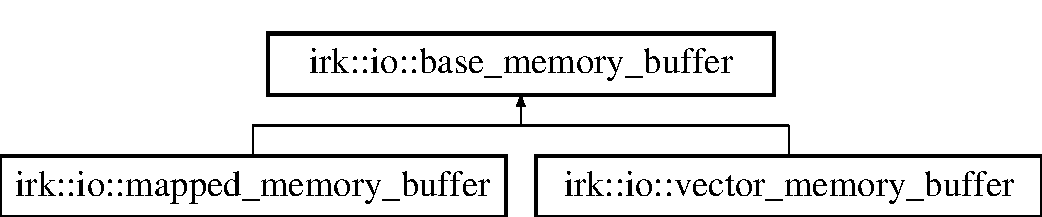
\includegraphics[height=2.000000cm]{classirk_1_1io_1_1base__memory__buffer}
\end{center}
\end{figure}
\subsection*{Public Types}
\begin{DoxyCompactItemize}
\item 
using \mbox{\hyperlink{classirk_1_1io_1_1base__memory__buffer_a1b539180df4274dd4ad0402a0ac821ec}{char\+\_\+type}} = char
\end{DoxyCompactItemize}
\subsection*{Public Member Functions}
\begin{DoxyCompactItemize}
\item 
virtual \mbox{\hyperlink{classirk_1_1io_1_1base__memory__buffer_a1b539180df4274dd4ad0402a0ac821ec}{char\+\_\+type}} $\ast$ \mbox{\hyperlink{classirk_1_1io_1_1base__memory__buffer_ae8247b83aae579cbc04b5432bd4858cc}{data}} ()=0
\item 
virtual const \mbox{\hyperlink{classirk_1_1io_1_1base__memory__buffer_a1b539180df4274dd4ad0402a0ac821ec}{char\+\_\+type}} $\ast$ \mbox{\hyperlink{classirk_1_1io_1_1base__memory__buffer_a87bbff1a6d211e26f0c0aa924a980b9e}{data}} () const =0
\item 
virtual std\+::size\+\_\+t \mbox{\hyperlink{classirk_1_1io_1_1base__memory__buffer_ae634ab934981e7e4baf5e1e67ef3b006}{size}} () const =0
\end{DoxyCompactItemize}


\subsection{Detailed Description}
A base class for all types of memory buffers. 


\begin{DoxyTemplParams}{Template Parameters}
{\em Block} & the underlying type \\
\hline
\end{DoxyTemplParams}
\begin{DoxyAuthor}{Author}
Michal Siedlaczek 
\end{DoxyAuthor}


\subsection{Member Typedef Documentation}
\mbox{\Hypertarget{classirk_1_1io_1_1base__memory__buffer_a1b539180df4274dd4ad0402a0ac821ec}\label{classirk_1_1io_1_1base__memory__buffer_a1b539180df4274dd4ad0402a0ac821ec}} 
\index{irk\+::io\+::base\+\_\+memory\+\_\+buffer@{irk\+::io\+::base\+\_\+memory\+\_\+buffer}!char\+\_\+type@{char\+\_\+type}}
\index{char\+\_\+type@{char\+\_\+type}!irk\+::io\+::base\+\_\+memory\+\_\+buffer@{irk\+::io\+::base\+\_\+memory\+\_\+buffer}}
\subsubsection{\texorpdfstring{char\+\_\+type}{char\_type}}
{\footnotesize\ttfamily using \mbox{\hyperlink{classirk_1_1io_1_1base__memory__buffer_a1b539180df4274dd4ad0402a0ac821ec}{irk\+::io\+::base\+\_\+memory\+\_\+buffer\+::char\+\_\+type}} =  char}



\subsection{Member Function Documentation}
\mbox{\Hypertarget{classirk_1_1io_1_1base__memory__buffer_ae8247b83aae579cbc04b5432bd4858cc}\label{classirk_1_1io_1_1base__memory__buffer_ae8247b83aae579cbc04b5432bd4858cc}} 
\index{irk\+::io\+::base\+\_\+memory\+\_\+buffer@{irk\+::io\+::base\+\_\+memory\+\_\+buffer}!data@{data}}
\index{data@{data}!irk\+::io\+::base\+\_\+memory\+\_\+buffer@{irk\+::io\+::base\+\_\+memory\+\_\+buffer}}
\subsubsection{\texorpdfstring{data()}{data()}\hspace{0.1cm}{\footnotesize\ttfamily [1/2]}}
{\footnotesize\ttfamily virtual \mbox{\hyperlink{classirk_1_1io_1_1base__memory__buffer_a1b539180df4274dd4ad0402a0ac821ec}{char\+\_\+type}}$\ast$ irk\+::io\+::base\+\_\+memory\+\_\+buffer\+::data (\begin{DoxyParamCaption}{ }\end{DoxyParamCaption})\hspace{0.3cm}{\ttfamily [pure virtual]}}



Implemented in \mbox{\hyperlink{classirk_1_1io_1_1mapped__memory__buffer_a2b731cf50320c20fb271bdd5c6f384c4}{irk\+::io\+::mapped\+\_\+memory\+\_\+buffer}}, and \mbox{\hyperlink{classirk_1_1io_1_1vector__memory__buffer_a28ddafbb2610a463d13dc7fe5cf0708f}{irk\+::io\+::vector\+\_\+memory\+\_\+buffer}}.

\mbox{\Hypertarget{classirk_1_1io_1_1base__memory__buffer_a87bbff1a6d211e26f0c0aa924a980b9e}\label{classirk_1_1io_1_1base__memory__buffer_a87bbff1a6d211e26f0c0aa924a980b9e}} 
\index{irk\+::io\+::base\+\_\+memory\+\_\+buffer@{irk\+::io\+::base\+\_\+memory\+\_\+buffer}!data@{data}}
\index{data@{data}!irk\+::io\+::base\+\_\+memory\+\_\+buffer@{irk\+::io\+::base\+\_\+memory\+\_\+buffer}}
\subsubsection{\texorpdfstring{data()}{data()}\hspace{0.1cm}{\footnotesize\ttfamily [2/2]}}
{\footnotesize\ttfamily virtual const \mbox{\hyperlink{classirk_1_1io_1_1base__memory__buffer_a1b539180df4274dd4ad0402a0ac821ec}{char\+\_\+type}}$\ast$ irk\+::io\+::base\+\_\+memory\+\_\+buffer\+::data (\begin{DoxyParamCaption}{ }\end{DoxyParamCaption}) const\hspace{0.3cm}{\ttfamily [pure virtual]}}



Implemented in \mbox{\hyperlink{classirk_1_1io_1_1mapped__memory__buffer_ab4bbb25488358a3d527d45d16a845fb6}{irk\+::io\+::mapped\+\_\+memory\+\_\+buffer}}, and \mbox{\hyperlink{classirk_1_1io_1_1vector__memory__buffer_ad0d18022442c081ac51abb8da8b68e54}{irk\+::io\+::vector\+\_\+memory\+\_\+buffer}}.

\mbox{\Hypertarget{classirk_1_1io_1_1base__memory__buffer_ae634ab934981e7e4baf5e1e67ef3b006}\label{classirk_1_1io_1_1base__memory__buffer_ae634ab934981e7e4baf5e1e67ef3b006}} 
\index{irk\+::io\+::base\+\_\+memory\+\_\+buffer@{irk\+::io\+::base\+\_\+memory\+\_\+buffer}!size@{size}}
\index{size@{size}!irk\+::io\+::base\+\_\+memory\+\_\+buffer@{irk\+::io\+::base\+\_\+memory\+\_\+buffer}}
\subsubsection{\texorpdfstring{size()}{size()}}
{\footnotesize\ttfamily virtual std\+::size\+\_\+t irk\+::io\+::base\+\_\+memory\+\_\+buffer\+::size (\begin{DoxyParamCaption}{ }\end{DoxyParamCaption}) const\hspace{0.3cm}{\ttfamily [pure virtual]}}



Implemented in \mbox{\hyperlink{classirk_1_1io_1_1mapped__memory__buffer_ae64bb8d5018d83bd9feb605704bb0c82}{irk\+::io\+::mapped\+\_\+memory\+\_\+buffer}}, and \mbox{\hyperlink{classirk_1_1io_1_1vector__memory__buffer_ab79eda0d916da980b78ecae09883bba1}{irk\+::io\+::vector\+\_\+memory\+\_\+buffer}}.



The documentation for this class was generated from the following file\+:\begin{DoxyCompactItemize}
\item 
include/irkit/io/\mbox{\hyperlink{memorybuffer_8hpp}{memorybuffer.\+hpp}}\end{DoxyCompactItemize}

\hypertarget{classirk_1_1bitptr}{}\section{irk\+:\+:bitptr$<$ Block $>$ Class Template Reference}
\label{classirk_1_1bitptr}\index{irk\+::bitptr$<$ Block $>$@{irk\+::bitptr$<$ Block $>$}}


A bit pointer class.  




{\ttfamily \#include $<$bitptr.\+hpp$>$}

\subsection*{Classes}
\begin{DoxyCompactItemize}
\item 
struct \mbox{\hyperlink{structirk_1_1bitptr_1_1reader}{reader}}
\end{DoxyCompactItemize}
\subsection*{Public Member Functions}
\begin{DoxyCompactItemize}
\item 
\mbox{\hyperlink{classirk_1_1bitptr_acd28cbb88a0840befdd9bc7a7260f036}{bitptr}} (Block $\ast$block\+\_\+ptr, std\+::uint8\+\_\+t shift=0)
\begin{DoxyCompactList}\small\item\em Creates a pointer to the bit in position {\ttfamily shift} in {\ttfamily block\+\_\+ptr}. \end{DoxyCompactList}\item 
\mbox{\hyperlink{classirk_1_1bitptr_aa1c908a8d26c9286270ccb73ca5a3d85}{bitptr}} (const \mbox{\hyperlink{classirk_1_1bitptr}{bitptr}}$<$ Block $>$ \&other)
\begin{DoxyCompactList}\small\item\em Copy constructor. \end{DoxyCompactList}\item 
void \mbox{\hyperlink{classirk_1_1bitptr_a60b3f1dcb2d6c9f8102c0e077937dcc5}{operator=}} (const \mbox{\hyperlink{classirk_1_1bitptr}{bitptr}}$<$ Block $>$ \&other)
\begin{DoxyCompactList}\small\item\em Assignment operator. \end{DoxyCompactList}\item 
void \mbox{\hyperlink{classirk_1_1bitptr_ab690150f670134eb879fceb83d892073}{set}} (bool bit)
\begin{DoxyCompactList}\small\item\em Sets the bit to the chosen value. \end{DoxyCompactList}\item 
void \mbox{\hyperlink{classirk_1_1bitptr_a11089c343ac361d3ca5d86f8109c2d42}{set}} ()
\begin{DoxyCompactList}\small\item\em Sets the bit to 1. \end{DoxyCompactList}\item 
void \mbox{\hyperlink{classirk_1_1bitptr_acb0f89f9751fc114558234b79d49aac6}{clear}} ()
\begin{DoxyCompactList}\small\item\em Sets the bit to 0. \end{DoxyCompactList}\item 
bit\+\_\+reference \mbox{\hyperlink{classirk_1_1bitptr_a6676fe4fc076f0cb53587ea48d8634c3}{operator$\ast$}} ()
\begin{DoxyCompactList}\small\item\em Returns a non-\/const reference to the bit. \end{DoxyCompactList}\item 
bit\+\_\+reference \mbox{\hyperlink{classirk_1_1bitptr_a1df6b87e20b41de54fd6d582263a905d}{operator\mbox{[}$\,$\mbox{]}}} (int n)
\begin{DoxyCompactList}\small\item\em Returns a non-\/const reference to the {\ttfamily n}-\/th bit. \end{DoxyCompactList}\item 
bool \mbox{\hyperlink{classirk_1_1bitptr_a4cb8f7ff26e561a9348f79082ad6af35}{operator$\ast$}} () const
\begin{DoxyCompactList}\small\item\em Returns the bit value. \end{DoxyCompactList}\item 
bool \mbox{\hyperlink{classirk_1_1bitptr_ae7ed619d650d1982a2510ca8cdd997c1}{operator\mbox{[}$\,$\mbox{]}}} (int n) const
\begin{DoxyCompactList}\small\item\em Returns the value of the {\ttfamily n}-\/th bit. \end{DoxyCompactList}\item 
\mbox{\hyperlink{classirk_1_1bitptr}{bitptr}} \& \mbox{\hyperlink{classirk_1_1bitptr_abb1d7cadd88cb17c9d672a9653d6cbf8}{operator++}} ()
\begin{DoxyCompactList}\small\item\em Increments the pointer to the next bit. \end{DoxyCompactList}\item 
\mbox{\hyperlink{classirk_1_1bitptr}{bitptr}} \mbox{\hyperlink{classirk_1_1bitptr_ad382cd01b956b2b37d62990ca57de170}{operator+}} (int n) const
\begin{DoxyCompactList}\small\item\em Returns a new pointer to the {\ttfamily n}-\/th bit. \end{DoxyCompactList}\item 
\mbox{\hyperlink{classirk_1_1bitptr}{bitptr}} \& \mbox{\hyperlink{classirk_1_1bitptr_a9fcc393a8789c4500391ff3ff2a9fff7}{operator+=}} (int n)
\begin{DoxyCompactList}\small\item\em Increments the pointer by {\ttfamily n} bits. \end{DoxyCompactList}\item 
\mbox{\hyperlink{structirk_1_1bitptr_1_1reader}{reader}} \mbox{\hyperlink{classirk_1_1bitptr_a4505dc024807e2b041ffdc910fae1189}{reader}} ()
\begin{DoxyCompactList}\small\item\em Returns a bit reader starting from the pointer. \end{DoxyCompactList}\end{DoxyCompactItemize}


\subsection{Detailed Description}
\subsubsection*{template$<$class Block$>$\newline
class irk\+::bitptr$<$ Block $>$}

A bit pointer class. 

This class represents a pointer to a particular bit in the underlying data of type {\ttfamily Block}.

Although the behavior is quite similar to regular pointers, there are some fundamental differences.

Note$\ast$$\ast$\+: no decrement or minus operator are defined as of now; therefore, we can only move forward. This will be implemented in the future.


\begin{DoxyTemplParams}{Template Parameters}
{\em Block} & The underlying type. Any bit operations will be performed on a variable of this type. If {\ttfamily sizeof(\+Block) $>$ 1}, then it is on the user to make sure that it does not exceed the bounds. E.\+g., if we create a {\ttfamily bitptr$<$std\+::uint16\+\_\+t$>$(arr)} where {\ttfamily char$\ast$ arr = new char\mbox{[}3\mbox{]}}, there is no way to read bits of the last byte of that array without going out of bounds, because the underlying pointer would be to long. On the other hand, it can be more efficient to use longer types than {\ttfamily char}. Therefore, it is recommended to use whatever type the underlying structure is defined with\+: {\ttfamily char} for {\ttfamily char\mbox{[}\mbox{]}}, {\ttfamily int} for {\ttfamily int\mbox{[}\mbox{]}} and so on. Otherwise, more careful bound checks are required. \\
\hline
\end{DoxyTemplParams}


\subsection{Constructor \& Destructor Documentation}
\mbox{\Hypertarget{classirk_1_1bitptr_acd28cbb88a0840befdd9bc7a7260f036}\label{classirk_1_1bitptr_acd28cbb88a0840befdd9bc7a7260f036}} 
\index{irk\+::bitptr@{irk\+::bitptr}!bitptr@{bitptr}}
\index{bitptr@{bitptr}!irk\+::bitptr@{irk\+::bitptr}}
\subsubsection{\texorpdfstring{bitptr()}{bitptr()}\hspace{0.1cm}{\footnotesize\ttfamily [1/2]}}
{\footnotesize\ttfamily template$<$class Block$>$ \\
\mbox{\hyperlink{classirk_1_1bitptr}{irk\+::bitptr}}$<$ Block $>$\+::\mbox{\hyperlink{classirk_1_1bitptr}{bitptr}} (\begin{DoxyParamCaption}\item[{Block $\ast$}]{block\+\_\+ptr,  }\item[{std\+::uint8\+\_\+t}]{shift = {\ttfamily 0} }\end{DoxyParamCaption})\hspace{0.3cm}{\ttfamily [inline]}}



Creates a pointer to the bit in position {\ttfamily shift} in {\ttfamily block\+\_\+ptr}. 

It is prefectly legal to set {\ttfamily shift $>$ sizeof(\+Block)}; then, it will point to the bit in position {\ttfamily shift \% block\+\_\+bit\+\_\+size} in {\ttfamily block\+\_\+ptr + (shift / block\+\_\+bit\+\_\+size)}.


\begin{DoxyParams}{Parameters}
{\em block\+\_\+ptr} & the created object will point to the least significant bit of this block if {\ttfamily shift = 0} (default) \\
\hline
{\em shift} & the bit offset from the least significant bit of {\ttfamily block\+\_\+ptr}. \\
\hline
\end{DoxyParams}
\mbox{\Hypertarget{classirk_1_1bitptr_aa1c908a8d26c9286270ccb73ca5a3d85}\label{classirk_1_1bitptr_aa1c908a8d26c9286270ccb73ca5a3d85}} 
\index{irk\+::bitptr@{irk\+::bitptr}!bitptr@{bitptr}}
\index{bitptr@{bitptr}!irk\+::bitptr@{irk\+::bitptr}}
\subsubsection{\texorpdfstring{bitptr()}{bitptr()}\hspace{0.1cm}{\footnotesize\ttfamily [2/2]}}
{\footnotesize\ttfamily template$<$class Block$>$ \\
\mbox{\hyperlink{classirk_1_1bitptr}{irk\+::bitptr}}$<$ Block $>$\+::\mbox{\hyperlink{classirk_1_1bitptr}{bitptr}} (\begin{DoxyParamCaption}\item[{const \mbox{\hyperlink{classirk_1_1bitptr}{bitptr}}$<$ Block $>$ \&}]{other }\end{DoxyParamCaption})\hspace{0.3cm}{\ttfamily [inline]}}



Copy constructor. 



\subsection{Member Function Documentation}
\mbox{\Hypertarget{classirk_1_1bitptr_acb0f89f9751fc114558234b79d49aac6}\label{classirk_1_1bitptr_acb0f89f9751fc114558234b79d49aac6}} 
\index{irk\+::bitptr@{irk\+::bitptr}!clear@{clear}}
\index{clear@{clear}!irk\+::bitptr@{irk\+::bitptr}}
\subsubsection{\texorpdfstring{clear()}{clear()}}
{\footnotesize\ttfamily template$<$class Block$>$ \\
void \mbox{\hyperlink{classirk_1_1bitptr}{irk\+::bitptr}}$<$ Block $>$\+::clear (\begin{DoxyParamCaption}{ }\end{DoxyParamCaption})\hspace{0.3cm}{\ttfamily [inline]}}



Sets the bit to 0. 

\mbox{\Hypertarget{classirk_1_1bitptr_a6676fe4fc076f0cb53587ea48d8634c3}\label{classirk_1_1bitptr_a6676fe4fc076f0cb53587ea48d8634c3}} 
\index{irk\+::bitptr@{irk\+::bitptr}!operator$\ast$@{operator$\ast$}}
\index{operator$\ast$@{operator$\ast$}!irk\+::bitptr@{irk\+::bitptr}}
\subsubsection{\texorpdfstring{operator$\ast$()}{operator*()}\hspace{0.1cm}{\footnotesize\ttfamily [1/2]}}
{\footnotesize\ttfamily template$<$class Block$>$ \\
bit\+\_\+reference \mbox{\hyperlink{classirk_1_1bitptr}{irk\+::bitptr}}$<$ Block $>$\+::operator$\ast$ (\begin{DoxyParamCaption}{ }\end{DoxyParamCaption})\hspace{0.3cm}{\ttfamily [inline]}}



Returns a non-\/const reference to the bit. 

It can be later used to assign a value\+: {\ttfamily $\ast$ptr = true}. There is an overhead of creating a proxy reference; therefore, using {\ttfamily \mbox{\hyperlink{classirk_1_1bitptr_ab690150f670134eb879fceb83d892073}{set(bool)}}}, {\ttfamily \mbox{\hyperlink{classirk_1_1bitptr_a11089c343ac361d3ca5d86f8109c2d42}{set()}}} and {\ttfamily \mbox{\hyperlink{classirk_1_1bitptr_acb0f89f9751fc114558234b79d49aac6}{clear()}}} may be more efficient. This operator have been implemented in order to conform to a conventional pointer interface, which might be more generic and interchangable with other interfaces, such as {\ttfamily std\+::vector$<$bool$>$}. \mbox{\Hypertarget{classirk_1_1bitptr_a4cb8f7ff26e561a9348f79082ad6af35}\label{classirk_1_1bitptr_a4cb8f7ff26e561a9348f79082ad6af35}} 
\index{irk\+::bitptr@{irk\+::bitptr}!operator$\ast$@{operator$\ast$}}
\index{operator$\ast$@{operator$\ast$}!irk\+::bitptr@{irk\+::bitptr}}
\subsubsection{\texorpdfstring{operator$\ast$()}{operator*()}\hspace{0.1cm}{\footnotesize\ttfamily [2/2]}}
{\footnotesize\ttfamily template$<$class Block$>$ \\
bool \mbox{\hyperlink{classirk_1_1bitptr}{irk\+::bitptr}}$<$ Block $>$\+::operator$\ast$ (\begin{DoxyParamCaption}{ }\end{DoxyParamCaption}) const\hspace{0.3cm}{\ttfamily [inline]}}



Returns the bit value. 

As opposed to the non-\/const version of this operator, this one does not create a proxy reference. \mbox{\Hypertarget{classirk_1_1bitptr_ad382cd01b956b2b37d62990ca57de170}\label{classirk_1_1bitptr_ad382cd01b956b2b37d62990ca57de170}} 
\index{irk\+::bitptr@{irk\+::bitptr}!operator+@{operator+}}
\index{operator+@{operator+}!irk\+::bitptr@{irk\+::bitptr}}
\subsubsection{\texorpdfstring{operator+()}{operator+()}}
{\footnotesize\ttfamily template$<$class Block$>$ \\
\mbox{\hyperlink{classirk_1_1bitptr}{bitptr}} \mbox{\hyperlink{classirk_1_1bitptr}{irk\+::bitptr}}$<$ Block $>$\+::operator+ (\begin{DoxyParamCaption}\item[{int}]{n }\end{DoxyParamCaption}) const\hspace{0.3cm}{\ttfamily [inline]}}



Returns a new pointer to the {\ttfamily n}-\/th bit. 

\mbox{\Hypertarget{classirk_1_1bitptr_abb1d7cadd88cb17c9d672a9653d6cbf8}\label{classirk_1_1bitptr_abb1d7cadd88cb17c9d672a9653d6cbf8}} 
\index{irk\+::bitptr@{irk\+::bitptr}!operator++@{operator++}}
\index{operator++@{operator++}!irk\+::bitptr@{irk\+::bitptr}}
\subsubsection{\texorpdfstring{operator++()}{operator++()}}
{\footnotesize\ttfamily template$<$class Block$>$ \\
\mbox{\hyperlink{classirk_1_1bitptr}{bitptr}}\& \mbox{\hyperlink{classirk_1_1bitptr}{irk\+::bitptr}}$<$ Block $>$\+::operator++ (\begin{DoxyParamCaption}{ }\end{DoxyParamCaption})\hspace{0.3cm}{\ttfamily [inline]}}



Increments the pointer to the next bit. 

\mbox{\Hypertarget{classirk_1_1bitptr_a9fcc393a8789c4500391ff3ff2a9fff7}\label{classirk_1_1bitptr_a9fcc393a8789c4500391ff3ff2a9fff7}} 
\index{irk\+::bitptr@{irk\+::bitptr}!operator+=@{operator+=}}
\index{operator+=@{operator+=}!irk\+::bitptr@{irk\+::bitptr}}
\subsubsection{\texorpdfstring{operator+=()}{operator+=()}}
{\footnotesize\ttfamily template$<$class Block$>$ \\
\mbox{\hyperlink{classirk_1_1bitptr}{bitptr}}\& \mbox{\hyperlink{classirk_1_1bitptr}{irk\+::bitptr}}$<$ Block $>$\+::operator+= (\begin{DoxyParamCaption}\item[{int}]{n }\end{DoxyParamCaption})\hspace{0.3cm}{\ttfamily [inline]}}



Increments the pointer by {\ttfamily n} bits. 

\mbox{\Hypertarget{classirk_1_1bitptr_a60b3f1dcb2d6c9f8102c0e077937dcc5}\label{classirk_1_1bitptr_a60b3f1dcb2d6c9f8102c0e077937dcc5}} 
\index{irk\+::bitptr@{irk\+::bitptr}!operator=@{operator=}}
\index{operator=@{operator=}!irk\+::bitptr@{irk\+::bitptr}}
\subsubsection{\texorpdfstring{operator=()}{operator=()}}
{\footnotesize\ttfamily template$<$class Block$>$ \\
void \mbox{\hyperlink{classirk_1_1bitptr}{irk\+::bitptr}}$<$ Block $>$\+::operator= (\begin{DoxyParamCaption}\item[{const \mbox{\hyperlink{classirk_1_1bitptr}{bitptr}}$<$ Block $>$ \&}]{other }\end{DoxyParamCaption})\hspace{0.3cm}{\ttfamily [inline]}}



Assignment operator. 

\mbox{\Hypertarget{classirk_1_1bitptr_a1df6b87e20b41de54fd6d582263a905d}\label{classirk_1_1bitptr_a1df6b87e20b41de54fd6d582263a905d}} 
\index{irk\+::bitptr@{irk\+::bitptr}!operator\mbox{[}\mbox{]}@{operator[]}}
\index{operator\mbox{[}\mbox{]}@{operator[]}!irk\+::bitptr@{irk\+::bitptr}}
\subsubsection{\texorpdfstring{operator[]()}{operator[]()}\hspace{0.1cm}{\footnotesize\ttfamily [1/2]}}
{\footnotesize\ttfamily template$<$class Block$>$ \\
bit\+\_\+reference \mbox{\hyperlink{classirk_1_1bitptr}{irk\+::bitptr}}$<$ Block $>$\+::operator\mbox{[}$\,$\mbox{]} (\begin{DoxyParamCaption}\item[{int}]{n }\end{DoxyParamCaption})\hspace{0.3cm}{\ttfamily [inline]}}



Returns a non-\/const reference to the {\ttfamily n}-\/th bit. 

Calling p\mbox{[}n\mbox{]} is equivalent to calling $\ast$(p + n) (see {\ttfamily bit\+\_\+reference \mbox{\hyperlink{classirk_1_1bitptr_a6676fe4fc076f0cb53587ea48d8634c3}{operator$\ast$()}}} documentation). \mbox{\Hypertarget{classirk_1_1bitptr_ae7ed619d650d1982a2510ca8cdd997c1}\label{classirk_1_1bitptr_ae7ed619d650d1982a2510ca8cdd997c1}} 
\index{irk\+::bitptr@{irk\+::bitptr}!operator\mbox{[}\mbox{]}@{operator[]}}
\index{operator\mbox{[}\mbox{]}@{operator[]}!irk\+::bitptr@{irk\+::bitptr}}
\subsubsection{\texorpdfstring{operator[]()}{operator[]()}\hspace{0.1cm}{\footnotesize\ttfamily [2/2]}}
{\footnotesize\ttfamily template$<$class Block$>$ \\
bool \mbox{\hyperlink{classirk_1_1bitptr}{irk\+::bitptr}}$<$ Block $>$\+::operator\mbox{[}$\,$\mbox{]} (\begin{DoxyParamCaption}\item[{int}]{n }\end{DoxyParamCaption}) const\hspace{0.3cm}{\ttfamily [inline]}}



Returns the value of the {\ttfamily n}-\/th bit. 

Calling p\mbox{[}n\mbox{]} is equivalent to calling $\ast$(p + n) (see {\ttfamily bool \mbox{\hyperlink{classirk_1_1bitptr_a6676fe4fc076f0cb53587ea48d8634c3}{operator$\ast$()}}} documentation). \mbox{\Hypertarget{classirk_1_1bitptr_a4505dc024807e2b041ffdc910fae1189}\label{classirk_1_1bitptr_a4505dc024807e2b041ffdc910fae1189}} 
\index{irk\+::bitptr@{irk\+::bitptr}!reader@{reader}}
\index{reader@{reader}!irk\+::bitptr@{irk\+::bitptr}}
\subsubsection{\texorpdfstring{reader()}{reader()}}
{\footnotesize\ttfamily template$<$class Block$>$ \\
\mbox{\hyperlink{structirk_1_1bitptr_1_1reader}{reader}} \mbox{\hyperlink{classirk_1_1bitptr}{irk\+::bitptr}}$<$ Block $>$\+::\mbox{\hyperlink{structirk_1_1bitptr_1_1reader}{reader}} (\begin{DoxyParamCaption}{ }\end{DoxyParamCaption})\hspace{0.3cm}{\ttfamily [inline]}}



Returns a bit reader starting from the pointer. 

\mbox{\Hypertarget{classirk_1_1bitptr_ab690150f670134eb879fceb83d892073}\label{classirk_1_1bitptr_ab690150f670134eb879fceb83d892073}} 
\index{irk\+::bitptr@{irk\+::bitptr}!set@{set}}
\index{set@{set}!irk\+::bitptr@{irk\+::bitptr}}
\subsubsection{\texorpdfstring{set()}{set()}\hspace{0.1cm}{\footnotesize\ttfamily [1/2]}}
{\footnotesize\ttfamily template$<$class Block$>$ \\
void \mbox{\hyperlink{classirk_1_1bitptr}{irk\+::bitptr}}$<$ Block $>$\+::set (\begin{DoxyParamCaption}\item[{bool}]{bit }\end{DoxyParamCaption})\hspace{0.3cm}{\ttfamily [inline]}}



Sets the bit to the chosen value. 


\begin{DoxyParams}{Parameters}
{\em bit} & the value to set the bit to\\
\hline
\end{DoxyParams}
If you can determine {\ttfamily bit} at compile time, you might consider using {\ttfamily \mbox{\hyperlink{classirk_1_1bitptr_a11089c343ac361d3ca5d86f8109c2d42}{set()}}} or {\ttfamily \mbox{\hyperlink{classirk_1_1bitptr_acb0f89f9751fc114558234b79d49aac6}{clear()}}} functions, as they can be slightly more efficient. \mbox{\Hypertarget{classirk_1_1bitptr_a11089c343ac361d3ca5d86f8109c2d42}\label{classirk_1_1bitptr_a11089c343ac361d3ca5d86f8109c2d42}} 
\index{irk\+::bitptr@{irk\+::bitptr}!set@{set}}
\index{set@{set}!irk\+::bitptr@{irk\+::bitptr}}
\subsubsection{\texorpdfstring{set()}{set()}\hspace{0.1cm}{\footnotesize\ttfamily [2/2]}}
{\footnotesize\ttfamily template$<$class Block$>$ \\
void \mbox{\hyperlink{classirk_1_1bitptr}{irk\+::bitptr}}$<$ Block $>$\+::set (\begin{DoxyParamCaption}{ }\end{DoxyParamCaption})\hspace{0.3cm}{\ttfamily [inline]}}



Sets the bit to 1. 



The documentation for this class was generated from the following file\+:\begin{DoxyCompactItemize}
\item 
include/irkit/\mbox{\hyperlink{bitptr_8hpp}{bitptr.\+hpp}}\end{DoxyCompactItemize}

\hypertarget{classirk_1_1prefix__map_1_1block__builder}{}\section{irk\+:\+:prefix\+\_\+map$<$ Index, Memory\+Buffer, Counter $>$\+:\+:block\+\_\+builder Class Reference}
\label{classirk_1_1prefix__map_1_1block__builder}\index{irk\+::prefix\+\_\+map$<$ Index, Memory\+Buffer, Counter $>$\+::block\+\_\+builder@{irk\+::prefix\+\_\+map$<$ Index, Memory\+Buffer, Counter $>$\+::block\+\_\+builder}}


{\ttfamily \#include $<$prefixmap.\+hpp$>$}

\subsection*{Public Member Functions}
\begin{DoxyCompactItemize}
\item 
\mbox{\hyperlink{classirk_1_1prefix__map_1_1block__builder_af6ed7104994775956eb88348b87c46d8}{block\+\_\+builder}} (Index first\+\_\+index, char $\ast$block\+\_\+begin, std\+::size\+\_\+t \mbox{\hyperlink{classirk_1_1prefix__map_1_1block__builder_ac3fb0a31f627e1f49b9eb0738742dd23}{size}}, const std\+::shared\+\_\+ptr$<$ \mbox{\hyperlink{classirk_1_1hutucker__codec}{hutucker\+\_\+codec}}$<$ char $>$$>$ codec)
\item 
bool \mbox{\hyperlink{classirk_1_1prefix__map_1_1block__builder_a7624581bf15668f0be6733f8105d4c59}{add}} (const std\+::string \&value)
\item 
void \mbox{\hyperlink{classirk_1_1prefix__map_1_1block__builder_a86b281aeb689345c5cac4b3a9266d3a6}{expand\+\_\+by}} (std\+::size\+\_\+t \mbox{\hyperlink{namespaceirk_a655971fe9a3706528f14c395f938d416}{nbytes}})
\item 
void \mbox{\hyperlink{classirk_1_1prefix__map_1_1block__builder_aa25610a99626d90e1b3232fc05fe58cb}{reset}} (char $\ast$new\+\_\+begin)
\item 
auto \mbox{\hyperlink{classirk_1_1prefix__map_1_1block__builder_ac3fb0a31f627e1f49b9eb0738742dd23}{size}} () const
\item 
void \mbox{\hyperlink{classirk_1_1prefix__map_1_1block__builder_acd19257e8bac2d4af07431383c1c2c16}{write\+\_\+count}} ()
\item 
void \mbox{\hyperlink{classirk_1_1prefix__map_1_1block__builder_ac2b76fd0236effde8936f1d710b29aed}{close}} ()
\end{DoxyCompactItemize}


\subsection{Detailed Description}
\subsubsection*{template$<$class Index, class Memory\+Buffer, class Counter = std\+::uint32\+\_\+t$>$\newline
class irk\+::prefix\+\_\+map$<$ Index, Memory\+Buffer, Counter $>$\+::block\+\_\+builder}

An object of this class is responsible for building a single compressed block of a prefix map. 

\subsection{Constructor \& Destructor Documentation}
\mbox{\Hypertarget{classirk_1_1prefix__map_1_1block__builder_af6ed7104994775956eb88348b87c46d8}\label{classirk_1_1prefix__map_1_1block__builder_af6ed7104994775956eb88348b87c46d8}} 
\index{irk\+::prefix\+\_\+map\+::block\+\_\+builder@{irk\+::prefix\+\_\+map\+::block\+\_\+builder}!block\+\_\+builder@{block\+\_\+builder}}
\index{block\+\_\+builder@{block\+\_\+builder}!irk\+::prefix\+\_\+map\+::block\+\_\+builder@{irk\+::prefix\+\_\+map\+::block\+\_\+builder}}
\subsubsection{\texorpdfstring{block\+\_\+builder()}{block\_builder()}}
{\footnotesize\ttfamily template$<$class Index, class Memory\+Buffer, class Counter = std\+::uint32\+\_\+t$>$ \\
\mbox{\hyperlink{classirk_1_1prefix__map}{irk\+::prefix\+\_\+map}}$<$ Index, Memory\+Buffer, Counter $>$\+::block\+\_\+builder\+::block\+\_\+builder (\begin{DoxyParamCaption}\item[{Index}]{first\+\_\+index,  }\item[{char $\ast$}]{block\+\_\+begin,  }\item[{std\+::size\+\_\+t}]{size,  }\item[{const std\+::shared\+\_\+ptr$<$ \mbox{\hyperlink{classirk_1_1hutucker__codec}{hutucker\+\_\+codec}}$<$ char $>$$>$}]{codec }\end{DoxyParamCaption})\hspace{0.3cm}{\ttfamily [inline]}}



\subsection{Member Function Documentation}
\mbox{\Hypertarget{classirk_1_1prefix__map_1_1block__builder_a7624581bf15668f0be6733f8105d4c59}\label{classirk_1_1prefix__map_1_1block__builder_a7624581bf15668f0be6733f8105d4c59}} 
\index{irk\+::prefix\+\_\+map\+::block\+\_\+builder@{irk\+::prefix\+\_\+map\+::block\+\_\+builder}!add@{add}}
\index{add@{add}!irk\+::prefix\+\_\+map\+::block\+\_\+builder@{irk\+::prefix\+\_\+map\+::block\+\_\+builder}}
\subsubsection{\texorpdfstring{add()}{add()}}
{\footnotesize\ttfamily template$<$class Index, class Memory\+Buffer, class Counter = std\+::uint32\+\_\+t$>$ \\
bool \mbox{\hyperlink{classirk_1_1prefix__map}{irk\+::prefix\+\_\+map}}$<$ Index, Memory\+Buffer, Counter $>$\+::block\+\_\+builder\+::add (\begin{DoxyParamCaption}\item[{const std\+::string \&}]{value }\end{DoxyParamCaption})\hspace{0.3cm}{\ttfamily [inline]}}

\mbox{\Hypertarget{classirk_1_1prefix__map_1_1block__builder_ac2b76fd0236effde8936f1d710b29aed}\label{classirk_1_1prefix__map_1_1block__builder_ac2b76fd0236effde8936f1d710b29aed}} 
\index{irk\+::prefix\+\_\+map\+::block\+\_\+builder@{irk\+::prefix\+\_\+map\+::block\+\_\+builder}!close@{close}}
\index{close@{close}!irk\+::prefix\+\_\+map\+::block\+\_\+builder@{irk\+::prefix\+\_\+map\+::block\+\_\+builder}}
\subsubsection{\texorpdfstring{close()}{close()}}
{\footnotesize\ttfamily template$<$class Index, class Memory\+Buffer, class Counter = std\+::uint32\+\_\+t$>$ \\
void \mbox{\hyperlink{classirk_1_1prefix__map}{irk\+::prefix\+\_\+map}}$<$ Index, Memory\+Buffer, Counter $>$\+::block\+\_\+builder\+::close (\begin{DoxyParamCaption}{ }\end{DoxyParamCaption})\hspace{0.3cm}{\ttfamily [inline]}}

\mbox{\Hypertarget{classirk_1_1prefix__map_1_1block__builder_a86b281aeb689345c5cac4b3a9266d3a6}\label{classirk_1_1prefix__map_1_1block__builder_a86b281aeb689345c5cac4b3a9266d3a6}} 
\index{irk\+::prefix\+\_\+map\+::block\+\_\+builder@{irk\+::prefix\+\_\+map\+::block\+\_\+builder}!expand\+\_\+by@{expand\+\_\+by}}
\index{expand\+\_\+by@{expand\+\_\+by}!irk\+::prefix\+\_\+map\+::block\+\_\+builder@{irk\+::prefix\+\_\+map\+::block\+\_\+builder}}
\subsubsection{\texorpdfstring{expand\+\_\+by()}{expand\_by()}}
{\footnotesize\ttfamily template$<$class Index, class Memory\+Buffer, class Counter = std\+::uint32\+\_\+t$>$ \\
void \mbox{\hyperlink{classirk_1_1prefix__map}{irk\+::prefix\+\_\+map}}$<$ Index, Memory\+Buffer, Counter $>$\+::block\+\_\+builder\+::expand\+\_\+by (\begin{DoxyParamCaption}\item[{std\+::size\+\_\+t}]{nbytes }\end{DoxyParamCaption})\hspace{0.3cm}{\ttfamily [inline]}}

\mbox{\Hypertarget{classirk_1_1prefix__map_1_1block__builder_aa25610a99626d90e1b3232fc05fe58cb}\label{classirk_1_1prefix__map_1_1block__builder_aa25610a99626d90e1b3232fc05fe58cb}} 
\index{irk\+::prefix\+\_\+map\+::block\+\_\+builder@{irk\+::prefix\+\_\+map\+::block\+\_\+builder}!reset@{reset}}
\index{reset@{reset}!irk\+::prefix\+\_\+map\+::block\+\_\+builder@{irk\+::prefix\+\_\+map\+::block\+\_\+builder}}
\subsubsection{\texorpdfstring{reset()}{reset()}}
{\footnotesize\ttfamily template$<$class Index, class Memory\+Buffer, class Counter = std\+::uint32\+\_\+t$>$ \\
void \mbox{\hyperlink{classirk_1_1prefix__map}{irk\+::prefix\+\_\+map}}$<$ Index, Memory\+Buffer, Counter $>$\+::block\+\_\+builder\+::reset (\begin{DoxyParamCaption}\item[{char $\ast$}]{new\+\_\+begin }\end{DoxyParamCaption})\hspace{0.3cm}{\ttfamily [inline]}}

\mbox{\Hypertarget{classirk_1_1prefix__map_1_1block__builder_ac3fb0a31f627e1f49b9eb0738742dd23}\label{classirk_1_1prefix__map_1_1block__builder_ac3fb0a31f627e1f49b9eb0738742dd23}} 
\index{irk\+::prefix\+\_\+map\+::block\+\_\+builder@{irk\+::prefix\+\_\+map\+::block\+\_\+builder}!size@{size}}
\index{size@{size}!irk\+::prefix\+\_\+map\+::block\+\_\+builder@{irk\+::prefix\+\_\+map\+::block\+\_\+builder}}
\subsubsection{\texorpdfstring{size()}{size()}}
{\footnotesize\ttfamily template$<$class Index, class Memory\+Buffer, class Counter = std\+::uint32\+\_\+t$>$ \\
auto \mbox{\hyperlink{classirk_1_1prefix__map}{irk\+::prefix\+\_\+map}}$<$ Index, Memory\+Buffer, Counter $>$\+::block\+\_\+builder\+::size (\begin{DoxyParamCaption}{ }\end{DoxyParamCaption}) const\hspace{0.3cm}{\ttfamily [inline]}}

\mbox{\Hypertarget{classirk_1_1prefix__map_1_1block__builder_acd19257e8bac2d4af07431383c1c2c16}\label{classirk_1_1prefix__map_1_1block__builder_acd19257e8bac2d4af07431383c1c2c16}} 
\index{irk\+::prefix\+\_\+map\+::block\+\_\+builder@{irk\+::prefix\+\_\+map\+::block\+\_\+builder}!write\+\_\+count@{write\+\_\+count}}
\index{write\+\_\+count@{write\+\_\+count}!irk\+::prefix\+\_\+map\+::block\+\_\+builder@{irk\+::prefix\+\_\+map\+::block\+\_\+builder}}
\subsubsection{\texorpdfstring{write\+\_\+count()}{write\_count()}}
{\footnotesize\ttfamily template$<$class Index, class Memory\+Buffer, class Counter = std\+::uint32\+\_\+t$>$ \\
void \mbox{\hyperlink{classirk_1_1prefix__map}{irk\+::prefix\+\_\+map}}$<$ Index, Memory\+Buffer, Counter $>$\+::block\+\_\+builder\+::write\+\_\+count (\begin{DoxyParamCaption}{ }\end{DoxyParamCaption})\hspace{0.3cm}{\ttfamily [inline]}}



The documentation for this class was generated from the following file\+:\begin{DoxyCompactItemize}
\item 
include/irkit/\mbox{\hyperlink{prefixmap_8hpp}{prefixmap.\+hpp}}\end{DoxyCompactItemize}

\hypertarget{classirk_1_1index_1_1block__document__list__view}{}\section{irk\+:\+:index\+:\+:block\+\_\+document\+\_\+list\+\_\+view$<$ Codec $>$ Class Template Reference}
\label{classirk_1_1index_1_1block__document__list__view}\index{irk\+::index\+::block\+\_\+document\+\_\+list\+\_\+view$<$ Codec $>$@{irk\+::index\+::block\+\_\+document\+\_\+list\+\_\+view$<$ Codec $>$}}


A view of a block document list.  




{\ttfamily \#include $<$block\+\_\+inverted\+\_\+list.\+hpp$>$}

\subsection*{Public Types}
\begin{DoxyCompactItemize}
\item 
using \mbox{\hyperlink{classirk_1_1index_1_1block__document__list__view_abc1e76d262386112c4591362fc660dda}{size\+\_\+type}} = int32\+\_\+t
\item 
using \mbox{\hyperlink{classirk_1_1index_1_1block__document__list__view_a06e2f36c5850de123fefa071ae56da92}{value\+\_\+type}} = \mbox{\hyperlink{namespaceirk_1_1index_af829dedea20da89f9b51b49d78f57006}{document\+\_\+t}}
\item 
using \mbox{\hyperlink{classirk_1_1index_1_1block__document__list__view_aaf5438363796f98a08a115e2a6316659}{self\+\_\+type}} = \mbox{\hyperlink{classirk_1_1index_1_1block__document__list__view}{block\+\_\+document\+\_\+list\+\_\+view}}
\item 
using \mbox{\hyperlink{classirk_1_1index_1_1block__document__list__view_afc4738502c6c0b43f8487be16136feec}{iterator}} = \mbox{\hyperlink{classirk_1_1index_1_1block__iterator}{block\+\_\+iterator}}$<$ \mbox{\hyperlink{classirk_1_1index_1_1block__document__list__view_aaf5438363796f98a08a115e2a6316659}{self\+\_\+type}}, true $>$
\item 
using \mbox{\hyperlink{classirk_1_1index_1_1block__document__list__view_ac08980dc0eeb9fea5528fb110a2ce734}{codec\+\_\+type}} = Codec
\end{DoxyCompactItemize}
\subsection*{Public Member Functions}
\begin{DoxyCompactItemize}
\item 
\mbox{\hyperlink{classirk_1_1index_1_1block__document__list__view_a9664030e51525833bbe188c0ffaf763e}{block\+\_\+document\+\_\+list\+\_\+view}} ()=default
\item 
\mbox{\hyperlink{classirk_1_1index_1_1block__document__list__view_a7618502e688a818d719a9bc939753390}{block\+\_\+document\+\_\+list\+\_\+view}} (\mbox{\hyperlink{classirk_1_1memory__view}{irk\+::memory\+\_\+view}} mem, int32\+\_\+t length)
\begin{DoxyCompactList}\small\item\em Constructs the view. \end{DoxyCompactList}\item 
\mbox{\hyperlink{classirk_1_1index_1_1block__document__list__view_afc4738502c6c0b43f8487be16136feec}{iterator}} \mbox{\hyperlink{classirk_1_1index_1_1block__document__list__view_a940c6d0b71559861f737e4cf83967d89}{begin}} () const
\item 
\mbox{\hyperlink{classirk_1_1index_1_1block__document__list__view_afc4738502c6c0b43f8487be16136feec}{iterator}} \mbox{\hyperlink{classirk_1_1index_1_1block__document__list__view_a436a88ad1c67c712c6b0aee63d28d1e4}{end}} () const
\item 
\mbox{\hyperlink{classirk_1_1index_1_1block__document__list__view_afc4738502c6c0b43f8487be16136feec}{iterator}} \mbox{\hyperlink{classirk_1_1index_1_1block__document__list__view_a5b34a202589c619eb9e2aec9043dfd02}{lookup}} (\mbox{\hyperlink{classirk_1_1index_1_1block__document__list__view_a06e2f36c5850de123fefa071ae56da92}{value\+\_\+type}} id) const
\begin{DoxyCompactList}\small\item\em Finds the position of {\ttfamily id} or the next greater. \end{DoxyCompactList}\item 
int32\+\_\+t \mbox{\hyperlink{classirk_1_1index_1_1block__document__list__view_ad54848af1d979186618564f0cb7dd598}{size}} () const
\item 
int64\+\_\+t \mbox{\hyperlink{classirk_1_1index_1_1block__document__list__view_a5d2794987db8ca0a090ffdf1cc6c235f}{memory\+\_\+size}} () const
\item 
\mbox{\hyperlink{classirk_1_1memory__view}{memory\+\_\+view}} \mbox{\hyperlink{classirk_1_1index_1_1block__document__list__view_a05d9aaf476ec8dc2a5077e5d549b8915}{memory}} () const
\item 
std\+::ostream \& \mbox{\hyperlink{classirk_1_1index_1_1block__document__list__view_a2e535fb377bac8f0332add83017eec01}{write}} (std\+::ostream \&out) const
\end{DoxyCompactItemize}
\subsection*{Friends}
\begin{DoxyCompactItemize}
\item 
class \mbox{\hyperlink{classirk_1_1index_1_1block__document__list__view_a9e9d706e71ebb8b3d20137fb0121c8bd}{block\+\_\+iterator$<$ self\+\_\+type, true $>$}}
\end{DoxyCompactItemize}


\subsection{Detailed Description}
\subsubsection*{template$<$class Codec$>$\newline
class irk\+::index\+::block\+\_\+document\+\_\+list\+\_\+view$<$ Codec $>$}

A view of a block document list. 


\begin{DoxyTemplParams}{Template Parameters}
{\em Doc} & type of document ID, must be integer. \\
\hline
\end{DoxyTemplParams}


\subsection{Member Typedef Documentation}
\mbox{\Hypertarget{classirk_1_1index_1_1block__document__list__view_ac08980dc0eeb9fea5528fb110a2ce734}\label{classirk_1_1index_1_1block__document__list__view_ac08980dc0eeb9fea5528fb110a2ce734}} 
\index{irk\+::index\+::block\+\_\+document\+\_\+list\+\_\+view@{irk\+::index\+::block\+\_\+document\+\_\+list\+\_\+view}!codec\+\_\+type@{codec\+\_\+type}}
\index{codec\+\_\+type@{codec\+\_\+type}!irk\+::index\+::block\+\_\+document\+\_\+list\+\_\+view@{irk\+::index\+::block\+\_\+document\+\_\+list\+\_\+view}}
\subsubsection{\texorpdfstring{codec\+\_\+type}{codec\_type}}
{\footnotesize\ttfamily template$<$class Codec$>$ \\
using \mbox{\hyperlink{classirk_1_1index_1_1block__document__list__view}{irk\+::index\+::block\+\_\+document\+\_\+list\+\_\+view}}$<$ Codec $>$\+::\mbox{\hyperlink{classirk_1_1index_1_1block__document__list__view_ac08980dc0eeb9fea5528fb110a2ce734}{codec\+\_\+type}} =  Codec}

\mbox{\Hypertarget{classirk_1_1index_1_1block__document__list__view_afc4738502c6c0b43f8487be16136feec}\label{classirk_1_1index_1_1block__document__list__view_afc4738502c6c0b43f8487be16136feec}} 
\index{irk\+::index\+::block\+\_\+document\+\_\+list\+\_\+view@{irk\+::index\+::block\+\_\+document\+\_\+list\+\_\+view}!iterator@{iterator}}
\index{iterator@{iterator}!irk\+::index\+::block\+\_\+document\+\_\+list\+\_\+view@{irk\+::index\+::block\+\_\+document\+\_\+list\+\_\+view}}
\subsubsection{\texorpdfstring{iterator}{iterator}}
{\footnotesize\ttfamily template$<$class Codec$>$ \\
using \mbox{\hyperlink{classirk_1_1index_1_1block__document__list__view}{irk\+::index\+::block\+\_\+document\+\_\+list\+\_\+view}}$<$ Codec $>$\+::\mbox{\hyperlink{classirk_1_1index_1_1block__document__list__view_afc4738502c6c0b43f8487be16136feec}{iterator}} =  \mbox{\hyperlink{classirk_1_1index_1_1block__iterator}{block\+\_\+iterator}}$<$\mbox{\hyperlink{classirk_1_1index_1_1block__document__list__view_aaf5438363796f98a08a115e2a6316659}{self\+\_\+type}}, true$>$}

\mbox{\Hypertarget{classirk_1_1index_1_1block__document__list__view_aaf5438363796f98a08a115e2a6316659}\label{classirk_1_1index_1_1block__document__list__view_aaf5438363796f98a08a115e2a6316659}} 
\index{irk\+::index\+::block\+\_\+document\+\_\+list\+\_\+view@{irk\+::index\+::block\+\_\+document\+\_\+list\+\_\+view}!self\+\_\+type@{self\+\_\+type}}
\index{self\+\_\+type@{self\+\_\+type}!irk\+::index\+::block\+\_\+document\+\_\+list\+\_\+view@{irk\+::index\+::block\+\_\+document\+\_\+list\+\_\+view}}
\subsubsection{\texorpdfstring{self\+\_\+type}{self\_type}}
{\footnotesize\ttfamily template$<$class Codec$>$ \\
using \mbox{\hyperlink{classirk_1_1index_1_1block__document__list__view}{irk\+::index\+::block\+\_\+document\+\_\+list\+\_\+view}}$<$ Codec $>$\+::\mbox{\hyperlink{classirk_1_1index_1_1block__document__list__view_aaf5438363796f98a08a115e2a6316659}{self\+\_\+type}} =  \mbox{\hyperlink{classirk_1_1index_1_1block__document__list__view}{block\+\_\+document\+\_\+list\+\_\+view}}}

\mbox{\Hypertarget{classirk_1_1index_1_1block__document__list__view_abc1e76d262386112c4591362fc660dda}\label{classirk_1_1index_1_1block__document__list__view_abc1e76d262386112c4591362fc660dda}} 
\index{irk\+::index\+::block\+\_\+document\+\_\+list\+\_\+view@{irk\+::index\+::block\+\_\+document\+\_\+list\+\_\+view}!size\+\_\+type@{size\+\_\+type}}
\index{size\+\_\+type@{size\+\_\+type}!irk\+::index\+::block\+\_\+document\+\_\+list\+\_\+view@{irk\+::index\+::block\+\_\+document\+\_\+list\+\_\+view}}
\subsubsection{\texorpdfstring{size\+\_\+type}{size\_type}}
{\footnotesize\ttfamily template$<$class Codec$>$ \\
using \mbox{\hyperlink{classirk_1_1index_1_1block__document__list__view}{irk\+::index\+::block\+\_\+document\+\_\+list\+\_\+view}}$<$ Codec $>$\+::\mbox{\hyperlink{classirk_1_1index_1_1block__document__list__view_abc1e76d262386112c4591362fc660dda}{size\+\_\+type}} =  int32\+\_\+t}

\mbox{\Hypertarget{classirk_1_1index_1_1block__document__list__view_a06e2f36c5850de123fefa071ae56da92}\label{classirk_1_1index_1_1block__document__list__view_a06e2f36c5850de123fefa071ae56da92}} 
\index{irk\+::index\+::block\+\_\+document\+\_\+list\+\_\+view@{irk\+::index\+::block\+\_\+document\+\_\+list\+\_\+view}!value\+\_\+type@{value\+\_\+type}}
\index{value\+\_\+type@{value\+\_\+type}!irk\+::index\+::block\+\_\+document\+\_\+list\+\_\+view@{irk\+::index\+::block\+\_\+document\+\_\+list\+\_\+view}}
\subsubsection{\texorpdfstring{value\+\_\+type}{value\_type}}
{\footnotesize\ttfamily template$<$class Codec$>$ \\
using \mbox{\hyperlink{classirk_1_1index_1_1block__document__list__view}{irk\+::index\+::block\+\_\+document\+\_\+list\+\_\+view}}$<$ Codec $>$\+::\mbox{\hyperlink{classirk_1_1index_1_1block__document__list__view_a06e2f36c5850de123fefa071ae56da92}{value\+\_\+type}} =  \mbox{\hyperlink{namespaceirk_1_1index_af829dedea20da89f9b51b49d78f57006}{document\+\_\+t}}}



\subsection{Constructor \& Destructor Documentation}
\mbox{\Hypertarget{classirk_1_1index_1_1block__document__list__view_a9664030e51525833bbe188c0ffaf763e}\label{classirk_1_1index_1_1block__document__list__view_a9664030e51525833bbe188c0ffaf763e}} 
\index{irk\+::index\+::block\+\_\+document\+\_\+list\+\_\+view@{irk\+::index\+::block\+\_\+document\+\_\+list\+\_\+view}!block\+\_\+document\+\_\+list\+\_\+view@{block\+\_\+document\+\_\+list\+\_\+view}}
\index{block\+\_\+document\+\_\+list\+\_\+view@{block\+\_\+document\+\_\+list\+\_\+view}!irk\+::index\+::block\+\_\+document\+\_\+list\+\_\+view@{irk\+::index\+::block\+\_\+document\+\_\+list\+\_\+view}}
\subsubsection{\texorpdfstring{block\+\_\+document\+\_\+list\+\_\+view()}{block\_document\_list\_view()}\hspace{0.1cm}{\footnotesize\ttfamily [1/2]}}
{\footnotesize\ttfamily template$<$class Codec$>$ \\
\mbox{\hyperlink{classirk_1_1index_1_1block__document__list__view}{irk\+::index\+::block\+\_\+document\+\_\+list\+\_\+view}}$<$ Codec $>$\+::\mbox{\hyperlink{classirk_1_1index_1_1block__document__list__view}{block\+\_\+document\+\_\+list\+\_\+view}} (\begin{DoxyParamCaption}{ }\end{DoxyParamCaption})\hspace{0.3cm}{\ttfamily [default]}}

\mbox{\Hypertarget{classirk_1_1index_1_1block__document__list__view_a7618502e688a818d719a9bc939753390}\label{classirk_1_1index_1_1block__document__list__view_a7618502e688a818d719a9bc939753390}} 
\index{irk\+::index\+::block\+\_\+document\+\_\+list\+\_\+view@{irk\+::index\+::block\+\_\+document\+\_\+list\+\_\+view}!block\+\_\+document\+\_\+list\+\_\+view@{block\+\_\+document\+\_\+list\+\_\+view}}
\index{block\+\_\+document\+\_\+list\+\_\+view@{block\+\_\+document\+\_\+list\+\_\+view}!irk\+::index\+::block\+\_\+document\+\_\+list\+\_\+view@{irk\+::index\+::block\+\_\+document\+\_\+list\+\_\+view}}
\subsubsection{\texorpdfstring{block\+\_\+document\+\_\+list\+\_\+view()}{block\_document\_list\_view()}\hspace{0.1cm}{\footnotesize\ttfamily [2/2]}}
{\footnotesize\ttfamily template$<$class Codec$>$ \\
\mbox{\hyperlink{classirk_1_1index_1_1block__document__list__view}{irk\+::index\+::block\+\_\+document\+\_\+list\+\_\+view}}$<$ Codec $>$\+::\mbox{\hyperlink{classirk_1_1index_1_1block__document__list__view}{block\+\_\+document\+\_\+list\+\_\+view}} (\begin{DoxyParamCaption}\item[{\mbox{\hyperlink{classirk_1_1memory__view}{irk\+::memory\+\_\+view}}}]{mem,  }\item[{int32\+\_\+t}]{length }\end{DoxyParamCaption})\hspace{0.3cm}{\ttfamily [inline]}}



Constructs the view. 


\begin{DoxyParams}{Parameters}
{\em doc\+\_\+codec} & a codec for document I\+Ds \\
\hline
{\em mem} & a memory view containing the list \\
\hline
{\em length} & the number of elements in the list \\
\hline
{\em offset} & offset from the beginning of {\ttfamily mem} \\
\hline
\end{DoxyParams}


\subsection{Member Function Documentation}
\mbox{\Hypertarget{classirk_1_1index_1_1block__document__list__view_a940c6d0b71559861f737e4cf83967d89}\label{classirk_1_1index_1_1block__document__list__view_a940c6d0b71559861f737e4cf83967d89}} 
\index{irk\+::index\+::block\+\_\+document\+\_\+list\+\_\+view@{irk\+::index\+::block\+\_\+document\+\_\+list\+\_\+view}!begin@{begin}}
\index{begin@{begin}!irk\+::index\+::block\+\_\+document\+\_\+list\+\_\+view@{irk\+::index\+::block\+\_\+document\+\_\+list\+\_\+view}}
\subsubsection{\texorpdfstring{begin()}{begin()}}
{\footnotesize\ttfamily template$<$class Codec$>$ \\
\mbox{\hyperlink{classirk_1_1index_1_1block__document__list__view_afc4738502c6c0b43f8487be16136feec}{iterator}} \mbox{\hyperlink{classirk_1_1index_1_1block__document__list__view}{irk\+::index\+::block\+\_\+document\+\_\+list\+\_\+view}}$<$ Codec $>$\+::begin (\begin{DoxyParamCaption}{ }\end{DoxyParamCaption}) const\hspace{0.3cm}{\ttfamily [inline]}}

\mbox{\Hypertarget{classirk_1_1index_1_1block__document__list__view_a436a88ad1c67c712c6b0aee63d28d1e4}\label{classirk_1_1index_1_1block__document__list__view_a436a88ad1c67c712c6b0aee63d28d1e4}} 
\index{irk\+::index\+::block\+\_\+document\+\_\+list\+\_\+view@{irk\+::index\+::block\+\_\+document\+\_\+list\+\_\+view}!end@{end}}
\index{end@{end}!irk\+::index\+::block\+\_\+document\+\_\+list\+\_\+view@{irk\+::index\+::block\+\_\+document\+\_\+list\+\_\+view}}
\subsubsection{\texorpdfstring{end()}{end()}}
{\footnotesize\ttfamily template$<$class Codec$>$ \\
\mbox{\hyperlink{classirk_1_1index_1_1block__document__list__view_afc4738502c6c0b43f8487be16136feec}{iterator}} \mbox{\hyperlink{classirk_1_1index_1_1block__document__list__view}{irk\+::index\+::block\+\_\+document\+\_\+list\+\_\+view}}$<$ Codec $>$\+::end (\begin{DoxyParamCaption}{ }\end{DoxyParamCaption}) const\hspace{0.3cm}{\ttfamily [inline]}}

\mbox{\Hypertarget{classirk_1_1index_1_1block__document__list__view_a5b34a202589c619eb9e2aec9043dfd02}\label{classirk_1_1index_1_1block__document__list__view_a5b34a202589c619eb9e2aec9043dfd02}} 
\index{irk\+::index\+::block\+\_\+document\+\_\+list\+\_\+view@{irk\+::index\+::block\+\_\+document\+\_\+list\+\_\+view}!lookup@{lookup}}
\index{lookup@{lookup}!irk\+::index\+::block\+\_\+document\+\_\+list\+\_\+view@{irk\+::index\+::block\+\_\+document\+\_\+list\+\_\+view}}
\subsubsection{\texorpdfstring{lookup()}{lookup()}}
{\footnotesize\ttfamily template$<$class Codec$>$ \\
\mbox{\hyperlink{classirk_1_1index_1_1block__document__list__view_afc4738502c6c0b43f8487be16136feec}{iterator}} \mbox{\hyperlink{classirk_1_1index_1_1block__document__list__view}{irk\+::index\+::block\+\_\+document\+\_\+list\+\_\+view}}$<$ Codec $>$\+::lookup (\begin{DoxyParamCaption}\item[{\mbox{\hyperlink{classirk_1_1index_1_1block__document__list__view_a06e2f36c5850de123fefa071ae56da92}{value\+\_\+type}}}]{id }\end{DoxyParamCaption}) const\hspace{0.3cm}{\ttfamily [inline]}}



Finds the position of {\ttfamily id} or the next greater. 

\mbox{\Hypertarget{classirk_1_1index_1_1block__document__list__view_a05d9aaf476ec8dc2a5077e5d549b8915}\label{classirk_1_1index_1_1block__document__list__view_a05d9aaf476ec8dc2a5077e5d549b8915}} 
\index{irk\+::index\+::block\+\_\+document\+\_\+list\+\_\+view@{irk\+::index\+::block\+\_\+document\+\_\+list\+\_\+view}!memory@{memory}}
\index{memory@{memory}!irk\+::index\+::block\+\_\+document\+\_\+list\+\_\+view@{irk\+::index\+::block\+\_\+document\+\_\+list\+\_\+view}}
\subsubsection{\texorpdfstring{memory()}{memory()}}
{\footnotesize\ttfamily template$<$class Codec$>$ \\
\mbox{\hyperlink{classirk_1_1memory__view}{memory\+\_\+view}} \mbox{\hyperlink{classirk_1_1index_1_1block__document__list__view}{irk\+::index\+::block\+\_\+document\+\_\+list\+\_\+view}}$<$ Codec $>$\+::memory (\begin{DoxyParamCaption}{ }\end{DoxyParamCaption}) const\hspace{0.3cm}{\ttfamily [inline]}}

\mbox{\Hypertarget{classirk_1_1index_1_1block__document__list__view_a5d2794987db8ca0a090ffdf1cc6c235f}\label{classirk_1_1index_1_1block__document__list__view_a5d2794987db8ca0a090ffdf1cc6c235f}} 
\index{irk\+::index\+::block\+\_\+document\+\_\+list\+\_\+view@{irk\+::index\+::block\+\_\+document\+\_\+list\+\_\+view}!memory\+\_\+size@{memory\+\_\+size}}
\index{memory\+\_\+size@{memory\+\_\+size}!irk\+::index\+::block\+\_\+document\+\_\+list\+\_\+view@{irk\+::index\+::block\+\_\+document\+\_\+list\+\_\+view}}
\subsubsection{\texorpdfstring{memory\+\_\+size()}{memory\_size()}}
{\footnotesize\ttfamily template$<$class Codec$>$ \\
int64\+\_\+t \mbox{\hyperlink{classirk_1_1index_1_1block__document__list__view}{irk\+::index\+::block\+\_\+document\+\_\+list\+\_\+view}}$<$ Codec $>$\+::memory\+\_\+size (\begin{DoxyParamCaption}{ }\end{DoxyParamCaption}) const\hspace{0.3cm}{\ttfamily [inline]}}

\mbox{\Hypertarget{classirk_1_1index_1_1block__document__list__view_ad54848af1d979186618564f0cb7dd598}\label{classirk_1_1index_1_1block__document__list__view_ad54848af1d979186618564f0cb7dd598}} 
\index{irk\+::index\+::block\+\_\+document\+\_\+list\+\_\+view@{irk\+::index\+::block\+\_\+document\+\_\+list\+\_\+view}!size@{size}}
\index{size@{size}!irk\+::index\+::block\+\_\+document\+\_\+list\+\_\+view@{irk\+::index\+::block\+\_\+document\+\_\+list\+\_\+view}}
\subsubsection{\texorpdfstring{size()}{size()}}
{\footnotesize\ttfamily template$<$class Codec$>$ \\
int32\+\_\+t \mbox{\hyperlink{classirk_1_1index_1_1block__document__list__view}{irk\+::index\+::block\+\_\+document\+\_\+list\+\_\+view}}$<$ Codec $>$\+::size (\begin{DoxyParamCaption}{ }\end{DoxyParamCaption}) const\hspace{0.3cm}{\ttfamily [inline]}}

\mbox{\Hypertarget{classirk_1_1index_1_1block__document__list__view_a2e535fb377bac8f0332add83017eec01}\label{classirk_1_1index_1_1block__document__list__view_a2e535fb377bac8f0332add83017eec01}} 
\index{irk\+::index\+::block\+\_\+document\+\_\+list\+\_\+view@{irk\+::index\+::block\+\_\+document\+\_\+list\+\_\+view}!write@{write}}
\index{write@{write}!irk\+::index\+::block\+\_\+document\+\_\+list\+\_\+view@{irk\+::index\+::block\+\_\+document\+\_\+list\+\_\+view}}
\subsubsection{\texorpdfstring{write()}{write()}}
{\footnotesize\ttfamily template$<$class Codec$>$ \\
std\+::ostream\& \mbox{\hyperlink{classirk_1_1index_1_1block__document__list__view}{irk\+::index\+::block\+\_\+document\+\_\+list\+\_\+view}}$<$ Codec $>$\+::write (\begin{DoxyParamCaption}\item[{std\+::ostream \&}]{out }\end{DoxyParamCaption}) const\hspace{0.3cm}{\ttfamily [inline]}}



\subsection{Friends And Related Function Documentation}
\mbox{\Hypertarget{classirk_1_1index_1_1block__document__list__view_a9e9d706e71ebb8b3d20137fb0121c8bd}\label{classirk_1_1index_1_1block__document__list__view_a9e9d706e71ebb8b3d20137fb0121c8bd}} 
\index{irk\+::index\+::block\+\_\+document\+\_\+list\+\_\+view@{irk\+::index\+::block\+\_\+document\+\_\+list\+\_\+view}!block\+\_\+iterator$<$ self\+\_\+type, true $>$@{block\+\_\+iterator$<$ self\+\_\+type, true $>$}}
\index{block\+\_\+iterator$<$ self\+\_\+type, true $>$@{block\+\_\+iterator$<$ self\+\_\+type, true $>$}!irk\+::index\+::block\+\_\+document\+\_\+list\+\_\+view@{irk\+::index\+::block\+\_\+document\+\_\+list\+\_\+view}}
\subsubsection{\texorpdfstring{block\+\_\+iterator$<$ self\+\_\+type, true $>$}{block\_iterator< self\_type, true >}}
{\footnotesize\ttfamily template$<$class Codec$>$ \\
friend class \mbox{\hyperlink{classirk_1_1index_1_1block__iterator}{block\+\_\+iterator}}$<$ \mbox{\hyperlink{classirk_1_1index_1_1block__document__list__view_aaf5438363796f98a08a115e2a6316659}{self\+\_\+type}}, true $>$\hspace{0.3cm}{\ttfamily [friend]}}



The documentation for this class was generated from the following file\+:\begin{DoxyCompactItemize}
\item 
include/irkit/index/\mbox{\hyperlink{block__inverted__list_8hpp}{block\+\_\+inverted\+\_\+list.\+hpp}}\end{DoxyCompactItemize}

\hypertarget{classirk_1_1index_1_1block__iterator}{}\section{irk\+:\+:index\+:\+:block\+\_\+iterator$<$ List\+View, delta\+\_\+encoded $>$ Class Template Reference}
\label{classirk_1_1index_1_1block__iterator}\index{irk\+::index\+::block\+\_\+iterator$<$ List\+View, delta\+\_\+encoded $>$@{irk\+::index\+::block\+\_\+iterator$<$ List\+View, delta\+\_\+encoded $>$}}


Block iterator.  




{\ttfamily \#include $<$block\+\_\+inverted\+\_\+list.\+hpp$>$}

Inheritance diagram for irk\+:\+:index\+:\+:block\+\_\+iterator$<$ List\+View, delta\+\_\+encoded $>$\+:\begin{figure}[H]
\begin{center}
\leavevmode
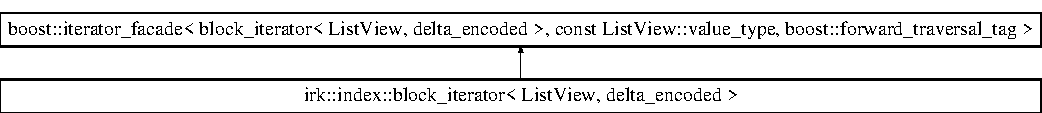
\includegraphics[height=1.523810cm]{classirk_1_1index_1_1block__iterator}
\end{center}
\end{figure}
\subsection*{Public Types}
\begin{DoxyCompactItemize}
\item 
using \mbox{\hyperlink{classirk_1_1index_1_1block__iterator_a75bc89b691db97f719af7284ee91afa0}{view\+\_\+type}} = List\+View
\item 
using \mbox{\hyperlink{classirk_1_1index_1_1block__iterator_a338ee8fee726492e9f8bbad4b4d75766}{self\+\_\+type}} = \mbox{\hyperlink{classirk_1_1index_1_1block__iterator}{block\+\_\+iterator}}$<$ \mbox{\hyperlink{classirk_1_1index_1_1block__iterator_a75bc89b691db97f719af7284ee91afa0}{view\+\_\+type}}, delta\+\_\+encoded $>$
\item 
using \mbox{\hyperlink{classirk_1_1index_1_1block__iterator_abb90b6c7a6100113770359e6eb9dd8cf}{difference\+\_\+type}} = int
\item 
using \mbox{\hyperlink{classirk_1_1index_1_1block__iterator_a4d6c5b58cedd871e8a8f235e425e8587}{value\+\_\+type}} = typename List\+View\+::value\+\_\+type
\end{DoxyCompactItemize}
\subsection*{Public Member Functions}
\begin{DoxyCompactItemize}
\item 
\mbox{\hyperlink{classirk_1_1index_1_1block__iterator_a00174f254405749a39d2009b2a6819bf}{block\+\_\+iterator}} (const \mbox{\hyperlink{classirk_1_1index_1_1block__iterator_a338ee8fee726492e9f8bbad4b4d75766}{self\+\_\+type}} \&)=default
\item 
\mbox{\hyperlink{classirk_1_1index_1_1block__iterator_ab166ce990eeb6efb45506acd57626042}{block\+\_\+iterator}} (\mbox{\hyperlink{classirk_1_1index_1_1block__iterator_a338ee8fee726492e9f8bbad4b4d75766}{self\+\_\+type}} \&\&) noexcept=default
\item 
\mbox{\hyperlink{classirk_1_1index_1_1block__iterator}{block\+\_\+iterator}} \& \mbox{\hyperlink{classirk_1_1index_1_1block__iterator_afc88fc6cd2cd2a148b821e5e89b6649a}{operator=}} (const \mbox{\hyperlink{classirk_1_1index_1_1block__iterator_a338ee8fee726492e9f8bbad4b4d75766}{self\+\_\+type}} \&)=delete
\item 
\mbox{\hyperlink{classirk_1_1index_1_1block__iterator}{block\+\_\+iterator}} \& \mbox{\hyperlink{classirk_1_1index_1_1block__iterator_a6696d285fe4899cb9aec7ac50fb09ad6}{operator=}} (\mbox{\hyperlink{classirk_1_1index_1_1block__iterator_a338ee8fee726492e9f8bbad4b4d75766}{self\+\_\+type}} \&\&) noexcept=delete
\item 
\mbox{\hyperlink{classirk_1_1index_1_1block__iterator_a6fd6578325dd4bcc585accac5782bf74}{$\sim$block\+\_\+iterator}} ()=default
\item 
\mbox{\hyperlink{classirk_1_1index_1_1block__iterator_ad68e07c02a8233cb098a23d57abf0e01}{block\+\_\+iterator}} (const \mbox{\hyperlink{classirk_1_1index_1_1block__iterator_a75bc89b691db97f719af7284ee91afa0}{view\+\_\+type}} \&view, \mbox{\hyperlink{classirk_1_1index_1_1block__iterator_abb90b6c7a6100113770359e6eb9dd8cf}{difference\+\_\+type}} \mbox{\hyperlink{classirk_1_1index_1_1block__iterator_afc0c06615fcd46d243bccd2a6a77ffeb}{block}}, \mbox{\hyperlink{classirk_1_1index_1_1block__iterator_abb90b6c7a6100113770359e6eb9dd8cf}{difference\+\_\+type}} \mbox{\hyperlink{classirk_1_1index_1_1block__iterator_a145b1a3e5f50d3eb0fc1135cda5f1253}{pos}}, int block\+\_\+size)
\item 
\mbox{\hyperlink{classirk_1_1index_1_1block__iterator_a338ee8fee726492e9f8bbad4b4d75766}{self\+\_\+type}} \& \mbox{\hyperlink{classirk_1_1index_1_1block__iterator_a7fd567ed2c5ece1ad02cf21957396c88}{moveto}} (\mbox{\hyperlink{classirk_1_1index_1_1block__iterator_a4d6c5b58cedd871e8a8f235e425e8587}{value\+\_\+type}} val)
\begin{DoxyCompactList}\small\item\em Move to the next position greater or equal {\ttfamily val}. \end{DoxyCompactList}\item 
\mbox{\hyperlink{classirk_1_1index_1_1block__iterator_a338ee8fee726492e9f8bbad4b4d75766}{self\+\_\+type}} \mbox{\hyperlink{classirk_1_1index_1_1block__iterator_aff7b154913783f7984e50c11efa10cb1}{nextgeq}} (\mbox{\hyperlink{classirk_1_1index_1_1block__iterator_a4d6c5b58cedd871e8a8f235e425e8587}{value\+\_\+type}} val)
\item 
{\footnotesize template$<$class Block\+Iterator $>$ }\\\mbox{\hyperlink{classirk_1_1index_1_1block__iterator_a338ee8fee726492e9f8bbad4b4d75766}{self\+\_\+type}} \& \mbox{\hyperlink{classirk_1_1index_1_1block__iterator_a901a557c429c737587e30b123bfc1641}{align}} (const Block\+Iterator \&other)
\begin{DoxyCompactList}\small\item\em Align this iterator to another. \end{DoxyCompactList}\item 
int \mbox{\hyperlink{classirk_1_1index_1_1block__iterator_afc0c06615fcd46d243bccd2a6a77ffeb}{block}} () const
\begin{DoxyCompactList}\small\item\em Returns the current block number. \end{DoxyCompactList}\item 
int \mbox{\hyperlink{classirk_1_1index_1_1block__iterator_a145b1a3e5f50d3eb0fc1135cda5f1253}{pos}} () const
\begin{DoxyCompactList}\small\item\em Returns the current position within the current block. \end{DoxyCompactList}\end{DoxyCompactItemize}
\subsection*{Friends}
\begin{DoxyCompactItemize}
\item 
class \mbox{\hyperlink{classirk_1_1index_1_1block__iterator_ac09f73e325921cc50ebcd96bed0f8096}{boost\+::iterator\+\_\+core\+\_\+access}}
\end{DoxyCompactItemize}


\subsection{Detailed Description}
\subsubsection*{template$<$class List\+View, bool delta\+\_\+encoded$>$\newline
class irk\+::index\+::block\+\_\+iterator$<$ List\+View, delta\+\_\+encoded $>$}

Block iterator. 


\begin{DoxyTemplParams}{Template Parameters}
{\em List\+View} & type of list (see \mbox{\hyperlink{classirk_1_1index_1_1block__document__list__view}{block\+\_\+document\+\_\+list\+\_\+view}} and \mbox{\hyperlink{classirk_1_1index_1_1block__payload__list__view}{block\+\_\+payload\+\_\+list\+\_\+view}}) \\
\hline
{\em delta\+\_\+encoded} & whether or not values are delta encoded; if so, an additional operation {\ttfamily \mbox{\hyperlink{classirk_1_1index_1_1block__iterator_aff7b154913783f7984e50c11efa10cb1}{nextgeq(value\+\_\+type)}}} is available to skip to the next greater or equal value\\
\hline
\end{DoxyTemplParams}
This iterator will decode and cache blocks that are accessed. The following operation will cause decoding of the entire block\+:
\begin{DoxyItemize}
\item dereferencing a value in a not yet decoded block;
\item {\ttfamily nextgeq} operation that reaches a not yet decoded block.
\end{DoxyItemize}

Any other operations will not decode or access any data. 

\subsection{Member Typedef Documentation}
\mbox{\Hypertarget{classirk_1_1index_1_1block__iterator_abb90b6c7a6100113770359e6eb9dd8cf}\label{classirk_1_1index_1_1block__iterator_abb90b6c7a6100113770359e6eb9dd8cf}} 
\index{irk\+::index\+::block\+\_\+iterator@{irk\+::index\+::block\+\_\+iterator}!difference\+\_\+type@{difference\+\_\+type}}
\index{difference\+\_\+type@{difference\+\_\+type}!irk\+::index\+::block\+\_\+iterator@{irk\+::index\+::block\+\_\+iterator}}
\subsubsection{\texorpdfstring{difference\+\_\+type}{difference\_type}}
{\footnotesize\ttfamily template$<$class List\+View , bool delta\+\_\+encoded$>$ \\
using \mbox{\hyperlink{classirk_1_1index_1_1block__iterator}{irk\+::index\+::block\+\_\+iterator}}$<$ List\+View, delta\+\_\+encoded $>$\+::\mbox{\hyperlink{classirk_1_1index_1_1block__iterator_abb90b6c7a6100113770359e6eb9dd8cf}{difference\+\_\+type}} =  int}

\mbox{\Hypertarget{classirk_1_1index_1_1block__iterator_a338ee8fee726492e9f8bbad4b4d75766}\label{classirk_1_1index_1_1block__iterator_a338ee8fee726492e9f8bbad4b4d75766}} 
\index{irk\+::index\+::block\+\_\+iterator@{irk\+::index\+::block\+\_\+iterator}!self\+\_\+type@{self\+\_\+type}}
\index{self\+\_\+type@{self\+\_\+type}!irk\+::index\+::block\+\_\+iterator@{irk\+::index\+::block\+\_\+iterator}}
\subsubsection{\texorpdfstring{self\+\_\+type}{self\_type}}
{\footnotesize\ttfamily template$<$class List\+View , bool delta\+\_\+encoded$>$ \\
using \mbox{\hyperlink{classirk_1_1index_1_1block__iterator}{irk\+::index\+::block\+\_\+iterator}}$<$ List\+View, delta\+\_\+encoded $>$\+::\mbox{\hyperlink{classirk_1_1index_1_1block__iterator_a338ee8fee726492e9f8bbad4b4d75766}{self\+\_\+type}} =  \mbox{\hyperlink{classirk_1_1index_1_1block__iterator}{block\+\_\+iterator}}$<$\mbox{\hyperlink{classirk_1_1index_1_1block__iterator_a75bc89b691db97f719af7284ee91afa0}{view\+\_\+type}}, delta\+\_\+encoded$>$}

\mbox{\Hypertarget{classirk_1_1index_1_1block__iterator_a4d6c5b58cedd871e8a8f235e425e8587}\label{classirk_1_1index_1_1block__iterator_a4d6c5b58cedd871e8a8f235e425e8587}} 
\index{irk\+::index\+::block\+\_\+iterator@{irk\+::index\+::block\+\_\+iterator}!value\+\_\+type@{value\+\_\+type}}
\index{value\+\_\+type@{value\+\_\+type}!irk\+::index\+::block\+\_\+iterator@{irk\+::index\+::block\+\_\+iterator}}
\subsubsection{\texorpdfstring{value\+\_\+type}{value\_type}}
{\footnotesize\ttfamily template$<$class List\+View , bool delta\+\_\+encoded$>$ \\
using \mbox{\hyperlink{classirk_1_1index_1_1block__iterator}{irk\+::index\+::block\+\_\+iterator}}$<$ List\+View, delta\+\_\+encoded $>$\+::\mbox{\hyperlink{classirk_1_1index_1_1block__iterator_a4d6c5b58cedd871e8a8f235e425e8587}{value\+\_\+type}} =  typename List\+View\+::value\+\_\+type}

\mbox{\Hypertarget{classirk_1_1index_1_1block__iterator_a75bc89b691db97f719af7284ee91afa0}\label{classirk_1_1index_1_1block__iterator_a75bc89b691db97f719af7284ee91afa0}} 
\index{irk\+::index\+::block\+\_\+iterator@{irk\+::index\+::block\+\_\+iterator}!view\+\_\+type@{view\+\_\+type}}
\index{view\+\_\+type@{view\+\_\+type}!irk\+::index\+::block\+\_\+iterator@{irk\+::index\+::block\+\_\+iterator}}
\subsubsection{\texorpdfstring{view\+\_\+type}{view\_type}}
{\footnotesize\ttfamily template$<$class List\+View , bool delta\+\_\+encoded$>$ \\
using \mbox{\hyperlink{classirk_1_1index_1_1block__iterator}{irk\+::index\+::block\+\_\+iterator}}$<$ List\+View, delta\+\_\+encoded $>$\+::\mbox{\hyperlink{classirk_1_1index_1_1block__iterator_a75bc89b691db97f719af7284ee91afa0}{view\+\_\+type}} =  List\+View}



\subsection{Constructor \& Destructor Documentation}
\mbox{\Hypertarget{classirk_1_1index_1_1block__iterator_a00174f254405749a39d2009b2a6819bf}\label{classirk_1_1index_1_1block__iterator_a00174f254405749a39d2009b2a6819bf}} 
\index{irk\+::index\+::block\+\_\+iterator@{irk\+::index\+::block\+\_\+iterator}!block\+\_\+iterator@{block\+\_\+iterator}}
\index{block\+\_\+iterator@{block\+\_\+iterator}!irk\+::index\+::block\+\_\+iterator@{irk\+::index\+::block\+\_\+iterator}}
\subsubsection{\texorpdfstring{block\+\_\+iterator()}{block\_iterator()}\hspace{0.1cm}{\footnotesize\ttfamily [1/3]}}
{\footnotesize\ttfamily template$<$class List\+View , bool delta\+\_\+encoded$>$ \\
\mbox{\hyperlink{classirk_1_1index_1_1block__iterator}{irk\+::index\+::block\+\_\+iterator}}$<$ List\+View, delta\+\_\+encoded $>$\+::\mbox{\hyperlink{classirk_1_1index_1_1block__iterator}{block\+\_\+iterator}} (\begin{DoxyParamCaption}\item[{const \mbox{\hyperlink{classirk_1_1index_1_1block__iterator_a338ee8fee726492e9f8bbad4b4d75766}{self\+\_\+type}} \&}]{ }\end{DoxyParamCaption})\hspace{0.3cm}{\ttfamily [default]}}

\mbox{\Hypertarget{classirk_1_1index_1_1block__iterator_ab166ce990eeb6efb45506acd57626042}\label{classirk_1_1index_1_1block__iterator_ab166ce990eeb6efb45506acd57626042}} 
\index{irk\+::index\+::block\+\_\+iterator@{irk\+::index\+::block\+\_\+iterator}!block\+\_\+iterator@{block\+\_\+iterator}}
\index{block\+\_\+iterator@{block\+\_\+iterator}!irk\+::index\+::block\+\_\+iterator@{irk\+::index\+::block\+\_\+iterator}}
\subsubsection{\texorpdfstring{block\+\_\+iterator()}{block\_iterator()}\hspace{0.1cm}{\footnotesize\ttfamily [2/3]}}
{\footnotesize\ttfamily template$<$class List\+View , bool delta\+\_\+encoded$>$ \\
\mbox{\hyperlink{classirk_1_1index_1_1block__iterator}{irk\+::index\+::block\+\_\+iterator}}$<$ List\+View, delta\+\_\+encoded $>$\+::\mbox{\hyperlink{classirk_1_1index_1_1block__iterator}{block\+\_\+iterator}} (\begin{DoxyParamCaption}\item[{\mbox{\hyperlink{classirk_1_1index_1_1block__iterator_a338ee8fee726492e9f8bbad4b4d75766}{self\+\_\+type}} \&\&}]{ }\end{DoxyParamCaption})\hspace{0.3cm}{\ttfamily [default]}, {\ttfamily [noexcept]}}

\mbox{\Hypertarget{classirk_1_1index_1_1block__iterator_a6fd6578325dd4bcc585accac5782bf74}\label{classirk_1_1index_1_1block__iterator_a6fd6578325dd4bcc585accac5782bf74}} 
\index{irk\+::index\+::block\+\_\+iterator@{irk\+::index\+::block\+\_\+iterator}!````~block\+\_\+iterator@{$\sim$block\+\_\+iterator}}
\index{````~block\+\_\+iterator@{$\sim$block\+\_\+iterator}!irk\+::index\+::block\+\_\+iterator@{irk\+::index\+::block\+\_\+iterator}}
\subsubsection{\texorpdfstring{$\sim$block\+\_\+iterator()}{~block\_iterator()}}
{\footnotesize\ttfamily template$<$class List\+View , bool delta\+\_\+encoded$>$ \\
\mbox{\hyperlink{classirk_1_1index_1_1block__iterator}{irk\+::index\+::block\+\_\+iterator}}$<$ List\+View, delta\+\_\+encoded $>$\+::$\sim$\mbox{\hyperlink{classirk_1_1index_1_1block__iterator}{block\+\_\+iterator}} (\begin{DoxyParamCaption}{ }\end{DoxyParamCaption})\hspace{0.3cm}{\ttfamily [default]}}

\mbox{\Hypertarget{classirk_1_1index_1_1block__iterator_ad68e07c02a8233cb098a23d57abf0e01}\label{classirk_1_1index_1_1block__iterator_ad68e07c02a8233cb098a23d57abf0e01}} 
\index{irk\+::index\+::block\+\_\+iterator@{irk\+::index\+::block\+\_\+iterator}!block\+\_\+iterator@{block\+\_\+iterator}}
\index{block\+\_\+iterator@{block\+\_\+iterator}!irk\+::index\+::block\+\_\+iterator@{irk\+::index\+::block\+\_\+iterator}}
\subsubsection{\texorpdfstring{block\+\_\+iterator()}{block\_iterator()}\hspace{0.1cm}{\footnotesize\ttfamily [3/3]}}
{\footnotesize\ttfamily template$<$class List\+View , bool delta\+\_\+encoded$>$ \\
\mbox{\hyperlink{classirk_1_1index_1_1block__iterator}{irk\+::index\+::block\+\_\+iterator}}$<$ List\+View, delta\+\_\+encoded $>$\+::\mbox{\hyperlink{classirk_1_1index_1_1block__iterator}{block\+\_\+iterator}} (\begin{DoxyParamCaption}\item[{const \mbox{\hyperlink{classirk_1_1index_1_1block__iterator_a75bc89b691db97f719af7284ee91afa0}{view\+\_\+type}} \&}]{view,  }\item[{\mbox{\hyperlink{classirk_1_1index_1_1block__iterator_abb90b6c7a6100113770359e6eb9dd8cf}{difference\+\_\+type}}}]{block,  }\item[{\mbox{\hyperlink{classirk_1_1index_1_1block__iterator_abb90b6c7a6100113770359e6eb9dd8cf}{difference\+\_\+type}}}]{pos,  }\item[{int}]{block\+\_\+size }\end{DoxyParamCaption})\hspace{0.3cm}{\ttfamily [inline]}}

The iterator is strictly connected to a list view and it stores a const reference to it internally. However, for performance reasons, when comparing iterators, it is not checked whether they belong to the same list\+: this check must be performed by the user if required. 

\subsection{Member Function Documentation}
\mbox{\Hypertarget{classirk_1_1index_1_1block__iterator_a901a557c429c737587e30b123bfc1641}\label{classirk_1_1index_1_1block__iterator_a901a557c429c737587e30b123bfc1641}} 
\index{irk\+::index\+::block\+\_\+iterator@{irk\+::index\+::block\+\_\+iterator}!align@{align}}
\index{align@{align}!irk\+::index\+::block\+\_\+iterator@{irk\+::index\+::block\+\_\+iterator}}
\subsubsection{\texorpdfstring{align()}{align()}}
{\footnotesize\ttfamily template$<$class List\+View , bool delta\+\_\+encoded$>$ \\
template$<$class Block\+Iterator $>$ \\
\mbox{\hyperlink{classirk_1_1index_1_1block__iterator_a338ee8fee726492e9f8bbad4b4d75766}{self\+\_\+type}}\& \mbox{\hyperlink{classirk_1_1index_1_1block__iterator}{irk\+::index\+::block\+\_\+iterator}}$<$ List\+View, delta\+\_\+encoded $>$\+::align (\begin{DoxyParamCaption}\item[{const Block\+Iterator \&}]{other }\end{DoxyParamCaption})\hspace{0.3cm}{\ttfamily [inline]}}



Align this iterator to another. 

Sets the position of this iterator to the position of {\ttfamily other}. Both lists should have the same length and block size, but this is not checked at runtime! \mbox{\Hypertarget{classirk_1_1index_1_1block__iterator_afc0c06615fcd46d243bccd2a6a77ffeb}\label{classirk_1_1index_1_1block__iterator_afc0c06615fcd46d243bccd2a6a77ffeb}} 
\index{irk\+::index\+::block\+\_\+iterator@{irk\+::index\+::block\+\_\+iterator}!block@{block}}
\index{block@{block}!irk\+::index\+::block\+\_\+iterator@{irk\+::index\+::block\+\_\+iterator}}
\subsubsection{\texorpdfstring{block()}{block()}}
{\footnotesize\ttfamily template$<$class List\+View , bool delta\+\_\+encoded$>$ \\
int \mbox{\hyperlink{classirk_1_1index_1_1block__iterator}{irk\+::index\+::block\+\_\+iterator}}$<$ List\+View, delta\+\_\+encoded $>$\+::block (\begin{DoxyParamCaption}{ }\end{DoxyParamCaption}) const\hspace{0.3cm}{\ttfamily [inline]}}



Returns the current block number. 

\mbox{\Hypertarget{classirk_1_1index_1_1block__iterator_a7fd567ed2c5ece1ad02cf21957396c88}\label{classirk_1_1index_1_1block__iterator_a7fd567ed2c5ece1ad02cf21957396c88}} 
\index{irk\+::index\+::block\+\_\+iterator@{irk\+::index\+::block\+\_\+iterator}!moveto@{moveto}}
\index{moveto@{moveto}!irk\+::index\+::block\+\_\+iterator@{irk\+::index\+::block\+\_\+iterator}}
\subsubsection{\texorpdfstring{moveto()}{moveto()}}
{\footnotesize\ttfamily template$<$class List\+View , bool delta\+\_\+encoded$>$ \\
\mbox{\hyperlink{classirk_1_1index_1_1block__iterator_a338ee8fee726492e9f8bbad4b4d75766}{self\+\_\+type}}\& \mbox{\hyperlink{classirk_1_1index_1_1block__iterator}{irk\+::index\+::block\+\_\+iterator}}$<$ List\+View, delta\+\_\+encoded $>$\+::moveto (\begin{DoxyParamCaption}\item[{\mbox{\hyperlink{classirk_1_1index_1_1block__iterator_a4d6c5b58cedd871e8a8f235e425e8587}{value\+\_\+type}}}]{val }\end{DoxyParamCaption})\hspace{0.3cm}{\ttfamily [inline]}}



Move to the next position greater or equal {\ttfamily val}. 


\begin{DoxyParams}{Parameters}
{\em val} & the value to look up; if does not exist, point to the next greater value; if neither exist, point to {\ttfamily end()} \\
\hline
\end{DoxyParams}
\begin{DoxyReturn}{Returns}
{\ttfamily $\ast$this} after finding position
\end{DoxyReturn}
The lookup starts from the current position. If the next value {\ttfamily $>$= val} exists in a still encoded block, it will be decoded and cached. If all values from the current position forward are {\ttfamily $<$ val}, then the resulting iterator will point after the last element (equivalent to calling {\ttfamily end()} on the list view). \mbox{\Hypertarget{classirk_1_1index_1_1block__iterator_aff7b154913783f7984e50c11efa10cb1}\label{classirk_1_1index_1_1block__iterator_aff7b154913783f7984e50c11efa10cb1}} 
\index{irk\+::index\+::block\+\_\+iterator@{irk\+::index\+::block\+\_\+iterator}!nextgeq@{nextgeq}}
\index{nextgeq@{nextgeq}!irk\+::index\+::block\+\_\+iterator@{irk\+::index\+::block\+\_\+iterator}}
\subsubsection{\texorpdfstring{nextgeq()}{nextgeq()}}
{\footnotesize\ttfamily template$<$class List\+View , bool delta\+\_\+encoded$>$ \\
\mbox{\hyperlink{classirk_1_1index_1_1block__iterator_a338ee8fee726492e9f8bbad4b4d75766}{self\+\_\+type}} \mbox{\hyperlink{classirk_1_1index_1_1block__iterator}{irk\+::index\+::block\+\_\+iterator}}$<$ List\+View, delta\+\_\+encoded $>$\+::nextgeq (\begin{DoxyParamCaption}\item[{\mbox{\hyperlink{classirk_1_1index_1_1block__iterator_a4d6c5b58cedd871e8a8f235e425e8587}{value\+\_\+type}}}]{val }\end{DoxyParamCaption})\hspace{0.3cm}{\ttfamily [inline]}}

\mbox{\Hypertarget{classirk_1_1index_1_1block__iterator_afc88fc6cd2cd2a148b821e5e89b6649a}\label{classirk_1_1index_1_1block__iterator_afc88fc6cd2cd2a148b821e5e89b6649a}} 
\index{irk\+::index\+::block\+\_\+iterator@{irk\+::index\+::block\+\_\+iterator}!operator=@{operator=}}
\index{operator=@{operator=}!irk\+::index\+::block\+\_\+iterator@{irk\+::index\+::block\+\_\+iterator}}
\subsubsection{\texorpdfstring{operator=()}{operator=()}\hspace{0.1cm}{\footnotesize\ttfamily [1/2]}}
{\footnotesize\ttfamily template$<$class List\+View , bool delta\+\_\+encoded$>$ \\
\mbox{\hyperlink{classirk_1_1index_1_1block__iterator}{block\+\_\+iterator}}\& \mbox{\hyperlink{classirk_1_1index_1_1block__iterator}{irk\+::index\+::block\+\_\+iterator}}$<$ List\+View, delta\+\_\+encoded $>$\+::operator= (\begin{DoxyParamCaption}\item[{const \mbox{\hyperlink{classirk_1_1index_1_1block__iterator_a338ee8fee726492e9f8bbad4b4d75766}{self\+\_\+type}} \&}]{ }\end{DoxyParamCaption})\hspace{0.3cm}{\ttfamily [delete]}}

\mbox{\Hypertarget{classirk_1_1index_1_1block__iterator_a6696d285fe4899cb9aec7ac50fb09ad6}\label{classirk_1_1index_1_1block__iterator_a6696d285fe4899cb9aec7ac50fb09ad6}} 
\index{irk\+::index\+::block\+\_\+iterator@{irk\+::index\+::block\+\_\+iterator}!operator=@{operator=}}
\index{operator=@{operator=}!irk\+::index\+::block\+\_\+iterator@{irk\+::index\+::block\+\_\+iterator}}
\subsubsection{\texorpdfstring{operator=()}{operator=()}\hspace{0.1cm}{\footnotesize\ttfamily [2/2]}}
{\footnotesize\ttfamily template$<$class List\+View , bool delta\+\_\+encoded$>$ \\
\mbox{\hyperlink{classirk_1_1index_1_1block__iterator}{block\+\_\+iterator}}\& \mbox{\hyperlink{classirk_1_1index_1_1block__iterator}{irk\+::index\+::block\+\_\+iterator}}$<$ List\+View, delta\+\_\+encoded $>$\+::operator= (\begin{DoxyParamCaption}\item[{\mbox{\hyperlink{classirk_1_1index_1_1block__iterator_a338ee8fee726492e9f8bbad4b4d75766}{self\+\_\+type}} \&\&}]{ }\end{DoxyParamCaption})\hspace{0.3cm}{\ttfamily [delete]}, {\ttfamily [noexcept]}}

\mbox{\Hypertarget{classirk_1_1index_1_1block__iterator_a145b1a3e5f50d3eb0fc1135cda5f1253}\label{classirk_1_1index_1_1block__iterator_a145b1a3e5f50d3eb0fc1135cda5f1253}} 
\index{irk\+::index\+::block\+\_\+iterator@{irk\+::index\+::block\+\_\+iterator}!pos@{pos}}
\index{pos@{pos}!irk\+::index\+::block\+\_\+iterator@{irk\+::index\+::block\+\_\+iterator}}
\subsubsection{\texorpdfstring{pos()}{pos()}}
{\footnotesize\ttfamily template$<$class List\+View , bool delta\+\_\+encoded$>$ \\
int \mbox{\hyperlink{classirk_1_1index_1_1block__iterator}{irk\+::index\+::block\+\_\+iterator}}$<$ List\+View, delta\+\_\+encoded $>$\+::pos (\begin{DoxyParamCaption}{ }\end{DoxyParamCaption}) const\hspace{0.3cm}{\ttfamily [inline]}}



Returns the current position within the current block. 



\subsection{Friends And Related Function Documentation}
\mbox{\Hypertarget{classirk_1_1index_1_1block__iterator_ac09f73e325921cc50ebcd96bed0f8096}\label{classirk_1_1index_1_1block__iterator_ac09f73e325921cc50ebcd96bed0f8096}} 
\index{irk\+::index\+::block\+\_\+iterator@{irk\+::index\+::block\+\_\+iterator}!boost\+::iterator\+\_\+core\+\_\+access@{boost\+::iterator\+\_\+core\+\_\+access}}
\index{boost\+::iterator\+\_\+core\+\_\+access@{boost\+::iterator\+\_\+core\+\_\+access}!irk\+::index\+::block\+\_\+iterator@{irk\+::index\+::block\+\_\+iterator}}
\subsubsection{\texorpdfstring{boost\+::iterator\+\_\+core\+\_\+access}{boost::iterator\_core\_access}}
{\footnotesize\ttfamily template$<$class List\+View , bool delta\+\_\+encoded$>$ \\
friend class boost\+::iterator\+\_\+core\+\_\+access\hspace{0.3cm}{\ttfamily [friend]}}



The documentation for this class was generated from the following file\+:\begin{DoxyCompactItemize}
\item 
include/irkit/index/\mbox{\hyperlink{block__inverted__list_8hpp}{block\+\_\+inverted\+\_\+list.\+hpp}}\end{DoxyCompactItemize}

\hypertarget{classirk_1_1index_1_1block__list__builder}{}\section{irk\+:\+:index\+:\+:block\+\_\+list\+\_\+builder$<$ Value, Codec, delta\+\_\+encoded $>$ Class Template Reference}
\label{classirk_1_1index_1_1block__list__builder}\index{irk\+::index\+::block\+\_\+list\+\_\+builder$<$ Value, Codec, delta\+\_\+encoded $>$@{irk\+::index\+::block\+\_\+list\+\_\+builder$<$ Value, Codec, delta\+\_\+encoded $>$}}


{\ttfamily \#include $<$block\+\_\+inverted\+\_\+list.\+hpp$>$}

\subsection*{Public Types}
\begin{DoxyCompactItemize}
\item 
using \mbox{\hyperlink{classirk_1_1index_1_1block__list__builder_a5f67d973ddc3719baf9b62e19c6ab875}{codec\+\_\+type}} = Codec
\item 
using \mbox{\hyperlink{classirk_1_1index_1_1block__list__builder_aee4746d79079e00283a5f7a3ad071b5e}{value\+\_\+type}} = Value
\item 
using \mbox{\hyperlink{classirk_1_1index_1_1block__list__builder_a860cd8cc2694c917a48d1de1c221d00f}{encoding\+\_\+device}} = boost\+::iostreams\+::back\+\_\+insert\+\_\+device$<$ std\+::vector$<$ char $>$ $>$
\end{DoxyCompactItemize}
\subsection*{Public Member Functions}
\begin{DoxyCompactItemize}
\item 
\mbox{\hyperlink{classirk_1_1index_1_1block__list__builder_a7d34ddbad0ae90c5623689f194e21571}{block\+\_\+list\+\_\+builder}} (int block\+\_\+size)
\item 
void \mbox{\hyperlink{classirk_1_1index_1_1block__list__builder_a689ecb66563dd8ccdfd26d103da377a3}{add}} (\mbox{\hyperlink{classirk_1_1index_1_1block__list__builder_aee4746d79079e00283a5f7a3ad071b5e}{value\+\_\+type}} id)
\item 
std\+::streamsize \mbox{\hyperlink{classirk_1_1index_1_1block__list__builder_a003cb5e11a447ddf8ae03da4ba47a036}{write}} (std\+::ostream \&out) const
\end{DoxyCompactItemize}


\subsection{Member Typedef Documentation}
\mbox{\Hypertarget{classirk_1_1index_1_1block__list__builder_a5f67d973ddc3719baf9b62e19c6ab875}\label{classirk_1_1index_1_1block__list__builder_a5f67d973ddc3719baf9b62e19c6ab875}} 
\index{irk\+::index\+::block\+\_\+list\+\_\+builder@{irk\+::index\+::block\+\_\+list\+\_\+builder}!codec\+\_\+type@{codec\+\_\+type}}
\index{codec\+\_\+type@{codec\+\_\+type}!irk\+::index\+::block\+\_\+list\+\_\+builder@{irk\+::index\+::block\+\_\+list\+\_\+builder}}
\subsubsection{\texorpdfstring{codec\+\_\+type}{codec\_type}}
{\footnotesize\ttfamily template$<$class Value, class Codec, bool delta\+\_\+encoded = false$>$ \\
using \mbox{\hyperlink{classirk_1_1index_1_1block__list__builder}{irk\+::index\+::block\+\_\+list\+\_\+builder}}$<$ Value, Codec, delta\+\_\+encoded $>$\+::\mbox{\hyperlink{classirk_1_1index_1_1block__list__builder_a5f67d973ddc3719baf9b62e19c6ab875}{codec\+\_\+type}} =  Codec}

\mbox{\Hypertarget{classirk_1_1index_1_1block__list__builder_a860cd8cc2694c917a48d1de1c221d00f}\label{classirk_1_1index_1_1block__list__builder_a860cd8cc2694c917a48d1de1c221d00f}} 
\index{irk\+::index\+::block\+\_\+list\+\_\+builder@{irk\+::index\+::block\+\_\+list\+\_\+builder}!encoding\+\_\+device@{encoding\+\_\+device}}
\index{encoding\+\_\+device@{encoding\+\_\+device}!irk\+::index\+::block\+\_\+list\+\_\+builder@{irk\+::index\+::block\+\_\+list\+\_\+builder}}
\subsubsection{\texorpdfstring{encoding\+\_\+device}{encoding\_device}}
{\footnotesize\ttfamily template$<$class Value, class Codec, bool delta\+\_\+encoded = false$>$ \\
using \mbox{\hyperlink{classirk_1_1index_1_1block__list__builder}{irk\+::index\+::block\+\_\+list\+\_\+builder}}$<$ Value, Codec, delta\+\_\+encoded $>$\+::\mbox{\hyperlink{classirk_1_1index_1_1block__list__builder_a860cd8cc2694c917a48d1de1c221d00f}{encoding\+\_\+device}} =  boost\+::iostreams\+::back\+\_\+insert\+\_\+device$<$std\+::vector$<$char$>$ $>$}

\mbox{\Hypertarget{classirk_1_1index_1_1block__list__builder_aee4746d79079e00283a5f7a3ad071b5e}\label{classirk_1_1index_1_1block__list__builder_aee4746d79079e00283a5f7a3ad071b5e}} 
\index{irk\+::index\+::block\+\_\+list\+\_\+builder@{irk\+::index\+::block\+\_\+list\+\_\+builder}!value\+\_\+type@{value\+\_\+type}}
\index{value\+\_\+type@{value\+\_\+type}!irk\+::index\+::block\+\_\+list\+\_\+builder@{irk\+::index\+::block\+\_\+list\+\_\+builder}}
\subsubsection{\texorpdfstring{value\+\_\+type}{value\_type}}
{\footnotesize\ttfamily template$<$class Value, class Codec, bool delta\+\_\+encoded = false$>$ \\
using \mbox{\hyperlink{classirk_1_1index_1_1block__list__builder}{irk\+::index\+::block\+\_\+list\+\_\+builder}}$<$ Value, Codec, delta\+\_\+encoded $>$\+::\mbox{\hyperlink{classirk_1_1index_1_1block__list__builder_aee4746d79079e00283a5f7a3ad071b5e}{value\+\_\+type}} =  Value}



\subsection{Constructor \& Destructor Documentation}
\mbox{\Hypertarget{classirk_1_1index_1_1block__list__builder_a7d34ddbad0ae90c5623689f194e21571}\label{classirk_1_1index_1_1block__list__builder_a7d34ddbad0ae90c5623689f194e21571}} 
\index{irk\+::index\+::block\+\_\+list\+\_\+builder@{irk\+::index\+::block\+\_\+list\+\_\+builder}!block\+\_\+list\+\_\+builder@{block\+\_\+list\+\_\+builder}}
\index{block\+\_\+list\+\_\+builder@{block\+\_\+list\+\_\+builder}!irk\+::index\+::block\+\_\+list\+\_\+builder@{irk\+::index\+::block\+\_\+list\+\_\+builder}}
\subsubsection{\texorpdfstring{block\+\_\+list\+\_\+builder()}{block\_list\_builder()}}
{\footnotesize\ttfamily template$<$class Value, class Codec, bool delta\+\_\+encoded = false$>$ \\
\mbox{\hyperlink{classirk_1_1index_1_1block__list__builder}{irk\+::index\+::block\+\_\+list\+\_\+builder}}$<$ Value, Codec, delta\+\_\+encoded $>$\+::\mbox{\hyperlink{classirk_1_1index_1_1block__list__builder}{block\+\_\+list\+\_\+builder}} (\begin{DoxyParamCaption}\item[{int}]{block\+\_\+size }\end{DoxyParamCaption})\hspace{0.3cm}{\ttfamily [inline]}, {\ttfamily [explicit]}}



\subsection{Member Function Documentation}
\mbox{\Hypertarget{classirk_1_1index_1_1block__list__builder_a689ecb66563dd8ccdfd26d103da377a3}\label{classirk_1_1index_1_1block__list__builder_a689ecb66563dd8ccdfd26d103da377a3}} 
\index{irk\+::index\+::block\+\_\+list\+\_\+builder@{irk\+::index\+::block\+\_\+list\+\_\+builder}!add@{add}}
\index{add@{add}!irk\+::index\+::block\+\_\+list\+\_\+builder@{irk\+::index\+::block\+\_\+list\+\_\+builder}}
\subsubsection{\texorpdfstring{add()}{add()}}
{\footnotesize\ttfamily template$<$class Value, class Codec, bool delta\+\_\+encoded = false$>$ \\
void \mbox{\hyperlink{classirk_1_1index_1_1block__list__builder}{irk\+::index\+::block\+\_\+list\+\_\+builder}}$<$ Value, Codec, delta\+\_\+encoded $>$\+::add (\begin{DoxyParamCaption}\item[{\mbox{\hyperlink{classirk_1_1index_1_1block__list__builder_aee4746d79079e00283a5f7a3ad071b5e}{value\+\_\+type}}}]{id }\end{DoxyParamCaption})\hspace{0.3cm}{\ttfamily [inline]}}

\mbox{\Hypertarget{classirk_1_1index_1_1block__list__builder_a003cb5e11a447ddf8ae03da4ba47a036}\label{classirk_1_1index_1_1block__list__builder_a003cb5e11a447ddf8ae03da4ba47a036}} 
\index{irk\+::index\+::block\+\_\+list\+\_\+builder@{irk\+::index\+::block\+\_\+list\+\_\+builder}!write@{write}}
\index{write@{write}!irk\+::index\+::block\+\_\+list\+\_\+builder@{irk\+::index\+::block\+\_\+list\+\_\+builder}}
\subsubsection{\texorpdfstring{write()}{write()}}
{\footnotesize\ttfamily template$<$class Value, class Codec, bool delta\+\_\+encoded = false$>$ \\
std\+::streamsize \mbox{\hyperlink{classirk_1_1index_1_1block__list__builder}{irk\+::index\+::block\+\_\+list\+\_\+builder}}$<$ Value, Codec, delta\+\_\+encoded $>$\+::write (\begin{DoxyParamCaption}\item[{std\+::ostream \&}]{out }\end{DoxyParamCaption}) const\hspace{0.3cm}{\ttfamily [inline]}}



The documentation for this class was generated from the following file\+:\begin{DoxyCompactItemize}
\item 
include/irkit/index/\mbox{\hyperlink{block__inverted__list_8hpp}{block\+\_\+inverted\+\_\+list.\+hpp}}\end{DoxyCompactItemize}

\hypertarget{classirk_1_1index_1_1block__payload__list__view}{}\section{irk\+:\+:index\+:\+:block\+\_\+payload\+\_\+list\+\_\+view$<$ Payload $>$ Class Template Reference}
\label{classirk_1_1index_1_1block__payload__list__view}\index{irk\+::index\+::block\+\_\+payload\+\_\+list\+\_\+view$<$ Payload $>$@{irk\+::index\+::block\+\_\+payload\+\_\+list\+\_\+view$<$ Payload $>$}}


A view of a block payload list.  




{\ttfamily \#include $<$block\+\_\+inverted\+\_\+list.\+hpp$>$}

\subsection*{Public Types}
\begin{DoxyCompactItemize}
\item 
using \mbox{\hyperlink{classirk_1_1index_1_1block__payload__list__view_aa7545a3c9095406fb90e0dca7b146b60}{size\+\_\+type}} = int
\item 
using \mbox{\hyperlink{classirk_1_1index_1_1block__payload__list__view_a739d436330ba54972ef70a5cd3f57ef3}{value\+\_\+type}} = Payload
\item 
using \mbox{\hyperlink{classirk_1_1index_1_1block__payload__list__view_a29e1995bbc64a8512bacf6c110f24f9e}{self\+\_\+type}} = \mbox{\hyperlink{classirk_1_1index_1_1block__payload__list__view}{block\+\_\+payload\+\_\+list\+\_\+view}}$<$ \mbox{\hyperlink{classirk_1_1index_1_1block__payload__list__view_a739d436330ba54972ef70a5cd3f57ef3}{value\+\_\+type}} $>$
\item 
using \mbox{\hyperlink{classirk_1_1index_1_1block__payload__list__view_a3cbb6ab331804c87e830be1380a3c2b2}{iterator}} = \mbox{\hyperlink{classirk_1_1index_1_1block__iterator}{block\+\_\+iterator}}$<$ \mbox{\hyperlink{classirk_1_1index_1_1block__payload__list__view_a29e1995bbc64a8512bacf6c110f24f9e}{self\+\_\+type}}, false $>$
\end{DoxyCompactItemize}
\subsection*{Public Member Functions}
\begin{DoxyCompactItemize}
\item 
\mbox{\hyperlink{classirk_1_1index_1_1block__payload__list__view_a1e4549a450e5fa10e0be7e7f49258d32}{block\+\_\+payload\+\_\+list\+\_\+view}} ()
\item 
\mbox{\hyperlink{classirk_1_1index_1_1block__payload__list__view_ac4e12722967b36c60ef7eff0209f9ba5}{block\+\_\+payload\+\_\+list\+\_\+view}} (\mbox{\hyperlink{namespaceirk_a831a3a869cf19601dbfb5c41765a2e87}{any\+\_\+codec}}$<$ \mbox{\hyperlink{classirk_1_1index_1_1block__payload__list__view_a739d436330ba54972ef70a5cd3f57ef3}{value\+\_\+type}} $>$ payload\+\_\+codec, \mbox{\hyperlink{classirk_1_1memory__view}{irk\+::memory\+\_\+view}} mem, long length, int offset=0)
\begin{DoxyCompactList}\small\item\em Constructs the view. \end{DoxyCompactList}\item 
\mbox{\hyperlink{classirk_1_1index_1_1block__payload__list__view_a3cbb6ab331804c87e830be1380a3c2b2}{iterator}} \mbox{\hyperlink{classirk_1_1index_1_1block__payload__list__view_a32284b7ff4f4c6530a43b9148418348f}{begin}} () const
\item 
\mbox{\hyperlink{classirk_1_1index_1_1block__payload__list__view_a3cbb6ab331804c87e830be1380a3c2b2}{iterator}} \mbox{\hyperlink{classirk_1_1index_1_1block__payload__list__view_a0daeb1ce7d6b877d6345067956dd8c9e}{end}} () const
\item 
long \mbox{\hyperlink{classirk_1_1index_1_1block__payload__list__view_a39a195ac21c15a74c42c89f54dfbcbac}{size}} () const
\end{DoxyCompactItemize}
\subsection*{Friends}
\begin{DoxyCompactItemize}
\item 
class \mbox{\hyperlink{classirk_1_1index_1_1block__payload__list__view_a88a9a271d334c6a1ee36182f15227581}{block\+\_\+iterator$<$ self\+\_\+type, false $>$}}
\end{DoxyCompactItemize}


\subsection{Detailed Description}
\subsubsection*{template$<$class Payload$>$\newline
class irk\+::index\+::block\+\_\+payload\+\_\+list\+\_\+view$<$ Payload $>$}

A view of a block payload list. 


\begin{DoxyTemplParams}{Template Parameters}
{\em Payload} & type of the payload, must be primitive type \\
\hline
\end{DoxyTemplParams}


\subsection{Member Typedef Documentation}
\mbox{\Hypertarget{classirk_1_1index_1_1block__payload__list__view_a3cbb6ab331804c87e830be1380a3c2b2}\label{classirk_1_1index_1_1block__payload__list__view_a3cbb6ab331804c87e830be1380a3c2b2}} 
\index{irk\+::index\+::block\+\_\+payload\+\_\+list\+\_\+view@{irk\+::index\+::block\+\_\+payload\+\_\+list\+\_\+view}!iterator@{iterator}}
\index{iterator@{iterator}!irk\+::index\+::block\+\_\+payload\+\_\+list\+\_\+view@{irk\+::index\+::block\+\_\+payload\+\_\+list\+\_\+view}}
\subsubsection{\texorpdfstring{iterator}{iterator}}
{\footnotesize\ttfamily template$<$class Payload$>$ \\
using \mbox{\hyperlink{classirk_1_1index_1_1block__payload__list__view}{irk\+::index\+::block\+\_\+payload\+\_\+list\+\_\+view}}$<$ Payload $>$\+::\mbox{\hyperlink{classirk_1_1index_1_1block__payload__list__view_a3cbb6ab331804c87e830be1380a3c2b2}{iterator}} =  \mbox{\hyperlink{classirk_1_1index_1_1block__iterator}{block\+\_\+iterator}}$<$\mbox{\hyperlink{classirk_1_1index_1_1block__payload__list__view_a29e1995bbc64a8512bacf6c110f24f9e}{self\+\_\+type}}, false$>$}

\mbox{\Hypertarget{classirk_1_1index_1_1block__payload__list__view_a29e1995bbc64a8512bacf6c110f24f9e}\label{classirk_1_1index_1_1block__payload__list__view_a29e1995bbc64a8512bacf6c110f24f9e}} 
\index{irk\+::index\+::block\+\_\+payload\+\_\+list\+\_\+view@{irk\+::index\+::block\+\_\+payload\+\_\+list\+\_\+view}!self\+\_\+type@{self\+\_\+type}}
\index{self\+\_\+type@{self\+\_\+type}!irk\+::index\+::block\+\_\+payload\+\_\+list\+\_\+view@{irk\+::index\+::block\+\_\+payload\+\_\+list\+\_\+view}}
\subsubsection{\texorpdfstring{self\+\_\+type}{self\_type}}
{\footnotesize\ttfamily template$<$class Payload$>$ \\
using \mbox{\hyperlink{classirk_1_1index_1_1block__payload__list__view}{irk\+::index\+::block\+\_\+payload\+\_\+list\+\_\+view}}$<$ Payload $>$\+::\mbox{\hyperlink{classirk_1_1index_1_1block__payload__list__view_a29e1995bbc64a8512bacf6c110f24f9e}{self\+\_\+type}} =  \mbox{\hyperlink{classirk_1_1index_1_1block__payload__list__view}{block\+\_\+payload\+\_\+list\+\_\+view}}$<$\mbox{\hyperlink{classirk_1_1index_1_1block__payload__list__view_a739d436330ba54972ef70a5cd3f57ef3}{value\+\_\+type}}$>$}

\mbox{\Hypertarget{classirk_1_1index_1_1block__payload__list__view_aa7545a3c9095406fb90e0dca7b146b60}\label{classirk_1_1index_1_1block__payload__list__view_aa7545a3c9095406fb90e0dca7b146b60}} 
\index{irk\+::index\+::block\+\_\+payload\+\_\+list\+\_\+view@{irk\+::index\+::block\+\_\+payload\+\_\+list\+\_\+view}!size\+\_\+type@{size\+\_\+type}}
\index{size\+\_\+type@{size\+\_\+type}!irk\+::index\+::block\+\_\+payload\+\_\+list\+\_\+view@{irk\+::index\+::block\+\_\+payload\+\_\+list\+\_\+view}}
\subsubsection{\texorpdfstring{size\+\_\+type}{size\_type}}
{\footnotesize\ttfamily template$<$class Payload$>$ \\
using \mbox{\hyperlink{classirk_1_1index_1_1block__payload__list__view}{irk\+::index\+::block\+\_\+payload\+\_\+list\+\_\+view}}$<$ Payload $>$\+::\mbox{\hyperlink{classirk_1_1index_1_1block__payload__list__view_aa7545a3c9095406fb90e0dca7b146b60}{size\+\_\+type}} =  int}

\mbox{\Hypertarget{classirk_1_1index_1_1block__payload__list__view_a739d436330ba54972ef70a5cd3f57ef3}\label{classirk_1_1index_1_1block__payload__list__view_a739d436330ba54972ef70a5cd3f57ef3}} 
\index{irk\+::index\+::block\+\_\+payload\+\_\+list\+\_\+view@{irk\+::index\+::block\+\_\+payload\+\_\+list\+\_\+view}!value\+\_\+type@{value\+\_\+type}}
\index{value\+\_\+type@{value\+\_\+type}!irk\+::index\+::block\+\_\+payload\+\_\+list\+\_\+view@{irk\+::index\+::block\+\_\+payload\+\_\+list\+\_\+view}}
\subsubsection{\texorpdfstring{value\+\_\+type}{value\_type}}
{\footnotesize\ttfamily template$<$class Payload$>$ \\
using \mbox{\hyperlink{classirk_1_1index_1_1block__payload__list__view}{irk\+::index\+::block\+\_\+payload\+\_\+list\+\_\+view}}$<$ Payload $>$\+::\mbox{\hyperlink{classirk_1_1index_1_1block__payload__list__view_a739d436330ba54972ef70a5cd3f57ef3}{value\+\_\+type}} =  Payload}



\subsection{Constructor \& Destructor Documentation}
\mbox{\Hypertarget{classirk_1_1index_1_1block__payload__list__view_a1e4549a450e5fa10e0be7e7f49258d32}\label{classirk_1_1index_1_1block__payload__list__view_a1e4549a450e5fa10e0be7e7f49258d32}} 
\index{irk\+::index\+::block\+\_\+payload\+\_\+list\+\_\+view@{irk\+::index\+::block\+\_\+payload\+\_\+list\+\_\+view}!block\+\_\+payload\+\_\+list\+\_\+view@{block\+\_\+payload\+\_\+list\+\_\+view}}
\index{block\+\_\+payload\+\_\+list\+\_\+view@{block\+\_\+payload\+\_\+list\+\_\+view}!irk\+::index\+::block\+\_\+payload\+\_\+list\+\_\+view@{irk\+::index\+::block\+\_\+payload\+\_\+list\+\_\+view}}
\subsubsection{\texorpdfstring{block\+\_\+payload\+\_\+list\+\_\+view()}{block\_payload\_list\_view()}\hspace{0.1cm}{\footnotesize\ttfamily [1/2]}}
{\footnotesize\ttfamily template$<$class Payload$>$ \\
\mbox{\hyperlink{classirk_1_1index_1_1block__payload__list__view}{irk\+::index\+::block\+\_\+payload\+\_\+list\+\_\+view}}$<$ Payload $>$\+::\mbox{\hyperlink{classirk_1_1index_1_1block__payload__list__view}{block\+\_\+payload\+\_\+list\+\_\+view}} (\begin{DoxyParamCaption}{ }\end{DoxyParamCaption})\hspace{0.3cm}{\ttfamily [inline]}}

\mbox{\Hypertarget{classirk_1_1index_1_1block__payload__list__view_ac4e12722967b36c60ef7eff0209f9ba5}\label{classirk_1_1index_1_1block__payload__list__view_ac4e12722967b36c60ef7eff0209f9ba5}} 
\index{irk\+::index\+::block\+\_\+payload\+\_\+list\+\_\+view@{irk\+::index\+::block\+\_\+payload\+\_\+list\+\_\+view}!block\+\_\+payload\+\_\+list\+\_\+view@{block\+\_\+payload\+\_\+list\+\_\+view}}
\index{block\+\_\+payload\+\_\+list\+\_\+view@{block\+\_\+payload\+\_\+list\+\_\+view}!irk\+::index\+::block\+\_\+payload\+\_\+list\+\_\+view@{irk\+::index\+::block\+\_\+payload\+\_\+list\+\_\+view}}
\subsubsection{\texorpdfstring{block\+\_\+payload\+\_\+list\+\_\+view()}{block\_payload\_list\_view()}\hspace{0.1cm}{\footnotesize\ttfamily [2/2]}}
{\footnotesize\ttfamily template$<$class Payload$>$ \\
\mbox{\hyperlink{classirk_1_1index_1_1block__payload__list__view}{irk\+::index\+::block\+\_\+payload\+\_\+list\+\_\+view}}$<$ Payload $>$\+::\mbox{\hyperlink{classirk_1_1index_1_1block__payload__list__view}{block\+\_\+payload\+\_\+list\+\_\+view}} (\begin{DoxyParamCaption}\item[{\mbox{\hyperlink{namespaceirk_a831a3a869cf19601dbfb5c41765a2e87}{any\+\_\+codec}}$<$ \mbox{\hyperlink{classirk_1_1index_1_1block__payload__list__view_a739d436330ba54972ef70a5cd3f57ef3}{value\+\_\+type}} $>$}]{payload\+\_\+codec,  }\item[{\mbox{\hyperlink{classirk_1_1memory__view}{irk\+::memory\+\_\+view}}}]{mem,  }\item[{long}]{length,  }\item[{int}]{offset = {\ttfamily 0} }\end{DoxyParamCaption})\hspace{0.3cm}{\ttfamily [inline]}}



Constructs the view. 


\begin{DoxyParams}{Parameters}
{\em doc\+\_\+codec} & a codec for document I\+Ds \\
\hline
{\em mem} & a memory view containing the list \\
\hline
{\em length} & the number of elements in the list \\
\hline
{\em offset} & offset from the beginning of {\ttfamily mem} \\
\hline
\end{DoxyParams}


\subsection{Member Function Documentation}
\mbox{\Hypertarget{classirk_1_1index_1_1block__payload__list__view_a32284b7ff4f4c6530a43b9148418348f}\label{classirk_1_1index_1_1block__payload__list__view_a32284b7ff4f4c6530a43b9148418348f}} 
\index{irk\+::index\+::block\+\_\+payload\+\_\+list\+\_\+view@{irk\+::index\+::block\+\_\+payload\+\_\+list\+\_\+view}!begin@{begin}}
\index{begin@{begin}!irk\+::index\+::block\+\_\+payload\+\_\+list\+\_\+view@{irk\+::index\+::block\+\_\+payload\+\_\+list\+\_\+view}}
\subsubsection{\texorpdfstring{begin()}{begin()}}
{\footnotesize\ttfamily template$<$class Payload$>$ \\
\mbox{\hyperlink{classirk_1_1index_1_1block__payload__list__view_a3cbb6ab331804c87e830be1380a3c2b2}{iterator}} \mbox{\hyperlink{classirk_1_1index_1_1block__payload__list__view}{irk\+::index\+::block\+\_\+payload\+\_\+list\+\_\+view}}$<$ Payload $>$\+::begin (\begin{DoxyParamCaption}{ }\end{DoxyParamCaption}) const\hspace{0.3cm}{\ttfamily [inline]}}

\mbox{\Hypertarget{classirk_1_1index_1_1block__payload__list__view_a0daeb1ce7d6b877d6345067956dd8c9e}\label{classirk_1_1index_1_1block__payload__list__view_a0daeb1ce7d6b877d6345067956dd8c9e}} 
\index{irk\+::index\+::block\+\_\+payload\+\_\+list\+\_\+view@{irk\+::index\+::block\+\_\+payload\+\_\+list\+\_\+view}!end@{end}}
\index{end@{end}!irk\+::index\+::block\+\_\+payload\+\_\+list\+\_\+view@{irk\+::index\+::block\+\_\+payload\+\_\+list\+\_\+view}}
\subsubsection{\texorpdfstring{end()}{end()}}
{\footnotesize\ttfamily template$<$class Payload$>$ \\
\mbox{\hyperlink{classirk_1_1index_1_1block__payload__list__view_a3cbb6ab331804c87e830be1380a3c2b2}{iterator}} \mbox{\hyperlink{classirk_1_1index_1_1block__payload__list__view}{irk\+::index\+::block\+\_\+payload\+\_\+list\+\_\+view}}$<$ Payload $>$\+::end (\begin{DoxyParamCaption}{ }\end{DoxyParamCaption}) const\hspace{0.3cm}{\ttfamily [inline]}}

\mbox{\Hypertarget{classirk_1_1index_1_1block__payload__list__view_a39a195ac21c15a74c42c89f54dfbcbac}\label{classirk_1_1index_1_1block__payload__list__view_a39a195ac21c15a74c42c89f54dfbcbac}} 
\index{irk\+::index\+::block\+\_\+payload\+\_\+list\+\_\+view@{irk\+::index\+::block\+\_\+payload\+\_\+list\+\_\+view}!size@{size}}
\index{size@{size}!irk\+::index\+::block\+\_\+payload\+\_\+list\+\_\+view@{irk\+::index\+::block\+\_\+payload\+\_\+list\+\_\+view}}
\subsubsection{\texorpdfstring{size()}{size()}}
{\footnotesize\ttfamily template$<$class Payload$>$ \\
long \mbox{\hyperlink{classirk_1_1index_1_1block__payload__list__view}{irk\+::index\+::block\+\_\+payload\+\_\+list\+\_\+view}}$<$ Payload $>$\+::size (\begin{DoxyParamCaption}{ }\end{DoxyParamCaption}) const\hspace{0.3cm}{\ttfamily [inline]}}



\subsection{Friends And Related Function Documentation}
\mbox{\Hypertarget{classirk_1_1index_1_1block__payload__list__view_a88a9a271d334c6a1ee36182f15227581}\label{classirk_1_1index_1_1block__payload__list__view_a88a9a271d334c6a1ee36182f15227581}} 
\index{irk\+::index\+::block\+\_\+payload\+\_\+list\+\_\+view@{irk\+::index\+::block\+\_\+payload\+\_\+list\+\_\+view}!block\+\_\+iterator$<$ self\+\_\+type, false $>$@{block\+\_\+iterator$<$ self\+\_\+type, false $>$}}
\index{block\+\_\+iterator$<$ self\+\_\+type, false $>$@{block\+\_\+iterator$<$ self\+\_\+type, false $>$}!irk\+::index\+::block\+\_\+payload\+\_\+list\+\_\+view@{irk\+::index\+::block\+\_\+payload\+\_\+list\+\_\+view}}
\subsubsection{\texorpdfstring{block\+\_\+iterator$<$ self\+\_\+type, false $>$}{block\_iterator< self\_type, false >}}
{\footnotesize\ttfamily template$<$class Payload$>$ \\
friend class \mbox{\hyperlink{classirk_1_1index_1_1block__iterator}{block\+\_\+iterator}}$<$ \mbox{\hyperlink{classirk_1_1index_1_1block__payload__list__view_a29e1995bbc64a8512bacf6c110f24f9e}{self\+\_\+type}}, false $>$\hspace{0.3cm}{\ttfamily [friend]}}



The documentation for this class was generated from the following file\+:\begin{DoxyCompactItemize}
\item 
include/irkit/index/\mbox{\hyperlink{block__inverted__list_8hpp}{block\+\_\+inverted\+\_\+list.\+hpp}}\end{DoxyCompactItemize}

\hypertarget{classirk_1_1index_1_1block__posting__list__view}{}\section{irk\+:\+:index\+:\+:block\+\_\+posting\+\_\+list\+\_\+view$<$ Doc, Payload $>$ Class Template Reference}
\label{classirk_1_1index_1_1block__posting__list__view}\index{irk\+::index\+::block\+\_\+posting\+\_\+list\+\_\+view$<$ Doc, Payload $>$@{irk\+::index\+::block\+\_\+posting\+\_\+list\+\_\+view$<$ Doc, Payload $>$}}


A view of a block posting list (ID, payload).  




{\ttfamily \#include $<$block\+\_\+inverted\+\_\+list.\+hpp$>$}

\subsection*{Classes}
\begin{DoxyCompactItemize}
\item 
class \mbox{\hyperlink{classirk_1_1index_1_1block__posting__list__view_1_1iterator}{iterator}}
\begin{DoxyCompactList}\small\item\em Document iterator. \end{DoxyCompactList}\end{DoxyCompactItemize}
\subsection*{Public Types}
\begin{DoxyCompactItemize}
\item 
using \mbox{\hyperlink{classirk_1_1index_1_1block__posting__list__view_a4a778116d22c9cf347f38da132ca0900}{document\+\_\+type}} = Doc
\item 
using \mbox{\hyperlink{classirk_1_1index_1_1block__posting__list__view_a4298691f17976ec1cec5bc21ab6132ce}{difference\+\_\+type}} = long
\item 
using \mbox{\hyperlink{classirk_1_1index_1_1block__posting__list__view_a5b6c3f910a1bd819ff3efa0a619e32a0}{document\+\_\+iterator\+\_\+t}} = typename \mbox{\hyperlink{classirk_1_1index_1_1block__document__list__view}{block\+\_\+document\+\_\+list\+\_\+view}}$<$ \mbox{\hyperlink{classirk_1_1index_1_1block__posting__list__view_a4a778116d22c9cf347f38da132ca0900}{document\+\_\+type}} $>$\+::\mbox{\hyperlink{classirk_1_1index_1_1block__posting__list__view_1_1iterator}{iterator}}
\item 
using \mbox{\hyperlink{classirk_1_1index_1_1block__posting__list__view_ad7beed21d25c7cb3b2b389c28022be12}{payload\+\_\+iterator\+\_\+t}} = typename \mbox{\hyperlink{classirk_1_1index_1_1zipped__payload__list__view}{zipped\+\_\+payload\+\_\+list\+\_\+view}}$<$ Payload... $>$\+::\mbox{\hyperlink{classirk_1_1index_1_1block__posting__list__view_1_1iterator}{iterator}}
\end{DoxyCompactItemize}
\subsection*{Public Member Functions}
\begin{DoxyCompactItemize}
\item 
\mbox{\hyperlink{classirk_1_1index_1_1block__posting__list__view_a09936613ed78d60fc695429ab4315d24}{block\+\_\+posting\+\_\+list\+\_\+view}} (\mbox{\hyperlink{classirk_1_1index_1_1block__document__list__view}{block\+\_\+document\+\_\+list\+\_\+view}}$<$ \mbox{\hyperlink{classirk_1_1index_1_1block__posting__list__view_a4a778116d22c9cf347f38da132ca0900}{document\+\_\+type}} $>$ documents, \mbox{\hyperlink{classirk_1_1index_1_1block__payload__list__view}{block\+\_\+payload\+\_\+list\+\_\+view}}$<$ Payload $>$... payloads)
\item 
{\footnotesize template$<$class  = std\+::enable\+\_\+if\+\_\+t$<$sizeof...(\+Payload) == 1$>$$>$ }\\\mbox{\hyperlink{classirk_1_1index_1_1block__posting__list__view_1_1iterator}{iterator}}$<$ std\+::tuple\+\_\+element\+\_\+t$<$ 0, std\+::tuple$<$ Payload... $>$ $>$ $>$ \mbox{\hyperlink{classirk_1_1index_1_1block__posting__list__view_a47c5ede6a59868de82629e8cab826cf0}{begin}} () const
\item 
{\footnotesize template$<$class  = std\+::enable\+\_\+if\+\_\+t$<$sizeof...(\+Payload) == 1$>$$>$ }\\\mbox{\hyperlink{classirk_1_1index_1_1block__posting__list__view_1_1iterator}{iterator}}$<$ std\+::tuple\+\_\+element\+\_\+t$<$ 0, std\+::tuple$<$ Payload... $>$ $>$ $>$ \mbox{\hyperlink{classirk_1_1index_1_1block__posting__list__view_a22d74833bc37a7f8e4fd1541663dc40d}{end}} () const
\item 
{\footnotesize template$<$class  = std\+::enable\+\_\+if\+\_\+t$<$sizeof...(\+Payload) == 1$>$$>$ }\\\mbox{\hyperlink{classirk_1_1index_1_1block__posting__list__view_1_1iterator}{iterator}}$<$ std\+::tuple\+\_\+element\+\_\+t$<$ 0, std\+::tuple$<$ Payload... $>$ $>$ $>$ \mbox{\hyperlink{classirk_1_1index_1_1block__posting__list__view_a0b62cb7c0c729c187b6591ba6a667721}{lookup}} (\mbox{\hyperlink{classirk_1_1index_1_1block__posting__list__view_a4a778116d22c9cf347f38da132ca0900}{document\+\_\+type}} doc) const
\item 
{\footnotesize template$<$class  = std\+::enable\+\_\+if\+\_\+t$<$sizeof...(\+Payload) != 1$>$$>$ }\\\mbox{\hyperlink{classirk_1_1index_1_1block__posting__list__view_1_1iterator}{iterator}}$<$ std\+::tuple$<$ Payload... $>$ $>$ \mbox{\hyperlink{classirk_1_1index_1_1block__posting__list__view_a4b5c29ebc678f45016e27083855d1d96}{begin}} () const
\item 
{\footnotesize template$<$class  = std\+::enable\+\_\+if\+\_\+t$<$sizeof...(\+Payload) != 1$>$$>$ }\\\mbox{\hyperlink{classirk_1_1index_1_1block__posting__list__view_1_1iterator}{iterator}}$<$ std\+::tuple$<$ Payload... $>$ $>$ \mbox{\hyperlink{classirk_1_1index_1_1block__posting__list__view_a4d6077530158675e55238d8b506bd86b}{end}} () const
\item 
{\footnotesize template$<$class  = std\+::enable\+\_\+if\+\_\+t$<$sizeof...(\+Payload) != 1$>$$>$ }\\\mbox{\hyperlink{classirk_1_1index_1_1block__posting__list__view_1_1iterator}{iterator}}$<$ std\+::tuple$<$ Payload... $>$ $>$ \mbox{\hyperlink{classirk_1_1index_1_1block__posting__list__view_a8a777f2895961f7cc792a118c909cd78}{lookup}} (\mbox{\hyperlink{classirk_1_1index_1_1block__posting__list__view_a4a778116d22c9cf347f38da132ca0900}{document\+\_\+type}} doc) const
\end{DoxyCompactItemize}


\subsection{Detailed Description}
\subsubsection*{template$<$class Doc, class... Payload$>$\newline
class irk\+::index\+::block\+\_\+posting\+\_\+list\+\_\+view$<$ Doc, Payload $>$}

A view of a block posting list (ID, payload). 


\begin{DoxyTemplParams}{Template Parameters}
{\em Doc} & type of the document ID, must be integer \\
\hline
{\em Payload} & a list of types of the payload, must be primitive types \\
\hline
\end{DoxyTemplParams}


\subsection{Member Typedef Documentation}
\mbox{\Hypertarget{classirk_1_1index_1_1block__posting__list__view_a4298691f17976ec1cec5bc21ab6132ce}\label{classirk_1_1index_1_1block__posting__list__view_a4298691f17976ec1cec5bc21ab6132ce}} 
\index{irk\+::index\+::block\+\_\+posting\+\_\+list\+\_\+view@{irk\+::index\+::block\+\_\+posting\+\_\+list\+\_\+view}!difference\+\_\+type@{difference\+\_\+type}}
\index{difference\+\_\+type@{difference\+\_\+type}!irk\+::index\+::block\+\_\+posting\+\_\+list\+\_\+view@{irk\+::index\+::block\+\_\+posting\+\_\+list\+\_\+view}}
\subsubsection{\texorpdfstring{difference\+\_\+type}{difference\_type}}
{\footnotesize\ttfamily template$<$class Doc , class... Payload$>$ \\
using \mbox{\hyperlink{classirk_1_1index_1_1block__posting__list__view}{irk\+::index\+::block\+\_\+posting\+\_\+list\+\_\+view}}$<$ Doc, Payload $>$\+::\mbox{\hyperlink{classirk_1_1index_1_1block__posting__list__view_a4298691f17976ec1cec5bc21ab6132ce}{difference\+\_\+type}} =  long}

\mbox{\Hypertarget{classirk_1_1index_1_1block__posting__list__view_a5b6c3f910a1bd819ff3efa0a619e32a0}\label{classirk_1_1index_1_1block__posting__list__view_a5b6c3f910a1bd819ff3efa0a619e32a0}} 
\index{irk\+::index\+::block\+\_\+posting\+\_\+list\+\_\+view@{irk\+::index\+::block\+\_\+posting\+\_\+list\+\_\+view}!document\+\_\+iterator\+\_\+t@{document\+\_\+iterator\+\_\+t}}
\index{document\+\_\+iterator\+\_\+t@{document\+\_\+iterator\+\_\+t}!irk\+::index\+::block\+\_\+posting\+\_\+list\+\_\+view@{irk\+::index\+::block\+\_\+posting\+\_\+list\+\_\+view}}
\subsubsection{\texorpdfstring{document\+\_\+iterator\+\_\+t}{document\_iterator\_t}}
{\footnotesize\ttfamily template$<$class Doc , class... Payload$>$ \\
using \mbox{\hyperlink{classirk_1_1index_1_1block__posting__list__view}{irk\+::index\+::block\+\_\+posting\+\_\+list\+\_\+view}}$<$ Doc, Payload $>$\+::\mbox{\hyperlink{classirk_1_1index_1_1block__posting__list__view_a5b6c3f910a1bd819ff3efa0a619e32a0}{document\+\_\+iterator\+\_\+t}} =  typename \mbox{\hyperlink{classirk_1_1index_1_1block__document__list__view}{block\+\_\+document\+\_\+list\+\_\+view}}$<$\mbox{\hyperlink{classirk_1_1index_1_1block__posting__list__view_a4a778116d22c9cf347f38da132ca0900}{document\+\_\+type}}$>$\+::\mbox{\hyperlink{classirk_1_1index_1_1block__posting__list__view_1_1iterator}{iterator}}}

\mbox{\Hypertarget{classirk_1_1index_1_1block__posting__list__view_a4a778116d22c9cf347f38da132ca0900}\label{classirk_1_1index_1_1block__posting__list__view_a4a778116d22c9cf347f38da132ca0900}} 
\index{irk\+::index\+::block\+\_\+posting\+\_\+list\+\_\+view@{irk\+::index\+::block\+\_\+posting\+\_\+list\+\_\+view}!document\+\_\+type@{document\+\_\+type}}
\index{document\+\_\+type@{document\+\_\+type}!irk\+::index\+::block\+\_\+posting\+\_\+list\+\_\+view@{irk\+::index\+::block\+\_\+posting\+\_\+list\+\_\+view}}
\subsubsection{\texorpdfstring{document\+\_\+type}{document\_type}}
{\footnotesize\ttfamily template$<$class Doc , class... Payload$>$ \\
using \mbox{\hyperlink{classirk_1_1index_1_1block__posting__list__view}{irk\+::index\+::block\+\_\+posting\+\_\+list\+\_\+view}}$<$ Doc, Payload $>$\+::\mbox{\hyperlink{classirk_1_1index_1_1block__posting__list__view_a4a778116d22c9cf347f38da132ca0900}{document\+\_\+type}} =  Doc}

\mbox{\Hypertarget{classirk_1_1index_1_1block__posting__list__view_ad7beed21d25c7cb3b2b389c28022be12}\label{classirk_1_1index_1_1block__posting__list__view_ad7beed21d25c7cb3b2b389c28022be12}} 
\index{irk\+::index\+::block\+\_\+posting\+\_\+list\+\_\+view@{irk\+::index\+::block\+\_\+posting\+\_\+list\+\_\+view}!payload\+\_\+iterator\+\_\+t@{payload\+\_\+iterator\+\_\+t}}
\index{payload\+\_\+iterator\+\_\+t@{payload\+\_\+iterator\+\_\+t}!irk\+::index\+::block\+\_\+posting\+\_\+list\+\_\+view@{irk\+::index\+::block\+\_\+posting\+\_\+list\+\_\+view}}
\subsubsection{\texorpdfstring{payload\+\_\+iterator\+\_\+t}{payload\_iterator\_t}}
{\footnotesize\ttfamily template$<$class Doc , class... Payload$>$ \\
using \mbox{\hyperlink{classirk_1_1index_1_1block__posting__list__view}{irk\+::index\+::block\+\_\+posting\+\_\+list\+\_\+view}}$<$ Doc, Payload $>$\+::\mbox{\hyperlink{classirk_1_1index_1_1block__posting__list__view_ad7beed21d25c7cb3b2b389c28022be12}{payload\+\_\+iterator\+\_\+t}} =  typename \mbox{\hyperlink{classirk_1_1index_1_1zipped__payload__list__view}{zipped\+\_\+payload\+\_\+list\+\_\+view}}$<$Payload...$>$\+::\mbox{\hyperlink{classirk_1_1index_1_1block__posting__list__view_1_1iterator}{iterator}}}



\subsection{Constructor \& Destructor Documentation}
\mbox{\Hypertarget{classirk_1_1index_1_1block__posting__list__view_a09936613ed78d60fc695429ab4315d24}\label{classirk_1_1index_1_1block__posting__list__view_a09936613ed78d60fc695429ab4315d24}} 
\index{irk\+::index\+::block\+\_\+posting\+\_\+list\+\_\+view@{irk\+::index\+::block\+\_\+posting\+\_\+list\+\_\+view}!block\+\_\+posting\+\_\+list\+\_\+view@{block\+\_\+posting\+\_\+list\+\_\+view}}
\index{block\+\_\+posting\+\_\+list\+\_\+view@{block\+\_\+posting\+\_\+list\+\_\+view}!irk\+::index\+::block\+\_\+posting\+\_\+list\+\_\+view@{irk\+::index\+::block\+\_\+posting\+\_\+list\+\_\+view}}
\subsubsection{\texorpdfstring{block\+\_\+posting\+\_\+list\+\_\+view()}{block\_posting\_list\_view()}}
{\footnotesize\ttfamily template$<$class Doc , class... Payload$>$ \\
\mbox{\hyperlink{classirk_1_1index_1_1block__posting__list__view}{irk\+::index\+::block\+\_\+posting\+\_\+list\+\_\+view}}$<$ Doc, Payload $>$\+::\mbox{\hyperlink{classirk_1_1index_1_1block__posting__list__view}{block\+\_\+posting\+\_\+list\+\_\+view}} (\begin{DoxyParamCaption}\item[{\mbox{\hyperlink{classirk_1_1index_1_1block__document__list__view}{block\+\_\+document\+\_\+list\+\_\+view}}$<$ \mbox{\hyperlink{classirk_1_1index_1_1block__posting__list__view_a4a778116d22c9cf347f38da132ca0900}{document\+\_\+type}} $>$}]{documents,  }\item[{\mbox{\hyperlink{classirk_1_1index_1_1block__payload__list__view}{block\+\_\+payload\+\_\+list\+\_\+view}}$<$ Payload $>$...}]{payloads }\end{DoxyParamCaption})\hspace{0.3cm}{\ttfamily [inline]}}



\subsection{Member Function Documentation}
\mbox{\Hypertarget{classirk_1_1index_1_1block__posting__list__view_a47c5ede6a59868de82629e8cab826cf0}\label{classirk_1_1index_1_1block__posting__list__view_a47c5ede6a59868de82629e8cab826cf0}} 
\index{irk\+::index\+::block\+\_\+posting\+\_\+list\+\_\+view@{irk\+::index\+::block\+\_\+posting\+\_\+list\+\_\+view}!begin@{begin}}
\index{begin@{begin}!irk\+::index\+::block\+\_\+posting\+\_\+list\+\_\+view@{irk\+::index\+::block\+\_\+posting\+\_\+list\+\_\+view}}
\subsubsection{\texorpdfstring{begin()}{begin()}\hspace{0.1cm}{\footnotesize\ttfamily [1/2]}}
{\footnotesize\ttfamily template$<$class Doc , class... Payload$>$ \\
template$<$class  = std\+::enable\+\_\+if\+\_\+t$<$sizeof...(\+Payload) == 1$>$$>$ \\
\mbox{\hyperlink{classirk_1_1index_1_1block__posting__list__view_1_1iterator}{iterator}}$<$std\+::tuple\+\_\+element\+\_\+t$<$0, std\+::tuple$<$Payload...$>$ $>$ $>$ \mbox{\hyperlink{classirk_1_1index_1_1block__posting__list__view}{irk\+::index\+::block\+\_\+posting\+\_\+list\+\_\+view}}$<$ Doc, Payload $>$\+::begin (\begin{DoxyParamCaption}{ }\end{DoxyParamCaption}) const\hspace{0.3cm}{\ttfamily [inline]}}

\mbox{\Hypertarget{classirk_1_1index_1_1block__posting__list__view_a4b5c29ebc678f45016e27083855d1d96}\label{classirk_1_1index_1_1block__posting__list__view_a4b5c29ebc678f45016e27083855d1d96}} 
\index{irk\+::index\+::block\+\_\+posting\+\_\+list\+\_\+view@{irk\+::index\+::block\+\_\+posting\+\_\+list\+\_\+view}!begin@{begin}}
\index{begin@{begin}!irk\+::index\+::block\+\_\+posting\+\_\+list\+\_\+view@{irk\+::index\+::block\+\_\+posting\+\_\+list\+\_\+view}}
\subsubsection{\texorpdfstring{begin()}{begin()}\hspace{0.1cm}{\footnotesize\ttfamily [2/2]}}
{\footnotesize\ttfamily template$<$class Doc , class... Payload$>$ \\
template$<$class  = std\+::enable\+\_\+if\+\_\+t$<$sizeof...(\+Payload) != 1$>$$>$ \\
\mbox{\hyperlink{classirk_1_1index_1_1block__posting__list__view_1_1iterator}{iterator}}$<$std\+::tuple$<$Payload...$>$ $>$ \mbox{\hyperlink{classirk_1_1index_1_1block__posting__list__view}{irk\+::index\+::block\+\_\+posting\+\_\+list\+\_\+view}}$<$ Doc, Payload $>$\+::begin (\begin{DoxyParamCaption}{ }\end{DoxyParamCaption}) const\hspace{0.3cm}{\ttfamily [inline]}}

\mbox{\Hypertarget{classirk_1_1index_1_1block__posting__list__view_a22d74833bc37a7f8e4fd1541663dc40d}\label{classirk_1_1index_1_1block__posting__list__view_a22d74833bc37a7f8e4fd1541663dc40d}} 
\index{irk\+::index\+::block\+\_\+posting\+\_\+list\+\_\+view@{irk\+::index\+::block\+\_\+posting\+\_\+list\+\_\+view}!end@{end}}
\index{end@{end}!irk\+::index\+::block\+\_\+posting\+\_\+list\+\_\+view@{irk\+::index\+::block\+\_\+posting\+\_\+list\+\_\+view}}
\subsubsection{\texorpdfstring{end()}{end()}\hspace{0.1cm}{\footnotesize\ttfamily [1/2]}}
{\footnotesize\ttfamily template$<$class Doc , class... Payload$>$ \\
template$<$class  = std\+::enable\+\_\+if\+\_\+t$<$sizeof...(\+Payload) == 1$>$$>$ \\
\mbox{\hyperlink{classirk_1_1index_1_1block__posting__list__view_1_1iterator}{iterator}}$<$std\+::tuple\+\_\+element\+\_\+t$<$0, std\+::tuple$<$Payload...$>$ $>$ $>$ \mbox{\hyperlink{classirk_1_1index_1_1block__posting__list__view}{irk\+::index\+::block\+\_\+posting\+\_\+list\+\_\+view}}$<$ Doc, Payload $>$\+::end (\begin{DoxyParamCaption}{ }\end{DoxyParamCaption}) const\hspace{0.3cm}{\ttfamily [inline]}}

\mbox{\Hypertarget{classirk_1_1index_1_1block__posting__list__view_a4d6077530158675e55238d8b506bd86b}\label{classirk_1_1index_1_1block__posting__list__view_a4d6077530158675e55238d8b506bd86b}} 
\index{irk\+::index\+::block\+\_\+posting\+\_\+list\+\_\+view@{irk\+::index\+::block\+\_\+posting\+\_\+list\+\_\+view}!end@{end}}
\index{end@{end}!irk\+::index\+::block\+\_\+posting\+\_\+list\+\_\+view@{irk\+::index\+::block\+\_\+posting\+\_\+list\+\_\+view}}
\subsubsection{\texorpdfstring{end()}{end()}\hspace{0.1cm}{\footnotesize\ttfamily [2/2]}}
{\footnotesize\ttfamily template$<$class Doc , class... Payload$>$ \\
template$<$class  = std\+::enable\+\_\+if\+\_\+t$<$sizeof...(\+Payload) != 1$>$$>$ \\
\mbox{\hyperlink{classirk_1_1index_1_1block__posting__list__view_1_1iterator}{iterator}}$<$std\+::tuple$<$Payload...$>$ $>$ \mbox{\hyperlink{classirk_1_1index_1_1block__posting__list__view}{irk\+::index\+::block\+\_\+posting\+\_\+list\+\_\+view}}$<$ Doc, Payload $>$\+::end (\begin{DoxyParamCaption}{ }\end{DoxyParamCaption}) const\hspace{0.3cm}{\ttfamily [inline]}}

\mbox{\Hypertarget{classirk_1_1index_1_1block__posting__list__view_a0b62cb7c0c729c187b6591ba6a667721}\label{classirk_1_1index_1_1block__posting__list__view_a0b62cb7c0c729c187b6591ba6a667721}} 
\index{irk\+::index\+::block\+\_\+posting\+\_\+list\+\_\+view@{irk\+::index\+::block\+\_\+posting\+\_\+list\+\_\+view}!lookup@{lookup}}
\index{lookup@{lookup}!irk\+::index\+::block\+\_\+posting\+\_\+list\+\_\+view@{irk\+::index\+::block\+\_\+posting\+\_\+list\+\_\+view}}
\subsubsection{\texorpdfstring{lookup()}{lookup()}\hspace{0.1cm}{\footnotesize\ttfamily [1/2]}}
{\footnotesize\ttfamily template$<$class Doc , class... Payload$>$ \\
template$<$class  = std\+::enable\+\_\+if\+\_\+t$<$sizeof...(\+Payload) == 1$>$$>$ \\
\mbox{\hyperlink{classirk_1_1index_1_1block__posting__list__view_1_1iterator}{iterator}}$<$std\+::tuple\+\_\+element\+\_\+t$<$0, std\+::tuple$<$Payload...$>$ $>$ $>$ \mbox{\hyperlink{classirk_1_1index_1_1block__posting__list__view}{irk\+::index\+::block\+\_\+posting\+\_\+list\+\_\+view}}$<$ Doc, Payload $>$\+::lookup (\begin{DoxyParamCaption}\item[{\mbox{\hyperlink{classirk_1_1index_1_1block__posting__list__view_a4a778116d22c9cf347f38da132ca0900}{document\+\_\+type}}}]{doc }\end{DoxyParamCaption}) const\hspace{0.3cm}{\ttfamily [inline]}}

\mbox{\Hypertarget{classirk_1_1index_1_1block__posting__list__view_a8a777f2895961f7cc792a118c909cd78}\label{classirk_1_1index_1_1block__posting__list__view_a8a777f2895961f7cc792a118c909cd78}} 
\index{irk\+::index\+::block\+\_\+posting\+\_\+list\+\_\+view@{irk\+::index\+::block\+\_\+posting\+\_\+list\+\_\+view}!lookup@{lookup}}
\index{lookup@{lookup}!irk\+::index\+::block\+\_\+posting\+\_\+list\+\_\+view@{irk\+::index\+::block\+\_\+posting\+\_\+list\+\_\+view}}
\subsubsection{\texorpdfstring{lookup()}{lookup()}\hspace{0.1cm}{\footnotesize\ttfamily [2/2]}}
{\footnotesize\ttfamily template$<$class Doc , class... Payload$>$ \\
template$<$class  = std\+::enable\+\_\+if\+\_\+t$<$sizeof...(\+Payload) != 1$>$$>$ \\
\mbox{\hyperlink{classirk_1_1index_1_1block__posting__list__view_1_1iterator}{iterator}}$<$std\+::tuple$<$Payload...$>$ $>$ \mbox{\hyperlink{classirk_1_1index_1_1block__posting__list__view}{irk\+::index\+::block\+\_\+posting\+\_\+list\+\_\+view}}$<$ Doc, Payload $>$\+::lookup (\begin{DoxyParamCaption}\item[{\mbox{\hyperlink{classirk_1_1index_1_1block__posting__list__view_a4a778116d22c9cf347f38da132ca0900}{document\+\_\+type}}}]{doc }\end{DoxyParamCaption}) const\hspace{0.3cm}{\ttfamily [inline]}}



The documentation for this class was generated from the following file\+:\begin{DoxyCompactItemize}
\item 
include/irkit/index/\mbox{\hyperlink{block__inverted__list_8hpp}{block\+\_\+inverted\+\_\+list.\+hpp}}\end{DoxyCompactItemize}

\hypertarget{classirk_1_1prefix__map_1_1block__ptr}{}\section{irk\+:\+:prefix\+\_\+map$<$ Index, Memory\+Buffer, Counter $>$\+:\+:block\+\_\+ptr Class Reference}
\label{classirk_1_1prefix__map_1_1block__ptr}\index{irk\+::prefix\+\_\+map$<$ Index, Memory\+Buffer, Counter $>$\+::block\+\_\+ptr@{irk\+::prefix\+\_\+map$<$ Index, Memory\+Buffer, Counter $>$\+::block\+\_\+ptr}}


{\ttfamily \#include $<$prefixmap.\+hpp$>$}

\subsection*{Public Member Functions}
\begin{DoxyCompactItemize}
\item 
\mbox{\hyperlink{classirk_1_1prefix__map_1_1block__ptr_a6834a182e0398c957a02a7157b93b590}{block\+\_\+ptr}} (const char $\ast$\mbox{\hyperlink{classirk_1_1prefix__map_1_1block__ptr}{block\+\_\+ptr}}, const std\+::shared\+\_\+ptr$<$ \mbox{\hyperlink{classirk_1_1coding_1_1hutucker__codec}{irk\+::coding\+::hutucker\+\_\+codec}}$<$ char $>$$>$ codec)
\item 
Index \mbox{\hyperlink{classirk_1_1prefix__map_1_1block__ptr_a501892be0f2a245b8982045c3d3febc1}{first\+\_\+index}} () const
\item 
Counter \mbox{\hyperlink{classirk_1_1prefix__map_1_1block__ptr_a98fc3e949cae9309b0b621bfa1854c70}{count}} () const
\item 
std\+::size\+\_\+t \mbox{\hyperlink{classirk_1_1prefix__map_1_1block__ptr_afe1fc5491585abf3d5e03174fc9399b9}{read\+\_\+unary}} ()
\item 
std\+::string \mbox{\hyperlink{classirk_1_1prefix__map_1_1block__ptr_a8dcec33c10dd801c885773b4a2eda2c2}{next}} ()
\end{DoxyCompactItemize}


\subsection{Constructor \& Destructor Documentation}
\mbox{\Hypertarget{classirk_1_1prefix__map_1_1block__ptr_a6834a182e0398c957a02a7157b93b590}\label{classirk_1_1prefix__map_1_1block__ptr_a6834a182e0398c957a02a7157b93b590}} 
\index{irk\+::prefix\+\_\+map\+::block\+\_\+ptr@{irk\+::prefix\+\_\+map\+::block\+\_\+ptr}!block\+\_\+ptr@{block\+\_\+ptr}}
\index{block\+\_\+ptr@{block\+\_\+ptr}!irk\+::prefix\+\_\+map\+::block\+\_\+ptr@{irk\+::prefix\+\_\+map\+::block\+\_\+ptr}}
\subsubsection{\texorpdfstring{block\+\_\+ptr()}{block\_ptr()}}
{\footnotesize\ttfamily template$<$class Index , class Memory\+Buffer , class Counter  = std\+::uint32\+\_\+t$>$ \\
\mbox{\hyperlink{classirk_1_1prefix__map}{irk\+::prefix\+\_\+map}}$<$ Index, Memory\+Buffer, Counter $>$\+::block\+\_\+ptr\+::block\+\_\+ptr (\begin{DoxyParamCaption}\item[{const char $\ast$}]{block\+\_\+ptr,  }\item[{const std\+::shared\+\_\+ptr$<$ \mbox{\hyperlink{classirk_1_1coding_1_1hutucker__codec}{irk\+::coding\+::hutucker\+\_\+codec}}$<$ char $>$$>$}]{codec }\end{DoxyParamCaption})\hspace{0.3cm}{\ttfamily [inline]}}



\subsection{Member Function Documentation}
\mbox{\Hypertarget{classirk_1_1prefix__map_1_1block__ptr_a98fc3e949cae9309b0b621bfa1854c70}\label{classirk_1_1prefix__map_1_1block__ptr_a98fc3e949cae9309b0b621bfa1854c70}} 
\index{irk\+::prefix\+\_\+map\+::block\+\_\+ptr@{irk\+::prefix\+\_\+map\+::block\+\_\+ptr}!count@{count}}
\index{count@{count}!irk\+::prefix\+\_\+map\+::block\+\_\+ptr@{irk\+::prefix\+\_\+map\+::block\+\_\+ptr}}
\subsubsection{\texorpdfstring{count()}{count()}}
{\footnotesize\ttfamily template$<$class Index , class Memory\+Buffer , class Counter  = std\+::uint32\+\_\+t$>$ \\
Counter \mbox{\hyperlink{classirk_1_1prefix__map}{irk\+::prefix\+\_\+map}}$<$ Index, Memory\+Buffer, Counter $>$\+::block\+\_\+ptr\+::count (\begin{DoxyParamCaption}{ }\end{DoxyParamCaption}) const\hspace{0.3cm}{\ttfamily [inline]}}

\mbox{\Hypertarget{classirk_1_1prefix__map_1_1block__ptr_a501892be0f2a245b8982045c3d3febc1}\label{classirk_1_1prefix__map_1_1block__ptr_a501892be0f2a245b8982045c3d3febc1}} 
\index{irk\+::prefix\+\_\+map\+::block\+\_\+ptr@{irk\+::prefix\+\_\+map\+::block\+\_\+ptr}!first\+\_\+index@{first\+\_\+index}}
\index{first\+\_\+index@{first\+\_\+index}!irk\+::prefix\+\_\+map\+::block\+\_\+ptr@{irk\+::prefix\+\_\+map\+::block\+\_\+ptr}}
\subsubsection{\texorpdfstring{first\+\_\+index()}{first\_index()}}
{\footnotesize\ttfamily template$<$class Index , class Memory\+Buffer , class Counter  = std\+::uint32\+\_\+t$>$ \\
Index \mbox{\hyperlink{classirk_1_1prefix__map}{irk\+::prefix\+\_\+map}}$<$ Index, Memory\+Buffer, Counter $>$\+::block\+\_\+ptr\+::first\+\_\+index (\begin{DoxyParamCaption}{ }\end{DoxyParamCaption}) const\hspace{0.3cm}{\ttfamily [inline]}}

\mbox{\Hypertarget{classirk_1_1prefix__map_1_1block__ptr_a8dcec33c10dd801c885773b4a2eda2c2}\label{classirk_1_1prefix__map_1_1block__ptr_a8dcec33c10dd801c885773b4a2eda2c2}} 
\index{irk\+::prefix\+\_\+map\+::block\+\_\+ptr@{irk\+::prefix\+\_\+map\+::block\+\_\+ptr}!next@{next}}
\index{next@{next}!irk\+::prefix\+\_\+map\+::block\+\_\+ptr@{irk\+::prefix\+\_\+map\+::block\+\_\+ptr}}
\subsubsection{\texorpdfstring{next()}{next()}}
{\footnotesize\ttfamily template$<$class Index , class Memory\+Buffer , class Counter  = std\+::uint32\+\_\+t$>$ \\
std\+::string \mbox{\hyperlink{classirk_1_1prefix__map}{irk\+::prefix\+\_\+map}}$<$ Index, Memory\+Buffer, Counter $>$\+::block\+\_\+ptr\+::next (\begin{DoxyParamCaption}{ }\end{DoxyParamCaption})\hspace{0.3cm}{\ttfamily [inline]}}

\mbox{\Hypertarget{classirk_1_1prefix__map_1_1block__ptr_afe1fc5491585abf3d5e03174fc9399b9}\label{classirk_1_1prefix__map_1_1block__ptr_afe1fc5491585abf3d5e03174fc9399b9}} 
\index{irk\+::prefix\+\_\+map\+::block\+\_\+ptr@{irk\+::prefix\+\_\+map\+::block\+\_\+ptr}!read\+\_\+unary@{read\+\_\+unary}}
\index{read\+\_\+unary@{read\+\_\+unary}!irk\+::prefix\+\_\+map\+::block\+\_\+ptr@{irk\+::prefix\+\_\+map\+::block\+\_\+ptr}}
\subsubsection{\texorpdfstring{read\+\_\+unary()}{read\_unary()}}
{\footnotesize\ttfamily template$<$class Index , class Memory\+Buffer , class Counter  = std\+::uint32\+\_\+t$>$ \\
std\+::size\+\_\+t \mbox{\hyperlink{classirk_1_1prefix__map}{irk\+::prefix\+\_\+map}}$<$ Index, Memory\+Buffer, Counter $>$\+::block\+\_\+ptr\+::read\+\_\+unary (\begin{DoxyParamCaption}{ }\end{DoxyParamCaption})\hspace{0.3cm}{\ttfamily [inline]}}



The documentation for this class was generated from the following file\+:\begin{DoxyCompactItemize}
\item 
include/irkit/\mbox{\hyperlink{prefixmap_8hpp}{prefixmap.\+hpp}}\end{DoxyCompactItemize}

\hypertarget{classirk_1_1index_1_1block__view}{}\section{irk\+:\+:index\+:\+:block\+\_\+view$<$ T $>$ Class Template Reference}
\label{classirk_1_1index_1_1block__view}\index{irk\+::index\+::block\+\_\+view$<$ T $>$@{irk\+::index\+::block\+\_\+view$<$ T $>$}}


{\ttfamily \#include $<$block.\+hpp$>$}

\subsection*{Public Types}
\begin{DoxyCompactItemize}
\item 
using \mbox{\hyperlink{classirk_1_1index_1_1block__view_ad79674ad64c94861b74dd15e603c0f8b}{value\+\_\+type}} = T
\item 
using \mbox{\hyperlink{classirk_1_1index_1_1block__view_af24362772032fb0ab7364162e0611483}{char\+\_\+type}} = char
\end{DoxyCompactItemize}
\subsection*{Public Member Functions}
\begin{DoxyCompactItemize}
\item 
\mbox{\hyperlink{classirk_1_1index_1_1block__view_ac42c1a26fd05c0f53f91cc51cc090e75}{block\+\_\+view}} (T last\+\_\+value, \mbox{\hyperlink{classirk_1_1memory__view}{irk\+::memory\+\_\+view}} memory)
\item 
\mbox{\hyperlink{classirk_1_1index_1_1block__view_aebe22ab369a7a62a205f2b3e4196cc3d}{block\+\_\+view}} (\mbox{\hyperlink{classirk_1_1memory__view}{irk\+::memory\+\_\+view}} memory)
\item 
const \mbox{\hyperlink{classirk_1_1memory__view}{irk\+::memory\+\_\+view}} \& \mbox{\hyperlink{classirk_1_1index_1_1block__view_a90c3c66aad54b62b4378b4a653fb4260}{data}} () const
\begin{DoxyCompactList}\small\item\em Returns the underlying memory view. \end{DoxyCompactList}\item 
{\footnotesize template$<$class  = std\+::enable\+\_\+if\+\_\+t$<$supports\+\_\+skips$>$$>$ }\\const T \& \mbox{\hyperlink{classirk_1_1index_1_1block__view_a88f00828b2dd384cb925022a3333fdf7}{back}} () const
\begin{DoxyCompactList}\small\item\em Returns the last value. \end{DoxyCompactList}\end{DoxyCompactItemize}


\subsection{Detailed Description}
\subsubsection*{template$<$class T = std\+::nullopt\+\_\+t$>$\newline
class irk\+::index\+::block\+\_\+view$<$ T $>$}

A view to an encoded block in an inverted index.


\begin{DoxyTemplParams}{Template Parameters}
{\em T} & the type of values encoded in the block \\
\hline
\end{DoxyTemplParams}


\subsection{Member Typedef Documentation}
\mbox{\Hypertarget{classirk_1_1index_1_1block__view_af24362772032fb0ab7364162e0611483}\label{classirk_1_1index_1_1block__view_af24362772032fb0ab7364162e0611483}} 
\index{irk\+::index\+::block\+\_\+view@{irk\+::index\+::block\+\_\+view}!char\+\_\+type@{char\+\_\+type}}
\index{char\+\_\+type@{char\+\_\+type}!irk\+::index\+::block\+\_\+view@{irk\+::index\+::block\+\_\+view}}
\subsubsection{\texorpdfstring{char\+\_\+type}{char\_type}}
{\footnotesize\ttfamily template$<$class T  = std\+::nullopt\+\_\+t$>$ \\
using \mbox{\hyperlink{classirk_1_1index_1_1block__view}{irk\+::index\+::block\+\_\+view}}$<$ T $>$\+::\mbox{\hyperlink{classirk_1_1index_1_1block__view_af24362772032fb0ab7364162e0611483}{char\+\_\+type}} =  char}

\mbox{\Hypertarget{classirk_1_1index_1_1block__view_ad79674ad64c94861b74dd15e603c0f8b}\label{classirk_1_1index_1_1block__view_ad79674ad64c94861b74dd15e603c0f8b}} 
\index{irk\+::index\+::block\+\_\+view@{irk\+::index\+::block\+\_\+view}!value\+\_\+type@{value\+\_\+type}}
\index{value\+\_\+type@{value\+\_\+type}!irk\+::index\+::block\+\_\+view@{irk\+::index\+::block\+\_\+view}}
\subsubsection{\texorpdfstring{value\+\_\+type}{value\_type}}
{\footnotesize\ttfamily template$<$class T  = std\+::nullopt\+\_\+t$>$ \\
using \mbox{\hyperlink{classirk_1_1index_1_1block__view}{irk\+::index\+::block\+\_\+view}}$<$ T $>$\+::\mbox{\hyperlink{classirk_1_1index_1_1block__view_ad79674ad64c94861b74dd15e603c0f8b}{value\+\_\+type}} =  T}



\subsection{Constructor \& Destructor Documentation}
\mbox{\Hypertarget{classirk_1_1index_1_1block__view_ac42c1a26fd05c0f53f91cc51cc090e75}\label{classirk_1_1index_1_1block__view_ac42c1a26fd05c0f53f91cc51cc090e75}} 
\index{irk\+::index\+::block\+\_\+view@{irk\+::index\+::block\+\_\+view}!block\+\_\+view@{block\+\_\+view}}
\index{block\+\_\+view@{block\+\_\+view}!irk\+::index\+::block\+\_\+view@{irk\+::index\+::block\+\_\+view}}
\subsubsection{\texorpdfstring{block\+\_\+view()}{block\_view()}\hspace{0.1cm}{\footnotesize\ttfamily [1/2]}}
{\footnotesize\ttfamily template$<$class T  = std\+::nullopt\+\_\+t$>$ \\
\mbox{\hyperlink{classirk_1_1index_1_1block__view}{irk\+::index\+::block\+\_\+view}}$<$ T $>$\+::\mbox{\hyperlink{classirk_1_1index_1_1block__view}{block\+\_\+view}} (\begin{DoxyParamCaption}\item[{T}]{last\+\_\+value,  }\item[{\mbox{\hyperlink{classirk_1_1memory__view}{irk\+::memory\+\_\+view}}}]{memory }\end{DoxyParamCaption})\hspace{0.3cm}{\ttfamily [inline]}}

Constructs a block view {\bfseries with} its last value to support skips. 
\begin{DoxyParams}{Parameters}
{\em last\+\_\+value} & last value of the block \\
\hline
{\em memory} & underlying memory \\
\hline
\end{DoxyParams}
\mbox{\Hypertarget{classirk_1_1index_1_1block__view_aebe22ab369a7a62a205f2b3e4196cc3d}\label{classirk_1_1index_1_1block__view_aebe22ab369a7a62a205f2b3e4196cc3d}} 
\index{irk\+::index\+::block\+\_\+view@{irk\+::index\+::block\+\_\+view}!block\+\_\+view@{block\+\_\+view}}
\index{block\+\_\+view@{block\+\_\+view}!irk\+::index\+::block\+\_\+view@{irk\+::index\+::block\+\_\+view}}
\subsubsection{\texorpdfstring{block\+\_\+view()}{block\_view()}\hspace{0.1cm}{\footnotesize\ttfamily [2/2]}}
{\footnotesize\ttfamily template$<$class T  = std\+::nullopt\+\_\+t$>$ \\
\mbox{\hyperlink{classirk_1_1index_1_1block__view}{irk\+::index\+::block\+\_\+view}}$<$ T $>$\+::\mbox{\hyperlink{classirk_1_1index_1_1block__view}{block\+\_\+view}} (\begin{DoxyParamCaption}\item[{\mbox{\hyperlink{classirk_1_1memory__view}{irk\+::memory\+\_\+view}}}]{memory }\end{DoxyParamCaption})\hspace{0.3cm}{\ttfamily [inline]}}

Constructs a block view {\bfseries without} its last value (no skips supported). 
\begin{DoxyParams}{Parameters}
{\em memory} & underlying memory \\
\hline
\end{DoxyParams}


\subsection{Member Function Documentation}
\mbox{\Hypertarget{classirk_1_1index_1_1block__view_a88f00828b2dd384cb925022a3333fdf7}\label{classirk_1_1index_1_1block__view_a88f00828b2dd384cb925022a3333fdf7}} 
\index{irk\+::index\+::block\+\_\+view@{irk\+::index\+::block\+\_\+view}!back@{back}}
\index{back@{back}!irk\+::index\+::block\+\_\+view@{irk\+::index\+::block\+\_\+view}}
\subsubsection{\texorpdfstring{back()}{back()}}
{\footnotesize\ttfamily template$<$class T  = std\+::nullopt\+\_\+t$>$ \\
template$<$class  = std\+::enable\+\_\+if\+\_\+t$<$supports\+\_\+skips$>$$>$ \\
const T\& \mbox{\hyperlink{classirk_1_1index_1_1block__view}{irk\+::index\+::block\+\_\+view}}$<$ T $>$\+::back (\begin{DoxyParamCaption}{ }\end{DoxyParamCaption}) const\hspace{0.3cm}{\ttfamily [inline]}}



Returns the last value. 

\mbox{\Hypertarget{classirk_1_1index_1_1block__view_a90c3c66aad54b62b4378b4a653fb4260}\label{classirk_1_1index_1_1block__view_a90c3c66aad54b62b4378b4a653fb4260}} 
\index{irk\+::index\+::block\+\_\+view@{irk\+::index\+::block\+\_\+view}!data@{data}}
\index{data@{data}!irk\+::index\+::block\+\_\+view@{irk\+::index\+::block\+\_\+view}}
\subsubsection{\texorpdfstring{data()}{data()}}
{\footnotesize\ttfamily template$<$class T  = std\+::nullopt\+\_\+t$>$ \\
const \mbox{\hyperlink{classirk_1_1memory__view}{irk\+::memory\+\_\+view}}\& \mbox{\hyperlink{classirk_1_1index_1_1block__view}{irk\+::index\+::block\+\_\+view}}$<$ T $>$\+::data (\begin{DoxyParamCaption}{ }\end{DoxyParamCaption}) const\hspace{0.3cm}{\ttfamily [inline]}}



Returns the underlying memory view. 



The documentation for this class was generated from the following file\+:\begin{DoxyCompactItemize}
\item 
include/irkit/index/\mbox{\hyperlink{block_8hpp}{block.\+hpp}}\end{DoxyCompactItemize}

\hypertarget{structirk_1_1score_1_1bm25__scorer}{}\section{irk\+:\+:score\+:\+:bm25\+\_\+scorer Struct Reference}
\label{structirk_1_1score_1_1bm25__scorer}\index{irk\+::score\+::bm25\+\_\+scorer@{irk\+::score\+::bm25\+\_\+scorer}}


A B\+M25 scorer.  




{\ttfamily \#include $<$score.\+hpp$>$}

\subsection*{Public Member Functions}
\begin{DoxyCompactItemize}
\item 
\mbox{\hyperlink{structirk_1_1score_1_1bm25__scorer_a8ba7a12182356ea58d5d1b5f279cf58a}{bm25\+\_\+scorer}} (double \mbox{\hyperlink{structirk_1_1score_1_1bm25__scorer_ad39731decbddbe8d09c3094e75938f4e}{k1}}=1.\+2, double \mbox{\hyperlink{structirk_1_1score_1_1bm25__scorer_adbc316be2c46daf96501ec1f79c96e73}{b}}=0.\+5)
\item 
{\footnotesize template$<$class Freq , C\+O\+N\+C\+E\+P\+T\+\_\+\+R\+E\+Q\+U\+I\+R\+E\+S\+\_\+(ranges\+::\+Integral$<$ Freq $>$()) $>$ }\\Freq \mbox{\hyperlink{structirk_1_1score_1_1bm25__scorer_aa82755eac7a52ec53f578cff81170422}{operator()}} (Freq tf, Freq df, std\+::size\+\_\+t N) const
\begin{DoxyCompactList}\small\item\em Returns the B\+M25 score. \end{DoxyCompactList}\end{DoxyCompactItemize}
\subsection*{Public Attributes}
\begin{DoxyCompactItemize}
\item 
double \mbox{\hyperlink{structirk_1_1score_1_1bm25__scorer_ad39731decbddbe8d09c3094e75938f4e}{k1}}
\item 
double \mbox{\hyperlink{structirk_1_1score_1_1bm25__scorer_adbc316be2c46daf96501ec1f79c96e73}{b}}
\end{DoxyCompactItemize}


\subsection{Detailed Description}
A B\+M25 scorer. 

\subsection{Constructor \& Destructor Documentation}
\mbox{\Hypertarget{structirk_1_1score_1_1bm25__scorer_a8ba7a12182356ea58d5d1b5f279cf58a}\label{structirk_1_1score_1_1bm25__scorer_a8ba7a12182356ea58d5d1b5f279cf58a}} 
\index{irk\+::score\+::bm25\+\_\+scorer@{irk\+::score\+::bm25\+\_\+scorer}!bm25\+\_\+scorer@{bm25\+\_\+scorer}}
\index{bm25\+\_\+scorer@{bm25\+\_\+scorer}!irk\+::score\+::bm25\+\_\+scorer@{irk\+::score\+::bm25\+\_\+scorer}}
\subsubsection{\texorpdfstring{bm25\+\_\+scorer()}{bm25\_scorer()}}
{\footnotesize\ttfamily irk\+::score\+::bm25\+\_\+scorer\+::bm25\+\_\+scorer (\begin{DoxyParamCaption}\item[{double}]{k1 = {\ttfamily 1.2},  }\item[{double}]{b = {\ttfamily 0.5} }\end{DoxyParamCaption})\hspace{0.3cm}{\ttfamily [inline]}}



\subsection{Member Function Documentation}
\mbox{\Hypertarget{structirk_1_1score_1_1bm25__scorer_aa82755eac7a52ec53f578cff81170422}\label{structirk_1_1score_1_1bm25__scorer_aa82755eac7a52ec53f578cff81170422}} 
\index{irk\+::score\+::bm25\+\_\+scorer@{irk\+::score\+::bm25\+\_\+scorer}!operator()@{operator()}}
\index{operator()@{operator()}!irk\+::score\+::bm25\+\_\+scorer@{irk\+::score\+::bm25\+\_\+scorer}}
\subsubsection{\texorpdfstring{operator()()}{operator()()}}
{\footnotesize\ttfamily template$<$class Freq , C\+O\+N\+C\+E\+P\+T\+\_\+\+R\+E\+Q\+U\+I\+R\+E\+S\+\_\+(ranges\+::\+Integral$<$ Freq $>$()) $>$ \\
Freq irk\+::score\+::bm25\+\_\+scorer\+::operator() (\begin{DoxyParamCaption}\item[{Freq}]{tf,  }\item[{Freq}]{df,  }\item[{std\+::size\+\_\+t}]{N }\end{DoxyParamCaption}) const\hspace{0.3cm}{\ttfamily [inline]}}



Returns the B\+M25 score. 



\subsection{Member Data Documentation}
\mbox{\Hypertarget{structirk_1_1score_1_1bm25__scorer_adbc316be2c46daf96501ec1f79c96e73}\label{structirk_1_1score_1_1bm25__scorer_adbc316be2c46daf96501ec1f79c96e73}} 
\index{irk\+::score\+::bm25\+\_\+scorer@{irk\+::score\+::bm25\+\_\+scorer}!b@{b}}
\index{b@{b}!irk\+::score\+::bm25\+\_\+scorer@{irk\+::score\+::bm25\+\_\+scorer}}
\subsubsection{\texorpdfstring{b}{b}}
{\footnotesize\ttfamily double irk\+::score\+::bm25\+\_\+scorer\+::b}

\mbox{\Hypertarget{structirk_1_1score_1_1bm25__scorer_ad39731decbddbe8d09c3094e75938f4e}\label{structirk_1_1score_1_1bm25__scorer_ad39731decbddbe8d09c3094e75938f4e}} 
\index{irk\+::score\+::bm25\+\_\+scorer@{irk\+::score\+::bm25\+\_\+scorer}!k1@{k1}}
\index{k1@{k1}!irk\+::score\+::bm25\+\_\+scorer@{irk\+::score\+::bm25\+\_\+scorer}}
\subsubsection{\texorpdfstring{k1}{k1}}
{\footnotesize\ttfamily double irk\+::score\+::bm25\+\_\+scorer\+::k1}



The documentation for this struct was generated from the following file\+:\begin{DoxyCompactItemize}
\item 
include/irkit/\mbox{\hyperlink{score_8hpp}{score.\+hpp}}\end{DoxyCompactItemize}

\hypertarget{structirk_1_1score_1_1bm25__tag}{}\section{irk\+:\+:score\+:\+:bm25\+\_\+tag Struct Reference}
\label{structirk_1_1score_1_1bm25__tag}\index{irk\+::score\+::bm25\+\_\+tag@{irk\+::score\+::bm25\+\_\+tag}}


{\ttfamily \#include $<$score.\+hpp$>$}

Inheritance diagram for irk\+:\+:score\+:\+:bm25\+\_\+tag\+:\begin{figure}[H]
\begin{center}
\leavevmode
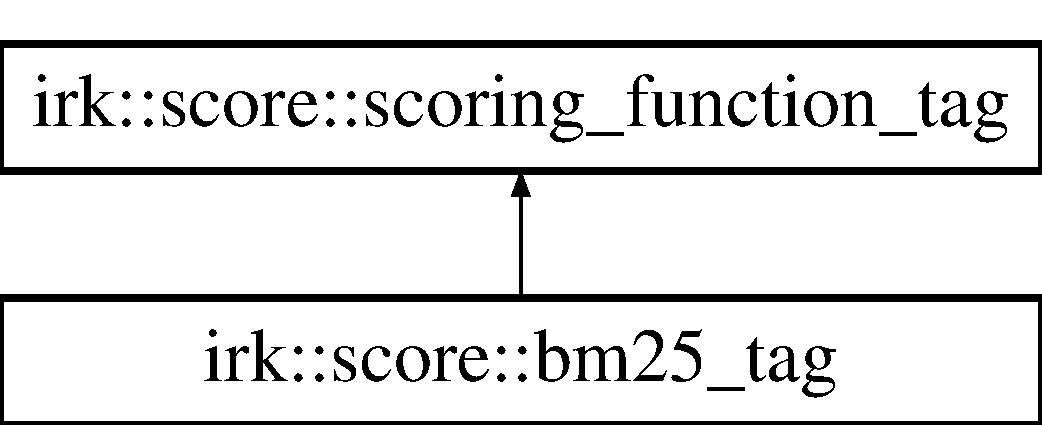
\includegraphics[height=2.000000cm]{structirk_1_1score_1_1bm25__tag}
\end{center}
\end{figure}
\subsection*{Public Member Functions}
\begin{DoxyCompactItemize}
\item 
\mbox{\hyperlink{structirk_1_1score_1_1bm25__tag_a3575a5c838ad5a235198d525e665e0f1}{operator std\+::string}} () override
\end{DoxyCompactItemize}


\subsection{Member Function Documentation}
\mbox{\Hypertarget{structirk_1_1score_1_1bm25__tag_a3575a5c838ad5a235198d525e665e0f1}\label{structirk_1_1score_1_1bm25__tag_a3575a5c838ad5a235198d525e665e0f1}} 
\index{irk\+::score\+::bm25\+\_\+tag@{irk\+::score\+::bm25\+\_\+tag}!operator std\+::string@{operator std\+::string}}
\index{operator std\+::string@{operator std\+::string}!irk\+::score\+::bm25\+\_\+tag@{irk\+::score\+::bm25\+\_\+tag}}
\subsubsection{\texorpdfstring{operator std\+::string()}{operator std::string()}}
{\footnotesize\ttfamily irk\+::score\+::bm25\+\_\+tag\+::operator std\+::string (\begin{DoxyParamCaption}{ }\end{DoxyParamCaption})\hspace{0.3cm}{\ttfamily [inline]}, {\ttfamily [explicit]}, {\ttfamily [override]}, {\ttfamily [virtual]}}



Implements \mbox{\hyperlink{structirk_1_1score_1_1scoring__function__tag_a718047dd6d5a9edd7b76ec55f2599c49}{irk\+::score\+::scoring\+\_\+function\+\_\+tag}}.



The documentation for this struct was generated from the following file\+:\begin{DoxyCompactItemize}
\item 
include/irkit/\mbox{\hyperlink{score_8hpp}{score.\+hpp}}\end{DoxyCompactItemize}

\hypertarget{structbody__writer}{}\section{body\+\_\+writer Struct Reference}
\label{structbody__writer}\index{body\+\_\+writer@{body\+\_\+writer}}
\subsection*{Public Member Functions}
\begin{DoxyCompactItemize}
\item 
void \mbox{\hyperlink{structbody__writer_a6050dfcfb3991a16c29775c3f1fcba81}{operator()}} (const std\+::string \&content)
\end{DoxyCompactItemize}
\subsection*{Public Attributes}
\begin{DoxyCompactItemize}
\item 
bool \mbox{\hyperlink{structbody__writer_a6df150a131f73f0174993cf6c496312f}{lowercase}}
\item 
\mbox{\hyperlink{structirk_1_1porter2_1_1SN__env}{irk\+::porter2\+::\+S\+N\+\_\+env}} $\ast$ \mbox{\hyperlink{structbody__writer_a4bf261cc5299b2eae268e0ed61bb17d6}{z}}
\end{DoxyCompactItemize}


\subsection{Member Function Documentation}
\mbox{\Hypertarget{structbody__writer_a6050dfcfb3991a16c29775c3f1fcba81}\label{structbody__writer_a6050dfcfb3991a16c29775c3f1fcba81}} 
\index{body\+\_\+writer@{body\+\_\+writer}!operator()@{operator()}}
\index{operator()@{operator()}!body\+\_\+writer@{body\+\_\+writer}}
\subsubsection{\texorpdfstring{operator()()}{operator()()}}
{\footnotesize\ttfamily void body\+\_\+writer\+::operator() (\begin{DoxyParamCaption}\item[{const std\+::string \&}]{content }\end{DoxyParamCaption})\hspace{0.3cm}{\ttfamily [inline]}}



\subsection{Member Data Documentation}
\mbox{\Hypertarget{structbody__writer_a6df150a131f73f0174993cf6c496312f}\label{structbody__writer_a6df150a131f73f0174993cf6c496312f}} 
\index{body\+\_\+writer@{body\+\_\+writer}!lowercase@{lowercase}}
\index{lowercase@{lowercase}!body\+\_\+writer@{body\+\_\+writer}}
\subsubsection{\texorpdfstring{lowercase}{lowercase}}
{\footnotesize\ttfamily bool body\+\_\+writer\+::lowercase}

\mbox{\Hypertarget{structbody__writer_a4bf261cc5299b2eae268e0ed61bb17d6}\label{structbody__writer_a4bf261cc5299b2eae268e0ed61bb17d6}} 
\index{body\+\_\+writer@{body\+\_\+writer}!z@{z}}
\index{z@{z}!body\+\_\+writer@{body\+\_\+writer}}
\subsubsection{\texorpdfstring{z}{z}}
{\footnotesize\ttfamily \mbox{\hyperlink{structirk_1_1porter2_1_1SN__env}{irk\+::porter2\+::\+S\+N\+\_\+env}}$\ast$ body\+\_\+writer\+::z}



The documentation for this struct was generated from the following file\+:\begin{DoxyCompactItemize}
\item 
src/\mbox{\hyperlink{irk-warc_8cpp}{irk-\/warc.\+cpp}}\end{DoxyCompactItemize}

\hypertarget{classcheck__fields}{}\section{check\+\_\+fields Class Reference}
\label{classcheck__fields}\index{check\+\_\+fields@{check\+\_\+fields}}
\subsection*{Public Member Functions}
\begin{DoxyCompactItemize}
\item 
\mbox{\hyperlink{classcheck__fields_a37a0409898667aad8601e57685252870}{check\+\_\+fields}} (const std\+::set$<$ char $>$ \&available\+\_\+fields)
\item 
std\+::string \mbox{\hyperlink{classcheck__fields_a7c9211374f47a59c3b796a1036bf3d96}{operator()}} (const std\+::string \&description)
\end{DoxyCompactItemize}


\subsection{Constructor \& Destructor Documentation}
\mbox{\Hypertarget{classcheck__fields_a37a0409898667aad8601e57685252870}\label{classcheck__fields_a37a0409898667aad8601e57685252870}} 
\index{check\+\_\+fields@{check\+\_\+fields}!check\+\_\+fields@{check\+\_\+fields}}
\index{check\+\_\+fields@{check\+\_\+fields}!check\+\_\+fields@{check\+\_\+fields}}
\subsubsection{\texorpdfstring{check\+\_\+fields()}{check\_fields()}}
{\footnotesize\ttfamily check\+\_\+fields\+::check\+\_\+fields (\begin{DoxyParamCaption}\item[{const std\+::set$<$ char $>$ \&}]{available\+\_\+fields }\end{DoxyParamCaption})\hspace{0.3cm}{\ttfamily [inline]}}



\subsection{Member Function Documentation}
\mbox{\Hypertarget{classcheck__fields_a7c9211374f47a59c3b796a1036bf3d96}\label{classcheck__fields_a7c9211374f47a59c3b796a1036bf3d96}} 
\index{check\+\_\+fields@{check\+\_\+fields}!operator()@{operator()}}
\index{operator()@{operator()}!check\+\_\+fields@{check\+\_\+fields}}
\subsubsection{\texorpdfstring{operator()()}{operator()()}}
{\footnotesize\ttfamily std\+::string check\+\_\+fields\+::operator() (\begin{DoxyParamCaption}\item[{const std\+::string \&}]{description }\end{DoxyParamCaption})\hspace{0.3cm}{\ttfamily [inline]}}



The documentation for this class was generated from the following file\+:\begin{DoxyCompactItemize}
\item 
src/\mbox{\hyperlink{irk-warc_8cpp}{irk-\/warc.\+cpp}}\end{DoxyCompactItemize}

\hypertarget{classirk_1_1columnar__reader}{}\section{irk\+:\+:columnar\+\_\+reader Class Reference}
\label{classirk_1_1columnar__reader}\index{irk\+::columnar\+\_\+reader@{irk\+::columnar\+\_\+reader}}


{\ttfamily \#include $<$column\+\_\+reader.\+hpp$>$}

\subsection*{Public Member Functions}
\begin{DoxyCompactItemize}
\item 
\mbox{\hyperlink{classirk_1_1columnar__reader}{columnar\+\_\+reader}} \& \mbox{\hyperlink{classirk_1_1columnar__reader_ac4d65bada006d0b99b569c15e6001a6e}{read\+\_\+header}} ()
\item 
\mbox{\hyperlink{classirk_1_1columnar__reader}{columnar\+\_\+reader}} \& \mbox{\hyperlink{classirk_1_1columnar__reader_a543757a48878cad7907736d1a2608bea}{next\+\_\+line}} ()
\item 
{\footnotesize template$<$class Accessor $>$ }\\std\+::string\+\_\+view \mbox{\hyperlink{classirk_1_1columnar__reader_aff87f04c5cc74aa6dadd0a4b150ce1db}{get}} (Accessor column) const
\item 
\mbox{\hyperlink{classirk_1_1columnar__reader_aad00b13b59559e7be029d7cc0766cd0f}{operator bool}} () const
\end{DoxyCompactItemize}


\subsection{Member Function Documentation}
\mbox{\Hypertarget{classirk_1_1columnar__reader_aff87f04c5cc74aa6dadd0a4b150ce1db}\label{classirk_1_1columnar__reader_aff87f04c5cc74aa6dadd0a4b150ce1db}} 
\index{irk\+::columnar\+\_\+reader@{irk\+::columnar\+\_\+reader}!get@{get}}
\index{get@{get}!irk\+::columnar\+\_\+reader@{irk\+::columnar\+\_\+reader}}
\subsubsection{\texorpdfstring{get()}{get()}}
{\footnotesize\ttfamily template$<$class Accessor $>$ \\
std\+::string\+\_\+view irk\+::columnar\+\_\+reader\+::get (\begin{DoxyParamCaption}\item[{Accessor}]{column }\end{DoxyParamCaption}) const\hspace{0.3cm}{\ttfamily [inline]}}

\mbox{\Hypertarget{classirk_1_1columnar__reader_a543757a48878cad7907736d1a2608bea}\label{classirk_1_1columnar__reader_a543757a48878cad7907736d1a2608bea}} 
\index{irk\+::columnar\+\_\+reader@{irk\+::columnar\+\_\+reader}!next\+\_\+line@{next\+\_\+line}}
\index{next\+\_\+line@{next\+\_\+line}!irk\+::columnar\+\_\+reader@{irk\+::columnar\+\_\+reader}}
\subsubsection{\texorpdfstring{next\+\_\+line()}{next\_line()}}
{\footnotesize\ttfamily \mbox{\hyperlink{classirk_1_1columnar__reader}{columnar\+\_\+reader}}\& irk\+::columnar\+\_\+reader\+::next\+\_\+line (\begin{DoxyParamCaption}{ }\end{DoxyParamCaption})\hspace{0.3cm}{\ttfamily [inline]}}

\mbox{\Hypertarget{classirk_1_1columnar__reader_aad00b13b59559e7be029d7cc0766cd0f}\label{classirk_1_1columnar__reader_aad00b13b59559e7be029d7cc0766cd0f}} 
\index{irk\+::columnar\+\_\+reader@{irk\+::columnar\+\_\+reader}!operator bool@{operator bool}}
\index{operator bool@{operator bool}!irk\+::columnar\+\_\+reader@{irk\+::columnar\+\_\+reader}}
\subsubsection{\texorpdfstring{operator bool()}{operator bool()}}
{\footnotesize\ttfamily irk\+::columnar\+\_\+reader\+::operator bool (\begin{DoxyParamCaption}{ }\end{DoxyParamCaption}) const\hspace{0.3cm}{\ttfamily [inline]}}

\mbox{\Hypertarget{classirk_1_1columnar__reader_ac4d65bada006d0b99b569c15e6001a6e}\label{classirk_1_1columnar__reader_ac4d65bada006d0b99b569c15e6001a6e}} 
\index{irk\+::columnar\+\_\+reader@{irk\+::columnar\+\_\+reader}!read\+\_\+header@{read\+\_\+header}}
\index{read\+\_\+header@{read\+\_\+header}!irk\+::columnar\+\_\+reader@{irk\+::columnar\+\_\+reader}}
\subsubsection{\texorpdfstring{read\+\_\+header()}{read\_header()}}
{\footnotesize\ttfamily \mbox{\hyperlink{classirk_1_1columnar__reader}{columnar\+\_\+reader}}\& irk\+::columnar\+\_\+reader\+::read\+\_\+header (\begin{DoxyParamCaption}{ }\end{DoxyParamCaption})\hspace{0.3cm}{\ttfamily [inline]}}



The documentation for this class was generated from the following file\+:\begin{DoxyCompactItemize}
\item 
include/irkit/\mbox{\hyperlink{column__reader_8hpp}{column\+\_\+reader.\+hpp}}\end{DoxyCompactItemize}

\hypertarget{classirk_1_1columnar__row}{}\section{irk\+:\+:columnar\+\_\+row$<$ types $>$ Class Template Reference}
\label{classirk_1_1columnar__row}\index{irk\+::columnar\+\_\+row$<$ types $>$@{irk\+::columnar\+\_\+row$<$ types $>$}}


{\ttfamily \#include $<$column\+\_\+reader.\+hpp$>$}



The documentation for this class was generated from the following file\+:\begin{DoxyCompactItemize}
\item 
include/irkit/\mbox{\hyperlink{column__reader_8hpp}{column\+\_\+reader.\+hpp}}\end{DoxyCompactItemize}

\hypertarget{classirk_1_1compact__table}{}\section{irk\+:\+:compact\+\_\+table$<$ T, Codec $>$ Class Template Reference}
\label{classirk_1_1compact__table}\index{irk\+::compact\+\_\+table$<$ T, Codec $>$@{irk\+::compact\+\_\+table$<$ T, Codec $>$}}


Fast-\/access compressed array.  




{\ttfamily \#include $<$compacttable.\+hpp$>$}

\subsection*{Public Types}
\begin{DoxyCompactItemize}
\item 
using \mbox{\hyperlink{classirk_1_1compact__table_a1c0c667110b82f790a0c0088e53ff461}{value\+\_\+type}} = typename Codec\+::value\+\_\+type
\end{DoxyCompactItemize}
\subsection*{Public Member Functions}
\begin{DoxyCompactItemize}
\item 
\mbox{\hyperlink{classirk_1_1compact__table_a7a5ea0a767cf151a37639532e36712f3}{compact\+\_\+table}} (fs\+::path file)
\item 
\mbox{\hyperlink{classirk_1_1compact__table_a3400a8843f4c286fd49417eeca2c9e74}{compact\+\_\+table}} (const std\+::vector$<$ T $>$ \&values, bool delta\+\_\+encoded=false, std\+::uint32\+\_\+t block\+\_\+size=256)
\item 
std\+::size\+\_\+t \mbox{\hyperlink{classirk_1_1compact__table_a7b0ae00675c32fcc1e7804f1ad3ab3ad}{operator\mbox{[}$\,$\mbox{]}}} (std\+::size\+\_\+t term\+\_\+id)
\item 
std\+::size\+\_\+t \mbox{\hyperlink{classirk_1_1compact__table_ac80ecca694d256e4f3c5c29e98900ccc}{operator\mbox{[}$\,$\mbox{]}}} (std\+::size\+\_\+t term\+\_\+id) const
\item 
const char $\ast$ \mbox{\hyperlink{classirk_1_1compact__table_a33d2d55685fe583f89521c2ca9797973}{data}} ()
\item 
const \mbox{\hyperlink{structirk_1_1compact__table__header}{compact\+\_\+table\+\_\+header}} $\ast$ \mbox{\hyperlink{classirk_1_1compact__table_ac5b6d8b0f58abd180ebd0d57396aa7ac}{header}} () const
\item 
std\+::size\+\_\+t \mbox{\hyperlink{classirk_1_1compact__table_adb0104bee02709980c7a7f9cd3a7719e}{size}} () const
\item 
bool \mbox{\hyperlink{classirk_1_1compact__table_ae2947a995621e70e7e7c533e30a0e043}{operator==}} (const \mbox{\hyperlink{classirk_1_1compact__table}{compact\+\_\+table}}$<$ T, Codec $>$ \&rhs)
\end{DoxyCompactItemize}
\subsection*{Protected Attributes}
\begin{DoxyCompactItemize}
\item 
Codec \mbox{\hyperlink{classirk_1_1compact__table_a780f480df7180c7b750907dc1954e741}{codec\+\_\+}}
\item 
std\+::vector$<$ char $>$ \mbox{\hyperlink{classirk_1_1compact__table_adf7928280ada85abfdf858586aeadb78}{data\+\_\+}}
\end{DoxyCompactItemize}
\subsection*{Friends}
\begin{DoxyCompactItemize}
\item 
std\+::ostream \& \mbox{\hyperlink{classirk_1_1compact__table_aabbde77b5cb5faeef5fe72eff9624aa5}{operator$<$$<$}} (std\+::ostream \&, const \mbox{\hyperlink{classirk_1_1compact__table}{compact\+\_\+table}}$<$ T, Codec $>$ \&)
\end{DoxyCompactItemize}


\subsection{Detailed Description}
\subsubsection*{template$<$class T, class Codec = coding\+::varbyte\+\_\+codec$<$\+T$>$$>$\newline
class irk\+::compact\+\_\+table$<$ T, Codec $>$}

Fast-\/access compressed array. 


\begin{DoxyTemplParams}{Template Parameters}
{\em T} & the type of the stored values \\
\hline
{\em Codec} & a codec that encodes values of type {\ttfamily T}\\
\hline
\end{DoxyTemplParams}
This is a compressed table indexed with consecutive integers between {\ttfamily 0} and {\ttfamily size -\/ 1}. T\+O\+DO\+: describe implmentation.

\begin{DoxyAuthor}{Author}
Michal Siedlaczek 
\end{DoxyAuthor}


\subsection{Member Typedef Documentation}
\mbox{\Hypertarget{classirk_1_1compact__table_a1c0c667110b82f790a0c0088e53ff461}\label{classirk_1_1compact__table_a1c0c667110b82f790a0c0088e53ff461}} 
\index{irk\+::compact\+\_\+table@{irk\+::compact\+\_\+table}!value\+\_\+type@{value\+\_\+type}}
\index{value\+\_\+type@{value\+\_\+type}!irk\+::compact\+\_\+table@{irk\+::compact\+\_\+table}}
\subsubsection{\texorpdfstring{value\+\_\+type}{value\_type}}
{\footnotesize\ttfamily template$<$class T, class Codec = coding\+::varbyte\+\_\+codec$<$\+T$>$$>$ \\
using \mbox{\hyperlink{classirk_1_1compact__table}{irk\+::compact\+\_\+table}}$<$ T, Codec $>$\+::\mbox{\hyperlink{classirk_1_1compact__table_a1c0c667110b82f790a0c0088e53ff461}{value\+\_\+type}} =  typename Codec\+::value\+\_\+type}



\subsection{Constructor \& Destructor Documentation}
\mbox{\Hypertarget{classirk_1_1compact__table_a7a5ea0a767cf151a37639532e36712f3}\label{classirk_1_1compact__table_a7a5ea0a767cf151a37639532e36712f3}} 
\index{irk\+::compact\+\_\+table@{irk\+::compact\+\_\+table}!compact\+\_\+table@{compact\+\_\+table}}
\index{compact\+\_\+table@{compact\+\_\+table}!irk\+::compact\+\_\+table@{irk\+::compact\+\_\+table}}
\subsubsection{\texorpdfstring{compact\+\_\+table()}{compact\_table()}\hspace{0.1cm}{\footnotesize\ttfamily [1/2]}}
{\footnotesize\ttfamily template$<$class T, class Codec = coding\+::varbyte\+\_\+codec$<$\+T$>$$>$ \\
\mbox{\hyperlink{classirk_1_1compact__table}{irk\+::compact\+\_\+table}}$<$ T, Codec $>$\+::\mbox{\hyperlink{classirk_1_1compact__table}{compact\+\_\+table}} (\begin{DoxyParamCaption}\item[{fs\+::path}]{file }\end{DoxyParamCaption})\hspace{0.3cm}{\ttfamily [inline]}}

\mbox{\Hypertarget{classirk_1_1compact__table_a3400a8843f4c286fd49417eeca2c9e74}\label{classirk_1_1compact__table_a3400a8843f4c286fd49417eeca2c9e74}} 
\index{irk\+::compact\+\_\+table@{irk\+::compact\+\_\+table}!compact\+\_\+table@{compact\+\_\+table}}
\index{compact\+\_\+table@{compact\+\_\+table}!irk\+::compact\+\_\+table@{irk\+::compact\+\_\+table}}
\subsubsection{\texorpdfstring{compact\+\_\+table()}{compact\_table()}\hspace{0.1cm}{\footnotesize\ttfamily [2/2]}}
{\footnotesize\ttfamily template$<$class T, class Codec = coding\+::varbyte\+\_\+codec$<$\+T$>$$>$ \\
\mbox{\hyperlink{classirk_1_1compact__table}{irk\+::compact\+\_\+table}}$<$ T, Codec $>$\+::\mbox{\hyperlink{classirk_1_1compact__table}{compact\+\_\+table}} (\begin{DoxyParamCaption}\item[{const std\+::vector$<$ T $>$ \&}]{values,  }\item[{bool}]{delta\+\_\+encoded = {\ttfamily false},  }\item[{std\+::uint32\+\_\+t}]{block\+\_\+size = {\ttfamily 256} }\end{DoxyParamCaption})\hspace{0.3cm}{\ttfamily [inline]}}



\subsection{Member Function Documentation}
\mbox{\Hypertarget{classirk_1_1compact__table_a33d2d55685fe583f89521c2ca9797973}\label{classirk_1_1compact__table_a33d2d55685fe583f89521c2ca9797973}} 
\index{irk\+::compact\+\_\+table@{irk\+::compact\+\_\+table}!data@{data}}
\index{data@{data}!irk\+::compact\+\_\+table@{irk\+::compact\+\_\+table}}
\subsubsection{\texorpdfstring{data()}{data()}}
{\footnotesize\ttfamily template$<$class T, class Codec = coding\+::varbyte\+\_\+codec$<$\+T$>$$>$ \\
const char$\ast$ \mbox{\hyperlink{classirk_1_1compact__table}{irk\+::compact\+\_\+table}}$<$ T, Codec $>$\+::data (\begin{DoxyParamCaption}{ }\end{DoxyParamCaption})\hspace{0.3cm}{\ttfamily [inline]}}

\mbox{\Hypertarget{classirk_1_1compact__table_ac5b6d8b0f58abd180ebd0d57396aa7ac}\label{classirk_1_1compact__table_ac5b6d8b0f58abd180ebd0d57396aa7ac}} 
\index{irk\+::compact\+\_\+table@{irk\+::compact\+\_\+table}!header@{header}}
\index{header@{header}!irk\+::compact\+\_\+table@{irk\+::compact\+\_\+table}}
\subsubsection{\texorpdfstring{header()}{header()}}
{\footnotesize\ttfamily template$<$class T, class Codec = coding\+::varbyte\+\_\+codec$<$\+T$>$$>$ \\
const \mbox{\hyperlink{structirk_1_1compact__table__header}{compact\+\_\+table\+\_\+header}}$\ast$ \mbox{\hyperlink{classirk_1_1compact__table}{irk\+::compact\+\_\+table}}$<$ T, Codec $>$\+::header (\begin{DoxyParamCaption}{ }\end{DoxyParamCaption}) const\hspace{0.3cm}{\ttfamily [inline]}}

\mbox{\Hypertarget{classirk_1_1compact__table_ae2947a995621e70e7e7c533e30a0e043}\label{classirk_1_1compact__table_ae2947a995621e70e7e7c533e30a0e043}} 
\index{irk\+::compact\+\_\+table@{irk\+::compact\+\_\+table}!operator==@{operator==}}
\index{operator==@{operator==}!irk\+::compact\+\_\+table@{irk\+::compact\+\_\+table}}
\subsubsection{\texorpdfstring{operator==()}{operator==()}}
{\footnotesize\ttfamily template$<$class T, class Codec = coding\+::varbyte\+\_\+codec$<$\+T$>$$>$ \\
bool \mbox{\hyperlink{classirk_1_1compact__table}{irk\+::compact\+\_\+table}}$<$ T, Codec $>$\+::operator== (\begin{DoxyParamCaption}\item[{const \mbox{\hyperlink{classirk_1_1compact__table}{compact\+\_\+table}}$<$ T, Codec $>$ \&}]{rhs }\end{DoxyParamCaption})\hspace{0.3cm}{\ttfamily [inline]}}

\mbox{\Hypertarget{classirk_1_1compact__table_a7b0ae00675c32fcc1e7804f1ad3ab3ad}\label{classirk_1_1compact__table_a7b0ae00675c32fcc1e7804f1ad3ab3ad}} 
\index{irk\+::compact\+\_\+table@{irk\+::compact\+\_\+table}!operator\mbox{[}\mbox{]}@{operator[]}}
\index{operator\mbox{[}\mbox{]}@{operator[]}!irk\+::compact\+\_\+table@{irk\+::compact\+\_\+table}}
\subsubsection{\texorpdfstring{operator[]()}{operator[]()}\hspace{0.1cm}{\footnotesize\ttfamily [1/2]}}
{\footnotesize\ttfamily template$<$class T, class Codec = coding\+::varbyte\+\_\+codec$<$\+T$>$$>$ \\
std\+::size\+\_\+t \mbox{\hyperlink{classirk_1_1compact__table}{irk\+::compact\+\_\+table}}$<$ T, Codec $>$\+::operator\mbox{[}$\,$\mbox{]} (\begin{DoxyParamCaption}\item[{std\+::size\+\_\+t}]{term\+\_\+id }\end{DoxyParamCaption})\hspace{0.3cm}{\ttfamily [inline]}}

\mbox{\Hypertarget{classirk_1_1compact__table_ac80ecca694d256e4f3c5c29e98900ccc}\label{classirk_1_1compact__table_ac80ecca694d256e4f3c5c29e98900ccc}} 
\index{irk\+::compact\+\_\+table@{irk\+::compact\+\_\+table}!operator\mbox{[}\mbox{]}@{operator[]}}
\index{operator\mbox{[}\mbox{]}@{operator[]}!irk\+::compact\+\_\+table@{irk\+::compact\+\_\+table}}
\subsubsection{\texorpdfstring{operator[]()}{operator[]()}\hspace{0.1cm}{\footnotesize\ttfamily [2/2]}}
{\footnotesize\ttfamily template$<$class T, class Codec = coding\+::varbyte\+\_\+codec$<$\+T$>$$>$ \\
std\+::size\+\_\+t \mbox{\hyperlink{classirk_1_1compact__table}{irk\+::compact\+\_\+table}}$<$ T, Codec $>$\+::operator\mbox{[}$\,$\mbox{]} (\begin{DoxyParamCaption}\item[{std\+::size\+\_\+t}]{term\+\_\+id }\end{DoxyParamCaption}) const\hspace{0.3cm}{\ttfamily [inline]}}

\mbox{\Hypertarget{classirk_1_1compact__table_adb0104bee02709980c7a7f9cd3a7719e}\label{classirk_1_1compact__table_adb0104bee02709980c7a7f9cd3a7719e}} 
\index{irk\+::compact\+\_\+table@{irk\+::compact\+\_\+table}!size@{size}}
\index{size@{size}!irk\+::compact\+\_\+table@{irk\+::compact\+\_\+table}}
\subsubsection{\texorpdfstring{size()}{size()}}
{\footnotesize\ttfamily template$<$class T, class Codec = coding\+::varbyte\+\_\+codec$<$\+T$>$$>$ \\
std\+::size\+\_\+t \mbox{\hyperlink{classirk_1_1compact__table}{irk\+::compact\+\_\+table}}$<$ T, Codec $>$\+::size (\begin{DoxyParamCaption}{ }\end{DoxyParamCaption}) const\hspace{0.3cm}{\ttfamily [inline]}}



\subsection{Friends And Related Function Documentation}
\mbox{\Hypertarget{classirk_1_1compact__table_aabbde77b5cb5faeef5fe72eff9624aa5}\label{classirk_1_1compact__table_aabbde77b5cb5faeef5fe72eff9624aa5}} 
\index{irk\+::compact\+\_\+table@{irk\+::compact\+\_\+table}!operator$<$$<$@{operator$<$$<$}}
\index{operator$<$$<$@{operator$<$$<$}!irk\+::compact\+\_\+table@{irk\+::compact\+\_\+table}}
\subsubsection{\texorpdfstring{operator$<$$<$}{operator<<}}
{\footnotesize\ttfamily template$<$class T, class Codec = coding\+::varbyte\+\_\+codec$<$\+T$>$$>$ \\
std\+::ostream\& operator$<$$<$ (\begin{DoxyParamCaption}\item[{std\+::ostream \&}]{out,  }\item[{const \mbox{\hyperlink{classirk_1_1compact__table}{compact\+\_\+table}}$<$ T, Codec $>$ \&}]{offset\+\_\+table }\end{DoxyParamCaption})\hspace{0.3cm}{\ttfamily [friend]}}



\subsection{Member Data Documentation}
\mbox{\Hypertarget{classirk_1_1compact__table_a780f480df7180c7b750907dc1954e741}\label{classirk_1_1compact__table_a780f480df7180c7b750907dc1954e741}} 
\index{irk\+::compact\+\_\+table@{irk\+::compact\+\_\+table}!codec\+\_\+@{codec\+\_\+}}
\index{codec\+\_\+@{codec\+\_\+}!irk\+::compact\+\_\+table@{irk\+::compact\+\_\+table}}
\subsubsection{\texorpdfstring{codec\+\_\+}{codec\_}}
{\footnotesize\ttfamily template$<$class T, class Codec = coding\+::varbyte\+\_\+codec$<$\+T$>$$>$ \\
Codec \mbox{\hyperlink{classirk_1_1compact__table}{irk\+::compact\+\_\+table}}$<$ T, Codec $>$\+::codec\+\_\+\hspace{0.3cm}{\ttfamily [protected]}}

\mbox{\Hypertarget{classirk_1_1compact__table_adf7928280ada85abfdf858586aeadb78}\label{classirk_1_1compact__table_adf7928280ada85abfdf858586aeadb78}} 
\index{irk\+::compact\+\_\+table@{irk\+::compact\+\_\+table}!data\+\_\+@{data\+\_\+}}
\index{data\+\_\+@{data\+\_\+}!irk\+::compact\+\_\+table@{irk\+::compact\+\_\+table}}
\subsubsection{\texorpdfstring{data\+\_\+}{data\_}}
{\footnotesize\ttfamily template$<$class T, class Codec = coding\+::varbyte\+\_\+codec$<$\+T$>$$>$ \\
std\+::vector$<$char$>$ \mbox{\hyperlink{classirk_1_1compact__table}{irk\+::compact\+\_\+table}}$<$ T, Codec $>$\+::data\+\_\+\hspace{0.3cm}{\ttfamily [protected]}}



The documentation for this class was generated from the following file\+:\begin{DoxyCompactItemize}
\item 
include/irkit/\mbox{\hyperlink{compacttable_8hpp}{compacttable.\+hpp}}\end{DoxyCompactItemize}

\hypertarget{structirk_1_1compact__table__header}{}\section{irk\+:\+:compact\+\_\+table\+\_\+header Struct Reference}
\label{structirk_1_1compact__table__header}\index{irk\+::compact\+\_\+table\+\_\+header@{irk\+::compact\+\_\+table\+\_\+header}}


{\ttfamily \#include $<$compacttable.\+hpp$>$}

\subsection*{Public Attributes}
\begin{DoxyCompactItemize}
\item 
std\+::uint32\+\_\+t \mbox{\hyperlink{structirk_1_1compact__table__header_a56cc3abb7d6c177bf6ddfbb4a1607281}{count}} = 0
\item 
std\+::uint32\+\_\+t \mbox{\hyperlink{structirk_1_1compact__table__header_aa550cf8ef026351eaadad254f7fbed59}{block\+\_\+size}} = 0
\item 
std\+::uint32\+\_\+t \mbox{\hyperlink{structirk_1_1compact__table__header_ae76b0ba32ba8873575f480e3148f1738}{flags}} = \mbox{\hyperlink{structirk_1_1CompactTableHeaderFlags_a18debbc227dbcb7726817a08b541e5e0}{Compact\+Table\+Header\+Flags\+::\+Default}}
\end{DoxyCompactItemize}


\subsection{Member Data Documentation}
\mbox{\Hypertarget{structirk_1_1compact__table__header_aa550cf8ef026351eaadad254f7fbed59}\label{structirk_1_1compact__table__header_aa550cf8ef026351eaadad254f7fbed59}} 
\index{irk\+::compact\+\_\+table\+\_\+header@{irk\+::compact\+\_\+table\+\_\+header}!block\+\_\+size@{block\+\_\+size}}
\index{block\+\_\+size@{block\+\_\+size}!irk\+::compact\+\_\+table\+\_\+header@{irk\+::compact\+\_\+table\+\_\+header}}
\subsubsection{\texorpdfstring{block\+\_\+size}{block\_size}}
{\footnotesize\ttfamily std\+::uint32\+\_\+t irk\+::compact\+\_\+table\+\_\+header\+::block\+\_\+size = 0}

\mbox{\Hypertarget{structirk_1_1compact__table__header_a56cc3abb7d6c177bf6ddfbb4a1607281}\label{structirk_1_1compact__table__header_a56cc3abb7d6c177bf6ddfbb4a1607281}} 
\index{irk\+::compact\+\_\+table\+\_\+header@{irk\+::compact\+\_\+table\+\_\+header}!count@{count}}
\index{count@{count}!irk\+::compact\+\_\+table\+\_\+header@{irk\+::compact\+\_\+table\+\_\+header}}
\subsubsection{\texorpdfstring{count}{count}}
{\footnotesize\ttfamily std\+::uint32\+\_\+t irk\+::compact\+\_\+table\+\_\+header\+::count = 0}

\mbox{\Hypertarget{structirk_1_1compact__table__header_ae76b0ba32ba8873575f480e3148f1738}\label{structirk_1_1compact__table__header_ae76b0ba32ba8873575f480e3148f1738}} 
\index{irk\+::compact\+\_\+table\+\_\+header@{irk\+::compact\+\_\+table\+\_\+header}!flags@{flags}}
\index{flags@{flags}!irk\+::compact\+\_\+table\+\_\+header@{irk\+::compact\+\_\+table\+\_\+header}}
\subsubsection{\texorpdfstring{flags}{flags}}
{\footnotesize\ttfamily std\+::uint32\+\_\+t irk\+::compact\+\_\+table\+\_\+header\+::flags = \mbox{\hyperlink{structirk_1_1CompactTableHeaderFlags_a18debbc227dbcb7726817a08b541e5e0}{Compact\+Table\+Header\+Flags\+::\+Default}}}



The documentation for this struct was generated from the following file\+:\begin{DoxyCompactItemize}
\item 
include/irkit/\mbox{\hyperlink{compacttable_8hpp}{compacttable.\+hpp}}\end{DoxyCompactItemize}

\hypertarget{structirk_1_1compact__table__leader}{}\section{irk\+:\+:compact\+\_\+table\+\_\+leader Struct Reference}
\label{structirk_1_1compact__table__leader}\index{irk\+::compact\+\_\+table\+\_\+leader@{irk\+::compact\+\_\+table\+\_\+leader}}


{\ttfamily \#include $<$compacttable.\+hpp$>$}

\subsection*{Public Member Functions}
\begin{DoxyCompactItemize}
\item 
bool \mbox{\hyperlink{structirk_1_1compact__table__leader_ad96c038f67cec0df810807785ff0b175}{operator$<$}} (const \mbox{\hyperlink{structirk_1_1compact__table__leader}{compact\+\_\+table\+\_\+leader}} \&rhs) const
\end{DoxyCompactItemize}
\subsection*{Public Attributes}
\begin{DoxyCompactItemize}
\item 
std\+::uint32\+\_\+t \mbox{\hyperlink{structirk_1_1compact__table__leader_a250e11134b95bb0f559c531a56a548c5}{key}}
\item 
std\+::uint32\+\_\+t \mbox{\hyperlink{structirk_1_1compact__table__leader_aeeb27531e59da3a9be21627117fa0af3}{ptr}}
\end{DoxyCompactItemize}


\subsection{Member Function Documentation}
\mbox{\Hypertarget{structirk_1_1compact__table__leader_ad96c038f67cec0df810807785ff0b175}\label{structirk_1_1compact__table__leader_ad96c038f67cec0df810807785ff0b175}} 
\index{irk\+::compact\+\_\+table\+\_\+leader@{irk\+::compact\+\_\+table\+\_\+leader}!operator$<$@{operator$<$}}
\index{operator$<$@{operator$<$}!irk\+::compact\+\_\+table\+\_\+leader@{irk\+::compact\+\_\+table\+\_\+leader}}
\subsubsection{\texorpdfstring{operator$<$()}{operator<()}}
{\footnotesize\ttfamily bool irk\+::compact\+\_\+table\+\_\+leader\+::operator$<$ (\begin{DoxyParamCaption}\item[{const \mbox{\hyperlink{structirk_1_1compact__table__leader}{compact\+\_\+table\+\_\+leader}} \&}]{rhs }\end{DoxyParamCaption}) const\hspace{0.3cm}{\ttfamily [inline]}}



\subsection{Member Data Documentation}
\mbox{\Hypertarget{structirk_1_1compact__table__leader_a250e11134b95bb0f559c531a56a548c5}\label{structirk_1_1compact__table__leader_a250e11134b95bb0f559c531a56a548c5}} 
\index{irk\+::compact\+\_\+table\+\_\+leader@{irk\+::compact\+\_\+table\+\_\+leader}!key@{key}}
\index{key@{key}!irk\+::compact\+\_\+table\+\_\+leader@{irk\+::compact\+\_\+table\+\_\+leader}}
\subsubsection{\texorpdfstring{key}{key}}
{\footnotesize\ttfamily std\+::uint32\+\_\+t irk\+::compact\+\_\+table\+\_\+leader\+::key}

\mbox{\Hypertarget{structirk_1_1compact__table__leader_aeeb27531e59da3a9be21627117fa0af3}\label{structirk_1_1compact__table__leader_aeeb27531e59da3a9be21627117fa0af3}} 
\index{irk\+::compact\+\_\+table\+\_\+leader@{irk\+::compact\+\_\+table\+\_\+leader}!ptr@{ptr}}
\index{ptr@{ptr}!irk\+::compact\+\_\+table\+\_\+leader@{irk\+::compact\+\_\+table\+\_\+leader}}
\subsubsection{\texorpdfstring{ptr}{ptr}}
{\footnotesize\ttfamily std\+::uint32\+\_\+t irk\+::compact\+\_\+table\+\_\+leader\+::ptr}



The documentation for this struct was generated from the following file\+:\begin{DoxyCompactItemize}
\item 
include/irkit/\mbox{\hyperlink{compacttable_8hpp}{compacttable.\+hpp}}\end{DoxyCompactItemize}

\hypertarget{structirk_1_1CompactTableHeaderFlags}{}\section{irk\+:\+:Compact\+Table\+Header\+Flags Struct Reference}
\label{structirk_1_1CompactTableHeaderFlags}\index{irk\+::\+Compact\+Table\+Header\+Flags@{irk\+::\+Compact\+Table\+Header\+Flags}}


{\ttfamily \#include $<$compacttable.\+hpp$>$}

\subsection*{Static Public Attributes}
\begin{DoxyCompactItemize}
\item 
static const std\+::uint32\+\_\+t \mbox{\hyperlink{structirk_1_1CompactTableHeaderFlags_a18debbc227dbcb7726817a08b541e5e0}{Default}} = 0
\item 
static const std\+::uint32\+\_\+t \mbox{\hyperlink{structirk_1_1CompactTableHeaderFlags_af00ac402429458ce945d2fa2313f66bc}{Delta\+Encoding}} = 1
\end{DoxyCompactItemize}


\subsection{Member Data Documentation}
\mbox{\Hypertarget{structirk_1_1CompactTableHeaderFlags_a18debbc227dbcb7726817a08b541e5e0}\label{structirk_1_1CompactTableHeaderFlags_a18debbc227dbcb7726817a08b541e5e0}} 
\index{irk\+::\+Compact\+Table\+Header\+Flags@{irk\+::\+Compact\+Table\+Header\+Flags}!Default@{Default}}
\index{Default@{Default}!irk\+::\+Compact\+Table\+Header\+Flags@{irk\+::\+Compact\+Table\+Header\+Flags}}
\subsubsection{\texorpdfstring{Default}{Default}}
{\footnotesize\ttfamily const std\+::uint32\+\_\+t irk\+::\+Compact\+Table\+Header\+Flags\+::\+Default = 0\hspace{0.3cm}{\ttfamily [static]}}

\mbox{\Hypertarget{structirk_1_1CompactTableHeaderFlags_af00ac402429458ce945d2fa2313f66bc}\label{structirk_1_1CompactTableHeaderFlags_af00ac402429458ce945d2fa2313f66bc}} 
\index{irk\+::\+Compact\+Table\+Header\+Flags@{irk\+::\+Compact\+Table\+Header\+Flags}!Delta\+Encoding@{Delta\+Encoding}}
\index{Delta\+Encoding@{Delta\+Encoding}!irk\+::\+Compact\+Table\+Header\+Flags@{irk\+::\+Compact\+Table\+Header\+Flags}}
\subsubsection{\texorpdfstring{Delta\+Encoding}{DeltaEncoding}}
{\footnotesize\ttfamily const std\+::uint32\+\_\+t irk\+::\+Compact\+Table\+Header\+Flags\+::\+Delta\+Encoding = 1\hspace{0.3cm}{\ttfamily [static]}}



The documentation for this struct was generated from the following file\+:\begin{DoxyCompactItemize}
\item 
include/irkit/\mbox{\hyperlink{compacttable_8hpp}{compacttable.\+hpp}}\end{DoxyCompactItemize}

\hypertarget{structirk_1_1memory__view_1_1concept}{}\section{irk\+:\+:memory\+\_\+view\+:\+:concept Struct Reference}
\label{structirk_1_1memory__view_1_1concept}\index{irk\+::memory\+\_\+view\+::concept@{irk\+::memory\+\_\+view\+::concept}}


{\ttfamily \#include $<$memoryview.\+hpp$>$}

Inheritance diagram for irk\+:\+:memory\+\_\+view\+:\+:concept\+:\begin{figure}[H]
\begin{center}
\leavevmode
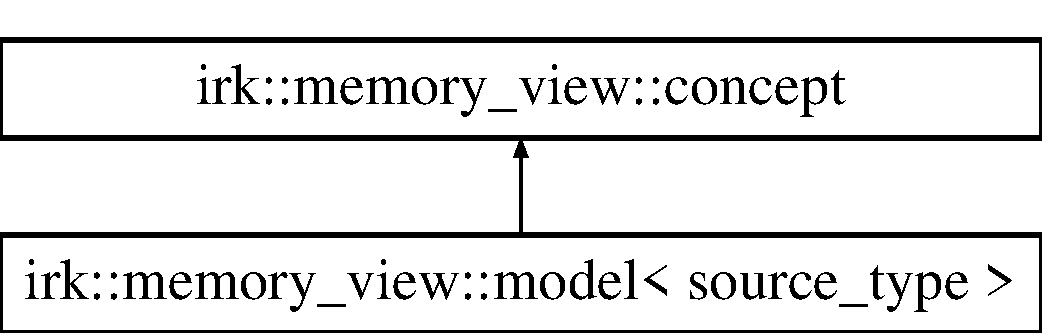
\includegraphics[height=2.000000cm]{structirk_1_1memory__view_1_1concept}
\end{center}
\end{figure}
\subsection*{Public Member Functions}
\begin{DoxyCompactItemize}
\item 
\mbox{\hyperlink{structirk_1_1memory__view_1_1concept_aae5e17857dc0611f3e09e9cbba9b0f57}{concept}} ()=default
\item 
\mbox{\hyperlink{structirk_1_1memory__view_1_1concept_a787ef96617397fef8d73a000a640528d}{concept}} (const \mbox{\hyperlink{structirk_1_1memory__view_1_1concept}{concept}} \&)=default
\item 
\mbox{\hyperlink{structirk_1_1memory__view_1_1concept_ae801147171040b17412295df48ea1275}{concept}} (\mbox{\hyperlink{structirk_1_1memory__view_1_1concept}{concept}} \&\&) noexcept=default
\item 
\mbox{\hyperlink{structirk_1_1memory__view_1_1concept}{concept}} \& \mbox{\hyperlink{structirk_1_1memory__view_1_1concept_a351a0e0485d2caf8de0f85678fa0de14}{operator=}} (const \mbox{\hyperlink{structirk_1_1memory__view_1_1concept}{concept}} \&)=default
\item 
\mbox{\hyperlink{structirk_1_1memory__view_1_1concept}{concept}} \& \mbox{\hyperlink{structirk_1_1memory__view_1_1concept_aff127d831dbed4a0e4f143e69ba639b0}{operator=}} (\mbox{\hyperlink{structirk_1_1memory__view_1_1concept}{concept}} \&\&) noexcept=default
\item 
virtual \mbox{\hyperlink{structirk_1_1memory__view_1_1concept_a970a71a31247472092552d2358968116}{$\sim$concept}} ()=default
\item 
virtual const char $\ast$ \mbox{\hyperlink{structirk_1_1memory__view_1_1concept_a9e124ac4016556f7cf7fd864dcc43a7c}{data}} () const =0
\item 
virtual gsl\+::index \mbox{\hyperlink{structirk_1_1memory__view_1_1concept_ae280e124e776a61562f6a97b2fa7d655}{size}} () const =0
\item 
virtual const char \& \mbox{\hyperlink{structirk_1_1memory__view_1_1concept_af36b274207af910870d186a747b9f9f1}{operator\mbox{[}$\,$\mbox{]}}} (std\+::ptrdiff\+\_\+t) const =0
\item 
virtual \mbox{\hyperlink{classirk_1_1memory__view}{memory\+\_\+view}} \mbox{\hyperlink{structirk_1_1memory__view_1_1concept_a9abcd2995563487390e941cf502b322c}{range}} (std\+::ptrdiff\+\_\+t first, std\+::ptrdiff\+\_\+t \mbox{\hyperlink{structirk_1_1memory__view_1_1concept_ae280e124e776a61562f6a97b2fa7d655}{size}}) const =0
\end{DoxyCompactItemize}


\subsection{Constructor \& Destructor Documentation}
\mbox{\Hypertarget{structirk_1_1memory__view_1_1concept_aae5e17857dc0611f3e09e9cbba9b0f57}\label{structirk_1_1memory__view_1_1concept_aae5e17857dc0611f3e09e9cbba9b0f57}} 
\index{irk\+::memory\+\_\+view\+::concept@{irk\+::memory\+\_\+view\+::concept}!concept@{concept}}
\index{concept@{concept}!irk\+::memory\+\_\+view\+::concept@{irk\+::memory\+\_\+view\+::concept}}
\subsubsection{\texorpdfstring{concept()}{concept()}\hspace{0.1cm}{\footnotesize\ttfamily [1/3]}}
{\footnotesize\ttfamily irk\+::memory\+\_\+view\+::concept\+::concept (\begin{DoxyParamCaption}{ }\end{DoxyParamCaption})\hspace{0.3cm}{\ttfamily [default]}}

\mbox{\Hypertarget{structirk_1_1memory__view_1_1concept_a787ef96617397fef8d73a000a640528d}\label{structirk_1_1memory__view_1_1concept_a787ef96617397fef8d73a000a640528d}} 
\index{irk\+::memory\+\_\+view\+::concept@{irk\+::memory\+\_\+view\+::concept}!concept@{concept}}
\index{concept@{concept}!irk\+::memory\+\_\+view\+::concept@{irk\+::memory\+\_\+view\+::concept}}
\subsubsection{\texorpdfstring{concept()}{concept()}\hspace{0.1cm}{\footnotesize\ttfamily [2/3]}}
{\footnotesize\ttfamily irk\+::memory\+\_\+view\+::concept\+::concept (\begin{DoxyParamCaption}\item[{const \mbox{\hyperlink{structirk_1_1memory__view_1_1concept}{concept}} \&}]{ }\end{DoxyParamCaption})\hspace{0.3cm}{\ttfamily [default]}}

\mbox{\Hypertarget{structirk_1_1memory__view_1_1concept_ae801147171040b17412295df48ea1275}\label{structirk_1_1memory__view_1_1concept_ae801147171040b17412295df48ea1275}} 
\index{irk\+::memory\+\_\+view\+::concept@{irk\+::memory\+\_\+view\+::concept}!concept@{concept}}
\index{concept@{concept}!irk\+::memory\+\_\+view\+::concept@{irk\+::memory\+\_\+view\+::concept}}
\subsubsection{\texorpdfstring{concept()}{concept()}\hspace{0.1cm}{\footnotesize\ttfamily [3/3]}}
{\footnotesize\ttfamily irk\+::memory\+\_\+view\+::concept\+::concept (\begin{DoxyParamCaption}\item[{\mbox{\hyperlink{structirk_1_1memory__view_1_1concept}{concept}} \&\&}]{ }\end{DoxyParamCaption})\hspace{0.3cm}{\ttfamily [default]}, {\ttfamily [noexcept]}}

\mbox{\Hypertarget{structirk_1_1memory__view_1_1concept_a970a71a31247472092552d2358968116}\label{structirk_1_1memory__view_1_1concept_a970a71a31247472092552d2358968116}} 
\index{irk\+::memory\+\_\+view\+::concept@{irk\+::memory\+\_\+view\+::concept}!````~concept@{$\sim$concept}}
\index{````~concept@{$\sim$concept}!irk\+::memory\+\_\+view\+::concept@{irk\+::memory\+\_\+view\+::concept}}
\subsubsection{\texorpdfstring{$\sim$concept()}{~concept()}}
{\footnotesize\ttfamily virtual irk\+::memory\+\_\+view\+::concept\+::$\sim$concept (\begin{DoxyParamCaption}{ }\end{DoxyParamCaption})\hspace{0.3cm}{\ttfamily [virtual]}, {\ttfamily [default]}}



\subsection{Member Function Documentation}
\mbox{\Hypertarget{structirk_1_1memory__view_1_1concept_a9e124ac4016556f7cf7fd864dcc43a7c}\label{structirk_1_1memory__view_1_1concept_a9e124ac4016556f7cf7fd864dcc43a7c}} 
\index{irk\+::memory\+\_\+view\+::concept@{irk\+::memory\+\_\+view\+::concept}!data@{data}}
\index{data@{data}!irk\+::memory\+\_\+view\+::concept@{irk\+::memory\+\_\+view\+::concept}}
\subsubsection{\texorpdfstring{data()}{data()}}
{\footnotesize\ttfamily virtual const char$\ast$ irk\+::memory\+\_\+view\+::concept\+::data (\begin{DoxyParamCaption}{ }\end{DoxyParamCaption}) const\hspace{0.3cm}{\ttfamily [pure virtual]}}



Implemented in \mbox{\hyperlink{classirk_1_1memory__view_1_1model_a5a7c432c460f99bd8b78c29ef6d44009}{irk\+::memory\+\_\+view\+::model$<$ source\+\_\+type $>$}}.

\mbox{\Hypertarget{structirk_1_1memory__view_1_1concept_a351a0e0485d2caf8de0f85678fa0de14}\label{structirk_1_1memory__view_1_1concept_a351a0e0485d2caf8de0f85678fa0de14}} 
\index{irk\+::memory\+\_\+view\+::concept@{irk\+::memory\+\_\+view\+::concept}!operator=@{operator=}}
\index{operator=@{operator=}!irk\+::memory\+\_\+view\+::concept@{irk\+::memory\+\_\+view\+::concept}}
\subsubsection{\texorpdfstring{operator=()}{operator=()}\hspace{0.1cm}{\footnotesize\ttfamily [1/2]}}
{\footnotesize\ttfamily \mbox{\hyperlink{structirk_1_1memory__view_1_1concept}{concept}}\& irk\+::memory\+\_\+view\+::concept\+::operator= (\begin{DoxyParamCaption}\item[{const \mbox{\hyperlink{structirk_1_1memory__view_1_1concept}{concept}} \&}]{ }\end{DoxyParamCaption})\hspace{0.3cm}{\ttfamily [default]}}

\mbox{\Hypertarget{structirk_1_1memory__view_1_1concept_aff127d831dbed4a0e4f143e69ba639b0}\label{structirk_1_1memory__view_1_1concept_aff127d831dbed4a0e4f143e69ba639b0}} 
\index{irk\+::memory\+\_\+view\+::concept@{irk\+::memory\+\_\+view\+::concept}!operator=@{operator=}}
\index{operator=@{operator=}!irk\+::memory\+\_\+view\+::concept@{irk\+::memory\+\_\+view\+::concept}}
\subsubsection{\texorpdfstring{operator=()}{operator=()}\hspace{0.1cm}{\footnotesize\ttfamily [2/2]}}
{\footnotesize\ttfamily \mbox{\hyperlink{structirk_1_1memory__view_1_1concept}{concept}}\& irk\+::memory\+\_\+view\+::concept\+::operator= (\begin{DoxyParamCaption}\item[{\mbox{\hyperlink{structirk_1_1memory__view_1_1concept}{concept}} \&\&}]{ }\end{DoxyParamCaption})\hspace{0.3cm}{\ttfamily [default]}, {\ttfamily [noexcept]}}

\mbox{\Hypertarget{structirk_1_1memory__view_1_1concept_af36b274207af910870d186a747b9f9f1}\label{structirk_1_1memory__view_1_1concept_af36b274207af910870d186a747b9f9f1}} 
\index{irk\+::memory\+\_\+view\+::concept@{irk\+::memory\+\_\+view\+::concept}!operator\mbox{[}\mbox{]}@{operator[]}}
\index{operator\mbox{[}\mbox{]}@{operator[]}!irk\+::memory\+\_\+view\+::concept@{irk\+::memory\+\_\+view\+::concept}}
\subsubsection{\texorpdfstring{operator[]()}{operator[]()}}
{\footnotesize\ttfamily virtual const char\& irk\+::memory\+\_\+view\+::concept\+::operator\mbox{[}$\,$\mbox{]} (\begin{DoxyParamCaption}\item[{std\+::ptrdiff\+\_\+t}]{ }\end{DoxyParamCaption}) const\hspace{0.3cm}{\ttfamily [pure virtual]}}



Implemented in \mbox{\hyperlink{classirk_1_1memory__view_1_1model_a8c54be09ffb8bd159e375d14a6f8218b}{irk\+::memory\+\_\+view\+::model$<$ source\+\_\+type $>$}}.

\mbox{\Hypertarget{structirk_1_1memory__view_1_1concept_a9abcd2995563487390e941cf502b322c}\label{structirk_1_1memory__view_1_1concept_a9abcd2995563487390e941cf502b322c}} 
\index{irk\+::memory\+\_\+view\+::concept@{irk\+::memory\+\_\+view\+::concept}!range@{range}}
\index{range@{range}!irk\+::memory\+\_\+view\+::concept@{irk\+::memory\+\_\+view\+::concept}}
\subsubsection{\texorpdfstring{range()}{range()}}
{\footnotesize\ttfamily virtual \mbox{\hyperlink{classirk_1_1memory__view}{memory\+\_\+view}} irk\+::memory\+\_\+view\+::concept\+::range (\begin{DoxyParamCaption}\item[{std\+::ptrdiff\+\_\+t}]{first,  }\item[{std\+::ptrdiff\+\_\+t}]{size }\end{DoxyParamCaption}) const\hspace{0.3cm}{\ttfamily [pure virtual]}}



Implemented in \mbox{\hyperlink{classirk_1_1memory__view_1_1model_aed67f637a1f0e7e31dcf039074861724}{irk\+::memory\+\_\+view\+::model$<$ source\+\_\+type $>$}}.

\mbox{\Hypertarget{structirk_1_1memory__view_1_1concept_ae280e124e776a61562f6a97b2fa7d655}\label{structirk_1_1memory__view_1_1concept_ae280e124e776a61562f6a97b2fa7d655}} 
\index{irk\+::memory\+\_\+view\+::concept@{irk\+::memory\+\_\+view\+::concept}!size@{size}}
\index{size@{size}!irk\+::memory\+\_\+view\+::concept@{irk\+::memory\+\_\+view\+::concept}}
\subsubsection{\texorpdfstring{size()}{size()}}
{\footnotesize\ttfamily virtual gsl\+::index irk\+::memory\+\_\+view\+::concept\+::size (\begin{DoxyParamCaption}{ }\end{DoxyParamCaption}) const\hspace{0.3cm}{\ttfamily [pure virtual]}}



Implemented in \mbox{\hyperlink{classirk_1_1memory__view_1_1model_a88bdaaf00f71b733bb67ea912ed78251}{irk\+::memory\+\_\+view\+::model$<$ source\+\_\+type $>$}}.



The documentation for this struct was generated from the following file\+:\begin{DoxyCompactItemize}
\item 
include/irkit/\mbox{\hyperlink{memoryview_8hpp}{memoryview.\+hpp}}\end{DoxyCompactItemize}

\hypertarget{structboost_1_1type__erasure_1_1concept__interface_3_01irk_1_1has__decode_3_01C_00_01T_01_4_00_01Base_00_01C_01_4}{}\section{boost\+:\+:type\+\_\+erasure\+:\+:concept\+\_\+interface$<$ irk\+:\+:has\+\_\+decode$<$ C, T $>$, Base, C $>$ Struct Template Reference}
\label{structboost_1_1type__erasure_1_1concept__interface_3_01irk_1_1has__decode_3_01C_00_01T_01_4_00_01Base_00_01C_01_4}\index{boost\+::type\+\_\+erasure\+::concept\+\_\+interface$<$ irk\+::has\+\_\+decode$<$ C, T $>$, Base, C $>$@{boost\+::type\+\_\+erasure\+::concept\+\_\+interface$<$ irk\+::has\+\_\+decode$<$ C, T $>$, Base, C $>$}}


{\ttfamily \#include $<$coding.\+hpp$>$}

Inheritance diagram for boost\+:\+:type\+\_\+erasure\+:\+:concept\+\_\+interface$<$ irk\+:\+:has\+\_\+decode$<$ C, T $>$, Base, C $>$\+:\begin{figure}[H]
\begin{center}
\leavevmode
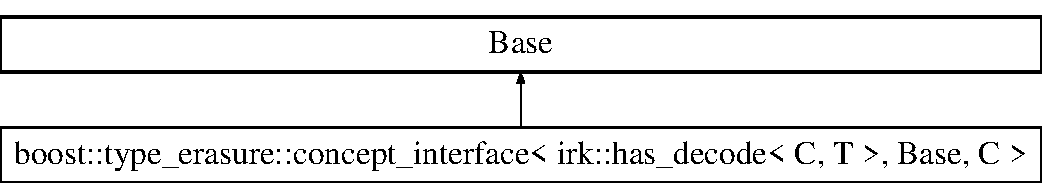
\includegraphics[height=2.000000cm]{structboost_1_1type__erasure_1_1concept__interface_3_01irk_1_1has__decode_3_01C_00_01T_01_4_00_01Base_00_01C_01_4}
\end{center}
\end{figure}
\subsection*{Public Types}
\begin{DoxyCompactItemize}
\item 
using \mbox{\hyperlink{structboost_1_1type__erasure_1_1concept__interface_3_01irk_1_1has__decode_3_01C_00_01T_01_4_00_01Base_00_01C_01_4_af45858ace775b12c9f2417325f99b268}{value\+\_\+type}} = T
\end{DoxyCompactItemize}
\subsection*{Public Member Functions}
\begin{DoxyCompactItemize}
\item 
std\+::streamsize \mbox{\hyperlink{structboost_1_1type__erasure_1_1concept__interface_3_01irk_1_1has__decode_3_01C_00_01T_01_4_00_01Base_00_01C_01_4_aeba766d79e975ed3869f9dee530e0bc5}{decode}} (std\+::istream \&source, typename as\+\_\+param$<$ Base, T \&$>$\+::type n) const
\end{DoxyCompactItemize}


\subsection{Member Typedef Documentation}
\mbox{\Hypertarget{structboost_1_1type__erasure_1_1concept__interface_3_01irk_1_1has__decode_3_01C_00_01T_01_4_00_01Base_00_01C_01_4_af45858ace775b12c9f2417325f99b268}\label{structboost_1_1type__erasure_1_1concept__interface_3_01irk_1_1has__decode_3_01C_00_01T_01_4_00_01Base_00_01C_01_4_af45858ace775b12c9f2417325f99b268}} 
\index{boost\+::type\+\_\+erasure\+::concept\+\_\+interface$<$ irk\+::has\+\_\+decode$<$ C, T $>$, Base, C $>$@{boost\+::type\+\_\+erasure\+::concept\+\_\+interface$<$ irk\+::has\+\_\+decode$<$ C, T $>$, Base, C $>$}!value\+\_\+type@{value\+\_\+type}}
\index{value\+\_\+type@{value\+\_\+type}!boost\+::type\+\_\+erasure\+::concept\+\_\+interface$<$ irk\+::has\+\_\+decode$<$ C, T $>$, Base, C $>$@{boost\+::type\+\_\+erasure\+::concept\+\_\+interface$<$ irk\+::has\+\_\+decode$<$ C, T $>$, Base, C $>$}}
\subsubsection{\texorpdfstring{value\+\_\+type}{value\_type}}
{\footnotesize\ttfamily template$<$class C , class T , class Base $>$ \\
using boost\+::type\+\_\+erasure\+::concept\+\_\+interface$<$ \mbox{\hyperlink{structirk_1_1has__decode}{irk\+::has\+\_\+decode}}$<$ C, T $>$, Base, C $>$\+::\mbox{\hyperlink{structboost_1_1type__erasure_1_1concept__interface_3_01irk_1_1has__decode_3_01C_00_01T_01_4_00_01Base_00_01C_01_4_af45858ace775b12c9f2417325f99b268}{value\+\_\+type}} =  T}



\subsection{Member Function Documentation}
\mbox{\Hypertarget{structboost_1_1type__erasure_1_1concept__interface_3_01irk_1_1has__decode_3_01C_00_01T_01_4_00_01Base_00_01C_01_4_aeba766d79e975ed3869f9dee530e0bc5}\label{structboost_1_1type__erasure_1_1concept__interface_3_01irk_1_1has__decode_3_01C_00_01T_01_4_00_01Base_00_01C_01_4_aeba766d79e975ed3869f9dee530e0bc5}} 
\index{boost\+::type\+\_\+erasure\+::concept\+\_\+interface$<$ irk\+::has\+\_\+decode$<$ C, T $>$, Base, C $>$@{boost\+::type\+\_\+erasure\+::concept\+\_\+interface$<$ irk\+::has\+\_\+decode$<$ C, T $>$, Base, C $>$}!decode@{decode}}
\index{decode@{decode}!boost\+::type\+\_\+erasure\+::concept\+\_\+interface$<$ irk\+::has\+\_\+decode$<$ C, T $>$, Base, C $>$@{boost\+::type\+\_\+erasure\+::concept\+\_\+interface$<$ irk\+::has\+\_\+decode$<$ C, T $>$, Base, C $>$}}
\subsubsection{\texorpdfstring{decode()}{decode()}}
{\footnotesize\ttfamily template$<$class C , class T , class Base $>$ \\
std\+::streamsize boost\+::type\+\_\+erasure\+::concept\+\_\+interface$<$ \mbox{\hyperlink{structirk_1_1has__decode}{irk\+::has\+\_\+decode}}$<$ C, T $>$, Base, C $>$\+::decode (\begin{DoxyParamCaption}\item[{std\+::istream \&}]{source,  }\item[{typename as\+\_\+param$<$ Base, T \&$>$\+::type}]{n }\end{DoxyParamCaption}) const\hspace{0.3cm}{\ttfamily [inline]}}



The documentation for this struct was generated from the following file\+:\begin{DoxyCompactItemize}
\item 
include/irkit/\mbox{\hyperlink{coding_8hpp}{coding.\+hpp}}\end{DoxyCompactItemize}

\hypertarget{structboost_1_1type__erasure_1_1concept__interface_3_01irk_1_1has__encode_3_01C_00_01T_01_4_00_01Base_00_01C_01_4}{}\section{boost\+:\+:type\+\_\+erasure\+:\+:concept\+\_\+interface$<$ irk\+:\+:has\+\_\+encode$<$ C, T $>$, Base, C $>$ Struct Template Reference}
\label{structboost_1_1type__erasure_1_1concept__interface_3_01irk_1_1has__encode_3_01C_00_01T_01_4_00_01Base_00_01C_01_4}\index{boost\+::type\+\_\+erasure\+::concept\+\_\+interface$<$ irk\+::has\+\_\+encode$<$ C, T $>$, Base, C $>$@{boost\+::type\+\_\+erasure\+::concept\+\_\+interface$<$ irk\+::has\+\_\+encode$<$ C, T $>$, Base, C $>$}}


{\ttfamily \#include $<$coding.\+hpp$>$}

Inheritance diagram for boost\+:\+:type\+\_\+erasure\+:\+:concept\+\_\+interface$<$ irk\+:\+:has\+\_\+encode$<$ C, T $>$, Base, C $>$\+:\begin{figure}[H]
\begin{center}
\leavevmode
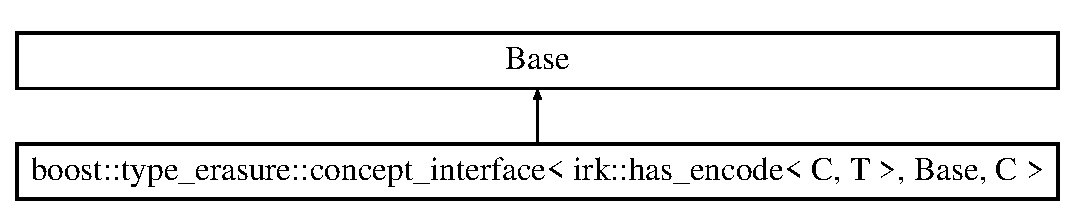
\includegraphics[height=2.000000cm]{structboost_1_1type__erasure_1_1concept__interface_3_01irk_1_1has__encode_3_01C_00_01T_01_4_00_01Base_00_01C_01_4}
\end{center}
\end{figure}
\subsection*{Public Types}
\begin{DoxyCompactItemize}
\item 
using \mbox{\hyperlink{structboost_1_1type__erasure_1_1concept__interface_3_01irk_1_1has__encode_3_01C_00_01T_01_4_00_01Base_00_01C_01_4_a8778ea55db2033d42ecdd9f5e2d24d11}{value\+\_\+type}} = T
\end{DoxyCompactItemize}
\subsection*{Public Member Functions}
\begin{DoxyCompactItemize}
\item 
as\+\_\+param$<$ Base, std\+::ostream \& $>$\+::type \mbox{\hyperlink{structboost_1_1type__erasure_1_1concept__interface_3_01irk_1_1has__encode_3_01C_00_01T_01_4_00_01Base_00_01C_01_4_aaab1ac62febefb2752117b06067e317a}{encode}} (typename as\+\_\+param$<$ Base, T $>$\+::type n, std\+::ostream \&sink) const
\end{DoxyCompactItemize}


\subsection{Member Typedef Documentation}
\mbox{\Hypertarget{structboost_1_1type__erasure_1_1concept__interface_3_01irk_1_1has__encode_3_01C_00_01T_01_4_00_01Base_00_01C_01_4_a8778ea55db2033d42ecdd9f5e2d24d11}\label{structboost_1_1type__erasure_1_1concept__interface_3_01irk_1_1has__encode_3_01C_00_01T_01_4_00_01Base_00_01C_01_4_a8778ea55db2033d42ecdd9f5e2d24d11}} 
\index{boost\+::type\+\_\+erasure\+::concept\+\_\+interface$<$ irk\+::has\+\_\+encode$<$ C, T $>$, Base, C $>$@{boost\+::type\+\_\+erasure\+::concept\+\_\+interface$<$ irk\+::has\+\_\+encode$<$ C, T $>$, Base, C $>$}!value\+\_\+type@{value\+\_\+type}}
\index{value\+\_\+type@{value\+\_\+type}!boost\+::type\+\_\+erasure\+::concept\+\_\+interface$<$ irk\+::has\+\_\+encode$<$ C, T $>$, Base, C $>$@{boost\+::type\+\_\+erasure\+::concept\+\_\+interface$<$ irk\+::has\+\_\+encode$<$ C, T $>$, Base, C $>$}}
\subsubsection{\texorpdfstring{value\+\_\+type}{value\_type}}
{\footnotesize\ttfamily template$<$class C , class T , class Base $>$ \\
using boost\+::type\+\_\+erasure\+::concept\+\_\+interface$<$ \mbox{\hyperlink{structirk_1_1has__encode}{irk\+::has\+\_\+encode}}$<$ C, T $>$, Base, C $>$\+::\mbox{\hyperlink{structboost_1_1type__erasure_1_1concept__interface_3_01irk_1_1has__encode_3_01C_00_01T_01_4_00_01Base_00_01C_01_4_a8778ea55db2033d42ecdd9f5e2d24d11}{value\+\_\+type}} =  T}



\subsection{Member Function Documentation}
\mbox{\Hypertarget{structboost_1_1type__erasure_1_1concept__interface_3_01irk_1_1has__encode_3_01C_00_01T_01_4_00_01Base_00_01C_01_4_aaab1ac62febefb2752117b06067e317a}\label{structboost_1_1type__erasure_1_1concept__interface_3_01irk_1_1has__encode_3_01C_00_01T_01_4_00_01Base_00_01C_01_4_aaab1ac62febefb2752117b06067e317a}} 
\index{boost\+::type\+\_\+erasure\+::concept\+\_\+interface$<$ irk\+::has\+\_\+encode$<$ C, T $>$, Base, C $>$@{boost\+::type\+\_\+erasure\+::concept\+\_\+interface$<$ irk\+::has\+\_\+encode$<$ C, T $>$, Base, C $>$}!encode@{encode}}
\index{encode@{encode}!boost\+::type\+\_\+erasure\+::concept\+\_\+interface$<$ irk\+::has\+\_\+encode$<$ C, T $>$, Base, C $>$@{boost\+::type\+\_\+erasure\+::concept\+\_\+interface$<$ irk\+::has\+\_\+encode$<$ C, T $>$, Base, C $>$}}
\subsubsection{\texorpdfstring{encode()}{encode()}}
{\footnotesize\ttfamily template$<$class C , class T , class Base $>$ \\
as\+\_\+param$<$Base, std\+::ostream\&$>$\+::type boost\+::type\+\_\+erasure\+::concept\+\_\+interface$<$ \mbox{\hyperlink{structirk_1_1has__encode}{irk\+::has\+\_\+encode}}$<$ C, T $>$, Base, C $>$\+::encode (\begin{DoxyParamCaption}\item[{typename as\+\_\+param$<$ Base, T $>$\+::type}]{n,  }\item[{std\+::ostream \&}]{sink }\end{DoxyParamCaption}) const\hspace{0.3cm}{\ttfamily [inline]}}



The documentation for this struct was generated from the following file\+:\begin{DoxyCompactItemize}
\item 
include/irkit/\mbox{\hyperlink{coding_8hpp}{coding.\+hpp}}\end{DoxyCompactItemize}

\hypertarget{structirk_1_1index_1_1skip__list__view_1_1const__iterator}{}\section{irk\+:\+:index\+:\+:skip\+\_\+list\+\_\+view$<$ Skip, element\+\_\+size, Cast\+Fn $>$\+:\+:const\+\_\+iterator Struct Reference}
\label{structirk_1_1index_1_1skip__list__view_1_1const__iterator}\index{irk\+::index\+::skip\+\_\+list\+\_\+view$<$ Skip, element\+\_\+size, Cast\+Fn $>$\+::const\+\_\+iterator@{irk\+::index\+::skip\+\_\+list\+\_\+view$<$ Skip, element\+\_\+size, Cast\+Fn $>$\+::const\+\_\+iterator}}


{\ttfamily \#include $<$skiplist.\+hpp$>$}

\subsection*{Public Types}
\begin{DoxyCompactItemize}
\item 
using \mbox{\hyperlink{structirk_1_1index_1_1skip__list__view_1_1const__iterator_a1b3eae3418d5b4d4f055a6841bd46ffa}{self\+\_\+type}} = \mbox{\hyperlink{structirk_1_1index_1_1skip__list__view_1_1const__iterator}{const\+\_\+iterator}}
\item 
using \mbox{\hyperlink{structirk_1_1index_1_1skip__list__view_1_1const__iterator_a7239886fa2b4671502a6712298b25324}{value\+\_\+type}} = \mbox{\hyperlink{classirk_1_1index_1_1skip__list__view_a7fa2224428803eee24062bb123978755}{skip\+\_\+type}}
\item 
using \mbox{\hyperlink{structirk_1_1index_1_1skip__list__view_1_1const__iterator_ad31e12de91ba22af75cfc00068f80e97}{reference}} = \mbox{\hyperlink{classirk_1_1index_1_1skip__list__view_a7fa2224428803eee24062bb123978755}{skip\+\_\+type}} \&
\item 
using \mbox{\hyperlink{structirk_1_1index_1_1skip__list__view_1_1const__iterator_a1bce3758616ad33105fa64b68a03bd8b}{pointer}} = \mbox{\hyperlink{classirk_1_1index_1_1skip__list__view_a7fa2224428803eee24062bb123978755}{skip\+\_\+type}} $\ast$
\item 
using \mbox{\hyperlink{structirk_1_1index_1_1skip__list__view_1_1const__iterator_aec63e523272f39b50e8420c465440494}{iterator\+\_\+category}} = std\+::bidirectional\+\_\+iterator\+\_\+tag
\item 
using \mbox{\hyperlink{structirk_1_1index_1_1skip__list__view_1_1const__iterator_afcba20bb907a231114679979015f77f5}{difference\+\_\+type}} = std\+::ptrdiff\+\_\+t
\end{DoxyCompactItemize}
\subsection*{Public Member Functions}
\begin{DoxyCompactItemize}
\item 
constexpr \mbox{\hyperlink{classirk_1_1index_1_1skip__list__view_a7fa2224428803eee24062bb123978755}{skip\+\_\+type}} \mbox{\hyperlink{structirk_1_1index_1_1skip__list__view_1_1const__iterator_a986e8294e13ef860e85a3b35640806a2}{operator$\ast$}} () const
\item 
constexpr \mbox{\hyperlink{structirk_1_1index_1_1skip__list__view_1_1const__iterator}{const\+\_\+iterator}} \& \mbox{\hyperlink{structirk_1_1index_1_1skip__list__view_1_1const__iterator_a9f2eff52bff4e4193fa0f89df869a7df}{operator++}} ()
\item 
constexpr \mbox{\hyperlink{structirk_1_1index_1_1skip__list__view_1_1const__iterator}{const\+\_\+iterator}} \mbox{\hyperlink{structirk_1_1index_1_1skip__list__view_1_1const__iterator_a6f847e33643ae607c0c9275edfa69696}{operator++}} (int)
\item 
constexpr \mbox{\hyperlink{structirk_1_1index_1_1skip__list__view_1_1const__iterator}{const\+\_\+iterator}} \& \mbox{\hyperlink{structirk_1_1index_1_1skip__list__view_1_1const__iterator_a08a278c8a621e0a900e44922e05aa013}{operator-\/-\/}} ()
\item 
constexpr \mbox{\hyperlink{structirk_1_1index_1_1skip__list__view_1_1const__iterator}{const\+\_\+iterator}} \mbox{\hyperlink{structirk_1_1index_1_1skip__list__view_1_1const__iterator_a05bfba775a7a9f5036ed8d00f92e67ad}{operator-\/-\/}} (int)
\item 
constexpr \mbox{\hyperlink{structirk_1_1index_1_1skip__list__view_1_1const__iterator}{const\+\_\+iterator}} \mbox{\hyperlink{structirk_1_1index_1_1skip__list__view_1_1const__iterator_aba748a6a37aa356de30370f76d49303b}{operator+}} (\mbox{\hyperlink{structirk_1_1index_1_1skip__list__view_1_1const__iterator_afcba20bb907a231114679979015f77f5}{difference\+\_\+type}} n) const
\item 
constexpr \mbox{\hyperlink{structirk_1_1index_1_1skip__list__view_1_1const__iterator}{const\+\_\+iterator}} \& \mbox{\hyperlink{structirk_1_1index_1_1skip__list__view_1_1const__iterator_a60b3457446cc57d73b0957e193f40674}{operator+=}} (\mbox{\hyperlink{structirk_1_1index_1_1skip__list__view_1_1const__iterator_afcba20bb907a231114679979015f77f5}{difference\+\_\+type}} n)
\item 
constexpr \mbox{\hyperlink{structirk_1_1index_1_1skip__list__view_1_1const__iterator}{const\+\_\+iterator}} \mbox{\hyperlink{structirk_1_1index_1_1skip__list__view_1_1const__iterator_a68650913d3271ded33a0ee4663836ff2}{operator-\/}} (\mbox{\hyperlink{structirk_1_1index_1_1skip__list__view_1_1const__iterator_afcba20bb907a231114679979015f77f5}{difference\+\_\+type}} n) const
\item 
constexpr \mbox{\hyperlink{structirk_1_1index_1_1skip__list__view_1_1const__iterator}{const\+\_\+iterator}} \& \mbox{\hyperlink{structirk_1_1index_1_1skip__list__view_1_1const__iterator_a9c0cdba672b1c2b523ab5a840284d34f}{operator-\/=}} (\mbox{\hyperlink{structirk_1_1index_1_1skip__list__view_1_1const__iterator_afcba20bb907a231114679979015f77f5}{difference\+\_\+type}} n)
\end{DoxyCompactItemize}
\subsection*{Public Attributes}
\begin{DoxyCompactItemize}
\item 
\mbox{\hyperlink{namespaceirk_1_1index_a4089fad8418d09bec3dd2a7ff91d1cea}{byte\+\_\+iterator}} \mbox{\hyperlink{structirk_1_1index_1_1skip__list__view_1_1const__iterator_ae8edc3733ccabb25cbcdc1cdf8b72a9a}{pos}}
\item 
Cast\+Fn \mbox{\hyperlink{structirk_1_1index_1_1skip__list__view_1_1const__iterator_a6e3df1b2579be0c2162535f45a65b000}{cast\+\_\+fn\+\_\+}}
\end{DoxyCompactItemize}
\subsection*{Friends}
\begin{DoxyCompactItemize}
\item 
constexpr friend bool \mbox{\hyperlink{structirk_1_1index_1_1skip__list__view_1_1const__iterator_a665f31dd0863021bd6b740d244346aeb}{operator==}} (\mbox{\hyperlink{structirk_1_1index_1_1skip__list__view_1_1const__iterator}{const\+\_\+iterator}} lhs, \mbox{\hyperlink{structirk_1_1index_1_1skip__list__view_1_1const__iterator}{const\+\_\+iterator}} rhs) noexcept
\item 
constexpr friend bool \mbox{\hyperlink{structirk_1_1index_1_1skip__list__view_1_1const__iterator_a6d10ed131252173e51fcf80bcdabeb72}{operator!=}} (\mbox{\hyperlink{structirk_1_1index_1_1skip__list__view_1_1const__iterator}{const\+\_\+iterator}} lhs, \mbox{\hyperlink{structirk_1_1index_1_1skip__list__view_1_1const__iterator}{const\+\_\+iterator}} rhs) noexcept
\end{DoxyCompactItemize}


\subsection{Member Typedef Documentation}
\mbox{\Hypertarget{structirk_1_1index_1_1skip__list__view_1_1const__iterator_afcba20bb907a231114679979015f77f5}\label{structirk_1_1index_1_1skip__list__view_1_1const__iterator_afcba20bb907a231114679979015f77f5}} 
\index{irk\+::index\+::skip\+\_\+list\+\_\+view\+::const\+\_\+iterator@{irk\+::index\+::skip\+\_\+list\+\_\+view\+::const\+\_\+iterator}!difference\+\_\+type@{difference\+\_\+type}}
\index{difference\+\_\+type@{difference\+\_\+type}!irk\+::index\+::skip\+\_\+list\+\_\+view\+::const\+\_\+iterator@{irk\+::index\+::skip\+\_\+list\+\_\+view\+::const\+\_\+iterator}}
\subsubsection{\texorpdfstring{difference\+\_\+type}{difference\_type}}
{\footnotesize\ttfamily template$<$class Skip , int element\+\_\+size = sizeof(\+Skip), class Cast\+Fn  = irk\+::reinterpret\+\_\+cast\+\_\+fn$<$\+Skip$>$$>$ \\
using \mbox{\hyperlink{classirk_1_1index_1_1skip__list__view}{irk\+::index\+::skip\+\_\+list\+\_\+view}}$<$ Skip, element\+\_\+size, Cast\+Fn $>$\+::\mbox{\hyperlink{structirk_1_1index_1_1skip__list__view_1_1const__iterator_afcba20bb907a231114679979015f77f5}{const\+\_\+iterator\+::difference\+\_\+type}} =  std\+::ptrdiff\+\_\+t}

\mbox{\Hypertarget{structirk_1_1index_1_1skip__list__view_1_1const__iterator_aec63e523272f39b50e8420c465440494}\label{structirk_1_1index_1_1skip__list__view_1_1const__iterator_aec63e523272f39b50e8420c465440494}} 
\index{irk\+::index\+::skip\+\_\+list\+\_\+view\+::const\+\_\+iterator@{irk\+::index\+::skip\+\_\+list\+\_\+view\+::const\+\_\+iterator}!iterator\+\_\+category@{iterator\+\_\+category}}
\index{iterator\+\_\+category@{iterator\+\_\+category}!irk\+::index\+::skip\+\_\+list\+\_\+view\+::const\+\_\+iterator@{irk\+::index\+::skip\+\_\+list\+\_\+view\+::const\+\_\+iterator}}
\subsubsection{\texorpdfstring{iterator\+\_\+category}{iterator\_category}}
{\footnotesize\ttfamily template$<$class Skip , int element\+\_\+size = sizeof(\+Skip), class Cast\+Fn  = irk\+::reinterpret\+\_\+cast\+\_\+fn$<$\+Skip$>$$>$ \\
using \mbox{\hyperlink{classirk_1_1index_1_1skip__list__view}{irk\+::index\+::skip\+\_\+list\+\_\+view}}$<$ Skip, element\+\_\+size, Cast\+Fn $>$\+::\mbox{\hyperlink{structirk_1_1index_1_1skip__list__view_1_1const__iterator_aec63e523272f39b50e8420c465440494}{const\+\_\+iterator\+::iterator\+\_\+category}} =  std\+::bidirectional\+\_\+iterator\+\_\+tag}

\mbox{\Hypertarget{structirk_1_1index_1_1skip__list__view_1_1const__iterator_a1bce3758616ad33105fa64b68a03bd8b}\label{structirk_1_1index_1_1skip__list__view_1_1const__iterator_a1bce3758616ad33105fa64b68a03bd8b}} 
\index{irk\+::index\+::skip\+\_\+list\+\_\+view\+::const\+\_\+iterator@{irk\+::index\+::skip\+\_\+list\+\_\+view\+::const\+\_\+iterator}!pointer@{pointer}}
\index{pointer@{pointer}!irk\+::index\+::skip\+\_\+list\+\_\+view\+::const\+\_\+iterator@{irk\+::index\+::skip\+\_\+list\+\_\+view\+::const\+\_\+iterator}}
\subsubsection{\texorpdfstring{pointer}{pointer}}
{\footnotesize\ttfamily template$<$class Skip , int element\+\_\+size = sizeof(\+Skip), class Cast\+Fn  = irk\+::reinterpret\+\_\+cast\+\_\+fn$<$\+Skip$>$$>$ \\
using \mbox{\hyperlink{classirk_1_1index_1_1skip__list__view}{irk\+::index\+::skip\+\_\+list\+\_\+view}}$<$ Skip, element\+\_\+size, Cast\+Fn $>$\+::\mbox{\hyperlink{structirk_1_1index_1_1skip__list__view_1_1const__iterator_a1bce3758616ad33105fa64b68a03bd8b}{const\+\_\+iterator\+::pointer}} =  \mbox{\hyperlink{classirk_1_1index_1_1skip__list__view_a7fa2224428803eee24062bb123978755}{skip\+\_\+type}}$\ast$}

\mbox{\Hypertarget{structirk_1_1index_1_1skip__list__view_1_1const__iterator_ad31e12de91ba22af75cfc00068f80e97}\label{structirk_1_1index_1_1skip__list__view_1_1const__iterator_ad31e12de91ba22af75cfc00068f80e97}} 
\index{irk\+::index\+::skip\+\_\+list\+\_\+view\+::const\+\_\+iterator@{irk\+::index\+::skip\+\_\+list\+\_\+view\+::const\+\_\+iterator}!reference@{reference}}
\index{reference@{reference}!irk\+::index\+::skip\+\_\+list\+\_\+view\+::const\+\_\+iterator@{irk\+::index\+::skip\+\_\+list\+\_\+view\+::const\+\_\+iterator}}
\subsubsection{\texorpdfstring{reference}{reference}}
{\footnotesize\ttfamily template$<$class Skip , int element\+\_\+size = sizeof(\+Skip), class Cast\+Fn  = irk\+::reinterpret\+\_\+cast\+\_\+fn$<$\+Skip$>$$>$ \\
using \mbox{\hyperlink{classirk_1_1index_1_1skip__list__view}{irk\+::index\+::skip\+\_\+list\+\_\+view}}$<$ Skip, element\+\_\+size, Cast\+Fn $>$\+::\mbox{\hyperlink{structirk_1_1index_1_1skip__list__view_1_1const__iterator_ad31e12de91ba22af75cfc00068f80e97}{const\+\_\+iterator\+::reference}} =  \mbox{\hyperlink{classirk_1_1index_1_1skip__list__view_a7fa2224428803eee24062bb123978755}{skip\+\_\+type}}\&}

\mbox{\Hypertarget{structirk_1_1index_1_1skip__list__view_1_1const__iterator_a1b3eae3418d5b4d4f055a6841bd46ffa}\label{structirk_1_1index_1_1skip__list__view_1_1const__iterator_a1b3eae3418d5b4d4f055a6841bd46ffa}} 
\index{irk\+::index\+::skip\+\_\+list\+\_\+view\+::const\+\_\+iterator@{irk\+::index\+::skip\+\_\+list\+\_\+view\+::const\+\_\+iterator}!self\+\_\+type@{self\+\_\+type}}
\index{self\+\_\+type@{self\+\_\+type}!irk\+::index\+::skip\+\_\+list\+\_\+view\+::const\+\_\+iterator@{irk\+::index\+::skip\+\_\+list\+\_\+view\+::const\+\_\+iterator}}
\subsubsection{\texorpdfstring{self\+\_\+type}{self\_type}}
{\footnotesize\ttfamily template$<$class Skip , int element\+\_\+size = sizeof(\+Skip), class Cast\+Fn  = irk\+::reinterpret\+\_\+cast\+\_\+fn$<$\+Skip$>$$>$ \\
using \mbox{\hyperlink{classirk_1_1index_1_1skip__list__view}{irk\+::index\+::skip\+\_\+list\+\_\+view}}$<$ Skip, element\+\_\+size, Cast\+Fn $>$\+::\mbox{\hyperlink{structirk_1_1index_1_1skip__list__view_1_1const__iterator_a1b3eae3418d5b4d4f055a6841bd46ffa}{const\+\_\+iterator\+::self\+\_\+type}} =  \mbox{\hyperlink{structirk_1_1index_1_1skip__list__view_1_1const__iterator}{const\+\_\+iterator}}}

\mbox{\Hypertarget{structirk_1_1index_1_1skip__list__view_1_1const__iterator_a7239886fa2b4671502a6712298b25324}\label{structirk_1_1index_1_1skip__list__view_1_1const__iterator_a7239886fa2b4671502a6712298b25324}} 
\index{irk\+::index\+::skip\+\_\+list\+\_\+view\+::const\+\_\+iterator@{irk\+::index\+::skip\+\_\+list\+\_\+view\+::const\+\_\+iterator}!value\+\_\+type@{value\+\_\+type}}
\index{value\+\_\+type@{value\+\_\+type}!irk\+::index\+::skip\+\_\+list\+\_\+view\+::const\+\_\+iterator@{irk\+::index\+::skip\+\_\+list\+\_\+view\+::const\+\_\+iterator}}
\subsubsection{\texorpdfstring{value\+\_\+type}{value\_type}}
{\footnotesize\ttfamily template$<$class Skip , int element\+\_\+size = sizeof(\+Skip), class Cast\+Fn  = irk\+::reinterpret\+\_\+cast\+\_\+fn$<$\+Skip$>$$>$ \\
using \mbox{\hyperlink{classirk_1_1index_1_1skip__list__view}{irk\+::index\+::skip\+\_\+list\+\_\+view}}$<$ Skip, element\+\_\+size, Cast\+Fn $>$\+::\mbox{\hyperlink{structirk_1_1index_1_1skip__list__view_1_1const__iterator_a7239886fa2b4671502a6712298b25324}{const\+\_\+iterator\+::value\+\_\+type}} =  \mbox{\hyperlink{classirk_1_1index_1_1skip__list__view_a7fa2224428803eee24062bb123978755}{skip\+\_\+type}}}



\subsection{Member Function Documentation}
\mbox{\Hypertarget{structirk_1_1index_1_1skip__list__view_1_1const__iterator_a986e8294e13ef860e85a3b35640806a2}\label{structirk_1_1index_1_1skip__list__view_1_1const__iterator_a986e8294e13ef860e85a3b35640806a2}} 
\index{irk\+::index\+::skip\+\_\+list\+\_\+view\+::const\+\_\+iterator@{irk\+::index\+::skip\+\_\+list\+\_\+view\+::const\+\_\+iterator}!operator$\ast$@{operator$\ast$}}
\index{operator$\ast$@{operator$\ast$}!irk\+::index\+::skip\+\_\+list\+\_\+view\+::const\+\_\+iterator@{irk\+::index\+::skip\+\_\+list\+\_\+view\+::const\+\_\+iterator}}
\subsubsection{\texorpdfstring{operator$\ast$()}{operator*()}}
{\footnotesize\ttfamily template$<$class Skip , int element\+\_\+size = sizeof(\+Skip), class Cast\+Fn  = irk\+::reinterpret\+\_\+cast\+\_\+fn$<$\+Skip$>$$>$ \\
constexpr \mbox{\hyperlink{classirk_1_1index_1_1skip__list__view_a7fa2224428803eee24062bb123978755}{skip\+\_\+type}} \mbox{\hyperlink{classirk_1_1index_1_1skip__list__view}{irk\+::index\+::skip\+\_\+list\+\_\+view}}$<$ Skip, element\+\_\+size, Cast\+Fn $>$\+::const\+\_\+iterator\+::operator$\ast$ (\begin{DoxyParamCaption}{ }\end{DoxyParamCaption}) const\hspace{0.3cm}{\ttfamily [inline]}}

\mbox{\Hypertarget{structirk_1_1index_1_1skip__list__view_1_1const__iterator_aba748a6a37aa356de30370f76d49303b}\label{structirk_1_1index_1_1skip__list__view_1_1const__iterator_aba748a6a37aa356de30370f76d49303b}} 
\index{irk\+::index\+::skip\+\_\+list\+\_\+view\+::const\+\_\+iterator@{irk\+::index\+::skip\+\_\+list\+\_\+view\+::const\+\_\+iterator}!operator+@{operator+}}
\index{operator+@{operator+}!irk\+::index\+::skip\+\_\+list\+\_\+view\+::const\+\_\+iterator@{irk\+::index\+::skip\+\_\+list\+\_\+view\+::const\+\_\+iterator}}
\subsubsection{\texorpdfstring{operator+()}{operator+()}}
{\footnotesize\ttfamily template$<$class Skip , int element\+\_\+size = sizeof(\+Skip), class Cast\+Fn  = irk\+::reinterpret\+\_\+cast\+\_\+fn$<$\+Skip$>$$>$ \\
constexpr \mbox{\hyperlink{structirk_1_1index_1_1skip__list__view_1_1const__iterator}{const\+\_\+iterator}} \mbox{\hyperlink{classirk_1_1index_1_1skip__list__view}{irk\+::index\+::skip\+\_\+list\+\_\+view}}$<$ Skip, element\+\_\+size, Cast\+Fn $>$\+::const\+\_\+iterator\+::operator+ (\begin{DoxyParamCaption}\item[{\mbox{\hyperlink{structirk_1_1index_1_1skip__list__view_1_1const__iterator_afcba20bb907a231114679979015f77f5}{difference\+\_\+type}}}]{n }\end{DoxyParamCaption}) const\hspace{0.3cm}{\ttfamily [inline]}}

\mbox{\Hypertarget{structirk_1_1index_1_1skip__list__view_1_1const__iterator_a9f2eff52bff4e4193fa0f89df869a7df}\label{structirk_1_1index_1_1skip__list__view_1_1const__iterator_a9f2eff52bff4e4193fa0f89df869a7df}} 
\index{irk\+::index\+::skip\+\_\+list\+\_\+view\+::const\+\_\+iterator@{irk\+::index\+::skip\+\_\+list\+\_\+view\+::const\+\_\+iterator}!operator++@{operator++}}
\index{operator++@{operator++}!irk\+::index\+::skip\+\_\+list\+\_\+view\+::const\+\_\+iterator@{irk\+::index\+::skip\+\_\+list\+\_\+view\+::const\+\_\+iterator}}
\subsubsection{\texorpdfstring{operator++()}{operator++()}\hspace{0.1cm}{\footnotesize\ttfamily [1/2]}}
{\footnotesize\ttfamily template$<$class Skip , int element\+\_\+size = sizeof(\+Skip), class Cast\+Fn  = irk\+::reinterpret\+\_\+cast\+\_\+fn$<$\+Skip$>$$>$ \\
constexpr \mbox{\hyperlink{structirk_1_1index_1_1skip__list__view_1_1const__iterator}{const\+\_\+iterator}}\& \mbox{\hyperlink{classirk_1_1index_1_1skip__list__view}{irk\+::index\+::skip\+\_\+list\+\_\+view}}$<$ Skip, element\+\_\+size, Cast\+Fn $>$\+::const\+\_\+iterator\+::operator++ (\begin{DoxyParamCaption}{ }\end{DoxyParamCaption})\hspace{0.3cm}{\ttfamily [inline]}}

\mbox{\Hypertarget{structirk_1_1index_1_1skip__list__view_1_1const__iterator_a6f847e33643ae607c0c9275edfa69696}\label{structirk_1_1index_1_1skip__list__view_1_1const__iterator_a6f847e33643ae607c0c9275edfa69696}} 
\index{irk\+::index\+::skip\+\_\+list\+\_\+view\+::const\+\_\+iterator@{irk\+::index\+::skip\+\_\+list\+\_\+view\+::const\+\_\+iterator}!operator++@{operator++}}
\index{operator++@{operator++}!irk\+::index\+::skip\+\_\+list\+\_\+view\+::const\+\_\+iterator@{irk\+::index\+::skip\+\_\+list\+\_\+view\+::const\+\_\+iterator}}
\subsubsection{\texorpdfstring{operator++()}{operator++()}\hspace{0.1cm}{\footnotesize\ttfamily [2/2]}}
{\footnotesize\ttfamily template$<$class Skip , int element\+\_\+size = sizeof(\+Skip), class Cast\+Fn  = irk\+::reinterpret\+\_\+cast\+\_\+fn$<$\+Skip$>$$>$ \\
constexpr \mbox{\hyperlink{structirk_1_1index_1_1skip__list__view_1_1const__iterator}{const\+\_\+iterator}} \mbox{\hyperlink{classirk_1_1index_1_1skip__list__view}{irk\+::index\+::skip\+\_\+list\+\_\+view}}$<$ Skip, element\+\_\+size, Cast\+Fn $>$\+::const\+\_\+iterator\+::operator++ (\begin{DoxyParamCaption}\item[{int}]{ }\end{DoxyParamCaption})\hspace{0.3cm}{\ttfamily [inline]}}

\mbox{\Hypertarget{structirk_1_1index_1_1skip__list__view_1_1const__iterator_a60b3457446cc57d73b0957e193f40674}\label{structirk_1_1index_1_1skip__list__view_1_1const__iterator_a60b3457446cc57d73b0957e193f40674}} 
\index{irk\+::index\+::skip\+\_\+list\+\_\+view\+::const\+\_\+iterator@{irk\+::index\+::skip\+\_\+list\+\_\+view\+::const\+\_\+iterator}!operator+=@{operator+=}}
\index{operator+=@{operator+=}!irk\+::index\+::skip\+\_\+list\+\_\+view\+::const\+\_\+iterator@{irk\+::index\+::skip\+\_\+list\+\_\+view\+::const\+\_\+iterator}}
\subsubsection{\texorpdfstring{operator+=()}{operator+=()}}
{\footnotesize\ttfamily template$<$class Skip , int element\+\_\+size = sizeof(\+Skip), class Cast\+Fn  = irk\+::reinterpret\+\_\+cast\+\_\+fn$<$\+Skip$>$$>$ \\
constexpr \mbox{\hyperlink{structirk_1_1index_1_1skip__list__view_1_1const__iterator}{const\+\_\+iterator}}\& \mbox{\hyperlink{classirk_1_1index_1_1skip__list__view}{irk\+::index\+::skip\+\_\+list\+\_\+view}}$<$ Skip, element\+\_\+size, Cast\+Fn $>$\+::const\+\_\+iterator\+::operator+= (\begin{DoxyParamCaption}\item[{\mbox{\hyperlink{structirk_1_1index_1_1skip__list__view_1_1const__iterator_afcba20bb907a231114679979015f77f5}{difference\+\_\+type}}}]{n }\end{DoxyParamCaption})\hspace{0.3cm}{\ttfamily [inline]}}

\mbox{\Hypertarget{structirk_1_1index_1_1skip__list__view_1_1const__iterator_a68650913d3271ded33a0ee4663836ff2}\label{structirk_1_1index_1_1skip__list__view_1_1const__iterator_a68650913d3271ded33a0ee4663836ff2}} 
\index{irk\+::index\+::skip\+\_\+list\+\_\+view\+::const\+\_\+iterator@{irk\+::index\+::skip\+\_\+list\+\_\+view\+::const\+\_\+iterator}!operator-\/@{operator-\/}}
\index{operator-\/@{operator-\/}!irk\+::index\+::skip\+\_\+list\+\_\+view\+::const\+\_\+iterator@{irk\+::index\+::skip\+\_\+list\+\_\+view\+::const\+\_\+iterator}}
\subsubsection{\texorpdfstring{operator-\/()}{operator-()}}
{\footnotesize\ttfamily template$<$class Skip , int element\+\_\+size = sizeof(\+Skip), class Cast\+Fn  = irk\+::reinterpret\+\_\+cast\+\_\+fn$<$\+Skip$>$$>$ \\
constexpr \mbox{\hyperlink{structirk_1_1index_1_1skip__list__view_1_1const__iterator}{const\+\_\+iterator}} \mbox{\hyperlink{classirk_1_1index_1_1skip__list__view}{irk\+::index\+::skip\+\_\+list\+\_\+view}}$<$ Skip, element\+\_\+size, Cast\+Fn $>$\+::const\+\_\+iterator\+::operator-\/ (\begin{DoxyParamCaption}\item[{\mbox{\hyperlink{structirk_1_1index_1_1skip__list__view_1_1const__iterator_afcba20bb907a231114679979015f77f5}{difference\+\_\+type}}}]{n }\end{DoxyParamCaption}) const\hspace{0.3cm}{\ttfamily [inline]}}

\mbox{\Hypertarget{structirk_1_1index_1_1skip__list__view_1_1const__iterator_a08a278c8a621e0a900e44922e05aa013}\label{structirk_1_1index_1_1skip__list__view_1_1const__iterator_a08a278c8a621e0a900e44922e05aa013}} 
\index{irk\+::index\+::skip\+\_\+list\+\_\+view\+::const\+\_\+iterator@{irk\+::index\+::skip\+\_\+list\+\_\+view\+::const\+\_\+iterator}!operator-\/-\/@{operator-\/-\/}}
\index{operator-\/-\/@{operator-\/-\/}!irk\+::index\+::skip\+\_\+list\+\_\+view\+::const\+\_\+iterator@{irk\+::index\+::skip\+\_\+list\+\_\+view\+::const\+\_\+iterator}}
\subsubsection{\texorpdfstring{operator-\/-\/()}{operator--()}\hspace{0.1cm}{\footnotesize\ttfamily [1/2]}}
{\footnotesize\ttfamily template$<$class Skip , int element\+\_\+size = sizeof(\+Skip), class Cast\+Fn  = irk\+::reinterpret\+\_\+cast\+\_\+fn$<$\+Skip$>$$>$ \\
constexpr \mbox{\hyperlink{structirk_1_1index_1_1skip__list__view_1_1const__iterator}{const\+\_\+iterator}}\& \mbox{\hyperlink{classirk_1_1index_1_1skip__list__view}{irk\+::index\+::skip\+\_\+list\+\_\+view}}$<$ Skip, element\+\_\+size, Cast\+Fn $>$\+::const\+\_\+iterator\+::operator-\/-\/ (\begin{DoxyParamCaption}{ }\end{DoxyParamCaption})\hspace{0.3cm}{\ttfamily [inline]}}

\mbox{\Hypertarget{structirk_1_1index_1_1skip__list__view_1_1const__iterator_a05bfba775a7a9f5036ed8d00f92e67ad}\label{structirk_1_1index_1_1skip__list__view_1_1const__iterator_a05bfba775a7a9f5036ed8d00f92e67ad}} 
\index{irk\+::index\+::skip\+\_\+list\+\_\+view\+::const\+\_\+iterator@{irk\+::index\+::skip\+\_\+list\+\_\+view\+::const\+\_\+iterator}!operator-\/-\/@{operator-\/-\/}}
\index{operator-\/-\/@{operator-\/-\/}!irk\+::index\+::skip\+\_\+list\+\_\+view\+::const\+\_\+iterator@{irk\+::index\+::skip\+\_\+list\+\_\+view\+::const\+\_\+iterator}}
\subsubsection{\texorpdfstring{operator-\/-\/()}{operator--()}\hspace{0.1cm}{\footnotesize\ttfamily [2/2]}}
{\footnotesize\ttfamily template$<$class Skip , int element\+\_\+size = sizeof(\+Skip), class Cast\+Fn  = irk\+::reinterpret\+\_\+cast\+\_\+fn$<$\+Skip$>$$>$ \\
constexpr \mbox{\hyperlink{structirk_1_1index_1_1skip__list__view_1_1const__iterator}{const\+\_\+iterator}} \mbox{\hyperlink{classirk_1_1index_1_1skip__list__view}{irk\+::index\+::skip\+\_\+list\+\_\+view}}$<$ Skip, element\+\_\+size, Cast\+Fn $>$\+::const\+\_\+iterator\+::operator-\/-\/ (\begin{DoxyParamCaption}\item[{int}]{ }\end{DoxyParamCaption})\hspace{0.3cm}{\ttfamily [inline]}}

\mbox{\Hypertarget{structirk_1_1index_1_1skip__list__view_1_1const__iterator_a9c0cdba672b1c2b523ab5a840284d34f}\label{structirk_1_1index_1_1skip__list__view_1_1const__iterator_a9c0cdba672b1c2b523ab5a840284d34f}} 
\index{irk\+::index\+::skip\+\_\+list\+\_\+view\+::const\+\_\+iterator@{irk\+::index\+::skip\+\_\+list\+\_\+view\+::const\+\_\+iterator}!operator-\/=@{operator-\/=}}
\index{operator-\/=@{operator-\/=}!irk\+::index\+::skip\+\_\+list\+\_\+view\+::const\+\_\+iterator@{irk\+::index\+::skip\+\_\+list\+\_\+view\+::const\+\_\+iterator}}
\subsubsection{\texorpdfstring{operator-\/=()}{operator-=()}}
{\footnotesize\ttfamily template$<$class Skip , int element\+\_\+size = sizeof(\+Skip), class Cast\+Fn  = irk\+::reinterpret\+\_\+cast\+\_\+fn$<$\+Skip$>$$>$ \\
constexpr \mbox{\hyperlink{structirk_1_1index_1_1skip__list__view_1_1const__iterator}{const\+\_\+iterator}}\& \mbox{\hyperlink{classirk_1_1index_1_1skip__list__view}{irk\+::index\+::skip\+\_\+list\+\_\+view}}$<$ Skip, element\+\_\+size, Cast\+Fn $>$\+::const\+\_\+iterator\+::operator-\/= (\begin{DoxyParamCaption}\item[{\mbox{\hyperlink{structirk_1_1index_1_1skip__list__view_1_1const__iterator_afcba20bb907a231114679979015f77f5}{difference\+\_\+type}}}]{n }\end{DoxyParamCaption})\hspace{0.3cm}{\ttfamily [inline]}}



\subsection{Friends And Related Function Documentation}
\mbox{\Hypertarget{structirk_1_1index_1_1skip__list__view_1_1const__iterator_a6d10ed131252173e51fcf80bcdabeb72}\label{structirk_1_1index_1_1skip__list__view_1_1const__iterator_a6d10ed131252173e51fcf80bcdabeb72}} 
\index{irk\+::index\+::skip\+\_\+list\+\_\+view\+::const\+\_\+iterator@{irk\+::index\+::skip\+\_\+list\+\_\+view\+::const\+\_\+iterator}!operator"!=@{operator"!=}}
\index{operator"!=@{operator"!=}!irk\+::index\+::skip\+\_\+list\+\_\+view\+::const\+\_\+iterator@{irk\+::index\+::skip\+\_\+list\+\_\+view\+::const\+\_\+iterator}}
\subsubsection{\texorpdfstring{operator"!=}{operator!=}}
{\footnotesize\ttfamily template$<$class Skip , int element\+\_\+size = sizeof(\+Skip), class Cast\+Fn  = irk\+::reinterpret\+\_\+cast\+\_\+fn$<$\+Skip$>$$>$ \\
constexpr friend bool operator!= (\begin{DoxyParamCaption}\item[{\mbox{\hyperlink{structirk_1_1index_1_1skip__list__view_1_1const__iterator}{const\+\_\+iterator}}}]{lhs,  }\item[{\mbox{\hyperlink{structirk_1_1index_1_1skip__list__view_1_1const__iterator}{const\+\_\+iterator}}}]{rhs }\end{DoxyParamCaption})\hspace{0.3cm}{\ttfamily [friend]}}

\mbox{\Hypertarget{structirk_1_1index_1_1skip__list__view_1_1const__iterator_a665f31dd0863021bd6b740d244346aeb}\label{structirk_1_1index_1_1skip__list__view_1_1const__iterator_a665f31dd0863021bd6b740d244346aeb}} 
\index{irk\+::index\+::skip\+\_\+list\+\_\+view\+::const\+\_\+iterator@{irk\+::index\+::skip\+\_\+list\+\_\+view\+::const\+\_\+iterator}!operator==@{operator==}}
\index{operator==@{operator==}!irk\+::index\+::skip\+\_\+list\+\_\+view\+::const\+\_\+iterator@{irk\+::index\+::skip\+\_\+list\+\_\+view\+::const\+\_\+iterator}}
\subsubsection{\texorpdfstring{operator==}{operator==}}
{\footnotesize\ttfamily template$<$class Skip , int element\+\_\+size = sizeof(\+Skip), class Cast\+Fn  = irk\+::reinterpret\+\_\+cast\+\_\+fn$<$\+Skip$>$$>$ \\
constexpr friend bool operator== (\begin{DoxyParamCaption}\item[{\mbox{\hyperlink{structirk_1_1index_1_1skip__list__view_1_1const__iterator}{const\+\_\+iterator}}}]{lhs,  }\item[{\mbox{\hyperlink{structirk_1_1index_1_1skip__list__view_1_1const__iterator}{const\+\_\+iterator}}}]{rhs }\end{DoxyParamCaption})\hspace{0.3cm}{\ttfamily [friend]}}



\subsection{Member Data Documentation}
\mbox{\Hypertarget{structirk_1_1index_1_1skip__list__view_1_1const__iterator_a6e3df1b2579be0c2162535f45a65b000}\label{structirk_1_1index_1_1skip__list__view_1_1const__iterator_a6e3df1b2579be0c2162535f45a65b000}} 
\index{irk\+::index\+::skip\+\_\+list\+\_\+view\+::const\+\_\+iterator@{irk\+::index\+::skip\+\_\+list\+\_\+view\+::const\+\_\+iterator}!cast\+\_\+fn\+\_\+@{cast\+\_\+fn\+\_\+}}
\index{cast\+\_\+fn\+\_\+@{cast\+\_\+fn\+\_\+}!irk\+::index\+::skip\+\_\+list\+\_\+view\+::const\+\_\+iterator@{irk\+::index\+::skip\+\_\+list\+\_\+view\+::const\+\_\+iterator}}
\subsubsection{\texorpdfstring{cast\+\_\+fn\+\_\+}{cast\_fn\_}}
{\footnotesize\ttfamily template$<$class Skip , int element\+\_\+size = sizeof(\+Skip), class Cast\+Fn  = irk\+::reinterpret\+\_\+cast\+\_\+fn$<$\+Skip$>$$>$ \\
Cast\+Fn \mbox{\hyperlink{classirk_1_1index_1_1skip__list__view}{irk\+::index\+::skip\+\_\+list\+\_\+view}}$<$ Skip, element\+\_\+size, Cast\+Fn $>$\+::const\+\_\+iterator\+::cast\+\_\+fn\+\_\+}

\mbox{\Hypertarget{structirk_1_1index_1_1skip__list__view_1_1const__iterator_ae8edc3733ccabb25cbcdc1cdf8b72a9a}\label{structirk_1_1index_1_1skip__list__view_1_1const__iterator_ae8edc3733ccabb25cbcdc1cdf8b72a9a}} 
\index{irk\+::index\+::skip\+\_\+list\+\_\+view\+::const\+\_\+iterator@{irk\+::index\+::skip\+\_\+list\+\_\+view\+::const\+\_\+iterator}!pos@{pos}}
\index{pos@{pos}!irk\+::index\+::skip\+\_\+list\+\_\+view\+::const\+\_\+iterator@{irk\+::index\+::skip\+\_\+list\+\_\+view\+::const\+\_\+iterator}}
\subsubsection{\texorpdfstring{pos}{pos}}
{\footnotesize\ttfamily template$<$class Skip , int element\+\_\+size = sizeof(\+Skip), class Cast\+Fn  = irk\+::reinterpret\+\_\+cast\+\_\+fn$<$\+Skip$>$$>$ \\
\mbox{\hyperlink{namespaceirk_1_1index_a4089fad8418d09bec3dd2a7ff91d1cea}{byte\+\_\+iterator}} \mbox{\hyperlink{classirk_1_1index_1_1skip__list__view}{irk\+::index\+::skip\+\_\+list\+\_\+view}}$<$ Skip, element\+\_\+size, Cast\+Fn $>$\+::const\+\_\+iterator\+::pos}



The documentation for this struct was generated from the following file\+:\begin{DoxyCompactItemize}
\item 
include/irkit/index/\mbox{\hyperlink{skiplist_8hpp}{skiplist.\+hpp}}\end{DoxyCompactItemize}

\hypertarget{classirk_1_1view_1_1ZipView_1_1const__iterator}{}\section{irk\+:\+:view\+:\+:Zip\+View$<$ Zip\+Fn, Left\+Range, Right\+Range $>$\+:\+:const\+\_\+iterator Class Reference}
\label{classirk_1_1view_1_1ZipView_1_1const__iterator}\index{irk\+::view\+::\+Zip\+View$<$ Zip\+Fn, Left\+Range, Right\+Range $>$\+::const\+\_\+iterator@{irk\+::view\+::\+Zip\+View$<$ Zip\+Fn, Left\+Range, Right\+Range $>$\+::const\+\_\+iterator}}


{\ttfamily \#include $<$utils.\+hpp$>$}

\subsection*{Public Member Functions}
\begin{DoxyCompactItemize}
\item 
\mbox{\hyperlink{classirk_1_1view_1_1ZipView_1_1const__iterator_a609776c989ec542de0baf29c2c413b6d}{const\+\_\+iterator}} (\mbox{\hyperlink{namespaceirk_a90f7893fdbf95c6dcc2302148eb0bddb}{const\+\_\+iterator\+\_\+t}}$<$ Left\+Range $>$ liter, \mbox{\hyperlink{namespaceirk_a90f7893fdbf95c6dcc2302148eb0bddb}{const\+\_\+iterator\+\_\+t}}$<$ Right\+Range $>$ riter, Zip\+Fn zip\+\_\+fn)
\item 
bool \mbox{\hyperlink{classirk_1_1view_1_1ZipView_1_1const__iterator_a1ae00d4c143e3a594c228aedc41b322a}{operator==}} (const \mbox{\hyperlink{classirk_1_1view_1_1ZipView_1_1const__iterator}{const\+\_\+iterator}} \&rhs) const
\item 
bool \mbox{\hyperlink{classirk_1_1view_1_1ZipView_1_1const__iterator_acfba3a3b55f15c9485ae1f84d900d579}{operator!=}} (const \mbox{\hyperlink{classirk_1_1view_1_1ZipView_1_1const__iterator}{const\+\_\+iterator}} \&rhs) const
\item 
void \mbox{\hyperlink{classirk_1_1view_1_1ZipView_1_1const__iterator_a924c85dc6681afea47f98bcbf2f49c47}{operator++}} ()
\item 
void \mbox{\hyperlink{classirk_1_1view_1_1ZipView_1_1const__iterator_a7242e63b9c852a5f9947876965930a56}{operator++}} (int)
\item 
auto \mbox{\hyperlink{classirk_1_1view_1_1ZipView_1_1const__iterator_ac95ceb30ed54868d908b786008b60610}{operator$\ast$}} ()
\end{DoxyCompactItemize}


\subsection{Constructor \& Destructor Documentation}
\mbox{\Hypertarget{classirk_1_1view_1_1ZipView_1_1const__iterator_a609776c989ec542de0baf29c2c413b6d}\label{classirk_1_1view_1_1ZipView_1_1const__iterator_a609776c989ec542de0baf29c2c413b6d}} 
\index{irk\+::view\+::\+Zip\+View\+::const\+\_\+iterator@{irk\+::view\+::\+Zip\+View\+::const\+\_\+iterator}!const\+\_\+iterator@{const\+\_\+iterator}}
\index{const\+\_\+iterator@{const\+\_\+iterator}!irk\+::view\+::\+Zip\+View\+::const\+\_\+iterator@{irk\+::view\+::\+Zip\+View\+::const\+\_\+iterator}}
\subsubsection{\texorpdfstring{const\+\_\+iterator()}{const\_iterator()}}
{\footnotesize\ttfamily template$<$class Zip\+Fn , class Left\+Range , class Right\+Range $>$ \\
\mbox{\hyperlink{classirk_1_1view_1_1ZipView}{irk\+::view\+::\+Zip\+View}}$<$ Zip\+Fn, Left\+Range, Right\+Range $>$\+::const\+\_\+iterator\+::const\+\_\+iterator (\begin{DoxyParamCaption}\item[{\mbox{\hyperlink{namespaceirk_a90f7893fdbf95c6dcc2302148eb0bddb}{const\+\_\+iterator\+\_\+t}}$<$ Left\+Range $>$}]{liter,  }\item[{\mbox{\hyperlink{namespaceirk_a90f7893fdbf95c6dcc2302148eb0bddb}{const\+\_\+iterator\+\_\+t}}$<$ Right\+Range $>$}]{riter,  }\item[{Zip\+Fn}]{zip\+\_\+fn }\end{DoxyParamCaption})\hspace{0.3cm}{\ttfamily [inline]}}



\subsection{Member Function Documentation}
\mbox{\Hypertarget{classirk_1_1view_1_1ZipView_1_1const__iterator_acfba3a3b55f15c9485ae1f84d900d579}\label{classirk_1_1view_1_1ZipView_1_1const__iterator_acfba3a3b55f15c9485ae1f84d900d579}} 
\index{irk\+::view\+::\+Zip\+View\+::const\+\_\+iterator@{irk\+::view\+::\+Zip\+View\+::const\+\_\+iterator}!operator"!=@{operator"!=}}
\index{operator"!=@{operator"!=}!irk\+::view\+::\+Zip\+View\+::const\+\_\+iterator@{irk\+::view\+::\+Zip\+View\+::const\+\_\+iterator}}
\subsubsection{\texorpdfstring{operator"!=()}{operator!=()}}
{\footnotesize\ttfamily template$<$class Zip\+Fn , class Left\+Range , class Right\+Range $>$ \\
bool \mbox{\hyperlink{classirk_1_1view_1_1ZipView}{irk\+::view\+::\+Zip\+View}}$<$ Zip\+Fn, Left\+Range, Right\+Range $>$\+::const\+\_\+iterator\+::operator!= (\begin{DoxyParamCaption}\item[{const \mbox{\hyperlink{classirk_1_1view_1_1ZipView_1_1const__iterator}{const\+\_\+iterator}} \&}]{rhs }\end{DoxyParamCaption}) const\hspace{0.3cm}{\ttfamily [inline]}}

\mbox{\Hypertarget{classirk_1_1view_1_1ZipView_1_1const__iterator_ac95ceb30ed54868d908b786008b60610}\label{classirk_1_1view_1_1ZipView_1_1const__iterator_ac95ceb30ed54868d908b786008b60610}} 
\index{irk\+::view\+::\+Zip\+View\+::const\+\_\+iterator@{irk\+::view\+::\+Zip\+View\+::const\+\_\+iterator}!operator$\ast$@{operator$\ast$}}
\index{operator$\ast$@{operator$\ast$}!irk\+::view\+::\+Zip\+View\+::const\+\_\+iterator@{irk\+::view\+::\+Zip\+View\+::const\+\_\+iterator}}
\subsubsection{\texorpdfstring{operator$\ast$()}{operator*()}}
{\footnotesize\ttfamily template$<$class Zip\+Fn , class Left\+Range , class Right\+Range $>$ \\
auto \mbox{\hyperlink{classirk_1_1view_1_1ZipView}{irk\+::view\+::\+Zip\+View}}$<$ Zip\+Fn, Left\+Range, Right\+Range $>$\+::const\+\_\+iterator\+::operator$\ast$ (\begin{DoxyParamCaption}{ }\end{DoxyParamCaption})\hspace{0.3cm}{\ttfamily [inline]}}

\mbox{\Hypertarget{classirk_1_1view_1_1ZipView_1_1const__iterator_a924c85dc6681afea47f98bcbf2f49c47}\label{classirk_1_1view_1_1ZipView_1_1const__iterator_a924c85dc6681afea47f98bcbf2f49c47}} 
\index{irk\+::view\+::\+Zip\+View\+::const\+\_\+iterator@{irk\+::view\+::\+Zip\+View\+::const\+\_\+iterator}!operator++@{operator++}}
\index{operator++@{operator++}!irk\+::view\+::\+Zip\+View\+::const\+\_\+iterator@{irk\+::view\+::\+Zip\+View\+::const\+\_\+iterator}}
\subsubsection{\texorpdfstring{operator++()}{operator++()}\hspace{0.1cm}{\footnotesize\ttfamily [1/2]}}
{\footnotesize\ttfamily template$<$class Zip\+Fn , class Left\+Range , class Right\+Range $>$ \\
void \mbox{\hyperlink{classirk_1_1view_1_1ZipView}{irk\+::view\+::\+Zip\+View}}$<$ Zip\+Fn, Left\+Range, Right\+Range $>$\+::const\+\_\+iterator\+::operator++ (\begin{DoxyParamCaption}{ }\end{DoxyParamCaption})\hspace{0.3cm}{\ttfamily [inline]}}

\mbox{\Hypertarget{classirk_1_1view_1_1ZipView_1_1const__iterator_a7242e63b9c852a5f9947876965930a56}\label{classirk_1_1view_1_1ZipView_1_1const__iterator_a7242e63b9c852a5f9947876965930a56}} 
\index{irk\+::view\+::\+Zip\+View\+::const\+\_\+iterator@{irk\+::view\+::\+Zip\+View\+::const\+\_\+iterator}!operator++@{operator++}}
\index{operator++@{operator++}!irk\+::view\+::\+Zip\+View\+::const\+\_\+iterator@{irk\+::view\+::\+Zip\+View\+::const\+\_\+iterator}}
\subsubsection{\texorpdfstring{operator++()}{operator++()}\hspace{0.1cm}{\footnotesize\ttfamily [2/2]}}
{\footnotesize\ttfamily template$<$class Zip\+Fn , class Left\+Range , class Right\+Range $>$ \\
void \mbox{\hyperlink{classirk_1_1view_1_1ZipView}{irk\+::view\+::\+Zip\+View}}$<$ Zip\+Fn, Left\+Range, Right\+Range $>$\+::const\+\_\+iterator\+::operator++ (\begin{DoxyParamCaption}\item[{int}]{ }\end{DoxyParamCaption})\hspace{0.3cm}{\ttfamily [inline]}}

\mbox{\Hypertarget{classirk_1_1view_1_1ZipView_1_1const__iterator_a1ae00d4c143e3a594c228aedc41b322a}\label{classirk_1_1view_1_1ZipView_1_1const__iterator_a1ae00d4c143e3a594c228aedc41b322a}} 
\index{irk\+::view\+::\+Zip\+View\+::const\+\_\+iterator@{irk\+::view\+::\+Zip\+View\+::const\+\_\+iterator}!operator==@{operator==}}
\index{operator==@{operator==}!irk\+::view\+::\+Zip\+View\+::const\+\_\+iterator@{irk\+::view\+::\+Zip\+View\+::const\+\_\+iterator}}
\subsubsection{\texorpdfstring{operator==()}{operator==()}}
{\footnotesize\ttfamily template$<$class Zip\+Fn , class Left\+Range , class Right\+Range $>$ \\
bool \mbox{\hyperlink{classirk_1_1view_1_1ZipView}{irk\+::view\+::\+Zip\+View}}$<$ Zip\+Fn, Left\+Range, Right\+Range $>$\+::const\+\_\+iterator\+::operator== (\begin{DoxyParamCaption}\item[{const \mbox{\hyperlink{classirk_1_1view_1_1ZipView_1_1const__iterator}{const\+\_\+iterator}} \&}]{rhs }\end{DoxyParamCaption}) const\hspace{0.3cm}{\ttfamily [inline]}}



The documentation for this class was generated from the following file\+:\begin{DoxyCompactItemize}
\item 
include/irkit/\mbox{\hyperlink{utils_8hpp}{utils.\+hpp}}\end{DoxyCompactItemize}

\hypertarget{structirk_1_1copy__codec}{}\section{irk\+:\+:copy\+\_\+codec$<$ T $>$ Struct Template Reference}
\label{structirk_1_1copy__codec}\index{irk\+::copy\+\_\+codec$<$ T $>$@{irk\+::copy\+\_\+codec$<$ T $>$}}


{\ttfamily \#include $<$copy.\+hpp$>$}

\subsection*{Public Types}
\begin{DoxyCompactItemize}
\item 
using \mbox{\hyperlink{structirk_1_1copy__codec_a6a94e8da5a0a582eaa667741175a3c05}{value\+\_\+type}} = T
\end{DoxyCompactItemize}
\subsection*{Public Member Functions}
\begin{DoxyCompactItemize}
\item 
std\+::ostream \& \mbox{\hyperlink{structirk_1_1copy__codec_a72a66688818ee37592ee6fe5e25ec3cb}{encode}} (\mbox{\hyperlink{structirk_1_1copy__codec_a6a94e8da5a0a582eaa667741175a3c05}{value\+\_\+type}} n, std\+::ostream \&sink) const
\item 
std\+::streamsize \mbox{\hyperlink{structirk_1_1copy__codec_ac72b2a5dbfdf57e39f7ed1d12d7bb8f3}{decode}} (std\+::istream \&source, \mbox{\hyperlink{structirk_1_1copy__codec_a6a94e8da5a0a582eaa667741175a3c05}{value\+\_\+type}} \&n) const
\end{DoxyCompactItemize}


\subsection{Detailed Description}
\subsubsection*{template$<$class T$>$\newline
struct irk\+::copy\+\_\+codec$<$ T $>$}

A codec that simply copies memory as is, no compression. Mainly for testing purposes. 

\subsection{Member Typedef Documentation}
\mbox{\Hypertarget{structirk_1_1copy__codec_a6a94e8da5a0a582eaa667741175a3c05}\label{structirk_1_1copy__codec_a6a94e8da5a0a582eaa667741175a3c05}} 
\index{irk\+::copy\+\_\+codec@{irk\+::copy\+\_\+codec}!value\+\_\+type@{value\+\_\+type}}
\index{value\+\_\+type@{value\+\_\+type}!irk\+::copy\+\_\+codec@{irk\+::copy\+\_\+codec}}
\subsubsection{\texorpdfstring{value\+\_\+type}{value\_type}}
{\footnotesize\ttfamily template$<$class T $>$ \\
using \mbox{\hyperlink{structirk_1_1copy__codec}{irk\+::copy\+\_\+codec}}$<$ T $>$\+::\mbox{\hyperlink{structirk_1_1copy__codec_a6a94e8da5a0a582eaa667741175a3c05}{value\+\_\+type}} =  T}



\subsection{Member Function Documentation}
\mbox{\Hypertarget{structirk_1_1copy__codec_ac72b2a5dbfdf57e39f7ed1d12d7bb8f3}\label{structirk_1_1copy__codec_ac72b2a5dbfdf57e39f7ed1d12d7bb8f3}} 
\index{irk\+::copy\+\_\+codec@{irk\+::copy\+\_\+codec}!decode@{decode}}
\index{decode@{decode}!irk\+::copy\+\_\+codec@{irk\+::copy\+\_\+codec}}
\subsubsection{\texorpdfstring{decode()}{decode()}}
{\footnotesize\ttfamily template$<$class T $>$ \\
std\+::streamsize \mbox{\hyperlink{structirk_1_1copy__codec}{irk\+::copy\+\_\+codec}}$<$ T $>$\+::decode (\begin{DoxyParamCaption}\item[{std\+::istream \&}]{source,  }\item[{\mbox{\hyperlink{structirk_1_1copy__codec_a6a94e8da5a0a582eaa667741175a3c05}{value\+\_\+type}} \&}]{n }\end{DoxyParamCaption}) const\hspace{0.3cm}{\ttfamily [inline]}}

\mbox{\Hypertarget{structirk_1_1copy__codec_a72a66688818ee37592ee6fe5e25ec3cb}\label{structirk_1_1copy__codec_a72a66688818ee37592ee6fe5e25ec3cb}} 
\index{irk\+::copy\+\_\+codec@{irk\+::copy\+\_\+codec}!encode@{encode}}
\index{encode@{encode}!irk\+::copy\+\_\+codec@{irk\+::copy\+\_\+codec}}
\subsubsection{\texorpdfstring{encode()}{encode()}}
{\footnotesize\ttfamily template$<$class T $>$ \\
std\+::ostream\& \mbox{\hyperlink{structirk_1_1copy__codec}{irk\+::copy\+\_\+codec}}$<$ T $>$\+::encode (\begin{DoxyParamCaption}\item[{\mbox{\hyperlink{structirk_1_1copy__codec_a6a94e8da5a0a582eaa667741175a3c05}{value\+\_\+type}}}]{n,  }\item[{std\+::ostream \&}]{sink }\end{DoxyParamCaption}) const\hspace{0.3cm}{\ttfamily [inline]}}



The documentation for this struct was generated from the following file\+:\begin{DoxyCompactItemize}
\item 
include/irkit/coding/\mbox{\hyperlink{copy_8hpp}{copy.\+hpp}}\end{DoxyCompactItemize}

\hypertarget{structirk_1_1score_1_1count__scorer}{}\section{irk\+:\+:score\+:\+:count\+\_\+scorer Struct Reference}
\label{structirk_1_1score_1_1count__scorer}\index{irk\+::score\+::count\+\_\+scorer@{irk\+::score\+::count\+\_\+scorer}}


A scorer counting term frequencies within scored documents.  




{\ttfamily \#include $<$score.\+hpp$>$}

\subsection*{Public Member Functions}
\begin{DoxyCompactItemize}
\item 
{\footnotesize template$<$class Freq , C\+O\+N\+C\+E\+P\+T\+\_\+\+R\+E\+Q\+U\+I\+R\+E\+S\+\_\+(ranges\+::\+Integral$<$ Freq $>$()) $>$ }\\Freq \mbox{\hyperlink{structirk_1_1score_1_1count__scorer_ab326833858c906a4c9b17d7ace99024f}{operator()}} (Freq tf, Freq, std\+::size\+\_\+t) const
\begin{DoxyCompactList}\small\item\em Returns the term frequency. \end{DoxyCompactList}\end{DoxyCompactItemize}


\subsection{Detailed Description}
A scorer counting term frequencies within scored documents. 

\subsection{Member Function Documentation}
\mbox{\Hypertarget{structirk_1_1score_1_1count__scorer_ab326833858c906a4c9b17d7ace99024f}\label{structirk_1_1score_1_1count__scorer_ab326833858c906a4c9b17d7ace99024f}} 
\index{irk\+::score\+::count\+\_\+scorer@{irk\+::score\+::count\+\_\+scorer}!operator()@{operator()}}
\index{operator()@{operator()}!irk\+::score\+::count\+\_\+scorer@{irk\+::score\+::count\+\_\+scorer}}
\subsubsection{\texorpdfstring{operator()()}{operator()()}}
{\footnotesize\ttfamily template$<$class Freq , C\+O\+N\+C\+E\+P\+T\+\_\+\+R\+E\+Q\+U\+I\+R\+E\+S\+\_\+(ranges\+::\+Integral$<$ Freq $>$()) $>$ \\
Freq irk\+::score\+::count\+\_\+scorer\+::operator() (\begin{DoxyParamCaption}\item[{Freq}]{tf,  }\item[{Freq}]{,  }\item[{std\+::size\+\_\+t}]{ }\end{DoxyParamCaption}) const\hspace{0.3cm}{\ttfamily [inline]}}



Returns the term frequency. 



The documentation for this struct was generated from the following file\+:\begin{DoxyCompactItemize}
\item 
include/irkit/\mbox{\hyperlink{score_8hpp}{score.\+hpp}}\end{DoxyCompactItemize}

\hypertarget{structirk_1_1union__range_1_1docterm}{}\section{irk\+:\+:union\+\_\+range$<$ Range $>$\+:\+:docterm Struct Reference}
\label{structirk_1_1union__range_1_1docterm}\index{irk\+::union\+\_\+range$<$ Range $>$\+::docterm@{irk\+::union\+\_\+range$<$ Range $>$\+::docterm}}


Pair of document ID and term ID to use in D\+A\+AT term heap.  




{\ttfamily \#include $<$unionrange.\+hpp$>$}

\subsection*{Public Member Functions}
\begin{DoxyCompactItemize}
\item 
\mbox{\hyperlink{structirk_1_1union__range_1_1docterm_a88cf1e49c5dec4a5508de4215fe084fb}{docterm}} (\mbox{\hyperlink{classirk_1_1union__range_aa502a10f2f5c682199072c0ba11a77a9}{doc\+\_\+type}} d, unsigned int t)
\item 
bool \mbox{\hyperlink{structirk_1_1union__range_1_1docterm_af2091695ddb98d5de0848aa5e717bb4a}{operator==}} (const \mbox{\hyperlink{structirk_1_1union__range_1_1docterm}{docterm}} \&rhs) const
\item 
bool \mbox{\hyperlink{structirk_1_1union__range_1_1docterm_accee80a1089a0fa164de5b7e682ec771}{operator$<$}} (const \mbox{\hyperlink{structirk_1_1union__range_1_1docterm}{docterm}} \&rhs) const
\end{DoxyCompactItemize}
\subsection*{Public Attributes}
\begin{DoxyCompactItemize}
\item 
\mbox{\hyperlink{classirk_1_1union__range_aa502a10f2f5c682199072c0ba11a77a9}{doc\+\_\+type}} \mbox{\hyperlink{structirk_1_1union__range_1_1docterm_a68ede986865c424d7c3bff27b8462fcb}{doc}}
\item 
unsigned int \mbox{\hyperlink{structirk_1_1union__range_1_1docterm_adbeae98a3b7a5bc209008f36f47d469c}{term}}
\end{DoxyCompactItemize}


\subsection{Detailed Description}
\subsubsection*{template$<$class Range$>$\newline
struct irk\+::union\+\_\+range$<$ Range $>$\+::docterm}

Pair of document ID and term ID to use in D\+A\+AT term heap. 

\subsection{Constructor \& Destructor Documentation}
\mbox{\Hypertarget{structirk_1_1union__range_1_1docterm_a88cf1e49c5dec4a5508de4215fe084fb}\label{structirk_1_1union__range_1_1docterm_a88cf1e49c5dec4a5508de4215fe084fb}} 
\index{irk\+::union\+\_\+range\+::docterm@{irk\+::union\+\_\+range\+::docterm}!docterm@{docterm}}
\index{docterm@{docterm}!irk\+::union\+\_\+range\+::docterm@{irk\+::union\+\_\+range\+::docterm}}
\subsubsection{\texorpdfstring{docterm()}{docterm()}}
{\footnotesize\ttfamily template$<$class Range $>$ \\
\mbox{\hyperlink{classirk_1_1union__range}{irk\+::union\+\_\+range}}$<$ Range $>$\+::docterm\+::docterm (\begin{DoxyParamCaption}\item[{\mbox{\hyperlink{classirk_1_1union__range_aa502a10f2f5c682199072c0ba11a77a9}{doc\+\_\+type}}}]{d,  }\item[{unsigned int}]{t }\end{DoxyParamCaption})\hspace{0.3cm}{\ttfamily [inline]}}



\subsection{Member Function Documentation}
\mbox{\Hypertarget{structirk_1_1union__range_1_1docterm_accee80a1089a0fa164de5b7e682ec771}\label{structirk_1_1union__range_1_1docterm_accee80a1089a0fa164de5b7e682ec771}} 
\index{irk\+::union\+\_\+range\+::docterm@{irk\+::union\+\_\+range\+::docterm}!operator$<$@{operator$<$}}
\index{operator$<$@{operator$<$}!irk\+::union\+\_\+range\+::docterm@{irk\+::union\+\_\+range\+::docterm}}
\subsubsection{\texorpdfstring{operator$<$()}{operator<()}}
{\footnotesize\ttfamily template$<$class Range $>$ \\
bool \mbox{\hyperlink{classirk_1_1union__range}{irk\+::union\+\_\+range}}$<$ Range $>$\+::docterm\+::operator$<$ (\begin{DoxyParamCaption}\item[{const \mbox{\hyperlink{structirk_1_1union__range_1_1docterm}{docterm}} \&}]{rhs }\end{DoxyParamCaption}) const\hspace{0.3cm}{\ttfamily [inline]}}

\mbox{\Hypertarget{structirk_1_1union__range_1_1docterm_af2091695ddb98d5de0848aa5e717bb4a}\label{structirk_1_1union__range_1_1docterm_af2091695ddb98d5de0848aa5e717bb4a}} 
\index{irk\+::union\+\_\+range\+::docterm@{irk\+::union\+\_\+range\+::docterm}!operator==@{operator==}}
\index{operator==@{operator==}!irk\+::union\+\_\+range\+::docterm@{irk\+::union\+\_\+range\+::docterm}}
\subsubsection{\texorpdfstring{operator==()}{operator==()}}
{\footnotesize\ttfamily template$<$class Range $>$ \\
bool \mbox{\hyperlink{classirk_1_1union__range}{irk\+::union\+\_\+range}}$<$ Range $>$\+::docterm\+::operator== (\begin{DoxyParamCaption}\item[{const \mbox{\hyperlink{structirk_1_1union__range_1_1docterm}{docterm}} \&}]{rhs }\end{DoxyParamCaption}) const\hspace{0.3cm}{\ttfamily [inline]}}



\subsection{Member Data Documentation}
\mbox{\Hypertarget{structirk_1_1union__range_1_1docterm_a68ede986865c424d7c3bff27b8462fcb}\label{structirk_1_1union__range_1_1docterm_a68ede986865c424d7c3bff27b8462fcb}} 
\index{irk\+::union\+\_\+range\+::docterm@{irk\+::union\+\_\+range\+::docterm}!doc@{doc}}
\index{doc@{doc}!irk\+::union\+\_\+range\+::docterm@{irk\+::union\+\_\+range\+::docterm}}
\subsubsection{\texorpdfstring{doc}{doc}}
{\footnotesize\ttfamily template$<$class Range $>$ \\
\mbox{\hyperlink{classirk_1_1union__range_aa502a10f2f5c682199072c0ba11a77a9}{doc\+\_\+type}} \mbox{\hyperlink{classirk_1_1union__range}{irk\+::union\+\_\+range}}$<$ Range $>$\+::docterm\+::doc}

\mbox{\Hypertarget{structirk_1_1union__range_1_1docterm_adbeae98a3b7a5bc209008f36f47d469c}\label{structirk_1_1union__range_1_1docterm_adbeae98a3b7a5bc209008f36f47d469c}} 
\index{irk\+::union\+\_\+range\+::docterm@{irk\+::union\+\_\+range\+::docterm}!term@{term}}
\index{term@{term}!irk\+::union\+\_\+range\+::docterm@{irk\+::union\+\_\+range\+::docterm}}
\subsubsection{\texorpdfstring{term}{term}}
{\footnotesize\ttfamily template$<$class Range $>$ \\
unsigned int \mbox{\hyperlink{classirk_1_1union__range}{irk\+::union\+\_\+range}}$<$ Range $>$\+::docterm\+::term}



The documentation for this struct was generated from the following file\+:\begin{DoxyCompactItemize}
\item 
include/irkit/\mbox{\hyperlink{unionrange_8hpp}{unionrange.\+hpp}}\end{DoxyCompactItemize}

\hypertarget{classirk_1_1dynamically__scored__posting__range}{}\section{irk\+:\+:dynamically\+\_\+scored\+\_\+posting\+\_\+range$<$ Posting, Freq, Scorer $>$ Class Template Reference}
\label{classirk_1_1dynamically__scored__posting__range}\index{irk\+::dynamically\+\_\+scored\+\_\+posting\+\_\+range$<$ Posting, Freq, Scorer $>$@{irk\+::dynamically\+\_\+scored\+\_\+posting\+\_\+range$<$ Posting, Freq, Scorer $>$}}


A posting range with scores calculated on the fly.  




{\ttfamily \#include $<$postingrange.\+hpp$>$}

\subsection*{Classes}
\begin{DoxyCompactItemize}
\item 
class \mbox{\hyperlink{classirk_1_1dynamically__scored__posting__range_1_1iterator}{iterator}}
\end{DoxyCompactItemize}
\subsection*{Public Types}
\begin{DoxyCompactItemize}
\item 
using \mbox{\hyperlink{classirk_1_1dynamically__scored__posting__range_aac074648c23da33107bd6d03dae98ca5}{posting\+\_\+type}} = Posting
\item 
using \mbox{\hyperlink{classirk_1_1dynamically__scored__posting__range_a30b30964cca4601be1eab249b12bd825}{document\+\_\+type}} = \mbox{\hyperlink{namespaceirk_af5d95ec091f3bd711790e71ccb533903}{doc\+\_\+t}}$<$ \mbox{\hyperlink{classirk_1_1dynamically__scored__posting__range_aac074648c23da33107bd6d03dae98ca5}{posting\+\_\+type}} $>$
\item 
using \mbox{\hyperlink{classirk_1_1dynamically__scored__posting__range_aa0c12118410f44552410fbcfd80c6f1b}{score\+\_\+type}} = \mbox{\hyperlink{namespaceirk_a87bce44d1e3fdff0b1b3bb78f2a5f924}{score\+\_\+t}}$<$ \mbox{\hyperlink{classirk_1_1dynamically__scored__posting__range_aac074648c23da33107bd6d03dae98ca5}{posting\+\_\+type}} $>$
\item 
using \mbox{\hyperlink{classirk_1_1dynamically__scored__posting__range_a88d91cba6886a010222dba0a47e11941}{freqency\+\_\+type}} = Freq
\item 
using \mbox{\hyperlink{classirk_1_1dynamically__scored__posting__range_aa82b83ad2a96aeda0fff2cb233d877f9}{scorer\+\_\+type}} = Scorer
\end{DoxyCompactItemize}
\subsection*{Public Member Functions}
\begin{DoxyCompactItemize}
\item 
\mbox{\hyperlink{classirk_1_1dynamically__scored__posting__range_a0bf84be64d0211e820667a067445c50b}{dynamically\+\_\+scored\+\_\+posting\+\_\+range}} (std\+::vector$<$ \mbox{\hyperlink{classirk_1_1dynamically__scored__posting__range_a30b30964cca4601be1eab249b12bd825}{document\+\_\+type}} $>$ \&\&docs, std\+::vector$<$ Freq $>$ \&\&counts, Freq term\+\_\+df, std\+::size\+\_\+t n, \mbox{\hyperlink{classirk_1_1dynamically__scored__posting__range_aa82b83ad2a96aeda0fff2cb233d877f9}{scorer\+\_\+type}} score\+\_\+fn=\mbox{\hyperlink{structirk_1_1score_1_1tf__idf__scorer}{score\+::tf\+\_\+idf\+\_\+scorer}}\{\})
\begin{DoxyCompactList}\small\item\em Constructs a posting range for a term. \end{DoxyCompactList}\item 
\mbox{\hyperlink{classirk_1_1dynamically__scored__posting__range_1_1iterator}{iterator}} \mbox{\hyperlink{classirk_1_1dynamically__scored__posting__range_ab21e42d5ffecd277777253dcb0a2d6f9}{cbegin}} () const
\item 
\mbox{\hyperlink{classirk_1_1dynamically__scored__posting__range_1_1iterator}{iterator}} \mbox{\hyperlink{classirk_1_1dynamically__scored__posting__range_ab6bc4bbfdf9ce645df81835b957de595}{cend}} () const
\item 
\mbox{\hyperlink{classirk_1_1dynamically__scored__posting__range_1_1iterator}{iterator}} \mbox{\hyperlink{classirk_1_1dynamically__scored__posting__range_a984ac75ae00f56ec53c2676e57259aa6}{begin}} () const
\item 
\mbox{\hyperlink{classirk_1_1dynamically__scored__posting__range_1_1iterator}{iterator}} \mbox{\hyperlink{classirk_1_1dynamically__scored__posting__range_a9d5aba54aba865a979c414603ad4ebe4}{end}} () const
\item 
std\+::size\+\_\+t \mbox{\hyperlink{classirk_1_1dynamically__scored__posting__range_ac6024a8e41e31068811e2942f9f751ad}{size}} ()
\end{DoxyCompactItemize}


\subsection{Detailed Description}
\subsubsection*{template$<$class Posting, class Freq, class Scorer = score\+::tf\+\_\+idf\+\_\+scorer$>$\newline
class irk\+::dynamically\+\_\+scored\+\_\+posting\+\_\+range$<$ Posting, Freq, Scorer $>$}

A posting range with scores calculated on the fly. 


\begin{DoxyTemplParams}{Template Parameters}
{\em Posting} & The posting structure type\+: must have {\ttfamily Posting\+::doc} and {\ttfamily Posting\+::score} members. \\
\hline
{\em Freq} & An integral type of term frequencies. \\
\hline
{\em Score\+Fn} & A scoring function or structure\\
\hline
\end{DoxyTemplParams}
\begin{DoxyAuthor}{Author}
Michal Siedlaczek 
\end{DoxyAuthor}


\subsection{Member Typedef Documentation}
\mbox{\Hypertarget{classirk_1_1dynamically__scored__posting__range_a30b30964cca4601be1eab249b12bd825}\label{classirk_1_1dynamically__scored__posting__range_a30b30964cca4601be1eab249b12bd825}} 
\index{irk\+::dynamically\+\_\+scored\+\_\+posting\+\_\+range@{irk\+::dynamically\+\_\+scored\+\_\+posting\+\_\+range}!document\+\_\+type@{document\+\_\+type}}
\index{document\+\_\+type@{document\+\_\+type}!irk\+::dynamically\+\_\+scored\+\_\+posting\+\_\+range@{irk\+::dynamically\+\_\+scored\+\_\+posting\+\_\+range}}
\subsubsection{\texorpdfstring{document\+\_\+type}{document\_type}}
{\footnotesize\ttfamily template$<$class Posting , class Freq , class Scorer  = score\+::tf\+\_\+idf\+\_\+scorer$>$ \\
using \mbox{\hyperlink{classirk_1_1dynamically__scored__posting__range}{irk\+::dynamically\+\_\+scored\+\_\+posting\+\_\+range}}$<$ Posting, Freq, Scorer $>$\+::\mbox{\hyperlink{classirk_1_1dynamically__scored__posting__range_a30b30964cca4601be1eab249b12bd825}{document\+\_\+type}} =  \mbox{\hyperlink{namespaceirk_af5d95ec091f3bd711790e71ccb533903}{doc\+\_\+t}}$<$\mbox{\hyperlink{classirk_1_1dynamically__scored__posting__range_aac074648c23da33107bd6d03dae98ca5}{posting\+\_\+type}}$>$}

\mbox{\Hypertarget{classirk_1_1dynamically__scored__posting__range_a88d91cba6886a010222dba0a47e11941}\label{classirk_1_1dynamically__scored__posting__range_a88d91cba6886a010222dba0a47e11941}} 
\index{irk\+::dynamically\+\_\+scored\+\_\+posting\+\_\+range@{irk\+::dynamically\+\_\+scored\+\_\+posting\+\_\+range}!freqency\+\_\+type@{freqency\+\_\+type}}
\index{freqency\+\_\+type@{freqency\+\_\+type}!irk\+::dynamically\+\_\+scored\+\_\+posting\+\_\+range@{irk\+::dynamically\+\_\+scored\+\_\+posting\+\_\+range}}
\subsubsection{\texorpdfstring{freqency\+\_\+type}{freqency\_type}}
{\footnotesize\ttfamily template$<$class Posting , class Freq , class Scorer  = score\+::tf\+\_\+idf\+\_\+scorer$>$ \\
using \mbox{\hyperlink{classirk_1_1dynamically__scored__posting__range}{irk\+::dynamically\+\_\+scored\+\_\+posting\+\_\+range}}$<$ Posting, Freq, Scorer $>$\+::\mbox{\hyperlink{classirk_1_1dynamically__scored__posting__range_a88d91cba6886a010222dba0a47e11941}{freqency\+\_\+type}} =  Freq}

\mbox{\Hypertarget{classirk_1_1dynamically__scored__posting__range_aac074648c23da33107bd6d03dae98ca5}\label{classirk_1_1dynamically__scored__posting__range_aac074648c23da33107bd6d03dae98ca5}} 
\index{irk\+::dynamically\+\_\+scored\+\_\+posting\+\_\+range@{irk\+::dynamically\+\_\+scored\+\_\+posting\+\_\+range}!posting\+\_\+type@{posting\+\_\+type}}
\index{posting\+\_\+type@{posting\+\_\+type}!irk\+::dynamically\+\_\+scored\+\_\+posting\+\_\+range@{irk\+::dynamically\+\_\+scored\+\_\+posting\+\_\+range}}
\subsubsection{\texorpdfstring{posting\+\_\+type}{posting\_type}}
{\footnotesize\ttfamily template$<$class Posting , class Freq , class Scorer  = score\+::tf\+\_\+idf\+\_\+scorer$>$ \\
using \mbox{\hyperlink{classirk_1_1dynamically__scored__posting__range}{irk\+::dynamically\+\_\+scored\+\_\+posting\+\_\+range}}$<$ Posting, Freq, Scorer $>$\+::\mbox{\hyperlink{classirk_1_1dynamically__scored__posting__range_aac074648c23da33107bd6d03dae98ca5}{posting\+\_\+type}} =  Posting}

\mbox{\Hypertarget{classirk_1_1dynamically__scored__posting__range_aa0c12118410f44552410fbcfd80c6f1b}\label{classirk_1_1dynamically__scored__posting__range_aa0c12118410f44552410fbcfd80c6f1b}} 
\index{irk\+::dynamically\+\_\+scored\+\_\+posting\+\_\+range@{irk\+::dynamically\+\_\+scored\+\_\+posting\+\_\+range}!score\+\_\+type@{score\+\_\+type}}
\index{score\+\_\+type@{score\+\_\+type}!irk\+::dynamically\+\_\+scored\+\_\+posting\+\_\+range@{irk\+::dynamically\+\_\+scored\+\_\+posting\+\_\+range}}
\subsubsection{\texorpdfstring{score\+\_\+type}{score\_type}}
{\footnotesize\ttfamily template$<$class Posting , class Freq , class Scorer  = score\+::tf\+\_\+idf\+\_\+scorer$>$ \\
using \mbox{\hyperlink{classirk_1_1dynamically__scored__posting__range}{irk\+::dynamically\+\_\+scored\+\_\+posting\+\_\+range}}$<$ Posting, Freq, Scorer $>$\+::\mbox{\hyperlink{classirk_1_1dynamically__scored__posting__range_aa0c12118410f44552410fbcfd80c6f1b}{score\+\_\+type}} =  \mbox{\hyperlink{namespaceirk_a87bce44d1e3fdff0b1b3bb78f2a5f924}{score\+\_\+t}}$<$\mbox{\hyperlink{classirk_1_1dynamically__scored__posting__range_aac074648c23da33107bd6d03dae98ca5}{posting\+\_\+type}}$>$}

\mbox{\Hypertarget{classirk_1_1dynamically__scored__posting__range_aa82b83ad2a96aeda0fff2cb233d877f9}\label{classirk_1_1dynamically__scored__posting__range_aa82b83ad2a96aeda0fff2cb233d877f9}} 
\index{irk\+::dynamically\+\_\+scored\+\_\+posting\+\_\+range@{irk\+::dynamically\+\_\+scored\+\_\+posting\+\_\+range}!scorer\+\_\+type@{scorer\+\_\+type}}
\index{scorer\+\_\+type@{scorer\+\_\+type}!irk\+::dynamically\+\_\+scored\+\_\+posting\+\_\+range@{irk\+::dynamically\+\_\+scored\+\_\+posting\+\_\+range}}
\subsubsection{\texorpdfstring{scorer\+\_\+type}{scorer\_type}}
{\footnotesize\ttfamily template$<$class Posting , class Freq , class Scorer  = score\+::tf\+\_\+idf\+\_\+scorer$>$ \\
using \mbox{\hyperlink{classirk_1_1dynamically__scored__posting__range}{irk\+::dynamically\+\_\+scored\+\_\+posting\+\_\+range}}$<$ Posting, Freq, Scorer $>$\+::\mbox{\hyperlink{classirk_1_1dynamically__scored__posting__range_aa82b83ad2a96aeda0fff2cb233d877f9}{scorer\+\_\+type}} =  Scorer}



\subsection{Constructor \& Destructor Documentation}
\mbox{\Hypertarget{classirk_1_1dynamically__scored__posting__range_a0bf84be64d0211e820667a067445c50b}\label{classirk_1_1dynamically__scored__posting__range_a0bf84be64d0211e820667a067445c50b}} 
\index{irk\+::dynamically\+\_\+scored\+\_\+posting\+\_\+range@{irk\+::dynamically\+\_\+scored\+\_\+posting\+\_\+range}!dynamically\+\_\+scored\+\_\+posting\+\_\+range@{dynamically\+\_\+scored\+\_\+posting\+\_\+range}}
\index{dynamically\+\_\+scored\+\_\+posting\+\_\+range@{dynamically\+\_\+scored\+\_\+posting\+\_\+range}!irk\+::dynamically\+\_\+scored\+\_\+posting\+\_\+range@{irk\+::dynamically\+\_\+scored\+\_\+posting\+\_\+range}}
\subsubsection{\texorpdfstring{dynamically\+\_\+scored\+\_\+posting\+\_\+range()}{dynamically\_scored\_posting\_range()}}
{\footnotesize\ttfamily template$<$class Posting , class Freq , class Scorer  = score\+::tf\+\_\+idf\+\_\+scorer$>$ \\
\mbox{\hyperlink{classirk_1_1dynamically__scored__posting__range}{irk\+::dynamically\+\_\+scored\+\_\+posting\+\_\+range}}$<$ Posting, Freq, Scorer $>$\+::\mbox{\hyperlink{classirk_1_1dynamically__scored__posting__range}{dynamically\+\_\+scored\+\_\+posting\+\_\+range}} (\begin{DoxyParamCaption}\item[{std\+::vector$<$ \mbox{\hyperlink{classirk_1_1dynamically__scored__posting__range_a30b30964cca4601be1eab249b12bd825}{document\+\_\+type}} $>$ \&\&}]{docs,  }\item[{std\+::vector$<$ Freq $>$ \&\&}]{counts,  }\item[{Freq}]{term\+\_\+df,  }\item[{std\+::size\+\_\+t}]{n,  }\item[{\mbox{\hyperlink{classirk_1_1dynamically__scored__posting__range_aa82b83ad2a96aeda0fff2cb233d877f9}{scorer\+\_\+type}}}]{score\+\_\+fn = {\ttfamily \mbox{\hyperlink{structirk_1_1score_1_1tf__idf__scorer}{score\+::tf\+\_\+idf\+\_\+scorer}}\{\}} }\end{DoxyParamCaption})\hspace{0.3cm}{\ttfamily [inline]}}



Constructs a posting range for a term. 


\begin{DoxyParams}{Parameters}
{\em docs} & Document I\+Ds. \\
\hline
{\em counts} & Occurrences of the term in respective documents. \\
\hline
{\em term\+\_\+df} & The term\textquotesingle{}s document frequency. \\
\hline
{\em n} & The collection size. \\
\hline
{\em score\+\_\+fn} & The scoring function or structure of the structure\+: (freqency\+\_\+type tf, freqency\+\_\+type df, std\+::size\+\_\+t n) -\/$>$ score\+\_\+t$<$posting\+\_\+type$>$ \\
\hline
\end{DoxyParams}


\subsection{Member Function Documentation}
\mbox{\Hypertarget{classirk_1_1dynamically__scored__posting__range_a984ac75ae00f56ec53c2676e57259aa6}\label{classirk_1_1dynamically__scored__posting__range_a984ac75ae00f56ec53c2676e57259aa6}} 
\index{irk\+::dynamically\+\_\+scored\+\_\+posting\+\_\+range@{irk\+::dynamically\+\_\+scored\+\_\+posting\+\_\+range}!begin@{begin}}
\index{begin@{begin}!irk\+::dynamically\+\_\+scored\+\_\+posting\+\_\+range@{irk\+::dynamically\+\_\+scored\+\_\+posting\+\_\+range}}
\subsubsection{\texorpdfstring{begin()}{begin()}}
{\footnotesize\ttfamily template$<$class Posting , class Freq , class Scorer  = score\+::tf\+\_\+idf\+\_\+scorer$>$ \\
\mbox{\hyperlink{classirk_1_1dynamically__scored__posting__range_1_1iterator}{iterator}} \mbox{\hyperlink{classirk_1_1dynamically__scored__posting__range}{irk\+::dynamically\+\_\+scored\+\_\+posting\+\_\+range}}$<$ Posting, Freq, Scorer $>$\+::begin (\begin{DoxyParamCaption}{ }\end{DoxyParamCaption}) const\hspace{0.3cm}{\ttfamily [inline]}}

\mbox{\Hypertarget{classirk_1_1dynamically__scored__posting__range_ab21e42d5ffecd277777253dcb0a2d6f9}\label{classirk_1_1dynamically__scored__posting__range_ab21e42d5ffecd277777253dcb0a2d6f9}} 
\index{irk\+::dynamically\+\_\+scored\+\_\+posting\+\_\+range@{irk\+::dynamically\+\_\+scored\+\_\+posting\+\_\+range}!cbegin@{cbegin}}
\index{cbegin@{cbegin}!irk\+::dynamically\+\_\+scored\+\_\+posting\+\_\+range@{irk\+::dynamically\+\_\+scored\+\_\+posting\+\_\+range}}
\subsubsection{\texorpdfstring{cbegin()}{cbegin()}}
{\footnotesize\ttfamily template$<$class Posting , class Freq , class Scorer  = score\+::tf\+\_\+idf\+\_\+scorer$>$ \\
\mbox{\hyperlink{classirk_1_1dynamically__scored__posting__range_1_1iterator}{iterator}} \mbox{\hyperlink{classirk_1_1dynamically__scored__posting__range}{irk\+::dynamically\+\_\+scored\+\_\+posting\+\_\+range}}$<$ Posting, Freq, Scorer $>$\+::cbegin (\begin{DoxyParamCaption}{ }\end{DoxyParamCaption}) const\hspace{0.3cm}{\ttfamily [inline]}}

\mbox{\Hypertarget{classirk_1_1dynamically__scored__posting__range_ab6bc4bbfdf9ce645df81835b957de595}\label{classirk_1_1dynamically__scored__posting__range_ab6bc4bbfdf9ce645df81835b957de595}} 
\index{irk\+::dynamically\+\_\+scored\+\_\+posting\+\_\+range@{irk\+::dynamically\+\_\+scored\+\_\+posting\+\_\+range}!cend@{cend}}
\index{cend@{cend}!irk\+::dynamically\+\_\+scored\+\_\+posting\+\_\+range@{irk\+::dynamically\+\_\+scored\+\_\+posting\+\_\+range}}
\subsubsection{\texorpdfstring{cend()}{cend()}}
{\footnotesize\ttfamily template$<$class Posting , class Freq , class Scorer  = score\+::tf\+\_\+idf\+\_\+scorer$>$ \\
\mbox{\hyperlink{classirk_1_1dynamically__scored__posting__range_1_1iterator}{iterator}} \mbox{\hyperlink{classirk_1_1dynamically__scored__posting__range}{irk\+::dynamically\+\_\+scored\+\_\+posting\+\_\+range}}$<$ Posting, Freq, Scorer $>$\+::cend (\begin{DoxyParamCaption}{ }\end{DoxyParamCaption}) const\hspace{0.3cm}{\ttfamily [inline]}}

\mbox{\Hypertarget{classirk_1_1dynamically__scored__posting__range_a9d5aba54aba865a979c414603ad4ebe4}\label{classirk_1_1dynamically__scored__posting__range_a9d5aba54aba865a979c414603ad4ebe4}} 
\index{irk\+::dynamically\+\_\+scored\+\_\+posting\+\_\+range@{irk\+::dynamically\+\_\+scored\+\_\+posting\+\_\+range}!end@{end}}
\index{end@{end}!irk\+::dynamically\+\_\+scored\+\_\+posting\+\_\+range@{irk\+::dynamically\+\_\+scored\+\_\+posting\+\_\+range}}
\subsubsection{\texorpdfstring{end()}{end()}}
{\footnotesize\ttfamily template$<$class Posting , class Freq , class Scorer  = score\+::tf\+\_\+idf\+\_\+scorer$>$ \\
\mbox{\hyperlink{classirk_1_1dynamically__scored__posting__range_1_1iterator}{iterator}} \mbox{\hyperlink{classirk_1_1dynamically__scored__posting__range}{irk\+::dynamically\+\_\+scored\+\_\+posting\+\_\+range}}$<$ Posting, Freq, Scorer $>$\+::end (\begin{DoxyParamCaption}{ }\end{DoxyParamCaption}) const\hspace{0.3cm}{\ttfamily [inline]}}

\mbox{\Hypertarget{classirk_1_1dynamically__scored__posting__range_ac6024a8e41e31068811e2942f9f751ad}\label{classirk_1_1dynamically__scored__posting__range_ac6024a8e41e31068811e2942f9f751ad}} 
\index{irk\+::dynamically\+\_\+scored\+\_\+posting\+\_\+range@{irk\+::dynamically\+\_\+scored\+\_\+posting\+\_\+range}!size@{size}}
\index{size@{size}!irk\+::dynamically\+\_\+scored\+\_\+posting\+\_\+range@{irk\+::dynamically\+\_\+scored\+\_\+posting\+\_\+range}}
\subsubsection{\texorpdfstring{size()}{size()}}
{\footnotesize\ttfamily template$<$class Posting , class Freq , class Scorer  = score\+::tf\+\_\+idf\+\_\+scorer$>$ \\
std\+::size\+\_\+t \mbox{\hyperlink{classirk_1_1dynamically__scored__posting__range}{irk\+::dynamically\+\_\+scored\+\_\+posting\+\_\+range}}$<$ Posting, Freq, Scorer $>$\+::size (\begin{DoxyParamCaption}{ }\end{DoxyParamCaption})\hspace{0.3cm}{\ttfamily [inline]}}



The documentation for this class was generated from the following file\+:\begin{DoxyCompactItemize}
\item 
include/irkit/index/\mbox{\hyperlink{postingrange_8hpp}{postingrange.\+hpp}}\end{DoxyCompactItemize}

\hypertarget{classirk_1_1view_1_1fast__union__merge__view}{}\section{irk\+:\+:view\+:\+:fast\+\_\+union\+\_\+merge\+\_\+view$<$ Rngs $>$ Class Template Reference}
\label{classirk_1_1view_1_1fast__union__merge__view}\index{irk\+::view\+::fast\+\_\+union\+\_\+merge\+\_\+view$<$ Rngs $>$@{irk\+::view\+::fast\+\_\+union\+\_\+merge\+\_\+view$<$ Rngs $>$}}


{\ttfamily \#include $<$view.\+hpp$>$}

\subsection*{Public Member Functions}
\begin{DoxyCompactItemize}
\item 
\mbox{\hyperlink{classirk_1_1view_1_1fast__union__merge__view_a9c8242fad4216e914558491d759d0aeb}{fast\+\_\+union\+\_\+merge\+\_\+view}} (Rngs rngs)
\item 
iterator \mbox{\hyperlink{classirk_1_1view_1_1fast__union__merge__view_a82c8219a38fc24706d3744af07a974f7}{begin}} ()
\item 
iterator \mbox{\hyperlink{classirk_1_1view_1_1fast__union__merge__view_a4d2d07efe1f3c65330bb31545816aa0f}{end}} ()
\end{DoxyCompactItemize}


\subsection{Constructor \& Destructor Documentation}
\mbox{\Hypertarget{classirk_1_1view_1_1fast__union__merge__view_a9c8242fad4216e914558491d759d0aeb}\label{classirk_1_1view_1_1fast__union__merge__view_a9c8242fad4216e914558491d759d0aeb}} 
\index{irk\+::view\+::fast\+\_\+union\+\_\+merge\+\_\+view@{irk\+::view\+::fast\+\_\+union\+\_\+merge\+\_\+view}!fast\+\_\+union\+\_\+merge\+\_\+view@{fast\+\_\+union\+\_\+merge\+\_\+view}}
\index{fast\+\_\+union\+\_\+merge\+\_\+view@{fast\+\_\+union\+\_\+merge\+\_\+view}!irk\+::view\+::fast\+\_\+union\+\_\+merge\+\_\+view@{irk\+::view\+::fast\+\_\+union\+\_\+merge\+\_\+view}}
\subsubsection{\texorpdfstring{fast\+\_\+union\+\_\+merge\+\_\+view()}{fast\_union\_merge\_view()}}
{\footnotesize\ttfamily template$<$class Rngs $>$ \\
\mbox{\hyperlink{classirk_1_1view_1_1fast__union__merge__view}{irk\+::view\+::fast\+\_\+union\+\_\+merge\+\_\+view}}$<$ Rngs $>$\+::\mbox{\hyperlink{classirk_1_1view_1_1fast__union__merge__view}{fast\+\_\+union\+\_\+merge\+\_\+view}} (\begin{DoxyParamCaption}\item[{Rngs}]{rngs }\end{DoxyParamCaption})\hspace{0.3cm}{\ttfamily [inline]}}



\subsection{Member Function Documentation}
\mbox{\Hypertarget{classirk_1_1view_1_1fast__union__merge__view_a82c8219a38fc24706d3744af07a974f7}\label{classirk_1_1view_1_1fast__union__merge__view_a82c8219a38fc24706d3744af07a974f7}} 
\index{irk\+::view\+::fast\+\_\+union\+\_\+merge\+\_\+view@{irk\+::view\+::fast\+\_\+union\+\_\+merge\+\_\+view}!begin@{begin}}
\index{begin@{begin}!irk\+::view\+::fast\+\_\+union\+\_\+merge\+\_\+view@{irk\+::view\+::fast\+\_\+union\+\_\+merge\+\_\+view}}
\subsubsection{\texorpdfstring{begin()}{begin()}}
{\footnotesize\ttfamily template$<$class Rngs $>$ \\
iterator \mbox{\hyperlink{classirk_1_1view_1_1fast__union__merge__view}{irk\+::view\+::fast\+\_\+union\+\_\+merge\+\_\+view}}$<$ Rngs $>$\+::begin (\begin{DoxyParamCaption}{ }\end{DoxyParamCaption})\hspace{0.3cm}{\ttfamily [inline]}}

\mbox{\Hypertarget{classirk_1_1view_1_1fast__union__merge__view_a4d2d07efe1f3c65330bb31545816aa0f}\label{classirk_1_1view_1_1fast__union__merge__view_a4d2d07efe1f3c65330bb31545816aa0f}} 
\index{irk\+::view\+::fast\+\_\+union\+\_\+merge\+\_\+view@{irk\+::view\+::fast\+\_\+union\+\_\+merge\+\_\+view}!end@{end}}
\index{end@{end}!irk\+::view\+::fast\+\_\+union\+\_\+merge\+\_\+view@{irk\+::view\+::fast\+\_\+union\+\_\+merge\+\_\+view}}
\subsubsection{\texorpdfstring{end()}{end()}}
{\footnotesize\ttfamily template$<$class Rngs $>$ \\
iterator \mbox{\hyperlink{classirk_1_1view_1_1fast__union__merge__view}{irk\+::view\+::fast\+\_\+union\+\_\+merge\+\_\+view}}$<$ Rngs $>$\+::end (\begin{DoxyParamCaption}{ }\end{DoxyParamCaption})\hspace{0.3cm}{\ttfamily [inline]}}



The documentation for this class was generated from the following file\+:\begin{DoxyCompactItemize}
\item 
include/irkit/\mbox{\hyperlink{view_8hpp}{view.\+hpp}}\end{DoxyCompactItemize}

\hypertarget{structirk_1_1view_1_1greater}{}\section{irk\+:\+:view\+:\+:greater Struct Reference}
\label{structirk_1_1view_1_1greater}\index{irk\+::view\+::greater@{irk\+::view\+::greater}}


{\ttfamily \#include $<$view.\+hpp$>$}

\subsection*{Public Types}
\begin{DoxyCompactItemize}
\item 
using \mbox{\hyperlink{structirk_1_1view_1_1greater_acd1421c947541114e2a259bb2ee06e6b}{is\+\_\+transparent}} = void
\end{DoxyCompactItemize}
\subsection*{Public Member Functions}
\begin{DoxyCompactItemize}
\item 
{\footnotesize template$<$typename T , typename U , C\+O\+N\+C\+E\+P\+T\+\_\+\+R\+E\+Q\+U\+I\+R\+E\+S\+\_\+(ranges\+::\+Weakly\+Ordered$<$ T, U $>$()) $>$ }\\constexpr bool \mbox{\hyperlink{structirk_1_1view_1_1greater_aa40b3ea5907d02b3e70401c9b076284c}{operator()}} (T \&\&t, U \&\&u) const
\end{DoxyCompactItemize}


\subsection{Member Typedef Documentation}
\mbox{\Hypertarget{structirk_1_1view_1_1greater_acd1421c947541114e2a259bb2ee06e6b}\label{structirk_1_1view_1_1greater_acd1421c947541114e2a259bb2ee06e6b}} 
\index{irk\+::view\+::greater@{irk\+::view\+::greater}!is\+\_\+transparent@{is\+\_\+transparent}}
\index{is\+\_\+transparent@{is\+\_\+transparent}!irk\+::view\+::greater@{irk\+::view\+::greater}}
\subsubsection{\texorpdfstring{is\+\_\+transparent}{is\_transparent}}
{\footnotesize\ttfamily using \mbox{\hyperlink{structirk_1_1view_1_1greater_acd1421c947541114e2a259bb2ee06e6b}{irk\+::view\+::greater\+::is\+\_\+transparent}} =  void}



\subsection{Member Function Documentation}
\mbox{\Hypertarget{structirk_1_1view_1_1greater_aa40b3ea5907d02b3e70401c9b076284c}\label{structirk_1_1view_1_1greater_aa40b3ea5907d02b3e70401c9b076284c}} 
\index{irk\+::view\+::greater@{irk\+::view\+::greater}!operator()@{operator()}}
\index{operator()@{operator()}!irk\+::view\+::greater@{irk\+::view\+::greater}}
\subsubsection{\texorpdfstring{operator()()}{operator()()}}
{\footnotesize\ttfamily template$<$typename T , typename U , C\+O\+N\+C\+E\+P\+T\+\_\+\+R\+E\+Q\+U\+I\+R\+E\+S\+\_\+(ranges\+::\+Weakly\+Ordered$<$ T, U $>$()) $>$ \\
constexpr bool irk\+::view\+::greater\+::operator() (\begin{DoxyParamCaption}\item[{T \&\&}]{t,  }\item[{U \&\&}]{u }\end{DoxyParamCaption}) const\hspace{0.3cm}{\ttfamily [inline]}}



The documentation for this struct was generated from the following file\+:\begin{DoxyCompactItemize}
\item 
include/irkit/\mbox{\hyperlink{view_8hpp}{view.\+hpp}}\end{DoxyCompactItemize}

\hypertarget{structirk_1_1has__decode}{}\section{irk\+:\+:has\+\_\+decode$<$ C, T $>$ Struct Template Reference}
\label{structirk_1_1has__decode}\index{irk\+::has\+\_\+decode$<$ C, T $>$@{irk\+::has\+\_\+decode$<$ C, T $>$}}


Decoder concept for type erasure.  




{\ttfamily \#include $<$coding.\+hpp$>$}

\subsection*{Static Public Member Functions}
\begin{DoxyCompactItemize}
\item 
static std\+::streamsize \mbox{\hyperlink{structirk_1_1has__decode_ad5b6dc7efe1851816610886d5c70a448}{apply}} (const C \&codec, std\+::istream \&source, T \&n)
\end{DoxyCompactItemize}


\subsection{Detailed Description}
\subsubsection*{template$<$class C, class T$>$\newline
struct irk\+::has\+\_\+decode$<$ C, T $>$}

Decoder concept for type erasure. 

\subsection{Member Function Documentation}
\mbox{\Hypertarget{structirk_1_1has__decode_ad5b6dc7efe1851816610886d5c70a448}\label{structirk_1_1has__decode_ad5b6dc7efe1851816610886d5c70a448}} 
\index{irk\+::has\+\_\+decode@{irk\+::has\+\_\+decode}!apply@{apply}}
\index{apply@{apply}!irk\+::has\+\_\+decode@{irk\+::has\+\_\+decode}}
\subsubsection{\texorpdfstring{apply()}{apply()}}
{\footnotesize\ttfamily template$<$class C , class T $>$ \\
static std\+::streamsize \mbox{\hyperlink{structirk_1_1has__decode}{irk\+::has\+\_\+decode}}$<$ C, T $>$\+::apply (\begin{DoxyParamCaption}\item[{const C \&}]{codec,  }\item[{std\+::istream \&}]{source,  }\item[{T \&}]{n }\end{DoxyParamCaption})\hspace{0.3cm}{\ttfamily [inline]}, {\ttfamily [static]}}



The documentation for this struct was generated from the following file\+:\begin{DoxyCompactItemize}
\item 
include/irkit/\mbox{\hyperlink{coding_8hpp}{coding.\+hpp}}\end{DoxyCompactItemize}

\hypertarget{structirk_1_1has__encode}{}\section{irk\+:\+:has\+\_\+encode$<$ C, T $>$ Struct Template Reference}
\label{structirk_1_1has__encode}\index{irk\+::has\+\_\+encode$<$ C, T $>$@{irk\+::has\+\_\+encode$<$ C, T $>$}}


Encoder concept for type erasure.  




{\ttfamily \#include $<$coding.\+hpp$>$}

\subsection*{Static Public Member Functions}
\begin{DoxyCompactItemize}
\item 
static std\+::ostream \& \mbox{\hyperlink{structirk_1_1has__encode_a70a6ec54106078d6ae70260f520af854}{apply}} (const C \&codec, T n, std\+::ostream \&sink)
\end{DoxyCompactItemize}


\subsection{Detailed Description}
\subsubsection*{template$<$class C, class T$>$\newline
struct irk\+::has\+\_\+encode$<$ C, T $>$}

Encoder concept for type erasure. 

\subsection{Member Function Documentation}
\mbox{\Hypertarget{structirk_1_1has__encode_a70a6ec54106078d6ae70260f520af854}\label{structirk_1_1has__encode_a70a6ec54106078d6ae70260f520af854}} 
\index{irk\+::has\+\_\+encode@{irk\+::has\+\_\+encode}!apply@{apply}}
\index{apply@{apply}!irk\+::has\+\_\+encode@{irk\+::has\+\_\+encode}}
\subsubsection{\texorpdfstring{apply()}{apply()}}
{\footnotesize\ttfamily template$<$class C , class T $>$ \\
static std\+::ostream\& \mbox{\hyperlink{structirk_1_1has__encode}{irk\+::has\+\_\+encode}}$<$ C, T $>$\+::apply (\begin{DoxyParamCaption}\item[{const C \&}]{codec,  }\item[{T}]{n,  }\item[{std\+::ostream \&}]{sink }\end{DoxyParamCaption})\hspace{0.3cm}{\ttfamily [inline]}, {\ttfamily [static]}}



The documentation for this struct was generated from the following file\+:\begin{DoxyCompactItemize}
\item 
include/irkit/\mbox{\hyperlink{coding_8hpp}{coding.\+hpp}}\end{DoxyCompactItemize}

\hypertarget{classirk_1_1hutucker__codec}{}\section{irk\+:\+:hutucker\+\_\+codec$<$ Symbol, Memory\+Container $>$ Class Template Reference}
\label{classirk_1_1hutucker__codec}\index{irk\+::hutucker\+\_\+codec$<$ Symbol, Memory\+Container $>$@{irk\+::hutucker\+\_\+codec$<$ Symbol, Memory\+Container $>$}}


Hu-\/\+Tucker codec.  




{\ttfamily \#include $<$hutucker.\+hpp$>$}

\subsection*{Public Types}
\begin{DoxyCompactItemize}
\item 
using \mbox{\hyperlink{classirk_1_1hutucker__codec_af23dee5959ae2a69eea0ab324cf6ecb6}{symbol\+\_\+type}} = Symbol
\item 
using \mbox{\hyperlink{classirk_1_1hutucker__codec_a995378c8c253dae9867a4b1762eeaf95}{buffer\+\_\+type}} = Memory\+Container
\end{DoxyCompactItemize}
\subsection*{Public Member Functions}
\begin{DoxyCompactItemize}
\item 
\mbox{\hyperlink{classirk_1_1hutucker__codec_a07f7f1c0f6fa0162dcafe5848fdfbb73}{hutucker\+\_\+codec}} (\mbox{\hyperlink{classirk_1_1alphabetical__bst}{alphabetical\+\_\+bst}}$<$ \mbox{\hyperlink{classirk_1_1hutucker__codec_af23dee5959ae2a69eea0ab324cf6ecb6}{symbol\+\_\+type}}, uint16\+\_\+t, \mbox{\hyperlink{classirk_1_1hutucker__codec_a995378c8c253dae9867a4b1762eeaf95}{buffer\+\_\+type}} $>$ abst)
\begin{DoxyCompactList}\small\item\em Constructs a codec from an existing A\+B\+ST. \end{DoxyCompactList}\item 
{\footnotesize template$<$class  = enable\+\_\+if\+\_\+equal$<$buffer\+\_\+type, std\+::vector$<$char$>$$>$$>$ }\\\mbox{\hyperlink{classirk_1_1hutucker__codec_a41e575e3badde26ab126e10f15ce8315}{hutucker\+\_\+codec}} (const std\+::vector$<$ std\+::size\+\_\+t $>$ \&\mbox{\hyperlink{irk-uncompress_8cpp_a2cd80733ced3d7eda8a6de0389cccc73}{frequencies}})
\begin{DoxyCompactList}\small\item\em Constructs a codec from a vector of all symbols\textquotesingle{} frequencies. \end{DoxyCompactList}\item 
{\footnotesize template$<$class Symbol\+Iterator $>$ }\\boost\+::dynamic\+\_\+bitset$<$ unsigned char $>$ \mbox{\hyperlink{classirk_1_1hutucker__codec_a86c90c76d29d5badfd89b74efe7f1afd}{encode}} (Symbol\+Iterator first, Symbol\+Iterator last) const
\begin{DoxyCompactList}\small\item\em Returns a dynamic bitset representing the encoded word. \end{DoxyCompactList}\item 
{\footnotesize template$<$class  = enable\+\_\+if\+\_\+equal$<$symbol\+\_\+type, char$>$$>$ }\\boost\+::dynamic\+\_\+bitset$<$ unsigned char $>$ \mbox{\hyperlink{classirk_1_1hutucker__codec_a9f69f70ca8a04d326b6828e523500777}{encode}} (const std\+::string \&word) const
\begin{DoxyCompactList}\small\item\em Returns a dynamic bitset representing the encoded string. \end{DoxyCompactList}\item 
{\footnotesize template$<$class Symbol\+Input\+Stream , class Bit\+Output\+Stream $>$ }\\std\+::size\+\_\+t \mbox{\hyperlink{classirk_1_1hutucker__codec_a3f0df69a4d865e5f1e89e90b4f250dae}{encode}} (Symbol\+Input\+Stream \&source, Bit\+Output\+Stream \&sink) const
\begin{DoxyCompactList}\small\item\em Encodes the entire input stream to the sink. \end{DoxyCompactList}\item 
std\+::size\+\_\+t \mbox{\hyperlink{classirk_1_1hutucker__codec_a4c5bc826a54ecf8cc9ce94b61396370f}{decode}} (const boost\+::dynamic\+\_\+bitset$<$ unsigned char $>$ \&source, std\+::ostream \&sink, std\+::size\+\_\+t n) const
\begin{DoxyCompactList}\small\item\em Decodes {\ttfamily n} symbols from a bitset and writes to an output stream. \end{DoxyCompactList}\item 
{\footnotesize template$<$class Bit\+Input\+Stream $>$ }\\std\+::size\+\_\+t \mbox{\hyperlink{classirk_1_1hutucker__codec_a49ca7c3ce227aada3ed65afb3a8444ec}{decode}} (Bit\+Input\+Stream \&source, std\+::ostream \&sink, std\+::size\+\_\+t n) const
\item 
const \mbox{\hyperlink{classirk_1_1alphabetical__bst}{alphabetical\+\_\+bst}}$<$ \mbox{\hyperlink{classirk_1_1hutucker__codec_af23dee5959ae2a69eea0ab324cf6ecb6}{symbol\+\_\+type}}, uint16\+\_\+t, \mbox{\hyperlink{classirk_1_1hutucker__codec_a995378c8c253dae9867a4b1762eeaf95}{buffer\+\_\+type}} $>$ \& \mbox{\hyperlink{classirk_1_1hutucker__codec_a68886f66b539effd689bd54ccf591db1}{tree}} () const
\begin{DoxyCompactList}\small\item\em Returns the tree used to encode and decode symbols. \end{DoxyCompactList}\end{DoxyCompactItemize}
\subsection*{Static Public Attributes}
\begin{DoxyCompactItemize}
\item 
static constexpr std\+::size\+\_\+t \mbox{\hyperlink{classirk_1_1hutucker__codec_a4b583dcfd72280bb0178cd8cf2845e34}{symbol\+\_\+count}} = 1 $<$$<$ (sizeof(\mbox{\hyperlink{classirk_1_1hutucker__codec_af23dee5959ae2a69eea0ab324cf6ecb6}{symbol\+\_\+type}}) $\ast$ 8)
\end{DoxyCompactItemize}


\subsection{Detailed Description}
\subsubsection*{template$<$class Symbol = char, class Memory\+Container = std\+::vector$<$char$>$$>$\newline
class irk\+::hutucker\+\_\+codec$<$ Symbol, Memory\+Container $>$}

Hu-\/\+Tucker codec. 


\begin{DoxyTemplParams}{Template Parameters}
{\em Symbol} & the type of encoded symbols ({\ttfamily char} by default) \\
\hline
{\em Memory\+Container} & where the A\+B\+ST memory is read from; could be, e.\+g., a vector or a memory mapped file\\
\hline
\end{DoxyTemplParams}
See \href{http://www-math.mit.edu/~shor/PAM/hu-tucker_algorithm.html}{\tt http\+://www-\/math.\+mit.\+edu/$\sim$shor/\+P\+A\+M/hu-\/tucker\+\_\+algorithm.\+html} for a description of the algorithm and sturctures. 

\subsection{Member Typedef Documentation}
\mbox{\Hypertarget{classirk_1_1hutucker__codec_a995378c8c253dae9867a4b1762eeaf95}\label{classirk_1_1hutucker__codec_a995378c8c253dae9867a4b1762eeaf95}} 
\index{irk\+::hutucker\+\_\+codec@{irk\+::hutucker\+\_\+codec}!buffer\+\_\+type@{buffer\+\_\+type}}
\index{buffer\+\_\+type@{buffer\+\_\+type}!irk\+::hutucker\+\_\+codec@{irk\+::hutucker\+\_\+codec}}
\subsubsection{\texorpdfstring{buffer\+\_\+type}{buffer\_type}}
{\footnotesize\ttfamily template$<$class Symbol  = char, class Memory\+Container  = std\+::vector$<$char$>$$>$ \\
using \mbox{\hyperlink{classirk_1_1hutucker__codec}{irk\+::hutucker\+\_\+codec}}$<$ Symbol, Memory\+Container $>$\+::\mbox{\hyperlink{classirk_1_1hutucker__codec_a995378c8c253dae9867a4b1762eeaf95}{buffer\+\_\+type}} =  Memory\+Container}

\mbox{\Hypertarget{classirk_1_1hutucker__codec_af23dee5959ae2a69eea0ab324cf6ecb6}\label{classirk_1_1hutucker__codec_af23dee5959ae2a69eea0ab324cf6ecb6}} 
\index{irk\+::hutucker\+\_\+codec@{irk\+::hutucker\+\_\+codec}!symbol\+\_\+type@{symbol\+\_\+type}}
\index{symbol\+\_\+type@{symbol\+\_\+type}!irk\+::hutucker\+\_\+codec@{irk\+::hutucker\+\_\+codec}}
\subsubsection{\texorpdfstring{symbol\+\_\+type}{symbol\_type}}
{\footnotesize\ttfamily template$<$class Symbol  = char, class Memory\+Container  = std\+::vector$<$char$>$$>$ \\
using \mbox{\hyperlink{classirk_1_1hutucker__codec}{irk\+::hutucker\+\_\+codec}}$<$ Symbol, Memory\+Container $>$\+::\mbox{\hyperlink{classirk_1_1hutucker__codec_af23dee5959ae2a69eea0ab324cf6ecb6}{symbol\+\_\+type}} =  Symbol}



\subsection{Constructor \& Destructor Documentation}
\mbox{\Hypertarget{classirk_1_1hutucker__codec_a07f7f1c0f6fa0162dcafe5848fdfbb73}\label{classirk_1_1hutucker__codec_a07f7f1c0f6fa0162dcafe5848fdfbb73}} 
\index{irk\+::hutucker\+\_\+codec@{irk\+::hutucker\+\_\+codec}!hutucker\+\_\+codec@{hutucker\+\_\+codec}}
\index{hutucker\+\_\+codec@{hutucker\+\_\+codec}!irk\+::hutucker\+\_\+codec@{irk\+::hutucker\+\_\+codec}}
\subsubsection{\texorpdfstring{hutucker\+\_\+codec()}{hutucker\_codec()}\hspace{0.1cm}{\footnotesize\ttfamily [1/2]}}
{\footnotesize\ttfamily template$<$class Symbol  = char, class Memory\+Container  = std\+::vector$<$char$>$$>$ \\
\mbox{\hyperlink{classirk_1_1hutucker__codec}{irk\+::hutucker\+\_\+codec}}$<$ Symbol, Memory\+Container $>$\+::\mbox{\hyperlink{classirk_1_1hutucker__codec}{hutucker\+\_\+codec}} (\begin{DoxyParamCaption}\item[{\mbox{\hyperlink{classirk_1_1alphabetical__bst}{alphabetical\+\_\+bst}}$<$ \mbox{\hyperlink{classirk_1_1hutucker__codec_af23dee5959ae2a69eea0ab324cf6ecb6}{symbol\+\_\+type}}, uint16\+\_\+t, \mbox{\hyperlink{classirk_1_1hutucker__codec_a995378c8c253dae9867a4b1762eeaf95}{buffer\+\_\+type}} $>$}]{abst }\end{DoxyParamCaption})\hspace{0.3cm}{\ttfamily [inline]}}



Constructs a codec from an existing A\+B\+ST. 

\mbox{\Hypertarget{classirk_1_1hutucker__codec_a41e575e3badde26ab126e10f15ce8315}\label{classirk_1_1hutucker__codec_a41e575e3badde26ab126e10f15ce8315}} 
\index{irk\+::hutucker\+\_\+codec@{irk\+::hutucker\+\_\+codec}!hutucker\+\_\+codec@{hutucker\+\_\+codec}}
\index{hutucker\+\_\+codec@{hutucker\+\_\+codec}!irk\+::hutucker\+\_\+codec@{irk\+::hutucker\+\_\+codec}}
\subsubsection{\texorpdfstring{hutucker\+\_\+codec()}{hutucker\_codec()}\hspace{0.1cm}{\footnotesize\ttfamily [2/2]}}
{\footnotesize\ttfamily template$<$class Symbol  = char, class Memory\+Container  = std\+::vector$<$char$>$$>$ \\
template$<$class  = enable\+\_\+if\+\_\+equal$<$buffer\+\_\+type, std\+::vector$<$char$>$$>$$>$ \\
\mbox{\hyperlink{classirk_1_1hutucker__codec}{irk\+::hutucker\+\_\+codec}}$<$ Symbol, Memory\+Container $>$\+::\mbox{\hyperlink{classirk_1_1hutucker__codec}{hutucker\+\_\+codec}} (\begin{DoxyParamCaption}\item[{const std\+::vector$<$ std\+::size\+\_\+t $>$ \&}]{frequencies }\end{DoxyParamCaption})\hspace{0.3cm}{\ttfamily [inline]}}



Constructs a codec from a vector of all symbols\textquotesingle{} frequencies. 

Note that this constructor is only available whenever {\ttfamily buffer\+\_\+type} is a {\ttfamily std\+::vector$<$char$>$}. 

\subsection{Member Function Documentation}
\mbox{\Hypertarget{classirk_1_1hutucker__codec_a4c5bc826a54ecf8cc9ce94b61396370f}\label{classirk_1_1hutucker__codec_a4c5bc826a54ecf8cc9ce94b61396370f}} 
\index{irk\+::hutucker\+\_\+codec@{irk\+::hutucker\+\_\+codec}!decode@{decode}}
\index{decode@{decode}!irk\+::hutucker\+\_\+codec@{irk\+::hutucker\+\_\+codec}}
\subsubsection{\texorpdfstring{decode()}{decode()}\hspace{0.1cm}{\footnotesize\ttfamily [1/2]}}
{\footnotesize\ttfamily template$<$class Symbol  = char, class Memory\+Container  = std\+::vector$<$char$>$$>$ \\
std\+::size\+\_\+t \mbox{\hyperlink{classirk_1_1hutucker__codec}{irk\+::hutucker\+\_\+codec}}$<$ Symbol, Memory\+Container $>$\+::decode (\begin{DoxyParamCaption}\item[{const boost\+::dynamic\+\_\+bitset$<$ unsigned char $>$ \&}]{source,  }\item[{std\+::ostream \&}]{sink,  }\item[{std\+::size\+\_\+t}]{n }\end{DoxyParamCaption}) const\hspace{0.3cm}{\ttfamily [inline]}}



Decodes {\ttfamily n} symbols from a bitset and writes to an output stream. 


\begin{DoxyParams}{Parameters}
{\em source} & a bitset to decode \\
\hline
{\em sink} & an output stream to write the decoded symbols \\
\hline
{\em n} & the number of symbols to decode \\
\hline
\end{DoxyParams}
\mbox{\Hypertarget{classirk_1_1hutucker__codec_a49ca7c3ce227aada3ed65afb3a8444ec}\label{classirk_1_1hutucker__codec_a49ca7c3ce227aada3ed65afb3a8444ec}} 
\index{irk\+::hutucker\+\_\+codec@{irk\+::hutucker\+\_\+codec}!decode@{decode}}
\index{decode@{decode}!irk\+::hutucker\+\_\+codec@{irk\+::hutucker\+\_\+codec}}
\subsubsection{\texorpdfstring{decode()}{decode()}\hspace{0.1cm}{\footnotesize\ttfamily [2/2]}}
{\footnotesize\ttfamily template$<$class Symbol  = char, class Memory\+Container  = std\+::vector$<$char$>$$>$ \\
template$<$class Bit\+Input\+Stream $>$ \\
std\+::size\+\_\+t \mbox{\hyperlink{classirk_1_1hutucker__codec}{irk\+::hutucker\+\_\+codec}}$<$ Symbol, Memory\+Container $>$\+::decode (\begin{DoxyParamCaption}\item[{Bit\+Input\+Stream \&}]{source,  }\item[{std\+::ostream \&}]{sink,  }\item[{std\+::size\+\_\+t}]{n }\end{DoxyParamCaption}) const\hspace{0.3cm}{\ttfamily [inline]}}

Decodes {\ttfamily n} symbols from a bit input stream and writes them to an output stream. ~\newline



\begin{DoxyParams}{Parameters}
{\em source} & a bit input stream \\
\hline
{\em sink} & an output stream to write the decoded symbols \\
\hline
{\em n} & the number of symbols to decode \\
\hline
\end{DoxyParams}
\mbox{\Hypertarget{classirk_1_1hutucker__codec_a86c90c76d29d5badfd89b74efe7f1afd}\label{classirk_1_1hutucker__codec_a86c90c76d29d5badfd89b74efe7f1afd}} 
\index{irk\+::hutucker\+\_\+codec@{irk\+::hutucker\+\_\+codec}!encode@{encode}}
\index{encode@{encode}!irk\+::hutucker\+\_\+codec@{irk\+::hutucker\+\_\+codec}}
\subsubsection{\texorpdfstring{encode()}{encode()}\hspace{0.1cm}{\footnotesize\ttfamily [1/3]}}
{\footnotesize\ttfamily template$<$class Symbol  = char, class Memory\+Container  = std\+::vector$<$char$>$$>$ \\
template$<$class Symbol\+Iterator $>$ \\
boost\+::dynamic\+\_\+bitset$<$unsigned char$>$ \mbox{\hyperlink{classirk_1_1hutucker__codec}{irk\+::hutucker\+\_\+codec}}$<$ Symbol, Memory\+Container $>$\+::encode (\begin{DoxyParamCaption}\item[{Symbol\+Iterator}]{first,  }\item[{Symbol\+Iterator}]{last }\end{DoxyParamCaption}) const\hspace{0.3cm}{\ttfamily [inline]}}



Returns a dynamic bitset representing the encoded word. 


\begin{DoxyTemplParams}{Template Parameters}
{\em Symbol\+Iterator} & an input iterator of {\ttfamily symbol\+\_\+type}s \\
\hline
\end{DoxyTemplParams}

\begin{DoxyParams}{Parameters}
{\em first} & an iterator pointing at the first symbol to encode \\
\hline
{\em last} & an iterator pointing after the last symbol to encode \\
\hline
\end{DoxyParams}
\mbox{\Hypertarget{classirk_1_1hutucker__codec_a9f69f70ca8a04d326b6828e523500777}\label{classirk_1_1hutucker__codec_a9f69f70ca8a04d326b6828e523500777}} 
\index{irk\+::hutucker\+\_\+codec@{irk\+::hutucker\+\_\+codec}!encode@{encode}}
\index{encode@{encode}!irk\+::hutucker\+\_\+codec@{irk\+::hutucker\+\_\+codec}}
\subsubsection{\texorpdfstring{encode()}{encode()}\hspace{0.1cm}{\footnotesize\ttfamily [2/3]}}
{\footnotesize\ttfamily template$<$class Symbol  = char, class Memory\+Container  = std\+::vector$<$char$>$$>$ \\
template$<$class  = enable\+\_\+if\+\_\+equal$<$symbol\+\_\+type, char$>$$>$ \\
boost\+::dynamic\+\_\+bitset$<$unsigned char$>$ \mbox{\hyperlink{classirk_1_1hutucker__codec}{irk\+::hutucker\+\_\+codec}}$<$ Symbol, Memory\+Container $>$\+::encode (\begin{DoxyParamCaption}\item[{const std\+::string \&}]{word }\end{DoxyParamCaption}) const\hspace{0.3cm}{\ttfamily [inline]}}



Returns a dynamic bitset representing the encoded string. 

Available only when {\ttfamily symbol\+\_\+type = char}. Then, equivalent to {\ttfamily encode(word.\+begin(), word.\+end())}. \mbox{\Hypertarget{classirk_1_1hutucker__codec_a3f0df69a4d865e5f1e89e90b4f250dae}\label{classirk_1_1hutucker__codec_a3f0df69a4d865e5f1e89e90b4f250dae}} 
\index{irk\+::hutucker\+\_\+codec@{irk\+::hutucker\+\_\+codec}!encode@{encode}}
\index{encode@{encode}!irk\+::hutucker\+\_\+codec@{irk\+::hutucker\+\_\+codec}}
\subsubsection{\texorpdfstring{encode()}{encode()}\hspace{0.1cm}{\footnotesize\ttfamily [3/3]}}
{\footnotesize\ttfamily template$<$class Symbol  = char, class Memory\+Container  = std\+::vector$<$char$>$$>$ \\
template$<$class Symbol\+Input\+Stream , class Bit\+Output\+Stream $>$ \\
std\+::size\+\_\+t \mbox{\hyperlink{classirk_1_1hutucker__codec}{irk\+::hutucker\+\_\+codec}}$<$ Symbol, Memory\+Container $>$\+::encode (\begin{DoxyParamCaption}\item[{Symbol\+Input\+Stream \&}]{source,  }\item[{Bit\+Output\+Stream \&}]{sink }\end{DoxyParamCaption}) const\hspace{0.3cm}{\ttfamily [inline]}}



Encodes the entire input stream to the sink. 


\begin{DoxyParams}{Parameters}
{\em source} & input stream containing {\ttfamily symbol\+\_\+type}s \\
\hline
{\em sink} & output stream writing encoded bits \\
\hline
\end{DoxyParams}
\mbox{\Hypertarget{classirk_1_1hutucker__codec_a68886f66b539effd689bd54ccf591db1}\label{classirk_1_1hutucker__codec_a68886f66b539effd689bd54ccf591db1}} 
\index{irk\+::hutucker\+\_\+codec@{irk\+::hutucker\+\_\+codec}!tree@{tree}}
\index{tree@{tree}!irk\+::hutucker\+\_\+codec@{irk\+::hutucker\+\_\+codec}}
\subsubsection{\texorpdfstring{tree()}{tree()}}
{\footnotesize\ttfamily template$<$class Symbol  = char, class Memory\+Container  = std\+::vector$<$char$>$$>$ \\
const \mbox{\hyperlink{classirk_1_1alphabetical__bst}{alphabetical\+\_\+bst}}$<$\mbox{\hyperlink{classirk_1_1hutucker__codec_af23dee5959ae2a69eea0ab324cf6ecb6}{symbol\+\_\+type}}, uint16\+\_\+t, \mbox{\hyperlink{classirk_1_1hutucker__codec_a995378c8c253dae9867a4b1762eeaf95}{buffer\+\_\+type}}$>$\& \mbox{\hyperlink{classirk_1_1hutucker__codec}{irk\+::hutucker\+\_\+codec}}$<$ Symbol, Memory\+Container $>$\+::tree (\begin{DoxyParamCaption}{ }\end{DoxyParamCaption}) const\hspace{0.3cm}{\ttfamily [inline]}}



Returns the tree used to encode and decode symbols. 



\subsection{Member Data Documentation}
\mbox{\Hypertarget{classirk_1_1hutucker__codec_a4b583dcfd72280bb0178cd8cf2845e34}\label{classirk_1_1hutucker__codec_a4b583dcfd72280bb0178cd8cf2845e34}} 
\index{irk\+::hutucker\+\_\+codec@{irk\+::hutucker\+\_\+codec}!symbol\+\_\+count@{symbol\+\_\+count}}
\index{symbol\+\_\+count@{symbol\+\_\+count}!irk\+::hutucker\+\_\+codec@{irk\+::hutucker\+\_\+codec}}
\subsubsection{\texorpdfstring{symbol\+\_\+count}{symbol\_count}}
{\footnotesize\ttfamily template$<$class Symbol  = char, class Memory\+Container  = std\+::vector$<$char$>$$>$ \\
constexpr std\+::size\+\_\+t \mbox{\hyperlink{classirk_1_1hutucker__codec}{irk\+::hutucker\+\_\+codec}}$<$ Symbol, Memory\+Container $>$\+::symbol\+\_\+count = 1 $<$$<$ (sizeof(\mbox{\hyperlink{classirk_1_1hutucker__codec_af23dee5959ae2a69eea0ab324cf6ecb6}{symbol\+\_\+type}}) $\ast$ 8)\hspace{0.3cm}{\ttfamily [static]}}



The documentation for this class was generated from the following file\+:\begin{DoxyCompactItemize}
\item 
include/irkit/coding/\mbox{\hyperlink{hutucker_8hpp}{hutucker.\+hpp}}\end{DoxyCompactItemize}

\hypertarget{structirk_1_1index_1_1idskip}{}\section{irk\+:\+:index\+:\+:idskip$<$ Doc, Skip $>$ Struct Template Reference}
\label{structirk_1_1index_1_1idskip}\index{irk\+::index\+::idskip$<$ Doc, Skip $>$@{irk\+::index\+::idskip$<$ Doc, Skip $>$}}


{\ttfamily \#include $<$skiplist.\+hpp$>$}

\subsection*{Public Attributes}
\begin{DoxyCompactItemize}
\item 
Doc \mbox{\hyperlink{structirk_1_1index_1_1idskip_a542b096732c3ea92c2d52397b3a00190}{doc}}
\item 
Skip \mbox{\hyperlink{structirk_1_1index_1_1idskip_a7254f175afe9925dc0aae034b779a4a2}{skip}}
\end{DoxyCompactItemize}


\subsection{Member Data Documentation}
\mbox{\Hypertarget{structirk_1_1index_1_1idskip_a542b096732c3ea92c2d52397b3a00190}\label{structirk_1_1index_1_1idskip_a542b096732c3ea92c2d52397b3a00190}} 
\index{irk\+::index\+::idskip@{irk\+::index\+::idskip}!doc@{doc}}
\index{doc@{doc}!irk\+::index\+::idskip@{irk\+::index\+::idskip}}
\subsubsection{\texorpdfstring{doc}{doc}}
{\footnotesize\ttfamily template$<$class Doc, class Skip$>$ \\
Doc \mbox{\hyperlink{structirk_1_1index_1_1idskip}{irk\+::index\+::idskip}}$<$ Doc, Skip $>$\+::doc}

\mbox{\Hypertarget{structirk_1_1index_1_1idskip_a7254f175afe9925dc0aae034b779a4a2}\label{structirk_1_1index_1_1idskip_a7254f175afe9925dc0aae034b779a4a2}} 
\index{irk\+::index\+::idskip@{irk\+::index\+::idskip}!skip@{skip}}
\index{skip@{skip}!irk\+::index\+::idskip@{irk\+::index\+::idskip}}
\subsubsection{\texorpdfstring{skip}{skip}}
{\footnotesize\ttfamily template$<$class Doc, class Skip$>$ \\
Skip \mbox{\hyperlink{structirk_1_1index_1_1idskip}{irk\+::index\+::idskip}}$<$ Doc, Skip $>$\+::skip}



The documentation for this struct was generated from the following file\+:\begin{DoxyCompactItemize}
\item 
include/irkit/index/\mbox{\hyperlink{skiplist_8hpp}{skiplist.\+hpp}}\end{DoxyCompactItemize}

\hypertarget{structirk_1_1index_1_1idskip__cast__fn}{}\section{irk\+:\+:index\+:\+:idskip\+\_\+cast\+\_\+fn$<$ Doc, Skip $>$ Struct Template Reference}
\label{structirk_1_1index_1_1idskip__cast__fn}\index{irk\+::index\+::idskip\+\_\+cast\+\_\+fn$<$ Doc, Skip $>$@{irk\+::index\+::idskip\+\_\+cast\+\_\+fn$<$ Doc, Skip $>$}}


{\ttfamily \#include $<$skiplist.\+hpp$>$}

\subsection*{Public Member Functions}
\begin{DoxyCompactItemize}
\item 
\mbox{\hyperlink{structirk_1_1index_1_1idskip}{idskip}}$<$ Doc, Skip $>$ \mbox{\hyperlink{structirk_1_1index_1_1idskip__cast__fn_ac40a64cb7b7c7f036843169c4cc1363c}{operator()}} (const char $\ast$pos) const
\end{DoxyCompactItemize}
\subsection*{Static Public Attributes}
\begin{DoxyCompactItemize}
\item 
static constexpr int \mbox{\hyperlink{structirk_1_1index_1_1idskip__cast__fn_af5ddc933343dae09e7b2a74e87880f8f}{doc\+\_\+size}} = sizeof(Doc)
\end{DoxyCompactItemize}


\subsection{Member Function Documentation}
\mbox{\Hypertarget{structirk_1_1index_1_1idskip__cast__fn_ac40a64cb7b7c7f036843169c4cc1363c}\label{structirk_1_1index_1_1idskip__cast__fn_ac40a64cb7b7c7f036843169c4cc1363c}} 
\index{irk\+::index\+::idskip\+\_\+cast\+\_\+fn@{irk\+::index\+::idskip\+\_\+cast\+\_\+fn}!operator()@{operator()}}
\index{operator()@{operator()}!irk\+::index\+::idskip\+\_\+cast\+\_\+fn@{irk\+::index\+::idskip\+\_\+cast\+\_\+fn}}
\subsubsection{\texorpdfstring{operator()()}{operator()()}}
{\footnotesize\ttfamily template$<$class Doc , class Skip $>$ \\
\mbox{\hyperlink{structirk_1_1index_1_1idskip}{idskip}}$<$Doc, Skip$>$ \mbox{\hyperlink{structirk_1_1index_1_1idskip__cast__fn}{irk\+::index\+::idskip\+\_\+cast\+\_\+fn}}$<$ Doc, Skip $>$\+::operator() (\begin{DoxyParamCaption}\item[{const char $\ast$}]{pos }\end{DoxyParamCaption}) const\hspace{0.3cm}{\ttfamily [inline]}}



\subsection{Member Data Documentation}
\mbox{\Hypertarget{structirk_1_1index_1_1idskip__cast__fn_af5ddc933343dae09e7b2a74e87880f8f}\label{structirk_1_1index_1_1idskip__cast__fn_af5ddc933343dae09e7b2a74e87880f8f}} 
\index{irk\+::index\+::idskip\+\_\+cast\+\_\+fn@{irk\+::index\+::idskip\+\_\+cast\+\_\+fn}!doc\+\_\+size@{doc\+\_\+size}}
\index{doc\+\_\+size@{doc\+\_\+size}!irk\+::index\+::idskip\+\_\+cast\+\_\+fn@{irk\+::index\+::idskip\+\_\+cast\+\_\+fn}}
\subsubsection{\texorpdfstring{doc\+\_\+size}{doc\_size}}
{\footnotesize\ttfamily template$<$class Doc , class Skip $>$ \\
constexpr int \mbox{\hyperlink{structirk_1_1index_1_1idskip__cast__fn}{irk\+::index\+::idskip\+\_\+cast\+\_\+fn}}$<$ Doc, Skip $>$\+::doc\+\_\+size = sizeof(Doc)\hspace{0.3cm}{\ttfamily [static]}}



The documentation for this struct was generated from the following file\+:\begin{DoxyCompactItemize}
\item 
include/irkit/index/\mbox{\hyperlink{skiplist_8hpp}{skiplist.\+hpp}}\end{DoxyCompactItemize}

\hypertarget{classirk_1_1immutable__bit__trie}{}\section{irk\+:\+:immutable\+\_\+bit\+\_\+trie$<$ Value, Prefix\+Codec $>$ Class Template Reference}
\label{classirk_1_1immutable__bit__trie}\index{irk\+::immutable\+\_\+bit\+\_\+trie$<$ Value, Prefix\+Codec $>$@{irk\+::immutable\+\_\+bit\+\_\+trie$<$ Value, Prefix\+Codec $>$}}


In-\/memory or disk-\/based, immutable implementation of Bitwise Trie.  




{\ttfamily \#include $<$immutablebittrie.\+hpp$>$}

\subsection*{Public Member Functions}
\begin{DoxyCompactItemize}
\item 
\mbox{\hyperlink{classirk_1_1immutable__bit__trie_ad568fa0062761ef40916a62d26b0f91f}{immutable\+\_\+bit\+\_\+trie}} (const \mbox{\hyperlink{classirk_1_1mutable__bit__trie}{mutable\+\_\+bit\+\_\+trie}}$<$ Value $>$ \&mbt)
\end{DoxyCompactItemize}


\subsection{Detailed Description}
\subsubsection*{template$<$class Value = void, class Prefix\+Codec = void$>$\newline
class irk\+::immutable\+\_\+bit\+\_\+trie$<$ Value, Prefix\+Codec $>$}

In-\/memory or disk-\/based, immutable implementation of Bitwise Trie. 

\subsection{Constructor \& Destructor Documentation}
\mbox{\Hypertarget{classirk_1_1immutable__bit__trie_ad568fa0062761ef40916a62d26b0f91f}\label{classirk_1_1immutable__bit__trie_ad568fa0062761ef40916a62d26b0f91f}} 
\index{irk\+::immutable\+\_\+bit\+\_\+trie@{irk\+::immutable\+\_\+bit\+\_\+trie}!immutable\+\_\+bit\+\_\+trie@{immutable\+\_\+bit\+\_\+trie}}
\index{immutable\+\_\+bit\+\_\+trie@{immutable\+\_\+bit\+\_\+trie}!irk\+::immutable\+\_\+bit\+\_\+trie@{irk\+::immutable\+\_\+bit\+\_\+trie}}
\subsubsection{\texorpdfstring{immutable\+\_\+bit\+\_\+trie()}{immutable\_bit\_trie()}}
{\footnotesize\ttfamily template$<$class Value  = void, class Prefix\+Codec  = void$>$ \\
\mbox{\hyperlink{classirk_1_1immutable__bit__trie}{irk\+::immutable\+\_\+bit\+\_\+trie}}$<$ Value, Prefix\+Codec $>$\+::\mbox{\hyperlink{classirk_1_1immutable__bit__trie}{immutable\+\_\+bit\+\_\+trie}} (\begin{DoxyParamCaption}\item[{const \mbox{\hyperlink{classirk_1_1mutable__bit__trie}{mutable\+\_\+bit\+\_\+trie}}$<$ Value $>$ \&}]{mbt }\end{DoxyParamCaption})\hspace{0.3cm}{\ttfamily [inline]}}



The documentation for this class was generated from the following file\+:\begin{DoxyCompactItemize}
\item 
include/irkit/\mbox{\hyperlink{immutablebittrie_8hpp}{immutablebittrie.\+hpp}}\end{DoxyCompactItemize}

\hypertarget{classirk_1_1index_1_1index__assembler}{}\section{irk\+:\+:index\+:\+:index\+\_\+assembler$<$ Doc, Term, Term\+Id, Freq $>$ Class Template Reference}
\label{classirk_1_1index_1_1index__assembler}\index{irk\+::index\+::index\+\_\+assembler$<$ Doc, Term, Term\+Id, Freq $>$@{irk\+::index\+::index\+\_\+assembler$<$ Doc, Term, Term\+Id, Freq $>$}}


{\ttfamily \#include $<$assembler.\+hpp$>$}

\subsection*{Public Types}
\begin{DoxyCompactItemize}
\item 
using \mbox{\hyperlink{classirk_1_1index_1_1index__assembler_a42424117b672fc1383b3be13f3338bc4}{document\+\_\+type}} = Doc
\item 
using \mbox{\hyperlink{classirk_1_1index_1_1index__assembler_a1dec315f145c0e887e0035c3b7f23235}{term\+\_\+type}} = Term
\item 
using \mbox{\hyperlink{classirk_1_1index_1_1index__assembler_ad632345d29f93e9f10fbc7e91db41f77}{term\+\_\+id\+\_\+type}} = Term\+Id
\item 
using \mbox{\hyperlink{classirk_1_1index_1_1index__assembler_a8da91d64fb4a68136f7978944e7f3373}{frequency\+\_\+type}} = Freq
\item 
using \mbox{\hyperlink{classirk_1_1index_1_1index__assembler_a76cb9e6d85a87c9f7d96148e1f28f56e}{builder\+\_\+type}} = \mbox{\hyperlink{classirk_1_1index__builder}{irk\+::index\+\_\+builder}}$<$ \mbox{\hyperlink{classirk_1_1index_1_1index__assembler_a42424117b672fc1383b3be13f3338bc4}{document\+\_\+type}}, \mbox{\hyperlink{classirk_1_1index_1_1index__assembler_a1dec315f145c0e887e0035c3b7f23235}{term\+\_\+type}}, \mbox{\hyperlink{classirk_1_1index_1_1index__assembler_ad632345d29f93e9f10fbc7e91db41f77}{term\+\_\+id\+\_\+type}}, \mbox{\hyperlink{classirk_1_1index_1_1index__assembler_a8da91d64fb4a68136f7978944e7f3373}{frequency\+\_\+type}} $>$
\item 
using \mbox{\hyperlink{classirk_1_1index_1_1index__assembler_a059327e71e4de55d8b5872b7775399ed}{merger\+\_\+type}} = \mbox{\hyperlink{classirk_1_1index__merger}{irk\+::index\+\_\+merger}}$<$ \mbox{\hyperlink{classirk_1_1index_1_1index__assembler_a42424117b672fc1383b3be13f3338bc4}{document\+\_\+type}}, \mbox{\hyperlink{classirk_1_1index_1_1index__assembler_a1dec315f145c0e887e0035c3b7f23235}{term\+\_\+type}}, \mbox{\hyperlink{classirk_1_1index_1_1index__assembler_ad632345d29f93e9f10fbc7e91db41f77}{term\+\_\+id\+\_\+type}}, \mbox{\hyperlink{classirk_1_1index_1_1index__assembler_a8da91d64fb4a68136f7978944e7f3373}{frequency\+\_\+type}} $>$
\end{DoxyCompactItemize}
\subsection*{Public Member Functions}
\begin{DoxyCompactItemize}
\item 
\mbox{\hyperlink{classirk_1_1index_1_1index__assembler_aaf0390e58f47335b54a86c8bfe79cec2}{index\+\_\+assembler}} (fs\+::path output\+\_\+dir, int batch\+\_\+size, long block\+\_\+size, \mbox{\hyperlink{namespaceirk_a831a3a869cf19601dbfb5c41765a2e87}{any\+\_\+codec}}$<$ \mbox{\hyperlink{classirk_1_1index_1_1index__assembler_a42424117b672fc1383b3be13f3338bc4}{document\+\_\+type}} $>$ document\+\_\+codec, \mbox{\hyperlink{namespaceirk_a831a3a869cf19601dbfb5c41765a2e87}{any\+\_\+codec}}$<$ \mbox{\hyperlink{classirk_1_1index_1_1index__assembler_a8da91d64fb4a68136f7978944e7f3373}{frequency\+\_\+type}} $>$ frequency\+\_\+codec) noexcept
\item 
void \mbox{\hyperlink{classirk_1_1index_1_1index__assembler_a14bcac58459efaa300f324dceff82661}{assemble}} (std\+::istream \&input)
\begin{DoxyCompactList}\small\item\em Builds all batches and assembles the final index. \end{DoxyCompactList}\item 
std\+::istream \& \mbox{\hyperlink{classirk_1_1index_1_1index__assembler_a42b294d02349c03a72aaf19a7882f230}{build\+\_\+batch}} (std\+::istream \&input, \mbox{\hyperlink{structirk_1_1index_1_1metadata}{metadata}} batch\+\_\+metadata) const
\end{DoxyCompactItemize}


\subsection{Detailed Description}
\subsubsection*{template$<$class Doc = long, class Term = std\+::string, class Term\+Id = long, class Freq = long$>$\newline
class irk\+::index\+::index\+\_\+assembler$<$ Doc, Term, Term\+Id, Freq $>$}

Builds an index in batches and merges them together on disk.

See \mbox{\hyperlink{classirk_1_1index_1_1index__assembler_a14bcac58459efaa300f324dceff82661}{assemble()}} function documentation for the format of the input file. Note that neither the assembler nor the builder stem terms. It must be done beforehand. 

\subsection{Member Typedef Documentation}
\mbox{\Hypertarget{classirk_1_1index_1_1index__assembler_a76cb9e6d85a87c9f7d96148e1f28f56e}\label{classirk_1_1index_1_1index__assembler_a76cb9e6d85a87c9f7d96148e1f28f56e}} 
\index{irk\+::index\+::index\+\_\+assembler@{irk\+::index\+::index\+\_\+assembler}!builder\+\_\+type@{builder\+\_\+type}}
\index{builder\+\_\+type@{builder\+\_\+type}!irk\+::index\+::index\+\_\+assembler@{irk\+::index\+::index\+\_\+assembler}}
\subsubsection{\texorpdfstring{builder\+\_\+type}{builder\_type}}
{\footnotesize\ttfamily template$<$class Doc  = long, class Term  = std\+::string, class Term\+Id  = long, class Freq  = long$>$ \\
using \mbox{\hyperlink{classirk_1_1index_1_1index__assembler}{irk\+::index\+::index\+\_\+assembler}}$<$ Doc, Term, Term\+Id, Freq $>$\+::\mbox{\hyperlink{classirk_1_1index_1_1index__assembler_a76cb9e6d85a87c9f7d96148e1f28f56e}{builder\+\_\+type}} =  \mbox{\hyperlink{classirk_1_1index__builder}{irk\+::index\+\_\+builder}}$<$ \mbox{\hyperlink{classirk_1_1index_1_1index__assembler_a42424117b672fc1383b3be13f3338bc4}{document\+\_\+type}}, \mbox{\hyperlink{classirk_1_1index_1_1index__assembler_a1dec315f145c0e887e0035c3b7f23235}{term\+\_\+type}}, \mbox{\hyperlink{classirk_1_1index_1_1index__assembler_ad632345d29f93e9f10fbc7e91db41f77}{term\+\_\+id\+\_\+type}}, \mbox{\hyperlink{classirk_1_1index_1_1index__assembler_a8da91d64fb4a68136f7978944e7f3373}{frequency\+\_\+type}}$>$}

\mbox{\Hypertarget{classirk_1_1index_1_1index__assembler_a42424117b672fc1383b3be13f3338bc4}\label{classirk_1_1index_1_1index__assembler_a42424117b672fc1383b3be13f3338bc4}} 
\index{irk\+::index\+::index\+\_\+assembler@{irk\+::index\+::index\+\_\+assembler}!document\+\_\+type@{document\+\_\+type}}
\index{document\+\_\+type@{document\+\_\+type}!irk\+::index\+::index\+\_\+assembler@{irk\+::index\+::index\+\_\+assembler}}
\subsubsection{\texorpdfstring{document\+\_\+type}{document\_type}}
{\footnotesize\ttfamily template$<$class Doc  = long, class Term  = std\+::string, class Term\+Id  = long, class Freq  = long$>$ \\
using \mbox{\hyperlink{classirk_1_1index_1_1index__assembler}{irk\+::index\+::index\+\_\+assembler}}$<$ Doc, Term, Term\+Id, Freq $>$\+::\mbox{\hyperlink{classirk_1_1index_1_1index__assembler_a42424117b672fc1383b3be13f3338bc4}{document\+\_\+type}} =  Doc}

\mbox{\Hypertarget{classirk_1_1index_1_1index__assembler_a8da91d64fb4a68136f7978944e7f3373}\label{classirk_1_1index_1_1index__assembler_a8da91d64fb4a68136f7978944e7f3373}} 
\index{irk\+::index\+::index\+\_\+assembler@{irk\+::index\+::index\+\_\+assembler}!frequency\+\_\+type@{frequency\+\_\+type}}
\index{frequency\+\_\+type@{frequency\+\_\+type}!irk\+::index\+::index\+\_\+assembler@{irk\+::index\+::index\+\_\+assembler}}
\subsubsection{\texorpdfstring{frequency\+\_\+type}{frequency\_type}}
{\footnotesize\ttfamily template$<$class Doc  = long, class Term  = std\+::string, class Term\+Id  = long, class Freq  = long$>$ \\
using \mbox{\hyperlink{classirk_1_1index_1_1index__assembler}{irk\+::index\+::index\+\_\+assembler}}$<$ Doc, Term, Term\+Id, Freq $>$\+::\mbox{\hyperlink{classirk_1_1index_1_1index__assembler_a8da91d64fb4a68136f7978944e7f3373}{frequency\+\_\+type}} =  Freq}

\mbox{\Hypertarget{classirk_1_1index_1_1index__assembler_a059327e71e4de55d8b5872b7775399ed}\label{classirk_1_1index_1_1index__assembler_a059327e71e4de55d8b5872b7775399ed}} 
\index{irk\+::index\+::index\+\_\+assembler@{irk\+::index\+::index\+\_\+assembler}!merger\+\_\+type@{merger\+\_\+type}}
\index{merger\+\_\+type@{merger\+\_\+type}!irk\+::index\+::index\+\_\+assembler@{irk\+::index\+::index\+\_\+assembler}}
\subsubsection{\texorpdfstring{merger\+\_\+type}{merger\_type}}
{\footnotesize\ttfamily template$<$class Doc  = long, class Term  = std\+::string, class Term\+Id  = long, class Freq  = long$>$ \\
using \mbox{\hyperlink{classirk_1_1index_1_1index__assembler}{irk\+::index\+::index\+\_\+assembler}}$<$ Doc, Term, Term\+Id, Freq $>$\+::\mbox{\hyperlink{classirk_1_1index_1_1index__assembler_a059327e71e4de55d8b5872b7775399ed}{merger\+\_\+type}} =  \mbox{\hyperlink{classirk_1_1index__merger}{irk\+::index\+\_\+merger}}$<$ \mbox{\hyperlink{classirk_1_1index_1_1index__assembler_a42424117b672fc1383b3be13f3338bc4}{document\+\_\+type}}, \mbox{\hyperlink{classirk_1_1index_1_1index__assembler_a1dec315f145c0e887e0035c3b7f23235}{term\+\_\+type}}, \mbox{\hyperlink{classirk_1_1index_1_1index__assembler_ad632345d29f93e9f10fbc7e91db41f77}{term\+\_\+id\+\_\+type}}, \mbox{\hyperlink{classirk_1_1index_1_1index__assembler_a8da91d64fb4a68136f7978944e7f3373}{frequency\+\_\+type}}$>$}

\mbox{\Hypertarget{classirk_1_1index_1_1index__assembler_ad632345d29f93e9f10fbc7e91db41f77}\label{classirk_1_1index_1_1index__assembler_ad632345d29f93e9f10fbc7e91db41f77}} 
\index{irk\+::index\+::index\+\_\+assembler@{irk\+::index\+::index\+\_\+assembler}!term\+\_\+id\+\_\+type@{term\+\_\+id\+\_\+type}}
\index{term\+\_\+id\+\_\+type@{term\+\_\+id\+\_\+type}!irk\+::index\+::index\+\_\+assembler@{irk\+::index\+::index\+\_\+assembler}}
\subsubsection{\texorpdfstring{term\+\_\+id\+\_\+type}{term\_id\_type}}
{\footnotesize\ttfamily template$<$class Doc  = long, class Term  = std\+::string, class Term\+Id  = long, class Freq  = long$>$ \\
using \mbox{\hyperlink{classirk_1_1index_1_1index__assembler}{irk\+::index\+::index\+\_\+assembler}}$<$ Doc, Term, Term\+Id, Freq $>$\+::\mbox{\hyperlink{classirk_1_1index_1_1index__assembler_ad632345d29f93e9f10fbc7e91db41f77}{term\+\_\+id\+\_\+type}} =  Term\+Id}

\mbox{\Hypertarget{classirk_1_1index_1_1index__assembler_a1dec315f145c0e887e0035c3b7f23235}\label{classirk_1_1index_1_1index__assembler_a1dec315f145c0e887e0035c3b7f23235}} 
\index{irk\+::index\+::index\+\_\+assembler@{irk\+::index\+::index\+\_\+assembler}!term\+\_\+type@{term\+\_\+type}}
\index{term\+\_\+type@{term\+\_\+type}!irk\+::index\+::index\+\_\+assembler@{irk\+::index\+::index\+\_\+assembler}}
\subsubsection{\texorpdfstring{term\+\_\+type}{term\_type}}
{\footnotesize\ttfamily template$<$class Doc  = long, class Term  = std\+::string, class Term\+Id  = long, class Freq  = long$>$ \\
using \mbox{\hyperlink{classirk_1_1index_1_1index__assembler}{irk\+::index\+::index\+\_\+assembler}}$<$ Doc, Term, Term\+Id, Freq $>$\+::\mbox{\hyperlink{classirk_1_1index_1_1index__assembler_a1dec315f145c0e887e0035c3b7f23235}{term\+\_\+type}} =  Term}



\subsection{Constructor \& Destructor Documentation}
\mbox{\Hypertarget{classirk_1_1index_1_1index__assembler_aaf0390e58f47335b54a86c8bfe79cec2}\label{classirk_1_1index_1_1index__assembler_aaf0390e58f47335b54a86c8bfe79cec2}} 
\index{irk\+::index\+::index\+\_\+assembler@{irk\+::index\+::index\+\_\+assembler}!index\+\_\+assembler@{index\+\_\+assembler}}
\index{index\+\_\+assembler@{index\+\_\+assembler}!irk\+::index\+::index\+\_\+assembler@{irk\+::index\+::index\+\_\+assembler}}
\subsubsection{\texorpdfstring{index\+\_\+assembler()}{index\_assembler()}}
{\footnotesize\ttfamily template$<$class Doc  = long, class Term  = std\+::string, class Term\+Id  = long, class Freq  = long$>$ \\
\mbox{\hyperlink{classirk_1_1index_1_1index__assembler}{irk\+::index\+::index\+\_\+assembler}}$<$ Doc, Term, Term\+Id, Freq $>$\+::\mbox{\hyperlink{classirk_1_1index_1_1index__assembler}{index\+\_\+assembler}} (\begin{DoxyParamCaption}\item[{fs\+::path}]{output\+\_\+dir,  }\item[{int}]{batch\+\_\+size,  }\item[{long}]{block\+\_\+size,  }\item[{\mbox{\hyperlink{namespaceirk_a831a3a869cf19601dbfb5c41765a2e87}{any\+\_\+codec}}$<$ \mbox{\hyperlink{classirk_1_1index_1_1index__assembler_a42424117b672fc1383b3be13f3338bc4}{document\+\_\+type}} $>$}]{document\+\_\+codec,  }\item[{\mbox{\hyperlink{namespaceirk_a831a3a869cf19601dbfb5c41765a2e87}{any\+\_\+codec}}$<$ \mbox{\hyperlink{classirk_1_1index_1_1index__assembler_a8da91d64fb4a68136f7978944e7f3373}{frequency\+\_\+type}} $>$}]{frequency\+\_\+codec }\end{DoxyParamCaption})\hspace{0.3cm}{\ttfamily [inline]}, {\ttfamily [noexcept]}}


\begin{DoxyParams}{Parameters}
{\em output\+\_\+dir} & final directory of the index \\
\hline
{\em batch\+\_\+size} & number of documents built at once in memory \\
\hline
{\em block\+\_\+size} & size of inverted list block (and skip length) \\
\hline
{\em document\+\_\+codec} & codec for document I\+Ds \\
\hline
{\em frequency\+\_\+codec} & codec for frequencies \\
\hline
\end{DoxyParams}


\subsection{Member Function Documentation}
\mbox{\Hypertarget{classirk_1_1index_1_1index__assembler_a14bcac58459efaa300f324dceff82661}\label{classirk_1_1index_1_1index__assembler_a14bcac58459efaa300f324dceff82661}} 
\index{irk\+::index\+::index\+\_\+assembler@{irk\+::index\+::index\+\_\+assembler}!assemble@{assemble}}
\index{assemble@{assemble}!irk\+::index\+::index\+\_\+assembler@{irk\+::index\+::index\+\_\+assembler}}
\subsubsection{\texorpdfstring{assemble()}{assemble()}}
{\footnotesize\ttfamily template$<$class Doc  = long, class Term  = std\+::string, class Term\+Id  = long, class Freq  = long$>$ \\
void \mbox{\hyperlink{classirk_1_1index_1_1index__assembler}{irk\+::index\+::index\+\_\+assembler}}$<$ Doc, Term, Term\+Id, Freq $>$\+::assemble (\begin{DoxyParamCaption}\item[{std\+::istream \&}]{input }\end{DoxyParamCaption})\hspace{0.3cm}{\ttfamily [inline]}}



Builds all batches and assembles the final index. 


\begin{DoxyParams}{Parameters}
{\em input\mbox{[}in\mbox{]}} & collection input stream\\
\hline
\end{DoxyParams}
The input file contains a single document in the following format\+: 
\begin{DoxyCode}
document\_title   term0 term1 term2 term3 ...
\end{DoxyCode}
 \mbox{\Hypertarget{classirk_1_1index_1_1index__assembler_a42b294d02349c03a72aaf19a7882f230}\label{classirk_1_1index_1_1index__assembler_a42b294d02349c03a72aaf19a7882f230}} 
\index{irk\+::index\+::index\+\_\+assembler@{irk\+::index\+::index\+\_\+assembler}!build\+\_\+batch@{build\+\_\+batch}}
\index{build\+\_\+batch@{build\+\_\+batch}!irk\+::index\+::index\+\_\+assembler@{irk\+::index\+::index\+\_\+assembler}}
\subsubsection{\texorpdfstring{build\+\_\+batch()}{build\_batch()}}
{\footnotesize\ttfamily template$<$class Doc  = long, class Term  = std\+::string, class Term\+Id  = long, class Freq  = long$>$ \\
std\+::istream\& \mbox{\hyperlink{classirk_1_1index_1_1index__assembler}{irk\+::index\+::index\+\_\+assembler}}$<$ Doc, Term, Term\+Id, Freq $>$\+::build\+\_\+batch (\begin{DoxyParamCaption}\item[{std\+::istream \&}]{input,  }\item[{\mbox{\hyperlink{structirk_1_1index_1_1metadata}{metadata}}}]{batch\+\_\+metadata }\end{DoxyParamCaption}) const\hspace{0.3cm}{\ttfamily [inline]}}

Builds a single batch.


\begin{DoxyParams}[1]{Parameters}
\mbox{\tt in}  & {\em input} & collection stream; see \mbox{\hyperlink{classirk_1_1index_1_1index__assembler_a14bcac58459efaa300f324dceff82661}{assemble()}} for more details \\
\hline
\mbox{\tt in}  & {\em batch\+\_\+metadata} & information about file paths \\
\hline
\end{DoxyParams}


The documentation for this class was generated from the following file\+:\begin{DoxyCompactItemize}
\item 
include/irkit/index/\mbox{\hyperlink{assembler_8hpp}{assembler.\+hpp}}\end{DoxyCompactItemize}

\hypertarget{classirk_1_1index__builder}{}\section{irk\+:\+:index\+\_\+builder$<$ Doc, Term, Term\+Id, Freq $>$ Class Template Reference}
\label{classirk_1_1index__builder}\index{irk\+::index\+\_\+builder$<$ Doc, Term, Term\+Id, Freq $>$@{irk\+::index\+\_\+builder$<$ Doc, Term, Term\+Id, Freq $>$}}


{\ttfamily \#include $<$builder.\+hpp$>$}

\subsection*{Classes}
\begin{DoxyCompactItemize}
\item 
struct \mbox{\hyperlink{structirk_1_1index__builder_1_1doc__freq__pair}{doc\+\_\+freq\+\_\+pair}}
\end{DoxyCompactItemize}
\subsection*{Public Types}
\begin{DoxyCompactItemize}
\item 
using \mbox{\hyperlink{classirk_1_1index__builder_a4230ae91e9f84c95ee99b3607c6e952e}{document\+\_\+type}} = Doc
\item 
using \mbox{\hyperlink{classirk_1_1index__builder_ad80a8f10f3e72ed3b9a2f181350f3f1f}{term\+\_\+type}} = Term
\item 
using \mbox{\hyperlink{classirk_1_1index__builder_a6736f4a9aa142d3ca15c5e8c3b0a352f}{term\+\_\+id\+\_\+type}} = Term\+Id
\item 
using \mbox{\hyperlink{classirk_1_1index__builder_af2efa68fc3f10fd9cb000d16279bfbb1}{frequency\+\_\+type}} = Freq
\end{DoxyCompactItemize}
\subsection*{Public Member Functions}
\begin{DoxyCompactItemize}
\item 
\mbox{\hyperlink{classirk_1_1index__builder_a00c690294474cf2ef39fcf94edc8b594}{index\+\_\+builder}} ()
\item 
void \mbox{\hyperlink{classirk_1_1index__builder_a005813bfb531005ce2ca54a9f7cfd261}{add\+\_\+document}} ()
\begin{DoxyCompactList}\small\item\em Initiates a new document with an incremented ID. \end{DoxyCompactList}\item 
void \mbox{\hyperlink{classirk_1_1index__builder_ac7c266fbf628b828059ac89b6f6ad1cc}{add\+\_\+document}} (\mbox{\hyperlink{classirk_1_1index__builder_a4230ae91e9f84c95ee99b3607c6e952e}{document\+\_\+type}} doc)
\begin{DoxyCompactList}\small\item\em Initiates a new document with the given ID. \end{DoxyCompactList}\item 
void \mbox{\hyperlink{classirk_1_1index__builder_a73e03d40562487c47ed14f6d2412c7ca}{add\+\_\+term}} (const \mbox{\hyperlink{classirk_1_1index__builder_ad80a8f10f3e72ed3b9a2f181350f3f1f}{term\+\_\+type}} \&term)
\begin{DoxyCompactList}\small\item\em Adds a term to the current document. \end{DoxyCompactList}\item 
\mbox{\hyperlink{classirk_1_1index__builder_af2efa68fc3f10fd9cb000d16279bfbb1}{frequency\+\_\+type}} \mbox{\hyperlink{classirk_1_1index__builder_ab760ed3512980d0d76395b21b354f45a}{document\+\_\+frequency}} (\mbox{\hyperlink{classirk_1_1index__builder_a6736f4a9aa142d3ca15c5e8c3b0a352f}{term\+\_\+id\+\_\+type}} term\+\_\+id)
\begin{DoxyCompactList}\small\item\em Returns the document frequency of the given term. \end{DoxyCompactList}\item 
std\+::size\+\_\+t \mbox{\hyperlink{classirk_1_1index__builder_a0ef10a3de8336e82fe5b03fc1b1ddd45}{term\+\_\+count}} ()
\begin{DoxyCompactList}\small\item\em Returns the number of distinct terms. \end{DoxyCompactList}\item 
std\+::size\+\_\+t \mbox{\hyperlink{classirk_1_1index__builder_a1acc084abede3f0d143448f9c0f96b7b}{collection\+\_\+size}} ()
\begin{DoxyCompactList}\small\item\em Returns the number of the accumulated documents. \end{DoxyCompactList}\item 
void \mbox{\hyperlink{classirk_1_1index__builder_ad89b04727675b0fc56e91bbe9114e942}{sort\+\_\+terms}} ()
\begin{DoxyCompactList}\small\item\em Sorts the terms, and all related structures, lexicographically. \end{DoxyCompactList}\item 
void \mbox{\hyperlink{classirk_1_1index__builder_a7bd993ab3ceb6527e622187bde86c93a}{write\+\_\+terms}} (std\+::ostream \&out)
\begin{DoxyCompactList}\small\item\em Writes new-\/line-\/delimited sorted list of terms. \end{DoxyCompactList}\item 
void \mbox{\hyperlink{classirk_1_1index__builder_adcb91466aff37e3fe77b400bffdadfbe}{write\+\_\+document\+\_\+ids}} (std\+::ostream \&out, std\+::ostream \&off)
\begin{DoxyCompactList}\small\item\em Writes document I\+Ds. \end{DoxyCompactList}\item 
void \mbox{\hyperlink{classirk_1_1index__builder_a69082abb251ed664e6ba7550995c8cf6}{write\+\_\+document\+\_\+counts}} (std\+::ostream \&out, std\+::ostream \&off)
\begin{DoxyCompactList}\small\item\em Writes term-\/document frequencies (tf). \end{DoxyCompactList}\item 
void \mbox{\hyperlink{classirk_1_1index__builder_a10f84fb4c00cea77259d275fc47635ed}{write\+\_\+document\+\_\+frequencies}} (std\+::ostream \&out)
\begin{DoxyCompactList}\small\item\em Writes document frequencies (df). \end{DoxyCompactList}\end{DoxyCompactItemize}
\subsection*{Public Attributes}
\begin{DoxyCompactItemize}
\item 
\mbox{\hyperlink{classirk_1_1index__builder_a4230ae91e9f84c95ee99b3607c6e952e}{document\+\_\+type}} \mbox{\hyperlink{classirk_1_1index__builder_a5d40288309af28bfcfc48aed2e2d97d1}{current\+\_\+doc\+\_\+}}
\item 
std\+::optional$<$ std\+::vector$<$ \mbox{\hyperlink{classirk_1_1index__builder_ad80a8f10f3e72ed3b9a2f181350f3f1f}{term\+\_\+type}} $>$ $>$ \mbox{\hyperlink{classirk_1_1index__builder_abf42fb9c98133b69f1a201c50310e8f4}{sorted\+\_\+terms\+\_\+}}
\item 
std\+::vector$<$ std\+::vector$<$ \mbox{\hyperlink{structirk_1_1index__builder_1_1doc__freq__pair}{doc\+\_\+freq\+\_\+pair}} $>$ $>$ \mbox{\hyperlink{classirk_1_1index__builder_aa64eef56687fc708cbf0b1ec7342c45c}{postings\+\_\+}}
\item 
std\+::vector$<$ std\+::size\+\_\+t $>$ \mbox{\hyperlink{classirk_1_1index__builder_ab2c35e654feb4e162215cc2e684b1241}{term\+\_\+occurrences\+\_\+}}
\item 
std\+::unordered\+\_\+map$<$ \mbox{\hyperlink{classirk_1_1index__builder_ad80a8f10f3e72ed3b9a2f181350f3f1f}{term\+\_\+type}}, \mbox{\hyperlink{classirk_1_1index__builder_a6736f4a9aa142d3ca15c5e8c3b0a352f}{term\+\_\+id\+\_\+type}} $>$ \mbox{\hyperlink{classirk_1_1index__builder_aa4f91b07c97bcb9830983f72c4eba42b}{term\+\_\+map\+\_\+}}
\end{DoxyCompactItemize}


\subsection{Member Typedef Documentation}
\mbox{\Hypertarget{classirk_1_1index__builder_a4230ae91e9f84c95ee99b3607c6e952e}\label{classirk_1_1index__builder_a4230ae91e9f84c95ee99b3607c6e952e}} 
\index{irk\+::index\+\_\+builder@{irk\+::index\+\_\+builder}!document\+\_\+type@{document\+\_\+type}}
\index{document\+\_\+type@{document\+\_\+type}!irk\+::index\+\_\+builder@{irk\+::index\+\_\+builder}}
\subsubsection{\texorpdfstring{document\+\_\+type}{document\_type}}
{\footnotesize\ttfamily template$<$class Doc  = std\+::size\+\_\+t, class Term  = std\+::string, class Term\+Id  = std\+::size\+\_\+t, class Freq  = std\+::size\+\_\+t$>$ \\
using \mbox{\hyperlink{classirk_1_1index__builder}{irk\+::index\+\_\+builder}}$<$ Doc, Term, Term\+Id, Freq $>$\+::\mbox{\hyperlink{classirk_1_1index__builder_a4230ae91e9f84c95ee99b3607c6e952e}{document\+\_\+type}} =  Doc}

\mbox{\Hypertarget{classirk_1_1index__builder_af2efa68fc3f10fd9cb000d16279bfbb1}\label{classirk_1_1index__builder_af2efa68fc3f10fd9cb000d16279bfbb1}} 
\index{irk\+::index\+\_\+builder@{irk\+::index\+\_\+builder}!frequency\+\_\+type@{frequency\+\_\+type}}
\index{frequency\+\_\+type@{frequency\+\_\+type}!irk\+::index\+\_\+builder@{irk\+::index\+\_\+builder}}
\subsubsection{\texorpdfstring{frequency\+\_\+type}{frequency\_type}}
{\footnotesize\ttfamily template$<$class Doc  = std\+::size\+\_\+t, class Term  = std\+::string, class Term\+Id  = std\+::size\+\_\+t, class Freq  = std\+::size\+\_\+t$>$ \\
using \mbox{\hyperlink{classirk_1_1index__builder}{irk\+::index\+\_\+builder}}$<$ Doc, Term, Term\+Id, Freq $>$\+::\mbox{\hyperlink{classirk_1_1index__builder_af2efa68fc3f10fd9cb000d16279bfbb1}{frequency\+\_\+type}} =  Freq}

\mbox{\Hypertarget{classirk_1_1index__builder_a6736f4a9aa142d3ca15c5e8c3b0a352f}\label{classirk_1_1index__builder_a6736f4a9aa142d3ca15c5e8c3b0a352f}} 
\index{irk\+::index\+\_\+builder@{irk\+::index\+\_\+builder}!term\+\_\+id\+\_\+type@{term\+\_\+id\+\_\+type}}
\index{term\+\_\+id\+\_\+type@{term\+\_\+id\+\_\+type}!irk\+::index\+\_\+builder@{irk\+::index\+\_\+builder}}
\subsubsection{\texorpdfstring{term\+\_\+id\+\_\+type}{term\_id\_type}}
{\footnotesize\ttfamily template$<$class Doc  = std\+::size\+\_\+t, class Term  = std\+::string, class Term\+Id  = std\+::size\+\_\+t, class Freq  = std\+::size\+\_\+t$>$ \\
using \mbox{\hyperlink{classirk_1_1index__builder}{irk\+::index\+\_\+builder}}$<$ Doc, Term, Term\+Id, Freq $>$\+::\mbox{\hyperlink{classirk_1_1index__builder_a6736f4a9aa142d3ca15c5e8c3b0a352f}{term\+\_\+id\+\_\+type}} =  Term\+Id}

\mbox{\Hypertarget{classirk_1_1index__builder_ad80a8f10f3e72ed3b9a2f181350f3f1f}\label{classirk_1_1index__builder_ad80a8f10f3e72ed3b9a2f181350f3f1f}} 
\index{irk\+::index\+\_\+builder@{irk\+::index\+\_\+builder}!term\+\_\+type@{term\+\_\+type}}
\index{term\+\_\+type@{term\+\_\+type}!irk\+::index\+\_\+builder@{irk\+::index\+\_\+builder}}
\subsubsection{\texorpdfstring{term\+\_\+type}{term\_type}}
{\footnotesize\ttfamily template$<$class Doc  = std\+::size\+\_\+t, class Term  = std\+::string, class Term\+Id  = std\+::size\+\_\+t, class Freq  = std\+::size\+\_\+t$>$ \\
using \mbox{\hyperlink{classirk_1_1index__builder}{irk\+::index\+\_\+builder}}$<$ Doc, Term, Term\+Id, Freq $>$\+::\mbox{\hyperlink{classirk_1_1index__builder_ad80a8f10f3e72ed3b9a2f181350f3f1f}{term\+\_\+type}} =  Term}



\subsection{Constructor \& Destructor Documentation}
\mbox{\Hypertarget{classirk_1_1index__builder_a00c690294474cf2ef39fcf94edc8b594}\label{classirk_1_1index__builder_a00c690294474cf2ef39fcf94edc8b594}} 
\index{irk\+::index\+\_\+builder@{irk\+::index\+\_\+builder}!index\+\_\+builder@{index\+\_\+builder}}
\index{index\+\_\+builder@{index\+\_\+builder}!irk\+::index\+\_\+builder@{irk\+::index\+\_\+builder}}
\subsubsection{\texorpdfstring{index\+\_\+builder()}{index\_builder()}}
{\footnotesize\ttfamily template$<$class Doc  = std\+::size\+\_\+t, class Term  = std\+::string, class Term\+Id  = std\+::size\+\_\+t, class Freq  = std\+::size\+\_\+t$>$ \\
\mbox{\hyperlink{classirk_1_1index__builder}{irk\+::index\+\_\+builder}}$<$ Doc, Term, Term\+Id, Freq $>$\+::\mbox{\hyperlink{classirk_1_1index__builder}{index\+\_\+builder}} (\begin{DoxyParamCaption}{ }\end{DoxyParamCaption})\hspace{0.3cm}{\ttfamily [inline]}}



\subsection{Member Function Documentation}
\mbox{\Hypertarget{classirk_1_1index__builder_a005813bfb531005ce2ca54a9f7cfd261}\label{classirk_1_1index__builder_a005813bfb531005ce2ca54a9f7cfd261}} 
\index{irk\+::index\+\_\+builder@{irk\+::index\+\_\+builder}!add\+\_\+document@{add\+\_\+document}}
\index{add\+\_\+document@{add\+\_\+document}!irk\+::index\+\_\+builder@{irk\+::index\+\_\+builder}}
\subsubsection{\texorpdfstring{add\+\_\+document()}{add\_document()}\hspace{0.1cm}{\footnotesize\ttfamily [1/2]}}
{\footnotesize\ttfamily template$<$class Doc  = std\+::size\+\_\+t, class Term  = std\+::string, class Term\+Id  = std\+::size\+\_\+t, class Freq  = std\+::size\+\_\+t$>$ \\
void \mbox{\hyperlink{classirk_1_1index__builder}{irk\+::index\+\_\+builder}}$<$ Doc, Term, Term\+Id, Freq $>$\+::add\+\_\+document (\begin{DoxyParamCaption}{ }\end{DoxyParamCaption})\hspace{0.3cm}{\ttfamily [inline]}}



Initiates a new document with an incremented ID. 

\mbox{\Hypertarget{classirk_1_1index__builder_ac7c266fbf628b828059ac89b6f6ad1cc}\label{classirk_1_1index__builder_ac7c266fbf628b828059ac89b6f6ad1cc}} 
\index{irk\+::index\+\_\+builder@{irk\+::index\+\_\+builder}!add\+\_\+document@{add\+\_\+document}}
\index{add\+\_\+document@{add\+\_\+document}!irk\+::index\+\_\+builder@{irk\+::index\+\_\+builder}}
\subsubsection{\texorpdfstring{add\+\_\+document()}{add\_document()}\hspace{0.1cm}{\footnotesize\ttfamily [2/2]}}
{\footnotesize\ttfamily template$<$class Doc  = std\+::size\+\_\+t, class Term  = std\+::string, class Term\+Id  = std\+::size\+\_\+t, class Freq  = std\+::size\+\_\+t$>$ \\
void \mbox{\hyperlink{classirk_1_1index__builder}{irk\+::index\+\_\+builder}}$<$ Doc, Term, Term\+Id, Freq $>$\+::add\+\_\+document (\begin{DoxyParamCaption}\item[{\mbox{\hyperlink{classirk_1_1index__builder_a4230ae91e9f84c95ee99b3607c6e952e}{document\+\_\+type}}}]{doc }\end{DoxyParamCaption})\hspace{0.3cm}{\ttfamily [inline]}}



Initiates a new document with the given ID. 

\mbox{\Hypertarget{classirk_1_1index__builder_a73e03d40562487c47ed14f6d2412c7ca}\label{classirk_1_1index__builder_a73e03d40562487c47ed14f6d2412c7ca}} 
\index{irk\+::index\+\_\+builder@{irk\+::index\+\_\+builder}!add\+\_\+term@{add\+\_\+term}}
\index{add\+\_\+term@{add\+\_\+term}!irk\+::index\+\_\+builder@{irk\+::index\+\_\+builder}}
\subsubsection{\texorpdfstring{add\+\_\+term()}{add\_term()}}
{\footnotesize\ttfamily template$<$class Doc  = std\+::size\+\_\+t, class Term  = std\+::string, class Term\+Id  = std\+::size\+\_\+t, class Freq  = std\+::size\+\_\+t$>$ \\
void \mbox{\hyperlink{classirk_1_1index__builder}{irk\+::index\+\_\+builder}}$<$ Doc, Term, Term\+Id, Freq $>$\+::add\+\_\+term (\begin{DoxyParamCaption}\item[{const \mbox{\hyperlink{classirk_1_1index__builder_ad80a8f10f3e72ed3b9a2f181350f3f1f}{term\+\_\+type}} \&}]{term }\end{DoxyParamCaption})\hspace{0.3cm}{\ttfamily [inline]}}



Adds a term to the current document. 

\mbox{\Hypertarget{classirk_1_1index__builder_a1acc084abede3f0d143448f9c0f96b7b}\label{classirk_1_1index__builder_a1acc084abede3f0d143448f9c0f96b7b}} 
\index{irk\+::index\+\_\+builder@{irk\+::index\+\_\+builder}!collection\+\_\+size@{collection\+\_\+size}}
\index{collection\+\_\+size@{collection\+\_\+size}!irk\+::index\+\_\+builder@{irk\+::index\+\_\+builder}}
\subsubsection{\texorpdfstring{collection\+\_\+size()}{collection\_size()}}
{\footnotesize\ttfamily template$<$class Doc  = std\+::size\+\_\+t, class Term  = std\+::string, class Term\+Id  = std\+::size\+\_\+t, class Freq  = std\+::size\+\_\+t$>$ \\
std\+::size\+\_\+t \mbox{\hyperlink{classirk_1_1index__builder}{irk\+::index\+\_\+builder}}$<$ Doc, Term, Term\+Id, Freq $>$\+::collection\+\_\+size (\begin{DoxyParamCaption}{ }\end{DoxyParamCaption})\hspace{0.3cm}{\ttfamily [inline]}}



Returns the number of the accumulated documents. 

\mbox{\Hypertarget{classirk_1_1index__builder_ab760ed3512980d0d76395b21b354f45a}\label{classirk_1_1index__builder_ab760ed3512980d0d76395b21b354f45a}} 
\index{irk\+::index\+\_\+builder@{irk\+::index\+\_\+builder}!document\+\_\+frequency@{document\+\_\+frequency}}
\index{document\+\_\+frequency@{document\+\_\+frequency}!irk\+::index\+\_\+builder@{irk\+::index\+\_\+builder}}
\subsubsection{\texorpdfstring{document\+\_\+frequency()}{document\_frequency()}}
{\footnotesize\ttfamily template$<$class Doc  = std\+::size\+\_\+t, class Term  = std\+::string, class Term\+Id  = std\+::size\+\_\+t, class Freq  = std\+::size\+\_\+t$>$ \\
\mbox{\hyperlink{classirk_1_1index__builder_af2efa68fc3f10fd9cb000d16279bfbb1}{frequency\+\_\+type}} \mbox{\hyperlink{classirk_1_1index__builder}{irk\+::index\+\_\+builder}}$<$ Doc, Term, Term\+Id, Freq $>$\+::document\+\_\+frequency (\begin{DoxyParamCaption}\item[{\mbox{\hyperlink{classirk_1_1index__builder_a6736f4a9aa142d3ca15c5e8c3b0a352f}{term\+\_\+id\+\_\+type}}}]{term\+\_\+id }\end{DoxyParamCaption})\hspace{0.3cm}{\ttfamily [inline]}}



Returns the document frequency of the given term. 

\mbox{\Hypertarget{classirk_1_1index__builder_ad89b04727675b0fc56e91bbe9114e942}\label{classirk_1_1index__builder_ad89b04727675b0fc56e91bbe9114e942}} 
\index{irk\+::index\+\_\+builder@{irk\+::index\+\_\+builder}!sort\+\_\+terms@{sort\+\_\+terms}}
\index{sort\+\_\+terms@{sort\+\_\+terms}!irk\+::index\+\_\+builder@{irk\+::index\+\_\+builder}}
\subsubsection{\texorpdfstring{sort\+\_\+terms()}{sort\_terms()}}
{\footnotesize\ttfamily template$<$class Doc  = std\+::size\+\_\+t, class Term  = std\+::string, class Term\+Id  = std\+::size\+\_\+t, class Freq  = std\+::size\+\_\+t$>$ \\
void \mbox{\hyperlink{classirk_1_1index__builder}{irk\+::index\+\_\+builder}}$<$ Doc, Term, Term\+Id, Freq $>$\+::sort\+\_\+terms (\begin{DoxyParamCaption}{ }\end{DoxyParamCaption})\hspace{0.3cm}{\ttfamily [inline]}}



Sorts the terms, and all related structures, lexicographically. 

\mbox{\Hypertarget{classirk_1_1index__builder_a0ef10a3de8336e82fe5b03fc1b1ddd45}\label{classirk_1_1index__builder_a0ef10a3de8336e82fe5b03fc1b1ddd45}} 
\index{irk\+::index\+\_\+builder@{irk\+::index\+\_\+builder}!term\+\_\+count@{term\+\_\+count}}
\index{term\+\_\+count@{term\+\_\+count}!irk\+::index\+\_\+builder@{irk\+::index\+\_\+builder}}
\subsubsection{\texorpdfstring{term\+\_\+count()}{term\_count()}}
{\footnotesize\ttfamily template$<$class Doc  = std\+::size\+\_\+t, class Term  = std\+::string, class Term\+Id  = std\+::size\+\_\+t, class Freq  = std\+::size\+\_\+t$>$ \\
std\+::size\+\_\+t \mbox{\hyperlink{classirk_1_1index__builder}{irk\+::index\+\_\+builder}}$<$ Doc, Term, Term\+Id, Freq $>$\+::term\+\_\+count (\begin{DoxyParamCaption}{ }\end{DoxyParamCaption})\hspace{0.3cm}{\ttfamily [inline]}}



Returns the number of distinct terms. 

\mbox{\Hypertarget{classirk_1_1index__builder_a69082abb251ed664e6ba7550995c8cf6}\label{classirk_1_1index__builder_a69082abb251ed664e6ba7550995c8cf6}} 
\index{irk\+::index\+\_\+builder@{irk\+::index\+\_\+builder}!write\+\_\+document\+\_\+counts@{write\+\_\+document\+\_\+counts}}
\index{write\+\_\+document\+\_\+counts@{write\+\_\+document\+\_\+counts}!irk\+::index\+\_\+builder@{irk\+::index\+\_\+builder}}
\subsubsection{\texorpdfstring{write\+\_\+document\+\_\+counts()}{write\_document\_counts()}}
{\footnotesize\ttfamily template$<$class Doc  = std\+::size\+\_\+t, class Term  = std\+::string, class Term\+Id  = std\+::size\+\_\+t, class Freq  = std\+::size\+\_\+t$>$ \\
void \mbox{\hyperlink{classirk_1_1index__builder}{irk\+::index\+\_\+builder}}$<$ Doc, Term, Term\+Id, Freq $>$\+::write\+\_\+document\+\_\+counts (\begin{DoxyParamCaption}\item[{std\+::ostream \&}]{out,  }\item[{std\+::ostream \&}]{off }\end{DoxyParamCaption})\hspace{0.3cm}{\ttfamily [inline]}}



Writes term-\/document frequencies (tf). 

\mbox{\Hypertarget{classirk_1_1index__builder_a10f84fb4c00cea77259d275fc47635ed}\label{classirk_1_1index__builder_a10f84fb4c00cea77259d275fc47635ed}} 
\index{irk\+::index\+\_\+builder@{irk\+::index\+\_\+builder}!write\+\_\+document\+\_\+frequencies@{write\+\_\+document\+\_\+frequencies}}
\index{write\+\_\+document\+\_\+frequencies@{write\+\_\+document\+\_\+frequencies}!irk\+::index\+\_\+builder@{irk\+::index\+\_\+builder}}
\subsubsection{\texorpdfstring{write\+\_\+document\+\_\+frequencies()}{write\_document\_frequencies()}}
{\footnotesize\ttfamily template$<$class Doc  = std\+::size\+\_\+t, class Term  = std\+::string, class Term\+Id  = std\+::size\+\_\+t, class Freq  = std\+::size\+\_\+t$>$ \\
void \mbox{\hyperlink{classirk_1_1index__builder}{irk\+::index\+\_\+builder}}$<$ Doc, Term, Term\+Id, Freq $>$\+::write\+\_\+document\+\_\+frequencies (\begin{DoxyParamCaption}\item[{std\+::ostream \&}]{out }\end{DoxyParamCaption})\hspace{0.3cm}{\ttfamily [inline]}}



Writes document frequencies (df). 

\mbox{\Hypertarget{classirk_1_1index__builder_adcb91466aff37e3fe77b400bffdadfbe}\label{classirk_1_1index__builder_adcb91466aff37e3fe77b400bffdadfbe}} 
\index{irk\+::index\+\_\+builder@{irk\+::index\+\_\+builder}!write\+\_\+document\+\_\+ids@{write\+\_\+document\+\_\+ids}}
\index{write\+\_\+document\+\_\+ids@{write\+\_\+document\+\_\+ids}!irk\+::index\+\_\+builder@{irk\+::index\+\_\+builder}}
\subsubsection{\texorpdfstring{write\+\_\+document\+\_\+ids()}{write\_document\_ids()}}
{\footnotesize\ttfamily template$<$class Doc  = std\+::size\+\_\+t, class Term  = std\+::string, class Term\+Id  = std\+::size\+\_\+t, class Freq  = std\+::size\+\_\+t$>$ \\
void \mbox{\hyperlink{classirk_1_1index__builder}{irk\+::index\+\_\+builder}}$<$ Doc, Term, Term\+Id, Freq $>$\+::write\+\_\+document\+\_\+ids (\begin{DoxyParamCaption}\item[{std\+::ostream \&}]{out,  }\item[{std\+::ostream \&}]{off }\end{DoxyParamCaption})\hspace{0.3cm}{\ttfamily [inline]}}



Writes document I\+Ds. 

\mbox{\Hypertarget{classirk_1_1index__builder_a7bd993ab3ceb6527e622187bde86c93a}\label{classirk_1_1index__builder_a7bd993ab3ceb6527e622187bde86c93a}} 
\index{irk\+::index\+\_\+builder@{irk\+::index\+\_\+builder}!write\+\_\+terms@{write\+\_\+terms}}
\index{write\+\_\+terms@{write\+\_\+terms}!irk\+::index\+\_\+builder@{irk\+::index\+\_\+builder}}
\subsubsection{\texorpdfstring{write\+\_\+terms()}{write\_terms()}}
{\footnotesize\ttfamily template$<$class Doc  = std\+::size\+\_\+t, class Term  = std\+::string, class Term\+Id  = std\+::size\+\_\+t, class Freq  = std\+::size\+\_\+t$>$ \\
void \mbox{\hyperlink{classirk_1_1index__builder}{irk\+::index\+\_\+builder}}$<$ Doc, Term, Term\+Id, Freq $>$\+::write\+\_\+terms (\begin{DoxyParamCaption}\item[{std\+::ostream \&}]{out }\end{DoxyParamCaption})\hspace{0.3cm}{\ttfamily [inline]}}



Writes new-\/line-\/delimited sorted list of terms. 



\subsection{Member Data Documentation}
\mbox{\Hypertarget{classirk_1_1index__builder_a5d40288309af28bfcfc48aed2e2d97d1}\label{classirk_1_1index__builder_a5d40288309af28bfcfc48aed2e2d97d1}} 
\index{irk\+::index\+\_\+builder@{irk\+::index\+\_\+builder}!current\+\_\+doc\+\_\+@{current\+\_\+doc\+\_\+}}
\index{current\+\_\+doc\+\_\+@{current\+\_\+doc\+\_\+}!irk\+::index\+\_\+builder@{irk\+::index\+\_\+builder}}
\subsubsection{\texorpdfstring{current\+\_\+doc\+\_\+}{current\_doc\_}}
{\footnotesize\ttfamily template$<$class Doc  = std\+::size\+\_\+t, class Term  = std\+::string, class Term\+Id  = std\+::size\+\_\+t, class Freq  = std\+::size\+\_\+t$>$ \\
\mbox{\hyperlink{classirk_1_1index__builder_a4230ae91e9f84c95ee99b3607c6e952e}{document\+\_\+type}} \mbox{\hyperlink{classirk_1_1index__builder}{irk\+::index\+\_\+builder}}$<$ Doc, Term, Term\+Id, Freq $>$\+::current\+\_\+doc\+\_\+}

\mbox{\Hypertarget{classirk_1_1index__builder_aa64eef56687fc708cbf0b1ec7342c45c}\label{classirk_1_1index__builder_aa64eef56687fc708cbf0b1ec7342c45c}} 
\index{irk\+::index\+\_\+builder@{irk\+::index\+\_\+builder}!postings\+\_\+@{postings\+\_\+}}
\index{postings\+\_\+@{postings\+\_\+}!irk\+::index\+\_\+builder@{irk\+::index\+\_\+builder}}
\subsubsection{\texorpdfstring{postings\+\_\+}{postings\_}}
{\footnotesize\ttfamily template$<$class Doc  = std\+::size\+\_\+t, class Term  = std\+::string, class Term\+Id  = std\+::size\+\_\+t, class Freq  = std\+::size\+\_\+t$>$ \\
std\+::vector$<$std\+::vector$<$\mbox{\hyperlink{structirk_1_1index__builder_1_1doc__freq__pair}{doc\+\_\+freq\+\_\+pair}}$>$ $>$ \mbox{\hyperlink{classirk_1_1index__builder}{irk\+::index\+\_\+builder}}$<$ Doc, Term, Term\+Id, Freq $>$\+::postings\+\_\+}

\mbox{\Hypertarget{classirk_1_1index__builder_abf42fb9c98133b69f1a201c50310e8f4}\label{classirk_1_1index__builder_abf42fb9c98133b69f1a201c50310e8f4}} 
\index{irk\+::index\+\_\+builder@{irk\+::index\+\_\+builder}!sorted\+\_\+terms\+\_\+@{sorted\+\_\+terms\+\_\+}}
\index{sorted\+\_\+terms\+\_\+@{sorted\+\_\+terms\+\_\+}!irk\+::index\+\_\+builder@{irk\+::index\+\_\+builder}}
\subsubsection{\texorpdfstring{sorted\+\_\+terms\+\_\+}{sorted\_terms\_}}
{\footnotesize\ttfamily template$<$class Doc  = std\+::size\+\_\+t, class Term  = std\+::string, class Term\+Id  = std\+::size\+\_\+t, class Freq  = std\+::size\+\_\+t$>$ \\
std\+::optional$<$std\+::vector$<$\mbox{\hyperlink{classirk_1_1index__builder_ad80a8f10f3e72ed3b9a2f181350f3f1f}{term\+\_\+type}}$>$ $>$ \mbox{\hyperlink{classirk_1_1index__builder}{irk\+::index\+\_\+builder}}$<$ Doc, Term, Term\+Id, Freq $>$\+::sorted\+\_\+terms\+\_\+}

\mbox{\Hypertarget{classirk_1_1index__builder_aa4f91b07c97bcb9830983f72c4eba42b}\label{classirk_1_1index__builder_aa4f91b07c97bcb9830983f72c4eba42b}} 
\index{irk\+::index\+\_\+builder@{irk\+::index\+\_\+builder}!term\+\_\+map\+\_\+@{term\+\_\+map\+\_\+}}
\index{term\+\_\+map\+\_\+@{term\+\_\+map\+\_\+}!irk\+::index\+\_\+builder@{irk\+::index\+\_\+builder}}
\subsubsection{\texorpdfstring{term\+\_\+map\+\_\+}{term\_map\_}}
{\footnotesize\ttfamily template$<$class Doc  = std\+::size\+\_\+t, class Term  = std\+::string, class Term\+Id  = std\+::size\+\_\+t, class Freq  = std\+::size\+\_\+t$>$ \\
std\+::unordered\+\_\+map$<$\mbox{\hyperlink{classirk_1_1index__builder_ad80a8f10f3e72ed3b9a2f181350f3f1f}{term\+\_\+type}}, \mbox{\hyperlink{classirk_1_1index__builder_a6736f4a9aa142d3ca15c5e8c3b0a352f}{term\+\_\+id\+\_\+type}}$>$ \mbox{\hyperlink{classirk_1_1index__builder}{irk\+::index\+\_\+builder}}$<$ Doc, Term, Term\+Id, Freq $>$\+::term\+\_\+map\+\_\+}

\mbox{\Hypertarget{classirk_1_1index__builder_ab2c35e654feb4e162215cc2e684b1241}\label{classirk_1_1index__builder_ab2c35e654feb4e162215cc2e684b1241}} 
\index{irk\+::index\+\_\+builder@{irk\+::index\+\_\+builder}!term\+\_\+occurrences\+\_\+@{term\+\_\+occurrences\+\_\+}}
\index{term\+\_\+occurrences\+\_\+@{term\+\_\+occurrences\+\_\+}!irk\+::index\+\_\+builder@{irk\+::index\+\_\+builder}}
\subsubsection{\texorpdfstring{term\+\_\+occurrences\+\_\+}{term\_occurrences\_}}
{\footnotesize\ttfamily template$<$class Doc  = std\+::size\+\_\+t, class Term  = std\+::string, class Term\+Id  = std\+::size\+\_\+t, class Freq  = std\+::size\+\_\+t$>$ \\
std\+::vector$<$std\+::size\+\_\+t$>$ \mbox{\hyperlink{classirk_1_1index__builder}{irk\+::index\+\_\+builder}}$<$ Doc, Term, Term\+Id, Freq $>$\+::term\+\_\+occurrences\+\_\+}



The documentation for this class was generated from the following file\+:\begin{DoxyCompactItemize}
\item 
include/irkit/index/\mbox{\hyperlink{builder_8hpp}{builder.\+hpp}}\end{DoxyCompactItemize}

\hypertarget{structirk_1_1index__load__exception}{}\section{irk\+:\+:index\+\_\+load\+\_\+exception Struct Reference}
\label{structirk_1_1index__load__exception}\index{irk\+::index\+\_\+load\+\_\+exception@{irk\+::index\+\_\+load\+\_\+exception}}


{\ttfamily \#include $<$index.\+hpp$>$}

Inheritance diagram for irk\+:\+:index\+\_\+load\+\_\+exception\+:\begin{figure}[H]
\begin{center}
\leavevmode
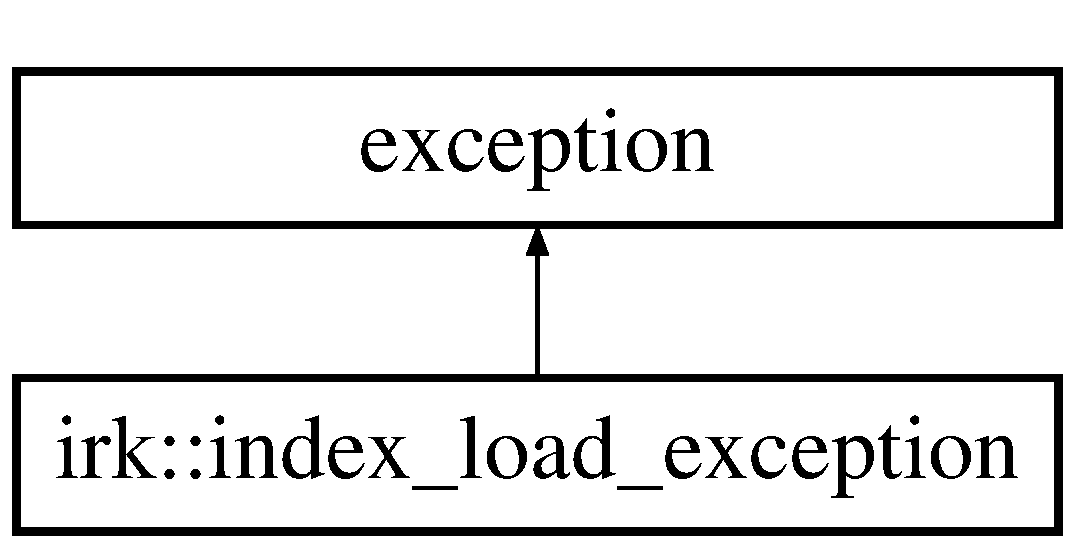
\includegraphics[height=2.000000cm]{structirk_1_1index__load__exception}
\end{center}
\end{figure}
\subsection*{Public Member Functions}
\begin{DoxyCompactItemize}
\item 
\mbox{\hyperlink{structirk_1_1index__load__exception_acd2dcb43dea0e63939f0e264ea4fb9bb}{index\+\_\+load\+\_\+exception}} (fs\+::path \mbox{\hyperlink{structirk_1_1index__load__exception_a38c51abcb6c272187ba08e0c9ad7f674}{file}}, std\+::ios\+\_\+base\+::failure \mbox{\hyperlink{structirk_1_1index__load__exception_aa175d8f2c63df9d2451e57830e2e2467}{reason}})
\item 
const char $\ast$ \mbox{\hyperlink{structirk_1_1index__load__exception_a6c04e64e054848c9de292719d1306c5c}{what}} () const  throw ()
\end{DoxyCompactItemize}
\subsection*{Public Attributes}
\begin{DoxyCompactItemize}
\item 
fs\+::path \mbox{\hyperlink{structirk_1_1index__load__exception_a38c51abcb6c272187ba08e0c9ad7f674}{file}}
\item 
std\+::ios\+\_\+base\+::failure \mbox{\hyperlink{structirk_1_1index__load__exception_aa175d8f2c63df9d2451e57830e2e2467}{reason}}
\end{DoxyCompactItemize}


\subsection{Constructor \& Destructor Documentation}
\mbox{\Hypertarget{structirk_1_1index__load__exception_acd2dcb43dea0e63939f0e264ea4fb9bb}\label{structirk_1_1index__load__exception_acd2dcb43dea0e63939f0e264ea4fb9bb}} 
\index{irk\+::index\+\_\+load\+\_\+exception@{irk\+::index\+\_\+load\+\_\+exception}!index\+\_\+load\+\_\+exception@{index\+\_\+load\+\_\+exception}}
\index{index\+\_\+load\+\_\+exception@{index\+\_\+load\+\_\+exception}!irk\+::index\+\_\+load\+\_\+exception@{irk\+::index\+\_\+load\+\_\+exception}}
\subsubsection{\texorpdfstring{index\+\_\+load\+\_\+exception()}{index\_load\_exception()}}
{\footnotesize\ttfamily irk\+::index\+\_\+load\+\_\+exception\+::index\+\_\+load\+\_\+exception (\begin{DoxyParamCaption}\item[{fs\+::path}]{file,  }\item[{std\+::ios\+\_\+base\+::failure}]{reason }\end{DoxyParamCaption})\hspace{0.3cm}{\ttfamily [inline]}}



\subsection{Member Function Documentation}
\mbox{\Hypertarget{structirk_1_1index__load__exception_a6c04e64e054848c9de292719d1306c5c}\label{structirk_1_1index__load__exception_a6c04e64e054848c9de292719d1306c5c}} 
\index{irk\+::index\+\_\+load\+\_\+exception@{irk\+::index\+\_\+load\+\_\+exception}!what@{what}}
\index{what@{what}!irk\+::index\+\_\+load\+\_\+exception@{irk\+::index\+\_\+load\+\_\+exception}}
\subsubsection{\texorpdfstring{what()}{what()}}
{\footnotesize\ttfamily const char$\ast$ irk\+::index\+\_\+load\+\_\+exception\+::what (\begin{DoxyParamCaption}{ }\end{DoxyParamCaption}) const throw  ) \hspace{0.3cm}{\ttfamily [inline]}}



\subsection{Member Data Documentation}
\mbox{\Hypertarget{structirk_1_1index__load__exception_a38c51abcb6c272187ba08e0c9ad7f674}\label{structirk_1_1index__load__exception_a38c51abcb6c272187ba08e0c9ad7f674}} 
\index{irk\+::index\+\_\+load\+\_\+exception@{irk\+::index\+\_\+load\+\_\+exception}!file@{file}}
\index{file@{file}!irk\+::index\+\_\+load\+\_\+exception@{irk\+::index\+\_\+load\+\_\+exception}}
\subsubsection{\texorpdfstring{file}{file}}
{\footnotesize\ttfamily fs\+::path irk\+::index\+\_\+load\+\_\+exception\+::file}

\mbox{\Hypertarget{structirk_1_1index__load__exception_aa175d8f2c63df9d2451e57830e2e2467}\label{structirk_1_1index__load__exception_aa175d8f2c63df9d2451e57830e2e2467}} 
\index{irk\+::index\+\_\+load\+\_\+exception@{irk\+::index\+\_\+load\+\_\+exception}!reason@{reason}}
\index{reason@{reason}!irk\+::index\+\_\+load\+\_\+exception@{irk\+::index\+\_\+load\+\_\+exception}}
\subsubsection{\texorpdfstring{reason}{reason}}
{\footnotesize\ttfamily std\+::ios\+\_\+base\+::failure irk\+::index\+\_\+load\+\_\+exception\+::reason}



The documentation for this struct was generated from the following file\+:\begin{DoxyCompactItemize}
\item 
include/irkit/\mbox{\hyperlink{irkit_2index_8hpp}{index.\+hpp}}\end{DoxyCompactItemize}

\hypertarget{classirk_1_1index__merger}{}\section{irk\+:\+:index\+\_\+merger$<$ Doc, Term, Term\+Id, Freq $>$ Class Template Reference}
\label{classirk_1_1index__merger}\index{irk\+::index\+\_\+merger$<$ Doc, Term, Term\+Id, Freq $>$@{irk\+::index\+\_\+merger$<$ Doc, Term, Term\+Id, Freq $>$}}


{\ttfamily \#include $<$merger.\+hpp$>$}

\subsection*{Public Types}
\begin{DoxyCompactItemize}
\item 
using \mbox{\hyperlink{classirk_1_1index__merger_ace9b689f5d38f6aeed3ce16f0f1bd260}{document\+\_\+type}} = Doc
\item 
using \mbox{\hyperlink{classirk_1_1index__merger_a2b76203064ec60dc3b0fa662fd8aa3f0}{term\+\_\+type}} = Term
\item 
using \mbox{\hyperlink{classirk_1_1index__merger_a3731db86b5c514a2dd44555c07abe58e}{term\+\_\+id\+\_\+type}} = Term\+Id
\item 
using \mbox{\hyperlink{classirk_1_1index__merger_a6cb409ab2e737118969206ee9b27d147}{frequency\+\_\+type}} = Freq
\item 
using \mbox{\hyperlink{classirk_1_1index__merger_ad218976b86b988db7a72b81f67d352b4}{index\+\_\+type}} = \mbox{\hyperlink{classirk_1_1inverted__index}{inverted\+\_\+index}}$<$ \mbox{\hyperlink{classirk_1_1index__merger_ace9b689f5d38f6aeed3ce16f0f1bd260}{document\+\_\+type}}, \mbox{\hyperlink{classirk_1_1index__merger_a2b76203064ec60dc3b0fa662fd8aa3f0}{term\+\_\+type}}, \mbox{\hyperlink{classirk_1_1index__merger_a3731db86b5c514a2dd44555c07abe58e}{term\+\_\+id\+\_\+type}}, \mbox{\hyperlink{classirk_1_1index__merger_a6cb409ab2e737118969206ee9b27d147}{frequency\+\_\+type}} $>$
\end{DoxyCompactItemize}
\subsection*{Public Member Functions}
\begin{DoxyCompactItemize}
\item 
\mbox{\hyperlink{classirk_1_1index__merger_af76fffe4b1bc16a692b87f07ff046aaa}{index\+\_\+merger}} (fs\+::path target\+\_\+dir, std\+::vector$<$ fs\+::path $>$ indices, bool skip\+\_\+unique=false)
\item 
void \mbox{\hyperlink{classirk_1_1index__merger_a285409fbb9e208ac3ad05076308e2826}{merge\+\_\+term}} (std\+::vector$<$ entry $>$ \&indices)
\item 
void \mbox{\hyperlink{classirk_1_1index__merger_a7109f40e5fc0213d5c72cd3eda9ccaa5}{merge\+\_\+terms}} ()
\item 
void \mbox{\hyperlink{classirk_1_1index__merger_a82a8c5def4100f2cd1be63a037a3a570}{merge\+\_\+titles}} ()
\end{DoxyCompactItemize}


\subsection{Member Typedef Documentation}
\mbox{\Hypertarget{classirk_1_1index__merger_ace9b689f5d38f6aeed3ce16f0f1bd260}\label{classirk_1_1index__merger_ace9b689f5d38f6aeed3ce16f0f1bd260}} 
\index{irk\+::index\+\_\+merger@{irk\+::index\+\_\+merger}!document\+\_\+type@{document\+\_\+type}}
\index{document\+\_\+type@{document\+\_\+type}!irk\+::index\+\_\+merger@{irk\+::index\+\_\+merger}}
\subsubsection{\texorpdfstring{document\+\_\+type}{document\_type}}
{\footnotesize\ttfamily template$<$class Doc  = std\+::size\+\_\+t, class Term  = std\+::string, class Term\+Id  = std\+::size\+\_\+t, class Freq  = std\+::size\+\_\+t$>$ \\
using \mbox{\hyperlink{classirk_1_1index__merger}{irk\+::index\+\_\+merger}}$<$ Doc, Term, Term\+Id, Freq $>$\+::\mbox{\hyperlink{classirk_1_1index__merger_ace9b689f5d38f6aeed3ce16f0f1bd260}{document\+\_\+type}} =  Doc}

\mbox{\Hypertarget{classirk_1_1index__merger_a6cb409ab2e737118969206ee9b27d147}\label{classirk_1_1index__merger_a6cb409ab2e737118969206ee9b27d147}} 
\index{irk\+::index\+\_\+merger@{irk\+::index\+\_\+merger}!frequency\+\_\+type@{frequency\+\_\+type}}
\index{frequency\+\_\+type@{frequency\+\_\+type}!irk\+::index\+\_\+merger@{irk\+::index\+\_\+merger}}
\subsubsection{\texorpdfstring{frequency\+\_\+type}{frequency\_type}}
{\footnotesize\ttfamily template$<$class Doc  = std\+::size\+\_\+t, class Term  = std\+::string, class Term\+Id  = std\+::size\+\_\+t, class Freq  = std\+::size\+\_\+t$>$ \\
using \mbox{\hyperlink{classirk_1_1index__merger}{irk\+::index\+\_\+merger}}$<$ Doc, Term, Term\+Id, Freq $>$\+::\mbox{\hyperlink{classirk_1_1index__merger_a6cb409ab2e737118969206ee9b27d147}{frequency\+\_\+type}} =  Freq}

\mbox{\Hypertarget{classirk_1_1index__merger_ad218976b86b988db7a72b81f67d352b4}\label{classirk_1_1index__merger_ad218976b86b988db7a72b81f67d352b4}} 
\index{irk\+::index\+\_\+merger@{irk\+::index\+\_\+merger}!index\+\_\+type@{index\+\_\+type}}
\index{index\+\_\+type@{index\+\_\+type}!irk\+::index\+\_\+merger@{irk\+::index\+\_\+merger}}
\subsubsection{\texorpdfstring{index\+\_\+type}{index\_type}}
{\footnotesize\ttfamily template$<$class Doc  = std\+::size\+\_\+t, class Term  = std\+::string, class Term\+Id  = std\+::size\+\_\+t, class Freq  = std\+::size\+\_\+t$>$ \\
using \mbox{\hyperlink{classirk_1_1index__merger}{irk\+::index\+\_\+merger}}$<$ Doc, Term, Term\+Id, Freq $>$\+::\mbox{\hyperlink{classirk_1_1index__merger_ad218976b86b988db7a72b81f67d352b4}{index\+\_\+type}} =  \mbox{\hyperlink{classirk_1_1inverted__index}{inverted\+\_\+index}}$<$\mbox{\hyperlink{classirk_1_1index__merger_ace9b689f5d38f6aeed3ce16f0f1bd260}{document\+\_\+type}}, \mbox{\hyperlink{classirk_1_1index__merger_a2b76203064ec60dc3b0fa662fd8aa3f0}{term\+\_\+type}}, \mbox{\hyperlink{classirk_1_1index__merger_a3731db86b5c514a2dd44555c07abe58e}{term\+\_\+id\+\_\+type}}, \mbox{\hyperlink{classirk_1_1index__merger_a6cb409ab2e737118969206ee9b27d147}{frequency\+\_\+type}}$>$}

\mbox{\Hypertarget{classirk_1_1index__merger_a3731db86b5c514a2dd44555c07abe58e}\label{classirk_1_1index__merger_a3731db86b5c514a2dd44555c07abe58e}} 
\index{irk\+::index\+\_\+merger@{irk\+::index\+\_\+merger}!term\+\_\+id\+\_\+type@{term\+\_\+id\+\_\+type}}
\index{term\+\_\+id\+\_\+type@{term\+\_\+id\+\_\+type}!irk\+::index\+\_\+merger@{irk\+::index\+\_\+merger}}
\subsubsection{\texorpdfstring{term\+\_\+id\+\_\+type}{term\_id\_type}}
{\footnotesize\ttfamily template$<$class Doc  = std\+::size\+\_\+t, class Term  = std\+::string, class Term\+Id  = std\+::size\+\_\+t, class Freq  = std\+::size\+\_\+t$>$ \\
using \mbox{\hyperlink{classirk_1_1index__merger}{irk\+::index\+\_\+merger}}$<$ Doc, Term, Term\+Id, Freq $>$\+::\mbox{\hyperlink{classirk_1_1index__merger_a3731db86b5c514a2dd44555c07abe58e}{term\+\_\+id\+\_\+type}} =  Term\+Id}

\mbox{\Hypertarget{classirk_1_1index__merger_a2b76203064ec60dc3b0fa662fd8aa3f0}\label{classirk_1_1index__merger_a2b76203064ec60dc3b0fa662fd8aa3f0}} 
\index{irk\+::index\+\_\+merger@{irk\+::index\+\_\+merger}!term\+\_\+type@{term\+\_\+type}}
\index{term\+\_\+type@{term\+\_\+type}!irk\+::index\+\_\+merger@{irk\+::index\+\_\+merger}}
\subsubsection{\texorpdfstring{term\+\_\+type}{term\_type}}
{\footnotesize\ttfamily template$<$class Doc  = std\+::size\+\_\+t, class Term  = std\+::string, class Term\+Id  = std\+::size\+\_\+t, class Freq  = std\+::size\+\_\+t$>$ \\
using \mbox{\hyperlink{classirk_1_1index__merger}{irk\+::index\+\_\+merger}}$<$ Doc, Term, Term\+Id, Freq $>$\+::\mbox{\hyperlink{classirk_1_1index__merger_a2b76203064ec60dc3b0fa662fd8aa3f0}{term\+\_\+type}} =  Term}



\subsection{Constructor \& Destructor Documentation}
\mbox{\Hypertarget{classirk_1_1index__merger_af76fffe4b1bc16a692b87f07ff046aaa}\label{classirk_1_1index__merger_af76fffe4b1bc16a692b87f07ff046aaa}} 
\index{irk\+::index\+\_\+merger@{irk\+::index\+\_\+merger}!index\+\_\+merger@{index\+\_\+merger}}
\index{index\+\_\+merger@{index\+\_\+merger}!irk\+::index\+\_\+merger@{irk\+::index\+\_\+merger}}
\subsubsection{\texorpdfstring{index\+\_\+merger()}{index\_merger()}}
{\footnotesize\ttfamily template$<$class Doc  = std\+::size\+\_\+t, class Term  = std\+::string, class Term\+Id  = std\+::size\+\_\+t, class Freq  = std\+::size\+\_\+t$>$ \\
\mbox{\hyperlink{classirk_1_1index__merger}{irk\+::index\+\_\+merger}}$<$ Doc, Term, Term\+Id, Freq $>$\+::\mbox{\hyperlink{classirk_1_1index__merger}{index\+\_\+merger}} (\begin{DoxyParamCaption}\item[{fs\+::path}]{target\+\_\+dir,  }\item[{std\+::vector$<$ fs\+::path $>$}]{indices,  }\item[{bool}]{skip\+\_\+unique = {\ttfamily false} }\end{DoxyParamCaption})\hspace{0.3cm}{\ttfamily [inline]}}



\subsection{Member Function Documentation}
\mbox{\Hypertarget{classirk_1_1index__merger_a285409fbb9e208ac3ad05076308e2826}\label{classirk_1_1index__merger_a285409fbb9e208ac3ad05076308e2826}} 
\index{irk\+::index\+\_\+merger@{irk\+::index\+\_\+merger}!merge\+\_\+term@{merge\+\_\+term}}
\index{merge\+\_\+term@{merge\+\_\+term}!irk\+::index\+\_\+merger@{irk\+::index\+\_\+merger}}
\subsubsection{\texorpdfstring{merge\+\_\+term()}{merge\_term()}}
{\footnotesize\ttfamily template$<$class Doc  = std\+::size\+\_\+t, class Term  = std\+::string, class Term\+Id  = std\+::size\+\_\+t, class Freq  = std\+::size\+\_\+t$>$ \\
void \mbox{\hyperlink{classirk_1_1index__merger}{irk\+::index\+\_\+merger}}$<$ Doc, Term, Term\+Id, Freq $>$\+::merge\+\_\+term (\begin{DoxyParamCaption}\item[{std\+::vector$<$ entry $>$ \&}]{indices }\end{DoxyParamCaption})\hspace{0.3cm}{\ttfamily [inline]}}

\mbox{\Hypertarget{classirk_1_1index__merger_a7109f40e5fc0213d5c72cd3eda9ccaa5}\label{classirk_1_1index__merger_a7109f40e5fc0213d5c72cd3eda9ccaa5}} 
\index{irk\+::index\+\_\+merger@{irk\+::index\+\_\+merger}!merge\+\_\+terms@{merge\+\_\+terms}}
\index{merge\+\_\+terms@{merge\+\_\+terms}!irk\+::index\+\_\+merger@{irk\+::index\+\_\+merger}}
\subsubsection{\texorpdfstring{merge\+\_\+terms()}{merge\_terms()}}
{\footnotesize\ttfamily template$<$class Doc  = std\+::size\+\_\+t, class Term  = std\+::string, class Term\+Id  = std\+::size\+\_\+t, class Freq  = std\+::size\+\_\+t$>$ \\
void \mbox{\hyperlink{classirk_1_1index__merger}{irk\+::index\+\_\+merger}}$<$ Doc, Term, Term\+Id, Freq $>$\+::merge\+\_\+terms (\begin{DoxyParamCaption}{ }\end{DoxyParamCaption})\hspace{0.3cm}{\ttfamily [inline]}}

\mbox{\Hypertarget{classirk_1_1index__merger_a82a8c5def4100f2cd1be63a037a3a570}\label{classirk_1_1index__merger_a82a8c5def4100f2cd1be63a037a3a570}} 
\index{irk\+::index\+\_\+merger@{irk\+::index\+\_\+merger}!merge\+\_\+titles@{merge\+\_\+titles}}
\index{merge\+\_\+titles@{merge\+\_\+titles}!irk\+::index\+\_\+merger@{irk\+::index\+\_\+merger}}
\subsubsection{\texorpdfstring{merge\+\_\+titles()}{merge\_titles()}}
{\footnotesize\ttfamily template$<$class Doc  = std\+::size\+\_\+t, class Term  = std\+::string, class Term\+Id  = std\+::size\+\_\+t, class Freq  = std\+::size\+\_\+t$>$ \\
void \mbox{\hyperlink{classirk_1_1index__merger}{irk\+::index\+\_\+merger}}$<$ Doc, Term, Term\+Id, Freq $>$\+::merge\+\_\+titles (\begin{DoxyParamCaption}{ }\end{DoxyParamCaption})\hspace{0.3cm}{\ttfamily [inline]}}



The documentation for this class was generated from the following file\+:\begin{DoxyCompactItemize}
\item 
include/irkit/index/\mbox{\hyperlink{merger_8hpp}{merger.\+hpp}}\end{DoxyCompactItemize}

\hypertarget{classirk_1_1input__bit__stream}{}\section{irk\+:\+:input\+\_\+bit\+\_\+stream Class Reference}
\label{classirk_1_1input__bit__stream}\index{irk\+::input\+\_\+bit\+\_\+stream@{irk\+::input\+\_\+bit\+\_\+stream}}


An input stream reading bits.  




{\ttfamily \#include $<$bitstream.\+hpp$>$}

\subsection*{Public Member Functions}
\begin{DoxyCompactItemize}
\item 
\mbox{\hyperlink{classirk_1_1input__bit__stream_a9265f80a24bee081fdade3d7950f4c12}{input\+\_\+bit\+\_\+stream}} (std\+::istream \&in)
\item 
std\+::int8\+\_\+t \mbox{\hyperlink{classirk_1_1input__bit__stream_a5d0df3f69ce0887e5f93fc15a59f9b96}{read}} ()
\begin{DoxyCompactList}\small\item\em Returns bit\+: 0 or 1, or -\/1 if no bit could be read. \end{DoxyCompactList}\item 
void \mbox{\hyperlink{classirk_1_1input__bit__stream_a470b904afe60107c49105a5d15bd86e2}{clear\+\_\+buffer}} ()
\end{DoxyCompactItemize}
\subsection*{Protected Member Functions}
\begin{DoxyCompactItemize}
\item 
std\+::int8\+\_\+t \mbox{\hyperlink{classirk_1_1input__bit__stream_a8e85aa977d3b47cdb8adc96c688795f3}{get\+\_\+bit}} (unsigned int n)
\end{DoxyCompactItemize}
\subsection*{Protected Attributes}
\begin{DoxyCompactItemize}
\item 
unsigned char \mbox{\hyperlink{classirk_1_1input__bit__stream_a18d1743fba8de3f3ff758f991790f3d3}{byte\+\_\+}} = 0
\item 
std\+::uint8\+\_\+t \mbox{\hyperlink{classirk_1_1input__bit__stream_a1d7126f65850a4f4e7775d8880fe0609}{buffered\+\_\+pos\+\_\+}} = 8
\item 
std\+::istream \& \mbox{\hyperlink{classirk_1_1input__bit__stream_a3513799a1ea6025e9e6fc2c83a530b6a}{in\+\_\+}}
\end{DoxyCompactItemize}


\subsection{Detailed Description}
An input stream reading bits. 

\subsection{Constructor \& Destructor Documentation}
\mbox{\Hypertarget{classirk_1_1input__bit__stream_a9265f80a24bee081fdade3d7950f4c12}\label{classirk_1_1input__bit__stream_a9265f80a24bee081fdade3d7950f4c12}} 
\index{irk\+::input\+\_\+bit\+\_\+stream@{irk\+::input\+\_\+bit\+\_\+stream}!input\+\_\+bit\+\_\+stream@{input\+\_\+bit\+\_\+stream}}
\index{input\+\_\+bit\+\_\+stream@{input\+\_\+bit\+\_\+stream}!irk\+::input\+\_\+bit\+\_\+stream@{irk\+::input\+\_\+bit\+\_\+stream}}
\subsubsection{\texorpdfstring{input\+\_\+bit\+\_\+stream()}{input\_bit\_stream()}}
{\footnotesize\ttfamily irk\+::input\+\_\+bit\+\_\+stream\+::input\+\_\+bit\+\_\+stream (\begin{DoxyParamCaption}\item[{std\+::istream \&}]{in }\end{DoxyParamCaption})\hspace{0.3cm}{\ttfamily [inline]}, {\ttfamily [explicit]}}



\subsection{Member Function Documentation}
\mbox{\Hypertarget{classirk_1_1input__bit__stream_a470b904afe60107c49105a5d15bd86e2}\label{classirk_1_1input__bit__stream_a470b904afe60107c49105a5d15bd86e2}} 
\index{irk\+::input\+\_\+bit\+\_\+stream@{irk\+::input\+\_\+bit\+\_\+stream}!clear\+\_\+buffer@{clear\+\_\+buffer}}
\index{clear\+\_\+buffer@{clear\+\_\+buffer}!irk\+::input\+\_\+bit\+\_\+stream@{irk\+::input\+\_\+bit\+\_\+stream}}
\subsubsection{\texorpdfstring{clear\+\_\+buffer()}{clear\_buffer()}}
{\footnotesize\ttfamily void irk\+::input\+\_\+bit\+\_\+stream\+::clear\+\_\+buffer (\begin{DoxyParamCaption}{ }\end{DoxyParamCaption})\hspace{0.3cm}{\ttfamily [inline]}}

\mbox{\Hypertarget{classirk_1_1input__bit__stream_a8e85aa977d3b47cdb8adc96c688795f3}\label{classirk_1_1input__bit__stream_a8e85aa977d3b47cdb8adc96c688795f3}} 
\index{irk\+::input\+\_\+bit\+\_\+stream@{irk\+::input\+\_\+bit\+\_\+stream}!get\+\_\+bit@{get\+\_\+bit}}
\index{get\+\_\+bit@{get\+\_\+bit}!irk\+::input\+\_\+bit\+\_\+stream@{irk\+::input\+\_\+bit\+\_\+stream}}
\subsubsection{\texorpdfstring{get\+\_\+bit()}{get\_bit()}}
{\footnotesize\ttfamily std\+::int8\+\_\+t irk\+::input\+\_\+bit\+\_\+stream\+::get\+\_\+bit (\begin{DoxyParamCaption}\item[{unsigned int}]{n }\end{DoxyParamCaption})\hspace{0.3cm}{\ttfamily [inline]}, {\ttfamily [protected]}}

\mbox{\Hypertarget{classirk_1_1input__bit__stream_a5d0df3f69ce0887e5f93fc15a59f9b96}\label{classirk_1_1input__bit__stream_a5d0df3f69ce0887e5f93fc15a59f9b96}} 
\index{irk\+::input\+\_\+bit\+\_\+stream@{irk\+::input\+\_\+bit\+\_\+stream}!read@{read}}
\index{read@{read}!irk\+::input\+\_\+bit\+\_\+stream@{irk\+::input\+\_\+bit\+\_\+stream}}
\subsubsection{\texorpdfstring{read()}{read()}}
{\footnotesize\ttfamily std\+::int8\+\_\+t irk\+::input\+\_\+bit\+\_\+stream\+::read (\begin{DoxyParamCaption}{ }\end{DoxyParamCaption})\hspace{0.3cm}{\ttfamily [inline]}}



Returns bit\+: 0 or 1, or -\/1 if no bit could be read. 



\subsection{Member Data Documentation}
\mbox{\Hypertarget{classirk_1_1input__bit__stream_a1d7126f65850a4f4e7775d8880fe0609}\label{classirk_1_1input__bit__stream_a1d7126f65850a4f4e7775d8880fe0609}} 
\index{irk\+::input\+\_\+bit\+\_\+stream@{irk\+::input\+\_\+bit\+\_\+stream}!buffered\+\_\+pos\+\_\+@{buffered\+\_\+pos\+\_\+}}
\index{buffered\+\_\+pos\+\_\+@{buffered\+\_\+pos\+\_\+}!irk\+::input\+\_\+bit\+\_\+stream@{irk\+::input\+\_\+bit\+\_\+stream}}
\subsubsection{\texorpdfstring{buffered\+\_\+pos\+\_\+}{buffered\_pos\_}}
{\footnotesize\ttfamily std\+::uint8\+\_\+t irk\+::input\+\_\+bit\+\_\+stream\+::buffered\+\_\+pos\+\_\+ = 8\hspace{0.3cm}{\ttfamily [protected]}}

\mbox{\Hypertarget{classirk_1_1input__bit__stream_a18d1743fba8de3f3ff758f991790f3d3}\label{classirk_1_1input__bit__stream_a18d1743fba8de3f3ff758f991790f3d3}} 
\index{irk\+::input\+\_\+bit\+\_\+stream@{irk\+::input\+\_\+bit\+\_\+stream}!byte\+\_\+@{byte\+\_\+}}
\index{byte\+\_\+@{byte\+\_\+}!irk\+::input\+\_\+bit\+\_\+stream@{irk\+::input\+\_\+bit\+\_\+stream}}
\subsubsection{\texorpdfstring{byte\+\_\+}{byte\_}}
{\footnotesize\ttfamily unsigned char irk\+::input\+\_\+bit\+\_\+stream\+::byte\+\_\+ = 0\hspace{0.3cm}{\ttfamily [protected]}}

\mbox{\Hypertarget{classirk_1_1input__bit__stream_a3513799a1ea6025e9e6fc2c83a530b6a}\label{classirk_1_1input__bit__stream_a3513799a1ea6025e9e6fc2c83a530b6a}} 
\index{irk\+::input\+\_\+bit\+\_\+stream@{irk\+::input\+\_\+bit\+\_\+stream}!in\+\_\+@{in\+\_\+}}
\index{in\+\_\+@{in\+\_\+}!irk\+::input\+\_\+bit\+\_\+stream@{irk\+::input\+\_\+bit\+\_\+stream}}
\subsubsection{\texorpdfstring{in\+\_\+}{in\_}}
{\footnotesize\ttfamily std\+::istream\& irk\+::input\+\_\+bit\+\_\+stream\+::in\+\_\+\hspace{0.3cm}{\ttfamily [protected]}}



The documentation for this class was generated from the following file\+:\begin{DoxyCompactItemize}
\item 
include/irkit/\mbox{\hyperlink{bitstream_8hpp}{bitstream.\+hpp}}\end{DoxyCompactItemize}

\hypertarget{structirk_1_1concept_1_1InputRange}{}\section{irk\+:\+:concept\+:\+:Input\+Range$<$ R $>$ Struct Template Reference}
\label{structirk_1_1concept_1_1InputRange}\index{irk\+::concept\+::\+Input\+Range$<$ R $>$@{irk\+::concept\+::\+Input\+Range$<$ R $>$}}


{\ttfamily \#include $<$concepts.\+hpp$>$}

\subsection*{Public Types}
\begin{DoxyCompactItemize}
\item 
typedef \mbox{\hyperlink{namespaceirk_a333e3104afd57c79fb0c18b90081520a}{iterator\+\_\+t}}$<$ R $>$ \mbox{\hyperlink{structirk_1_1concept_1_1InputRange_ae371697a8302b5517a872683f0cd457a}{iterator\+\_\+type}}
\end{DoxyCompactItemize}
\subsection*{Public Member Functions}
\begin{DoxyCompactItemize}
\item 
\mbox{\hyperlink{structirk_1_1concept_1_1InputRange_a6330299c4f829cf1bcc9bc1103a660ac}{B\+O\+O\+S\+T\+\_\+\+C\+O\+N\+C\+E\+P\+T\+\_\+\+U\+S\+A\+GE}} (\mbox{\hyperlink{structirk_1_1concept_1_1InputRange}{Input\+Range}})
\end{DoxyCompactItemize}


\subsection{Member Typedef Documentation}
\mbox{\Hypertarget{structirk_1_1concept_1_1InputRange_ae371697a8302b5517a872683f0cd457a}\label{structirk_1_1concept_1_1InputRange_ae371697a8302b5517a872683f0cd457a}} 
\index{irk\+::concept\+::\+Input\+Range@{irk\+::concept\+::\+Input\+Range}!iterator\+\_\+type@{iterator\+\_\+type}}
\index{iterator\+\_\+type@{iterator\+\_\+type}!irk\+::concept\+::\+Input\+Range@{irk\+::concept\+::\+Input\+Range}}
\subsubsection{\texorpdfstring{iterator\+\_\+type}{iterator\_type}}
{\footnotesize\ttfamily template$<$class R $>$ \\
typedef \mbox{\hyperlink{namespaceirk_a333e3104afd57c79fb0c18b90081520a}{iterator\+\_\+t}}$<$R$>$ \mbox{\hyperlink{structirk_1_1concept_1_1InputRange}{irk\+::concept\+::\+Input\+Range}}$<$ R $>$\+::\mbox{\hyperlink{structirk_1_1concept_1_1InputRange_ae371697a8302b5517a872683f0cd457a}{iterator\+\_\+type}}}



\subsection{Member Function Documentation}
\mbox{\Hypertarget{structirk_1_1concept_1_1InputRange_a6330299c4f829cf1bcc9bc1103a660ac}\label{structirk_1_1concept_1_1InputRange_a6330299c4f829cf1bcc9bc1103a660ac}} 
\index{irk\+::concept\+::\+Input\+Range@{irk\+::concept\+::\+Input\+Range}!B\+O\+O\+S\+T\+\_\+\+C\+O\+N\+C\+E\+P\+T\+\_\+\+U\+S\+A\+GE@{B\+O\+O\+S\+T\+\_\+\+C\+O\+N\+C\+E\+P\+T\+\_\+\+U\+S\+A\+GE}}
\index{B\+O\+O\+S\+T\+\_\+\+C\+O\+N\+C\+E\+P\+T\+\_\+\+U\+S\+A\+GE@{B\+O\+O\+S\+T\+\_\+\+C\+O\+N\+C\+E\+P\+T\+\_\+\+U\+S\+A\+GE}!irk\+::concept\+::\+Input\+Range@{irk\+::concept\+::\+Input\+Range}}
\subsubsection{\texorpdfstring{B\+O\+O\+S\+T\+\_\+\+C\+O\+N\+C\+E\+P\+T\+\_\+\+U\+S\+A\+G\+E()}{BOOST\_CONCEPT\_USAGE()}}
{\footnotesize\ttfamily template$<$class R $>$ \\
\mbox{\hyperlink{structirk_1_1concept_1_1InputRange}{irk\+::concept\+::\+Input\+Range}}$<$ R $>$\+::B\+O\+O\+S\+T\+\_\+\+C\+O\+N\+C\+E\+P\+T\+\_\+\+U\+S\+A\+GE (\begin{DoxyParamCaption}\item[{\mbox{\hyperlink{structirk_1_1concept_1_1InputRange}{Input\+Range}}$<$ R $>$}]{ }\end{DoxyParamCaption})\hspace{0.3cm}{\ttfamily [inline]}}



The documentation for this struct was generated from the following file\+:\begin{DoxyCompactItemize}
\item 
include/irkit/\mbox{\hyperlink{concepts_8hpp}{concepts.\+hpp}}\end{DoxyCompactItemize}

\hypertarget{classirk_1_1inverted__index}{}\section{irk\+:\+:inverted\+\_\+index$<$ Doc, Term, Term\+Id, Freq $>$ Class Template Reference}
\label{classirk_1_1inverted__index}\index{irk\+::inverted\+\_\+index$<$ Doc, Term, Term\+Id, Freq $>$@{irk\+::inverted\+\_\+index$<$ Doc, Term, Term\+Id, Freq $>$}}


{\ttfamily \#include $<$index.\+hpp$>$}

\subsection*{Public Types}
\begin{DoxyCompactItemize}
\item 
using \mbox{\hyperlink{classirk_1_1inverted__index_ab708a9d1605de705341f3ed81bd7d5e7}{document\+\_\+type}} = Doc
\item 
using \mbox{\hyperlink{classirk_1_1inverted__index_a7a60c2cec1774c08f21e8e27ccb5ac33}{term\+\_\+type}} = Term
\item 
using \mbox{\hyperlink{classirk_1_1inverted__index_aac7579f5261c795a6f19a7f700b57b2b}{term\+\_\+id\+\_\+type}} = Term\+Id
\item 
using \mbox{\hyperlink{classirk_1_1inverted__index_a549e531087ca14fc58742608cc8fe2e7}{frequency\+\_\+type}} = Freq
\end{DoxyCompactItemize}
\subsection*{Public Member Functions}
\begin{DoxyCompactItemize}
\item 
\mbox{\hyperlink{classirk_1_1inverted__index_aeac9d91ff26a573b8c6aa7f28918a5d7}{inverted\+\_\+index}} (std\+::vector$<$ \mbox{\hyperlink{classirk_1_1inverted__index_a7a60c2cec1774c08f21e8e27ccb5ac33}{term\+\_\+type}} $>$ terms, std\+::vector$<$ Freq $>$ term\+\_\+dfs, std\+::vector$<$ char $>$ doc\+\_\+ids, \mbox{\hyperlink{classirk_1_1offset__table}{offset\+\_\+table}}$<$$>$ doc\+\_\+ids\+\_\+off, std\+::vector$<$ char $>$ doc\+\_\+counts, \mbox{\hyperlink{classirk_1_1offset__table}{offset\+\_\+table}}$<$$>$ doc\+\_\+counts\+\_\+off, std\+::vector$<$ std\+::string $>$ \mbox{\hyperlink{classirk_1_1inverted__index_ac3c5100fced55578e115553c8cda9080}{titles}})
\item 
\mbox{\hyperlink{classirk_1_1inverted__index_a8b9969577ec0556c38ea05d5cc674fb8}{inverted\+\_\+index}} (fs\+::path dir, bool in\+\_\+memory=true, bool skip\+\_\+term\+\_\+map=false, bool verbose=false)
\item 
void \mbox{\hyperlink{classirk_1_1inverted__index_a592cccf4d8b77906e33e90b09f9dec7a}{load\+\_\+properties}} (fs\+::path properties\+\_\+file)
\item 
void \mbox{\hyperlink{classirk_1_1inverted__index_a3c9012991057b448f113bad80d344d68}{load\+\_\+term\+\_\+dfs}} (fs\+::path term\+\_\+df\+\_\+file)
\item 
void \mbox{\hyperlink{classirk_1_1inverted__index_a0b389492f9ab680e28f801590472069c}{load\+\_\+titles}} (fs\+::path titles\+\_\+file)
\item 
void \mbox{\hyperlink{classirk_1_1inverted__index_ad52c3a74f65778de12778dffb3306b62}{load\+\_\+disk\+\_\+term\+\_\+map}} (fs\+::path term\+\_\+map\+\_\+file)
\item 
void \mbox{\hyperlink{classirk_1_1inverted__index_af26ea157a030b67feff19878afbacbdd}{load\+\_\+term\+\_\+map}} (fs\+::path term\+\_\+file)
\item 
void \mbox{\hyperlink{classirk_1_1inverted__index_a231961e5ef231dabb4cd02becb64db5a}{load\+\_\+data}} (fs\+::path data\+\_\+file, std\+::vector$<$ char $>$ \&data\+\_\+container) const
\item 
std\+::size\+\_\+t \mbox{\hyperlink{classirk_1_1inverted__index_a06e5f0eb312766fe8ad96c054a9ec310}{file\+\_\+size}} (fs\+::path file)
\item 
std\+::vector$<$ char $>$ \mbox{\hyperlink{classirk_1_1inverted__index_a66e54902ec83c229af58f1f6b443ed0d}{load\+\_\+data}} (fs\+::path data\+\_\+file, std\+::size\+\_\+t start, std\+::size\+\_\+t size) const
\item 
std\+::size\+\_\+t \mbox{\hyperlink{classirk_1_1inverted__index_a6666e1a0c0facdec6c805abc153a9ea7}{collection\+\_\+size}} () const
\item 
{\footnotesize template$<$class Score\+Fn  = score\+::tf\+\_\+idf\+\_\+scorer$>$ }\\auto \mbox{\hyperlink{classirk_1_1inverted__index_ada3586a485b42d220669d319f6b5acc4}{posting\+\_\+ranges}} (const std\+::vector$<$ std\+::string $>$ \&terms, Score\+Fn score\+\_\+fn=\mbox{\hyperlink{structirk_1_1score_1_1tf__idf__scorer}{score\+::tf\+\_\+idf\+\_\+scorer}}\{\}) const -\/$>$ std\+::vector$<$ \mbox{\hyperlink{namespaceirk_af92c7aae439f59ccae252f027f851c24}{dspr}}$<$ \mbox{\hyperlink{structirk_1_1__posting}{\+\_\+posting}}$<$ \mbox{\hyperlink{classirk_1_1inverted__index_ab708a9d1605de705341f3ed81bd7d5e7}{document\+\_\+type}}, \mbox{\hyperlink{namespaceirk_1_1score_af4a2c84b3548a4ac12aac3862bc94875}{score\+::score\+\_\+result\+\_\+t}}$<$ Score\+Fn, \mbox{\hyperlink{classirk_1_1inverted__index_ab708a9d1605de705341f3ed81bd7d5e7}{document\+\_\+type}}, Freq $>$$>$, Freq, Score\+Fn $>$$>$
\item 
{\footnotesize template$<$class Score\+Fn  = score\+::tf\+\_\+idf\+\_\+scorer$>$ }\\auto \mbox{\hyperlink{classirk_1_1inverted__index_a95a85fe09dae6dfb47cd7bdfa8ce2a4d}{posting\+\_\+range}} (const std\+::string \&\mbox{\hyperlink{classirk_1_1inverted__index_af6d217382bf3bed6b19a009cb0274148}{term}}, Score\+Fn score\+\_\+fn=\mbox{\hyperlink{structirk_1_1score_1_1tf__idf__scorer}{score\+::tf\+\_\+idf\+\_\+scorer}}\{\}) const -\/$>$ \mbox{\hyperlink{namespaceirk_af92c7aae439f59ccae252f027f851c24}{dspr}}$<$ \mbox{\hyperlink{structirk_1_1__posting}{\+\_\+posting}}$<$ \mbox{\hyperlink{classirk_1_1inverted__index_ab708a9d1605de705341f3ed81bd7d5e7}{document\+\_\+type}}, \mbox{\hyperlink{namespaceirk_1_1score_af4a2c84b3548a4ac12aac3862bc94875}{score\+::score\+\_\+result\+\_\+t}}$<$ Score\+Fn, \mbox{\hyperlink{classirk_1_1inverted__index_ab708a9d1605de705341f3ed81bd7d5e7}{document\+\_\+type}}, Freq $>$$>$, Freq, Score\+Fn $>$
\item 
{\footnotesize template$<$class Score\+Fn  = score\+::tf\+\_\+idf\+\_\+scorer$>$ }\\auto \mbox{\hyperlink{classirk_1_1inverted__index_adde74983c6f5bab062296561b3b0b010}{posting\+\_\+range}} (\mbox{\hyperlink{classirk_1_1inverted__index_aac7579f5261c795a6f19a7f700b57b2b}{term\+\_\+id\+\_\+type}} \mbox{\hyperlink{classirk_1_1inverted__index_accd0efb6f27eea7853d45548a6bb0e7d}{term\+\_\+id}}, Score\+Fn score\+\_\+fn=\mbox{\hyperlink{structirk_1_1score_1_1tf__idf__scorer}{score\+::tf\+\_\+idf\+\_\+scorer}}\{\}) const -\/$>$ \mbox{\hyperlink{namespaceirk_af92c7aae439f59ccae252f027f851c24}{dspr}}$<$ \mbox{\hyperlink{structirk_1_1__posting}{\+\_\+posting}}$<$ \mbox{\hyperlink{classirk_1_1inverted__index_ab708a9d1605de705341f3ed81bd7d5e7}{document\+\_\+type}}, \mbox{\hyperlink{namespaceirk_1_1score_af4a2c84b3548a4ac12aac3862bc94875}{score\+::score\+\_\+result\+\_\+t}}$<$ Score\+Fn, \mbox{\hyperlink{classirk_1_1inverted__index_ab708a9d1605de705341f3ed81bd7d5e7}{document\+\_\+type}}, Freq $>$$>$, Freq, Score\+Fn $>$
\item 
std\+::string \mbox{\hyperlink{classirk_1_1inverted__index_aa2aa71522e78ec5e29fa30b56c434702}{title}} (\mbox{\hyperlink{classirk_1_1inverted__index_ab708a9d1605de705341f3ed81bd7d5e7}{document\+\_\+type}} doc\+\_\+id) const
\item 
const std\+::vector$<$ std\+::string $>$ \& \mbox{\hyperlink{classirk_1_1inverted__index_ac3c5100fced55578e115553c8cda9080}{titles}} () const
\item 
\mbox{\hyperlink{classirk_1_1inverted__index_a7a60c2cec1774c08f21e8e27ccb5ac33}{term\+\_\+type}} \mbox{\hyperlink{classirk_1_1inverted__index_af6d217382bf3bed6b19a009cb0274148}{term}} (\mbox{\hyperlink{classirk_1_1inverted__index_aac7579f5261c795a6f19a7f700b57b2b}{term\+\_\+id\+\_\+type}} \mbox{\hyperlink{classirk_1_1inverted__index_accd0efb6f27eea7853d45548a6bb0e7d}{term\+\_\+id}}) const
\item 
std\+::optional$<$ \mbox{\hyperlink{classirk_1_1inverted__index_aac7579f5261c795a6f19a7f700b57b2b}{term\+\_\+id\+\_\+type}} $>$ \mbox{\hyperlink{classirk_1_1inverted__index_accd0efb6f27eea7853d45548a6bb0e7d}{term\+\_\+id}} (\mbox{\hyperlink{classirk_1_1inverted__index_a7a60c2cec1774c08f21e8e27ccb5ac33}{term\+\_\+type}} \mbox{\hyperlink{classirk_1_1inverted__index_af6d217382bf3bed6b19a009cb0274148}{term}}) const
\item 
std\+::size\+\_\+t \mbox{\hyperlink{classirk_1_1inverted__index_a5ae0fe7ce408b154daeadcca6a879ca7}{term\+\_\+count}} () const
\end{DoxyCompactItemize}


\subsection{Member Typedef Documentation}
\mbox{\Hypertarget{classirk_1_1inverted__index_ab708a9d1605de705341f3ed81bd7d5e7}\label{classirk_1_1inverted__index_ab708a9d1605de705341f3ed81bd7d5e7}} 
\index{irk\+::inverted\+\_\+index@{irk\+::inverted\+\_\+index}!document\+\_\+type@{document\+\_\+type}}
\index{document\+\_\+type@{document\+\_\+type}!irk\+::inverted\+\_\+index@{irk\+::inverted\+\_\+index}}
\subsubsection{\texorpdfstring{document\+\_\+type}{document\_type}}
{\footnotesize\ttfamily template$<$class Doc  = std\+::size\+\_\+t, class Term  = std\+::string, class Term\+Id  = std\+::size\+\_\+t, class Freq  = std\+::size\+\_\+t$>$ \\
using \mbox{\hyperlink{classirk_1_1inverted__index}{irk\+::inverted\+\_\+index}}$<$ Doc, Term, Term\+Id, Freq $>$\+::\mbox{\hyperlink{classirk_1_1inverted__index_ab708a9d1605de705341f3ed81bd7d5e7}{document\+\_\+type}} =  Doc}

\mbox{\Hypertarget{classirk_1_1inverted__index_a549e531087ca14fc58742608cc8fe2e7}\label{classirk_1_1inverted__index_a549e531087ca14fc58742608cc8fe2e7}} 
\index{irk\+::inverted\+\_\+index@{irk\+::inverted\+\_\+index}!frequency\+\_\+type@{frequency\+\_\+type}}
\index{frequency\+\_\+type@{frequency\+\_\+type}!irk\+::inverted\+\_\+index@{irk\+::inverted\+\_\+index}}
\subsubsection{\texorpdfstring{frequency\+\_\+type}{frequency\_type}}
{\footnotesize\ttfamily template$<$class Doc  = std\+::size\+\_\+t, class Term  = std\+::string, class Term\+Id  = std\+::size\+\_\+t, class Freq  = std\+::size\+\_\+t$>$ \\
using \mbox{\hyperlink{classirk_1_1inverted__index}{irk\+::inverted\+\_\+index}}$<$ Doc, Term, Term\+Id, Freq $>$\+::\mbox{\hyperlink{classirk_1_1inverted__index_a549e531087ca14fc58742608cc8fe2e7}{frequency\+\_\+type}} =  Freq}

\mbox{\Hypertarget{classirk_1_1inverted__index_aac7579f5261c795a6f19a7f700b57b2b}\label{classirk_1_1inverted__index_aac7579f5261c795a6f19a7f700b57b2b}} 
\index{irk\+::inverted\+\_\+index@{irk\+::inverted\+\_\+index}!term\+\_\+id\+\_\+type@{term\+\_\+id\+\_\+type}}
\index{term\+\_\+id\+\_\+type@{term\+\_\+id\+\_\+type}!irk\+::inverted\+\_\+index@{irk\+::inverted\+\_\+index}}
\subsubsection{\texorpdfstring{term\+\_\+id\+\_\+type}{term\_id\_type}}
{\footnotesize\ttfamily template$<$class Doc  = std\+::size\+\_\+t, class Term  = std\+::string, class Term\+Id  = std\+::size\+\_\+t, class Freq  = std\+::size\+\_\+t$>$ \\
using \mbox{\hyperlink{classirk_1_1inverted__index}{irk\+::inverted\+\_\+index}}$<$ Doc, Term, Term\+Id, Freq $>$\+::\mbox{\hyperlink{classirk_1_1inverted__index_aac7579f5261c795a6f19a7f700b57b2b}{term\+\_\+id\+\_\+type}} =  Term\+Id}

\mbox{\Hypertarget{classirk_1_1inverted__index_a7a60c2cec1774c08f21e8e27ccb5ac33}\label{classirk_1_1inverted__index_a7a60c2cec1774c08f21e8e27ccb5ac33}} 
\index{irk\+::inverted\+\_\+index@{irk\+::inverted\+\_\+index}!term\+\_\+type@{term\+\_\+type}}
\index{term\+\_\+type@{term\+\_\+type}!irk\+::inverted\+\_\+index@{irk\+::inverted\+\_\+index}}
\subsubsection{\texorpdfstring{term\+\_\+type}{term\_type}}
{\footnotesize\ttfamily template$<$class Doc  = std\+::size\+\_\+t, class Term  = std\+::string, class Term\+Id  = std\+::size\+\_\+t, class Freq  = std\+::size\+\_\+t$>$ \\
using \mbox{\hyperlink{classirk_1_1inverted__index}{irk\+::inverted\+\_\+index}}$<$ Doc, Term, Term\+Id, Freq $>$\+::\mbox{\hyperlink{classirk_1_1inverted__index_a7a60c2cec1774c08f21e8e27ccb5ac33}{term\+\_\+type}} =  Term}



\subsection{Constructor \& Destructor Documentation}
\mbox{\Hypertarget{classirk_1_1inverted__index_aeac9d91ff26a573b8c6aa7f28918a5d7}\label{classirk_1_1inverted__index_aeac9d91ff26a573b8c6aa7f28918a5d7}} 
\index{irk\+::inverted\+\_\+index@{irk\+::inverted\+\_\+index}!inverted\+\_\+index@{inverted\+\_\+index}}
\index{inverted\+\_\+index@{inverted\+\_\+index}!irk\+::inverted\+\_\+index@{irk\+::inverted\+\_\+index}}
\subsubsection{\texorpdfstring{inverted\+\_\+index()}{inverted\_index()}\hspace{0.1cm}{\footnotesize\ttfamily [1/2]}}
{\footnotesize\ttfamily template$<$class Doc  = std\+::size\+\_\+t, class Term  = std\+::string, class Term\+Id  = std\+::size\+\_\+t, class Freq  = std\+::size\+\_\+t$>$ \\
\mbox{\hyperlink{classirk_1_1inverted__index}{irk\+::inverted\+\_\+index}}$<$ Doc, Term, Term\+Id, Freq $>$\+::\mbox{\hyperlink{classirk_1_1inverted__index}{inverted\+\_\+index}} (\begin{DoxyParamCaption}\item[{std\+::vector$<$ \mbox{\hyperlink{classirk_1_1inverted__index_a7a60c2cec1774c08f21e8e27ccb5ac33}{term\+\_\+type}} $>$}]{terms,  }\item[{std\+::vector$<$ Freq $>$}]{term\+\_\+dfs,  }\item[{std\+::vector$<$ char $>$}]{doc\+\_\+ids,  }\item[{\mbox{\hyperlink{classirk_1_1offset__table}{offset\+\_\+table}}$<$$>$}]{doc\+\_\+ids\+\_\+off,  }\item[{std\+::vector$<$ char $>$}]{doc\+\_\+counts,  }\item[{\mbox{\hyperlink{classirk_1_1offset__table}{offset\+\_\+table}}$<$$>$}]{doc\+\_\+counts\+\_\+off,  }\item[{std\+::vector$<$ std\+::string $>$}]{titles }\end{DoxyParamCaption})\hspace{0.3cm}{\ttfamily [inline]}}

\mbox{\Hypertarget{classirk_1_1inverted__index_a8b9969577ec0556c38ea05d5cc674fb8}\label{classirk_1_1inverted__index_a8b9969577ec0556c38ea05d5cc674fb8}} 
\index{irk\+::inverted\+\_\+index@{irk\+::inverted\+\_\+index}!inverted\+\_\+index@{inverted\+\_\+index}}
\index{inverted\+\_\+index@{inverted\+\_\+index}!irk\+::inverted\+\_\+index@{irk\+::inverted\+\_\+index}}
\subsubsection{\texorpdfstring{inverted\+\_\+index()}{inverted\_index()}\hspace{0.1cm}{\footnotesize\ttfamily [2/2]}}
{\footnotesize\ttfamily template$<$class Doc  = std\+::size\+\_\+t, class Term  = std\+::string, class Term\+Id  = std\+::size\+\_\+t, class Freq  = std\+::size\+\_\+t$>$ \\
\mbox{\hyperlink{classirk_1_1inverted__index}{irk\+::inverted\+\_\+index}}$<$ Doc, Term, Term\+Id, Freq $>$\+::\mbox{\hyperlink{classirk_1_1inverted__index}{inverted\+\_\+index}} (\begin{DoxyParamCaption}\item[{fs\+::path}]{dir,  }\item[{bool}]{in\+\_\+memory = {\ttfamily true},  }\item[{bool}]{skip\+\_\+term\+\_\+map = {\ttfamily false},  }\item[{bool}]{verbose = {\ttfamily false} }\end{DoxyParamCaption})\hspace{0.3cm}{\ttfamily [inline]}}



\subsection{Member Function Documentation}
\mbox{\Hypertarget{classirk_1_1inverted__index_a6666e1a0c0facdec6c805abc153a9ea7}\label{classirk_1_1inverted__index_a6666e1a0c0facdec6c805abc153a9ea7}} 
\index{irk\+::inverted\+\_\+index@{irk\+::inverted\+\_\+index}!collection\+\_\+size@{collection\+\_\+size}}
\index{collection\+\_\+size@{collection\+\_\+size}!irk\+::inverted\+\_\+index@{irk\+::inverted\+\_\+index}}
\subsubsection{\texorpdfstring{collection\+\_\+size()}{collection\_size()}}
{\footnotesize\ttfamily template$<$class Doc  = std\+::size\+\_\+t, class Term  = std\+::string, class Term\+Id  = std\+::size\+\_\+t, class Freq  = std\+::size\+\_\+t$>$ \\
std\+::size\+\_\+t \mbox{\hyperlink{classirk_1_1inverted__index}{irk\+::inverted\+\_\+index}}$<$ Doc, Term, Term\+Id, Freq $>$\+::collection\+\_\+size (\begin{DoxyParamCaption}{ }\end{DoxyParamCaption}) const\hspace{0.3cm}{\ttfamily [inline]}}

\mbox{\Hypertarget{classirk_1_1inverted__index_a06e5f0eb312766fe8ad96c054a9ec310}\label{classirk_1_1inverted__index_a06e5f0eb312766fe8ad96c054a9ec310}} 
\index{irk\+::inverted\+\_\+index@{irk\+::inverted\+\_\+index}!file\+\_\+size@{file\+\_\+size}}
\index{file\+\_\+size@{file\+\_\+size}!irk\+::inverted\+\_\+index@{irk\+::inverted\+\_\+index}}
\subsubsection{\texorpdfstring{file\+\_\+size()}{file\_size()}}
{\footnotesize\ttfamily template$<$class Doc  = std\+::size\+\_\+t, class Term  = std\+::string, class Term\+Id  = std\+::size\+\_\+t, class Freq  = std\+::size\+\_\+t$>$ \\
std\+::size\+\_\+t \mbox{\hyperlink{classirk_1_1inverted__index}{irk\+::inverted\+\_\+index}}$<$ Doc, Term, Term\+Id, Freq $>$\+::file\+\_\+size (\begin{DoxyParamCaption}\item[{fs\+::path}]{file }\end{DoxyParamCaption})\hspace{0.3cm}{\ttfamily [inline]}}

\mbox{\Hypertarget{classirk_1_1inverted__index_a231961e5ef231dabb4cd02becb64db5a}\label{classirk_1_1inverted__index_a231961e5ef231dabb4cd02becb64db5a}} 
\index{irk\+::inverted\+\_\+index@{irk\+::inverted\+\_\+index}!load\+\_\+data@{load\+\_\+data}}
\index{load\+\_\+data@{load\+\_\+data}!irk\+::inverted\+\_\+index@{irk\+::inverted\+\_\+index}}
\subsubsection{\texorpdfstring{load\+\_\+data()}{load\_data()}\hspace{0.1cm}{\footnotesize\ttfamily [1/2]}}
{\footnotesize\ttfamily template$<$class Doc  = std\+::size\+\_\+t, class Term  = std\+::string, class Term\+Id  = std\+::size\+\_\+t, class Freq  = std\+::size\+\_\+t$>$ \\
void \mbox{\hyperlink{classirk_1_1inverted__index}{irk\+::inverted\+\_\+index}}$<$ Doc, Term, Term\+Id, Freq $>$\+::load\+\_\+data (\begin{DoxyParamCaption}\item[{fs\+::path}]{data\+\_\+file,  }\item[{std\+::vector$<$ char $>$ \&}]{data\+\_\+container }\end{DoxyParamCaption}) const\hspace{0.3cm}{\ttfamily [inline]}}

\mbox{\Hypertarget{classirk_1_1inverted__index_a66e54902ec83c229af58f1f6b443ed0d}\label{classirk_1_1inverted__index_a66e54902ec83c229af58f1f6b443ed0d}} 
\index{irk\+::inverted\+\_\+index@{irk\+::inverted\+\_\+index}!load\+\_\+data@{load\+\_\+data}}
\index{load\+\_\+data@{load\+\_\+data}!irk\+::inverted\+\_\+index@{irk\+::inverted\+\_\+index}}
\subsubsection{\texorpdfstring{load\+\_\+data()}{load\_data()}\hspace{0.1cm}{\footnotesize\ttfamily [2/2]}}
{\footnotesize\ttfamily template$<$class Doc  = std\+::size\+\_\+t, class Term  = std\+::string, class Term\+Id  = std\+::size\+\_\+t, class Freq  = std\+::size\+\_\+t$>$ \\
std\+::vector$<$char$>$ \mbox{\hyperlink{classirk_1_1inverted__index}{irk\+::inverted\+\_\+index}}$<$ Doc, Term, Term\+Id, Freq $>$\+::load\+\_\+data (\begin{DoxyParamCaption}\item[{fs\+::path}]{data\+\_\+file,  }\item[{std\+::size\+\_\+t}]{start,  }\item[{std\+::size\+\_\+t}]{size }\end{DoxyParamCaption}) const\hspace{0.3cm}{\ttfamily [inline]}}

\mbox{\Hypertarget{classirk_1_1inverted__index_ad52c3a74f65778de12778dffb3306b62}\label{classirk_1_1inverted__index_ad52c3a74f65778de12778dffb3306b62}} 
\index{irk\+::inverted\+\_\+index@{irk\+::inverted\+\_\+index}!load\+\_\+disk\+\_\+term\+\_\+map@{load\+\_\+disk\+\_\+term\+\_\+map}}
\index{load\+\_\+disk\+\_\+term\+\_\+map@{load\+\_\+disk\+\_\+term\+\_\+map}!irk\+::inverted\+\_\+index@{irk\+::inverted\+\_\+index}}
\subsubsection{\texorpdfstring{load\+\_\+disk\+\_\+term\+\_\+map()}{load\_disk\_term\_map()}}
{\footnotesize\ttfamily template$<$class Doc  = std\+::size\+\_\+t, class Term  = std\+::string, class Term\+Id  = std\+::size\+\_\+t, class Freq  = std\+::size\+\_\+t$>$ \\
void \mbox{\hyperlink{classirk_1_1inverted__index}{irk\+::inverted\+\_\+index}}$<$ Doc, Term, Term\+Id, Freq $>$\+::load\+\_\+disk\+\_\+term\+\_\+map (\begin{DoxyParamCaption}\item[{fs\+::path}]{term\+\_\+map\+\_\+file }\end{DoxyParamCaption})\hspace{0.3cm}{\ttfamily [inline]}}

\mbox{\Hypertarget{classirk_1_1inverted__index_a592cccf4d8b77906e33e90b09f9dec7a}\label{classirk_1_1inverted__index_a592cccf4d8b77906e33e90b09f9dec7a}} 
\index{irk\+::inverted\+\_\+index@{irk\+::inverted\+\_\+index}!load\+\_\+properties@{load\+\_\+properties}}
\index{load\+\_\+properties@{load\+\_\+properties}!irk\+::inverted\+\_\+index@{irk\+::inverted\+\_\+index}}
\subsubsection{\texorpdfstring{load\+\_\+properties()}{load\_properties()}}
{\footnotesize\ttfamily template$<$class Doc  = std\+::size\+\_\+t, class Term  = std\+::string, class Term\+Id  = std\+::size\+\_\+t, class Freq  = std\+::size\+\_\+t$>$ \\
void \mbox{\hyperlink{classirk_1_1inverted__index}{irk\+::inverted\+\_\+index}}$<$ Doc, Term, Term\+Id, Freq $>$\+::load\+\_\+properties (\begin{DoxyParamCaption}\item[{fs\+::path}]{properties\+\_\+file }\end{DoxyParamCaption})\hspace{0.3cm}{\ttfamily [inline]}}

\mbox{\Hypertarget{classirk_1_1inverted__index_a3c9012991057b448f113bad80d344d68}\label{classirk_1_1inverted__index_a3c9012991057b448f113bad80d344d68}} 
\index{irk\+::inverted\+\_\+index@{irk\+::inverted\+\_\+index}!load\+\_\+term\+\_\+dfs@{load\+\_\+term\+\_\+dfs}}
\index{load\+\_\+term\+\_\+dfs@{load\+\_\+term\+\_\+dfs}!irk\+::inverted\+\_\+index@{irk\+::inverted\+\_\+index}}
\subsubsection{\texorpdfstring{load\+\_\+term\+\_\+dfs()}{load\_term\_dfs()}}
{\footnotesize\ttfamily template$<$class Doc  = std\+::size\+\_\+t, class Term  = std\+::string, class Term\+Id  = std\+::size\+\_\+t, class Freq  = std\+::size\+\_\+t$>$ \\
void \mbox{\hyperlink{classirk_1_1inverted__index}{irk\+::inverted\+\_\+index}}$<$ Doc, Term, Term\+Id, Freq $>$\+::load\+\_\+term\+\_\+dfs (\begin{DoxyParamCaption}\item[{fs\+::path}]{term\+\_\+df\+\_\+file }\end{DoxyParamCaption})\hspace{0.3cm}{\ttfamily [inline]}}

\mbox{\Hypertarget{classirk_1_1inverted__index_af26ea157a030b67feff19878afbacbdd}\label{classirk_1_1inverted__index_af26ea157a030b67feff19878afbacbdd}} 
\index{irk\+::inverted\+\_\+index@{irk\+::inverted\+\_\+index}!load\+\_\+term\+\_\+map@{load\+\_\+term\+\_\+map}}
\index{load\+\_\+term\+\_\+map@{load\+\_\+term\+\_\+map}!irk\+::inverted\+\_\+index@{irk\+::inverted\+\_\+index}}
\subsubsection{\texorpdfstring{load\+\_\+term\+\_\+map()}{load\_term\_map()}}
{\footnotesize\ttfamily template$<$class Doc  = std\+::size\+\_\+t, class Term  = std\+::string, class Term\+Id  = std\+::size\+\_\+t, class Freq  = std\+::size\+\_\+t$>$ \\
void \mbox{\hyperlink{classirk_1_1inverted__index}{irk\+::inverted\+\_\+index}}$<$ Doc, Term, Term\+Id, Freq $>$\+::load\+\_\+term\+\_\+map (\begin{DoxyParamCaption}\item[{fs\+::path}]{term\+\_\+file }\end{DoxyParamCaption})\hspace{0.3cm}{\ttfamily [inline]}}

\mbox{\Hypertarget{classirk_1_1inverted__index_a0b389492f9ab680e28f801590472069c}\label{classirk_1_1inverted__index_a0b389492f9ab680e28f801590472069c}} 
\index{irk\+::inverted\+\_\+index@{irk\+::inverted\+\_\+index}!load\+\_\+titles@{load\+\_\+titles}}
\index{load\+\_\+titles@{load\+\_\+titles}!irk\+::inverted\+\_\+index@{irk\+::inverted\+\_\+index}}
\subsubsection{\texorpdfstring{load\+\_\+titles()}{load\_titles()}}
{\footnotesize\ttfamily template$<$class Doc  = std\+::size\+\_\+t, class Term  = std\+::string, class Term\+Id  = std\+::size\+\_\+t, class Freq  = std\+::size\+\_\+t$>$ \\
void \mbox{\hyperlink{classirk_1_1inverted__index}{irk\+::inverted\+\_\+index}}$<$ Doc, Term, Term\+Id, Freq $>$\+::load\+\_\+titles (\begin{DoxyParamCaption}\item[{fs\+::path}]{titles\+\_\+file }\end{DoxyParamCaption})\hspace{0.3cm}{\ttfamily [inline]}}

\mbox{\Hypertarget{classirk_1_1inverted__index_a95a85fe09dae6dfb47cd7bdfa8ce2a4d}\label{classirk_1_1inverted__index_a95a85fe09dae6dfb47cd7bdfa8ce2a4d}} 
\index{irk\+::inverted\+\_\+index@{irk\+::inverted\+\_\+index}!posting\+\_\+range@{posting\+\_\+range}}
\index{posting\+\_\+range@{posting\+\_\+range}!irk\+::inverted\+\_\+index@{irk\+::inverted\+\_\+index}}
\subsubsection{\texorpdfstring{posting\+\_\+range()}{posting\_range()}\hspace{0.1cm}{\footnotesize\ttfamily [1/2]}}
{\footnotesize\ttfamily template$<$class Doc  = std\+::size\+\_\+t, class Term  = std\+::string, class Term\+Id  = std\+::size\+\_\+t, class Freq  = std\+::size\+\_\+t$>$ \\
template$<$class Score\+Fn  = score\+::tf\+\_\+idf\+\_\+scorer$>$ \\
auto \mbox{\hyperlink{classirk_1_1inverted__index}{irk\+::inverted\+\_\+index}}$<$ Doc, Term, Term\+Id, Freq $>$\+::posting\+\_\+range (\begin{DoxyParamCaption}\item[{const std\+::string \&}]{term,  }\item[{Score\+Fn}]{score\+\_\+fn = {\ttfamily \mbox{\hyperlink{structirk_1_1score_1_1tf__idf__scorer}{score\+::tf\+\_\+idf\+\_\+scorer}}\{\}} }\end{DoxyParamCaption}) const -\/$>$ \mbox{\hyperlink{namespaceirk_af92c7aae439f59ccae252f027f851c24}{dspr}}$<$\mbox{\hyperlink{structirk_1_1__posting}{\+\_\+posting}}$<$\mbox{\hyperlink{classirk_1_1inverted__index_ab708a9d1605de705341f3ed81bd7d5e7}{document\+\_\+type}}, \mbox{\hyperlink{namespaceirk_1_1score_af4a2c84b3548a4ac12aac3862bc94875}{score\+::score\+\_\+result\+\_\+t}}$<$Score\+Fn, \mbox{\hyperlink{classirk_1_1inverted__index_ab708a9d1605de705341f3ed81bd7d5e7}{document\+\_\+type}}, Freq$>$$>$,
            Freq,
            Score\+Fn$>$
    \hspace{0.3cm}{\ttfamily [inline]}}

\mbox{\Hypertarget{classirk_1_1inverted__index_adde74983c6f5bab062296561b3b0b010}\label{classirk_1_1inverted__index_adde74983c6f5bab062296561b3b0b010}} 
\index{irk\+::inverted\+\_\+index@{irk\+::inverted\+\_\+index}!posting\+\_\+range@{posting\+\_\+range}}
\index{posting\+\_\+range@{posting\+\_\+range}!irk\+::inverted\+\_\+index@{irk\+::inverted\+\_\+index}}
\subsubsection{\texorpdfstring{posting\+\_\+range()}{posting\_range()}\hspace{0.1cm}{\footnotesize\ttfamily [2/2]}}
{\footnotesize\ttfamily template$<$class Doc  = std\+::size\+\_\+t, class Term  = std\+::string, class Term\+Id  = std\+::size\+\_\+t, class Freq  = std\+::size\+\_\+t$>$ \\
template$<$class Score\+Fn  = score\+::tf\+\_\+idf\+\_\+scorer$>$ \\
auto \mbox{\hyperlink{classirk_1_1inverted__index}{irk\+::inverted\+\_\+index}}$<$ Doc, Term, Term\+Id, Freq $>$\+::posting\+\_\+range (\begin{DoxyParamCaption}\item[{\mbox{\hyperlink{classirk_1_1inverted__index_aac7579f5261c795a6f19a7f700b57b2b}{term\+\_\+id\+\_\+type}}}]{term\+\_\+id,  }\item[{Score\+Fn}]{score\+\_\+fn = {\ttfamily \mbox{\hyperlink{structirk_1_1score_1_1tf__idf__scorer}{score\+::tf\+\_\+idf\+\_\+scorer}}\{\}} }\end{DoxyParamCaption}) const -\/$>$ \mbox{\hyperlink{namespaceirk_af92c7aae439f59ccae252f027f851c24}{dspr}}$<$\mbox{\hyperlink{structirk_1_1__posting}{\+\_\+posting}}$<$\mbox{\hyperlink{classirk_1_1inverted__index_ab708a9d1605de705341f3ed81bd7d5e7}{document\+\_\+type}},
                    \mbox{\hyperlink{namespaceirk_1_1score_af4a2c84b3548a4ac12aac3862bc94875}{score\+::score\+\_\+result\+\_\+t}}$<$Score\+Fn, \mbox{\hyperlink{classirk_1_1inverted__index_ab708a9d1605de705341f3ed81bd7d5e7}{document\+\_\+type}}, Freq$>$$>$,
            Freq,
            Score\+Fn$>$
    \hspace{0.3cm}{\ttfamily [inline]}}

\mbox{\Hypertarget{classirk_1_1inverted__index_ada3586a485b42d220669d319f6b5acc4}\label{classirk_1_1inverted__index_ada3586a485b42d220669d319f6b5acc4}} 
\index{irk\+::inverted\+\_\+index@{irk\+::inverted\+\_\+index}!posting\+\_\+ranges@{posting\+\_\+ranges}}
\index{posting\+\_\+ranges@{posting\+\_\+ranges}!irk\+::inverted\+\_\+index@{irk\+::inverted\+\_\+index}}
\subsubsection{\texorpdfstring{posting\+\_\+ranges()}{posting\_ranges()}}
{\footnotesize\ttfamily template$<$class Doc  = std\+::size\+\_\+t, class Term  = std\+::string, class Term\+Id  = std\+::size\+\_\+t, class Freq  = std\+::size\+\_\+t$>$ \\
template$<$class Score\+Fn  = score\+::tf\+\_\+idf\+\_\+scorer$>$ \\
auto \mbox{\hyperlink{classirk_1_1inverted__index}{irk\+::inverted\+\_\+index}}$<$ Doc, Term, Term\+Id, Freq $>$\+::posting\+\_\+ranges (\begin{DoxyParamCaption}\item[{const std\+::vector$<$ std\+::string $>$ \&}]{terms,  }\item[{Score\+Fn}]{score\+\_\+fn = {\ttfamily \mbox{\hyperlink{structirk_1_1score_1_1tf__idf__scorer}{score\+::tf\+\_\+idf\+\_\+scorer}}\{\}} }\end{DoxyParamCaption}) const -\/$>$ std\+::vector$<$
            \mbox{\hyperlink{namespaceirk_af92c7aae439f59ccae252f027f851c24}{dspr}}$<$\mbox{\hyperlink{structirk_1_1__posting}{\+\_\+posting}}$<$\mbox{\hyperlink{classirk_1_1inverted__index_ab708a9d1605de705341f3ed81bd7d5e7}{document\+\_\+type}}, \mbox{\hyperlink{namespaceirk_1_1score_af4a2c84b3548a4ac12aac3862bc94875}{score\+::score\+\_\+result\+\_\+t}}$<$Score\+Fn, \mbox{\hyperlink{classirk_1_1inverted__index_ab708a9d1605de705341f3ed81bd7d5e7}{document\+\_\+type}}, Freq$>$$>$,
                Freq,
                Score\+Fn$>$$>$
    \hspace{0.3cm}{\ttfamily [inline]}}

\mbox{\Hypertarget{classirk_1_1inverted__index_af6d217382bf3bed6b19a009cb0274148}\label{classirk_1_1inverted__index_af6d217382bf3bed6b19a009cb0274148}} 
\index{irk\+::inverted\+\_\+index@{irk\+::inverted\+\_\+index}!term@{term}}
\index{term@{term}!irk\+::inverted\+\_\+index@{irk\+::inverted\+\_\+index}}
\subsubsection{\texorpdfstring{term()}{term()}}
{\footnotesize\ttfamily template$<$class Doc  = std\+::size\+\_\+t, class Term  = std\+::string, class Term\+Id  = std\+::size\+\_\+t, class Freq  = std\+::size\+\_\+t$>$ \\
\mbox{\hyperlink{classirk_1_1inverted__index_a7a60c2cec1774c08f21e8e27ccb5ac33}{term\+\_\+type}} \mbox{\hyperlink{classirk_1_1inverted__index}{irk\+::inverted\+\_\+index}}$<$ Doc, Term, Term\+Id, Freq $>$\+::term (\begin{DoxyParamCaption}\item[{\mbox{\hyperlink{classirk_1_1inverted__index_aac7579f5261c795a6f19a7f700b57b2b}{term\+\_\+id\+\_\+type}}}]{term\+\_\+id }\end{DoxyParamCaption}) const\hspace{0.3cm}{\ttfamily [inline]}}

\mbox{\Hypertarget{classirk_1_1inverted__index_a5ae0fe7ce408b154daeadcca6a879ca7}\label{classirk_1_1inverted__index_a5ae0fe7ce408b154daeadcca6a879ca7}} 
\index{irk\+::inverted\+\_\+index@{irk\+::inverted\+\_\+index}!term\+\_\+count@{term\+\_\+count}}
\index{term\+\_\+count@{term\+\_\+count}!irk\+::inverted\+\_\+index@{irk\+::inverted\+\_\+index}}
\subsubsection{\texorpdfstring{term\+\_\+count()}{term\_count()}}
{\footnotesize\ttfamily template$<$class Doc  = std\+::size\+\_\+t, class Term  = std\+::string, class Term\+Id  = std\+::size\+\_\+t, class Freq  = std\+::size\+\_\+t$>$ \\
std\+::size\+\_\+t \mbox{\hyperlink{classirk_1_1inverted__index}{irk\+::inverted\+\_\+index}}$<$ Doc, Term, Term\+Id, Freq $>$\+::term\+\_\+count (\begin{DoxyParamCaption}{ }\end{DoxyParamCaption}) const\hspace{0.3cm}{\ttfamily [inline]}}

\mbox{\Hypertarget{classirk_1_1inverted__index_accd0efb6f27eea7853d45548a6bb0e7d}\label{classirk_1_1inverted__index_accd0efb6f27eea7853d45548a6bb0e7d}} 
\index{irk\+::inverted\+\_\+index@{irk\+::inverted\+\_\+index}!term\+\_\+id@{term\+\_\+id}}
\index{term\+\_\+id@{term\+\_\+id}!irk\+::inverted\+\_\+index@{irk\+::inverted\+\_\+index}}
\subsubsection{\texorpdfstring{term\+\_\+id()}{term\_id()}}
{\footnotesize\ttfamily template$<$class Doc  = std\+::size\+\_\+t, class Term  = std\+::string, class Term\+Id  = std\+::size\+\_\+t, class Freq  = std\+::size\+\_\+t$>$ \\
std\+::optional$<$\mbox{\hyperlink{classirk_1_1inverted__index_aac7579f5261c795a6f19a7f700b57b2b}{term\+\_\+id\+\_\+type}}$>$ \mbox{\hyperlink{classirk_1_1inverted__index}{irk\+::inverted\+\_\+index}}$<$ Doc, Term, Term\+Id, Freq $>$\+::term\+\_\+id (\begin{DoxyParamCaption}\item[{\mbox{\hyperlink{classirk_1_1inverted__index_a7a60c2cec1774c08f21e8e27ccb5ac33}{term\+\_\+type}}}]{term }\end{DoxyParamCaption}) const\hspace{0.3cm}{\ttfamily [inline]}}

\mbox{\Hypertarget{classirk_1_1inverted__index_aa2aa71522e78ec5e29fa30b56c434702}\label{classirk_1_1inverted__index_aa2aa71522e78ec5e29fa30b56c434702}} 
\index{irk\+::inverted\+\_\+index@{irk\+::inverted\+\_\+index}!title@{title}}
\index{title@{title}!irk\+::inverted\+\_\+index@{irk\+::inverted\+\_\+index}}
\subsubsection{\texorpdfstring{title()}{title()}}
{\footnotesize\ttfamily template$<$class Doc  = std\+::size\+\_\+t, class Term  = std\+::string, class Term\+Id  = std\+::size\+\_\+t, class Freq  = std\+::size\+\_\+t$>$ \\
std\+::string \mbox{\hyperlink{classirk_1_1inverted__index}{irk\+::inverted\+\_\+index}}$<$ Doc, Term, Term\+Id, Freq $>$\+::title (\begin{DoxyParamCaption}\item[{\mbox{\hyperlink{classirk_1_1inverted__index_ab708a9d1605de705341f3ed81bd7d5e7}{document\+\_\+type}}}]{doc\+\_\+id }\end{DoxyParamCaption}) const\hspace{0.3cm}{\ttfamily [inline]}}

\mbox{\Hypertarget{classirk_1_1inverted__index_ac3c5100fced55578e115553c8cda9080}\label{classirk_1_1inverted__index_ac3c5100fced55578e115553c8cda9080}} 
\index{irk\+::inverted\+\_\+index@{irk\+::inverted\+\_\+index}!titles@{titles}}
\index{titles@{titles}!irk\+::inverted\+\_\+index@{irk\+::inverted\+\_\+index}}
\subsubsection{\texorpdfstring{titles()}{titles()}}
{\footnotesize\ttfamily template$<$class Doc  = std\+::size\+\_\+t, class Term  = std\+::string, class Term\+Id  = std\+::size\+\_\+t, class Freq  = std\+::size\+\_\+t$>$ \\
const std\+::vector$<$std\+::string$>$\& \mbox{\hyperlink{classirk_1_1inverted__index}{irk\+::inverted\+\_\+index}}$<$ Doc, Term, Term\+Id, Freq $>$\+::titles (\begin{DoxyParamCaption}{ }\end{DoxyParamCaption}) const\hspace{0.3cm}{\ttfamily [inline]}}



The documentation for this class was generated from the following file\+:\begin{DoxyCompactItemize}
\item 
include/irkit/\mbox{\hyperlink{irkit_2index_8hpp}{index.\+hpp}}\end{DoxyCompactItemize}

\hypertarget{classirk_1_1v2_1_1inverted__index__mapped__data__source}{}\section{irk\+:\+:v2\+:\+:inverted\+\_\+index\+\_\+mapped\+\_\+data\+\_\+source Class Reference}
\label{classirk_1_1v2_1_1inverted__index__mapped__data__source}\index{irk\+::v2\+::inverted\+\_\+index\+\_\+mapped\+\_\+data\+\_\+source@{irk\+::v2\+::inverted\+\_\+index\+\_\+mapped\+\_\+data\+\_\+source}}


{\ttfamily \#include $<$index.\+hpp$>$}

\subsection*{Public Member Functions}
\begin{DoxyCompactItemize}
\item 
\mbox{\hyperlink{classirk_1_1v2_1_1inverted__index__mapped__data__source_ac0d35968322d01a287985563b0fe7944}{inverted\+\_\+index\+\_\+mapped\+\_\+data\+\_\+source}} (fs\+::path \mbox{\hyperlink{classirk_1_1v2_1_1inverted__index__mapped__data__source_af8e4ab45e3616f308c50f86b8059d4bc}{dir}}, std\+::optional$<$ std\+::string $>$ score\+\_\+name=std\+::nullopt)
\item 
fs\+::path \mbox{\hyperlink{classirk_1_1v2_1_1inverted__index__mapped__data__source_af8e4ab45e3616f308c50f86b8059d4bc}{dir}} ()
\item 
\mbox{\hyperlink{classirk_1_1memory__view}{memory\+\_\+view}} \mbox{\hyperlink{classirk_1_1v2_1_1inverted__index__mapped__data__source_ab0f63b289b23eff5f3bc45e37fb4caca}{documents\+\_\+view}} () const
\item 
\mbox{\hyperlink{classirk_1_1memory__view}{memory\+\_\+view}} \mbox{\hyperlink{classirk_1_1v2_1_1inverted__index__mapped__data__source_ab8ee89932b98c71d6a04b5cd2c8e88fe}{counts\+\_\+view}} () const
\item 
\mbox{\hyperlink{classirk_1_1memory__view}{memory\+\_\+view}} \mbox{\hyperlink{classirk_1_1v2_1_1inverted__index__mapped__data__source_aea3fe4637b8a95e8450f1a0591e1a76b}{document\+\_\+offsets\+\_\+view}} () const
\item 
\mbox{\hyperlink{classirk_1_1memory__view}{memory\+\_\+view}} \mbox{\hyperlink{classirk_1_1v2_1_1inverted__index__mapped__data__source_a167c16e68633483deea05552d465ff60}{count\+\_\+offsets\+\_\+view}} () const
\item 
\mbox{\hyperlink{classirk_1_1memory__view}{memory\+\_\+view}} \mbox{\hyperlink{classirk_1_1v2_1_1inverted__index__mapped__data__source_a9d8df0423e6890e3086366aa20751be2}{term\+\_\+collection\+\_\+frequencies\+\_\+view}} () const
\item 
\mbox{\hyperlink{classirk_1_1memory__view}{memory\+\_\+view}} \mbox{\hyperlink{classirk_1_1v2_1_1inverted__index__mapped__data__source_a026dbb300791bdf6f454c8107747d11c}{term\+\_\+collection\+\_\+occurrences\+\_\+view}} () const
\item 
\mbox{\hyperlink{classirk_1_1memory__view}{memory\+\_\+view}} \mbox{\hyperlink{classirk_1_1v2_1_1inverted__index__mapped__data__source_afe3e546ffa2720e360e9659e114c03ef}{term\+\_\+map\+\_\+source}} () const
\item 
\mbox{\hyperlink{classirk_1_1memory__view}{memory\+\_\+view}} \mbox{\hyperlink{classirk_1_1v2_1_1inverted__index__mapped__data__source_a3521f951f4988a9a3b56ea004494173b}{title\+\_\+map\+\_\+source}} () const
\item 
\mbox{\hyperlink{classirk_1_1memory__view}{memory\+\_\+view}} \mbox{\hyperlink{classirk_1_1v2_1_1inverted__index__mapped__data__source_acefe6922b50825e26ce4551f70a06bcb}{document\+\_\+sizes\+\_\+view}} () const
\item 
\mbox{\hyperlink{classirk_1_1memory__view}{memory\+\_\+view}} \mbox{\hyperlink{classirk_1_1v2_1_1inverted__index__mapped__data__source_abde799ba197589e717e549d9b0d528ff}{properties\+\_\+view}} () const
\item 
std\+::optional$<$ \mbox{\hyperlink{classirk_1_1memory__view}{memory\+\_\+view}} $>$ \mbox{\hyperlink{classirk_1_1v2_1_1inverted__index__mapped__data__source_a13b8b75bd58b4f903ee1cfb750fa6de2}{scores\+\_\+source}} () const
\item 
std\+::optional$<$ \mbox{\hyperlink{classirk_1_1memory__view}{memory\+\_\+view}} $>$ \mbox{\hyperlink{classirk_1_1v2_1_1inverted__index__mapped__data__source_a78b96380fc44ac8bccbf6a6afad2bced}{score\+\_\+offset\+\_\+source}} () const
\end{DoxyCompactItemize}


\subsection{Constructor \& Destructor Documentation}
\mbox{\Hypertarget{classirk_1_1v2_1_1inverted__index__mapped__data__source_ac0d35968322d01a287985563b0fe7944}\label{classirk_1_1v2_1_1inverted__index__mapped__data__source_ac0d35968322d01a287985563b0fe7944}} 
\index{irk\+::v2\+::inverted\+\_\+index\+\_\+mapped\+\_\+data\+\_\+source@{irk\+::v2\+::inverted\+\_\+index\+\_\+mapped\+\_\+data\+\_\+source}!inverted\+\_\+index\+\_\+mapped\+\_\+data\+\_\+source@{inverted\+\_\+index\+\_\+mapped\+\_\+data\+\_\+source}}
\index{inverted\+\_\+index\+\_\+mapped\+\_\+data\+\_\+source@{inverted\+\_\+index\+\_\+mapped\+\_\+data\+\_\+source}!irk\+::v2\+::inverted\+\_\+index\+\_\+mapped\+\_\+data\+\_\+source@{irk\+::v2\+::inverted\+\_\+index\+\_\+mapped\+\_\+data\+\_\+source}}
\subsubsection{\texorpdfstring{inverted\+\_\+index\+\_\+mapped\+\_\+data\+\_\+source()}{inverted\_index\_mapped\_data\_source()}}
{\footnotesize\ttfamily irk\+::v2\+::inverted\+\_\+index\+\_\+mapped\+\_\+data\+\_\+source\+::inverted\+\_\+index\+\_\+mapped\+\_\+data\+\_\+source (\begin{DoxyParamCaption}\item[{fs\+::path}]{dir,  }\item[{std\+::optional$<$ std\+::string $>$}]{score\+\_\+name = {\ttfamily std\+:\+:nullopt} }\end{DoxyParamCaption})\hspace{0.3cm}{\ttfamily [inline]}, {\ttfamily [explicit]}}



\subsection{Member Function Documentation}
\mbox{\Hypertarget{classirk_1_1v2_1_1inverted__index__mapped__data__source_a167c16e68633483deea05552d465ff60}\label{classirk_1_1v2_1_1inverted__index__mapped__data__source_a167c16e68633483deea05552d465ff60}} 
\index{irk\+::v2\+::inverted\+\_\+index\+\_\+mapped\+\_\+data\+\_\+source@{irk\+::v2\+::inverted\+\_\+index\+\_\+mapped\+\_\+data\+\_\+source}!count\+\_\+offsets\+\_\+view@{count\+\_\+offsets\+\_\+view}}
\index{count\+\_\+offsets\+\_\+view@{count\+\_\+offsets\+\_\+view}!irk\+::v2\+::inverted\+\_\+index\+\_\+mapped\+\_\+data\+\_\+source@{irk\+::v2\+::inverted\+\_\+index\+\_\+mapped\+\_\+data\+\_\+source}}
\subsubsection{\texorpdfstring{count\+\_\+offsets\+\_\+view()}{count\_offsets\_view()}}
{\footnotesize\ttfamily \mbox{\hyperlink{classirk_1_1memory__view}{memory\+\_\+view}} irk\+::v2\+::inverted\+\_\+index\+\_\+mapped\+\_\+data\+\_\+source\+::count\+\_\+offsets\+\_\+view (\begin{DoxyParamCaption}{ }\end{DoxyParamCaption}) const\hspace{0.3cm}{\ttfamily [inline]}}

\mbox{\Hypertarget{classirk_1_1v2_1_1inverted__index__mapped__data__source_ab8ee89932b98c71d6a04b5cd2c8e88fe}\label{classirk_1_1v2_1_1inverted__index__mapped__data__source_ab8ee89932b98c71d6a04b5cd2c8e88fe}} 
\index{irk\+::v2\+::inverted\+\_\+index\+\_\+mapped\+\_\+data\+\_\+source@{irk\+::v2\+::inverted\+\_\+index\+\_\+mapped\+\_\+data\+\_\+source}!counts\+\_\+view@{counts\+\_\+view}}
\index{counts\+\_\+view@{counts\+\_\+view}!irk\+::v2\+::inverted\+\_\+index\+\_\+mapped\+\_\+data\+\_\+source@{irk\+::v2\+::inverted\+\_\+index\+\_\+mapped\+\_\+data\+\_\+source}}
\subsubsection{\texorpdfstring{counts\+\_\+view()}{counts\_view()}}
{\footnotesize\ttfamily \mbox{\hyperlink{classirk_1_1memory__view}{memory\+\_\+view}} irk\+::v2\+::inverted\+\_\+index\+\_\+mapped\+\_\+data\+\_\+source\+::counts\+\_\+view (\begin{DoxyParamCaption}{ }\end{DoxyParamCaption}) const\hspace{0.3cm}{\ttfamily [inline]}}

\mbox{\Hypertarget{classirk_1_1v2_1_1inverted__index__mapped__data__source_af8e4ab45e3616f308c50f86b8059d4bc}\label{classirk_1_1v2_1_1inverted__index__mapped__data__source_af8e4ab45e3616f308c50f86b8059d4bc}} 
\index{irk\+::v2\+::inverted\+\_\+index\+\_\+mapped\+\_\+data\+\_\+source@{irk\+::v2\+::inverted\+\_\+index\+\_\+mapped\+\_\+data\+\_\+source}!dir@{dir}}
\index{dir@{dir}!irk\+::v2\+::inverted\+\_\+index\+\_\+mapped\+\_\+data\+\_\+source@{irk\+::v2\+::inverted\+\_\+index\+\_\+mapped\+\_\+data\+\_\+source}}
\subsubsection{\texorpdfstring{dir()}{dir()}}
{\footnotesize\ttfamily fs\+::path irk\+::v2\+::inverted\+\_\+index\+\_\+mapped\+\_\+data\+\_\+source\+::dir (\begin{DoxyParamCaption}{ }\end{DoxyParamCaption})\hspace{0.3cm}{\ttfamily [inline]}}

\mbox{\Hypertarget{classirk_1_1v2_1_1inverted__index__mapped__data__source_aea3fe4637b8a95e8450f1a0591e1a76b}\label{classirk_1_1v2_1_1inverted__index__mapped__data__source_aea3fe4637b8a95e8450f1a0591e1a76b}} 
\index{irk\+::v2\+::inverted\+\_\+index\+\_\+mapped\+\_\+data\+\_\+source@{irk\+::v2\+::inverted\+\_\+index\+\_\+mapped\+\_\+data\+\_\+source}!document\+\_\+offsets\+\_\+view@{document\+\_\+offsets\+\_\+view}}
\index{document\+\_\+offsets\+\_\+view@{document\+\_\+offsets\+\_\+view}!irk\+::v2\+::inverted\+\_\+index\+\_\+mapped\+\_\+data\+\_\+source@{irk\+::v2\+::inverted\+\_\+index\+\_\+mapped\+\_\+data\+\_\+source}}
\subsubsection{\texorpdfstring{document\+\_\+offsets\+\_\+view()}{document\_offsets\_view()}}
{\footnotesize\ttfamily \mbox{\hyperlink{classirk_1_1memory__view}{memory\+\_\+view}} irk\+::v2\+::inverted\+\_\+index\+\_\+mapped\+\_\+data\+\_\+source\+::document\+\_\+offsets\+\_\+view (\begin{DoxyParamCaption}{ }\end{DoxyParamCaption}) const\hspace{0.3cm}{\ttfamily [inline]}}

\mbox{\Hypertarget{classirk_1_1v2_1_1inverted__index__mapped__data__source_acefe6922b50825e26ce4551f70a06bcb}\label{classirk_1_1v2_1_1inverted__index__mapped__data__source_acefe6922b50825e26ce4551f70a06bcb}} 
\index{irk\+::v2\+::inverted\+\_\+index\+\_\+mapped\+\_\+data\+\_\+source@{irk\+::v2\+::inverted\+\_\+index\+\_\+mapped\+\_\+data\+\_\+source}!document\+\_\+sizes\+\_\+view@{document\+\_\+sizes\+\_\+view}}
\index{document\+\_\+sizes\+\_\+view@{document\+\_\+sizes\+\_\+view}!irk\+::v2\+::inverted\+\_\+index\+\_\+mapped\+\_\+data\+\_\+source@{irk\+::v2\+::inverted\+\_\+index\+\_\+mapped\+\_\+data\+\_\+source}}
\subsubsection{\texorpdfstring{document\+\_\+sizes\+\_\+view()}{document\_sizes\_view()}}
{\footnotesize\ttfamily \mbox{\hyperlink{classirk_1_1memory__view}{memory\+\_\+view}} irk\+::v2\+::inverted\+\_\+index\+\_\+mapped\+\_\+data\+\_\+source\+::document\+\_\+sizes\+\_\+view (\begin{DoxyParamCaption}{ }\end{DoxyParamCaption}) const\hspace{0.3cm}{\ttfamily [inline]}}

\mbox{\Hypertarget{classirk_1_1v2_1_1inverted__index__mapped__data__source_ab0f63b289b23eff5f3bc45e37fb4caca}\label{classirk_1_1v2_1_1inverted__index__mapped__data__source_ab0f63b289b23eff5f3bc45e37fb4caca}} 
\index{irk\+::v2\+::inverted\+\_\+index\+\_\+mapped\+\_\+data\+\_\+source@{irk\+::v2\+::inverted\+\_\+index\+\_\+mapped\+\_\+data\+\_\+source}!documents\+\_\+view@{documents\+\_\+view}}
\index{documents\+\_\+view@{documents\+\_\+view}!irk\+::v2\+::inverted\+\_\+index\+\_\+mapped\+\_\+data\+\_\+source@{irk\+::v2\+::inverted\+\_\+index\+\_\+mapped\+\_\+data\+\_\+source}}
\subsubsection{\texorpdfstring{documents\+\_\+view()}{documents\_view()}}
{\footnotesize\ttfamily \mbox{\hyperlink{classirk_1_1memory__view}{memory\+\_\+view}} irk\+::v2\+::inverted\+\_\+index\+\_\+mapped\+\_\+data\+\_\+source\+::documents\+\_\+view (\begin{DoxyParamCaption}{ }\end{DoxyParamCaption}) const\hspace{0.3cm}{\ttfamily [inline]}}

\mbox{\Hypertarget{classirk_1_1v2_1_1inverted__index__mapped__data__source_abde799ba197589e717e549d9b0d528ff}\label{classirk_1_1v2_1_1inverted__index__mapped__data__source_abde799ba197589e717e549d9b0d528ff}} 
\index{irk\+::v2\+::inverted\+\_\+index\+\_\+mapped\+\_\+data\+\_\+source@{irk\+::v2\+::inverted\+\_\+index\+\_\+mapped\+\_\+data\+\_\+source}!properties\+\_\+view@{properties\+\_\+view}}
\index{properties\+\_\+view@{properties\+\_\+view}!irk\+::v2\+::inverted\+\_\+index\+\_\+mapped\+\_\+data\+\_\+source@{irk\+::v2\+::inverted\+\_\+index\+\_\+mapped\+\_\+data\+\_\+source}}
\subsubsection{\texorpdfstring{properties\+\_\+view()}{properties\_view()}}
{\footnotesize\ttfamily \mbox{\hyperlink{classirk_1_1memory__view}{memory\+\_\+view}} irk\+::v2\+::inverted\+\_\+index\+\_\+mapped\+\_\+data\+\_\+source\+::properties\+\_\+view (\begin{DoxyParamCaption}{ }\end{DoxyParamCaption}) const\hspace{0.3cm}{\ttfamily [inline]}}

\mbox{\Hypertarget{classirk_1_1v2_1_1inverted__index__mapped__data__source_a78b96380fc44ac8bccbf6a6afad2bced}\label{classirk_1_1v2_1_1inverted__index__mapped__data__source_a78b96380fc44ac8bccbf6a6afad2bced}} 
\index{irk\+::v2\+::inverted\+\_\+index\+\_\+mapped\+\_\+data\+\_\+source@{irk\+::v2\+::inverted\+\_\+index\+\_\+mapped\+\_\+data\+\_\+source}!score\+\_\+offset\+\_\+source@{score\+\_\+offset\+\_\+source}}
\index{score\+\_\+offset\+\_\+source@{score\+\_\+offset\+\_\+source}!irk\+::v2\+::inverted\+\_\+index\+\_\+mapped\+\_\+data\+\_\+source@{irk\+::v2\+::inverted\+\_\+index\+\_\+mapped\+\_\+data\+\_\+source}}
\subsubsection{\texorpdfstring{score\+\_\+offset\+\_\+source()}{score\_offset\_source()}}
{\footnotesize\ttfamily std\+::optional$<$\mbox{\hyperlink{classirk_1_1memory__view}{memory\+\_\+view}}$>$ irk\+::v2\+::inverted\+\_\+index\+\_\+mapped\+\_\+data\+\_\+source\+::score\+\_\+offset\+\_\+source (\begin{DoxyParamCaption}{ }\end{DoxyParamCaption}) const\hspace{0.3cm}{\ttfamily [inline]}}

\mbox{\Hypertarget{classirk_1_1v2_1_1inverted__index__mapped__data__source_a13b8b75bd58b4f903ee1cfb750fa6de2}\label{classirk_1_1v2_1_1inverted__index__mapped__data__source_a13b8b75bd58b4f903ee1cfb750fa6de2}} 
\index{irk\+::v2\+::inverted\+\_\+index\+\_\+mapped\+\_\+data\+\_\+source@{irk\+::v2\+::inverted\+\_\+index\+\_\+mapped\+\_\+data\+\_\+source}!scores\+\_\+source@{scores\+\_\+source}}
\index{scores\+\_\+source@{scores\+\_\+source}!irk\+::v2\+::inverted\+\_\+index\+\_\+mapped\+\_\+data\+\_\+source@{irk\+::v2\+::inverted\+\_\+index\+\_\+mapped\+\_\+data\+\_\+source}}
\subsubsection{\texorpdfstring{scores\+\_\+source()}{scores\_source()}}
{\footnotesize\ttfamily std\+::optional$<$\mbox{\hyperlink{classirk_1_1memory__view}{memory\+\_\+view}}$>$ irk\+::v2\+::inverted\+\_\+index\+\_\+mapped\+\_\+data\+\_\+source\+::scores\+\_\+source (\begin{DoxyParamCaption}{ }\end{DoxyParamCaption}) const\hspace{0.3cm}{\ttfamily [inline]}}

\mbox{\Hypertarget{classirk_1_1v2_1_1inverted__index__mapped__data__source_a9d8df0423e6890e3086366aa20751be2}\label{classirk_1_1v2_1_1inverted__index__mapped__data__source_a9d8df0423e6890e3086366aa20751be2}} 
\index{irk\+::v2\+::inverted\+\_\+index\+\_\+mapped\+\_\+data\+\_\+source@{irk\+::v2\+::inverted\+\_\+index\+\_\+mapped\+\_\+data\+\_\+source}!term\+\_\+collection\+\_\+frequencies\+\_\+view@{term\+\_\+collection\+\_\+frequencies\+\_\+view}}
\index{term\+\_\+collection\+\_\+frequencies\+\_\+view@{term\+\_\+collection\+\_\+frequencies\+\_\+view}!irk\+::v2\+::inverted\+\_\+index\+\_\+mapped\+\_\+data\+\_\+source@{irk\+::v2\+::inverted\+\_\+index\+\_\+mapped\+\_\+data\+\_\+source}}
\subsubsection{\texorpdfstring{term\+\_\+collection\+\_\+frequencies\+\_\+view()}{term\_collection\_frequencies\_view()}}
{\footnotesize\ttfamily \mbox{\hyperlink{classirk_1_1memory__view}{memory\+\_\+view}} irk\+::v2\+::inverted\+\_\+index\+\_\+mapped\+\_\+data\+\_\+source\+::term\+\_\+collection\+\_\+frequencies\+\_\+view (\begin{DoxyParamCaption}{ }\end{DoxyParamCaption}) const\hspace{0.3cm}{\ttfamily [inline]}}

\mbox{\Hypertarget{classirk_1_1v2_1_1inverted__index__mapped__data__source_a026dbb300791bdf6f454c8107747d11c}\label{classirk_1_1v2_1_1inverted__index__mapped__data__source_a026dbb300791bdf6f454c8107747d11c}} 
\index{irk\+::v2\+::inverted\+\_\+index\+\_\+mapped\+\_\+data\+\_\+source@{irk\+::v2\+::inverted\+\_\+index\+\_\+mapped\+\_\+data\+\_\+source}!term\+\_\+collection\+\_\+occurrences\+\_\+view@{term\+\_\+collection\+\_\+occurrences\+\_\+view}}
\index{term\+\_\+collection\+\_\+occurrences\+\_\+view@{term\+\_\+collection\+\_\+occurrences\+\_\+view}!irk\+::v2\+::inverted\+\_\+index\+\_\+mapped\+\_\+data\+\_\+source@{irk\+::v2\+::inverted\+\_\+index\+\_\+mapped\+\_\+data\+\_\+source}}
\subsubsection{\texorpdfstring{term\+\_\+collection\+\_\+occurrences\+\_\+view()}{term\_collection\_occurrences\_view()}}
{\footnotesize\ttfamily \mbox{\hyperlink{classirk_1_1memory__view}{memory\+\_\+view}} irk\+::v2\+::inverted\+\_\+index\+\_\+mapped\+\_\+data\+\_\+source\+::term\+\_\+collection\+\_\+occurrences\+\_\+view (\begin{DoxyParamCaption}{ }\end{DoxyParamCaption}) const\hspace{0.3cm}{\ttfamily [inline]}}

\mbox{\Hypertarget{classirk_1_1v2_1_1inverted__index__mapped__data__source_afe3e546ffa2720e360e9659e114c03ef}\label{classirk_1_1v2_1_1inverted__index__mapped__data__source_afe3e546ffa2720e360e9659e114c03ef}} 
\index{irk\+::v2\+::inverted\+\_\+index\+\_\+mapped\+\_\+data\+\_\+source@{irk\+::v2\+::inverted\+\_\+index\+\_\+mapped\+\_\+data\+\_\+source}!term\+\_\+map\+\_\+source@{term\+\_\+map\+\_\+source}}
\index{term\+\_\+map\+\_\+source@{term\+\_\+map\+\_\+source}!irk\+::v2\+::inverted\+\_\+index\+\_\+mapped\+\_\+data\+\_\+source@{irk\+::v2\+::inverted\+\_\+index\+\_\+mapped\+\_\+data\+\_\+source}}
\subsubsection{\texorpdfstring{term\+\_\+map\+\_\+source()}{term\_map\_source()}}
{\footnotesize\ttfamily \mbox{\hyperlink{classirk_1_1memory__view}{memory\+\_\+view}} irk\+::v2\+::inverted\+\_\+index\+\_\+mapped\+\_\+data\+\_\+source\+::term\+\_\+map\+\_\+source (\begin{DoxyParamCaption}{ }\end{DoxyParamCaption}) const\hspace{0.3cm}{\ttfamily [inline]}}

\mbox{\Hypertarget{classirk_1_1v2_1_1inverted__index__mapped__data__source_a3521f951f4988a9a3b56ea004494173b}\label{classirk_1_1v2_1_1inverted__index__mapped__data__source_a3521f951f4988a9a3b56ea004494173b}} 
\index{irk\+::v2\+::inverted\+\_\+index\+\_\+mapped\+\_\+data\+\_\+source@{irk\+::v2\+::inverted\+\_\+index\+\_\+mapped\+\_\+data\+\_\+source}!title\+\_\+map\+\_\+source@{title\+\_\+map\+\_\+source}}
\index{title\+\_\+map\+\_\+source@{title\+\_\+map\+\_\+source}!irk\+::v2\+::inverted\+\_\+index\+\_\+mapped\+\_\+data\+\_\+source@{irk\+::v2\+::inverted\+\_\+index\+\_\+mapped\+\_\+data\+\_\+source}}
\subsubsection{\texorpdfstring{title\+\_\+map\+\_\+source()}{title\_map\_source()}}
{\footnotesize\ttfamily \mbox{\hyperlink{classirk_1_1memory__view}{memory\+\_\+view}} irk\+::v2\+::inverted\+\_\+index\+\_\+mapped\+\_\+data\+\_\+source\+::title\+\_\+map\+\_\+source (\begin{DoxyParamCaption}{ }\end{DoxyParamCaption}) const\hspace{0.3cm}{\ttfamily [inline]}}



The documentation for this class was generated from the following file\+:\begin{DoxyCompactItemize}
\item 
include/irkit/\mbox{\hyperlink{index_8hpp}{index.\+hpp}}\end{DoxyCompactItemize}

\hypertarget{classirk_1_1v2_1_1inverted__index__view}{}\section{irk\+:\+:v2\+:\+:inverted\+\_\+index\+\_\+view Class Reference}
\label{classirk_1_1v2_1_1inverted__index__view}\index{irk\+::v2\+::inverted\+\_\+index\+\_\+view@{irk\+::v2\+::inverted\+\_\+index\+\_\+view}}


{\ttfamily \#include $<$index.\+hpp$>$}

\subsection*{Public Types}
\begin{DoxyCompactItemize}
\item 
using \mbox{\hyperlink{classirk_1_1v2_1_1inverted__index__view_a8441dcf60be934782fdaa9411723700b}{document\+\_\+type}} = long
\item 
using \mbox{\hyperlink{classirk_1_1v2_1_1inverted__index__view_ab52405d4c17e6e82893d2650a56e0a32}{frequency\+\_\+type}} = long
\item 
using \mbox{\hyperlink{classirk_1_1v2_1_1inverted__index__view_aebba8b75ebd7b14d546a29fe925352d6}{size\+\_\+type}} = long
\item 
using \mbox{\hyperlink{classirk_1_1v2_1_1inverted__index__view_a5a1f88560e9fe17b54c7af6e2aa31639}{score\+\_\+type}} = long
\item 
using \mbox{\hyperlink{classirk_1_1v2_1_1inverted__index__view_a360d892dce2f7f984ae98119e6b6eb3e}{offset\+\_\+table\+\_\+type}} = \mbox{\hyperlink{classirk_1_1compact__table}{compact\+\_\+table}}$<$ long, \mbox{\hyperlink{structirk_1_1varbyte__codec}{irk\+::varbyte\+\_\+codec}}$<$ long $>$, \mbox{\hyperlink{classirk_1_1memory__view}{memory\+\_\+view}} $>$
\item 
using \mbox{\hyperlink{classirk_1_1v2_1_1inverted__index__view_ab247a56cfb430693e05ee2ff1d10221e}{frequency\+\_\+table\+\_\+type}} = \mbox{\hyperlink{classirk_1_1compact__table}{compact\+\_\+table}}$<$ \mbox{\hyperlink{classirk_1_1v2_1_1inverted__index__view_ab52405d4c17e6e82893d2650a56e0a32}{frequency\+\_\+type}}, \mbox{\hyperlink{structirk_1_1varbyte__codec}{irk\+::varbyte\+\_\+codec}}$<$ \mbox{\hyperlink{classirk_1_1v2_1_1inverted__index__view_ab52405d4c17e6e82893d2650a56e0a32}{frequency\+\_\+type}} $>$, \mbox{\hyperlink{classirk_1_1memory__view}{memory\+\_\+view}} $>$
\item 
using \mbox{\hyperlink{classirk_1_1v2_1_1inverted__index__view_a4f939f733921ca3f5946288273b427d7}{size\+\_\+table\+\_\+type}} = \mbox{\hyperlink{classirk_1_1compact__table}{compact\+\_\+table}}$<$ long, \mbox{\hyperlink{structirk_1_1varbyte__codec}{irk\+::varbyte\+\_\+codec}}$<$ long $>$, \mbox{\hyperlink{classirk_1_1memory__view}{memory\+\_\+view}} $>$
\item 
using \mbox{\hyperlink{classirk_1_1v2_1_1inverted__index__view_a0dd0327febf8c41ecfd339374c47ce5f}{array\+\_\+stream}} = boost\+::iostreams\+::stream\+\_\+buffer$<$ boost\+::iostreams\+::basic\+\_\+array\+\_\+source$<$ char $>$ $>$
\end{DoxyCompactItemize}
\subsection*{Public Member Functions}
\begin{DoxyCompactItemize}
\item 
\mbox{\hyperlink{classirk_1_1v2_1_1inverted__index__view_a0cd2fbbd65fbab5bef4933aee9cf9059}{inverted\+\_\+index\+\_\+view}} ()=default
\item 
\mbox{\hyperlink{classirk_1_1v2_1_1inverted__index__view_ac1b707ab5ab781fcc6c28e0beadad71f}{inverted\+\_\+index\+\_\+view}} (const \mbox{\hyperlink{classirk_1_1v2_1_1inverted__index__view}{inverted\+\_\+index\+\_\+view}} \&)=default
\item 
\mbox{\hyperlink{classirk_1_1v2_1_1inverted__index__view_a477477a458d97aa3f5842894ccba191d}{inverted\+\_\+index\+\_\+view}} (\mbox{\hyperlink{classirk_1_1v2_1_1inverted__index__view}{inverted\+\_\+index\+\_\+view}} \&\&)=default
\item 
{\footnotesize template$<$class Data\+SourceT $>$ }\\\mbox{\hyperlink{classirk_1_1v2_1_1inverted__index__view_a1aab95c206287bbec6b7c2ab34ffbf92}{inverted\+\_\+index\+\_\+view}} (Data\+SourceT $\ast$data, \mbox{\hyperlink{namespaceirk_a831a3a869cf19601dbfb5c41765a2e87}{any\+\_\+codec}}$<$ \mbox{\hyperlink{classirk_1_1v2_1_1inverted__index__view_a8441dcf60be934782fdaa9411723700b}{document\+\_\+type}} $>$ \mbox{\hyperlink{classirk_1_1v2_1_1inverted__index__view_aaa1f3b7660025d60cdb815268d56334c}{document\+\_\+codec}}, \mbox{\hyperlink{namespaceirk_a831a3a869cf19601dbfb5c41765a2e87}{any\+\_\+codec}}$<$ \mbox{\hyperlink{classirk_1_1v2_1_1inverted__index__view_ab52405d4c17e6e82893d2650a56e0a32}{frequency\+\_\+type}} $>$ \mbox{\hyperlink{classirk_1_1v2_1_1inverted__index__view_aacf229a3a8f3eddb0181cc0df59ada3a}{frequency\+\_\+codec}}, \mbox{\hyperlink{namespaceirk_a831a3a869cf19601dbfb5c41765a2e87}{any\+\_\+codec}}$<$ \mbox{\hyperlink{classirk_1_1v2_1_1inverted__index__view_a5a1f88560e9fe17b54c7af6e2aa31639}{score\+\_\+type}} $>$ score\+\_\+codec)
\item 
\mbox{\hyperlink{classirk_1_1v2_1_1inverted__index__view_aebba8b75ebd7b14d546a29fe925352d6}{size\+\_\+type}} \mbox{\hyperlink{classirk_1_1v2_1_1inverted__index__view_a2b00000b6c8ccb6acb487494d6d0093b}{collection\+\_\+size}} () const
\item 
\mbox{\hyperlink{classirk_1_1v2_1_1inverted__index__view_aebba8b75ebd7b14d546a29fe925352d6}{size\+\_\+type}} \mbox{\hyperlink{classirk_1_1v2_1_1inverted__index__view_ad259487c825b0d3a4fa40cb3b29ccc6e}{document\+\_\+size}} (\mbox{\hyperlink{classirk_1_1v2_1_1inverted__index__view_a8441dcf60be934782fdaa9411723700b}{document\+\_\+type}} doc) const
\item 
auto \mbox{\hyperlink{classirk_1_1v2_1_1inverted__index__view_ab53148e1e271e643013d61f7c815a96d}{documents}} (long \mbox{\hyperlink{classirk_1_1v2_1_1inverted__index__view_aa2dd69651e8d1f90218ff5daabbbe0ab}{term\+\_\+id}}) const
\item 
auto \mbox{\hyperlink{classirk_1_1v2_1_1inverted__index__view_ab09742f5b4edb14da6188e0db717ce06}{frequencies}} (long \mbox{\hyperlink{classirk_1_1v2_1_1inverted__index__view_aa2dd69651e8d1f90218ff5daabbbe0ab}{term\+\_\+id}}) const
\item 
auto \mbox{\hyperlink{classirk_1_1v2_1_1inverted__index__view_af1e3ff71d96f699e0405bdf30598fede}{postings}} (long \mbox{\hyperlink{classirk_1_1v2_1_1inverted__index__view_aa2dd69651e8d1f90218ff5daabbbe0ab}{term\+\_\+id}}) const
\item 
auto \mbox{\hyperlink{classirk_1_1v2_1_1inverted__index__view_ac5232b49a6da53394d0cee20ee7c04e9}{postings}} (const std\+::string \&\mbox{\hyperlink{classirk_1_1v2_1_1inverted__index__view_a7c84123ec294a4a533331f316a3ba2e3}{term}}) const
\item 
auto \mbox{\hyperlink{classirk_1_1v2_1_1inverted__index__view_afb4c98e6d2a700089ebec040544116e5}{scored\+\_\+postings}} (long \mbox{\hyperlink{classirk_1_1v2_1_1inverted__index__view_aa2dd69651e8d1f90218ff5daabbbe0ab}{term\+\_\+id}}) const
\item 
{\footnotesize template$<$class Scorer $>$ }\\Scorer \mbox{\hyperlink{classirk_1_1v2_1_1inverted__index__view_afa7ed76022fafa732e52043a5ffb7428}{term\+\_\+scorer}} (long \mbox{\hyperlink{classirk_1_1v2_1_1inverted__index__view_aa2dd69651e8d1f90218ff5daabbbe0ab}{term\+\_\+id}}) const
\item 
std\+::optional$<$ long $>$ \mbox{\hyperlink{classirk_1_1v2_1_1inverted__index__view_aa2dd69651e8d1f90218ff5daabbbe0ab}{term\+\_\+id}} (const std\+::string \&\mbox{\hyperlink{classirk_1_1v2_1_1inverted__index__view_a7c84123ec294a4a533331f316a3ba2e3}{term}}) const
\item 
std\+::string \mbox{\hyperlink{classirk_1_1v2_1_1inverted__index__view_a7c84123ec294a4a533331f316a3ba2e3}{term}} (const long \&id) const
\item 
long \mbox{\hyperlink{classirk_1_1v2_1_1inverted__index__view_af0ca55da7d671601d894169d2a88693b}{tdf}} (long \mbox{\hyperlink{classirk_1_1v2_1_1inverted__index__view_aa2dd69651e8d1f90218ff5daabbbe0ab}{term\+\_\+id}}) const
\item 
long \mbox{\hyperlink{classirk_1_1v2_1_1inverted__index__view_a155b3ff8825b4f000ff51216ef508dea}{term\+\_\+occurrences}} (long \mbox{\hyperlink{classirk_1_1v2_1_1inverted__index__view_aa2dd69651e8d1f90218ff5daabbbe0ab}{term\+\_\+id}}) const
\item 
long \mbox{\hyperlink{classirk_1_1v2_1_1inverted__index__view_a4fb0266edc385a4b527198d403f0f976}{term\+\_\+count}} () const
\item 
long \mbox{\hyperlink{classirk_1_1v2_1_1inverted__index__view_aeb876faef5e15b4567e3347b871fb978}{occurrences\+\_\+count}} () const
\item 
int \mbox{\hyperlink{classirk_1_1v2_1_1inverted__index__view_a5dc900fb0b8353d0caede65d28e8c66e}{skip\+\_\+block\+\_\+size}} () const
\item 
int \mbox{\hyperlink{classirk_1_1v2_1_1inverted__index__view_a6397e7c10fc74ba36d76491286e98a15}{avg\+\_\+document\+\_\+size}} () const
\item 
const \mbox{\hyperlink{classirk_1_1prefix__map}{prefix\+\_\+map}}$<$ long, std\+::vector$<$ char $>$ $>$ \& \mbox{\hyperlink{classirk_1_1v2_1_1inverted__index__view_a2daebedf75a2ddc8f88c90cd635afe0f}{terms}} () const
\item 
const \mbox{\hyperlink{classirk_1_1prefix__map}{prefix\+\_\+map}}$<$ long, std\+::vector$<$ char $>$ $>$ \& \mbox{\hyperlink{classirk_1_1v2_1_1inverted__index__view_a192e892479d3199aa534ea8e2b4169b0}{titles}} () const
\item 
\mbox{\hyperlink{namespaceirk_a831a3a869cf19601dbfb5c41765a2e87}{any\+\_\+codec}}$<$ \mbox{\hyperlink{classirk_1_1v2_1_1inverted__index__view_a8441dcf60be934782fdaa9411723700b}{document\+\_\+type}} $>$ \mbox{\hyperlink{classirk_1_1v2_1_1inverted__index__view_aaa1f3b7660025d60cdb815268d56334c}{document\+\_\+codec}} ()
\item 
\mbox{\hyperlink{namespaceirk_a831a3a869cf19601dbfb5c41765a2e87}{any\+\_\+codec}}$<$ \mbox{\hyperlink{classirk_1_1v2_1_1inverted__index__view_ab52405d4c17e6e82893d2650a56e0a32}{frequency\+\_\+type}} $>$ \mbox{\hyperlink{classirk_1_1v2_1_1inverted__index__view_aacf229a3a8f3eddb0181cc0df59ada3a}{frequency\+\_\+codec}} ()
\end{DoxyCompactItemize}


\subsection{Member Typedef Documentation}
\mbox{\Hypertarget{classirk_1_1v2_1_1inverted__index__view_a0dd0327febf8c41ecfd339374c47ce5f}\label{classirk_1_1v2_1_1inverted__index__view_a0dd0327febf8c41ecfd339374c47ce5f}} 
\index{irk\+::v2\+::inverted\+\_\+index\+\_\+view@{irk\+::v2\+::inverted\+\_\+index\+\_\+view}!array\+\_\+stream@{array\+\_\+stream}}
\index{array\+\_\+stream@{array\+\_\+stream}!irk\+::v2\+::inverted\+\_\+index\+\_\+view@{irk\+::v2\+::inverted\+\_\+index\+\_\+view}}
\subsubsection{\texorpdfstring{array\+\_\+stream}{array\_stream}}
{\footnotesize\ttfamily using \mbox{\hyperlink{classirk_1_1v2_1_1inverted__index__view_a0dd0327febf8c41ecfd339374c47ce5f}{irk\+::v2\+::inverted\+\_\+index\+\_\+view\+::array\+\_\+stream}} =  boost\+::iostreams\+::stream\+\_\+buffer$<$ boost\+::iostreams\+::basic\+\_\+array\+\_\+source$<$char$>$ $>$}

\mbox{\Hypertarget{classirk_1_1v2_1_1inverted__index__view_a8441dcf60be934782fdaa9411723700b}\label{classirk_1_1v2_1_1inverted__index__view_a8441dcf60be934782fdaa9411723700b}} 
\index{irk\+::v2\+::inverted\+\_\+index\+\_\+view@{irk\+::v2\+::inverted\+\_\+index\+\_\+view}!document\+\_\+type@{document\+\_\+type}}
\index{document\+\_\+type@{document\+\_\+type}!irk\+::v2\+::inverted\+\_\+index\+\_\+view@{irk\+::v2\+::inverted\+\_\+index\+\_\+view}}
\subsubsection{\texorpdfstring{document\+\_\+type}{document\_type}}
{\footnotesize\ttfamily using \mbox{\hyperlink{classirk_1_1v2_1_1inverted__index__view_a8441dcf60be934782fdaa9411723700b}{irk\+::v2\+::inverted\+\_\+index\+\_\+view\+::document\+\_\+type}} =  long}

\mbox{\Hypertarget{classirk_1_1v2_1_1inverted__index__view_ab247a56cfb430693e05ee2ff1d10221e}\label{classirk_1_1v2_1_1inverted__index__view_ab247a56cfb430693e05ee2ff1d10221e}} 
\index{irk\+::v2\+::inverted\+\_\+index\+\_\+view@{irk\+::v2\+::inverted\+\_\+index\+\_\+view}!frequency\+\_\+table\+\_\+type@{frequency\+\_\+table\+\_\+type}}
\index{frequency\+\_\+table\+\_\+type@{frequency\+\_\+table\+\_\+type}!irk\+::v2\+::inverted\+\_\+index\+\_\+view@{irk\+::v2\+::inverted\+\_\+index\+\_\+view}}
\subsubsection{\texorpdfstring{frequency\+\_\+table\+\_\+type}{frequency\_table\_type}}
{\footnotesize\ttfamily using \mbox{\hyperlink{classirk_1_1v2_1_1inverted__index__view_ab247a56cfb430693e05ee2ff1d10221e}{irk\+::v2\+::inverted\+\_\+index\+\_\+view\+::frequency\+\_\+table\+\_\+type}} =  \mbox{\hyperlink{classirk_1_1compact__table}{compact\+\_\+table}}$<$\mbox{\hyperlink{classirk_1_1v2_1_1inverted__index__view_ab52405d4c17e6e82893d2650a56e0a32}{frequency\+\_\+type}}, \mbox{\hyperlink{structirk_1_1varbyte__codec}{irk\+::varbyte\+\_\+codec}}$<$\mbox{\hyperlink{classirk_1_1v2_1_1inverted__index__view_ab52405d4c17e6e82893d2650a56e0a32}{frequency\+\_\+type}}$>$, \mbox{\hyperlink{classirk_1_1memory__view}{memory\+\_\+view}}$>$}

\mbox{\Hypertarget{classirk_1_1v2_1_1inverted__index__view_ab52405d4c17e6e82893d2650a56e0a32}\label{classirk_1_1v2_1_1inverted__index__view_ab52405d4c17e6e82893d2650a56e0a32}} 
\index{irk\+::v2\+::inverted\+\_\+index\+\_\+view@{irk\+::v2\+::inverted\+\_\+index\+\_\+view}!frequency\+\_\+type@{frequency\+\_\+type}}
\index{frequency\+\_\+type@{frequency\+\_\+type}!irk\+::v2\+::inverted\+\_\+index\+\_\+view@{irk\+::v2\+::inverted\+\_\+index\+\_\+view}}
\subsubsection{\texorpdfstring{frequency\+\_\+type}{frequency\_type}}
{\footnotesize\ttfamily using \mbox{\hyperlink{classirk_1_1v2_1_1inverted__index__view_ab52405d4c17e6e82893d2650a56e0a32}{irk\+::v2\+::inverted\+\_\+index\+\_\+view\+::frequency\+\_\+type}} =  long}

\mbox{\Hypertarget{classirk_1_1v2_1_1inverted__index__view_a360d892dce2f7f984ae98119e6b6eb3e}\label{classirk_1_1v2_1_1inverted__index__view_a360d892dce2f7f984ae98119e6b6eb3e}} 
\index{irk\+::v2\+::inverted\+\_\+index\+\_\+view@{irk\+::v2\+::inverted\+\_\+index\+\_\+view}!offset\+\_\+table\+\_\+type@{offset\+\_\+table\+\_\+type}}
\index{offset\+\_\+table\+\_\+type@{offset\+\_\+table\+\_\+type}!irk\+::v2\+::inverted\+\_\+index\+\_\+view@{irk\+::v2\+::inverted\+\_\+index\+\_\+view}}
\subsubsection{\texorpdfstring{offset\+\_\+table\+\_\+type}{offset\_table\_type}}
{\footnotesize\ttfamily using \mbox{\hyperlink{classirk_1_1v2_1_1inverted__index__view_a360d892dce2f7f984ae98119e6b6eb3e}{irk\+::v2\+::inverted\+\_\+index\+\_\+view\+::offset\+\_\+table\+\_\+type}} =  \mbox{\hyperlink{classirk_1_1compact__table}{compact\+\_\+table}}$<$long, \mbox{\hyperlink{structirk_1_1varbyte__codec}{irk\+::varbyte\+\_\+codec}}$<$long$>$, \mbox{\hyperlink{classirk_1_1memory__view}{memory\+\_\+view}}$>$}

\mbox{\Hypertarget{classirk_1_1v2_1_1inverted__index__view_a5a1f88560e9fe17b54c7af6e2aa31639}\label{classirk_1_1v2_1_1inverted__index__view_a5a1f88560e9fe17b54c7af6e2aa31639}} 
\index{irk\+::v2\+::inverted\+\_\+index\+\_\+view@{irk\+::v2\+::inverted\+\_\+index\+\_\+view}!score\+\_\+type@{score\+\_\+type}}
\index{score\+\_\+type@{score\+\_\+type}!irk\+::v2\+::inverted\+\_\+index\+\_\+view@{irk\+::v2\+::inverted\+\_\+index\+\_\+view}}
\subsubsection{\texorpdfstring{score\+\_\+type}{score\_type}}
{\footnotesize\ttfamily using \mbox{\hyperlink{classirk_1_1v2_1_1inverted__index__view_a5a1f88560e9fe17b54c7af6e2aa31639}{irk\+::v2\+::inverted\+\_\+index\+\_\+view\+::score\+\_\+type}} =  long}

\mbox{\Hypertarget{classirk_1_1v2_1_1inverted__index__view_a4f939f733921ca3f5946288273b427d7}\label{classirk_1_1v2_1_1inverted__index__view_a4f939f733921ca3f5946288273b427d7}} 
\index{irk\+::v2\+::inverted\+\_\+index\+\_\+view@{irk\+::v2\+::inverted\+\_\+index\+\_\+view}!size\+\_\+table\+\_\+type@{size\+\_\+table\+\_\+type}}
\index{size\+\_\+table\+\_\+type@{size\+\_\+table\+\_\+type}!irk\+::v2\+::inverted\+\_\+index\+\_\+view@{irk\+::v2\+::inverted\+\_\+index\+\_\+view}}
\subsubsection{\texorpdfstring{size\+\_\+table\+\_\+type}{size\_table\_type}}
{\footnotesize\ttfamily using \mbox{\hyperlink{classirk_1_1v2_1_1inverted__index__view_a4f939f733921ca3f5946288273b427d7}{irk\+::v2\+::inverted\+\_\+index\+\_\+view\+::size\+\_\+table\+\_\+type}} =  \mbox{\hyperlink{classirk_1_1compact__table}{compact\+\_\+table}}$<$long, \mbox{\hyperlink{structirk_1_1varbyte__codec}{irk\+::varbyte\+\_\+codec}}$<$long$>$, \mbox{\hyperlink{classirk_1_1memory__view}{memory\+\_\+view}}$>$}

\mbox{\Hypertarget{classirk_1_1v2_1_1inverted__index__view_aebba8b75ebd7b14d546a29fe925352d6}\label{classirk_1_1v2_1_1inverted__index__view_aebba8b75ebd7b14d546a29fe925352d6}} 
\index{irk\+::v2\+::inverted\+\_\+index\+\_\+view@{irk\+::v2\+::inverted\+\_\+index\+\_\+view}!size\+\_\+type@{size\+\_\+type}}
\index{size\+\_\+type@{size\+\_\+type}!irk\+::v2\+::inverted\+\_\+index\+\_\+view@{irk\+::v2\+::inverted\+\_\+index\+\_\+view}}
\subsubsection{\texorpdfstring{size\+\_\+type}{size\_type}}
{\footnotesize\ttfamily using \mbox{\hyperlink{classirk_1_1v2_1_1inverted__index__view_aebba8b75ebd7b14d546a29fe925352d6}{irk\+::v2\+::inverted\+\_\+index\+\_\+view\+::size\+\_\+type}} =  long}



\subsection{Constructor \& Destructor Documentation}
\mbox{\Hypertarget{classirk_1_1v2_1_1inverted__index__view_a0cd2fbbd65fbab5bef4933aee9cf9059}\label{classirk_1_1v2_1_1inverted__index__view_a0cd2fbbd65fbab5bef4933aee9cf9059}} 
\index{irk\+::v2\+::inverted\+\_\+index\+\_\+view@{irk\+::v2\+::inverted\+\_\+index\+\_\+view}!inverted\+\_\+index\+\_\+view@{inverted\+\_\+index\+\_\+view}}
\index{inverted\+\_\+index\+\_\+view@{inverted\+\_\+index\+\_\+view}!irk\+::v2\+::inverted\+\_\+index\+\_\+view@{irk\+::v2\+::inverted\+\_\+index\+\_\+view}}
\subsubsection{\texorpdfstring{inverted\+\_\+index\+\_\+view()}{inverted\_index\_view()}\hspace{0.1cm}{\footnotesize\ttfamily [1/4]}}
{\footnotesize\ttfamily irk\+::v2\+::inverted\+\_\+index\+\_\+view\+::inverted\+\_\+index\+\_\+view (\begin{DoxyParamCaption}{ }\end{DoxyParamCaption})\hspace{0.3cm}{\ttfamily [default]}}

\mbox{\Hypertarget{classirk_1_1v2_1_1inverted__index__view_ac1b707ab5ab781fcc6c28e0beadad71f}\label{classirk_1_1v2_1_1inverted__index__view_ac1b707ab5ab781fcc6c28e0beadad71f}} 
\index{irk\+::v2\+::inverted\+\_\+index\+\_\+view@{irk\+::v2\+::inverted\+\_\+index\+\_\+view}!inverted\+\_\+index\+\_\+view@{inverted\+\_\+index\+\_\+view}}
\index{inverted\+\_\+index\+\_\+view@{inverted\+\_\+index\+\_\+view}!irk\+::v2\+::inverted\+\_\+index\+\_\+view@{irk\+::v2\+::inverted\+\_\+index\+\_\+view}}
\subsubsection{\texorpdfstring{inverted\+\_\+index\+\_\+view()}{inverted\_index\_view()}\hspace{0.1cm}{\footnotesize\ttfamily [2/4]}}
{\footnotesize\ttfamily irk\+::v2\+::inverted\+\_\+index\+\_\+view\+::inverted\+\_\+index\+\_\+view (\begin{DoxyParamCaption}\item[{const \mbox{\hyperlink{classirk_1_1v2_1_1inverted__index__view}{inverted\+\_\+index\+\_\+view}} \&}]{ }\end{DoxyParamCaption})\hspace{0.3cm}{\ttfamily [default]}}

\mbox{\Hypertarget{classirk_1_1v2_1_1inverted__index__view_a477477a458d97aa3f5842894ccba191d}\label{classirk_1_1v2_1_1inverted__index__view_a477477a458d97aa3f5842894ccba191d}} 
\index{irk\+::v2\+::inverted\+\_\+index\+\_\+view@{irk\+::v2\+::inverted\+\_\+index\+\_\+view}!inverted\+\_\+index\+\_\+view@{inverted\+\_\+index\+\_\+view}}
\index{inverted\+\_\+index\+\_\+view@{inverted\+\_\+index\+\_\+view}!irk\+::v2\+::inverted\+\_\+index\+\_\+view@{irk\+::v2\+::inverted\+\_\+index\+\_\+view}}
\subsubsection{\texorpdfstring{inverted\+\_\+index\+\_\+view()}{inverted\_index\_view()}\hspace{0.1cm}{\footnotesize\ttfamily [3/4]}}
{\footnotesize\ttfamily irk\+::v2\+::inverted\+\_\+index\+\_\+view\+::inverted\+\_\+index\+\_\+view (\begin{DoxyParamCaption}\item[{\mbox{\hyperlink{classirk_1_1v2_1_1inverted__index__view}{inverted\+\_\+index\+\_\+view}} \&\&}]{ }\end{DoxyParamCaption})\hspace{0.3cm}{\ttfamily [default]}}

\mbox{\Hypertarget{classirk_1_1v2_1_1inverted__index__view_a1aab95c206287bbec6b7c2ab34ffbf92}\label{classirk_1_1v2_1_1inverted__index__view_a1aab95c206287bbec6b7c2ab34ffbf92}} 
\index{irk\+::v2\+::inverted\+\_\+index\+\_\+view@{irk\+::v2\+::inverted\+\_\+index\+\_\+view}!inverted\+\_\+index\+\_\+view@{inverted\+\_\+index\+\_\+view}}
\index{inverted\+\_\+index\+\_\+view@{inverted\+\_\+index\+\_\+view}!irk\+::v2\+::inverted\+\_\+index\+\_\+view@{irk\+::v2\+::inverted\+\_\+index\+\_\+view}}
\subsubsection{\texorpdfstring{inverted\+\_\+index\+\_\+view()}{inverted\_index\_view()}\hspace{0.1cm}{\footnotesize\ttfamily [4/4]}}
{\footnotesize\ttfamily template$<$class Data\+SourceT $>$ \\
irk\+::v2\+::inverted\+\_\+index\+\_\+view\+::inverted\+\_\+index\+\_\+view (\begin{DoxyParamCaption}\item[{Data\+SourceT $\ast$}]{data,  }\item[{\mbox{\hyperlink{namespaceirk_a831a3a869cf19601dbfb5c41765a2e87}{any\+\_\+codec}}$<$ \mbox{\hyperlink{classirk_1_1v2_1_1inverted__index__view_a8441dcf60be934782fdaa9411723700b}{document\+\_\+type}} $>$}]{document\+\_\+codec,  }\item[{\mbox{\hyperlink{namespaceirk_a831a3a869cf19601dbfb5c41765a2e87}{any\+\_\+codec}}$<$ \mbox{\hyperlink{classirk_1_1v2_1_1inverted__index__view_ab52405d4c17e6e82893d2650a56e0a32}{frequency\+\_\+type}} $>$}]{frequency\+\_\+codec,  }\item[{\mbox{\hyperlink{namespaceirk_a831a3a869cf19601dbfb5c41765a2e87}{any\+\_\+codec}}$<$ \mbox{\hyperlink{classirk_1_1v2_1_1inverted__index__view_a5a1f88560e9fe17b54c7af6e2aa31639}{score\+\_\+type}} $>$}]{score\+\_\+codec }\end{DoxyParamCaption})\hspace{0.3cm}{\ttfamily [inline]}}



\subsection{Member Function Documentation}
\mbox{\Hypertarget{classirk_1_1v2_1_1inverted__index__view_a6397e7c10fc74ba36d76491286e98a15}\label{classirk_1_1v2_1_1inverted__index__view_a6397e7c10fc74ba36d76491286e98a15}} 
\index{irk\+::v2\+::inverted\+\_\+index\+\_\+view@{irk\+::v2\+::inverted\+\_\+index\+\_\+view}!avg\+\_\+document\+\_\+size@{avg\+\_\+document\+\_\+size}}
\index{avg\+\_\+document\+\_\+size@{avg\+\_\+document\+\_\+size}!irk\+::v2\+::inverted\+\_\+index\+\_\+view@{irk\+::v2\+::inverted\+\_\+index\+\_\+view}}
\subsubsection{\texorpdfstring{avg\+\_\+document\+\_\+size()}{avg\_document\_size()}}
{\footnotesize\ttfamily int irk\+::v2\+::inverted\+\_\+index\+\_\+view\+::avg\+\_\+document\+\_\+size (\begin{DoxyParamCaption}{ }\end{DoxyParamCaption}) const\hspace{0.3cm}{\ttfamily [inline]}}

\mbox{\Hypertarget{classirk_1_1v2_1_1inverted__index__view_a2b00000b6c8ccb6acb487494d6d0093b}\label{classirk_1_1v2_1_1inverted__index__view_a2b00000b6c8ccb6acb487494d6d0093b}} 
\index{irk\+::v2\+::inverted\+\_\+index\+\_\+view@{irk\+::v2\+::inverted\+\_\+index\+\_\+view}!collection\+\_\+size@{collection\+\_\+size}}
\index{collection\+\_\+size@{collection\+\_\+size}!irk\+::v2\+::inverted\+\_\+index\+\_\+view@{irk\+::v2\+::inverted\+\_\+index\+\_\+view}}
\subsubsection{\texorpdfstring{collection\+\_\+size()}{collection\_size()}}
{\footnotesize\ttfamily \mbox{\hyperlink{classirk_1_1v2_1_1inverted__index__view_aebba8b75ebd7b14d546a29fe925352d6}{size\+\_\+type}} irk\+::v2\+::inverted\+\_\+index\+\_\+view\+::collection\+\_\+size (\begin{DoxyParamCaption}{ }\end{DoxyParamCaption}) const\hspace{0.3cm}{\ttfamily [inline]}}

\mbox{\Hypertarget{classirk_1_1v2_1_1inverted__index__view_aaa1f3b7660025d60cdb815268d56334c}\label{classirk_1_1v2_1_1inverted__index__view_aaa1f3b7660025d60cdb815268d56334c}} 
\index{irk\+::v2\+::inverted\+\_\+index\+\_\+view@{irk\+::v2\+::inverted\+\_\+index\+\_\+view}!document\+\_\+codec@{document\+\_\+codec}}
\index{document\+\_\+codec@{document\+\_\+codec}!irk\+::v2\+::inverted\+\_\+index\+\_\+view@{irk\+::v2\+::inverted\+\_\+index\+\_\+view}}
\subsubsection{\texorpdfstring{document\+\_\+codec()}{document\_codec()}}
{\footnotesize\ttfamily \mbox{\hyperlink{namespaceirk_a831a3a869cf19601dbfb5c41765a2e87}{any\+\_\+codec}}$<$\mbox{\hyperlink{classirk_1_1v2_1_1inverted__index__view_a8441dcf60be934782fdaa9411723700b}{document\+\_\+type}}$>$ irk\+::v2\+::inverted\+\_\+index\+\_\+view\+::document\+\_\+codec (\begin{DoxyParamCaption}{ }\end{DoxyParamCaption})\hspace{0.3cm}{\ttfamily [inline]}}

\mbox{\Hypertarget{classirk_1_1v2_1_1inverted__index__view_ad259487c825b0d3a4fa40cb3b29ccc6e}\label{classirk_1_1v2_1_1inverted__index__view_ad259487c825b0d3a4fa40cb3b29ccc6e}} 
\index{irk\+::v2\+::inverted\+\_\+index\+\_\+view@{irk\+::v2\+::inverted\+\_\+index\+\_\+view}!document\+\_\+size@{document\+\_\+size}}
\index{document\+\_\+size@{document\+\_\+size}!irk\+::v2\+::inverted\+\_\+index\+\_\+view@{irk\+::v2\+::inverted\+\_\+index\+\_\+view}}
\subsubsection{\texorpdfstring{document\+\_\+size()}{document\_size()}}
{\footnotesize\ttfamily \mbox{\hyperlink{classirk_1_1v2_1_1inverted__index__view_aebba8b75ebd7b14d546a29fe925352d6}{size\+\_\+type}} irk\+::v2\+::inverted\+\_\+index\+\_\+view\+::document\+\_\+size (\begin{DoxyParamCaption}\item[{\mbox{\hyperlink{classirk_1_1v2_1_1inverted__index__view_a8441dcf60be934782fdaa9411723700b}{document\+\_\+type}}}]{doc }\end{DoxyParamCaption}) const\hspace{0.3cm}{\ttfamily [inline]}}

\mbox{\Hypertarget{classirk_1_1v2_1_1inverted__index__view_ab53148e1e271e643013d61f7c815a96d}\label{classirk_1_1v2_1_1inverted__index__view_ab53148e1e271e643013d61f7c815a96d}} 
\index{irk\+::v2\+::inverted\+\_\+index\+\_\+view@{irk\+::v2\+::inverted\+\_\+index\+\_\+view}!documents@{documents}}
\index{documents@{documents}!irk\+::v2\+::inverted\+\_\+index\+\_\+view@{irk\+::v2\+::inverted\+\_\+index\+\_\+view}}
\subsubsection{\texorpdfstring{documents()}{documents()}}
{\footnotesize\ttfamily auto irk\+::v2\+::inverted\+\_\+index\+\_\+view\+::documents (\begin{DoxyParamCaption}\item[{long}]{term\+\_\+id }\end{DoxyParamCaption}) const\hspace{0.3cm}{\ttfamily [inline]}}

\mbox{\Hypertarget{classirk_1_1v2_1_1inverted__index__view_ab09742f5b4edb14da6188e0db717ce06}\label{classirk_1_1v2_1_1inverted__index__view_ab09742f5b4edb14da6188e0db717ce06}} 
\index{irk\+::v2\+::inverted\+\_\+index\+\_\+view@{irk\+::v2\+::inverted\+\_\+index\+\_\+view}!frequencies@{frequencies}}
\index{frequencies@{frequencies}!irk\+::v2\+::inverted\+\_\+index\+\_\+view@{irk\+::v2\+::inverted\+\_\+index\+\_\+view}}
\subsubsection{\texorpdfstring{frequencies()}{frequencies()}}
{\footnotesize\ttfamily auto irk\+::v2\+::inverted\+\_\+index\+\_\+view\+::frequencies (\begin{DoxyParamCaption}\item[{long}]{term\+\_\+id }\end{DoxyParamCaption}) const\hspace{0.3cm}{\ttfamily [inline]}}

\mbox{\Hypertarget{classirk_1_1v2_1_1inverted__index__view_aacf229a3a8f3eddb0181cc0df59ada3a}\label{classirk_1_1v2_1_1inverted__index__view_aacf229a3a8f3eddb0181cc0df59ada3a}} 
\index{irk\+::v2\+::inverted\+\_\+index\+\_\+view@{irk\+::v2\+::inverted\+\_\+index\+\_\+view}!frequency\+\_\+codec@{frequency\+\_\+codec}}
\index{frequency\+\_\+codec@{frequency\+\_\+codec}!irk\+::v2\+::inverted\+\_\+index\+\_\+view@{irk\+::v2\+::inverted\+\_\+index\+\_\+view}}
\subsubsection{\texorpdfstring{frequency\+\_\+codec()}{frequency\_codec()}}
{\footnotesize\ttfamily \mbox{\hyperlink{namespaceirk_a831a3a869cf19601dbfb5c41765a2e87}{any\+\_\+codec}}$<$\mbox{\hyperlink{classirk_1_1v2_1_1inverted__index__view_ab52405d4c17e6e82893d2650a56e0a32}{frequency\+\_\+type}}$>$ irk\+::v2\+::inverted\+\_\+index\+\_\+view\+::frequency\+\_\+codec (\begin{DoxyParamCaption}{ }\end{DoxyParamCaption})\hspace{0.3cm}{\ttfamily [inline]}}

\mbox{\Hypertarget{classirk_1_1v2_1_1inverted__index__view_aeb876faef5e15b4567e3347b871fb978}\label{classirk_1_1v2_1_1inverted__index__view_aeb876faef5e15b4567e3347b871fb978}} 
\index{irk\+::v2\+::inverted\+\_\+index\+\_\+view@{irk\+::v2\+::inverted\+\_\+index\+\_\+view}!occurrences\+\_\+count@{occurrences\+\_\+count}}
\index{occurrences\+\_\+count@{occurrences\+\_\+count}!irk\+::v2\+::inverted\+\_\+index\+\_\+view@{irk\+::v2\+::inverted\+\_\+index\+\_\+view}}
\subsubsection{\texorpdfstring{occurrences\+\_\+count()}{occurrences\_count()}}
{\footnotesize\ttfamily long irk\+::v2\+::inverted\+\_\+index\+\_\+view\+::occurrences\+\_\+count (\begin{DoxyParamCaption}{ }\end{DoxyParamCaption}) const\hspace{0.3cm}{\ttfamily [inline]}}

\mbox{\Hypertarget{classirk_1_1v2_1_1inverted__index__view_af1e3ff71d96f699e0405bdf30598fede}\label{classirk_1_1v2_1_1inverted__index__view_af1e3ff71d96f699e0405bdf30598fede}} 
\index{irk\+::v2\+::inverted\+\_\+index\+\_\+view@{irk\+::v2\+::inverted\+\_\+index\+\_\+view}!postings@{postings}}
\index{postings@{postings}!irk\+::v2\+::inverted\+\_\+index\+\_\+view@{irk\+::v2\+::inverted\+\_\+index\+\_\+view}}
\subsubsection{\texorpdfstring{postings()}{postings()}\hspace{0.1cm}{\footnotesize\ttfamily [1/2]}}
{\footnotesize\ttfamily auto irk\+::v2\+::inverted\+\_\+index\+\_\+view\+::postings (\begin{DoxyParamCaption}\item[{long}]{term\+\_\+id }\end{DoxyParamCaption}) const\hspace{0.3cm}{\ttfamily [inline]}}

\mbox{\Hypertarget{classirk_1_1v2_1_1inverted__index__view_ac5232b49a6da53394d0cee20ee7c04e9}\label{classirk_1_1v2_1_1inverted__index__view_ac5232b49a6da53394d0cee20ee7c04e9}} 
\index{irk\+::v2\+::inverted\+\_\+index\+\_\+view@{irk\+::v2\+::inverted\+\_\+index\+\_\+view}!postings@{postings}}
\index{postings@{postings}!irk\+::v2\+::inverted\+\_\+index\+\_\+view@{irk\+::v2\+::inverted\+\_\+index\+\_\+view}}
\subsubsection{\texorpdfstring{postings()}{postings()}\hspace{0.1cm}{\footnotesize\ttfamily [2/2]}}
{\footnotesize\ttfamily auto irk\+::v2\+::inverted\+\_\+index\+\_\+view\+::postings (\begin{DoxyParamCaption}\item[{const std\+::string \&}]{term }\end{DoxyParamCaption}) const\hspace{0.3cm}{\ttfamily [inline]}}

\mbox{\Hypertarget{classirk_1_1v2_1_1inverted__index__view_afb4c98e6d2a700089ebec040544116e5}\label{classirk_1_1v2_1_1inverted__index__view_afb4c98e6d2a700089ebec040544116e5}} 
\index{irk\+::v2\+::inverted\+\_\+index\+\_\+view@{irk\+::v2\+::inverted\+\_\+index\+\_\+view}!scored\+\_\+postings@{scored\+\_\+postings}}
\index{scored\+\_\+postings@{scored\+\_\+postings}!irk\+::v2\+::inverted\+\_\+index\+\_\+view@{irk\+::v2\+::inverted\+\_\+index\+\_\+view}}
\subsubsection{\texorpdfstring{scored\+\_\+postings()}{scored\_postings()}}
{\footnotesize\ttfamily auto irk\+::v2\+::inverted\+\_\+index\+\_\+view\+::scored\+\_\+postings (\begin{DoxyParamCaption}\item[{long}]{term\+\_\+id }\end{DoxyParamCaption}) const\hspace{0.3cm}{\ttfamily [inline]}}

\mbox{\Hypertarget{classirk_1_1v2_1_1inverted__index__view_a5dc900fb0b8353d0caede65d28e8c66e}\label{classirk_1_1v2_1_1inverted__index__view_a5dc900fb0b8353d0caede65d28e8c66e}} 
\index{irk\+::v2\+::inverted\+\_\+index\+\_\+view@{irk\+::v2\+::inverted\+\_\+index\+\_\+view}!skip\+\_\+block\+\_\+size@{skip\+\_\+block\+\_\+size}}
\index{skip\+\_\+block\+\_\+size@{skip\+\_\+block\+\_\+size}!irk\+::v2\+::inverted\+\_\+index\+\_\+view@{irk\+::v2\+::inverted\+\_\+index\+\_\+view}}
\subsubsection{\texorpdfstring{skip\+\_\+block\+\_\+size()}{skip\_block\_size()}}
{\footnotesize\ttfamily int irk\+::v2\+::inverted\+\_\+index\+\_\+view\+::skip\+\_\+block\+\_\+size (\begin{DoxyParamCaption}{ }\end{DoxyParamCaption}) const\hspace{0.3cm}{\ttfamily [inline]}}

\mbox{\Hypertarget{classirk_1_1v2_1_1inverted__index__view_af0ca55da7d671601d894169d2a88693b}\label{classirk_1_1v2_1_1inverted__index__view_af0ca55da7d671601d894169d2a88693b}} 
\index{irk\+::v2\+::inverted\+\_\+index\+\_\+view@{irk\+::v2\+::inverted\+\_\+index\+\_\+view}!tdf@{tdf}}
\index{tdf@{tdf}!irk\+::v2\+::inverted\+\_\+index\+\_\+view@{irk\+::v2\+::inverted\+\_\+index\+\_\+view}}
\subsubsection{\texorpdfstring{tdf()}{tdf()}}
{\footnotesize\ttfamily long irk\+::v2\+::inverted\+\_\+index\+\_\+view\+::tdf (\begin{DoxyParamCaption}\item[{long}]{term\+\_\+id }\end{DoxyParamCaption}) const\hspace{0.3cm}{\ttfamily [inline]}}

\mbox{\Hypertarget{classirk_1_1v2_1_1inverted__index__view_a7c84123ec294a4a533331f316a3ba2e3}\label{classirk_1_1v2_1_1inverted__index__view_a7c84123ec294a4a533331f316a3ba2e3}} 
\index{irk\+::v2\+::inverted\+\_\+index\+\_\+view@{irk\+::v2\+::inverted\+\_\+index\+\_\+view}!term@{term}}
\index{term@{term}!irk\+::v2\+::inverted\+\_\+index\+\_\+view@{irk\+::v2\+::inverted\+\_\+index\+\_\+view}}
\subsubsection{\texorpdfstring{term()}{term()}}
{\footnotesize\ttfamily std\+::string irk\+::v2\+::inverted\+\_\+index\+\_\+view\+::term (\begin{DoxyParamCaption}\item[{const long \&}]{id }\end{DoxyParamCaption}) const\hspace{0.3cm}{\ttfamily [inline]}}

\mbox{\Hypertarget{classirk_1_1v2_1_1inverted__index__view_a4fb0266edc385a4b527198d403f0f976}\label{classirk_1_1v2_1_1inverted__index__view_a4fb0266edc385a4b527198d403f0f976}} 
\index{irk\+::v2\+::inverted\+\_\+index\+\_\+view@{irk\+::v2\+::inverted\+\_\+index\+\_\+view}!term\+\_\+count@{term\+\_\+count}}
\index{term\+\_\+count@{term\+\_\+count}!irk\+::v2\+::inverted\+\_\+index\+\_\+view@{irk\+::v2\+::inverted\+\_\+index\+\_\+view}}
\subsubsection{\texorpdfstring{term\+\_\+count()}{term\_count()}}
{\footnotesize\ttfamily long irk\+::v2\+::inverted\+\_\+index\+\_\+view\+::term\+\_\+count (\begin{DoxyParamCaption}{ }\end{DoxyParamCaption}) const\hspace{0.3cm}{\ttfamily [inline]}}

\mbox{\Hypertarget{classirk_1_1v2_1_1inverted__index__view_aa2dd69651e8d1f90218ff5daabbbe0ab}\label{classirk_1_1v2_1_1inverted__index__view_aa2dd69651e8d1f90218ff5daabbbe0ab}} 
\index{irk\+::v2\+::inverted\+\_\+index\+\_\+view@{irk\+::v2\+::inverted\+\_\+index\+\_\+view}!term\+\_\+id@{term\+\_\+id}}
\index{term\+\_\+id@{term\+\_\+id}!irk\+::v2\+::inverted\+\_\+index\+\_\+view@{irk\+::v2\+::inverted\+\_\+index\+\_\+view}}
\subsubsection{\texorpdfstring{term\+\_\+id()}{term\_id()}}
{\footnotesize\ttfamily std\+::optional$<$long$>$ irk\+::v2\+::inverted\+\_\+index\+\_\+view\+::term\+\_\+id (\begin{DoxyParamCaption}\item[{const std\+::string \&}]{term }\end{DoxyParamCaption}) const\hspace{0.3cm}{\ttfamily [inline]}}

\mbox{\Hypertarget{classirk_1_1v2_1_1inverted__index__view_a155b3ff8825b4f000ff51216ef508dea}\label{classirk_1_1v2_1_1inverted__index__view_a155b3ff8825b4f000ff51216ef508dea}} 
\index{irk\+::v2\+::inverted\+\_\+index\+\_\+view@{irk\+::v2\+::inverted\+\_\+index\+\_\+view}!term\+\_\+occurrences@{term\+\_\+occurrences}}
\index{term\+\_\+occurrences@{term\+\_\+occurrences}!irk\+::v2\+::inverted\+\_\+index\+\_\+view@{irk\+::v2\+::inverted\+\_\+index\+\_\+view}}
\subsubsection{\texorpdfstring{term\+\_\+occurrences()}{term\_occurrences()}}
{\footnotesize\ttfamily long irk\+::v2\+::inverted\+\_\+index\+\_\+view\+::term\+\_\+occurrences (\begin{DoxyParamCaption}\item[{long}]{term\+\_\+id }\end{DoxyParamCaption}) const\hspace{0.3cm}{\ttfamily [inline]}}

\mbox{\Hypertarget{classirk_1_1v2_1_1inverted__index__view_afa7ed76022fafa732e52043a5ffb7428}\label{classirk_1_1v2_1_1inverted__index__view_afa7ed76022fafa732e52043a5ffb7428}} 
\index{irk\+::v2\+::inverted\+\_\+index\+\_\+view@{irk\+::v2\+::inverted\+\_\+index\+\_\+view}!term\+\_\+scorer@{term\+\_\+scorer}}
\index{term\+\_\+scorer@{term\+\_\+scorer}!irk\+::v2\+::inverted\+\_\+index\+\_\+view@{irk\+::v2\+::inverted\+\_\+index\+\_\+view}}
\subsubsection{\texorpdfstring{term\+\_\+scorer()}{term\_scorer()}}
{\footnotesize\ttfamily template$<$class Scorer $>$ \\
Scorer irk\+::v2\+::inverted\+\_\+index\+\_\+view\+::term\+\_\+scorer (\begin{DoxyParamCaption}\item[{long}]{term\+\_\+id }\end{DoxyParamCaption}) const\hspace{0.3cm}{\ttfamily [inline]}}

\mbox{\Hypertarget{classirk_1_1v2_1_1inverted__index__view_a2daebedf75a2ddc8f88c90cd635afe0f}\label{classirk_1_1v2_1_1inverted__index__view_a2daebedf75a2ddc8f88c90cd635afe0f}} 
\index{irk\+::v2\+::inverted\+\_\+index\+\_\+view@{irk\+::v2\+::inverted\+\_\+index\+\_\+view}!terms@{terms}}
\index{terms@{terms}!irk\+::v2\+::inverted\+\_\+index\+\_\+view@{irk\+::v2\+::inverted\+\_\+index\+\_\+view}}
\subsubsection{\texorpdfstring{terms()}{terms()}}
{\footnotesize\ttfamily const \mbox{\hyperlink{classirk_1_1prefix__map}{prefix\+\_\+map}}$<$long, std\+::vector$<$char$>$ $>$\& irk\+::v2\+::inverted\+\_\+index\+\_\+view\+::terms (\begin{DoxyParamCaption}{ }\end{DoxyParamCaption}) const\hspace{0.3cm}{\ttfamily [inline]}}

\mbox{\Hypertarget{classirk_1_1v2_1_1inverted__index__view_a192e892479d3199aa534ea8e2b4169b0}\label{classirk_1_1v2_1_1inverted__index__view_a192e892479d3199aa534ea8e2b4169b0}} 
\index{irk\+::v2\+::inverted\+\_\+index\+\_\+view@{irk\+::v2\+::inverted\+\_\+index\+\_\+view}!titles@{titles}}
\index{titles@{titles}!irk\+::v2\+::inverted\+\_\+index\+\_\+view@{irk\+::v2\+::inverted\+\_\+index\+\_\+view}}
\subsubsection{\texorpdfstring{titles()}{titles()}}
{\footnotesize\ttfamily const \mbox{\hyperlink{classirk_1_1prefix__map}{prefix\+\_\+map}}$<$long, std\+::vector$<$char$>$ $>$\& irk\+::v2\+::inverted\+\_\+index\+\_\+view\+::titles (\begin{DoxyParamCaption}{ }\end{DoxyParamCaption}) const\hspace{0.3cm}{\ttfamily [inline]}}



The documentation for this class was generated from the following file\+:\begin{DoxyCompactItemize}
\item 
include/irkit/\mbox{\hyperlink{index_8hpp}{index.\+hpp}}\end{DoxyCompactItemize}

\hypertarget{classirk_1_1memory__view_1_1iterator}{}\section{irk\+:\+:memory\+\_\+view\+:\+:iterator Class Reference}
\label{classirk_1_1memory__view_1_1iterator}\index{irk\+::memory\+\_\+view\+::iterator@{irk\+::memory\+\_\+view\+::iterator}}


Character iterator.  




{\ttfamily \#include $<$memoryview.\+hpp$>$}

Inheritance diagram for irk\+:\+:memory\+\_\+view\+:\+:iterator\+:\begin{figure}[H]
\begin{center}
\leavevmode
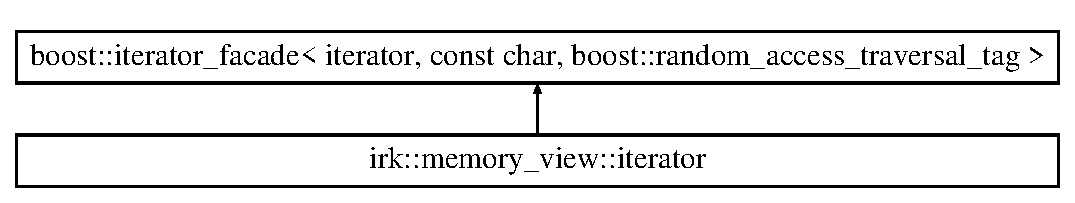
\includegraphics[height=2.000000cm]{classirk_1_1memory__view_1_1iterator}
\end{center}
\end{figure}
\subsection*{Public Member Functions}
\begin{DoxyCompactItemize}
\item 
\mbox{\hyperlink{classirk_1_1memory__view_1_1iterator_a0844f570d5e10b2d0cc766d7ccb85ed1}{iterator}} ()=default
\item 
\mbox{\hyperlink{classirk_1_1memory__view_1_1iterator_adfc32ee12fc8dad6ede91a5def7b37fd}{iterator}} (const char $\ast$pos)
\end{DoxyCompactItemize}
\subsection*{Friends}
\begin{DoxyCompactItemize}
\item 
class \mbox{\hyperlink{classirk_1_1memory__view_1_1iterator_ac09f73e325921cc50ebcd96bed0f8096}{boost\+::iterator\+\_\+core\+\_\+access}}
\end{DoxyCompactItemize}


\subsection{Detailed Description}
Character iterator. 

\subsection{Constructor \& Destructor Documentation}
\mbox{\Hypertarget{classirk_1_1memory__view_1_1iterator_a0844f570d5e10b2d0cc766d7ccb85ed1}\label{classirk_1_1memory__view_1_1iterator_a0844f570d5e10b2d0cc766d7ccb85ed1}} 
\index{irk\+::memory\+\_\+view\+::iterator@{irk\+::memory\+\_\+view\+::iterator}!iterator@{iterator}}
\index{iterator@{iterator}!irk\+::memory\+\_\+view\+::iterator@{irk\+::memory\+\_\+view\+::iterator}}
\subsubsection{\texorpdfstring{iterator()}{iterator()}\hspace{0.1cm}{\footnotesize\ttfamily [1/2]}}
{\footnotesize\ttfamily irk\+::memory\+\_\+view\+::iterator\+::iterator (\begin{DoxyParamCaption}{ }\end{DoxyParamCaption})\hspace{0.3cm}{\ttfamily [default]}}

\mbox{\Hypertarget{classirk_1_1memory__view_1_1iterator_adfc32ee12fc8dad6ede91a5def7b37fd}\label{classirk_1_1memory__view_1_1iterator_adfc32ee12fc8dad6ede91a5def7b37fd}} 
\index{irk\+::memory\+\_\+view\+::iterator@{irk\+::memory\+\_\+view\+::iterator}!iterator@{iterator}}
\index{iterator@{iterator}!irk\+::memory\+\_\+view\+::iterator@{irk\+::memory\+\_\+view\+::iterator}}
\subsubsection{\texorpdfstring{iterator()}{iterator()}\hspace{0.1cm}{\footnotesize\ttfamily [2/2]}}
{\footnotesize\ttfamily irk\+::memory\+\_\+view\+::iterator\+::iterator (\begin{DoxyParamCaption}\item[{const char $\ast$}]{pos }\end{DoxyParamCaption})\hspace{0.3cm}{\ttfamily [inline]}}



\subsection{Friends And Related Function Documentation}
\mbox{\Hypertarget{classirk_1_1memory__view_1_1iterator_ac09f73e325921cc50ebcd96bed0f8096}\label{classirk_1_1memory__view_1_1iterator_ac09f73e325921cc50ebcd96bed0f8096}} 
\index{irk\+::memory\+\_\+view\+::iterator@{irk\+::memory\+\_\+view\+::iterator}!boost\+::iterator\+\_\+core\+\_\+access@{boost\+::iterator\+\_\+core\+\_\+access}}
\index{boost\+::iterator\+\_\+core\+\_\+access@{boost\+::iterator\+\_\+core\+\_\+access}!irk\+::memory\+\_\+view\+::iterator@{irk\+::memory\+\_\+view\+::iterator}}
\subsubsection{\texorpdfstring{boost\+::iterator\+\_\+core\+\_\+access}{boost::iterator\_core\_access}}
{\footnotesize\ttfamily friend class boost\+::iterator\+\_\+core\+\_\+access\hspace{0.3cm}{\ttfamily [friend]}}



The documentation for this class was generated from the following file\+:\begin{DoxyCompactItemize}
\item 
include/irkit/\mbox{\hyperlink{memoryview_8hpp}{memoryview.\+hpp}}\end{DoxyCompactItemize}

\hypertarget{classirk_1_1index_1_1zipped__payload__list__view_1_1iterator}{}\section{irk\+:\+:index\+:\+:zipped\+\_\+payload\+\_\+list\+\_\+view$<$ Payload $>$\+:\+:iterator Class Reference}
\label{classirk_1_1index_1_1zipped__payload__list__view_1_1iterator}\index{irk\+::index\+::zipped\+\_\+payload\+\_\+list\+\_\+view$<$ Payload $>$\+::iterator@{irk\+::index\+::zipped\+\_\+payload\+\_\+list\+\_\+view$<$ Payload $>$\+::iterator}}


{\ttfamily \#include $<$block\+\_\+inverted\+\_\+list.\+hpp$>$}

Inheritance diagram for irk\+:\+:index\+:\+:zipped\+\_\+payload\+\_\+list\+\_\+view$<$ Payload $>$\+:\+:iterator\+:\begin{figure}[H]
\begin{center}
\leavevmode
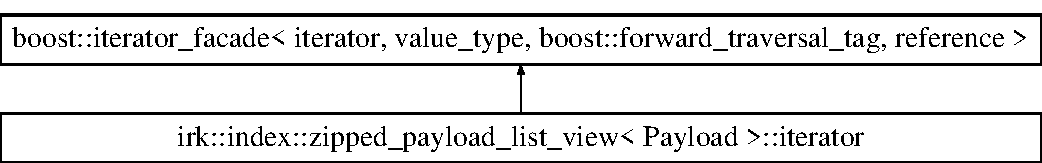
\includegraphics[height=2.000000cm]{classirk_1_1index_1_1zipped__payload__list__view_1_1iterator}
\end{center}
\end{figure}
\subsection*{Public Member Functions}
\begin{DoxyCompactItemize}
\item 
\mbox{\hyperlink{classirk_1_1index_1_1zipped__payload__list__view_1_1iterator_a469993754f092a3996e4de3c61411faf}{iterator}} (typename \mbox{\hyperlink{classirk_1_1index_1_1block__payload__list__view}{block\+\_\+payload\+\_\+list\+\_\+view}}$<$ Payload $>$\+::iterator... iterators)
\item 
{\footnotesize template$<$class Block\+Iterator , std\+::size\+\_\+t... I$>$ }\\\mbox{\hyperlink{classirk_1_1index_1_1zipped__payload__list__view_1_1iterator}{iterator}} \& \mbox{\hyperlink{classirk_1_1index_1_1zipped__payload__list__view_1_1iterator_a66e4e30f467ffca4b6b4328d55bf7f60}{align}} (const Block\+Iterator \&other, std\+::index\+\_\+sequence$<$ I... $>$)
\item 
{\footnotesize template$<$class Block\+Iterator $>$ }\\\mbox{\hyperlink{classirk_1_1index_1_1zipped__payload__list__view_1_1iterator}{iterator}} \& \mbox{\hyperlink{classirk_1_1index_1_1zipped__payload__list__view_1_1iterator_a5b941810905eb53ba4d1a0ee5a7b501a}{align}} (const Block\+Iterator \&other)
\item 
{\footnotesize template$<$std\+::size\+\_\+t idx$>$ }\\auto \mbox{\hyperlink{classirk_1_1index_1_1zipped__payload__list__view_1_1iterator_afb5b7b389b5952ff0bdb5eb6e90ea3cd}{payload}} () const
\end{DoxyCompactItemize}
\subsection*{Friends}
\begin{DoxyCompactItemize}
\item 
class \mbox{\hyperlink{classirk_1_1index_1_1zipped__payload__list__view_1_1iterator_ac09f73e325921cc50ebcd96bed0f8096}{boost\+::iterator\+\_\+core\+\_\+access}}
\end{DoxyCompactItemize}


\subsection{Constructor \& Destructor Documentation}
\mbox{\Hypertarget{classirk_1_1index_1_1zipped__payload__list__view_1_1iterator_a469993754f092a3996e4de3c61411faf}\label{classirk_1_1index_1_1zipped__payload__list__view_1_1iterator_a469993754f092a3996e4de3c61411faf}} 
\index{irk\+::index\+::zipped\+\_\+payload\+\_\+list\+\_\+view\+::iterator@{irk\+::index\+::zipped\+\_\+payload\+\_\+list\+\_\+view\+::iterator}!iterator@{iterator}}
\index{iterator@{iterator}!irk\+::index\+::zipped\+\_\+payload\+\_\+list\+\_\+view\+::iterator@{irk\+::index\+::zipped\+\_\+payload\+\_\+list\+\_\+view\+::iterator}}
\subsubsection{\texorpdfstring{iterator()}{iterator()}}
{\footnotesize\ttfamily template$<$class ... Payload$>$ \\
\mbox{\hyperlink{classirk_1_1index_1_1zipped__payload__list__view}{irk\+::index\+::zipped\+\_\+payload\+\_\+list\+\_\+view}}$<$ Payload $>$\+::iterator\+::iterator (\begin{DoxyParamCaption}\item[{typename \mbox{\hyperlink{classirk_1_1index_1_1block__payload__list__view}{block\+\_\+payload\+\_\+list\+\_\+view}}$<$ Payload $>$\+::iterator...}]{iterators }\end{DoxyParamCaption})\hspace{0.3cm}{\ttfamily [inline]}}



\subsection{Member Function Documentation}
\mbox{\Hypertarget{classirk_1_1index_1_1zipped__payload__list__view_1_1iterator_a66e4e30f467ffca4b6b4328d55bf7f60}\label{classirk_1_1index_1_1zipped__payload__list__view_1_1iterator_a66e4e30f467ffca4b6b4328d55bf7f60}} 
\index{irk\+::index\+::zipped\+\_\+payload\+\_\+list\+\_\+view\+::iterator@{irk\+::index\+::zipped\+\_\+payload\+\_\+list\+\_\+view\+::iterator}!align@{align}}
\index{align@{align}!irk\+::index\+::zipped\+\_\+payload\+\_\+list\+\_\+view\+::iterator@{irk\+::index\+::zipped\+\_\+payload\+\_\+list\+\_\+view\+::iterator}}
\subsubsection{\texorpdfstring{align()}{align()}\hspace{0.1cm}{\footnotesize\ttfamily [1/2]}}
{\footnotesize\ttfamily template$<$class ... Payload$>$ \\
template$<$class Block\+Iterator , std\+::size\+\_\+t... I$>$ \\
\mbox{\hyperlink{classirk_1_1index_1_1zipped__payload__list__view_1_1iterator}{iterator}}\& \mbox{\hyperlink{classirk_1_1index_1_1zipped__payload__list__view}{irk\+::index\+::zipped\+\_\+payload\+\_\+list\+\_\+view}}$<$ Payload $>$\+::iterator\+::align (\begin{DoxyParamCaption}\item[{const Block\+Iterator \&}]{other,  }\item[{std\+::index\+\_\+sequence$<$ I... $>$}]{ }\end{DoxyParamCaption})\hspace{0.3cm}{\ttfamily [inline]}}

\mbox{\Hypertarget{classirk_1_1index_1_1zipped__payload__list__view_1_1iterator_a5b941810905eb53ba4d1a0ee5a7b501a}\label{classirk_1_1index_1_1zipped__payload__list__view_1_1iterator_a5b941810905eb53ba4d1a0ee5a7b501a}} 
\index{irk\+::index\+::zipped\+\_\+payload\+\_\+list\+\_\+view\+::iterator@{irk\+::index\+::zipped\+\_\+payload\+\_\+list\+\_\+view\+::iterator}!align@{align}}
\index{align@{align}!irk\+::index\+::zipped\+\_\+payload\+\_\+list\+\_\+view\+::iterator@{irk\+::index\+::zipped\+\_\+payload\+\_\+list\+\_\+view\+::iterator}}
\subsubsection{\texorpdfstring{align()}{align()}\hspace{0.1cm}{\footnotesize\ttfamily [2/2]}}
{\footnotesize\ttfamily template$<$class ... Payload$>$ \\
template$<$class Block\+Iterator $>$ \\
\mbox{\hyperlink{classirk_1_1index_1_1zipped__payload__list__view_1_1iterator}{iterator}}\& \mbox{\hyperlink{classirk_1_1index_1_1zipped__payload__list__view}{irk\+::index\+::zipped\+\_\+payload\+\_\+list\+\_\+view}}$<$ Payload $>$\+::iterator\+::align (\begin{DoxyParamCaption}\item[{const Block\+Iterator \&}]{other }\end{DoxyParamCaption})\hspace{0.3cm}{\ttfamily [inline]}}

\mbox{\Hypertarget{classirk_1_1index_1_1zipped__payload__list__view_1_1iterator_afb5b7b389b5952ff0bdb5eb6e90ea3cd}\label{classirk_1_1index_1_1zipped__payload__list__view_1_1iterator_afb5b7b389b5952ff0bdb5eb6e90ea3cd}} 
\index{irk\+::index\+::zipped\+\_\+payload\+\_\+list\+\_\+view\+::iterator@{irk\+::index\+::zipped\+\_\+payload\+\_\+list\+\_\+view\+::iterator}!payload@{payload}}
\index{payload@{payload}!irk\+::index\+::zipped\+\_\+payload\+\_\+list\+\_\+view\+::iterator@{irk\+::index\+::zipped\+\_\+payload\+\_\+list\+\_\+view\+::iterator}}
\subsubsection{\texorpdfstring{payload()}{payload()}}
{\footnotesize\ttfamily template$<$class ... Payload$>$ \\
template$<$std\+::size\+\_\+t idx$>$ \\
auto \mbox{\hyperlink{classirk_1_1index_1_1zipped__payload__list__view}{irk\+::index\+::zipped\+\_\+payload\+\_\+list\+\_\+view}}$<$ Payload $>$\+::iterator\+::payload (\begin{DoxyParamCaption}{ }\end{DoxyParamCaption}) const\hspace{0.3cm}{\ttfamily [inline]}}



\subsection{Friends And Related Function Documentation}
\mbox{\Hypertarget{classirk_1_1index_1_1zipped__payload__list__view_1_1iterator_ac09f73e325921cc50ebcd96bed0f8096}\label{classirk_1_1index_1_1zipped__payload__list__view_1_1iterator_ac09f73e325921cc50ebcd96bed0f8096}} 
\index{irk\+::index\+::zipped\+\_\+payload\+\_\+list\+\_\+view\+::iterator@{irk\+::index\+::zipped\+\_\+payload\+\_\+list\+\_\+view\+::iterator}!boost\+::iterator\+\_\+core\+\_\+access@{boost\+::iterator\+\_\+core\+\_\+access}}
\index{boost\+::iterator\+\_\+core\+\_\+access@{boost\+::iterator\+\_\+core\+\_\+access}!irk\+::index\+::zipped\+\_\+payload\+\_\+list\+\_\+view\+::iterator@{irk\+::index\+::zipped\+\_\+payload\+\_\+list\+\_\+view\+::iterator}}
\subsubsection{\texorpdfstring{boost\+::iterator\+\_\+core\+\_\+access}{boost::iterator\_core\_access}}
{\footnotesize\ttfamily template$<$class ... Payload$>$ \\
friend class boost\+::iterator\+\_\+core\+\_\+access\hspace{0.3cm}{\ttfamily [friend]}}



The documentation for this class was generated from the following file\+:\begin{DoxyCompactItemize}
\item 
include/irkit/index/\mbox{\hyperlink{block__inverted__list_8hpp}{block\+\_\+inverted\+\_\+list.\+hpp}}\end{DoxyCompactItemize}

\hypertarget{classirk_1_1index_1_1block__posting__list__view_1_1iterator}{}\section{irk\+:\+:index\+:\+:block\+\_\+posting\+\_\+list\+\_\+view$<$ Doc, Payload $>$\+:\+:iterator$<$ payload\+\_\+type $>$ Class Template Reference}
\label{classirk_1_1index_1_1block__posting__list__view_1_1iterator}\index{irk\+::index\+::block\+\_\+posting\+\_\+list\+\_\+view$<$ Doc, Payload $>$\+::iterator$<$ payload\+\_\+type $>$@{irk\+::index\+::block\+\_\+posting\+\_\+list\+\_\+view$<$ Doc, Payload $>$\+::iterator$<$ payload\+\_\+type $>$}}


Document iterator.  




{\ttfamily \#include $<$block\+\_\+inverted\+\_\+list.\+hpp$>$}

Inheritance diagram for irk\+:\+:index\+:\+:block\+\_\+posting\+\_\+list\+\_\+view$<$ Doc, Payload $>$\+:\+:iterator$<$ payload\+\_\+type $>$\+:\begin{figure}[H]
\begin{center}
\leavevmode
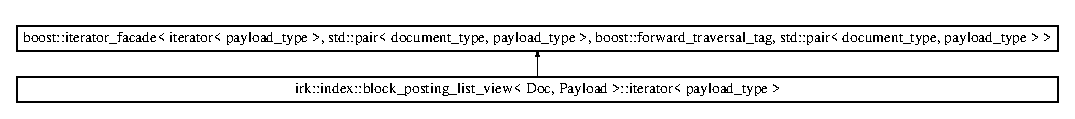
\includegraphics[height=1.154639cm]{classirk_1_1index_1_1block__posting__list__view_1_1iterator}
\end{center}
\end{figure}
\subsection*{Public Member Functions}
\begin{DoxyCompactItemize}
\item 
\mbox{\hyperlink{classirk_1_1index_1_1block__posting__list__view_1_1iterator_a72038769859b9c21965abab4736e1e9c}{iterator}} (\mbox{\hyperlink{classirk_1_1index_1_1block__posting__list__view_a5b6c3f910a1bd819ff3efa0a619e32a0}{document\+\_\+iterator\+\_\+t}} document\+\_\+iterator, \mbox{\hyperlink{classirk_1_1index_1_1block__posting__list__view_ad7beed21d25c7cb3b2b389c28022be12}{payload\+\_\+iterator\+\_\+t}} payload\+\_\+iterator)
\item 
\mbox{\hyperlink{classirk_1_1index_1_1block__posting__list__view_1_1iterator}{iterator}} \& \mbox{\hyperlink{classirk_1_1index_1_1block__posting__list__view_1_1iterator_a35c46c592f4f06ae24945bf6881efc2a}{moveto}} (\mbox{\hyperlink{classirk_1_1index_1_1block__posting__list__view_a4a778116d22c9cf347f38da132ca0900}{document\+\_\+type}} doc)
\item 
\mbox{\hyperlink{classirk_1_1index_1_1block__posting__list__view_1_1iterator}{iterator}} \mbox{\hyperlink{classirk_1_1index_1_1block__posting__list__view_1_1iterator_ab330da1b4a727e2afadb5469fc80e4f0}{nextgeq}} (\mbox{\hyperlink{classirk_1_1index_1_1block__posting__list__view_a4a778116d22c9cf347f38da132ca0900}{document\+\_\+type}} doc)
\item 
const \mbox{\hyperlink{classirk_1_1index_1_1block__posting__list__view_a4a778116d22c9cf347f38da132ca0900}{document\+\_\+type}} \& \mbox{\hyperlink{classirk_1_1index_1_1block__posting__list__view_1_1iterator_a6dfbadd2661f2f37723800b4acc7c7ce}{document}} () const
\item 
payload\+\_\+type \mbox{\hyperlink{classirk_1_1index_1_1block__posting__list__view_1_1iterator_a8bf0051cfe9dfef27c3a7a627ad51987}{payload}} () const
\end{DoxyCompactItemize}
\subsection*{Friends}
\begin{DoxyCompactItemize}
\item 
class \mbox{\hyperlink{classirk_1_1index_1_1block__posting__list__view_1_1iterator_ac09f73e325921cc50ebcd96bed0f8096}{boost\+::iterator\+\_\+core\+\_\+access}}
\end{DoxyCompactItemize}


\subsection{Detailed Description}
\subsubsection*{template$<$class Doc, class... Payload$>$\newline
template$<$class payload\+\_\+type$>$\newline
class irk\+::index\+::block\+\_\+posting\+\_\+list\+\_\+view$<$ Doc, Payload $>$\+::iterator$<$ payload\+\_\+type $>$}

Document iterator. 

\subsection{Constructor \& Destructor Documentation}
\mbox{\Hypertarget{classirk_1_1index_1_1block__posting__list__view_1_1iterator_a72038769859b9c21965abab4736e1e9c}\label{classirk_1_1index_1_1block__posting__list__view_1_1iterator_a72038769859b9c21965abab4736e1e9c}} 
\index{irk\+::index\+::block\+\_\+posting\+\_\+list\+\_\+view\+::iterator@{irk\+::index\+::block\+\_\+posting\+\_\+list\+\_\+view\+::iterator}!iterator@{iterator}}
\index{iterator@{iterator}!irk\+::index\+::block\+\_\+posting\+\_\+list\+\_\+view\+::iterator@{irk\+::index\+::block\+\_\+posting\+\_\+list\+\_\+view\+::iterator}}
\subsubsection{\texorpdfstring{iterator()}{iterator()}}
{\footnotesize\ttfamily template$<$class Doc , class... Payload$>$ \\
template$<$class payload\+\_\+type $>$ \\
\mbox{\hyperlink{classirk_1_1index_1_1block__posting__list__view}{irk\+::index\+::block\+\_\+posting\+\_\+list\+\_\+view}}$<$ Doc, Payload $>$\+::\mbox{\hyperlink{classirk_1_1index_1_1block__posting__list__view_1_1iterator}{iterator}}$<$ payload\+\_\+type $>$\+::\mbox{\hyperlink{classirk_1_1index_1_1block__posting__list__view_1_1iterator}{iterator}} (\begin{DoxyParamCaption}\item[{\mbox{\hyperlink{classirk_1_1index_1_1block__posting__list__view_a5b6c3f910a1bd819ff3efa0a619e32a0}{document\+\_\+iterator\+\_\+t}}}]{document\+\_\+iterator,  }\item[{\mbox{\hyperlink{classirk_1_1index_1_1block__posting__list__view_ad7beed21d25c7cb3b2b389c28022be12}{payload\+\_\+iterator\+\_\+t}}}]{payload\+\_\+iterator }\end{DoxyParamCaption})\hspace{0.3cm}{\ttfamily [inline]}}



\subsection{Member Function Documentation}
\mbox{\Hypertarget{classirk_1_1index_1_1block__posting__list__view_1_1iterator_a6dfbadd2661f2f37723800b4acc7c7ce}\label{classirk_1_1index_1_1block__posting__list__view_1_1iterator_a6dfbadd2661f2f37723800b4acc7c7ce}} 
\index{irk\+::index\+::block\+\_\+posting\+\_\+list\+\_\+view\+::iterator@{irk\+::index\+::block\+\_\+posting\+\_\+list\+\_\+view\+::iterator}!document@{document}}
\index{document@{document}!irk\+::index\+::block\+\_\+posting\+\_\+list\+\_\+view\+::iterator@{irk\+::index\+::block\+\_\+posting\+\_\+list\+\_\+view\+::iterator}}
\subsubsection{\texorpdfstring{document()}{document()}}
{\footnotesize\ttfamily template$<$class Doc , class... Payload$>$ \\
template$<$class payload\+\_\+type $>$ \\
const \mbox{\hyperlink{classirk_1_1index_1_1block__posting__list__view_a4a778116d22c9cf347f38da132ca0900}{document\+\_\+type}}\& \mbox{\hyperlink{classirk_1_1index_1_1block__posting__list__view}{irk\+::index\+::block\+\_\+posting\+\_\+list\+\_\+view}}$<$ Doc, Payload $>$\+::\mbox{\hyperlink{classirk_1_1index_1_1block__posting__list__view_1_1iterator}{iterator}}$<$ payload\+\_\+type $>$\+::document (\begin{DoxyParamCaption}{ }\end{DoxyParamCaption}) const\hspace{0.3cm}{\ttfamily [inline]}}

\mbox{\Hypertarget{classirk_1_1index_1_1block__posting__list__view_1_1iterator_a35c46c592f4f06ae24945bf6881efc2a}\label{classirk_1_1index_1_1block__posting__list__view_1_1iterator_a35c46c592f4f06ae24945bf6881efc2a}} 
\index{irk\+::index\+::block\+\_\+posting\+\_\+list\+\_\+view\+::iterator@{irk\+::index\+::block\+\_\+posting\+\_\+list\+\_\+view\+::iterator}!moveto@{moveto}}
\index{moveto@{moveto}!irk\+::index\+::block\+\_\+posting\+\_\+list\+\_\+view\+::iterator@{irk\+::index\+::block\+\_\+posting\+\_\+list\+\_\+view\+::iterator}}
\subsubsection{\texorpdfstring{moveto()}{moveto()}}
{\footnotesize\ttfamily template$<$class Doc , class... Payload$>$ \\
template$<$class payload\+\_\+type $>$ \\
\mbox{\hyperlink{classirk_1_1index_1_1block__posting__list__view_1_1iterator}{iterator}}\& \mbox{\hyperlink{classirk_1_1index_1_1block__posting__list__view}{irk\+::index\+::block\+\_\+posting\+\_\+list\+\_\+view}}$<$ Doc, Payload $>$\+::\mbox{\hyperlink{classirk_1_1index_1_1block__posting__list__view_1_1iterator}{iterator}}$<$ payload\+\_\+type $>$\+::moveto (\begin{DoxyParamCaption}\item[{\mbox{\hyperlink{classirk_1_1index_1_1block__posting__list__view_a4a778116d22c9cf347f38da132ca0900}{document\+\_\+type}}}]{doc }\end{DoxyParamCaption})\hspace{0.3cm}{\ttfamily [inline]}}

\mbox{\Hypertarget{classirk_1_1index_1_1block__posting__list__view_1_1iterator_ab330da1b4a727e2afadb5469fc80e4f0}\label{classirk_1_1index_1_1block__posting__list__view_1_1iterator_ab330da1b4a727e2afadb5469fc80e4f0}} 
\index{irk\+::index\+::block\+\_\+posting\+\_\+list\+\_\+view\+::iterator@{irk\+::index\+::block\+\_\+posting\+\_\+list\+\_\+view\+::iterator}!nextgeq@{nextgeq}}
\index{nextgeq@{nextgeq}!irk\+::index\+::block\+\_\+posting\+\_\+list\+\_\+view\+::iterator@{irk\+::index\+::block\+\_\+posting\+\_\+list\+\_\+view\+::iterator}}
\subsubsection{\texorpdfstring{nextgeq()}{nextgeq()}}
{\footnotesize\ttfamily template$<$class Doc , class... Payload$>$ \\
template$<$class payload\+\_\+type $>$ \\
\mbox{\hyperlink{classirk_1_1index_1_1block__posting__list__view_1_1iterator}{iterator}} \mbox{\hyperlink{classirk_1_1index_1_1block__posting__list__view}{irk\+::index\+::block\+\_\+posting\+\_\+list\+\_\+view}}$<$ Doc, Payload $>$\+::\mbox{\hyperlink{classirk_1_1index_1_1block__posting__list__view_1_1iterator}{iterator}}$<$ payload\+\_\+type $>$\+::nextgeq (\begin{DoxyParamCaption}\item[{\mbox{\hyperlink{classirk_1_1index_1_1block__posting__list__view_a4a778116d22c9cf347f38da132ca0900}{document\+\_\+type}}}]{doc }\end{DoxyParamCaption})\hspace{0.3cm}{\ttfamily [inline]}}

\mbox{\Hypertarget{classirk_1_1index_1_1block__posting__list__view_1_1iterator_a8bf0051cfe9dfef27c3a7a627ad51987}\label{classirk_1_1index_1_1block__posting__list__view_1_1iterator_a8bf0051cfe9dfef27c3a7a627ad51987}} 
\index{irk\+::index\+::block\+\_\+posting\+\_\+list\+\_\+view\+::iterator@{irk\+::index\+::block\+\_\+posting\+\_\+list\+\_\+view\+::iterator}!payload@{payload}}
\index{payload@{payload}!irk\+::index\+::block\+\_\+posting\+\_\+list\+\_\+view\+::iterator@{irk\+::index\+::block\+\_\+posting\+\_\+list\+\_\+view\+::iterator}}
\subsubsection{\texorpdfstring{payload()}{payload()}}
{\footnotesize\ttfamily template$<$class Doc , class... Payload$>$ \\
template$<$class payload\+\_\+type $>$ \\
payload\+\_\+type \mbox{\hyperlink{classirk_1_1index_1_1block__posting__list__view}{irk\+::index\+::block\+\_\+posting\+\_\+list\+\_\+view}}$<$ Doc, Payload $>$\+::\mbox{\hyperlink{classirk_1_1index_1_1block__posting__list__view_1_1iterator}{iterator}}$<$ payload\+\_\+type $>$\+::payload (\begin{DoxyParamCaption}{ }\end{DoxyParamCaption}) const\hspace{0.3cm}{\ttfamily [inline]}}



\subsection{Friends And Related Function Documentation}
\mbox{\Hypertarget{classirk_1_1index_1_1block__posting__list__view_1_1iterator_ac09f73e325921cc50ebcd96bed0f8096}\label{classirk_1_1index_1_1block__posting__list__view_1_1iterator_ac09f73e325921cc50ebcd96bed0f8096}} 
\index{irk\+::index\+::block\+\_\+posting\+\_\+list\+\_\+view\+::iterator@{irk\+::index\+::block\+\_\+posting\+\_\+list\+\_\+view\+::iterator}!boost\+::iterator\+\_\+core\+\_\+access@{boost\+::iterator\+\_\+core\+\_\+access}}
\index{boost\+::iterator\+\_\+core\+\_\+access@{boost\+::iterator\+\_\+core\+\_\+access}!irk\+::index\+::block\+\_\+posting\+\_\+list\+\_\+view\+::iterator@{irk\+::index\+::block\+\_\+posting\+\_\+list\+\_\+view\+::iterator}}
\subsubsection{\texorpdfstring{boost\+::iterator\+\_\+core\+\_\+access}{boost::iterator\_core\_access}}
{\footnotesize\ttfamily template$<$class Doc , class... Payload$>$ \\
template$<$class payload\+\_\+type $>$ \\
friend class boost\+::iterator\+\_\+core\+\_\+access\hspace{0.3cm}{\ttfamily [friend]}}



The documentation for this class was generated from the following file\+:\begin{DoxyCompactItemize}
\item 
include/irkit/index/\mbox{\hyperlink{block__inverted__list_8hpp}{block\+\_\+inverted\+\_\+list.\+hpp}}\end{DoxyCompactItemize}

\hypertarget{classirk_1_1prefix__map_1_1iterator}{}\section{irk\+:\+:prefix\+\_\+map$<$ Index, Memory\+Buffer, Counter $>$\+:\+:iterator Class Reference}
\label{classirk_1_1prefix__map_1_1iterator}\index{irk\+::prefix\+\_\+map$<$ Index, Memory\+Buffer, Counter $>$\+::iterator@{irk\+::prefix\+\_\+map$<$ Index, Memory\+Buffer, Counter $>$\+::iterator}}


{\ttfamily \#include $<$prefixmap.\+hpp$>$}

Inheritance diagram for irk\+:\+:prefix\+\_\+map$<$ Index, Memory\+Buffer, Counter $>$\+:\+:iterator\+:\begin{figure}[H]
\begin{center}
\leavevmode
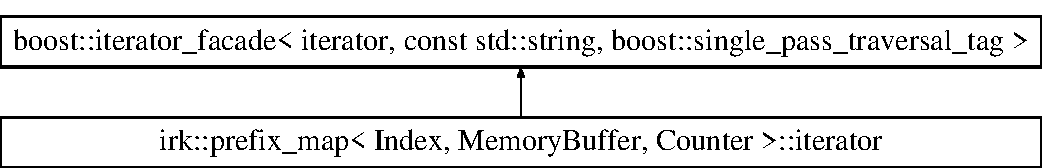
\includegraphics[height=2.000000cm]{classirk_1_1prefix__map_1_1iterator}
\end{center}
\end{figure}
\subsection*{Public Member Functions}
\begin{DoxyCompactItemize}
\item 
\mbox{\hyperlink{classirk_1_1prefix__map_1_1iterator_a5701dce183a096eb3c55cfd3d52c803b}{iterator}} (const Memory\+Buffer \&blocks, int block\+\_\+size, \mbox{\hyperlink{classirk_1_1prefix__map_1_1block__ptr}{block\+\_\+ptr}} block, int block\+\_\+num, int pos\+\_\+in\+\_\+block, const std\+::shared\+\_\+ptr$<$ \mbox{\hyperlink{classirk_1_1hutucker__codec}{hutucker\+\_\+codec}}$<$ char $>$$>$ codec)
\end{DoxyCompactItemize}
\subsection*{Friends}
\begin{DoxyCompactItemize}
\item 
class \mbox{\hyperlink{classirk_1_1prefix__map_1_1iterator_ac09f73e325921cc50ebcd96bed0f8096}{boost\+::iterator\+\_\+core\+\_\+access}}
\end{DoxyCompactItemize}


\subsection{Constructor \& Destructor Documentation}
\mbox{\Hypertarget{classirk_1_1prefix__map_1_1iterator_a5701dce183a096eb3c55cfd3d52c803b}\label{classirk_1_1prefix__map_1_1iterator_a5701dce183a096eb3c55cfd3d52c803b}} 
\index{irk\+::prefix\+\_\+map\+::iterator@{irk\+::prefix\+\_\+map\+::iterator}!iterator@{iterator}}
\index{iterator@{iterator}!irk\+::prefix\+\_\+map\+::iterator@{irk\+::prefix\+\_\+map\+::iterator}}
\subsubsection{\texorpdfstring{iterator()}{iterator()}}
{\footnotesize\ttfamily template$<$class Index, class Memory\+Buffer, class Counter = std\+::uint32\+\_\+t$>$ \\
\mbox{\hyperlink{classirk_1_1prefix__map}{irk\+::prefix\+\_\+map}}$<$ Index, Memory\+Buffer, Counter $>$\+::iterator\+::iterator (\begin{DoxyParamCaption}\item[{const Memory\+Buffer \&}]{blocks,  }\item[{int}]{block\+\_\+size,  }\item[{\mbox{\hyperlink{classirk_1_1prefix__map_1_1block__ptr}{block\+\_\+ptr}}}]{block,  }\item[{int}]{block\+\_\+num,  }\item[{int}]{pos\+\_\+in\+\_\+block,  }\item[{const std\+::shared\+\_\+ptr$<$ \mbox{\hyperlink{classirk_1_1hutucker__codec}{hutucker\+\_\+codec}}$<$ char $>$$>$}]{codec }\end{DoxyParamCaption})\hspace{0.3cm}{\ttfamily [inline]}}



\subsection{Friends And Related Function Documentation}
\mbox{\Hypertarget{classirk_1_1prefix__map_1_1iterator_ac09f73e325921cc50ebcd96bed0f8096}\label{classirk_1_1prefix__map_1_1iterator_ac09f73e325921cc50ebcd96bed0f8096}} 
\index{irk\+::prefix\+\_\+map\+::iterator@{irk\+::prefix\+\_\+map\+::iterator}!boost\+::iterator\+\_\+core\+\_\+access@{boost\+::iterator\+\_\+core\+\_\+access}}
\index{boost\+::iterator\+\_\+core\+\_\+access@{boost\+::iterator\+\_\+core\+\_\+access}!irk\+::prefix\+\_\+map\+::iterator@{irk\+::prefix\+\_\+map\+::iterator}}
\subsubsection{\texorpdfstring{boost\+::iterator\+\_\+core\+\_\+access}{boost::iterator\_core\_access}}
{\footnotesize\ttfamily template$<$class Index, class Memory\+Buffer, class Counter = std\+::uint32\+\_\+t$>$ \\
friend class boost\+::iterator\+\_\+core\+\_\+access\hspace{0.3cm}{\ttfamily [friend]}}



The documentation for this class was generated from the following file\+:\begin{DoxyCompactItemize}
\item 
include/irkit/\mbox{\hyperlink{prefixmap_8hpp}{prefixmap.\+hpp}}\end{DoxyCompactItemize}

\hypertarget{classirk_1_1posting__list__view_1_1iterator}{}\section{irk\+:\+:posting\+\_\+list\+\_\+view$<$ Document\+ListT, Payload\+ListT $>$\+:\+:iterator Class Reference}
\label{classirk_1_1posting__list__view_1_1iterator}\index{irk\+::posting\+\_\+list\+\_\+view$<$ Document\+List\+T, Payload\+List\+T $>$\+::iterator@{irk\+::posting\+\_\+list\+\_\+view$<$ Document\+List\+T, Payload\+List\+T $>$\+::iterator}}


{\ttfamily \#include $<$posting\+\_\+list.\+hpp$>$}

Inheritance diagram for irk\+:\+:posting\+\_\+list\+\_\+view$<$ Document\+ListT, Payload\+ListT $>$\+:\+:iterator\+:\begin{figure}[H]
\begin{center}
\leavevmode
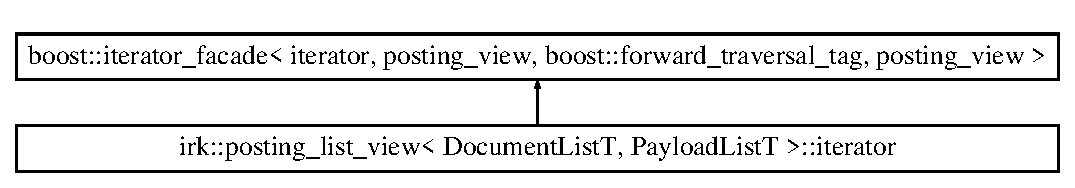
\includegraphics[height=2.000000cm]{classirk_1_1posting__list__view_1_1iterator}
\end{center}
\end{figure}
\subsection*{Public Member Functions}
\begin{DoxyCompactItemize}
\item 
\mbox{\hyperlink{classirk_1_1posting__list__view_1_1iterator_a0735df34097a1113f0295d27791f985d}{iterator}} (\mbox{\hyperlink{classirk_1_1posting__list__view_abaca622760e6da2c67d55cf35207250f}{document\+\_\+iterator\+\_\+t}} document\+\_\+iterator, \mbox{\hyperlink{classirk_1_1posting__list__view_a5a153169348a164ea2cb1a18dc76e279}{payload\+\_\+iterator\+\_\+t}} payload\+\_\+iterator)
\item 
\mbox{\hyperlink{classirk_1_1posting__list__view_1_1iterator_aa4053b60f98871ed18bf6bfb87dfdd18}{iterator}} (const \mbox{\hyperlink{classirk_1_1posting__list__view_1_1iterator}{iterator}} \&other)
\item 
\mbox{\hyperlink{classirk_1_1posting__list__view_1_1iterator}{iterator}} \& \mbox{\hyperlink{classirk_1_1posting__list__view_1_1iterator_a2f70673e696d84d36854a359b749cd49}{moveto}} (\mbox{\hyperlink{classirk_1_1posting__list__view_ac4615e6e3d8ee1eb9a847b7a34919977}{document\+\_\+type}} doc)
\item 
\mbox{\hyperlink{classirk_1_1posting__list__view_1_1iterator}{iterator}} \mbox{\hyperlink{classirk_1_1posting__list__view_1_1iterator_ac86c0cfbfa10ffc60fcde9a1af51bbc3}{nextgeq}} (\mbox{\hyperlink{classirk_1_1posting__list__view_ac4615e6e3d8ee1eb9a847b7a34919977}{document\+\_\+type}} doc) const
\end{DoxyCompactItemize}
\subsection*{Friends}
\begin{DoxyCompactItemize}
\item 
class \mbox{\hyperlink{classirk_1_1posting__list__view_1_1iterator_ac09f73e325921cc50ebcd96bed0f8096}{boost\+::iterator\+\_\+core\+\_\+access}}
\end{DoxyCompactItemize}


\subsection{Constructor \& Destructor Documentation}
\mbox{\Hypertarget{classirk_1_1posting__list__view_1_1iterator_a0735df34097a1113f0295d27791f985d}\label{classirk_1_1posting__list__view_1_1iterator_a0735df34097a1113f0295d27791f985d}} 
\index{irk\+::posting\+\_\+list\+\_\+view\+::iterator@{irk\+::posting\+\_\+list\+\_\+view\+::iterator}!iterator@{iterator}}
\index{iterator@{iterator}!irk\+::posting\+\_\+list\+\_\+view\+::iterator@{irk\+::posting\+\_\+list\+\_\+view\+::iterator}}
\subsubsection{\texorpdfstring{iterator()}{iterator()}\hspace{0.1cm}{\footnotesize\ttfamily [1/2]}}
{\footnotesize\ttfamily template$<$class Document\+ListT , class Payload\+ListT $>$ \\
\mbox{\hyperlink{classirk_1_1posting__list__view}{irk\+::posting\+\_\+list\+\_\+view}}$<$ Document\+ListT, Payload\+ListT $>$\+::iterator\+::iterator (\begin{DoxyParamCaption}\item[{\mbox{\hyperlink{classirk_1_1posting__list__view_abaca622760e6da2c67d55cf35207250f}{document\+\_\+iterator\+\_\+t}}}]{document\+\_\+iterator,  }\item[{\mbox{\hyperlink{classirk_1_1posting__list__view_a5a153169348a164ea2cb1a18dc76e279}{payload\+\_\+iterator\+\_\+t}}}]{payload\+\_\+iterator }\end{DoxyParamCaption})\hspace{0.3cm}{\ttfamily [inline]}}

\mbox{\Hypertarget{classirk_1_1posting__list__view_1_1iterator_aa4053b60f98871ed18bf6bfb87dfdd18}\label{classirk_1_1posting__list__view_1_1iterator_aa4053b60f98871ed18bf6bfb87dfdd18}} 
\index{irk\+::posting\+\_\+list\+\_\+view\+::iterator@{irk\+::posting\+\_\+list\+\_\+view\+::iterator}!iterator@{iterator}}
\index{iterator@{iterator}!irk\+::posting\+\_\+list\+\_\+view\+::iterator@{irk\+::posting\+\_\+list\+\_\+view\+::iterator}}
\subsubsection{\texorpdfstring{iterator()}{iterator()}\hspace{0.1cm}{\footnotesize\ttfamily [2/2]}}
{\footnotesize\ttfamily template$<$class Document\+ListT , class Payload\+ListT $>$ \\
\mbox{\hyperlink{classirk_1_1posting__list__view}{irk\+::posting\+\_\+list\+\_\+view}}$<$ Document\+ListT, Payload\+ListT $>$\+::iterator\+::iterator (\begin{DoxyParamCaption}\item[{const \mbox{\hyperlink{classirk_1_1posting__list__view_1_1iterator}{iterator}} \&}]{other }\end{DoxyParamCaption})\hspace{0.3cm}{\ttfamily [inline]}}



\subsection{Member Function Documentation}
\mbox{\Hypertarget{classirk_1_1posting__list__view_1_1iterator_a2f70673e696d84d36854a359b749cd49}\label{classirk_1_1posting__list__view_1_1iterator_a2f70673e696d84d36854a359b749cd49}} 
\index{irk\+::posting\+\_\+list\+\_\+view\+::iterator@{irk\+::posting\+\_\+list\+\_\+view\+::iterator}!moveto@{moveto}}
\index{moveto@{moveto}!irk\+::posting\+\_\+list\+\_\+view\+::iterator@{irk\+::posting\+\_\+list\+\_\+view\+::iterator}}
\subsubsection{\texorpdfstring{moveto()}{moveto()}}
{\footnotesize\ttfamily template$<$class Document\+ListT , class Payload\+ListT $>$ \\
\mbox{\hyperlink{classirk_1_1posting__list__view_1_1iterator}{iterator}}\& \mbox{\hyperlink{classirk_1_1posting__list__view}{irk\+::posting\+\_\+list\+\_\+view}}$<$ Document\+ListT, Payload\+ListT $>$\+::iterator\+::moveto (\begin{DoxyParamCaption}\item[{\mbox{\hyperlink{classirk_1_1posting__list__view_ac4615e6e3d8ee1eb9a847b7a34919977}{document\+\_\+type}}}]{doc }\end{DoxyParamCaption})\hspace{0.3cm}{\ttfamily [inline]}}

\mbox{\Hypertarget{classirk_1_1posting__list__view_1_1iterator_ac86c0cfbfa10ffc60fcde9a1af51bbc3}\label{classirk_1_1posting__list__view_1_1iterator_ac86c0cfbfa10ffc60fcde9a1af51bbc3}} 
\index{irk\+::posting\+\_\+list\+\_\+view\+::iterator@{irk\+::posting\+\_\+list\+\_\+view\+::iterator}!nextgeq@{nextgeq}}
\index{nextgeq@{nextgeq}!irk\+::posting\+\_\+list\+\_\+view\+::iterator@{irk\+::posting\+\_\+list\+\_\+view\+::iterator}}
\subsubsection{\texorpdfstring{nextgeq()}{nextgeq()}}
{\footnotesize\ttfamily template$<$class Document\+ListT , class Payload\+ListT $>$ \\
\mbox{\hyperlink{classirk_1_1posting__list__view_1_1iterator}{iterator}} \mbox{\hyperlink{classirk_1_1posting__list__view}{irk\+::posting\+\_\+list\+\_\+view}}$<$ Document\+ListT, Payload\+ListT $>$\+::iterator\+::nextgeq (\begin{DoxyParamCaption}\item[{\mbox{\hyperlink{classirk_1_1posting__list__view_ac4615e6e3d8ee1eb9a847b7a34919977}{document\+\_\+type}}}]{doc }\end{DoxyParamCaption}) const\hspace{0.3cm}{\ttfamily [inline]}}



\subsection{Friends And Related Function Documentation}
\mbox{\Hypertarget{classirk_1_1posting__list__view_1_1iterator_ac09f73e325921cc50ebcd96bed0f8096}\label{classirk_1_1posting__list__view_1_1iterator_ac09f73e325921cc50ebcd96bed0f8096}} 
\index{irk\+::posting\+\_\+list\+\_\+view\+::iterator@{irk\+::posting\+\_\+list\+\_\+view\+::iterator}!boost\+::iterator\+\_\+core\+\_\+access@{boost\+::iterator\+\_\+core\+\_\+access}}
\index{boost\+::iterator\+\_\+core\+\_\+access@{boost\+::iterator\+\_\+core\+\_\+access}!irk\+::posting\+\_\+list\+\_\+view\+::iterator@{irk\+::posting\+\_\+list\+\_\+view\+::iterator}}
\subsubsection{\texorpdfstring{boost\+::iterator\+\_\+core\+\_\+access}{boost::iterator\_core\_access}}
{\footnotesize\ttfamily template$<$class Document\+ListT , class Payload\+ListT $>$ \\
friend class boost\+::iterator\+\_\+core\+\_\+access\hspace{0.3cm}{\ttfamily [friend]}}



The documentation for this class was generated from the following file\+:\begin{DoxyCompactItemize}
\item 
include/irkit/index/\mbox{\hyperlink{posting__list_8hpp}{posting\+\_\+list.\+hpp}}\end{DoxyCompactItemize}

\hypertarget{classirk_1_1dynamically__scored__posting__range_1_1iterator}{}\section{irk\+:\+:dynamically\+\_\+scored\+\_\+posting\+\_\+range$<$ Posting, Freq, Scorer $>$\+:\+:iterator Class Reference}
\label{classirk_1_1dynamically__scored__posting__range_1_1iterator}\index{irk\+::dynamically\+\_\+scored\+\_\+posting\+\_\+range$<$ Posting, Freq, Scorer $>$\+::iterator@{irk\+::dynamically\+\_\+scored\+\_\+posting\+\_\+range$<$ Posting, Freq, Scorer $>$\+::iterator}}


{\ttfamily \#include $<$postingrange.\+hpp$>$}

\subsection*{Public Member Functions}
\begin{DoxyCompactItemize}
\item 
\mbox{\hyperlink{classirk_1_1dynamically__scored__posting__range_1_1iterator_a05b9da8cd5f26527fd6813784579eec4}{iterator}} (typename std\+::vector$<$ \mbox{\hyperlink{classirk_1_1dynamically__scored__posting__range_a30b30964cca4601be1eab249b12bd825}{document\+\_\+type}} $>$\+::const\+\_\+iterator doc\+\_\+iter, typename std\+::vector$<$ Freq $>$\+::const\+\_\+iterator tf\+\_\+iter, Freq df, std\+::size\+\_\+t n, \mbox{\hyperlink{classirk_1_1dynamically__scored__posting__range_aa82b83ad2a96aeda0fff2cb233d877f9}{scorer\+\_\+type}} score\+\_\+fn)
\item 
bool \mbox{\hyperlink{classirk_1_1dynamically__scored__posting__range_1_1iterator_a5d73d6bd65725cd9cbdcfe6522de672c}{operator==}} (const \mbox{\hyperlink{classirk_1_1dynamically__scored__posting__range_1_1iterator}{iterator}} \&rhs) const
\item 
bool \mbox{\hyperlink{classirk_1_1dynamically__scored__posting__range_1_1iterator_ab8d1be496c6fd7a75435818004b57c1e}{operator!=}} (const \mbox{\hyperlink{classirk_1_1dynamically__scored__posting__range_1_1iterator}{iterator}} \&rhs) const
\item 
void \mbox{\hyperlink{classirk_1_1dynamically__scored__posting__range_1_1iterator_ab0b13832e06fa3f84b3db97cab912a7e}{operator++}} ()
\item 
void \mbox{\hyperlink{classirk_1_1dynamically__scored__posting__range_1_1iterator_af403756af93c1554d6aa4ba2297e6da8}{operator++}} (int)
\item 
auto \mbox{\hyperlink{classirk_1_1dynamically__scored__posting__range_1_1iterator_a27fd9b96b377548db1926ccec2d8257b}{operator$\ast$}} () const
\end{DoxyCompactItemize}


\subsection{Constructor \& Destructor Documentation}
\mbox{\Hypertarget{classirk_1_1dynamically__scored__posting__range_1_1iterator_a05b9da8cd5f26527fd6813784579eec4}\label{classirk_1_1dynamically__scored__posting__range_1_1iterator_a05b9da8cd5f26527fd6813784579eec4}} 
\index{irk\+::dynamically\+\_\+scored\+\_\+posting\+\_\+range\+::iterator@{irk\+::dynamically\+\_\+scored\+\_\+posting\+\_\+range\+::iterator}!iterator@{iterator}}
\index{iterator@{iterator}!irk\+::dynamically\+\_\+scored\+\_\+posting\+\_\+range\+::iterator@{irk\+::dynamically\+\_\+scored\+\_\+posting\+\_\+range\+::iterator}}
\subsubsection{\texorpdfstring{iterator()}{iterator()}}
{\footnotesize\ttfamily template$<$class Posting , class Freq , class Scorer  = score\+::tf\+\_\+idf\+\_\+scorer$>$ \\
\mbox{\hyperlink{classirk_1_1dynamically__scored__posting__range}{irk\+::dynamically\+\_\+scored\+\_\+posting\+\_\+range}}$<$ Posting, Freq, Scorer $>$\+::iterator\+::iterator (\begin{DoxyParamCaption}\item[{typename std\+::vector$<$ \mbox{\hyperlink{classirk_1_1dynamically__scored__posting__range_a30b30964cca4601be1eab249b12bd825}{document\+\_\+type}} $>$\+::const\+\_\+iterator}]{doc\+\_\+iter,  }\item[{typename std\+::vector$<$ Freq $>$\+::const\+\_\+iterator}]{tf\+\_\+iter,  }\item[{Freq}]{df,  }\item[{std\+::size\+\_\+t}]{n,  }\item[{\mbox{\hyperlink{classirk_1_1dynamically__scored__posting__range_aa82b83ad2a96aeda0fff2cb233d877f9}{scorer\+\_\+type}}}]{score\+\_\+fn }\end{DoxyParamCaption})\hspace{0.3cm}{\ttfamily [inline]}}



\subsection{Member Function Documentation}
\mbox{\Hypertarget{classirk_1_1dynamically__scored__posting__range_1_1iterator_ab8d1be496c6fd7a75435818004b57c1e}\label{classirk_1_1dynamically__scored__posting__range_1_1iterator_ab8d1be496c6fd7a75435818004b57c1e}} 
\index{irk\+::dynamically\+\_\+scored\+\_\+posting\+\_\+range\+::iterator@{irk\+::dynamically\+\_\+scored\+\_\+posting\+\_\+range\+::iterator}!operator"!=@{operator"!=}}
\index{operator"!=@{operator"!=}!irk\+::dynamically\+\_\+scored\+\_\+posting\+\_\+range\+::iterator@{irk\+::dynamically\+\_\+scored\+\_\+posting\+\_\+range\+::iterator}}
\subsubsection{\texorpdfstring{operator"!=()}{operator!=()}}
{\footnotesize\ttfamily template$<$class Posting , class Freq , class Scorer  = score\+::tf\+\_\+idf\+\_\+scorer$>$ \\
bool \mbox{\hyperlink{classirk_1_1dynamically__scored__posting__range}{irk\+::dynamically\+\_\+scored\+\_\+posting\+\_\+range}}$<$ Posting, Freq, Scorer $>$\+::iterator\+::operator!= (\begin{DoxyParamCaption}\item[{const \mbox{\hyperlink{classirk_1_1dynamically__scored__posting__range_1_1iterator}{iterator}} \&}]{rhs }\end{DoxyParamCaption}) const\hspace{0.3cm}{\ttfamily [inline]}}

\mbox{\Hypertarget{classirk_1_1dynamically__scored__posting__range_1_1iterator_a27fd9b96b377548db1926ccec2d8257b}\label{classirk_1_1dynamically__scored__posting__range_1_1iterator_a27fd9b96b377548db1926ccec2d8257b}} 
\index{irk\+::dynamically\+\_\+scored\+\_\+posting\+\_\+range\+::iterator@{irk\+::dynamically\+\_\+scored\+\_\+posting\+\_\+range\+::iterator}!operator$\ast$@{operator$\ast$}}
\index{operator$\ast$@{operator$\ast$}!irk\+::dynamically\+\_\+scored\+\_\+posting\+\_\+range\+::iterator@{irk\+::dynamically\+\_\+scored\+\_\+posting\+\_\+range\+::iterator}}
\subsubsection{\texorpdfstring{operator$\ast$()}{operator*()}}
{\footnotesize\ttfamily template$<$class Posting , class Freq , class Scorer  = score\+::tf\+\_\+idf\+\_\+scorer$>$ \\
auto \mbox{\hyperlink{classirk_1_1dynamically__scored__posting__range}{irk\+::dynamically\+\_\+scored\+\_\+posting\+\_\+range}}$<$ Posting, Freq, Scorer $>$\+::iterator\+::operator$\ast$ (\begin{DoxyParamCaption}{ }\end{DoxyParamCaption}) const\hspace{0.3cm}{\ttfamily [inline]}}

\mbox{\Hypertarget{classirk_1_1dynamically__scored__posting__range_1_1iterator_ab0b13832e06fa3f84b3db97cab912a7e}\label{classirk_1_1dynamically__scored__posting__range_1_1iterator_ab0b13832e06fa3f84b3db97cab912a7e}} 
\index{irk\+::dynamically\+\_\+scored\+\_\+posting\+\_\+range\+::iterator@{irk\+::dynamically\+\_\+scored\+\_\+posting\+\_\+range\+::iterator}!operator++@{operator++}}
\index{operator++@{operator++}!irk\+::dynamically\+\_\+scored\+\_\+posting\+\_\+range\+::iterator@{irk\+::dynamically\+\_\+scored\+\_\+posting\+\_\+range\+::iterator}}
\subsubsection{\texorpdfstring{operator++()}{operator++()}\hspace{0.1cm}{\footnotesize\ttfamily [1/2]}}
{\footnotesize\ttfamily template$<$class Posting , class Freq , class Scorer  = score\+::tf\+\_\+idf\+\_\+scorer$>$ \\
void \mbox{\hyperlink{classirk_1_1dynamically__scored__posting__range}{irk\+::dynamically\+\_\+scored\+\_\+posting\+\_\+range}}$<$ Posting, Freq, Scorer $>$\+::iterator\+::operator++ (\begin{DoxyParamCaption}{ }\end{DoxyParamCaption})\hspace{0.3cm}{\ttfamily [inline]}}

\mbox{\Hypertarget{classirk_1_1dynamically__scored__posting__range_1_1iterator_af403756af93c1554d6aa4ba2297e6da8}\label{classirk_1_1dynamically__scored__posting__range_1_1iterator_af403756af93c1554d6aa4ba2297e6da8}} 
\index{irk\+::dynamically\+\_\+scored\+\_\+posting\+\_\+range\+::iterator@{irk\+::dynamically\+\_\+scored\+\_\+posting\+\_\+range\+::iterator}!operator++@{operator++}}
\index{operator++@{operator++}!irk\+::dynamically\+\_\+scored\+\_\+posting\+\_\+range\+::iterator@{irk\+::dynamically\+\_\+scored\+\_\+posting\+\_\+range\+::iterator}}
\subsubsection{\texorpdfstring{operator++()}{operator++()}\hspace{0.1cm}{\footnotesize\ttfamily [2/2]}}
{\footnotesize\ttfamily template$<$class Posting , class Freq , class Scorer  = score\+::tf\+\_\+idf\+\_\+scorer$>$ \\
void \mbox{\hyperlink{classirk_1_1dynamically__scored__posting__range}{irk\+::dynamically\+\_\+scored\+\_\+posting\+\_\+range}}$<$ Posting, Freq, Scorer $>$\+::iterator\+::operator++ (\begin{DoxyParamCaption}\item[{int}]{ }\end{DoxyParamCaption})\hspace{0.3cm}{\ttfamily [inline]}}

\mbox{\Hypertarget{classirk_1_1dynamically__scored__posting__range_1_1iterator_a5d73d6bd65725cd9cbdcfe6522de672c}\label{classirk_1_1dynamically__scored__posting__range_1_1iterator_a5d73d6bd65725cd9cbdcfe6522de672c}} 
\index{irk\+::dynamically\+\_\+scored\+\_\+posting\+\_\+range\+::iterator@{irk\+::dynamically\+\_\+scored\+\_\+posting\+\_\+range\+::iterator}!operator==@{operator==}}
\index{operator==@{operator==}!irk\+::dynamically\+\_\+scored\+\_\+posting\+\_\+range\+::iterator@{irk\+::dynamically\+\_\+scored\+\_\+posting\+\_\+range\+::iterator}}
\subsubsection{\texorpdfstring{operator==()}{operator==()}}
{\footnotesize\ttfamily template$<$class Posting , class Freq , class Scorer  = score\+::tf\+\_\+idf\+\_\+scorer$>$ \\
bool \mbox{\hyperlink{classirk_1_1dynamically__scored__posting__range}{irk\+::dynamically\+\_\+scored\+\_\+posting\+\_\+range}}$<$ Posting, Freq, Scorer $>$\+::iterator\+::operator== (\begin{DoxyParamCaption}\item[{const \mbox{\hyperlink{classirk_1_1dynamically__scored__posting__range_1_1iterator}{iterator}} \&}]{rhs }\end{DoxyParamCaption}) const\hspace{0.3cm}{\ttfamily [inline]}}



The documentation for this class was generated from the following file\+:\begin{DoxyCompactItemize}
\item 
include/irkit/index/\mbox{\hyperlink{postingrange_8hpp}{postingrange.\+hpp}}\end{DoxyCompactItemize}

\hypertarget{classirk_1_1view_1_1iterator__range}{}\section{irk\+:\+:view\+:\+:iterator\+\_\+range$<$ Iter $>$ Class Template Reference}
\label{classirk_1_1view_1_1iterator__range}\index{irk\+::view\+::iterator\+\_\+range$<$ Iter $>$@{irk\+::view\+::iterator\+\_\+range$<$ Iter $>$}}


{\ttfamily \#include $<$view.\+hpp$>$}

\subsection*{Public Member Functions}
\begin{DoxyCompactItemize}
\item 
\mbox{\hyperlink{classirk_1_1view_1_1iterator__range_a3bf87ecd4d056473286b26b1c8555d4e}{iterator\+\_\+range}} (Iter first, Iter last)
\item 
Iter \mbox{\hyperlink{classirk_1_1view_1_1iterator__range_acdb98ba5c79f29b08971e5ebae0b55b9}{begin}} ()
\item 
Iter \mbox{\hyperlink{classirk_1_1view_1_1iterator__range_ae16f30d12bddb0347e27e746e9c844ca}{end}} ()
\end{DoxyCompactItemize}


\subsection{Constructor \& Destructor Documentation}
\mbox{\Hypertarget{classirk_1_1view_1_1iterator__range_a3bf87ecd4d056473286b26b1c8555d4e}\label{classirk_1_1view_1_1iterator__range_a3bf87ecd4d056473286b26b1c8555d4e}} 
\index{irk\+::view\+::iterator\+\_\+range@{irk\+::view\+::iterator\+\_\+range}!iterator\+\_\+range@{iterator\+\_\+range}}
\index{iterator\+\_\+range@{iterator\+\_\+range}!irk\+::view\+::iterator\+\_\+range@{irk\+::view\+::iterator\+\_\+range}}
\subsubsection{\texorpdfstring{iterator\+\_\+range()}{iterator\_range()}}
{\footnotesize\ttfamily template$<$class Iter $>$ \\
\mbox{\hyperlink{classirk_1_1view_1_1iterator__range}{irk\+::view\+::iterator\+\_\+range}}$<$ Iter $>$\+::\mbox{\hyperlink{classirk_1_1view_1_1iterator__range}{iterator\+\_\+range}} (\begin{DoxyParamCaption}\item[{Iter}]{first,  }\item[{Iter}]{last }\end{DoxyParamCaption})\hspace{0.3cm}{\ttfamily [inline]}}



\subsection{Member Function Documentation}
\mbox{\Hypertarget{classirk_1_1view_1_1iterator__range_acdb98ba5c79f29b08971e5ebae0b55b9}\label{classirk_1_1view_1_1iterator__range_acdb98ba5c79f29b08971e5ebae0b55b9}} 
\index{irk\+::view\+::iterator\+\_\+range@{irk\+::view\+::iterator\+\_\+range}!begin@{begin}}
\index{begin@{begin}!irk\+::view\+::iterator\+\_\+range@{irk\+::view\+::iterator\+\_\+range}}
\subsubsection{\texorpdfstring{begin()}{begin()}}
{\footnotesize\ttfamily template$<$class Iter $>$ \\
Iter \mbox{\hyperlink{classirk_1_1view_1_1iterator__range}{irk\+::view\+::iterator\+\_\+range}}$<$ Iter $>$\+::begin (\begin{DoxyParamCaption}{ }\end{DoxyParamCaption})\hspace{0.3cm}{\ttfamily [inline]}}

\mbox{\Hypertarget{classirk_1_1view_1_1iterator__range_ae16f30d12bddb0347e27e746e9c844ca}\label{classirk_1_1view_1_1iterator__range_ae16f30d12bddb0347e27e746e9c844ca}} 
\index{irk\+::view\+::iterator\+\_\+range@{irk\+::view\+::iterator\+\_\+range}!end@{end}}
\index{end@{end}!irk\+::view\+::iterator\+\_\+range@{irk\+::view\+::iterator\+\_\+range}}
\subsubsection{\texorpdfstring{end()}{end()}}
{\footnotesize\ttfamily template$<$class Iter $>$ \\
Iter \mbox{\hyperlink{classirk_1_1view_1_1iterator__range}{irk\+::view\+::iterator\+\_\+range}}$<$ Iter $>$\+::end (\begin{DoxyParamCaption}{ }\end{DoxyParamCaption})\hspace{0.3cm}{\ttfamily [inline]}}



The documentation for this class was generated from the following file\+:\begin{DoxyCompactItemize}
\item 
include/irkit/\mbox{\hyperlink{view_8hpp}{view.\+hpp}}\end{DoxyCompactItemize}

\hypertarget{structirk_1_1coding_1_1hutucker_1_1level__node}{}\section{irk\+:\+:coding\+:\+:hutucker\+:\+:level\+\_\+node$<$ Symbol $>$ Struct Template Reference}
\label{structirk_1_1coding_1_1hutucker_1_1level__node}\index{irk\+::coding\+::hutucker\+::level\+\_\+node$<$ Symbol $>$@{irk\+::coding\+::hutucker\+::level\+\_\+node$<$ Symbol $>$}}


Stores a Huffman tree node pointer along with its level (height).  




{\ttfamily \#include $<$hutucker.\+hpp$>$}

\subsection*{Public Attributes}
\begin{DoxyCompactItemize}
\item 
std\+::size\+\_\+t \mbox{\hyperlink{structirk_1_1coding_1_1hutucker_1_1level__node_a3675ec8200d4619e7fbad729d80c5f48}{level}}
\item 
\mbox{\hyperlink{namespaceirk_1_1coding_1_1hutucker_aa5d22cfdf05ffec38f2531e0307248fe}{node\+\_\+ptr}}$<$ Symbol $>$ \mbox{\hyperlink{structirk_1_1coding_1_1hutucker_1_1level__node_acaf0bdb35aa0ca18c9c1ce0fda27732b}{node}}
\end{DoxyCompactItemize}


\subsection{Detailed Description}
\subsubsection*{template$<$class Symbol = char$>$\newline
struct irk\+::coding\+::hutucker\+::level\+\_\+node$<$ Symbol $>$}

Stores a Huffman tree node pointer along with its level (height). 

\subsection{Member Data Documentation}
\mbox{\Hypertarget{structirk_1_1coding_1_1hutucker_1_1level__node_a3675ec8200d4619e7fbad729d80c5f48}\label{structirk_1_1coding_1_1hutucker_1_1level__node_a3675ec8200d4619e7fbad729d80c5f48}} 
\index{irk\+::coding\+::hutucker\+::level\+\_\+node@{irk\+::coding\+::hutucker\+::level\+\_\+node}!level@{level}}
\index{level@{level}!irk\+::coding\+::hutucker\+::level\+\_\+node@{irk\+::coding\+::hutucker\+::level\+\_\+node}}
\subsubsection{\texorpdfstring{level}{level}}
{\footnotesize\ttfamily template$<$class Symbol = char$>$ \\
std\+::size\+\_\+t \mbox{\hyperlink{structirk_1_1coding_1_1hutucker_1_1level__node}{irk\+::coding\+::hutucker\+::level\+\_\+node}}$<$ Symbol $>$\+::level}

\mbox{\Hypertarget{structirk_1_1coding_1_1hutucker_1_1level__node_acaf0bdb35aa0ca18c9c1ce0fda27732b}\label{structirk_1_1coding_1_1hutucker_1_1level__node_acaf0bdb35aa0ca18c9c1ce0fda27732b}} 
\index{irk\+::coding\+::hutucker\+::level\+\_\+node@{irk\+::coding\+::hutucker\+::level\+\_\+node}!node@{node}}
\index{node@{node}!irk\+::coding\+::hutucker\+::level\+\_\+node@{irk\+::coding\+::hutucker\+::level\+\_\+node}}
\subsubsection{\texorpdfstring{node}{node}}
{\footnotesize\ttfamily template$<$class Symbol = char$>$ \\
\mbox{\hyperlink{namespaceirk_1_1coding_1_1hutucker_aa5d22cfdf05ffec38f2531e0307248fe}{node\+\_\+ptr}}$<$Symbol$>$ \mbox{\hyperlink{structirk_1_1coding_1_1hutucker_1_1level__node}{irk\+::coding\+::hutucker\+::level\+\_\+node}}$<$ Symbol $>$\+::node}



The documentation for this struct was generated from the following file\+:\begin{DoxyCompactItemize}
\item 
include/irkit/coding/\mbox{\hyperlink{hutucker_8hpp}{hutucker.\+hpp}}\end{DoxyCompactItemize}

\hypertarget{classirk_1_1mapped__file__memory__source}{}\section{irk\+:\+:mapped\+\_\+file\+\_\+memory\+\_\+source$<$ CharT $>$ Class Template Reference}
\label{classirk_1_1mapped__file__memory__source}\index{irk\+::mapped\+\_\+file\+\_\+memory\+\_\+source$<$ Char\+T $>$@{irk\+::mapped\+\_\+file\+\_\+memory\+\_\+source$<$ Char\+T $>$}}


A memory source for mapped files.  




{\ttfamily \#include $<$memoryview.\+hpp$>$}

\subsection*{Public Types}
\begin{DoxyCompactItemize}
\item 
using \mbox{\hyperlink{classirk_1_1mapped__file__memory__source_a9b4319787fae825c6a27be1e58447386}{char\+\_\+type}} = CharT
\item 
using \mbox{\hyperlink{classirk_1_1mapped__file__memory__source_ada63505be1b6881458e74592a2a4f236}{pointer}} = \mbox{\hyperlink{classirk_1_1mapped__file__memory__source_a9b4319787fae825c6a27be1e58447386}{char\+\_\+type}} $\ast$
\item 
using \mbox{\hyperlink{classirk_1_1mapped__file__memory__source_a4a2510b01a3bf4c3570617707b069bd6}{reference}} = \mbox{\hyperlink{classirk_1_1mapped__file__memory__source_a9b4319787fae825c6a27be1e58447386}{char\+\_\+type}} \&
\end{DoxyCompactItemize}
\subsection*{Public Member Functions}
\begin{DoxyCompactItemize}
\item 
\mbox{\hyperlink{classirk_1_1mapped__file__memory__source_afda461084b8db2c179e990d8c8ab246c}{mapped\+\_\+file\+\_\+memory\+\_\+source}} ()=default
\item 
\mbox{\hyperlink{classirk_1_1mapped__file__memory__source_aa17e232c1b1496742f4709f369500d65}{mapped\+\_\+file\+\_\+memory\+\_\+source}} (const boost\+::iostreams\+::mapped\+\_\+file\+\_\+source \&file)
\item 
const \mbox{\hyperlink{classirk_1_1mapped__file__memory__source_a9b4319787fae825c6a27be1e58447386}{char\+\_\+type}} $\ast$ \mbox{\hyperlink{classirk_1_1mapped__file__memory__source_aed12180cbed20420b7d783b5a9705eb3}{data}} () const
\item 
std\+::ptrdiff\+\_\+t \mbox{\hyperlink{classirk_1_1mapped__file__memory__source_aa465b35d4c1ec9bc77337fec2cfd062d}{size}} () const
\item 
char \mbox{\hyperlink{classirk_1_1mapped__file__memory__source_a6e49ffba65ef2c28955d45d0fd50b4d4}{operator\mbox{[}$\,$\mbox{]}}} (std\+::ptrdiff\+\_\+t n) const
\item 
\mbox{\hyperlink{classirk_1_1pointer__memory__source}{pointer\+\_\+memory\+\_\+source}}$<$ \mbox{\hyperlink{classirk_1_1mapped__file__memory__source_a9b4319787fae825c6a27be1e58447386}{char\+\_\+type}} $>$ \mbox{\hyperlink{classirk_1_1mapped__file__memory__source_a9c7d09e97727c63b3b889ab03b13012e}{range}} (std\+::ptrdiff\+\_\+t first, std\+::ptrdiff\+\_\+t \mbox{\hyperlink{classirk_1_1mapped__file__memory__source_aa465b35d4c1ec9bc77337fec2cfd062d}{size}}) const
\end{DoxyCompactItemize}


\subsection{Detailed Description}
\subsubsection*{template$<$class CharT = char$>$\newline
class irk\+::mapped\+\_\+file\+\_\+memory\+\_\+source$<$ Char\+T $>$}

A memory source for mapped files. 

\subsection{Member Typedef Documentation}
\mbox{\Hypertarget{classirk_1_1mapped__file__memory__source_a9b4319787fae825c6a27be1e58447386}\label{classirk_1_1mapped__file__memory__source_a9b4319787fae825c6a27be1e58447386}} 
\index{irk\+::mapped\+\_\+file\+\_\+memory\+\_\+source@{irk\+::mapped\+\_\+file\+\_\+memory\+\_\+source}!char\+\_\+type@{char\+\_\+type}}
\index{char\+\_\+type@{char\+\_\+type}!irk\+::mapped\+\_\+file\+\_\+memory\+\_\+source@{irk\+::mapped\+\_\+file\+\_\+memory\+\_\+source}}
\subsubsection{\texorpdfstring{char\+\_\+type}{char\_type}}
{\footnotesize\ttfamily template$<$class CharT  = char$>$ \\
using \mbox{\hyperlink{classirk_1_1mapped__file__memory__source}{irk\+::mapped\+\_\+file\+\_\+memory\+\_\+source}}$<$ CharT $>$\+::\mbox{\hyperlink{classirk_1_1mapped__file__memory__source_a9b4319787fae825c6a27be1e58447386}{char\+\_\+type}} =  CharT}

\mbox{\Hypertarget{classirk_1_1mapped__file__memory__source_ada63505be1b6881458e74592a2a4f236}\label{classirk_1_1mapped__file__memory__source_ada63505be1b6881458e74592a2a4f236}} 
\index{irk\+::mapped\+\_\+file\+\_\+memory\+\_\+source@{irk\+::mapped\+\_\+file\+\_\+memory\+\_\+source}!pointer@{pointer}}
\index{pointer@{pointer}!irk\+::mapped\+\_\+file\+\_\+memory\+\_\+source@{irk\+::mapped\+\_\+file\+\_\+memory\+\_\+source}}
\subsubsection{\texorpdfstring{pointer}{pointer}}
{\footnotesize\ttfamily template$<$class CharT  = char$>$ \\
using \mbox{\hyperlink{classirk_1_1mapped__file__memory__source}{irk\+::mapped\+\_\+file\+\_\+memory\+\_\+source}}$<$ CharT $>$\+::\mbox{\hyperlink{classirk_1_1mapped__file__memory__source_ada63505be1b6881458e74592a2a4f236}{pointer}} =  \mbox{\hyperlink{classirk_1_1mapped__file__memory__source_a9b4319787fae825c6a27be1e58447386}{char\+\_\+type}}$\ast$}

\mbox{\Hypertarget{classirk_1_1mapped__file__memory__source_a4a2510b01a3bf4c3570617707b069bd6}\label{classirk_1_1mapped__file__memory__source_a4a2510b01a3bf4c3570617707b069bd6}} 
\index{irk\+::mapped\+\_\+file\+\_\+memory\+\_\+source@{irk\+::mapped\+\_\+file\+\_\+memory\+\_\+source}!reference@{reference}}
\index{reference@{reference}!irk\+::mapped\+\_\+file\+\_\+memory\+\_\+source@{irk\+::mapped\+\_\+file\+\_\+memory\+\_\+source}}
\subsubsection{\texorpdfstring{reference}{reference}}
{\footnotesize\ttfamily template$<$class CharT  = char$>$ \\
using \mbox{\hyperlink{classirk_1_1mapped__file__memory__source}{irk\+::mapped\+\_\+file\+\_\+memory\+\_\+source}}$<$ CharT $>$\+::\mbox{\hyperlink{classirk_1_1mapped__file__memory__source_a4a2510b01a3bf4c3570617707b069bd6}{reference}} =  \mbox{\hyperlink{classirk_1_1mapped__file__memory__source_a9b4319787fae825c6a27be1e58447386}{char\+\_\+type}}\&}



\subsection{Constructor \& Destructor Documentation}
\mbox{\Hypertarget{classirk_1_1mapped__file__memory__source_afda461084b8db2c179e990d8c8ab246c}\label{classirk_1_1mapped__file__memory__source_afda461084b8db2c179e990d8c8ab246c}} 
\index{irk\+::mapped\+\_\+file\+\_\+memory\+\_\+source@{irk\+::mapped\+\_\+file\+\_\+memory\+\_\+source}!mapped\+\_\+file\+\_\+memory\+\_\+source@{mapped\+\_\+file\+\_\+memory\+\_\+source}}
\index{mapped\+\_\+file\+\_\+memory\+\_\+source@{mapped\+\_\+file\+\_\+memory\+\_\+source}!irk\+::mapped\+\_\+file\+\_\+memory\+\_\+source@{irk\+::mapped\+\_\+file\+\_\+memory\+\_\+source}}
\subsubsection{\texorpdfstring{mapped\+\_\+file\+\_\+memory\+\_\+source()}{mapped\_file\_memory\_source()}\hspace{0.1cm}{\footnotesize\ttfamily [1/2]}}
{\footnotesize\ttfamily template$<$class CharT  = char$>$ \\
\mbox{\hyperlink{classirk_1_1mapped__file__memory__source}{irk\+::mapped\+\_\+file\+\_\+memory\+\_\+source}}$<$ CharT $>$\+::\mbox{\hyperlink{classirk_1_1mapped__file__memory__source}{mapped\+\_\+file\+\_\+memory\+\_\+source}} (\begin{DoxyParamCaption}{ }\end{DoxyParamCaption})\hspace{0.3cm}{\ttfamily [default]}}

\mbox{\Hypertarget{classirk_1_1mapped__file__memory__source_aa17e232c1b1496742f4709f369500d65}\label{classirk_1_1mapped__file__memory__source_aa17e232c1b1496742f4709f369500d65}} 
\index{irk\+::mapped\+\_\+file\+\_\+memory\+\_\+source@{irk\+::mapped\+\_\+file\+\_\+memory\+\_\+source}!mapped\+\_\+file\+\_\+memory\+\_\+source@{mapped\+\_\+file\+\_\+memory\+\_\+source}}
\index{mapped\+\_\+file\+\_\+memory\+\_\+source@{mapped\+\_\+file\+\_\+memory\+\_\+source}!irk\+::mapped\+\_\+file\+\_\+memory\+\_\+source@{irk\+::mapped\+\_\+file\+\_\+memory\+\_\+source}}
\subsubsection{\texorpdfstring{mapped\+\_\+file\+\_\+memory\+\_\+source()}{mapped\_file\_memory\_source()}\hspace{0.1cm}{\footnotesize\ttfamily [2/2]}}
{\footnotesize\ttfamily template$<$class CharT  = char$>$ \\
\mbox{\hyperlink{classirk_1_1mapped__file__memory__source}{irk\+::mapped\+\_\+file\+\_\+memory\+\_\+source}}$<$ CharT $>$\+::\mbox{\hyperlink{classirk_1_1mapped__file__memory__source}{mapped\+\_\+file\+\_\+memory\+\_\+source}} (\begin{DoxyParamCaption}\item[{const boost\+::iostreams\+::mapped\+\_\+file\+\_\+source \&}]{file }\end{DoxyParamCaption})\hspace{0.3cm}{\ttfamily [inline]}, {\ttfamily [explicit]}}



\subsection{Member Function Documentation}
\mbox{\Hypertarget{classirk_1_1mapped__file__memory__source_aed12180cbed20420b7d783b5a9705eb3}\label{classirk_1_1mapped__file__memory__source_aed12180cbed20420b7d783b5a9705eb3}} 
\index{irk\+::mapped\+\_\+file\+\_\+memory\+\_\+source@{irk\+::mapped\+\_\+file\+\_\+memory\+\_\+source}!data@{data}}
\index{data@{data}!irk\+::mapped\+\_\+file\+\_\+memory\+\_\+source@{irk\+::mapped\+\_\+file\+\_\+memory\+\_\+source}}
\subsubsection{\texorpdfstring{data()}{data()}}
{\footnotesize\ttfamily template$<$class CharT  = char$>$ \\
const \mbox{\hyperlink{classirk_1_1mapped__file__memory__source_a9b4319787fae825c6a27be1e58447386}{char\+\_\+type}}$\ast$ \mbox{\hyperlink{classirk_1_1mapped__file__memory__source}{irk\+::mapped\+\_\+file\+\_\+memory\+\_\+source}}$<$ CharT $>$\+::data (\begin{DoxyParamCaption}{ }\end{DoxyParamCaption}) const\hspace{0.3cm}{\ttfamily [inline]}}

\mbox{\Hypertarget{classirk_1_1mapped__file__memory__source_a6e49ffba65ef2c28955d45d0fd50b4d4}\label{classirk_1_1mapped__file__memory__source_a6e49ffba65ef2c28955d45d0fd50b4d4}} 
\index{irk\+::mapped\+\_\+file\+\_\+memory\+\_\+source@{irk\+::mapped\+\_\+file\+\_\+memory\+\_\+source}!operator\mbox{[}\mbox{]}@{operator[]}}
\index{operator\mbox{[}\mbox{]}@{operator[]}!irk\+::mapped\+\_\+file\+\_\+memory\+\_\+source@{irk\+::mapped\+\_\+file\+\_\+memory\+\_\+source}}
\subsubsection{\texorpdfstring{operator[]()}{operator[]()}}
{\footnotesize\ttfamily template$<$class CharT  = char$>$ \\
char \mbox{\hyperlink{classirk_1_1mapped__file__memory__source}{irk\+::mapped\+\_\+file\+\_\+memory\+\_\+source}}$<$ CharT $>$\+::operator\mbox{[}$\,$\mbox{]} (\begin{DoxyParamCaption}\item[{std\+::ptrdiff\+\_\+t}]{n }\end{DoxyParamCaption}) const\hspace{0.3cm}{\ttfamily [inline]}}

\mbox{\Hypertarget{classirk_1_1mapped__file__memory__source_a9c7d09e97727c63b3b889ab03b13012e}\label{classirk_1_1mapped__file__memory__source_a9c7d09e97727c63b3b889ab03b13012e}} 
\index{irk\+::mapped\+\_\+file\+\_\+memory\+\_\+source@{irk\+::mapped\+\_\+file\+\_\+memory\+\_\+source}!range@{range}}
\index{range@{range}!irk\+::mapped\+\_\+file\+\_\+memory\+\_\+source@{irk\+::mapped\+\_\+file\+\_\+memory\+\_\+source}}
\subsubsection{\texorpdfstring{range()}{range()}}
{\footnotesize\ttfamily template$<$class CharT  = char$>$ \\
\mbox{\hyperlink{classirk_1_1pointer__memory__source}{pointer\+\_\+memory\+\_\+source}}$<$\mbox{\hyperlink{classirk_1_1mapped__file__memory__source_a9b4319787fae825c6a27be1e58447386}{char\+\_\+type}}$>$ \mbox{\hyperlink{classirk_1_1mapped__file__memory__source}{irk\+::mapped\+\_\+file\+\_\+memory\+\_\+source}}$<$ CharT $>$\+::range (\begin{DoxyParamCaption}\item[{std\+::ptrdiff\+\_\+t}]{first,  }\item[{std\+::ptrdiff\+\_\+t}]{size }\end{DoxyParamCaption}) const\hspace{0.3cm}{\ttfamily [inline]}}

\mbox{\Hypertarget{classirk_1_1mapped__file__memory__source_aa465b35d4c1ec9bc77337fec2cfd062d}\label{classirk_1_1mapped__file__memory__source_aa465b35d4c1ec9bc77337fec2cfd062d}} 
\index{irk\+::mapped\+\_\+file\+\_\+memory\+\_\+source@{irk\+::mapped\+\_\+file\+\_\+memory\+\_\+source}!size@{size}}
\index{size@{size}!irk\+::mapped\+\_\+file\+\_\+memory\+\_\+source@{irk\+::mapped\+\_\+file\+\_\+memory\+\_\+source}}
\subsubsection{\texorpdfstring{size()}{size()}}
{\footnotesize\ttfamily template$<$class CharT  = char$>$ \\
std\+::ptrdiff\+\_\+t \mbox{\hyperlink{classirk_1_1mapped__file__memory__source}{irk\+::mapped\+\_\+file\+\_\+memory\+\_\+source}}$<$ CharT $>$\+::size (\begin{DoxyParamCaption}{ }\end{DoxyParamCaption}) const\hspace{0.3cm}{\ttfamily [inline]}}



The documentation for this class was generated from the following file\+:\begin{DoxyCompactItemize}
\item 
include/irkit/\mbox{\hyperlink{memoryview_8hpp}{memoryview.\+hpp}}\end{DoxyCompactItemize}

\hypertarget{classirk_1_1io_1_1mapped__memory__buffer}{}\section{irk\+:\+:io\+:\+:mapped\+\_\+memory\+\_\+buffer Class Reference}
\label{classirk_1_1io_1_1mapped__memory__buffer}\index{irk\+::io\+::mapped\+\_\+memory\+\_\+buffer@{irk\+::io\+::mapped\+\_\+memory\+\_\+buffer}}


{\ttfamily \#include $<$memorybuffer.\+hpp$>$}

Inheritance diagram for irk\+:\+:io\+:\+:mapped\+\_\+memory\+\_\+buffer\+:\begin{figure}[H]
\begin{center}
\leavevmode
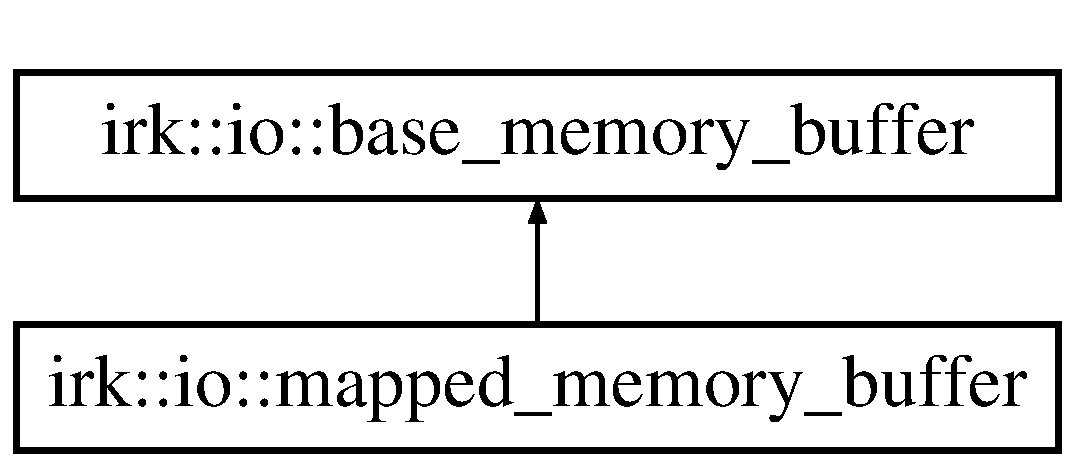
\includegraphics[height=2.000000cm]{classirk_1_1io_1_1mapped__memory__buffer}
\end{center}
\end{figure}
\subsection*{Public Types}
\begin{DoxyCompactItemize}
\item 
using \mbox{\hyperlink{classirk_1_1io_1_1mapped__memory__buffer_a8335df78a8e028b6ee8fb4011e2abfc7}{char\+\_\+type}} = char
\end{DoxyCompactItemize}
\subsection*{Public Member Functions}
\begin{DoxyCompactItemize}
\item 
\mbox{\hyperlink{classirk_1_1io_1_1mapped__memory__buffer_a4484625f0aff60adefca35d8933bc9ff}{mapped\+\_\+memory\+\_\+buffer}} (fs\+::path file)
\item 
virtual \mbox{\hyperlink{classirk_1_1io_1_1base__memory__buffer_a1b539180df4274dd4ad0402a0ac821ec}{char\+\_\+type}} $\ast$ \mbox{\hyperlink{classirk_1_1io_1_1mapped__memory__buffer_a2b731cf50320c20fb271bdd5c6f384c4}{data}} ()
\item 
virtual const \mbox{\hyperlink{classirk_1_1io_1_1base__memory__buffer_a1b539180df4274dd4ad0402a0ac821ec}{char\+\_\+type}} $\ast$ \mbox{\hyperlink{classirk_1_1io_1_1mapped__memory__buffer_ab4bbb25488358a3d527d45d16a845fb6}{data}} () const
\item 
virtual std\+::size\+\_\+t \mbox{\hyperlink{classirk_1_1io_1_1mapped__memory__buffer_ae64bb8d5018d83bd9feb605704bb0c82}{size}} () const
\end{DoxyCompactItemize}


\subsection{Member Typedef Documentation}
\mbox{\Hypertarget{classirk_1_1io_1_1mapped__memory__buffer_a8335df78a8e028b6ee8fb4011e2abfc7}\label{classirk_1_1io_1_1mapped__memory__buffer_a8335df78a8e028b6ee8fb4011e2abfc7}} 
\index{irk\+::io\+::mapped\+\_\+memory\+\_\+buffer@{irk\+::io\+::mapped\+\_\+memory\+\_\+buffer}!char\+\_\+type@{char\+\_\+type}}
\index{char\+\_\+type@{char\+\_\+type}!irk\+::io\+::mapped\+\_\+memory\+\_\+buffer@{irk\+::io\+::mapped\+\_\+memory\+\_\+buffer}}
\subsubsection{\texorpdfstring{char\+\_\+type}{char\_type}}
{\footnotesize\ttfamily using \mbox{\hyperlink{classirk_1_1io_1_1mapped__memory__buffer_a8335df78a8e028b6ee8fb4011e2abfc7}{irk\+::io\+::mapped\+\_\+memory\+\_\+buffer\+::char\+\_\+type}} =  char}



\subsection{Constructor \& Destructor Documentation}
\mbox{\Hypertarget{classirk_1_1io_1_1mapped__memory__buffer_a4484625f0aff60adefca35d8933bc9ff}\label{classirk_1_1io_1_1mapped__memory__buffer_a4484625f0aff60adefca35d8933bc9ff}} 
\index{irk\+::io\+::mapped\+\_\+memory\+\_\+buffer@{irk\+::io\+::mapped\+\_\+memory\+\_\+buffer}!mapped\+\_\+memory\+\_\+buffer@{mapped\+\_\+memory\+\_\+buffer}}
\index{mapped\+\_\+memory\+\_\+buffer@{mapped\+\_\+memory\+\_\+buffer}!irk\+::io\+::mapped\+\_\+memory\+\_\+buffer@{irk\+::io\+::mapped\+\_\+memory\+\_\+buffer}}
\subsubsection{\texorpdfstring{mapped\+\_\+memory\+\_\+buffer()}{mapped\_memory\_buffer()}}
{\footnotesize\ttfamily irk\+::io\+::mapped\+\_\+memory\+\_\+buffer\+::mapped\+\_\+memory\+\_\+buffer (\begin{DoxyParamCaption}\item[{fs\+::path}]{file }\end{DoxyParamCaption})\hspace{0.3cm}{\ttfamily [inline]}}



\subsection{Member Function Documentation}
\mbox{\Hypertarget{classirk_1_1io_1_1mapped__memory__buffer_a2b731cf50320c20fb271bdd5c6f384c4}\label{classirk_1_1io_1_1mapped__memory__buffer_a2b731cf50320c20fb271bdd5c6f384c4}} 
\index{irk\+::io\+::mapped\+\_\+memory\+\_\+buffer@{irk\+::io\+::mapped\+\_\+memory\+\_\+buffer}!data@{data}}
\index{data@{data}!irk\+::io\+::mapped\+\_\+memory\+\_\+buffer@{irk\+::io\+::mapped\+\_\+memory\+\_\+buffer}}
\subsubsection{\texorpdfstring{data()}{data()}\hspace{0.1cm}{\footnotesize\ttfamily [1/2]}}
{\footnotesize\ttfamily virtual \mbox{\hyperlink{classirk_1_1io_1_1base__memory__buffer_a1b539180df4274dd4ad0402a0ac821ec}{char\+\_\+type}}$\ast$ irk\+::io\+::mapped\+\_\+memory\+\_\+buffer\+::data (\begin{DoxyParamCaption}{ }\end{DoxyParamCaption})\hspace{0.3cm}{\ttfamily [inline]}, {\ttfamily [virtual]}}



Implements \mbox{\hyperlink{classirk_1_1io_1_1base__memory__buffer_ae8247b83aae579cbc04b5432bd4858cc}{irk\+::io\+::base\+\_\+memory\+\_\+buffer}}.

\mbox{\Hypertarget{classirk_1_1io_1_1mapped__memory__buffer_ab4bbb25488358a3d527d45d16a845fb6}\label{classirk_1_1io_1_1mapped__memory__buffer_ab4bbb25488358a3d527d45d16a845fb6}} 
\index{irk\+::io\+::mapped\+\_\+memory\+\_\+buffer@{irk\+::io\+::mapped\+\_\+memory\+\_\+buffer}!data@{data}}
\index{data@{data}!irk\+::io\+::mapped\+\_\+memory\+\_\+buffer@{irk\+::io\+::mapped\+\_\+memory\+\_\+buffer}}
\subsubsection{\texorpdfstring{data()}{data()}\hspace{0.1cm}{\footnotesize\ttfamily [2/2]}}
{\footnotesize\ttfamily virtual const \mbox{\hyperlink{classirk_1_1io_1_1base__memory__buffer_a1b539180df4274dd4ad0402a0ac821ec}{char\+\_\+type}}$\ast$ irk\+::io\+::mapped\+\_\+memory\+\_\+buffer\+::data (\begin{DoxyParamCaption}{ }\end{DoxyParamCaption}) const\hspace{0.3cm}{\ttfamily [inline]}, {\ttfamily [virtual]}}



Implements \mbox{\hyperlink{classirk_1_1io_1_1base__memory__buffer_a87bbff1a6d211e26f0c0aa924a980b9e}{irk\+::io\+::base\+\_\+memory\+\_\+buffer}}.

\mbox{\Hypertarget{classirk_1_1io_1_1mapped__memory__buffer_ae64bb8d5018d83bd9feb605704bb0c82}\label{classirk_1_1io_1_1mapped__memory__buffer_ae64bb8d5018d83bd9feb605704bb0c82}} 
\index{irk\+::io\+::mapped\+\_\+memory\+\_\+buffer@{irk\+::io\+::mapped\+\_\+memory\+\_\+buffer}!size@{size}}
\index{size@{size}!irk\+::io\+::mapped\+\_\+memory\+\_\+buffer@{irk\+::io\+::mapped\+\_\+memory\+\_\+buffer}}
\subsubsection{\texorpdfstring{size()}{size()}}
{\footnotesize\ttfamily virtual std\+::size\+\_\+t irk\+::io\+::mapped\+\_\+memory\+\_\+buffer\+::size (\begin{DoxyParamCaption}{ }\end{DoxyParamCaption}) const\hspace{0.3cm}{\ttfamily [inline]}, {\ttfamily [virtual]}}



Implements \mbox{\hyperlink{classirk_1_1io_1_1base__memory__buffer_ae634ab934981e7e4baf5e1e67ef3b006}{irk\+::io\+::base\+\_\+memory\+\_\+buffer}}.



The documentation for this class was generated from the following file\+:\begin{DoxyCompactItemize}
\item 
include/irkit/io/\mbox{\hyperlink{memorybuffer_8hpp}{memorybuffer.\+hpp}}\end{DoxyCompactItemize}

\hypertarget{classirk_1_1memory__view}{}\section{irk\+:\+:memory\+\_\+view Class Reference}
\label{classirk_1_1memory__view}\index{irk\+::memory\+\_\+view@{irk\+::memory\+\_\+view}}


A base class for all types of memory views.  




{\ttfamily \#include $<$memoryview.\+hpp$>$}

\subsection*{Classes}
\begin{DoxyCompactItemize}
\item 
struct \mbox{\hyperlink{structirk_1_1memory__view_1_1concept}{concept}}
\item 
class \mbox{\hyperlink{classirk_1_1memory__view_1_1model}{model}}
\end{DoxyCompactItemize}
\subsection*{Public Types}
\begin{DoxyCompactItemize}
\item 
using \mbox{\hyperlink{classirk_1_1memory__view_afbb67d0d922dfae3ea53d41706bd8eea}{slice\+\_\+end}} = std\+::optional$<$ std\+::ptrdiff\+\_\+t $>$
\item 
using \mbox{\hyperlink{classirk_1_1memory__view_ac0c1d9600bf81e8cb861a89ab104a43c}{slice\+\_\+type}} = std\+::pair$<$ \mbox{\hyperlink{classirk_1_1memory__view_afbb67d0d922dfae3ea53d41706bd8eea}{slice\+\_\+end}}, \mbox{\hyperlink{classirk_1_1memory__view_afbb67d0d922dfae3ea53d41706bd8eea}{slice\+\_\+end}} $>$
\item 
using \mbox{\hyperlink{classirk_1_1memory__view_a425bdc98ffa1c1c6cb018b3b4ad64317}{iterator}} = const char $\ast$
\end{DoxyCompactItemize}
\subsection*{Public Member Functions}
\begin{DoxyCompactItemize}
\item 
{\footnotesize template$<$class source\+\_\+type $>$ }\\\mbox{\hyperlink{classirk_1_1memory__view_a25918933f1b7944199c65654517d2a72}{memory\+\_\+view}} (\mbox{\hyperlink{irk-score_8cpp_a73f57f67fb1e33bdbfd80bfba2fc9ffe}{source\+\_\+type}} source)
\begin{DoxyCompactList}\small\item\em Creates a memory view. \end{DoxyCompactList}\item 
\mbox{\hyperlink{classirk_1_1memory__view_a8530b1378e96dd8f82416b56248cf9b1}{memory\+\_\+view}} ()=default
\item 
\mbox{\hyperlink{classirk_1_1memory__view_ac1160e860abc324f74e19fdb4eb7b6f1}{memory\+\_\+view}} (const \mbox{\hyperlink{classirk_1_1memory__view}{memory\+\_\+view}} \&)=default
\item 
\mbox{\hyperlink{classirk_1_1memory__view_ac057f2cd40190acb964acd24e1fdeac1}{memory\+\_\+view}} (\mbox{\hyperlink{classirk_1_1memory__view}{memory\+\_\+view}} \&\&other)=default
\item 
\mbox{\hyperlink{classirk_1_1memory__view}{memory\+\_\+view}} \& \mbox{\hyperlink{classirk_1_1memory__view_a3e72e258a7d53b02e292b3875cd5add3}{operator=}} (const \mbox{\hyperlink{classirk_1_1memory__view}{memory\+\_\+view}} \&)=default
\item 
\mbox{\hyperlink{classirk_1_1memory__view}{memory\+\_\+view}} \& \mbox{\hyperlink{classirk_1_1memory__view_ab9e565bd6ca92f5e16b5741f6ef8a708}{operator=}} (\mbox{\hyperlink{classirk_1_1memory__view}{memory\+\_\+view}} \&\&) noexcept=default
\item 
\mbox{\hyperlink{classirk_1_1memory__view_a06b0a6d7117a0edd95323c423ef5c34c}{$\sim$memory\+\_\+view}} ()=default
\item 
const char $\ast$ \mbox{\hyperlink{classirk_1_1memory__view_ab55150c13cf7e380aaaeda8d70d24bed}{data}} () const
\begin{DoxyCompactList}\small\item\em Returns a pointer to the underlying data. \end{DoxyCompactList}\item 
std\+::ptrdiff\+\_\+t \mbox{\hyperlink{classirk_1_1memory__view_af9ae4528f4f33cf24ab65115f96b7e18}{size}} () const
\begin{DoxyCompactList}\small\item\em Returns the number of characters in the memory area. \end{DoxyCompactList}\item 
const char \& \mbox{\hyperlink{classirk_1_1memory__view_a21ac618a1eaddf6665148d186f3f67a4}{operator\mbox{[}$\,$\mbox{]}}} (std\+::ptrdiff\+\_\+t n) const
\begin{DoxyCompactList}\small\item\em Returns a character at offset {\ttfamily n} in the memory. \end{DoxyCompactList}\item 
\mbox{\hyperlink{classirk_1_1memory__view}{irk\+::memory\+\_\+view}} \mbox{\hyperlink{classirk_1_1memory__view_a5edb4d5f580fdcc20f131e8980d1f7aa}{range}} (std\+::ptrdiff\+\_\+t first, std\+::ptrdiff\+\_\+t \mbox{\hyperlink{classirk_1_1memory__view_af9ae4528f4f33cf24ab65115f96b7e18}{size}}) const
\begin{DoxyCompactList}\small\item\em Returns a new memory view defined by the given range. \end{DoxyCompactList}\item 
\mbox{\hyperlink{classirk_1_1memory__view}{irk\+::memory\+\_\+view}} \mbox{\hyperlink{classirk_1_1memory__view_ae16ba32b9419a8918762132186a00463}{operator\mbox{[}$\,$\mbox{]}}} (\mbox{\hyperlink{classirk_1_1memory__view_ac0c1d9600bf81e8cb861a89ab104a43c}{slice\+\_\+type}} slice) const
\begin{DoxyCompactList}\small\item\em Returns a new memory view defined by the given slice. \end{DoxyCompactList}\item 
\mbox{\hyperlink{classirk_1_1memory__view}{irk\+::memory\+\_\+view}} \mbox{\hyperlink{classirk_1_1memory__view_a3512cd124a9e37db75e295e1ff9fcf96}{operator()}} (std\+::ptrdiff\+\_\+t lo, std\+::ptrdiff\+\_\+t hi) const
\begin{DoxyCompactList}\small\item\em Returns a new memory view defined by a half-\/open range \mbox{[}lo, hi). \end{DoxyCompactList}\item 
\mbox{\hyperlink{classirk_1_1memory__view}{irk\+::memory\+\_\+view}} \mbox{\hyperlink{classirk_1_1memory__view_a08de0b791c9f50ad1b646e85fb67e734}{operator()}} (std\+::ptrdiff\+\_\+t cut) const
\begin{DoxyCompactList}\small\item\em Returns a new memory view defined by the given cut. \end{DoxyCompactList}\item 
{\footnotesize template$<$class T , class Cast\+Fn  = reinterpret\+\_\+cast\+\_\+fn$<$\+T$>$$>$ }\\T \mbox{\hyperlink{classirk_1_1memory__view_ae9d042dabe259ef35ac2fec319c40b57}{as}} (Cast\+Fn cast\+\_\+fn=\mbox{\hyperlink{structirk_1_1reinterpret__cast__fn}{reinterpret\+\_\+cast\+\_\+fn}}$<$ T $>$\{\}) const
\item 
\mbox{\hyperlink{classirk_1_1memory__view_a425bdc98ffa1c1c6cb018b3b4ad64317}{iterator}} \mbox{\hyperlink{classirk_1_1memory__view_a41d2227984ac0284ec52588a57bd297c}{begin}} () const
\item 
\mbox{\hyperlink{classirk_1_1memory__view_a425bdc98ffa1c1c6cb018b3b4ad64317}{iterator}} \mbox{\hyperlink{classirk_1_1memory__view_a393e04a837ff706e408fbea11219d7ed}{end}} () const
\item 
auto \mbox{\hyperlink{classirk_1_1memory__view_a4e324d9edda27a3125d2ab364d1e5552}{stream}} () const
\end{DoxyCompactItemize}


\subsection{Detailed Description}
A base class for all types of memory views. 

A memory view is an abstraction for accessing any memory area, be it in main memory, or on disk, or via a memory mapped file. The constructor accepts different types of memory sources that implement memory access details. These types are hidden with type erasure\+: only the constructor is a template, and {\ttfamily \mbox{\hyperlink{classirk_1_1memory__view}{memory\+\_\+view}}} type can be used polymorphically. 

\subsection{Member Typedef Documentation}
\mbox{\Hypertarget{classirk_1_1memory__view_a425bdc98ffa1c1c6cb018b3b4ad64317}\label{classirk_1_1memory__view_a425bdc98ffa1c1c6cb018b3b4ad64317}} 
\index{irk\+::memory\+\_\+view@{irk\+::memory\+\_\+view}!iterator@{iterator}}
\index{iterator@{iterator}!irk\+::memory\+\_\+view@{irk\+::memory\+\_\+view}}
\subsubsection{\texorpdfstring{iterator}{iterator}}
{\footnotesize\ttfamily using \mbox{\hyperlink{classirk_1_1memory__view_a425bdc98ffa1c1c6cb018b3b4ad64317}{irk\+::memory\+\_\+view\+::iterator}} =  const char$\ast$}

\mbox{\Hypertarget{classirk_1_1memory__view_afbb67d0d922dfae3ea53d41706bd8eea}\label{classirk_1_1memory__view_afbb67d0d922dfae3ea53d41706bd8eea}} 
\index{irk\+::memory\+\_\+view@{irk\+::memory\+\_\+view}!slice\+\_\+end@{slice\+\_\+end}}
\index{slice\+\_\+end@{slice\+\_\+end}!irk\+::memory\+\_\+view@{irk\+::memory\+\_\+view}}
\subsubsection{\texorpdfstring{slice\+\_\+end}{slice\_end}}
{\footnotesize\ttfamily using \mbox{\hyperlink{classirk_1_1memory__view_afbb67d0d922dfae3ea53d41706bd8eea}{irk\+::memory\+\_\+view\+::slice\+\_\+end}} =  std\+::optional$<$std\+::ptrdiff\+\_\+t$>$}

\mbox{\Hypertarget{classirk_1_1memory__view_ac0c1d9600bf81e8cb861a89ab104a43c}\label{classirk_1_1memory__view_ac0c1d9600bf81e8cb861a89ab104a43c}} 
\index{irk\+::memory\+\_\+view@{irk\+::memory\+\_\+view}!slice\+\_\+type@{slice\+\_\+type}}
\index{slice\+\_\+type@{slice\+\_\+type}!irk\+::memory\+\_\+view@{irk\+::memory\+\_\+view}}
\subsubsection{\texorpdfstring{slice\+\_\+type}{slice\_type}}
{\footnotesize\ttfamily using \mbox{\hyperlink{classirk_1_1memory__view_ac0c1d9600bf81e8cb861a89ab104a43c}{irk\+::memory\+\_\+view\+::slice\+\_\+type}} =  std\+::pair$<$\mbox{\hyperlink{classirk_1_1memory__view_afbb67d0d922dfae3ea53d41706bd8eea}{slice\+\_\+end}}, \mbox{\hyperlink{classirk_1_1memory__view_afbb67d0d922dfae3ea53d41706bd8eea}{slice\+\_\+end}}$>$}



\subsection{Constructor \& Destructor Documentation}
\mbox{\Hypertarget{classirk_1_1memory__view_a25918933f1b7944199c65654517d2a72}\label{classirk_1_1memory__view_a25918933f1b7944199c65654517d2a72}} 
\index{irk\+::memory\+\_\+view@{irk\+::memory\+\_\+view}!memory\+\_\+view@{memory\+\_\+view}}
\index{memory\+\_\+view@{memory\+\_\+view}!irk\+::memory\+\_\+view@{irk\+::memory\+\_\+view}}
\subsubsection{\texorpdfstring{memory\+\_\+view()}{memory\_view()}\hspace{0.1cm}{\footnotesize\ttfamily [1/4]}}
{\footnotesize\ttfamily template$<$class source\+\_\+type $>$ \\
irk\+::memory\+\_\+view\+::memory\+\_\+view (\begin{DoxyParamCaption}\item[{\mbox{\hyperlink{irk-score_8cpp_a73f57f67fb1e33bdbfd80bfba2fc9ffe}{source\+\_\+type}}}]{source }\end{DoxyParamCaption})\hspace{0.3cm}{\ttfamily [inline]}, {\ttfamily [explicit]}}



Creates a memory view. 


\begin{DoxyTemplParams}{Template Parameters}
{\em source\+\_\+type} & a memory source type \\
\hline
\end{DoxyTemplParams}

\begin{DoxyParams}{Parameters}
{\em source} & a copy of this will be created on heap to support polymorphic usage with value semantic. \\
\hline
\end{DoxyParams}
\mbox{\Hypertarget{classirk_1_1memory__view_a8530b1378e96dd8f82416b56248cf9b1}\label{classirk_1_1memory__view_a8530b1378e96dd8f82416b56248cf9b1}} 
\index{irk\+::memory\+\_\+view@{irk\+::memory\+\_\+view}!memory\+\_\+view@{memory\+\_\+view}}
\index{memory\+\_\+view@{memory\+\_\+view}!irk\+::memory\+\_\+view@{irk\+::memory\+\_\+view}}
\subsubsection{\texorpdfstring{memory\+\_\+view()}{memory\_view()}\hspace{0.1cm}{\footnotesize\ttfamily [2/4]}}
{\footnotesize\ttfamily irk\+::memory\+\_\+view\+::memory\+\_\+view (\begin{DoxyParamCaption}{ }\end{DoxyParamCaption})\hspace{0.3cm}{\ttfamily [default]}}

\mbox{\Hypertarget{classirk_1_1memory__view_ac1160e860abc324f74e19fdb4eb7b6f1}\label{classirk_1_1memory__view_ac1160e860abc324f74e19fdb4eb7b6f1}} 
\index{irk\+::memory\+\_\+view@{irk\+::memory\+\_\+view}!memory\+\_\+view@{memory\+\_\+view}}
\index{memory\+\_\+view@{memory\+\_\+view}!irk\+::memory\+\_\+view@{irk\+::memory\+\_\+view}}
\subsubsection{\texorpdfstring{memory\+\_\+view()}{memory\_view()}\hspace{0.1cm}{\footnotesize\ttfamily [3/4]}}
{\footnotesize\ttfamily irk\+::memory\+\_\+view\+::memory\+\_\+view (\begin{DoxyParamCaption}\item[{const \mbox{\hyperlink{classirk_1_1memory__view}{memory\+\_\+view}} \&}]{ }\end{DoxyParamCaption})\hspace{0.3cm}{\ttfamily [default]}}

\mbox{\Hypertarget{classirk_1_1memory__view_ac057f2cd40190acb964acd24e1fdeac1}\label{classirk_1_1memory__view_ac057f2cd40190acb964acd24e1fdeac1}} 
\index{irk\+::memory\+\_\+view@{irk\+::memory\+\_\+view}!memory\+\_\+view@{memory\+\_\+view}}
\index{memory\+\_\+view@{memory\+\_\+view}!irk\+::memory\+\_\+view@{irk\+::memory\+\_\+view}}
\subsubsection{\texorpdfstring{memory\+\_\+view()}{memory\_view()}\hspace{0.1cm}{\footnotesize\ttfamily [4/4]}}
{\footnotesize\ttfamily irk\+::memory\+\_\+view\+::memory\+\_\+view (\begin{DoxyParamCaption}\item[{\mbox{\hyperlink{classirk_1_1memory__view}{memory\+\_\+view}} \&\&}]{other }\end{DoxyParamCaption})\hspace{0.3cm}{\ttfamily [default]}}

\mbox{\Hypertarget{classirk_1_1memory__view_a06b0a6d7117a0edd95323c423ef5c34c}\label{classirk_1_1memory__view_a06b0a6d7117a0edd95323c423ef5c34c}} 
\index{irk\+::memory\+\_\+view@{irk\+::memory\+\_\+view}!````~memory\+\_\+view@{$\sim$memory\+\_\+view}}
\index{````~memory\+\_\+view@{$\sim$memory\+\_\+view}!irk\+::memory\+\_\+view@{irk\+::memory\+\_\+view}}
\subsubsection{\texorpdfstring{$\sim$memory\+\_\+view()}{~memory\_view()}}
{\footnotesize\ttfamily irk\+::memory\+\_\+view\+::$\sim$memory\+\_\+view (\begin{DoxyParamCaption}{ }\end{DoxyParamCaption})\hspace{0.3cm}{\ttfamily [default]}}



\subsection{Member Function Documentation}
\mbox{\Hypertarget{classirk_1_1memory__view_ae9d042dabe259ef35ac2fec319c40b57}\label{classirk_1_1memory__view_ae9d042dabe259ef35ac2fec319c40b57}} 
\index{irk\+::memory\+\_\+view@{irk\+::memory\+\_\+view}!as@{as}}
\index{as@{as}!irk\+::memory\+\_\+view@{irk\+::memory\+\_\+view}}
\subsubsection{\texorpdfstring{as()}{as()}}
{\footnotesize\ttfamily template$<$class T , class Cast\+Fn  = reinterpret\+\_\+cast\+\_\+fn$<$\+T$>$$>$ \\
T irk\+::memory\+\_\+view\+::as (\begin{DoxyParamCaption}\item[{Cast\+Fn}]{cast\+\_\+fn = {\ttfamily \mbox{\hyperlink{structirk_1_1reinterpret__cast__fn}{reinterpret\+\_\+cast\+\_\+fn}}$<$T$>$\{\}} }\end{DoxyParamCaption}) const\hspace{0.3cm}{\ttfamily [inline]}}

\mbox{\Hypertarget{classirk_1_1memory__view_a41d2227984ac0284ec52588a57bd297c}\label{classirk_1_1memory__view_a41d2227984ac0284ec52588a57bd297c}} 
\index{irk\+::memory\+\_\+view@{irk\+::memory\+\_\+view}!begin@{begin}}
\index{begin@{begin}!irk\+::memory\+\_\+view@{irk\+::memory\+\_\+view}}
\subsubsection{\texorpdfstring{begin()}{begin()}}
{\footnotesize\ttfamily \mbox{\hyperlink{classirk_1_1memory__view_a425bdc98ffa1c1c6cb018b3b4ad64317}{iterator}} irk\+::memory\+\_\+view\+::begin (\begin{DoxyParamCaption}{ }\end{DoxyParamCaption}) const\hspace{0.3cm}{\ttfamily [inline]}}

\mbox{\Hypertarget{classirk_1_1memory__view_ab55150c13cf7e380aaaeda8d70d24bed}\label{classirk_1_1memory__view_ab55150c13cf7e380aaaeda8d70d24bed}} 
\index{irk\+::memory\+\_\+view@{irk\+::memory\+\_\+view}!data@{data}}
\index{data@{data}!irk\+::memory\+\_\+view@{irk\+::memory\+\_\+view}}
\subsubsection{\texorpdfstring{data()}{data()}}
{\footnotesize\ttfamily const char$\ast$ irk\+::memory\+\_\+view\+::data (\begin{DoxyParamCaption}{ }\end{DoxyParamCaption}) const\hspace{0.3cm}{\ttfamily [inline]}}



Returns a pointer to the underlying data. 

The source is expected to return a pointer of contiguous data in memory (or memory mapped file). Thus, if a source loads data lazily, it must first load the entire data and return its pointer. To avoid such inefficiency, e.\+g., if data is meant to be accessed sequentially, use \mbox{\hyperlink{classirk_1_1memory__view_a41d2227984ac0284ec52588a57bd297c}{begin()}} and \mbox{\hyperlink{classirk_1_1memory__view_a393e04a837ff706e408fbea11219d7ed}{end()}}, or \mbox{\hyperlink{classirk_1_1memory__view_a21ac618a1eaddf6665148d186f3f67a4}{operator\mbox{[}\mbox{]}}} instead. \mbox{\Hypertarget{classirk_1_1memory__view_a393e04a837ff706e408fbea11219d7ed}\label{classirk_1_1memory__view_a393e04a837ff706e408fbea11219d7ed}} 
\index{irk\+::memory\+\_\+view@{irk\+::memory\+\_\+view}!end@{end}}
\index{end@{end}!irk\+::memory\+\_\+view@{irk\+::memory\+\_\+view}}
\subsubsection{\texorpdfstring{end()}{end()}}
{\footnotesize\ttfamily \mbox{\hyperlink{classirk_1_1memory__view_a425bdc98ffa1c1c6cb018b3b4ad64317}{iterator}} irk\+::memory\+\_\+view\+::end (\begin{DoxyParamCaption}{ }\end{DoxyParamCaption}) const\hspace{0.3cm}{\ttfamily [inline]}}

\mbox{\Hypertarget{classirk_1_1memory__view_a3512cd124a9e37db75e295e1ff9fcf96}\label{classirk_1_1memory__view_a3512cd124a9e37db75e295e1ff9fcf96}} 
\index{irk\+::memory\+\_\+view@{irk\+::memory\+\_\+view}!operator()@{operator()}}
\index{operator()@{operator()}!irk\+::memory\+\_\+view@{irk\+::memory\+\_\+view}}
\subsubsection{\texorpdfstring{operator()()}{operator()()}\hspace{0.1cm}{\footnotesize\ttfamily [1/2]}}
{\footnotesize\ttfamily \mbox{\hyperlink{classirk_1_1memory__view}{irk\+::memory\+\_\+view}} irk\+::memory\+\_\+view\+::operator() (\begin{DoxyParamCaption}\item[{std\+::ptrdiff\+\_\+t}]{lo,  }\item[{std\+::ptrdiff\+\_\+t}]{hi }\end{DoxyParamCaption}) const\hspace{0.3cm}{\ttfamily [inline]}}



Returns a new memory view defined by a half-\/open range \mbox{[}lo, hi). 

\mbox{\Hypertarget{classirk_1_1memory__view_a08de0b791c9f50ad1b646e85fb67e734}\label{classirk_1_1memory__view_a08de0b791c9f50ad1b646e85fb67e734}} 
\index{irk\+::memory\+\_\+view@{irk\+::memory\+\_\+view}!operator()@{operator()}}
\index{operator()@{operator()}!irk\+::memory\+\_\+view@{irk\+::memory\+\_\+view}}
\subsubsection{\texorpdfstring{operator()()}{operator()()}\hspace{0.1cm}{\footnotesize\ttfamily [2/2]}}
{\footnotesize\ttfamily \mbox{\hyperlink{classirk_1_1memory__view}{irk\+::memory\+\_\+view}} irk\+::memory\+\_\+view\+::operator() (\begin{DoxyParamCaption}\item[{std\+::ptrdiff\+\_\+t}]{cut }\end{DoxyParamCaption}) const\hspace{0.3cm}{\ttfamily [inline]}}



Returns a new memory view defined by the given cut. 

\mbox{\Hypertarget{classirk_1_1memory__view_a3e72e258a7d53b02e292b3875cd5add3}\label{classirk_1_1memory__view_a3e72e258a7d53b02e292b3875cd5add3}} 
\index{irk\+::memory\+\_\+view@{irk\+::memory\+\_\+view}!operator=@{operator=}}
\index{operator=@{operator=}!irk\+::memory\+\_\+view@{irk\+::memory\+\_\+view}}
\subsubsection{\texorpdfstring{operator=()}{operator=()}\hspace{0.1cm}{\footnotesize\ttfamily [1/2]}}
{\footnotesize\ttfamily \mbox{\hyperlink{classirk_1_1memory__view}{memory\+\_\+view}}\& irk\+::memory\+\_\+view\+::operator= (\begin{DoxyParamCaption}\item[{const \mbox{\hyperlink{classirk_1_1memory__view}{memory\+\_\+view}} \&}]{ }\end{DoxyParamCaption})\hspace{0.3cm}{\ttfamily [default]}}

\mbox{\Hypertarget{classirk_1_1memory__view_ab9e565bd6ca92f5e16b5741f6ef8a708}\label{classirk_1_1memory__view_ab9e565bd6ca92f5e16b5741f6ef8a708}} 
\index{irk\+::memory\+\_\+view@{irk\+::memory\+\_\+view}!operator=@{operator=}}
\index{operator=@{operator=}!irk\+::memory\+\_\+view@{irk\+::memory\+\_\+view}}
\subsubsection{\texorpdfstring{operator=()}{operator=()}\hspace{0.1cm}{\footnotesize\ttfamily [2/2]}}
{\footnotesize\ttfamily \mbox{\hyperlink{classirk_1_1memory__view}{memory\+\_\+view}}\& irk\+::memory\+\_\+view\+::operator= (\begin{DoxyParamCaption}\item[{\mbox{\hyperlink{classirk_1_1memory__view}{memory\+\_\+view}} \&\&}]{ }\end{DoxyParamCaption})\hspace{0.3cm}{\ttfamily [default]}, {\ttfamily [noexcept]}}

\mbox{\Hypertarget{classirk_1_1memory__view_a21ac618a1eaddf6665148d186f3f67a4}\label{classirk_1_1memory__view_a21ac618a1eaddf6665148d186f3f67a4}} 
\index{irk\+::memory\+\_\+view@{irk\+::memory\+\_\+view}!operator\mbox{[}\mbox{]}@{operator[]}}
\index{operator\mbox{[}\mbox{]}@{operator[]}!irk\+::memory\+\_\+view@{irk\+::memory\+\_\+view}}
\subsubsection{\texorpdfstring{operator[]()}{operator[]()}\hspace{0.1cm}{\footnotesize\ttfamily [1/2]}}
{\footnotesize\ttfamily const char\& irk\+::memory\+\_\+view\+::operator\mbox{[}$\,$\mbox{]} (\begin{DoxyParamCaption}\item[{std\+::ptrdiff\+\_\+t}]{n }\end{DoxyParamCaption}) const\hspace{0.3cm}{\ttfamily [inline]}}



Returns a character at offset {\ttfamily n} in the memory. 

\mbox{\Hypertarget{classirk_1_1memory__view_ae16ba32b9419a8918762132186a00463}\label{classirk_1_1memory__view_ae16ba32b9419a8918762132186a00463}} 
\index{irk\+::memory\+\_\+view@{irk\+::memory\+\_\+view}!operator\mbox{[}\mbox{]}@{operator[]}}
\index{operator\mbox{[}\mbox{]}@{operator[]}!irk\+::memory\+\_\+view@{irk\+::memory\+\_\+view}}
\subsubsection{\texorpdfstring{operator[]()}{operator[]()}\hspace{0.1cm}{\footnotesize\ttfamily [2/2]}}
{\footnotesize\ttfamily \mbox{\hyperlink{classirk_1_1memory__view}{irk\+::memory\+\_\+view}} irk\+::memory\+\_\+view\+::operator\mbox{[}$\,$\mbox{]} (\begin{DoxyParamCaption}\item[{\mbox{\hyperlink{classirk_1_1memory__view_ac0c1d9600bf81e8cb861a89ab104a43c}{slice\+\_\+type}}}]{slice }\end{DoxyParamCaption}) const\hspace{0.3cm}{\ttfamily [inline]}}



Returns a new memory view defined by the given slice. 

\mbox{\Hypertarget{classirk_1_1memory__view_a5edb4d5f580fdcc20f131e8980d1f7aa}\label{classirk_1_1memory__view_a5edb4d5f580fdcc20f131e8980d1f7aa}} 
\index{irk\+::memory\+\_\+view@{irk\+::memory\+\_\+view}!range@{range}}
\index{range@{range}!irk\+::memory\+\_\+view@{irk\+::memory\+\_\+view}}
\subsubsection{\texorpdfstring{range()}{range()}}
{\footnotesize\ttfamily \mbox{\hyperlink{classirk_1_1memory__view}{irk\+::memory\+\_\+view}} irk\+::memory\+\_\+view\+::range (\begin{DoxyParamCaption}\item[{std\+::ptrdiff\+\_\+t}]{first,  }\item[{std\+::ptrdiff\+\_\+t}]{size }\end{DoxyParamCaption}) const\hspace{0.3cm}{\ttfamily [inline]}}



Returns a new memory view defined by the given range. 

\mbox{\Hypertarget{classirk_1_1memory__view_af9ae4528f4f33cf24ab65115f96b7e18}\label{classirk_1_1memory__view_af9ae4528f4f33cf24ab65115f96b7e18}} 
\index{irk\+::memory\+\_\+view@{irk\+::memory\+\_\+view}!size@{size}}
\index{size@{size}!irk\+::memory\+\_\+view@{irk\+::memory\+\_\+view}}
\subsubsection{\texorpdfstring{size()}{size()}}
{\footnotesize\ttfamily std\+::ptrdiff\+\_\+t irk\+::memory\+\_\+view\+::size (\begin{DoxyParamCaption}{ }\end{DoxyParamCaption}) const\hspace{0.3cm}{\ttfamily [inline]}}



Returns the number of characters in the memory area. 

\mbox{\Hypertarget{classirk_1_1memory__view_a4e324d9edda27a3125d2ab364d1e5552}\label{classirk_1_1memory__view_a4e324d9edda27a3125d2ab364d1e5552}} 
\index{irk\+::memory\+\_\+view@{irk\+::memory\+\_\+view}!stream@{stream}}
\index{stream@{stream}!irk\+::memory\+\_\+view@{irk\+::memory\+\_\+view}}
\subsubsection{\texorpdfstring{stream()}{stream()}}
{\footnotesize\ttfamily auto irk\+::memory\+\_\+view\+::stream (\begin{DoxyParamCaption}{ }\end{DoxyParamCaption}) const\hspace{0.3cm}{\ttfamily [inline]}}



The documentation for this class was generated from the following file\+:\begin{DoxyCompactItemize}
\item 
include/irkit/\mbox{\hyperlink{memoryview_8hpp}{memoryview.\+hpp}}\end{DoxyCompactItemize}

\hypertarget{structirk_1_1index_1_1metadata}{}\section{irk\+:\+:index\+:\+:metadata Struct Reference}
\label{structirk_1_1index_1_1metadata}\index{irk\+::index\+::metadata@{irk\+::index\+::metadata}}


Container for index-\/related metadata.  




{\ttfamily \#include $<$metadata.\+hpp$>$}

\subsection*{Public Member Functions}
\begin{DoxyCompactItemize}
\item 
\mbox{\hyperlink{structirk_1_1index_1_1metadata_a9d0e997a5145a95328519290af96326c}{metadata}} (fs\+::path \mbox{\hyperlink{structirk_1_1index_1_1metadata_a355b4325c022cd152e68fc18b1775fc6}{dir}})
\end{DoxyCompactItemize}
\subsection*{Public Attributes}
\begin{DoxyCompactItemize}
\item 
fs\+::path \mbox{\hyperlink{structirk_1_1index_1_1metadata_a355b4325c022cd152e68fc18b1775fc6}{dir}}
\item 
fs\+::path \mbox{\hyperlink{structirk_1_1index_1_1metadata_a20168da918488d66694b1da2f0542b83}{doc\+\_\+ids}} = \mbox{\hyperlink{namespaceirk_1_1index_a1680416c227181a5ab2f0b0169adb11e}{irk\+::index\+::doc\+\_\+ids\+\_\+path}}(\mbox{\hyperlink{structirk_1_1index_1_1metadata_a355b4325c022cd152e68fc18b1775fc6}{dir}})
\item 
fs\+::path \mbox{\hyperlink{structirk_1_1index_1_1metadata_a249ece1de7a87e894345d7c987609e8e}{doc\+\_\+ids\+\_\+off}} = \mbox{\hyperlink{namespaceirk_1_1index_aae22e4280b8fc44a46c81159429bf889}{irk\+::index\+::doc\+\_\+ids\+\_\+off\+\_\+path}}(\mbox{\hyperlink{structirk_1_1index_1_1metadata_a355b4325c022cd152e68fc18b1775fc6}{dir}})
\item 
fs\+::path \mbox{\hyperlink{structirk_1_1index_1_1metadata_a1c98d482a721d75186ef3695d22263ea}{doc\+\_\+counts}} = \mbox{\hyperlink{namespaceirk_1_1index_aee9cb8e5de7bc61fdc17458d5b597e04}{irk\+::index\+::doc\+\_\+counts\+\_\+path}}(\mbox{\hyperlink{structirk_1_1index_1_1metadata_a355b4325c022cd152e68fc18b1775fc6}{dir}})
\item 
fs\+::path \mbox{\hyperlink{structirk_1_1index_1_1metadata_a40270e89d8b3b63d01a2c7da3a3e3748}{doc\+\_\+counts\+\_\+off}} = \mbox{\hyperlink{namespaceirk_1_1index_a5f8f21506f18df93a60b7ff061a800df}{irk\+::index\+::doc\+\_\+counts\+\_\+off\+\_\+path}}(\mbox{\hyperlink{structirk_1_1index_1_1metadata_a355b4325c022cd152e68fc18b1775fc6}{dir}})
\item 
fs\+::path \mbox{\hyperlink{structirk_1_1index_1_1metadata_ac3c1d47e784d486a72d249cc5b7675d2}{terms}} = \mbox{\hyperlink{namespaceirk_1_1index_a003bce4c8d885ec3e8ffffd7dc53222f}{irk\+::index\+::terms\+\_\+path}}(\mbox{\hyperlink{structirk_1_1index_1_1metadata_a355b4325c022cd152e68fc18b1775fc6}{dir}})
\item 
fs\+::path \mbox{\hyperlink{structirk_1_1index_1_1metadata_a620a29ca94ec440938aa5468c96a68fa}{term\+\_\+doc\+\_\+freq}} = \mbox{\hyperlink{namespaceirk_1_1index_a616162aee34d0fe0460174bab4e8e518}{irk\+::index\+::term\+\_\+doc\+\_\+freq\+\_\+path}}(\mbox{\hyperlink{structirk_1_1index_1_1metadata_a355b4325c022cd152e68fc18b1775fc6}{dir}})
\item 
fs\+::path \mbox{\hyperlink{structirk_1_1index_1_1metadata_aae05b9d0a33fd6c90f7f9be0a359ca77}{doc\+\_\+titles}} = \mbox{\hyperlink{namespaceirk_1_1index_a2c4aa814da3f9412179fe44a70fdbe94}{irk\+::index\+::titles\+\_\+path}}(\mbox{\hyperlink{structirk_1_1index_1_1metadata_a355b4325c022cd152e68fc18b1775fc6}{dir}})
\item 
fs\+::path \mbox{\hyperlink{structirk_1_1index_1_1metadata_a7aa4d97e4e11c582380ad03e18eb62bb}{doc\+\_\+sizes}} = \mbox{\hyperlink{structirk_1_1index_1_1metadata_a355b4325c022cd152e68fc18b1775fc6}{dir}} / \char`\"{}doc.\+sizes\char`\"{}
\item 
fs\+::path \mbox{\hyperlink{structirk_1_1index_1_1metadata_a9abaf09f8e29f9be71171242db8839ec}{term\+\_\+occurrences}} = \mbox{\hyperlink{namespaceirk_1_1index_a1cd8d96d17fa744fdcc7cb3321b4dd25}{irk\+::index\+::term\+\_\+occurrences\+\_\+path}}(\mbox{\hyperlink{structirk_1_1index_1_1metadata_a355b4325c022cd152e68fc18b1775fc6}{dir}})
\item 
fs\+::path \mbox{\hyperlink{structirk_1_1index_1_1metadata_a1501ec5d527da04b74af747230504ee0}{properties}} = \mbox{\hyperlink{namespaceirk_1_1index_a5880f03dd72d6ebbae004d2ab83c219e}{irk\+::index\+::properties\+\_\+path}}(\mbox{\hyperlink{structirk_1_1index_1_1metadata_a355b4325c022cd152e68fc18b1775fc6}{dir}})
\end{DoxyCompactItemize}


\subsection{Detailed Description}
Container for index-\/related metadata. 

\subsection{Constructor \& Destructor Documentation}
\mbox{\Hypertarget{structirk_1_1index_1_1metadata_a9d0e997a5145a95328519290af96326c}\label{structirk_1_1index_1_1metadata_a9d0e997a5145a95328519290af96326c}} 
\index{irk\+::index\+::metadata@{irk\+::index\+::metadata}!metadata@{metadata}}
\index{metadata@{metadata}!irk\+::index\+::metadata@{irk\+::index\+::metadata}}
\subsubsection{\texorpdfstring{metadata()}{metadata()}}
{\footnotesize\ttfamily irk\+::index\+::metadata\+::metadata (\begin{DoxyParamCaption}\item[{fs\+::path}]{dir }\end{DoxyParamCaption})\hspace{0.3cm}{\ttfamily [inline]}}



\subsection{Member Data Documentation}
\mbox{\Hypertarget{structirk_1_1index_1_1metadata_a355b4325c022cd152e68fc18b1775fc6}\label{structirk_1_1index_1_1metadata_a355b4325c022cd152e68fc18b1775fc6}} 
\index{irk\+::index\+::metadata@{irk\+::index\+::metadata}!dir@{dir}}
\index{dir@{dir}!irk\+::index\+::metadata@{irk\+::index\+::metadata}}
\subsubsection{\texorpdfstring{dir}{dir}}
{\footnotesize\ttfamily fs\+::path irk\+::index\+::metadata\+::dir}

\mbox{\Hypertarget{structirk_1_1index_1_1metadata_a1c98d482a721d75186ef3695d22263ea}\label{structirk_1_1index_1_1metadata_a1c98d482a721d75186ef3695d22263ea}} 
\index{irk\+::index\+::metadata@{irk\+::index\+::metadata}!doc\+\_\+counts@{doc\+\_\+counts}}
\index{doc\+\_\+counts@{doc\+\_\+counts}!irk\+::index\+::metadata@{irk\+::index\+::metadata}}
\subsubsection{\texorpdfstring{doc\+\_\+counts}{doc\_counts}}
{\footnotesize\ttfamily fs\+::path irk\+::index\+::metadata\+::doc\+\_\+counts = \mbox{\hyperlink{namespaceirk_1_1index_aee9cb8e5de7bc61fdc17458d5b597e04}{irk\+::index\+::doc\+\_\+counts\+\_\+path}}(\mbox{\hyperlink{structirk_1_1index_1_1metadata_a355b4325c022cd152e68fc18b1775fc6}{dir}})}

\mbox{\Hypertarget{structirk_1_1index_1_1metadata_a40270e89d8b3b63d01a2c7da3a3e3748}\label{structirk_1_1index_1_1metadata_a40270e89d8b3b63d01a2c7da3a3e3748}} 
\index{irk\+::index\+::metadata@{irk\+::index\+::metadata}!doc\+\_\+counts\+\_\+off@{doc\+\_\+counts\+\_\+off}}
\index{doc\+\_\+counts\+\_\+off@{doc\+\_\+counts\+\_\+off}!irk\+::index\+::metadata@{irk\+::index\+::metadata}}
\subsubsection{\texorpdfstring{doc\+\_\+counts\+\_\+off}{doc\_counts\_off}}
{\footnotesize\ttfamily fs\+::path irk\+::index\+::metadata\+::doc\+\_\+counts\+\_\+off = \mbox{\hyperlink{namespaceirk_1_1index_a5f8f21506f18df93a60b7ff061a800df}{irk\+::index\+::doc\+\_\+counts\+\_\+off\+\_\+path}}(\mbox{\hyperlink{structirk_1_1index_1_1metadata_a355b4325c022cd152e68fc18b1775fc6}{dir}})}

\mbox{\Hypertarget{structirk_1_1index_1_1metadata_a20168da918488d66694b1da2f0542b83}\label{structirk_1_1index_1_1metadata_a20168da918488d66694b1da2f0542b83}} 
\index{irk\+::index\+::metadata@{irk\+::index\+::metadata}!doc\+\_\+ids@{doc\+\_\+ids}}
\index{doc\+\_\+ids@{doc\+\_\+ids}!irk\+::index\+::metadata@{irk\+::index\+::metadata}}
\subsubsection{\texorpdfstring{doc\+\_\+ids}{doc\_ids}}
{\footnotesize\ttfamily fs\+::path irk\+::index\+::metadata\+::doc\+\_\+ids = \mbox{\hyperlink{namespaceirk_1_1index_a1680416c227181a5ab2f0b0169adb11e}{irk\+::index\+::doc\+\_\+ids\+\_\+path}}(\mbox{\hyperlink{structirk_1_1index_1_1metadata_a355b4325c022cd152e68fc18b1775fc6}{dir}})}

\mbox{\Hypertarget{structirk_1_1index_1_1metadata_a249ece1de7a87e894345d7c987609e8e}\label{structirk_1_1index_1_1metadata_a249ece1de7a87e894345d7c987609e8e}} 
\index{irk\+::index\+::metadata@{irk\+::index\+::metadata}!doc\+\_\+ids\+\_\+off@{doc\+\_\+ids\+\_\+off}}
\index{doc\+\_\+ids\+\_\+off@{doc\+\_\+ids\+\_\+off}!irk\+::index\+::metadata@{irk\+::index\+::metadata}}
\subsubsection{\texorpdfstring{doc\+\_\+ids\+\_\+off}{doc\_ids\_off}}
{\footnotesize\ttfamily fs\+::path irk\+::index\+::metadata\+::doc\+\_\+ids\+\_\+off = \mbox{\hyperlink{namespaceirk_1_1index_aae22e4280b8fc44a46c81159429bf889}{irk\+::index\+::doc\+\_\+ids\+\_\+off\+\_\+path}}(\mbox{\hyperlink{structirk_1_1index_1_1metadata_a355b4325c022cd152e68fc18b1775fc6}{dir}})}

\mbox{\Hypertarget{structirk_1_1index_1_1metadata_a7aa4d97e4e11c582380ad03e18eb62bb}\label{structirk_1_1index_1_1metadata_a7aa4d97e4e11c582380ad03e18eb62bb}} 
\index{irk\+::index\+::metadata@{irk\+::index\+::metadata}!doc\+\_\+sizes@{doc\+\_\+sizes}}
\index{doc\+\_\+sizes@{doc\+\_\+sizes}!irk\+::index\+::metadata@{irk\+::index\+::metadata}}
\subsubsection{\texorpdfstring{doc\+\_\+sizes}{doc\_sizes}}
{\footnotesize\ttfamily fs\+::path irk\+::index\+::metadata\+::doc\+\_\+sizes = \mbox{\hyperlink{structirk_1_1index_1_1metadata_a355b4325c022cd152e68fc18b1775fc6}{dir}} / \char`\"{}doc.\+sizes\char`\"{}}

\mbox{\Hypertarget{structirk_1_1index_1_1metadata_aae05b9d0a33fd6c90f7f9be0a359ca77}\label{structirk_1_1index_1_1metadata_aae05b9d0a33fd6c90f7f9be0a359ca77}} 
\index{irk\+::index\+::metadata@{irk\+::index\+::metadata}!doc\+\_\+titles@{doc\+\_\+titles}}
\index{doc\+\_\+titles@{doc\+\_\+titles}!irk\+::index\+::metadata@{irk\+::index\+::metadata}}
\subsubsection{\texorpdfstring{doc\+\_\+titles}{doc\_titles}}
{\footnotesize\ttfamily fs\+::path irk\+::index\+::metadata\+::doc\+\_\+titles = \mbox{\hyperlink{namespaceirk_1_1index_a2c4aa814da3f9412179fe44a70fdbe94}{irk\+::index\+::titles\+\_\+path}}(\mbox{\hyperlink{structirk_1_1index_1_1metadata_a355b4325c022cd152e68fc18b1775fc6}{dir}})}

\mbox{\Hypertarget{structirk_1_1index_1_1metadata_a1501ec5d527da04b74af747230504ee0}\label{structirk_1_1index_1_1metadata_a1501ec5d527da04b74af747230504ee0}} 
\index{irk\+::index\+::metadata@{irk\+::index\+::metadata}!properties@{properties}}
\index{properties@{properties}!irk\+::index\+::metadata@{irk\+::index\+::metadata}}
\subsubsection{\texorpdfstring{properties}{properties}}
{\footnotesize\ttfamily fs\+::path irk\+::index\+::metadata\+::properties = \mbox{\hyperlink{namespaceirk_1_1index_a5880f03dd72d6ebbae004d2ab83c219e}{irk\+::index\+::properties\+\_\+path}}(\mbox{\hyperlink{structirk_1_1index_1_1metadata_a355b4325c022cd152e68fc18b1775fc6}{dir}})}

\mbox{\Hypertarget{structirk_1_1index_1_1metadata_a620a29ca94ec440938aa5468c96a68fa}\label{structirk_1_1index_1_1metadata_a620a29ca94ec440938aa5468c96a68fa}} 
\index{irk\+::index\+::metadata@{irk\+::index\+::metadata}!term\+\_\+doc\+\_\+freq@{term\+\_\+doc\+\_\+freq}}
\index{term\+\_\+doc\+\_\+freq@{term\+\_\+doc\+\_\+freq}!irk\+::index\+::metadata@{irk\+::index\+::metadata}}
\subsubsection{\texorpdfstring{term\+\_\+doc\+\_\+freq}{term\_doc\_freq}}
{\footnotesize\ttfamily fs\+::path irk\+::index\+::metadata\+::term\+\_\+doc\+\_\+freq = \mbox{\hyperlink{namespaceirk_1_1index_a616162aee34d0fe0460174bab4e8e518}{irk\+::index\+::term\+\_\+doc\+\_\+freq\+\_\+path}}(\mbox{\hyperlink{structirk_1_1index_1_1metadata_a355b4325c022cd152e68fc18b1775fc6}{dir}})}

\mbox{\Hypertarget{structirk_1_1index_1_1metadata_a9abaf09f8e29f9be71171242db8839ec}\label{structirk_1_1index_1_1metadata_a9abaf09f8e29f9be71171242db8839ec}} 
\index{irk\+::index\+::metadata@{irk\+::index\+::metadata}!term\+\_\+occurrences@{term\+\_\+occurrences}}
\index{term\+\_\+occurrences@{term\+\_\+occurrences}!irk\+::index\+::metadata@{irk\+::index\+::metadata}}
\subsubsection{\texorpdfstring{term\+\_\+occurrences}{term\_occurrences}}
{\footnotesize\ttfamily fs\+::path irk\+::index\+::metadata\+::term\+\_\+occurrences = \mbox{\hyperlink{namespaceirk_1_1index_a1cd8d96d17fa744fdcc7cb3321b4dd25}{irk\+::index\+::term\+\_\+occurrences\+\_\+path}}(\mbox{\hyperlink{structirk_1_1index_1_1metadata_a355b4325c022cd152e68fc18b1775fc6}{dir}})}

\mbox{\Hypertarget{structirk_1_1index_1_1metadata_ac3c1d47e784d486a72d249cc5b7675d2}\label{structirk_1_1index_1_1metadata_ac3c1d47e784d486a72d249cc5b7675d2}} 
\index{irk\+::index\+::metadata@{irk\+::index\+::metadata}!terms@{terms}}
\index{terms@{terms}!irk\+::index\+::metadata@{irk\+::index\+::metadata}}
\subsubsection{\texorpdfstring{terms}{terms}}
{\footnotesize\ttfamily fs\+::path irk\+::index\+::metadata\+::terms = \mbox{\hyperlink{namespaceirk_1_1index_a003bce4c8d885ec3e8ffffd7dc53222f}{irk\+::index\+::terms\+\_\+path}}(\mbox{\hyperlink{structirk_1_1index_1_1metadata_a355b4325c022cd152e68fc18b1775fc6}{dir}})}



The documentation for this struct was generated from the following file\+:\begin{DoxyCompactItemize}
\item 
include/irkit/index/\mbox{\hyperlink{metadata_8hpp}{metadata.\+hpp}}\end{DoxyCompactItemize}

\hypertarget{classirk_1_1memory__view_1_1model}{}\section{irk\+:\+:memory\+\_\+view\+:\+:model$<$ source\+\_\+type $>$ Class Template Reference}
\label{classirk_1_1memory__view_1_1model}\index{irk\+::memory\+\_\+view\+::model$<$ source\+\_\+type $>$@{irk\+::memory\+\_\+view\+::model$<$ source\+\_\+type $>$}}


{\ttfamily \#include $<$memoryview.\+hpp$>$}

Inheritance diagram for irk\+:\+:memory\+\_\+view\+:\+:model$<$ source\+\_\+type $>$\+:\begin{figure}[H]
\begin{center}
\leavevmode
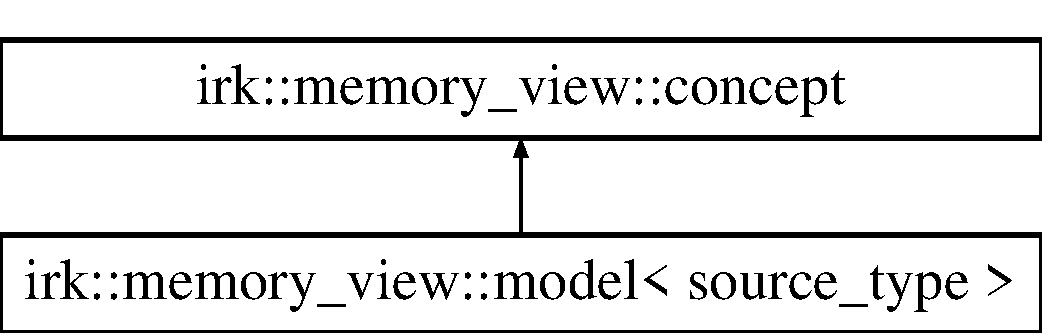
\includegraphics[height=2.000000cm]{classirk_1_1memory__view_1_1model}
\end{center}
\end{figure}
\subsection*{Public Member Functions}
\begin{DoxyCompactItemize}
\item 
\mbox{\hyperlink{classirk_1_1memory__view_1_1model_a47843c84f96ecb25ce8c81ce47c214b4}{model}} (\mbox{\hyperlink{irk-score_8cpp_a73f57f67fb1e33bdbfd80bfba2fc9ffe}{source\+\_\+type}} source)
\item 
const char $\ast$ \mbox{\hyperlink{classirk_1_1memory__view_1_1model_a5a7c432c460f99bd8b78c29ef6d44009}{data}} () const override
\item 
gsl\+::index \mbox{\hyperlink{classirk_1_1memory__view_1_1model_a88bdaaf00f71b733bb67ea912ed78251}{size}} () const override
\item 
const char \& \mbox{\hyperlink{classirk_1_1memory__view_1_1model_a8c54be09ffb8bd159e375d14a6f8218b}{operator\mbox{[}$\,$\mbox{]}}} (std\+::ptrdiff\+\_\+t n) const override
\item 
\mbox{\hyperlink{classirk_1_1memory__view}{memory\+\_\+view}} \mbox{\hyperlink{classirk_1_1memory__view_1_1model_aed67f637a1f0e7e31dcf039074861724}{range}} (std\+::ptrdiff\+\_\+t first, std\+::ptrdiff\+\_\+t \mbox{\hyperlink{classirk_1_1memory__view_1_1model_a88bdaaf00f71b733bb67ea912ed78251}{size}}) const override
\end{DoxyCompactItemize}


\subsection{Constructor \& Destructor Documentation}
\mbox{\Hypertarget{classirk_1_1memory__view_1_1model_a47843c84f96ecb25ce8c81ce47c214b4}\label{classirk_1_1memory__view_1_1model_a47843c84f96ecb25ce8c81ce47c214b4}} 
\index{irk\+::memory\+\_\+view\+::model@{irk\+::memory\+\_\+view\+::model}!model@{model}}
\index{model@{model}!irk\+::memory\+\_\+view\+::model@{irk\+::memory\+\_\+view\+::model}}
\subsubsection{\texorpdfstring{model()}{model()}}
{\footnotesize\ttfamily template$<$class source\+\_\+type $>$ \\
\mbox{\hyperlink{classirk_1_1memory__view_1_1model}{irk\+::memory\+\_\+view\+::model}}$<$ \mbox{\hyperlink{irk-score_8cpp_a73f57f67fb1e33bdbfd80bfba2fc9ffe}{source\+\_\+type}} $>$\+::\mbox{\hyperlink{classirk_1_1memory__view_1_1model}{model}} (\begin{DoxyParamCaption}\item[{\mbox{\hyperlink{irk-score_8cpp_a73f57f67fb1e33bdbfd80bfba2fc9ffe}{source\+\_\+type}}}]{source }\end{DoxyParamCaption})\hspace{0.3cm}{\ttfamily [inline]}, {\ttfamily [explicit]}}



\subsection{Member Function Documentation}
\mbox{\Hypertarget{classirk_1_1memory__view_1_1model_a5a7c432c460f99bd8b78c29ef6d44009}\label{classirk_1_1memory__view_1_1model_a5a7c432c460f99bd8b78c29ef6d44009}} 
\index{irk\+::memory\+\_\+view\+::model@{irk\+::memory\+\_\+view\+::model}!data@{data}}
\index{data@{data}!irk\+::memory\+\_\+view\+::model@{irk\+::memory\+\_\+view\+::model}}
\subsubsection{\texorpdfstring{data()}{data()}}
{\footnotesize\ttfamily template$<$class source\+\_\+type $>$ \\
const char$\ast$ \mbox{\hyperlink{classirk_1_1memory__view_1_1model}{irk\+::memory\+\_\+view\+::model}}$<$ \mbox{\hyperlink{irk-score_8cpp_a73f57f67fb1e33bdbfd80bfba2fc9ffe}{source\+\_\+type}} $>$\+::data (\begin{DoxyParamCaption}{ }\end{DoxyParamCaption}) const\hspace{0.3cm}{\ttfamily [inline]}, {\ttfamily [override]}, {\ttfamily [virtual]}}



Implements \mbox{\hyperlink{structirk_1_1memory__view_1_1concept_a9e124ac4016556f7cf7fd864dcc43a7c}{irk\+::memory\+\_\+view\+::concept}}.

\mbox{\Hypertarget{classirk_1_1memory__view_1_1model_a8c54be09ffb8bd159e375d14a6f8218b}\label{classirk_1_1memory__view_1_1model_a8c54be09ffb8bd159e375d14a6f8218b}} 
\index{irk\+::memory\+\_\+view\+::model@{irk\+::memory\+\_\+view\+::model}!operator\mbox{[}\mbox{]}@{operator[]}}
\index{operator\mbox{[}\mbox{]}@{operator[]}!irk\+::memory\+\_\+view\+::model@{irk\+::memory\+\_\+view\+::model}}
\subsubsection{\texorpdfstring{operator[]()}{operator[]()}}
{\footnotesize\ttfamily template$<$class source\+\_\+type $>$ \\
const char\& \mbox{\hyperlink{classirk_1_1memory__view_1_1model}{irk\+::memory\+\_\+view\+::model}}$<$ \mbox{\hyperlink{irk-score_8cpp_a73f57f67fb1e33bdbfd80bfba2fc9ffe}{source\+\_\+type}} $>$\+::operator\mbox{[}$\,$\mbox{]} (\begin{DoxyParamCaption}\item[{std\+::ptrdiff\+\_\+t}]{n }\end{DoxyParamCaption}) const\hspace{0.3cm}{\ttfamily [inline]}, {\ttfamily [override]}, {\ttfamily [virtual]}}



Implements \mbox{\hyperlink{structirk_1_1memory__view_1_1concept_af36b274207af910870d186a747b9f9f1}{irk\+::memory\+\_\+view\+::concept}}.

\mbox{\Hypertarget{classirk_1_1memory__view_1_1model_aed67f637a1f0e7e31dcf039074861724}\label{classirk_1_1memory__view_1_1model_aed67f637a1f0e7e31dcf039074861724}} 
\index{irk\+::memory\+\_\+view\+::model@{irk\+::memory\+\_\+view\+::model}!range@{range}}
\index{range@{range}!irk\+::memory\+\_\+view\+::model@{irk\+::memory\+\_\+view\+::model}}
\subsubsection{\texorpdfstring{range()}{range()}}
{\footnotesize\ttfamily template$<$class source\+\_\+type $>$ \\
\mbox{\hyperlink{classirk_1_1memory__view}{memory\+\_\+view}} \mbox{\hyperlink{classirk_1_1memory__view_1_1model}{irk\+::memory\+\_\+view\+::model}}$<$ \mbox{\hyperlink{irk-score_8cpp_a73f57f67fb1e33bdbfd80bfba2fc9ffe}{source\+\_\+type}} $>$\+::range (\begin{DoxyParamCaption}\item[{std\+::ptrdiff\+\_\+t}]{first,  }\item[{std\+::ptrdiff\+\_\+t}]{size }\end{DoxyParamCaption}) const\hspace{0.3cm}{\ttfamily [inline]}, {\ttfamily [override]}, {\ttfamily [virtual]}}



Implements \mbox{\hyperlink{structirk_1_1memory__view_1_1concept_a9abcd2995563487390e941cf502b322c}{irk\+::memory\+\_\+view\+::concept}}.

\mbox{\Hypertarget{classirk_1_1memory__view_1_1model_a88bdaaf00f71b733bb67ea912ed78251}\label{classirk_1_1memory__view_1_1model_a88bdaaf00f71b733bb67ea912ed78251}} 
\index{irk\+::memory\+\_\+view\+::model@{irk\+::memory\+\_\+view\+::model}!size@{size}}
\index{size@{size}!irk\+::memory\+\_\+view\+::model@{irk\+::memory\+\_\+view\+::model}}
\subsubsection{\texorpdfstring{size()}{size()}}
{\footnotesize\ttfamily template$<$class source\+\_\+type $>$ \\
gsl\+::index \mbox{\hyperlink{classirk_1_1memory__view_1_1model}{irk\+::memory\+\_\+view\+::model}}$<$ \mbox{\hyperlink{irk-score_8cpp_a73f57f67fb1e33bdbfd80bfba2fc9ffe}{source\+\_\+type}} $>$\+::size (\begin{DoxyParamCaption}{ }\end{DoxyParamCaption}) const\hspace{0.3cm}{\ttfamily [inline]}, {\ttfamily [override]}, {\ttfamily [virtual]}}



Implements \mbox{\hyperlink{structirk_1_1memory__view_1_1concept_ae280e124e776a61562f6a97b2fa7d655}{irk\+::memory\+\_\+view\+::concept}}.



The documentation for this class was generated from the following file\+:\begin{DoxyCompactItemize}
\item 
include/irkit/\mbox{\hyperlink{memoryview_8hpp}{memoryview.\+hpp}}\end{DoxyCompactItemize}

\hypertarget{structirk_1_1moving__range}{}\section{irk\+:\+:moving\+\_\+range$<$ Iter $>$ Struct Template Reference}
\label{structirk_1_1moving__range}\index{irk\+::moving\+\_\+range$<$ Iter $>$@{irk\+::moving\+\_\+range$<$ Iter $>$}}


A container for two ends of iterators.  




{\ttfamily \#include $<$movingrange.\+hpp$>$}

\subsection*{Public Types}
\begin{DoxyCompactItemize}
\item 
using \mbox{\hyperlink{structirk_1_1moving__range_ad77e99c581516edfaae4cdb3cc6793ba}{iterator\+\_\+type}} = Iter
\item 
using \mbox{\hyperlink{structirk_1_1moving__range_a53b63b6f5e9e758aab935274c09355de}{element\+\_\+type}} = decltype($\ast$std\+::declval$<$ Iter $>$())
\end{DoxyCompactItemize}
\subsection*{Public Member Functions}
\begin{DoxyCompactItemize}
\item 
\mbox{\hyperlink{structirk_1_1moving__range_a20e176576675bfd01b511fb250df1e5f}{moving\+\_\+range}} ()=default
\item 
\mbox{\hyperlink{structirk_1_1moving__range_a4db0c17a812a7562a87e749b7313a0c9}{moving\+\_\+range}} (\mbox{\hyperlink{structirk_1_1moving__range_ad77e99c581516edfaae4cdb3cc6793ba}{iterator\+\_\+type}} first, \mbox{\hyperlink{structirk_1_1moving__range_ad77e99c581516edfaae4cdb3cc6793ba}{iterator\+\_\+type}} last)
\item 
bool \mbox{\hyperlink{structirk_1_1moving__range_ae3f8227591a53d22d087d8633ce3172f}{empty}} () const
\item 
void \mbox{\hyperlink{structirk_1_1moving__range_ae842c24ac2957ac1f68bd3d22e251e47}{advance}} ()
\begin{DoxyCompactList}\small\item\em Advances the left end of the range by one. \end{DoxyCompactList}\item 
void \mbox{\hyperlink{structirk_1_1moving__range_ab184b9ac91013a6de5b31abef0498371}{advance}} (unsigned int n)
\begin{DoxyCompactList}\small\item\em Advances the left end of the range by {\ttfamily n}. \end{DoxyCompactList}\item 
\mbox{\hyperlink{structirk_1_1moving__range_ad77e99c581516edfaae4cdb3cc6793ba}{iterator\+\_\+type}} \mbox{\hyperlink{structirk_1_1moving__range_ac24e6010803fdad694992f2a677dfdbb}{begin}} () const
\item 
\mbox{\hyperlink{structirk_1_1moving__range_ad77e99c581516edfaae4cdb3cc6793ba}{iterator\+\_\+type}} \mbox{\hyperlink{structirk_1_1moving__range_ad904d898c5132ebb7d6f479db591d093}{end}} () const
\item 
auto \mbox{\hyperlink{structirk_1_1moving__range_a10d1586db8a0f1cca48e27ca0cc4b2a9}{front}} () const
\end{DoxyCompactItemize}
\subsection*{Public Attributes}
\begin{DoxyCompactItemize}
\item 
\mbox{\hyperlink{structirk_1_1moving__range_ad77e99c581516edfaae4cdb3cc6793ba}{iterator\+\_\+type}} \mbox{\hyperlink{structirk_1_1moving__range_a320ea432eef08a78898777273010d605}{left}}
\begin{DoxyCompactList}\small\item\em The left end of the range. \end{DoxyCompactList}\item 
\mbox{\hyperlink{structirk_1_1moving__range_ad77e99c581516edfaae4cdb3cc6793ba}{iterator\+\_\+type}} \mbox{\hyperlink{structirk_1_1moving__range_a60373930b24fd6f602d42cc06f129229}{right}}
\begin{DoxyCompactList}\small\item\em The right end of the range (after the last element). \end{DoxyCompactList}\end{DoxyCompactItemize}


\subsection{Detailed Description}
\subsubsection*{template$<$class Iter$>$\newline
struct irk\+::moving\+\_\+range$<$ Iter $>$}

A container for two ends of iterators. 

\begin{DoxyAuthor}{Author}
Michal Siedlaczek \href{http://github.com/elshize}{\tt http\+://github.\+com/elshize}
\end{DoxyAuthor}
T\+O\+DO\+:
\begin{DoxyItemize}
\item Needs to be generalized, for containers as well?
\item Implement iterator methods. 
\end{DoxyItemize}

\subsection{Member Typedef Documentation}
\mbox{\Hypertarget{structirk_1_1moving__range_a53b63b6f5e9e758aab935274c09355de}\label{structirk_1_1moving__range_a53b63b6f5e9e758aab935274c09355de}} 
\index{irk\+::moving\+\_\+range@{irk\+::moving\+\_\+range}!element\+\_\+type@{element\+\_\+type}}
\index{element\+\_\+type@{element\+\_\+type}!irk\+::moving\+\_\+range@{irk\+::moving\+\_\+range}}
\subsubsection{\texorpdfstring{element\+\_\+type}{element\_type}}
{\footnotesize\ttfamily template$<$class Iter $>$ \\
using \mbox{\hyperlink{structirk_1_1moving__range}{irk\+::moving\+\_\+range}}$<$ Iter $>$\+::\mbox{\hyperlink{structirk_1_1moving__range_a53b63b6f5e9e758aab935274c09355de}{element\+\_\+type}} =  decltype($\ast$std\+::declval$<$Iter$>$())}

\mbox{\Hypertarget{structirk_1_1moving__range_ad77e99c581516edfaae4cdb3cc6793ba}\label{structirk_1_1moving__range_ad77e99c581516edfaae4cdb3cc6793ba}} 
\index{irk\+::moving\+\_\+range@{irk\+::moving\+\_\+range}!iterator\+\_\+type@{iterator\+\_\+type}}
\index{iterator\+\_\+type@{iterator\+\_\+type}!irk\+::moving\+\_\+range@{irk\+::moving\+\_\+range}}
\subsubsection{\texorpdfstring{iterator\+\_\+type}{iterator\_type}}
{\footnotesize\ttfamily template$<$class Iter $>$ \\
using \mbox{\hyperlink{structirk_1_1moving__range}{irk\+::moving\+\_\+range}}$<$ Iter $>$\+::\mbox{\hyperlink{structirk_1_1moving__range_ad77e99c581516edfaae4cdb3cc6793ba}{iterator\+\_\+type}} =  Iter}



\subsection{Constructor \& Destructor Documentation}
\mbox{\Hypertarget{structirk_1_1moving__range_a20e176576675bfd01b511fb250df1e5f}\label{structirk_1_1moving__range_a20e176576675bfd01b511fb250df1e5f}} 
\index{irk\+::moving\+\_\+range@{irk\+::moving\+\_\+range}!moving\+\_\+range@{moving\+\_\+range}}
\index{moving\+\_\+range@{moving\+\_\+range}!irk\+::moving\+\_\+range@{irk\+::moving\+\_\+range}}
\subsubsection{\texorpdfstring{moving\+\_\+range()}{moving\_range()}\hspace{0.1cm}{\footnotesize\ttfamily [1/2]}}
{\footnotesize\ttfamily template$<$class Iter $>$ \\
\mbox{\hyperlink{structirk_1_1moving__range}{irk\+::moving\+\_\+range}}$<$ Iter $>$\+::\mbox{\hyperlink{structirk_1_1moving__range}{moving\+\_\+range}} (\begin{DoxyParamCaption}{ }\end{DoxyParamCaption})\hspace{0.3cm}{\ttfamily [default]}}

\mbox{\Hypertarget{structirk_1_1moving__range_a4db0c17a812a7562a87e749b7313a0c9}\label{structirk_1_1moving__range_a4db0c17a812a7562a87e749b7313a0c9}} 
\index{irk\+::moving\+\_\+range@{irk\+::moving\+\_\+range}!moving\+\_\+range@{moving\+\_\+range}}
\index{moving\+\_\+range@{moving\+\_\+range}!irk\+::moving\+\_\+range@{irk\+::moving\+\_\+range}}
\subsubsection{\texorpdfstring{moving\+\_\+range()}{moving\_range()}\hspace{0.1cm}{\footnotesize\ttfamily [2/2]}}
{\footnotesize\ttfamily template$<$class Iter $>$ \\
\mbox{\hyperlink{structirk_1_1moving__range}{irk\+::moving\+\_\+range}}$<$ Iter $>$\+::\mbox{\hyperlink{structirk_1_1moving__range}{moving\+\_\+range}} (\begin{DoxyParamCaption}\item[{\mbox{\hyperlink{structirk_1_1moving__range_ad77e99c581516edfaae4cdb3cc6793ba}{iterator\+\_\+type}}}]{first,  }\item[{\mbox{\hyperlink{structirk_1_1moving__range_ad77e99c581516edfaae4cdb3cc6793ba}{iterator\+\_\+type}}}]{last }\end{DoxyParamCaption})\hspace{0.3cm}{\ttfamily [inline]}}



\subsection{Member Function Documentation}
\mbox{\Hypertarget{structirk_1_1moving__range_ae842c24ac2957ac1f68bd3d22e251e47}\label{structirk_1_1moving__range_ae842c24ac2957ac1f68bd3d22e251e47}} 
\index{irk\+::moving\+\_\+range@{irk\+::moving\+\_\+range}!advance@{advance}}
\index{advance@{advance}!irk\+::moving\+\_\+range@{irk\+::moving\+\_\+range}}
\subsubsection{\texorpdfstring{advance()}{advance()}\hspace{0.1cm}{\footnotesize\ttfamily [1/2]}}
{\footnotesize\ttfamily template$<$class Iter $>$ \\
void \mbox{\hyperlink{structirk_1_1moving__range}{irk\+::moving\+\_\+range}}$<$ Iter $>$\+::advance (\begin{DoxyParamCaption}{ }\end{DoxyParamCaption})\hspace{0.3cm}{\ttfamily [inline]}}



Advances the left end of the range by one. 

\mbox{\Hypertarget{structirk_1_1moving__range_ab184b9ac91013a6de5b31abef0498371}\label{structirk_1_1moving__range_ab184b9ac91013a6de5b31abef0498371}} 
\index{irk\+::moving\+\_\+range@{irk\+::moving\+\_\+range}!advance@{advance}}
\index{advance@{advance}!irk\+::moving\+\_\+range@{irk\+::moving\+\_\+range}}
\subsubsection{\texorpdfstring{advance()}{advance()}\hspace{0.1cm}{\footnotesize\ttfamily [2/2]}}
{\footnotesize\ttfamily template$<$class Iter $>$ \\
void \mbox{\hyperlink{structirk_1_1moving__range}{irk\+::moving\+\_\+range}}$<$ Iter $>$\+::advance (\begin{DoxyParamCaption}\item[{unsigned int}]{n }\end{DoxyParamCaption})\hspace{0.3cm}{\ttfamily [inline]}}



Advances the left end of the range by {\ttfamily n}. 

\mbox{\Hypertarget{structirk_1_1moving__range_ac24e6010803fdad694992f2a677dfdbb}\label{structirk_1_1moving__range_ac24e6010803fdad694992f2a677dfdbb}} 
\index{irk\+::moving\+\_\+range@{irk\+::moving\+\_\+range}!begin@{begin}}
\index{begin@{begin}!irk\+::moving\+\_\+range@{irk\+::moving\+\_\+range}}
\subsubsection{\texorpdfstring{begin()}{begin()}}
{\footnotesize\ttfamily template$<$class Iter $>$ \\
\mbox{\hyperlink{structirk_1_1moving__range_ad77e99c581516edfaae4cdb3cc6793ba}{iterator\+\_\+type}} \mbox{\hyperlink{structirk_1_1moving__range}{irk\+::moving\+\_\+range}}$<$ Iter $>$\+::begin (\begin{DoxyParamCaption}{ }\end{DoxyParamCaption}) const\hspace{0.3cm}{\ttfamily [inline]}}

\mbox{\Hypertarget{structirk_1_1moving__range_ae3f8227591a53d22d087d8633ce3172f}\label{structirk_1_1moving__range_ae3f8227591a53d22d087d8633ce3172f}} 
\index{irk\+::moving\+\_\+range@{irk\+::moving\+\_\+range}!empty@{empty}}
\index{empty@{empty}!irk\+::moving\+\_\+range@{irk\+::moving\+\_\+range}}
\subsubsection{\texorpdfstring{empty()}{empty()}}
{\footnotesize\ttfamily template$<$class Iter $>$ \\
bool \mbox{\hyperlink{structirk_1_1moving__range}{irk\+::moving\+\_\+range}}$<$ Iter $>$\+::empty (\begin{DoxyParamCaption}{ }\end{DoxyParamCaption}) const\hspace{0.3cm}{\ttfamily [inline]}}

\mbox{\Hypertarget{structirk_1_1moving__range_ad904d898c5132ebb7d6f479db591d093}\label{structirk_1_1moving__range_ad904d898c5132ebb7d6f479db591d093}} 
\index{irk\+::moving\+\_\+range@{irk\+::moving\+\_\+range}!end@{end}}
\index{end@{end}!irk\+::moving\+\_\+range@{irk\+::moving\+\_\+range}}
\subsubsection{\texorpdfstring{end()}{end()}}
{\footnotesize\ttfamily template$<$class Iter $>$ \\
\mbox{\hyperlink{structirk_1_1moving__range_ad77e99c581516edfaae4cdb3cc6793ba}{iterator\+\_\+type}} \mbox{\hyperlink{structirk_1_1moving__range}{irk\+::moving\+\_\+range}}$<$ Iter $>$\+::end (\begin{DoxyParamCaption}{ }\end{DoxyParamCaption}) const\hspace{0.3cm}{\ttfamily [inline]}}

\mbox{\Hypertarget{structirk_1_1moving__range_a10d1586db8a0f1cca48e27ca0cc4b2a9}\label{structirk_1_1moving__range_a10d1586db8a0f1cca48e27ca0cc4b2a9}} 
\index{irk\+::moving\+\_\+range@{irk\+::moving\+\_\+range}!front@{front}}
\index{front@{front}!irk\+::moving\+\_\+range@{irk\+::moving\+\_\+range}}
\subsubsection{\texorpdfstring{front()}{front()}}
{\footnotesize\ttfamily template$<$class Iter $>$ \\
auto \mbox{\hyperlink{structirk_1_1moving__range}{irk\+::moving\+\_\+range}}$<$ Iter $>$\+::front (\begin{DoxyParamCaption}{ }\end{DoxyParamCaption}) const\hspace{0.3cm}{\ttfamily [inline]}}



\subsection{Member Data Documentation}
\mbox{\Hypertarget{structirk_1_1moving__range_a320ea432eef08a78898777273010d605}\label{structirk_1_1moving__range_a320ea432eef08a78898777273010d605}} 
\index{irk\+::moving\+\_\+range@{irk\+::moving\+\_\+range}!left@{left}}
\index{left@{left}!irk\+::moving\+\_\+range@{irk\+::moving\+\_\+range}}
\subsubsection{\texorpdfstring{left}{left}}
{\footnotesize\ttfamily template$<$class Iter $>$ \\
\mbox{\hyperlink{structirk_1_1moving__range_ad77e99c581516edfaae4cdb3cc6793ba}{iterator\+\_\+type}} \mbox{\hyperlink{structirk_1_1moving__range}{irk\+::moving\+\_\+range}}$<$ Iter $>$\+::left}



The left end of the range. 

\mbox{\Hypertarget{structirk_1_1moving__range_a60373930b24fd6f602d42cc06f129229}\label{structirk_1_1moving__range_a60373930b24fd6f602d42cc06f129229}} 
\index{irk\+::moving\+\_\+range@{irk\+::moving\+\_\+range}!right@{right}}
\index{right@{right}!irk\+::moving\+\_\+range@{irk\+::moving\+\_\+range}}
\subsubsection{\texorpdfstring{right}{right}}
{\footnotesize\ttfamily template$<$class Iter $>$ \\
\mbox{\hyperlink{structirk_1_1moving__range_ad77e99c581516edfaae4cdb3cc6793ba}{iterator\+\_\+type}} \mbox{\hyperlink{structirk_1_1moving__range}{irk\+::moving\+\_\+range}}$<$ Iter $>$\+::right}



The right end of the range (after the last element). 



The documentation for this struct was generated from the following file\+:\begin{DoxyCompactItemize}
\item 
include/irkit/\mbox{\hyperlink{movingrange_8hpp}{movingrange.\+hpp}}\end{DoxyCompactItemize}

\hypertarget{classirk_1_1mutable__bit__trie}{}\section{irk\+:\+:mutable\+\_\+bit\+\_\+trie$<$ Value $>$ Class Template Reference}
\label{classirk_1_1mutable__bit__trie}\index{irk\+::mutable\+\_\+bit\+\_\+trie$<$ Value $>$@{irk\+::mutable\+\_\+bit\+\_\+trie$<$ Value $>$}}


In-\/memory, mutable implementation of Bitwise Trie.  




{\ttfamily \#include $<$mutablebittrie.\+hpp$>$}

\subsection*{Classes}
\begin{DoxyCompactItemize}
\item 
struct \mbox{\hyperlink{structirk_1_1mutable__bit__trie_1_1node}{node}}
\end{DoxyCompactItemize}
\subsection*{Public Types}
\begin{DoxyCompactItemize}
\item 
using \mbox{\hyperlink{classirk_1_1mutable__bit__trie_abd23179ac4f02a981d4f47b4c0652287}{node\+\_\+ptr}} = std\+::shared\+\_\+ptr$<$ \mbox{\hyperlink{structirk_1_1mutable__bit__trie_1_1node}{node}} $>$
\item 
using \mbox{\hyperlink{classirk_1_1mutable__bit__trie_a9a5ed79af3e7e28054b00c2284b35612}{value\+\_\+opt}} = std\+::optional$<$ Value $>$
\end{DoxyCompactItemize}
\subsection*{Public Member Functions}
\begin{DoxyCompactItemize}
\item 
\mbox{\hyperlink{classirk_1_1mutable__bit__trie_a6927e834f866c053925d9ddf902774c1}{mutable\+\_\+bit\+\_\+trie}} ()
\item 
\mbox{\hyperlink{classirk_1_1mutable__bit__trie_a25fac71898d72afb04fc581ee5a913e7}{mutable\+\_\+bit\+\_\+trie}} (\mbox{\hyperlink{classirk_1_1mutable__bit__trie_abd23179ac4f02a981d4f47b4c0652287}{node\+\_\+ptr}} \mbox{\hyperlink{classirk_1_1mutable__bit__trie_a82b109eb8816a4ff9093ca5649d13db9}{root}})
\item 
\mbox{\hyperlink{classirk_1_1mutable__bit__trie_abd23179ac4f02a981d4f47b4c0652287}{node\+\_\+ptr}} \mbox{\hyperlink{classirk_1_1mutable__bit__trie_a82b109eb8816a4ff9093ca5649d13db9}{root}} () const
\item 
{\footnotesize template$<$class  = std\+::enable\+\_\+if\+\_\+t$<$std\+::is\+\_\+same$<$\+Value, void$>$\+::value$>$$>$ }\\bool \mbox{\hyperlink{classirk_1_1mutable__bit__trie_ab502e5df64f1e9fd767e2963f210334b}{insert}} (const \mbox{\hyperlink{namespaceirk_a979e09720c2ef05573819388a3c0e79a}{bitword}} \&encoded)
\item 
bool \mbox{\hyperlink{classirk_1_1mutable__bit__trie_a694f1825422ce94a786bc922baef651d}{insert}} (const \mbox{\hyperlink{namespaceirk_a979e09720c2ef05573819388a3c0e79a}{bitword}} \&encoded, Value \mbox{\hyperlink{classirk_1_1mutable__bit__trie_ad0bb2e18842b722d7deb1a5d4b72b890}{value}})
\item 
std\+::pair$<$ bool, \mbox{\hyperlink{classirk_1_1mutable__bit__trie_abd23179ac4f02a981d4f47b4c0652287}{node\+\_\+ptr}} $>$ \mbox{\hyperlink{classirk_1_1mutable__bit__trie_a30d25f61a4f6e7cb8d9ac6f0ff205f97}{find\+\_\+or\+\_\+first\+\_\+lower}} (const \mbox{\hyperlink{namespaceirk_a979e09720c2ef05573819388a3c0e79a}{bitword}} \&encoded) const
\item 
std\+::pair$<$ std\+::size\+\_\+t, \mbox{\hyperlink{classirk_1_1mutable__bit__trie_abd23179ac4f02a981d4f47b4c0652287}{node\+\_\+ptr}} $>$ \mbox{\hyperlink{classirk_1_1mutable__bit__trie_af0bd766c6c437fcdcb9612ba9de84510}{find}} (const \mbox{\hyperlink{namespaceirk_a979e09720c2ef05573819388a3c0e79a}{bitword}} \&encoded) const
\item 
bool \mbox{\hyperlink{classirk_1_1mutable__bit__trie_ab45e17c9d8b88f14654d52e27c092c30}{contains}} (const \mbox{\hyperlink{namespaceirk_a979e09720c2ef05573819388a3c0e79a}{bitword}} \&encoded) const
\item 
std\+::optional$<$ Value $>$ \mbox{\hyperlink{classirk_1_1mutable__bit__trie_ad0bb2e18842b722d7deb1a5d4b72b890}{value}} (const \mbox{\hyperlink{namespaceirk_a979e09720c2ef05573819388a3c0e79a}{bitword}} \&encoded) const
\item 
bool \mbox{\hyperlink{classirk_1_1mutable__bit__trie_abbfbe73cb98af4bb0375f00229cec50a}{empty}} () const
\end{DoxyCompactItemize}
\subsection*{Friends}
\begin{DoxyCompactItemize}
\item 
{\footnotesize template$<$class V $>$ }\\std\+::ostream \& \mbox{\hyperlink{classirk_1_1mutable__bit__trie_a91e672d5695fe80b17bbfd474d593ec2}{operator$<$$<$}} (std\+::ostream \&out, const \mbox{\hyperlink{classirk_1_1mutable__bit__trie}{mutable\+\_\+bit\+\_\+trie}}$<$ V $>$ \&mbt)
\end{DoxyCompactItemize}


\subsection{Detailed Description}
\subsubsection*{template$<$class Value = bool$>$\newline
class irk\+::mutable\+\_\+bit\+\_\+trie$<$ Value $>$}

In-\/memory, mutable implementation of Bitwise Trie. 

This implementation is not optimized for efficiency (doesn\textquotesingle{}t necessarily mean it isn\textquotesingle{}t for most applications). Instead, it is meant to be used mainly for building tries, or whenever a mutable version is needed.

In particular, this implementation is not conservative when it comes to memory usage. Ease of use is a priority here. 

\subsection{Member Typedef Documentation}
\mbox{\Hypertarget{classirk_1_1mutable__bit__trie_abd23179ac4f02a981d4f47b4c0652287}\label{classirk_1_1mutable__bit__trie_abd23179ac4f02a981d4f47b4c0652287}} 
\index{irk\+::mutable\+\_\+bit\+\_\+trie@{irk\+::mutable\+\_\+bit\+\_\+trie}!node\+\_\+ptr@{node\+\_\+ptr}}
\index{node\+\_\+ptr@{node\+\_\+ptr}!irk\+::mutable\+\_\+bit\+\_\+trie@{irk\+::mutable\+\_\+bit\+\_\+trie}}
\subsubsection{\texorpdfstring{node\+\_\+ptr}{node\_ptr}}
{\footnotesize\ttfamily template$<$class Value = bool$>$ \\
using \mbox{\hyperlink{classirk_1_1mutable__bit__trie}{irk\+::mutable\+\_\+bit\+\_\+trie}}$<$ Value $>$\+::\mbox{\hyperlink{classirk_1_1mutable__bit__trie_abd23179ac4f02a981d4f47b4c0652287}{node\+\_\+ptr}} =  std\+::shared\+\_\+ptr$<$\mbox{\hyperlink{structirk_1_1mutable__bit__trie_1_1node}{node}}$>$}

\mbox{\Hypertarget{classirk_1_1mutable__bit__trie_a9a5ed79af3e7e28054b00c2284b35612}\label{classirk_1_1mutable__bit__trie_a9a5ed79af3e7e28054b00c2284b35612}} 
\index{irk\+::mutable\+\_\+bit\+\_\+trie@{irk\+::mutable\+\_\+bit\+\_\+trie}!value\+\_\+opt@{value\+\_\+opt}}
\index{value\+\_\+opt@{value\+\_\+opt}!irk\+::mutable\+\_\+bit\+\_\+trie@{irk\+::mutable\+\_\+bit\+\_\+trie}}
\subsubsection{\texorpdfstring{value\+\_\+opt}{value\_opt}}
{\footnotesize\ttfamily template$<$class Value = bool$>$ \\
using \mbox{\hyperlink{classirk_1_1mutable__bit__trie}{irk\+::mutable\+\_\+bit\+\_\+trie}}$<$ Value $>$\+::\mbox{\hyperlink{classirk_1_1mutable__bit__trie_a9a5ed79af3e7e28054b00c2284b35612}{value\+\_\+opt}} =  std\+::optional$<$Value$>$}



\subsection{Constructor \& Destructor Documentation}
\mbox{\Hypertarget{classirk_1_1mutable__bit__trie_a6927e834f866c053925d9ddf902774c1}\label{classirk_1_1mutable__bit__trie_a6927e834f866c053925d9ddf902774c1}} 
\index{irk\+::mutable\+\_\+bit\+\_\+trie@{irk\+::mutable\+\_\+bit\+\_\+trie}!mutable\+\_\+bit\+\_\+trie@{mutable\+\_\+bit\+\_\+trie}}
\index{mutable\+\_\+bit\+\_\+trie@{mutable\+\_\+bit\+\_\+trie}!irk\+::mutable\+\_\+bit\+\_\+trie@{irk\+::mutable\+\_\+bit\+\_\+trie}}
\subsubsection{\texorpdfstring{mutable\+\_\+bit\+\_\+trie()}{mutable\_bit\_trie()}\hspace{0.1cm}{\footnotesize\ttfamily [1/2]}}
{\footnotesize\ttfamily template$<$class Value = bool$>$ \\
\mbox{\hyperlink{classirk_1_1mutable__bit__trie}{irk\+::mutable\+\_\+bit\+\_\+trie}}$<$ Value $>$\+::\mbox{\hyperlink{classirk_1_1mutable__bit__trie}{mutable\+\_\+bit\+\_\+trie}} (\begin{DoxyParamCaption}{ }\end{DoxyParamCaption})\hspace{0.3cm}{\ttfamily [inline]}}

\mbox{\Hypertarget{classirk_1_1mutable__bit__trie_a25fac71898d72afb04fc581ee5a913e7}\label{classirk_1_1mutable__bit__trie_a25fac71898d72afb04fc581ee5a913e7}} 
\index{irk\+::mutable\+\_\+bit\+\_\+trie@{irk\+::mutable\+\_\+bit\+\_\+trie}!mutable\+\_\+bit\+\_\+trie@{mutable\+\_\+bit\+\_\+trie}}
\index{mutable\+\_\+bit\+\_\+trie@{mutable\+\_\+bit\+\_\+trie}!irk\+::mutable\+\_\+bit\+\_\+trie@{irk\+::mutable\+\_\+bit\+\_\+trie}}
\subsubsection{\texorpdfstring{mutable\+\_\+bit\+\_\+trie()}{mutable\_bit\_trie()}\hspace{0.1cm}{\footnotesize\ttfamily [2/2]}}
{\footnotesize\ttfamily template$<$class Value = bool$>$ \\
\mbox{\hyperlink{classirk_1_1mutable__bit__trie}{irk\+::mutable\+\_\+bit\+\_\+trie}}$<$ Value $>$\+::\mbox{\hyperlink{classirk_1_1mutable__bit__trie}{mutable\+\_\+bit\+\_\+trie}} (\begin{DoxyParamCaption}\item[{\mbox{\hyperlink{classirk_1_1mutable__bit__trie_abd23179ac4f02a981d4f47b4c0652287}{node\+\_\+ptr}}}]{root }\end{DoxyParamCaption})\hspace{0.3cm}{\ttfamily [inline]}}



\subsection{Member Function Documentation}
\mbox{\Hypertarget{classirk_1_1mutable__bit__trie_ab45e17c9d8b88f14654d52e27c092c30}\label{classirk_1_1mutable__bit__trie_ab45e17c9d8b88f14654d52e27c092c30}} 
\index{irk\+::mutable\+\_\+bit\+\_\+trie@{irk\+::mutable\+\_\+bit\+\_\+trie}!contains@{contains}}
\index{contains@{contains}!irk\+::mutable\+\_\+bit\+\_\+trie@{irk\+::mutable\+\_\+bit\+\_\+trie}}
\subsubsection{\texorpdfstring{contains()}{contains()}}
{\footnotesize\ttfamily template$<$class Value = bool$>$ \\
bool \mbox{\hyperlink{classirk_1_1mutable__bit__trie}{irk\+::mutable\+\_\+bit\+\_\+trie}}$<$ Value $>$\+::contains (\begin{DoxyParamCaption}\item[{const \mbox{\hyperlink{namespaceirk_a979e09720c2ef05573819388a3c0e79a}{bitword}} \&}]{encoded }\end{DoxyParamCaption}) const\hspace{0.3cm}{\ttfamily [inline]}}

\mbox{\Hypertarget{classirk_1_1mutable__bit__trie_abbfbe73cb98af4bb0375f00229cec50a}\label{classirk_1_1mutable__bit__trie_abbfbe73cb98af4bb0375f00229cec50a}} 
\index{irk\+::mutable\+\_\+bit\+\_\+trie@{irk\+::mutable\+\_\+bit\+\_\+trie}!empty@{empty}}
\index{empty@{empty}!irk\+::mutable\+\_\+bit\+\_\+trie@{irk\+::mutable\+\_\+bit\+\_\+trie}}
\subsubsection{\texorpdfstring{empty()}{empty()}}
{\footnotesize\ttfamily template$<$class Value = bool$>$ \\
bool \mbox{\hyperlink{classirk_1_1mutable__bit__trie}{irk\+::mutable\+\_\+bit\+\_\+trie}}$<$ Value $>$\+::empty (\begin{DoxyParamCaption}{ }\end{DoxyParamCaption}) const\hspace{0.3cm}{\ttfamily [inline]}}

\mbox{\Hypertarget{classirk_1_1mutable__bit__trie_af0bd766c6c437fcdcb9612ba9de84510}\label{classirk_1_1mutable__bit__trie_af0bd766c6c437fcdcb9612ba9de84510}} 
\index{irk\+::mutable\+\_\+bit\+\_\+trie@{irk\+::mutable\+\_\+bit\+\_\+trie}!find@{find}}
\index{find@{find}!irk\+::mutable\+\_\+bit\+\_\+trie@{irk\+::mutable\+\_\+bit\+\_\+trie}}
\subsubsection{\texorpdfstring{find()}{find()}}
{\footnotesize\ttfamily template$<$class Value = bool$>$ \\
std\+::pair$<$std\+::size\+\_\+t, \mbox{\hyperlink{classirk_1_1mutable__bit__trie_abd23179ac4f02a981d4f47b4c0652287}{node\+\_\+ptr}}$>$ \mbox{\hyperlink{classirk_1_1mutable__bit__trie}{irk\+::mutable\+\_\+bit\+\_\+trie}}$<$ Value $>$\+::find (\begin{DoxyParamCaption}\item[{const \mbox{\hyperlink{namespaceirk_a979e09720c2ef05573819388a3c0e79a}{bitword}} \&}]{encoded }\end{DoxyParamCaption}) const\hspace{0.3cm}{\ttfamily [inline]}}

\mbox{\Hypertarget{classirk_1_1mutable__bit__trie_a30d25f61a4f6e7cb8d9ac6f0ff205f97}\label{classirk_1_1mutable__bit__trie_a30d25f61a4f6e7cb8d9ac6f0ff205f97}} 
\index{irk\+::mutable\+\_\+bit\+\_\+trie@{irk\+::mutable\+\_\+bit\+\_\+trie}!find\+\_\+or\+\_\+first\+\_\+lower@{find\+\_\+or\+\_\+first\+\_\+lower}}
\index{find\+\_\+or\+\_\+first\+\_\+lower@{find\+\_\+or\+\_\+first\+\_\+lower}!irk\+::mutable\+\_\+bit\+\_\+trie@{irk\+::mutable\+\_\+bit\+\_\+trie}}
\subsubsection{\texorpdfstring{find\+\_\+or\+\_\+first\+\_\+lower()}{find\_or\_first\_lower()}}
{\footnotesize\ttfamily template$<$class Value = bool$>$ \\
std\+::pair$<$bool, \mbox{\hyperlink{classirk_1_1mutable__bit__trie_abd23179ac4f02a981d4f47b4c0652287}{node\+\_\+ptr}}$>$ \mbox{\hyperlink{classirk_1_1mutable__bit__trie}{irk\+::mutable\+\_\+bit\+\_\+trie}}$<$ Value $>$\+::find\+\_\+or\+\_\+first\+\_\+lower (\begin{DoxyParamCaption}\item[{const \mbox{\hyperlink{namespaceirk_a979e09720c2ef05573819388a3c0e79a}{bitword}} \&}]{encoded }\end{DoxyParamCaption}) const\hspace{0.3cm}{\ttfamily [inline]}}

\mbox{\Hypertarget{classirk_1_1mutable__bit__trie_ab502e5df64f1e9fd767e2963f210334b}\label{classirk_1_1mutable__bit__trie_ab502e5df64f1e9fd767e2963f210334b}} 
\index{irk\+::mutable\+\_\+bit\+\_\+trie@{irk\+::mutable\+\_\+bit\+\_\+trie}!insert@{insert}}
\index{insert@{insert}!irk\+::mutable\+\_\+bit\+\_\+trie@{irk\+::mutable\+\_\+bit\+\_\+trie}}
\subsubsection{\texorpdfstring{insert()}{insert()}\hspace{0.1cm}{\footnotesize\ttfamily [1/2]}}
{\footnotesize\ttfamily template$<$class Value = bool$>$ \\
template$<$class  = std\+::enable\+\_\+if\+\_\+t$<$std\+::is\+\_\+same$<$\+Value, void$>$\+::value$>$$>$ \\
bool \mbox{\hyperlink{classirk_1_1mutable__bit__trie}{irk\+::mutable\+\_\+bit\+\_\+trie}}$<$ Value $>$\+::insert (\begin{DoxyParamCaption}\item[{const \mbox{\hyperlink{namespaceirk_a979e09720c2ef05573819388a3c0e79a}{bitword}} \&}]{encoded }\end{DoxyParamCaption})\hspace{0.3cm}{\ttfamily [inline]}}

\mbox{\Hypertarget{classirk_1_1mutable__bit__trie_a694f1825422ce94a786bc922baef651d}\label{classirk_1_1mutable__bit__trie_a694f1825422ce94a786bc922baef651d}} 
\index{irk\+::mutable\+\_\+bit\+\_\+trie@{irk\+::mutable\+\_\+bit\+\_\+trie}!insert@{insert}}
\index{insert@{insert}!irk\+::mutable\+\_\+bit\+\_\+trie@{irk\+::mutable\+\_\+bit\+\_\+trie}}
\subsubsection{\texorpdfstring{insert()}{insert()}\hspace{0.1cm}{\footnotesize\ttfamily [2/2]}}
{\footnotesize\ttfamily template$<$class Value = bool$>$ \\
bool \mbox{\hyperlink{classirk_1_1mutable__bit__trie}{irk\+::mutable\+\_\+bit\+\_\+trie}}$<$ Value $>$\+::insert (\begin{DoxyParamCaption}\item[{const \mbox{\hyperlink{namespaceirk_a979e09720c2ef05573819388a3c0e79a}{bitword}} \&}]{encoded,  }\item[{Value}]{value }\end{DoxyParamCaption})\hspace{0.3cm}{\ttfamily [inline]}}

\mbox{\Hypertarget{classirk_1_1mutable__bit__trie_a82b109eb8816a4ff9093ca5649d13db9}\label{classirk_1_1mutable__bit__trie_a82b109eb8816a4ff9093ca5649d13db9}} 
\index{irk\+::mutable\+\_\+bit\+\_\+trie@{irk\+::mutable\+\_\+bit\+\_\+trie}!root@{root}}
\index{root@{root}!irk\+::mutable\+\_\+bit\+\_\+trie@{irk\+::mutable\+\_\+bit\+\_\+trie}}
\subsubsection{\texorpdfstring{root()}{root()}}
{\footnotesize\ttfamily template$<$class Value = bool$>$ \\
\mbox{\hyperlink{classirk_1_1mutable__bit__trie_abd23179ac4f02a981d4f47b4c0652287}{node\+\_\+ptr}} \mbox{\hyperlink{classirk_1_1mutable__bit__trie}{irk\+::mutable\+\_\+bit\+\_\+trie}}$<$ Value $>$\+::root (\begin{DoxyParamCaption}{ }\end{DoxyParamCaption}) const\hspace{0.3cm}{\ttfamily [inline]}}

\mbox{\Hypertarget{classirk_1_1mutable__bit__trie_ad0bb2e18842b722d7deb1a5d4b72b890}\label{classirk_1_1mutable__bit__trie_ad0bb2e18842b722d7deb1a5d4b72b890}} 
\index{irk\+::mutable\+\_\+bit\+\_\+trie@{irk\+::mutable\+\_\+bit\+\_\+trie}!value@{value}}
\index{value@{value}!irk\+::mutable\+\_\+bit\+\_\+trie@{irk\+::mutable\+\_\+bit\+\_\+trie}}
\subsubsection{\texorpdfstring{value()}{value()}}
{\footnotesize\ttfamily template$<$class Value = bool$>$ \\
std\+::optional$<$Value$>$ \mbox{\hyperlink{classirk_1_1mutable__bit__trie}{irk\+::mutable\+\_\+bit\+\_\+trie}}$<$ Value $>$\+::value (\begin{DoxyParamCaption}\item[{const \mbox{\hyperlink{namespaceirk_a979e09720c2ef05573819388a3c0e79a}{bitword}} \&}]{encoded }\end{DoxyParamCaption}) const\hspace{0.3cm}{\ttfamily [inline]}}



\subsection{Friends And Related Function Documentation}
\mbox{\Hypertarget{classirk_1_1mutable__bit__trie_a91e672d5695fe80b17bbfd474d593ec2}\label{classirk_1_1mutable__bit__trie_a91e672d5695fe80b17bbfd474d593ec2}} 
\index{irk\+::mutable\+\_\+bit\+\_\+trie@{irk\+::mutable\+\_\+bit\+\_\+trie}!operator$<$$<$@{operator$<$$<$}}
\index{operator$<$$<$@{operator$<$$<$}!irk\+::mutable\+\_\+bit\+\_\+trie@{irk\+::mutable\+\_\+bit\+\_\+trie}}
\subsubsection{\texorpdfstring{operator$<$$<$}{operator<<}}
{\footnotesize\ttfamily template$<$class Value = bool$>$ \\
template$<$class V $>$ \\
std\+::ostream\& operator$<$$<$ (\begin{DoxyParamCaption}\item[{std\+::ostream \&}]{out,  }\item[{const \mbox{\hyperlink{classirk_1_1mutable__bit__trie}{mutable\+\_\+bit\+\_\+trie}}$<$ V $>$ \&}]{mbt }\end{DoxyParamCaption})\hspace{0.3cm}{\ttfamily [friend]}}



The documentation for this class was generated from the following file\+:\begin{DoxyCompactItemize}
\item 
include/irkit/\mbox{\hyperlink{mutablebittrie_8hpp}{mutablebittrie.\+hpp}}\end{DoxyCompactItemize}

\hypertarget{structirk_1_1no__weight}{}\section{irk\+:\+:no\+\_\+weight Struct Reference}
\label{structirk_1_1no__weight}\index{irk\+::no\+\_\+weight@{irk\+::no\+\_\+weight}}


A dummy weight type that does not change the score when multiplied.  




{\ttfamily \#include $<$taat.\+hpp$>$}



\subsection{Detailed Description}
A dummy weight type that does not change the score when multiplied. 

The documentation for this struct was generated from the following file\+:\begin{DoxyCompactItemize}
\item 
include/irkit/\mbox{\hyperlink{taat_8hpp}{taat.\+hpp}}\end{DoxyCompactItemize}

\hypertarget{structirk_1_1mutable__bit__trie_1_1node}{}\section{irk\+:\+:mutable\+\_\+bit\+\_\+trie$<$ Value $>$\+:\+:node Struct Reference}
\label{structirk_1_1mutable__bit__trie_1_1node}\index{irk\+::mutable\+\_\+bit\+\_\+trie$<$ Value $>$\+::node@{irk\+::mutable\+\_\+bit\+\_\+trie$<$ Value $>$\+::node}}


{\ttfamily \#include $<$mutablebittrie.\+hpp$>$}

\subsection*{Public Member Functions}
\begin{DoxyCompactItemize}
\item 
\mbox{\hyperlink{structirk_1_1mutable__bit__trie_1_1node_a74037ab76023b8ff9c1cd88f91d06684}{node}} (\mbox{\hyperlink{classirk_1_1mutable__bit__trie_abd23179ac4f02a981d4f47b4c0652287}{node\+\_\+ptr}} \mbox{\hyperlink{structirk_1_1mutable__bit__trie_1_1node_af59565476fb0ce3e3e3d57edbd8ca1de}{left}}=nullptr, \mbox{\hyperlink{classirk_1_1mutable__bit__trie_abd23179ac4f02a981d4f47b4c0652287}{node\+\_\+ptr}} \mbox{\hyperlink{structirk_1_1mutable__bit__trie_1_1node_ad75512c087c6adaf342b9c62fd115f55}{right}}=nullptr, \mbox{\hyperlink{classirk_1_1mutable__bit__trie_a9a5ed79af3e7e28054b00c2284b35612}{value\+\_\+opt}} \mbox{\hyperlink{structirk_1_1mutable__bit__trie_1_1node_a1bacc998d6276431578e9ecb8f3dfa59}{value}}=std\+::nullopt)
\item 
\mbox{\hyperlink{structirk_1_1mutable__bit__trie_1_1node_a8b89d07cbc5be62f39eb3995659812b2}{node}} (\mbox{\hyperlink{namespaceirk_a979e09720c2ef05573819388a3c0e79a}{bitword}} \mbox{\hyperlink{structirk_1_1mutable__bit__trie_1_1node_a8b55d968fa4274a91a6395ea1b9785a8}{bits}}, \mbox{\hyperlink{classirk_1_1mutable__bit__trie_abd23179ac4f02a981d4f47b4c0652287}{node\+\_\+ptr}} \mbox{\hyperlink{structirk_1_1mutable__bit__trie_1_1node_af59565476fb0ce3e3e3d57edbd8ca1de}{left}}=nullptr, \mbox{\hyperlink{classirk_1_1mutable__bit__trie_abd23179ac4f02a981d4f47b4c0652287}{node\+\_\+ptr}} \mbox{\hyperlink{structirk_1_1mutable__bit__trie_1_1node_ad75512c087c6adaf342b9c62fd115f55}{right}}=nullptr, \mbox{\hyperlink{classirk_1_1mutable__bit__trie_a9a5ed79af3e7e28054b00c2284b35612}{value\+\_\+opt}} \mbox{\hyperlink{structirk_1_1mutable__bit__trie_1_1node_a1bacc998d6276431578e9ecb8f3dfa59}{value}}=std\+::nullopt)
\item 
bool \mbox{\hyperlink{structirk_1_1mutable__bit__trie_1_1node_a3b28e6bf24b4500b5b9fd7d3c1bb48e0}{compressed}} () const
\end{DoxyCompactItemize}
\subsection*{Public Attributes}
\begin{DoxyCompactItemize}
\item 
\mbox{\hyperlink{namespaceirk_a979e09720c2ef05573819388a3c0e79a}{bitword}} \mbox{\hyperlink{structirk_1_1mutable__bit__trie_1_1node_a8b55d968fa4274a91a6395ea1b9785a8}{bits}}
\item 
\mbox{\hyperlink{classirk_1_1mutable__bit__trie_abd23179ac4f02a981d4f47b4c0652287}{node\+\_\+ptr}} \mbox{\hyperlink{structirk_1_1mutable__bit__trie_1_1node_af59565476fb0ce3e3e3d57edbd8ca1de}{left}}
\item 
\mbox{\hyperlink{classirk_1_1mutable__bit__trie_abd23179ac4f02a981d4f47b4c0652287}{node\+\_\+ptr}} \mbox{\hyperlink{structirk_1_1mutable__bit__trie_1_1node_ad75512c087c6adaf342b9c62fd115f55}{right}}
\item 
bool \mbox{\hyperlink{structirk_1_1mutable__bit__trie_1_1node_a54f76adb0cab3a380ba75cc039065e4d}{sentinel}}
\item 
\mbox{\hyperlink{classirk_1_1mutable__bit__trie_a9a5ed79af3e7e28054b00c2284b35612}{value\+\_\+opt}} \mbox{\hyperlink{structirk_1_1mutable__bit__trie_1_1node_a1bacc998d6276431578e9ecb8f3dfa59}{value}}
\end{DoxyCompactItemize}


\subsection{Constructor \& Destructor Documentation}
\mbox{\Hypertarget{structirk_1_1mutable__bit__trie_1_1node_a74037ab76023b8ff9c1cd88f91d06684}\label{structirk_1_1mutable__bit__trie_1_1node_a74037ab76023b8ff9c1cd88f91d06684}} 
\index{irk\+::mutable\+\_\+bit\+\_\+trie\+::node@{irk\+::mutable\+\_\+bit\+\_\+trie\+::node}!node@{node}}
\index{node@{node}!irk\+::mutable\+\_\+bit\+\_\+trie\+::node@{irk\+::mutable\+\_\+bit\+\_\+trie\+::node}}
\subsubsection{\texorpdfstring{node()}{node()}\hspace{0.1cm}{\footnotesize\ttfamily [1/2]}}
{\footnotesize\ttfamily template$<$class Value = bool$>$ \\
\mbox{\hyperlink{classirk_1_1mutable__bit__trie}{irk\+::mutable\+\_\+bit\+\_\+trie}}$<$ Value $>$\+::node\+::node (\begin{DoxyParamCaption}\item[{\mbox{\hyperlink{classirk_1_1mutable__bit__trie_abd23179ac4f02a981d4f47b4c0652287}{node\+\_\+ptr}}}]{left = {\ttfamily nullptr},  }\item[{\mbox{\hyperlink{classirk_1_1mutable__bit__trie_abd23179ac4f02a981d4f47b4c0652287}{node\+\_\+ptr}}}]{right = {\ttfamily nullptr},  }\item[{\mbox{\hyperlink{classirk_1_1mutable__bit__trie_a9a5ed79af3e7e28054b00c2284b35612}{value\+\_\+opt}}}]{value = {\ttfamily std\+:\+:nullopt} }\end{DoxyParamCaption})\hspace{0.3cm}{\ttfamily [inline]}}

\mbox{\Hypertarget{structirk_1_1mutable__bit__trie_1_1node_a8b89d07cbc5be62f39eb3995659812b2}\label{structirk_1_1mutable__bit__trie_1_1node_a8b89d07cbc5be62f39eb3995659812b2}} 
\index{irk\+::mutable\+\_\+bit\+\_\+trie\+::node@{irk\+::mutable\+\_\+bit\+\_\+trie\+::node}!node@{node}}
\index{node@{node}!irk\+::mutable\+\_\+bit\+\_\+trie\+::node@{irk\+::mutable\+\_\+bit\+\_\+trie\+::node}}
\subsubsection{\texorpdfstring{node()}{node()}\hspace{0.1cm}{\footnotesize\ttfamily [2/2]}}
{\footnotesize\ttfamily template$<$class Value = bool$>$ \\
\mbox{\hyperlink{classirk_1_1mutable__bit__trie}{irk\+::mutable\+\_\+bit\+\_\+trie}}$<$ Value $>$\+::node\+::node (\begin{DoxyParamCaption}\item[{\mbox{\hyperlink{namespaceirk_a979e09720c2ef05573819388a3c0e79a}{bitword}}}]{bits,  }\item[{\mbox{\hyperlink{classirk_1_1mutable__bit__trie_abd23179ac4f02a981d4f47b4c0652287}{node\+\_\+ptr}}}]{left = {\ttfamily nullptr},  }\item[{\mbox{\hyperlink{classirk_1_1mutable__bit__trie_abd23179ac4f02a981d4f47b4c0652287}{node\+\_\+ptr}}}]{right = {\ttfamily nullptr},  }\item[{\mbox{\hyperlink{classirk_1_1mutable__bit__trie_a9a5ed79af3e7e28054b00c2284b35612}{value\+\_\+opt}}}]{value = {\ttfamily std\+:\+:nullopt} }\end{DoxyParamCaption})\hspace{0.3cm}{\ttfamily [inline]}}



\subsection{Member Function Documentation}
\mbox{\Hypertarget{structirk_1_1mutable__bit__trie_1_1node_a3b28e6bf24b4500b5b9fd7d3c1bb48e0}\label{structirk_1_1mutable__bit__trie_1_1node_a3b28e6bf24b4500b5b9fd7d3c1bb48e0}} 
\index{irk\+::mutable\+\_\+bit\+\_\+trie\+::node@{irk\+::mutable\+\_\+bit\+\_\+trie\+::node}!compressed@{compressed}}
\index{compressed@{compressed}!irk\+::mutable\+\_\+bit\+\_\+trie\+::node@{irk\+::mutable\+\_\+bit\+\_\+trie\+::node}}
\subsubsection{\texorpdfstring{compressed()}{compressed()}}
{\footnotesize\ttfamily template$<$class Value = bool$>$ \\
bool \mbox{\hyperlink{classirk_1_1mutable__bit__trie}{irk\+::mutable\+\_\+bit\+\_\+trie}}$<$ Value $>$\+::node\+::compressed (\begin{DoxyParamCaption}{ }\end{DoxyParamCaption}) const\hspace{0.3cm}{\ttfamily [inline]}}



\subsection{Member Data Documentation}
\mbox{\Hypertarget{structirk_1_1mutable__bit__trie_1_1node_a8b55d968fa4274a91a6395ea1b9785a8}\label{structirk_1_1mutable__bit__trie_1_1node_a8b55d968fa4274a91a6395ea1b9785a8}} 
\index{irk\+::mutable\+\_\+bit\+\_\+trie\+::node@{irk\+::mutable\+\_\+bit\+\_\+trie\+::node}!bits@{bits}}
\index{bits@{bits}!irk\+::mutable\+\_\+bit\+\_\+trie\+::node@{irk\+::mutable\+\_\+bit\+\_\+trie\+::node}}
\subsubsection{\texorpdfstring{bits}{bits}}
{\footnotesize\ttfamily template$<$class Value = bool$>$ \\
\mbox{\hyperlink{namespaceirk_a979e09720c2ef05573819388a3c0e79a}{bitword}} \mbox{\hyperlink{classirk_1_1mutable__bit__trie}{irk\+::mutable\+\_\+bit\+\_\+trie}}$<$ Value $>$\+::node\+::bits}

\mbox{\Hypertarget{structirk_1_1mutable__bit__trie_1_1node_af59565476fb0ce3e3e3d57edbd8ca1de}\label{structirk_1_1mutable__bit__trie_1_1node_af59565476fb0ce3e3e3d57edbd8ca1de}} 
\index{irk\+::mutable\+\_\+bit\+\_\+trie\+::node@{irk\+::mutable\+\_\+bit\+\_\+trie\+::node}!left@{left}}
\index{left@{left}!irk\+::mutable\+\_\+bit\+\_\+trie\+::node@{irk\+::mutable\+\_\+bit\+\_\+trie\+::node}}
\subsubsection{\texorpdfstring{left}{left}}
{\footnotesize\ttfamily template$<$class Value = bool$>$ \\
\mbox{\hyperlink{classirk_1_1mutable__bit__trie_abd23179ac4f02a981d4f47b4c0652287}{node\+\_\+ptr}} \mbox{\hyperlink{classirk_1_1mutable__bit__trie}{irk\+::mutable\+\_\+bit\+\_\+trie}}$<$ Value $>$\+::node\+::left}

\mbox{\Hypertarget{structirk_1_1mutable__bit__trie_1_1node_ad75512c087c6adaf342b9c62fd115f55}\label{structirk_1_1mutable__bit__trie_1_1node_ad75512c087c6adaf342b9c62fd115f55}} 
\index{irk\+::mutable\+\_\+bit\+\_\+trie\+::node@{irk\+::mutable\+\_\+bit\+\_\+trie\+::node}!right@{right}}
\index{right@{right}!irk\+::mutable\+\_\+bit\+\_\+trie\+::node@{irk\+::mutable\+\_\+bit\+\_\+trie\+::node}}
\subsubsection{\texorpdfstring{right}{right}}
{\footnotesize\ttfamily template$<$class Value = bool$>$ \\
\mbox{\hyperlink{classirk_1_1mutable__bit__trie_abd23179ac4f02a981d4f47b4c0652287}{node\+\_\+ptr}} \mbox{\hyperlink{classirk_1_1mutable__bit__trie}{irk\+::mutable\+\_\+bit\+\_\+trie}}$<$ Value $>$\+::node\+::right}

\mbox{\Hypertarget{structirk_1_1mutable__bit__trie_1_1node_a54f76adb0cab3a380ba75cc039065e4d}\label{structirk_1_1mutable__bit__trie_1_1node_a54f76adb0cab3a380ba75cc039065e4d}} 
\index{irk\+::mutable\+\_\+bit\+\_\+trie\+::node@{irk\+::mutable\+\_\+bit\+\_\+trie\+::node}!sentinel@{sentinel}}
\index{sentinel@{sentinel}!irk\+::mutable\+\_\+bit\+\_\+trie\+::node@{irk\+::mutable\+\_\+bit\+\_\+trie\+::node}}
\subsubsection{\texorpdfstring{sentinel}{sentinel}}
{\footnotesize\ttfamily template$<$class Value = bool$>$ \\
bool \mbox{\hyperlink{classirk_1_1mutable__bit__trie}{irk\+::mutable\+\_\+bit\+\_\+trie}}$<$ Value $>$\+::node\+::sentinel}

\mbox{\Hypertarget{structirk_1_1mutable__bit__trie_1_1node_a1bacc998d6276431578e9ecb8f3dfa59}\label{structirk_1_1mutable__bit__trie_1_1node_a1bacc998d6276431578e9ecb8f3dfa59}} 
\index{irk\+::mutable\+\_\+bit\+\_\+trie\+::node@{irk\+::mutable\+\_\+bit\+\_\+trie\+::node}!value@{value}}
\index{value@{value}!irk\+::mutable\+\_\+bit\+\_\+trie\+::node@{irk\+::mutable\+\_\+bit\+\_\+trie\+::node}}
\subsubsection{\texorpdfstring{value}{value}}
{\footnotesize\ttfamily template$<$class Value = bool$>$ \\
\mbox{\hyperlink{classirk_1_1mutable__bit__trie_a9a5ed79af3e7e28054b00c2284b35612}{value\+\_\+opt}} \mbox{\hyperlink{classirk_1_1mutable__bit__trie}{irk\+::mutable\+\_\+bit\+\_\+trie}}$<$ Value $>$\+::node\+::value}



The documentation for this struct was generated from the following file\+:\begin{DoxyCompactItemize}
\item 
include/irkit/\mbox{\hyperlink{mutablebittrie_8hpp}{mutablebittrie.\+hpp}}\end{DoxyCompactItemize}

\hypertarget{structirk_1_1coding_1_1huffman_1_1node}{}\section{irk\+:\+:coding\+:\+:huffman\+:\+:node$<$ Symbol $>$ Struct Template Reference}
\label{structirk_1_1coding_1_1huffman_1_1node}\index{irk\+::coding\+::huffman\+::node$<$ Symbol $>$@{irk\+::coding\+::huffman\+::node$<$ Symbol $>$}}


A structure representing a node in a Huffman coding tree.  




{\ttfamily \#include $<$huffman.\+hpp$>$}

\subsection*{Public Member Functions}
\begin{DoxyCompactItemize}
\item 
\mbox{\hyperlink{structirk_1_1coding_1_1huffman_1_1node_ac43d799be382afcd794720a9c3294f4d}{node}} (std\+::size\+\_\+t \mbox{\hyperlink{structirk_1_1coding_1_1huffman_1_1node_ae303f67bca534f5fcbf2a64a586cd7a9}{frequency}}, std\+::optional$<$ Symbol $>$ \mbox{\hyperlink{structirk_1_1coding_1_1huffman_1_1node_a5506528b3c23fa2187b767a90ca3bfcc}{symbol}}, std\+::shared\+\_\+ptr$<$ \mbox{\hyperlink{structirk_1_1coding_1_1huffman_1_1node}{node}}$<$ Symbol $>$$>$ \mbox{\hyperlink{structirk_1_1coding_1_1huffman_1_1node_ac4303bd6570125c1d18506a8596f3b8f}{left}}, std\+::shared\+\_\+ptr$<$ \mbox{\hyperlink{structirk_1_1coding_1_1huffman_1_1node}{node}}$<$ Symbol $>$$>$ \mbox{\hyperlink{structirk_1_1coding_1_1huffman_1_1node_addc238c8601bb721a25a5750f6c33ebd}{right}})
\item 
bool \mbox{\hyperlink{structirk_1_1coding_1_1huffman_1_1node_a4e0666381a95883e54e9a952aefd3a31}{operator==}} (const \mbox{\hyperlink{structirk_1_1coding_1_1huffman_1_1node}{node}}$<$ Symbol $>$ \&rhs) const
\end{DoxyCompactItemize}
\subsection*{Public Attributes}
\begin{DoxyCompactItemize}
\item 
std\+::size\+\_\+t \mbox{\hyperlink{structirk_1_1coding_1_1huffman_1_1node_ae303f67bca534f5fcbf2a64a586cd7a9}{frequency}}
\item 
std\+::optional$<$ Symbol $>$ \mbox{\hyperlink{structirk_1_1coding_1_1huffman_1_1node_a5506528b3c23fa2187b767a90ca3bfcc}{symbol}}
\item 
std\+::shared\+\_\+ptr$<$ \mbox{\hyperlink{structirk_1_1coding_1_1huffman_1_1node}{node}}$<$ Symbol $>$ $>$ \mbox{\hyperlink{structirk_1_1coding_1_1huffman_1_1node_ac4303bd6570125c1d18506a8596f3b8f}{left}}
\item 
std\+::shared\+\_\+ptr$<$ \mbox{\hyperlink{structirk_1_1coding_1_1huffman_1_1node}{node}}$<$ Symbol $>$ $>$ \mbox{\hyperlink{structirk_1_1coding_1_1huffman_1_1node_addc238c8601bb721a25a5750f6c33ebd}{right}}
\item 
std\+::size\+\_\+t \mbox{\hyperlink{structirk_1_1coding_1_1huffman_1_1node_ae34639865753731eb74aaae1244442e7}{level}} = 0
\end{DoxyCompactItemize}


\subsection{Detailed Description}
\subsubsection*{template$<$class Symbol = char$>$\newline
struct irk\+::coding\+::huffman\+::node$<$ Symbol $>$}

A structure representing a node in a Huffman coding tree. 

\subsection{Constructor \& Destructor Documentation}
\mbox{\Hypertarget{structirk_1_1coding_1_1huffman_1_1node_ac43d799be382afcd794720a9c3294f4d}\label{structirk_1_1coding_1_1huffman_1_1node_ac43d799be382afcd794720a9c3294f4d}} 
\index{irk\+::coding\+::huffman\+::node@{irk\+::coding\+::huffman\+::node}!node@{node}}
\index{node@{node}!irk\+::coding\+::huffman\+::node@{irk\+::coding\+::huffman\+::node}}
\subsubsection{\texorpdfstring{node()}{node()}}
{\footnotesize\ttfamily template$<$class Symbol = char$>$ \\
\mbox{\hyperlink{structirk_1_1coding_1_1huffman_1_1node}{irk\+::coding\+::huffman\+::node}}$<$ Symbol $>$\+::\mbox{\hyperlink{structirk_1_1coding_1_1huffman_1_1node}{node}} (\begin{DoxyParamCaption}\item[{std\+::size\+\_\+t}]{frequency,  }\item[{std\+::optional$<$ Symbol $>$}]{symbol,  }\item[{std\+::shared\+\_\+ptr$<$ \mbox{\hyperlink{structirk_1_1coding_1_1huffman_1_1node}{node}}$<$ Symbol $>$$>$}]{left,  }\item[{std\+::shared\+\_\+ptr$<$ \mbox{\hyperlink{structirk_1_1coding_1_1huffman_1_1node}{node}}$<$ Symbol $>$$>$}]{right }\end{DoxyParamCaption})\hspace{0.3cm}{\ttfamily [inline]}}



\subsection{Member Function Documentation}
\mbox{\Hypertarget{structirk_1_1coding_1_1huffman_1_1node_a4e0666381a95883e54e9a952aefd3a31}\label{structirk_1_1coding_1_1huffman_1_1node_a4e0666381a95883e54e9a952aefd3a31}} 
\index{irk\+::coding\+::huffman\+::node@{irk\+::coding\+::huffman\+::node}!operator==@{operator==}}
\index{operator==@{operator==}!irk\+::coding\+::huffman\+::node@{irk\+::coding\+::huffman\+::node}}
\subsubsection{\texorpdfstring{operator==()}{operator==()}}
{\footnotesize\ttfamily template$<$class Symbol = char$>$ \\
bool \mbox{\hyperlink{structirk_1_1coding_1_1huffman_1_1node}{irk\+::coding\+::huffman\+::node}}$<$ Symbol $>$\+::operator== (\begin{DoxyParamCaption}\item[{const \mbox{\hyperlink{structirk_1_1coding_1_1huffman_1_1node}{node}}$<$ Symbol $>$ \&}]{rhs }\end{DoxyParamCaption}) const\hspace{0.3cm}{\ttfamily [inline]}}



\subsection{Member Data Documentation}
\mbox{\Hypertarget{structirk_1_1coding_1_1huffman_1_1node_ae303f67bca534f5fcbf2a64a586cd7a9}\label{structirk_1_1coding_1_1huffman_1_1node_ae303f67bca534f5fcbf2a64a586cd7a9}} 
\index{irk\+::coding\+::huffman\+::node@{irk\+::coding\+::huffman\+::node}!frequency@{frequency}}
\index{frequency@{frequency}!irk\+::coding\+::huffman\+::node@{irk\+::coding\+::huffman\+::node}}
\subsubsection{\texorpdfstring{frequency}{frequency}}
{\footnotesize\ttfamily template$<$class Symbol = char$>$ \\
std\+::size\+\_\+t \mbox{\hyperlink{structirk_1_1coding_1_1huffman_1_1node}{irk\+::coding\+::huffman\+::node}}$<$ Symbol $>$\+::frequency}

\mbox{\Hypertarget{structirk_1_1coding_1_1huffman_1_1node_ac4303bd6570125c1d18506a8596f3b8f}\label{structirk_1_1coding_1_1huffman_1_1node_ac4303bd6570125c1d18506a8596f3b8f}} 
\index{irk\+::coding\+::huffman\+::node@{irk\+::coding\+::huffman\+::node}!left@{left}}
\index{left@{left}!irk\+::coding\+::huffman\+::node@{irk\+::coding\+::huffman\+::node}}
\subsubsection{\texorpdfstring{left}{left}}
{\footnotesize\ttfamily template$<$class Symbol = char$>$ \\
std\+::shared\+\_\+ptr$<$\mbox{\hyperlink{structirk_1_1coding_1_1huffman_1_1node}{node}}$<$Symbol$>$ $>$ \mbox{\hyperlink{structirk_1_1coding_1_1huffman_1_1node}{irk\+::coding\+::huffman\+::node}}$<$ Symbol $>$\+::left}

\mbox{\Hypertarget{structirk_1_1coding_1_1huffman_1_1node_ae34639865753731eb74aaae1244442e7}\label{structirk_1_1coding_1_1huffman_1_1node_ae34639865753731eb74aaae1244442e7}} 
\index{irk\+::coding\+::huffman\+::node@{irk\+::coding\+::huffman\+::node}!level@{level}}
\index{level@{level}!irk\+::coding\+::huffman\+::node@{irk\+::coding\+::huffman\+::node}}
\subsubsection{\texorpdfstring{level}{level}}
{\footnotesize\ttfamily template$<$class Symbol = char$>$ \\
std\+::size\+\_\+t \mbox{\hyperlink{structirk_1_1coding_1_1huffman_1_1node}{irk\+::coding\+::huffman\+::node}}$<$ Symbol $>$\+::level = 0}

\mbox{\Hypertarget{structirk_1_1coding_1_1huffman_1_1node_addc238c8601bb721a25a5750f6c33ebd}\label{structirk_1_1coding_1_1huffman_1_1node_addc238c8601bb721a25a5750f6c33ebd}} 
\index{irk\+::coding\+::huffman\+::node@{irk\+::coding\+::huffman\+::node}!right@{right}}
\index{right@{right}!irk\+::coding\+::huffman\+::node@{irk\+::coding\+::huffman\+::node}}
\subsubsection{\texorpdfstring{right}{right}}
{\footnotesize\ttfamily template$<$class Symbol = char$>$ \\
std\+::shared\+\_\+ptr$<$\mbox{\hyperlink{structirk_1_1coding_1_1huffman_1_1node}{node}}$<$Symbol$>$ $>$ \mbox{\hyperlink{structirk_1_1coding_1_1huffman_1_1node}{irk\+::coding\+::huffman\+::node}}$<$ Symbol $>$\+::right}

\mbox{\Hypertarget{structirk_1_1coding_1_1huffman_1_1node_a5506528b3c23fa2187b767a90ca3bfcc}\label{structirk_1_1coding_1_1huffman_1_1node_a5506528b3c23fa2187b767a90ca3bfcc}} 
\index{irk\+::coding\+::huffman\+::node@{irk\+::coding\+::huffman\+::node}!symbol@{symbol}}
\index{symbol@{symbol}!irk\+::coding\+::huffman\+::node@{irk\+::coding\+::huffman\+::node}}
\subsubsection{\texorpdfstring{symbol}{symbol}}
{\footnotesize\ttfamily template$<$class Symbol = char$>$ \\
std\+::optional$<$Symbol$>$ \mbox{\hyperlink{structirk_1_1coding_1_1huffman_1_1node}{irk\+::coding\+::huffman\+::node}}$<$ Symbol $>$\+::symbol}



The documentation for this struct was generated from the following file\+:\begin{DoxyCompactItemize}
\item 
include/irkit/coding/\mbox{\hyperlink{huffman_8hpp}{huffman.\+hpp}}\end{DoxyCompactItemize}

\hypertarget{structirk_1_1alphabetical__bst_1_1node}{}\section{irk\+:\+:alphabetical\+\_\+bst$<$ Symbol, Ptr, Memory\+Container $>$\+:\+:node Struct Reference}
\label{structirk_1_1alphabetical__bst_1_1node}\index{irk\+::alphabetical\+\_\+bst$<$ Symbol, Ptr, Memory\+Container $>$\+::node@{irk\+::alphabetical\+\_\+bst$<$ Symbol, Ptr, Memory\+Container $>$\+::node}}


{\ttfamily \#include $<$alphabetical\+\_\+bst.\+hpp$>$}

\subsection*{Public Member Functions}
\begin{DoxyCompactItemize}
\item 
\mbox{\hyperlink{structirk_1_1alphabetical__bst_1_1node_a5b892f196ffd2c8c732b7a230097dd42}{node}} (\mbox{\hyperlink{classirk_1_1alphabetical__bst_a296ccb8fa9fa9dce3b3c3beab0a5ca28}{symbol\+\_\+type}} \mbox{\hyperlink{structirk_1_1alphabetical__bst_1_1node_ad4eda9986a848303569207ecfd7c9252}{symbol}})
\item 
\mbox{\hyperlink{structirk_1_1alphabetical__bst_1_1node_add6fee4d8429568f4caa72a221279470}{node}} (\mbox{\hyperlink{classirk_1_1alphabetical__bst_a296ccb8fa9fa9dce3b3c3beab0a5ca28}{symbol\+\_\+type}} \mbox{\hyperlink{structirk_1_1alphabetical__bst_1_1node_ad4eda9986a848303569207ecfd7c9252}{symbol}}, \mbox{\hyperlink{classirk_1_1alphabetical__bst_ae689c05ab96a71769e24908d5c73765c}{pointer\+\_\+type}} \mbox{\hyperlink{structirk_1_1alphabetical__bst_1_1node_a995b2b1dfc64e83e43c4de3585f216f5}{left}}, \mbox{\hyperlink{classirk_1_1alphabetical__bst_ae689c05ab96a71769e24908d5c73765c}{pointer\+\_\+type}} \mbox{\hyperlink{structirk_1_1alphabetical__bst_1_1node_a0d8c0916eb71b6d6025660674ac964dd}{right}})
\item 
const \mbox{\hyperlink{structirk_1_1alphabetical__bst_1_1node__ptr}{node\+\_\+ptr}} \mbox{\hyperlink{structirk_1_1alphabetical__bst_1_1node_a9ec39a805a09afaf00b9bdb21ec5cb82}{ptr}} () const
\item 
const \mbox{\hyperlink{classirk_1_1alphabetical__bst_a296ccb8fa9fa9dce3b3c3beab0a5ca28}{symbol\+\_\+type}} \& \mbox{\hyperlink{structirk_1_1alphabetical__bst_1_1node_ad4eda9986a848303569207ecfd7c9252}{symbol}} () const
\item 
const \mbox{\hyperlink{classirk_1_1alphabetical__bst_ae689c05ab96a71769e24908d5c73765c}{pointer\+\_\+type}} \& \mbox{\hyperlink{structirk_1_1alphabetical__bst_1_1node_a995b2b1dfc64e83e43c4de3585f216f5}{left}} () const
\item 
const \mbox{\hyperlink{classirk_1_1alphabetical__bst_ae689c05ab96a71769e24908d5c73765c}{pointer\+\_\+type}} \& \mbox{\hyperlink{structirk_1_1alphabetical__bst_1_1node_a0d8c0916eb71b6d6025660674ac964dd}{right}} () const
\end{DoxyCompactItemize}
\subsection*{Public Attributes}
\begin{DoxyCompactItemize}
\item 
std\+::array$<$ char, \mbox{\hyperlink{classirk_1_1alphabetical__bst_a6f7d3f7002730eb7840e449d4d371235}{node\+\_\+size}} $>$ \mbox{\hyperlink{structirk_1_1alphabetical__bst_1_1node_a0ecc1ed0ebca1446a4dc5b32a0e826a7}{bytes}}
\end{DoxyCompactItemize}


\subsection{Constructor \& Destructor Documentation}
\mbox{\Hypertarget{structirk_1_1alphabetical__bst_1_1node_a5b892f196ffd2c8c732b7a230097dd42}\label{structirk_1_1alphabetical__bst_1_1node_a5b892f196ffd2c8c732b7a230097dd42}} 
\index{irk\+::alphabetical\+\_\+bst\+::node@{irk\+::alphabetical\+\_\+bst\+::node}!node@{node}}
\index{node@{node}!irk\+::alphabetical\+\_\+bst\+::node@{irk\+::alphabetical\+\_\+bst\+::node}}
\subsubsection{\texorpdfstring{node()}{node()}\hspace{0.1cm}{\footnotesize\ttfamily [1/2]}}
{\footnotesize\ttfamily template$<$class Symbol = char, class Ptr = std\+::uint16\+\_\+t, class Memory\+Container = std\+::vector$<$char$>$$>$ \\
\mbox{\hyperlink{classirk_1_1alphabetical__bst}{irk\+::alphabetical\+\_\+bst}}$<$ Symbol, Ptr, Memory\+Container $>$\+::node\+::node (\begin{DoxyParamCaption}\item[{\mbox{\hyperlink{classirk_1_1alphabetical__bst_a296ccb8fa9fa9dce3b3c3beab0a5ca28}{symbol\+\_\+type}}}]{symbol }\end{DoxyParamCaption})\hspace{0.3cm}{\ttfamily [inline]}, {\ttfamily [explicit]}}

\mbox{\Hypertarget{structirk_1_1alphabetical__bst_1_1node_add6fee4d8429568f4caa72a221279470}\label{structirk_1_1alphabetical__bst_1_1node_add6fee4d8429568f4caa72a221279470}} 
\index{irk\+::alphabetical\+\_\+bst\+::node@{irk\+::alphabetical\+\_\+bst\+::node}!node@{node}}
\index{node@{node}!irk\+::alphabetical\+\_\+bst\+::node@{irk\+::alphabetical\+\_\+bst\+::node}}
\subsubsection{\texorpdfstring{node()}{node()}\hspace{0.1cm}{\footnotesize\ttfamily [2/2]}}
{\footnotesize\ttfamily template$<$class Symbol = char, class Ptr = std\+::uint16\+\_\+t, class Memory\+Container = std\+::vector$<$char$>$$>$ \\
\mbox{\hyperlink{classirk_1_1alphabetical__bst}{irk\+::alphabetical\+\_\+bst}}$<$ Symbol, Ptr, Memory\+Container $>$\+::node\+::node (\begin{DoxyParamCaption}\item[{\mbox{\hyperlink{classirk_1_1alphabetical__bst_a296ccb8fa9fa9dce3b3c3beab0a5ca28}{symbol\+\_\+type}}}]{symbol,  }\item[{\mbox{\hyperlink{classirk_1_1alphabetical__bst_ae689c05ab96a71769e24908d5c73765c}{pointer\+\_\+type}}}]{left,  }\item[{\mbox{\hyperlink{classirk_1_1alphabetical__bst_ae689c05ab96a71769e24908d5c73765c}{pointer\+\_\+type}}}]{right }\end{DoxyParamCaption})\hspace{0.3cm}{\ttfamily [inline]}}



\subsection{Member Function Documentation}
\mbox{\Hypertarget{structirk_1_1alphabetical__bst_1_1node_a995b2b1dfc64e83e43c4de3585f216f5}\label{structirk_1_1alphabetical__bst_1_1node_a995b2b1dfc64e83e43c4de3585f216f5}} 
\index{irk\+::alphabetical\+\_\+bst\+::node@{irk\+::alphabetical\+\_\+bst\+::node}!left@{left}}
\index{left@{left}!irk\+::alphabetical\+\_\+bst\+::node@{irk\+::alphabetical\+\_\+bst\+::node}}
\subsubsection{\texorpdfstring{left()}{left()}}
{\footnotesize\ttfamily template$<$class Symbol = char, class Ptr = std\+::uint16\+\_\+t, class Memory\+Container = std\+::vector$<$char$>$$>$ \\
const \mbox{\hyperlink{classirk_1_1alphabetical__bst_ae689c05ab96a71769e24908d5c73765c}{pointer\+\_\+type}}\& \mbox{\hyperlink{classirk_1_1alphabetical__bst}{irk\+::alphabetical\+\_\+bst}}$<$ Symbol, Ptr, Memory\+Container $>$\+::node\+::left (\begin{DoxyParamCaption}{ }\end{DoxyParamCaption}) const\hspace{0.3cm}{\ttfamily [inline]}}

\mbox{\Hypertarget{structirk_1_1alphabetical__bst_1_1node_a9ec39a805a09afaf00b9bdb21ec5cb82}\label{structirk_1_1alphabetical__bst_1_1node_a9ec39a805a09afaf00b9bdb21ec5cb82}} 
\index{irk\+::alphabetical\+\_\+bst\+::node@{irk\+::alphabetical\+\_\+bst\+::node}!ptr@{ptr}}
\index{ptr@{ptr}!irk\+::alphabetical\+\_\+bst\+::node@{irk\+::alphabetical\+\_\+bst\+::node}}
\subsubsection{\texorpdfstring{ptr()}{ptr()}}
{\footnotesize\ttfamily template$<$class Symbol = char, class Ptr = std\+::uint16\+\_\+t, class Memory\+Container = std\+::vector$<$char$>$$>$ \\
const \mbox{\hyperlink{structirk_1_1alphabetical__bst_1_1node__ptr}{node\+\_\+ptr}} \mbox{\hyperlink{classirk_1_1alphabetical__bst}{irk\+::alphabetical\+\_\+bst}}$<$ Symbol, Ptr, Memory\+Container $>$\+::node\+::ptr (\begin{DoxyParamCaption}{ }\end{DoxyParamCaption}) const\hspace{0.3cm}{\ttfamily [inline]}}

\mbox{\Hypertarget{structirk_1_1alphabetical__bst_1_1node_a0d8c0916eb71b6d6025660674ac964dd}\label{structirk_1_1alphabetical__bst_1_1node_a0d8c0916eb71b6d6025660674ac964dd}} 
\index{irk\+::alphabetical\+\_\+bst\+::node@{irk\+::alphabetical\+\_\+bst\+::node}!right@{right}}
\index{right@{right}!irk\+::alphabetical\+\_\+bst\+::node@{irk\+::alphabetical\+\_\+bst\+::node}}
\subsubsection{\texorpdfstring{right()}{right()}}
{\footnotesize\ttfamily template$<$class Symbol = char, class Ptr = std\+::uint16\+\_\+t, class Memory\+Container = std\+::vector$<$char$>$$>$ \\
const \mbox{\hyperlink{classirk_1_1alphabetical__bst_ae689c05ab96a71769e24908d5c73765c}{pointer\+\_\+type}}\& \mbox{\hyperlink{classirk_1_1alphabetical__bst}{irk\+::alphabetical\+\_\+bst}}$<$ Symbol, Ptr, Memory\+Container $>$\+::node\+::right (\begin{DoxyParamCaption}{ }\end{DoxyParamCaption}) const\hspace{0.3cm}{\ttfamily [inline]}}

\mbox{\Hypertarget{structirk_1_1alphabetical__bst_1_1node_ad4eda9986a848303569207ecfd7c9252}\label{structirk_1_1alphabetical__bst_1_1node_ad4eda9986a848303569207ecfd7c9252}} 
\index{irk\+::alphabetical\+\_\+bst\+::node@{irk\+::alphabetical\+\_\+bst\+::node}!symbol@{symbol}}
\index{symbol@{symbol}!irk\+::alphabetical\+\_\+bst\+::node@{irk\+::alphabetical\+\_\+bst\+::node}}
\subsubsection{\texorpdfstring{symbol()}{symbol()}}
{\footnotesize\ttfamily template$<$class Symbol = char, class Ptr = std\+::uint16\+\_\+t, class Memory\+Container = std\+::vector$<$char$>$$>$ \\
const \mbox{\hyperlink{classirk_1_1alphabetical__bst_a296ccb8fa9fa9dce3b3c3beab0a5ca28}{symbol\+\_\+type}}\& \mbox{\hyperlink{classirk_1_1alphabetical__bst}{irk\+::alphabetical\+\_\+bst}}$<$ Symbol, Ptr, Memory\+Container $>$\+::node\+::symbol (\begin{DoxyParamCaption}{ }\end{DoxyParamCaption}) const\hspace{0.3cm}{\ttfamily [inline]}}



\subsection{Member Data Documentation}
\mbox{\Hypertarget{structirk_1_1alphabetical__bst_1_1node_a0ecc1ed0ebca1446a4dc5b32a0e826a7}\label{structirk_1_1alphabetical__bst_1_1node_a0ecc1ed0ebca1446a4dc5b32a0e826a7}} 
\index{irk\+::alphabetical\+\_\+bst\+::node@{irk\+::alphabetical\+\_\+bst\+::node}!bytes@{bytes}}
\index{bytes@{bytes}!irk\+::alphabetical\+\_\+bst\+::node@{irk\+::alphabetical\+\_\+bst\+::node}}
\subsubsection{\texorpdfstring{bytes}{bytes}}
{\footnotesize\ttfamily template$<$class Symbol = char, class Ptr = std\+::uint16\+\_\+t, class Memory\+Container = std\+::vector$<$char$>$$>$ \\
std\+::array$<$char, \mbox{\hyperlink{classirk_1_1alphabetical__bst_a6f7d3f7002730eb7840e449d4d371235}{node\+\_\+size}}$>$ \mbox{\hyperlink{classirk_1_1alphabetical__bst}{irk\+::alphabetical\+\_\+bst}}$<$ Symbol, Ptr, Memory\+Container $>$\+::node\+::bytes}



The documentation for this struct was generated from the following file\+:\begin{DoxyCompactItemize}
\item 
include/irkit/\mbox{\hyperlink{alphabetical__bst_8hpp}{alphabetical\+\_\+bst.\+hpp}}\end{DoxyCompactItemize}

\hypertarget{structirk_1_1alphabetical__bst_1_1node__ptr}{}\section{irk\+:\+:alphabetical\+\_\+bst$<$ Symbol, Ptr, Memory\+Container $>$\+:\+:node\+\_\+ptr Struct Reference}
\label{structirk_1_1alphabetical__bst_1_1node__ptr}\index{irk\+::alphabetical\+\_\+bst$<$ Symbol, Ptr, Memory\+Container $>$\+::node\+\_\+ptr@{irk\+::alphabetical\+\_\+bst$<$ Symbol, Ptr, Memory\+Container $>$\+::node\+\_\+ptr}}


{\ttfamily \#include $<$alphabetical\+\_\+bst.\+hpp$>$}

\subsection*{Public Member Functions}
\begin{DoxyCompactItemize}
\item 
const \mbox{\hyperlink{classirk_1_1alphabetical__bst_a296ccb8fa9fa9dce3b3c3beab0a5ca28}{symbol\+\_\+type}} \& \mbox{\hyperlink{structirk_1_1alphabetical__bst_1_1node__ptr_a8a8eaa5ac49c5c7b19e3dd1d416a023b}{symbol}} () const
\item 
const \mbox{\hyperlink{classirk_1_1alphabetical__bst_ae689c05ab96a71769e24908d5c73765c}{pointer\+\_\+type}} \& \mbox{\hyperlink{structirk_1_1alphabetical__bst_1_1node__ptr_ab55156d17cd292c4748e6000b3edb205}{left}} () const
\item 
const \mbox{\hyperlink{classirk_1_1alphabetical__bst_ae689c05ab96a71769e24908d5c73765c}{pointer\+\_\+type}} \& \mbox{\hyperlink{structirk_1_1alphabetical__bst_1_1node__ptr_a11bac9c1ab6dc6a2b395a02c334bd535}{right}} () const
\end{DoxyCompactItemize}
\subsection*{Public Attributes}
\begin{DoxyCompactItemize}
\item 
const char $\ast$ \mbox{\hyperlink{structirk_1_1alphabetical__bst_1_1node__ptr_afc089ea68fd618ec88d8acb2556d49e8}{bytes}} = nullptr
\end{DoxyCompactItemize}


\subsection{Member Function Documentation}
\mbox{\Hypertarget{structirk_1_1alphabetical__bst_1_1node__ptr_ab55156d17cd292c4748e6000b3edb205}\label{structirk_1_1alphabetical__bst_1_1node__ptr_ab55156d17cd292c4748e6000b3edb205}} 
\index{irk\+::alphabetical\+\_\+bst\+::node\+\_\+ptr@{irk\+::alphabetical\+\_\+bst\+::node\+\_\+ptr}!left@{left}}
\index{left@{left}!irk\+::alphabetical\+\_\+bst\+::node\+\_\+ptr@{irk\+::alphabetical\+\_\+bst\+::node\+\_\+ptr}}
\subsubsection{\texorpdfstring{left()}{left()}}
{\footnotesize\ttfamily template$<$class Symbol = char, class Ptr = std\+::uint16\+\_\+t, class Memory\+Container = std\+::vector$<$char$>$$>$ \\
const \mbox{\hyperlink{classirk_1_1alphabetical__bst_ae689c05ab96a71769e24908d5c73765c}{pointer\+\_\+type}}\& \mbox{\hyperlink{classirk_1_1alphabetical__bst}{irk\+::alphabetical\+\_\+bst}}$<$ Symbol, Ptr, Memory\+Container $>$\+::node\+\_\+ptr\+::left (\begin{DoxyParamCaption}{ }\end{DoxyParamCaption}) const\hspace{0.3cm}{\ttfamily [inline]}}

\mbox{\Hypertarget{structirk_1_1alphabetical__bst_1_1node__ptr_a11bac9c1ab6dc6a2b395a02c334bd535}\label{structirk_1_1alphabetical__bst_1_1node__ptr_a11bac9c1ab6dc6a2b395a02c334bd535}} 
\index{irk\+::alphabetical\+\_\+bst\+::node\+\_\+ptr@{irk\+::alphabetical\+\_\+bst\+::node\+\_\+ptr}!right@{right}}
\index{right@{right}!irk\+::alphabetical\+\_\+bst\+::node\+\_\+ptr@{irk\+::alphabetical\+\_\+bst\+::node\+\_\+ptr}}
\subsubsection{\texorpdfstring{right()}{right()}}
{\footnotesize\ttfamily template$<$class Symbol = char, class Ptr = std\+::uint16\+\_\+t, class Memory\+Container = std\+::vector$<$char$>$$>$ \\
const \mbox{\hyperlink{classirk_1_1alphabetical__bst_ae689c05ab96a71769e24908d5c73765c}{pointer\+\_\+type}}\& \mbox{\hyperlink{classirk_1_1alphabetical__bst}{irk\+::alphabetical\+\_\+bst}}$<$ Symbol, Ptr, Memory\+Container $>$\+::node\+\_\+ptr\+::right (\begin{DoxyParamCaption}{ }\end{DoxyParamCaption}) const\hspace{0.3cm}{\ttfamily [inline]}}

\mbox{\Hypertarget{structirk_1_1alphabetical__bst_1_1node__ptr_a8a8eaa5ac49c5c7b19e3dd1d416a023b}\label{structirk_1_1alphabetical__bst_1_1node__ptr_a8a8eaa5ac49c5c7b19e3dd1d416a023b}} 
\index{irk\+::alphabetical\+\_\+bst\+::node\+\_\+ptr@{irk\+::alphabetical\+\_\+bst\+::node\+\_\+ptr}!symbol@{symbol}}
\index{symbol@{symbol}!irk\+::alphabetical\+\_\+bst\+::node\+\_\+ptr@{irk\+::alphabetical\+\_\+bst\+::node\+\_\+ptr}}
\subsubsection{\texorpdfstring{symbol()}{symbol()}}
{\footnotesize\ttfamily template$<$class Symbol = char, class Ptr = std\+::uint16\+\_\+t, class Memory\+Container = std\+::vector$<$char$>$$>$ \\
const \mbox{\hyperlink{classirk_1_1alphabetical__bst_a296ccb8fa9fa9dce3b3c3beab0a5ca28}{symbol\+\_\+type}}\& \mbox{\hyperlink{classirk_1_1alphabetical__bst}{irk\+::alphabetical\+\_\+bst}}$<$ Symbol, Ptr, Memory\+Container $>$\+::node\+\_\+ptr\+::symbol (\begin{DoxyParamCaption}{ }\end{DoxyParamCaption}) const\hspace{0.3cm}{\ttfamily [inline]}}



\subsection{Member Data Documentation}
\mbox{\Hypertarget{structirk_1_1alphabetical__bst_1_1node__ptr_afc089ea68fd618ec88d8acb2556d49e8}\label{structirk_1_1alphabetical__bst_1_1node__ptr_afc089ea68fd618ec88d8acb2556d49e8}} 
\index{irk\+::alphabetical\+\_\+bst\+::node\+\_\+ptr@{irk\+::alphabetical\+\_\+bst\+::node\+\_\+ptr}!bytes@{bytes}}
\index{bytes@{bytes}!irk\+::alphabetical\+\_\+bst\+::node\+\_\+ptr@{irk\+::alphabetical\+\_\+bst\+::node\+\_\+ptr}}
\subsubsection{\texorpdfstring{bytes}{bytes}}
{\footnotesize\ttfamily template$<$class Symbol = char, class Ptr = std\+::uint16\+\_\+t, class Memory\+Container = std\+::vector$<$char$>$$>$ \\
const char$\ast$ \mbox{\hyperlink{classirk_1_1alphabetical__bst}{irk\+::alphabetical\+\_\+bst}}$<$ Symbol, Ptr, Memory\+Container $>$\+::node\+\_\+ptr\+::bytes = nullptr}



The documentation for this struct was generated from the following file\+:\begin{DoxyCompactItemize}
\item 
include/irkit/\mbox{\hyperlink{alphabetical__bst_8hpp}{alphabetical\+\_\+bst.\+hpp}}\end{DoxyCompactItemize}

\hypertarget{classirk_1_1output__bit__stream}{}\section{irk\+:\+:output\+\_\+bit\+\_\+stream Class Reference}
\label{classirk_1_1output__bit__stream}\index{irk\+::output\+\_\+bit\+\_\+stream@{irk\+::output\+\_\+bit\+\_\+stream}}


An output stream writing bits.  




{\ttfamily \#include $<$bitstream.\+hpp$>$}

\subsection*{Public Member Functions}
\begin{DoxyCompactItemize}
\item 
\mbox{\hyperlink{classirk_1_1output__bit__stream_a4977860663181c0c6e0850739d730ada}{output\+\_\+bit\+\_\+stream}} (std\+::ostream \&out)
\item 
void \mbox{\hyperlink{classirk_1_1output__bit__stream_a23f0ccc327c453a5fc24dba747cd4ea4}{write}} (bool bit)
\item 
void \mbox{\hyperlink{classirk_1_1output__bit__stream_a9ab44726c22d696cf681714404e280a7}{flush}} ()
\end{DoxyCompactItemize}
\subsection*{Protected Member Functions}
\begin{DoxyCompactItemize}
\item 
void \mbox{\hyperlink{classirk_1_1output__bit__stream_a0ce598603c6cbdaba17877e298d31102}{set\+\_\+bit}} (unsigned int n, bool bit)
\item 
void \mbox{\hyperlink{classirk_1_1output__bit__stream_a9fb465b2bb42cd5621139ee629900f27}{do\+\_\+flush}} ()
\end{DoxyCompactItemize}
\subsection*{Protected Attributes}
\begin{DoxyCompactItemize}
\item 
char \mbox{\hyperlink{classirk_1_1output__bit__stream_a7ed815d7ac6b8248374cee46ab28cd5b}{byte\+\_\+}} = 0
\item 
std\+::uint8\+\_\+t \mbox{\hyperlink{classirk_1_1output__bit__stream_a7b594ff3d7777cf948cb40f4c89a32d0}{buffered\+\_\+bits\+\_\+}} = 0
\item 
std\+::ostream \& \mbox{\hyperlink{classirk_1_1output__bit__stream_ac8e6feb2595f3e6517d90abbe60c587e}{out\+\_\+}}
\end{DoxyCompactItemize}


\subsection{Detailed Description}
An output stream writing bits. 

\subsection{Constructor \& Destructor Documentation}
\mbox{\Hypertarget{classirk_1_1output__bit__stream_a4977860663181c0c6e0850739d730ada}\label{classirk_1_1output__bit__stream_a4977860663181c0c6e0850739d730ada}} 
\index{irk\+::output\+\_\+bit\+\_\+stream@{irk\+::output\+\_\+bit\+\_\+stream}!output\+\_\+bit\+\_\+stream@{output\+\_\+bit\+\_\+stream}}
\index{output\+\_\+bit\+\_\+stream@{output\+\_\+bit\+\_\+stream}!irk\+::output\+\_\+bit\+\_\+stream@{irk\+::output\+\_\+bit\+\_\+stream}}
\subsubsection{\texorpdfstring{output\+\_\+bit\+\_\+stream()}{output\_bit\_stream()}}
{\footnotesize\ttfamily irk\+::output\+\_\+bit\+\_\+stream\+::output\+\_\+bit\+\_\+stream (\begin{DoxyParamCaption}\item[{std\+::ostream \&}]{out }\end{DoxyParamCaption})\hspace{0.3cm}{\ttfamily [inline]}, {\ttfamily [explicit]}}



\subsection{Member Function Documentation}
\mbox{\Hypertarget{classirk_1_1output__bit__stream_a9fb465b2bb42cd5621139ee629900f27}\label{classirk_1_1output__bit__stream_a9fb465b2bb42cd5621139ee629900f27}} 
\index{irk\+::output\+\_\+bit\+\_\+stream@{irk\+::output\+\_\+bit\+\_\+stream}!do\+\_\+flush@{do\+\_\+flush}}
\index{do\+\_\+flush@{do\+\_\+flush}!irk\+::output\+\_\+bit\+\_\+stream@{irk\+::output\+\_\+bit\+\_\+stream}}
\subsubsection{\texorpdfstring{do\+\_\+flush()}{do\_flush()}}
{\footnotesize\ttfamily void irk\+::output\+\_\+bit\+\_\+stream\+::do\+\_\+flush (\begin{DoxyParamCaption}{ }\end{DoxyParamCaption})\hspace{0.3cm}{\ttfamily [inline]}, {\ttfamily [protected]}}

\mbox{\Hypertarget{classirk_1_1output__bit__stream_a9ab44726c22d696cf681714404e280a7}\label{classirk_1_1output__bit__stream_a9ab44726c22d696cf681714404e280a7}} 
\index{irk\+::output\+\_\+bit\+\_\+stream@{irk\+::output\+\_\+bit\+\_\+stream}!flush@{flush}}
\index{flush@{flush}!irk\+::output\+\_\+bit\+\_\+stream@{irk\+::output\+\_\+bit\+\_\+stream}}
\subsubsection{\texorpdfstring{flush()}{flush()}}
{\footnotesize\ttfamily void irk\+::output\+\_\+bit\+\_\+stream\+::flush (\begin{DoxyParamCaption}{ }\end{DoxyParamCaption})\hspace{0.3cm}{\ttfamily [inline]}}

\mbox{\Hypertarget{classirk_1_1output__bit__stream_a0ce598603c6cbdaba17877e298d31102}\label{classirk_1_1output__bit__stream_a0ce598603c6cbdaba17877e298d31102}} 
\index{irk\+::output\+\_\+bit\+\_\+stream@{irk\+::output\+\_\+bit\+\_\+stream}!set\+\_\+bit@{set\+\_\+bit}}
\index{set\+\_\+bit@{set\+\_\+bit}!irk\+::output\+\_\+bit\+\_\+stream@{irk\+::output\+\_\+bit\+\_\+stream}}
\subsubsection{\texorpdfstring{set\+\_\+bit()}{set\_bit()}}
{\footnotesize\ttfamily void irk\+::output\+\_\+bit\+\_\+stream\+::set\+\_\+bit (\begin{DoxyParamCaption}\item[{unsigned int}]{n,  }\item[{bool}]{bit }\end{DoxyParamCaption})\hspace{0.3cm}{\ttfamily [inline]}, {\ttfamily [protected]}}

\mbox{\Hypertarget{classirk_1_1output__bit__stream_a23f0ccc327c453a5fc24dba747cd4ea4}\label{classirk_1_1output__bit__stream_a23f0ccc327c453a5fc24dba747cd4ea4}} 
\index{irk\+::output\+\_\+bit\+\_\+stream@{irk\+::output\+\_\+bit\+\_\+stream}!write@{write}}
\index{write@{write}!irk\+::output\+\_\+bit\+\_\+stream@{irk\+::output\+\_\+bit\+\_\+stream}}
\subsubsection{\texorpdfstring{write()}{write()}}
{\footnotesize\ttfamily void irk\+::output\+\_\+bit\+\_\+stream\+::write (\begin{DoxyParamCaption}\item[{bool}]{bit }\end{DoxyParamCaption})\hspace{0.3cm}{\ttfamily [inline]}}



\subsection{Member Data Documentation}
\mbox{\Hypertarget{classirk_1_1output__bit__stream_a7b594ff3d7777cf948cb40f4c89a32d0}\label{classirk_1_1output__bit__stream_a7b594ff3d7777cf948cb40f4c89a32d0}} 
\index{irk\+::output\+\_\+bit\+\_\+stream@{irk\+::output\+\_\+bit\+\_\+stream}!buffered\+\_\+bits\+\_\+@{buffered\+\_\+bits\+\_\+}}
\index{buffered\+\_\+bits\+\_\+@{buffered\+\_\+bits\+\_\+}!irk\+::output\+\_\+bit\+\_\+stream@{irk\+::output\+\_\+bit\+\_\+stream}}
\subsubsection{\texorpdfstring{buffered\+\_\+bits\+\_\+}{buffered\_bits\_}}
{\footnotesize\ttfamily std\+::uint8\+\_\+t irk\+::output\+\_\+bit\+\_\+stream\+::buffered\+\_\+bits\+\_\+ = 0\hspace{0.3cm}{\ttfamily [protected]}}

\mbox{\Hypertarget{classirk_1_1output__bit__stream_a7ed815d7ac6b8248374cee46ab28cd5b}\label{classirk_1_1output__bit__stream_a7ed815d7ac6b8248374cee46ab28cd5b}} 
\index{irk\+::output\+\_\+bit\+\_\+stream@{irk\+::output\+\_\+bit\+\_\+stream}!byte\+\_\+@{byte\+\_\+}}
\index{byte\+\_\+@{byte\+\_\+}!irk\+::output\+\_\+bit\+\_\+stream@{irk\+::output\+\_\+bit\+\_\+stream}}
\subsubsection{\texorpdfstring{byte\+\_\+}{byte\_}}
{\footnotesize\ttfamily char irk\+::output\+\_\+bit\+\_\+stream\+::byte\+\_\+ = 0\hspace{0.3cm}{\ttfamily [protected]}}

\mbox{\Hypertarget{classirk_1_1output__bit__stream_ac8e6feb2595f3e6517d90abbe60c587e}\label{classirk_1_1output__bit__stream_ac8e6feb2595f3e6517d90abbe60c587e}} 
\index{irk\+::output\+\_\+bit\+\_\+stream@{irk\+::output\+\_\+bit\+\_\+stream}!out\+\_\+@{out\+\_\+}}
\index{out\+\_\+@{out\+\_\+}!irk\+::output\+\_\+bit\+\_\+stream@{irk\+::output\+\_\+bit\+\_\+stream}}
\subsubsection{\texorpdfstring{out\+\_\+}{out\_}}
{\footnotesize\ttfamily std\+::ostream\& irk\+::output\+\_\+bit\+\_\+stream\+::out\+\_\+\hspace{0.3cm}{\ttfamily [protected]}}



The documentation for this class was generated from the following file\+:\begin{DoxyCompactItemize}
\item 
include/irkit/\mbox{\hyperlink{bitstream_8hpp}{bitstream.\+hpp}}\end{DoxyCompactItemize}

\hypertarget{classirk_1_1pointer__memory__source}{}\section{irk\+:\+:pointer\+\_\+memory\+\_\+source$<$ CharT $>$ Class Template Reference}
\label{classirk_1_1pointer__memory__source}\index{irk\+::pointer\+\_\+memory\+\_\+source$<$ Char\+T $>$@{irk\+::pointer\+\_\+memory\+\_\+source$<$ Char\+T $>$}}


A pointer memory source.  




{\ttfamily \#include $<$memoryview.\+hpp$>$}

\subsection*{Public Types}
\begin{DoxyCompactItemize}
\item 
using \mbox{\hyperlink{classirk_1_1pointer__memory__source_a4b778df8efee229fdafbd4de413dbf61}{char\+\_\+type}} = CharT
\item 
using \mbox{\hyperlink{classirk_1_1pointer__memory__source_aba722220e2243bb6ccc979f43ae159f6}{pointer}} = \mbox{\hyperlink{classirk_1_1pointer__memory__source_a4b778df8efee229fdafbd4de413dbf61}{char\+\_\+type}} $\ast$
\item 
using \mbox{\hyperlink{classirk_1_1pointer__memory__source_a6dd95b7b51c414d4fe531ee7375ac071}{reference}} = \mbox{\hyperlink{classirk_1_1pointer__memory__source_a4b778df8efee229fdafbd4de413dbf61}{char\+\_\+type}} \&
\end{DoxyCompactItemize}
\subsection*{Public Member Functions}
\begin{DoxyCompactItemize}
\item 
\mbox{\hyperlink{classirk_1_1pointer__memory__source_a30f9b1ac20116068b5e9daf8597f4f4b}{pointer\+\_\+memory\+\_\+source}} ()=default
\item 
\mbox{\hyperlink{classirk_1_1pointer__memory__source_a37313e3f5f00570dbe685b9dfe5053f4}{pointer\+\_\+memory\+\_\+source}} (const \mbox{\hyperlink{classirk_1_1pointer__memory__source_a4b778df8efee229fdafbd4de413dbf61}{char\+\_\+type}} $\ast$\mbox{\hyperlink{classirk_1_1pointer__memory__source_a563d794f484d7e6812714e4fe23bcd08}{data}}, gsl\+::index \mbox{\hyperlink{classirk_1_1pointer__memory__source_abacd920a55db430eba44122a4771b0bd}{size}})
\item 
const \mbox{\hyperlink{classirk_1_1pointer__memory__source_a4b778df8efee229fdafbd4de413dbf61}{char\+\_\+type}} $\ast$ \mbox{\hyperlink{classirk_1_1pointer__memory__source_a563d794f484d7e6812714e4fe23bcd08}{data}} () const
\item 
gsl\+::index \mbox{\hyperlink{classirk_1_1pointer__memory__source_abacd920a55db430eba44122a4771b0bd}{size}} () const
\item 
const \mbox{\hyperlink{classirk_1_1pointer__memory__source_a4b778df8efee229fdafbd4de413dbf61}{char\+\_\+type}} \& \mbox{\hyperlink{classirk_1_1pointer__memory__source_a8571616fa6e13d6f7330bf6b25a47d72}{operator\mbox{[}$\,$\mbox{]}}} (int n) const
\item 
\mbox{\hyperlink{classirk_1_1pointer__memory__source}{pointer\+\_\+memory\+\_\+source}} \mbox{\hyperlink{classirk_1_1pointer__memory__source_a0319e9ddcf38ea514b26c20cd41a7ec5}{range}} (int first, gsl\+::index \mbox{\hyperlink{classirk_1_1pointer__memory__source_abacd920a55db430eba44122a4771b0bd}{size}}) const
\end{DoxyCompactItemize}


\subsection{Detailed Description}
\subsubsection*{template$<$class CharT = char$>$\newline
class irk\+::pointer\+\_\+memory\+\_\+source$<$ Char\+T $>$}

A pointer memory source. 

\subsection{Member Typedef Documentation}
\mbox{\Hypertarget{classirk_1_1pointer__memory__source_a4b778df8efee229fdafbd4de413dbf61}\label{classirk_1_1pointer__memory__source_a4b778df8efee229fdafbd4de413dbf61}} 
\index{irk\+::pointer\+\_\+memory\+\_\+source@{irk\+::pointer\+\_\+memory\+\_\+source}!char\+\_\+type@{char\+\_\+type}}
\index{char\+\_\+type@{char\+\_\+type}!irk\+::pointer\+\_\+memory\+\_\+source@{irk\+::pointer\+\_\+memory\+\_\+source}}
\subsubsection{\texorpdfstring{char\+\_\+type}{char\_type}}
{\footnotesize\ttfamily template$<$class CharT  = char$>$ \\
using \mbox{\hyperlink{classirk_1_1pointer__memory__source}{irk\+::pointer\+\_\+memory\+\_\+source}}$<$ CharT $>$\+::\mbox{\hyperlink{classirk_1_1pointer__memory__source_a4b778df8efee229fdafbd4de413dbf61}{char\+\_\+type}} =  CharT}

\mbox{\Hypertarget{classirk_1_1pointer__memory__source_aba722220e2243bb6ccc979f43ae159f6}\label{classirk_1_1pointer__memory__source_aba722220e2243bb6ccc979f43ae159f6}} 
\index{irk\+::pointer\+\_\+memory\+\_\+source@{irk\+::pointer\+\_\+memory\+\_\+source}!pointer@{pointer}}
\index{pointer@{pointer}!irk\+::pointer\+\_\+memory\+\_\+source@{irk\+::pointer\+\_\+memory\+\_\+source}}
\subsubsection{\texorpdfstring{pointer}{pointer}}
{\footnotesize\ttfamily template$<$class CharT  = char$>$ \\
using \mbox{\hyperlink{classirk_1_1pointer__memory__source}{irk\+::pointer\+\_\+memory\+\_\+source}}$<$ CharT $>$\+::\mbox{\hyperlink{classirk_1_1pointer__memory__source_aba722220e2243bb6ccc979f43ae159f6}{pointer}} =  \mbox{\hyperlink{classirk_1_1pointer__memory__source_a4b778df8efee229fdafbd4de413dbf61}{char\+\_\+type}}$\ast$}

\mbox{\Hypertarget{classirk_1_1pointer__memory__source_a6dd95b7b51c414d4fe531ee7375ac071}\label{classirk_1_1pointer__memory__source_a6dd95b7b51c414d4fe531ee7375ac071}} 
\index{irk\+::pointer\+\_\+memory\+\_\+source@{irk\+::pointer\+\_\+memory\+\_\+source}!reference@{reference}}
\index{reference@{reference}!irk\+::pointer\+\_\+memory\+\_\+source@{irk\+::pointer\+\_\+memory\+\_\+source}}
\subsubsection{\texorpdfstring{reference}{reference}}
{\footnotesize\ttfamily template$<$class CharT  = char$>$ \\
using \mbox{\hyperlink{classirk_1_1pointer__memory__source}{irk\+::pointer\+\_\+memory\+\_\+source}}$<$ CharT $>$\+::\mbox{\hyperlink{classirk_1_1pointer__memory__source_a6dd95b7b51c414d4fe531ee7375ac071}{reference}} =  \mbox{\hyperlink{classirk_1_1pointer__memory__source_a4b778df8efee229fdafbd4de413dbf61}{char\+\_\+type}}\&}



\subsection{Constructor \& Destructor Documentation}
\mbox{\Hypertarget{classirk_1_1pointer__memory__source_a30f9b1ac20116068b5e9daf8597f4f4b}\label{classirk_1_1pointer__memory__source_a30f9b1ac20116068b5e9daf8597f4f4b}} 
\index{irk\+::pointer\+\_\+memory\+\_\+source@{irk\+::pointer\+\_\+memory\+\_\+source}!pointer\+\_\+memory\+\_\+source@{pointer\+\_\+memory\+\_\+source}}
\index{pointer\+\_\+memory\+\_\+source@{pointer\+\_\+memory\+\_\+source}!irk\+::pointer\+\_\+memory\+\_\+source@{irk\+::pointer\+\_\+memory\+\_\+source}}
\subsubsection{\texorpdfstring{pointer\+\_\+memory\+\_\+source()}{pointer\_memory\_source()}\hspace{0.1cm}{\footnotesize\ttfamily [1/2]}}
{\footnotesize\ttfamily template$<$class CharT  = char$>$ \\
\mbox{\hyperlink{classirk_1_1pointer__memory__source}{irk\+::pointer\+\_\+memory\+\_\+source}}$<$ CharT $>$\+::\mbox{\hyperlink{classirk_1_1pointer__memory__source}{pointer\+\_\+memory\+\_\+source}} (\begin{DoxyParamCaption}{ }\end{DoxyParamCaption})\hspace{0.3cm}{\ttfamily [default]}}

\mbox{\Hypertarget{classirk_1_1pointer__memory__source_a37313e3f5f00570dbe685b9dfe5053f4}\label{classirk_1_1pointer__memory__source_a37313e3f5f00570dbe685b9dfe5053f4}} 
\index{irk\+::pointer\+\_\+memory\+\_\+source@{irk\+::pointer\+\_\+memory\+\_\+source}!pointer\+\_\+memory\+\_\+source@{pointer\+\_\+memory\+\_\+source}}
\index{pointer\+\_\+memory\+\_\+source@{pointer\+\_\+memory\+\_\+source}!irk\+::pointer\+\_\+memory\+\_\+source@{irk\+::pointer\+\_\+memory\+\_\+source}}
\subsubsection{\texorpdfstring{pointer\+\_\+memory\+\_\+source()}{pointer\_memory\_source()}\hspace{0.1cm}{\footnotesize\ttfamily [2/2]}}
{\footnotesize\ttfamily template$<$class CharT  = char$>$ \\
\mbox{\hyperlink{classirk_1_1pointer__memory__source}{irk\+::pointer\+\_\+memory\+\_\+source}}$<$ CharT $>$\+::\mbox{\hyperlink{classirk_1_1pointer__memory__source}{pointer\+\_\+memory\+\_\+source}} (\begin{DoxyParamCaption}\item[{const \mbox{\hyperlink{classirk_1_1pointer__memory__source_a4b778df8efee229fdafbd4de413dbf61}{char\+\_\+type}} $\ast$}]{data,  }\item[{gsl\+::index}]{size }\end{DoxyParamCaption})\hspace{0.3cm}{\ttfamily [inline]}}



\subsection{Member Function Documentation}
\mbox{\Hypertarget{classirk_1_1pointer__memory__source_a563d794f484d7e6812714e4fe23bcd08}\label{classirk_1_1pointer__memory__source_a563d794f484d7e6812714e4fe23bcd08}} 
\index{irk\+::pointer\+\_\+memory\+\_\+source@{irk\+::pointer\+\_\+memory\+\_\+source}!data@{data}}
\index{data@{data}!irk\+::pointer\+\_\+memory\+\_\+source@{irk\+::pointer\+\_\+memory\+\_\+source}}
\subsubsection{\texorpdfstring{data()}{data()}}
{\footnotesize\ttfamily template$<$class CharT  = char$>$ \\
const \mbox{\hyperlink{classirk_1_1pointer__memory__source_a4b778df8efee229fdafbd4de413dbf61}{char\+\_\+type}}$\ast$ \mbox{\hyperlink{classirk_1_1pointer__memory__source}{irk\+::pointer\+\_\+memory\+\_\+source}}$<$ CharT $>$\+::data (\begin{DoxyParamCaption}{ }\end{DoxyParamCaption}) const\hspace{0.3cm}{\ttfamily [inline]}}

\mbox{\Hypertarget{classirk_1_1pointer__memory__source_a8571616fa6e13d6f7330bf6b25a47d72}\label{classirk_1_1pointer__memory__source_a8571616fa6e13d6f7330bf6b25a47d72}} 
\index{irk\+::pointer\+\_\+memory\+\_\+source@{irk\+::pointer\+\_\+memory\+\_\+source}!operator\mbox{[}\mbox{]}@{operator[]}}
\index{operator\mbox{[}\mbox{]}@{operator[]}!irk\+::pointer\+\_\+memory\+\_\+source@{irk\+::pointer\+\_\+memory\+\_\+source}}
\subsubsection{\texorpdfstring{operator[]()}{operator[]()}}
{\footnotesize\ttfamily template$<$class CharT  = char$>$ \\
const \mbox{\hyperlink{classirk_1_1pointer__memory__source_a4b778df8efee229fdafbd4de413dbf61}{char\+\_\+type}}\& \mbox{\hyperlink{classirk_1_1pointer__memory__source}{irk\+::pointer\+\_\+memory\+\_\+source}}$<$ CharT $>$\+::operator\mbox{[}$\,$\mbox{]} (\begin{DoxyParamCaption}\item[{int}]{n }\end{DoxyParamCaption}) const\hspace{0.3cm}{\ttfamily [inline]}}

\mbox{\Hypertarget{classirk_1_1pointer__memory__source_a0319e9ddcf38ea514b26c20cd41a7ec5}\label{classirk_1_1pointer__memory__source_a0319e9ddcf38ea514b26c20cd41a7ec5}} 
\index{irk\+::pointer\+\_\+memory\+\_\+source@{irk\+::pointer\+\_\+memory\+\_\+source}!range@{range}}
\index{range@{range}!irk\+::pointer\+\_\+memory\+\_\+source@{irk\+::pointer\+\_\+memory\+\_\+source}}
\subsubsection{\texorpdfstring{range()}{range()}}
{\footnotesize\ttfamily template$<$class CharT  = char$>$ \\
\mbox{\hyperlink{classirk_1_1pointer__memory__source}{pointer\+\_\+memory\+\_\+source}} \mbox{\hyperlink{classirk_1_1pointer__memory__source}{irk\+::pointer\+\_\+memory\+\_\+source}}$<$ CharT $>$\+::range (\begin{DoxyParamCaption}\item[{int}]{first,  }\item[{gsl\+::index}]{size }\end{DoxyParamCaption}) const\hspace{0.3cm}{\ttfamily [inline]}}

\mbox{\Hypertarget{classirk_1_1pointer__memory__source_abacd920a55db430eba44122a4771b0bd}\label{classirk_1_1pointer__memory__source_abacd920a55db430eba44122a4771b0bd}} 
\index{irk\+::pointer\+\_\+memory\+\_\+source@{irk\+::pointer\+\_\+memory\+\_\+source}!size@{size}}
\index{size@{size}!irk\+::pointer\+\_\+memory\+\_\+source@{irk\+::pointer\+\_\+memory\+\_\+source}}
\subsubsection{\texorpdfstring{size()}{size()}}
{\footnotesize\ttfamily template$<$class CharT  = char$>$ \\
gsl\+::index \mbox{\hyperlink{classirk_1_1pointer__memory__source}{irk\+::pointer\+\_\+memory\+\_\+source}}$<$ CharT $>$\+::size (\begin{DoxyParamCaption}{ }\end{DoxyParamCaption}) const\hspace{0.3cm}{\ttfamily [inline]}}



The documentation for this class was generated from the following file\+:\begin{DoxyCompactItemize}
\item 
include/irkit/\mbox{\hyperlink{memoryview_8hpp}{memoryview.\+hpp}}\end{DoxyCompactItemize}

\hypertarget{classirk_1_1posting__list__view}{}\section{irk\+:\+:posting\+\_\+list\+\_\+view$<$ Document\+ListT, Payload\+ListT $>$ Class Template Reference}
\label{classirk_1_1posting__list__view}\index{irk\+::posting\+\_\+list\+\_\+view$<$ Document\+List\+T, Payload\+List\+T $>$@{irk\+::posting\+\_\+list\+\_\+view$<$ Document\+List\+T, Payload\+List\+T $>$}}


{\ttfamily \#include $<$posting\+\_\+list.\+hpp$>$}

\subsection*{Classes}
\begin{DoxyCompactItemize}
\item 
class \mbox{\hyperlink{classirk_1_1posting__list__view_1_1iterator}{iterator}}
\item 
class \mbox{\hyperlink{classirk_1_1posting__list__view_1_1posting__view}{posting\+\_\+view}}
\end{DoxyCompactItemize}
\subsection*{Public Types}
\begin{DoxyCompactItemize}
\item 
using \mbox{\hyperlink{classirk_1_1posting__list__view_ae024545dbbb464926a2024d956b7b7af}{document\+\_\+list\+\_\+type}} = Document\+ListT
\item 
using \mbox{\hyperlink{classirk_1_1posting__list__view_aabf1afcb3a994971f30879354301e1fe}{payload\+\_\+list\+\_\+type}} = Payload\+ListT
\item 
using \mbox{\hyperlink{classirk_1_1posting__list__view_ac4615e6e3d8ee1eb9a847b7a34919977}{document\+\_\+type}} = typename document\+\_\+list\+\_\+type\+::value\+\_\+type
\item 
using \mbox{\hyperlink{classirk_1_1posting__list__view_a1c394061061a8eeeab98cb228f6cdde9}{payload\+\_\+type}} = typename payload\+\_\+list\+\_\+type\+::value\+\_\+type
\item 
using \mbox{\hyperlink{classirk_1_1posting__list__view_aeae778b6aa26eadf11e1b799bb46547d}{difference\+\_\+type}} = long
\item 
using \mbox{\hyperlink{classirk_1_1posting__list__view_abaca622760e6da2c67d55cf35207250f}{document\+\_\+iterator\+\_\+t}} = typename document\+\_\+list\+\_\+type\+::iterator
\item 
using \mbox{\hyperlink{classirk_1_1posting__list__view_a5a153169348a164ea2cb1a18dc76e279}{payload\+\_\+iterator\+\_\+t}} = typename payload\+\_\+list\+\_\+type\+::iterator
\item 
using \mbox{\hyperlink{classirk_1_1posting__list__view_ae21b790c3e482f513bb41d4f8e7ae0c9}{const\+\_\+iterator}} = \mbox{\hyperlink{classirk_1_1posting__list__view_1_1iterator}{iterator}}
\end{DoxyCompactItemize}
\subsection*{Public Member Functions}
\begin{DoxyCompactItemize}
\item 
\mbox{\hyperlink{classirk_1_1posting__list__view_a2a67139a8790a38cffe1f20323c96bd2}{posting\+\_\+list\+\_\+view}} (\mbox{\hyperlink{classirk_1_1posting__list__view_ae024545dbbb464926a2024d956b7b7af}{document\+\_\+list\+\_\+type}} documents, \mbox{\hyperlink{classirk_1_1posting__list__view_aabf1afcb3a994971f30879354301e1fe}{payload\+\_\+list\+\_\+type}} payloads)
\item 
\mbox{\hyperlink{classirk_1_1posting__list__view_1_1iterator}{iterator}} \mbox{\hyperlink{classirk_1_1posting__list__view_a62065bb4544ebf8d6425b608a0852c11}{begin}} () const
\item 
\mbox{\hyperlink{classirk_1_1posting__list__view_1_1iterator}{iterator}} \mbox{\hyperlink{classirk_1_1posting__list__view_a57999e9c9b9347a86b242147fbd930b7}{end}} () const
\item 
\mbox{\hyperlink{classirk_1_1posting__list__view_1_1iterator}{iterator}} \mbox{\hyperlink{classirk_1_1posting__list__view_a2078e1a0c33d66cb0aa609fb8937911c}{lookup}} (\mbox{\hyperlink{classirk_1_1posting__list__view_ac4615e6e3d8ee1eb9a847b7a34919977}{document\+\_\+type}} id) const
\item 
\mbox{\hyperlink{classirk_1_1posting__list__view_aeae778b6aa26eadf11e1b799bb46547d}{difference\+\_\+type}} \mbox{\hyperlink{classirk_1_1posting__list__view_aad71ebe547caf256c8aab055c904ff19}{size}} () const
\end{DoxyCompactItemize}


\subsection{Member Typedef Documentation}
\mbox{\Hypertarget{classirk_1_1posting__list__view_ae21b790c3e482f513bb41d4f8e7ae0c9}\label{classirk_1_1posting__list__view_ae21b790c3e482f513bb41d4f8e7ae0c9}} 
\index{irk\+::posting\+\_\+list\+\_\+view@{irk\+::posting\+\_\+list\+\_\+view}!const\+\_\+iterator@{const\+\_\+iterator}}
\index{const\+\_\+iterator@{const\+\_\+iterator}!irk\+::posting\+\_\+list\+\_\+view@{irk\+::posting\+\_\+list\+\_\+view}}
\subsubsection{\texorpdfstring{const\+\_\+iterator}{const\_iterator}}
{\footnotesize\ttfamily template$<$class Document\+ListT , class Payload\+ListT $>$ \\
using \mbox{\hyperlink{classirk_1_1posting__list__view}{irk\+::posting\+\_\+list\+\_\+view}}$<$ Document\+ListT, Payload\+ListT $>$\+::\mbox{\hyperlink{classirk_1_1posting__list__view_ae21b790c3e482f513bb41d4f8e7ae0c9}{const\+\_\+iterator}} =  \mbox{\hyperlink{classirk_1_1posting__list__view_1_1iterator}{iterator}}}

\mbox{\Hypertarget{classirk_1_1posting__list__view_aeae778b6aa26eadf11e1b799bb46547d}\label{classirk_1_1posting__list__view_aeae778b6aa26eadf11e1b799bb46547d}} 
\index{irk\+::posting\+\_\+list\+\_\+view@{irk\+::posting\+\_\+list\+\_\+view}!difference\+\_\+type@{difference\+\_\+type}}
\index{difference\+\_\+type@{difference\+\_\+type}!irk\+::posting\+\_\+list\+\_\+view@{irk\+::posting\+\_\+list\+\_\+view}}
\subsubsection{\texorpdfstring{difference\+\_\+type}{difference\_type}}
{\footnotesize\ttfamily template$<$class Document\+ListT , class Payload\+ListT $>$ \\
using \mbox{\hyperlink{classirk_1_1posting__list__view}{irk\+::posting\+\_\+list\+\_\+view}}$<$ Document\+ListT, Payload\+ListT $>$\+::\mbox{\hyperlink{classirk_1_1posting__list__view_aeae778b6aa26eadf11e1b799bb46547d}{difference\+\_\+type}} =  long}

\mbox{\Hypertarget{classirk_1_1posting__list__view_abaca622760e6da2c67d55cf35207250f}\label{classirk_1_1posting__list__view_abaca622760e6da2c67d55cf35207250f}} 
\index{irk\+::posting\+\_\+list\+\_\+view@{irk\+::posting\+\_\+list\+\_\+view}!document\+\_\+iterator\+\_\+t@{document\+\_\+iterator\+\_\+t}}
\index{document\+\_\+iterator\+\_\+t@{document\+\_\+iterator\+\_\+t}!irk\+::posting\+\_\+list\+\_\+view@{irk\+::posting\+\_\+list\+\_\+view}}
\subsubsection{\texorpdfstring{document\+\_\+iterator\+\_\+t}{document\_iterator\_t}}
{\footnotesize\ttfamily template$<$class Document\+ListT , class Payload\+ListT $>$ \\
using \mbox{\hyperlink{classirk_1_1posting__list__view}{irk\+::posting\+\_\+list\+\_\+view}}$<$ Document\+ListT, Payload\+ListT $>$\+::\mbox{\hyperlink{classirk_1_1posting__list__view_abaca622760e6da2c67d55cf35207250f}{document\+\_\+iterator\+\_\+t}} =  typename document\+\_\+list\+\_\+type\+::iterator}

\mbox{\Hypertarget{classirk_1_1posting__list__view_ae024545dbbb464926a2024d956b7b7af}\label{classirk_1_1posting__list__view_ae024545dbbb464926a2024d956b7b7af}} 
\index{irk\+::posting\+\_\+list\+\_\+view@{irk\+::posting\+\_\+list\+\_\+view}!document\+\_\+list\+\_\+type@{document\+\_\+list\+\_\+type}}
\index{document\+\_\+list\+\_\+type@{document\+\_\+list\+\_\+type}!irk\+::posting\+\_\+list\+\_\+view@{irk\+::posting\+\_\+list\+\_\+view}}
\subsubsection{\texorpdfstring{document\+\_\+list\+\_\+type}{document\_list\_type}}
{\footnotesize\ttfamily template$<$class Document\+ListT , class Payload\+ListT $>$ \\
using \mbox{\hyperlink{classirk_1_1posting__list__view}{irk\+::posting\+\_\+list\+\_\+view}}$<$ Document\+ListT, Payload\+ListT $>$\+::\mbox{\hyperlink{classirk_1_1posting__list__view_ae024545dbbb464926a2024d956b7b7af}{document\+\_\+list\+\_\+type}} =  Document\+ListT}

\mbox{\Hypertarget{classirk_1_1posting__list__view_ac4615e6e3d8ee1eb9a847b7a34919977}\label{classirk_1_1posting__list__view_ac4615e6e3d8ee1eb9a847b7a34919977}} 
\index{irk\+::posting\+\_\+list\+\_\+view@{irk\+::posting\+\_\+list\+\_\+view}!document\+\_\+type@{document\+\_\+type}}
\index{document\+\_\+type@{document\+\_\+type}!irk\+::posting\+\_\+list\+\_\+view@{irk\+::posting\+\_\+list\+\_\+view}}
\subsubsection{\texorpdfstring{document\+\_\+type}{document\_type}}
{\footnotesize\ttfamily template$<$class Document\+ListT , class Payload\+ListT $>$ \\
using \mbox{\hyperlink{classirk_1_1posting__list__view}{irk\+::posting\+\_\+list\+\_\+view}}$<$ Document\+ListT, Payload\+ListT $>$\+::\mbox{\hyperlink{classirk_1_1posting__list__view_ac4615e6e3d8ee1eb9a847b7a34919977}{document\+\_\+type}} =  typename document\+\_\+list\+\_\+type\+::value\+\_\+type}

\mbox{\Hypertarget{classirk_1_1posting__list__view_a5a153169348a164ea2cb1a18dc76e279}\label{classirk_1_1posting__list__view_a5a153169348a164ea2cb1a18dc76e279}} 
\index{irk\+::posting\+\_\+list\+\_\+view@{irk\+::posting\+\_\+list\+\_\+view}!payload\+\_\+iterator\+\_\+t@{payload\+\_\+iterator\+\_\+t}}
\index{payload\+\_\+iterator\+\_\+t@{payload\+\_\+iterator\+\_\+t}!irk\+::posting\+\_\+list\+\_\+view@{irk\+::posting\+\_\+list\+\_\+view}}
\subsubsection{\texorpdfstring{payload\+\_\+iterator\+\_\+t}{payload\_iterator\_t}}
{\footnotesize\ttfamily template$<$class Document\+ListT , class Payload\+ListT $>$ \\
using \mbox{\hyperlink{classirk_1_1posting__list__view}{irk\+::posting\+\_\+list\+\_\+view}}$<$ Document\+ListT, Payload\+ListT $>$\+::\mbox{\hyperlink{classirk_1_1posting__list__view_a5a153169348a164ea2cb1a18dc76e279}{payload\+\_\+iterator\+\_\+t}} =  typename payload\+\_\+list\+\_\+type\+::iterator}

\mbox{\Hypertarget{classirk_1_1posting__list__view_aabf1afcb3a994971f30879354301e1fe}\label{classirk_1_1posting__list__view_aabf1afcb3a994971f30879354301e1fe}} 
\index{irk\+::posting\+\_\+list\+\_\+view@{irk\+::posting\+\_\+list\+\_\+view}!payload\+\_\+list\+\_\+type@{payload\+\_\+list\+\_\+type}}
\index{payload\+\_\+list\+\_\+type@{payload\+\_\+list\+\_\+type}!irk\+::posting\+\_\+list\+\_\+view@{irk\+::posting\+\_\+list\+\_\+view}}
\subsubsection{\texorpdfstring{payload\+\_\+list\+\_\+type}{payload\_list\_type}}
{\footnotesize\ttfamily template$<$class Document\+ListT , class Payload\+ListT $>$ \\
using \mbox{\hyperlink{classirk_1_1posting__list__view}{irk\+::posting\+\_\+list\+\_\+view}}$<$ Document\+ListT, Payload\+ListT $>$\+::\mbox{\hyperlink{classirk_1_1posting__list__view_aabf1afcb3a994971f30879354301e1fe}{payload\+\_\+list\+\_\+type}} =  Payload\+ListT}

\mbox{\Hypertarget{classirk_1_1posting__list__view_a1c394061061a8eeeab98cb228f6cdde9}\label{classirk_1_1posting__list__view_a1c394061061a8eeeab98cb228f6cdde9}} 
\index{irk\+::posting\+\_\+list\+\_\+view@{irk\+::posting\+\_\+list\+\_\+view}!payload\+\_\+type@{payload\+\_\+type}}
\index{payload\+\_\+type@{payload\+\_\+type}!irk\+::posting\+\_\+list\+\_\+view@{irk\+::posting\+\_\+list\+\_\+view}}
\subsubsection{\texorpdfstring{payload\+\_\+type}{payload\_type}}
{\footnotesize\ttfamily template$<$class Document\+ListT , class Payload\+ListT $>$ \\
using \mbox{\hyperlink{classirk_1_1posting__list__view}{irk\+::posting\+\_\+list\+\_\+view}}$<$ Document\+ListT, Payload\+ListT $>$\+::\mbox{\hyperlink{classirk_1_1posting__list__view_a1c394061061a8eeeab98cb228f6cdde9}{payload\+\_\+type}} =  typename payload\+\_\+list\+\_\+type\+::value\+\_\+type}



\subsection{Constructor \& Destructor Documentation}
\mbox{\Hypertarget{classirk_1_1posting__list__view_a2a67139a8790a38cffe1f20323c96bd2}\label{classirk_1_1posting__list__view_a2a67139a8790a38cffe1f20323c96bd2}} 
\index{irk\+::posting\+\_\+list\+\_\+view@{irk\+::posting\+\_\+list\+\_\+view}!posting\+\_\+list\+\_\+view@{posting\+\_\+list\+\_\+view}}
\index{posting\+\_\+list\+\_\+view@{posting\+\_\+list\+\_\+view}!irk\+::posting\+\_\+list\+\_\+view@{irk\+::posting\+\_\+list\+\_\+view}}
\subsubsection{\texorpdfstring{posting\+\_\+list\+\_\+view()}{posting\_list\_view()}}
{\footnotesize\ttfamily template$<$class Document\+ListT , class Payload\+ListT $>$ \\
\mbox{\hyperlink{classirk_1_1posting__list__view}{irk\+::posting\+\_\+list\+\_\+view}}$<$ Document\+ListT, Payload\+ListT $>$\+::\mbox{\hyperlink{classirk_1_1posting__list__view}{posting\+\_\+list\+\_\+view}} (\begin{DoxyParamCaption}\item[{\mbox{\hyperlink{classirk_1_1posting__list__view_ae024545dbbb464926a2024d956b7b7af}{document\+\_\+list\+\_\+type}}}]{documents,  }\item[{\mbox{\hyperlink{classirk_1_1posting__list__view_aabf1afcb3a994971f30879354301e1fe}{payload\+\_\+list\+\_\+type}}}]{payloads }\end{DoxyParamCaption})\hspace{0.3cm}{\ttfamily [inline]}}



\subsection{Member Function Documentation}
\mbox{\Hypertarget{classirk_1_1posting__list__view_a62065bb4544ebf8d6425b608a0852c11}\label{classirk_1_1posting__list__view_a62065bb4544ebf8d6425b608a0852c11}} 
\index{irk\+::posting\+\_\+list\+\_\+view@{irk\+::posting\+\_\+list\+\_\+view}!begin@{begin}}
\index{begin@{begin}!irk\+::posting\+\_\+list\+\_\+view@{irk\+::posting\+\_\+list\+\_\+view}}
\subsubsection{\texorpdfstring{begin()}{begin()}}
{\footnotesize\ttfamily template$<$class Document\+ListT , class Payload\+ListT $>$ \\
\mbox{\hyperlink{classirk_1_1posting__list__view_1_1iterator}{iterator}} \mbox{\hyperlink{classirk_1_1posting__list__view}{irk\+::posting\+\_\+list\+\_\+view}}$<$ Document\+ListT, Payload\+ListT $>$\+::begin (\begin{DoxyParamCaption}{ }\end{DoxyParamCaption}) const\hspace{0.3cm}{\ttfamily [inline]}}

\mbox{\Hypertarget{classirk_1_1posting__list__view_a57999e9c9b9347a86b242147fbd930b7}\label{classirk_1_1posting__list__view_a57999e9c9b9347a86b242147fbd930b7}} 
\index{irk\+::posting\+\_\+list\+\_\+view@{irk\+::posting\+\_\+list\+\_\+view}!end@{end}}
\index{end@{end}!irk\+::posting\+\_\+list\+\_\+view@{irk\+::posting\+\_\+list\+\_\+view}}
\subsubsection{\texorpdfstring{end()}{end()}}
{\footnotesize\ttfamily template$<$class Document\+ListT , class Payload\+ListT $>$ \\
\mbox{\hyperlink{classirk_1_1posting__list__view_1_1iterator}{iterator}} \mbox{\hyperlink{classirk_1_1posting__list__view}{irk\+::posting\+\_\+list\+\_\+view}}$<$ Document\+ListT, Payload\+ListT $>$\+::end (\begin{DoxyParamCaption}{ }\end{DoxyParamCaption}) const\hspace{0.3cm}{\ttfamily [inline]}}

\mbox{\Hypertarget{classirk_1_1posting__list__view_a2078e1a0c33d66cb0aa609fb8937911c}\label{classirk_1_1posting__list__view_a2078e1a0c33d66cb0aa609fb8937911c}} 
\index{irk\+::posting\+\_\+list\+\_\+view@{irk\+::posting\+\_\+list\+\_\+view}!lookup@{lookup}}
\index{lookup@{lookup}!irk\+::posting\+\_\+list\+\_\+view@{irk\+::posting\+\_\+list\+\_\+view}}
\subsubsection{\texorpdfstring{lookup()}{lookup()}}
{\footnotesize\ttfamily template$<$class Document\+ListT , class Payload\+ListT $>$ \\
\mbox{\hyperlink{classirk_1_1posting__list__view_1_1iterator}{iterator}} \mbox{\hyperlink{classirk_1_1posting__list__view}{irk\+::posting\+\_\+list\+\_\+view}}$<$ Document\+ListT, Payload\+ListT $>$\+::lookup (\begin{DoxyParamCaption}\item[{\mbox{\hyperlink{classirk_1_1posting__list__view_ac4615e6e3d8ee1eb9a847b7a34919977}{document\+\_\+type}}}]{id }\end{DoxyParamCaption}) const\hspace{0.3cm}{\ttfamily [inline]}}

\mbox{\Hypertarget{classirk_1_1posting__list__view_aad71ebe547caf256c8aab055c904ff19}\label{classirk_1_1posting__list__view_aad71ebe547caf256c8aab055c904ff19}} 
\index{irk\+::posting\+\_\+list\+\_\+view@{irk\+::posting\+\_\+list\+\_\+view}!size@{size}}
\index{size@{size}!irk\+::posting\+\_\+list\+\_\+view@{irk\+::posting\+\_\+list\+\_\+view}}
\subsubsection{\texorpdfstring{size()}{size()}}
{\footnotesize\ttfamily template$<$class Document\+ListT , class Payload\+ListT $>$ \\
\mbox{\hyperlink{classirk_1_1posting__list__view_aeae778b6aa26eadf11e1b799bb46547d}{difference\+\_\+type}} \mbox{\hyperlink{classirk_1_1posting__list__view}{irk\+::posting\+\_\+list\+\_\+view}}$<$ Document\+ListT, Payload\+ListT $>$\+::size (\begin{DoxyParamCaption}{ }\end{DoxyParamCaption}) const\hspace{0.3cm}{\ttfamily [inline]}}



The documentation for this class was generated from the following file\+:\begin{DoxyCompactItemize}
\item 
include/irkit/index/\mbox{\hyperlink{posting__list_8hpp}{posting\+\_\+list.\+hpp}}\end{DoxyCompactItemize}

\hypertarget{classirk_1_1posting__list__view_1_1posting__view}{}\section{irk\+:\+:posting\+\_\+list\+\_\+view$<$ Document\+ListT, Payload\+ListT $>$\+:\+:posting\+\_\+view Class Reference}
\label{classirk_1_1posting__list__view_1_1posting__view}\index{irk\+::posting\+\_\+list\+\_\+view$<$ Document\+List\+T, Payload\+List\+T $>$\+::posting\+\_\+view@{irk\+::posting\+\_\+list\+\_\+view$<$ Document\+List\+T, Payload\+List\+T $>$\+::posting\+\_\+view}}


{\ttfamily \#include $<$posting\+\_\+list.\+hpp$>$}

\subsection*{Public Member Functions}
\begin{DoxyCompactItemize}
\item 
\mbox{\hyperlink{classirk_1_1posting__list__view_1_1posting__view_a7e6dc87b91ce5049bd42142088891e4f}{posting\+\_\+view}} (\mbox{\hyperlink{classirk_1_1posting__list__view_abaca622760e6da2c67d55cf35207250f}{document\+\_\+iterator\+\_\+t}} \&document\+\_\+iterator, \mbox{\hyperlink{classirk_1_1posting__list__view_a5a153169348a164ea2cb1a18dc76e279}{payload\+\_\+iterator\+\_\+t}} \&payload\+\_\+iterator)
\item 
\mbox{\hyperlink{classirk_1_1posting__list__view_ac4615e6e3d8ee1eb9a847b7a34919977}{document\+\_\+type}} \mbox{\hyperlink{classirk_1_1posting__list__view_1_1posting__view_a93ff0ec16a30711d2262e8a6372c30fe}{document}} () const
\item 
\mbox{\hyperlink{classirk_1_1posting__list__view_a1c394061061a8eeeab98cb228f6cdde9}{payload\+\_\+type}} \mbox{\hyperlink{classirk_1_1posting__list__view_1_1posting__view_a1cfdff00da3bfc7d42d0a487065ee9e5}{payload}} () const
\item 
\mbox{\hyperlink{classirk_1_1posting__list__view_1_1posting__view_acc98480fbaa34584c5150329d70cf721}{operator std\+::pair$<$ document\+\_\+type, payload\+\_\+type $>$}} () const
\end{DoxyCompactItemize}


\subsection{Constructor \& Destructor Documentation}
\mbox{\Hypertarget{classirk_1_1posting__list__view_1_1posting__view_a7e6dc87b91ce5049bd42142088891e4f}\label{classirk_1_1posting__list__view_1_1posting__view_a7e6dc87b91ce5049bd42142088891e4f}} 
\index{irk\+::posting\+\_\+list\+\_\+view\+::posting\+\_\+view@{irk\+::posting\+\_\+list\+\_\+view\+::posting\+\_\+view}!posting\+\_\+view@{posting\+\_\+view}}
\index{posting\+\_\+view@{posting\+\_\+view}!irk\+::posting\+\_\+list\+\_\+view\+::posting\+\_\+view@{irk\+::posting\+\_\+list\+\_\+view\+::posting\+\_\+view}}
\subsubsection{\texorpdfstring{posting\+\_\+view()}{posting\_view()}}
{\footnotesize\ttfamily template$<$class Document\+ListT , class Payload\+ListT $>$ \\
\mbox{\hyperlink{classirk_1_1posting__list__view}{irk\+::posting\+\_\+list\+\_\+view}}$<$ Document\+ListT, Payload\+ListT $>$\+::posting\+\_\+view\+::posting\+\_\+view (\begin{DoxyParamCaption}\item[{\mbox{\hyperlink{classirk_1_1posting__list__view_abaca622760e6da2c67d55cf35207250f}{document\+\_\+iterator\+\_\+t}} \&}]{document\+\_\+iterator,  }\item[{\mbox{\hyperlink{classirk_1_1posting__list__view_a5a153169348a164ea2cb1a18dc76e279}{payload\+\_\+iterator\+\_\+t}} \&}]{payload\+\_\+iterator }\end{DoxyParamCaption})\hspace{0.3cm}{\ttfamily [inline]}}



\subsection{Member Function Documentation}
\mbox{\Hypertarget{classirk_1_1posting__list__view_1_1posting__view_a93ff0ec16a30711d2262e8a6372c30fe}\label{classirk_1_1posting__list__view_1_1posting__view_a93ff0ec16a30711d2262e8a6372c30fe}} 
\index{irk\+::posting\+\_\+list\+\_\+view\+::posting\+\_\+view@{irk\+::posting\+\_\+list\+\_\+view\+::posting\+\_\+view}!document@{document}}
\index{document@{document}!irk\+::posting\+\_\+list\+\_\+view\+::posting\+\_\+view@{irk\+::posting\+\_\+list\+\_\+view\+::posting\+\_\+view}}
\subsubsection{\texorpdfstring{document()}{document()}}
{\footnotesize\ttfamily template$<$class Document\+ListT , class Payload\+ListT $>$ \\
\mbox{\hyperlink{classirk_1_1posting__list__view_ac4615e6e3d8ee1eb9a847b7a34919977}{document\+\_\+type}} \mbox{\hyperlink{classirk_1_1posting__list__view}{irk\+::posting\+\_\+list\+\_\+view}}$<$ Document\+ListT, Payload\+ListT $>$\+::posting\+\_\+view\+::document (\begin{DoxyParamCaption}{ }\end{DoxyParamCaption}) const\hspace{0.3cm}{\ttfamily [inline]}}

\mbox{\Hypertarget{classirk_1_1posting__list__view_1_1posting__view_acc98480fbaa34584c5150329d70cf721}\label{classirk_1_1posting__list__view_1_1posting__view_acc98480fbaa34584c5150329d70cf721}} 
\index{irk\+::posting\+\_\+list\+\_\+view\+::posting\+\_\+view@{irk\+::posting\+\_\+list\+\_\+view\+::posting\+\_\+view}!operator std\+::pair$<$ document\+\_\+type, payload\+\_\+type $>$@{operator std\+::pair$<$ document\+\_\+type, payload\+\_\+type $>$}}
\index{operator std\+::pair$<$ document\+\_\+type, payload\+\_\+type $>$@{operator std\+::pair$<$ document\+\_\+type, payload\+\_\+type $>$}!irk\+::posting\+\_\+list\+\_\+view\+::posting\+\_\+view@{irk\+::posting\+\_\+list\+\_\+view\+::posting\+\_\+view}}
\subsubsection{\texorpdfstring{operator std\+::pair$<$ document\+\_\+type, payload\+\_\+type $>$()}{operator std::pair< document\_type, payload\_type >()}}
{\footnotesize\ttfamily template$<$class Document\+ListT , class Payload\+ListT $>$ \\
\mbox{\hyperlink{classirk_1_1posting__list__view}{irk\+::posting\+\_\+list\+\_\+view}}$<$ Document\+ListT, Payload\+ListT $>$\+::posting\+\_\+view\+::operator std\+::pair$<$ \mbox{\hyperlink{classirk_1_1posting__list__view_ac4615e6e3d8ee1eb9a847b7a34919977}{document\+\_\+type}}, \mbox{\hyperlink{classirk_1_1posting__list__view_a1c394061061a8eeeab98cb228f6cdde9}{payload\+\_\+type}} $>$ (\begin{DoxyParamCaption}{ }\end{DoxyParamCaption}) const\hspace{0.3cm}{\ttfamily [inline]}}

\mbox{\Hypertarget{classirk_1_1posting__list__view_1_1posting__view_a1cfdff00da3bfc7d42d0a487065ee9e5}\label{classirk_1_1posting__list__view_1_1posting__view_a1cfdff00da3bfc7d42d0a487065ee9e5}} 
\index{irk\+::posting\+\_\+list\+\_\+view\+::posting\+\_\+view@{irk\+::posting\+\_\+list\+\_\+view\+::posting\+\_\+view}!payload@{payload}}
\index{payload@{payload}!irk\+::posting\+\_\+list\+\_\+view\+::posting\+\_\+view@{irk\+::posting\+\_\+list\+\_\+view\+::posting\+\_\+view}}
\subsubsection{\texorpdfstring{payload()}{payload()}}
{\footnotesize\ttfamily template$<$class Document\+ListT , class Payload\+ListT $>$ \\
\mbox{\hyperlink{classirk_1_1posting__list__view_a1c394061061a8eeeab98cb228f6cdde9}{payload\+\_\+type}} \mbox{\hyperlink{classirk_1_1posting__list__view}{irk\+::posting\+\_\+list\+\_\+view}}$<$ Document\+ListT, Payload\+ListT $>$\+::posting\+\_\+view\+::payload (\begin{DoxyParamCaption}{ }\end{DoxyParamCaption}) const\hspace{0.3cm}{\ttfamily [inline]}}



The documentation for this class was generated from the following file\+:\begin{DoxyCompactItemize}
\item 
include/irkit/index/\mbox{\hyperlink{posting__list_8hpp}{posting\+\_\+list.\+hpp}}\end{DoxyCompactItemize}

\hypertarget{classirk_1_1prefix__map}{}\section{irk\+:\+:prefix\+\_\+map$<$ Index, Memory\+Buffer, Counter $>$ Class Template Reference}
\label{classirk_1_1prefix__map}\index{irk\+::prefix\+\_\+map$<$ Index, Memory\+Buffer, Counter $>$@{irk\+::prefix\+\_\+map$<$ Index, Memory\+Buffer, Counter $>$}}


A string-\/based prefix map implementation.  




{\ttfamily \#include $<$prefixmap.\+hpp$>$}

\subsection*{Classes}
\begin{DoxyCompactItemize}
\item 
class \mbox{\hyperlink{classirk_1_1prefix__map_1_1block__builder}{block\+\_\+builder}}
\item 
class \mbox{\hyperlink{classirk_1_1prefix__map_1_1block__ptr}{block\+\_\+ptr}}
\item 
class \mbox{\hyperlink{classirk_1_1prefix__map_1_1iterator}{iterator}}
\end{DoxyCompactItemize}
\subsection*{Public Types}
\begin{DoxyCompactItemize}
\item 
using \mbox{\hyperlink{classirk_1_1prefix__map_abe4f68e5fc9c0d72e34b87f108e653ed}{const\+\_\+iterator}} = \mbox{\hyperlink{classirk_1_1prefix__map_1_1iterator}{iterator}}
\end{DoxyCompactItemize}
\subsection*{Public Member Functions}
\begin{DoxyCompactItemize}
\item 
\mbox{\hyperlink{classirk_1_1prefix__map_a0460c33c17f3182b9db49b45bc366069}{prefix\+\_\+map}} (Memory\+Buffer blocks, std\+::size\+\_\+t \mbox{\hyperlink{classirk_1_1prefix__map_ad9055b6d6717495d9b61aa1865bd9a49}{size}}, std\+::size\+\_\+t block\+\_\+size, std\+::size\+\_\+t block\+\_\+count, const std\+::shared\+\_\+ptr$<$ \mbox{\hyperlink{classirk_1_1hutucker__codec}{irk\+::hutucker\+\_\+codec}}$<$ char $>$$>$ codec, std\+::shared\+\_\+ptr$<$ \mbox{\hyperlink{classirk_1_1radix__tree}{radix\+\_\+tree}}$<$ Index $>$$>$ block\+\_\+leaders)
\item 
\mbox{\hyperlink{classirk_1_1prefix__map_a7a92eedd3b88338fe84a5980201faf87}{prefix\+\_\+map}} (fs\+::path file, const std\+::shared\+\_\+ptr$<$ \mbox{\hyperlink{classirk_1_1hutucker__codec}{irk\+::hutucker\+\_\+codec}}$<$ char $>$$>$ codec, std\+::size\+\_\+t block\+\_\+size=1024)
\item 
{\footnotesize template$<$class String\+Range $>$ }\\\mbox{\hyperlink{classirk_1_1prefix__map_a703e139a8c4453383c8f6ec596ef18f0}{prefix\+\_\+map}} (const String\+Range \&items, const std\+::shared\+\_\+ptr$<$ \mbox{\hyperlink{classirk_1_1hutucker__codec}{irk\+::hutucker\+\_\+codec}}$<$ char $>$$>$ codec, std\+::size\+\_\+t block\+\_\+size=1024)
\item 
std\+::optional$<$ Index $>$ \mbox{\hyperlink{classirk_1_1prefix__map_af8c0c9c8a7bc1b31d03111e714aaec2b}{operator\mbox{[}$\,$\mbox{]}}} (const std\+::string \&key) const
\item 
std\+::string \mbox{\hyperlink{classirk_1_1prefix__map_a403d1389dab40173b52d5faa82b6aff6}{operator\mbox{[}$\,$\mbox{]}}} (const Index \&val) const
\item 
std\+::size\+\_\+t \mbox{\hyperlink{classirk_1_1prefix__map_ad9055b6d6717495d9b61aa1865bd9a49}{size}} () const
\item 
\mbox{\hyperlink{classirk_1_1prefix__map_1_1iterator}{iterator}} \mbox{\hyperlink{classirk_1_1prefix__map_a865e7acbf722c38d76287d4b47cf3e38}{begin}} () const
\item 
\mbox{\hyperlink{classirk_1_1prefix__map_1_1iterator}{iterator}} \mbox{\hyperlink{classirk_1_1prefix__map_a2e4677738f2a2a9eb6593e767d2d6a9e}{end}} () const
\item 
std\+::ostream \& \mbox{\hyperlink{classirk_1_1prefix__map_a169d893870da9dbb102a9f000ef32d3c}{dump}} (std\+::ostream \&out) const
\end{DoxyCompactItemize}


\subsection{Detailed Description}
\subsubsection*{template$<$class Index, class Memory\+Buffer, class Counter = std\+::uint32\+\_\+t$>$\newline
class irk\+::prefix\+\_\+map$<$ Index, Memory\+Buffer, Counter $>$}

A string-\/based prefix map implementation. 


\begin{DoxyTemplParams}{Template Parameters}
{\em Index} & the integral type of element indices \\
\hline
{\em Memory\+Buffer} & the memory buffer type, e.\+g., {\ttfamily std\+::vector$<$char$>$} (for building/reading) or {\ttfamily boost\+::iostreams\+::mapped\+\_\+file} (for reading)\\
\hline
\end{DoxyTemplParams}
This represents a string-\/based prefix map, which allows for the following\+:
\begin{DoxyItemize}
\item determinig whether a string is indexed in the map;
\item returning a string\textquotesingle{}s ID (lexicographical position) if it exists;
\item returning the n-\/th string in lexicographical order;
\item \mbox{[}T\+O\+DO\+: intervals\mbox{]}
\end{DoxyItemize}

\begin{DoxyAuthor}{Author}
Michal Siedlaczek 
\end{DoxyAuthor}


\subsection{Member Typedef Documentation}
\mbox{\Hypertarget{classirk_1_1prefix__map_abe4f68e5fc9c0d72e34b87f108e653ed}\label{classirk_1_1prefix__map_abe4f68e5fc9c0d72e34b87f108e653ed}} 
\index{irk\+::prefix\+\_\+map@{irk\+::prefix\+\_\+map}!const\+\_\+iterator@{const\+\_\+iterator}}
\index{const\+\_\+iterator@{const\+\_\+iterator}!irk\+::prefix\+\_\+map@{irk\+::prefix\+\_\+map}}
\subsubsection{\texorpdfstring{const\+\_\+iterator}{const\_iterator}}
{\footnotesize\ttfamily template$<$class Index, class Memory\+Buffer, class Counter = std\+::uint32\+\_\+t$>$ \\
using \mbox{\hyperlink{classirk_1_1prefix__map}{irk\+::prefix\+\_\+map}}$<$ Index, Memory\+Buffer, Counter $>$\+::\mbox{\hyperlink{classirk_1_1prefix__map_abe4f68e5fc9c0d72e34b87f108e653ed}{const\+\_\+iterator}} =  \mbox{\hyperlink{classirk_1_1prefix__map_1_1iterator}{iterator}}}



\subsection{Constructor \& Destructor Documentation}
\mbox{\Hypertarget{classirk_1_1prefix__map_a0460c33c17f3182b9db49b45bc366069}\label{classirk_1_1prefix__map_a0460c33c17f3182b9db49b45bc366069}} 
\index{irk\+::prefix\+\_\+map@{irk\+::prefix\+\_\+map}!prefix\+\_\+map@{prefix\+\_\+map}}
\index{prefix\+\_\+map@{prefix\+\_\+map}!irk\+::prefix\+\_\+map@{irk\+::prefix\+\_\+map}}
\subsubsection{\texorpdfstring{prefix\+\_\+map()}{prefix\_map()}\hspace{0.1cm}{\footnotesize\ttfamily [1/3]}}
{\footnotesize\ttfamily template$<$class Index, class Memory\+Buffer, class Counter = std\+::uint32\+\_\+t$>$ \\
\mbox{\hyperlink{classirk_1_1prefix__map}{irk\+::prefix\+\_\+map}}$<$ Index, Memory\+Buffer, Counter $>$\+::\mbox{\hyperlink{classirk_1_1prefix__map}{prefix\+\_\+map}} (\begin{DoxyParamCaption}\item[{Memory\+Buffer}]{blocks,  }\item[{std\+::size\+\_\+t}]{size,  }\item[{std\+::size\+\_\+t}]{block\+\_\+size,  }\item[{std\+::size\+\_\+t}]{block\+\_\+count,  }\item[{const std\+::shared\+\_\+ptr$<$ \mbox{\hyperlink{classirk_1_1hutucker__codec}{irk\+::hutucker\+\_\+codec}}$<$ char $>$$>$}]{codec,  }\item[{std\+::shared\+\_\+ptr$<$ \mbox{\hyperlink{classirk_1_1radix__tree}{radix\+\_\+tree}}$<$ Index $>$$>$}]{block\+\_\+leaders }\end{DoxyParamCaption})\hspace{0.3cm}{\ttfamily [inline]}}

\mbox{\Hypertarget{classirk_1_1prefix__map_a7a92eedd3b88338fe84a5980201faf87}\label{classirk_1_1prefix__map_a7a92eedd3b88338fe84a5980201faf87}} 
\index{irk\+::prefix\+\_\+map@{irk\+::prefix\+\_\+map}!prefix\+\_\+map@{prefix\+\_\+map}}
\index{prefix\+\_\+map@{prefix\+\_\+map}!irk\+::prefix\+\_\+map@{irk\+::prefix\+\_\+map}}
\subsubsection{\texorpdfstring{prefix\+\_\+map()}{prefix\_map()}\hspace{0.1cm}{\footnotesize\ttfamily [2/3]}}
{\footnotesize\ttfamily template$<$class Index, class Memory\+Buffer, class Counter = std\+::uint32\+\_\+t$>$ \\
\mbox{\hyperlink{classirk_1_1prefix__map}{irk\+::prefix\+\_\+map}}$<$ Index, Memory\+Buffer, Counter $>$\+::\mbox{\hyperlink{classirk_1_1prefix__map}{prefix\+\_\+map}} (\begin{DoxyParamCaption}\item[{fs\+::path}]{file,  }\item[{const std\+::shared\+\_\+ptr$<$ \mbox{\hyperlink{classirk_1_1hutucker__codec}{irk\+::hutucker\+\_\+codec}}$<$ char $>$$>$}]{codec,  }\item[{std\+::size\+\_\+t}]{block\+\_\+size = {\ttfamily 1024} }\end{DoxyParamCaption})\hspace{0.3cm}{\ttfamily [inline]}}

\mbox{\Hypertarget{classirk_1_1prefix__map_a703e139a8c4453383c8f6ec596ef18f0}\label{classirk_1_1prefix__map_a703e139a8c4453383c8f6ec596ef18f0}} 
\index{irk\+::prefix\+\_\+map@{irk\+::prefix\+\_\+map}!prefix\+\_\+map@{prefix\+\_\+map}}
\index{prefix\+\_\+map@{prefix\+\_\+map}!irk\+::prefix\+\_\+map@{irk\+::prefix\+\_\+map}}
\subsubsection{\texorpdfstring{prefix\+\_\+map()}{prefix\_map()}\hspace{0.1cm}{\footnotesize\ttfamily [3/3]}}
{\footnotesize\ttfamily template$<$class Index, class Memory\+Buffer, class Counter = std\+::uint32\+\_\+t$>$ \\
template$<$class String\+Range $>$ \\
\mbox{\hyperlink{classirk_1_1prefix__map}{irk\+::prefix\+\_\+map}}$<$ Index, Memory\+Buffer, Counter $>$\+::\mbox{\hyperlink{classirk_1_1prefix__map}{prefix\+\_\+map}} (\begin{DoxyParamCaption}\item[{const String\+Range \&}]{items,  }\item[{const std\+::shared\+\_\+ptr$<$ \mbox{\hyperlink{classirk_1_1hutucker__codec}{irk\+::hutucker\+\_\+codec}}$<$ char $>$$>$}]{codec,  }\item[{std\+::size\+\_\+t}]{block\+\_\+size = {\ttfamily 1024} }\end{DoxyParamCaption})\hspace{0.3cm}{\ttfamily [inline]}}



\subsection{Member Function Documentation}
\mbox{\Hypertarget{classirk_1_1prefix__map_a865e7acbf722c38d76287d4b47cf3e38}\label{classirk_1_1prefix__map_a865e7acbf722c38d76287d4b47cf3e38}} 
\index{irk\+::prefix\+\_\+map@{irk\+::prefix\+\_\+map}!begin@{begin}}
\index{begin@{begin}!irk\+::prefix\+\_\+map@{irk\+::prefix\+\_\+map}}
\subsubsection{\texorpdfstring{begin()}{begin()}}
{\footnotesize\ttfamily template$<$class Index, class Memory\+Buffer, class Counter = std\+::uint32\+\_\+t$>$ \\
\mbox{\hyperlink{classirk_1_1prefix__map_1_1iterator}{iterator}} \mbox{\hyperlink{classirk_1_1prefix__map}{irk\+::prefix\+\_\+map}}$<$ Index, Memory\+Buffer, Counter $>$\+::begin (\begin{DoxyParamCaption}{ }\end{DoxyParamCaption}) const\hspace{0.3cm}{\ttfamily [inline]}}

\mbox{\Hypertarget{classirk_1_1prefix__map_a169d893870da9dbb102a9f000ef32d3c}\label{classirk_1_1prefix__map_a169d893870da9dbb102a9f000ef32d3c}} 
\index{irk\+::prefix\+\_\+map@{irk\+::prefix\+\_\+map}!dump@{dump}}
\index{dump@{dump}!irk\+::prefix\+\_\+map@{irk\+::prefix\+\_\+map}}
\subsubsection{\texorpdfstring{dump()}{dump()}}
{\footnotesize\ttfamily template$<$class Index, class Memory\+Buffer, class Counter = std\+::uint32\+\_\+t$>$ \\
std\+::ostream\& \mbox{\hyperlink{classirk_1_1prefix__map}{irk\+::prefix\+\_\+map}}$<$ Index, Memory\+Buffer, Counter $>$\+::dump (\begin{DoxyParamCaption}\item[{std\+::ostream \&}]{out }\end{DoxyParamCaption}) const\hspace{0.3cm}{\ttfamily [inline]}}

\mbox{\Hypertarget{classirk_1_1prefix__map_a2e4677738f2a2a9eb6593e767d2d6a9e}\label{classirk_1_1prefix__map_a2e4677738f2a2a9eb6593e767d2d6a9e}} 
\index{irk\+::prefix\+\_\+map@{irk\+::prefix\+\_\+map}!end@{end}}
\index{end@{end}!irk\+::prefix\+\_\+map@{irk\+::prefix\+\_\+map}}
\subsubsection{\texorpdfstring{end()}{end()}}
{\footnotesize\ttfamily template$<$class Index, class Memory\+Buffer, class Counter = std\+::uint32\+\_\+t$>$ \\
\mbox{\hyperlink{classirk_1_1prefix__map_1_1iterator}{iterator}} \mbox{\hyperlink{classirk_1_1prefix__map}{irk\+::prefix\+\_\+map}}$<$ Index, Memory\+Buffer, Counter $>$\+::end (\begin{DoxyParamCaption}{ }\end{DoxyParamCaption}) const\hspace{0.3cm}{\ttfamily [inline]}}

\mbox{\Hypertarget{classirk_1_1prefix__map_af8c0c9c8a7bc1b31d03111e714aaec2b}\label{classirk_1_1prefix__map_af8c0c9c8a7bc1b31d03111e714aaec2b}} 
\index{irk\+::prefix\+\_\+map@{irk\+::prefix\+\_\+map}!operator\mbox{[}\mbox{]}@{operator[]}}
\index{operator\mbox{[}\mbox{]}@{operator[]}!irk\+::prefix\+\_\+map@{irk\+::prefix\+\_\+map}}
\subsubsection{\texorpdfstring{operator[]()}{operator[]()}\hspace{0.1cm}{\footnotesize\ttfamily [1/2]}}
{\footnotesize\ttfamily template$<$class Index, class Memory\+Buffer, class Counter = std\+::uint32\+\_\+t$>$ \\
std\+::optional$<$Index$>$ \mbox{\hyperlink{classirk_1_1prefix__map}{irk\+::prefix\+\_\+map}}$<$ Index, Memory\+Buffer, Counter $>$\+::operator\mbox{[}$\,$\mbox{]} (\begin{DoxyParamCaption}\item[{const std\+::string \&}]{key }\end{DoxyParamCaption}) const\hspace{0.3cm}{\ttfamily [inline]}}

\mbox{\Hypertarget{classirk_1_1prefix__map_a403d1389dab40173b52d5faa82b6aff6}\label{classirk_1_1prefix__map_a403d1389dab40173b52d5faa82b6aff6}} 
\index{irk\+::prefix\+\_\+map@{irk\+::prefix\+\_\+map}!operator\mbox{[}\mbox{]}@{operator[]}}
\index{operator\mbox{[}\mbox{]}@{operator[]}!irk\+::prefix\+\_\+map@{irk\+::prefix\+\_\+map}}
\subsubsection{\texorpdfstring{operator[]()}{operator[]()}\hspace{0.1cm}{\footnotesize\ttfamily [2/2]}}
{\footnotesize\ttfamily template$<$class Index, class Memory\+Buffer, class Counter = std\+::uint32\+\_\+t$>$ \\
std\+::string \mbox{\hyperlink{classirk_1_1prefix__map}{irk\+::prefix\+\_\+map}}$<$ Index, Memory\+Buffer, Counter $>$\+::operator\mbox{[}$\,$\mbox{]} (\begin{DoxyParamCaption}\item[{const Index \&}]{val }\end{DoxyParamCaption}) const\hspace{0.3cm}{\ttfamily [inline]}}

\mbox{\Hypertarget{classirk_1_1prefix__map_ad9055b6d6717495d9b61aa1865bd9a49}\label{classirk_1_1prefix__map_ad9055b6d6717495d9b61aa1865bd9a49}} 
\index{irk\+::prefix\+\_\+map@{irk\+::prefix\+\_\+map}!size@{size}}
\index{size@{size}!irk\+::prefix\+\_\+map@{irk\+::prefix\+\_\+map}}
\subsubsection{\texorpdfstring{size()}{size()}}
{\footnotesize\ttfamily template$<$class Index, class Memory\+Buffer, class Counter = std\+::uint32\+\_\+t$>$ \\
std\+::size\+\_\+t \mbox{\hyperlink{classirk_1_1prefix__map}{irk\+::prefix\+\_\+map}}$<$ Index, Memory\+Buffer, Counter $>$\+::size (\begin{DoxyParamCaption}{ }\end{DoxyParamCaption}) const\hspace{0.3cm}{\ttfamily [inline]}}



The documentation for this class was generated from the following file\+:\begin{DoxyCompactItemize}
\item 
include/irkit/\mbox{\hyperlink{prefixmap_8hpp}{prefixmap.\+hpp}}\end{DoxyCompactItemize}

\hypertarget{structirk_1_1score_1_1query__likelihood__scorer}{}\section{irk\+:\+:score\+:\+:query\+\_\+likelihood\+\_\+scorer Struct Reference}
\label{structirk_1_1score_1_1query__likelihood__scorer}\index{irk\+::score\+::query\+\_\+likelihood\+\_\+scorer@{irk\+::score\+::query\+\_\+likelihood\+\_\+scorer}}


A query likelihood scorer.  




{\ttfamily \#include $<$score.\+hpp$>$}

\subsection*{Public Types}
\begin{DoxyCompactItemize}
\item 
using \mbox{\hyperlink{structirk_1_1score_1_1query__likelihood__scorer_a4a7795fbd9f018d25bdc59c5ae001e2a}{tag\+\_\+type}} = \mbox{\hyperlink{structirk_1_1score_1_1query__likelihood__tag}{query\+\_\+likelihood\+\_\+tag}}
\end{DoxyCompactItemize}
\subsection*{Public Member Functions}
\begin{DoxyCompactItemize}
\item 
\mbox{\hyperlink{structirk_1_1score_1_1query__likelihood__scorer_a2dec2ccfc8fd86799470a53a007ee898}{query\+\_\+likelihood\+\_\+scorer}} (long term\+\_\+occurrences, long all\+\_\+occurrences, double \mbox{\hyperlink{structirk_1_1score_1_1query__likelihood__scorer_a9322ba7c56a58a417ac72b33e93e7300}{mu}}=2500)
\item 
double \mbox{\hyperlink{structirk_1_1score_1_1query__likelihood__scorer_a3f5b6ba010468b0a0eccbbca849a9393}{operator()}} (long tf, long document\+\_\+size) const
\end{DoxyCompactItemize}
\subsection*{Public Attributes}
\begin{DoxyCompactItemize}
\item 
\mbox{\hyperlink{structirk_1_1score_1_1query__likelihood__scorer_a4a7795fbd9f018d25bdc59c5ae001e2a}{tag\+\_\+type}} \mbox{\hyperlink{structirk_1_1score_1_1query__likelihood__scorer_ab0248969eb132cf91b9b6103d7d2568e}{scoring\+\_\+tag}}
\item 
double \mbox{\hyperlink{structirk_1_1score_1_1query__likelihood__scorer_a9322ba7c56a58a417ac72b33e93e7300}{mu}}
\item 
double \mbox{\hyperlink{structirk_1_1score_1_1query__likelihood__scorer_ab32a8a554078c02c337eeb6fc585be2f}{global\+\_\+component}}
\end{DoxyCompactItemize}


\subsection{Detailed Description}
A query likelihood scorer. 

\subsection{Member Typedef Documentation}
\mbox{\Hypertarget{structirk_1_1score_1_1query__likelihood__scorer_a4a7795fbd9f018d25bdc59c5ae001e2a}\label{structirk_1_1score_1_1query__likelihood__scorer_a4a7795fbd9f018d25bdc59c5ae001e2a}} 
\index{irk\+::score\+::query\+\_\+likelihood\+\_\+scorer@{irk\+::score\+::query\+\_\+likelihood\+\_\+scorer}!tag\+\_\+type@{tag\+\_\+type}}
\index{tag\+\_\+type@{tag\+\_\+type}!irk\+::score\+::query\+\_\+likelihood\+\_\+scorer@{irk\+::score\+::query\+\_\+likelihood\+\_\+scorer}}
\subsubsection{\texorpdfstring{tag\+\_\+type}{tag\_type}}
{\footnotesize\ttfamily using \mbox{\hyperlink{structirk_1_1score_1_1query__likelihood__scorer_a4a7795fbd9f018d25bdc59c5ae001e2a}{irk\+::score\+::query\+\_\+likelihood\+\_\+scorer\+::tag\+\_\+type}} =  \mbox{\hyperlink{structirk_1_1score_1_1query__likelihood__tag}{query\+\_\+likelihood\+\_\+tag}}}



\subsection{Constructor \& Destructor Documentation}
\mbox{\Hypertarget{structirk_1_1score_1_1query__likelihood__scorer_a2dec2ccfc8fd86799470a53a007ee898}\label{structirk_1_1score_1_1query__likelihood__scorer_a2dec2ccfc8fd86799470a53a007ee898}} 
\index{irk\+::score\+::query\+\_\+likelihood\+\_\+scorer@{irk\+::score\+::query\+\_\+likelihood\+\_\+scorer}!query\+\_\+likelihood\+\_\+scorer@{query\+\_\+likelihood\+\_\+scorer}}
\index{query\+\_\+likelihood\+\_\+scorer@{query\+\_\+likelihood\+\_\+scorer}!irk\+::score\+::query\+\_\+likelihood\+\_\+scorer@{irk\+::score\+::query\+\_\+likelihood\+\_\+scorer}}
\subsubsection{\texorpdfstring{query\+\_\+likelihood\+\_\+scorer()}{query\_likelihood\_scorer()}}
{\footnotesize\ttfamily irk\+::score\+::query\+\_\+likelihood\+\_\+scorer\+::query\+\_\+likelihood\+\_\+scorer (\begin{DoxyParamCaption}\item[{long}]{term\+\_\+occurrences,  }\item[{long}]{all\+\_\+occurrences,  }\item[{double}]{mu = {\ttfamily 2500} }\end{DoxyParamCaption})\hspace{0.3cm}{\ttfamily [inline]}}



\subsection{Member Function Documentation}
\mbox{\Hypertarget{structirk_1_1score_1_1query__likelihood__scorer_a3f5b6ba010468b0a0eccbbca849a9393}\label{structirk_1_1score_1_1query__likelihood__scorer_a3f5b6ba010468b0a0eccbbca849a9393}} 
\index{irk\+::score\+::query\+\_\+likelihood\+\_\+scorer@{irk\+::score\+::query\+\_\+likelihood\+\_\+scorer}!operator()@{operator()}}
\index{operator()@{operator()}!irk\+::score\+::query\+\_\+likelihood\+\_\+scorer@{irk\+::score\+::query\+\_\+likelihood\+\_\+scorer}}
\subsubsection{\texorpdfstring{operator()()}{operator()()}}
{\footnotesize\ttfamily double irk\+::score\+::query\+\_\+likelihood\+\_\+scorer\+::operator() (\begin{DoxyParamCaption}\item[{long}]{tf,  }\item[{long}]{document\+\_\+size }\end{DoxyParamCaption}) const\hspace{0.3cm}{\ttfamily [inline]}}



\subsection{Member Data Documentation}
\mbox{\Hypertarget{structirk_1_1score_1_1query__likelihood__scorer_ab32a8a554078c02c337eeb6fc585be2f}\label{structirk_1_1score_1_1query__likelihood__scorer_ab32a8a554078c02c337eeb6fc585be2f}} 
\index{irk\+::score\+::query\+\_\+likelihood\+\_\+scorer@{irk\+::score\+::query\+\_\+likelihood\+\_\+scorer}!global\+\_\+component@{global\+\_\+component}}
\index{global\+\_\+component@{global\+\_\+component}!irk\+::score\+::query\+\_\+likelihood\+\_\+scorer@{irk\+::score\+::query\+\_\+likelihood\+\_\+scorer}}
\subsubsection{\texorpdfstring{global\+\_\+component}{global\_component}}
{\footnotesize\ttfamily double irk\+::score\+::query\+\_\+likelihood\+\_\+scorer\+::global\+\_\+component}

\mbox{\Hypertarget{structirk_1_1score_1_1query__likelihood__scorer_a9322ba7c56a58a417ac72b33e93e7300}\label{structirk_1_1score_1_1query__likelihood__scorer_a9322ba7c56a58a417ac72b33e93e7300}} 
\index{irk\+::score\+::query\+\_\+likelihood\+\_\+scorer@{irk\+::score\+::query\+\_\+likelihood\+\_\+scorer}!mu@{mu}}
\index{mu@{mu}!irk\+::score\+::query\+\_\+likelihood\+\_\+scorer@{irk\+::score\+::query\+\_\+likelihood\+\_\+scorer}}
\subsubsection{\texorpdfstring{mu}{mu}}
{\footnotesize\ttfamily double irk\+::score\+::query\+\_\+likelihood\+\_\+scorer\+::mu}

\mbox{\Hypertarget{structirk_1_1score_1_1query__likelihood__scorer_ab0248969eb132cf91b9b6103d7d2568e}\label{structirk_1_1score_1_1query__likelihood__scorer_ab0248969eb132cf91b9b6103d7d2568e}} 
\index{irk\+::score\+::query\+\_\+likelihood\+\_\+scorer@{irk\+::score\+::query\+\_\+likelihood\+\_\+scorer}!scoring\+\_\+tag@{scoring\+\_\+tag}}
\index{scoring\+\_\+tag@{scoring\+\_\+tag}!irk\+::score\+::query\+\_\+likelihood\+\_\+scorer@{irk\+::score\+::query\+\_\+likelihood\+\_\+scorer}}
\subsubsection{\texorpdfstring{scoring\+\_\+tag}{scoring\_tag}}
{\footnotesize\ttfamily \mbox{\hyperlink{structirk_1_1score_1_1query__likelihood__scorer_a4a7795fbd9f018d25bdc59c5ae001e2a}{tag\+\_\+type}} irk\+::score\+::query\+\_\+likelihood\+\_\+scorer\+::scoring\+\_\+tag}



The documentation for this struct was generated from the following file\+:\begin{DoxyCompactItemize}
\item 
include/irkit/\mbox{\hyperlink{score_8hpp}{score.\+hpp}}\end{DoxyCompactItemize}

\hypertarget{structirk_1_1score_1_1query__likelihood__tag}{}\section{irk\+:\+:score\+:\+:query\+\_\+likelihood\+\_\+tag Struct Reference}
\label{structirk_1_1score_1_1query__likelihood__tag}\index{irk\+::score\+::query\+\_\+likelihood\+\_\+tag@{irk\+::score\+::query\+\_\+likelihood\+\_\+tag}}


{\ttfamily \#include $<$score.\+hpp$>$}

Inheritance diagram for irk\+:\+:score\+:\+:query\+\_\+likelihood\+\_\+tag\+:\begin{figure}[H]
\begin{center}
\leavevmode
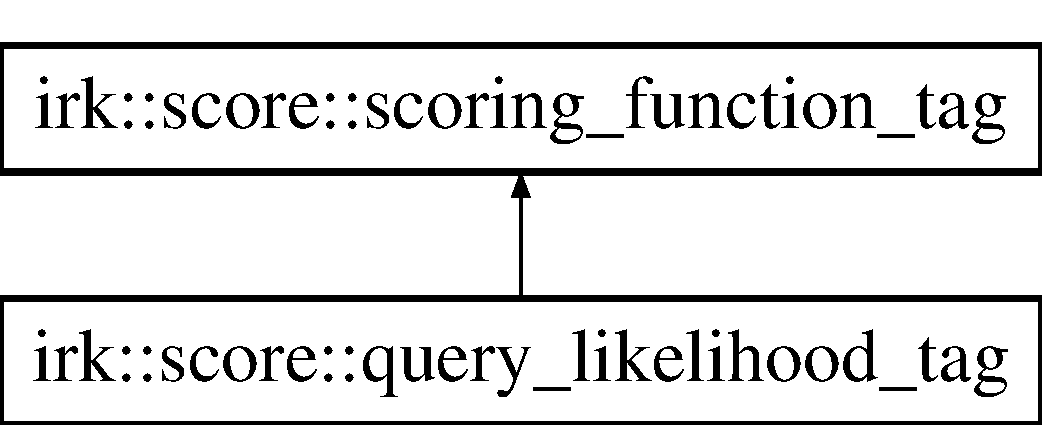
\includegraphics[height=2.000000cm]{structirk_1_1score_1_1query__likelihood__tag}
\end{center}
\end{figure}
\subsection*{Public Member Functions}
\begin{DoxyCompactItemize}
\item 
\mbox{\hyperlink{structirk_1_1score_1_1query__likelihood__tag_af0559f12be12863cf0fe6a6df56829f8}{operator std\+::string}} () override
\end{DoxyCompactItemize}


\subsection{Member Function Documentation}
\mbox{\Hypertarget{structirk_1_1score_1_1query__likelihood__tag_af0559f12be12863cf0fe6a6df56829f8}\label{structirk_1_1score_1_1query__likelihood__tag_af0559f12be12863cf0fe6a6df56829f8}} 
\index{irk\+::score\+::query\+\_\+likelihood\+\_\+tag@{irk\+::score\+::query\+\_\+likelihood\+\_\+tag}!operator std\+::string@{operator std\+::string}}
\index{operator std\+::string@{operator std\+::string}!irk\+::score\+::query\+\_\+likelihood\+\_\+tag@{irk\+::score\+::query\+\_\+likelihood\+\_\+tag}}
\subsubsection{\texorpdfstring{operator std\+::string()}{operator std::string()}}
{\footnotesize\ttfamily irk\+::score\+::query\+\_\+likelihood\+\_\+tag\+::operator std\+::string (\begin{DoxyParamCaption}{ }\end{DoxyParamCaption})\hspace{0.3cm}{\ttfamily [inline]}, {\ttfamily [override]}, {\ttfamily [virtual]}}



Implements \mbox{\hyperlink{structirk_1_1score_1_1scoring__function__tag_a718047dd6d5a9edd7b76ec55f2599c49}{irk\+::score\+::scoring\+\_\+function\+\_\+tag}}.



The documentation for this struct was generated from the following file\+:\begin{DoxyCompactItemize}
\item 
include/irkit/\mbox{\hyperlink{score_8hpp}{score.\+hpp}}\end{DoxyCompactItemize}

\hypertarget{classirk_1_1radix__tree}{}\section{irk\+:\+:radix\+\_\+tree$<$ T $>$ Class Template Reference}
\label{classirk_1_1radix__tree}\index{irk\+::radix\+\_\+tree$<$ T $>$@{irk\+::radix\+\_\+tree$<$ T $>$}}


{\ttfamily \#include $<$radix\+\_\+tree.\+hpp$>$}

\subsection*{Public Member Functions}
\begin{DoxyCompactItemize}
\item 
\mbox{\hyperlink{classirk_1_1radix__tree_a276f716ad240e75b4a3b2d1ee7c06663}{radix\+\_\+tree}} ()
\item 
\mbox{\hyperlink{classirk_1_1radix__tree_aaffbfdc0d841373868a7ca6672d0999f}{radix\+\_\+tree}} (const \mbox{\hyperlink{classirk_1_1radix__tree}{radix\+\_\+tree}} \&)=delete
\item 
\mbox{\hyperlink{classirk_1_1radix__tree_a83abd054182dee10a2a0f36c3974d420}{radix\+\_\+tree}} (\mbox{\hyperlink{classirk_1_1radix__tree}{radix\+\_\+tree}} \&\&other)=delete
\item 
\mbox{\hyperlink{classirk_1_1radix__tree}{radix\+\_\+tree}} \& \mbox{\hyperlink{classirk_1_1radix__tree_af052f00aa9f6f7ec58648365e28e30c8}{operator=}} (const \mbox{\hyperlink{classirk_1_1radix__tree}{radix\+\_\+tree}} \&)=delete
\item 
\mbox{\hyperlink{classirk_1_1radix__tree}{radix\+\_\+tree}} \& \mbox{\hyperlink{classirk_1_1radix__tree_a1b4f69f1e02478fe7b8a7dd590fef350}{operator=}} (\mbox{\hyperlink{classirk_1_1radix__tree}{radix\+\_\+tree}} \&\&)=delete
\item 
\mbox{\hyperlink{classirk_1_1radix__tree_a32491327f9b61b14c88f38ef6fd09a9f}{$\sim$radix\+\_\+tree}} ()
\item 
int \mbox{\hyperlink{classirk_1_1radix__tree_ad65f1ba2c32c59c3b6fd2ca220a9fc7f}{insert}} (const std\+::string \&key, T value)
\item 
{\footnotesize template$<$class  = enable\+\_\+if\+\_\+not\+\_\+equal$<$\+T, void$>$$>$ }\\T \mbox{\hyperlink{classirk_1_1radix__tree_af46c8d034084c54b33bb761ec96588d4}{operator\mbox{[}$\,$\mbox{]}}} (const std\+::string \&key)
\item 
{\footnotesize template$<$class  = enable\+\_\+if\+\_\+not\+\_\+equal$<$\+T, void$>$$>$ }\\std\+::optional$<$ T $>$ \mbox{\hyperlink{classirk_1_1radix__tree_a7a8f4484dd52244e712e204288e00b15}{find}} (const std\+::string \&key)
\item 
bool \mbox{\hyperlink{classirk_1_1radix__tree_a3b9cecf1586c0e96b3ea55224db7c389}{exists}} (const std\+::string \&key)
\item 
std\+::optional$<$ T $>$ \mbox{\hyperlink{classirk_1_1radix__tree_aec3e27fbf3cd3f0e2d75183d392b0946}{seek\+\_\+le}} (std\+::string key) const
\item 
rax $\ast$ \mbox{\hyperlink{classirk_1_1radix__tree_aed4255775e1f9f2a4647e80a408c9946}{c\+\_\+rax}} () const
\end{DoxyCompactItemize}


\subsection{Constructor \& Destructor Documentation}
\mbox{\Hypertarget{classirk_1_1radix__tree_a276f716ad240e75b4a3b2d1ee7c06663}\label{classirk_1_1radix__tree_a276f716ad240e75b4a3b2d1ee7c06663}} 
\index{irk\+::radix\+\_\+tree@{irk\+::radix\+\_\+tree}!radix\+\_\+tree@{radix\+\_\+tree}}
\index{radix\+\_\+tree@{radix\+\_\+tree}!irk\+::radix\+\_\+tree@{irk\+::radix\+\_\+tree}}
\subsubsection{\texorpdfstring{radix\+\_\+tree()}{radix\_tree()}\hspace{0.1cm}{\footnotesize\ttfamily [1/3]}}
{\footnotesize\ttfamily template$<$class T $>$ \\
\mbox{\hyperlink{classirk_1_1radix__tree}{irk\+::radix\+\_\+tree}}$<$ T $>$\+::\mbox{\hyperlink{classirk_1_1radix__tree}{radix\+\_\+tree}} (\begin{DoxyParamCaption}{ }\end{DoxyParamCaption})\hspace{0.3cm}{\ttfamily [inline]}}

\mbox{\Hypertarget{classirk_1_1radix__tree_aaffbfdc0d841373868a7ca6672d0999f}\label{classirk_1_1radix__tree_aaffbfdc0d841373868a7ca6672d0999f}} 
\index{irk\+::radix\+\_\+tree@{irk\+::radix\+\_\+tree}!radix\+\_\+tree@{radix\+\_\+tree}}
\index{radix\+\_\+tree@{radix\+\_\+tree}!irk\+::radix\+\_\+tree@{irk\+::radix\+\_\+tree}}
\subsubsection{\texorpdfstring{radix\+\_\+tree()}{radix\_tree()}\hspace{0.1cm}{\footnotesize\ttfamily [2/3]}}
{\footnotesize\ttfamily template$<$class T $>$ \\
\mbox{\hyperlink{classirk_1_1radix__tree}{irk\+::radix\+\_\+tree}}$<$ T $>$\+::\mbox{\hyperlink{classirk_1_1radix__tree}{radix\+\_\+tree}} (\begin{DoxyParamCaption}\item[{const \mbox{\hyperlink{classirk_1_1radix__tree}{radix\+\_\+tree}}$<$ T $>$ \&}]{ }\end{DoxyParamCaption})\hspace{0.3cm}{\ttfamily [delete]}}

\mbox{\Hypertarget{classirk_1_1radix__tree_a83abd054182dee10a2a0f36c3974d420}\label{classirk_1_1radix__tree_a83abd054182dee10a2a0f36c3974d420}} 
\index{irk\+::radix\+\_\+tree@{irk\+::radix\+\_\+tree}!radix\+\_\+tree@{radix\+\_\+tree}}
\index{radix\+\_\+tree@{radix\+\_\+tree}!irk\+::radix\+\_\+tree@{irk\+::radix\+\_\+tree}}
\subsubsection{\texorpdfstring{radix\+\_\+tree()}{radix\_tree()}\hspace{0.1cm}{\footnotesize\ttfamily [3/3]}}
{\footnotesize\ttfamily template$<$class T $>$ \\
\mbox{\hyperlink{classirk_1_1radix__tree}{irk\+::radix\+\_\+tree}}$<$ T $>$\+::\mbox{\hyperlink{classirk_1_1radix__tree}{radix\+\_\+tree}} (\begin{DoxyParamCaption}\item[{\mbox{\hyperlink{classirk_1_1radix__tree}{radix\+\_\+tree}}$<$ T $>$ \&\&}]{other }\end{DoxyParamCaption})\hspace{0.3cm}{\ttfamily [delete]}}

\mbox{\Hypertarget{classirk_1_1radix__tree_a32491327f9b61b14c88f38ef6fd09a9f}\label{classirk_1_1radix__tree_a32491327f9b61b14c88f38ef6fd09a9f}} 
\index{irk\+::radix\+\_\+tree@{irk\+::radix\+\_\+tree}!````~radix\+\_\+tree@{$\sim$radix\+\_\+tree}}
\index{````~radix\+\_\+tree@{$\sim$radix\+\_\+tree}!irk\+::radix\+\_\+tree@{irk\+::radix\+\_\+tree}}
\subsubsection{\texorpdfstring{$\sim$radix\+\_\+tree()}{~radix\_tree()}}
{\footnotesize\ttfamily template$<$class T $>$ \\
\mbox{\hyperlink{classirk_1_1radix__tree}{irk\+::radix\+\_\+tree}}$<$ T $>$\+::$\sim$\mbox{\hyperlink{classirk_1_1radix__tree}{radix\+\_\+tree}} (\begin{DoxyParamCaption}{ }\end{DoxyParamCaption})\hspace{0.3cm}{\ttfamily [inline]}}



\subsection{Member Function Documentation}
\mbox{\Hypertarget{classirk_1_1radix__tree_aed4255775e1f9f2a4647e80a408c9946}\label{classirk_1_1radix__tree_aed4255775e1f9f2a4647e80a408c9946}} 
\index{irk\+::radix\+\_\+tree@{irk\+::radix\+\_\+tree}!c\+\_\+rax@{c\+\_\+rax}}
\index{c\+\_\+rax@{c\+\_\+rax}!irk\+::radix\+\_\+tree@{irk\+::radix\+\_\+tree}}
\subsubsection{\texorpdfstring{c\+\_\+rax()}{c\_rax()}}
{\footnotesize\ttfamily template$<$class T $>$ \\
rax$\ast$ \mbox{\hyperlink{classirk_1_1radix__tree}{irk\+::radix\+\_\+tree}}$<$ T $>$\+::c\+\_\+rax (\begin{DoxyParamCaption}{ }\end{DoxyParamCaption}) const\hspace{0.3cm}{\ttfamily [inline]}}

\mbox{\Hypertarget{classirk_1_1radix__tree_a3b9cecf1586c0e96b3ea55224db7c389}\label{classirk_1_1radix__tree_a3b9cecf1586c0e96b3ea55224db7c389}} 
\index{irk\+::radix\+\_\+tree@{irk\+::radix\+\_\+tree}!exists@{exists}}
\index{exists@{exists}!irk\+::radix\+\_\+tree@{irk\+::radix\+\_\+tree}}
\subsubsection{\texorpdfstring{exists()}{exists()}}
{\footnotesize\ttfamily template$<$class T $>$ \\
bool \mbox{\hyperlink{classirk_1_1radix__tree}{irk\+::radix\+\_\+tree}}$<$ T $>$\+::exists (\begin{DoxyParamCaption}\item[{const std\+::string \&}]{key }\end{DoxyParamCaption})\hspace{0.3cm}{\ttfamily [inline]}}

\mbox{\Hypertarget{classirk_1_1radix__tree_a7a8f4484dd52244e712e204288e00b15}\label{classirk_1_1radix__tree_a7a8f4484dd52244e712e204288e00b15}} 
\index{irk\+::radix\+\_\+tree@{irk\+::radix\+\_\+tree}!find@{find}}
\index{find@{find}!irk\+::radix\+\_\+tree@{irk\+::radix\+\_\+tree}}
\subsubsection{\texorpdfstring{find()}{find()}}
{\footnotesize\ttfamily template$<$class T $>$ \\
template$<$class  = enable\+\_\+if\+\_\+not\+\_\+equal$<$\+T, void$>$$>$ \\
std\+::optional$<$T$>$ \mbox{\hyperlink{classirk_1_1radix__tree}{irk\+::radix\+\_\+tree}}$<$ T $>$\+::find (\begin{DoxyParamCaption}\item[{const std\+::string \&}]{key }\end{DoxyParamCaption})\hspace{0.3cm}{\ttfamily [inline]}}

\mbox{\Hypertarget{classirk_1_1radix__tree_ad65f1ba2c32c59c3b6fd2ca220a9fc7f}\label{classirk_1_1radix__tree_ad65f1ba2c32c59c3b6fd2ca220a9fc7f}} 
\index{irk\+::radix\+\_\+tree@{irk\+::radix\+\_\+tree}!insert@{insert}}
\index{insert@{insert}!irk\+::radix\+\_\+tree@{irk\+::radix\+\_\+tree}}
\subsubsection{\texorpdfstring{insert()}{insert()}}
{\footnotesize\ttfamily template$<$class T $>$ \\
int \mbox{\hyperlink{classirk_1_1radix__tree}{irk\+::radix\+\_\+tree}}$<$ T $>$\+::insert (\begin{DoxyParamCaption}\item[{const std\+::string \&}]{key,  }\item[{T}]{value }\end{DoxyParamCaption})\hspace{0.3cm}{\ttfamily [inline]}}

\mbox{\Hypertarget{classirk_1_1radix__tree_af052f00aa9f6f7ec58648365e28e30c8}\label{classirk_1_1radix__tree_af052f00aa9f6f7ec58648365e28e30c8}} 
\index{irk\+::radix\+\_\+tree@{irk\+::radix\+\_\+tree}!operator=@{operator=}}
\index{operator=@{operator=}!irk\+::radix\+\_\+tree@{irk\+::radix\+\_\+tree}}
\subsubsection{\texorpdfstring{operator=()}{operator=()}\hspace{0.1cm}{\footnotesize\ttfamily [1/2]}}
{\footnotesize\ttfamily template$<$class T $>$ \\
\mbox{\hyperlink{classirk_1_1radix__tree}{radix\+\_\+tree}}\& \mbox{\hyperlink{classirk_1_1radix__tree}{irk\+::radix\+\_\+tree}}$<$ T $>$\+::operator= (\begin{DoxyParamCaption}\item[{const \mbox{\hyperlink{classirk_1_1radix__tree}{radix\+\_\+tree}}$<$ T $>$ \&}]{ }\end{DoxyParamCaption})\hspace{0.3cm}{\ttfamily [delete]}}

\mbox{\Hypertarget{classirk_1_1radix__tree_a1b4f69f1e02478fe7b8a7dd590fef350}\label{classirk_1_1radix__tree_a1b4f69f1e02478fe7b8a7dd590fef350}} 
\index{irk\+::radix\+\_\+tree@{irk\+::radix\+\_\+tree}!operator=@{operator=}}
\index{operator=@{operator=}!irk\+::radix\+\_\+tree@{irk\+::radix\+\_\+tree}}
\subsubsection{\texorpdfstring{operator=()}{operator=()}\hspace{0.1cm}{\footnotesize\ttfamily [2/2]}}
{\footnotesize\ttfamily template$<$class T $>$ \\
\mbox{\hyperlink{classirk_1_1radix__tree}{radix\+\_\+tree}}\& \mbox{\hyperlink{classirk_1_1radix__tree}{irk\+::radix\+\_\+tree}}$<$ T $>$\+::operator= (\begin{DoxyParamCaption}\item[{\mbox{\hyperlink{classirk_1_1radix__tree}{radix\+\_\+tree}}$<$ T $>$ \&\&}]{ }\end{DoxyParamCaption})\hspace{0.3cm}{\ttfamily [delete]}}

\mbox{\Hypertarget{classirk_1_1radix__tree_af46c8d034084c54b33bb761ec96588d4}\label{classirk_1_1radix__tree_af46c8d034084c54b33bb761ec96588d4}} 
\index{irk\+::radix\+\_\+tree@{irk\+::radix\+\_\+tree}!operator\mbox{[}\mbox{]}@{operator[]}}
\index{operator\mbox{[}\mbox{]}@{operator[]}!irk\+::radix\+\_\+tree@{irk\+::radix\+\_\+tree}}
\subsubsection{\texorpdfstring{operator[]()}{operator[]()}}
{\footnotesize\ttfamily template$<$class T $>$ \\
template$<$class  = enable\+\_\+if\+\_\+not\+\_\+equal$<$\+T, void$>$$>$ \\
T \mbox{\hyperlink{classirk_1_1radix__tree}{irk\+::radix\+\_\+tree}}$<$ T $>$\+::operator\mbox{[}$\,$\mbox{]} (\begin{DoxyParamCaption}\item[{const std\+::string \&}]{key }\end{DoxyParamCaption})\hspace{0.3cm}{\ttfamily [inline]}}

\mbox{\Hypertarget{classirk_1_1radix__tree_aec3e27fbf3cd3f0e2d75183d392b0946}\label{classirk_1_1radix__tree_aec3e27fbf3cd3f0e2d75183d392b0946}} 
\index{irk\+::radix\+\_\+tree@{irk\+::radix\+\_\+tree}!seek\+\_\+le@{seek\+\_\+le}}
\index{seek\+\_\+le@{seek\+\_\+le}!irk\+::radix\+\_\+tree@{irk\+::radix\+\_\+tree}}
\subsubsection{\texorpdfstring{seek\+\_\+le()}{seek\_le()}}
{\footnotesize\ttfamily template$<$class T $>$ \\
std\+::optional$<$T$>$ \mbox{\hyperlink{classirk_1_1radix__tree}{irk\+::radix\+\_\+tree}}$<$ T $>$\+::seek\+\_\+le (\begin{DoxyParamCaption}\item[{std\+::string}]{key }\end{DoxyParamCaption}) const\hspace{0.3cm}{\ttfamily [inline]}}



The documentation for this class was generated from the following file\+:\begin{DoxyCompactItemize}
\item 
include/irkit/\mbox{\hyperlink{radix__tree_8hpp}{radix\+\_\+tree.\+hpp}}\end{DoxyCompactItemize}

\hypertarget{structirk_1_1bitptr_1_1reader}{}\section{irk\+:\+:bitptr$<$ Block $>$\+:\+:reader Struct Reference}
\label{structirk_1_1bitptr_1_1reader}\index{irk\+::bitptr$<$ Block $>$\+::reader@{irk\+::bitptr$<$ Block $>$\+::reader}}


{\ttfamily \#include $<$bitptr.\+hpp$>$}

\subsection*{Public Member Functions}
\begin{DoxyCompactItemize}
\item 
bool \mbox{\hyperlink{structirk_1_1bitptr_1_1reader_ae3eaee83cecc7193fc16a1f31cdddb92}{read}} ()
\end{DoxyCompactItemize}
\subsection*{Public Attributes}
\begin{DoxyCompactItemize}
\item 
\mbox{\hyperlink{classirk_1_1bitptr}{bitptr}} \& \mbox{\hyperlink{structirk_1_1bitptr_1_1reader_af27825b949fe047a40e95730fd7631d3}{pos}}
\end{DoxyCompactItemize}


\subsection{Detailed Description}
\subsubsection*{template$<$class Block$>$\newline
struct irk\+::bitptr$<$ Block $>$\+::reader}

A type that can be used as a bit input stream that automatically moves its pointer. ~\newline


{\bfseries Warning}\+: The type is incomplete! So far it only implements {\ttfamily \mbox{\hyperlink{structirk_1_1bitptr_1_1reader_ae3eaee83cecc7193fc16a1f31cdddb92}{read()}}} function. 

\subsection{Member Function Documentation}
\mbox{\Hypertarget{structirk_1_1bitptr_1_1reader_ae3eaee83cecc7193fc16a1f31cdddb92}\label{structirk_1_1bitptr_1_1reader_ae3eaee83cecc7193fc16a1f31cdddb92}} 
\index{irk\+::bitptr\+::reader@{irk\+::bitptr\+::reader}!read@{read}}
\index{read@{read}!irk\+::bitptr\+::reader@{irk\+::bitptr\+::reader}}
\subsubsection{\texorpdfstring{read()}{read()}}
{\footnotesize\ttfamily template$<$class Block$>$ \\
bool \mbox{\hyperlink{classirk_1_1bitptr}{irk\+::bitptr}}$<$ Block $>$\+::reader\+::read (\begin{DoxyParamCaption}{ }\end{DoxyParamCaption})\hspace{0.3cm}{\ttfamily [inline]}}



\subsection{Member Data Documentation}
\mbox{\Hypertarget{structirk_1_1bitptr_1_1reader_af27825b949fe047a40e95730fd7631d3}\label{structirk_1_1bitptr_1_1reader_af27825b949fe047a40e95730fd7631d3}} 
\index{irk\+::bitptr\+::reader@{irk\+::bitptr\+::reader}!pos@{pos}}
\index{pos@{pos}!irk\+::bitptr\+::reader@{irk\+::bitptr\+::reader}}
\subsubsection{\texorpdfstring{pos}{pos}}
{\footnotesize\ttfamily template$<$class Block$>$ \\
\mbox{\hyperlink{classirk_1_1bitptr}{bitptr}}\& \mbox{\hyperlink{classirk_1_1bitptr}{irk\+::bitptr}}$<$ Block $>$\+::reader\+::pos}



The documentation for this struct was generated from the following file\+:\begin{DoxyCompactItemize}
\item 
include/irkit/\mbox{\hyperlink{bitptr_8hpp}{bitptr.\+hpp}}\end{DoxyCompactItemize}

\hypertarget{structirk_1_1reinterpret__cast__fn}{}\section{irk\+:\+:reinterpret\+\_\+cast\+\_\+fn$<$ T $>$ Struct Template Reference}
\label{structirk_1_1reinterpret__cast__fn}\index{irk\+::reinterpret\+\_\+cast\+\_\+fn$<$ T $>$@{irk\+::reinterpret\+\_\+cast\+\_\+fn$<$ T $>$}}


{\ttfamily \#include $<$memoryview.\+hpp$>$}

\subsection*{Public Member Functions}
\begin{DoxyCompactItemize}
\item 
T \mbox{\hyperlink{structirk_1_1reinterpret__cast__fn_a52b9dc0045937a8e52cfc66ee834d54c}{operator()}} (const char $\ast$pos) const
\end{DoxyCompactItemize}


\subsection{Member Function Documentation}
\mbox{\Hypertarget{structirk_1_1reinterpret__cast__fn_a52b9dc0045937a8e52cfc66ee834d54c}\label{structirk_1_1reinterpret__cast__fn_a52b9dc0045937a8e52cfc66ee834d54c}} 
\index{irk\+::reinterpret\+\_\+cast\+\_\+fn@{irk\+::reinterpret\+\_\+cast\+\_\+fn}!operator()@{operator()}}
\index{operator()@{operator()}!irk\+::reinterpret\+\_\+cast\+\_\+fn@{irk\+::reinterpret\+\_\+cast\+\_\+fn}}
\subsubsection{\texorpdfstring{operator()()}{operator()()}}
{\footnotesize\ttfamily template$<$class T $>$ \\
T \mbox{\hyperlink{structirk_1_1reinterpret__cast__fn}{irk\+::reinterpret\+\_\+cast\+\_\+fn}}$<$ T $>$\+::operator() (\begin{DoxyParamCaption}\item[{const char $\ast$}]{pos }\end{DoxyParamCaption}) const\hspace{0.3cm}{\ttfamily [inline]}}



The documentation for this struct was generated from the following file\+:\begin{DoxyCompactItemize}
\item 
include/irkit/\mbox{\hyperlink{memoryview_8hpp}{memoryview.\+hpp}}\end{DoxyCompactItemize}

\hypertarget{structirk_1_1score_1_1scoring__function__tag}{}\section{irk\+:\+:score\+:\+:scoring\+\_\+function\+\_\+tag Struct Reference}
\label{structirk_1_1score_1_1scoring__function__tag}\index{irk\+::score\+::scoring\+\_\+function\+\_\+tag@{irk\+::score\+::scoring\+\_\+function\+\_\+tag}}


{\ttfamily \#include $<$score.\+hpp$>$}

Inheritance diagram for irk\+:\+:score\+:\+:scoring\+\_\+function\+\_\+tag\+:\begin{figure}[H]
\begin{center}
\leavevmode
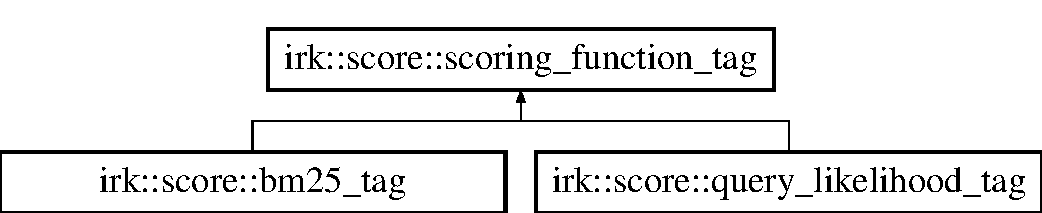
\includegraphics[height=2.000000cm]{structirk_1_1score_1_1scoring__function__tag}
\end{center}
\end{figure}
\subsection*{Public Member Functions}
\begin{DoxyCompactItemize}
\item 
virtual \mbox{\hyperlink{structirk_1_1score_1_1scoring__function__tag_a718047dd6d5a9edd7b76ec55f2599c49}{operator std\+::string}} ()=0
\end{DoxyCompactItemize}


\subsection{Member Function Documentation}
\mbox{\Hypertarget{structirk_1_1score_1_1scoring__function__tag_a718047dd6d5a9edd7b76ec55f2599c49}\label{structirk_1_1score_1_1scoring__function__tag_a718047dd6d5a9edd7b76ec55f2599c49}} 
\index{irk\+::score\+::scoring\+\_\+function\+\_\+tag@{irk\+::score\+::scoring\+\_\+function\+\_\+tag}!operator std\+::string@{operator std\+::string}}
\index{operator std\+::string@{operator std\+::string}!irk\+::score\+::scoring\+\_\+function\+\_\+tag@{irk\+::score\+::scoring\+\_\+function\+\_\+tag}}
\subsubsection{\texorpdfstring{operator std\+::string()}{operator std::string()}}
{\footnotesize\ttfamily virtual irk\+::score\+::scoring\+\_\+function\+\_\+tag\+::operator std\+::string (\begin{DoxyParamCaption}{ }\end{DoxyParamCaption})\hspace{0.3cm}{\ttfamily [explicit]}, {\ttfamily [pure virtual]}}



Implemented in \mbox{\hyperlink{structirk_1_1score_1_1query__likelihood__tag_af0559f12be12863cf0fe6a6df56829f8}{irk\+::score\+::query\+\_\+likelihood\+\_\+tag}}, and \mbox{\hyperlink{structirk_1_1score_1_1bm25__tag_a3575a5c838ad5a235198d525e665e0f1}{irk\+::score\+::bm25\+\_\+tag}}.



The documentation for this struct was generated from the following file\+:\begin{DoxyCompactItemize}
\item 
include/irkit/\mbox{\hyperlink{score_8hpp}{score.\+hpp}}\end{DoxyCompactItemize}

\hypertarget{classirk_1_1simple__accumulator}{}\section{irk\+:\+:simple\+\_\+accumulator Class Reference}
\label{classirk_1_1simple__accumulator}\index{irk\+::simple\+\_\+accumulator@{irk\+::simple\+\_\+accumulator}}


A simple score accumulator that adds all scores.  




{\ttfamily \#include $<$taat.\+hpp$>$}

\subsection*{Public Member Functions}
\begin{DoxyCompactItemize}
\item 
{\footnotesize template$<$class Doc , class Score , class Accumulator\+Array $>$ }\\void \mbox{\hyperlink{classirk_1_1simple__accumulator_a641d831933fba432b05f485829e3b8d4}{accumulate\+\_\+posting}} (Doc doc, Score score\+\_\+delta, Accumulator\+Array \&acc)
\end{DoxyCompactItemize}


\subsection{Detailed Description}
A simple score accumulator that adds all scores. 

\subsection{Member Function Documentation}
\mbox{\Hypertarget{classirk_1_1simple__accumulator_a641d831933fba432b05f485829e3b8d4}\label{classirk_1_1simple__accumulator_a641d831933fba432b05f485829e3b8d4}} 
\index{irk\+::simple\+\_\+accumulator@{irk\+::simple\+\_\+accumulator}!accumulate\+\_\+posting@{accumulate\+\_\+posting}}
\index{accumulate\+\_\+posting@{accumulate\+\_\+posting}!irk\+::simple\+\_\+accumulator@{irk\+::simple\+\_\+accumulator}}
\subsubsection{\texorpdfstring{accumulate\+\_\+posting()}{accumulate\_posting()}}
{\footnotesize\ttfamily template$<$class Doc , class Score , class Accumulator\+Array $>$ \\
void irk\+::simple\+\_\+accumulator\+::accumulate\+\_\+posting (\begin{DoxyParamCaption}\item[{Doc}]{doc,  }\item[{Score}]{score\+\_\+delta,  }\item[{Accumulator\+Array \&}]{acc }\end{DoxyParamCaption})\hspace{0.3cm}{\ttfamily [inline]}}



The documentation for this class was generated from the following file\+:\begin{DoxyCompactItemize}
\item 
include/irkit/\mbox{\hyperlink{taat_8hpp}{taat.\+hpp}}\end{DoxyCompactItemize}

\hypertarget{classirk_1_1index_1_1skip__list__builder}{}\section{irk\+:\+:index\+:\+:skip\+\_\+list\+\_\+builder$<$ Skip, element\+\_\+size, Write\+Fn $>$ Class Template Reference}
\label{classirk_1_1index_1_1skip__list__builder}\index{irk\+::index\+::skip\+\_\+list\+\_\+builder$<$ Skip, element\+\_\+size, Write\+Fn $>$@{irk\+::index\+::skip\+\_\+list\+\_\+builder$<$ Skip, element\+\_\+size, Write\+Fn $>$}}


Builds and writes skip lists for postings.  




{\ttfamily \#include $<$skiplist.\+hpp$>$}

\subsection*{Public Member Functions}
\begin{DoxyCompactItemize}
\item 
\mbox{\hyperlink{classirk_1_1index_1_1skip__list__builder_a55f45083c19eb7e4a03aeda3e5e1c501}{skip\+\_\+list\+\_\+builder}} (std\+::ostream \&skips\+\_\+out, std\+::ostream \&offsets\+\_\+out, int block\+\_\+size) noexcept
\item 
void \mbox{\hyperlink{classirk_1_1index_1_1skip__list__builder_ae3526c260650dda4bd771087927fe871}{write\+\_\+term\+\_\+skips}} ()
\item 
void \mbox{\hyperlink{classirk_1_1index_1_1skip__list__builder_afddff8af3fc2fdd09950ae6036b2bc0c}{close}} () const
\end{DoxyCompactItemize}


\subsection{Detailed Description}
\subsubsection*{template$<$class Skip, int element\+\_\+size = sizeof(\+Skip), class Write\+Fn = write\+\_\+fn$<$\+Skip$>$$>$\newline
class irk\+::index\+::skip\+\_\+list\+\_\+builder$<$ Skip, element\+\_\+size, Write\+Fn $>$}

Builds and writes skip lists for postings. 

\subsection{Constructor \& Destructor Documentation}
\mbox{\Hypertarget{classirk_1_1index_1_1skip__list__builder_a55f45083c19eb7e4a03aeda3e5e1c501}\label{classirk_1_1index_1_1skip__list__builder_a55f45083c19eb7e4a03aeda3e5e1c501}} 
\index{irk\+::index\+::skip\+\_\+list\+\_\+builder@{irk\+::index\+::skip\+\_\+list\+\_\+builder}!skip\+\_\+list\+\_\+builder@{skip\+\_\+list\+\_\+builder}}
\index{skip\+\_\+list\+\_\+builder@{skip\+\_\+list\+\_\+builder}!irk\+::index\+::skip\+\_\+list\+\_\+builder@{irk\+::index\+::skip\+\_\+list\+\_\+builder}}
\subsubsection{\texorpdfstring{skip\+\_\+list\+\_\+builder()}{skip\_list\_builder()}}
{\footnotesize\ttfamily template$<$class Skip , int element\+\_\+size = sizeof(\+Skip), class Write\+Fn  = write\+\_\+fn$<$\+Skip$>$$>$ \\
\mbox{\hyperlink{classirk_1_1index_1_1skip__list__builder}{irk\+::index\+::skip\+\_\+list\+\_\+builder}}$<$ Skip, element\+\_\+size, Write\+Fn $>$\+::\mbox{\hyperlink{classirk_1_1index_1_1skip__list__builder}{skip\+\_\+list\+\_\+builder}} (\begin{DoxyParamCaption}\item[{std\+::ostream \&}]{skips\+\_\+out,  }\item[{std\+::ostream \&}]{offsets\+\_\+out,  }\item[{int}]{block\+\_\+size }\end{DoxyParamCaption})\hspace{0.3cm}{\ttfamily [inline]}, {\ttfamily [noexcept]}}



\subsection{Member Function Documentation}
\mbox{\Hypertarget{classirk_1_1index_1_1skip__list__builder_afddff8af3fc2fdd09950ae6036b2bc0c}\label{classirk_1_1index_1_1skip__list__builder_afddff8af3fc2fdd09950ae6036b2bc0c}} 
\index{irk\+::index\+::skip\+\_\+list\+\_\+builder@{irk\+::index\+::skip\+\_\+list\+\_\+builder}!close@{close}}
\index{close@{close}!irk\+::index\+::skip\+\_\+list\+\_\+builder@{irk\+::index\+::skip\+\_\+list\+\_\+builder}}
\subsubsection{\texorpdfstring{close()}{close()}}
{\footnotesize\ttfamily template$<$class Skip , int element\+\_\+size = sizeof(\+Skip), class Write\+Fn  = write\+\_\+fn$<$\+Skip$>$$>$ \\
void \mbox{\hyperlink{classirk_1_1index_1_1skip__list__builder}{irk\+::index\+::skip\+\_\+list\+\_\+builder}}$<$ Skip, element\+\_\+size, Write\+Fn $>$\+::close (\begin{DoxyParamCaption}{ }\end{DoxyParamCaption}) const\hspace{0.3cm}{\ttfamily [inline]}}

\mbox{\Hypertarget{classirk_1_1index_1_1skip__list__builder_ae3526c260650dda4bd771087927fe871}\label{classirk_1_1index_1_1skip__list__builder_ae3526c260650dda4bd771087927fe871}} 
\index{irk\+::index\+::skip\+\_\+list\+\_\+builder@{irk\+::index\+::skip\+\_\+list\+\_\+builder}!write\+\_\+term\+\_\+skips@{write\+\_\+term\+\_\+skips}}
\index{write\+\_\+term\+\_\+skips@{write\+\_\+term\+\_\+skips}!irk\+::index\+::skip\+\_\+list\+\_\+builder@{irk\+::index\+::skip\+\_\+list\+\_\+builder}}
\subsubsection{\texorpdfstring{write\+\_\+term\+\_\+skips()}{write\_term\_skips()}}
{\footnotesize\ttfamily template$<$class Skip , int element\+\_\+size = sizeof(\+Skip), class Write\+Fn  = write\+\_\+fn$<$\+Skip$>$$>$ \\
void \mbox{\hyperlink{classirk_1_1index_1_1skip__list__builder}{irk\+::index\+::skip\+\_\+list\+\_\+builder}}$<$ Skip, element\+\_\+size, Write\+Fn $>$\+::write\+\_\+term\+\_\+skips (\begin{DoxyParamCaption}{ }\end{DoxyParamCaption})\hspace{0.3cm}{\ttfamily [inline]}}



The documentation for this class was generated from the following file\+:\begin{DoxyCompactItemize}
\item 
include/irkit/index/\mbox{\hyperlink{skiplist_8hpp}{skiplist.\+hpp}}\end{DoxyCompactItemize}

\hypertarget{classirk_1_1index_1_1skip__list__view}{}\section{irk\+:\+:index\+:\+:skip\+\_\+list\+\_\+view$<$ Skip, element\+\_\+size, Cast\+Fn $>$ Class Template Reference}
\label{classirk_1_1index_1_1skip__list__view}\index{irk\+::index\+::skip\+\_\+list\+\_\+view$<$ Skip, element\+\_\+size, Cast\+Fn $>$@{irk\+::index\+::skip\+\_\+list\+\_\+view$<$ Skip, element\+\_\+size, Cast\+Fn $>$}}


{\ttfamily \#include $<$skiplist.\+hpp$>$}

\subsection*{Classes}
\begin{DoxyCompactItemize}
\item 
struct \mbox{\hyperlink{structirk_1_1index_1_1skip__list__view_1_1const__iterator}{const\+\_\+iterator}}
\end{DoxyCompactItemize}
\subsection*{Public Types}
\begin{DoxyCompactItemize}
\item 
using \mbox{\hyperlink{classirk_1_1index_1_1skip__list__view_a7fa2224428803eee24062bb123978755}{skip\+\_\+type}} = Skip
\item 
using \mbox{\hyperlink{classirk_1_1index_1_1skip__list__view_a7e7a81a64ede6bcd7c49bc05cd6243d3}{iterator}} = \mbox{\hyperlink{structirk_1_1index_1_1skip__list__view_1_1const__iterator}{const\+\_\+iterator}}
\end{DoxyCompactItemize}
\subsection*{Public Member Functions}
\begin{DoxyCompactItemize}
\item 
\mbox{\hyperlink{classirk_1_1index_1_1skip__list__view_a97abe4d23715e60ef30892bdd8ad9cd7}{skip\+\_\+list\+\_\+view}} ()=default
\item 
\mbox{\hyperlink{classirk_1_1index_1_1skip__list__view_ab77d6c40db66d837d83675767b25f6f8}{skip\+\_\+list\+\_\+view}} (const \mbox{\hyperlink{classirk_1_1index_1_1skip__list__view}{skip\+\_\+list\+\_\+view}} \&)=default
\item 
\mbox{\hyperlink{classirk_1_1index_1_1skip__list__view_a2e1d39b4efd56dd98ead2a39713d5508}{skip\+\_\+list\+\_\+view}} (\mbox{\hyperlink{classirk_1_1index_1_1skip__list__view}{skip\+\_\+list\+\_\+view}} \&\&)=default
\item 
\mbox{\hyperlink{classirk_1_1index_1_1skip__list__view_a9cadb9826ca85f857e83781ca811f6d3}{skip\+\_\+list\+\_\+view}} (\mbox{\hyperlink{classirk_1_1memory__view}{irk\+::memory\+\_\+view}} \mbox{\hyperlink{classirk_1_1memory__view}{memory\+\_\+view}})
\item 
auto \mbox{\hyperlink{classirk_1_1index_1_1skip__list__view_a923176e9b8851cea6f32f530ad88d25c}{block\+\_\+count}} () const noexcept
\item 
auto \mbox{\hyperlink{classirk_1_1index_1_1skip__list__view_ab77e0b9d495904034e1948609089cf28}{size}} () const noexcept
\item 
constexpr \mbox{\hyperlink{structirk_1_1index_1_1skip__list__view_1_1const__iterator}{const\+\_\+iterator}} \mbox{\hyperlink{classirk_1_1index_1_1skip__list__view_a22e0239c33e18137997aad3da5337591}{begin}} () const noexcept
\item 
constexpr \mbox{\hyperlink{structirk_1_1index_1_1skip__list__view_1_1const__iterator}{const\+\_\+iterator}} \mbox{\hyperlink{classirk_1_1index_1_1skip__list__view_ae6a3b8d467288b8dd044d0ff3fab48a5}{cbegin}} () const noexcept
\item 
constexpr \mbox{\hyperlink{structirk_1_1index_1_1skip__list__view_1_1const__iterator}{const\+\_\+iterator}} \mbox{\hyperlink{classirk_1_1index_1_1skip__list__view_aa22abee7366f281e77e8ab0f556832a5}{end}} () const noexcept
\item 
constexpr \mbox{\hyperlink{structirk_1_1index_1_1skip__list__view_1_1const__iterator}{const\+\_\+iterator}} \mbox{\hyperlink{classirk_1_1index_1_1skip__list__view_afce38149f8be877dd4426e16da060dc6}{cend}} () const noexcept
\end{DoxyCompactItemize}


\subsection{Member Typedef Documentation}
\mbox{\Hypertarget{classirk_1_1index_1_1skip__list__view_a7e7a81a64ede6bcd7c49bc05cd6243d3}\label{classirk_1_1index_1_1skip__list__view_a7e7a81a64ede6bcd7c49bc05cd6243d3}} 
\index{irk\+::index\+::skip\+\_\+list\+\_\+view@{irk\+::index\+::skip\+\_\+list\+\_\+view}!iterator@{iterator}}
\index{iterator@{iterator}!irk\+::index\+::skip\+\_\+list\+\_\+view@{irk\+::index\+::skip\+\_\+list\+\_\+view}}
\subsubsection{\texorpdfstring{iterator}{iterator}}
{\footnotesize\ttfamily template$<$class Skip , int element\+\_\+size = sizeof(\+Skip), class Cast\+Fn  = irk\+::reinterpret\+\_\+cast\+\_\+fn$<$\+Skip$>$$>$ \\
using \mbox{\hyperlink{classirk_1_1index_1_1skip__list__view}{irk\+::index\+::skip\+\_\+list\+\_\+view}}$<$ Skip, element\+\_\+size, Cast\+Fn $>$\+::\mbox{\hyperlink{classirk_1_1index_1_1skip__list__view_a7e7a81a64ede6bcd7c49bc05cd6243d3}{iterator}} =  \mbox{\hyperlink{structirk_1_1index_1_1skip__list__view_1_1const__iterator}{const\+\_\+iterator}}}

\mbox{\Hypertarget{classirk_1_1index_1_1skip__list__view_a7fa2224428803eee24062bb123978755}\label{classirk_1_1index_1_1skip__list__view_a7fa2224428803eee24062bb123978755}} 
\index{irk\+::index\+::skip\+\_\+list\+\_\+view@{irk\+::index\+::skip\+\_\+list\+\_\+view}!skip\+\_\+type@{skip\+\_\+type}}
\index{skip\+\_\+type@{skip\+\_\+type}!irk\+::index\+::skip\+\_\+list\+\_\+view@{irk\+::index\+::skip\+\_\+list\+\_\+view}}
\subsubsection{\texorpdfstring{skip\+\_\+type}{skip\_type}}
{\footnotesize\ttfamily template$<$class Skip , int element\+\_\+size = sizeof(\+Skip), class Cast\+Fn  = irk\+::reinterpret\+\_\+cast\+\_\+fn$<$\+Skip$>$$>$ \\
using \mbox{\hyperlink{classirk_1_1index_1_1skip__list__view}{irk\+::index\+::skip\+\_\+list\+\_\+view}}$<$ Skip, element\+\_\+size, Cast\+Fn $>$\+::\mbox{\hyperlink{classirk_1_1index_1_1skip__list__view_a7fa2224428803eee24062bb123978755}{skip\+\_\+type}} =  Skip}



\subsection{Constructor \& Destructor Documentation}
\mbox{\Hypertarget{classirk_1_1index_1_1skip__list__view_a97abe4d23715e60ef30892bdd8ad9cd7}\label{classirk_1_1index_1_1skip__list__view_a97abe4d23715e60ef30892bdd8ad9cd7}} 
\index{irk\+::index\+::skip\+\_\+list\+\_\+view@{irk\+::index\+::skip\+\_\+list\+\_\+view}!skip\+\_\+list\+\_\+view@{skip\+\_\+list\+\_\+view}}
\index{skip\+\_\+list\+\_\+view@{skip\+\_\+list\+\_\+view}!irk\+::index\+::skip\+\_\+list\+\_\+view@{irk\+::index\+::skip\+\_\+list\+\_\+view}}
\subsubsection{\texorpdfstring{skip\+\_\+list\+\_\+view()}{skip\_list\_view()}\hspace{0.1cm}{\footnotesize\ttfamily [1/4]}}
{\footnotesize\ttfamily template$<$class Skip , int element\+\_\+size = sizeof(\+Skip), class Cast\+Fn  = irk\+::reinterpret\+\_\+cast\+\_\+fn$<$\+Skip$>$$>$ \\
\mbox{\hyperlink{classirk_1_1index_1_1skip__list__view}{irk\+::index\+::skip\+\_\+list\+\_\+view}}$<$ Skip, element\+\_\+size, Cast\+Fn $>$\+::\mbox{\hyperlink{classirk_1_1index_1_1skip__list__view}{skip\+\_\+list\+\_\+view}} (\begin{DoxyParamCaption}{ }\end{DoxyParamCaption})\hspace{0.3cm}{\ttfamily [default]}}

\mbox{\Hypertarget{classirk_1_1index_1_1skip__list__view_ab77d6c40db66d837d83675767b25f6f8}\label{classirk_1_1index_1_1skip__list__view_ab77d6c40db66d837d83675767b25f6f8}} 
\index{irk\+::index\+::skip\+\_\+list\+\_\+view@{irk\+::index\+::skip\+\_\+list\+\_\+view}!skip\+\_\+list\+\_\+view@{skip\+\_\+list\+\_\+view}}
\index{skip\+\_\+list\+\_\+view@{skip\+\_\+list\+\_\+view}!irk\+::index\+::skip\+\_\+list\+\_\+view@{irk\+::index\+::skip\+\_\+list\+\_\+view}}
\subsubsection{\texorpdfstring{skip\+\_\+list\+\_\+view()}{skip\_list\_view()}\hspace{0.1cm}{\footnotesize\ttfamily [2/4]}}
{\footnotesize\ttfamily template$<$class Skip , int element\+\_\+size = sizeof(\+Skip), class Cast\+Fn  = irk\+::reinterpret\+\_\+cast\+\_\+fn$<$\+Skip$>$$>$ \\
\mbox{\hyperlink{classirk_1_1index_1_1skip__list__view}{irk\+::index\+::skip\+\_\+list\+\_\+view}}$<$ Skip, element\+\_\+size, Cast\+Fn $>$\+::\mbox{\hyperlink{classirk_1_1index_1_1skip__list__view}{skip\+\_\+list\+\_\+view}} (\begin{DoxyParamCaption}\item[{const \mbox{\hyperlink{classirk_1_1index_1_1skip__list__view}{skip\+\_\+list\+\_\+view}}$<$ Skip, element\+\_\+size, Cast\+Fn $>$ \&}]{ }\end{DoxyParamCaption})\hspace{0.3cm}{\ttfamily [default]}}

\mbox{\Hypertarget{classirk_1_1index_1_1skip__list__view_a2e1d39b4efd56dd98ead2a39713d5508}\label{classirk_1_1index_1_1skip__list__view_a2e1d39b4efd56dd98ead2a39713d5508}} 
\index{irk\+::index\+::skip\+\_\+list\+\_\+view@{irk\+::index\+::skip\+\_\+list\+\_\+view}!skip\+\_\+list\+\_\+view@{skip\+\_\+list\+\_\+view}}
\index{skip\+\_\+list\+\_\+view@{skip\+\_\+list\+\_\+view}!irk\+::index\+::skip\+\_\+list\+\_\+view@{irk\+::index\+::skip\+\_\+list\+\_\+view}}
\subsubsection{\texorpdfstring{skip\+\_\+list\+\_\+view()}{skip\_list\_view()}\hspace{0.1cm}{\footnotesize\ttfamily [3/4]}}
{\footnotesize\ttfamily template$<$class Skip , int element\+\_\+size = sizeof(\+Skip), class Cast\+Fn  = irk\+::reinterpret\+\_\+cast\+\_\+fn$<$\+Skip$>$$>$ \\
\mbox{\hyperlink{classirk_1_1index_1_1skip__list__view}{irk\+::index\+::skip\+\_\+list\+\_\+view}}$<$ Skip, element\+\_\+size, Cast\+Fn $>$\+::\mbox{\hyperlink{classirk_1_1index_1_1skip__list__view}{skip\+\_\+list\+\_\+view}} (\begin{DoxyParamCaption}\item[{\mbox{\hyperlink{classirk_1_1index_1_1skip__list__view}{skip\+\_\+list\+\_\+view}}$<$ Skip, element\+\_\+size, Cast\+Fn $>$ \&\&}]{ }\end{DoxyParamCaption})\hspace{0.3cm}{\ttfamily [default]}}

\mbox{\Hypertarget{classirk_1_1index_1_1skip__list__view_a9cadb9826ca85f857e83781ca811f6d3}\label{classirk_1_1index_1_1skip__list__view_a9cadb9826ca85f857e83781ca811f6d3}} 
\index{irk\+::index\+::skip\+\_\+list\+\_\+view@{irk\+::index\+::skip\+\_\+list\+\_\+view}!skip\+\_\+list\+\_\+view@{skip\+\_\+list\+\_\+view}}
\index{skip\+\_\+list\+\_\+view@{skip\+\_\+list\+\_\+view}!irk\+::index\+::skip\+\_\+list\+\_\+view@{irk\+::index\+::skip\+\_\+list\+\_\+view}}
\subsubsection{\texorpdfstring{skip\+\_\+list\+\_\+view()}{skip\_list\_view()}\hspace{0.1cm}{\footnotesize\ttfamily [4/4]}}
{\footnotesize\ttfamily template$<$class Skip , int element\+\_\+size = sizeof(\+Skip), class Cast\+Fn  = irk\+::reinterpret\+\_\+cast\+\_\+fn$<$\+Skip$>$$>$ \\
\mbox{\hyperlink{classirk_1_1index_1_1skip__list__view}{irk\+::index\+::skip\+\_\+list\+\_\+view}}$<$ Skip, element\+\_\+size, Cast\+Fn $>$\+::\mbox{\hyperlink{classirk_1_1index_1_1skip__list__view}{skip\+\_\+list\+\_\+view}} (\begin{DoxyParamCaption}\item[{\mbox{\hyperlink{classirk_1_1memory__view}{irk\+::memory\+\_\+view}}}]{memory\+\_\+view }\end{DoxyParamCaption})\hspace{0.3cm}{\ttfamily [inline]}}



\subsection{Member Function Documentation}
\mbox{\Hypertarget{classirk_1_1index_1_1skip__list__view_a22e0239c33e18137997aad3da5337591}\label{classirk_1_1index_1_1skip__list__view_a22e0239c33e18137997aad3da5337591}} 
\index{irk\+::index\+::skip\+\_\+list\+\_\+view@{irk\+::index\+::skip\+\_\+list\+\_\+view}!begin@{begin}}
\index{begin@{begin}!irk\+::index\+::skip\+\_\+list\+\_\+view@{irk\+::index\+::skip\+\_\+list\+\_\+view}}
\subsubsection{\texorpdfstring{begin()}{begin()}}
{\footnotesize\ttfamily template$<$class Skip , int element\+\_\+size = sizeof(\+Skip), class Cast\+Fn  = irk\+::reinterpret\+\_\+cast\+\_\+fn$<$\+Skip$>$$>$ \\
constexpr \mbox{\hyperlink{structirk_1_1index_1_1skip__list__view_1_1const__iterator}{const\+\_\+iterator}} \mbox{\hyperlink{classirk_1_1index_1_1skip__list__view}{irk\+::index\+::skip\+\_\+list\+\_\+view}}$<$ Skip, element\+\_\+size, Cast\+Fn $>$\+::begin (\begin{DoxyParamCaption}{ }\end{DoxyParamCaption}) const\hspace{0.3cm}{\ttfamily [inline]}, {\ttfamily [noexcept]}}

\mbox{\Hypertarget{classirk_1_1index_1_1skip__list__view_a923176e9b8851cea6f32f530ad88d25c}\label{classirk_1_1index_1_1skip__list__view_a923176e9b8851cea6f32f530ad88d25c}} 
\index{irk\+::index\+::skip\+\_\+list\+\_\+view@{irk\+::index\+::skip\+\_\+list\+\_\+view}!block\+\_\+count@{block\+\_\+count}}
\index{block\+\_\+count@{block\+\_\+count}!irk\+::index\+::skip\+\_\+list\+\_\+view@{irk\+::index\+::skip\+\_\+list\+\_\+view}}
\subsubsection{\texorpdfstring{block\+\_\+count()}{block\_count()}}
{\footnotesize\ttfamily template$<$class Skip , int element\+\_\+size = sizeof(\+Skip), class Cast\+Fn  = irk\+::reinterpret\+\_\+cast\+\_\+fn$<$\+Skip$>$$>$ \\
auto \mbox{\hyperlink{classirk_1_1index_1_1skip__list__view}{irk\+::index\+::skip\+\_\+list\+\_\+view}}$<$ Skip, element\+\_\+size, Cast\+Fn $>$\+::block\+\_\+count (\begin{DoxyParamCaption}{ }\end{DoxyParamCaption}) const\hspace{0.3cm}{\ttfamily [inline]}, {\ttfamily [noexcept]}}

\mbox{\Hypertarget{classirk_1_1index_1_1skip__list__view_ae6a3b8d467288b8dd044d0ff3fab48a5}\label{classirk_1_1index_1_1skip__list__view_ae6a3b8d467288b8dd044d0ff3fab48a5}} 
\index{irk\+::index\+::skip\+\_\+list\+\_\+view@{irk\+::index\+::skip\+\_\+list\+\_\+view}!cbegin@{cbegin}}
\index{cbegin@{cbegin}!irk\+::index\+::skip\+\_\+list\+\_\+view@{irk\+::index\+::skip\+\_\+list\+\_\+view}}
\subsubsection{\texorpdfstring{cbegin()}{cbegin()}}
{\footnotesize\ttfamily template$<$class Skip , int element\+\_\+size = sizeof(\+Skip), class Cast\+Fn  = irk\+::reinterpret\+\_\+cast\+\_\+fn$<$\+Skip$>$$>$ \\
constexpr \mbox{\hyperlink{structirk_1_1index_1_1skip__list__view_1_1const__iterator}{const\+\_\+iterator}} \mbox{\hyperlink{classirk_1_1index_1_1skip__list__view}{irk\+::index\+::skip\+\_\+list\+\_\+view}}$<$ Skip, element\+\_\+size, Cast\+Fn $>$\+::cbegin (\begin{DoxyParamCaption}{ }\end{DoxyParamCaption}) const\hspace{0.3cm}{\ttfamily [inline]}, {\ttfamily [noexcept]}}

\mbox{\Hypertarget{classirk_1_1index_1_1skip__list__view_afce38149f8be877dd4426e16da060dc6}\label{classirk_1_1index_1_1skip__list__view_afce38149f8be877dd4426e16da060dc6}} 
\index{irk\+::index\+::skip\+\_\+list\+\_\+view@{irk\+::index\+::skip\+\_\+list\+\_\+view}!cend@{cend}}
\index{cend@{cend}!irk\+::index\+::skip\+\_\+list\+\_\+view@{irk\+::index\+::skip\+\_\+list\+\_\+view}}
\subsubsection{\texorpdfstring{cend()}{cend()}}
{\footnotesize\ttfamily template$<$class Skip , int element\+\_\+size = sizeof(\+Skip), class Cast\+Fn  = irk\+::reinterpret\+\_\+cast\+\_\+fn$<$\+Skip$>$$>$ \\
constexpr \mbox{\hyperlink{structirk_1_1index_1_1skip__list__view_1_1const__iterator}{const\+\_\+iterator}} \mbox{\hyperlink{classirk_1_1index_1_1skip__list__view}{irk\+::index\+::skip\+\_\+list\+\_\+view}}$<$ Skip, element\+\_\+size, Cast\+Fn $>$\+::cend (\begin{DoxyParamCaption}{ }\end{DoxyParamCaption}) const\hspace{0.3cm}{\ttfamily [inline]}, {\ttfamily [noexcept]}}

\mbox{\Hypertarget{classirk_1_1index_1_1skip__list__view_aa22abee7366f281e77e8ab0f556832a5}\label{classirk_1_1index_1_1skip__list__view_aa22abee7366f281e77e8ab0f556832a5}} 
\index{irk\+::index\+::skip\+\_\+list\+\_\+view@{irk\+::index\+::skip\+\_\+list\+\_\+view}!end@{end}}
\index{end@{end}!irk\+::index\+::skip\+\_\+list\+\_\+view@{irk\+::index\+::skip\+\_\+list\+\_\+view}}
\subsubsection{\texorpdfstring{end()}{end()}}
{\footnotesize\ttfamily template$<$class Skip , int element\+\_\+size = sizeof(\+Skip), class Cast\+Fn  = irk\+::reinterpret\+\_\+cast\+\_\+fn$<$\+Skip$>$$>$ \\
constexpr \mbox{\hyperlink{structirk_1_1index_1_1skip__list__view_1_1const__iterator}{const\+\_\+iterator}} \mbox{\hyperlink{classirk_1_1index_1_1skip__list__view}{irk\+::index\+::skip\+\_\+list\+\_\+view}}$<$ Skip, element\+\_\+size, Cast\+Fn $>$\+::end (\begin{DoxyParamCaption}{ }\end{DoxyParamCaption}) const\hspace{0.3cm}{\ttfamily [inline]}, {\ttfamily [noexcept]}}

\mbox{\Hypertarget{classirk_1_1index_1_1skip__list__view_ab77e0b9d495904034e1948609089cf28}\label{classirk_1_1index_1_1skip__list__view_ab77e0b9d495904034e1948609089cf28}} 
\index{irk\+::index\+::skip\+\_\+list\+\_\+view@{irk\+::index\+::skip\+\_\+list\+\_\+view}!size@{size}}
\index{size@{size}!irk\+::index\+::skip\+\_\+list\+\_\+view@{irk\+::index\+::skip\+\_\+list\+\_\+view}}
\subsubsection{\texorpdfstring{size()}{size()}}
{\footnotesize\ttfamily template$<$class Skip , int element\+\_\+size = sizeof(\+Skip), class Cast\+Fn  = irk\+::reinterpret\+\_\+cast\+\_\+fn$<$\+Skip$>$$>$ \\
auto \mbox{\hyperlink{classirk_1_1index_1_1skip__list__view}{irk\+::index\+::skip\+\_\+list\+\_\+view}}$<$ Skip, element\+\_\+size, Cast\+Fn $>$\+::size (\begin{DoxyParamCaption}{ }\end{DoxyParamCaption}) const\hspace{0.3cm}{\ttfamily [inline]}, {\ttfamily [noexcept]}}



The documentation for this class was generated from the following file\+:\begin{DoxyCompactItemize}
\item 
include/irkit/index/\mbox{\hyperlink{skiplist_8hpp}{skiplist.\+hpp}}\end{DoxyCompactItemize}

\hypertarget{structSN__env}{}\section{S\+N\+\_\+env Struct Reference}
\label{structSN__env}\index{S\+N\+\_\+env@{S\+N\+\_\+env}}


{\ttfamily \#include $<$porter2.\+hpp$>$}

\subsection*{Public Attributes}
\begin{DoxyCompactItemize}
\item 
\mbox{\hyperlink{porter2_8hpp_a04438e24473719aaf288c57833717164}{symbol}} $\ast$ \mbox{\hyperlink{structSN__env_a400280a08e61d3139b32bf9ac06eac59}{p}}
\item 
int \mbox{\hyperlink{structSN__env_a8b785d9fa1ff1610fe2b5d9e85207df6}{c}}
\item 
int \mbox{\hyperlink{structSN__env_aebb292b34aa233b42d32074e254dc754}{l}}
\item 
int \mbox{\hyperlink{structSN__env_a17fa8ef44090bbfd74755377b15194a7}{lb}}
\item 
int \mbox{\hyperlink{structSN__env_a9768d567ce5406809557aeb40cad873e}{bra}}
\item 
int \mbox{\hyperlink{structSN__env_a838739ee60904661873995471c80bac5}{ket}}
\item 
\mbox{\hyperlink{porter2_8hpp_a04438e24473719aaf288c57833717164}{symbol}} $\ast$$\ast$ \mbox{\hyperlink{structSN__env_aef140037972032bceeebebf53cc53d68}{S}}
\item 
int $\ast$ \mbox{\hyperlink{structSN__env_a73c996c34c706b1c11a4b3b273d99f35}{I}}
\item 
unsigned char $\ast$ \mbox{\hyperlink{structSN__env_a11c62ffd6547f724623fa5bab2114794}{B}}
\end{DoxyCompactItemize}


\subsection{Member Data Documentation}
\mbox{\Hypertarget{structSN__env_a11c62ffd6547f724623fa5bab2114794}\label{structSN__env_a11c62ffd6547f724623fa5bab2114794}} 
\index{S\+N\+\_\+env@{S\+N\+\_\+env}!B@{B}}
\index{B@{B}!S\+N\+\_\+env@{S\+N\+\_\+env}}
\subsubsection{\texorpdfstring{B}{B}}
{\footnotesize\ttfamily unsigned char$\ast$ S\+N\+\_\+env\+::B}

\mbox{\Hypertarget{structSN__env_a9768d567ce5406809557aeb40cad873e}\label{structSN__env_a9768d567ce5406809557aeb40cad873e}} 
\index{S\+N\+\_\+env@{S\+N\+\_\+env}!bra@{bra}}
\index{bra@{bra}!S\+N\+\_\+env@{S\+N\+\_\+env}}
\subsubsection{\texorpdfstring{bra}{bra}}
{\footnotesize\ttfamily int S\+N\+\_\+env\+::bra}

\mbox{\Hypertarget{structSN__env_a8b785d9fa1ff1610fe2b5d9e85207df6}\label{structSN__env_a8b785d9fa1ff1610fe2b5d9e85207df6}} 
\index{S\+N\+\_\+env@{S\+N\+\_\+env}!c@{c}}
\index{c@{c}!S\+N\+\_\+env@{S\+N\+\_\+env}}
\subsubsection{\texorpdfstring{c}{c}}
{\footnotesize\ttfamily int S\+N\+\_\+env\+::c}

\mbox{\Hypertarget{structSN__env_a73c996c34c706b1c11a4b3b273d99f35}\label{structSN__env_a73c996c34c706b1c11a4b3b273d99f35}} 
\index{S\+N\+\_\+env@{S\+N\+\_\+env}!I@{I}}
\index{I@{I}!S\+N\+\_\+env@{S\+N\+\_\+env}}
\subsubsection{\texorpdfstring{I}{I}}
{\footnotesize\ttfamily int$\ast$ S\+N\+\_\+env\+::I}

\mbox{\Hypertarget{structSN__env_a838739ee60904661873995471c80bac5}\label{structSN__env_a838739ee60904661873995471c80bac5}} 
\index{S\+N\+\_\+env@{S\+N\+\_\+env}!ket@{ket}}
\index{ket@{ket}!S\+N\+\_\+env@{S\+N\+\_\+env}}
\subsubsection{\texorpdfstring{ket}{ket}}
{\footnotesize\ttfamily int S\+N\+\_\+env\+::ket}

\mbox{\Hypertarget{structSN__env_aebb292b34aa233b42d32074e254dc754}\label{structSN__env_aebb292b34aa233b42d32074e254dc754}} 
\index{S\+N\+\_\+env@{S\+N\+\_\+env}!l@{l}}
\index{l@{l}!S\+N\+\_\+env@{S\+N\+\_\+env}}
\subsubsection{\texorpdfstring{l}{l}}
{\footnotesize\ttfamily int S\+N\+\_\+env\+::l}

\mbox{\Hypertarget{structSN__env_a17fa8ef44090bbfd74755377b15194a7}\label{structSN__env_a17fa8ef44090bbfd74755377b15194a7}} 
\index{S\+N\+\_\+env@{S\+N\+\_\+env}!lb@{lb}}
\index{lb@{lb}!S\+N\+\_\+env@{S\+N\+\_\+env}}
\subsubsection{\texorpdfstring{lb}{lb}}
{\footnotesize\ttfamily int S\+N\+\_\+env\+::lb}

\mbox{\Hypertarget{structSN__env_a400280a08e61d3139b32bf9ac06eac59}\label{structSN__env_a400280a08e61d3139b32bf9ac06eac59}} 
\index{S\+N\+\_\+env@{S\+N\+\_\+env}!p@{p}}
\index{p@{p}!S\+N\+\_\+env@{S\+N\+\_\+env}}
\subsubsection{\texorpdfstring{p}{p}}
{\footnotesize\ttfamily \mbox{\hyperlink{porter2_8hpp_a04438e24473719aaf288c57833717164}{symbol}}$\ast$ S\+N\+\_\+env\+::p}

\mbox{\Hypertarget{structSN__env_aef140037972032bceeebebf53cc53d68}\label{structSN__env_aef140037972032bceeebebf53cc53d68}} 
\index{S\+N\+\_\+env@{S\+N\+\_\+env}!S@{S}}
\index{S@{S}!S\+N\+\_\+env@{S\+N\+\_\+env}}
\subsubsection{\texorpdfstring{S}{S}}
{\footnotesize\ttfamily \mbox{\hyperlink{porter2_8hpp_a04438e24473719aaf288c57833717164}{symbol}}$\ast$ $\ast$ S\+N\+\_\+env\+::S}



The documentation for this struct was generated from the following file\+:\begin{DoxyCompactItemize}
\item 
include/irkit/parsing/snowball/\mbox{\hyperlink{porter2_8hpp}{porter2.\+hpp}}\end{DoxyCompactItemize}

\hypertarget{classirk_1_1span__memory__source}{}\section{irk\+:\+:span\+\_\+memory\+\_\+source$<$ CharT $>$ Class Template Reference}
\label{classirk_1_1span__memory__source}\index{irk\+::span\+\_\+memory\+\_\+source$<$ Char\+T $>$@{irk\+::span\+\_\+memory\+\_\+source$<$ Char\+T $>$}}


A gsl\+::span$<$\+T$>$ memory source.  




{\ttfamily \#include $<$memoryview.\+hpp$>$}

\subsection*{Public Types}
\begin{DoxyCompactItemize}
\item 
using \mbox{\hyperlink{classirk_1_1span__memory__source_a769d88b11f7c2882a006e93edb2cdb79}{char\+\_\+type}} = CharT
\item 
using \mbox{\hyperlink{classirk_1_1span__memory__source_a3f49fb36995410156dd5798dca6cab91}{pointer}} = \mbox{\hyperlink{classirk_1_1span__memory__source_a769d88b11f7c2882a006e93edb2cdb79}{char\+\_\+type}} $\ast$
\item 
using \mbox{\hyperlink{classirk_1_1span__memory__source_a4be24e4607769eb96ea8e6071ad1348e}{reference}} = \mbox{\hyperlink{classirk_1_1span__memory__source_a769d88b11f7c2882a006e93edb2cdb79}{char\+\_\+type}} \&
\end{DoxyCompactItemize}
\subsection*{Public Member Functions}
\begin{DoxyCompactItemize}
\item 
\mbox{\hyperlink{classirk_1_1span__memory__source_a39cae60a3e106cb9cb977b46e540c8b3}{span\+\_\+memory\+\_\+source}} ()=default
\item 
\mbox{\hyperlink{classirk_1_1span__memory__source_a4de152530448b9a46951d99320333ca9}{span\+\_\+memory\+\_\+source}} (gsl\+::span$<$ const \mbox{\hyperlink{classirk_1_1span__memory__source_a769d88b11f7c2882a006e93edb2cdb79}{char\+\_\+type}} $>$ memory\+\_\+span)
\item 
const \mbox{\hyperlink{classirk_1_1span__memory__source_a769d88b11f7c2882a006e93edb2cdb79}{char\+\_\+type}} $\ast$ \mbox{\hyperlink{classirk_1_1span__memory__source_a117f7439cc35e16c02b3656104020ad3}{data}} () const
\item 
gsl\+::index \mbox{\hyperlink{classirk_1_1span__memory__source_a91975691d661bddcd60f8f57c6275297}{size}} () const
\item 
const \mbox{\hyperlink{classirk_1_1span__memory__source_a769d88b11f7c2882a006e93edb2cdb79}{char\+\_\+type}} \& \mbox{\hyperlink{classirk_1_1span__memory__source_a6edbac0e4fd45be9f2d651d3bfa431a1}{operator\mbox{[}$\,$\mbox{]}}} (int n) const
\item 
\mbox{\hyperlink{classirk_1_1span__memory__source}{span\+\_\+memory\+\_\+source}} \mbox{\hyperlink{classirk_1_1span__memory__source_a26a51966eb90329da22ef03066787f58}{range}} (int first, gsl\+::index \mbox{\hyperlink{classirk_1_1span__memory__source_a91975691d661bddcd60f8f57c6275297}{size}}) const
\end{DoxyCompactItemize}


\subsection{Detailed Description}
\subsubsection*{template$<$class CharT = char$>$\newline
class irk\+::span\+\_\+memory\+\_\+source$<$ Char\+T $>$}

A gsl\+::span$<$\+T$>$ memory source. 

\subsection{Member Typedef Documentation}
\mbox{\Hypertarget{classirk_1_1span__memory__source_a769d88b11f7c2882a006e93edb2cdb79}\label{classirk_1_1span__memory__source_a769d88b11f7c2882a006e93edb2cdb79}} 
\index{irk\+::span\+\_\+memory\+\_\+source@{irk\+::span\+\_\+memory\+\_\+source}!char\+\_\+type@{char\+\_\+type}}
\index{char\+\_\+type@{char\+\_\+type}!irk\+::span\+\_\+memory\+\_\+source@{irk\+::span\+\_\+memory\+\_\+source}}
\subsubsection{\texorpdfstring{char\+\_\+type}{char\_type}}
{\footnotesize\ttfamily template$<$class CharT  = char$>$ \\
using \mbox{\hyperlink{classirk_1_1span__memory__source}{irk\+::span\+\_\+memory\+\_\+source}}$<$ CharT $>$\+::\mbox{\hyperlink{classirk_1_1span__memory__source_a769d88b11f7c2882a006e93edb2cdb79}{char\+\_\+type}} =  CharT}

\mbox{\Hypertarget{classirk_1_1span__memory__source_a3f49fb36995410156dd5798dca6cab91}\label{classirk_1_1span__memory__source_a3f49fb36995410156dd5798dca6cab91}} 
\index{irk\+::span\+\_\+memory\+\_\+source@{irk\+::span\+\_\+memory\+\_\+source}!pointer@{pointer}}
\index{pointer@{pointer}!irk\+::span\+\_\+memory\+\_\+source@{irk\+::span\+\_\+memory\+\_\+source}}
\subsubsection{\texorpdfstring{pointer}{pointer}}
{\footnotesize\ttfamily template$<$class CharT  = char$>$ \\
using \mbox{\hyperlink{classirk_1_1span__memory__source}{irk\+::span\+\_\+memory\+\_\+source}}$<$ CharT $>$\+::\mbox{\hyperlink{classirk_1_1span__memory__source_a3f49fb36995410156dd5798dca6cab91}{pointer}} =  \mbox{\hyperlink{classirk_1_1span__memory__source_a769d88b11f7c2882a006e93edb2cdb79}{char\+\_\+type}}$\ast$}

\mbox{\Hypertarget{classirk_1_1span__memory__source_a4be24e4607769eb96ea8e6071ad1348e}\label{classirk_1_1span__memory__source_a4be24e4607769eb96ea8e6071ad1348e}} 
\index{irk\+::span\+\_\+memory\+\_\+source@{irk\+::span\+\_\+memory\+\_\+source}!reference@{reference}}
\index{reference@{reference}!irk\+::span\+\_\+memory\+\_\+source@{irk\+::span\+\_\+memory\+\_\+source}}
\subsubsection{\texorpdfstring{reference}{reference}}
{\footnotesize\ttfamily template$<$class CharT  = char$>$ \\
using \mbox{\hyperlink{classirk_1_1span__memory__source}{irk\+::span\+\_\+memory\+\_\+source}}$<$ CharT $>$\+::\mbox{\hyperlink{classirk_1_1span__memory__source_a4be24e4607769eb96ea8e6071ad1348e}{reference}} =  \mbox{\hyperlink{classirk_1_1span__memory__source_a769d88b11f7c2882a006e93edb2cdb79}{char\+\_\+type}}\&}



\subsection{Constructor \& Destructor Documentation}
\mbox{\Hypertarget{classirk_1_1span__memory__source_a39cae60a3e106cb9cb977b46e540c8b3}\label{classirk_1_1span__memory__source_a39cae60a3e106cb9cb977b46e540c8b3}} 
\index{irk\+::span\+\_\+memory\+\_\+source@{irk\+::span\+\_\+memory\+\_\+source}!span\+\_\+memory\+\_\+source@{span\+\_\+memory\+\_\+source}}
\index{span\+\_\+memory\+\_\+source@{span\+\_\+memory\+\_\+source}!irk\+::span\+\_\+memory\+\_\+source@{irk\+::span\+\_\+memory\+\_\+source}}
\subsubsection{\texorpdfstring{span\+\_\+memory\+\_\+source()}{span\_memory\_source()}\hspace{0.1cm}{\footnotesize\ttfamily [1/2]}}
{\footnotesize\ttfamily template$<$class CharT  = char$>$ \\
\mbox{\hyperlink{classirk_1_1span__memory__source}{irk\+::span\+\_\+memory\+\_\+source}}$<$ CharT $>$\+::\mbox{\hyperlink{classirk_1_1span__memory__source}{span\+\_\+memory\+\_\+source}} (\begin{DoxyParamCaption}{ }\end{DoxyParamCaption})\hspace{0.3cm}{\ttfamily [default]}}

\mbox{\Hypertarget{classirk_1_1span__memory__source_a4de152530448b9a46951d99320333ca9}\label{classirk_1_1span__memory__source_a4de152530448b9a46951d99320333ca9}} 
\index{irk\+::span\+\_\+memory\+\_\+source@{irk\+::span\+\_\+memory\+\_\+source}!span\+\_\+memory\+\_\+source@{span\+\_\+memory\+\_\+source}}
\index{span\+\_\+memory\+\_\+source@{span\+\_\+memory\+\_\+source}!irk\+::span\+\_\+memory\+\_\+source@{irk\+::span\+\_\+memory\+\_\+source}}
\subsubsection{\texorpdfstring{span\+\_\+memory\+\_\+source()}{span\_memory\_source()}\hspace{0.1cm}{\footnotesize\ttfamily [2/2]}}
{\footnotesize\ttfamily template$<$class CharT  = char$>$ \\
\mbox{\hyperlink{classirk_1_1span__memory__source}{irk\+::span\+\_\+memory\+\_\+source}}$<$ CharT $>$\+::\mbox{\hyperlink{classirk_1_1span__memory__source}{span\+\_\+memory\+\_\+source}} (\begin{DoxyParamCaption}\item[{gsl\+::span$<$ const \mbox{\hyperlink{classirk_1_1span__memory__source_a769d88b11f7c2882a006e93edb2cdb79}{char\+\_\+type}} $>$}]{memory\+\_\+span }\end{DoxyParamCaption})\hspace{0.3cm}{\ttfamily [inline]}}



\subsection{Member Function Documentation}
\mbox{\Hypertarget{classirk_1_1span__memory__source_a117f7439cc35e16c02b3656104020ad3}\label{classirk_1_1span__memory__source_a117f7439cc35e16c02b3656104020ad3}} 
\index{irk\+::span\+\_\+memory\+\_\+source@{irk\+::span\+\_\+memory\+\_\+source}!data@{data}}
\index{data@{data}!irk\+::span\+\_\+memory\+\_\+source@{irk\+::span\+\_\+memory\+\_\+source}}
\subsubsection{\texorpdfstring{data()}{data()}}
{\footnotesize\ttfamily template$<$class CharT  = char$>$ \\
const \mbox{\hyperlink{classirk_1_1span__memory__source_a769d88b11f7c2882a006e93edb2cdb79}{char\+\_\+type}}$\ast$ \mbox{\hyperlink{classirk_1_1span__memory__source}{irk\+::span\+\_\+memory\+\_\+source}}$<$ CharT $>$\+::data (\begin{DoxyParamCaption}{ }\end{DoxyParamCaption}) const\hspace{0.3cm}{\ttfamily [inline]}}

\mbox{\Hypertarget{classirk_1_1span__memory__source_a6edbac0e4fd45be9f2d651d3bfa431a1}\label{classirk_1_1span__memory__source_a6edbac0e4fd45be9f2d651d3bfa431a1}} 
\index{irk\+::span\+\_\+memory\+\_\+source@{irk\+::span\+\_\+memory\+\_\+source}!operator\mbox{[}\mbox{]}@{operator[]}}
\index{operator\mbox{[}\mbox{]}@{operator[]}!irk\+::span\+\_\+memory\+\_\+source@{irk\+::span\+\_\+memory\+\_\+source}}
\subsubsection{\texorpdfstring{operator[]()}{operator[]()}}
{\footnotesize\ttfamily template$<$class CharT  = char$>$ \\
const \mbox{\hyperlink{classirk_1_1span__memory__source_a769d88b11f7c2882a006e93edb2cdb79}{char\+\_\+type}}\& \mbox{\hyperlink{classirk_1_1span__memory__source}{irk\+::span\+\_\+memory\+\_\+source}}$<$ CharT $>$\+::operator\mbox{[}$\,$\mbox{]} (\begin{DoxyParamCaption}\item[{int}]{n }\end{DoxyParamCaption}) const\hspace{0.3cm}{\ttfamily [inline]}}

\mbox{\Hypertarget{classirk_1_1span__memory__source_a26a51966eb90329da22ef03066787f58}\label{classirk_1_1span__memory__source_a26a51966eb90329da22ef03066787f58}} 
\index{irk\+::span\+\_\+memory\+\_\+source@{irk\+::span\+\_\+memory\+\_\+source}!range@{range}}
\index{range@{range}!irk\+::span\+\_\+memory\+\_\+source@{irk\+::span\+\_\+memory\+\_\+source}}
\subsubsection{\texorpdfstring{range()}{range()}}
{\footnotesize\ttfamily template$<$class CharT  = char$>$ \\
\mbox{\hyperlink{classirk_1_1span__memory__source}{span\+\_\+memory\+\_\+source}} \mbox{\hyperlink{classirk_1_1span__memory__source}{irk\+::span\+\_\+memory\+\_\+source}}$<$ CharT $>$\+::range (\begin{DoxyParamCaption}\item[{int}]{first,  }\item[{gsl\+::index}]{size }\end{DoxyParamCaption}) const\hspace{0.3cm}{\ttfamily [inline]}}

\mbox{\Hypertarget{classirk_1_1span__memory__source_a91975691d661bddcd60f8f57c6275297}\label{classirk_1_1span__memory__source_a91975691d661bddcd60f8f57c6275297}} 
\index{irk\+::span\+\_\+memory\+\_\+source@{irk\+::span\+\_\+memory\+\_\+source}!size@{size}}
\index{size@{size}!irk\+::span\+\_\+memory\+\_\+source@{irk\+::span\+\_\+memory\+\_\+source}}
\subsubsection{\texorpdfstring{size()}{size()}}
{\footnotesize\ttfamily template$<$class CharT  = char$>$ \\
gsl\+::index \mbox{\hyperlink{classirk_1_1span__memory__source}{irk\+::span\+\_\+memory\+\_\+source}}$<$ CharT $>$\+::size (\begin{DoxyParamCaption}{ }\end{DoxyParamCaption}) const\hspace{0.3cm}{\ttfamily [inline]}}



The documentation for this class was generated from the following file\+:\begin{DoxyCompactItemize}
\item 
include/irkit/\mbox{\hyperlink{memoryview_8hpp}{memoryview.\+hpp}}\end{DoxyCompactItemize}

\hypertarget{structirk_1_1score_1_1tf__idf__scorer}{}\section{irk\+:\+:score\+:\+:tf\+\_\+idf\+\_\+scorer Struct Reference}
\label{structirk_1_1score_1_1tf__idf__scorer}\index{irk\+::score\+::tf\+\_\+idf\+\_\+scorer@{irk\+::score\+::tf\+\_\+idf\+\_\+scorer}}


A scorer using a simple version of tf-\/idf function.  




{\ttfamily \#include $<$score.\+hpp$>$}

\subsection*{Public Member Functions}
\begin{DoxyCompactItemize}
\item 
{\footnotesize template$<$class Freq , C\+O\+N\+C\+E\+P\+T\+\_\+\+R\+E\+Q\+U\+I\+R\+E\+S\+\_\+(ranges\+::\+Integral$<$ Freq $>$()) $>$ }\\double \mbox{\hyperlink{structirk_1_1score_1_1tf__idf__scorer_ad5627516d1f6fdd092174b46cadcb672}{operator()}} (Freq tf, Freq df, std\+::size\+\_\+t N) const
\begin{DoxyCompactList}\small\item\em Calculates a simple tf-\/idf score. \end{DoxyCompactList}\end{DoxyCompactItemize}


\subsection{Detailed Description}
A scorer using a simple version of tf-\/idf function. 

\subsection{Member Function Documentation}
\mbox{\Hypertarget{structirk_1_1score_1_1tf__idf__scorer_ad5627516d1f6fdd092174b46cadcb672}\label{structirk_1_1score_1_1tf__idf__scorer_ad5627516d1f6fdd092174b46cadcb672}} 
\index{irk\+::score\+::tf\+\_\+idf\+\_\+scorer@{irk\+::score\+::tf\+\_\+idf\+\_\+scorer}!operator()@{operator()}}
\index{operator()@{operator()}!irk\+::score\+::tf\+\_\+idf\+\_\+scorer@{irk\+::score\+::tf\+\_\+idf\+\_\+scorer}}
\subsubsection{\texorpdfstring{operator()()}{operator()()}}
{\footnotesize\ttfamily template$<$class Freq , C\+O\+N\+C\+E\+P\+T\+\_\+\+R\+E\+Q\+U\+I\+R\+E\+S\+\_\+(ranges\+::\+Integral$<$ Freq $>$()) $>$ \\
double irk\+::score\+::tf\+\_\+idf\+\_\+scorer\+::operator() (\begin{DoxyParamCaption}\item[{Freq}]{tf,  }\item[{Freq}]{df,  }\item[{std\+::size\+\_\+t}]{N }\end{DoxyParamCaption}) const\hspace{0.3cm}{\ttfamily [inline]}}



Calculates a simple tf-\/idf score. 


\begin{DoxyTemplParams}{Template Parameters}
{\em Freq} & An integral type. \\
\hline
\end{DoxyTemplParams}

\begin{DoxyParams}{Parameters}
{\em tf} & Term frequency in the document being scored. \\
\hline
{\em df} & The term\textquotesingle{}s document frequency in the collection, i.\+e., how many documents include the term. \\
\hline
\end{DoxyParams}


The documentation for this struct was generated from the following file\+:\begin{DoxyCompactItemize}
\item 
include/irkit/\mbox{\hyperlink{score_8hpp}{score.\+hpp}}\end{DoxyCompactItemize}

\hypertarget{classirk_1_1top__k__accumulator}{}\section{irk\+:\+:top\+\_\+k\+\_\+accumulator$<$ Posting $>$ Class Template Reference}
\label{classirk_1_1top__k__accumulator}\index{irk\+::top\+\_\+k\+\_\+accumulator$<$ Posting $>$@{irk\+::top\+\_\+k\+\_\+accumulator$<$ Posting $>$}}


An container accumulating top-\/k postings (or results).  




{\ttfamily \#include $<$utils.\+hpp$>$}

\subsection*{Public Types}
\begin{DoxyCompactItemize}
\item 
using \mbox{\hyperlink{classirk_1_1top__k__accumulator_a0ffb312a1991ec1d640d436caa657ee5}{posting\+\_\+type}} = Posting
\item 
using \mbox{\hyperlink{classirk_1_1top__k__accumulator_a0f5b0bb5549996794b2a06fe17c694d9}{score\+\_\+type}} = \mbox{\hyperlink{namespaceirk_a87bce44d1e3fdff0b1b3bb78f2a5f924}{score\+\_\+t}}$<$ \mbox{\hyperlink{classirk_1_1top__k__accumulator_a0ffb312a1991ec1d640d436caa657ee5}{posting\+\_\+type}} $>$
\end{DoxyCompactItemize}
\subsection*{Public Member Functions}
\begin{DoxyCompactItemize}
\item 
\mbox{\hyperlink{classirk_1_1top__k__accumulator_a7baec3d81c3e2e2d33cd4eb1212f951c}{top\+\_\+k\+\_\+accumulator}} (std\+::size\+\_\+t k)
\begin{DoxyCompactList}\small\item\em Initilizes an empty accumulator. \end{DoxyCompactList}\item 
void \mbox{\hyperlink{classirk_1_1top__k__accumulator_a81e919a61cc0fd05dcb77c8fad56fd82}{accumulate}} (Posting posting)
\begin{DoxyCompactList}\small\item\em Accumulates the given posting. \end{DoxyCompactList}\item 
std\+::vector$<$ Posting $>$ \mbox{\hyperlink{classirk_1_1top__k__accumulator_ae89ee96c6485fb5369930e5a2c706aaa}{sorted}} ()
\begin{DoxyCompactList}\small\item\em Produces the sorted list of the accumulated postings. \end{DoxyCompactList}\item 
\mbox{\hyperlink{classirk_1_1top__k__accumulator_a0f5b0bb5549996794b2a06fe17c694d9}{score\+\_\+type}} \mbox{\hyperlink{classirk_1_1top__k__accumulator_a97ec26c362ccb2f9c929be221eb382d6}{threshold}} ()
\begin{DoxyCompactList}\small\item\em Returns the current top-\/k threshold. \end{DoxyCompactList}\end{DoxyCompactItemize}


\subsection{Detailed Description}
\subsubsection*{template$<$class Posting$>$\newline
class irk\+::top\+\_\+k\+\_\+accumulator$<$ Posting $>$}

An container accumulating top-\/k postings (or results). 

\subsection{Member Typedef Documentation}
\mbox{\Hypertarget{classirk_1_1top__k__accumulator_a0ffb312a1991ec1d640d436caa657ee5}\label{classirk_1_1top__k__accumulator_a0ffb312a1991ec1d640d436caa657ee5}} 
\index{irk\+::top\+\_\+k\+\_\+accumulator@{irk\+::top\+\_\+k\+\_\+accumulator}!posting\+\_\+type@{posting\+\_\+type}}
\index{posting\+\_\+type@{posting\+\_\+type}!irk\+::top\+\_\+k\+\_\+accumulator@{irk\+::top\+\_\+k\+\_\+accumulator}}
\subsubsection{\texorpdfstring{posting\+\_\+type}{posting\_type}}
{\footnotesize\ttfamily template$<$class Posting$>$ \\
using \mbox{\hyperlink{classirk_1_1top__k__accumulator}{irk\+::top\+\_\+k\+\_\+accumulator}}$<$ Posting $>$\+::\mbox{\hyperlink{classirk_1_1top__k__accumulator_a0ffb312a1991ec1d640d436caa657ee5}{posting\+\_\+type}} =  Posting}

\mbox{\Hypertarget{classirk_1_1top__k__accumulator_a0f5b0bb5549996794b2a06fe17c694d9}\label{classirk_1_1top__k__accumulator_a0f5b0bb5549996794b2a06fe17c694d9}} 
\index{irk\+::top\+\_\+k\+\_\+accumulator@{irk\+::top\+\_\+k\+\_\+accumulator}!score\+\_\+type@{score\+\_\+type}}
\index{score\+\_\+type@{score\+\_\+type}!irk\+::top\+\_\+k\+\_\+accumulator@{irk\+::top\+\_\+k\+\_\+accumulator}}
\subsubsection{\texorpdfstring{score\+\_\+type}{score\_type}}
{\footnotesize\ttfamily template$<$class Posting$>$ \\
using \mbox{\hyperlink{classirk_1_1top__k__accumulator}{irk\+::top\+\_\+k\+\_\+accumulator}}$<$ Posting $>$\+::\mbox{\hyperlink{classirk_1_1top__k__accumulator_a0f5b0bb5549996794b2a06fe17c694d9}{score\+\_\+type}} =  \mbox{\hyperlink{namespaceirk_a87bce44d1e3fdff0b1b3bb78f2a5f924}{score\+\_\+t}}$<$\mbox{\hyperlink{classirk_1_1top__k__accumulator_a0ffb312a1991ec1d640d436caa657ee5}{posting\+\_\+type}}$>$}



\subsection{Constructor \& Destructor Documentation}
\mbox{\Hypertarget{classirk_1_1top__k__accumulator_a7baec3d81c3e2e2d33cd4eb1212f951c}\label{classirk_1_1top__k__accumulator_a7baec3d81c3e2e2d33cd4eb1212f951c}} 
\index{irk\+::top\+\_\+k\+\_\+accumulator@{irk\+::top\+\_\+k\+\_\+accumulator}!top\+\_\+k\+\_\+accumulator@{top\+\_\+k\+\_\+accumulator}}
\index{top\+\_\+k\+\_\+accumulator@{top\+\_\+k\+\_\+accumulator}!irk\+::top\+\_\+k\+\_\+accumulator@{irk\+::top\+\_\+k\+\_\+accumulator}}
\subsubsection{\texorpdfstring{top\+\_\+k\+\_\+accumulator()}{top\_k\_accumulator()}}
{\footnotesize\ttfamily template$<$class Posting$>$ \\
\mbox{\hyperlink{classirk_1_1top__k__accumulator}{irk\+::top\+\_\+k\+\_\+accumulator}}$<$ Posting $>$\+::\mbox{\hyperlink{classirk_1_1top__k__accumulator}{top\+\_\+k\+\_\+accumulator}} (\begin{DoxyParamCaption}\item[{std\+::size\+\_\+t}]{k }\end{DoxyParamCaption})\hspace{0.3cm}{\ttfamily [inline]}}



Initilizes an empty accumulator. 


\begin{DoxyParams}{Parameters}
{\em k} & The size of the accumulator, i.\+e., the number of postings to accumulate. \\
\hline
\end{DoxyParams}


\subsection{Member Function Documentation}
\mbox{\Hypertarget{classirk_1_1top__k__accumulator_a81e919a61cc0fd05dcb77c8fad56fd82}\label{classirk_1_1top__k__accumulator_a81e919a61cc0fd05dcb77c8fad56fd82}} 
\index{irk\+::top\+\_\+k\+\_\+accumulator@{irk\+::top\+\_\+k\+\_\+accumulator}!accumulate@{accumulate}}
\index{accumulate@{accumulate}!irk\+::top\+\_\+k\+\_\+accumulator@{irk\+::top\+\_\+k\+\_\+accumulator}}
\subsubsection{\texorpdfstring{accumulate()}{accumulate()}}
{\footnotesize\ttfamily template$<$class Posting$>$ \\
void \mbox{\hyperlink{classirk_1_1top__k__accumulator}{irk\+::top\+\_\+k\+\_\+accumulator}}$<$ Posting $>$\+::accumulate (\begin{DoxyParamCaption}\item[{Posting}]{posting }\end{DoxyParamCaption})\hspace{0.3cm}{\ttfamily [inline]}}



Accumulates the given posting. 

If {\ttfamily posting.\+score} is higher than \mbox{\hyperlink{classirk_1_1top__k__accumulator_a97ec26c362ccb2f9c929be221eb382d6}{threshold()}}, {\ttfamily posting} is accumulated. Furthermore, if the container grows beyond {\ttfamily k}, the lowest scoring posting is discarded. \mbox{\Hypertarget{classirk_1_1top__k__accumulator_ae89ee96c6485fb5369930e5a2c706aaa}\label{classirk_1_1top__k__accumulator_ae89ee96c6485fb5369930e5a2c706aaa}} 
\index{irk\+::top\+\_\+k\+\_\+accumulator@{irk\+::top\+\_\+k\+\_\+accumulator}!sorted@{sorted}}
\index{sorted@{sorted}!irk\+::top\+\_\+k\+\_\+accumulator@{irk\+::top\+\_\+k\+\_\+accumulator}}
\subsubsection{\texorpdfstring{sorted()}{sorted()}}
{\footnotesize\ttfamily template$<$class Posting$>$ \\
std\+::vector$<$Posting$>$ \mbox{\hyperlink{classirk_1_1top__k__accumulator}{irk\+::top\+\_\+k\+\_\+accumulator}}$<$ Posting $>$\+::sorted (\begin{DoxyParamCaption}{ }\end{DoxyParamCaption})\hspace{0.3cm}{\ttfamily [inline]}}



Produces the sorted list of the accumulated postings. 

\begin{DoxyReturn}{Returns}
The list of postings that have been accumulated so far, in order of decreasing scores. 
\end{DoxyReturn}
\mbox{\Hypertarget{classirk_1_1top__k__accumulator_a97ec26c362ccb2f9c929be221eb382d6}\label{classirk_1_1top__k__accumulator_a97ec26c362ccb2f9c929be221eb382d6}} 
\index{irk\+::top\+\_\+k\+\_\+accumulator@{irk\+::top\+\_\+k\+\_\+accumulator}!threshold@{threshold}}
\index{threshold@{threshold}!irk\+::top\+\_\+k\+\_\+accumulator@{irk\+::top\+\_\+k\+\_\+accumulator}}
\subsubsection{\texorpdfstring{threshold()}{threshold()}}
{\footnotesize\ttfamily template$<$class Posting$>$ \\
\mbox{\hyperlink{classirk_1_1top__k__accumulator_a0f5b0bb5549996794b2a06fe17c694d9}{score\+\_\+type}} \mbox{\hyperlink{classirk_1_1top__k__accumulator}{irk\+::top\+\_\+k\+\_\+accumulator}}$<$ Posting $>$\+::threshold (\begin{DoxyParamCaption}{ }\end{DoxyParamCaption})\hspace{0.3cm}{\ttfamily [inline]}}



Returns the current top-\/k threshold. 

\begin{DoxyReturn}{Returns}
The minimum score to make it to the top-\/k results; it is either the score of the k-\/th result, or 0 if fewer than k results have been accumulated. 
\end{DoxyReturn}


The documentation for this class was generated from the following file\+:\begin{DoxyCompactItemize}
\item 
include/irkit/\mbox{\hyperlink{utils_8hpp}{utils.\+hpp}}\end{DoxyCompactItemize}

\hypertarget{classirk_1_1view_1_1transform__view}{}\section{irk\+:\+:view\+:\+:transform\+\_\+view$<$ Rng, Fun $>$ Class Template Reference}
\label{classirk_1_1view_1_1transform__view}\index{irk\+::view\+::transform\+\_\+view$<$ Rng, Fun $>$@{irk\+::view\+::transform\+\_\+view$<$ Rng, Fun $>$}}


{\ttfamily \#include $<$view.\+hpp$>$}

\subsection*{Public Member Functions}
\begin{DoxyCompactItemize}
\item 
\mbox{\hyperlink{classirk_1_1view_1_1transform__view_ab4eb20c030c385160ae24684cccae809}{transform\+\_\+view}} (Rng rng, Fun fun)
\item 
iterator \mbox{\hyperlink{classirk_1_1view_1_1transform__view_a180fe7ed3c08b3189c3693320f292e30}{begin}} ()
\item 
iterator \mbox{\hyperlink{classirk_1_1view_1_1transform__view_a3dcf8d4581ef47b812141d79b9c47de1}{end}} ()
\end{DoxyCompactItemize}


\subsection{Constructor \& Destructor Documentation}
\mbox{\Hypertarget{classirk_1_1view_1_1transform__view_ab4eb20c030c385160ae24684cccae809}\label{classirk_1_1view_1_1transform__view_ab4eb20c030c385160ae24684cccae809}} 
\index{irk\+::view\+::transform\+\_\+view@{irk\+::view\+::transform\+\_\+view}!transform\+\_\+view@{transform\+\_\+view}}
\index{transform\+\_\+view@{transform\+\_\+view}!irk\+::view\+::transform\+\_\+view@{irk\+::view\+::transform\+\_\+view}}
\subsubsection{\texorpdfstring{transform\+\_\+view()}{transform\_view()}}
{\footnotesize\ttfamily template$<$class Rng , class Fun $>$ \\
\mbox{\hyperlink{classirk_1_1view_1_1transform__view}{irk\+::view\+::transform\+\_\+view}}$<$ Rng, Fun $>$\+::\mbox{\hyperlink{classirk_1_1view_1_1transform__view}{transform\+\_\+view}} (\begin{DoxyParamCaption}\item[{Rng}]{rng,  }\item[{Fun}]{fun }\end{DoxyParamCaption})\hspace{0.3cm}{\ttfamily [inline]}}



\subsection{Member Function Documentation}
\mbox{\Hypertarget{classirk_1_1view_1_1transform__view_a180fe7ed3c08b3189c3693320f292e30}\label{classirk_1_1view_1_1transform__view_a180fe7ed3c08b3189c3693320f292e30}} 
\index{irk\+::view\+::transform\+\_\+view@{irk\+::view\+::transform\+\_\+view}!begin@{begin}}
\index{begin@{begin}!irk\+::view\+::transform\+\_\+view@{irk\+::view\+::transform\+\_\+view}}
\subsubsection{\texorpdfstring{begin()}{begin()}}
{\footnotesize\ttfamily template$<$class Rng , class Fun $>$ \\
iterator \mbox{\hyperlink{classirk_1_1view_1_1transform__view}{irk\+::view\+::transform\+\_\+view}}$<$ Rng, Fun $>$\+::begin (\begin{DoxyParamCaption}{ }\end{DoxyParamCaption})\hspace{0.3cm}{\ttfamily [inline]}}

\mbox{\Hypertarget{classirk_1_1view_1_1transform__view_a3dcf8d4581ef47b812141d79b9c47de1}\label{classirk_1_1view_1_1transform__view_a3dcf8d4581ef47b812141d79b9c47de1}} 
\index{irk\+::view\+::transform\+\_\+view@{irk\+::view\+::transform\+\_\+view}!end@{end}}
\index{end@{end}!irk\+::view\+::transform\+\_\+view@{irk\+::view\+::transform\+\_\+view}}
\subsubsection{\texorpdfstring{end()}{end()}}
{\footnotesize\ttfamily template$<$class Rng , class Fun $>$ \\
iterator \mbox{\hyperlink{classirk_1_1view_1_1transform__view}{irk\+::view\+::transform\+\_\+view}}$<$ Rng, Fun $>$\+::end (\begin{DoxyParamCaption}{ }\end{DoxyParamCaption})\hspace{0.3cm}{\ttfamily [inline]}}



The documentation for this class was generated from the following file\+:\begin{DoxyCompactItemize}
\item 
include/irkit/\mbox{\hyperlink{view_8hpp}{view.\+hpp}}\end{DoxyCompactItemize}

\hypertarget{classirk_1_1view_1_1union__merge__view}{}\section{irk\+:\+:view\+:\+:union\+\_\+merge\+\_\+view$<$ Rngs $>$ Class Template Reference}
\label{classirk_1_1view_1_1union__merge__view}\index{irk\+::view\+::union\+\_\+merge\+\_\+view$<$ Rngs $>$@{irk\+::view\+::union\+\_\+merge\+\_\+view$<$ Rngs $>$}}


{\ttfamily \#include $<$view.\+hpp$>$}

Inheritance diagram for irk\+:\+:view\+:\+:union\+\_\+merge\+\_\+view$<$ Rngs $>$\+:\begin{figure}[H]
\begin{center}
\leavevmode
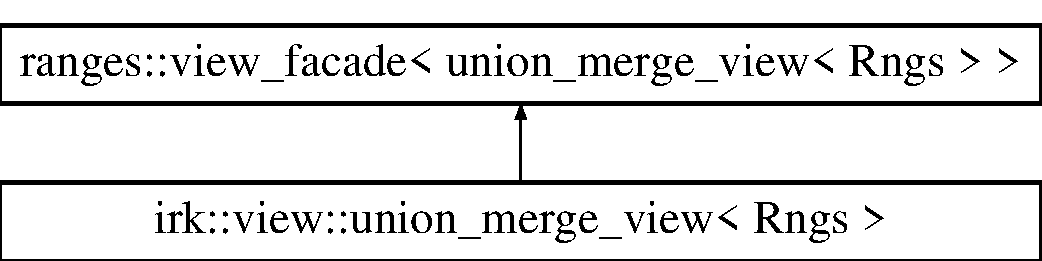
\includegraphics[height=2.000000cm]{classirk_1_1view_1_1union__merge__view}
\end{center}
\end{figure}
\subsection*{Public Member Functions}
\begin{DoxyCompactItemize}
\item 
\mbox{\hyperlink{classirk_1_1view_1_1union__merge__view_a67de18521fcdb6d222fddc441fe827de}{union\+\_\+merge\+\_\+view}} ()=default
\item 
\mbox{\hyperlink{classirk_1_1view_1_1union__merge__view_af6199af626f858573667d182400d01ec}{union\+\_\+merge\+\_\+view}} (Rngs rngs)
\end{DoxyCompactItemize}


\subsection{Constructor \& Destructor Documentation}
\mbox{\Hypertarget{classirk_1_1view_1_1union__merge__view_a67de18521fcdb6d222fddc441fe827de}\label{classirk_1_1view_1_1union__merge__view_a67de18521fcdb6d222fddc441fe827de}} 
\index{irk\+::view\+::union\+\_\+merge\+\_\+view@{irk\+::view\+::union\+\_\+merge\+\_\+view}!union\+\_\+merge\+\_\+view@{union\+\_\+merge\+\_\+view}}
\index{union\+\_\+merge\+\_\+view@{union\+\_\+merge\+\_\+view}!irk\+::view\+::union\+\_\+merge\+\_\+view@{irk\+::view\+::union\+\_\+merge\+\_\+view}}
\subsubsection{\texorpdfstring{union\+\_\+merge\+\_\+view()}{union\_merge\_view()}\hspace{0.1cm}{\footnotesize\ttfamily [1/2]}}
{\footnotesize\ttfamily template$<$class Rngs $>$ \\
\mbox{\hyperlink{classirk_1_1view_1_1union__merge__view}{irk\+::view\+::union\+\_\+merge\+\_\+view}}$<$ Rngs $>$\+::\mbox{\hyperlink{classirk_1_1view_1_1union__merge__view}{union\+\_\+merge\+\_\+view}} (\begin{DoxyParamCaption}{ }\end{DoxyParamCaption})\hspace{0.3cm}{\ttfamily [default]}}

\mbox{\Hypertarget{classirk_1_1view_1_1union__merge__view_af6199af626f858573667d182400d01ec}\label{classirk_1_1view_1_1union__merge__view_af6199af626f858573667d182400d01ec}} 
\index{irk\+::view\+::union\+\_\+merge\+\_\+view@{irk\+::view\+::union\+\_\+merge\+\_\+view}!union\+\_\+merge\+\_\+view@{union\+\_\+merge\+\_\+view}}
\index{union\+\_\+merge\+\_\+view@{union\+\_\+merge\+\_\+view}!irk\+::view\+::union\+\_\+merge\+\_\+view@{irk\+::view\+::union\+\_\+merge\+\_\+view}}
\subsubsection{\texorpdfstring{union\+\_\+merge\+\_\+view()}{union\_merge\_view()}\hspace{0.1cm}{\footnotesize\ttfamily [2/2]}}
{\footnotesize\ttfamily template$<$class Rngs $>$ \\
\mbox{\hyperlink{classirk_1_1view_1_1union__merge__view}{irk\+::view\+::union\+\_\+merge\+\_\+view}}$<$ Rngs $>$\+::\mbox{\hyperlink{classirk_1_1view_1_1union__merge__view}{union\+\_\+merge\+\_\+view}} (\begin{DoxyParamCaption}\item[{Rngs}]{rngs }\end{DoxyParamCaption})\hspace{0.3cm}{\ttfamily [inline]}, {\ttfamily [explicit]}}



The documentation for this class was generated from the following file\+:\begin{DoxyCompactItemize}
\item 
include/irkit/\mbox{\hyperlink{view_8hpp}{view.\+hpp}}\end{DoxyCompactItemize}

\hypertarget{classirk_1_1union__range}{}\section{irk\+:\+:union\+\_\+range$<$ Range $>$ Class Template Reference}
\label{classirk_1_1union__range}\index{irk\+::union\+\_\+range$<$ Range $>$@{irk\+::union\+\_\+range$<$ Range $>$}}


Represents a union of sorted ranges (e.\+g., posting lists).  




{\ttfamily \#include $<$unionrange.\+hpp$>$}

\subsection*{Classes}
\begin{DoxyCompactItemize}
\item 
struct \mbox{\hyperlink{structirk_1_1union__range_1_1docterm}{docterm}}
\begin{DoxyCompactList}\small\item\em Pair of document ID and term ID to use in D\+A\+AT term heap. \end{DoxyCompactList}\end{DoxyCompactItemize}
\subsection*{Public Types}
\begin{DoxyCompactItemize}
\item 
using \mbox{\hyperlink{classirk_1_1union__range_aae1621f1e73b1b78990ad11eaa52452b}{range\+\_\+type}} = Range
\item 
using \mbox{\hyperlink{classirk_1_1union__range_ac125c83e17d473ee5480fef76cfe42f9}{posting\+\_\+type}} = \mbox{\hyperlink{namespaceirk_a1e48b43a3f40d553264380da5e7263c1}{pure\+\_\+element\+\_\+t}}$<$ \mbox{\hyperlink{classirk_1_1union__range_aae1621f1e73b1b78990ad11eaa52452b}{range\+\_\+type}} $>$
\item 
using \mbox{\hyperlink{classirk_1_1union__range_af728218b976df464ebb051a9e5358e93}{score\+\_\+type}} = \mbox{\hyperlink{namespaceirk_a87bce44d1e3fdff0b1b3bb78f2a5f924}{score\+\_\+t}}$<$ \mbox{\hyperlink{classirk_1_1union__range_ac125c83e17d473ee5480fef76cfe42f9}{posting\+\_\+type}} $>$
\item 
using \mbox{\hyperlink{classirk_1_1union__range_aa502a10f2f5c682199072c0ba11a77a9}{doc\+\_\+type}} = \mbox{\hyperlink{namespaceirk_af5d95ec091f3bd711790e71ccb533903}{doc\+\_\+t}}$<$ \mbox{\hyperlink{classirk_1_1union__range_ac125c83e17d473ee5480fef76cfe42f9}{posting\+\_\+type}} $>$
\end{DoxyCompactItemize}
\subsection*{Public Member Functions}
\begin{DoxyCompactItemize}
\item 
\mbox{\hyperlink{classirk_1_1union__range_a64113cb12f111b46248be984b3ca16c2}{union\+\_\+range}} (const std\+::vector$<$ \mbox{\hyperlink{classirk_1_1union__range_aae1621f1e73b1b78990ad11eaa52452b}{range\+\_\+type}} $>$ \&query\+\_\+postings, const std\+::vector$<$ \mbox{\hyperlink{classirk_1_1union__range_af728218b976df464ebb051a9e5358e93}{score\+\_\+type}} $>$ \&weights, const std\+::vector$<$ \mbox{\hyperlink{classirk_1_1union__range_af728218b976df464ebb051a9e5358e93}{score\+\_\+type}} $>$ \&max\+\_\+scores=std\+::move(std\+::vector$<$ \mbox{\hyperlink{classirk_1_1union__range_af728218b976df464ebb051a9e5358e93}{score\+\_\+type}} $>$()))
\begin{DoxyCompactList}\small\item\em Creates new union range from posting lists and term weights. \end{DoxyCompactList}\item 
unsigned int \mbox{\hyperlink{classirk_1_1union__range_a0b771d0ee6fb2ac3c04be8a2d2d47b33}{peek\+\_\+term}} ()
\begin{DoxyCompactList}\small\item\em Returns the next posting\textquotesingle{}s term without advancing to the next one. \end{DoxyCompactList}\item 
\mbox{\hyperlink{classirk_1_1union__range_ac125c83e17d473ee5480fef76cfe42f9}{posting\+\_\+type}} \mbox{\hyperlink{classirk_1_1union__range_a634d96d13219c2856a6bedf37cd8f1de}{peek\+\_\+posting}} ()
\begin{DoxyCompactList}\small\item\em Returns the next posting without advancing to the next one. \end{DoxyCompactList}\item 
\mbox{\hyperlink{classirk_1_1union__range_ac125c83e17d473ee5480fef76cfe42f9}{posting\+\_\+type}} \mbox{\hyperlink{classirk_1_1union__range_a3513c7a28c0e241a6f9ccfc5bf7b6e67}{next\+\_\+posting}} ()
\begin{DoxyCompactList}\small\item\em Returns the next posting in sorted union order. \end{DoxyCompactList}\item 
\mbox{\hyperlink{classirk_1_1union__range_ac125c83e17d473ee5480fef76cfe42f9}{posting\+\_\+type}} \mbox{\hyperlink{classirk_1_1union__range_a8c5c42595554997abba7ce81c4e8251a}{next\+\_\+doc}} ()
\begin{DoxyCompactList}\small\item\em Returns the next {\itshape accumulated posting} in sorted union order. \end{DoxyCompactList}\item 
std\+::vector$<$ \mbox{\hyperlink{structirk_1_1union__range_1_1docterm}{docterm}} $>$ \mbox{\hyperlink{classirk_1_1union__range_a55d2c36c722c0d865783188eb8e9c584}{select\+\_\+pivot}} (\mbox{\hyperlink{classirk_1_1union__range_af728218b976df464ebb051a9e5358e93}{score\+\_\+type}} threshold)
\item 
\mbox{\hyperlink{classirk_1_1union__range_ac125c83e17d473ee5480fef76cfe42f9}{posting\+\_\+type}} \mbox{\hyperlink{classirk_1_1union__range_a230fb4a5ca924c3d7407baec393c53b7}{next\+\_\+doc\+\_\+wand}} (\mbox{\hyperlink{classirk_1_1union__range_af728218b976df464ebb051a9e5358e93}{score\+\_\+type}} threshold)
\item 
bool \mbox{\hyperlink{classirk_1_1union__range_a661cc5c6767ecd8b468e5b13fb6460f5}{empty}} () const
\begin{DoxyCompactList}\small\item\em Returns true if no further postings are available. \end{DoxyCompactList}\end{DoxyCompactItemize}
\subsection*{Protected Member Functions}
\begin{DoxyCompactItemize}
\item 
void \mbox{\hyperlink{classirk_1_1union__range_a0bd95ecb10bd2f8ee81c5bd23aad3935}{init}} (const std\+::vector$<$ \mbox{\hyperlink{classirk_1_1union__range_aae1621f1e73b1b78990ad11eaa52452b}{range\+\_\+type}} $>$ \&query\+\_\+postings)
\begin{DoxyCompactList}\small\item\em Initilizes moving ranges and heap. \end{DoxyCompactList}\item 
void \mbox{\hyperlink{classirk_1_1union__range_ad195345c32357a6269333a45dd785da8}{nextge}} (unsigned int term, \mbox{\hyperlink{classirk_1_1union__range_aa502a10f2f5c682199072c0ba11a77a9}{doc\+\_\+type}} doc)
\end{DoxyCompactItemize}
\subsection*{Protected Attributes}
\begin{DoxyCompactItemize}
\item 
const std\+::vector$<$ \mbox{\hyperlink{classirk_1_1union__range_af728218b976df464ebb051a9e5358e93}{score\+\_\+type}} $>$ \& \mbox{\hyperlink{classirk_1_1union__range_ad593ed1dc96a2caf524511cb3833910c}{weights\+\_\+}}
\item 
const std\+::vector$<$ \mbox{\hyperlink{classirk_1_1union__range_af728218b976df464ebb051a9e5358e93}{score\+\_\+type}} $>$ \& \mbox{\hyperlink{classirk_1_1union__range_accd3b6fdbaccc21952e2586985f2373e}{max\+\_\+scores\+\_\+}}
\item 
std\+::vector$<$ \mbox{\hyperlink{structirk_1_1moving__range}{moving\+\_\+range}}$<$ \mbox{\hyperlink{namespaceirk_a90f7893fdbf95c6dcc2302148eb0bddb}{const\+\_\+iterator\+\_\+t}}$<$ \mbox{\hyperlink{classirk_1_1union__range_aae1621f1e73b1b78990ad11eaa52452b}{range\+\_\+type}} $>$ $>$ $>$ \mbox{\hyperlink{classirk_1_1union__range_a88706eebcc62dd8386d9ad7042d4af2a}{ranges\+\_\+}}
\item 
std\+::vector$<$ \mbox{\hyperlink{structirk_1_1union__range_1_1docterm}{docterm}} $>$ \mbox{\hyperlink{classirk_1_1union__range_a7f29027760890cf7491bb10753f36b61}{heap\+\_\+}}
\end{DoxyCompactItemize}


\subsection{Detailed Description}
\subsubsection*{template$<$class Range$>$\newline
class irk\+::union\+\_\+range$<$ Range $>$}

Represents a union of sorted ranges (e.\+g., posting lists). 

T\+O\+DO\+:
\begin{DoxyItemize}
\item Generalize.
\item Improve efficiency below 17 ms on Bo\+VW. 
\end{DoxyItemize}

\subsection{Member Typedef Documentation}
\mbox{\Hypertarget{classirk_1_1union__range_aa502a10f2f5c682199072c0ba11a77a9}\label{classirk_1_1union__range_aa502a10f2f5c682199072c0ba11a77a9}} 
\index{irk\+::union\+\_\+range@{irk\+::union\+\_\+range}!doc\+\_\+type@{doc\+\_\+type}}
\index{doc\+\_\+type@{doc\+\_\+type}!irk\+::union\+\_\+range@{irk\+::union\+\_\+range}}
\subsubsection{\texorpdfstring{doc\+\_\+type}{doc\_type}}
{\footnotesize\ttfamily template$<$class Range $>$ \\
using \mbox{\hyperlink{classirk_1_1union__range}{irk\+::union\+\_\+range}}$<$ Range $>$\+::\mbox{\hyperlink{classirk_1_1union__range_aa502a10f2f5c682199072c0ba11a77a9}{doc\+\_\+type}} =  \mbox{\hyperlink{namespaceirk_af5d95ec091f3bd711790e71ccb533903}{doc\+\_\+t}}$<$\mbox{\hyperlink{classirk_1_1union__range_ac125c83e17d473ee5480fef76cfe42f9}{posting\+\_\+type}}$>$}

\mbox{\Hypertarget{classirk_1_1union__range_ac125c83e17d473ee5480fef76cfe42f9}\label{classirk_1_1union__range_ac125c83e17d473ee5480fef76cfe42f9}} 
\index{irk\+::union\+\_\+range@{irk\+::union\+\_\+range}!posting\+\_\+type@{posting\+\_\+type}}
\index{posting\+\_\+type@{posting\+\_\+type}!irk\+::union\+\_\+range@{irk\+::union\+\_\+range}}
\subsubsection{\texorpdfstring{posting\+\_\+type}{posting\_type}}
{\footnotesize\ttfamily template$<$class Range $>$ \\
using \mbox{\hyperlink{classirk_1_1union__range}{irk\+::union\+\_\+range}}$<$ Range $>$\+::\mbox{\hyperlink{classirk_1_1union__range_ac125c83e17d473ee5480fef76cfe42f9}{posting\+\_\+type}} =  \mbox{\hyperlink{namespaceirk_a1e48b43a3f40d553264380da5e7263c1}{pure\+\_\+element\+\_\+t}}$<$\mbox{\hyperlink{classirk_1_1union__range_aae1621f1e73b1b78990ad11eaa52452b}{range\+\_\+type}}$>$}

\mbox{\Hypertarget{classirk_1_1union__range_aae1621f1e73b1b78990ad11eaa52452b}\label{classirk_1_1union__range_aae1621f1e73b1b78990ad11eaa52452b}} 
\index{irk\+::union\+\_\+range@{irk\+::union\+\_\+range}!range\+\_\+type@{range\+\_\+type}}
\index{range\+\_\+type@{range\+\_\+type}!irk\+::union\+\_\+range@{irk\+::union\+\_\+range}}
\subsubsection{\texorpdfstring{range\+\_\+type}{range\_type}}
{\footnotesize\ttfamily template$<$class Range $>$ \\
using \mbox{\hyperlink{classirk_1_1union__range}{irk\+::union\+\_\+range}}$<$ Range $>$\+::\mbox{\hyperlink{classirk_1_1union__range_aae1621f1e73b1b78990ad11eaa52452b}{range\+\_\+type}} =  Range}

\mbox{\Hypertarget{classirk_1_1union__range_af728218b976df464ebb051a9e5358e93}\label{classirk_1_1union__range_af728218b976df464ebb051a9e5358e93}} 
\index{irk\+::union\+\_\+range@{irk\+::union\+\_\+range}!score\+\_\+type@{score\+\_\+type}}
\index{score\+\_\+type@{score\+\_\+type}!irk\+::union\+\_\+range@{irk\+::union\+\_\+range}}
\subsubsection{\texorpdfstring{score\+\_\+type}{score\_type}}
{\footnotesize\ttfamily template$<$class Range $>$ \\
using \mbox{\hyperlink{classirk_1_1union__range}{irk\+::union\+\_\+range}}$<$ Range $>$\+::\mbox{\hyperlink{classirk_1_1union__range_af728218b976df464ebb051a9e5358e93}{score\+\_\+type}} =  \mbox{\hyperlink{namespaceirk_a87bce44d1e3fdff0b1b3bb78f2a5f924}{score\+\_\+t}}$<$\mbox{\hyperlink{classirk_1_1union__range_ac125c83e17d473ee5480fef76cfe42f9}{posting\+\_\+type}}$>$}



\subsection{Constructor \& Destructor Documentation}
\mbox{\Hypertarget{classirk_1_1union__range_a64113cb12f111b46248be984b3ca16c2}\label{classirk_1_1union__range_a64113cb12f111b46248be984b3ca16c2}} 
\index{irk\+::union\+\_\+range@{irk\+::union\+\_\+range}!union\+\_\+range@{union\+\_\+range}}
\index{union\+\_\+range@{union\+\_\+range}!irk\+::union\+\_\+range@{irk\+::union\+\_\+range}}
\subsubsection{\texorpdfstring{union\+\_\+range()}{union\_range()}}
{\footnotesize\ttfamily template$<$class Range $>$ \\
\mbox{\hyperlink{classirk_1_1union__range}{irk\+::union\+\_\+range}}$<$ Range $>$\+::\mbox{\hyperlink{classirk_1_1union__range}{union\+\_\+range}} (\begin{DoxyParamCaption}\item[{const std\+::vector$<$ \mbox{\hyperlink{classirk_1_1union__range_aae1621f1e73b1b78990ad11eaa52452b}{range\+\_\+type}} $>$ \&}]{query\+\_\+postings,  }\item[{const std\+::vector$<$ \mbox{\hyperlink{classirk_1_1union__range_af728218b976df464ebb051a9e5358e93}{score\+\_\+type}} $>$ \&}]{weights,  }\item[{const std\+::vector$<$ \mbox{\hyperlink{classirk_1_1union__range_af728218b976df464ebb051a9e5358e93}{score\+\_\+type}} $>$ \&}]{max\+\_\+scores = {\ttfamily std\+:\+:move(~~~~~~~~~~~~std\+:\+:vector$<$\mbox{\hyperlink{classirk_1_1union__range_af728218b976df464ebb051a9e5358e93}{score\+\_\+type}}$>$())} }\end{DoxyParamCaption})\hspace{0.3cm}{\ttfamily [inline]}}



Creates new union range from posting lists and term weights. 

\begin{DoxyPrecond}{Precondition}
Each posting list must be sorted by increasing document I\+Ds. 
\end{DoxyPrecond}

\begin{DoxyParams}{Parameters}
{\em query\+\_\+postings} & a vector of posting lists for all query terms \\
\hline
{\em weights} & a vector of term weights \\
\hline
\end{DoxyParams}


\subsection{Member Function Documentation}
\mbox{\Hypertarget{classirk_1_1union__range_a661cc5c6767ecd8b468e5b13fb6460f5}\label{classirk_1_1union__range_a661cc5c6767ecd8b468e5b13fb6460f5}} 
\index{irk\+::union\+\_\+range@{irk\+::union\+\_\+range}!empty@{empty}}
\index{empty@{empty}!irk\+::union\+\_\+range@{irk\+::union\+\_\+range}}
\subsubsection{\texorpdfstring{empty()}{empty()}}
{\footnotesize\ttfamily template$<$class Range $>$ \\
bool \mbox{\hyperlink{classirk_1_1union__range}{irk\+::union\+\_\+range}}$<$ Range $>$\+::empty (\begin{DoxyParamCaption}{ }\end{DoxyParamCaption}) const\hspace{0.3cm}{\ttfamily [inline]}}



Returns true if no further postings are available. 

\mbox{\Hypertarget{classirk_1_1union__range_a0bd95ecb10bd2f8ee81c5bd23aad3935}\label{classirk_1_1union__range_a0bd95ecb10bd2f8ee81c5bd23aad3935}} 
\index{irk\+::union\+\_\+range@{irk\+::union\+\_\+range}!init@{init}}
\index{init@{init}!irk\+::union\+\_\+range@{irk\+::union\+\_\+range}}
\subsubsection{\texorpdfstring{init()}{init()}}
{\footnotesize\ttfamily template$<$class Range $>$ \\
void \mbox{\hyperlink{classirk_1_1union__range}{irk\+::union\+\_\+range}}$<$ Range $>$\+::init (\begin{DoxyParamCaption}\item[{const std\+::vector$<$ \mbox{\hyperlink{classirk_1_1union__range_aae1621f1e73b1b78990ad11eaa52452b}{range\+\_\+type}} $>$ \&}]{query\+\_\+postings }\end{DoxyParamCaption})\hspace{0.3cm}{\ttfamily [inline]}, {\ttfamily [protected]}}



Initilizes moving ranges and heap. 

\mbox{\Hypertarget{classirk_1_1union__range_a8c5c42595554997abba7ce81c4e8251a}\label{classirk_1_1union__range_a8c5c42595554997abba7ce81c4e8251a}} 
\index{irk\+::union\+\_\+range@{irk\+::union\+\_\+range}!next\+\_\+doc@{next\+\_\+doc}}
\index{next\+\_\+doc@{next\+\_\+doc}!irk\+::union\+\_\+range@{irk\+::union\+\_\+range}}
\subsubsection{\texorpdfstring{next\+\_\+doc()}{next\_doc()}}
{\footnotesize\ttfamily template$<$class Range $>$ \\
\mbox{\hyperlink{classirk_1_1union__range_ac125c83e17d473ee5480fef76cfe42f9}{posting\+\_\+type}} \mbox{\hyperlink{classirk_1_1union__range}{irk\+::union\+\_\+range}}$<$ Range $>$\+::next\+\_\+doc (\begin{DoxyParamCaption}{ }\end{DoxyParamCaption})\hspace{0.3cm}{\ttfamily [inline]}}



Returns the next {\itshape accumulated posting} in sorted union order. 

An accumulated posting is an object of the same type as posting, but its score is a sum of all the partial scores for the next available document.

Note that if {\itshape next\+\_\+posting} is invoked independently, this will either return an incorrect score or will skip a document (or documents). \mbox{\Hypertarget{classirk_1_1union__range_a230fb4a5ca924c3d7407baec393c53b7}\label{classirk_1_1union__range_a230fb4a5ca924c3d7407baec393c53b7}} 
\index{irk\+::union\+\_\+range@{irk\+::union\+\_\+range}!next\+\_\+doc\+\_\+wand@{next\+\_\+doc\+\_\+wand}}
\index{next\+\_\+doc\+\_\+wand@{next\+\_\+doc\+\_\+wand}!irk\+::union\+\_\+range@{irk\+::union\+\_\+range}}
\subsubsection{\texorpdfstring{next\+\_\+doc\+\_\+wand()}{next\_doc\_wand()}}
{\footnotesize\ttfamily template$<$class Range $>$ \\
\mbox{\hyperlink{classirk_1_1union__range_ac125c83e17d473ee5480fef76cfe42f9}{posting\+\_\+type}} \mbox{\hyperlink{classirk_1_1union__range}{irk\+::union\+\_\+range}}$<$ Range $>$\+::next\+\_\+doc\+\_\+wand (\begin{DoxyParamCaption}\item[{\mbox{\hyperlink{classirk_1_1union__range_af728218b976df464ebb051a9e5358e93}{score\+\_\+type}}}]{threshold }\end{DoxyParamCaption})\hspace{0.3cm}{\ttfamily [inline]}}

\mbox{\Hypertarget{classirk_1_1union__range_a3513c7a28c0e241a6f9ccfc5bf7b6e67}\label{classirk_1_1union__range_a3513c7a28c0e241a6f9ccfc5bf7b6e67}} 
\index{irk\+::union\+\_\+range@{irk\+::union\+\_\+range}!next\+\_\+posting@{next\+\_\+posting}}
\index{next\+\_\+posting@{next\+\_\+posting}!irk\+::union\+\_\+range@{irk\+::union\+\_\+range}}
\subsubsection{\texorpdfstring{next\+\_\+posting()}{next\_posting()}}
{\footnotesize\ttfamily template$<$class Range $>$ \\
\mbox{\hyperlink{classirk_1_1union__range_ac125c83e17d473ee5480fef76cfe42f9}{posting\+\_\+type}} \mbox{\hyperlink{classirk_1_1union__range}{irk\+::union\+\_\+range}}$<$ Range $>$\+::next\+\_\+posting (\begin{DoxyParamCaption}{ }\end{DoxyParamCaption})\hspace{0.3cm}{\ttfamily [inline]}}



Returns the next posting in sorted union order. 

\mbox{\Hypertarget{classirk_1_1union__range_ad195345c32357a6269333a45dd785da8}\label{classirk_1_1union__range_ad195345c32357a6269333a45dd785da8}} 
\index{irk\+::union\+\_\+range@{irk\+::union\+\_\+range}!nextge@{nextge}}
\index{nextge@{nextge}!irk\+::union\+\_\+range@{irk\+::union\+\_\+range}}
\subsubsection{\texorpdfstring{nextge()}{nextge()}}
{\footnotesize\ttfamily template$<$class Range $>$ \\
void \mbox{\hyperlink{classirk_1_1union__range}{irk\+::union\+\_\+range}}$<$ Range $>$\+::nextge (\begin{DoxyParamCaption}\item[{unsigned int}]{term,  }\item[{\mbox{\hyperlink{classirk_1_1union__range_aa502a10f2f5c682199072c0ba11a77a9}{doc\+\_\+type}}}]{doc }\end{DoxyParamCaption})\hspace{0.3cm}{\ttfamily [inline]}, {\ttfamily [protected]}}

\mbox{\Hypertarget{classirk_1_1union__range_a634d96d13219c2856a6bedf37cd8f1de}\label{classirk_1_1union__range_a634d96d13219c2856a6bedf37cd8f1de}} 
\index{irk\+::union\+\_\+range@{irk\+::union\+\_\+range}!peek\+\_\+posting@{peek\+\_\+posting}}
\index{peek\+\_\+posting@{peek\+\_\+posting}!irk\+::union\+\_\+range@{irk\+::union\+\_\+range}}
\subsubsection{\texorpdfstring{peek\+\_\+posting()}{peek\_posting()}}
{\footnotesize\ttfamily template$<$class Range $>$ \\
\mbox{\hyperlink{classirk_1_1union__range_ac125c83e17d473ee5480fef76cfe42f9}{posting\+\_\+type}} \mbox{\hyperlink{classirk_1_1union__range}{irk\+::union\+\_\+range}}$<$ Range $>$\+::peek\+\_\+posting (\begin{DoxyParamCaption}{ }\end{DoxyParamCaption})\hspace{0.3cm}{\ttfamily [inline]}}



Returns the next posting without advancing to the next one. 

\mbox{\Hypertarget{classirk_1_1union__range_a0b771d0ee6fb2ac3c04be8a2d2d47b33}\label{classirk_1_1union__range_a0b771d0ee6fb2ac3c04be8a2d2d47b33}} 
\index{irk\+::union\+\_\+range@{irk\+::union\+\_\+range}!peek\+\_\+term@{peek\+\_\+term}}
\index{peek\+\_\+term@{peek\+\_\+term}!irk\+::union\+\_\+range@{irk\+::union\+\_\+range}}
\subsubsection{\texorpdfstring{peek\+\_\+term()}{peek\_term()}}
{\footnotesize\ttfamily template$<$class Range $>$ \\
unsigned int \mbox{\hyperlink{classirk_1_1union__range}{irk\+::union\+\_\+range}}$<$ Range $>$\+::peek\+\_\+term (\begin{DoxyParamCaption}{ }\end{DoxyParamCaption})\hspace{0.3cm}{\ttfamily [inline]}}



Returns the next posting\textquotesingle{}s term without advancing to the next one. 

\mbox{\Hypertarget{classirk_1_1union__range_a55d2c36c722c0d865783188eb8e9c584}\label{classirk_1_1union__range_a55d2c36c722c0d865783188eb8e9c584}} 
\index{irk\+::union\+\_\+range@{irk\+::union\+\_\+range}!select\+\_\+pivot@{select\+\_\+pivot}}
\index{select\+\_\+pivot@{select\+\_\+pivot}!irk\+::union\+\_\+range@{irk\+::union\+\_\+range}}
\subsubsection{\texorpdfstring{select\+\_\+pivot()}{select\_pivot()}}
{\footnotesize\ttfamily template$<$class Range $>$ \\
std\+::vector$<$\mbox{\hyperlink{structirk_1_1union__range_1_1docterm}{docterm}}$>$ \mbox{\hyperlink{classirk_1_1union__range}{irk\+::union\+\_\+range}}$<$ Range $>$\+::select\+\_\+pivot (\begin{DoxyParamCaption}\item[{\mbox{\hyperlink{classirk_1_1union__range_af728218b976df464ebb051a9e5358e93}{score\+\_\+type}}}]{threshold }\end{DoxyParamCaption})\hspace{0.3cm}{\ttfamily [inline]}}

Returns the docterm entries for all terms preceding (and including) pivot. 

\subsection{Member Data Documentation}
\mbox{\Hypertarget{classirk_1_1union__range_a7f29027760890cf7491bb10753f36b61}\label{classirk_1_1union__range_a7f29027760890cf7491bb10753f36b61}} 
\index{irk\+::union\+\_\+range@{irk\+::union\+\_\+range}!heap\+\_\+@{heap\+\_\+}}
\index{heap\+\_\+@{heap\+\_\+}!irk\+::union\+\_\+range@{irk\+::union\+\_\+range}}
\subsubsection{\texorpdfstring{heap\+\_\+}{heap\_}}
{\footnotesize\ttfamily template$<$class Range $>$ \\
std\+::vector$<$\mbox{\hyperlink{structirk_1_1union__range_1_1docterm}{docterm}}$>$ \mbox{\hyperlink{classirk_1_1union__range}{irk\+::union\+\_\+range}}$<$ Range $>$\+::heap\+\_\+\hspace{0.3cm}{\ttfamily [protected]}}

\mbox{\Hypertarget{classirk_1_1union__range_accd3b6fdbaccc21952e2586985f2373e}\label{classirk_1_1union__range_accd3b6fdbaccc21952e2586985f2373e}} 
\index{irk\+::union\+\_\+range@{irk\+::union\+\_\+range}!max\+\_\+scores\+\_\+@{max\+\_\+scores\+\_\+}}
\index{max\+\_\+scores\+\_\+@{max\+\_\+scores\+\_\+}!irk\+::union\+\_\+range@{irk\+::union\+\_\+range}}
\subsubsection{\texorpdfstring{max\+\_\+scores\+\_\+}{max\_scores\_}}
{\footnotesize\ttfamily template$<$class Range $>$ \\
const std\+::vector$<$\mbox{\hyperlink{classirk_1_1union__range_af728218b976df464ebb051a9e5358e93}{score\+\_\+type}}$>$\& \mbox{\hyperlink{classirk_1_1union__range}{irk\+::union\+\_\+range}}$<$ Range $>$\+::max\+\_\+scores\+\_\+\hspace{0.3cm}{\ttfamily [protected]}}

\mbox{\Hypertarget{classirk_1_1union__range_a88706eebcc62dd8386d9ad7042d4af2a}\label{classirk_1_1union__range_a88706eebcc62dd8386d9ad7042d4af2a}} 
\index{irk\+::union\+\_\+range@{irk\+::union\+\_\+range}!ranges\+\_\+@{ranges\+\_\+}}
\index{ranges\+\_\+@{ranges\+\_\+}!irk\+::union\+\_\+range@{irk\+::union\+\_\+range}}
\subsubsection{\texorpdfstring{ranges\+\_\+}{ranges\_}}
{\footnotesize\ttfamily template$<$class Range $>$ \\
std\+::vector$<$\mbox{\hyperlink{structirk_1_1moving__range}{moving\+\_\+range}}$<$\mbox{\hyperlink{namespaceirk_a90f7893fdbf95c6dcc2302148eb0bddb}{const\+\_\+iterator\+\_\+t}}$<$\mbox{\hyperlink{classirk_1_1union__range_aae1621f1e73b1b78990ad11eaa52452b}{range\+\_\+type}}$>$ $>$ $>$ \mbox{\hyperlink{classirk_1_1union__range}{irk\+::union\+\_\+range}}$<$ Range $>$\+::ranges\+\_\+\hspace{0.3cm}{\ttfamily [protected]}}

\mbox{\Hypertarget{classirk_1_1union__range_ad593ed1dc96a2caf524511cb3833910c}\label{classirk_1_1union__range_ad593ed1dc96a2caf524511cb3833910c}} 
\index{irk\+::union\+\_\+range@{irk\+::union\+\_\+range}!weights\+\_\+@{weights\+\_\+}}
\index{weights\+\_\+@{weights\+\_\+}!irk\+::union\+\_\+range@{irk\+::union\+\_\+range}}
\subsubsection{\texorpdfstring{weights\+\_\+}{weights\_}}
{\footnotesize\ttfamily template$<$class Range $>$ \\
const std\+::vector$<$\mbox{\hyperlink{classirk_1_1union__range_af728218b976df464ebb051a9e5358e93}{score\+\_\+type}}$>$\& \mbox{\hyperlink{classirk_1_1union__range}{irk\+::union\+\_\+range}}$<$ Range $>$\+::weights\+\_\+\hspace{0.3cm}{\ttfamily [protected]}}



The documentation for this class was generated from the following file\+:\begin{DoxyCompactItemize}
\item 
include/irkit/\mbox{\hyperlink{unionrange_8hpp}{unionrange.\+hpp}}\end{DoxyCompactItemize}

\hypertarget{structvalid__scoring__function}{}\section{valid\+\_\+scoring\+\_\+function Struct Reference}
\label{structvalid__scoring__function}\index{valid\+\_\+scoring\+\_\+function@{valid\+\_\+scoring\+\_\+function}}
\subsection*{Public Member Functions}
\begin{DoxyCompactItemize}
\item 
std\+::string \mbox{\hyperlink{structvalid__scoring__function_a39a04cce7c1ee763e79441b9edd47038}{operator()}} (const std\+::string \&scorer)
\end{DoxyCompactItemize}
\subsection*{Public Attributes}
\begin{DoxyCompactItemize}
\item 
std\+::unordered\+\_\+set$<$ std\+::string $>$ \mbox{\hyperlink{structvalid__scoring__function_a0beb8d648a26285eeb98019828b90ed1}{available\+\_\+scorers}}
\end{DoxyCompactItemize}


\subsection{Member Function Documentation}
\mbox{\Hypertarget{structvalid__scoring__function_a39a04cce7c1ee763e79441b9edd47038}\label{structvalid__scoring__function_a39a04cce7c1ee763e79441b9edd47038}} 
\index{valid\+\_\+scoring\+\_\+function@{valid\+\_\+scoring\+\_\+function}!operator()@{operator()}}
\index{operator()@{operator()}!valid\+\_\+scoring\+\_\+function@{valid\+\_\+scoring\+\_\+function}}
\subsubsection{\texorpdfstring{operator()()}{operator()()}}
{\footnotesize\ttfamily std\+::string valid\+\_\+scoring\+\_\+function\+::operator() (\begin{DoxyParamCaption}\item[{const std\+::string \&}]{scorer }\end{DoxyParamCaption})\hspace{0.3cm}{\ttfamily [inline]}}



\subsection{Member Data Documentation}
\mbox{\Hypertarget{structvalid__scoring__function_a0beb8d648a26285eeb98019828b90ed1}\label{structvalid__scoring__function_a0beb8d648a26285eeb98019828b90ed1}} 
\index{valid\+\_\+scoring\+\_\+function@{valid\+\_\+scoring\+\_\+function}!available\+\_\+scorers@{available\+\_\+scorers}}
\index{available\+\_\+scorers@{available\+\_\+scorers}!valid\+\_\+scoring\+\_\+function@{valid\+\_\+scoring\+\_\+function}}
\subsubsection{\texorpdfstring{available\+\_\+scorers}{available\_scorers}}
{\footnotesize\ttfamily std\+::unordered\+\_\+set$<$std\+::string$>$ valid\+\_\+scoring\+\_\+function\+::available\+\_\+scorers}



The documentation for this struct was generated from the following file\+:\begin{DoxyCompactItemize}
\item 
src/\mbox{\hyperlink{irk-score_8cpp}{irk-\/score.\+cpp}}\end{DoxyCompactItemize}

\hypertarget{structirk_1_1varbyte__codec}{}\section{irk\+:\+:varbyte\+\_\+codec$<$ T $>$ Struct Template Reference}
\label{structirk_1_1varbyte__codec}\index{irk\+::varbyte\+\_\+codec$<$ T $>$@{irk\+::varbyte\+\_\+codec$<$ T $>$}}


Variable-\/\+Byte codec.  




{\ttfamily \#include $<$varbyte.\+hpp$>$}

\subsection*{Public Types}
\begin{DoxyCompactItemize}
\item 
using \mbox{\hyperlink{structirk_1_1varbyte__codec_a362fbaf8b27a38eb23a52a85b1af68ac}{value\+\_\+type}} = T
\end{DoxyCompactItemize}
\subsection*{Public Member Functions}
\begin{DoxyCompactItemize}
\item 
std\+::ostream \& \mbox{\hyperlink{structirk_1_1varbyte__codec_a82d69fd436aa9ea1626ad756cfdb6e88}{encode}} (\mbox{\hyperlink{structirk_1_1varbyte__codec_a362fbaf8b27a38eb23a52a85b1af68ac}{value\+\_\+type}} n, std\+::ostream \&sink) const
\item 
std\+::streamsize \mbox{\hyperlink{structirk_1_1varbyte__codec_aba60747b7941c1f10d104f1cf0778534}{decode}} (std\+::istream \&source, \mbox{\hyperlink{structirk_1_1varbyte__codec_a362fbaf8b27a38eb23a52a85b1af68ac}{value\+\_\+type}} \&n) const
\end{DoxyCompactItemize}


\subsection{Detailed Description}
\subsubsection*{template$<$class T$>$\newline
struct irk\+::varbyte\+\_\+codec$<$ T $>$}

Variable-\/\+Byte codec. 

\subsection{Member Typedef Documentation}
\mbox{\Hypertarget{structirk_1_1varbyte__codec_a362fbaf8b27a38eb23a52a85b1af68ac}\label{structirk_1_1varbyte__codec_a362fbaf8b27a38eb23a52a85b1af68ac}} 
\index{irk\+::varbyte\+\_\+codec@{irk\+::varbyte\+\_\+codec}!value\+\_\+type@{value\+\_\+type}}
\index{value\+\_\+type@{value\+\_\+type}!irk\+::varbyte\+\_\+codec@{irk\+::varbyte\+\_\+codec}}
\subsubsection{\texorpdfstring{value\+\_\+type}{value\_type}}
{\footnotesize\ttfamily template$<$class T$>$ \\
using \mbox{\hyperlink{structirk_1_1varbyte__codec}{irk\+::varbyte\+\_\+codec}}$<$ T $>$\+::\mbox{\hyperlink{structirk_1_1varbyte__codec_a362fbaf8b27a38eb23a52a85b1af68ac}{value\+\_\+type}} =  T}



\subsection{Member Function Documentation}
\mbox{\Hypertarget{structirk_1_1varbyte__codec_aba60747b7941c1f10d104f1cf0778534}\label{structirk_1_1varbyte__codec_aba60747b7941c1f10d104f1cf0778534}} 
\index{irk\+::varbyte\+\_\+codec@{irk\+::varbyte\+\_\+codec}!decode@{decode}}
\index{decode@{decode}!irk\+::varbyte\+\_\+codec@{irk\+::varbyte\+\_\+codec}}
\subsubsection{\texorpdfstring{decode()}{decode()}}
{\footnotesize\ttfamily template$<$class T$>$ \\
std\+::streamsize \mbox{\hyperlink{structirk_1_1varbyte__codec}{irk\+::varbyte\+\_\+codec}}$<$ T $>$\+::decode (\begin{DoxyParamCaption}\item[{std\+::istream \&}]{source,  }\item[{\mbox{\hyperlink{structirk_1_1varbyte__codec_a362fbaf8b27a38eb23a52a85b1af68ac}{value\+\_\+type}} \&}]{n }\end{DoxyParamCaption}) const\hspace{0.3cm}{\ttfamily [inline]}}

\mbox{\Hypertarget{structirk_1_1varbyte__codec_a82d69fd436aa9ea1626ad756cfdb6e88}\label{structirk_1_1varbyte__codec_a82d69fd436aa9ea1626ad756cfdb6e88}} 
\index{irk\+::varbyte\+\_\+codec@{irk\+::varbyte\+\_\+codec}!encode@{encode}}
\index{encode@{encode}!irk\+::varbyte\+\_\+codec@{irk\+::varbyte\+\_\+codec}}
\subsubsection{\texorpdfstring{encode()}{encode()}}
{\footnotesize\ttfamily template$<$class T$>$ \\
std\+::ostream\& \mbox{\hyperlink{structirk_1_1varbyte__codec}{irk\+::varbyte\+\_\+codec}}$<$ T $>$\+::encode (\begin{DoxyParamCaption}\item[{\mbox{\hyperlink{structirk_1_1varbyte__codec_a362fbaf8b27a38eb23a52a85b1af68ac}{value\+\_\+type}}}]{n,  }\item[{std\+::ostream \&}]{sink }\end{DoxyParamCaption}) const\hspace{0.3cm}{\ttfamily [inline]}}



The documentation for this struct was generated from the following file\+:\begin{DoxyCompactItemize}
\item 
include/irkit/coding/\mbox{\hyperlink{varbyte_8hpp}{varbyte.\+hpp}}\end{DoxyCompactItemize}

\hypertarget{classirk_1_1vector__block__iterator}{}\section{irk\+:\+:vector\+\_\+block\+\_\+iterator$<$ ListT, sorted $>$ Class Template Reference}
\label{classirk_1_1vector__block__iterator}\index{irk\+::vector\+\_\+block\+\_\+iterator$<$ List\+T, sorted $>$@{irk\+::vector\+\_\+block\+\_\+iterator$<$ List\+T, sorted $>$}}


{\ttfamily \#include $<$vector\+\_\+inverted\+\_\+list.\+hpp$>$}

Inheritance diagram for irk\+:\+:vector\+\_\+block\+\_\+iterator$<$ ListT, sorted $>$\+:\begin{figure}[H]
\begin{center}
\leavevmode
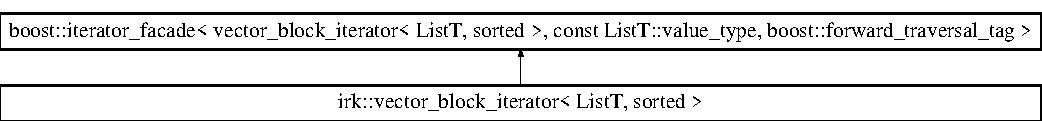
\includegraphics[height=1.627907cm]{classirk_1_1vector__block__iterator}
\end{center}
\end{figure}
\subsection*{Public Types}
\begin{DoxyCompactItemize}
\item 
using \mbox{\hyperlink{classirk_1_1vector__block__iterator_aab9b845032870211b56eddcfd9f8cadb}{view\+\_\+type}} = ListT
\item 
using \mbox{\hyperlink{classirk_1_1vector__block__iterator_a39e5fae2a4258ea1a7cad14a66be2908}{self\+\_\+type}} = \mbox{\hyperlink{classirk_1_1vector__block__iterator}{vector\+\_\+block\+\_\+iterator}}$<$ \mbox{\hyperlink{classirk_1_1vector__block__iterator_aab9b845032870211b56eddcfd9f8cadb}{view\+\_\+type}}, sorted $>$
\item 
using \mbox{\hyperlink{classirk_1_1vector__block__iterator_adc4ee937499f8c9ea24a6f99401b4d22}{difference\+\_\+type}} = int
\item 
using \mbox{\hyperlink{classirk_1_1vector__block__iterator_aaf15da7489a2eb86a95b4c309053e6de}{value\+\_\+type}} = typename List\+T\+::value\+\_\+type
\end{DoxyCompactItemize}
\subsection*{Public Member Functions}
\begin{DoxyCompactItemize}
\item 
\mbox{\hyperlink{classirk_1_1vector__block__iterator_a556c7d699e7aca9bd1980440cee98c4c}{vector\+\_\+block\+\_\+iterator}} ()=default
\item 
\mbox{\hyperlink{classirk_1_1vector__block__iterator_a675b570eae64be69dff0a58aa2e30491}{vector\+\_\+block\+\_\+iterator}} (const \mbox{\hyperlink{classirk_1_1vector__block__iterator_a39e5fae2a4258ea1a7cad14a66be2908}{self\+\_\+type}} \&)=default
\item 
\mbox{\hyperlink{classirk_1_1vector__block__iterator_a7e13b6d84896fcd0c31c090ddd634c45}{vector\+\_\+block\+\_\+iterator}} (const \mbox{\hyperlink{classirk_1_1vector__block__iterator_aab9b845032870211b56eddcfd9f8cadb}{view\+\_\+type}} \&view, \mbox{\hyperlink{classirk_1_1vector__block__iterator_adc4ee937499f8c9ea24a6f99401b4d22}{difference\+\_\+type}} \mbox{\hyperlink{classirk_1_1vector__block__iterator_a820d31edd98d2ecf75daa93efcebd06d}{block}}, \mbox{\hyperlink{classirk_1_1vector__block__iterator_adc4ee937499f8c9ea24a6f99401b4d22}{difference\+\_\+type}} \mbox{\hyperlink{classirk_1_1vector__block__iterator_a886fe6a7ba56c67ca63e0a62e756e1fb}{pos}})
\item 
\mbox{\hyperlink{classirk_1_1vector__block__iterator_a39e5fae2a4258ea1a7cad14a66be2908}{self\+\_\+type}} \& \mbox{\hyperlink{classirk_1_1vector__block__iterator_a698954af3be4c0e65b699141b9b8d0f7}{moveto}} (\mbox{\hyperlink{classirk_1_1vector__block__iterator_aaf15da7489a2eb86a95b4c309053e6de}{value\+\_\+type}} id)
\item 
\mbox{\hyperlink{classirk_1_1vector__block__iterator_a39e5fae2a4258ea1a7cad14a66be2908}{self\+\_\+type}} \mbox{\hyperlink{classirk_1_1vector__block__iterator_acc0471a7ee5d33c78fbbf15ab58e06dc}{nextgeq}} (\mbox{\hyperlink{classirk_1_1vector__block__iterator_aaf15da7489a2eb86a95b4c309053e6de}{value\+\_\+type}} id) const
\item 
{\footnotesize template$<$class Block\+Iterator $>$ }\\\mbox{\hyperlink{classirk_1_1vector__block__iterator_a39e5fae2a4258ea1a7cad14a66be2908}{self\+\_\+type}} \& \mbox{\hyperlink{classirk_1_1vector__block__iterator_a83fd5704ae4a6f65da799890cc203835}{align}} (const Block\+Iterator \&other)
\item 
{\footnotesize template$<$class Block\+Iterator $>$ }\\\mbox{\hyperlink{classirk_1_1vector__block__iterator_a39e5fae2a4258ea1a7cad14a66be2908}{self\+\_\+type}} \mbox{\hyperlink{classirk_1_1vector__block__iterator_af5332945a82553b1af770b7863c2769f}{aligned}} (const Block\+Iterator \&other)
\item 
int \mbox{\hyperlink{classirk_1_1vector__block__iterator_a820d31edd98d2ecf75daa93efcebd06d}{block}} () const
\item 
int \mbox{\hyperlink{classirk_1_1vector__block__iterator_a886fe6a7ba56c67ca63e0a62e756e1fb}{pos}} () const
\end{DoxyCompactItemize}
\subsection*{Friends}
\begin{DoxyCompactItemize}
\item 
class \mbox{\hyperlink{classirk_1_1vector__block__iterator_ac09f73e325921cc50ebcd96bed0f8096}{boost\+::iterator\+\_\+core\+\_\+access}}
\end{DoxyCompactItemize}


\subsection{Member Typedef Documentation}
\mbox{\Hypertarget{classirk_1_1vector__block__iterator_adc4ee937499f8c9ea24a6f99401b4d22}\label{classirk_1_1vector__block__iterator_adc4ee937499f8c9ea24a6f99401b4d22}} 
\index{irk\+::vector\+\_\+block\+\_\+iterator@{irk\+::vector\+\_\+block\+\_\+iterator}!difference\+\_\+type@{difference\+\_\+type}}
\index{difference\+\_\+type@{difference\+\_\+type}!irk\+::vector\+\_\+block\+\_\+iterator@{irk\+::vector\+\_\+block\+\_\+iterator}}
\subsubsection{\texorpdfstring{difference\+\_\+type}{difference\_type}}
{\footnotesize\ttfamily template$<$class ListT , bool sorted$>$ \\
using \mbox{\hyperlink{classirk_1_1vector__block__iterator}{irk\+::vector\+\_\+block\+\_\+iterator}}$<$ ListT, sorted $>$\+::\mbox{\hyperlink{classirk_1_1vector__block__iterator_adc4ee937499f8c9ea24a6f99401b4d22}{difference\+\_\+type}} =  int}

\mbox{\Hypertarget{classirk_1_1vector__block__iterator_a39e5fae2a4258ea1a7cad14a66be2908}\label{classirk_1_1vector__block__iterator_a39e5fae2a4258ea1a7cad14a66be2908}} 
\index{irk\+::vector\+\_\+block\+\_\+iterator@{irk\+::vector\+\_\+block\+\_\+iterator}!self\+\_\+type@{self\+\_\+type}}
\index{self\+\_\+type@{self\+\_\+type}!irk\+::vector\+\_\+block\+\_\+iterator@{irk\+::vector\+\_\+block\+\_\+iterator}}
\subsubsection{\texorpdfstring{self\+\_\+type}{self\_type}}
{\footnotesize\ttfamily template$<$class ListT , bool sorted$>$ \\
using \mbox{\hyperlink{classirk_1_1vector__block__iterator}{irk\+::vector\+\_\+block\+\_\+iterator}}$<$ ListT, sorted $>$\+::\mbox{\hyperlink{classirk_1_1vector__block__iterator_a39e5fae2a4258ea1a7cad14a66be2908}{self\+\_\+type}} =  \mbox{\hyperlink{classirk_1_1vector__block__iterator}{vector\+\_\+block\+\_\+iterator}}$<$\mbox{\hyperlink{classirk_1_1vector__block__iterator_aab9b845032870211b56eddcfd9f8cadb}{view\+\_\+type}}, sorted$>$}

\mbox{\Hypertarget{classirk_1_1vector__block__iterator_aaf15da7489a2eb86a95b4c309053e6de}\label{classirk_1_1vector__block__iterator_aaf15da7489a2eb86a95b4c309053e6de}} 
\index{irk\+::vector\+\_\+block\+\_\+iterator@{irk\+::vector\+\_\+block\+\_\+iterator}!value\+\_\+type@{value\+\_\+type}}
\index{value\+\_\+type@{value\+\_\+type}!irk\+::vector\+\_\+block\+\_\+iterator@{irk\+::vector\+\_\+block\+\_\+iterator}}
\subsubsection{\texorpdfstring{value\+\_\+type}{value\_type}}
{\footnotesize\ttfamily template$<$class ListT , bool sorted$>$ \\
using \mbox{\hyperlink{classirk_1_1vector__block__iterator}{irk\+::vector\+\_\+block\+\_\+iterator}}$<$ ListT, sorted $>$\+::\mbox{\hyperlink{classirk_1_1vector__block__iterator_aaf15da7489a2eb86a95b4c309053e6de}{value\+\_\+type}} =  typename List\+T\+::value\+\_\+type}

\mbox{\Hypertarget{classirk_1_1vector__block__iterator_aab9b845032870211b56eddcfd9f8cadb}\label{classirk_1_1vector__block__iterator_aab9b845032870211b56eddcfd9f8cadb}} 
\index{irk\+::vector\+\_\+block\+\_\+iterator@{irk\+::vector\+\_\+block\+\_\+iterator}!view\+\_\+type@{view\+\_\+type}}
\index{view\+\_\+type@{view\+\_\+type}!irk\+::vector\+\_\+block\+\_\+iterator@{irk\+::vector\+\_\+block\+\_\+iterator}}
\subsubsection{\texorpdfstring{view\+\_\+type}{view\_type}}
{\footnotesize\ttfamily template$<$class ListT , bool sorted$>$ \\
using \mbox{\hyperlink{classirk_1_1vector__block__iterator}{irk\+::vector\+\_\+block\+\_\+iterator}}$<$ ListT, sorted $>$\+::\mbox{\hyperlink{classirk_1_1vector__block__iterator_aab9b845032870211b56eddcfd9f8cadb}{view\+\_\+type}} =  ListT}



\subsection{Constructor \& Destructor Documentation}
\mbox{\Hypertarget{classirk_1_1vector__block__iterator_a556c7d699e7aca9bd1980440cee98c4c}\label{classirk_1_1vector__block__iterator_a556c7d699e7aca9bd1980440cee98c4c}} 
\index{irk\+::vector\+\_\+block\+\_\+iterator@{irk\+::vector\+\_\+block\+\_\+iterator}!vector\+\_\+block\+\_\+iterator@{vector\+\_\+block\+\_\+iterator}}
\index{vector\+\_\+block\+\_\+iterator@{vector\+\_\+block\+\_\+iterator}!irk\+::vector\+\_\+block\+\_\+iterator@{irk\+::vector\+\_\+block\+\_\+iterator}}
\subsubsection{\texorpdfstring{vector\+\_\+block\+\_\+iterator()}{vector\_block\_iterator()}\hspace{0.1cm}{\footnotesize\ttfamily [1/3]}}
{\footnotesize\ttfamily template$<$class ListT , bool sorted$>$ \\
\mbox{\hyperlink{classirk_1_1vector__block__iterator}{irk\+::vector\+\_\+block\+\_\+iterator}}$<$ ListT, sorted $>$\+::\mbox{\hyperlink{classirk_1_1vector__block__iterator}{vector\+\_\+block\+\_\+iterator}} (\begin{DoxyParamCaption}{ }\end{DoxyParamCaption})\hspace{0.3cm}{\ttfamily [default]}}

\mbox{\Hypertarget{classirk_1_1vector__block__iterator_a675b570eae64be69dff0a58aa2e30491}\label{classirk_1_1vector__block__iterator_a675b570eae64be69dff0a58aa2e30491}} 
\index{irk\+::vector\+\_\+block\+\_\+iterator@{irk\+::vector\+\_\+block\+\_\+iterator}!vector\+\_\+block\+\_\+iterator@{vector\+\_\+block\+\_\+iterator}}
\index{vector\+\_\+block\+\_\+iterator@{vector\+\_\+block\+\_\+iterator}!irk\+::vector\+\_\+block\+\_\+iterator@{irk\+::vector\+\_\+block\+\_\+iterator}}
\subsubsection{\texorpdfstring{vector\+\_\+block\+\_\+iterator()}{vector\_block\_iterator()}\hspace{0.1cm}{\footnotesize\ttfamily [2/3]}}
{\footnotesize\ttfamily template$<$class ListT , bool sorted$>$ \\
\mbox{\hyperlink{classirk_1_1vector__block__iterator}{irk\+::vector\+\_\+block\+\_\+iterator}}$<$ ListT, sorted $>$\+::\mbox{\hyperlink{classirk_1_1vector__block__iterator}{vector\+\_\+block\+\_\+iterator}} (\begin{DoxyParamCaption}\item[{const \mbox{\hyperlink{classirk_1_1vector__block__iterator_a39e5fae2a4258ea1a7cad14a66be2908}{self\+\_\+type}} \&}]{ }\end{DoxyParamCaption})\hspace{0.3cm}{\ttfamily [default]}}

\mbox{\Hypertarget{classirk_1_1vector__block__iterator_a7e13b6d84896fcd0c31c090ddd634c45}\label{classirk_1_1vector__block__iterator_a7e13b6d84896fcd0c31c090ddd634c45}} 
\index{irk\+::vector\+\_\+block\+\_\+iterator@{irk\+::vector\+\_\+block\+\_\+iterator}!vector\+\_\+block\+\_\+iterator@{vector\+\_\+block\+\_\+iterator}}
\index{vector\+\_\+block\+\_\+iterator@{vector\+\_\+block\+\_\+iterator}!irk\+::vector\+\_\+block\+\_\+iterator@{irk\+::vector\+\_\+block\+\_\+iterator}}
\subsubsection{\texorpdfstring{vector\+\_\+block\+\_\+iterator()}{vector\_block\_iterator()}\hspace{0.1cm}{\footnotesize\ttfamily [3/3]}}
{\footnotesize\ttfamily template$<$class ListT , bool sorted$>$ \\
\mbox{\hyperlink{classirk_1_1vector__block__iterator}{irk\+::vector\+\_\+block\+\_\+iterator}}$<$ ListT, sorted $>$\+::\mbox{\hyperlink{classirk_1_1vector__block__iterator}{vector\+\_\+block\+\_\+iterator}} (\begin{DoxyParamCaption}\item[{const \mbox{\hyperlink{classirk_1_1vector__block__iterator_aab9b845032870211b56eddcfd9f8cadb}{view\+\_\+type}} \&}]{view,  }\item[{\mbox{\hyperlink{classirk_1_1vector__block__iterator_adc4ee937499f8c9ea24a6f99401b4d22}{difference\+\_\+type}}}]{block,  }\item[{\mbox{\hyperlink{classirk_1_1vector__block__iterator_adc4ee937499f8c9ea24a6f99401b4d22}{difference\+\_\+type}}}]{pos }\end{DoxyParamCaption})\hspace{0.3cm}{\ttfamily [inline]}}



\subsection{Member Function Documentation}
\mbox{\Hypertarget{classirk_1_1vector__block__iterator_a83fd5704ae4a6f65da799890cc203835}\label{classirk_1_1vector__block__iterator_a83fd5704ae4a6f65da799890cc203835}} 
\index{irk\+::vector\+\_\+block\+\_\+iterator@{irk\+::vector\+\_\+block\+\_\+iterator}!align@{align}}
\index{align@{align}!irk\+::vector\+\_\+block\+\_\+iterator@{irk\+::vector\+\_\+block\+\_\+iterator}}
\subsubsection{\texorpdfstring{align()}{align()}}
{\footnotesize\ttfamily template$<$class ListT , bool sorted$>$ \\
template$<$class Block\+Iterator $>$ \\
\mbox{\hyperlink{classirk_1_1vector__block__iterator_a39e5fae2a4258ea1a7cad14a66be2908}{self\+\_\+type}}\& \mbox{\hyperlink{classirk_1_1vector__block__iterator}{irk\+::vector\+\_\+block\+\_\+iterator}}$<$ ListT, sorted $>$\+::align (\begin{DoxyParamCaption}\item[{const Block\+Iterator \&}]{other }\end{DoxyParamCaption})\hspace{0.3cm}{\ttfamily [inline]}}

\mbox{\Hypertarget{classirk_1_1vector__block__iterator_af5332945a82553b1af770b7863c2769f}\label{classirk_1_1vector__block__iterator_af5332945a82553b1af770b7863c2769f}} 
\index{irk\+::vector\+\_\+block\+\_\+iterator@{irk\+::vector\+\_\+block\+\_\+iterator}!aligned@{aligned}}
\index{aligned@{aligned}!irk\+::vector\+\_\+block\+\_\+iterator@{irk\+::vector\+\_\+block\+\_\+iterator}}
\subsubsection{\texorpdfstring{aligned()}{aligned()}}
{\footnotesize\ttfamily template$<$class ListT , bool sorted$>$ \\
template$<$class Block\+Iterator $>$ \\
\mbox{\hyperlink{classirk_1_1vector__block__iterator_a39e5fae2a4258ea1a7cad14a66be2908}{self\+\_\+type}} \mbox{\hyperlink{classirk_1_1vector__block__iterator}{irk\+::vector\+\_\+block\+\_\+iterator}}$<$ ListT, sorted $>$\+::aligned (\begin{DoxyParamCaption}\item[{const Block\+Iterator \&}]{other }\end{DoxyParamCaption})\hspace{0.3cm}{\ttfamily [inline]}}

\mbox{\Hypertarget{classirk_1_1vector__block__iterator_a820d31edd98d2ecf75daa93efcebd06d}\label{classirk_1_1vector__block__iterator_a820d31edd98d2ecf75daa93efcebd06d}} 
\index{irk\+::vector\+\_\+block\+\_\+iterator@{irk\+::vector\+\_\+block\+\_\+iterator}!block@{block}}
\index{block@{block}!irk\+::vector\+\_\+block\+\_\+iterator@{irk\+::vector\+\_\+block\+\_\+iterator}}
\subsubsection{\texorpdfstring{block()}{block()}}
{\footnotesize\ttfamily template$<$class ListT , bool sorted$>$ \\
int \mbox{\hyperlink{classirk_1_1vector__block__iterator}{irk\+::vector\+\_\+block\+\_\+iterator}}$<$ ListT, sorted $>$\+::block (\begin{DoxyParamCaption}{ }\end{DoxyParamCaption}) const\hspace{0.3cm}{\ttfamily [inline]}}

\mbox{\Hypertarget{classirk_1_1vector__block__iterator_a698954af3be4c0e65b699141b9b8d0f7}\label{classirk_1_1vector__block__iterator_a698954af3be4c0e65b699141b9b8d0f7}} 
\index{irk\+::vector\+\_\+block\+\_\+iterator@{irk\+::vector\+\_\+block\+\_\+iterator}!moveto@{moveto}}
\index{moveto@{moveto}!irk\+::vector\+\_\+block\+\_\+iterator@{irk\+::vector\+\_\+block\+\_\+iterator}}
\subsubsection{\texorpdfstring{moveto()}{moveto()}}
{\footnotesize\ttfamily template$<$class ListT , bool sorted$>$ \\
\mbox{\hyperlink{classirk_1_1vector__block__iterator_a39e5fae2a4258ea1a7cad14a66be2908}{self\+\_\+type}}\& \mbox{\hyperlink{classirk_1_1vector__block__iterator}{irk\+::vector\+\_\+block\+\_\+iterator}}$<$ ListT, sorted $>$\+::moveto (\begin{DoxyParamCaption}\item[{\mbox{\hyperlink{classirk_1_1vector__block__iterator_aaf15da7489a2eb86a95b4c309053e6de}{value\+\_\+type}}}]{id }\end{DoxyParamCaption})\hspace{0.3cm}{\ttfamily [inline]}}

\mbox{\Hypertarget{classirk_1_1vector__block__iterator_acc0471a7ee5d33c78fbbf15ab58e06dc}\label{classirk_1_1vector__block__iterator_acc0471a7ee5d33c78fbbf15ab58e06dc}} 
\index{irk\+::vector\+\_\+block\+\_\+iterator@{irk\+::vector\+\_\+block\+\_\+iterator}!nextgeq@{nextgeq}}
\index{nextgeq@{nextgeq}!irk\+::vector\+\_\+block\+\_\+iterator@{irk\+::vector\+\_\+block\+\_\+iterator}}
\subsubsection{\texorpdfstring{nextgeq()}{nextgeq()}}
{\footnotesize\ttfamily template$<$class ListT , bool sorted$>$ \\
\mbox{\hyperlink{classirk_1_1vector__block__iterator_a39e5fae2a4258ea1a7cad14a66be2908}{self\+\_\+type}} \mbox{\hyperlink{classirk_1_1vector__block__iterator}{irk\+::vector\+\_\+block\+\_\+iterator}}$<$ ListT, sorted $>$\+::nextgeq (\begin{DoxyParamCaption}\item[{\mbox{\hyperlink{classirk_1_1vector__block__iterator_aaf15da7489a2eb86a95b4c309053e6de}{value\+\_\+type}}}]{id }\end{DoxyParamCaption}) const\hspace{0.3cm}{\ttfamily [inline]}}

\mbox{\Hypertarget{classirk_1_1vector__block__iterator_a886fe6a7ba56c67ca63e0a62e756e1fb}\label{classirk_1_1vector__block__iterator_a886fe6a7ba56c67ca63e0a62e756e1fb}} 
\index{irk\+::vector\+\_\+block\+\_\+iterator@{irk\+::vector\+\_\+block\+\_\+iterator}!pos@{pos}}
\index{pos@{pos}!irk\+::vector\+\_\+block\+\_\+iterator@{irk\+::vector\+\_\+block\+\_\+iterator}}
\subsubsection{\texorpdfstring{pos()}{pos()}}
{\footnotesize\ttfamily template$<$class ListT , bool sorted$>$ \\
int \mbox{\hyperlink{classirk_1_1vector__block__iterator}{irk\+::vector\+\_\+block\+\_\+iterator}}$<$ ListT, sorted $>$\+::pos (\begin{DoxyParamCaption}{ }\end{DoxyParamCaption}) const\hspace{0.3cm}{\ttfamily [inline]}}



\subsection{Friends And Related Function Documentation}
\mbox{\Hypertarget{classirk_1_1vector__block__iterator_ac09f73e325921cc50ebcd96bed0f8096}\label{classirk_1_1vector__block__iterator_ac09f73e325921cc50ebcd96bed0f8096}} 
\index{irk\+::vector\+\_\+block\+\_\+iterator@{irk\+::vector\+\_\+block\+\_\+iterator}!boost\+::iterator\+\_\+core\+\_\+access@{boost\+::iterator\+\_\+core\+\_\+access}}
\index{boost\+::iterator\+\_\+core\+\_\+access@{boost\+::iterator\+\_\+core\+\_\+access}!irk\+::vector\+\_\+block\+\_\+iterator@{irk\+::vector\+\_\+block\+\_\+iterator}}
\subsubsection{\texorpdfstring{boost\+::iterator\+\_\+core\+\_\+access}{boost::iterator\_core\_access}}
{\footnotesize\ttfamily template$<$class ListT , bool sorted$>$ \\
friend class boost\+::iterator\+\_\+core\+\_\+access\hspace{0.3cm}{\ttfamily [friend]}}



The documentation for this class was generated from the following file\+:\begin{DoxyCompactItemize}
\item 
include/irkit/index/\mbox{\hyperlink{vector__inverted__list_8hpp}{vector\+\_\+inverted\+\_\+list.\+hpp}}\end{DoxyCompactItemize}

\hypertarget{classirk_1_1vector__document__list}{}\section{irk\+:\+:vector\+\_\+document\+\_\+list$<$ T\+Doc $>$ Class Template Reference}
\label{classirk_1_1vector__document__list}\index{irk\+::vector\+\_\+document\+\_\+list$<$ T\+Doc $>$@{irk\+::vector\+\_\+document\+\_\+list$<$ T\+Doc $>$}}


{\ttfamily \#include $<$vector\+\_\+inverted\+\_\+list.\+hpp$>$}

\subsection*{Public Types}
\begin{DoxyCompactItemize}
\item 
using \mbox{\hyperlink{classirk_1_1vector__document__list_ac9387bd9f5dc89b638b6295858a9268c}{size\+\_\+type}} = long
\item 
using \mbox{\hyperlink{classirk_1_1vector__document__list_a0ec9c56f5e12a3a9101b5a18b2fbe69f}{value\+\_\+type}} = T\+Doc
\item 
using \mbox{\hyperlink{classirk_1_1vector__document__list_a8c83c7819e9ffcbb4162d3ee9f41d76a}{self\+\_\+type}} = \mbox{\hyperlink{classirk_1_1vector__document__list}{vector\+\_\+document\+\_\+list}}$<$ T\+Doc $>$
\item 
using \mbox{\hyperlink{classirk_1_1vector__document__list_a42499af78a7d66a1b626858cd424600f}{iterator}} = \mbox{\hyperlink{classirk_1_1vector__block__iterator}{vector\+\_\+block\+\_\+iterator}}$<$ \mbox{\hyperlink{classirk_1_1vector__document__list_a8c83c7819e9ffcbb4162d3ee9f41d76a}{self\+\_\+type}}, true $>$
\item 
using \mbox{\hyperlink{classirk_1_1vector__document__list_a91539ec8ebd87cd47957107df90744aa}{const\+\_\+iterator}} = \mbox{\hyperlink{classirk_1_1vector__document__list_a42499af78a7d66a1b626858cd424600f}{iterator}}
\end{DoxyCompactItemize}
\subsection*{Public Member Functions}
\begin{DoxyCompactItemize}
\item 
\mbox{\hyperlink{classirk_1_1vector__document__list_aee7fc8d2b55075dca80eb883fe5cd0dc}{vector\+\_\+document\+\_\+list}} (std\+::vector$<$ \mbox{\hyperlink{classirk_1_1vector__document__list_a0ec9c56f5e12a3a9101b5a18b2fbe69f}{value\+\_\+type}} $>$ vec)
\item 
\mbox{\hyperlink{classirk_1_1vector__document__list_ac9387bd9f5dc89b638b6295858a9268c}{size\+\_\+type}} \mbox{\hyperlink{classirk_1_1vector__document__list_ad7eac494d9c0aa784efaa1a4faa47616}{size}} () const
\item 
\mbox{\hyperlink{classirk_1_1vector__document__list_ac9387bd9f5dc89b638b6295858a9268c}{size\+\_\+type}} \mbox{\hyperlink{classirk_1_1vector__document__list_ae6a0a3b41d660778ab8dae0e432a47b1}{block\+\_\+size}} () const
\item 
void \mbox{\hyperlink{classirk_1_1vector__document__list_a1e835fe551a310ba89749812b2e9ea1f}{block\+\_\+size}} (\mbox{\hyperlink{classirk_1_1vector__document__list_ac9387bd9f5dc89b638b6295858a9268c}{size\+\_\+type}} block\+\_\+size)
\item 
int \mbox{\hyperlink{classirk_1_1vector__document__list_ab2ab2cef0d517240605010570f7765e8}{num\+\_\+blocks}} () const
\item 
const \mbox{\hyperlink{classirk_1_1vector__document__list_a0ec9c56f5e12a3a9101b5a18b2fbe69f}{value\+\_\+type}} \& \mbox{\hyperlink{classirk_1_1vector__document__list_a005d5854e07f49ade87827544cc88d7f}{operator\mbox{[}$\,$\mbox{]}}} (std\+::size\+\_\+t pos) const
\item 
\mbox{\hyperlink{classirk_1_1vector__document__list_a42499af78a7d66a1b626858cd424600f}{iterator}} \mbox{\hyperlink{classirk_1_1vector__document__list_a014b3737e63a4472e66ccb90a515f340}{begin}} () const
\item 
\mbox{\hyperlink{classirk_1_1vector__document__list_a42499af78a7d66a1b626858cd424600f}{iterator}} \mbox{\hyperlink{classirk_1_1vector__document__list_adafc0267ab0f84e5240011c96efd9681}{end}} () const
\item 
\mbox{\hyperlink{classirk_1_1vector__document__list_a42499af78a7d66a1b626858cd424600f}{iterator}} \mbox{\hyperlink{classirk_1_1vector__document__list_af25b19f3edd8c826dea2c2a8523c2772}{lookup}} (\mbox{\hyperlink{classirk_1_1vector__document__list_a0ec9c56f5e12a3a9101b5a18b2fbe69f}{value\+\_\+type}} id) const
\end{DoxyCompactItemize}


\subsection{Member Typedef Documentation}
\mbox{\Hypertarget{classirk_1_1vector__document__list_a91539ec8ebd87cd47957107df90744aa}\label{classirk_1_1vector__document__list_a91539ec8ebd87cd47957107df90744aa}} 
\index{irk\+::vector\+\_\+document\+\_\+list@{irk\+::vector\+\_\+document\+\_\+list}!const\+\_\+iterator@{const\+\_\+iterator}}
\index{const\+\_\+iterator@{const\+\_\+iterator}!irk\+::vector\+\_\+document\+\_\+list@{irk\+::vector\+\_\+document\+\_\+list}}
\subsubsection{\texorpdfstring{const\+\_\+iterator}{const\_iterator}}
{\footnotesize\ttfamily template$<$class T\+Doc  = long$>$ \\
using \mbox{\hyperlink{classirk_1_1vector__document__list}{irk\+::vector\+\_\+document\+\_\+list}}$<$ T\+Doc $>$\+::\mbox{\hyperlink{classirk_1_1vector__document__list_a91539ec8ebd87cd47957107df90744aa}{const\+\_\+iterator}} =  \mbox{\hyperlink{classirk_1_1vector__document__list_a42499af78a7d66a1b626858cd424600f}{iterator}}}

\mbox{\Hypertarget{classirk_1_1vector__document__list_a42499af78a7d66a1b626858cd424600f}\label{classirk_1_1vector__document__list_a42499af78a7d66a1b626858cd424600f}} 
\index{irk\+::vector\+\_\+document\+\_\+list@{irk\+::vector\+\_\+document\+\_\+list}!iterator@{iterator}}
\index{iterator@{iterator}!irk\+::vector\+\_\+document\+\_\+list@{irk\+::vector\+\_\+document\+\_\+list}}
\subsubsection{\texorpdfstring{iterator}{iterator}}
{\footnotesize\ttfamily template$<$class T\+Doc  = long$>$ \\
using \mbox{\hyperlink{classirk_1_1vector__document__list}{irk\+::vector\+\_\+document\+\_\+list}}$<$ T\+Doc $>$\+::\mbox{\hyperlink{classirk_1_1vector__document__list_a42499af78a7d66a1b626858cd424600f}{iterator}} =  \mbox{\hyperlink{classirk_1_1vector__block__iterator}{vector\+\_\+block\+\_\+iterator}}$<$\mbox{\hyperlink{classirk_1_1vector__document__list_a8c83c7819e9ffcbb4162d3ee9f41d76a}{self\+\_\+type}}, true$>$}

\mbox{\Hypertarget{classirk_1_1vector__document__list_a8c83c7819e9ffcbb4162d3ee9f41d76a}\label{classirk_1_1vector__document__list_a8c83c7819e9ffcbb4162d3ee9f41d76a}} 
\index{irk\+::vector\+\_\+document\+\_\+list@{irk\+::vector\+\_\+document\+\_\+list}!self\+\_\+type@{self\+\_\+type}}
\index{self\+\_\+type@{self\+\_\+type}!irk\+::vector\+\_\+document\+\_\+list@{irk\+::vector\+\_\+document\+\_\+list}}
\subsubsection{\texorpdfstring{self\+\_\+type}{self\_type}}
{\footnotesize\ttfamily template$<$class T\+Doc  = long$>$ \\
using \mbox{\hyperlink{classirk_1_1vector__document__list}{irk\+::vector\+\_\+document\+\_\+list}}$<$ T\+Doc $>$\+::\mbox{\hyperlink{classirk_1_1vector__document__list_a8c83c7819e9ffcbb4162d3ee9f41d76a}{self\+\_\+type}} =  \mbox{\hyperlink{classirk_1_1vector__document__list}{vector\+\_\+document\+\_\+list}}$<$T\+Doc$>$}

\mbox{\Hypertarget{classirk_1_1vector__document__list_ac9387bd9f5dc89b638b6295858a9268c}\label{classirk_1_1vector__document__list_ac9387bd9f5dc89b638b6295858a9268c}} 
\index{irk\+::vector\+\_\+document\+\_\+list@{irk\+::vector\+\_\+document\+\_\+list}!size\+\_\+type@{size\+\_\+type}}
\index{size\+\_\+type@{size\+\_\+type}!irk\+::vector\+\_\+document\+\_\+list@{irk\+::vector\+\_\+document\+\_\+list}}
\subsubsection{\texorpdfstring{size\+\_\+type}{size\_type}}
{\footnotesize\ttfamily template$<$class T\+Doc  = long$>$ \\
using \mbox{\hyperlink{classirk_1_1vector__document__list}{irk\+::vector\+\_\+document\+\_\+list}}$<$ T\+Doc $>$\+::\mbox{\hyperlink{classirk_1_1vector__document__list_ac9387bd9f5dc89b638b6295858a9268c}{size\+\_\+type}} =  long}

\mbox{\Hypertarget{classirk_1_1vector__document__list_a0ec9c56f5e12a3a9101b5a18b2fbe69f}\label{classirk_1_1vector__document__list_a0ec9c56f5e12a3a9101b5a18b2fbe69f}} 
\index{irk\+::vector\+\_\+document\+\_\+list@{irk\+::vector\+\_\+document\+\_\+list}!value\+\_\+type@{value\+\_\+type}}
\index{value\+\_\+type@{value\+\_\+type}!irk\+::vector\+\_\+document\+\_\+list@{irk\+::vector\+\_\+document\+\_\+list}}
\subsubsection{\texorpdfstring{value\+\_\+type}{value\_type}}
{\footnotesize\ttfamily template$<$class T\+Doc  = long$>$ \\
using \mbox{\hyperlink{classirk_1_1vector__document__list}{irk\+::vector\+\_\+document\+\_\+list}}$<$ T\+Doc $>$\+::\mbox{\hyperlink{classirk_1_1vector__document__list_a0ec9c56f5e12a3a9101b5a18b2fbe69f}{value\+\_\+type}} =  T\+Doc}



\subsection{Constructor \& Destructor Documentation}
\mbox{\Hypertarget{classirk_1_1vector__document__list_aee7fc8d2b55075dca80eb883fe5cd0dc}\label{classirk_1_1vector__document__list_aee7fc8d2b55075dca80eb883fe5cd0dc}} 
\index{irk\+::vector\+\_\+document\+\_\+list@{irk\+::vector\+\_\+document\+\_\+list}!vector\+\_\+document\+\_\+list@{vector\+\_\+document\+\_\+list}}
\index{vector\+\_\+document\+\_\+list@{vector\+\_\+document\+\_\+list}!irk\+::vector\+\_\+document\+\_\+list@{irk\+::vector\+\_\+document\+\_\+list}}
\subsubsection{\texorpdfstring{vector\+\_\+document\+\_\+list()}{vector\_document\_list()}}
{\footnotesize\ttfamily template$<$class T\+Doc  = long$>$ \\
\mbox{\hyperlink{classirk_1_1vector__document__list}{irk\+::vector\+\_\+document\+\_\+list}}$<$ T\+Doc $>$\+::\mbox{\hyperlink{classirk_1_1vector__document__list}{vector\+\_\+document\+\_\+list}} (\begin{DoxyParamCaption}\item[{std\+::vector$<$ \mbox{\hyperlink{classirk_1_1vector__document__list_a0ec9c56f5e12a3a9101b5a18b2fbe69f}{value\+\_\+type}} $>$}]{vec }\end{DoxyParamCaption})\hspace{0.3cm}{\ttfamily [inline]}}



\subsection{Member Function Documentation}
\mbox{\Hypertarget{classirk_1_1vector__document__list_a014b3737e63a4472e66ccb90a515f340}\label{classirk_1_1vector__document__list_a014b3737e63a4472e66ccb90a515f340}} 
\index{irk\+::vector\+\_\+document\+\_\+list@{irk\+::vector\+\_\+document\+\_\+list}!begin@{begin}}
\index{begin@{begin}!irk\+::vector\+\_\+document\+\_\+list@{irk\+::vector\+\_\+document\+\_\+list}}
\subsubsection{\texorpdfstring{begin()}{begin()}}
{\footnotesize\ttfamily template$<$class T\+Doc  = long$>$ \\
\mbox{\hyperlink{classirk_1_1vector__document__list_a42499af78a7d66a1b626858cd424600f}{iterator}} \mbox{\hyperlink{classirk_1_1vector__document__list}{irk\+::vector\+\_\+document\+\_\+list}}$<$ T\+Doc $>$\+::begin (\begin{DoxyParamCaption}{ }\end{DoxyParamCaption}) const\hspace{0.3cm}{\ttfamily [inline]}}

\mbox{\Hypertarget{classirk_1_1vector__document__list_ae6a0a3b41d660778ab8dae0e432a47b1}\label{classirk_1_1vector__document__list_ae6a0a3b41d660778ab8dae0e432a47b1}} 
\index{irk\+::vector\+\_\+document\+\_\+list@{irk\+::vector\+\_\+document\+\_\+list}!block\+\_\+size@{block\+\_\+size}}
\index{block\+\_\+size@{block\+\_\+size}!irk\+::vector\+\_\+document\+\_\+list@{irk\+::vector\+\_\+document\+\_\+list}}
\subsubsection{\texorpdfstring{block\+\_\+size()}{block\_size()}\hspace{0.1cm}{\footnotesize\ttfamily [1/2]}}
{\footnotesize\ttfamily template$<$class T\+Doc  = long$>$ \\
\mbox{\hyperlink{classirk_1_1vector__document__list_ac9387bd9f5dc89b638b6295858a9268c}{size\+\_\+type}} \mbox{\hyperlink{classirk_1_1vector__document__list}{irk\+::vector\+\_\+document\+\_\+list}}$<$ T\+Doc $>$\+::block\+\_\+size (\begin{DoxyParamCaption}{ }\end{DoxyParamCaption}) const\hspace{0.3cm}{\ttfamily [inline]}}

\mbox{\Hypertarget{classirk_1_1vector__document__list_a1e835fe551a310ba89749812b2e9ea1f}\label{classirk_1_1vector__document__list_a1e835fe551a310ba89749812b2e9ea1f}} 
\index{irk\+::vector\+\_\+document\+\_\+list@{irk\+::vector\+\_\+document\+\_\+list}!block\+\_\+size@{block\+\_\+size}}
\index{block\+\_\+size@{block\+\_\+size}!irk\+::vector\+\_\+document\+\_\+list@{irk\+::vector\+\_\+document\+\_\+list}}
\subsubsection{\texorpdfstring{block\+\_\+size()}{block\_size()}\hspace{0.1cm}{\footnotesize\ttfamily [2/2]}}
{\footnotesize\ttfamily template$<$class T\+Doc  = long$>$ \\
void \mbox{\hyperlink{classirk_1_1vector__document__list}{irk\+::vector\+\_\+document\+\_\+list}}$<$ T\+Doc $>$\+::block\+\_\+size (\begin{DoxyParamCaption}\item[{\mbox{\hyperlink{classirk_1_1vector__document__list_ac9387bd9f5dc89b638b6295858a9268c}{size\+\_\+type}}}]{block\+\_\+size }\end{DoxyParamCaption})\hspace{0.3cm}{\ttfamily [inline]}}

\mbox{\Hypertarget{classirk_1_1vector__document__list_adafc0267ab0f84e5240011c96efd9681}\label{classirk_1_1vector__document__list_adafc0267ab0f84e5240011c96efd9681}} 
\index{irk\+::vector\+\_\+document\+\_\+list@{irk\+::vector\+\_\+document\+\_\+list}!end@{end}}
\index{end@{end}!irk\+::vector\+\_\+document\+\_\+list@{irk\+::vector\+\_\+document\+\_\+list}}
\subsubsection{\texorpdfstring{end()}{end()}}
{\footnotesize\ttfamily template$<$class T\+Doc  = long$>$ \\
\mbox{\hyperlink{classirk_1_1vector__document__list_a42499af78a7d66a1b626858cd424600f}{iterator}} \mbox{\hyperlink{classirk_1_1vector__document__list}{irk\+::vector\+\_\+document\+\_\+list}}$<$ T\+Doc $>$\+::end (\begin{DoxyParamCaption}{ }\end{DoxyParamCaption}) const\hspace{0.3cm}{\ttfamily [inline]}}

\mbox{\Hypertarget{classirk_1_1vector__document__list_af25b19f3edd8c826dea2c2a8523c2772}\label{classirk_1_1vector__document__list_af25b19f3edd8c826dea2c2a8523c2772}} 
\index{irk\+::vector\+\_\+document\+\_\+list@{irk\+::vector\+\_\+document\+\_\+list}!lookup@{lookup}}
\index{lookup@{lookup}!irk\+::vector\+\_\+document\+\_\+list@{irk\+::vector\+\_\+document\+\_\+list}}
\subsubsection{\texorpdfstring{lookup()}{lookup()}}
{\footnotesize\ttfamily template$<$class T\+Doc  = long$>$ \\
\mbox{\hyperlink{classirk_1_1vector__document__list_a42499af78a7d66a1b626858cd424600f}{iterator}} \mbox{\hyperlink{classirk_1_1vector__document__list}{irk\+::vector\+\_\+document\+\_\+list}}$<$ T\+Doc $>$\+::lookup (\begin{DoxyParamCaption}\item[{\mbox{\hyperlink{classirk_1_1vector__document__list_a0ec9c56f5e12a3a9101b5a18b2fbe69f}{value\+\_\+type}}}]{id }\end{DoxyParamCaption}) const\hspace{0.3cm}{\ttfamily [inline]}}

\mbox{\Hypertarget{classirk_1_1vector__document__list_ab2ab2cef0d517240605010570f7765e8}\label{classirk_1_1vector__document__list_ab2ab2cef0d517240605010570f7765e8}} 
\index{irk\+::vector\+\_\+document\+\_\+list@{irk\+::vector\+\_\+document\+\_\+list}!num\+\_\+blocks@{num\+\_\+blocks}}
\index{num\+\_\+blocks@{num\+\_\+blocks}!irk\+::vector\+\_\+document\+\_\+list@{irk\+::vector\+\_\+document\+\_\+list}}
\subsubsection{\texorpdfstring{num\+\_\+blocks()}{num\_blocks()}}
{\footnotesize\ttfamily template$<$class T\+Doc  = long$>$ \\
int \mbox{\hyperlink{classirk_1_1vector__document__list}{irk\+::vector\+\_\+document\+\_\+list}}$<$ T\+Doc $>$\+::num\+\_\+blocks (\begin{DoxyParamCaption}{ }\end{DoxyParamCaption}) const\hspace{0.3cm}{\ttfamily [inline]}}

\mbox{\Hypertarget{classirk_1_1vector__document__list_a005d5854e07f49ade87827544cc88d7f}\label{classirk_1_1vector__document__list_a005d5854e07f49ade87827544cc88d7f}} 
\index{irk\+::vector\+\_\+document\+\_\+list@{irk\+::vector\+\_\+document\+\_\+list}!operator\mbox{[}\mbox{]}@{operator[]}}
\index{operator\mbox{[}\mbox{]}@{operator[]}!irk\+::vector\+\_\+document\+\_\+list@{irk\+::vector\+\_\+document\+\_\+list}}
\subsubsection{\texorpdfstring{operator[]()}{operator[]()}}
{\footnotesize\ttfamily template$<$class T\+Doc  = long$>$ \\
const \mbox{\hyperlink{classirk_1_1vector__document__list_a0ec9c56f5e12a3a9101b5a18b2fbe69f}{value\+\_\+type}}\& \mbox{\hyperlink{classirk_1_1vector__document__list}{irk\+::vector\+\_\+document\+\_\+list}}$<$ T\+Doc $>$\+::operator\mbox{[}$\,$\mbox{]} (\begin{DoxyParamCaption}\item[{std\+::size\+\_\+t}]{pos }\end{DoxyParamCaption}) const\hspace{0.3cm}{\ttfamily [inline]}}

\mbox{\Hypertarget{classirk_1_1vector__document__list_ad7eac494d9c0aa784efaa1a4faa47616}\label{classirk_1_1vector__document__list_ad7eac494d9c0aa784efaa1a4faa47616}} 
\index{irk\+::vector\+\_\+document\+\_\+list@{irk\+::vector\+\_\+document\+\_\+list}!size@{size}}
\index{size@{size}!irk\+::vector\+\_\+document\+\_\+list@{irk\+::vector\+\_\+document\+\_\+list}}
\subsubsection{\texorpdfstring{size()}{size()}}
{\footnotesize\ttfamily template$<$class T\+Doc  = long$>$ \\
\mbox{\hyperlink{classirk_1_1vector__document__list_ac9387bd9f5dc89b638b6295858a9268c}{size\+\_\+type}} \mbox{\hyperlink{classirk_1_1vector__document__list}{irk\+::vector\+\_\+document\+\_\+list}}$<$ T\+Doc $>$\+::size (\begin{DoxyParamCaption}{ }\end{DoxyParamCaption}) const\hspace{0.3cm}{\ttfamily [inline]}}



The documentation for this class was generated from the following file\+:\begin{DoxyCompactItemize}
\item 
include/irkit/index/\mbox{\hyperlink{vector__inverted__list_8hpp}{vector\+\_\+inverted\+\_\+list.\+hpp}}\end{DoxyCompactItemize}

\hypertarget{classirk_1_1io_1_1vector__memory__buffer}{}\section{irk\+:\+:io\+:\+:vector\+\_\+memory\+\_\+buffer Class Reference}
\label{classirk_1_1io_1_1vector__memory__buffer}\index{irk\+::io\+::vector\+\_\+memory\+\_\+buffer@{irk\+::io\+::vector\+\_\+memory\+\_\+buffer}}


{\ttfamily \#include $<$memorybuffer.\+hpp$>$}

Inheritance diagram for irk\+:\+:io\+:\+:vector\+\_\+memory\+\_\+buffer\+:\begin{figure}[H]
\begin{center}
\leavevmode
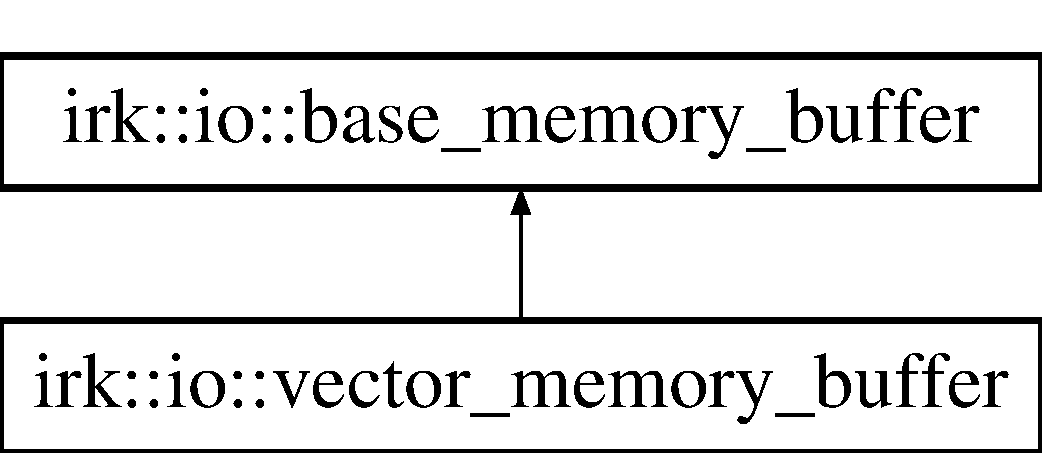
\includegraphics[height=2.000000cm]{classirk_1_1io_1_1vector__memory__buffer}
\end{center}
\end{figure}
\subsection*{Public Types}
\begin{DoxyCompactItemize}
\item 
using \mbox{\hyperlink{classirk_1_1io_1_1vector__memory__buffer_a3ad38262653ef0610f281f5a321c05de}{char\+\_\+type}} = char
\end{DoxyCompactItemize}
\subsection*{Public Member Functions}
\begin{DoxyCompactItemize}
\item 
virtual \mbox{\hyperlink{classirk_1_1io_1_1base__memory__buffer_a1b539180df4274dd4ad0402a0ac821ec}{char\+\_\+type}} $\ast$ \mbox{\hyperlink{classirk_1_1io_1_1vector__memory__buffer_a28ddafbb2610a463d13dc7fe5cf0708f}{data}} ()
\item 
virtual const \mbox{\hyperlink{classirk_1_1io_1_1base__memory__buffer_a1b539180df4274dd4ad0402a0ac821ec}{char\+\_\+type}} $\ast$ \mbox{\hyperlink{classirk_1_1io_1_1vector__memory__buffer_ad0d18022442c081ac51abb8da8b68e54}{data}} () const
\item 
virtual std\+::size\+\_\+t \mbox{\hyperlink{classirk_1_1io_1_1vector__memory__buffer_ab79eda0d916da980b78ecae09883bba1}{size}} () const
\end{DoxyCompactItemize}


\subsection{Member Typedef Documentation}
\mbox{\Hypertarget{classirk_1_1io_1_1vector__memory__buffer_a3ad38262653ef0610f281f5a321c05de}\label{classirk_1_1io_1_1vector__memory__buffer_a3ad38262653ef0610f281f5a321c05de}} 
\index{irk\+::io\+::vector\+\_\+memory\+\_\+buffer@{irk\+::io\+::vector\+\_\+memory\+\_\+buffer}!char\+\_\+type@{char\+\_\+type}}
\index{char\+\_\+type@{char\+\_\+type}!irk\+::io\+::vector\+\_\+memory\+\_\+buffer@{irk\+::io\+::vector\+\_\+memory\+\_\+buffer}}
\subsubsection{\texorpdfstring{char\+\_\+type}{char\_type}}
{\footnotesize\ttfamily using \mbox{\hyperlink{classirk_1_1io_1_1vector__memory__buffer_a3ad38262653ef0610f281f5a321c05de}{irk\+::io\+::vector\+\_\+memory\+\_\+buffer\+::char\+\_\+type}} =  char}



\subsection{Member Function Documentation}
\mbox{\Hypertarget{classirk_1_1io_1_1vector__memory__buffer_a28ddafbb2610a463d13dc7fe5cf0708f}\label{classirk_1_1io_1_1vector__memory__buffer_a28ddafbb2610a463d13dc7fe5cf0708f}} 
\index{irk\+::io\+::vector\+\_\+memory\+\_\+buffer@{irk\+::io\+::vector\+\_\+memory\+\_\+buffer}!data@{data}}
\index{data@{data}!irk\+::io\+::vector\+\_\+memory\+\_\+buffer@{irk\+::io\+::vector\+\_\+memory\+\_\+buffer}}
\subsubsection{\texorpdfstring{data()}{data()}\hspace{0.1cm}{\footnotesize\ttfamily [1/2]}}
{\footnotesize\ttfamily virtual \mbox{\hyperlink{classirk_1_1io_1_1base__memory__buffer_a1b539180df4274dd4ad0402a0ac821ec}{char\+\_\+type}}$\ast$ irk\+::io\+::vector\+\_\+memory\+\_\+buffer\+::data (\begin{DoxyParamCaption}{ }\end{DoxyParamCaption})\hspace{0.3cm}{\ttfamily [inline]}, {\ttfamily [virtual]}}



Implements \mbox{\hyperlink{classirk_1_1io_1_1base__memory__buffer_ae8247b83aae579cbc04b5432bd4858cc}{irk\+::io\+::base\+\_\+memory\+\_\+buffer}}.

\mbox{\Hypertarget{classirk_1_1io_1_1vector__memory__buffer_ad0d18022442c081ac51abb8da8b68e54}\label{classirk_1_1io_1_1vector__memory__buffer_ad0d18022442c081ac51abb8da8b68e54}} 
\index{irk\+::io\+::vector\+\_\+memory\+\_\+buffer@{irk\+::io\+::vector\+\_\+memory\+\_\+buffer}!data@{data}}
\index{data@{data}!irk\+::io\+::vector\+\_\+memory\+\_\+buffer@{irk\+::io\+::vector\+\_\+memory\+\_\+buffer}}
\subsubsection{\texorpdfstring{data()}{data()}\hspace{0.1cm}{\footnotesize\ttfamily [2/2]}}
{\footnotesize\ttfamily virtual const \mbox{\hyperlink{classirk_1_1io_1_1base__memory__buffer_a1b539180df4274dd4ad0402a0ac821ec}{char\+\_\+type}}$\ast$ irk\+::io\+::vector\+\_\+memory\+\_\+buffer\+::data (\begin{DoxyParamCaption}{ }\end{DoxyParamCaption}) const\hspace{0.3cm}{\ttfamily [inline]}, {\ttfamily [virtual]}}



Implements \mbox{\hyperlink{classirk_1_1io_1_1base__memory__buffer_a87bbff1a6d211e26f0c0aa924a980b9e}{irk\+::io\+::base\+\_\+memory\+\_\+buffer}}.

\mbox{\Hypertarget{classirk_1_1io_1_1vector__memory__buffer_ab79eda0d916da980b78ecae09883bba1}\label{classirk_1_1io_1_1vector__memory__buffer_ab79eda0d916da980b78ecae09883bba1}} 
\index{irk\+::io\+::vector\+\_\+memory\+\_\+buffer@{irk\+::io\+::vector\+\_\+memory\+\_\+buffer}!size@{size}}
\index{size@{size}!irk\+::io\+::vector\+\_\+memory\+\_\+buffer@{irk\+::io\+::vector\+\_\+memory\+\_\+buffer}}
\subsubsection{\texorpdfstring{size()}{size()}}
{\footnotesize\ttfamily virtual std\+::size\+\_\+t irk\+::io\+::vector\+\_\+memory\+\_\+buffer\+::size (\begin{DoxyParamCaption}{ }\end{DoxyParamCaption}) const\hspace{0.3cm}{\ttfamily [inline]}, {\ttfamily [virtual]}}



Implements \mbox{\hyperlink{classirk_1_1io_1_1base__memory__buffer_ae634ab934981e7e4baf5e1e67ef3b006}{irk\+::io\+::base\+\_\+memory\+\_\+buffer}}.



The documentation for this class was generated from the following file\+:\begin{DoxyCompactItemize}
\item 
include/irkit/io/\mbox{\hyperlink{memorybuffer_8hpp}{memorybuffer.\+hpp}}\end{DoxyCompactItemize}

\hypertarget{classirk_1_1vector__payload__list}{}\section{irk\+:\+:vector\+\_\+payload\+\_\+list$<$ PayloadT $>$ Class Template Reference}
\label{classirk_1_1vector__payload__list}\index{irk\+::vector\+\_\+payload\+\_\+list$<$ Payload\+T $>$@{irk\+::vector\+\_\+payload\+\_\+list$<$ Payload\+T $>$}}


{\ttfamily \#include $<$vector\+\_\+inverted\+\_\+list.\+hpp$>$}

\subsection*{Public Types}
\begin{DoxyCompactItemize}
\item 
using \mbox{\hyperlink{classirk_1_1vector__payload__list_a319d51342d589c056943998b362120ca}{size\+\_\+type}} = long
\item 
using \mbox{\hyperlink{classirk_1_1vector__payload__list_acded07bf18f4c147495e0b0dfdbf8922}{value\+\_\+type}} = PayloadT
\item 
using \mbox{\hyperlink{classirk_1_1vector__payload__list_a9312dea19fb0ee4e9c35e0def20e14d5}{self\+\_\+type}} = \mbox{\hyperlink{classirk_1_1vector__payload__list}{vector\+\_\+payload\+\_\+list}}$<$ PayloadT $>$
\item 
using \mbox{\hyperlink{classirk_1_1vector__payload__list_a33f425e324f556bba403c1700ff9915e}{iterator}} = \mbox{\hyperlink{classirk_1_1vector__block__iterator}{vector\+\_\+block\+\_\+iterator}}$<$ \mbox{\hyperlink{classirk_1_1vector__payload__list_a9312dea19fb0ee4e9c35e0def20e14d5}{self\+\_\+type}}, false $>$
\item 
using \mbox{\hyperlink{classirk_1_1vector__payload__list_abed614e4a2dad1f6ed890102297af020}{const\+\_\+iterator}} = \mbox{\hyperlink{classirk_1_1vector__payload__list_a33f425e324f556bba403c1700ff9915e}{iterator}}
\end{DoxyCompactItemize}
\subsection*{Public Member Functions}
\begin{DoxyCompactItemize}
\item 
\mbox{\hyperlink{classirk_1_1vector__payload__list_a3d56b520de4d0859f27c3be48fb8067c}{vector\+\_\+payload\+\_\+list}} (std\+::vector$<$ \mbox{\hyperlink{classirk_1_1vector__payload__list_acded07bf18f4c147495e0b0dfdbf8922}{value\+\_\+type}} $>$ vec)
\item 
\mbox{\hyperlink{classirk_1_1vector__payload__list_a319d51342d589c056943998b362120ca}{size\+\_\+type}} \mbox{\hyperlink{classirk_1_1vector__payload__list_ac3adf5af4d6301de780af1a1621a2084}{size}} () const
\item 
\mbox{\hyperlink{classirk_1_1vector__payload__list_a319d51342d589c056943998b362120ca}{size\+\_\+type}} \mbox{\hyperlink{classirk_1_1vector__payload__list_adb75734d3d14e43ff4eaf6fdac2125ff}{block\+\_\+size}} () const
\item 
void \mbox{\hyperlink{classirk_1_1vector__payload__list_a9924676b5747e4785acd933b77158864}{block\+\_\+size}} (\mbox{\hyperlink{classirk_1_1vector__payload__list_a319d51342d589c056943998b362120ca}{size\+\_\+type}} block\+\_\+size)
\item 
int \mbox{\hyperlink{classirk_1_1vector__payload__list_a7b28927adf91d29429f4089a3af41d19}{num\+\_\+blocks}} () const
\item 
const \mbox{\hyperlink{classirk_1_1vector__payload__list_acded07bf18f4c147495e0b0dfdbf8922}{value\+\_\+type}} \& \mbox{\hyperlink{classirk_1_1vector__payload__list_ae7225b27a6d4e7b3f14122c99497ebfa}{operator\mbox{[}$\,$\mbox{]}}} (std\+::size\+\_\+t pos) const
\item 
\mbox{\hyperlink{classirk_1_1vector__payload__list_a33f425e324f556bba403c1700ff9915e}{iterator}} \mbox{\hyperlink{classirk_1_1vector__payload__list_a35357c3fd3a0fb7b0308520b052844bf}{begin}} () const
\item 
\mbox{\hyperlink{classirk_1_1vector__payload__list_a33f425e324f556bba403c1700ff9915e}{iterator}} \mbox{\hyperlink{classirk_1_1vector__payload__list_ae8f6de3134a3fbb22ff3334363c1e583}{end}} () const
\item 
{\footnotesize template$<$class Document\+Iterator $>$ }\\\mbox{\hyperlink{classirk_1_1vector__payload__list_a33f425e324f556bba403c1700ff9915e}{iterator}} \mbox{\hyperlink{classirk_1_1vector__payload__list_a2490b25027ce0e8c2689557d06e910e8}{at}} (Document\+Iterator pos) const
\end{DoxyCompactItemize}


\subsection{Member Typedef Documentation}
\mbox{\Hypertarget{classirk_1_1vector__payload__list_abed614e4a2dad1f6ed890102297af020}\label{classirk_1_1vector__payload__list_abed614e4a2dad1f6ed890102297af020}} 
\index{irk\+::vector\+\_\+payload\+\_\+list@{irk\+::vector\+\_\+payload\+\_\+list}!const\+\_\+iterator@{const\+\_\+iterator}}
\index{const\+\_\+iterator@{const\+\_\+iterator}!irk\+::vector\+\_\+payload\+\_\+list@{irk\+::vector\+\_\+payload\+\_\+list}}
\subsubsection{\texorpdfstring{const\+\_\+iterator}{const\_iterator}}
{\footnotesize\ttfamily template$<$class PayloadT $>$ \\
using \mbox{\hyperlink{classirk_1_1vector__payload__list}{irk\+::vector\+\_\+payload\+\_\+list}}$<$ PayloadT $>$\+::\mbox{\hyperlink{classirk_1_1vector__payload__list_abed614e4a2dad1f6ed890102297af020}{const\+\_\+iterator}} =  \mbox{\hyperlink{classirk_1_1vector__payload__list_a33f425e324f556bba403c1700ff9915e}{iterator}}}

\mbox{\Hypertarget{classirk_1_1vector__payload__list_a33f425e324f556bba403c1700ff9915e}\label{classirk_1_1vector__payload__list_a33f425e324f556bba403c1700ff9915e}} 
\index{irk\+::vector\+\_\+payload\+\_\+list@{irk\+::vector\+\_\+payload\+\_\+list}!iterator@{iterator}}
\index{iterator@{iterator}!irk\+::vector\+\_\+payload\+\_\+list@{irk\+::vector\+\_\+payload\+\_\+list}}
\subsubsection{\texorpdfstring{iterator}{iterator}}
{\footnotesize\ttfamily template$<$class PayloadT $>$ \\
using \mbox{\hyperlink{classirk_1_1vector__payload__list}{irk\+::vector\+\_\+payload\+\_\+list}}$<$ PayloadT $>$\+::\mbox{\hyperlink{classirk_1_1vector__payload__list_a33f425e324f556bba403c1700ff9915e}{iterator}} =  \mbox{\hyperlink{classirk_1_1vector__block__iterator}{vector\+\_\+block\+\_\+iterator}}$<$\mbox{\hyperlink{classirk_1_1vector__payload__list_a9312dea19fb0ee4e9c35e0def20e14d5}{self\+\_\+type}}, false$>$}

\mbox{\Hypertarget{classirk_1_1vector__payload__list_a9312dea19fb0ee4e9c35e0def20e14d5}\label{classirk_1_1vector__payload__list_a9312dea19fb0ee4e9c35e0def20e14d5}} 
\index{irk\+::vector\+\_\+payload\+\_\+list@{irk\+::vector\+\_\+payload\+\_\+list}!self\+\_\+type@{self\+\_\+type}}
\index{self\+\_\+type@{self\+\_\+type}!irk\+::vector\+\_\+payload\+\_\+list@{irk\+::vector\+\_\+payload\+\_\+list}}
\subsubsection{\texorpdfstring{self\+\_\+type}{self\_type}}
{\footnotesize\ttfamily template$<$class PayloadT $>$ \\
using \mbox{\hyperlink{classirk_1_1vector__payload__list}{irk\+::vector\+\_\+payload\+\_\+list}}$<$ PayloadT $>$\+::\mbox{\hyperlink{classirk_1_1vector__payload__list_a9312dea19fb0ee4e9c35e0def20e14d5}{self\+\_\+type}} =  \mbox{\hyperlink{classirk_1_1vector__payload__list}{vector\+\_\+payload\+\_\+list}}$<$PayloadT$>$}

\mbox{\Hypertarget{classirk_1_1vector__payload__list_a319d51342d589c056943998b362120ca}\label{classirk_1_1vector__payload__list_a319d51342d589c056943998b362120ca}} 
\index{irk\+::vector\+\_\+payload\+\_\+list@{irk\+::vector\+\_\+payload\+\_\+list}!size\+\_\+type@{size\+\_\+type}}
\index{size\+\_\+type@{size\+\_\+type}!irk\+::vector\+\_\+payload\+\_\+list@{irk\+::vector\+\_\+payload\+\_\+list}}
\subsubsection{\texorpdfstring{size\+\_\+type}{size\_type}}
{\footnotesize\ttfamily template$<$class PayloadT $>$ \\
using \mbox{\hyperlink{classirk_1_1vector__payload__list}{irk\+::vector\+\_\+payload\+\_\+list}}$<$ PayloadT $>$\+::\mbox{\hyperlink{classirk_1_1vector__payload__list_a319d51342d589c056943998b362120ca}{size\+\_\+type}} =  long}

\mbox{\Hypertarget{classirk_1_1vector__payload__list_acded07bf18f4c147495e0b0dfdbf8922}\label{classirk_1_1vector__payload__list_acded07bf18f4c147495e0b0dfdbf8922}} 
\index{irk\+::vector\+\_\+payload\+\_\+list@{irk\+::vector\+\_\+payload\+\_\+list}!value\+\_\+type@{value\+\_\+type}}
\index{value\+\_\+type@{value\+\_\+type}!irk\+::vector\+\_\+payload\+\_\+list@{irk\+::vector\+\_\+payload\+\_\+list}}
\subsubsection{\texorpdfstring{value\+\_\+type}{value\_type}}
{\footnotesize\ttfamily template$<$class PayloadT $>$ \\
using \mbox{\hyperlink{classirk_1_1vector__payload__list}{irk\+::vector\+\_\+payload\+\_\+list}}$<$ PayloadT $>$\+::\mbox{\hyperlink{classirk_1_1vector__payload__list_acded07bf18f4c147495e0b0dfdbf8922}{value\+\_\+type}} =  PayloadT}



\subsection{Constructor \& Destructor Documentation}
\mbox{\Hypertarget{classirk_1_1vector__payload__list_a3d56b520de4d0859f27c3be48fb8067c}\label{classirk_1_1vector__payload__list_a3d56b520de4d0859f27c3be48fb8067c}} 
\index{irk\+::vector\+\_\+payload\+\_\+list@{irk\+::vector\+\_\+payload\+\_\+list}!vector\+\_\+payload\+\_\+list@{vector\+\_\+payload\+\_\+list}}
\index{vector\+\_\+payload\+\_\+list@{vector\+\_\+payload\+\_\+list}!irk\+::vector\+\_\+payload\+\_\+list@{irk\+::vector\+\_\+payload\+\_\+list}}
\subsubsection{\texorpdfstring{vector\+\_\+payload\+\_\+list()}{vector\_payload\_list()}}
{\footnotesize\ttfamily template$<$class PayloadT $>$ \\
\mbox{\hyperlink{classirk_1_1vector__payload__list}{irk\+::vector\+\_\+payload\+\_\+list}}$<$ PayloadT $>$\+::\mbox{\hyperlink{classirk_1_1vector__payload__list}{vector\+\_\+payload\+\_\+list}} (\begin{DoxyParamCaption}\item[{std\+::vector$<$ \mbox{\hyperlink{classirk_1_1vector__payload__list_acded07bf18f4c147495e0b0dfdbf8922}{value\+\_\+type}} $>$}]{vec }\end{DoxyParamCaption})\hspace{0.3cm}{\ttfamily [inline]}}



\subsection{Member Function Documentation}
\mbox{\Hypertarget{classirk_1_1vector__payload__list_a2490b25027ce0e8c2689557d06e910e8}\label{classirk_1_1vector__payload__list_a2490b25027ce0e8c2689557d06e910e8}} 
\index{irk\+::vector\+\_\+payload\+\_\+list@{irk\+::vector\+\_\+payload\+\_\+list}!at@{at}}
\index{at@{at}!irk\+::vector\+\_\+payload\+\_\+list@{irk\+::vector\+\_\+payload\+\_\+list}}
\subsubsection{\texorpdfstring{at()}{at()}}
{\footnotesize\ttfamily template$<$class PayloadT $>$ \\
template$<$class Document\+Iterator $>$ \\
\mbox{\hyperlink{classirk_1_1vector__payload__list_a33f425e324f556bba403c1700ff9915e}{iterator}} \mbox{\hyperlink{classirk_1_1vector__payload__list}{irk\+::vector\+\_\+payload\+\_\+list}}$<$ PayloadT $>$\+::at (\begin{DoxyParamCaption}\item[{Document\+Iterator}]{pos }\end{DoxyParamCaption}) const\hspace{0.3cm}{\ttfamily [inline]}}

\mbox{\Hypertarget{classirk_1_1vector__payload__list_a35357c3fd3a0fb7b0308520b052844bf}\label{classirk_1_1vector__payload__list_a35357c3fd3a0fb7b0308520b052844bf}} 
\index{irk\+::vector\+\_\+payload\+\_\+list@{irk\+::vector\+\_\+payload\+\_\+list}!begin@{begin}}
\index{begin@{begin}!irk\+::vector\+\_\+payload\+\_\+list@{irk\+::vector\+\_\+payload\+\_\+list}}
\subsubsection{\texorpdfstring{begin()}{begin()}}
{\footnotesize\ttfamily template$<$class PayloadT $>$ \\
\mbox{\hyperlink{classirk_1_1vector__payload__list_a33f425e324f556bba403c1700ff9915e}{iterator}} \mbox{\hyperlink{classirk_1_1vector__payload__list}{irk\+::vector\+\_\+payload\+\_\+list}}$<$ PayloadT $>$\+::begin (\begin{DoxyParamCaption}{ }\end{DoxyParamCaption}) const\hspace{0.3cm}{\ttfamily [inline]}}

\mbox{\Hypertarget{classirk_1_1vector__payload__list_adb75734d3d14e43ff4eaf6fdac2125ff}\label{classirk_1_1vector__payload__list_adb75734d3d14e43ff4eaf6fdac2125ff}} 
\index{irk\+::vector\+\_\+payload\+\_\+list@{irk\+::vector\+\_\+payload\+\_\+list}!block\+\_\+size@{block\+\_\+size}}
\index{block\+\_\+size@{block\+\_\+size}!irk\+::vector\+\_\+payload\+\_\+list@{irk\+::vector\+\_\+payload\+\_\+list}}
\subsubsection{\texorpdfstring{block\+\_\+size()}{block\_size()}\hspace{0.1cm}{\footnotesize\ttfamily [1/2]}}
{\footnotesize\ttfamily template$<$class PayloadT $>$ \\
\mbox{\hyperlink{classirk_1_1vector__payload__list_a319d51342d589c056943998b362120ca}{size\+\_\+type}} \mbox{\hyperlink{classirk_1_1vector__payload__list}{irk\+::vector\+\_\+payload\+\_\+list}}$<$ PayloadT $>$\+::block\+\_\+size (\begin{DoxyParamCaption}{ }\end{DoxyParamCaption}) const\hspace{0.3cm}{\ttfamily [inline]}}

\mbox{\Hypertarget{classirk_1_1vector__payload__list_a9924676b5747e4785acd933b77158864}\label{classirk_1_1vector__payload__list_a9924676b5747e4785acd933b77158864}} 
\index{irk\+::vector\+\_\+payload\+\_\+list@{irk\+::vector\+\_\+payload\+\_\+list}!block\+\_\+size@{block\+\_\+size}}
\index{block\+\_\+size@{block\+\_\+size}!irk\+::vector\+\_\+payload\+\_\+list@{irk\+::vector\+\_\+payload\+\_\+list}}
\subsubsection{\texorpdfstring{block\+\_\+size()}{block\_size()}\hspace{0.1cm}{\footnotesize\ttfamily [2/2]}}
{\footnotesize\ttfamily template$<$class PayloadT $>$ \\
void \mbox{\hyperlink{classirk_1_1vector__payload__list}{irk\+::vector\+\_\+payload\+\_\+list}}$<$ PayloadT $>$\+::block\+\_\+size (\begin{DoxyParamCaption}\item[{\mbox{\hyperlink{classirk_1_1vector__payload__list_a319d51342d589c056943998b362120ca}{size\+\_\+type}}}]{block\+\_\+size }\end{DoxyParamCaption})\hspace{0.3cm}{\ttfamily [inline]}}

\mbox{\Hypertarget{classirk_1_1vector__payload__list_ae8f6de3134a3fbb22ff3334363c1e583}\label{classirk_1_1vector__payload__list_ae8f6de3134a3fbb22ff3334363c1e583}} 
\index{irk\+::vector\+\_\+payload\+\_\+list@{irk\+::vector\+\_\+payload\+\_\+list}!end@{end}}
\index{end@{end}!irk\+::vector\+\_\+payload\+\_\+list@{irk\+::vector\+\_\+payload\+\_\+list}}
\subsubsection{\texorpdfstring{end()}{end()}}
{\footnotesize\ttfamily template$<$class PayloadT $>$ \\
\mbox{\hyperlink{classirk_1_1vector__payload__list_a33f425e324f556bba403c1700ff9915e}{iterator}} \mbox{\hyperlink{classirk_1_1vector__payload__list}{irk\+::vector\+\_\+payload\+\_\+list}}$<$ PayloadT $>$\+::end (\begin{DoxyParamCaption}{ }\end{DoxyParamCaption}) const\hspace{0.3cm}{\ttfamily [inline]}}

\mbox{\Hypertarget{classirk_1_1vector__payload__list_a7b28927adf91d29429f4089a3af41d19}\label{classirk_1_1vector__payload__list_a7b28927adf91d29429f4089a3af41d19}} 
\index{irk\+::vector\+\_\+payload\+\_\+list@{irk\+::vector\+\_\+payload\+\_\+list}!num\+\_\+blocks@{num\+\_\+blocks}}
\index{num\+\_\+blocks@{num\+\_\+blocks}!irk\+::vector\+\_\+payload\+\_\+list@{irk\+::vector\+\_\+payload\+\_\+list}}
\subsubsection{\texorpdfstring{num\+\_\+blocks()}{num\_blocks()}}
{\footnotesize\ttfamily template$<$class PayloadT $>$ \\
int \mbox{\hyperlink{classirk_1_1vector__payload__list}{irk\+::vector\+\_\+payload\+\_\+list}}$<$ PayloadT $>$\+::num\+\_\+blocks (\begin{DoxyParamCaption}{ }\end{DoxyParamCaption}) const\hspace{0.3cm}{\ttfamily [inline]}}

\mbox{\Hypertarget{classirk_1_1vector__payload__list_ae7225b27a6d4e7b3f14122c99497ebfa}\label{classirk_1_1vector__payload__list_ae7225b27a6d4e7b3f14122c99497ebfa}} 
\index{irk\+::vector\+\_\+payload\+\_\+list@{irk\+::vector\+\_\+payload\+\_\+list}!operator\mbox{[}\mbox{]}@{operator[]}}
\index{operator\mbox{[}\mbox{]}@{operator[]}!irk\+::vector\+\_\+payload\+\_\+list@{irk\+::vector\+\_\+payload\+\_\+list}}
\subsubsection{\texorpdfstring{operator[]()}{operator[]()}}
{\footnotesize\ttfamily template$<$class PayloadT $>$ \\
const \mbox{\hyperlink{classirk_1_1vector__payload__list_acded07bf18f4c147495e0b0dfdbf8922}{value\+\_\+type}}\& \mbox{\hyperlink{classirk_1_1vector__payload__list}{irk\+::vector\+\_\+payload\+\_\+list}}$<$ PayloadT $>$\+::operator\mbox{[}$\,$\mbox{]} (\begin{DoxyParamCaption}\item[{std\+::size\+\_\+t}]{pos }\end{DoxyParamCaption}) const\hspace{0.3cm}{\ttfamily [inline]}}

\mbox{\Hypertarget{classirk_1_1vector__payload__list_ac3adf5af4d6301de780af1a1621a2084}\label{classirk_1_1vector__payload__list_ac3adf5af4d6301de780af1a1621a2084}} 
\index{irk\+::vector\+\_\+payload\+\_\+list@{irk\+::vector\+\_\+payload\+\_\+list}!size@{size}}
\index{size@{size}!irk\+::vector\+\_\+payload\+\_\+list@{irk\+::vector\+\_\+payload\+\_\+list}}
\subsubsection{\texorpdfstring{size()}{size()}}
{\footnotesize\ttfamily template$<$class PayloadT $>$ \\
\mbox{\hyperlink{classirk_1_1vector__payload__list_a319d51342d589c056943998b362120ca}{size\+\_\+type}} \mbox{\hyperlink{classirk_1_1vector__payload__list}{irk\+::vector\+\_\+payload\+\_\+list}}$<$ PayloadT $>$\+::size (\begin{DoxyParamCaption}{ }\end{DoxyParamCaption}) const\hspace{0.3cm}{\ttfamily [inline]}}



The documentation for this class was generated from the following file\+:\begin{DoxyCompactItemize}
\item 
include/irkit/index/\mbox{\hyperlink{vector__inverted__list_8hpp}{vector\+\_\+inverted\+\_\+list.\+hpp}}\end{DoxyCompactItemize}

\hypertarget{classirkit_1_1io_1_1warc__format__exception}{}\section{irkit\+:\+:io\+:\+:warc\+\_\+format\+\_\+exception Class Reference}
\label{classirkit_1_1io_1_1warc__format__exception}\index{irkit\+::io\+::warc\+\_\+format\+\_\+exception@{irkit\+::io\+::warc\+\_\+format\+\_\+exception}}


Represents an error during parsing W\+A\+RC format.  




{\ttfamily \#include $<$warc.\+hpp$>$}

Inheritance diagram for irkit\+:\+:io\+:\+:warc\+\_\+format\+\_\+exception\+:\begin{figure}[H]
\begin{center}
\leavevmode
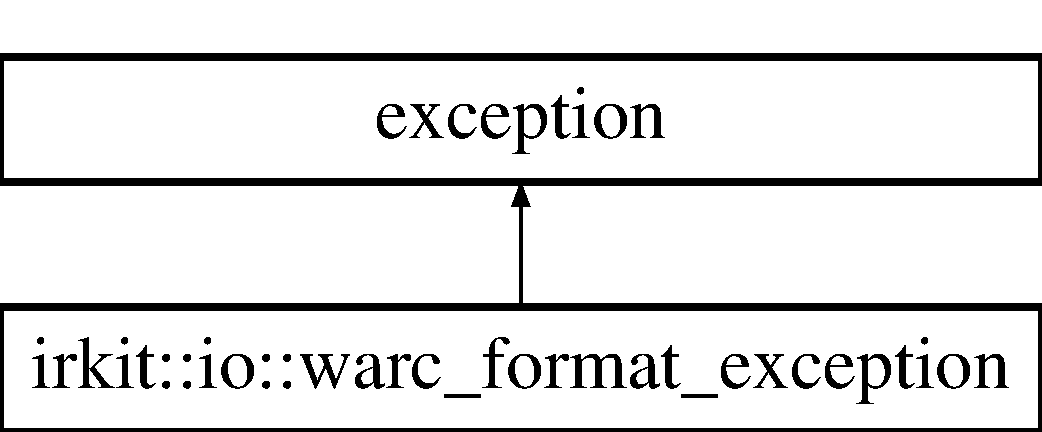
\includegraphics[height=2.000000cm]{classirkit_1_1io_1_1warc__format__exception}
\end{center}
\end{figure}
\subsection*{Public Member Functions}
\begin{DoxyCompactItemize}
\item 
\mbox{\hyperlink{classirkit_1_1io_1_1warc__format__exception_a2c328f2114bf1bba82e8a1b88b3bd6ce}{warc\+\_\+format\+\_\+exception}} (std\+::string \mbox{\hyperlink{classirkit_1_1io_1_1warc__format__exception_abf4c3f70a23e8b7b602db1ffa2c3b416}{line}}, std\+::string message)
\item 
const char $\ast$ \mbox{\hyperlink{classirkit_1_1io_1_1warc__format__exception_a2571f83ce38f5b6765e008fd643f38c5}{what}} () const  throw ()
\item 
const std\+::string \& \mbox{\hyperlink{classirkit_1_1io_1_1warc__format__exception_abf4c3f70a23e8b7b602db1ffa2c3b416}{line}} () const
\end{DoxyCompactItemize}


\subsection{Detailed Description}
Represents an error during parsing W\+A\+RC format. 

\subsection{Constructor \& Destructor Documentation}
\mbox{\Hypertarget{classirkit_1_1io_1_1warc__format__exception_a2c328f2114bf1bba82e8a1b88b3bd6ce}\label{classirkit_1_1io_1_1warc__format__exception_a2c328f2114bf1bba82e8a1b88b3bd6ce}} 
\index{irkit\+::io\+::warc\+\_\+format\+\_\+exception@{irkit\+::io\+::warc\+\_\+format\+\_\+exception}!warc\+\_\+format\+\_\+exception@{warc\+\_\+format\+\_\+exception}}
\index{warc\+\_\+format\+\_\+exception@{warc\+\_\+format\+\_\+exception}!irkit\+::io\+::warc\+\_\+format\+\_\+exception@{irkit\+::io\+::warc\+\_\+format\+\_\+exception}}
\subsubsection{\texorpdfstring{warc\+\_\+format\+\_\+exception()}{warc\_format\_exception()}}
{\footnotesize\ttfamily irkit\+::io\+::warc\+\_\+format\+\_\+exception\+::warc\+\_\+format\+\_\+exception (\begin{DoxyParamCaption}\item[{std\+::string}]{line,  }\item[{std\+::string}]{message }\end{DoxyParamCaption})\hspace{0.3cm}{\ttfamily [inline]}}



\subsection{Member Function Documentation}
\mbox{\Hypertarget{classirkit_1_1io_1_1warc__format__exception_abf4c3f70a23e8b7b602db1ffa2c3b416}\label{classirkit_1_1io_1_1warc__format__exception_abf4c3f70a23e8b7b602db1ffa2c3b416}} 
\index{irkit\+::io\+::warc\+\_\+format\+\_\+exception@{irkit\+::io\+::warc\+\_\+format\+\_\+exception}!line@{line}}
\index{line@{line}!irkit\+::io\+::warc\+\_\+format\+\_\+exception@{irkit\+::io\+::warc\+\_\+format\+\_\+exception}}
\subsubsection{\texorpdfstring{line()}{line()}}
{\footnotesize\ttfamily const std\+::string\& irkit\+::io\+::warc\+\_\+format\+\_\+exception\+::line (\begin{DoxyParamCaption}{ }\end{DoxyParamCaption}) const\hspace{0.3cm}{\ttfamily [inline]}}

\mbox{\Hypertarget{classirkit_1_1io_1_1warc__format__exception_a2571f83ce38f5b6765e008fd643f38c5}\label{classirkit_1_1io_1_1warc__format__exception_a2571f83ce38f5b6765e008fd643f38c5}} 
\index{irkit\+::io\+::warc\+\_\+format\+\_\+exception@{irkit\+::io\+::warc\+\_\+format\+\_\+exception}!what@{what}}
\index{what@{what}!irkit\+::io\+::warc\+\_\+format\+\_\+exception@{irkit\+::io\+::warc\+\_\+format\+\_\+exception}}
\subsubsection{\texorpdfstring{what()}{what()}}
{\footnotesize\ttfamily const char$\ast$ irkit\+::io\+::warc\+\_\+format\+\_\+exception\+::what (\begin{DoxyParamCaption}{ }\end{DoxyParamCaption}) const throw  ) \hspace{0.3cm}{\ttfamily [inline]}}



The documentation for this class was generated from the following file\+:\begin{DoxyCompactItemize}
\item 
include/irkit/io/\mbox{\hyperlink{warc_8hpp}{warc.\+hpp}}\end{DoxyCompactItemize}

\hypertarget{classirkit_1_1io_1_1warc__record}{}\section{irkit\+:\+:io\+:\+:warc\+\_\+record Class Reference}
\label{classirkit_1_1io_1_1warc__record}\index{irkit\+::io\+::warc\+\_\+record@{irkit\+::io\+::warc\+\_\+record}}


A W\+A\+RC record.  




{\ttfamily \#include $<$warc.\+hpp$>$}

\subsection*{Public Member Functions}
\begin{DoxyCompactItemize}
\item 
\mbox{\hyperlink{classirkit_1_1io_1_1warc__record_adbf4f3980cefeb456de898d0415b4e36}{warc\+\_\+record}} ()=default
\item 
\mbox{\hyperlink{classirkit_1_1io_1_1warc__record_a88b5dab62123bbbef9cd5b58b74e76e7}{warc\+\_\+record}} (std\+::string version)
\item 
std\+::string \mbox{\hyperlink{classirkit_1_1io_1_1warc__record_a2d8b476a009344abc9f1d41f5c9e3de0}{type}} () const
\item 
std\+::string \mbox{\hyperlink{classirkit_1_1io_1_1warc__record_a46c46772b6e77545047ab9c8cbe5d281}{content\+\_\+length}} () const
\item 
std\+::string \& \mbox{\hyperlink{classirkit_1_1io_1_1warc__record_ab53f61c5eb11564671280cdd7666352b}{content}} ()
\item 
const std\+::string \& \mbox{\hyperlink{classirkit_1_1io_1_1warc__record_a3ac994f3690d28a5add45485a3b388ec}{content}} () const
\item 
std\+::string \mbox{\hyperlink{classirkit_1_1io_1_1warc__record_ae5bab7d203ec2705e3ae9c4d20b1286c}{url}} () const
\item 
std\+::string \mbox{\hyperlink{classirkit_1_1io_1_1warc__record_a5a0ce07bbe522fedf5a49d4cac2c1520}{trecid}} () const
\end{DoxyCompactItemize}
\subsection*{Friends}
\begin{DoxyCompactItemize}
\item 
std\+::istream \& \mbox{\hyperlink{classirkit_1_1io_1_1warc__record_a3ffe8b4b7fc8c809d6ce483d2272f7a3}{read\+\_\+warc\+\_\+record}} (std\+::istream \&in, \mbox{\hyperlink{classirkit_1_1io_1_1warc__record}{warc\+\_\+record}} \&record)
\begin{DoxyCompactList}\small\item\em Read a W\+A\+RC record from an input stream. \end{DoxyCompactList}\end{DoxyCompactItemize}


\subsection{Detailed Description}
A W\+A\+RC record. 

\subsection{Constructor \& Destructor Documentation}
\mbox{\Hypertarget{classirkit_1_1io_1_1warc__record_adbf4f3980cefeb456de898d0415b4e36}\label{classirkit_1_1io_1_1warc__record_adbf4f3980cefeb456de898d0415b4e36}} 
\index{irkit\+::io\+::warc\+\_\+record@{irkit\+::io\+::warc\+\_\+record}!warc\+\_\+record@{warc\+\_\+record}}
\index{warc\+\_\+record@{warc\+\_\+record}!irkit\+::io\+::warc\+\_\+record@{irkit\+::io\+::warc\+\_\+record}}
\subsubsection{\texorpdfstring{warc\+\_\+record()}{warc\_record()}\hspace{0.1cm}{\footnotesize\ttfamily [1/2]}}
{\footnotesize\ttfamily irkit\+::io\+::warc\+\_\+record\+::warc\+\_\+record (\begin{DoxyParamCaption}{ }\end{DoxyParamCaption})\hspace{0.3cm}{\ttfamily [default]}}

\mbox{\Hypertarget{classirkit_1_1io_1_1warc__record_a88b5dab62123bbbef9cd5b58b74e76e7}\label{classirkit_1_1io_1_1warc__record_a88b5dab62123bbbef9cd5b58b74e76e7}} 
\index{irkit\+::io\+::warc\+\_\+record@{irkit\+::io\+::warc\+\_\+record}!warc\+\_\+record@{warc\+\_\+record}}
\index{warc\+\_\+record@{warc\+\_\+record}!irkit\+::io\+::warc\+\_\+record@{irkit\+::io\+::warc\+\_\+record}}
\subsubsection{\texorpdfstring{warc\+\_\+record()}{warc\_record()}\hspace{0.1cm}{\footnotesize\ttfamily [2/2]}}
{\footnotesize\ttfamily irkit\+::io\+::warc\+\_\+record\+::warc\+\_\+record (\begin{DoxyParamCaption}\item[{std\+::string}]{version }\end{DoxyParamCaption})\hspace{0.3cm}{\ttfamily [inline]}}



\subsection{Member Function Documentation}
\mbox{\Hypertarget{classirkit_1_1io_1_1warc__record_ab53f61c5eb11564671280cdd7666352b}\label{classirkit_1_1io_1_1warc__record_ab53f61c5eb11564671280cdd7666352b}} 
\index{irkit\+::io\+::warc\+\_\+record@{irkit\+::io\+::warc\+\_\+record}!content@{content}}
\index{content@{content}!irkit\+::io\+::warc\+\_\+record@{irkit\+::io\+::warc\+\_\+record}}
\subsubsection{\texorpdfstring{content()}{content()}\hspace{0.1cm}{\footnotesize\ttfamily [1/2]}}
{\footnotesize\ttfamily std\+::string\& irkit\+::io\+::warc\+\_\+record\+::content (\begin{DoxyParamCaption}{ }\end{DoxyParamCaption})\hspace{0.3cm}{\ttfamily [inline]}}

\mbox{\Hypertarget{classirkit_1_1io_1_1warc__record_a3ac994f3690d28a5add45485a3b388ec}\label{classirkit_1_1io_1_1warc__record_a3ac994f3690d28a5add45485a3b388ec}} 
\index{irkit\+::io\+::warc\+\_\+record@{irkit\+::io\+::warc\+\_\+record}!content@{content}}
\index{content@{content}!irkit\+::io\+::warc\+\_\+record@{irkit\+::io\+::warc\+\_\+record}}
\subsubsection{\texorpdfstring{content()}{content()}\hspace{0.1cm}{\footnotesize\ttfamily [2/2]}}
{\footnotesize\ttfamily const std\+::string\& irkit\+::io\+::warc\+\_\+record\+::content (\begin{DoxyParamCaption}{ }\end{DoxyParamCaption}) const\hspace{0.3cm}{\ttfamily [inline]}}

\mbox{\Hypertarget{classirkit_1_1io_1_1warc__record_a46c46772b6e77545047ab9c8cbe5d281}\label{classirkit_1_1io_1_1warc__record_a46c46772b6e77545047ab9c8cbe5d281}} 
\index{irkit\+::io\+::warc\+\_\+record@{irkit\+::io\+::warc\+\_\+record}!content\+\_\+length@{content\+\_\+length}}
\index{content\+\_\+length@{content\+\_\+length}!irkit\+::io\+::warc\+\_\+record@{irkit\+::io\+::warc\+\_\+record}}
\subsubsection{\texorpdfstring{content\+\_\+length()}{content\_length()}}
{\footnotesize\ttfamily std\+::string irkit\+::io\+::warc\+\_\+record\+::content\+\_\+length (\begin{DoxyParamCaption}{ }\end{DoxyParamCaption}) const\hspace{0.3cm}{\ttfamily [inline]}}

\mbox{\Hypertarget{classirkit_1_1io_1_1warc__record_a5a0ce07bbe522fedf5a49d4cac2c1520}\label{classirkit_1_1io_1_1warc__record_a5a0ce07bbe522fedf5a49d4cac2c1520}} 
\index{irkit\+::io\+::warc\+\_\+record@{irkit\+::io\+::warc\+\_\+record}!trecid@{trecid}}
\index{trecid@{trecid}!irkit\+::io\+::warc\+\_\+record@{irkit\+::io\+::warc\+\_\+record}}
\subsubsection{\texorpdfstring{trecid()}{trecid()}}
{\footnotesize\ttfamily std\+::string irkit\+::io\+::warc\+\_\+record\+::trecid (\begin{DoxyParamCaption}{ }\end{DoxyParamCaption}) const\hspace{0.3cm}{\ttfamily [inline]}}

\mbox{\Hypertarget{classirkit_1_1io_1_1warc__record_a2d8b476a009344abc9f1d41f5c9e3de0}\label{classirkit_1_1io_1_1warc__record_a2d8b476a009344abc9f1d41f5c9e3de0}} 
\index{irkit\+::io\+::warc\+\_\+record@{irkit\+::io\+::warc\+\_\+record}!type@{type}}
\index{type@{type}!irkit\+::io\+::warc\+\_\+record@{irkit\+::io\+::warc\+\_\+record}}
\subsubsection{\texorpdfstring{type()}{type()}}
{\footnotesize\ttfamily std\+::string irkit\+::io\+::warc\+\_\+record\+::type (\begin{DoxyParamCaption}{ }\end{DoxyParamCaption}) const\hspace{0.3cm}{\ttfamily [inline]}}

\mbox{\Hypertarget{classirkit_1_1io_1_1warc__record_ae5bab7d203ec2705e3ae9c4d20b1286c}\label{classirkit_1_1io_1_1warc__record_ae5bab7d203ec2705e3ae9c4d20b1286c}} 
\index{irkit\+::io\+::warc\+\_\+record@{irkit\+::io\+::warc\+\_\+record}!url@{url}}
\index{url@{url}!irkit\+::io\+::warc\+\_\+record@{irkit\+::io\+::warc\+\_\+record}}
\subsubsection{\texorpdfstring{url()}{url()}}
{\footnotesize\ttfamily std\+::string irkit\+::io\+::warc\+\_\+record\+::url (\begin{DoxyParamCaption}{ }\end{DoxyParamCaption}) const\hspace{0.3cm}{\ttfamily [inline]}}



\subsection{Friends And Related Function Documentation}
\mbox{\Hypertarget{classirkit_1_1io_1_1warc__record_a3ffe8b4b7fc8c809d6ce483d2272f7a3}\label{classirkit_1_1io_1_1warc__record_a3ffe8b4b7fc8c809d6ce483d2272f7a3}} 
\index{irkit\+::io\+::warc\+\_\+record@{irkit\+::io\+::warc\+\_\+record}!read\+\_\+warc\+\_\+record@{read\+\_\+warc\+\_\+record}}
\index{read\+\_\+warc\+\_\+record@{read\+\_\+warc\+\_\+record}!irkit\+::io\+::warc\+\_\+record@{irkit\+::io\+::warc\+\_\+record}}
\subsubsection{\texorpdfstring{read\+\_\+warc\+\_\+record}{read\_warc\_record}}
{\footnotesize\ttfamily std\+::istream\& read\+\_\+warc\+\_\+record (\begin{DoxyParamCaption}\item[{std\+::istream \&}]{in,  }\item[{\mbox{\hyperlink{classirkit_1_1io_1_1warc__record}{warc\+\_\+record}} \&}]{record }\end{DoxyParamCaption})\hspace{0.3cm}{\ttfamily [friend]}}



Read a W\+A\+RC record from an input stream. 


\begin{DoxyParams}{Parameters}
{\em in} & an input stream \\
\hline
{\em record} & a W\+A\+RC record reference to write to \\
\hline
\end{DoxyParams}
\begin{DoxyReturn}{Returns}
{\ttfamily in} stream 
\end{DoxyReturn}


The documentation for this class was generated from the following file\+:\begin{DoxyCompactItemize}
\item 
include/irkit/io/\mbox{\hyperlink{warc_8hpp}{warc.\+hpp}}\end{DoxyCompactItemize}

\hypertarget{structirk_1_1index_1_1write__fn}{}\section{irk\+:\+:index\+:\+:write\+\_\+fn$<$ T $>$ Struct Template Reference}
\label{structirk_1_1index_1_1write__fn}\index{irk\+::index\+::write\+\_\+fn$<$ T $>$@{irk\+::index\+::write\+\_\+fn$<$ T $>$}}


{\ttfamily \#include $<$skiplist.\+hpp$>$}

\subsection*{Public Member Functions}
\begin{DoxyCompactItemize}
\item 
std\+::ostream \& \mbox{\hyperlink{structirk_1_1index_1_1write__fn_a66bc60aa84f1256fad609bd056b5d68d}{operator()}} (std\+::ostream \&out, T value) const
\end{DoxyCompactItemize}


\subsection{Member Function Documentation}
\mbox{\Hypertarget{structirk_1_1index_1_1write__fn_a66bc60aa84f1256fad609bd056b5d68d}\label{structirk_1_1index_1_1write__fn_a66bc60aa84f1256fad609bd056b5d68d}} 
\index{irk\+::index\+::write\+\_\+fn@{irk\+::index\+::write\+\_\+fn}!operator()@{operator()}}
\index{operator()@{operator()}!irk\+::index\+::write\+\_\+fn@{irk\+::index\+::write\+\_\+fn}}
\subsubsection{\texorpdfstring{operator()()}{operator()()}}
{\footnotesize\ttfamily template$<$class T $>$ \\
std\+::ostream\& \mbox{\hyperlink{structirk_1_1index_1_1write__fn}{irk\+::index\+::write\+\_\+fn}}$<$ T $>$\+::operator() (\begin{DoxyParamCaption}\item[{std\+::ostream \&}]{out,  }\item[{T}]{value }\end{DoxyParamCaption}) const\hspace{0.3cm}{\ttfamily [inline]}}



The documentation for this struct was generated from the following file\+:\begin{DoxyCompactItemize}
\item 
include/irkit/index/\mbox{\hyperlink{skiplist_8hpp}{skiplist.\+hpp}}\end{DoxyCompactItemize}

\hypertarget{classirk_1_1index_1_1zipped__payload__list__view}{}\section{irk\+:\+:index\+:\+:zipped\+\_\+payload\+\_\+list\+\_\+view$<$ Payload $>$ Class Template Reference}
\label{classirk_1_1index_1_1zipped__payload__list__view}\index{irk\+::index\+::zipped\+\_\+payload\+\_\+list\+\_\+view$<$ Payload $>$@{irk\+::index\+::zipped\+\_\+payload\+\_\+list\+\_\+view$<$ Payload $>$}}


{\ttfamily \#include $<$block\+\_\+inverted\+\_\+list.\+hpp$>$}

\subsection*{Classes}
\begin{DoxyCompactItemize}
\item 
class \mbox{\hyperlink{classirk_1_1index_1_1zipped__payload__list__view_1_1iterator}{iterator}}
\end{DoxyCompactItemize}
\subsection*{Public Types}
\begin{DoxyCompactItemize}
\item 
using \mbox{\hyperlink{classirk_1_1index_1_1zipped__payload__list__view_a5dae0163f955f3e253686927c3bd750c}{value\+\_\+type}} = std\+::tuple$<$ Payload... $>$
\item 
using \mbox{\hyperlink{classirk_1_1index_1_1zipped__payload__list__view_a63e493d2777f8c4667625cbfbfcc75f1}{reference}} = \mbox{\hyperlink{classirk_1_1index_1_1zipped__payload__list__view_a5dae0163f955f3e253686927c3bd750c}{value\+\_\+type}}
\item 
using \mbox{\hyperlink{classirk_1_1index_1_1zipped__payload__list__view_ac64dd5a88b49bb118bb780083f62907d}{difference\+\_\+type}} = long
\end{DoxyCompactItemize}
\subsection*{Public Member Functions}
\begin{DoxyCompactItemize}
\item 
\mbox{\hyperlink{classirk_1_1index_1_1zipped__payload__list__view_ac1f66a414d5196e98ce325d1684bee36}{zipped\+\_\+payload\+\_\+list\+\_\+view}} ()=default
\item 
\mbox{\hyperlink{classirk_1_1index_1_1zipped__payload__list__view_a47c5a4bf0f8fd1baf10f50bba6325092}{zipped\+\_\+payload\+\_\+list\+\_\+view}} (\mbox{\hyperlink{classirk_1_1index_1_1block__payload__list__view}{block\+\_\+payload\+\_\+list\+\_\+view}}$<$ Payload $>$... views)
\item 
\mbox{\hyperlink{classirk_1_1index_1_1zipped__payload__list__view_1_1iterator}{iterator}} \mbox{\hyperlink{classirk_1_1index_1_1zipped__payload__list__view_aec7df8626683a4f71aa2b733d36d0a4c}{begin}} () const
\item 
\mbox{\hyperlink{classirk_1_1index_1_1zipped__payload__list__view_1_1iterator}{iterator}} \mbox{\hyperlink{classirk_1_1index_1_1zipped__payload__list__view_af10848c654db6e4d0b342fe764c0f77b}{end}} () const
\end{DoxyCompactItemize}


\subsection{Member Typedef Documentation}
\mbox{\Hypertarget{classirk_1_1index_1_1zipped__payload__list__view_ac64dd5a88b49bb118bb780083f62907d}\label{classirk_1_1index_1_1zipped__payload__list__view_ac64dd5a88b49bb118bb780083f62907d}} 
\index{irk\+::index\+::zipped\+\_\+payload\+\_\+list\+\_\+view@{irk\+::index\+::zipped\+\_\+payload\+\_\+list\+\_\+view}!difference\+\_\+type@{difference\+\_\+type}}
\index{difference\+\_\+type@{difference\+\_\+type}!irk\+::index\+::zipped\+\_\+payload\+\_\+list\+\_\+view@{irk\+::index\+::zipped\+\_\+payload\+\_\+list\+\_\+view}}
\subsubsection{\texorpdfstring{difference\+\_\+type}{difference\_type}}
{\footnotesize\ttfamily template$<$class ... Payload$>$ \\
using \mbox{\hyperlink{classirk_1_1index_1_1zipped__payload__list__view}{irk\+::index\+::zipped\+\_\+payload\+\_\+list\+\_\+view}}$<$ Payload $>$\+::\mbox{\hyperlink{classirk_1_1index_1_1zipped__payload__list__view_ac64dd5a88b49bb118bb780083f62907d}{difference\+\_\+type}} =  long}

\mbox{\Hypertarget{classirk_1_1index_1_1zipped__payload__list__view_a63e493d2777f8c4667625cbfbfcc75f1}\label{classirk_1_1index_1_1zipped__payload__list__view_a63e493d2777f8c4667625cbfbfcc75f1}} 
\index{irk\+::index\+::zipped\+\_\+payload\+\_\+list\+\_\+view@{irk\+::index\+::zipped\+\_\+payload\+\_\+list\+\_\+view}!reference@{reference}}
\index{reference@{reference}!irk\+::index\+::zipped\+\_\+payload\+\_\+list\+\_\+view@{irk\+::index\+::zipped\+\_\+payload\+\_\+list\+\_\+view}}
\subsubsection{\texorpdfstring{reference}{reference}}
{\footnotesize\ttfamily template$<$class ... Payload$>$ \\
using \mbox{\hyperlink{classirk_1_1index_1_1zipped__payload__list__view}{irk\+::index\+::zipped\+\_\+payload\+\_\+list\+\_\+view}}$<$ Payload $>$\+::\mbox{\hyperlink{classirk_1_1index_1_1zipped__payload__list__view_a63e493d2777f8c4667625cbfbfcc75f1}{reference}} =  \mbox{\hyperlink{classirk_1_1index_1_1zipped__payload__list__view_a5dae0163f955f3e253686927c3bd750c}{value\+\_\+type}}}

\mbox{\Hypertarget{classirk_1_1index_1_1zipped__payload__list__view_a5dae0163f955f3e253686927c3bd750c}\label{classirk_1_1index_1_1zipped__payload__list__view_a5dae0163f955f3e253686927c3bd750c}} 
\index{irk\+::index\+::zipped\+\_\+payload\+\_\+list\+\_\+view@{irk\+::index\+::zipped\+\_\+payload\+\_\+list\+\_\+view}!value\+\_\+type@{value\+\_\+type}}
\index{value\+\_\+type@{value\+\_\+type}!irk\+::index\+::zipped\+\_\+payload\+\_\+list\+\_\+view@{irk\+::index\+::zipped\+\_\+payload\+\_\+list\+\_\+view}}
\subsubsection{\texorpdfstring{value\+\_\+type}{value\_type}}
{\footnotesize\ttfamily template$<$class ... Payload$>$ \\
using \mbox{\hyperlink{classirk_1_1index_1_1zipped__payload__list__view}{irk\+::index\+::zipped\+\_\+payload\+\_\+list\+\_\+view}}$<$ Payload $>$\+::\mbox{\hyperlink{classirk_1_1index_1_1zipped__payload__list__view_a5dae0163f955f3e253686927c3bd750c}{value\+\_\+type}} =  std\+::tuple$<$Payload...$>$}



\subsection{Constructor \& Destructor Documentation}
\mbox{\Hypertarget{classirk_1_1index_1_1zipped__payload__list__view_ac1f66a414d5196e98ce325d1684bee36}\label{classirk_1_1index_1_1zipped__payload__list__view_ac1f66a414d5196e98ce325d1684bee36}} 
\index{irk\+::index\+::zipped\+\_\+payload\+\_\+list\+\_\+view@{irk\+::index\+::zipped\+\_\+payload\+\_\+list\+\_\+view}!zipped\+\_\+payload\+\_\+list\+\_\+view@{zipped\+\_\+payload\+\_\+list\+\_\+view}}
\index{zipped\+\_\+payload\+\_\+list\+\_\+view@{zipped\+\_\+payload\+\_\+list\+\_\+view}!irk\+::index\+::zipped\+\_\+payload\+\_\+list\+\_\+view@{irk\+::index\+::zipped\+\_\+payload\+\_\+list\+\_\+view}}
\subsubsection{\texorpdfstring{zipped\+\_\+payload\+\_\+list\+\_\+view()}{zipped\_payload\_list\_view()}\hspace{0.1cm}{\footnotesize\ttfamily [1/2]}}
{\footnotesize\ttfamily template$<$class ... Payload$>$ \\
\mbox{\hyperlink{classirk_1_1index_1_1zipped__payload__list__view}{irk\+::index\+::zipped\+\_\+payload\+\_\+list\+\_\+view}}$<$ Payload $>$\+::\mbox{\hyperlink{classirk_1_1index_1_1zipped__payload__list__view}{zipped\+\_\+payload\+\_\+list\+\_\+view}} (\begin{DoxyParamCaption}{ }\end{DoxyParamCaption})\hspace{0.3cm}{\ttfamily [default]}}

\mbox{\Hypertarget{classirk_1_1index_1_1zipped__payload__list__view_a47c5a4bf0f8fd1baf10f50bba6325092}\label{classirk_1_1index_1_1zipped__payload__list__view_a47c5a4bf0f8fd1baf10f50bba6325092}} 
\index{irk\+::index\+::zipped\+\_\+payload\+\_\+list\+\_\+view@{irk\+::index\+::zipped\+\_\+payload\+\_\+list\+\_\+view}!zipped\+\_\+payload\+\_\+list\+\_\+view@{zipped\+\_\+payload\+\_\+list\+\_\+view}}
\index{zipped\+\_\+payload\+\_\+list\+\_\+view@{zipped\+\_\+payload\+\_\+list\+\_\+view}!irk\+::index\+::zipped\+\_\+payload\+\_\+list\+\_\+view@{irk\+::index\+::zipped\+\_\+payload\+\_\+list\+\_\+view}}
\subsubsection{\texorpdfstring{zipped\+\_\+payload\+\_\+list\+\_\+view()}{zipped\_payload\_list\_view()}\hspace{0.1cm}{\footnotesize\ttfamily [2/2]}}
{\footnotesize\ttfamily template$<$class ... Payload$>$ \\
\mbox{\hyperlink{classirk_1_1index_1_1zipped__payload__list__view}{irk\+::index\+::zipped\+\_\+payload\+\_\+list\+\_\+view}}$<$ Payload $>$\+::\mbox{\hyperlink{classirk_1_1index_1_1zipped__payload__list__view}{zipped\+\_\+payload\+\_\+list\+\_\+view}} (\begin{DoxyParamCaption}\item[{\mbox{\hyperlink{classirk_1_1index_1_1block__payload__list__view}{block\+\_\+payload\+\_\+list\+\_\+view}}$<$ Payload $>$...}]{views }\end{DoxyParamCaption})\hspace{0.3cm}{\ttfamily [inline]}}



\subsection{Member Function Documentation}
\mbox{\Hypertarget{classirk_1_1index_1_1zipped__payload__list__view_aec7df8626683a4f71aa2b733d36d0a4c}\label{classirk_1_1index_1_1zipped__payload__list__view_aec7df8626683a4f71aa2b733d36d0a4c}} 
\index{irk\+::index\+::zipped\+\_\+payload\+\_\+list\+\_\+view@{irk\+::index\+::zipped\+\_\+payload\+\_\+list\+\_\+view}!begin@{begin}}
\index{begin@{begin}!irk\+::index\+::zipped\+\_\+payload\+\_\+list\+\_\+view@{irk\+::index\+::zipped\+\_\+payload\+\_\+list\+\_\+view}}
\subsubsection{\texorpdfstring{begin()}{begin()}}
{\footnotesize\ttfamily template$<$class ... Payload$>$ \\
\mbox{\hyperlink{classirk_1_1index_1_1zipped__payload__list__view_1_1iterator}{iterator}} \mbox{\hyperlink{classirk_1_1index_1_1zipped__payload__list__view}{irk\+::index\+::zipped\+\_\+payload\+\_\+list\+\_\+view}}$<$ Payload $>$\+::begin (\begin{DoxyParamCaption}{ }\end{DoxyParamCaption}) const\hspace{0.3cm}{\ttfamily [inline]}}

\mbox{\Hypertarget{classirk_1_1index_1_1zipped__payload__list__view_af10848c654db6e4d0b342fe764c0f77b}\label{classirk_1_1index_1_1zipped__payload__list__view_af10848c654db6e4d0b342fe764c0f77b}} 
\index{irk\+::index\+::zipped\+\_\+payload\+\_\+list\+\_\+view@{irk\+::index\+::zipped\+\_\+payload\+\_\+list\+\_\+view}!end@{end}}
\index{end@{end}!irk\+::index\+::zipped\+\_\+payload\+\_\+list\+\_\+view@{irk\+::index\+::zipped\+\_\+payload\+\_\+list\+\_\+view}}
\subsubsection{\texorpdfstring{end()}{end()}}
{\footnotesize\ttfamily template$<$class ... Payload$>$ \\
\mbox{\hyperlink{classirk_1_1index_1_1zipped__payload__list__view_1_1iterator}{iterator}} \mbox{\hyperlink{classirk_1_1index_1_1zipped__payload__list__view}{irk\+::index\+::zipped\+\_\+payload\+\_\+list\+\_\+view}}$<$ Payload $>$\+::end (\begin{DoxyParamCaption}{ }\end{DoxyParamCaption}) const\hspace{0.3cm}{\ttfamily [inline]}}



The documentation for this class was generated from the following file\+:\begin{DoxyCompactItemize}
\item 
include/irkit/index/\mbox{\hyperlink{block__inverted__list_8hpp}{block\+\_\+inverted\+\_\+list.\+hpp}}\end{DoxyCompactItemize}

\hypertarget{classirk_1_1view_1_1ZipView}{}\section{irk\+:\+:view\+:\+:Zip\+View$<$ Zip\+Fn, Left\+Range, Right\+Range $>$ Class Template Reference}
\label{classirk_1_1view_1_1ZipView}\index{irk\+::view\+::\+Zip\+View$<$ Zip\+Fn, Left\+Range, Right\+Range $>$@{irk\+::view\+::\+Zip\+View$<$ Zip\+Fn, Left\+Range, Right\+Range $>$}}


A zip view of two ranges.  




{\ttfamily \#include $<$utils.\+hpp$>$}

\subsection*{Classes}
\begin{DoxyCompactItemize}
\item 
class \mbox{\hyperlink{classirk_1_1view_1_1ZipView_1_1const__iterator}{const\+\_\+iterator}}
\end{DoxyCompactItemize}
\subsection*{Public Member Functions}
\begin{DoxyCompactItemize}
\item 
\mbox{\hyperlink{classirk_1_1view_1_1ZipView_a538eabe5e10f14e89bbe394bf601af41}{Zip\+View}} (const Left\+Range \&left, const Right\+Range \&right, Zip\+Fn zip\+\_\+fn)
\begin{DoxyCompactList}\small\item\em Constructs a zip view. \end{DoxyCompactList}\item 
\mbox{\hyperlink{classirk_1_1view_1_1ZipView_1_1const__iterator}{const\+\_\+iterator}} \mbox{\hyperlink{classirk_1_1view_1_1ZipView_a96a6642c69e0c636bdbf744835dd4c32}{cbegin}} () const
\item 
\mbox{\hyperlink{classirk_1_1view_1_1ZipView_1_1const__iterator}{const\+\_\+iterator}} \mbox{\hyperlink{classirk_1_1view_1_1ZipView_a6fbf8792537a7ceddb15fa78e3c86221}{cend}} () const
\item 
\mbox{\hyperlink{classirk_1_1view_1_1ZipView_1_1const__iterator}{const\+\_\+iterator}} \mbox{\hyperlink{classirk_1_1view_1_1ZipView_abd2ea0fef08e1af68575f10f23e0fbed}{begin}} () const
\item 
\mbox{\hyperlink{classirk_1_1view_1_1ZipView_1_1const__iterator}{const\+\_\+iterator}} \mbox{\hyperlink{classirk_1_1view_1_1ZipView_a4739d0dbb2dd5e6a5c31f456cd8e62fc}{end}} () const
\end{DoxyCompactItemize}


\subsection{Detailed Description}
\subsubsection*{template$<$class Zip\+Fn, class Left\+Range, class Right\+Range$>$\newline
class irk\+::view\+::\+Zip\+View$<$ Zip\+Fn, Left\+Range, Right\+Range $>$}

A zip view of two ranges. 


\begin{DoxyTemplParams}{Template Parameters}
{\em Zip\+Fn} & A function type for element generation. \\
\hline
{\em Left\+Range} & The type of the left range. \\
\hline
{\em Right\+Range} & The type of the right range. \\
\hline
\end{DoxyTemplParams}


\subsection{Constructor \& Destructor Documentation}
\mbox{\Hypertarget{classirk_1_1view_1_1ZipView_a538eabe5e10f14e89bbe394bf601af41}\label{classirk_1_1view_1_1ZipView_a538eabe5e10f14e89bbe394bf601af41}} 
\index{irk\+::view\+::\+Zip\+View@{irk\+::view\+::\+Zip\+View}!Zip\+View@{Zip\+View}}
\index{Zip\+View@{Zip\+View}!irk\+::view\+::\+Zip\+View@{irk\+::view\+::\+Zip\+View}}
\subsubsection{\texorpdfstring{Zip\+View()}{ZipView()}}
{\footnotesize\ttfamily template$<$class Zip\+Fn , class Left\+Range , class Right\+Range $>$ \\
\mbox{\hyperlink{classirk_1_1view_1_1ZipView}{irk\+::view\+::\+Zip\+View}}$<$ Zip\+Fn, Left\+Range, Right\+Range $>$\+::\mbox{\hyperlink{classirk_1_1view_1_1ZipView}{Zip\+View}} (\begin{DoxyParamCaption}\item[{const Left\+Range \&}]{left,  }\item[{const Right\+Range \&}]{right,  }\item[{Zip\+Fn}]{zip\+\_\+fn }\end{DoxyParamCaption})\hspace{0.3cm}{\ttfamily [inline]}}



Constructs a zip view. 


\begin{DoxyParams}{Parameters}
{\em left} & The left range. \\
\hline
{\em right} & The right range. \\
\hline
{\em zip\+\_\+fn} & A function which, given an element of {\ttfamily left} and an element of {\ttfamily right}, returns an element of the zipped view.\\
\hline
\end{DoxyParams}
Instead of using the constructor directly, rather use \mbox{\hyperlink{namespaceirk_1_1view_a1375ca93181b0bcbc509d6b0bf6c5be9}{zip()}} function. 

\subsection{Member Function Documentation}
\mbox{\Hypertarget{classirk_1_1view_1_1ZipView_abd2ea0fef08e1af68575f10f23e0fbed}\label{classirk_1_1view_1_1ZipView_abd2ea0fef08e1af68575f10f23e0fbed}} 
\index{irk\+::view\+::\+Zip\+View@{irk\+::view\+::\+Zip\+View}!begin@{begin}}
\index{begin@{begin}!irk\+::view\+::\+Zip\+View@{irk\+::view\+::\+Zip\+View}}
\subsubsection{\texorpdfstring{begin()}{begin()}}
{\footnotesize\ttfamily template$<$class Zip\+Fn , class Left\+Range , class Right\+Range $>$ \\
\mbox{\hyperlink{classirk_1_1view_1_1ZipView_1_1const__iterator}{const\+\_\+iterator}} \mbox{\hyperlink{classirk_1_1view_1_1ZipView}{irk\+::view\+::\+Zip\+View}}$<$ Zip\+Fn, Left\+Range, Right\+Range $>$\+::begin (\begin{DoxyParamCaption}{ }\end{DoxyParamCaption}) const\hspace{0.3cm}{\ttfamily [inline]}}

\mbox{\Hypertarget{classirk_1_1view_1_1ZipView_a96a6642c69e0c636bdbf744835dd4c32}\label{classirk_1_1view_1_1ZipView_a96a6642c69e0c636bdbf744835dd4c32}} 
\index{irk\+::view\+::\+Zip\+View@{irk\+::view\+::\+Zip\+View}!cbegin@{cbegin}}
\index{cbegin@{cbegin}!irk\+::view\+::\+Zip\+View@{irk\+::view\+::\+Zip\+View}}
\subsubsection{\texorpdfstring{cbegin()}{cbegin()}}
{\footnotesize\ttfamily template$<$class Zip\+Fn , class Left\+Range , class Right\+Range $>$ \\
\mbox{\hyperlink{classirk_1_1view_1_1ZipView_1_1const__iterator}{const\+\_\+iterator}} \mbox{\hyperlink{classirk_1_1view_1_1ZipView}{irk\+::view\+::\+Zip\+View}}$<$ Zip\+Fn, Left\+Range, Right\+Range $>$\+::cbegin (\begin{DoxyParamCaption}{ }\end{DoxyParamCaption}) const\hspace{0.3cm}{\ttfamily [inline]}}

\mbox{\Hypertarget{classirk_1_1view_1_1ZipView_a6fbf8792537a7ceddb15fa78e3c86221}\label{classirk_1_1view_1_1ZipView_a6fbf8792537a7ceddb15fa78e3c86221}} 
\index{irk\+::view\+::\+Zip\+View@{irk\+::view\+::\+Zip\+View}!cend@{cend}}
\index{cend@{cend}!irk\+::view\+::\+Zip\+View@{irk\+::view\+::\+Zip\+View}}
\subsubsection{\texorpdfstring{cend()}{cend()}}
{\footnotesize\ttfamily template$<$class Zip\+Fn , class Left\+Range , class Right\+Range $>$ \\
\mbox{\hyperlink{classirk_1_1view_1_1ZipView_1_1const__iterator}{const\+\_\+iterator}} \mbox{\hyperlink{classirk_1_1view_1_1ZipView}{irk\+::view\+::\+Zip\+View}}$<$ Zip\+Fn, Left\+Range, Right\+Range $>$\+::cend (\begin{DoxyParamCaption}{ }\end{DoxyParamCaption}) const\hspace{0.3cm}{\ttfamily [inline]}}

\mbox{\Hypertarget{classirk_1_1view_1_1ZipView_a4739d0dbb2dd5e6a5c31f456cd8e62fc}\label{classirk_1_1view_1_1ZipView_a4739d0dbb2dd5e6a5c31f456cd8e62fc}} 
\index{irk\+::view\+::\+Zip\+View@{irk\+::view\+::\+Zip\+View}!end@{end}}
\index{end@{end}!irk\+::view\+::\+Zip\+View@{irk\+::view\+::\+Zip\+View}}
\subsubsection{\texorpdfstring{end()}{end()}}
{\footnotesize\ttfamily template$<$class Zip\+Fn , class Left\+Range , class Right\+Range $>$ \\
\mbox{\hyperlink{classirk_1_1view_1_1ZipView_1_1const__iterator}{const\+\_\+iterator}} \mbox{\hyperlink{classirk_1_1view_1_1ZipView}{irk\+::view\+::\+Zip\+View}}$<$ Zip\+Fn, Left\+Range, Right\+Range $>$\+::end (\begin{DoxyParamCaption}{ }\end{DoxyParamCaption}) const\hspace{0.3cm}{\ttfamily [inline]}}



The documentation for this class was generated from the following file\+:\begin{DoxyCompactItemize}
\item 
include/irkit/\mbox{\hyperlink{utils_8hpp}{utils.\+hpp}}\end{DoxyCompactItemize}

\chapter{File Documentation}
\hypertarget{alphabetical__bst_8hpp}{}\section{include/irkit/alphabetical\+\_\+bst.hpp File Reference}
\label{alphabetical__bst_8hpp}\index{include/irkit/alphabetical\+\_\+bst.\+hpp@{include/irkit/alphabetical\+\_\+bst.\+hpp}}
{\ttfamily \#include $<$boost/concept\+\_\+check.\+hpp$>$}\newline
{\ttfamily \#include $<$boost/dynamic\+\_\+bitset.\+hpp$>$}\newline
{\ttfamily \#include $<$cstdint$>$}\newline
{\ttfamily \#include $<$vector$>$}\newline
{\ttfamily \#include \char`\"{}irkit/bitstream.\+hpp\char`\"{}}\newline
\subsection*{Classes}
\begin{DoxyCompactItemize}
\item 
class \mbox{\hyperlink{classirk_1_1alphabetical__bst}{irk\+::alphabetical\+\_\+bst$<$ Symbol, Ptr, Memory\+Container $>$}}
\begin{DoxyCompactList}\small\item\em Read-\/only array-\/based representation of an Alphabetic Binary Search Tree. \end{DoxyCompactList}\item 
struct \mbox{\hyperlink{structirk_1_1alphabetical__bst_1_1node__ptr}{irk\+::alphabetical\+\_\+bst$<$ Symbol, Ptr, Memory\+Container $>$\+::node\+\_\+ptr}}
\item 
struct \mbox{\hyperlink{structirk_1_1alphabetical__bst_1_1node}{irk\+::alphabetical\+\_\+bst$<$ Symbol, Ptr, Memory\+Container $>$\+::node}}
\end{DoxyCompactItemize}
\subsection*{Namespaces}
\begin{DoxyCompactItemize}
\item 
 \mbox{\hyperlink{namespaceirk}{irk}}
\begin{DoxyCompactList}\small\item\em Codecs and coding utilities. \end{DoxyCompactList}\end{DoxyCompactItemize}


\subsection{Detailed Description}
\begin{DoxyAuthor}{Author}
Michal Siedlaczek 
\end{DoxyAuthor}
\begin{DoxyCopyright}{Copyright}
M\+IT License 
\end{DoxyCopyright}

\hypertarget{bitptr_8hpp}{}\section{include/irkit/bitptr.hpp File Reference}
\label{bitptr_8hpp}\index{include/irkit/bitptr.\+hpp@{include/irkit/bitptr.\+hpp}}
{\ttfamily \#include $<$boost/dynamic\+\_\+bitset.\+hpp$>$}\newline
{\ttfamily \#include $<$iostream$>$}\newline
\subsection*{Classes}
\begin{DoxyCompactItemize}
\item 
class \mbox{\hyperlink{classirk_1_1bitptr}{irk\+::bitptr$<$ Block $>$}}
\begin{DoxyCompactList}\small\item\em A bit pointer class. \end{DoxyCompactList}\item 
struct \mbox{\hyperlink{structirk_1_1bitptr_1_1reader}{irk\+::bitptr$<$ Block $>$\+::reader}}
\end{DoxyCompactItemize}
\subsection*{Namespaces}
\begin{DoxyCompactItemize}
\item 
 \mbox{\hyperlink{namespaceirk}{irk}}
\end{DoxyCompactItemize}
\subsection*{Functions}
\begin{DoxyCompactItemize}
\item 
{\footnotesize template$<$class Ptr\+Block , class Bitset\+Block $>$ }\\void \mbox{\hyperlink{namespaceirk_ae79f958d4bca4bb9e05628261f2fb725}{irk\+::bitcpy}} (bitptr$<$ Ptr\+Block $>$ target, const boost\+::dynamic\+\_\+bitset$<$ Bitset\+Block $>$ \&source)
\item 
{\footnotesize template$<$class Block $>$ }\\void \mbox{\hyperlink{namespaceirk_a339a0543200e91f59773f625063c959c}{irk\+::bitcpy}} (bitptr$<$ Block $>$ target, bitptr$<$ Block $>$ source, std\+::size\+\_\+t length)
\begin{DoxyCompactList}\small\item\em Copies bits between bit pointers. \end{DoxyCompactList}\end{DoxyCompactItemize}


\subsection{Detailed Description}
\begin{DoxyAuthor}{Author}
Michal Siedlaczek 
\end{DoxyAuthor}
\begin{DoxyCopyright}{Copyright}
M\+IT License 
\end{DoxyCopyright}

\hypertarget{bitstream_8hpp}{}\section{include/irkit/bitstream.hpp File Reference}
\label{bitstream_8hpp}\index{include/irkit/bitstream.\+hpp@{include/irkit/bitstream.\+hpp}}
{\ttfamily \#include $<$iostream$>$}\newline
\subsection*{Classes}
\begin{DoxyCompactItemize}
\item 
class \mbox{\hyperlink{classirk_1_1input__bit__stream}{irk\+::input\+\_\+bit\+\_\+stream}}
\begin{DoxyCompactList}\small\item\em An input stream reading bits. \end{DoxyCompactList}\item 
class \mbox{\hyperlink{classirk_1_1output__bit__stream}{irk\+::output\+\_\+bit\+\_\+stream}}
\begin{DoxyCompactList}\small\item\em An output stream writing bits. \end{DoxyCompactList}\end{DoxyCompactItemize}
\subsection*{Namespaces}
\begin{DoxyCompactItemize}
\item 
 \mbox{\hyperlink{namespaceirk}{irk}}
\begin{DoxyCompactList}\small\item\em Codecs and coding utilities. \end{DoxyCompactList}\end{DoxyCompactItemize}


\subsection{Detailed Description}
\begin{DoxyAuthor}{Author}
Michal Siedlaczek 
\end{DoxyAuthor}
\begin{DoxyCopyright}{Copyright}
M\+IT License 
\end{DoxyCopyright}

\hypertarget{coding_8hpp}{}\section{include/irkit/coding.hpp File Reference}
\label{coding_8hpp}\index{include/irkit/coding.\+hpp@{include/irkit/coding.\+hpp}}
{\ttfamily \#include $<$boost/concept/assert.\+hpp$>$}\newline
{\ttfamily \#include $<$boost/concept\+\_\+check.\+hpp$>$}\newline
{\ttfamily \#include $<$boost/iostreams/device/array.\+hpp$>$}\newline
{\ttfamily \#include $<$boost/iostreams/device/back\+\_\+inserter.\+hpp$>$}\newline
{\ttfamily \#include $<$boost/iostreams/filtering\+\_\+stream.\+hpp$>$}\newline
{\ttfamily \#include $<$boost/iostreams/stream.\+hpp$>$}\newline
{\ttfamily \#include $<$iostream$>$}\newline
{\ttfamily \#include \char`\"{}irkit/types.\+hpp\char`\"{}}\newline
{\ttfamily \#include \char`\"{}irkit/concepts.\+hpp\char`\"{}}\newline
\subsection*{Namespaces}
\begin{DoxyCompactItemize}
\item 
 \mbox{\hyperlink{namespaceirk_1_1coding}{irk\+::coding}}
\begin{DoxyCompactList}\small\item\em Codecs and coding utilities. \end{DoxyCompactList}\end{DoxyCompactItemize}
\subsection*{Functions}
\begin{DoxyCompactItemize}
\item 
{\footnotesize template$<$class Codec , class Input\+Range $>$ }\\std\+::ostream \& \mbox{\hyperlink{namespaceirk_1_1coding_ab9ed90a54275b0b51b3b43a6943e0c5d}{irk\+::coding\+::encode}} (const Input\+Range \&int\+\_\+range, std\+::ostream \&sink, const Codec \&codec=Codec())
\begin{DoxyCompactList}\small\item\em Encodes a range of integer values to an output stream. \end{DoxyCompactList}\item 
{\footnotesize template$<$class Codec , class Input\+Range $>$ }\\std\+::vector$<$ char $>$ \mbox{\hyperlink{namespaceirk_1_1coding_a626fc8a444ee503d1210d1a72b14fec3}{irk\+::coding\+::encode}} (const Input\+Range \&int\+\_\+range, const Codec \&codec=Codec())
\begin{DoxyCompactList}\small\item\em Encodes a range of integer values to a byte vector. \end{DoxyCompactList}\item 
{\footnotesize template$<$class Codec $>$ }\\std\+::vector$<$ char $>$ \mbox{\hyperlink{namespaceirk_1_1coding_a5a8bcf925049c4f53e3912ed177cd8cc}{irk\+::coding\+::encode}} (std\+::initializer\+\_\+list$<$ typename Codec\+::value\+\_\+type $>$ integers, const Codec \&codec=Codec\{\})
\begin{DoxyCompactList}\small\item\em Encodes an initializer list of integer values to a byte vector. \end{DoxyCompactList}\item 
{\footnotesize template$<$class Codec , class Input\+Range , class Transform\+Fn $>$ }\\std\+::ostream \& \mbox{\hyperlink{namespaceirk_1_1coding_a7f925618ccd33c9c9255a9b9219e655f}{irk\+::coding\+::encode\+\_\+fn}} (const Input\+Range \&range, Transform\+Fn fn, std\+::ostream \&sink, const Codec \&codec=Codec())
\begin{DoxyCompactList}\small\item\em Encodes a range of values, mapped to integers, to an output stream. \end{DoxyCompactList}\item 
{\footnotesize template$<$class Codec , class Input\+Range , class Transform\+Fn $>$ }\\std\+::vector$<$ char $>$ \mbox{\hyperlink{namespaceirk_1_1coding_adf1134471c6eb122da222bfc2c4f89d1}{irk\+::coding\+::encode\+\_\+fn}} (const Input\+Range \&range, Transform\+Fn fn, const Codec \&codec=Codec())
\begin{DoxyCompactList}\small\item\em Encodes a range of values, mapped to integers, to a byte vector. \end{DoxyCompactList}\item 
{\footnotesize template$<$class Codec , class Input\+Range $>$ }\\std\+::ostream \& \mbox{\hyperlink{namespaceirk_1_1coding_a83d7677e7537e69bb62c3d2b1d88a372}{irk\+::coding\+::encode\+\_\+delta}} (const Input\+Range \&int\+\_\+range, std\+::ostream \&sink, const Codec \&codec=Codec(), typename Codec\+::value\+\_\+type initial\+\_\+value=typename Codec\+::value\+\_\+type(0))
\begin{DoxyCompactList}\small\item\em Encodes a range of integers to an output stream, applying delta encoding. \end{DoxyCompactList}\item 
{\footnotesize template$<$class Codec , class Input\+Range $>$ }\\std\+::vector$<$ char $>$ \mbox{\hyperlink{namespaceirk_1_1coding_ae399ee16c686b77605425fc04901aa7e}{irk\+::coding\+::encode\+\_\+delta}} (const Input\+Range \&int\+\_\+range, const Codec \&codec=Codec\{\}, typename Codec\+::value\+\_\+type initial\+\_\+value=typename Codec\+::value\+\_\+type(0))
\begin{DoxyCompactList}\small\item\em Encodes a range of integer values to a byte vector. \end{DoxyCompactList}\item 
{\footnotesize template$<$class Codec , class Output\+Iterator $>$ }\\std\+::istream \& \mbox{\hyperlink{namespaceirk_1_1coding_aea610966545ed9edb7ad11c76a2d29f2}{irk\+::coding\+::decode}} (Output\+Iterator output, std\+::istream \&source, const Codec \&codec=Codec())
\begin{DoxyCompactList}\small\item\em Decodes an entire input stream to an output iterator. \end{DoxyCompactList}\item 
{\footnotesize template$<$class Codec , class Source\+Range $>$ }\\std\+::vector$<$ typename Codec\+::value\+\_\+type $>$ \mbox{\hyperlink{namespaceirk_1_1coding_abff99a70f9cc20c7e4419f67ed72dbc6}{irk\+::coding\+::decode}} (const Source\+Range \&source, const Codec \&codec=Codec())
\begin{DoxyCompactList}\small\item\em Decodes a range of encoded bytes to a vector. \end{DoxyCompactList}\item 
{\footnotesize template$<$class Codec $>$ }\\std\+::vector$<$ typename Codec\+::value\+\_\+type $>$ \mbox{\hyperlink{namespaceirk_1_1coding_abb7007b10914de62d5b89cd28b13d67e}{irk\+::coding\+::decode}} (std\+::initializer\+\_\+list$<$ char $>$ bytes, const Codec \&codec=Codec\{\})
\begin{DoxyCompactList}\small\item\em Decodes an initializer list of bytes to a vector. \end{DoxyCompactList}\item 
{\footnotesize template$<$class Codec , class Output\+Iterator $>$ }\\std\+::istream \& \mbox{\hyperlink{namespaceirk_1_1coding_a89b7865e53cb6def37c104625ff21844}{irk\+::coding\+::decode\+\_\+n}} (Output\+Iterator output, std\+::istream \&source, std\+::size\+\_\+t n, const Codec \&codec=Codec())
\begin{DoxyCompactList}\small\item\em Decodes {\ttfamily n} encoded symbols from an input stream to an output iterator. \end{DoxyCompactList}\item 
{\footnotesize template$<$class Codec $>$ }\\std\+::vector$<$ typename Codec\+::value\+\_\+type $>$ \mbox{\hyperlink{namespaceirk_1_1coding_af198bcc29586085b2a4ae2bf18f1fd2b}{irk\+::coding\+::decode\+\_\+n}} (std\+::istream \&source, std\+::size\+\_\+t n, const Codec \&codec=Codec())
\begin{DoxyCompactList}\small\item\em Decodes {\ttfamily n} encoded symbols from an input stream to a vector. \end{DoxyCompactList}\item 
{\footnotesize template$<$class Codec , class Output\+Iterator $>$ }\\std\+::istream \& \mbox{\hyperlink{namespaceirk_1_1coding_aedcc1c74d9530b8aaa51e1a88afcf7d6}{irk\+::coding\+::decode\+\_\+delta}} (Output\+Iterator output, std\+::istream \&source, const Codec \&codec=Codec(), typename Codec\+::value\+\_\+type initial\+\_\+value=typename Codec\+::value\+\_\+type(0))
\begin{DoxyCompactList}\small\item\em Decodes an entire input stream, applying delta coding. \end{DoxyCompactList}\item 
{\footnotesize template$<$class Codec , class Source\+Range $>$ }\\std\+::vector$<$ typename Codec\+::value\+\_\+type $>$ \mbox{\hyperlink{namespaceirk_1_1coding_afa46e8e12454722bbfd86e0f9dbfbfd8}{irk\+::coding\+::decode\+\_\+delta}} (const Source\+Range \&source, const Codec \&codec=Codec(), typename Codec\+::value\+\_\+type initial\+\_\+value=typename Codec\+::value\+\_\+type(0))
\begin{DoxyCompactList}\small\item\em Decodes a range of bytes, applying delta coding. \end{DoxyCompactList}\item 
{\footnotesize template$<$class Codec , class Output\+Iterator $>$ }\\std\+::istream \& \mbox{\hyperlink{namespaceirk_1_1coding_a8ed42826b36ba86d9707eac7c8b42dbc}{irk\+::coding\+::decode\+\_\+delta\+\_\+n}} (Output\+Iterator output, std\+::istream \&source, std\+::size\+\_\+t num=0, const Codec \&codec=Codec(), typename Codec\+::value\+\_\+type initial\+\_\+value=typename Codec\+::value\+\_\+type(0))
\begin{DoxyCompactList}\small\item\em Decodes {\ttfamily n} symbols from an input stream, applying delta coding. \end{DoxyCompactList}\item 
{\footnotesize template$<$class Codec $>$ }\\std\+::vector$<$ typename Codec\+::value\+\_\+type $>$ \mbox{\hyperlink{namespaceirk_1_1coding_a067a41d448d494c7384717fa369b7493}{irk\+::coding\+::decode\+\_\+delta\+\_\+n}} (std\+::istream \&source, std\+::size\+\_\+t num, const Codec \&codec=Codec(), typename Codec\+::value\+\_\+type initial\+\_\+value=typename Codec\+::value\+\_\+type(0))
\begin{DoxyCompactList}\small\item\em Decodes {\ttfamily n} symbols from an input stream, applying delta coding. \end{DoxyCompactList}\item 
{\footnotesize template$<$class Codec , class Source\+Range $>$ }\\std\+::vector$<$ typename Codec\+::value\+\_\+type $>$ \mbox{\hyperlink{namespaceirk_1_1coding_aeea4bf2688a5aec5abe8ddaa05d0b4b0}{irk\+::coding\+::decode\+\_\+delta\+\_\+n}} (const Source\+Range \&source, std\+::size\+\_\+t n, const Codec \&codec=Codec(), typename Codec\+::value\+\_\+type initial\+\_\+value=typename Codec\+::value\+\_\+type(0))
\begin{DoxyCompactList}\small\item\em Decodes {\ttfamily n} symbols from an input stream, applying delta coding. \end{DoxyCompactList}\end{DoxyCompactItemize}


\subsection{Detailed Description}
\begin{DoxyAuthor}{Author}
Michal Siedlaczek 
\end{DoxyAuthor}
\begin{DoxyCopyright}{Copyright}
M\+IT License 
\end{DoxyCopyright}

\hypertarget{copy_8hpp}{}\section{include/irkit/coding/copy.hpp File Reference}
\label{copy_8hpp}\index{include/irkit/coding/copy.\+hpp@{include/irkit/coding/copy.\+hpp}}
{\ttfamily \#include $<$iostream$>$}\newline
\subsection*{Classes}
\begin{DoxyCompactItemize}
\item 
struct \mbox{\hyperlink{structirk_1_1copy__codec}{irk\+::copy\+\_\+codec$<$ T $>$}}
\end{DoxyCompactItemize}
\subsection*{Namespaces}
\begin{DoxyCompactItemize}
\item 
 \mbox{\hyperlink{namespaceirk}{irk}}
\begin{DoxyCompactList}\small\item\em Codecs and coding utilities. \end{DoxyCompactList}\end{DoxyCompactItemize}


\subsection{Detailed Description}
\begin{DoxyAuthor}{Author}
Michal Siedlaczek 
\end{DoxyAuthor}
\begin{DoxyCopyright}{Copyright}
M\+IT License 
\end{DoxyCopyright}

\hypertarget{huffman_8hpp}{}\section{include/irkit/coding/huffman.hpp File Reference}
\label{huffman_8hpp}\index{include/irkit/coding/huffman.\+hpp@{include/irkit/coding/huffman.\+hpp}}
{\ttfamily \#include $<$iostream$>$}\newline
{\ttfamily \#include $<$list$>$}\newline
{\ttfamily \#include $<$memory$>$}\newline
{\ttfamily \#include $<$optional$>$}\newline
{\ttfamily \#include $<$vector$>$}\newline
\subsection*{Classes}
\begin{DoxyCompactItemize}
\item 
struct \mbox{\hyperlink{structirk_1_1coding_1_1huffman_1_1node}{irk\+::coding\+::huffman\+::node$<$ Symbol $>$}}
\begin{DoxyCompactList}\small\item\em A structure representing a node in a Huffman coding tree. \end{DoxyCompactList}\end{DoxyCompactItemize}
\subsection*{Namespaces}
\begin{DoxyCompactItemize}
\item 
 \mbox{\hyperlink{namespaceirk_1_1coding}{irk\+::coding}}
\item 
 \mbox{\hyperlink{namespaceirk_1_1coding_1_1huffman}{irk\+::coding\+::huffman}}
\end{DoxyCompactItemize}
\subsection*{Functions}
\begin{DoxyCompactItemize}
\item 
{\footnotesize template$<$class Symbol $>$ }\\bool \mbox{\hyperlink{namespaceirk_1_1coding_1_1huffman_a63e61bc94c39b2400e4cf422db2ececf}{irk\+::coding\+::huffman\+::operator==}} (const std\+::shared\+\_\+ptr$<$ node$<$ Symbol $>$$>$ \&lhs, const std\+::shared\+\_\+ptr$<$ node$<$ Symbol $>$$>$ \&rhs)
\item 
{\footnotesize template$<$class Symbol $>$ }\\std\+::ostream \& \mbox{\hyperlink{namespaceirk_1_1coding_1_1huffman_a84ac96d5053bc449a2a6b1b8a66aa9da}{irk\+::coding\+::huffman\+::operator$<$$<$}} (std\+::ostream \&out, const std\+::shared\+\_\+ptr$<$ node$<$ Symbol $>$$>$ \&n)
\item 
{\footnotesize template$<$class Symbol  = char$>$ }\\std\+::shared\+\_\+ptr$<$ node$<$ Symbol $>$ $>$ \mbox{\hyperlink{namespaceirk_1_1coding_1_1huffman_a02736685ec8f32576af06336b2ec9ed8}{irk\+::coding\+::huffman\+::make\+\_\+terminal}} (Symbol \mbox{\hyperlink{porter2_8hpp_a04438e24473719aaf288c57833717164}{symbol}}, std\+::size\+\_\+t frequency)
\begin{DoxyCompactList}\small\item\em Creates a terminal node. \end{DoxyCompactList}\item 
{\footnotesize template$<$class Symbol  = char$>$ }\\std\+::shared\+\_\+ptr$<$ node$<$ Symbol $>$ $>$ \mbox{\hyperlink{namespaceirk_1_1coding_1_1huffman_ac5ed25bf8ec1c076d2905f59e3930502}{irk\+::coding\+::huffman\+::join\+\_\+nodes}} (std\+::shared\+\_\+ptr$<$ node$<$ Symbol $>$$>$ left, std\+::shared\+\_\+ptr$<$ node$<$ Symbol $>$$>$ right)
\begin{DoxyCompactList}\small\item\em Joins two nodes (or subtrees). \end{DoxyCompactList}\item 
{\footnotesize template$<$class Symbol  = char$>$ }\\std\+::shared\+\_\+ptr$<$ node$<$ Symbol $>$ $>$ \mbox{\hyperlink{namespaceirk_1_1coding_1_1huffman_a504575bbf01c932df8cf77ef6f5e9330}{irk\+::coding\+::huffman\+::join\+\_\+nodes\+\_\+with\+\_\+symbol}} (std\+::shared\+\_\+ptr$<$ node$<$ Symbol $>$$>$ left, std\+::shared\+\_\+ptr$<$ node$<$ Symbol $>$$>$ right, Symbol \mbox{\hyperlink{porter2_8hpp_a04438e24473719aaf288c57833717164}{symbol}})
\begin{DoxyCompactList}\small\item\em Joins two nodes (or subtrees), preserving the given symbol. \end{DoxyCompactList}\item 
{\footnotesize template$<$class Symbol  = char$>$ }\\std\+::shared\+\_\+ptr$<$ node$<$ Symbol $>$ $>$ \mbox{\hyperlink{namespaceirk_1_1coding_1_1huffman_a0047a6b58624bf6178ebbf15bc71f9d6}{irk\+::coding\+::huffman\+::join\+\_\+nodes\+\_\+bst}} (std\+::shared\+\_\+ptr$<$ node$<$ Symbol $>$$>$ left, std\+::shared\+\_\+ptr$<$ node$<$ Symbol $>$$>$ right)
\begin{DoxyCompactList}\small\item\em Joins two nodes (or subtrees), preserving the symbol according to B\+ST. \end{DoxyCompactList}\item 
{\footnotesize template$<$class Symbol  = char$>$ }\\std\+::vector$<$ std\+::size\+\_\+t $>$ \mbox{\hyperlink{namespaceirk_1_1coding_1_1huffman_a12058e132e33e4021454d6a29ef17ef4}{irk\+::coding\+::huffman\+::symbol\+\_\+frequencies}} (std\+::istream \&stream)
\begin{DoxyCompactList}\small\item\em Returns a vector of frequencies of all symbols. \end{DoxyCompactList}\item 
{\footnotesize template$<$class Symbol  = char$>$ }\\std\+::list$<$ std\+::shared\+\_\+ptr$<$ node$<$ Symbol $>$ $>$ $>$ \mbox{\hyperlink{namespaceirk_1_1coding_1_1huffman_abbb62b84b6667cc6ed6000f36a52414c}{irk\+::coding\+::huffman\+::init\+\_\+nodes}} (const std\+::vector$<$ std\+::size\+\_\+t $>$ \&\mbox{\hyperlink{irk-uncompress_8cpp_a2cd80733ced3d7eda8a6de0389cccc73}{frequencies}})
\begin{DoxyCompactList}\small\item\em Initialize all external nodes according to the given frequencies. \end{DoxyCompactList}\end{DoxyCompactItemize}


\subsection{Detailed Description}
\begin{DoxyAuthor}{Author}
Michal Siedlaczek 
\end{DoxyAuthor}
\begin{DoxyCopyright}{Copyright}
M\+IT License 
\end{DoxyCopyright}

\hypertarget{hutucker_8hpp}{}\section{include/irkit/coding/hutucker.hpp File Reference}
\label{hutucker_8hpp}\index{include/irkit/coding/hutucker.\+hpp@{include/irkit/coding/hutucker.\+hpp}}
{\ttfamily \#include \char`\"{}irkit/alphabetical\+\_\+bst.\+hpp\char`\"{}}\newline
{\ttfamily \#include \char`\"{}irkit/coding/huffman.\+hpp\char`\"{}}\newline
{\ttfamily \#include \char`\"{}irkit/types.\+hpp\char`\"{}}\newline
\subsection*{Classes}
\begin{DoxyCompactItemize}
\item 
struct \mbox{\hyperlink{structirk_1_1coding_1_1hutucker_1_1level__node}{irk\+::coding\+::hutucker\+::level\+\_\+node$<$ Symbol $>$}}
\begin{DoxyCompactList}\small\item\em Stores a Huffman tree node pointer along with its level (height). \end{DoxyCompactList}\item 
class \mbox{\hyperlink{classirk_1_1coding_1_1hutucker__codec}{irk\+::coding\+::hutucker\+\_\+codec$<$ Symbol, Memory\+Container $>$}}
\begin{DoxyCompactList}\small\item\em Hu-\/\+Tucker codec. \end{DoxyCompactList}\end{DoxyCompactItemize}
\subsection*{Namespaces}
\begin{DoxyCompactItemize}
\item 
 \mbox{\hyperlink{namespaceirk_1_1coding}{irk\+::coding}}
\begin{DoxyCompactList}\small\item\em Codecs and coding utilities. \end{DoxyCompactList}\item 
 \mbox{\hyperlink{namespaceirk_1_1coding_1_1hutucker}{irk\+::coding\+::hutucker}}
\end{DoxyCompactItemize}
\subsection*{Typedefs}
\begin{DoxyCompactItemize}
\item 
{\footnotesize template$<$class Symbol  = char$>$ }\\using \mbox{\hyperlink{namespaceirk_1_1coding_1_1hutucker_aa5d22cfdf05ffec38f2531e0307248fe}{irk\+::coding\+::hutucker\+::node\+\_\+ptr}} = std\+::shared\+\_\+ptr$<$ huffman\+::node$<$ Symbol $>$ $>$
\end{DoxyCompactItemize}
\subsection*{Functions}
\begin{DoxyCompactItemize}
\item 
{\footnotesize template$<$class Symbol  = char$>$ }\\void \mbox{\hyperlink{namespaceirk_1_1coding_1_1hutucker_a3cce9468fb0b4bd0b2f30422b8c00284}{irk\+::coding\+::hutucker\+::join\+\_\+selected}} (std\+::list$<$ node\+\_\+ptr$<$ Symbol $>$$>$ \&forest, std\+::pair$<$ node\+\_\+ptr$<$ Symbol $>$, node\+\_\+ptr$<$ Symbol $>$$>$ \&selected)
\begin{DoxyCompactList}\small\item\em Joins together a pair of selected nodes in a forest. \end{DoxyCompactList}\item 
{\footnotesize template$<$class Symbol  = char$>$ }\\void \mbox{\hyperlink{namespaceirk_1_1coding_1_1hutucker_ad43136697500a2cc05315ab694767d84}{irk\+::coding\+::hutucker\+::join\+\_\+next\+\_\+valid}} (std\+::list$<$ node\+\_\+ptr$<$ Symbol $>$$>$ \&forest)
\begin{DoxyCompactList}\small\item\em Selects and joins the next valid pair in the forest. \end{DoxyCompactList}\item 
{\footnotesize template$<$class Symbol  = char$>$ }\\node\+\_\+ptr$<$ Symbol $>$ \mbox{\hyperlink{namespaceirk_1_1coding_1_1hutucker_ae962db3e3b0d823d81dd74c57e129887}{irk\+::coding\+::hutucker\+::build\+\_\+tree}} (std\+::list$<$ node\+\_\+ptr$<$ Symbol $>$$>$ \&nodes)
\begin{DoxyCompactList}\small\item\em Constructs a first-\/phase Hu-\/\+Tucker tree from a list of external nodes. \end{DoxyCompactList}\item 
{\footnotesize template$<$class Symbol  = char$>$ }\\std\+::list$<$ level\+\_\+node$<$ Symbol $>$ $>$ \mbox{\hyperlink{namespaceirk_1_1coding_1_1hutucker_ab9d1b71846f97891dc2d3f262f5e73ec}{irk\+::coding\+::hutucker\+::tag\+\_\+leaves}} (node\+\_\+ptr$<$ Symbol $>$ root)
\item 
{\footnotesize template$<$class Symbol  = char$>$ }\\node\+\_\+ptr$<$ Symbol $>$ \mbox{\hyperlink{namespaceirk_1_1coding_1_1hutucker_adf2fb7ba2277edb34df80da2766493f8}{irk\+::coding\+::hutucker\+::reconstruct}} (std\+::list$<$ level\+\_\+node$<$ Symbol $>$$>$ \&nodes)
\begin{DoxyCompactList}\small\item\em Reconstructs the final Hu-\/\+Tucker tree based on the level-\/tagged nodes. \end{DoxyCompactList}\item 
{\footnotesize template$<$class Symbol  = char$>$ }\\alphabetical\+\_\+bst$<$ Symbol, uint16\+\_\+t, std\+::vector$<$ char $>$ $>$ \mbox{\hyperlink{namespaceirk_1_1coding_1_1hutucker_a8439e61ebf9f3af2e42bce48905832b5}{irk\+::coding\+::hutucker\+::compact}} (node\+\_\+ptr$<$ Symbol $>$ root)
\begin{DoxyCompactList}\small\item\em Returns an immutable compact version of the same tree. \end{DoxyCompactList}\end{DoxyCompactItemize}


\subsection{Detailed Description}
\begin{DoxyAuthor}{Author}
Michal Siedlaczek 
\end{DoxyAuthor}
\begin{DoxyCopyright}{Copyright}
M\+IT License 
\end{DoxyCopyright}

\hypertarget{varbyte_8hpp}{}\section{include/irkit/coding/varbyte.hpp File Reference}
\label{varbyte_8hpp}\index{include/irkit/coding/varbyte.\+hpp@{include/irkit/coding/varbyte.\+hpp}}
{\ttfamily \#include $<$boost/iostreams/device/array.\+hpp$>$}\newline
{\ttfamily \#include $<$boost/iostreams/device/back\+\_\+inserter.\+hpp$>$}\newline
{\ttfamily \#include $<$boost/iostreams/stream.\+hpp$>$}\newline
{\ttfamily \#include $<$cstdarg$>$}\newline
{\ttfamily \#include $<$gsl/span$>$}\newline
{\ttfamily \#include $<$iostream$>$}\newline
{\ttfamily \#include $<$range/v3/range\+\_\+concepts.\+hpp$>$}\newline
{\ttfamily \#include $<$range/v3/utility/concepts.\+hpp$>$}\newline
{\ttfamily \#include \char`\"{}irkit/types.\+hpp\char`\"{}}\newline
{\ttfamily \#include \char`\"{}irkit/utils.\+hpp\char`\"{}}\newline
\subsection*{Classes}
\begin{DoxyCompactItemize}
\item 
struct \mbox{\hyperlink{structirk_1_1coding_1_1varbyte__codec}{irk\+::coding\+::varbyte\+\_\+codec$<$ T, $>$}}
\begin{DoxyCompactList}\small\item\em Variable-\/\+Byte codec. \end{DoxyCompactList}\end{DoxyCompactItemize}
\subsection*{Namespaces}
\begin{DoxyCompactItemize}
\item 
 \mbox{\hyperlink{namespaceirk_1_1coding}{irk\+::coding}}
\begin{DoxyCompactList}\small\item\em Codecs and coding utilities. \end{DoxyCompactList}\end{DoxyCompactItemize}


\subsection{Detailed Description}
\begin{DoxyAuthor}{Author}
Michal Siedlaczek 
\end{DoxyAuthor}
\begin{DoxyCopyright}{Copyright}
M\+IT License 
\end{DoxyCopyright}

\hypertarget{column__reader_8hpp}{}\section{include/irkit/column\+\_\+reader.hpp File Reference}
\label{column__reader_8hpp}\index{include/irkit/column\+\_\+reader.\+hpp@{include/irkit/column\+\_\+reader.\+hpp}}
{\ttfamily \#include $<$string$>$}\newline
{\ttfamily \#include $<$istream$>$}\newline
{\ttfamily \#include $<$boost/algorithm/string/compare.\+hpp$>$}\newline
{\ttfamily \#include $<$boost/algorithm/string/split.\+hpp$>$}\newline
\subsection*{Classes}
\begin{DoxyCompactItemize}
\item 
class \mbox{\hyperlink{classirk_1_1columnar__row}{irk\+::columnar\+\_\+row$<$ types $>$}}
\item 
class \mbox{\hyperlink{classirk_1_1columnar__reader}{irk\+::columnar\+\_\+reader}}
\end{DoxyCompactItemize}
\subsection*{Namespaces}
\begin{DoxyCompactItemize}
\item 
 \mbox{\hyperlink{namespaceirk}{irk}}
\end{DoxyCompactItemize}


\subsection{Detailed Description}
\begin{DoxyAuthor}{Author}
Michal Siedlaczek 
\end{DoxyAuthor}
\begin{DoxyCopyright}{Copyright}
M\+IT License 
\end{DoxyCopyright}

\hypertarget{compacttable_8hpp}{}\section{include/irkit/compacttable.hpp File Reference}
\label{compacttable_8hpp}\index{include/irkit/compacttable.\+hpp@{include/irkit/compacttable.\+hpp}}
{\ttfamily \#include $<$boost/filesystem.\+hpp$>$}\newline
{\ttfamily \#include $<$boost/iostreams/device/mapped\+\_\+file.\+hpp$>$}\newline
{\ttfamily \#include $<$fstream$>$}\newline
{\ttfamily \#include $<$iostream$>$}\newline
{\ttfamily \#include \char`\"{}irkit/coding.\+hpp\char`\"{}}\newline
{\ttfamily \#include \char`\"{}irkit/coding/varbyte.\+hpp\char`\"{}}\newline
{\ttfamily \#include \char`\"{}irkit/io.\+hpp\char`\"{}}\newline
{\ttfamily \#include \char`\"{}irkit/io/memorybuffer.\+hpp\char`\"{}}\newline
{\ttfamily \#include \char`\"{}irkit/types.\+hpp\char`\"{}}\newline
\subsection*{Classes}
\begin{DoxyCompactItemize}
\item 
struct \mbox{\hyperlink{structirk_1_1CompactTableHeaderFlags}{irk\+::\+Compact\+Table\+Header\+Flags}}
\item 
struct \mbox{\hyperlink{structirk_1_1compact__table__header}{irk\+::compact\+\_\+table\+\_\+header}}
\item 
struct \mbox{\hyperlink{structirk_1_1compact__table__leader}{irk\+::compact\+\_\+table\+\_\+leader}}
\item 
class \mbox{\hyperlink{classirk_1_1compact__table}{irk\+::compact\+\_\+table$<$ T, Codec, Memory\+Buffer $>$}}
\begin{DoxyCompactList}\small\item\em Fast-\/access compressed array. \end{DoxyCompactList}\item 
class \mbox{\hyperlink{classirk_1_1compact__table}{irk\+::compact\+\_\+table$<$ T, Codec, Memory\+Buffer $>$}}
\begin{DoxyCompactList}\small\item\em Fast-\/access compressed array. \end{DoxyCompactList}\end{DoxyCompactItemize}
\subsection*{Namespaces}
\begin{DoxyCompactItemize}
\item 
 \mbox{\hyperlink{namespaceirk}{irk}}
\begin{DoxyCompactList}\small\item\em Codecs and coding utilities. \end{DoxyCompactList}\item 
 \mbox{\hyperlink{namespaceirk_1_1io}{irk\+::io}}
\end{DoxyCompactItemize}
\subsection*{Typedefs}
\begin{DoxyCompactItemize}
\item 
{\footnotesize template$<$class T , class Codec  = varbyte\+\_\+codec$<$\+T$>$$>$ }\\using \mbox{\hyperlink{namespaceirk_a34b2e9b780a3b5d4532d7975d6c1a8bf}{irk\+::vector\+\_\+compact\+\_\+table}} = compact\+\_\+table$<$ T, Codec, std\+::vector$<$ char $>$ $>$
\item 
{\footnotesize template$<$class T , class Codec  = varbyte\+\_\+codec$<$\+T$>$$>$ }\\using \mbox{\hyperlink{namespaceirk_a355b82a658f8685da29eca82444fed3c}{irk\+::mapped\+\_\+compact\+\_\+table}} = compact\+\_\+table$<$ T, Codec, boost\+::iostreams\+::mapped\+\_\+file\+\_\+source $>$
\item 
{\footnotesize template$<$class Codec  = varbyte\+\_\+codec$<$std\+::size\+\_\+t$>$, class Memory\+Buffer  = std\+::vector$<$char$>$$>$ }\\using \mbox{\hyperlink{namespaceirk_a3d7b00f359d122e0bf0f709d21f00098}{irk\+::offset\+\_\+table}} = compact\+\_\+table$<$ std\+::size\+\_\+t, Codec, Memory\+Buffer $>$
\item 
{\footnotesize template$<$class Codec  = varbyte\+\_\+codec$<$std\+::size\+\_\+t$>$$>$ }\\using \mbox{\hyperlink{namespaceirk_a6d042444ebc87e3036291ec5656b0c51}{irk\+::vector\+\_\+offset\+\_\+table}} = compact\+\_\+table$<$ std\+::size\+\_\+t, Codec, std\+::vector$<$ char $>$ $>$
\item 
{\footnotesize template$<$class Codec  = varbyte\+\_\+codec$<$std\+::size\+\_\+t$>$$>$ }\\using \mbox{\hyperlink{namespaceirk_ab3084e78181e92fe4bea7332e0a77e98}{irk\+::mapped\+\_\+offset\+\_\+table}} = compact\+\_\+table$<$ std\+::size\+\_\+t, Codec, boost\+::iostreams\+::mapped\+\_\+file\+\_\+source $>$
\end{DoxyCompactItemize}
\subsection*{Functions}
\begin{DoxyCompactItemize}
\item 
{\footnotesize template$<$class Mem , class Codec $>$ }\\std\+::size\+\_\+t \mbox{\hyperlink{namespaceirk_a5a2bb996aa2fce0aa00ae9aafd500bba}{irk\+::read\+\_\+compact\+\_\+value}} (Mem mem, std\+::uint32\+\_\+t key, Codec codec)
\item 
{\footnotesize template$<$class T , class Codec , class Memory\+Buffer $>$ }\\std\+::ostream \& \mbox{\hyperlink{namespaceirk_a2bc6394c2673a19ce5bf0ca74641c41d}{irk\+::operator$<$$<$}} (std\+::ostream \&out, const compact\+\_\+table$<$ T, Codec, Memory\+Buffer $>$ \&offset\+\_\+table)
\item 
{\footnotesize template$<$class T , class Codec  = varbyte\+\_\+codec$<$\+T$>$$>$ }\\compact\+\_\+table$<$ T, Codec, std\+::vector$<$ char $>$ $>$ \mbox{\hyperlink{namespaceirk_aa5a47c5f38246e32ece50c109e1edaaf}{irk\+::load\+\_\+compact\+\_\+table}} (fs\+::path file)
\begin{DoxyCompactList}\small\item\em Load a compact table to main memory. \end{DoxyCompactList}\item 
{\footnotesize template$<$class T , class Codec  = varbyte\+\_\+codec$<$\+T$>$$>$ }\\compact\+\_\+table$<$ T, Codec, boost\+::iostreams\+::mapped\+\_\+file\+\_\+source $>$ \mbox{\hyperlink{namespaceirk_a72297d13b3e41cd8dafdcc28ff3c4528}{irk\+::map\+\_\+compact\+\_\+table}} (fs\+::path file)
\begin{DoxyCompactList}\small\item\em Set up a compact table with a mapped file. \end{DoxyCompactList}\item 
{\footnotesize template$<$class T , class Codec  = varbyte\+\_\+codec$<$\+T$>$$>$ }\\compact\+\_\+table$<$ T, Codec, std\+::vector$<$ char $>$ $>$ \mbox{\hyperlink{namespaceirk_ad911a2a5cd8986d97fd92eec33683377}{irk\+::build\+\_\+compact\+\_\+table}} (const std\+::vector$<$ T $>$ \&values, bool delta\+\_\+encoded=false, std\+::uint32\+\_\+t block\+\_\+size=256)
\begin{DoxyCompactList}\small\item\em Build a compact table in main memory. \end{DoxyCompactList}\item 
{\footnotesize template$<$class Codec  = varbyte\+\_\+codec$<$std\+::size\+\_\+t$>$$>$ }\\compact\+\_\+table$<$ std\+::size\+\_\+t, Codec, std\+::vector$<$ char $>$ $>$ \mbox{\hyperlink{namespaceirk_ad0428139c5d98f138321b9a2b1bff3d5}{irk\+::load\+\_\+offset\+\_\+table}} (fs\+::path file)
\begin{DoxyCompactList}\small\item\em Load an offset table to main memory. \end{DoxyCompactList}\item 
{\footnotesize template$<$class Codec  = varbyte\+\_\+codec$<$std\+::size\+\_\+t$>$$>$ }\\compact\+\_\+table$<$ std\+::size\+\_\+t, Codec, boost\+::iostreams\+::mapped\+\_\+file\+\_\+source $>$ \mbox{\hyperlink{namespaceirk_a647b6c35c655d88bb5fb522a4d77ef49}{irk\+::map\+\_\+offset\+\_\+table}} (fs\+::path file)
\begin{DoxyCompactList}\small\item\em Set up an offset table with a mapped file. \end{DoxyCompactList}\item 
{\footnotesize template$<$class Codec  = varbyte\+\_\+codec$<$std\+::size\+\_\+t$>$$>$ }\\compact\+\_\+table$<$ std\+::size\+\_\+t, Codec, std\+::vector$<$ char $>$ $>$ \mbox{\hyperlink{namespaceirk_af80eeaf7666165b73f3c5787bb51e407}{irk\+::build\+\_\+offset\+\_\+table}} (const std\+::vector$<$ std\+::size\+\_\+t $>$ \&values, std\+::uint32\+\_\+t block\+\_\+size=256)
\begin{DoxyCompactList}\small\item\em Build an offset table in main memory. \end{DoxyCompactList}\item 
{\footnotesize template$<$class T , class Codec $>$ }\\void \mbox{\hyperlink{namespaceirk_1_1io_a7eb5e1bc8d97d131311b0054a1b79b94}{irk\+::io\+::dump}} (const compact\+\_\+table$<$ T, Codec $>$ \&offset\+\_\+table, fs\+::path file)
\begin{DoxyCompactList}\small\item\em Write a {\ttfamily \mbox{\hyperlink{classirk_1_1compact__table}{compact\+\_\+table}}} to a file. \end{DoxyCompactList}\end{DoxyCompactItemize}


\subsection{Detailed Description}
\begin{DoxyAuthor}{Author}
Michal Siedlaczek 
\end{DoxyAuthor}
\begin{DoxyCopyright}{Copyright}
M\+IT License 
\end{DoxyCopyright}

\hypertarget{concepts_8hpp}{}\section{include/irkit/concepts.hpp File Reference}
\label{concepts_8hpp}\index{include/irkit/concepts.\+hpp@{include/irkit/concepts.\+hpp}}
{\ttfamily \#include $<$boost/concept/assert.\+hpp$>$}\newline
{\ttfamily \#include $<$boost/concept\+\_\+check.\+hpp$>$}\newline
{\ttfamily \#include \char`\"{}irkit/types.\+hpp\char`\"{}}\newline
\subsection*{Classes}
\begin{DoxyCompactItemize}
\item 
struct \mbox{\hyperlink{structirk_1_1concept_1_1InputRange}{irk\+::concept\+::\+Input\+Range$<$ R $>$}}
\end{DoxyCompactItemize}
\subsection*{Namespaces}
\begin{DoxyCompactItemize}
\item 
 \mbox{\hyperlink{namespaceirk_1_1concept}{irk\+::concept}}
\end{DoxyCompactItemize}

\hypertarget{daat_8hpp}{}\section{include/irkit/daat.hpp File Reference}
\label{daat_8hpp}\index{include/irkit/daat.\+hpp@{include/irkit/daat.\+hpp}}
{\ttfamily \#include $<$algorithm$>$}\newline
{\ttfamily \#include \char`\"{}irkit/types.\+hpp\char`\"{}}\newline
{\ttfamily \#include \char`\"{}irkit/utils.\+hpp\char`\"{}}\newline
{\ttfamily \#include \char`\"{}query.\+hpp\char`\"{}}\newline
\subsection*{Classes}
\begin{DoxyCompactItemize}
\item 
struct \hyperlink{structirkit_1_1moving__range}{irkit\+::moving\+\_\+range$<$ Iter $>$}
\item 
class \hyperlink{classirkit_1_1UnionRange}{irkit\+::\+Union\+Range$<$ Range $>$}
\item 
struct \hyperlink{structirkit_1_1UnionRange_1_1docterm}{irkit\+::\+Union\+Range$<$ Range $>$\+::docterm}
\begin{DoxyCompactList}\small\item\em Pair of document ID and term ID to use in D\+A\+AT term heap. \end{DoxyCompactList}\end{DoxyCompactItemize}
\subsection*{Namespaces}
\begin{DoxyCompactItemize}
\item 
 \hyperlink{namespaceirkit}{irkit}
\end{DoxyCompactItemize}
\subsection*{Functions}
\begin{DoxyCompactItemize}
\item 
{\footnotesize template$<$class Range , class Score $>$ }\\std\+::vector$<$ pure\+\_\+element\+\_\+t$<$ Range $>$ $>$ \hyperlink{namespaceirkit_ad6a1763616725ecb88e751ea7eb93453}{irkit\+::daat\+\_\+or} (const std\+::vector$<$ Range $>$ \&query\+\_\+postings, std\+::size\+\_\+t k, const std\+::vector$<$ Score $>$ \&weights)
\begin{DoxyCompactList}\small\item\em Returns top-\/$\ast$k$\ast$ results, given vectors of posting lists and term weights. \end{DoxyCompactList}\item 
{\footnotesize template$<$class Range , class Score $>$ }\\std\+::vector$<$ pure\+\_\+element\+\_\+t$<$ Range $>$ $>$ \hyperlink{namespaceirkit_aea02f4f5f20e40308d5f07ce72d79d60}{irkit\+::wand} (const std\+::vector$<$ Range $>$ \&query\+\_\+postings, std\+::size\+\_\+t k, const std\+::vector$<$ Score $>$ \&weights)
\begin{DoxyCompactList}\small\item\em Returns top-\/$\ast$k$\ast$ results, given vectors of posting lists and term weights. \end{DoxyCompactList}\end{DoxyCompactItemize}

\hypertarget{immutablebittrie_8hpp}{}\section{include/irkit/immutablebittrie.hpp File Reference}
\label{immutablebittrie_8hpp}\index{include/irkit/immutablebittrie.\+hpp@{include/irkit/immutablebittrie.\+hpp}}
{\ttfamily \#include $<$boost/dynamic\+\_\+bitset.\+hpp$>$}\newline
{\ttfamily \#include $<$cstring$>$}\newline
{\ttfamily \#include $<$list$>$}\newline
{\ttfamily \#include $<$vector$>$}\newline
{\ttfamily \#include \char`\"{}irkit/mutablebittrie.\+hpp\char`\"{}}\newline
{\ttfamily \#include \char`\"{}irkit/utils.\+hpp\char`\"{}}\newline
{\ttfamily \#include \char`\"{}irkit/coding/varbyte.\+hpp\char`\"{}}\newline
\subsection*{Classes}
\begin{DoxyCompactItemize}
\item 
class \mbox{\hyperlink{classirk_1_1immutable__bit__trie}{irk\+::immutable\+\_\+bit\+\_\+trie$<$ Value, Prefix\+Codec $>$}}
\begin{DoxyCompactList}\small\item\em In-\/memory or disk-\/based, immutable implementation of Bitwise Trie. \end{DoxyCompactList}\end{DoxyCompactItemize}
\subsection*{Namespaces}
\begin{DoxyCompactItemize}
\item 
 \mbox{\hyperlink{namespaceirk}{irk}}
\begin{DoxyCompactList}\small\item\em Codecs and coding utilities. \end{DoxyCompactList}\end{DoxyCompactItemize}
\subsection*{Functions}
\begin{DoxyCompactItemize}
\item 
{\footnotesize template$<$class V1 , class V2 $>$ }\\constexpr bool \mbox{\hyperlink{namespaceirk_abce08dade53e33dcfa31946305eee6ce}{irk\+::both\+\_\+or\+\_\+none}} ()
\end{DoxyCompactItemize}

\hypertarget{index_8hpp}{}\section{include/index.hpp File Reference}
\label{index_8hpp}\index{include/index.\+hpp@{include/index.\+hpp}}
{\ttfamily \#include $<$experimental/filesystem$>$}\newline
{\ttfamily \#include $<$fstream$>$}\newline
{\ttfamily \#include $<$gsl/gsl\+\_\+assert$>$}\newline
{\ttfamily \#include $<$gsl/span$>$}\newline
{\ttfamily \#include $<$iostream$>$}\newline
{\ttfamily \#include $<$nlohmann/json.\+hpp$>$}\newline
{\ttfamily \#include $<$type\+\_\+safe/strong\+\_\+typedef.\+hpp$>$}\newline
{\ttfamily \#include $<$unordered\+\_\+map$>$}\newline
\subsection*{Classes}
\begin{DoxyCompactItemize}
\item 
struct \mbox{\hyperlink{structbloodhound_1_1TermId}{bloodhound\+::\+Term\+Id}}
\item 
struct \mbox{\hyperlink{structbloodhound_1_1Offset}{bloodhound\+::\+Offset}}
\item 
struct \mbox{\hyperlink{structbloodhound_1_1RelativeOffset}{bloodhound\+::\+Relative\+Offset}}
\item 
struct \mbox{\hyperlink{structbloodhound_1_1Score}{bloodhound\+::\+Score}}
\item 
struct \mbox{\hyperlink{structbloodhound_1_1Doc}{bloodhound\+::\+Doc}}
\item 
struct \mbox{\hyperlink{structbloodhound_1_1Posting}{bloodhound\+::\+Posting}}
\item 
struct \mbox{\hyperlink{structbloodhound_1_1doc__equal__to}{bloodhound\+::doc\+\_\+equal\+\_\+to$<$ Posting $>$}}
\item 
struct \mbox{\hyperlink{structbloodhound_1_1add__postings}{bloodhound\+::add\+\_\+postings$<$ Posting $>$}}
\item 
struct \mbox{\hyperlink{structbloodhound_1_1score__greater}{bloodhound\+::score\+\_\+greater$<$ Posting $>$}}
\item 
struct \mbox{\hyperlink{structbloodhound_1_1TermWeight}{bloodhound\+::\+Term\+Weight}}
\item 
class \mbox{\hyperlink{classbloodhound_1_1PostingList}{bloodhound\+::\+Posting\+List}}
\item 
struct \mbox{\hyperlink{structbloodhound_1_1PostingList_1_1const__iterator}{bloodhound\+::\+Posting\+List\+::const\+\_\+iterator}}
\item 
struct \mbox{\hyperlink{structbloodhound_1_1PostingList_1_1iterator}{bloodhound\+::\+Posting\+List\+::iterator}}
\item 
struct \mbox{\hyperlink{structstd_1_1hash_3_01bloodhound_1_1TermId_01_4}{std\+::hash$<$ bloodhound\+::\+Term\+Id $>$}}
\item 
struct \mbox{\hyperlink{structstd_1_1hash_3_01bloodhound_1_1Score_01_4}{std\+::hash$<$ bloodhound\+::\+Score $>$}}
\item 
struct \mbox{\hyperlink{structstd_1_1hash_3_01bloodhound_1_1Doc_01_4}{std\+::hash$<$ bloodhound\+::\+Doc $>$}}
\item 
struct \mbox{\hyperlink{structbloodhound_1_1index_1_1PostingListHeader}{bloodhound\+::index\+::\+Posting\+List\+Header}}
\item 
class \mbox{\hyperlink{classbloodhound_1_1index_1_1InMemoryPostingPolicy}{bloodhound\+::index\+::\+In\+Memory\+Posting\+Policy}}
\item 
class \mbox{\hyperlink{classbloodhound_1_1index_1_1Index}{bloodhound\+::index\+::\+Index$<$ Posting\+Policy $>$}}
\end{DoxyCompactItemize}
\subsection*{Namespaces}
\begin{DoxyCompactItemize}
\item 
 \mbox{\hyperlink{namespacebloodhound}{bloodhound}}
\item 
 \mbox{\hyperlink{namespacestd}{std}}
\item 
 \mbox{\hyperlink{namespacebloodhound_1_1index}{bloodhound\+::index}}
\end{DoxyCompactItemize}
\subsection*{Typedefs}
\begin{DoxyCompactItemize}
\item 
using \mbox{\hyperlink{namespacebloodhound_ae863daa54e3092bd2bc335e70f7a9dd7}{bloodhound\+::\+Accumulator\+Array}} = std\+::vector$<$ Score $>$
\item 
using \mbox{\hyperlink{namespacebloodhound_a94032a3533df0a1b6d3435bad57e6499}{bloodhound\+::\+Lexicon}} = std\+::unordered\+\_\+map$<$ Term\+Id, Offset $>$
\item 
using \mbox{\hyperlink{namespacebloodhound_a687d80c6f992eba8b820bf30a482f4b4}{bloodhound\+::\+Max\+Scores}} = std\+::unordered\+\_\+map$<$ Term\+Id, Score $>$
\end{DoxyCompactItemize}
\subsection*{Functions}
\begin{DoxyCompactItemize}
\item 
bool \mbox{\hyperlink{namespacebloodhound_aa37ad87847e4da8983f626e6c5779c73}{bloodhound\+::operator==}} (const Posting \&a, const Posting \&b)
\item 
bool \mbox{\hyperlink{namespacebloodhound_a4a683ebe3ff767a829b87a89bade978c}{bloodhound\+::operator$>$}} (const Posting \&a, const Posting \&b)
\item 
bool \mbox{\hyperlink{namespacebloodhound_ae20cf3f97304dde56dd526eaa08c41dc}{bloodhound\+::operator$<$}} (const Posting \&a, const Posting \&b)
\item 
Posting \mbox{\hyperlink{namespacebloodhound_a0ee8a7512bc2dea6326445fa8b7509b2}{bloodhound\+::operator$\ast$}} (const Posting \&p, Score weight)
\item 
std\+::ostream \& \mbox{\hyperlink{namespacebloodhound_a1422cc04658f6eb8616381224186059f}{bloodhound\+::operator$<$$<$}} (std\+::ostream \&os, const Posting \&p)
\item 
Posting \mbox{\hyperlink{namespacebloodhound_a0b07d73bf298a56b219b270d5fa70b83}{bloodhound\+::operator+}} (const Posting \&lhs, const Posting \&rhs)
\item 
std\+::vector$<$ char $>$ \mbox{\hyperlink{namespacebloodhound_1_1index_a4b6f89a17c10bf2927aff24df7081bb3}{bloodhound\+::index\+::read\+\_\+file}} (fs\+::path filepath)
\item 
Index$<$ In\+Memory\+Posting\+Policy $>$ \mbox{\hyperlink{namespacebloodhound_1_1index_ac508959a4f3ab5ce65d62f1c294359e2}{bloodhound\+::index\+::build\+\_\+index\+\_\+from\+\_\+ids}} (const std\+::vector$<$ std\+::vector$<$ Term\+Weight $>$$>$ \&input)
\item 
Index$<$ In\+Memory\+Posting\+Policy $>$ \mbox{\hyperlink{namespacebloodhound_1_1index_a306f62c55e8d06a9703f552f7cf312c5}{bloodhound\+::index\+::sorted\+\_\+index}} (const Index$<$ In\+Memory\+Posting\+Policy $>$ \&index)
\end{DoxyCompactItemize}

\hypertarget{assembler_8hpp}{}\section{include/irkit/index/assembler.hpp File Reference}
\label{assembler_8hpp}\index{include/irkit/index/assembler.\+hpp@{include/irkit/index/assembler.\+hpp}}
{\ttfamily \#include $<$algorithm$>$}\newline
{\ttfamily \#include $<$iostream$>$}\newline
{\ttfamily \#include $<$optional$>$}\newline
{\ttfamily \#include $<$unordered\+\_\+map$>$}\newline
{\ttfamily \#include $<$vector$>$}\newline
{\ttfamily \#include $<$irkit/index/builder.\+hpp$>$}\newline
{\ttfamily \#include $<$irkit/index/merger.\+hpp$>$}\newline
{\ttfamily \#include $<$irkit/index/metadata.\+hpp$>$}\newline
{\ttfamily \#include $<$irkit/index/types.\+hpp$>$}\newline
{\ttfamily \#include $<$irkit/lexicon.\+hpp$>$}\newline
\subsection*{Classes}
\begin{DoxyCompactItemize}
\item 
class \mbox{\hyperlink{classirk_1_1index_1_1basic__index__assembler}{irk\+::index\+::basic\+\_\+index\+\_\+assembler$<$ Document\+Codec, Frequency\+Codec $>$}}
\end{DoxyCompactItemize}
\subsection*{Namespaces}
\begin{DoxyCompactItemize}
\item 
 \mbox{\hyperlink{namespaceirk_1_1index}{irk\+::index}}
\end{DoxyCompactItemize}
\subsection*{Typedefs}
\begin{DoxyCompactItemize}
\item 
using \mbox{\hyperlink{namespaceirk_1_1index_af5df1bc3bb4579697ad99f238faace60}{irk\+::index\+::index\+\_\+assembler}} = basic\+\_\+index\+\_\+assembler$<$$>$
\end{DoxyCompactItemize}


\subsection{Detailed Description}
\begin{DoxyAuthor}{Author}
Michal Siedlaczek 
\end{DoxyAuthor}
\begin{DoxyCopyright}{Copyright}
M\+IT License 
\end{DoxyCopyright}

\hypertarget{block_8hpp}{}\section{include/irkit/index/block.hpp File Reference}
\label{block_8hpp}\index{include/irkit/index/block.\+hpp@{include/irkit/index/block.\+hpp}}
{\ttfamily \#include $<$optional$>$}\newline
{\ttfamily \#include $<$vector$>$}\newline
{\ttfamily \#include $<$gsl/span$>$}\newline
{\ttfamily \#include $<$irkit/coding.\+hpp$>$}\newline
{\ttfamily \#include $<$irkit/memoryview.\+hpp$>$}\newline
\subsection*{Classes}
\begin{DoxyCompactItemize}
\item 
class \mbox{\hyperlink{classirk_1_1index_1_1block__view}{irk\+::index\+::block\+\_\+view$<$ T $>$}}
\end{DoxyCompactItemize}
\subsection*{Namespaces}
\begin{DoxyCompactItemize}
\item 
 \mbox{\hyperlink{namespaceirk_1_1index}{irk\+::index}}
\end{DoxyCompactItemize}


\subsection{Detailed Description}
\begin{DoxyAuthor}{Author}
Michal Siedlaczek 
\end{DoxyAuthor}
\begin{DoxyCopyright}{Copyright}
M\+IT License 
\end{DoxyCopyright}

\hypertarget{block__inverted__list_8hpp}{}\section{include/irkit/index/block\+\_\+inverted\+\_\+list.hpp File Reference}
\label{block__inverted__list_8hpp}\index{include/irkit/index/block\+\_\+inverted\+\_\+list.\+hpp@{include/irkit/index/block\+\_\+inverted\+\_\+list.\+hpp}}
{\ttfamily \#include $<$vector$>$}\newline
{\ttfamily \#include $<$boost/iostreams/device/array.\+hpp$>$}\newline
{\ttfamily \#include $<$boost/iostreams/device/back\+\_\+inserter.\+hpp$>$}\newline
{\ttfamily \#include $<$boost/iostreams/filtering\+\_\+stream.\+hpp$>$}\newline
{\ttfamily \#include $<$boost/iostreams/stream.\+hpp$>$}\newline
{\ttfamily \#include $<$boost/mpl/vector.\+hpp$>$}\newline
{\ttfamily \#include $<$boost/type\+\_\+erasure/any.\+hpp$>$}\newline
{\ttfamily \#include $<$boost/type\+\_\+erasure/builtin.\+hpp$>$}\newline
{\ttfamily \#include $<$boost/type\+\_\+erasure/concept\+\_\+interface.\+hpp$>$}\newline
{\ttfamily \#include $<$boost/type\+\_\+erasure/rebind\+\_\+any.\+hpp$>$}\newline
{\ttfamily \#include $<$gsl/span$>$}\newline
{\ttfamily \#include $<$irkit/coding.\+hpp$>$}\newline
{\ttfamily \#include $<$irkit/coding/copy.\+hpp$>$}\newline
{\ttfamily \#include $<$irkit/index/block.\+hpp$>$}\newline
{\ttfamily \#include $<$irkit/index/skiplist.\+hpp$>$}\newline
{\ttfamily \#include $<$irkit/memoryview.\+hpp$>$}\newline
\subsection*{Classes}
\begin{DoxyCompactItemize}
\item 
class \mbox{\hyperlink{classirk_1_1index_1_1block__iterator}{irk\+::index\+::block\+\_\+iterator$<$ List\+View, delta\+\_\+encoded $>$}}
\begin{DoxyCompactList}\small\item\em Block iterator. \end{DoxyCompactList}\item 
class \mbox{\hyperlink{classirk_1_1index_1_1block__list__builder}{irk\+::index\+::block\+\_\+list\+\_\+builder$<$ Value, delta\+\_\+encoded $>$}}
\item 
class \mbox{\hyperlink{classirk_1_1index_1_1block__document__list__view}{irk\+::index\+::block\+\_\+document\+\_\+list\+\_\+view$<$ Doc $>$}}
\begin{DoxyCompactList}\small\item\em A view of a block document list. \end{DoxyCompactList}\item 
class \mbox{\hyperlink{classirk_1_1index_1_1block__payload__list__view}{irk\+::index\+::block\+\_\+payload\+\_\+list\+\_\+view$<$ Payload $>$}}
\begin{DoxyCompactList}\small\item\em A view of a block payload list. \end{DoxyCompactList}\item 
class \mbox{\hyperlink{classirk_1_1index_1_1zipped__payload__list__view}{irk\+::index\+::zipped\+\_\+payload\+\_\+list\+\_\+view$<$ Payload $>$}}
\item 
class \mbox{\hyperlink{classirk_1_1index_1_1zipped__payload__list__view_1_1iterator}{irk\+::index\+::zipped\+\_\+payload\+\_\+list\+\_\+view$<$ Payload $>$\+::iterator}}
\item 
class \mbox{\hyperlink{classirk_1_1index_1_1block__posting__list__view}{irk\+::index\+::block\+\_\+posting\+\_\+list\+\_\+view$<$ Doc, Payload $>$}}
\begin{DoxyCompactList}\small\item\em A view of a block posting list (ID, payload). \end{DoxyCompactList}\item 
class \mbox{\hyperlink{classirk_1_1index_1_1block__posting__list__view_1_1iterator}{irk\+::index\+::block\+\_\+posting\+\_\+list\+\_\+view$<$ Doc, Payload $>$\+::iterator$<$ payload\+\_\+type $>$}}
\begin{DoxyCompactList}\small\item\em Document iterator. \end{DoxyCompactList}\end{DoxyCompactItemize}
\subsection*{Namespaces}
\begin{DoxyCompactItemize}
\item 
 \mbox{\hyperlink{namespaceirk_1_1index}{irk\+::index}}
\end{DoxyCompactItemize}

\hypertarget{builder_8hpp}{}\section{include/irkit/index/builder.hpp File Reference}
\label{builder_8hpp}\index{include/irkit/index/builder.\+hpp@{include/irkit/index/builder.\+hpp}}
{\ttfamily \#include $<$algorithm$>$}\newline
{\ttfamily \#include $<$iostream$>$}\newline
{\ttfamily \#include $<$optional$>$}\newline
{\ttfamily \#include $<$unordered\+\_\+map$>$}\newline
{\ttfamily \#include $<$vector$>$}\newline
{\ttfamily \#include \char`\"{}irkit/coding.\+hpp\char`\"{}}\newline
{\ttfamily \#include \char`\"{}irkit/coding/varbyte.\+hpp\char`\"{}}\newline
{\ttfamily \#include \char`\"{}irkit/compacttable.\+hpp\char`\"{}}\newline
\subsection*{Classes}
\begin{DoxyCompactItemize}
\item 
class \mbox{\hyperlink{classirk_1_1index__builder}{irk\+::index\+\_\+builder$<$ Doc, Term, Term\+Id, Freq $>$}}
\item 
struct \mbox{\hyperlink{structirk_1_1index__builder_1_1doc__freq__pair}{irk\+::index\+\_\+builder$<$ Doc, Term, Term\+Id, Freq $>$\+::doc\+\_\+freq\+\_\+pair}}
\end{DoxyCompactItemize}
\subsection*{Namespaces}
\begin{DoxyCompactItemize}
\item 
 \mbox{\hyperlink{namespaceirk}{irk}}
\end{DoxyCompactItemize}
\subsection*{Typedefs}
\begin{DoxyCompactItemize}
\item 
using \mbox{\hyperlink{namespaceirk_af1d86af53878a68d661f3e8ea2dc06b9}{irk\+::default\+\_\+index\+\_\+builder}} = index\+\_\+builder$<$ std\+::uint32\+\_\+t, std\+::string, std\+::uint32\+\_\+t, std\+::uint32\+\_\+t $>$
\end{DoxyCompactItemize}


\subsection{Detailed Description}
\begin{DoxyAuthor}{Author}
Michal Siedlaczek 
\end{DoxyAuthor}
\begin{DoxyCopyright}{Copyright}
M\+IT License 
\end{DoxyCopyright}

\hypertarget{merger_8hpp}{}\section{include/irkit/index/merger.hpp File Reference}
\label{merger_8hpp}\index{include/irkit/index/merger.\+hpp@{include/irkit/index/merger.\+hpp}}
{\ttfamily \#include $<$string$>$}\newline
{\ttfamily \#include \char`\"{}irkit/index.\+hpp\char`\"{}}\newline
\subsection*{Classes}
\begin{DoxyCompactItemize}
\item 
class \mbox{\hyperlink{classirk_1_1index__merger}{irk\+::index\+\_\+merger$<$ Doc, Term, Term\+Id, Freq $>$}}
\end{DoxyCompactItemize}
\subsection*{Namespaces}
\begin{DoxyCompactItemize}
\item 
 \mbox{\hyperlink{namespaceirk}{irk}}
\end{DoxyCompactItemize}
\subsection*{Typedefs}
\begin{DoxyCompactItemize}
\item 
using \mbox{\hyperlink{namespaceirk_a1a0dd571a3774e966f9d89abe5d4c6ee}{irk\+::default\+\_\+index\+\_\+merger}} = index\+\_\+merger$<$ std\+::uint32\+\_\+t, std\+::string, std\+::uint32\+\_\+t, std\+::uint32\+\_\+t $>$
\end{DoxyCompactItemize}


\subsection{Detailed Description}
\begin{DoxyAuthor}{Author}
Michal Siedlaczek 
\end{DoxyAuthor}
\begin{DoxyCopyright}{Copyright}
M\+IT License 
\end{DoxyCopyright}

\hypertarget{metadata_8hpp}{}\section{include/irkit/index/metadata.hpp File Reference}
\label{metadata_8hpp}\index{include/irkit/index/metadata.\+hpp@{include/irkit/index/metadata.\+hpp}}
{\ttfamily \#include $<$boost/filesystem.\+hpp$>$}\newline
{\ttfamily \#include $<$irkit/index.\+hpp$>$}\newline
\subsection*{Classes}
\begin{DoxyCompactItemize}
\item 
struct \mbox{\hyperlink{structirk_1_1index_1_1metadata}{irk\+::index\+::metadata}}
\begin{DoxyCompactList}\small\item\em Container for index-\/related metadata. \end{DoxyCompactList}\end{DoxyCompactItemize}
\subsection*{Namespaces}
\begin{DoxyCompactItemize}
\item 
 \mbox{\hyperlink{namespaceirk_1_1index}{irk\+::index}}
\end{DoxyCompactItemize}


\subsection{Detailed Description}
\begin{DoxyAuthor}{Author}
Michal Siedlaczek 
\end{DoxyAuthor}
\begin{DoxyCopyright}{Copyright}
M\+IT License 
\end{DoxyCopyright}

\hypertarget{posting__list_8hpp}{}\section{include/irkit/index/posting\+\_\+list.hpp File Reference}
\label{posting__list_8hpp}\index{include/irkit/index/posting\+\_\+list.\+hpp@{include/irkit/index/posting\+\_\+list.\+hpp}}
{\ttfamily \#include $<$boost/iterator/iterator\+\_\+facade.\+hpp$>$}\newline
\subsection*{Classes}
\begin{DoxyCompactItemize}
\item 
class \mbox{\hyperlink{classirk_1_1posting__list__view}{irk\+::posting\+\_\+list\+\_\+view$<$ Document\+List\+T, Payload\+List\+T $>$}}
\item 
class \mbox{\hyperlink{classirk_1_1posting__list__view_1_1posting__view}{irk\+::posting\+\_\+list\+\_\+view$<$ Document\+List\+T, Payload\+List\+T $>$\+::posting\+\_\+view}}
\item 
class \mbox{\hyperlink{classirk_1_1posting__list__view_1_1iterator}{irk\+::posting\+\_\+list\+\_\+view$<$ Document\+List\+T, Payload\+List\+T $>$\+::iterator}}
\end{DoxyCompactItemize}
\subsection*{Namespaces}
\begin{DoxyCompactItemize}
\item 
 \mbox{\hyperlink{namespaceirk}{irk}}
\begin{DoxyCompactList}\small\item\em Codecs and coding utilities. \end{DoxyCompactList}\end{DoxyCompactItemize}

\hypertarget{postingrange_8hpp}{}\section{include/irkit/index/postingrange.hpp File Reference}
\label{postingrange_8hpp}\index{include/irkit/index/postingrange.\+hpp@{include/irkit/index/postingrange.\+hpp}}
{\ttfamily \#include $<$irkit/score.\+hpp$>$}\newline
{\ttfamily \#include $<$boost/concept/assert.\+hpp$>$}\newline
{\ttfamily \#include $<$boost/concept\+\_\+check.\+hpp$>$}\newline
\subsection*{Classes}
\begin{DoxyCompactItemize}
\item 
class \mbox{\hyperlink{classirk_1_1dynamically__scored__posting__range}{irk\+::dynamically\+\_\+scored\+\_\+posting\+\_\+range$<$ Posting, Freq, Scorer $>$}}
\begin{DoxyCompactList}\small\item\em A posting range with scores calculated on the fly. \end{DoxyCompactList}\item 
class \mbox{\hyperlink{classirk_1_1dynamically__scored__posting__range_1_1iterator}{irk\+::dynamically\+\_\+scored\+\_\+posting\+\_\+range$<$ Posting, Freq, Scorer $>$\+::iterator}}
\end{DoxyCompactItemize}
\subsection*{Namespaces}
\begin{DoxyCompactItemize}
\item 
 \mbox{\hyperlink{namespaceirk}{irk}}
\end{DoxyCompactItemize}

\hypertarget{skiplist_8hpp}{}\section{include/irkit/index/skiplist.hpp File Reference}
\label{skiplist_8hpp}\index{include/irkit/index/skiplist.\+hpp@{include/irkit/index/skiplist.\+hpp}}
{\ttfamily \#include $<$gsl/span$>$}\newline
{\ttfamily \#include $<$irkit/compacttable.\+hpp$>$}\newline
{\ttfamily \#include $<$irkit/memoryview.\+hpp$>$}\newline
\subsection*{Classes}
\begin{DoxyCompactItemize}
\item 
class \mbox{\hyperlink{classirk_1_1index_1_1skip__list__view}{irk\+::index\+::skip\+\_\+list\+\_\+view$<$ Skip, element\+\_\+size, Cast\+Fn $>$}}
\item 
struct \mbox{\hyperlink{structirk_1_1index_1_1skip__list__view_1_1const__iterator}{irk\+::index\+::skip\+\_\+list\+\_\+view$<$ Skip, element\+\_\+size, Cast\+Fn $>$\+::const\+\_\+iterator}}
\item 
struct \mbox{\hyperlink{structirk_1_1index_1_1idskip}{irk\+::index\+::idskip$<$ Doc, Skip $>$}}
\item 
struct \mbox{\hyperlink{structirk_1_1index_1_1idskip__cast__fn}{irk\+::index\+::idskip\+\_\+cast\+\_\+fn$<$ Doc, Skip $>$}}
\item 
struct \mbox{\hyperlink{structirk_1_1index_1_1write__fn}{irk\+::index\+::write\+\_\+fn$<$ T $>$}}
\item 
class \mbox{\hyperlink{classirk_1_1index_1_1skip__list__builder}{irk\+::index\+::skip\+\_\+list\+\_\+builder$<$ Skip, element\+\_\+size, Write\+Fn $>$}}
\begin{DoxyCompactList}\small\item\em Builds and writes skip lists for postings. \end{DoxyCompactList}\end{DoxyCompactItemize}
\subsection*{Namespaces}
\begin{DoxyCompactItemize}
\item 
 \mbox{\hyperlink{namespaceirk_1_1index}{irk\+::index}}
\end{DoxyCompactItemize}
\subsection*{Typedefs}
\begin{DoxyCompactItemize}
\item 
using \mbox{\hyperlink{namespaceirk_1_1index_a4089fad8418d09bec3dd2a7ff91d1cea}{irk\+::index\+::byte\+\_\+iterator}} = typename \mbox{\hyperlink{classirk_1_1memory__view_1_1iterator}{irk\+::memory\+\_\+view\+::iterator}}
\item 
{\footnotesize template$<$class Doc , class Skip $>$ }\\using \mbox{\hyperlink{namespaceirk_1_1index_ab41287bdb0b0d461d4aa1ec2bda99ddc}{irk\+::index\+::id\+\_\+skip\+\_\+list\+\_\+view}} = skip\+\_\+list\+\_\+view$<$ idskip$<$ Doc, Skip $>$, sizeof(Doc)+sizeof(Skip), idskip\+\_\+cast\+\_\+fn$<$ Doc, Skip $>$ $>$
\end{DoxyCompactItemize}
\subsection*{Functions}
\begin{DoxyCompactItemize}
\item 
{\footnotesize template$<$class Doc , class Skip $>$ }\\bool \mbox{\hyperlink{namespaceirk_1_1index_abd8c6907b919343282e10fd76dec4dba}{irk\+::index\+::operator==}} (const idskip$<$ Doc, Skip $>$ \&lhs, const idskip$<$ Doc, Skip $>$ \&rhs)
\end{DoxyCompactItemize}


\subsection{Detailed Description}
\begin{DoxyAuthor}{Author}
Michal Siedlaczek 
\end{DoxyAuthor}
\begin{DoxyCopyright}{Copyright}
M\+IT License 
\end{DoxyCopyright}

\hypertarget{vector__inverted__list_8hpp}{}\section{include/irkit/index/vector\+\_\+inverted\+\_\+list.hpp File Reference}
\label{vector__inverted__list_8hpp}\index{include/irkit/index/vector\+\_\+inverted\+\_\+list.\+hpp@{include/irkit/index/vector\+\_\+inverted\+\_\+list.\+hpp}}
{\ttfamily \#include $<$vector$>$}\newline
{\ttfamily \#include $<$boost/filesystem.\+hpp$>$}\newline
{\ttfamily \#include $<$boost/iterator/iterator\+\_\+facade.\+hpp$>$}\newline
\subsection*{Classes}
\begin{DoxyCompactItemize}
\item 
class \mbox{\hyperlink{classirk_1_1vector__block__iterator}{irk\+::vector\+\_\+block\+\_\+iterator$<$ List\+T, sorted $>$}}
\item 
class \mbox{\hyperlink{classirk_1_1vector__document__list}{irk\+::vector\+\_\+document\+\_\+list$<$ T\+Doc $>$}}
\item 
class \mbox{\hyperlink{classirk_1_1vector__payload__list}{irk\+::vector\+\_\+payload\+\_\+list$<$ Payload\+T $>$}}
\end{DoxyCompactItemize}
\subsection*{Namespaces}
\begin{DoxyCompactItemize}
\item 
 \mbox{\hyperlink{namespaceirk}{irk}}
\begin{DoxyCompactList}\small\item\em Codecs and coding utilities. \end{DoxyCompactList}\end{DoxyCompactItemize}


\subsection{Detailed Description}
\begin{DoxyAuthor}{Author}
Michal Siedlaczek 
\end{DoxyAuthor}
\begin{DoxyCopyright}{Copyright}
M\+IT License 
\end{DoxyCopyright}

\hypertarget{io_8hpp}{}\section{include/irkit/io.hpp File Reference}
\label{io_8hpp}\index{include/irkit/io.\+hpp@{include/irkit/io.\+hpp}}
{\ttfamily \#include $<$algorithm$>$}\newline
{\ttfamily \#include $<$bitset$>$}\newline
{\ttfamily \#include $<$fstream$>$}\newline
{\ttfamily \#include $<$vector$>$}\newline
{\ttfamily \#include $<$boost/concept/assert.\+hpp$>$}\newline
{\ttfamily \#include $<$boost/concept\+\_\+check.\+hpp$>$}\newline
{\ttfamily \#include $<$boost/dynamic\+\_\+bitset.\+hpp$>$}\newline
{\ttfamily \#include $<$boost/filesystem.\+hpp$>$}\newline
{\ttfamily \#include $<$gsl/span$>$}\newline
{\ttfamily \#include $<$irkit/bitptr.\+hpp$>$}\newline
{\ttfamily \#include $<$irkit/bitstream.\+hpp$>$}\newline
{\ttfamily \#include $<$irkit/coding.\+hpp$>$}\newline
\subsection*{Classes}
\begin{DoxyCompactItemize}
\item 
class \mbox{\hyperlink{classirk_1_1io_1_1detail_1_1line}{irk\+::io\+::detail\+::line}}
\end{DoxyCompactItemize}
\subsection*{Namespaces}
\begin{DoxyCompactItemize}
\item 
 \mbox{\hyperlink{namespaceirk_1_1io}{irk\+::io}}
\item 
 \mbox{\hyperlink{namespaceirk_1_1io_1_1detail}{irk\+::io\+::detail}}
\end{DoxyCompactItemize}
\subsection*{Typedefs}
\begin{DoxyCompactItemize}
\item 
using \mbox{\hyperlink{namespaceirk_1_1io_aca7c3fe4077d1c97e51700fbf746d2e5}{irk\+::io\+::line\+\_\+iterator}} = std\+::istream\+\_\+iterator$<$ detail\+::line $>$
\end{DoxyCompactItemize}
\subsection*{Functions}
\begin{DoxyCompactItemize}
\item 
void \mbox{\hyperlink{namespaceirk_1_1io_aa9967d537be4185e88420785431fb63b}{irk\+::io\+::enforce\+\_\+exist}} (const fs\+::path \&file)
\item 
void \mbox{\hyperlink{namespaceirk_1_1io_a2ec8cb8d9886450819cc9ee7ff2049ce}{irk\+::io\+::load\+\_\+data}} (const fs\+::path \&data\+\_\+file, std\+::vector$<$ char $>$ \&data\+\_\+container)
\item 
void \mbox{\hyperlink{namespaceirk_1_1io_af4c16c7d4b0a5323130f2b8dd2be8462}{irk\+::io\+::load\+\_\+lines}} (const fs\+::path \&data\+\_\+file, std\+::vector$<$ std\+::string $>$ \&lines)
\item 
std\+::vector$<$ std\+::string $>$ \mbox{\hyperlink{namespaceirk_1_1io_af11c57444a8b26150af8c6cbaa8ef093}{irk\+::io\+::load\+\_\+lines}} (const fs\+::path \&data\+\_\+file)
\item 
{\footnotesize template$<$class T $>$ }\\void \mbox{\hyperlink{namespaceirk_1_1io_a6b56c2c88f08eba5647f662fe701be3c}{irk\+::io\+::append\+\_\+object}} (const T \&object, std\+::vector$<$ char $>$ \&buffer)
\begin{DoxyCompactList}\small\item\em Appends the underlying bytes of an object to a byte buffer. \end{DoxyCompactList}\item 
{\footnotesize template$<$class Collection $>$ }\\void \mbox{\hyperlink{namespaceirk_1_1io_ae89e77960d5da14cd0068835eaa3a442}{irk\+::io\+::append\+\_\+collection}} (const Collection \&collection, std\+::vector$<$ char $>$ \&buffer)
\begin{DoxyCompactList}\small\item\em Appends the underlying bytes of a collection to a byte buffer. \end{DoxyCompactList}\end{DoxyCompactItemize}


\subsection{Detailed Description}
\begin{DoxyAuthor}{Author}
Michal Siedlaczek 
\end{DoxyAuthor}
\begin{DoxyCopyright}{Copyright}
M\+IT License 
\end{DoxyCopyright}

\hypertarget{memorybuffer_8hpp}{}\section{include/irkit/io/memorybuffer.hpp File Reference}
\label{memorybuffer_8hpp}\index{include/irkit/io/memorybuffer.\+hpp@{include/irkit/io/memorybuffer.\+hpp}}
{\ttfamily \#include $<$boost/filesystem.\+hpp$>$}\newline
{\ttfamily \#include $<$boost/iostreams/device/mapped\+\_\+file.\+hpp$>$}\newline
{\ttfamily \#include $<$vector$>$}\newline
\subsection*{Classes}
\begin{DoxyCompactItemize}
\item 
class \mbox{\hyperlink{classirk_1_1io_1_1base__memory__buffer}{irk\+::io\+::base\+\_\+memory\+\_\+buffer}}
\begin{DoxyCompactList}\small\item\em A base class for all types of memory buffers. \end{DoxyCompactList}\item 
class \mbox{\hyperlink{classirk_1_1io_1_1vector__memory__buffer}{irk\+::io\+::vector\+\_\+memory\+\_\+buffer}}
\item 
class \mbox{\hyperlink{classirk_1_1io_1_1mapped__memory__buffer}{irk\+::io\+::mapped\+\_\+memory\+\_\+buffer}}
\end{DoxyCompactItemize}
\subsection*{Namespaces}
\begin{DoxyCompactItemize}
\item 
 \mbox{\hyperlink{namespaceirk_1_1io}{irk\+::io}}
\end{DoxyCompactItemize}


\subsection{Detailed Description}
\begin{DoxyAuthor}{Author}
Michal Siedlaczek 
\end{DoxyAuthor}
\begin{DoxyCopyright}{Copyright}
M\+IT License 
\end{DoxyCopyright}

\hypertarget{warc_8hpp}{}\section{include/irkit/io/warc.hpp File Reference}
\label{warc_8hpp}\index{include/irkit/io/warc.\+hpp@{include/irkit/io/warc.\+hpp}}
{\ttfamily \#include $<$iostream$>$}\newline
{\ttfamily \#include $<$regex$>$}\newline
{\ttfamily \#include $<$string$>$}\newline
{\ttfamily \#include $<$unordered\+\_\+map$>$}\newline
\subsection*{Classes}
\begin{DoxyCompactItemize}
\item 
class \mbox{\hyperlink{classirkit_1_1io_1_1warc__format__exception}{irkit\+::io\+::warc\+\_\+format\+\_\+exception}}
\begin{DoxyCompactList}\small\item\em Represents an error during parsing W\+A\+RC format. \end{DoxyCompactList}\item 
class \mbox{\hyperlink{classirkit_1_1io_1_1warc__record}{irkit\+::io\+::warc\+\_\+record}}
\begin{DoxyCompactList}\small\item\em A W\+A\+RC record. \end{DoxyCompactList}\end{DoxyCompactItemize}
\subsection*{Namespaces}
\begin{DoxyCompactItemize}
\item 
 \mbox{\hyperlink{namespaceirkit_1_1io}{irkit\+::io}}
\item 
 \mbox{\hyperlink{namespaceirkit_1_1io_1_1warc}{irkit\+::io\+::warc}}
\end{DoxyCompactItemize}
\subsection*{Typedefs}
\begin{DoxyCompactItemize}
\item 
using \mbox{\hyperlink{namespaceirkit_1_1io_a3293145f3599deb5abb1ec2ed6d2c2ae}{irkit\+::io\+::field\+\_\+map\+\_\+type}} = std\+::unordered\+\_\+map$<$ std\+::string, std\+::string $>$
\end{DoxyCompactItemize}
\subsection*{Functions}
\begin{DoxyCompactItemize}
\item 
std\+::istream \& \mbox{\hyperlink{namespaceirkit_1_1io_a161dcbb8924839e4923f2df26ebe5ea9}{irkit\+::io\+::read\+\_\+warc\+\_\+record}} (std\+::istream \&in, warc\+\_\+record \&record)
\begin{DoxyCompactList}\small\item\em Read a W\+A\+RC record from an input stream. \end{DoxyCompactList}\item 
std\+::istream \& \mbox{\hyperlink{namespaceirkit_1_1io_1_1warc_a09893fe6fcb5dc9474474aa904c510d2}{irkit\+::io\+::warc\+::read\+\_\+version}} (std\+::istream \&in, std\+::string \&version)
\begin{DoxyCompactList}\small\item\em Read W\+A\+RC record\textquotesingle{}s version. \end{DoxyCompactList}\item 
void \mbox{\hyperlink{namespaceirkit_1_1io_1_1warc_aef4327721bee95960da11fd934327169}{irkit\+::io\+::warc\+::read\+\_\+fields}} (std\+::istream \&in, field\+\_\+map\+\_\+type \&fields)
\begin{DoxyCompactList}\small\item\em Read W\+A\+RC record\textquotesingle{}s fields. \end{DoxyCompactList}\end{DoxyCompactItemize}


\subsection{Detailed Description}
\begin{DoxyAuthor}{Author}
Michal Siedlaczek 
\end{DoxyAuthor}
\begin{DoxyCopyright}{Copyright}
M\+IT License 
\end{DoxyCopyright}

\hypertarget{memoryview_8hpp}{}\section{include/irkit/memoryview.hpp File Reference}
\label{memoryview_8hpp}\index{include/irkit/memoryview.\+hpp@{include/irkit/memoryview.\+hpp}}
{\ttfamily \#include $<$boost/filesystem.\+hpp$>$}\newline
{\ttfamily \#include $<$boost/iostreams/concepts.\+hpp$>$}\newline
{\ttfamily \#include $<$boost/iostreams/device/mapped\+\_\+file.\+hpp$>$}\newline
{\ttfamily \#include $<$boost/iterator/iterator\+\_\+facade.\+hpp$>$}\newline
{\ttfamily \#include $<$gsl/gsl\+\_\+util$>$}\newline
{\ttfamily \#include $<$gsl/span$>$}\newline
{\ttfamily \#include $<$iostream$>$}\newline
{\ttfamily \#include $<$vector$>$}\newline
\subsection*{Classes}
\begin{DoxyCompactItemize}
\item 
struct \mbox{\hyperlink{structirk_1_1reinterpret__cast__fn}{irk\+::reinterpret\+\_\+cast\+\_\+fn$<$ T $>$}}
\item 
class \mbox{\hyperlink{classirk_1_1memory__view}{irk\+::memory\+\_\+view}}
\begin{DoxyCompactList}\small\item\em A base class for all types of memory views. \end{DoxyCompactList}\item 
class \mbox{\hyperlink{classirk_1_1memory__view_1_1iterator}{irk\+::memory\+\_\+view\+::iterator}}
\begin{DoxyCompactList}\small\item\em Character iterator. \end{DoxyCompactList}\item 
struct \mbox{\hyperlink{structirk_1_1memory__view_1_1concept}{irk\+::memory\+\_\+view\+::concept}}
\item 
class \mbox{\hyperlink{classirk_1_1memory__view_1_1model}{irk\+::memory\+\_\+view\+::model$<$ source\+\_\+type $>$}}
\item 
class \mbox{\hyperlink{classirk_1_1span__memory__source}{irk\+::span\+\_\+memory\+\_\+source$<$ Char\+T $>$}}
\begin{DoxyCompactList}\small\item\em A gsl\+::span$<$\+T$>$ memory source. \end{DoxyCompactList}\item 
class \mbox{\hyperlink{classirk_1_1pointer__memory__source}{irk\+::pointer\+\_\+memory\+\_\+source$<$ Char\+T $>$}}
\begin{DoxyCompactList}\small\item\em A pointer memory source. \end{DoxyCompactList}\item 
class \mbox{\hyperlink{classirk_1_1mapped__file__memory__source}{irk\+::mapped\+\_\+file\+\_\+memory\+\_\+source$<$ Char\+T $>$}}
\begin{DoxyCompactList}\small\item\em A memory source for mapped files. \end{DoxyCompactList}\end{DoxyCompactItemize}
\subsection*{Namespaces}
\begin{DoxyCompactItemize}
\item 
 \mbox{\hyperlink{namespaceirk}{irk}}
\begin{DoxyCompactList}\small\item\em Codecs and coding utilities. \end{DoxyCompactList}\end{DoxyCompactItemize}
\subsection*{Functions}
\begin{DoxyCompactItemize}
\item 
memory\+\_\+view \mbox{\hyperlink{namespaceirk_ac123106f771ea0ef0ee855f8ee98bc2b}{irk\+::make\+\_\+memory\+\_\+view}} (gsl\+::span$<$ const char $>$ mem)
\item 
memory\+\_\+view \mbox{\hyperlink{namespaceirk_ab21cb1ed22fd54ee08ae5d4e93485857}{irk\+::make\+\_\+memory\+\_\+view}} (const char $\ast$data, int size)
\end{DoxyCompactItemize}


\subsection{Detailed Description}
\begin{DoxyAuthor}{Author}
Michal Siedlaczek 
\end{DoxyAuthor}
\begin{DoxyCopyright}{Copyright}
M\+IT License 
\end{DoxyCopyright}

\hypertarget{movingrange_8hpp}{}\section{include/irkit/movingrange.hpp File Reference}
\label{movingrange_8hpp}\index{include/irkit/movingrange.\+hpp@{include/irkit/movingrange.\+hpp}}
{\ttfamily \#include $<$utility$>$}\newline
\subsection*{Classes}
\begin{DoxyCompactItemize}
\item 
struct \mbox{\hyperlink{structirk_1_1moving__range}{irk\+::moving\+\_\+range$<$ Iter $>$}}
\begin{DoxyCompactList}\small\item\em A container for two ends of iterators. \end{DoxyCompactList}\end{DoxyCompactItemize}
\subsection*{Namespaces}
\begin{DoxyCompactItemize}
\item 
 \mbox{\hyperlink{namespaceirk}{irk}}
\end{DoxyCompactItemize}


\subsection{Detailed Description}
\begin{DoxyAuthor}{Author}
Michal Siedlaczek 
\end{DoxyAuthor}
\begin{DoxyCopyright}{Copyright}
M\+IT License 
\end{DoxyCopyright}

\hypertarget{mutablebittrie_8hpp}{}\section{include/irkit/mutablebittrie.hpp File Reference}
\label{mutablebittrie_8hpp}\index{include/irkit/mutablebittrie.\+hpp@{include/irkit/mutablebittrie.\+hpp}}
{\ttfamily \#include $<$boost/dynamic\+\_\+bitset.\+hpp$>$}\newline
{\ttfamily \#include $<$memory$>$}\newline
{\ttfamily \#include $<$optional$>$}\newline
{\ttfamily \#include $<$vector$>$}\newline
{\ttfamily \#include $<$irkit/types.\+hpp$>$}\newline
{\ttfamily \#include $<$irkit/coding/varbyte.\+hpp$>$}\newline
{\ttfamily \#include $<$irkit/coding.\+hpp$>$}\newline
\subsection*{Classes}
\begin{DoxyCompactItemize}
\item 
class \mbox{\hyperlink{classirk_1_1mutable__bit__trie}{irk\+::mutable\+\_\+bit\+\_\+trie$<$ Value $>$}}
\begin{DoxyCompactList}\small\item\em In-\/memory, mutable implementation of Bitwise Trie. \end{DoxyCompactList}\item 
struct \mbox{\hyperlink{structirk_1_1mutable__bit__trie_1_1node}{irk\+::mutable\+\_\+bit\+\_\+trie$<$ Value $>$\+::node}}
\end{DoxyCompactItemize}
\subsection*{Namespaces}
\begin{DoxyCompactItemize}
\item 
 \mbox{\hyperlink{namespaceirk}{irk}}
\begin{DoxyCompactList}\small\item\em Codecs and coding utilities. \end{DoxyCompactList}\end{DoxyCompactItemize}
\subsection*{Functions}
\begin{DoxyCompactItemize}
\item 
{\footnotesize template$<$class Value $>$ }\\std\+::ostream \& \mbox{\hyperlink{namespaceirk_aac8001645bff72cf73bf0f87512c5ed4}{irk\+::operator$<$$<$}} (std\+::ostream \&out, const mutable\+\_\+bit\+\_\+trie$<$ Value $>$ \&mbt)
\item 
{\footnotesize template$<$class Value $>$ }\\mutable\+\_\+bit\+\_\+trie$<$ Value $>$ \mbox{\hyperlink{namespaceirk_ae9440cb1246aeaa9376e8d9b678f64ba}{irk\+::load\+\_\+mutable\+\_\+bit\+\_\+trie}} (std\+::istream \&in)
\end{DoxyCompactItemize}


\subsection{Detailed Description}
\begin{DoxyAuthor}{Author}
Michal Siedlaczek 
\end{DoxyAuthor}
\begin{DoxyCopyright}{Copyright}
M\+IT License 
\end{DoxyCopyright}

\hypertarget{html_8hpp}{}\section{include/irkit/parsing/html.hpp File Reference}
\label{html_8hpp}\index{include/irkit/parsing/html.\+hpp@{include/irkit/parsing/html.\+hpp}}
{\ttfamily \#include $<$gumbo.\+h$>$}\newline
{\ttfamily \#include $<$string$>$}\newline
\subsection*{Namespaces}
\begin{DoxyCompactItemize}
\item 
 \mbox{\hyperlink{namespaceirk_1_1parsing_1_1html}{irk\+::parsing\+::html}}
\end{DoxyCompactItemize}
\subsection*{Functions}
\begin{DoxyCompactItemize}
\item 
std\+::string \mbox{\hyperlink{namespaceirk_1_1parsing_1_1html_a7ed9d1cea0e6298c682b56cb66ad7167}{irk\+::parsing\+::html\+::cleantext}} (Gumbo\+Node $\ast$node)
\item 
std\+::string \mbox{\hyperlink{namespaceirk_1_1parsing_1_1html_a46fc4eebd2e7d9bd3b313dcb216355ee}{irk\+::parsing\+::html\+::cleantext}} (const std\+::string \&html)
\begin{DoxyCompactList}\small\item\em Returns a clean text content of a H\+T\+ML string. \end{DoxyCompactList}\end{DoxyCompactItemize}


\subsection{Detailed Description}
\begin{DoxyAuthor}{Author}
Michal Siedlaczek 
\end{DoxyAuthor}
\begin{DoxyCopyright}{Copyright}
M\+IT License 
\end{DoxyCopyright}

\hypertarget{porter2_8hpp}{}\section{include/irkit/parsing/snowball/porter2.hpp File Reference}
\label{porter2_8hpp}\index{include/irkit/parsing/snowball/porter2.\+hpp@{include/irkit/parsing/snowball/porter2.\+hpp}}
{\ttfamily \#include $<$limits.\+h$>$}\newline
{\ttfamily \#include $<$stdio.\+h$>$}\newline
{\ttfamily \#include $<$stdlib.\+h$>$}\newline
{\ttfamily \#include $<$string.\+h$>$}\newline
\subsection*{Classes}
\begin{DoxyCompactItemize}
\item 
struct \mbox{\hyperlink{structamong}{among}}
\item 
struct \mbox{\hyperlink{structSN__env}{S\+N\+\_\+env}}
\end{DoxyCompactItemize}
\subsection*{Macros}
\begin{DoxyCompactItemize}
\item 
\#define \mbox{\hyperlink{porter2_8hpp_a24b6ce12efa0d5ace6b2869080b3ea12}{C\+R\+E\+A\+T\+E\+\_\+\+S\+I\+ZE}}~1
\item 
\#define \mbox{\hyperlink{porter2_8hpp_ada488b1a153e29f9ae0b098de0d6912d}{M\+A\+X\+I\+NT}}~I\+N\+T\+\_\+\+M\+AX
\item 
\#define \mbox{\hyperlink{porter2_8hpp_a1be1917a3a707a71239b5e381a1fcdef}{M\+I\+N\+I\+NT}}~I\+N\+T\+\_\+\+M\+IN
\item 
\#define \mbox{\hyperlink{porter2_8hpp_a110f3b6cdacd45daee818b3e5965f6da}{H\+E\+AD}}~2$\ast$sizeof(int)
\item 
\#define \mbox{\hyperlink{porter2_8hpp_a332be53da50fba5ae418c046f1d0889c}{S\+I\+ZE}}(p)~((int $\ast$)(p))\mbox{[}-\/1\mbox{]}
\item 
\#define \mbox{\hyperlink{porter2_8hpp_af6ed3f5265e0a3e7170a08e703c371f7}{S\+E\+T\+\_\+\+S\+I\+ZE}}(p,  n)~((int $\ast$)(p))\mbox{[}-\/1\mbox{]} = n
\item 
\#define \mbox{\hyperlink{porter2_8hpp_ac604cef6ebf6b37708326d475f97ef3b}{C\+A\+P\+A\+C\+I\+TY}}(p)~((int $\ast$)(p))\mbox{[}-\/2\mbox{]}
\end{DoxyCompactItemize}
\subsection*{Typedefs}
\begin{DoxyCompactItemize}
\item 
typedef unsigned char \mbox{\hyperlink{porter2_8hpp_a04438e24473719aaf288c57833717164}{symbol}}
\end{DoxyCompactItemize}
\subsection*{Functions}
\begin{DoxyCompactItemize}
\item 
\mbox{\hyperlink{porter2_8hpp_a04438e24473719aaf288c57833717164}{symbol}} $\ast$ \mbox{\hyperlink{porter2_8hpp_ac68120604b82a517b78c380d8303e24b}{create\+\_\+s}} (void)
\item 
void \mbox{\hyperlink{porter2_8hpp_a8d41a1259e2b9ff0e9a30421f52c5f10}{lose\+\_\+s}} (\mbox{\hyperlink{porter2_8hpp_a04438e24473719aaf288c57833717164}{symbol}} $\ast$p)
\item 
int \mbox{\hyperlink{porter2_8hpp_aac6b3a3c9ecbf21c35f0c6d1bdb101a3}{skip\+\_\+utf8}} (const \mbox{\hyperlink{porter2_8hpp_a04438e24473719aaf288c57833717164}{symbol}} $\ast$p, int c, int lb, int l, int n)
\item 
int \mbox{\hyperlink{porter2_8hpp_a337c0b8f3930c84946f979996641507f}{in\+\_\+grouping\+\_\+U}} (struct \mbox{\hyperlink{structSN__env}{S\+N\+\_\+env}} $\ast$z, const unsigned char $\ast$s, int min, int max, int repeat)
\item 
int \mbox{\hyperlink{porter2_8hpp_aaeb5765e10168ed76c59c3e3899c4340}{in\+\_\+grouping\+\_\+b\+\_\+U}} (struct \mbox{\hyperlink{structSN__env}{S\+N\+\_\+env}} $\ast$z, const unsigned char $\ast$s, int min, int max, int repeat)
\item 
int \mbox{\hyperlink{porter2_8hpp_a17a58c99adeadb4aa7efb2658c2acd42}{out\+\_\+grouping\+\_\+U}} (struct \mbox{\hyperlink{structSN__env}{S\+N\+\_\+env}} $\ast$z, const unsigned char $\ast$s, int min, int max, int repeat)
\item 
int \mbox{\hyperlink{porter2_8hpp_ac4e8652c89abf0849138d3871ff78fa7}{out\+\_\+grouping\+\_\+b\+\_\+U}} (struct \mbox{\hyperlink{structSN__env}{S\+N\+\_\+env}} $\ast$z, const unsigned char $\ast$s, int min, int max, int repeat)
\item 
int \mbox{\hyperlink{porter2_8hpp_a5929339458a61d69301d4f0c936b66c0}{in\+\_\+grouping}} (struct \mbox{\hyperlink{structSN__env}{S\+N\+\_\+env}} $\ast$z, const unsigned char $\ast$s, int min, int max, int repeat)
\item 
int \mbox{\hyperlink{porter2_8hpp_adb5eb2db7527d1715f3b8003e38a4f4f}{in\+\_\+grouping\+\_\+b}} (struct \mbox{\hyperlink{structSN__env}{S\+N\+\_\+env}} $\ast$z, const unsigned char $\ast$s, int min, int max, int repeat)
\item 
int \mbox{\hyperlink{porter2_8hpp_abcf5b7c6bff1af01fc5a055388550a30}{out\+\_\+grouping}} (struct \mbox{\hyperlink{structSN__env}{S\+N\+\_\+env}} $\ast$z, const unsigned char $\ast$s, int min, int max, int repeat)
\item 
int \mbox{\hyperlink{porter2_8hpp_a9c5d68c395074dcb871501e7e36b576c}{out\+\_\+grouping\+\_\+b}} (struct \mbox{\hyperlink{structSN__env}{S\+N\+\_\+env}} $\ast$z, const unsigned char $\ast$s, int min, int max, int repeat)
\item 
int \mbox{\hyperlink{porter2_8hpp_a6d6ad465e94fd1b36545a0471b52be95}{eq\+\_\+s}} (struct \mbox{\hyperlink{structSN__env}{S\+N\+\_\+env}} $\ast$z, int s\+\_\+size, const \mbox{\hyperlink{porter2_8hpp_a04438e24473719aaf288c57833717164}{symbol}} $\ast$s)
\item 
int \mbox{\hyperlink{porter2_8hpp_ab0b5d0cd47d261abc23be553e91f3762}{eq\+\_\+s\+\_\+b}} (struct \mbox{\hyperlink{structSN__env}{S\+N\+\_\+env}} $\ast$z, int s\+\_\+size, const \mbox{\hyperlink{porter2_8hpp_a04438e24473719aaf288c57833717164}{symbol}} $\ast$s)
\item 
int \mbox{\hyperlink{porter2_8hpp_a871bea9600dd4b980eaa5aa04a6284f9}{eq\+\_\+v}} (struct \mbox{\hyperlink{structSN__env}{S\+N\+\_\+env}} $\ast$z, const \mbox{\hyperlink{porter2_8hpp_a04438e24473719aaf288c57833717164}{symbol}} $\ast$p)
\item 
int \mbox{\hyperlink{porter2_8hpp_a50a5bed45e8578a81d3c3c8f90dc06a3}{eq\+\_\+v\+\_\+b}} (struct \mbox{\hyperlink{structSN__env}{S\+N\+\_\+env}} $\ast$z, const \mbox{\hyperlink{porter2_8hpp_a04438e24473719aaf288c57833717164}{symbol}} $\ast$p)
\item 
int \mbox{\hyperlink{porter2_8hpp_ad60310b21751c03cc82b77c834a985f7}{find\+\_\+among}} (struct \mbox{\hyperlink{structSN__env}{S\+N\+\_\+env}} $\ast$z, const struct \mbox{\hyperlink{structamong}{among}} $\ast$v, int v\+\_\+size)
\item 
int \mbox{\hyperlink{porter2_8hpp_a172cc1104b4a5c488418a855d61220b5}{find\+\_\+among\+\_\+b}} (struct \mbox{\hyperlink{structSN__env}{S\+N\+\_\+env}} $\ast$z, const struct \mbox{\hyperlink{structamong}{among}} $\ast$v, int v\+\_\+size)
\item 
int \mbox{\hyperlink{porter2_8hpp_a2b10442b1aed9ba17378e2f85d3c7b12}{replace\+\_\+s}} (struct \mbox{\hyperlink{structSN__env}{S\+N\+\_\+env}} $\ast$z, int c\+\_\+bra, int c\+\_\+ket, int s\+\_\+size, const \mbox{\hyperlink{porter2_8hpp_a04438e24473719aaf288c57833717164}{symbol}} $\ast$s, int $\ast$adjustment)
\item 
int \mbox{\hyperlink{porter2_8hpp_adb121c60d7601d7dcfa5a990fd1ac435}{slice\+\_\+from\+\_\+s}} (struct \mbox{\hyperlink{structSN__env}{S\+N\+\_\+env}} $\ast$z, int s\+\_\+size, const \mbox{\hyperlink{porter2_8hpp_a04438e24473719aaf288c57833717164}{symbol}} $\ast$s)
\item 
int \mbox{\hyperlink{porter2_8hpp_ad49226469fc85443bd84846594b91342}{slice\+\_\+from\+\_\+v}} (struct \mbox{\hyperlink{structSN__env}{S\+N\+\_\+env}} $\ast$z, const \mbox{\hyperlink{porter2_8hpp_a04438e24473719aaf288c57833717164}{symbol}} $\ast$p)
\item 
int \mbox{\hyperlink{porter2_8hpp_a2feffd19b0a018bb50de037e8752bde4}{slice\+\_\+del}} (struct \mbox{\hyperlink{structSN__env}{S\+N\+\_\+env}} $\ast$z)
\item 
int \mbox{\hyperlink{porter2_8hpp_a2ada1f3077ee2d36e762ce90bb612114}{insert\+\_\+s}} (struct \mbox{\hyperlink{structSN__env}{S\+N\+\_\+env}} $\ast$z, int bra, int ket, int s\+\_\+size, const \mbox{\hyperlink{porter2_8hpp_a04438e24473719aaf288c57833717164}{symbol}} $\ast$s)
\item 
int \mbox{\hyperlink{porter2_8hpp_a0831eca451c97ef148ed483f65f58042}{insert\+\_\+v}} (struct \mbox{\hyperlink{structSN__env}{S\+N\+\_\+env}} $\ast$z, int bra, int ket, const \mbox{\hyperlink{porter2_8hpp_a04438e24473719aaf288c57833717164}{symbol}} $\ast$p)
\item 
\mbox{\hyperlink{porter2_8hpp_a04438e24473719aaf288c57833717164}{symbol}} $\ast$ \mbox{\hyperlink{porter2_8hpp_acdd54ce78c198ebbc97ea09edc642a5a}{slice\+\_\+to}} (struct \mbox{\hyperlink{structSN__env}{S\+N\+\_\+env}} $\ast$z, \mbox{\hyperlink{porter2_8hpp_a04438e24473719aaf288c57833717164}{symbol}} $\ast$p)
\item 
\mbox{\hyperlink{porter2_8hpp_a04438e24473719aaf288c57833717164}{symbol}} $\ast$ \mbox{\hyperlink{porter2_8hpp_ae4eaaec7a752ab46d114cc6953742b87}{assign\+\_\+to}} (struct \mbox{\hyperlink{structSN__env}{S\+N\+\_\+env}} $\ast$z, \mbox{\hyperlink{porter2_8hpp_a04438e24473719aaf288c57833717164}{symbol}} $\ast$p)
\item 
int \mbox{\hyperlink{porter2_8hpp_ae1eb4c159b31b995a5cf41e1d2f0fc88}{len\+\_\+utf8}} (const \mbox{\hyperlink{porter2_8hpp_a04438e24473719aaf288c57833717164}{symbol}} $\ast$p)
\item 
void \mbox{\hyperlink{porter2_8hpp_af0d64db8f78c8685bf4edae82cddfbb7}{debug}} (struct \mbox{\hyperlink{structSN__env}{S\+N\+\_\+env}} $\ast$z, int number, int line\+\_\+count)
\item 
struct \mbox{\hyperlink{structSN__env}{S\+N\+\_\+env}} $\ast$ \mbox{\hyperlink{porter2_8hpp_a142b2a5404886bc5984d4ad345341120}{S\+N\+\_\+create\+\_\+env}} (int S\+\_\+size, int I\+\_\+size, int B\+\_\+size)
\item 
void \mbox{\hyperlink{porter2_8hpp_a345a90ab2f4a857c3c25ee8f3afbe7fa}{S\+N\+\_\+close\+\_\+env}} (struct \mbox{\hyperlink{structSN__env}{S\+N\+\_\+env}} $\ast$z, int S\+\_\+size)
\item 
int \mbox{\hyperlink{porter2_8hpp_a30c48f0cad77f5e33b8981f0d2222291}{S\+N\+\_\+set\+\_\+current}} (struct \mbox{\hyperlink{structSN__env}{S\+N\+\_\+env}} $\ast$z, int size, const \mbox{\hyperlink{porter2_8hpp_a04438e24473719aaf288c57833717164}{symbol}} $\ast$s)
\item 
int \mbox{\hyperlink{porter2_8hpp_a9b43d2a4c8b8fe071c118a741328d483}{stem}} (struct \mbox{\hyperlink{structSN__env}{S\+N\+\_\+env}} $\ast$z)
\item 
static int \mbox{\hyperlink{porter2_8hpp_aae22c207e8cca02360f12584715fdc4e}{r\+\_\+exception2}} (struct \mbox{\hyperlink{structSN__env}{S\+N\+\_\+env}} $\ast$z)
\item 
static int \mbox{\hyperlink{porter2_8hpp_a3c30f67b2eaddee8054d52d3334b4861}{r\+\_\+exception1}} (struct \mbox{\hyperlink{structSN__env}{S\+N\+\_\+env}} $\ast$z)
\item 
static int \mbox{\hyperlink{porter2_8hpp_a27b7618253809d99471ae73fed212ff1}{r\+\_\+\+Step\+\_\+5}} (struct \mbox{\hyperlink{structSN__env}{S\+N\+\_\+env}} $\ast$z)
\item 
static int \mbox{\hyperlink{porter2_8hpp_acdcf3cb102adbf8125c00a5d261b4d92}{r\+\_\+\+Step\+\_\+4}} (struct \mbox{\hyperlink{structSN__env}{S\+N\+\_\+env}} $\ast$z)
\item 
static int \mbox{\hyperlink{porter2_8hpp_a25a1d5a46c8cdfa461c944c723d139cb}{r\+\_\+\+Step\+\_\+3}} (struct \mbox{\hyperlink{structSN__env}{S\+N\+\_\+env}} $\ast$z)
\item 
static int \mbox{\hyperlink{porter2_8hpp_acde6317011fe5cabb13b69329b1298a5}{r\+\_\+\+Step\+\_\+2}} (struct \mbox{\hyperlink{structSN__env}{S\+N\+\_\+env}} $\ast$z)
\item 
static int \mbox{\hyperlink{porter2_8hpp_a8a5cf2681adfa0d528982ae51a1673b2}{r\+\_\+\+Step\+\_\+1c}} (struct \mbox{\hyperlink{structSN__env}{S\+N\+\_\+env}} $\ast$z)
\item 
static int \mbox{\hyperlink{porter2_8hpp_ae20b36d1d787c169f7b0503c83edee4d}{r\+\_\+\+Step\+\_\+1b}} (struct \mbox{\hyperlink{structSN__env}{S\+N\+\_\+env}} $\ast$z)
\item 
static int \mbox{\hyperlink{porter2_8hpp_ab071a2e23f84876c25c0caa8d779a8ed}{r\+\_\+\+Step\+\_\+1a}} (struct \mbox{\hyperlink{structSN__env}{S\+N\+\_\+env}} $\ast$z)
\item 
static int \mbox{\hyperlink{porter2_8hpp_a62fb9c1a3c4afb0fe6c91b21b277cf62}{r\+\_\+\+R2}} (struct \mbox{\hyperlink{structSN__env}{S\+N\+\_\+env}} $\ast$z)
\item 
static int \mbox{\hyperlink{porter2_8hpp_a97c389362c2409544e194f0ce6b27b80}{r\+\_\+\+R1}} (struct \mbox{\hyperlink{structSN__env}{S\+N\+\_\+env}} $\ast$z)
\item 
static int \mbox{\hyperlink{porter2_8hpp_ab12dfd4097f40e265eea00d18d0881ec}{r\+\_\+shortv}} (struct \mbox{\hyperlink{structSN__env}{S\+N\+\_\+env}} $\ast$z)
\item 
static int \mbox{\hyperlink{porter2_8hpp_abccc2a2679ed7a9104bc58a16ccbc611}{r\+\_\+mark\+\_\+regions}} (struct \mbox{\hyperlink{structSN__env}{S\+N\+\_\+env}} $\ast$z)
\item 
static int \mbox{\hyperlink{porter2_8hpp_a9a06115d1abdc06e1487c9af8a41a340}{r\+\_\+postlude}} (struct \mbox{\hyperlink{structSN__env}{S\+N\+\_\+env}} $\ast$z)
\item 
static int \mbox{\hyperlink{porter2_8hpp_aa2019117670eba2cd445fdc6d938db7d}{r\+\_\+prelude}} (struct \mbox{\hyperlink{structSN__env}{S\+N\+\_\+env}} $\ast$z)
\item 
struct \mbox{\hyperlink{structSN__env}{S\+N\+\_\+env}} $\ast$ \mbox{\hyperlink{porter2_8hpp_a519dd57cd4b90ff56868f7dd1a97a53c}{create\+\_\+env}} (void)
\item 
void \mbox{\hyperlink{porter2_8hpp_a0435e91d443a57104ca962ac6c95e20e}{close\+\_\+env}} (struct \mbox{\hyperlink{structSN__env}{S\+N\+\_\+env}} $\ast$z)
\item 
static int \mbox{\hyperlink{porter2_8hpp_a98e3eb3a70ebb6f3fc3d961834054071}{get\+\_\+utf8}} (const \mbox{\hyperlink{porter2_8hpp_a04438e24473719aaf288c57833717164}{symbol}} $\ast$p, int c, int l, int $\ast$slot)
\item 
static int \mbox{\hyperlink{porter2_8hpp_aeb2b4bc3caa25f8b14ae1da9a1521f62}{get\+\_\+b\+\_\+utf8}} (const \mbox{\hyperlink{porter2_8hpp_a04438e24473719aaf288c57833717164}{symbol}} $\ast$p, int c, int lb, int $\ast$slot)
\item 
static \mbox{\hyperlink{porter2_8hpp_a04438e24473719aaf288c57833717164}{symbol}} $\ast$ \mbox{\hyperlink{porter2_8hpp_a44ee297a8de11f41e7c4ecef08b96b6f}{increase\+\_\+size}} (\mbox{\hyperlink{porter2_8hpp_a04438e24473719aaf288c57833717164}{symbol}} $\ast$p, int n)
\item 
static int \mbox{\hyperlink{porter2_8hpp_a2b8824dbbb1efc6ea6465bd34af9e2b5}{slice\+\_\+check}} (struct \mbox{\hyperlink{structSN__env}{S\+N\+\_\+env}} $\ast$z)
\end{DoxyCompactItemize}
\subsection*{Variables}
\begin{DoxyCompactItemize}
\item 
static const \mbox{\hyperlink{porter2_8hpp_a04438e24473719aaf288c57833717164}{symbol}} \mbox{\hyperlink{porter2_8hpp_a09b33b61cdf37f77b4d25e6a0543dc9d}{s\+\_\+0\+\_\+0}} \mbox{[}5\mbox{]} = \{ \textquotesingle{}a\textquotesingle{}, \textquotesingle{}r\textquotesingle{}, \textquotesingle{}s\textquotesingle{}, \textquotesingle{}e\textquotesingle{}, \textquotesingle{}n\textquotesingle{} \}
\item 
static const \mbox{\hyperlink{porter2_8hpp_a04438e24473719aaf288c57833717164}{symbol}} \mbox{\hyperlink{porter2_8hpp_ad920f96033e33140c73aa71313595736}{s\+\_\+0\+\_\+1}} \mbox{[}6\mbox{]} = \{ \textquotesingle{}c\textquotesingle{}, \textquotesingle{}o\textquotesingle{}, \textquotesingle{}m\textquotesingle{}, \textquotesingle{}m\textquotesingle{}, \textquotesingle{}u\textquotesingle{}, \textquotesingle{}n\textquotesingle{} \}
\item 
static const \mbox{\hyperlink{porter2_8hpp_a04438e24473719aaf288c57833717164}{symbol}} \mbox{\hyperlink{porter2_8hpp_af5b91cf222d5e976fbe01cdb296297e0}{s\+\_\+0\+\_\+2}} \mbox{[}5\mbox{]} = \{ \textquotesingle{}g\textquotesingle{}, \textquotesingle{}e\textquotesingle{}, \textquotesingle{}n\textquotesingle{}, \textquotesingle{}e\textquotesingle{}, \textquotesingle{}r\textquotesingle{} \}
\item 
static const struct \mbox{\hyperlink{structamong}{among}} \mbox{\hyperlink{porter2_8hpp_a43a3696240bb339a68953ec10e5204c4}{a\+\_\+0}} \mbox{[}3\mbox{]}
\item 
static const \mbox{\hyperlink{porter2_8hpp_a04438e24473719aaf288c57833717164}{symbol}} \mbox{\hyperlink{porter2_8hpp_ab6dd26731f9c6311cbbe31eb8a62d7db}{s\+\_\+1\+\_\+0}} \mbox{[}1\mbox{]} = \{ \textquotesingle{}\textbackslash{}\textquotesingle{}\textquotesingle{} \}
\item 
static const \mbox{\hyperlink{porter2_8hpp_a04438e24473719aaf288c57833717164}{symbol}} \mbox{\hyperlink{porter2_8hpp_ad2b78cd8199a1cd0f40450399e498e6c}{s\+\_\+1\+\_\+1}} \mbox{[}3\mbox{]} = \{ \textquotesingle{}\textbackslash{}\textquotesingle{}\textquotesingle{}, \textquotesingle{}s\textquotesingle{}, \textquotesingle{}\textbackslash{}\textquotesingle{}\textquotesingle{} \}
\item 
static const \mbox{\hyperlink{porter2_8hpp_a04438e24473719aaf288c57833717164}{symbol}} \mbox{\hyperlink{porter2_8hpp_a25f62dccebd15f951b6904ba906baf27}{s\+\_\+1\+\_\+2}} \mbox{[}2\mbox{]} = \{ \textquotesingle{}\textbackslash{}\textquotesingle{}\textquotesingle{}, \textquotesingle{}s\textquotesingle{} \}
\item 
static const struct \mbox{\hyperlink{structamong}{among}} \mbox{\hyperlink{porter2_8hpp_aa9d7ee17ca9b577533c851c3df9434dc}{a\+\_\+1}} \mbox{[}3\mbox{]}
\item 
static const \mbox{\hyperlink{porter2_8hpp_a04438e24473719aaf288c57833717164}{symbol}} \mbox{\hyperlink{porter2_8hpp_a8d9177b9da9fbf65120e366ad1d9499c}{s\+\_\+2\+\_\+0}} \mbox{[}3\mbox{]} = \{ \textquotesingle{}i\textquotesingle{}, \textquotesingle{}e\textquotesingle{}, \textquotesingle{}d\textquotesingle{} \}
\item 
static const \mbox{\hyperlink{porter2_8hpp_a04438e24473719aaf288c57833717164}{symbol}} \mbox{\hyperlink{porter2_8hpp_ac3e97bbb48f1085a96eb6890cd400996}{s\+\_\+2\+\_\+1}} \mbox{[}1\mbox{]} = \{ \textquotesingle{}s\textquotesingle{} \}
\item 
static const \mbox{\hyperlink{porter2_8hpp_a04438e24473719aaf288c57833717164}{symbol}} \mbox{\hyperlink{porter2_8hpp_ab9cac81f1578c40fc213fdfa524eeaff}{s\+\_\+2\+\_\+2}} \mbox{[}3\mbox{]} = \{ \textquotesingle{}i\textquotesingle{}, \textquotesingle{}e\textquotesingle{}, \textquotesingle{}s\textquotesingle{} \}
\item 
static const \mbox{\hyperlink{porter2_8hpp_a04438e24473719aaf288c57833717164}{symbol}} \mbox{\hyperlink{porter2_8hpp_ac4b7d28147578baacaa723fc82228e8e}{s\+\_\+2\+\_\+3}} \mbox{[}4\mbox{]} = \{ \textquotesingle{}s\textquotesingle{}, \textquotesingle{}s\textquotesingle{}, \textquotesingle{}e\textquotesingle{}, \textquotesingle{}s\textquotesingle{} \}
\item 
static const \mbox{\hyperlink{porter2_8hpp_a04438e24473719aaf288c57833717164}{symbol}} \mbox{\hyperlink{porter2_8hpp_aaa19600c13daaeba79d64cd881caf782}{s\+\_\+2\+\_\+4}} \mbox{[}2\mbox{]} = \{ \textquotesingle{}s\textquotesingle{}, \textquotesingle{}s\textquotesingle{} \}
\item 
static const \mbox{\hyperlink{porter2_8hpp_a04438e24473719aaf288c57833717164}{symbol}} \mbox{\hyperlink{porter2_8hpp_a12422ad732f2318bb6f773d7668e30ee}{s\+\_\+2\+\_\+5}} \mbox{[}2\mbox{]} = \{ \textquotesingle{}u\textquotesingle{}, \textquotesingle{}s\textquotesingle{} \}
\item 
static const struct \mbox{\hyperlink{structamong}{among}} \mbox{\hyperlink{porter2_8hpp_a39aebcba651586c3ea4aa22b2ac186f2}{a\+\_\+2}} \mbox{[}6\mbox{]}
\item 
static const \mbox{\hyperlink{porter2_8hpp_a04438e24473719aaf288c57833717164}{symbol}} \mbox{\hyperlink{porter2_8hpp_a2bc1d33372e674a72924c7886e35fcc5}{s\+\_\+3\+\_\+1}} \mbox{[}2\mbox{]} = \{ \textquotesingle{}b\textquotesingle{}, \textquotesingle{}b\textquotesingle{} \}
\item 
static const \mbox{\hyperlink{porter2_8hpp_a04438e24473719aaf288c57833717164}{symbol}} \mbox{\hyperlink{porter2_8hpp_af4ef9bab61b791598bb54e50954db5af}{s\+\_\+3\+\_\+2}} \mbox{[}2\mbox{]} = \{ \textquotesingle{}d\textquotesingle{}, \textquotesingle{}d\textquotesingle{} \}
\item 
static const \mbox{\hyperlink{porter2_8hpp_a04438e24473719aaf288c57833717164}{symbol}} \mbox{\hyperlink{porter2_8hpp_a91534edea988c9108dd13ca80e1f171e}{s\+\_\+3\+\_\+3}} \mbox{[}2\mbox{]} = \{ \textquotesingle{}f\textquotesingle{}, \textquotesingle{}f\textquotesingle{} \}
\item 
static const \mbox{\hyperlink{porter2_8hpp_a04438e24473719aaf288c57833717164}{symbol}} \mbox{\hyperlink{porter2_8hpp_a29c4f7deaf6225761bc1903bb46b6e40}{s\+\_\+3\+\_\+4}} \mbox{[}2\mbox{]} = \{ \textquotesingle{}g\textquotesingle{}, \textquotesingle{}g\textquotesingle{} \}
\item 
static const \mbox{\hyperlink{porter2_8hpp_a04438e24473719aaf288c57833717164}{symbol}} \mbox{\hyperlink{porter2_8hpp_aa7ddeca5d73580c221dc9810d8ab85dd}{s\+\_\+3\+\_\+5}} \mbox{[}2\mbox{]} = \{ \textquotesingle{}b\textquotesingle{}, \textquotesingle{}l\textquotesingle{} \}
\item 
static const \mbox{\hyperlink{porter2_8hpp_a04438e24473719aaf288c57833717164}{symbol}} \mbox{\hyperlink{porter2_8hpp_a3b2e880793152050726e6de0b1b35bff}{s\+\_\+3\+\_\+6}} \mbox{[}2\mbox{]} = \{ \textquotesingle{}m\textquotesingle{}, \textquotesingle{}m\textquotesingle{} \}
\item 
static const \mbox{\hyperlink{porter2_8hpp_a04438e24473719aaf288c57833717164}{symbol}} \mbox{\hyperlink{porter2_8hpp_a8430c3f2ca02bef4cda2ca2ec16042ee}{s\+\_\+3\+\_\+7}} \mbox{[}2\mbox{]} = \{ \textquotesingle{}n\textquotesingle{}, \textquotesingle{}n\textquotesingle{} \}
\item 
static const \mbox{\hyperlink{porter2_8hpp_a04438e24473719aaf288c57833717164}{symbol}} \mbox{\hyperlink{porter2_8hpp_ad0093b1b8389ab530bf9aa4a256dfb4a}{s\+\_\+3\+\_\+8}} \mbox{[}2\mbox{]} = \{ \textquotesingle{}p\textquotesingle{}, \textquotesingle{}p\textquotesingle{} \}
\item 
static const \mbox{\hyperlink{porter2_8hpp_a04438e24473719aaf288c57833717164}{symbol}} \mbox{\hyperlink{porter2_8hpp_a9bebfec97429620892d7b92bd34a828a}{s\+\_\+3\+\_\+9}} \mbox{[}2\mbox{]} = \{ \textquotesingle{}r\textquotesingle{}, \textquotesingle{}r\textquotesingle{} \}
\item 
static const \mbox{\hyperlink{porter2_8hpp_a04438e24473719aaf288c57833717164}{symbol}} \mbox{\hyperlink{porter2_8hpp_af443e87b825d504ad7da59c8d9152cdc}{s\+\_\+3\+\_\+10}} \mbox{[}2\mbox{]} = \{ \textquotesingle{}a\textquotesingle{}, \textquotesingle{}t\textquotesingle{} \}
\item 
static const \mbox{\hyperlink{porter2_8hpp_a04438e24473719aaf288c57833717164}{symbol}} \mbox{\hyperlink{porter2_8hpp_aef48483c6d2ba66065e00c7ba37e5a03}{s\+\_\+3\+\_\+11}} \mbox{[}2\mbox{]} = \{ \textquotesingle{}t\textquotesingle{}, \textquotesingle{}t\textquotesingle{} \}
\item 
static const \mbox{\hyperlink{porter2_8hpp_a04438e24473719aaf288c57833717164}{symbol}} \mbox{\hyperlink{porter2_8hpp_af99e3bf43a58aa3445d2ba80d8e4e3bf}{s\+\_\+3\+\_\+12}} \mbox{[}2\mbox{]} = \{ \textquotesingle{}i\textquotesingle{}, \textquotesingle{}z\textquotesingle{} \}
\item 
static const struct \mbox{\hyperlink{structamong}{among}} \mbox{\hyperlink{porter2_8hpp_ae4d53a4fc8c3aef3dcd29c23db65d369}{a\+\_\+3}} \mbox{[}13\mbox{]}
\item 
static const \mbox{\hyperlink{porter2_8hpp_a04438e24473719aaf288c57833717164}{symbol}} \mbox{\hyperlink{porter2_8hpp_ab654ffcad4bc378998b57b25b22bc18c}{s\+\_\+4\+\_\+0}} \mbox{[}2\mbox{]} = \{ \textquotesingle{}e\textquotesingle{}, \textquotesingle{}d\textquotesingle{} \}
\item 
static const \mbox{\hyperlink{porter2_8hpp_a04438e24473719aaf288c57833717164}{symbol}} \mbox{\hyperlink{porter2_8hpp_a183858745c5dd28f8b6f67b5b6fbf5a7}{s\+\_\+4\+\_\+1}} \mbox{[}3\mbox{]} = \{ \textquotesingle{}e\textquotesingle{}, \textquotesingle{}e\textquotesingle{}, \textquotesingle{}d\textquotesingle{} \}
\item 
static const \mbox{\hyperlink{porter2_8hpp_a04438e24473719aaf288c57833717164}{symbol}} \mbox{\hyperlink{porter2_8hpp_afa6611fc200d8377143fffdb4973d402}{s\+\_\+4\+\_\+2}} \mbox{[}3\mbox{]} = \{ \textquotesingle{}i\textquotesingle{}, \textquotesingle{}n\textquotesingle{}, \textquotesingle{}g\textquotesingle{} \}
\item 
static const \mbox{\hyperlink{porter2_8hpp_a04438e24473719aaf288c57833717164}{symbol}} \mbox{\hyperlink{porter2_8hpp_a2b50bc7b1d8d29df36c668903e92e39b}{s\+\_\+4\+\_\+3}} \mbox{[}4\mbox{]} = \{ \textquotesingle{}e\textquotesingle{}, \textquotesingle{}d\textquotesingle{}, \textquotesingle{}l\textquotesingle{}, \textquotesingle{}y\textquotesingle{} \}
\item 
static const \mbox{\hyperlink{porter2_8hpp_a04438e24473719aaf288c57833717164}{symbol}} \mbox{\hyperlink{porter2_8hpp_aead308387e7a654ad58d80055c83ade6}{s\+\_\+4\+\_\+4}} \mbox{[}5\mbox{]} = \{ \textquotesingle{}e\textquotesingle{}, \textquotesingle{}e\textquotesingle{}, \textquotesingle{}d\textquotesingle{}, \textquotesingle{}l\textquotesingle{}, \textquotesingle{}y\textquotesingle{} \}
\item 
static const \mbox{\hyperlink{porter2_8hpp_a04438e24473719aaf288c57833717164}{symbol}} \mbox{\hyperlink{porter2_8hpp_a330fc8860d21737fe6d84b2ee657f96e}{s\+\_\+4\+\_\+5}} \mbox{[}5\mbox{]} = \{ \textquotesingle{}i\textquotesingle{}, \textquotesingle{}n\textquotesingle{}, \textquotesingle{}g\textquotesingle{}, \textquotesingle{}l\textquotesingle{}, \textquotesingle{}y\textquotesingle{} \}
\item 
static const struct \mbox{\hyperlink{structamong}{among}} \mbox{\hyperlink{porter2_8hpp_a40658facaa25aa61920ccc0d3bd431ec}{a\+\_\+4}} \mbox{[}6\mbox{]}
\item 
static const \mbox{\hyperlink{porter2_8hpp_a04438e24473719aaf288c57833717164}{symbol}} \mbox{\hyperlink{porter2_8hpp_a2bed47e1e1eb01da712cc45dd4edb756}{s\+\_\+5\+\_\+0}} \mbox{[}4\mbox{]} = \{ \textquotesingle{}a\textquotesingle{}, \textquotesingle{}n\textquotesingle{}, \textquotesingle{}c\textquotesingle{}, \textquotesingle{}i\textquotesingle{} \}
\item 
static const \mbox{\hyperlink{porter2_8hpp_a04438e24473719aaf288c57833717164}{symbol}} \mbox{\hyperlink{porter2_8hpp_afd223a9ff91d723c46724c8655c285cc}{s\+\_\+5\+\_\+1}} \mbox{[}4\mbox{]} = \{ \textquotesingle{}e\textquotesingle{}, \textquotesingle{}n\textquotesingle{}, \textquotesingle{}c\textquotesingle{}, \textquotesingle{}i\textquotesingle{} \}
\item 
static const \mbox{\hyperlink{porter2_8hpp_a04438e24473719aaf288c57833717164}{symbol}} \mbox{\hyperlink{porter2_8hpp_adece56eafd9b2da51d5087a71c8c4ee1}{s\+\_\+5\+\_\+2}} \mbox{[}3\mbox{]} = \{ \textquotesingle{}o\textquotesingle{}, \textquotesingle{}g\textquotesingle{}, \textquotesingle{}i\textquotesingle{} \}
\item 
static const \mbox{\hyperlink{porter2_8hpp_a04438e24473719aaf288c57833717164}{symbol}} \mbox{\hyperlink{porter2_8hpp_a27b25cb5082b180b5217535c1399b9af}{s\+\_\+5\+\_\+3}} \mbox{[}2\mbox{]} = \{ \textquotesingle{}l\textquotesingle{}, \textquotesingle{}i\textquotesingle{} \}
\item 
static const \mbox{\hyperlink{porter2_8hpp_a04438e24473719aaf288c57833717164}{symbol}} \mbox{\hyperlink{porter2_8hpp_a96ec62649a80428b40b0a8ee13e7c405}{s\+\_\+5\+\_\+4}} \mbox{[}3\mbox{]} = \{ \textquotesingle{}b\textquotesingle{}, \textquotesingle{}l\textquotesingle{}, \textquotesingle{}i\textquotesingle{} \}
\item 
static const \mbox{\hyperlink{porter2_8hpp_a04438e24473719aaf288c57833717164}{symbol}} \mbox{\hyperlink{porter2_8hpp_aae5f560eee63cc49e3e8283ee15ea099}{s\+\_\+5\+\_\+5}} \mbox{[}4\mbox{]} = \{ \textquotesingle{}a\textquotesingle{}, \textquotesingle{}b\textquotesingle{}, \textquotesingle{}l\textquotesingle{}, \textquotesingle{}i\textquotesingle{} \}
\item 
static const \mbox{\hyperlink{porter2_8hpp_a04438e24473719aaf288c57833717164}{symbol}} \mbox{\hyperlink{porter2_8hpp_a19e155fe0d779f43ee1a654188e8340f}{s\+\_\+5\+\_\+6}} \mbox{[}4\mbox{]} = \{ \textquotesingle{}a\textquotesingle{}, \textquotesingle{}l\textquotesingle{}, \textquotesingle{}l\textquotesingle{}, \textquotesingle{}i\textquotesingle{} \}
\item 
static const \mbox{\hyperlink{porter2_8hpp_a04438e24473719aaf288c57833717164}{symbol}} \mbox{\hyperlink{porter2_8hpp_a9847aa159d580319a3c66baa5000fd92}{s\+\_\+5\+\_\+7}} \mbox{[}5\mbox{]} = \{ \textquotesingle{}f\textquotesingle{}, \textquotesingle{}u\textquotesingle{}, \textquotesingle{}l\textquotesingle{}, \textquotesingle{}l\textquotesingle{}, \textquotesingle{}i\textquotesingle{} \}
\item 
static const \mbox{\hyperlink{porter2_8hpp_a04438e24473719aaf288c57833717164}{symbol}} \mbox{\hyperlink{porter2_8hpp_aa9be5bd2fc2131569fd8df8e649b046e}{s\+\_\+5\+\_\+8}} \mbox{[}6\mbox{]} = \{ \textquotesingle{}l\textquotesingle{}, \textquotesingle{}e\textquotesingle{}, \textquotesingle{}s\textquotesingle{}, \textquotesingle{}s\textquotesingle{}, \textquotesingle{}l\textquotesingle{}, \textquotesingle{}i\textquotesingle{} \}
\item 
static const \mbox{\hyperlink{porter2_8hpp_a04438e24473719aaf288c57833717164}{symbol}} \mbox{\hyperlink{porter2_8hpp_a6b08aec4724093833392458b173863cf}{s\+\_\+5\+\_\+9}} \mbox{[}5\mbox{]} = \{ \textquotesingle{}o\textquotesingle{}, \textquotesingle{}u\textquotesingle{}, \textquotesingle{}s\textquotesingle{}, \textquotesingle{}l\textquotesingle{}, \textquotesingle{}i\textquotesingle{} \}
\item 
static const \mbox{\hyperlink{porter2_8hpp_a04438e24473719aaf288c57833717164}{symbol}} \mbox{\hyperlink{porter2_8hpp_a4681efd4c76f8130ad89eb4e32b7d2fc}{s\+\_\+5\+\_\+10}} \mbox{[}5\mbox{]} = \{ \textquotesingle{}e\textquotesingle{}, \textquotesingle{}n\textquotesingle{}, \textquotesingle{}t\textquotesingle{}, \textquotesingle{}l\textquotesingle{}, \textquotesingle{}i\textquotesingle{} \}
\item 
static const \mbox{\hyperlink{porter2_8hpp_a04438e24473719aaf288c57833717164}{symbol}} \mbox{\hyperlink{porter2_8hpp_a575b02f2be2b227f6d9ac5b58e37a54b}{s\+\_\+5\+\_\+11}} \mbox{[}5\mbox{]} = \{ \textquotesingle{}a\textquotesingle{}, \textquotesingle{}l\textquotesingle{}, \textquotesingle{}i\textquotesingle{}, \textquotesingle{}t\textquotesingle{}, \textquotesingle{}i\textquotesingle{} \}
\item 
static const \mbox{\hyperlink{porter2_8hpp_a04438e24473719aaf288c57833717164}{symbol}} \mbox{\hyperlink{porter2_8hpp_a53b18da4db0259d01937eb4e77c5706b}{s\+\_\+5\+\_\+12}} \mbox{[}6\mbox{]} = \{ \textquotesingle{}b\textquotesingle{}, \textquotesingle{}i\textquotesingle{}, \textquotesingle{}l\textquotesingle{}, \textquotesingle{}i\textquotesingle{}, \textquotesingle{}t\textquotesingle{}, \textquotesingle{}i\textquotesingle{} \}
\item 
static const \mbox{\hyperlink{porter2_8hpp_a04438e24473719aaf288c57833717164}{symbol}} \mbox{\hyperlink{porter2_8hpp_a6a8acc7606b0e55a012e04a1ad413f90}{s\+\_\+5\+\_\+13}} \mbox{[}5\mbox{]} = \{ \textquotesingle{}i\textquotesingle{}, \textquotesingle{}v\textquotesingle{}, \textquotesingle{}i\textquotesingle{}, \textquotesingle{}t\textquotesingle{}, \textquotesingle{}i\textquotesingle{} \}
\item 
static const \mbox{\hyperlink{porter2_8hpp_a04438e24473719aaf288c57833717164}{symbol}} \mbox{\hyperlink{porter2_8hpp_ae88ae21b960fcc5f02bd45fb4ffd5bc8}{s\+\_\+5\+\_\+14}} \mbox{[}6\mbox{]} = \{ \textquotesingle{}t\textquotesingle{}, \textquotesingle{}i\textquotesingle{}, \textquotesingle{}o\textquotesingle{}, \textquotesingle{}n\textquotesingle{}, \textquotesingle{}a\textquotesingle{}, \textquotesingle{}l\textquotesingle{} \}
\item 
static const \mbox{\hyperlink{porter2_8hpp_a04438e24473719aaf288c57833717164}{symbol}} \mbox{\hyperlink{porter2_8hpp_a91a82ec077069484a994161f158da144}{s\+\_\+5\+\_\+15}} \mbox{[}7\mbox{]} = \{ \textquotesingle{}a\textquotesingle{}, \textquotesingle{}t\textquotesingle{}, \textquotesingle{}i\textquotesingle{}, \textquotesingle{}o\textquotesingle{}, \textquotesingle{}n\textquotesingle{}, \textquotesingle{}a\textquotesingle{}, \textquotesingle{}l\textquotesingle{} \}
\item 
static const \mbox{\hyperlink{porter2_8hpp_a04438e24473719aaf288c57833717164}{symbol}} \mbox{\hyperlink{porter2_8hpp_a272ab6a17d45eae269217ce14f6d4a17}{s\+\_\+5\+\_\+16}} \mbox{[}5\mbox{]} = \{ \textquotesingle{}a\textquotesingle{}, \textquotesingle{}l\textquotesingle{}, \textquotesingle{}i\textquotesingle{}, \textquotesingle{}s\textquotesingle{}, \textquotesingle{}m\textquotesingle{} \}
\item 
static const \mbox{\hyperlink{porter2_8hpp_a04438e24473719aaf288c57833717164}{symbol}} \mbox{\hyperlink{porter2_8hpp_a5ed39fb3bd35abe73c6ce215cbb33236}{s\+\_\+5\+\_\+17}} \mbox{[}5\mbox{]} = \{ \textquotesingle{}a\textquotesingle{}, \textquotesingle{}t\textquotesingle{}, \textquotesingle{}i\textquotesingle{}, \textquotesingle{}o\textquotesingle{}, \textquotesingle{}n\textquotesingle{} \}
\item 
static const \mbox{\hyperlink{porter2_8hpp_a04438e24473719aaf288c57833717164}{symbol}} \mbox{\hyperlink{porter2_8hpp_af98d057949b9b191c35017e2c526b368}{s\+\_\+5\+\_\+18}} \mbox{[}7\mbox{]} = \{ \textquotesingle{}i\textquotesingle{}, \textquotesingle{}z\textquotesingle{}, \textquotesingle{}a\textquotesingle{}, \textquotesingle{}t\textquotesingle{}, \textquotesingle{}i\textquotesingle{}, \textquotesingle{}o\textquotesingle{}, \textquotesingle{}n\textquotesingle{} \}
\item 
static const \mbox{\hyperlink{porter2_8hpp_a04438e24473719aaf288c57833717164}{symbol}} \mbox{\hyperlink{porter2_8hpp_a9cf61aa96603dbf696f2eec5cffd4b7e}{s\+\_\+5\+\_\+19}} \mbox{[}4\mbox{]} = \{ \textquotesingle{}i\textquotesingle{}, \textquotesingle{}z\textquotesingle{}, \textquotesingle{}e\textquotesingle{}, \textquotesingle{}r\textquotesingle{} \}
\item 
static const \mbox{\hyperlink{porter2_8hpp_a04438e24473719aaf288c57833717164}{symbol}} \mbox{\hyperlink{porter2_8hpp_af8b6ef96d3638b1bd041b2015b78d13d}{s\+\_\+5\+\_\+20}} \mbox{[}4\mbox{]} = \{ \textquotesingle{}a\textquotesingle{}, \textquotesingle{}t\textquotesingle{}, \textquotesingle{}o\textquotesingle{}, \textquotesingle{}r\textquotesingle{} \}
\item 
static const \mbox{\hyperlink{porter2_8hpp_a04438e24473719aaf288c57833717164}{symbol}} \mbox{\hyperlink{porter2_8hpp_a36e8948fc5812f0979faf40d7887eb6d}{s\+\_\+5\+\_\+21}} \mbox{[}7\mbox{]} = \{ \textquotesingle{}i\textquotesingle{}, \textquotesingle{}v\textquotesingle{}, \textquotesingle{}e\textquotesingle{}, \textquotesingle{}n\textquotesingle{}, \textquotesingle{}e\textquotesingle{}, \textquotesingle{}s\textquotesingle{}, \textquotesingle{}s\textquotesingle{} \}
\item 
static const \mbox{\hyperlink{porter2_8hpp_a04438e24473719aaf288c57833717164}{symbol}} \mbox{\hyperlink{porter2_8hpp_a664164dba8edbc056674a7adcc5e9574}{s\+\_\+5\+\_\+22}} \mbox{[}7\mbox{]} = \{ \textquotesingle{}f\textquotesingle{}, \textquotesingle{}u\textquotesingle{}, \textquotesingle{}l\textquotesingle{}, \textquotesingle{}n\textquotesingle{}, \textquotesingle{}e\textquotesingle{}, \textquotesingle{}s\textquotesingle{}, \textquotesingle{}s\textquotesingle{} \}
\item 
static const \mbox{\hyperlink{porter2_8hpp_a04438e24473719aaf288c57833717164}{symbol}} \mbox{\hyperlink{porter2_8hpp_a13c876c68d75b13b0800548f30bd8f57}{s\+\_\+5\+\_\+23}} \mbox{[}7\mbox{]} = \{ \textquotesingle{}o\textquotesingle{}, \textquotesingle{}u\textquotesingle{}, \textquotesingle{}s\textquotesingle{}, \textquotesingle{}n\textquotesingle{}, \textquotesingle{}e\textquotesingle{}, \textquotesingle{}s\textquotesingle{}, \textquotesingle{}s\textquotesingle{} \}
\item 
static const struct \mbox{\hyperlink{structamong}{among}} \mbox{\hyperlink{porter2_8hpp_aa8e0b87c4787381785fe13eab370a32d}{a\+\_\+5}} \mbox{[}24\mbox{]}
\item 
static const \mbox{\hyperlink{porter2_8hpp_a04438e24473719aaf288c57833717164}{symbol}} \mbox{\hyperlink{porter2_8hpp_aa333633313bb4e6e4c29f6b38d45df63}{s\+\_\+6\+\_\+0}} \mbox{[}5\mbox{]} = \{ \textquotesingle{}i\textquotesingle{}, \textquotesingle{}c\textquotesingle{}, \textquotesingle{}a\textquotesingle{}, \textquotesingle{}t\textquotesingle{}, \textquotesingle{}e\textquotesingle{} \}
\item 
static const \mbox{\hyperlink{porter2_8hpp_a04438e24473719aaf288c57833717164}{symbol}} \mbox{\hyperlink{porter2_8hpp_a8b2f5ac73f705f1e63b68a644106d2f6}{s\+\_\+6\+\_\+1}} \mbox{[}5\mbox{]} = \{ \textquotesingle{}a\textquotesingle{}, \textquotesingle{}t\textquotesingle{}, \textquotesingle{}i\textquotesingle{}, \textquotesingle{}v\textquotesingle{}, \textquotesingle{}e\textquotesingle{} \}
\item 
static const \mbox{\hyperlink{porter2_8hpp_a04438e24473719aaf288c57833717164}{symbol}} \mbox{\hyperlink{porter2_8hpp_a70c6d53c1b93d2c855c809704dac62ef}{s\+\_\+6\+\_\+2}} \mbox{[}5\mbox{]} = \{ \textquotesingle{}a\textquotesingle{}, \textquotesingle{}l\textquotesingle{}, \textquotesingle{}i\textquotesingle{}, \textquotesingle{}z\textquotesingle{}, \textquotesingle{}e\textquotesingle{} \}
\item 
static const \mbox{\hyperlink{porter2_8hpp_a04438e24473719aaf288c57833717164}{symbol}} \mbox{\hyperlink{porter2_8hpp_a8b66c0ef0653834b08333ecb27813ef7}{s\+\_\+6\+\_\+3}} \mbox{[}5\mbox{]} = \{ \textquotesingle{}i\textquotesingle{}, \textquotesingle{}c\textquotesingle{}, \textquotesingle{}i\textquotesingle{}, \textquotesingle{}t\textquotesingle{}, \textquotesingle{}i\textquotesingle{} \}
\item 
static const \mbox{\hyperlink{porter2_8hpp_a04438e24473719aaf288c57833717164}{symbol}} \mbox{\hyperlink{porter2_8hpp_a7606f4a1af6624092882734ffa6dc541}{s\+\_\+6\+\_\+4}} \mbox{[}4\mbox{]} = \{ \textquotesingle{}i\textquotesingle{}, \textquotesingle{}c\textquotesingle{}, \textquotesingle{}a\textquotesingle{}, \textquotesingle{}l\textquotesingle{} \}
\item 
static const \mbox{\hyperlink{porter2_8hpp_a04438e24473719aaf288c57833717164}{symbol}} \mbox{\hyperlink{porter2_8hpp_a69c6c19ebba5e501747ca52b92278e93}{s\+\_\+6\+\_\+5}} \mbox{[}6\mbox{]} = \{ \textquotesingle{}t\textquotesingle{}, \textquotesingle{}i\textquotesingle{}, \textquotesingle{}o\textquotesingle{}, \textquotesingle{}n\textquotesingle{}, \textquotesingle{}a\textquotesingle{}, \textquotesingle{}l\textquotesingle{} \}
\item 
static const \mbox{\hyperlink{porter2_8hpp_a04438e24473719aaf288c57833717164}{symbol}} \mbox{\hyperlink{porter2_8hpp_a3aaf63af69fc3328b9d12fdd70dc78e7}{s\+\_\+6\+\_\+6}} \mbox{[}7\mbox{]} = \{ \textquotesingle{}a\textquotesingle{}, \textquotesingle{}t\textquotesingle{}, \textquotesingle{}i\textquotesingle{}, \textquotesingle{}o\textquotesingle{}, \textquotesingle{}n\textquotesingle{}, \textquotesingle{}a\textquotesingle{}, \textquotesingle{}l\textquotesingle{} \}
\item 
static const \mbox{\hyperlink{porter2_8hpp_a04438e24473719aaf288c57833717164}{symbol}} \mbox{\hyperlink{porter2_8hpp_a92669db3024ed5062ceea61874039804}{s\+\_\+6\+\_\+7}} \mbox{[}3\mbox{]} = \{ \textquotesingle{}f\textquotesingle{}, \textquotesingle{}u\textquotesingle{}, \textquotesingle{}l\textquotesingle{} \}
\item 
static const \mbox{\hyperlink{porter2_8hpp_a04438e24473719aaf288c57833717164}{symbol}} \mbox{\hyperlink{porter2_8hpp_a7eef7bc98b28a536a778621d5c32c161}{s\+\_\+6\+\_\+8}} \mbox{[}4\mbox{]} = \{ \textquotesingle{}n\textquotesingle{}, \textquotesingle{}e\textquotesingle{}, \textquotesingle{}s\textquotesingle{}, \textquotesingle{}s\textquotesingle{} \}
\item 
static const struct \mbox{\hyperlink{structamong}{among}} \mbox{\hyperlink{porter2_8hpp_a4e212a97d0a9f68f5d3e35e32e3a32f3}{a\+\_\+6}} \mbox{[}9\mbox{]}
\item 
static const \mbox{\hyperlink{porter2_8hpp_a04438e24473719aaf288c57833717164}{symbol}} \mbox{\hyperlink{porter2_8hpp_a60228c3e36b87d01a1e4579a0822e36a}{s\+\_\+7\+\_\+0}} \mbox{[}2\mbox{]} = \{ \textquotesingle{}i\textquotesingle{}, \textquotesingle{}c\textquotesingle{} \}
\item 
static const \mbox{\hyperlink{porter2_8hpp_a04438e24473719aaf288c57833717164}{symbol}} \mbox{\hyperlink{porter2_8hpp_a4cafeece991c8c1d5850abfe4c7498d4}{s\+\_\+7\+\_\+1}} \mbox{[}4\mbox{]} = \{ \textquotesingle{}a\textquotesingle{}, \textquotesingle{}n\textquotesingle{}, \textquotesingle{}c\textquotesingle{}, \textquotesingle{}e\textquotesingle{} \}
\item 
static const \mbox{\hyperlink{porter2_8hpp_a04438e24473719aaf288c57833717164}{symbol}} \mbox{\hyperlink{porter2_8hpp_a9819a492c3537601b9b13ee1a3d39556}{s\+\_\+7\+\_\+2}} \mbox{[}4\mbox{]} = \{ \textquotesingle{}e\textquotesingle{}, \textquotesingle{}n\textquotesingle{}, \textquotesingle{}c\textquotesingle{}, \textquotesingle{}e\textquotesingle{} \}
\item 
static const \mbox{\hyperlink{porter2_8hpp_a04438e24473719aaf288c57833717164}{symbol}} \mbox{\hyperlink{porter2_8hpp_a7d1b9b30d6fc066b394db3a9794dde61}{s\+\_\+7\+\_\+3}} \mbox{[}4\mbox{]} = \{ \textquotesingle{}a\textquotesingle{}, \textquotesingle{}b\textquotesingle{}, \textquotesingle{}l\textquotesingle{}, \textquotesingle{}e\textquotesingle{} \}
\item 
static const \mbox{\hyperlink{porter2_8hpp_a04438e24473719aaf288c57833717164}{symbol}} \mbox{\hyperlink{porter2_8hpp_aa07b4e42cb551b5f96e22cb01b35965e}{s\+\_\+7\+\_\+4}} \mbox{[}4\mbox{]} = \{ \textquotesingle{}i\textquotesingle{}, \textquotesingle{}b\textquotesingle{}, \textquotesingle{}l\textquotesingle{}, \textquotesingle{}e\textquotesingle{} \}
\item 
static const \mbox{\hyperlink{porter2_8hpp_a04438e24473719aaf288c57833717164}{symbol}} \mbox{\hyperlink{porter2_8hpp_a6d9a6de3c1ccf81e0357a1a10ab76e62}{s\+\_\+7\+\_\+5}} \mbox{[}3\mbox{]} = \{ \textquotesingle{}a\textquotesingle{}, \textquotesingle{}t\textquotesingle{}, \textquotesingle{}e\textquotesingle{} \}
\item 
static const \mbox{\hyperlink{porter2_8hpp_a04438e24473719aaf288c57833717164}{symbol}} \mbox{\hyperlink{porter2_8hpp_ae637c0e7c34b43faed4135344b69371f}{s\+\_\+7\+\_\+6}} \mbox{[}3\mbox{]} = \{ \textquotesingle{}i\textquotesingle{}, \textquotesingle{}v\textquotesingle{}, \textquotesingle{}e\textquotesingle{} \}
\item 
static const \mbox{\hyperlink{porter2_8hpp_a04438e24473719aaf288c57833717164}{symbol}} \mbox{\hyperlink{porter2_8hpp_a1f2b325c4f86b1981026205f5fa77f80}{s\+\_\+7\+\_\+7}} \mbox{[}3\mbox{]} = \{ \textquotesingle{}i\textquotesingle{}, \textquotesingle{}z\textquotesingle{}, \textquotesingle{}e\textquotesingle{} \}
\item 
static const \mbox{\hyperlink{porter2_8hpp_a04438e24473719aaf288c57833717164}{symbol}} \mbox{\hyperlink{porter2_8hpp_a3b3e70729315c937fd0ffd0eca73dc8e}{s\+\_\+7\+\_\+8}} \mbox{[}3\mbox{]} = \{ \textquotesingle{}i\textquotesingle{}, \textquotesingle{}t\textquotesingle{}, \textquotesingle{}i\textquotesingle{} \}
\item 
static const \mbox{\hyperlink{porter2_8hpp_a04438e24473719aaf288c57833717164}{symbol}} \mbox{\hyperlink{porter2_8hpp_a3fe701c7b2cfd34605cccbfc676285a9}{s\+\_\+7\+\_\+9}} \mbox{[}2\mbox{]} = \{ \textquotesingle{}a\textquotesingle{}, \textquotesingle{}l\textquotesingle{} \}
\item 
static const \mbox{\hyperlink{porter2_8hpp_a04438e24473719aaf288c57833717164}{symbol}} \mbox{\hyperlink{porter2_8hpp_a9e2a5c977c036accacda4ad73335902c}{s\+\_\+7\+\_\+10}} \mbox{[}3\mbox{]} = \{ \textquotesingle{}i\textquotesingle{}, \textquotesingle{}s\textquotesingle{}, \textquotesingle{}m\textquotesingle{} \}
\item 
static const \mbox{\hyperlink{porter2_8hpp_a04438e24473719aaf288c57833717164}{symbol}} \mbox{\hyperlink{porter2_8hpp_a461307d76b65c72c586e7a16af8144f7}{s\+\_\+7\+\_\+11}} \mbox{[}3\mbox{]} = \{ \textquotesingle{}i\textquotesingle{}, \textquotesingle{}o\textquotesingle{}, \textquotesingle{}n\textquotesingle{} \}
\item 
static const \mbox{\hyperlink{porter2_8hpp_a04438e24473719aaf288c57833717164}{symbol}} \mbox{\hyperlink{porter2_8hpp_a5996979df4abe5f9e698a9f3917357d2}{s\+\_\+7\+\_\+12}} \mbox{[}2\mbox{]} = \{ \textquotesingle{}e\textquotesingle{}, \textquotesingle{}r\textquotesingle{} \}
\item 
static const \mbox{\hyperlink{porter2_8hpp_a04438e24473719aaf288c57833717164}{symbol}} \mbox{\hyperlink{porter2_8hpp_a6a14905c00f09a79d55c8f0b76f261b3}{s\+\_\+7\+\_\+13}} \mbox{[}3\mbox{]} = \{ \textquotesingle{}o\textquotesingle{}, \textquotesingle{}u\textquotesingle{}, \textquotesingle{}s\textquotesingle{} \}
\item 
static const \mbox{\hyperlink{porter2_8hpp_a04438e24473719aaf288c57833717164}{symbol}} \mbox{\hyperlink{porter2_8hpp_a334b7b117e8700951172a03cafe4f676}{s\+\_\+7\+\_\+14}} \mbox{[}3\mbox{]} = \{ \textquotesingle{}a\textquotesingle{}, \textquotesingle{}n\textquotesingle{}, \textquotesingle{}t\textquotesingle{} \}
\item 
static const \mbox{\hyperlink{porter2_8hpp_a04438e24473719aaf288c57833717164}{symbol}} \mbox{\hyperlink{porter2_8hpp_a9fa2c650e3d3d4e12b3c8a1f1bfb4a2c}{s\+\_\+7\+\_\+15}} \mbox{[}3\mbox{]} = \{ \textquotesingle{}e\textquotesingle{}, \textquotesingle{}n\textquotesingle{}, \textquotesingle{}t\textquotesingle{} \}
\item 
static const \mbox{\hyperlink{porter2_8hpp_a04438e24473719aaf288c57833717164}{symbol}} \mbox{\hyperlink{porter2_8hpp_a9ebcb3cf6c617caf2a63068694a83e8c}{s\+\_\+7\+\_\+16}} \mbox{[}4\mbox{]} = \{ \textquotesingle{}m\textquotesingle{}, \textquotesingle{}e\textquotesingle{}, \textquotesingle{}n\textquotesingle{}, \textquotesingle{}t\textquotesingle{} \}
\item 
static const \mbox{\hyperlink{porter2_8hpp_a04438e24473719aaf288c57833717164}{symbol}} \mbox{\hyperlink{porter2_8hpp_ad11ee164ac3756820a1dd7cf2a79a8e9}{s\+\_\+7\+\_\+17}} \mbox{[}5\mbox{]} = \{ \textquotesingle{}e\textquotesingle{}, \textquotesingle{}m\textquotesingle{}, \textquotesingle{}e\textquotesingle{}, \textquotesingle{}n\textquotesingle{}, \textquotesingle{}t\textquotesingle{} \}
\item 
static const struct \mbox{\hyperlink{structamong}{among}} \mbox{\hyperlink{porter2_8hpp_a2d4d75352fc3051c11e259ce5863d690}{a\+\_\+7}} \mbox{[}18\mbox{]}
\item 
static const \mbox{\hyperlink{porter2_8hpp_a04438e24473719aaf288c57833717164}{symbol}} \mbox{\hyperlink{porter2_8hpp_af7d96b4249f9f8ce3f1a32cdac4cb823}{s\+\_\+8\+\_\+0}} \mbox{[}1\mbox{]} = \{ \textquotesingle{}e\textquotesingle{} \}
\item 
static const \mbox{\hyperlink{porter2_8hpp_a04438e24473719aaf288c57833717164}{symbol}} \mbox{\hyperlink{porter2_8hpp_a145a47132315ecbfd194e79d2920f981}{s\+\_\+8\+\_\+1}} \mbox{[}1\mbox{]} = \{ \textquotesingle{}l\textquotesingle{} \}
\item 
static const struct \mbox{\hyperlink{structamong}{among}} \mbox{\hyperlink{porter2_8hpp_afe627dd6260123e44415d1e7e50cbbdf}{a\+\_\+8}} \mbox{[}2\mbox{]}
\item 
static const \mbox{\hyperlink{porter2_8hpp_a04438e24473719aaf288c57833717164}{symbol}} \mbox{\hyperlink{porter2_8hpp_a237bc42c68d22b1139f64265846a7bfe}{s\+\_\+9\+\_\+0}} \mbox{[}7\mbox{]} = \{ \textquotesingle{}s\textquotesingle{}, \textquotesingle{}u\textquotesingle{}, \textquotesingle{}c\textquotesingle{}, \textquotesingle{}c\textquotesingle{}, \textquotesingle{}e\textquotesingle{}, \textquotesingle{}e\textquotesingle{}, \textquotesingle{}d\textquotesingle{} \}
\item 
static const \mbox{\hyperlink{porter2_8hpp_a04438e24473719aaf288c57833717164}{symbol}} \mbox{\hyperlink{porter2_8hpp_af42650ff9b10b29db618197885015bc2}{s\+\_\+9\+\_\+1}} \mbox{[}7\mbox{]} = \{ \textquotesingle{}p\textquotesingle{}, \textquotesingle{}r\textquotesingle{}, \textquotesingle{}o\textquotesingle{}, \textquotesingle{}c\textquotesingle{}, \textquotesingle{}e\textquotesingle{}, \textquotesingle{}e\textquotesingle{}, \textquotesingle{}d\textquotesingle{} \}
\item 
static const \mbox{\hyperlink{porter2_8hpp_a04438e24473719aaf288c57833717164}{symbol}} \mbox{\hyperlink{porter2_8hpp_a38de9efb80c7dda3d7e9742e6a6b2c84}{s\+\_\+9\+\_\+2}} \mbox{[}6\mbox{]} = \{ \textquotesingle{}e\textquotesingle{}, \textquotesingle{}x\textquotesingle{}, \textquotesingle{}c\textquotesingle{}, \textquotesingle{}e\textquotesingle{}, \textquotesingle{}e\textquotesingle{}, \textquotesingle{}d\textquotesingle{} \}
\item 
static const \mbox{\hyperlink{porter2_8hpp_a04438e24473719aaf288c57833717164}{symbol}} \mbox{\hyperlink{porter2_8hpp_a1d8fa22c977eee7889d49e06855a90f4}{s\+\_\+9\+\_\+3}} \mbox{[}7\mbox{]} = \{ \textquotesingle{}c\textquotesingle{}, \textquotesingle{}a\textquotesingle{}, \textquotesingle{}n\textquotesingle{}, \textquotesingle{}n\textquotesingle{}, \textquotesingle{}i\textquotesingle{}, \textquotesingle{}n\textquotesingle{}, \textquotesingle{}g\textquotesingle{} \}
\item 
static const \mbox{\hyperlink{porter2_8hpp_a04438e24473719aaf288c57833717164}{symbol}} \mbox{\hyperlink{porter2_8hpp_a9e299cc1473c69142b7e04b340c9fdc1}{s\+\_\+9\+\_\+4}} \mbox{[}6\mbox{]} = \{ \textquotesingle{}i\textquotesingle{}, \textquotesingle{}n\textquotesingle{}, \textquotesingle{}n\textquotesingle{}, \textquotesingle{}i\textquotesingle{}, \textquotesingle{}n\textquotesingle{}, \textquotesingle{}g\textquotesingle{} \}
\item 
static const \mbox{\hyperlink{porter2_8hpp_a04438e24473719aaf288c57833717164}{symbol}} \mbox{\hyperlink{porter2_8hpp_a8898c8d3f3e8b58245331efddeb8fca6}{s\+\_\+9\+\_\+5}} \mbox{[}7\mbox{]} = \{ \textquotesingle{}e\textquotesingle{}, \textquotesingle{}a\textquotesingle{}, \textquotesingle{}r\textquotesingle{}, \textquotesingle{}r\textquotesingle{}, \textquotesingle{}i\textquotesingle{}, \textquotesingle{}n\textquotesingle{}, \textquotesingle{}g\textquotesingle{} \}
\item 
static const \mbox{\hyperlink{porter2_8hpp_a04438e24473719aaf288c57833717164}{symbol}} \mbox{\hyperlink{porter2_8hpp_ab3b6884e5526f29465fca3cf48bc049a}{s\+\_\+9\+\_\+6}} \mbox{[}7\mbox{]} = \{ \textquotesingle{}h\textquotesingle{}, \textquotesingle{}e\textquotesingle{}, \textquotesingle{}r\textquotesingle{}, \textquotesingle{}r\textquotesingle{}, \textquotesingle{}i\textquotesingle{}, \textquotesingle{}n\textquotesingle{}, \textquotesingle{}g\textquotesingle{} \}
\item 
static const \mbox{\hyperlink{porter2_8hpp_a04438e24473719aaf288c57833717164}{symbol}} \mbox{\hyperlink{porter2_8hpp_aa10559435c198858d2c7bdcd5a01b3f9}{s\+\_\+9\+\_\+7}} \mbox{[}6\mbox{]} = \{ \textquotesingle{}o\textquotesingle{}, \textquotesingle{}u\textquotesingle{}, \textquotesingle{}t\textquotesingle{}, \textquotesingle{}i\textquotesingle{}, \textquotesingle{}n\textquotesingle{}, \textquotesingle{}g\textquotesingle{} \}
\item 
static const struct \mbox{\hyperlink{structamong}{among}} \mbox{\hyperlink{porter2_8hpp_aaafd7dad94e512976234ab05c14a289a}{a\+\_\+9}} \mbox{[}8\mbox{]}
\item 
static const \mbox{\hyperlink{porter2_8hpp_a04438e24473719aaf288c57833717164}{symbol}} \mbox{\hyperlink{porter2_8hpp_ab1b2d0694a1e9718ece9368c572139ff}{s\+\_\+10\+\_\+0}} \mbox{[}5\mbox{]} = \{ \textquotesingle{}a\textquotesingle{}, \textquotesingle{}n\textquotesingle{}, \textquotesingle{}d\textquotesingle{}, \textquotesingle{}e\textquotesingle{}, \textquotesingle{}s\textquotesingle{} \}
\item 
static const \mbox{\hyperlink{porter2_8hpp_a04438e24473719aaf288c57833717164}{symbol}} \mbox{\hyperlink{porter2_8hpp_a0932be37fa45e73358de1be7c6802ad3}{s\+\_\+10\+\_\+1}} \mbox{[}5\mbox{]} = \{ \textquotesingle{}a\textquotesingle{}, \textquotesingle{}t\textquotesingle{}, \textquotesingle{}l\textquotesingle{}, \textquotesingle{}a\textquotesingle{}, \textquotesingle{}s\textquotesingle{} \}
\item 
static const \mbox{\hyperlink{porter2_8hpp_a04438e24473719aaf288c57833717164}{symbol}} \mbox{\hyperlink{porter2_8hpp_ad02043bf5e0bd7a69faa326b12419991}{s\+\_\+10\+\_\+2}} \mbox{[}4\mbox{]} = \{ \textquotesingle{}b\textquotesingle{}, \textquotesingle{}i\textquotesingle{}, \textquotesingle{}a\textquotesingle{}, \textquotesingle{}s\textquotesingle{} \}
\item 
static const \mbox{\hyperlink{porter2_8hpp_a04438e24473719aaf288c57833717164}{symbol}} \mbox{\hyperlink{porter2_8hpp_ac9ac04d84d3f77f32f613cfb08459baa}{s\+\_\+10\+\_\+3}} \mbox{[}6\mbox{]} = \{ \textquotesingle{}c\textquotesingle{}, \textquotesingle{}o\textquotesingle{}, \textquotesingle{}s\textquotesingle{}, \textquotesingle{}m\textquotesingle{}, \textquotesingle{}o\textquotesingle{}, \textquotesingle{}s\textquotesingle{} \}
\item 
static const \mbox{\hyperlink{porter2_8hpp_a04438e24473719aaf288c57833717164}{symbol}} \mbox{\hyperlink{porter2_8hpp_a12a8ab2ef2e7366a13e9783eeaf7df9c}{s\+\_\+10\+\_\+4}} \mbox{[}5\mbox{]} = \{ \textquotesingle{}d\textquotesingle{}, \textquotesingle{}y\textquotesingle{}, \textquotesingle{}i\textquotesingle{}, \textquotesingle{}n\textquotesingle{}, \textquotesingle{}g\textquotesingle{} \}
\item 
static const \mbox{\hyperlink{porter2_8hpp_a04438e24473719aaf288c57833717164}{symbol}} \mbox{\hyperlink{porter2_8hpp_a317878d9b97b3a9603f0f6658872be25}{s\+\_\+10\+\_\+5}} \mbox{[}5\mbox{]} = \{ \textquotesingle{}e\textquotesingle{}, \textquotesingle{}a\textquotesingle{}, \textquotesingle{}r\textquotesingle{}, \textquotesingle{}l\textquotesingle{}, \textquotesingle{}y\textquotesingle{} \}
\item 
static const \mbox{\hyperlink{porter2_8hpp_a04438e24473719aaf288c57833717164}{symbol}} \mbox{\hyperlink{porter2_8hpp_a559c27f66e40ce6932bc08c4488285a9}{s\+\_\+10\+\_\+6}} \mbox{[}6\mbox{]} = \{ \textquotesingle{}g\textquotesingle{}, \textquotesingle{}e\textquotesingle{}, \textquotesingle{}n\textquotesingle{}, \textquotesingle{}t\textquotesingle{}, \textquotesingle{}l\textquotesingle{}, \textquotesingle{}y\textquotesingle{} \}
\item 
static const \mbox{\hyperlink{porter2_8hpp_a04438e24473719aaf288c57833717164}{symbol}} \mbox{\hyperlink{porter2_8hpp_ab32aa74075a929065a4171f59379d4ba}{s\+\_\+10\+\_\+7}} \mbox{[}4\mbox{]} = \{ \textquotesingle{}h\textquotesingle{}, \textquotesingle{}o\textquotesingle{}, \textquotesingle{}w\textquotesingle{}, \textquotesingle{}e\textquotesingle{} \}
\item 
static const \mbox{\hyperlink{porter2_8hpp_a04438e24473719aaf288c57833717164}{symbol}} \mbox{\hyperlink{porter2_8hpp_aa29259781f2d762af22b5c20a3c8aadf}{s\+\_\+10\+\_\+8}} \mbox{[}4\mbox{]} = \{ \textquotesingle{}i\textquotesingle{}, \textquotesingle{}d\textquotesingle{}, \textquotesingle{}l\textquotesingle{}, \textquotesingle{}y\textquotesingle{} \}
\item 
static const \mbox{\hyperlink{porter2_8hpp_a04438e24473719aaf288c57833717164}{symbol}} \mbox{\hyperlink{porter2_8hpp_aac823491e01c7bcef9b891532b0bb50a}{s\+\_\+10\+\_\+9}} \mbox{[}5\mbox{]} = \{ \textquotesingle{}l\textquotesingle{}, \textquotesingle{}y\textquotesingle{}, \textquotesingle{}i\textquotesingle{}, \textquotesingle{}n\textquotesingle{}, \textquotesingle{}g\textquotesingle{} \}
\item 
static const \mbox{\hyperlink{porter2_8hpp_a04438e24473719aaf288c57833717164}{symbol}} \mbox{\hyperlink{porter2_8hpp_a77a9782766a24b76bc56d6d8b6f4ec5b}{s\+\_\+10\+\_\+10}} \mbox{[}4\mbox{]} = \{ \textquotesingle{}n\textquotesingle{}, \textquotesingle{}e\textquotesingle{}, \textquotesingle{}w\textquotesingle{}, \textquotesingle{}s\textquotesingle{} \}
\item 
static const \mbox{\hyperlink{porter2_8hpp_a04438e24473719aaf288c57833717164}{symbol}} \mbox{\hyperlink{porter2_8hpp_ab46c39583dba405f243de037bdc0fab1}{s\+\_\+10\+\_\+11}} \mbox{[}4\mbox{]} = \{ \textquotesingle{}o\textquotesingle{}, \textquotesingle{}n\textquotesingle{}, \textquotesingle{}l\textquotesingle{}, \textquotesingle{}y\textquotesingle{} \}
\item 
static const \mbox{\hyperlink{porter2_8hpp_a04438e24473719aaf288c57833717164}{symbol}} \mbox{\hyperlink{porter2_8hpp_a3e3dbe8dbedbf5d8f515b0b0b9d5d52b}{s\+\_\+10\+\_\+12}} \mbox{[}6\mbox{]} = \{ \textquotesingle{}s\textquotesingle{}, \textquotesingle{}i\textquotesingle{}, \textquotesingle{}n\textquotesingle{}, \textquotesingle{}g\textquotesingle{}, \textquotesingle{}l\textquotesingle{}, \textquotesingle{}y\textquotesingle{} \}
\item 
static const \mbox{\hyperlink{porter2_8hpp_a04438e24473719aaf288c57833717164}{symbol}} \mbox{\hyperlink{porter2_8hpp_abd07bcd85282e805dbcd497f339421a5}{s\+\_\+10\+\_\+13}} \mbox{[}5\mbox{]} = \{ \textquotesingle{}s\textquotesingle{}, \textquotesingle{}k\textquotesingle{}, \textquotesingle{}i\textquotesingle{}, \textquotesingle{}e\textquotesingle{}, \textquotesingle{}s\textquotesingle{} \}
\item 
static const \mbox{\hyperlink{porter2_8hpp_a04438e24473719aaf288c57833717164}{symbol}} \mbox{\hyperlink{porter2_8hpp_acee67d7b42487869d53ff7024fa55c09}{s\+\_\+10\+\_\+14}} \mbox{[}4\mbox{]} = \{ \textquotesingle{}s\textquotesingle{}, \textquotesingle{}k\textquotesingle{}, \textquotesingle{}i\textquotesingle{}, \textquotesingle{}s\textquotesingle{} \}
\item 
static const \mbox{\hyperlink{porter2_8hpp_a04438e24473719aaf288c57833717164}{symbol}} \mbox{\hyperlink{porter2_8hpp_aef4406d88cf6122e6e1132ec5a3850b0}{s\+\_\+10\+\_\+15}} \mbox{[}3\mbox{]} = \{ \textquotesingle{}s\textquotesingle{}, \textquotesingle{}k\textquotesingle{}, \textquotesingle{}y\textquotesingle{} \}
\item 
static const \mbox{\hyperlink{porter2_8hpp_a04438e24473719aaf288c57833717164}{symbol}} \mbox{\hyperlink{porter2_8hpp_a4eb4603d6c2f2e2ebb314c97d267c7e6}{s\+\_\+10\+\_\+16}} \mbox{[}5\mbox{]} = \{ \textquotesingle{}t\textquotesingle{}, \textquotesingle{}y\textquotesingle{}, \textquotesingle{}i\textquotesingle{}, \textquotesingle{}n\textquotesingle{}, \textquotesingle{}g\textquotesingle{} \}
\item 
static const \mbox{\hyperlink{porter2_8hpp_a04438e24473719aaf288c57833717164}{symbol}} \mbox{\hyperlink{porter2_8hpp_a4b6451824556f86652e66cd41bd180f3}{s\+\_\+10\+\_\+17}} \mbox{[}4\mbox{]} = \{ \textquotesingle{}u\textquotesingle{}, \textquotesingle{}g\textquotesingle{}, \textquotesingle{}l\textquotesingle{}, \textquotesingle{}y\textquotesingle{} \}
\item 
static const struct \mbox{\hyperlink{structamong}{among}} \mbox{\hyperlink{porter2_8hpp_a0abbf79fc6606d7d9ed59ec0c3751ec0}{a\+\_\+10}} \mbox{[}18\mbox{]}
\item 
static const unsigned char \mbox{\hyperlink{porter2_8hpp_aec923b2b45d0f8f61ac4a6098d08ec92}{g\+\_\+v}} \mbox{[}$\,$\mbox{]} = \{ 17, 65, 16, 1 \}
\item 
static const unsigned char \mbox{\hyperlink{porter2_8hpp_a8ba4ef0bc196f06312762b2368b1a96c}{g\+\_\+v\+\_\+\+W\+XY}} \mbox{[}$\,$\mbox{]} = \{ 1, 17, 65, 208, 1 \}
\item 
static const unsigned char \mbox{\hyperlink{porter2_8hpp_a870a3525139e7c76422c43fc4fb9cf57}{g\+\_\+valid\+\_\+\+LI}} \mbox{[}$\,$\mbox{]} = \{ 55, 141, 2 \}
\item 
static const \mbox{\hyperlink{porter2_8hpp_a04438e24473719aaf288c57833717164}{symbol}} \mbox{\hyperlink{porter2_8hpp_afe14f0598f9d8c17116566c4f3397dcd}{s\+\_\+0}} \mbox{[}$\,$\mbox{]} = \{ \textquotesingle{}Y\textquotesingle{} \}
\item 
static const \mbox{\hyperlink{porter2_8hpp_a04438e24473719aaf288c57833717164}{symbol}} \mbox{\hyperlink{porter2_8hpp_aac80d4eaad8b684f587a7e8101a53ced}{s\+\_\+1}} \mbox{[}$\,$\mbox{]} = \{ \textquotesingle{}Y\textquotesingle{} \}
\item 
static const \mbox{\hyperlink{porter2_8hpp_a04438e24473719aaf288c57833717164}{symbol}} \mbox{\hyperlink{porter2_8hpp_a05655860330cc397ec496b569962c207}{s\+\_\+2}} \mbox{[}$\,$\mbox{]} = \{ \textquotesingle{}s\textquotesingle{}, \textquotesingle{}s\textquotesingle{} \}
\item 
static const \mbox{\hyperlink{porter2_8hpp_a04438e24473719aaf288c57833717164}{symbol}} \mbox{\hyperlink{porter2_8hpp_a506031b4e4028f904c38bc9782cf4ea9}{s\+\_\+3}} \mbox{[}$\,$\mbox{]} = \{ \textquotesingle{}i\textquotesingle{} \}
\item 
static const \mbox{\hyperlink{porter2_8hpp_a04438e24473719aaf288c57833717164}{symbol}} \mbox{\hyperlink{porter2_8hpp_a1338c0b57e6821c5ed2c4f2fccd6103f}{s\+\_\+4}} \mbox{[}$\,$\mbox{]} = \{ \textquotesingle{}i\textquotesingle{}, \textquotesingle{}e\textquotesingle{} \}
\item 
static const \mbox{\hyperlink{porter2_8hpp_a04438e24473719aaf288c57833717164}{symbol}} \mbox{\hyperlink{porter2_8hpp_af68f2bbd8a1f41b7e78aa8859269b5cb}{s\+\_\+5}} \mbox{[}$\,$\mbox{]} = \{ \textquotesingle{}e\textquotesingle{}, \textquotesingle{}e\textquotesingle{} \}
\item 
static const \mbox{\hyperlink{porter2_8hpp_a04438e24473719aaf288c57833717164}{symbol}} \mbox{\hyperlink{porter2_8hpp_a49dfcd185612e79f769e174b7c22846f}{s\+\_\+6}} \mbox{[}$\,$\mbox{]} = \{ \textquotesingle{}e\textquotesingle{} \}
\item 
static const \mbox{\hyperlink{porter2_8hpp_a04438e24473719aaf288c57833717164}{symbol}} \mbox{\hyperlink{porter2_8hpp_a643c8aee064467dc72f82ea3aca5afce}{s\+\_\+7}} \mbox{[}$\,$\mbox{]} = \{ \textquotesingle{}e\textquotesingle{} \}
\item 
static const \mbox{\hyperlink{porter2_8hpp_a04438e24473719aaf288c57833717164}{symbol}} \mbox{\hyperlink{porter2_8hpp_af16bd0889f5653a235489fb6013bc454}{s\+\_\+8}} \mbox{[}$\,$\mbox{]} = \{ \textquotesingle{}i\textquotesingle{} \}
\item 
static const \mbox{\hyperlink{porter2_8hpp_a04438e24473719aaf288c57833717164}{symbol}} \mbox{\hyperlink{porter2_8hpp_af1890a72217c2e1d1f5cb6b90f1ea87a}{s\+\_\+9}} \mbox{[}$\,$\mbox{]} = \{ \textquotesingle{}t\textquotesingle{}, \textquotesingle{}i\textquotesingle{}, \textquotesingle{}o\textquotesingle{}, \textquotesingle{}n\textquotesingle{} \}
\item 
static const \mbox{\hyperlink{porter2_8hpp_a04438e24473719aaf288c57833717164}{symbol}} \mbox{\hyperlink{porter2_8hpp_aa635baf6f4cab6fd1b04acdff88ccb76}{s\+\_\+10}} \mbox{[}$\,$\mbox{]} = \{ \textquotesingle{}e\textquotesingle{}, \textquotesingle{}n\textquotesingle{}, \textquotesingle{}c\textquotesingle{}, \textquotesingle{}e\textquotesingle{} \}
\item 
static const \mbox{\hyperlink{porter2_8hpp_a04438e24473719aaf288c57833717164}{symbol}} \mbox{\hyperlink{porter2_8hpp_abf29e347ef2262f710baab60211b1f56}{s\+\_\+11}} \mbox{[}$\,$\mbox{]} = \{ \textquotesingle{}a\textquotesingle{}, \textquotesingle{}n\textquotesingle{}, \textquotesingle{}c\textquotesingle{}, \textquotesingle{}e\textquotesingle{} \}
\item 
static const \mbox{\hyperlink{porter2_8hpp_a04438e24473719aaf288c57833717164}{symbol}} \mbox{\hyperlink{porter2_8hpp_abf6a284b08c13843e299aa6e1ad61653}{s\+\_\+12}} \mbox{[}$\,$\mbox{]} = \{ \textquotesingle{}a\textquotesingle{}, \textquotesingle{}b\textquotesingle{}, \textquotesingle{}l\textquotesingle{}, \textquotesingle{}e\textquotesingle{} \}
\item 
static const \mbox{\hyperlink{porter2_8hpp_a04438e24473719aaf288c57833717164}{symbol}} \mbox{\hyperlink{porter2_8hpp_a6875c76d4de2ad50f0989b1fc0ea7066}{s\+\_\+13}} \mbox{[}$\,$\mbox{]} = \{ \textquotesingle{}e\textquotesingle{}, \textquotesingle{}n\textquotesingle{}, \textquotesingle{}t\textquotesingle{} \}
\item 
static const \mbox{\hyperlink{porter2_8hpp_a04438e24473719aaf288c57833717164}{symbol}} \mbox{\hyperlink{porter2_8hpp_a9a1cd1464ab9d490e3a15181fbcdacb1}{s\+\_\+14}} \mbox{[}$\,$\mbox{]} = \{ \textquotesingle{}i\textquotesingle{}, \textquotesingle{}z\textquotesingle{}, \textquotesingle{}e\textquotesingle{} \}
\item 
static const \mbox{\hyperlink{porter2_8hpp_a04438e24473719aaf288c57833717164}{symbol}} \mbox{\hyperlink{porter2_8hpp_af86c6cb3251ecf295972b3ebde225e78}{s\+\_\+15}} \mbox{[}$\,$\mbox{]} = \{ \textquotesingle{}a\textquotesingle{}, \textquotesingle{}t\textquotesingle{}, \textquotesingle{}e\textquotesingle{} \}
\item 
static const \mbox{\hyperlink{porter2_8hpp_a04438e24473719aaf288c57833717164}{symbol}} \mbox{\hyperlink{porter2_8hpp_a99b6e5272294e99839b85415ac1d3c52}{s\+\_\+16}} \mbox{[}$\,$\mbox{]} = \{ \textquotesingle{}a\textquotesingle{}, \textquotesingle{}l\textquotesingle{} \}
\item 
static const \mbox{\hyperlink{porter2_8hpp_a04438e24473719aaf288c57833717164}{symbol}} \mbox{\hyperlink{porter2_8hpp_ad92d995ad8d6eadce002033b53d75255}{s\+\_\+17}} \mbox{[}$\,$\mbox{]} = \{ \textquotesingle{}f\textquotesingle{}, \textquotesingle{}u\textquotesingle{}, \textquotesingle{}l\textquotesingle{} \}
\item 
static const \mbox{\hyperlink{porter2_8hpp_a04438e24473719aaf288c57833717164}{symbol}} \mbox{\hyperlink{porter2_8hpp_ad7c47721bf8a3f762c1c1787b4ce3e16}{s\+\_\+18}} \mbox{[}$\,$\mbox{]} = \{ \textquotesingle{}o\textquotesingle{}, \textquotesingle{}u\textquotesingle{}, \textquotesingle{}s\textquotesingle{} \}
\item 
static const \mbox{\hyperlink{porter2_8hpp_a04438e24473719aaf288c57833717164}{symbol}} \mbox{\hyperlink{porter2_8hpp_a7fec5104766bc31c3366d920ee10d4b9}{s\+\_\+19}} \mbox{[}$\,$\mbox{]} = \{ \textquotesingle{}i\textquotesingle{}, \textquotesingle{}v\textquotesingle{}, \textquotesingle{}e\textquotesingle{} \}
\item 
static const \mbox{\hyperlink{porter2_8hpp_a04438e24473719aaf288c57833717164}{symbol}} \mbox{\hyperlink{porter2_8hpp_a71a04db2550a351ea58d78a81ec00e35}{s\+\_\+20}} \mbox{[}$\,$\mbox{]} = \{ \textquotesingle{}b\textquotesingle{}, \textquotesingle{}l\textquotesingle{}, \textquotesingle{}e\textquotesingle{} \}
\item 
static const \mbox{\hyperlink{porter2_8hpp_a04438e24473719aaf288c57833717164}{symbol}} \mbox{\hyperlink{porter2_8hpp_a4f7200c800c3085488b2df028a7edc1b}{s\+\_\+21}} \mbox{[}$\,$\mbox{]} = \{ \textquotesingle{}o\textquotesingle{}, \textquotesingle{}g\textquotesingle{} \}
\item 
static const \mbox{\hyperlink{porter2_8hpp_a04438e24473719aaf288c57833717164}{symbol}} \mbox{\hyperlink{porter2_8hpp_a9db1913ca8110f2dd53d29b04b7e08fa}{s\+\_\+22}} \mbox{[}$\,$\mbox{]} = \{ \textquotesingle{}f\textquotesingle{}, \textquotesingle{}u\textquotesingle{}, \textquotesingle{}l\textquotesingle{} \}
\item 
static const \mbox{\hyperlink{porter2_8hpp_a04438e24473719aaf288c57833717164}{symbol}} \mbox{\hyperlink{porter2_8hpp_a8096a8ece0e17f06a29f7f6393a19eaa}{s\+\_\+23}} \mbox{[}$\,$\mbox{]} = \{ \textquotesingle{}l\textquotesingle{}, \textquotesingle{}e\textquotesingle{}, \textquotesingle{}s\textquotesingle{}, \textquotesingle{}s\textquotesingle{} \}
\item 
static const \mbox{\hyperlink{porter2_8hpp_a04438e24473719aaf288c57833717164}{symbol}} \mbox{\hyperlink{porter2_8hpp_a87c18bfe15850e6ceb775bfb9daad2d6}{s\+\_\+24}} \mbox{[}$\,$\mbox{]} = \{ \textquotesingle{}t\textquotesingle{}, \textquotesingle{}i\textquotesingle{}, \textquotesingle{}o\textquotesingle{}, \textquotesingle{}n\textquotesingle{} \}
\item 
static const \mbox{\hyperlink{porter2_8hpp_a04438e24473719aaf288c57833717164}{symbol}} \mbox{\hyperlink{porter2_8hpp_a051c065d605cb14ed312019f0dc30c3f}{s\+\_\+25}} \mbox{[}$\,$\mbox{]} = \{ \textquotesingle{}a\textquotesingle{}, \textquotesingle{}t\textquotesingle{}, \textquotesingle{}e\textquotesingle{} \}
\item 
static const \mbox{\hyperlink{porter2_8hpp_a04438e24473719aaf288c57833717164}{symbol}} \mbox{\hyperlink{porter2_8hpp_afac466ada3021df80b3286e746580ff6}{s\+\_\+26}} \mbox{[}$\,$\mbox{]} = \{ \textquotesingle{}a\textquotesingle{}, \textquotesingle{}l\textquotesingle{} \}
\item 
static const \mbox{\hyperlink{porter2_8hpp_a04438e24473719aaf288c57833717164}{symbol}} \mbox{\hyperlink{porter2_8hpp_a405d249eb6a4002475c22514d0e7acfa}{s\+\_\+27}} \mbox{[}$\,$\mbox{]} = \{ \textquotesingle{}i\textquotesingle{}, \textquotesingle{}c\textquotesingle{} \}
\item 
static const \mbox{\hyperlink{porter2_8hpp_a04438e24473719aaf288c57833717164}{symbol}} \mbox{\hyperlink{porter2_8hpp_ae6ba72305b93d4fd47cb604ecf98f340}{s\+\_\+28}} \mbox{[}$\,$\mbox{]} = \{ \textquotesingle{}s\textquotesingle{}, \textquotesingle{}k\textquotesingle{}, \textquotesingle{}i\textquotesingle{} \}
\item 
static const \mbox{\hyperlink{porter2_8hpp_a04438e24473719aaf288c57833717164}{symbol}} \mbox{\hyperlink{porter2_8hpp_a36876cea8136b2f7072d9cee4da27986}{s\+\_\+29}} \mbox{[}$\,$\mbox{]} = \{ \textquotesingle{}s\textquotesingle{}, \textquotesingle{}k\textquotesingle{}, \textquotesingle{}y\textquotesingle{} \}
\item 
static const \mbox{\hyperlink{porter2_8hpp_a04438e24473719aaf288c57833717164}{symbol}} \mbox{\hyperlink{porter2_8hpp_a22789eb794b8f6eeedf74fe10df017c4}{s\+\_\+30}} \mbox{[}$\,$\mbox{]} = \{ \textquotesingle{}d\textquotesingle{}, \textquotesingle{}i\textquotesingle{}, \textquotesingle{}e\textquotesingle{} \}
\item 
static const \mbox{\hyperlink{porter2_8hpp_a04438e24473719aaf288c57833717164}{symbol}} \mbox{\hyperlink{porter2_8hpp_ab5c2524fcf2bfc83e7d690bba105ae34}{s\+\_\+31}} \mbox{[}$\,$\mbox{]} = \{ \textquotesingle{}l\textquotesingle{}, \textquotesingle{}i\textquotesingle{}, \textquotesingle{}e\textquotesingle{} \}
\item 
static const \mbox{\hyperlink{porter2_8hpp_a04438e24473719aaf288c57833717164}{symbol}} \mbox{\hyperlink{porter2_8hpp_a6583c4f75f65276f772742bd12b4c8c5}{s\+\_\+32}} \mbox{[}$\,$\mbox{]} = \{ \textquotesingle{}t\textquotesingle{}, \textquotesingle{}i\textquotesingle{}, \textquotesingle{}e\textquotesingle{} \}
\item 
static const \mbox{\hyperlink{porter2_8hpp_a04438e24473719aaf288c57833717164}{symbol}} \mbox{\hyperlink{porter2_8hpp_acba51b44e8f1246425c4fbd8fb18f6b1}{s\+\_\+33}} \mbox{[}$\,$\mbox{]} = \{ \textquotesingle{}i\textquotesingle{}, \textquotesingle{}d\textquotesingle{}, \textquotesingle{}l\textquotesingle{} \}
\item 
static const \mbox{\hyperlink{porter2_8hpp_a04438e24473719aaf288c57833717164}{symbol}} \mbox{\hyperlink{porter2_8hpp_aff0107139a85c87694430777873d5ca1}{s\+\_\+34}} \mbox{[}$\,$\mbox{]} = \{ \textquotesingle{}g\textquotesingle{}, \textquotesingle{}e\textquotesingle{}, \textquotesingle{}n\textquotesingle{}, \textquotesingle{}t\textquotesingle{}, \textquotesingle{}l\textquotesingle{} \}
\item 
static const \mbox{\hyperlink{porter2_8hpp_a04438e24473719aaf288c57833717164}{symbol}} \mbox{\hyperlink{porter2_8hpp_a7b1f06285932f23189660a7237a92b56}{s\+\_\+35}} \mbox{[}$\,$\mbox{]} = \{ \textquotesingle{}u\textquotesingle{}, \textquotesingle{}g\textquotesingle{}, \textquotesingle{}l\textquotesingle{}, \textquotesingle{}i\textquotesingle{} \}
\item 
static const \mbox{\hyperlink{porter2_8hpp_a04438e24473719aaf288c57833717164}{symbol}} \mbox{\hyperlink{porter2_8hpp_ac185d52575d88efc5067554158b34c20}{s\+\_\+36}} \mbox{[}$\,$\mbox{]} = \{ \textquotesingle{}e\textquotesingle{}, \textquotesingle{}a\textquotesingle{}, \textquotesingle{}r\textquotesingle{}, \textquotesingle{}l\textquotesingle{}, \textquotesingle{}i\textquotesingle{} \}
\item 
static const \mbox{\hyperlink{porter2_8hpp_a04438e24473719aaf288c57833717164}{symbol}} \mbox{\hyperlink{porter2_8hpp_a585ebb60fdcb8fbe06e11888ec7fbc1a}{s\+\_\+37}} \mbox{[}$\,$\mbox{]} = \{ \textquotesingle{}o\textquotesingle{}, \textquotesingle{}n\textquotesingle{}, \textquotesingle{}l\textquotesingle{}, \textquotesingle{}i\textquotesingle{} \}
\item 
static const \mbox{\hyperlink{porter2_8hpp_a04438e24473719aaf288c57833717164}{symbol}} \mbox{\hyperlink{porter2_8hpp_a232eeead430d0f496da4cb57acbf1420}{s\+\_\+38}} \mbox{[}$\,$\mbox{]} = \{ \textquotesingle{}s\textquotesingle{}, \textquotesingle{}i\textquotesingle{}, \textquotesingle{}n\textquotesingle{}, \textquotesingle{}g\textquotesingle{}, \textquotesingle{}l\textquotesingle{} \}
\item 
static const \mbox{\hyperlink{porter2_8hpp_a04438e24473719aaf288c57833717164}{symbol}} \mbox{\hyperlink{porter2_8hpp_aafe926273e6cd396b7bc147ef4fcc13c}{s\+\_\+39}} \mbox{[}$\,$\mbox{]} = \{ \textquotesingle{}y\textquotesingle{} \}
\end{DoxyCompactItemize}


\subsection{Macro Definition Documentation}
\mbox{\Hypertarget{porter2_8hpp_ac604cef6ebf6b37708326d475f97ef3b}\label{porter2_8hpp_ac604cef6ebf6b37708326d475f97ef3b}} 
\index{porter2.\+hpp@{porter2.\+hpp}!C\+A\+P\+A\+C\+I\+TY@{C\+A\+P\+A\+C\+I\+TY}}
\index{C\+A\+P\+A\+C\+I\+TY@{C\+A\+P\+A\+C\+I\+TY}!porter2.\+hpp@{porter2.\+hpp}}
\subsubsection{\texorpdfstring{C\+A\+P\+A\+C\+I\+TY}{CAPACITY}}
{\footnotesize\ttfamily \#define C\+A\+P\+A\+C\+I\+TY(\begin{DoxyParamCaption}\item[{}]{p }\end{DoxyParamCaption})~((int $\ast$)(p))\mbox{[}-\/2\mbox{]}}

\mbox{\Hypertarget{porter2_8hpp_a24b6ce12efa0d5ace6b2869080b3ea12}\label{porter2_8hpp_a24b6ce12efa0d5ace6b2869080b3ea12}} 
\index{porter2.\+hpp@{porter2.\+hpp}!C\+R\+E\+A\+T\+E\+\_\+\+S\+I\+ZE@{C\+R\+E\+A\+T\+E\+\_\+\+S\+I\+ZE}}
\index{C\+R\+E\+A\+T\+E\+\_\+\+S\+I\+ZE@{C\+R\+E\+A\+T\+E\+\_\+\+S\+I\+ZE}!porter2.\+hpp@{porter2.\+hpp}}
\subsubsection{\texorpdfstring{C\+R\+E\+A\+T\+E\+\_\+\+S\+I\+ZE}{CREATE\_SIZE}}
{\footnotesize\ttfamily \#define C\+R\+E\+A\+T\+E\+\_\+\+S\+I\+ZE~1}

This file was compiled from the files automatically generated by the Snowball to I\+SO C compiler (\href{http://snowballstem.org}{\tt http\+://snowballstem.\+org}).

Files api.\+h, api.\+c, utilities.\+c, header.\+h, and english.\+cc were transformed into a single header file to be used as part of a header-\/only library. \mbox{\Hypertarget{porter2_8hpp_a110f3b6cdacd45daee818b3e5965f6da}\label{porter2_8hpp_a110f3b6cdacd45daee818b3e5965f6da}} 
\index{porter2.\+hpp@{porter2.\+hpp}!H\+E\+AD@{H\+E\+AD}}
\index{H\+E\+AD@{H\+E\+AD}!porter2.\+hpp@{porter2.\+hpp}}
\subsubsection{\texorpdfstring{H\+E\+AD}{HEAD}}
{\footnotesize\ttfamily \#define H\+E\+AD~2$\ast$sizeof(int)}

\mbox{\Hypertarget{porter2_8hpp_ada488b1a153e29f9ae0b098de0d6912d}\label{porter2_8hpp_ada488b1a153e29f9ae0b098de0d6912d}} 
\index{porter2.\+hpp@{porter2.\+hpp}!M\+A\+X\+I\+NT@{M\+A\+X\+I\+NT}}
\index{M\+A\+X\+I\+NT@{M\+A\+X\+I\+NT}!porter2.\+hpp@{porter2.\+hpp}}
\subsubsection{\texorpdfstring{M\+A\+X\+I\+NT}{MAXINT}}
{\footnotesize\ttfamily \#define M\+A\+X\+I\+NT~I\+N\+T\+\_\+\+M\+AX}

\mbox{\Hypertarget{porter2_8hpp_a1be1917a3a707a71239b5e381a1fcdef}\label{porter2_8hpp_a1be1917a3a707a71239b5e381a1fcdef}} 
\index{porter2.\+hpp@{porter2.\+hpp}!M\+I\+N\+I\+NT@{M\+I\+N\+I\+NT}}
\index{M\+I\+N\+I\+NT@{M\+I\+N\+I\+NT}!porter2.\+hpp@{porter2.\+hpp}}
\subsubsection{\texorpdfstring{M\+I\+N\+I\+NT}{MININT}}
{\footnotesize\ttfamily \#define M\+I\+N\+I\+NT~I\+N\+T\+\_\+\+M\+IN}

\mbox{\Hypertarget{porter2_8hpp_af6ed3f5265e0a3e7170a08e703c371f7}\label{porter2_8hpp_af6ed3f5265e0a3e7170a08e703c371f7}} 
\index{porter2.\+hpp@{porter2.\+hpp}!S\+E\+T\+\_\+\+S\+I\+ZE@{S\+E\+T\+\_\+\+S\+I\+ZE}}
\index{S\+E\+T\+\_\+\+S\+I\+ZE@{S\+E\+T\+\_\+\+S\+I\+ZE}!porter2.\+hpp@{porter2.\+hpp}}
\subsubsection{\texorpdfstring{S\+E\+T\+\_\+\+S\+I\+ZE}{SET\_SIZE}}
{\footnotesize\ttfamily \#define S\+E\+T\+\_\+\+S\+I\+ZE(\begin{DoxyParamCaption}\item[{}]{p,  }\item[{}]{n }\end{DoxyParamCaption})~((int $\ast$)(p))\mbox{[}-\/1\mbox{]} = n}

\mbox{\Hypertarget{porter2_8hpp_a332be53da50fba5ae418c046f1d0889c}\label{porter2_8hpp_a332be53da50fba5ae418c046f1d0889c}} 
\index{porter2.\+hpp@{porter2.\+hpp}!S\+I\+ZE@{S\+I\+ZE}}
\index{S\+I\+ZE@{S\+I\+ZE}!porter2.\+hpp@{porter2.\+hpp}}
\subsubsection{\texorpdfstring{S\+I\+ZE}{SIZE}}
{\footnotesize\ttfamily \#define S\+I\+ZE(\begin{DoxyParamCaption}\item[{}]{p }\end{DoxyParamCaption})~((int $\ast$)(p))\mbox{[}-\/1\mbox{]}}



\subsection{Typedef Documentation}
\mbox{\Hypertarget{porter2_8hpp_a04438e24473719aaf288c57833717164}\label{porter2_8hpp_a04438e24473719aaf288c57833717164}} 
\index{porter2.\+hpp@{porter2.\+hpp}!symbol@{symbol}}
\index{symbol@{symbol}!porter2.\+hpp@{porter2.\+hpp}}
\subsubsection{\texorpdfstring{symbol}{symbol}}
{\footnotesize\ttfamily typedef unsigned char \mbox{\hyperlink{porter2_8hpp_a04438e24473719aaf288c57833717164}{symbol}}}



\subsection{Function Documentation}
\mbox{\Hypertarget{porter2_8hpp_ae4eaaec7a752ab46d114cc6953742b87}\label{porter2_8hpp_ae4eaaec7a752ab46d114cc6953742b87}} 
\index{porter2.\+hpp@{porter2.\+hpp}!assign\+\_\+to@{assign\+\_\+to}}
\index{assign\+\_\+to@{assign\+\_\+to}!porter2.\+hpp@{porter2.\+hpp}}
\subsubsection{\texorpdfstring{assign\+\_\+to()}{assign\_to()}}
{\footnotesize\ttfamily \mbox{\hyperlink{porter2_8hpp_a04438e24473719aaf288c57833717164}{symbol}} $\ast$ assign\+\_\+to (\begin{DoxyParamCaption}\item[{struct \mbox{\hyperlink{structSN__env}{S\+N\+\_\+env}} $\ast$}]{z,  }\item[{\mbox{\hyperlink{porter2_8hpp_a04438e24473719aaf288c57833717164}{symbol}} $\ast$}]{p }\end{DoxyParamCaption})}

\mbox{\Hypertarget{porter2_8hpp_a0435e91d443a57104ca962ac6c95e20e}\label{porter2_8hpp_a0435e91d443a57104ca962ac6c95e20e}} 
\index{porter2.\+hpp@{porter2.\+hpp}!close\+\_\+env@{close\+\_\+env}}
\index{close\+\_\+env@{close\+\_\+env}!porter2.\+hpp@{porter2.\+hpp}}
\subsubsection{\texorpdfstring{close\+\_\+env()}{close\_env()}}
{\footnotesize\ttfamily void close\+\_\+env (\begin{DoxyParamCaption}\item[{struct \mbox{\hyperlink{structSN__env}{S\+N\+\_\+env}} $\ast$}]{z }\end{DoxyParamCaption})}

\mbox{\Hypertarget{porter2_8hpp_a519dd57cd4b90ff56868f7dd1a97a53c}\label{porter2_8hpp_a519dd57cd4b90ff56868f7dd1a97a53c}} 
\index{porter2.\+hpp@{porter2.\+hpp}!create\+\_\+env@{create\+\_\+env}}
\index{create\+\_\+env@{create\+\_\+env}!porter2.\+hpp@{porter2.\+hpp}}
\subsubsection{\texorpdfstring{create\+\_\+env()}{create\_env()}}
{\footnotesize\ttfamily struct \mbox{\hyperlink{structSN__env}{S\+N\+\_\+env}} $\ast$ create\+\_\+env (\begin{DoxyParamCaption}\item[{void}]{ }\end{DoxyParamCaption})}

\mbox{\Hypertarget{porter2_8hpp_ac68120604b82a517b78c380d8303e24b}\label{porter2_8hpp_ac68120604b82a517b78c380d8303e24b}} 
\index{porter2.\+hpp@{porter2.\+hpp}!create\+\_\+s@{create\+\_\+s}}
\index{create\+\_\+s@{create\+\_\+s}!porter2.\+hpp@{porter2.\+hpp}}
\subsubsection{\texorpdfstring{create\+\_\+s()}{create\_s()}}
{\footnotesize\ttfamily \mbox{\hyperlink{porter2_8hpp_a04438e24473719aaf288c57833717164}{symbol}} $\ast$ create\+\_\+s (\begin{DoxyParamCaption}\item[{void}]{ }\end{DoxyParamCaption})}

\mbox{\Hypertarget{porter2_8hpp_af0d64db8f78c8685bf4edae82cddfbb7}\label{porter2_8hpp_af0d64db8f78c8685bf4edae82cddfbb7}} 
\index{porter2.\+hpp@{porter2.\+hpp}!debug@{debug}}
\index{debug@{debug}!porter2.\+hpp@{porter2.\+hpp}}
\subsubsection{\texorpdfstring{debug()}{debug()}}
{\footnotesize\ttfamily void debug (\begin{DoxyParamCaption}\item[{struct \mbox{\hyperlink{structSN__env}{S\+N\+\_\+env}} $\ast$}]{z,  }\item[{int}]{number,  }\item[{int}]{line\+\_\+count }\end{DoxyParamCaption})}

\mbox{\Hypertarget{porter2_8hpp_a6d6ad465e94fd1b36545a0471b52be95}\label{porter2_8hpp_a6d6ad465e94fd1b36545a0471b52be95}} 
\index{porter2.\+hpp@{porter2.\+hpp}!eq\+\_\+s@{eq\+\_\+s}}
\index{eq\+\_\+s@{eq\+\_\+s}!porter2.\+hpp@{porter2.\+hpp}}
\subsubsection{\texorpdfstring{eq\+\_\+s()}{eq\_s()}}
{\footnotesize\ttfamily int eq\+\_\+s (\begin{DoxyParamCaption}\item[{struct \mbox{\hyperlink{structSN__env}{S\+N\+\_\+env}} $\ast$}]{z,  }\item[{int}]{s\+\_\+size,  }\item[{const \mbox{\hyperlink{porter2_8hpp_a04438e24473719aaf288c57833717164}{symbol}} $\ast$}]{s }\end{DoxyParamCaption})}

\mbox{\Hypertarget{porter2_8hpp_ab0b5d0cd47d261abc23be553e91f3762}\label{porter2_8hpp_ab0b5d0cd47d261abc23be553e91f3762}} 
\index{porter2.\+hpp@{porter2.\+hpp}!eq\+\_\+s\+\_\+b@{eq\+\_\+s\+\_\+b}}
\index{eq\+\_\+s\+\_\+b@{eq\+\_\+s\+\_\+b}!porter2.\+hpp@{porter2.\+hpp}}
\subsubsection{\texorpdfstring{eq\+\_\+s\+\_\+b()}{eq\_s\_b()}}
{\footnotesize\ttfamily int eq\+\_\+s\+\_\+b (\begin{DoxyParamCaption}\item[{struct \mbox{\hyperlink{structSN__env}{S\+N\+\_\+env}} $\ast$}]{z,  }\item[{int}]{s\+\_\+size,  }\item[{const \mbox{\hyperlink{porter2_8hpp_a04438e24473719aaf288c57833717164}{symbol}} $\ast$}]{s }\end{DoxyParamCaption})}

\mbox{\Hypertarget{porter2_8hpp_a871bea9600dd4b980eaa5aa04a6284f9}\label{porter2_8hpp_a871bea9600dd4b980eaa5aa04a6284f9}} 
\index{porter2.\+hpp@{porter2.\+hpp}!eq\+\_\+v@{eq\+\_\+v}}
\index{eq\+\_\+v@{eq\+\_\+v}!porter2.\+hpp@{porter2.\+hpp}}
\subsubsection{\texorpdfstring{eq\+\_\+v()}{eq\_v()}}
{\footnotesize\ttfamily int eq\+\_\+v (\begin{DoxyParamCaption}\item[{struct \mbox{\hyperlink{structSN__env}{S\+N\+\_\+env}} $\ast$}]{z,  }\item[{const \mbox{\hyperlink{porter2_8hpp_a04438e24473719aaf288c57833717164}{symbol}} $\ast$}]{p }\end{DoxyParamCaption})}

\mbox{\Hypertarget{porter2_8hpp_a50a5bed45e8578a81d3c3c8f90dc06a3}\label{porter2_8hpp_a50a5bed45e8578a81d3c3c8f90dc06a3}} 
\index{porter2.\+hpp@{porter2.\+hpp}!eq\+\_\+v\+\_\+b@{eq\+\_\+v\+\_\+b}}
\index{eq\+\_\+v\+\_\+b@{eq\+\_\+v\+\_\+b}!porter2.\+hpp@{porter2.\+hpp}}
\subsubsection{\texorpdfstring{eq\+\_\+v\+\_\+b()}{eq\_v\_b()}}
{\footnotesize\ttfamily int eq\+\_\+v\+\_\+b (\begin{DoxyParamCaption}\item[{struct \mbox{\hyperlink{structSN__env}{S\+N\+\_\+env}} $\ast$}]{z,  }\item[{const \mbox{\hyperlink{porter2_8hpp_a04438e24473719aaf288c57833717164}{symbol}} $\ast$}]{p }\end{DoxyParamCaption})}

\mbox{\Hypertarget{porter2_8hpp_ad60310b21751c03cc82b77c834a985f7}\label{porter2_8hpp_ad60310b21751c03cc82b77c834a985f7}} 
\index{porter2.\+hpp@{porter2.\+hpp}!find\+\_\+among@{find\+\_\+among}}
\index{find\+\_\+among@{find\+\_\+among}!porter2.\+hpp@{porter2.\+hpp}}
\subsubsection{\texorpdfstring{find\+\_\+among()}{find\_among()}}
{\footnotesize\ttfamily int find\+\_\+among (\begin{DoxyParamCaption}\item[{struct \mbox{\hyperlink{structSN__env}{S\+N\+\_\+env}} $\ast$}]{z,  }\item[{const struct \mbox{\hyperlink{structamong}{among}} $\ast$}]{v,  }\item[{int}]{v\+\_\+size }\end{DoxyParamCaption})}

\mbox{\Hypertarget{porter2_8hpp_a172cc1104b4a5c488418a855d61220b5}\label{porter2_8hpp_a172cc1104b4a5c488418a855d61220b5}} 
\index{porter2.\+hpp@{porter2.\+hpp}!find\+\_\+among\+\_\+b@{find\+\_\+among\+\_\+b}}
\index{find\+\_\+among\+\_\+b@{find\+\_\+among\+\_\+b}!porter2.\+hpp@{porter2.\+hpp}}
\subsubsection{\texorpdfstring{find\+\_\+among\+\_\+b()}{find\_among\_b()}}
{\footnotesize\ttfamily int find\+\_\+among\+\_\+b (\begin{DoxyParamCaption}\item[{struct \mbox{\hyperlink{structSN__env}{S\+N\+\_\+env}} $\ast$}]{z,  }\item[{const struct \mbox{\hyperlink{structamong}{among}} $\ast$}]{v,  }\item[{int}]{v\+\_\+size }\end{DoxyParamCaption})}

\mbox{\Hypertarget{porter2_8hpp_aeb2b4bc3caa25f8b14ae1da9a1521f62}\label{porter2_8hpp_aeb2b4bc3caa25f8b14ae1da9a1521f62}} 
\index{porter2.\+hpp@{porter2.\+hpp}!get\+\_\+b\+\_\+utf8@{get\+\_\+b\+\_\+utf8}}
\index{get\+\_\+b\+\_\+utf8@{get\+\_\+b\+\_\+utf8}!porter2.\+hpp@{porter2.\+hpp}}
\subsubsection{\texorpdfstring{get\+\_\+b\+\_\+utf8()}{get\_b\_utf8()}}
{\footnotesize\ttfamily static int get\+\_\+b\+\_\+utf8 (\begin{DoxyParamCaption}\item[{const \mbox{\hyperlink{porter2_8hpp_a04438e24473719aaf288c57833717164}{symbol}} $\ast$}]{p,  }\item[{int}]{c,  }\item[{int}]{lb,  }\item[{int $\ast$}]{slot }\end{DoxyParamCaption})\hspace{0.3cm}{\ttfamily [static]}}

\mbox{\Hypertarget{porter2_8hpp_a98e3eb3a70ebb6f3fc3d961834054071}\label{porter2_8hpp_a98e3eb3a70ebb6f3fc3d961834054071}} 
\index{porter2.\+hpp@{porter2.\+hpp}!get\+\_\+utf8@{get\+\_\+utf8}}
\index{get\+\_\+utf8@{get\+\_\+utf8}!porter2.\+hpp@{porter2.\+hpp}}
\subsubsection{\texorpdfstring{get\+\_\+utf8()}{get\_utf8()}}
{\footnotesize\ttfamily static int get\+\_\+utf8 (\begin{DoxyParamCaption}\item[{const \mbox{\hyperlink{porter2_8hpp_a04438e24473719aaf288c57833717164}{symbol}} $\ast$}]{p,  }\item[{int}]{c,  }\item[{int}]{l,  }\item[{int $\ast$}]{slot }\end{DoxyParamCaption})\hspace{0.3cm}{\ttfamily [static]}}

\mbox{\Hypertarget{porter2_8hpp_a5929339458a61d69301d4f0c936b66c0}\label{porter2_8hpp_a5929339458a61d69301d4f0c936b66c0}} 
\index{porter2.\+hpp@{porter2.\+hpp}!in\+\_\+grouping@{in\+\_\+grouping}}
\index{in\+\_\+grouping@{in\+\_\+grouping}!porter2.\+hpp@{porter2.\+hpp}}
\subsubsection{\texorpdfstring{in\+\_\+grouping()}{in\_grouping()}}
{\footnotesize\ttfamily int in\+\_\+grouping (\begin{DoxyParamCaption}\item[{struct \mbox{\hyperlink{structSN__env}{S\+N\+\_\+env}} $\ast$}]{z,  }\item[{const unsigned char $\ast$}]{s,  }\item[{int}]{min,  }\item[{int}]{max,  }\item[{int}]{repeat }\end{DoxyParamCaption})}

\mbox{\Hypertarget{porter2_8hpp_adb5eb2db7527d1715f3b8003e38a4f4f}\label{porter2_8hpp_adb5eb2db7527d1715f3b8003e38a4f4f}} 
\index{porter2.\+hpp@{porter2.\+hpp}!in\+\_\+grouping\+\_\+b@{in\+\_\+grouping\+\_\+b}}
\index{in\+\_\+grouping\+\_\+b@{in\+\_\+grouping\+\_\+b}!porter2.\+hpp@{porter2.\+hpp}}
\subsubsection{\texorpdfstring{in\+\_\+grouping\+\_\+b()}{in\_grouping\_b()}}
{\footnotesize\ttfamily int in\+\_\+grouping\+\_\+b (\begin{DoxyParamCaption}\item[{struct \mbox{\hyperlink{structSN__env}{S\+N\+\_\+env}} $\ast$}]{z,  }\item[{const unsigned char $\ast$}]{s,  }\item[{int}]{min,  }\item[{int}]{max,  }\item[{int}]{repeat }\end{DoxyParamCaption})}

\mbox{\Hypertarget{porter2_8hpp_aaeb5765e10168ed76c59c3e3899c4340}\label{porter2_8hpp_aaeb5765e10168ed76c59c3e3899c4340}} 
\index{porter2.\+hpp@{porter2.\+hpp}!in\+\_\+grouping\+\_\+b\+\_\+U@{in\+\_\+grouping\+\_\+b\+\_\+U}}
\index{in\+\_\+grouping\+\_\+b\+\_\+U@{in\+\_\+grouping\+\_\+b\+\_\+U}!porter2.\+hpp@{porter2.\+hpp}}
\subsubsection{\texorpdfstring{in\+\_\+grouping\+\_\+b\+\_\+\+U()}{in\_grouping\_b\_U()}}
{\footnotesize\ttfamily int in\+\_\+grouping\+\_\+b\+\_\+U (\begin{DoxyParamCaption}\item[{struct \mbox{\hyperlink{structSN__env}{S\+N\+\_\+env}} $\ast$}]{z,  }\item[{const unsigned char $\ast$}]{s,  }\item[{int}]{min,  }\item[{int}]{max,  }\item[{int}]{repeat }\end{DoxyParamCaption})}

\mbox{\Hypertarget{porter2_8hpp_a337c0b8f3930c84946f979996641507f}\label{porter2_8hpp_a337c0b8f3930c84946f979996641507f}} 
\index{porter2.\+hpp@{porter2.\+hpp}!in\+\_\+grouping\+\_\+U@{in\+\_\+grouping\+\_\+U}}
\index{in\+\_\+grouping\+\_\+U@{in\+\_\+grouping\+\_\+U}!porter2.\+hpp@{porter2.\+hpp}}
\subsubsection{\texorpdfstring{in\+\_\+grouping\+\_\+\+U()}{in\_grouping\_U()}}
{\footnotesize\ttfamily int in\+\_\+grouping\+\_\+U (\begin{DoxyParamCaption}\item[{struct \mbox{\hyperlink{structSN__env}{S\+N\+\_\+env}} $\ast$}]{z,  }\item[{const unsigned char $\ast$}]{s,  }\item[{int}]{min,  }\item[{int}]{max,  }\item[{int}]{repeat }\end{DoxyParamCaption})}

\mbox{\Hypertarget{porter2_8hpp_a44ee297a8de11f41e7c4ecef08b96b6f}\label{porter2_8hpp_a44ee297a8de11f41e7c4ecef08b96b6f}} 
\index{porter2.\+hpp@{porter2.\+hpp}!increase\+\_\+size@{increase\+\_\+size}}
\index{increase\+\_\+size@{increase\+\_\+size}!porter2.\+hpp@{porter2.\+hpp}}
\subsubsection{\texorpdfstring{increase\+\_\+size()}{increase\_size()}}
{\footnotesize\ttfamily static \mbox{\hyperlink{porter2_8hpp_a04438e24473719aaf288c57833717164}{symbol}}$\ast$ increase\+\_\+size (\begin{DoxyParamCaption}\item[{\mbox{\hyperlink{porter2_8hpp_a04438e24473719aaf288c57833717164}{symbol}} $\ast$}]{p,  }\item[{int}]{n }\end{DoxyParamCaption})\hspace{0.3cm}{\ttfamily [static]}}

\mbox{\Hypertarget{porter2_8hpp_a2ada1f3077ee2d36e762ce90bb612114}\label{porter2_8hpp_a2ada1f3077ee2d36e762ce90bb612114}} 
\index{porter2.\+hpp@{porter2.\+hpp}!insert\+\_\+s@{insert\+\_\+s}}
\index{insert\+\_\+s@{insert\+\_\+s}!porter2.\+hpp@{porter2.\+hpp}}
\subsubsection{\texorpdfstring{insert\+\_\+s()}{insert\_s()}}
{\footnotesize\ttfamily int insert\+\_\+s (\begin{DoxyParamCaption}\item[{struct \mbox{\hyperlink{structSN__env}{S\+N\+\_\+env}} $\ast$}]{z,  }\item[{int}]{bra,  }\item[{int}]{ket,  }\item[{int}]{s\+\_\+size,  }\item[{const \mbox{\hyperlink{porter2_8hpp_a04438e24473719aaf288c57833717164}{symbol}} $\ast$}]{s }\end{DoxyParamCaption})}

\mbox{\Hypertarget{porter2_8hpp_a0831eca451c97ef148ed483f65f58042}\label{porter2_8hpp_a0831eca451c97ef148ed483f65f58042}} 
\index{porter2.\+hpp@{porter2.\+hpp}!insert\+\_\+v@{insert\+\_\+v}}
\index{insert\+\_\+v@{insert\+\_\+v}!porter2.\+hpp@{porter2.\+hpp}}
\subsubsection{\texorpdfstring{insert\+\_\+v()}{insert\_v()}}
{\footnotesize\ttfamily int insert\+\_\+v (\begin{DoxyParamCaption}\item[{struct \mbox{\hyperlink{structSN__env}{S\+N\+\_\+env}} $\ast$}]{z,  }\item[{int}]{bra,  }\item[{int}]{ket,  }\item[{const \mbox{\hyperlink{porter2_8hpp_a04438e24473719aaf288c57833717164}{symbol}} $\ast$}]{p }\end{DoxyParamCaption})}

\mbox{\Hypertarget{porter2_8hpp_ae1eb4c159b31b995a5cf41e1d2f0fc88}\label{porter2_8hpp_ae1eb4c159b31b995a5cf41e1d2f0fc88}} 
\index{porter2.\+hpp@{porter2.\+hpp}!len\+\_\+utf8@{len\+\_\+utf8}}
\index{len\+\_\+utf8@{len\+\_\+utf8}!porter2.\+hpp@{porter2.\+hpp}}
\subsubsection{\texorpdfstring{len\+\_\+utf8()}{len\_utf8()}}
{\footnotesize\ttfamily int len\+\_\+utf8 (\begin{DoxyParamCaption}\item[{const \mbox{\hyperlink{porter2_8hpp_a04438e24473719aaf288c57833717164}{symbol}} $\ast$}]{p }\end{DoxyParamCaption})}

\mbox{\Hypertarget{porter2_8hpp_a8d41a1259e2b9ff0e9a30421f52c5f10}\label{porter2_8hpp_a8d41a1259e2b9ff0e9a30421f52c5f10}} 
\index{porter2.\+hpp@{porter2.\+hpp}!lose\+\_\+s@{lose\+\_\+s}}
\index{lose\+\_\+s@{lose\+\_\+s}!porter2.\+hpp@{porter2.\+hpp}}
\subsubsection{\texorpdfstring{lose\+\_\+s()}{lose\_s()}}
{\footnotesize\ttfamily void lose\+\_\+s (\begin{DoxyParamCaption}\item[{\mbox{\hyperlink{porter2_8hpp_a04438e24473719aaf288c57833717164}{symbol}} $\ast$}]{p }\end{DoxyParamCaption})}

\mbox{\Hypertarget{porter2_8hpp_abcf5b7c6bff1af01fc5a055388550a30}\label{porter2_8hpp_abcf5b7c6bff1af01fc5a055388550a30}} 
\index{porter2.\+hpp@{porter2.\+hpp}!out\+\_\+grouping@{out\+\_\+grouping}}
\index{out\+\_\+grouping@{out\+\_\+grouping}!porter2.\+hpp@{porter2.\+hpp}}
\subsubsection{\texorpdfstring{out\+\_\+grouping()}{out\_grouping()}}
{\footnotesize\ttfamily int out\+\_\+grouping (\begin{DoxyParamCaption}\item[{struct \mbox{\hyperlink{structSN__env}{S\+N\+\_\+env}} $\ast$}]{z,  }\item[{const unsigned char $\ast$}]{s,  }\item[{int}]{min,  }\item[{int}]{max,  }\item[{int}]{repeat }\end{DoxyParamCaption})}

\mbox{\Hypertarget{porter2_8hpp_a9c5d68c395074dcb871501e7e36b576c}\label{porter2_8hpp_a9c5d68c395074dcb871501e7e36b576c}} 
\index{porter2.\+hpp@{porter2.\+hpp}!out\+\_\+grouping\+\_\+b@{out\+\_\+grouping\+\_\+b}}
\index{out\+\_\+grouping\+\_\+b@{out\+\_\+grouping\+\_\+b}!porter2.\+hpp@{porter2.\+hpp}}
\subsubsection{\texorpdfstring{out\+\_\+grouping\+\_\+b()}{out\_grouping\_b()}}
{\footnotesize\ttfamily int out\+\_\+grouping\+\_\+b (\begin{DoxyParamCaption}\item[{struct \mbox{\hyperlink{structSN__env}{S\+N\+\_\+env}} $\ast$}]{z,  }\item[{const unsigned char $\ast$}]{s,  }\item[{int}]{min,  }\item[{int}]{max,  }\item[{int}]{repeat }\end{DoxyParamCaption})}

\mbox{\Hypertarget{porter2_8hpp_ac4e8652c89abf0849138d3871ff78fa7}\label{porter2_8hpp_ac4e8652c89abf0849138d3871ff78fa7}} 
\index{porter2.\+hpp@{porter2.\+hpp}!out\+\_\+grouping\+\_\+b\+\_\+U@{out\+\_\+grouping\+\_\+b\+\_\+U}}
\index{out\+\_\+grouping\+\_\+b\+\_\+U@{out\+\_\+grouping\+\_\+b\+\_\+U}!porter2.\+hpp@{porter2.\+hpp}}
\subsubsection{\texorpdfstring{out\+\_\+grouping\+\_\+b\+\_\+\+U()}{out\_grouping\_b\_U()}}
{\footnotesize\ttfamily int out\+\_\+grouping\+\_\+b\+\_\+U (\begin{DoxyParamCaption}\item[{struct \mbox{\hyperlink{structSN__env}{S\+N\+\_\+env}} $\ast$}]{z,  }\item[{const unsigned char $\ast$}]{s,  }\item[{int}]{min,  }\item[{int}]{max,  }\item[{int}]{repeat }\end{DoxyParamCaption})}

\mbox{\Hypertarget{porter2_8hpp_a17a58c99adeadb4aa7efb2658c2acd42}\label{porter2_8hpp_a17a58c99adeadb4aa7efb2658c2acd42}} 
\index{porter2.\+hpp@{porter2.\+hpp}!out\+\_\+grouping\+\_\+U@{out\+\_\+grouping\+\_\+U}}
\index{out\+\_\+grouping\+\_\+U@{out\+\_\+grouping\+\_\+U}!porter2.\+hpp@{porter2.\+hpp}}
\subsubsection{\texorpdfstring{out\+\_\+grouping\+\_\+\+U()}{out\_grouping\_U()}}
{\footnotesize\ttfamily int out\+\_\+grouping\+\_\+U (\begin{DoxyParamCaption}\item[{struct \mbox{\hyperlink{structSN__env}{S\+N\+\_\+env}} $\ast$}]{z,  }\item[{const unsigned char $\ast$}]{s,  }\item[{int}]{min,  }\item[{int}]{max,  }\item[{int}]{repeat }\end{DoxyParamCaption})}

\mbox{\Hypertarget{porter2_8hpp_a3c30f67b2eaddee8054d52d3334b4861}\label{porter2_8hpp_a3c30f67b2eaddee8054d52d3334b4861}} 
\index{porter2.\+hpp@{porter2.\+hpp}!r\+\_\+exception1@{r\+\_\+exception1}}
\index{r\+\_\+exception1@{r\+\_\+exception1}!porter2.\+hpp@{porter2.\+hpp}}
\subsubsection{\texorpdfstring{r\+\_\+exception1()}{r\_exception1()}}
{\footnotesize\ttfamily static int r\+\_\+exception1 (\begin{DoxyParamCaption}\item[{struct \mbox{\hyperlink{structSN__env}{S\+N\+\_\+env}} $\ast$}]{z }\end{DoxyParamCaption})\hspace{0.3cm}{\ttfamily [static]}}

\mbox{\Hypertarget{porter2_8hpp_aae22c207e8cca02360f12584715fdc4e}\label{porter2_8hpp_aae22c207e8cca02360f12584715fdc4e}} 
\index{porter2.\+hpp@{porter2.\+hpp}!r\+\_\+exception2@{r\+\_\+exception2}}
\index{r\+\_\+exception2@{r\+\_\+exception2}!porter2.\+hpp@{porter2.\+hpp}}
\subsubsection{\texorpdfstring{r\+\_\+exception2()}{r\_exception2()}}
{\footnotesize\ttfamily static int r\+\_\+exception2 (\begin{DoxyParamCaption}\item[{struct \mbox{\hyperlink{structSN__env}{S\+N\+\_\+env}} $\ast$}]{z }\end{DoxyParamCaption})\hspace{0.3cm}{\ttfamily [static]}}

\mbox{\Hypertarget{porter2_8hpp_abccc2a2679ed7a9104bc58a16ccbc611}\label{porter2_8hpp_abccc2a2679ed7a9104bc58a16ccbc611}} 
\index{porter2.\+hpp@{porter2.\+hpp}!r\+\_\+mark\+\_\+regions@{r\+\_\+mark\+\_\+regions}}
\index{r\+\_\+mark\+\_\+regions@{r\+\_\+mark\+\_\+regions}!porter2.\+hpp@{porter2.\+hpp}}
\subsubsection{\texorpdfstring{r\+\_\+mark\+\_\+regions()}{r\_mark\_regions()}}
{\footnotesize\ttfamily static int r\+\_\+mark\+\_\+regions (\begin{DoxyParamCaption}\item[{struct \mbox{\hyperlink{structSN__env}{S\+N\+\_\+env}} $\ast$}]{z }\end{DoxyParamCaption})\hspace{0.3cm}{\ttfamily [static]}}

\mbox{\Hypertarget{porter2_8hpp_a9a06115d1abdc06e1487c9af8a41a340}\label{porter2_8hpp_a9a06115d1abdc06e1487c9af8a41a340}} 
\index{porter2.\+hpp@{porter2.\+hpp}!r\+\_\+postlude@{r\+\_\+postlude}}
\index{r\+\_\+postlude@{r\+\_\+postlude}!porter2.\+hpp@{porter2.\+hpp}}
\subsubsection{\texorpdfstring{r\+\_\+postlude()}{r\_postlude()}}
{\footnotesize\ttfamily static int r\+\_\+postlude (\begin{DoxyParamCaption}\item[{struct \mbox{\hyperlink{structSN__env}{S\+N\+\_\+env}} $\ast$}]{z }\end{DoxyParamCaption})\hspace{0.3cm}{\ttfamily [static]}}

\mbox{\Hypertarget{porter2_8hpp_aa2019117670eba2cd445fdc6d938db7d}\label{porter2_8hpp_aa2019117670eba2cd445fdc6d938db7d}} 
\index{porter2.\+hpp@{porter2.\+hpp}!r\+\_\+prelude@{r\+\_\+prelude}}
\index{r\+\_\+prelude@{r\+\_\+prelude}!porter2.\+hpp@{porter2.\+hpp}}
\subsubsection{\texorpdfstring{r\+\_\+prelude()}{r\_prelude()}}
{\footnotesize\ttfamily static int r\+\_\+prelude (\begin{DoxyParamCaption}\item[{struct \mbox{\hyperlink{structSN__env}{S\+N\+\_\+env}} $\ast$}]{z }\end{DoxyParamCaption})\hspace{0.3cm}{\ttfamily [static]}}

\mbox{\Hypertarget{porter2_8hpp_a97c389362c2409544e194f0ce6b27b80}\label{porter2_8hpp_a97c389362c2409544e194f0ce6b27b80}} 
\index{porter2.\+hpp@{porter2.\+hpp}!r\+\_\+\+R1@{r\+\_\+\+R1}}
\index{r\+\_\+\+R1@{r\+\_\+\+R1}!porter2.\+hpp@{porter2.\+hpp}}
\subsubsection{\texorpdfstring{r\+\_\+\+R1()}{r\_R1()}}
{\footnotesize\ttfamily static int r\+\_\+\+R1 (\begin{DoxyParamCaption}\item[{struct \mbox{\hyperlink{structSN__env}{S\+N\+\_\+env}} $\ast$}]{z }\end{DoxyParamCaption})\hspace{0.3cm}{\ttfamily [static]}}

\mbox{\Hypertarget{porter2_8hpp_a62fb9c1a3c4afb0fe6c91b21b277cf62}\label{porter2_8hpp_a62fb9c1a3c4afb0fe6c91b21b277cf62}} 
\index{porter2.\+hpp@{porter2.\+hpp}!r\+\_\+\+R2@{r\+\_\+\+R2}}
\index{r\+\_\+\+R2@{r\+\_\+\+R2}!porter2.\+hpp@{porter2.\+hpp}}
\subsubsection{\texorpdfstring{r\+\_\+\+R2()}{r\_R2()}}
{\footnotesize\ttfamily static int r\+\_\+\+R2 (\begin{DoxyParamCaption}\item[{struct \mbox{\hyperlink{structSN__env}{S\+N\+\_\+env}} $\ast$}]{z }\end{DoxyParamCaption})\hspace{0.3cm}{\ttfamily [static]}}

\mbox{\Hypertarget{porter2_8hpp_ab12dfd4097f40e265eea00d18d0881ec}\label{porter2_8hpp_ab12dfd4097f40e265eea00d18d0881ec}} 
\index{porter2.\+hpp@{porter2.\+hpp}!r\+\_\+shortv@{r\+\_\+shortv}}
\index{r\+\_\+shortv@{r\+\_\+shortv}!porter2.\+hpp@{porter2.\+hpp}}
\subsubsection{\texorpdfstring{r\+\_\+shortv()}{r\_shortv()}}
{\footnotesize\ttfamily static int r\+\_\+shortv (\begin{DoxyParamCaption}\item[{struct \mbox{\hyperlink{structSN__env}{S\+N\+\_\+env}} $\ast$}]{z }\end{DoxyParamCaption})\hspace{0.3cm}{\ttfamily [static]}}

\mbox{\Hypertarget{porter2_8hpp_ab071a2e23f84876c25c0caa8d779a8ed}\label{porter2_8hpp_ab071a2e23f84876c25c0caa8d779a8ed}} 
\index{porter2.\+hpp@{porter2.\+hpp}!r\+\_\+\+Step\+\_\+1a@{r\+\_\+\+Step\+\_\+1a}}
\index{r\+\_\+\+Step\+\_\+1a@{r\+\_\+\+Step\+\_\+1a}!porter2.\+hpp@{porter2.\+hpp}}
\subsubsection{\texorpdfstring{r\+\_\+\+Step\+\_\+1a()}{r\_Step\_1a()}}
{\footnotesize\ttfamily static int r\+\_\+\+Step\+\_\+1a (\begin{DoxyParamCaption}\item[{struct \mbox{\hyperlink{structSN__env}{S\+N\+\_\+env}} $\ast$}]{z }\end{DoxyParamCaption})\hspace{0.3cm}{\ttfamily [static]}}

\mbox{\Hypertarget{porter2_8hpp_ae20b36d1d787c169f7b0503c83edee4d}\label{porter2_8hpp_ae20b36d1d787c169f7b0503c83edee4d}} 
\index{porter2.\+hpp@{porter2.\+hpp}!r\+\_\+\+Step\+\_\+1b@{r\+\_\+\+Step\+\_\+1b}}
\index{r\+\_\+\+Step\+\_\+1b@{r\+\_\+\+Step\+\_\+1b}!porter2.\+hpp@{porter2.\+hpp}}
\subsubsection{\texorpdfstring{r\+\_\+\+Step\+\_\+1b()}{r\_Step\_1b()}}
{\footnotesize\ttfamily static int r\+\_\+\+Step\+\_\+1b (\begin{DoxyParamCaption}\item[{struct \mbox{\hyperlink{structSN__env}{S\+N\+\_\+env}} $\ast$}]{z }\end{DoxyParamCaption})\hspace{0.3cm}{\ttfamily [static]}}

\mbox{\Hypertarget{porter2_8hpp_a8a5cf2681adfa0d528982ae51a1673b2}\label{porter2_8hpp_a8a5cf2681adfa0d528982ae51a1673b2}} 
\index{porter2.\+hpp@{porter2.\+hpp}!r\+\_\+\+Step\+\_\+1c@{r\+\_\+\+Step\+\_\+1c}}
\index{r\+\_\+\+Step\+\_\+1c@{r\+\_\+\+Step\+\_\+1c}!porter2.\+hpp@{porter2.\+hpp}}
\subsubsection{\texorpdfstring{r\+\_\+\+Step\+\_\+1c()}{r\_Step\_1c()}}
{\footnotesize\ttfamily static int r\+\_\+\+Step\+\_\+1c (\begin{DoxyParamCaption}\item[{struct \mbox{\hyperlink{structSN__env}{S\+N\+\_\+env}} $\ast$}]{z }\end{DoxyParamCaption})\hspace{0.3cm}{\ttfamily [static]}}

\mbox{\Hypertarget{porter2_8hpp_acde6317011fe5cabb13b69329b1298a5}\label{porter2_8hpp_acde6317011fe5cabb13b69329b1298a5}} 
\index{porter2.\+hpp@{porter2.\+hpp}!r\+\_\+\+Step\+\_\+2@{r\+\_\+\+Step\+\_\+2}}
\index{r\+\_\+\+Step\+\_\+2@{r\+\_\+\+Step\+\_\+2}!porter2.\+hpp@{porter2.\+hpp}}
\subsubsection{\texorpdfstring{r\+\_\+\+Step\+\_\+2()}{r\_Step\_2()}}
{\footnotesize\ttfamily static int r\+\_\+\+Step\+\_\+2 (\begin{DoxyParamCaption}\item[{struct \mbox{\hyperlink{structSN__env}{S\+N\+\_\+env}} $\ast$}]{z }\end{DoxyParamCaption})\hspace{0.3cm}{\ttfamily [static]}}

\mbox{\Hypertarget{porter2_8hpp_a25a1d5a46c8cdfa461c944c723d139cb}\label{porter2_8hpp_a25a1d5a46c8cdfa461c944c723d139cb}} 
\index{porter2.\+hpp@{porter2.\+hpp}!r\+\_\+\+Step\+\_\+3@{r\+\_\+\+Step\+\_\+3}}
\index{r\+\_\+\+Step\+\_\+3@{r\+\_\+\+Step\+\_\+3}!porter2.\+hpp@{porter2.\+hpp}}
\subsubsection{\texorpdfstring{r\+\_\+\+Step\+\_\+3()}{r\_Step\_3()}}
{\footnotesize\ttfamily static int r\+\_\+\+Step\+\_\+3 (\begin{DoxyParamCaption}\item[{struct \mbox{\hyperlink{structSN__env}{S\+N\+\_\+env}} $\ast$}]{z }\end{DoxyParamCaption})\hspace{0.3cm}{\ttfamily [static]}}

\mbox{\Hypertarget{porter2_8hpp_acdcf3cb102adbf8125c00a5d261b4d92}\label{porter2_8hpp_acdcf3cb102adbf8125c00a5d261b4d92}} 
\index{porter2.\+hpp@{porter2.\+hpp}!r\+\_\+\+Step\+\_\+4@{r\+\_\+\+Step\+\_\+4}}
\index{r\+\_\+\+Step\+\_\+4@{r\+\_\+\+Step\+\_\+4}!porter2.\+hpp@{porter2.\+hpp}}
\subsubsection{\texorpdfstring{r\+\_\+\+Step\+\_\+4()}{r\_Step\_4()}}
{\footnotesize\ttfamily static int r\+\_\+\+Step\+\_\+4 (\begin{DoxyParamCaption}\item[{struct \mbox{\hyperlink{structSN__env}{S\+N\+\_\+env}} $\ast$}]{z }\end{DoxyParamCaption})\hspace{0.3cm}{\ttfamily [static]}}

\mbox{\Hypertarget{porter2_8hpp_a27b7618253809d99471ae73fed212ff1}\label{porter2_8hpp_a27b7618253809d99471ae73fed212ff1}} 
\index{porter2.\+hpp@{porter2.\+hpp}!r\+\_\+\+Step\+\_\+5@{r\+\_\+\+Step\+\_\+5}}
\index{r\+\_\+\+Step\+\_\+5@{r\+\_\+\+Step\+\_\+5}!porter2.\+hpp@{porter2.\+hpp}}
\subsubsection{\texorpdfstring{r\+\_\+\+Step\+\_\+5()}{r\_Step\_5()}}
{\footnotesize\ttfamily static int r\+\_\+\+Step\+\_\+5 (\begin{DoxyParamCaption}\item[{struct \mbox{\hyperlink{structSN__env}{S\+N\+\_\+env}} $\ast$}]{z }\end{DoxyParamCaption})\hspace{0.3cm}{\ttfamily [static]}}

\mbox{\Hypertarget{porter2_8hpp_a2b10442b1aed9ba17378e2f85d3c7b12}\label{porter2_8hpp_a2b10442b1aed9ba17378e2f85d3c7b12}} 
\index{porter2.\+hpp@{porter2.\+hpp}!replace\+\_\+s@{replace\+\_\+s}}
\index{replace\+\_\+s@{replace\+\_\+s}!porter2.\+hpp@{porter2.\+hpp}}
\subsubsection{\texorpdfstring{replace\+\_\+s()}{replace\_s()}}
{\footnotesize\ttfamily int replace\+\_\+s (\begin{DoxyParamCaption}\item[{struct \mbox{\hyperlink{structSN__env}{S\+N\+\_\+env}} $\ast$}]{z,  }\item[{int}]{c\+\_\+bra,  }\item[{int}]{c\+\_\+ket,  }\item[{int}]{s\+\_\+size,  }\item[{const \mbox{\hyperlink{porter2_8hpp_a04438e24473719aaf288c57833717164}{symbol}} $\ast$}]{s,  }\item[{int $\ast$}]{adjustment }\end{DoxyParamCaption})}

\mbox{\Hypertarget{porter2_8hpp_aac6b3a3c9ecbf21c35f0c6d1bdb101a3}\label{porter2_8hpp_aac6b3a3c9ecbf21c35f0c6d1bdb101a3}} 
\index{porter2.\+hpp@{porter2.\+hpp}!skip\+\_\+utf8@{skip\+\_\+utf8}}
\index{skip\+\_\+utf8@{skip\+\_\+utf8}!porter2.\+hpp@{porter2.\+hpp}}
\subsubsection{\texorpdfstring{skip\+\_\+utf8()}{skip\_utf8()}}
{\footnotesize\ttfamily int skip\+\_\+utf8 (\begin{DoxyParamCaption}\item[{const \mbox{\hyperlink{porter2_8hpp_a04438e24473719aaf288c57833717164}{symbol}} $\ast$}]{p,  }\item[{int}]{c,  }\item[{int}]{lb,  }\item[{int}]{l,  }\item[{int}]{n }\end{DoxyParamCaption})}

\mbox{\Hypertarget{porter2_8hpp_a2b8824dbbb1efc6ea6465bd34af9e2b5}\label{porter2_8hpp_a2b8824dbbb1efc6ea6465bd34af9e2b5}} 
\index{porter2.\+hpp@{porter2.\+hpp}!slice\+\_\+check@{slice\+\_\+check}}
\index{slice\+\_\+check@{slice\+\_\+check}!porter2.\+hpp@{porter2.\+hpp}}
\subsubsection{\texorpdfstring{slice\+\_\+check()}{slice\_check()}}
{\footnotesize\ttfamily static int slice\+\_\+check (\begin{DoxyParamCaption}\item[{struct \mbox{\hyperlink{structSN__env}{S\+N\+\_\+env}} $\ast$}]{z }\end{DoxyParamCaption})\hspace{0.3cm}{\ttfamily [static]}}

\mbox{\Hypertarget{porter2_8hpp_a2feffd19b0a018bb50de037e8752bde4}\label{porter2_8hpp_a2feffd19b0a018bb50de037e8752bde4}} 
\index{porter2.\+hpp@{porter2.\+hpp}!slice\+\_\+del@{slice\+\_\+del}}
\index{slice\+\_\+del@{slice\+\_\+del}!porter2.\+hpp@{porter2.\+hpp}}
\subsubsection{\texorpdfstring{slice\+\_\+del()}{slice\_del()}}
{\footnotesize\ttfamily int slice\+\_\+del (\begin{DoxyParamCaption}\item[{struct \mbox{\hyperlink{structSN__env}{S\+N\+\_\+env}} $\ast$}]{z }\end{DoxyParamCaption})}

\mbox{\Hypertarget{porter2_8hpp_adb121c60d7601d7dcfa5a990fd1ac435}\label{porter2_8hpp_adb121c60d7601d7dcfa5a990fd1ac435}} 
\index{porter2.\+hpp@{porter2.\+hpp}!slice\+\_\+from\+\_\+s@{slice\+\_\+from\+\_\+s}}
\index{slice\+\_\+from\+\_\+s@{slice\+\_\+from\+\_\+s}!porter2.\+hpp@{porter2.\+hpp}}
\subsubsection{\texorpdfstring{slice\+\_\+from\+\_\+s()}{slice\_from\_s()}}
{\footnotesize\ttfamily int slice\+\_\+from\+\_\+s (\begin{DoxyParamCaption}\item[{struct \mbox{\hyperlink{structSN__env}{S\+N\+\_\+env}} $\ast$}]{z,  }\item[{int}]{s\+\_\+size,  }\item[{const \mbox{\hyperlink{porter2_8hpp_a04438e24473719aaf288c57833717164}{symbol}} $\ast$}]{s }\end{DoxyParamCaption})}

\mbox{\Hypertarget{porter2_8hpp_ad49226469fc85443bd84846594b91342}\label{porter2_8hpp_ad49226469fc85443bd84846594b91342}} 
\index{porter2.\+hpp@{porter2.\+hpp}!slice\+\_\+from\+\_\+v@{slice\+\_\+from\+\_\+v}}
\index{slice\+\_\+from\+\_\+v@{slice\+\_\+from\+\_\+v}!porter2.\+hpp@{porter2.\+hpp}}
\subsubsection{\texorpdfstring{slice\+\_\+from\+\_\+v()}{slice\_from\_v()}}
{\footnotesize\ttfamily int slice\+\_\+from\+\_\+v (\begin{DoxyParamCaption}\item[{struct \mbox{\hyperlink{structSN__env}{S\+N\+\_\+env}} $\ast$}]{z,  }\item[{const \mbox{\hyperlink{porter2_8hpp_a04438e24473719aaf288c57833717164}{symbol}} $\ast$}]{p }\end{DoxyParamCaption})}

\mbox{\Hypertarget{porter2_8hpp_acdd54ce78c198ebbc97ea09edc642a5a}\label{porter2_8hpp_acdd54ce78c198ebbc97ea09edc642a5a}} 
\index{porter2.\+hpp@{porter2.\+hpp}!slice\+\_\+to@{slice\+\_\+to}}
\index{slice\+\_\+to@{slice\+\_\+to}!porter2.\+hpp@{porter2.\+hpp}}
\subsubsection{\texorpdfstring{slice\+\_\+to()}{slice\_to()}}
{\footnotesize\ttfamily \mbox{\hyperlink{porter2_8hpp_a04438e24473719aaf288c57833717164}{symbol}} $\ast$ slice\+\_\+to (\begin{DoxyParamCaption}\item[{struct \mbox{\hyperlink{structSN__env}{S\+N\+\_\+env}} $\ast$}]{z,  }\item[{\mbox{\hyperlink{porter2_8hpp_a04438e24473719aaf288c57833717164}{symbol}} $\ast$}]{p }\end{DoxyParamCaption})}

\mbox{\Hypertarget{porter2_8hpp_a345a90ab2f4a857c3c25ee8f3afbe7fa}\label{porter2_8hpp_a345a90ab2f4a857c3c25ee8f3afbe7fa}} 
\index{porter2.\+hpp@{porter2.\+hpp}!S\+N\+\_\+close\+\_\+env@{S\+N\+\_\+close\+\_\+env}}
\index{S\+N\+\_\+close\+\_\+env@{S\+N\+\_\+close\+\_\+env}!porter2.\+hpp@{porter2.\+hpp}}
\subsubsection{\texorpdfstring{S\+N\+\_\+close\+\_\+env()}{SN\_close\_env()}}
{\footnotesize\ttfamily void S\+N\+\_\+close\+\_\+env (\begin{DoxyParamCaption}\item[{struct \mbox{\hyperlink{structSN__env}{S\+N\+\_\+env}} $\ast$}]{z,  }\item[{int}]{S\+\_\+size }\end{DoxyParamCaption})}

\mbox{\Hypertarget{porter2_8hpp_a142b2a5404886bc5984d4ad345341120}\label{porter2_8hpp_a142b2a5404886bc5984d4ad345341120}} 
\index{porter2.\+hpp@{porter2.\+hpp}!S\+N\+\_\+create\+\_\+env@{S\+N\+\_\+create\+\_\+env}}
\index{S\+N\+\_\+create\+\_\+env@{S\+N\+\_\+create\+\_\+env}!porter2.\+hpp@{porter2.\+hpp}}
\subsubsection{\texorpdfstring{S\+N\+\_\+create\+\_\+env()}{SN\_create\_env()}}
{\footnotesize\ttfamily struct \mbox{\hyperlink{structSN__env}{S\+N\+\_\+env}} $\ast$ S\+N\+\_\+create\+\_\+env (\begin{DoxyParamCaption}\item[{int}]{S\+\_\+size,  }\item[{int}]{I\+\_\+size,  }\item[{int}]{B\+\_\+size }\end{DoxyParamCaption})}

\mbox{\Hypertarget{porter2_8hpp_a30c48f0cad77f5e33b8981f0d2222291}\label{porter2_8hpp_a30c48f0cad77f5e33b8981f0d2222291}} 
\index{porter2.\+hpp@{porter2.\+hpp}!S\+N\+\_\+set\+\_\+current@{S\+N\+\_\+set\+\_\+current}}
\index{S\+N\+\_\+set\+\_\+current@{S\+N\+\_\+set\+\_\+current}!porter2.\+hpp@{porter2.\+hpp}}
\subsubsection{\texorpdfstring{S\+N\+\_\+set\+\_\+current()}{SN\_set\_current()}}
{\footnotesize\ttfamily int S\+N\+\_\+set\+\_\+current (\begin{DoxyParamCaption}\item[{struct \mbox{\hyperlink{structSN__env}{S\+N\+\_\+env}} $\ast$}]{z,  }\item[{int}]{size,  }\item[{const \mbox{\hyperlink{porter2_8hpp_a04438e24473719aaf288c57833717164}{symbol}} $\ast$}]{s }\end{DoxyParamCaption})}

\mbox{\Hypertarget{porter2_8hpp_a9b43d2a4c8b8fe071c118a741328d483}\label{porter2_8hpp_a9b43d2a4c8b8fe071c118a741328d483}} 
\index{porter2.\+hpp@{porter2.\+hpp}!stem@{stem}}
\index{stem@{stem}!porter2.\+hpp@{porter2.\+hpp}}
\subsubsection{\texorpdfstring{stem()}{stem()}}
{\footnotesize\ttfamily int stem (\begin{DoxyParamCaption}\item[{struct \mbox{\hyperlink{structSN__env}{S\+N\+\_\+env}} $\ast$}]{z }\end{DoxyParamCaption})}



\subsection{Variable Documentation}
\mbox{\Hypertarget{porter2_8hpp_a43a3696240bb339a68953ec10e5204c4}\label{porter2_8hpp_a43a3696240bb339a68953ec10e5204c4}} 
\index{porter2.\+hpp@{porter2.\+hpp}!a\+\_\+0@{a\+\_\+0}}
\index{a\+\_\+0@{a\+\_\+0}!porter2.\+hpp@{porter2.\+hpp}}
\subsubsection{\texorpdfstring{a\+\_\+0}{a\_0}}
{\footnotesize\ttfamily const struct \mbox{\hyperlink{structamong}{among}} a\+\_\+0\mbox{[}3\mbox{]}\hspace{0.3cm}{\ttfamily [static]}}

{\bfseries Initial value\+:}
\begin{DoxyCode}
=
\{
 \{ 5, \mbox{\hyperlink{porter2_8hpp_a09b33b61cdf37f77b4d25e6a0543dc9d}{s\_0\_0}}, -1, -1, 0\},
 \{ 6, \mbox{\hyperlink{porter2_8hpp_ad920f96033e33140c73aa71313595736}{s\_0\_1}}, -1, -1, 0\},
 \{ 5, \mbox{\hyperlink{porter2_8hpp_af5b91cf222d5e976fbe01cdb296297e0}{s\_0\_2}}, -1, -1, 0\}
\}
\end{DoxyCode}
\mbox{\Hypertarget{porter2_8hpp_aa9d7ee17ca9b577533c851c3df9434dc}\label{porter2_8hpp_aa9d7ee17ca9b577533c851c3df9434dc}} 
\index{porter2.\+hpp@{porter2.\+hpp}!a\+\_\+1@{a\+\_\+1}}
\index{a\+\_\+1@{a\+\_\+1}!porter2.\+hpp@{porter2.\+hpp}}
\subsubsection{\texorpdfstring{a\+\_\+1}{a\_1}}
{\footnotesize\ttfamily const struct \mbox{\hyperlink{structamong}{among}} a\+\_\+1\mbox{[}3\mbox{]}\hspace{0.3cm}{\ttfamily [static]}}

{\bfseries Initial value\+:}
\begin{DoxyCode}
=
\{
 \{ 1, \mbox{\hyperlink{porter2_8hpp_ab6dd26731f9c6311cbbe31eb8a62d7db}{s\_1\_0}}, -1, 1, 0\},
 \{ 3, \mbox{\hyperlink{porter2_8hpp_ad2b78cd8199a1cd0f40450399e498e6c}{s\_1\_1}}, 0, 1, 0\},
 \{ 2, \mbox{\hyperlink{porter2_8hpp_a25f62dccebd15f951b6904ba906baf27}{s\_1\_2}}, -1, 1, 0\}
\}
\end{DoxyCode}
\mbox{\Hypertarget{porter2_8hpp_a0abbf79fc6606d7d9ed59ec0c3751ec0}\label{porter2_8hpp_a0abbf79fc6606d7d9ed59ec0c3751ec0}} 
\index{porter2.\+hpp@{porter2.\+hpp}!a\+\_\+10@{a\+\_\+10}}
\index{a\+\_\+10@{a\+\_\+10}!porter2.\+hpp@{porter2.\+hpp}}
\subsubsection{\texorpdfstring{a\+\_\+10}{a\_10}}
{\footnotesize\ttfamily const struct \mbox{\hyperlink{structamong}{among}} a\+\_\+10\mbox{[}18\mbox{]}\hspace{0.3cm}{\ttfamily [static]}}

{\bfseries Initial value\+:}
\begin{DoxyCode}
=
\{
 \{ 5, \mbox{\hyperlink{porter2_8hpp_ab1b2d0694a1e9718ece9368c572139ff}{s\_10\_0}}, -1, -1, 0\},
 \{ 5, \mbox{\hyperlink{porter2_8hpp_a0932be37fa45e73358de1be7c6802ad3}{s\_10\_1}}, -1, -1, 0\},
 \{ 4, \mbox{\hyperlink{porter2_8hpp_ad02043bf5e0bd7a69faa326b12419991}{s\_10\_2}}, -1, -1, 0\},
 \{ 6, \mbox{\hyperlink{porter2_8hpp_ac9ac04d84d3f77f32f613cfb08459baa}{s\_10\_3}}, -1, -1, 0\},
 \{ 5, \mbox{\hyperlink{porter2_8hpp_a12a8ab2ef2e7366a13e9783eeaf7df9c}{s\_10\_4}}, -1, 3, 0\},
 \{ 5, \mbox{\hyperlink{porter2_8hpp_a317878d9b97b3a9603f0f6658872be25}{s\_10\_5}}, -1, 9, 0\},
 \{ 6, \mbox{\hyperlink{porter2_8hpp_a559c27f66e40ce6932bc08c4488285a9}{s\_10\_6}}, -1, 7, 0\},
 \{ 4, \mbox{\hyperlink{porter2_8hpp_ab32aa74075a929065a4171f59379d4ba}{s\_10\_7}}, -1, -1, 0\},
 \{ 4, \mbox{\hyperlink{porter2_8hpp_aa29259781f2d762af22b5c20a3c8aadf}{s\_10\_8}}, -1, 6, 0\},
 \{ 5, \mbox{\hyperlink{porter2_8hpp_aac823491e01c7bcef9b891532b0bb50a}{s\_10\_9}}, -1, 4, 0\},
 \{ 4, \mbox{\hyperlink{porter2_8hpp_a77a9782766a24b76bc56d6d8b6f4ec5b}{s\_10\_10}}, -1, -1, 0\},
 \{ 4, \mbox{\hyperlink{porter2_8hpp_ab46c39583dba405f243de037bdc0fab1}{s\_10\_11}}, -1, 10, 0\},
 \{ 6, \mbox{\hyperlink{porter2_8hpp_a3e3dbe8dbedbf5d8f515b0b0b9d5d52b}{s\_10\_12}}, -1, 11, 0\},
 \{ 5, \mbox{\hyperlink{porter2_8hpp_abd07bcd85282e805dbcd497f339421a5}{s\_10\_13}}, -1, 2, 0\},
 \{ 4, \mbox{\hyperlink{porter2_8hpp_acee67d7b42487869d53ff7024fa55c09}{s\_10\_14}}, -1, 1, 0\},
 \{ 3, \mbox{\hyperlink{porter2_8hpp_aef4406d88cf6122e6e1132ec5a3850b0}{s\_10\_15}}, -1, -1, 0\},
 \{ 5, \mbox{\hyperlink{porter2_8hpp_a4eb4603d6c2f2e2ebb314c97d267c7e6}{s\_10\_16}}, -1, 5, 0\},
 \{ 4, \mbox{\hyperlink{porter2_8hpp_a4b6451824556f86652e66cd41bd180f3}{s\_10\_17}}, -1, 8, 0\}
\}
\end{DoxyCode}
\mbox{\Hypertarget{porter2_8hpp_a39aebcba651586c3ea4aa22b2ac186f2}\label{porter2_8hpp_a39aebcba651586c3ea4aa22b2ac186f2}} 
\index{porter2.\+hpp@{porter2.\+hpp}!a\+\_\+2@{a\+\_\+2}}
\index{a\+\_\+2@{a\+\_\+2}!porter2.\+hpp@{porter2.\+hpp}}
\subsubsection{\texorpdfstring{a\+\_\+2}{a\_2}}
{\footnotesize\ttfamily const struct \mbox{\hyperlink{structamong}{among}} a\+\_\+2\mbox{[}6\mbox{]}\hspace{0.3cm}{\ttfamily [static]}}

{\bfseries Initial value\+:}
\begin{DoxyCode}
=
\{
 \{ 3, \mbox{\hyperlink{porter2_8hpp_a8d9177b9da9fbf65120e366ad1d9499c}{s\_2\_0}}, -1, 2, 0\},
 \{ 1, \mbox{\hyperlink{porter2_8hpp_ac3e97bbb48f1085a96eb6890cd400996}{s\_2\_1}}, -1, 3, 0\},
 \{ 3, \mbox{\hyperlink{porter2_8hpp_ab9cac81f1578c40fc213fdfa524eeaff}{s\_2\_2}}, 1, 2, 0\},
 \{ 4, \mbox{\hyperlink{porter2_8hpp_ac4b7d28147578baacaa723fc82228e8e}{s\_2\_3}}, 1, 1, 0\},
 \{ 2, \mbox{\hyperlink{porter2_8hpp_aaa19600c13daaeba79d64cd881caf782}{s\_2\_4}}, 1, -1, 0\},
 \{ 2, \mbox{\hyperlink{porter2_8hpp_a12422ad732f2318bb6f773d7668e30ee}{s\_2\_5}}, 1, -1, 0\}
\}
\end{DoxyCode}
\mbox{\Hypertarget{porter2_8hpp_ae4d53a4fc8c3aef3dcd29c23db65d369}\label{porter2_8hpp_ae4d53a4fc8c3aef3dcd29c23db65d369}} 
\index{porter2.\+hpp@{porter2.\+hpp}!a\+\_\+3@{a\+\_\+3}}
\index{a\+\_\+3@{a\+\_\+3}!porter2.\+hpp@{porter2.\+hpp}}
\subsubsection{\texorpdfstring{a\+\_\+3}{a\_3}}
{\footnotesize\ttfamily const struct \mbox{\hyperlink{structamong}{among}} a\+\_\+3\mbox{[}13\mbox{]}\hspace{0.3cm}{\ttfamily [static]}}

{\bfseries Initial value\+:}
\begin{DoxyCode}
=
\{
 \{ 0, 0, -1, 3, 0\},
 \{ 2, \mbox{\hyperlink{porter2_8hpp_a2bc1d33372e674a72924c7886e35fcc5}{s\_3\_1}}, 0, 2, 0\},
 \{ 2, \mbox{\hyperlink{porter2_8hpp_af4ef9bab61b791598bb54e50954db5af}{s\_3\_2}}, 0, 2, 0\},
 \{ 2, \mbox{\hyperlink{porter2_8hpp_a91534edea988c9108dd13ca80e1f171e}{s\_3\_3}}, 0, 2, 0\},
 \{ 2, \mbox{\hyperlink{porter2_8hpp_a29c4f7deaf6225761bc1903bb46b6e40}{s\_3\_4}}, 0, 2, 0\},
 \{ 2, \mbox{\hyperlink{porter2_8hpp_aa7ddeca5d73580c221dc9810d8ab85dd}{s\_3\_5}}, 0, 1, 0\},
 \{ 2, \mbox{\hyperlink{porter2_8hpp_a3b2e880793152050726e6de0b1b35bff}{s\_3\_6}}, 0, 2, 0\},
 \{ 2, \mbox{\hyperlink{porter2_8hpp_a8430c3f2ca02bef4cda2ca2ec16042ee}{s\_3\_7}}, 0, 2, 0\},
 \{ 2, \mbox{\hyperlink{porter2_8hpp_ad0093b1b8389ab530bf9aa4a256dfb4a}{s\_3\_8}}, 0, 2, 0\},
 \{ 2, \mbox{\hyperlink{porter2_8hpp_a9bebfec97429620892d7b92bd34a828a}{s\_3\_9}}, 0, 2, 0\},
 \{ 2, \mbox{\hyperlink{porter2_8hpp_af443e87b825d504ad7da59c8d9152cdc}{s\_3\_10}}, 0, 1, 0\},
 \{ 2, \mbox{\hyperlink{porter2_8hpp_aef48483c6d2ba66065e00c7ba37e5a03}{s\_3\_11}}, 0, 2, 0\},
 \{ 2, \mbox{\hyperlink{porter2_8hpp_af99e3bf43a58aa3445d2ba80d8e4e3bf}{s\_3\_12}}, 0, 1, 0\}
\}
\end{DoxyCode}
\mbox{\Hypertarget{porter2_8hpp_a40658facaa25aa61920ccc0d3bd431ec}\label{porter2_8hpp_a40658facaa25aa61920ccc0d3bd431ec}} 
\index{porter2.\+hpp@{porter2.\+hpp}!a\+\_\+4@{a\+\_\+4}}
\index{a\+\_\+4@{a\+\_\+4}!porter2.\+hpp@{porter2.\+hpp}}
\subsubsection{\texorpdfstring{a\+\_\+4}{a\_4}}
{\footnotesize\ttfamily const struct \mbox{\hyperlink{structamong}{among}} a\+\_\+4\mbox{[}6\mbox{]}\hspace{0.3cm}{\ttfamily [static]}}

{\bfseries Initial value\+:}
\begin{DoxyCode}
=
\{
 \{ 2, \mbox{\hyperlink{porter2_8hpp_ab654ffcad4bc378998b57b25b22bc18c}{s\_4\_0}}, -1, 2, 0\},
 \{ 3, \mbox{\hyperlink{porter2_8hpp_a183858745c5dd28f8b6f67b5b6fbf5a7}{s\_4\_1}}, 0, 1, 0\},
 \{ 3, \mbox{\hyperlink{porter2_8hpp_afa6611fc200d8377143fffdb4973d402}{s\_4\_2}}, -1, 2, 0\},
 \{ 4, \mbox{\hyperlink{porter2_8hpp_a2b50bc7b1d8d29df36c668903e92e39b}{s\_4\_3}}, -1, 2, 0\},
 \{ 5, \mbox{\hyperlink{porter2_8hpp_aead308387e7a654ad58d80055c83ade6}{s\_4\_4}}, 3, 1, 0\},
 \{ 5, \mbox{\hyperlink{porter2_8hpp_a330fc8860d21737fe6d84b2ee657f96e}{s\_4\_5}}, -1, 2, 0\}
\}
\end{DoxyCode}
\mbox{\Hypertarget{porter2_8hpp_aa8e0b87c4787381785fe13eab370a32d}\label{porter2_8hpp_aa8e0b87c4787381785fe13eab370a32d}} 
\index{porter2.\+hpp@{porter2.\+hpp}!a\+\_\+5@{a\+\_\+5}}
\index{a\+\_\+5@{a\+\_\+5}!porter2.\+hpp@{porter2.\+hpp}}
\subsubsection{\texorpdfstring{a\+\_\+5}{a\_5}}
{\footnotesize\ttfamily const struct \mbox{\hyperlink{structamong}{among}} a\+\_\+5\mbox{[}24\mbox{]}\hspace{0.3cm}{\ttfamily [static]}}

{\bfseries Initial value\+:}
\begin{DoxyCode}
=
\{
 \{ 4, \mbox{\hyperlink{porter2_8hpp_a2bed47e1e1eb01da712cc45dd4edb756}{s\_5\_0}}, -1, 3, 0\},
 \{ 4, \mbox{\hyperlink{porter2_8hpp_afd223a9ff91d723c46724c8655c285cc}{s\_5\_1}}, -1, 2, 0\},
 \{ 3, \mbox{\hyperlink{porter2_8hpp_adece56eafd9b2da51d5087a71c8c4ee1}{s\_5\_2}}, -1, 13, 0\},
 \{ 2, \mbox{\hyperlink{porter2_8hpp_a27b25cb5082b180b5217535c1399b9af}{s\_5\_3}}, -1, 16, 0\},
 \{ 3, \mbox{\hyperlink{porter2_8hpp_a96ec62649a80428b40b0a8ee13e7c405}{s\_5\_4}}, 3, 12, 0\},
 \{ 4, \mbox{\hyperlink{porter2_8hpp_aae5f560eee63cc49e3e8283ee15ea099}{s\_5\_5}}, 4, 4, 0\},
 \{ 4, \mbox{\hyperlink{porter2_8hpp_a19e155fe0d779f43ee1a654188e8340f}{s\_5\_6}}, 3, 8, 0\},
 \{ 5, \mbox{\hyperlink{porter2_8hpp_a9847aa159d580319a3c66baa5000fd92}{s\_5\_7}}, 3, 14, 0\},
 \{ 6, \mbox{\hyperlink{porter2_8hpp_aa9be5bd2fc2131569fd8df8e649b046e}{s\_5\_8}}, 3, 15, 0\},
 \{ 5, \mbox{\hyperlink{porter2_8hpp_a6b08aec4724093833392458b173863cf}{s\_5\_9}}, 3, 10, 0\},
 \{ 5, \mbox{\hyperlink{porter2_8hpp_a4681efd4c76f8130ad89eb4e32b7d2fc}{s\_5\_10}}, 3, 5, 0\},
 \{ 5, \mbox{\hyperlink{porter2_8hpp_a575b02f2be2b227f6d9ac5b58e37a54b}{s\_5\_11}}, -1, 8, 0\},
 \{ 6, \mbox{\hyperlink{porter2_8hpp_a53b18da4db0259d01937eb4e77c5706b}{s\_5\_12}}, -1, 12, 0\},
 \{ 5, \mbox{\hyperlink{porter2_8hpp_a6a8acc7606b0e55a012e04a1ad413f90}{s\_5\_13}}, -1, 11, 0\},
 \{ 6, \mbox{\hyperlink{porter2_8hpp_ae88ae21b960fcc5f02bd45fb4ffd5bc8}{s\_5\_14}}, -1, 1, 0\},
 \{ 7, \mbox{\hyperlink{porter2_8hpp_a91a82ec077069484a994161f158da144}{s\_5\_15}}, 14, 7, 0\},
 \{ 5, \mbox{\hyperlink{porter2_8hpp_a272ab6a17d45eae269217ce14f6d4a17}{s\_5\_16}}, -1, 8, 0\},
 \{ 5, \mbox{\hyperlink{porter2_8hpp_a5ed39fb3bd35abe73c6ce215cbb33236}{s\_5\_17}}, -1, 7, 0\},
 \{ 7, \mbox{\hyperlink{porter2_8hpp_af98d057949b9b191c35017e2c526b368}{s\_5\_18}}, 17, 6, 0\},
 \{ 4, \mbox{\hyperlink{porter2_8hpp_a9cf61aa96603dbf696f2eec5cffd4b7e}{s\_5\_19}}, -1, 6, 0\},
 \{ 4, \mbox{\hyperlink{porter2_8hpp_af8b6ef96d3638b1bd041b2015b78d13d}{s\_5\_20}}, -1, 7, 0\},
 \{ 7, \mbox{\hyperlink{porter2_8hpp_a36e8948fc5812f0979faf40d7887eb6d}{s\_5\_21}}, -1, 11, 0\},
 \{ 7, \mbox{\hyperlink{porter2_8hpp_a664164dba8edbc056674a7adcc5e9574}{s\_5\_22}}, -1, 9, 0\},
 \{ 7, \mbox{\hyperlink{porter2_8hpp_a13c876c68d75b13b0800548f30bd8f57}{s\_5\_23}}, -1, 10, 0\}
\}
\end{DoxyCode}
\mbox{\Hypertarget{porter2_8hpp_a4e212a97d0a9f68f5d3e35e32e3a32f3}\label{porter2_8hpp_a4e212a97d0a9f68f5d3e35e32e3a32f3}} 
\index{porter2.\+hpp@{porter2.\+hpp}!a\+\_\+6@{a\+\_\+6}}
\index{a\+\_\+6@{a\+\_\+6}!porter2.\+hpp@{porter2.\+hpp}}
\subsubsection{\texorpdfstring{a\+\_\+6}{a\_6}}
{\footnotesize\ttfamily const struct \mbox{\hyperlink{structamong}{among}} a\+\_\+6\mbox{[}9\mbox{]}\hspace{0.3cm}{\ttfamily [static]}}

{\bfseries Initial value\+:}
\begin{DoxyCode}
=
\{
 \{ 5, \mbox{\hyperlink{porter2_8hpp_aa333633313bb4e6e4c29f6b38d45df63}{s\_6\_0}}, -1, 4, 0\},
 \{ 5, \mbox{\hyperlink{porter2_8hpp_a8b2f5ac73f705f1e63b68a644106d2f6}{s\_6\_1}}, -1, 6, 0\},
 \{ 5, \mbox{\hyperlink{porter2_8hpp_a70c6d53c1b93d2c855c809704dac62ef}{s\_6\_2}}, -1, 3, 0\},
 \{ 5, \mbox{\hyperlink{porter2_8hpp_a8b66c0ef0653834b08333ecb27813ef7}{s\_6\_3}}, -1, 4, 0\},
 \{ 4, \mbox{\hyperlink{porter2_8hpp_a7606f4a1af6624092882734ffa6dc541}{s\_6\_4}}, -1, 4, 0\},
 \{ 6, \mbox{\hyperlink{porter2_8hpp_a69c6c19ebba5e501747ca52b92278e93}{s\_6\_5}}, -1, 1, 0\},
 \{ 7, \mbox{\hyperlink{porter2_8hpp_a3aaf63af69fc3328b9d12fdd70dc78e7}{s\_6\_6}}, 5, 2, 0\},
 \{ 3, \mbox{\hyperlink{porter2_8hpp_a92669db3024ed5062ceea61874039804}{s\_6\_7}}, -1, 5, 0\},
 \{ 4, \mbox{\hyperlink{porter2_8hpp_a7eef7bc98b28a536a778621d5c32c161}{s\_6\_8}}, -1, 5, 0\}
\}
\end{DoxyCode}
\mbox{\Hypertarget{porter2_8hpp_a2d4d75352fc3051c11e259ce5863d690}\label{porter2_8hpp_a2d4d75352fc3051c11e259ce5863d690}} 
\index{porter2.\+hpp@{porter2.\+hpp}!a\+\_\+7@{a\+\_\+7}}
\index{a\+\_\+7@{a\+\_\+7}!porter2.\+hpp@{porter2.\+hpp}}
\subsubsection{\texorpdfstring{a\+\_\+7}{a\_7}}
{\footnotesize\ttfamily const struct \mbox{\hyperlink{structamong}{among}} a\+\_\+7\mbox{[}18\mbox{]}\hspace{0.3cm}{\ttfamily [static]}}

{\bfseries Initial value\+:}
\begin{DoxyCode}
=
\{
 \{ 2, \mbox{\hyperlink{porter2_8hpp_a60228c3e36b87d01a1e4579a0822e36a}{s\_7\_0}}, -1, 1, 0\},
 \{ 4, \mbox{\hyperlink{porter2_8hpp_a4cafeece991c8c1d5850abfe4c7498d4}{s\_7\_1}}, -1, 1, 0\},
 \{ 4, \mbox{\hyperlink{porter2_8hpp_a9819a492c3537601b9b13ee1a3d39556}{s\_7\_2}}, -1, 1, 0\},
 \{ 4, \mbox{\hyperlink{porter2_8hpp_a7d1b9b30d6fc066b394db3a9794dde61}{s\_7\_3}}, -1, 1, 0\},
 \{ 4, \mbox{\hyperlink{porter2_8hpp_aa07b4e42cb551b5f96e22cb01b35965e}{s\_7\_4}}, -1, 1, 0\},
 \{ 3, \mbox{\hyperlink{porter2_8hpp_a6d9a6de3c1ccf81e0357a1a10ab76e62}{s\_7\_5}}, -1, 1, 0\},
 \{ 3, \mbox{\hyperlink{porter2_8hpp_ae637c0e7c34b43faed4135344b69371f}{s\_7\_6}}, -1, 1, 0\},
 \{ 3, \mbox{\hyperlink{porter2_8hpp_a1f2b325c4f86b1981026205f5fa77f80}{s\_7\_7}}, -1, 1, 0\},
 \{ 3, \mbox{\hyperlink{porter2_8hpp_a3b3e70729315c937fd0ffd0eca73dc8e}{s\_7\_8}}, -1, 1, 0\},
 \{ 2, \mbox{\hyperlink{porter2_8hpp_a3fe701c7b2cfd34605cccbfc676285a9}{s\_7\_9}}, -1, 1, 0\},
 \{ 3, \mbox{\hyperlink{porter2_8hpp_a9e2a5c977c036accacda4ad73335902c}{s\_7\_10}}, -1, 1, 0\},
 \{ 3, \mbox{\hyperlink{porter2_8hpp_a461307d76b65c72c586e7a16af8144f7}{s\_7\_11}}, -1, 2, 0\},
 \{ 2, \mbox{\hyperlink{porter2_8hpp_a5996979df4abe5f9e698a9f3917357d2}{s\_7\_12}}, -1, 1, 0\},
 \{ 3, \mbox{\hyperlink{porter2_8hpp_a6a14905c00f09a79d55c8f0b76f261b3}{s\_7\_13}}, -1, 1, 0\},
 \{ 3, \mbox{\hyperlink{porter2_8hpp_a334b7b117e8700951172a03cafe4f676}{s\_7\_14}}, -1, 1, 0\},
 \{ 3, \mbox{\hyperlink{porter2_8hpp_a9fa2c650e3d3d4e12b3c8a1f1bfb4a2c}{s\_7\_15}}, -1, 1, 0\},
 \{ 4, \mbox{\hyperlink{porter2_8hpp_a9ebcb3cf6c617caf2a63068694a83e8c}{s\_7\_16}}, 15, 1, 0\},
 \{ 5, \mbox{\hyperlink{porter2_8hpp_ad11ee164ac3756820a1dd7cf2a79a8e9}{s\_7\_17}}, 16, 1, 0\}
\}
\end{DoxyCode}
\mbox{\Hypertarget{porter2_8hpp_afe627dd6260123e44415d1e7e50cbbdf}\label{porter2_8hpp_afe627dd6260123e44415d1e7e50cbbdf}} 
\index{porter2.\+hpp@{porter2.\+hpp}!a\+\_\+8@{a\+\_\+8}}
\index{a\+\_\+8@{a\+\_\+8}!porter2.\+hpp@{porter2.\+hpp}}
\subsubsection{\texorpdfstring{a\+\_\+8}{a\_8}}
{\footnotesize\ttfamily const struct \mbox{\hyperlink{structamong}{among}} a\+\_\+8\mbox{[}2\mbox{]}\hspace{0.3cm}{\ttfamily [static]}}

{\bfseries Initial value\+:}
\begin{DoxyCode}
=
\{
 \{ 1, \mbox{\hyperlink{porter2_8hpp_af7d96b4249f9f8ce3f1a32cdac4cb823}{s\_8\_0}}, -1, 1, 0\},
 \{ 1, \mbox{\hyperlink{porter2_8hpp_a145a47132315ecbfd194e79d2920f981}{s\_8\_1}}, -1, 2, 0\}
\}
\end{DoxyCode}
\mbox{\Hypertarget{porter2_8hpp_aaafd7dad94e512976234ab05c14a289a}\label{porter2_8hpp_aaafd7dad94e512976234ab05c14a289a}} 
\index{porter2.\+hpp@{porter2.\+hpp}!a\+\_\+9@{a\+\_\+9}}
\index{a\+\_\+9@{a\+\_\+9}!porter2.\+hpp@{porter2.\+hpp}}
\subsubsection{\texorpdfstring{a\+\_\+9}{a\_9}}
{\footnotesize\ttfamily const struct \mbox{\hyperlink{structamong}{among}} a\+\_\+9\mbox{[}8\mbox{]}\hspace{0.3cm}{\ttfamily [static]}}

{\bfseries Initial value\+:}
\begin{DoxyCode}
=
\{
 \{ 7, \mbox{\hyperlink{porter2_8hpp_a237bc42c68d22b1139f64265846a7bfe}{s\_9\_0}}, -1, -1, 0\},
 \{ 7, \mbox{\hyperlink{porter2_8hpp_af42650ff9b10b29db618197885015bc2}{s\_9\_1}}, -1, -1, 0\},
 \{ 6, \mbox{\hyperlink{porter2_8hpp_a38de9efb80c7dda3d7e9742e6a6b2c84}{s\_9\_2}}, -1, -1, 0\},
 \{ 7, \mbox{\hyperlink{porter2_8hpp_a1d8fa22c977eee7889d49e06855a90f4}{s\_9\_3}}, -1, -1, 0\},
 \{ 6, \mbox{\hyperlink{porter2_8hpp_a9e299cc1473c69142b7e04b340c9fdc1}{s\_9\_4}}, -1, -1, 0\},
 \{ 7, \mbox{\hyperlink{porter2_8hpp_a8898c8d3f3e8b58245331efddeb8fca6}{s\_9\_5}}, -1, -1, 0\},
 \{ 7, \mbox{\hyperlink{porter2_8hpp_ab3b6884e5526f29465fca3cf48bc049a}{s\_9\_6}}, -1, -1, 0\},
 \{ 6, \mbox{\hyperlink{porter2_8hpp_aa10559435c198858d2c7bdcd5a01b3f9}{s\_9\_7}}, -1, -1, 0\}
\}
\end{DoxyCode}
\mbox{\Hypertarget{porter2_8hpp_aec923b2b45d0f8f61ac4a6098d08ec92}\label{porter2_8hpp_aec923b2b45d0f8f61ac4a6098d08ec92}} 
\index{porter2.\+hpp@{porter2.\+hpp}!g\+\_\+v@{g\+\_\+v}}
\index{g\+\_\+v@{g\+\_\+v}!porter2.\+hpp@{porter2.\+hpp}}
\subsubsection{\texorpdfstring{g\+\_\+v}{g\_v}}
{\footnotesize\ttfamily const unsigned char g\+\_\+v\mbox{[}$\,$\mbox{]} = \{ 17, 65, 16, 1 \}\hspace{0.3cm}{\ttfamily [static]}}

\mbox{\Hypertarget{porter2_8hpp_a8ba4ef0bc196f06312762b2368b1a96c}\label{porter2_8hpp_a8ba4ef0bc196f06312762b2368b1a96c}} 
\index{porter2.\+hpp@{porter2.\+hpp}!g\+\_\+v\+\_\+\+W\+XY@{g\+\_\+v\+\_\+\+W\+XY}}
\index{g\+\_\+v\+\_\+\+W\+XY@{g\+\_\+v\+\_\+\+W\+XY}!porter2.\+hpp@{porter2.\+hpp}}
\subsubsection{\texorpdfstring{g\+\_\+v\+\_\+\+W\+XY}{g\_v\_WXY}}
{\footnotesize\ttfamily const unsigned char g\+\_\+v\+\_\+\+W\+XY\mbox{[}$\,$\mbox{]} = \{ 1, 17, 65, 208, 1 \}\hspace{0.3cm}{\ttfamily [static]}}

\mbox{\Hypertarget{porter2_8hpp_a870a3525139e7c76422c43fc4fb9cf57}\label{porter2_8hpp_a870a3525139e7c76422c43fc4fb9cf57}} 
\index{porter2.\+hpp@{porter2.\+hpp}!g\+\_\+valid\+\_\+\+LI@{g\+\_\+valid\+\_\+\+LI}}
\index{g\+\_\+valid\+\_\+\+LI@{g\+\_\+valid\+\_\+\+LI}!porter2.\+hpp@{porter2.\+hpp}}
\subsubsection{\texorpdfstring{g\+\_\+valid\+\_\+\+LI}{g\_valid\_LI}}
{\footnotesize\ttfamily const unsigned char g\+\_\+valid\+\_\+\+LI\mbox{[}$\,$\mbox{]} = \{ 55, 141, 2 \}\hspace{0.3cm}{\ttfamily [static]}}

\mbox{\Hypertarget{porter2_8hpp_afe14f0598f9d8c17116566c4f3397dcd}\label{porter2_8hpp_afe14f0598f9d8c17116566c4f3397dcd}} 
\index{porter2.\+hpp@{porter2.\+hpp}!s\+\_\+0@{s\+\_\+0}}
\index{s\+\_\+0@{s\+\_\+0}!porter2.\+hpp@{porter2.\+hpp}}
\subsubsection{\texorpdfstring{s\+\_\+0}{s\_0}}
{\footnotesize\ttfamily const \mbox{\hyperlink{porter2_8hpp_a04438e24473719aaf288c57833717164}{symbol}} s\+\_\+0\mbox{[}$\,$\mbox{]} = \{ \textquotesingle{}Y\textquotesingle{} \}\hspace{0.3cm}{\ttfamily [static]}}

\mbox{\Hypertarget{porter2_8hpp_a09b33b61cdf37f77b4d25e6a0543dc9d}\label{porter2_8hpp_a09b33b61cdf37f77b4d25e6a0543dc9d}} 
\index{porter2.\+hpp@{porter2.\+hpp}!s\+\_\+0\+\_\+0@{s\+\_\+0\+\_\+0}}
\index{s\+\_\+0\+\_\+0@{s\+\_\+0\+\_\+0}!porter2.\+hpp@{porter2.\+hpp}}
\subsubsection{\texorpdfstring{s\+\_\+0\+\_\+0}{s\_0\_0}}
{\footnotesize\ttfamily const \mbox{\hyperlink{porter2_8hpp_a04438e24473719aaf288c57833717164}{symbol}} s\+\_\+0\+\_\+0\mbox{[}5\mbox{]} = \{ \textquotesingle{}a\textquotesingle{}, \textquotesingle{}r\textquotesingle{}, \textquotesingle{}s\textquotesingle{}, \textquotesingle{}e\textquotesingle{}, \textquotesingle{}n\textquotesingle{} \}\hspace{0.3cm}{\ttfamily [static]}}

\mbox{\Hypertarget{porter2_8hpp_ad920f96033e33140c73aa71313595736}\label{porter2_8hpp_ad920f96033e33140c73aa71313595736}} 
\index{porter2.\+hpp@{porter2.\+hpp}!s\+\_\+0\+\_\+1@{s\+\_\+0\+\_\+1}}
\index{s\+\_\+0\+\_\+1@{s\+\_\+0\+\_\+1}!porter2.\+hpp@{porter2.\+hpp}}
\subsubsection{\texorpdfstring{s\+\_\+0\+\_\+1}{s\_0\_1}}
{\footnotesize\ttfamily const \mbox{\hyperlink{porter2_8hpp_a04438e24473719aaf288c57833717164}{symbol}} s\+\_\+0\+\_\+1\mbox{[}6\mbox{]} = \{ \textquotesingle{}c\textquotesingle{}, \textquotesingle{}o\textquotesingle{}, \textquotesingle{}m\textquotesingle{}, \textquotesingle{}m\textquotesingle{}, \textquotesingle{}u\textquotesingle{}, \textquotesingle{}n\textquotesingle{} \}\hspace{0.3cm}{\ttfamily [static]}}

\mbox{\Hypertarget{porter2_8hpp_af5b91cf222d5e976fbe01cdb296297e0}\label{porter2_8hpp_af5b91cf222d5e976fbe01cdb296297e0}} 
\index{porter2.\+hpp@{porter2.\+hpp}!s\+\_\+0\+\_\+2@{s\+\_\+0\+\_\+2}}
\index{s\+\_\+0\+\_\+2@{s\+\_\+0\+\_\+2}!porter2.\+hpp@{porter2.\+hpp}}
\subsubsection{\texorpdfstring{s\+\_\+0\+\_\+2}{s\_0\_2}}
{\footnotesize\ttfamily const \mbox{\hyperlink{porter2_8hpp_a04438e24473719aaf288c57833717164}{symbol}} s\+\_\+0\+\_\+2\mbox{[}5\mbox{]} = \{ \textquotesingle{}g\textquotesingle{}, \textquotesingle{}e\textquotesingle{}, \textquotesingle{}n\textquotesingle{}, \textquotesingle{}e\textquotesingle{}, \textquotesingle{}r\textquotesingle{} \}\hspace{0.3cm}{\ttfamily [static]}}

\mbox{\Hypertarget{porter2_8hpp_aac80d4eaad8b684f587a7e8101a53ced}\label{porter2_8hpp_aac80d4eaad8b684f587a7e8101a53ced}} 
\index{porter2.\+hpp@{porter2.\+hpp}!s\+\_\+1@{s\+\_\+1}}
\index{s\+\_\+1@{s\+\_\+1}!porter2.\+hpp@{porter2.\+hpp}}
\subsubsection{\texorpdfstring{s\+\_\+1}{s\_1}}
{\footnotesize\ttfamily const \mbox{\hyperlink{porter2_8hpp_a04438e24473719aaf288c57833717164}{symbol}} s\+\_\+1\mbox{[}$\,$\mbox{]} = \{ \textquotesingle{}Y\textquotesingle{} \}\hspace{0.3cm}{\ttfamily [static]}}

\mbox{\Hypertarget{porter2_8hpp_aa635baf6f4cab6fd1b04acdff88ccb76}\label{porter2_8hpp_aa635baf6f4cab6fd1b04acdff88ccb76}} 
\index{porter2.\+hpp@{porter2.\+hpp}!s\+\_\+10@{s\+\_\+10}}
\index{s\+\_\+10@{s\+\_\+10}!porter2.\+hpp@{porter2.\+hpp}}
\subsubsection{\texorpdfstring{s\+\_\+10}{s\_10}}
{\footnotesize\ttfamily const \mbox{\hyperlink{porter2_8hpp_a04438e24473719aaf288c57833717164}{symbol}} s\+\_\+10\mbox{[}$\,$\mbox{]} = \{ \textquotesingle{}e\textquotesingle{}, \textquotesingle{}n\textquotesingle{}, \textquotesingle{}c\textquotesingle{}, \textquotesingle{}e\textquotesingle{} \}\hspace{0.3cm}{\ttfamily [static]}}

\mbox{\Hypertarget{porter2_8hpp_ab1b2d0694a1e9718ece9368c572139ff}\label{porter2_8hpp_ab1b2d0694a1e9718ece9368c572139ff}} 
\index{porter2.\+hpp@{porter2.\+hpp}!s\+\_\+10\+\_\+0@{s\+\_\+10\+\_\+0}}
\index{s\+\_\+10\+\_\+0@{s\+\_\+10\+\_\+0}!porter2.\+hpp@{porter2.\+hpp}}
\subsubsection{\texorpdfstring{s\+\_\+10\+\_\+0}{s\_10\_0}}
{\footnotesize\ttfamily const \mbox{\hyperlink{porter2_8hpp_a04438e24473719aaf288c57833717164}{symbol}} s\+\_\+10\+\_\+0\mbox{[}5\mbox{]} = \{ \textquotesingle{}a\textquotesingle{}, \textquotesingle{}n\textquotesingle{}, \textquotesingle{}d\textquotesingle{}, \textquotesingle{}e\textquotesingle{}, \textquotesingle{}s\textquotesingle{} \}\hspace{0.3cm}{\ttfamily [static]}}

\mbox{\Hypertarget{porter2_8hpp_a0932be37fa45e73358de1be7c6802ad3}\label{porter2_8hpp_a0932be37fa45e73358de1be7c6802ad3}} 
\index{porter2.\+hpp@{porter2.\+hpp}!s\+\_\+10\+\_\+1@{s\+\_\+10\+\_\+1}}
\index{s\+\_\+10\+\_\+1@{s\+\_\+10\+\_\+1}!porter2.\+hpp@{porter2.\+hpp}}
\subsubsection{\texorpdfstring{s\+\_\+10\+\_\+1}{s\_10\_1}}
{\footnotesize\ttfamily const \mbox{\hyperlink{porter2_8hpp_a04438e24473719aaf288c57833717164}{symbol}} s\+\_\+10\+\_\+1\mbox{[}5\mbox{]} = \{ \textquotesingle{}a\textquotesingle{}, \textquotesingle{}t\textquotesingle{}, \textquotesingle{}l\textquotesingle{}, \textquotesingle{}a\textquotesingle{}, \textquotesingle{}s\textquotesingle{} \}\hspace{0.3cm}{\ttfamily [static]}}

\mbox{\Hypertarget{porter2_8hpp_a77a9782766a24b76bc56d6d8b6f4ec5b}\label{porter2_8hpp_a77a9782766a24b76bc56d6d8b6f4ec5b}} 
\index{porter2.\+hpp@{porter2.\+hpp}!s\+\_\+10\+\_\+10@{s\+\_\+10\+\_\+10}}
\index{s\+\_\+10\+\_\+10@{s\+\_\+10\+\_\+10}!porter2.\+hpp@{porter2.\+hpp}}
\subsubsection{\texorpdfstring{s\+\_\+10\+\_\+10}{s\_10\_10}}
{\footnotesize\ttfamily const \mbox{\hyperlink{porter2_8hpp_a04438e24473719aaf288c57833717164}{symbol}} s\+\_\+10\+\_\+10\mbox{[}4\mbox{]} = \{ \textquotesingle{}n\textquotesingle{}, \textquotesingle{}e\textquotesingle{}, \textquotesingle{}w\textquotesingle{}, \textquotesingle{}s\textquotesingle{} \}\hspace{0.3cm}{\ttfamily [static]}}

\mbox{\Hypertarget{porter2_8hpp_ab46c39583dba405f243de037bdc0fab1}\label{porter2_8hpp_ab46c39583dba405f243de037bdc0fab1}} 
\index{porter2.\+hpp@{porter2.\+hpp}!s\+\_\+10\+\_\+11@{s\+\_\+10\+\_\+11}}
\index{s\+\_\+10\+\_\+11@{s\+\_\+10\+\_\+11}!porter2.\+hpp@{porter2.\+hpp}}
\subsubsection{\texorpdfstring{s\+\_\+10\+\_\+11}{s\_10\_11}}
{\footnotesize\ttfamily const \mbox{\hyperlink{porter2_8hpp_a04438e24473719aaf288c57833717164}{symbol}} s\+\_\+10\+\_\+11\mbox{[}4\mbox{]} = \{ \textquotesingle{}o\textquotesingle{}, \textquotesingle{}n\textquotesingle{}, \textquotesingle{}l\textquotesingle{}, \textquotesingle{}y\textquotesingle{} \}\hspace{0.3cm}{\ttfamily [static]}}

\mbox{\Hypertarget{porter2_8hpp_a3e3dbe8dbedbf5d8f515b0b0b9d5d52b}\label{porter2_8hpp_a3e3dbe8dbedbf5d8f515b0b0b9d5d52b}} 
\index{porter2.\+hpp@{porter2.\+hpp}!s\+\_\+10\+\_\+12@{s\+\_\+10\+\_\+12}}
\index{s\+\_\+10\+\_\+12@{s\+\_\+10\+\_\+12}!porter2.\+hpp@{porter2.\+hpp}}
\subsubsection{\texorpdfstring{s\+\_\+10\+\_\+12}{s\_10\_12}}
{\footnotesize\ttfamily const \mbox{\hyperlink{porter2_8hpp_a04438e24473719aaf288c57833717164}{symbol}} s\+\_\+10\+\_\+12\mbox{[}6\mbox{]} = \{ \textquotesingle{}s\textquotesingle{}, \textquotesingle{}i\textquotesingle{}, \textquotesingle{}n\textquotesingle{}, \textquotesingle{}g\textquotesingle{}, \textquotesingle{}l\textquotesingle{}, \textquotesingle{}y\textquotesingle{} \}\hspace{0.3cm}{\ttfamily [static]}}

\mbox{\Hypertarget{porter2_8hpp_abd07bcd85282e805dbcd497f339421a5}\label{porter2_8hpp_abd07bcd85282e805dbcd497f339421a5}} 
\index{porter2.\+hpp@{porter2.\+hpp}!s\+\_\+10\+\_\+13@{s\+\_\+10\+\_\+13}}
\index{s\+\_\+10\+\_\+13@{s\+\_\+10\+\_\+13}!porter2.\+hpp@{porter2.\+hpp}}
\subsubsection{\texorpdfstring{s\+\_\+10\+\_\+13}{s\_10\_13}}
{\footnotesize\ttfamily const \mbox{\hyperlink{porter2_8hpp_a04438e24473719aaf288c57833717164}{symbol}} s\+\_\+10\+\_\+13\mbox{[}5\mbox{]} = \{ \textquotesingle{}s\textquotesingle{}, \textquotesingle{}k\textquotesingle{}, \textquotesingle{}i\textquotesingle{}, \textquotesingle{}e\textquotesingle{}, \textquotesingle{}s\textquotesingle{} \}\hspace{0.3cm}{\ttfamily [static]}}

\mbox{\Hypertarget{porter2_8hpp_acee67d7b42487869d53ff7024fa55c09}\label{porter2_8hpp_acee67d7b42487869d53ff7024fa55c09}} 
\index{porter2.\+hpp@{porter2.\+hpp}!s\+\_\+10\+\_\+14@{s\+\_\+10\+\_\+14}}
\index{s\+\_\+10\+\_\+14@{s\+\_\+10\+\_\+14}!porter2.\+hpp@{porter2.\+hpp}}
\subsubsection{\texorpdfstring{s\+\_\+10\+\_\+14}{s\_10\_14}}
{\footnotesize\ttfamily const \mbox{\hyperlink{porter2_8hpp_a04438e24473719aaf288c57833717164}{symbol}} s\+\_\+10\+\_\+14\mbox{[}4\mbox{]} = \{ \textquotesingle{}s\textquotesingle{}, \textquotesingle{}k\textquotesingle{}, \textquotesingle{}i\textquotesingle{}, \textquotesingle{}s\textquotesingle{} \}\hspace{0.3cm}{\ttfamily [static]}}

\mbox{\Hypertarget{porter2_8hpp_aef4406d88cf6122e6e1132ec5a3850b0}\label{porter2_8hpp_aef4406d88cf6122e6e1132ec5a3850b0}} 
\index{porter2.\+hpp@{porter2.\+hpp}!s\+\_\+10\+\_\+15@{s\+\_\+10\+\_\+15}}
\index{s\+\_\+10\+\_\+15@{s\+\_\+10\+\_\+15}!porter2.\+hpp@{porter2.\+hpp}}
\subsubsection{\texorpdfstring{s\+\_\+10\+\_\+15}{s\_10\_15}}
{\footnotesize\ttfamily const \mbox{\hyperlink{porter2_8hpp_a04438e24473719aaf288c57833717164}{symbol}} s\+\_\+10\+\_\+15\mbox{[}3\mbox{]} = \{ \textquotesingle{}s\textquotesingle{}, \textquotesingle{}k\textquotesingle{}, \textquotesingle{}y\textquotesingle{} \}\hspace{0.3cm}{\ttfamily [static]}}

\mbox{\Hypertarget{porter2_8hpp_a4eb4603d6c2f2e2ebb314c97d267c7e6}\label{porter2_8hpp_a4eb4603d6c2f2e2ebb314c97d267c7e6}} 
\index{porter2.\+hpp@{porter2.\+hpp}!s\+\_\+10\+\_\+16@{s\+\_\+10\+\_\+16}}
\index{s\+\_\+10\+\_\+16@{s\+\_\+10\+\_\+16}!porter2.\+hpp@{porter2.\+hpp}}
\subsubsection{\texorpdfstring{s\+\_\+10\+\_\+16}{s\_10\_16}}
{\footnotesize\ttfamily const \mbox{\hyperlink{porter2_8hpp_a04438e24473719aaf288c57833717164}{symbol}} s\+\_\+10\+\_\+16\mbox{[}5\mbox{]} = \{ \textquotesingle{}t\textquotesingle{}, \textquotesingle{}y\textquotesingle{}, \textquotesingle{}i\textquotesingle{}, \textquotesingle{}n\textquotesingle{}, \textquotesingle{}g\textquotesingle{} \}\hspace{0.3cm}{\ttfamily [static]}}

\mbox{\Hypertarget{porter2_8hpp_a4b6451824556f86652e66cd41bd180f3}\label{porter2_8hpp_a4b6451824556f86652e66cd41bd180f3}} 
\index{porter2.\+hpp@{porter2.\+hpp}!s\+\_\+10\+\_\+17@{s\+\_\+10\+\_\+17}}
\index{s\+\_\+10\+\_\+17@{s\+\_\+10\+\_\+17}!porter2.\+hpp@{porter2.\+hpp}}
\subsubsection{\texorpdfstring{s\+\_\+10\+\_\+17}{s\_10\_17}}
{\footnotesize\ttfamily const \mbox{\hyperlink{porter2_8hpp_a04438e24473719aaf288c57833717164}{symbol}} s\+\_\+10\+\_\+17\mbox{[}4\mbox{]} = \{ \textquotesingle{}u\textquotesingle{}, \textquotesingle{}g\textquotesingle{}, \textquotesingle{}l\textquotesingle{}, \textquotesingle{}y\textquotesingle{} \}\hspace{0.3cm}{\ttfamily [static]}}

\mbox{\Hypertarget{porter2_8hpp_ad02043bf5e0bd7a69faa326b12419991}\label{porter2_8hpp_ad02043bf5e0bd7a69faa326b12419991}} 
\index{porter2.\+hpp@{porter2.\+hpp}!s\+\_\+10\+\_\+2@{s\+\_\+10\+\_\+2}}
\index{s\+\_\+10\+\_\+2@{s\+\_\+10\+\_\+2}!porter2.\+hpp@{porter2.\+hpp}}
\subsubsection{\texorpdfstring{s\+\_\+10\+\_\+2}{s\_10\_2}}
{\footnotesize\ttfamily const \mbox{\hyperlink{porter2_8hpp_a04438e24473719aaf288c57833717164}{symbol}} s\+\_\+10\+\_\+2\mbox{[}4\mbox{]} = \{ \textquotesingle{}b\textquotesingle{}, \textquotesingle{}i\textquotesingle{}, \textquotesingle{}a\textquotesingle{}, \textquotesingle{}s\textquotesingle{} \}\hspace{0.3cm}{\ttfamily [static]}}

\mbox{\Hypertarget{porter2_8hpp_ac9ac04d84d3f77f32f613cfb08459baa}\label{porter2_8hpp_ac9ac04d84d3f77f32f613cfb08459baa}} 
\index{porter2.\+hpp@{porter2.\+hpp}!s\+\_\+10\+\_\+3@{s\+\_\+10\+\_\+3}}
\index{s\+\_\+10\+\_\+3@{s\+\_\+10\+\_\+3}!porter2.\+hpp@{porter2.\+hpp}}
\subsubsection{\texorpdfstring{s\+\_\+10\+\_\+3}{s\_10\_3}}
{\footnotesize\ttfamily const \mbox{\hyperlink{porter2_8hpp_a04438e24473719aaf288c57833717164}{symbol}} s\+\_\+10\+\_\+3\mbox{[}6\mbox{]} = \{ \textquotesingle{}c\textquotesingle{}, \textquotesingle{}o\textquotesingle{}, \textquotesingle{}s\textquotesingle{}, \textquotesingle{}m\textquotesingle{}, \textquotesingle{}o\textquotesingle{}, \textquotesingle{}s\textquotesingle{} \}\hspace{0.3cm}{\ttfamily [static]}}

\mbox{\Hypertarget{porter2_8hpp_a12a8ab2ef2e7366a13e9783eeaf7df9c}\label{porter2_8hpp_a12a8ab2ef2e7366a13e9783eeaf7df9c}} 
\index{porter2.\+hpp@{porter2.\+hpp}!s\+\_\+10\+\_\+4@{s\+\_\+10\+\_\+4}}
\index{s\+\_\+10\+\_\+4@{s\+\_\+10\+\_\+4}!porter2.\+hpp@{porter2.\+hpp}}
\subsubsection{\texorpdfstring{s\+\_\+10\+\_\+4}{s\_10\_4}}
{\footnotesize\ttfamily const \mbox{\hyperlink{porter2_8hpp_a04438e24473719aaf288c57833717164}{symbol}} s\+\_\+10\+\_\+4\mbox{[}5\mbox{]} = \{ \textquotesingle{}d\textquotesingle{}, \textquotesingle{}y\textquotesingle{}, \textquotesingle{}i\textquotesingle{}, \textquotesingle{}n\textquotesingle{}, \textquotesingle{}g\textquotesingle{} \}\hspace{0.3cm}{\ttfamily [static]}}

\mbox{\Hypertarget{porter2_8hpp_a317878d9b97b3a9603f0f6658872be25}\label{porter2_8hpp_a317878d9b97b3a9603f0f6658872be25}} 
\index{porter2.\+hpp@{porter2.\+hpp}!s\+\_\+10\+\_\+5@{s\+\_\+10\+\_\+5}}
\index{s\+\_\+10\+\_\+5@{s\+\_\+10\+\_\+5}!porter2.\+hpp@{porter2.\+hpp}}
\subsubsection{\texorpdfstring{s\+\_\+10\+\_\+5}{s\_10\_5}}
{\footnotesize\ttfamily const \mbox{\hyperlink{porter2_8hpp_a04438e24473719aaf288c57833717164}{symbol}} s\+\_\+10\+\_\+5\mbox{[}5\mbox{]} = \{ \textquotesingle{}e\textquotesingle{}, \textquotesingle{}a\textquotesingle{}, \textquotesingle{}r\textquotesingle{}, \textquotesingle{}l\textquotesingle{}, \textquotesingle{}y\textquotesingle{} \}\hspace{0.3cm}{\ttfamily [static]}}

\mbox{\Hypertarget{porter2_8hpp_a559c27f66e40ce6932bc08c4488285a9}\label{porter2_8hpp_a559c27f66e40ce6932bc08c4488285a9}} 
\index{porter2.\+hpp@{porter2.\+hpp}!s\+\_\+10\+\_\+6@{s\+\_\+10\+\_\+6}}
\index{s\+\_\+10\+\_\+6@{s\+\_\+10\+\_\+6}!porter2.\+hpp@{porter2.\+hpp}}
\subsubsection{\texorpdfstring{s\+\_\+10\+\_\+6}{s\_10\_6}}
{\footnotesize\ttfamily const \mbox{\hyperlink{porter2_8hpp_a04438e24473719aaf288c57833717164}{symbol}} s\+\_\+10\+\_\+6\mbox{[}6\mbox{]} = \{ \textquotesingle{}g\textquotesingle{}, \textquotesingle{}e\textquotesingle{}, \textquotesingle{}n\textquotesingle{}, \textquotesingle{}t\textquotesingle{}, \textquotesingle{}l\textquotesingle{}, \textquotesingle{}y\textquotesingle{} \}\hspace{0.3cm}{\ttfamily [static]}}

\mbox{\Hypertarget{porter2_8hpp_ab32aa74075a929065a4171f59379d4ba}\label{porter2_8hpp_ab32aa74075a929065a4171f59379d4ba}} 
\index{porter2.\+hpp@{porter2.\+hpp}!s\+\_\+10\+\_\+7@{s\+\_\+10\+\_\+7}}
\index{s\+\_\+10\+\_\+7@{s\+\_\+10\+\_\+7}!porter2.\+hpp@{porter2.\+hpp}}
\subsubsection{\texorpdfstring{s\+\_\+10\+\_\+7}{s\_10\_7}}
{\footnotesize\ttfamily const \mbox{\hyperlink{porter2_8hpp_a04438e24473719aaf288c57833717164}{symbol}} s\+\_\+10\+\_\+7\mbox{[}4\mbox{]} = \{ \textquotesingle{}h\textquotesingle{}, \textquotesingle{}o\textquotesingle{}, \textquotesingle{}w\textquotesingle{}, \textquotesingle{}e\textquotesingle{} \}\hspace{0.3cm}{\ttfamily [static]}}

\mbox{\Hypertarget{porter2_8hpp_aa29259781f2d762af22b5c20a3c8aadf}\label{porter2_8hpp_aa29259781f2d762af22b5c20a3c8aadf}} 
\index{porter2.\+hpp@{porter2.\+hpp}!s\+\_\+10\+\_\+8@{s\+\_\+10\+\_\+8}}
\index{s\+\_\+10\+\_\+8@{s\+\_\+10\+\_\+8}!porter2.\+hpp@{porter2.\+hpp}}
\subsubsection{\texorpdfstring{s\+\_\+10\+\_\+8}{s\_10\_8}}
{\footnotesize\ttfamily const \mbox{\hyperlink{porter2_8hpp_a04438e24473719aaf288c57833717164}{symbol}} s\+\_\+10\+\_\+8\mbox{[}4\mbox{]} = \{ \textquotesingle{}i\textquotesingle{}, \textquotesingle{}d\textquotesingle{}, \textquotesingle{}l\textquotesingle{}, \textquotesingle{}y\textquotesingle{} \}\hspace{0.3cm}{\ttfamily [static]}}

\mbox{\Hypertarget{porter2_8hpp_aac823491e01c7bcef9b891532b0bb50a}\label{porter2_8hpp_aac823491e01c7bcef9b891532b0bb50a}} 
\index{porter2.\+hpp@{porter2.\+hpp}!s\+\_\+10\+\_\+9@{s\+\_\+10\+\_\+9}}
\index{s\+\_\+10\+\_\+9@{s\+\_\+10\+\_\+9}!porter2.\+hpp@{porter2.\+hpp}}
\subsubsection{\texorpdfstring{s\+\_\+10\+\_\+9}{s\_10\_9}}
{\footnotesize\ttfamily const \mbox{\hyperlink{porter2_8hpp_a04438e24473719aaf288c57833717164}{symbol}} s\+\_\+10\+\_\+9\mbox{[}5\mbox{]} = \{ \textquotesingle{}l\textquotesingle{}, \textquotesingle{}y\textquotesingle{}, \textquotesingle{}i\textquotesingle{}, \textquotesingle{}n\textquotesingle{}, \textquotesingle{}g\textquotesingle{} \}\hspace{0.3cm}{\ttfamily [static]}}

\mbox{\Hypertarget{porter2_8hpp_abf29e347ef2262f710baab60211b1f56}\label{porter2_8hpp_abf29e347ef2262f710baab60211b1f56}} 
\index{porter2.\+hpp@{porter2.\+hpp}!s\+\_\+11@{s\+\_\+11}}
\index{s\+\_\+11@{s\+\_\+11}!porter2.\+hpp@{porter2.\+hpp}}
\subsubsection{\texorpdfstring{s\+\_\+11}{s\_11}}
{\footnotesize\ttfamily const \mbox{\hyperlink{porter2_8hpp_a04438e24473719aaf288c57833717164}{symbol}} s\+\_\+11\mbox{[}$\,$\mbox{]} = \{ \textquotesingle{}a\textquotesingle{}, \textquotesingle{}n\textquotesingle{}, \textquotesingle{}c\textquotesingle{}, \textquotesingle{}e\textquotesingle{} \}\hspace{0.3cm}{\ttfamily [static]}}

\mbox{\Hypertarget{porter2_8hpp_abf6a284b08c13843e299aa6e1ad61653}\label{porter2_8hpp_abf6a284b08c13843e299aa6e1ad61653}} 
\index{porter2.\+hpp@{porter2.\+hpp}!s\+\_\+12@{s\+\_\+12}}
\index{s\+\_\+12@{s\+\_\+12}!porter2.\+hpp@{porter2.\+hpp}}
\subsubsection{\texorpdfstring{s\+\_\+12}{s\_12}}
{\footnotesize\ttfamily const \mbox{\hyperlink{porter2_8hpp_a04438e24473719aaf288c57833717164}{symbol}} s\+\_\+12\mbox{[}$\,$\mbox{]} = \{ \textquotesingle{}a\textquotesingle{}, \textquotesingle{}b\textquotesingle{}, \textquotesingle{}l\textquotesingle{}, \textquotesingle{}e\textquotesingle{} \}\hspace{0.3cm}{\ttfamily [static]}}

\mbox{\Hypertarget{porter2_8hpp_a6875c76d4de2ad50f0989b1fc0ea7066}\label{porter2_8hpp_a6875c76d4de2ad50f0989b1fc0ea7066}} 
\index{porter2.\+hpp@{porter2.\+hpp}!s\+\_\+13@{s\+\_\+13}}
\index{s\+\_\+13@{s\+\_\+13}!porter2.\+hpp@{porter2.\+hpp}}
\subsubsection{\texorpdfstring{s\+\_\+13}{s\_13}}
{\footnotesize\ttfamily const \mbox{\hyperlink{porter2_8hpp_a04438e24473719aaf288c57833717164}{symbol}} s\+\_\+13\mbox{[}$\,$\mbox{]} = \{ \textquotesingle{}e\textquotesingle{}, \textquotesingle{}n\textquotesingle{}, \textquotesingle{}t\textquotesingle{} \}\hspace{0.3cm}{\ttfamily [static]}}

\mbox{\Hypertarget{porter2_8hpp_a9a1cd1464ab9d490e3a15181fbcdacb1}\label{porter2_8hpp_a9a1cd1464ab9d490e3a15181fbcdacb1}} 
\index{porter2.\+hpp@{porter2.\+hpp}!s\+\_\+14@{s\+\_\+14}}
\index{s\+\_\+14@{s\+\_\+14}!porter2.\+hpp@{porter2.\+hpp}}
\subsubsection{\texorpdfstring{s\+\_\+14}{s\_14}}
{\footnotesize\ttfamily const \mbox{\hyperlink{porter2_8hpp_a04438e24473719aaf288c57833717164}{symbol}} s\+\_\+14\mbox{[}$\,$\mbox{]} = \{ \textquotesingle{}i\textquotesingle{}, \textquotesingle{}z\textquotesingle{}, \textquotesingle{}e\textquotesingle{} \}\hspace{0.3cm}{\ttfamily [static]}}

\mbox{\Hypertarget{porter2_8hpp_af86c6cb3251ecf295972b3ebde225e78}\label{porter2_8hpp_af86c6cb3251ecf295972b3ebde225e78}} 
\index{porter2.\+hpp@{porter2.\+hpp}!s\+\_\+15@{s\+\_\+15}}
\index{s\+\_\+15@{s\+\_\+15}!porter2.\+hpp@{porter2.\+hpp}}
\subsubsection{\texorpdfstring{s\+\_\+15}{s\_15}}
{\footnotesize\ttfamily const \mbox{\hyperlink{porter2_8hpp_a04438e24473719aaf288c57833717164}{symbol}} s\+\_\+15\mbox{[}$\,$\mbox{]} = \{ \textquotesingle{}a\textquotesingle{}, \textquotesingle{}t\textquotesingle{}, \textquotesingle{}e\textquotesingle{} \}\hspace{0.3cm}{\ttfamily [static]}}

\mbox{\Hypertarget{porter2_8hpp_a99b6e5272294e99839b85415ac1d3c52}\label{porter2_8hpp_a99b6e5272294e99839b85415ac1d3c52}} 
\index{porter2.\+hpp@{porter2.\+hpp}!s\+\_\+16@{s\+\_\+16}}
\index{s\+\_\+16@{s\+\_\+16}!porter2.\+hpp@{porter2.\+hpp}}
\subsubsection{\texorpdfstring{s\+\_\+16}{s\_16}}
{\footnotesize\ttfamily const \mbox{\hyperlink{porter2_8hpp_a04438e24473719aaf288c57833717164}{symbol}} s\+\_\+16\mbox{[}$\,$\mbox{]} = \{ \textquotesingle{}a\textquotesingle{}, \textquotesingle{}l\textquotesingle{} \}\hspace{0.3cm}{\ttfamily [static]}}

\mbox{\Hypertarget{porter2_8hpp_ad92d995ad8d6eadce002033b53d75255}\label{porter2_8hpp_ad92d995ad8d6eadce002033b53d75255}} 
\index{porter2.\+hpp@{porter2.\+hpp}!s\+\_\+17@{s\+\_\+17}}
\index{s\+\_\+17@{s\+\_\+17}!porter2.\+hpp@{porter2.\+hpp}}
\subsubsection{\texorpdfstring{s\+\_\+17}{s\_17}}
{\footnotesize\ttfamily const \mbox{\hyperlink{porter2_8hpp_a04438e24473719aaf288c57833717164}{symbol}} s\+\_\+17\mbox{[}$\,$\mbox{]} = \{ \textquotesingle{}f\textquotesingle{}, \textquotesingle{}u\textquotesingle{}, \textquotesingle{}l\textquotesingle{} \}\hspace{0.3cm}{\ttfamily [static]}}

\mbox{\Hypertarget{porter2_8hpp_ad7c47721bf8a3f762c1c1787b4ce3e16}\label{porter2_8hpp_ad7c47721bf8a3f762c1c1787b4ce3e16}} 
\index{porter2.\+hpp@{porter2.\+hpp}!s\+\_\+18@{s\+\_\+18}}
\index{s\+\_\+18@{s\+\_\+18}!porter2.\+hpp@{porter2.\+hpp}}
\subsubsection{\texorpdfstring{s\+\_\+18}{s\_18}}
{\footnotesize\ttfamily const \mbox{\hyperlink{porter2_8hpp_a04438e24473719aaf288c57833717164}{symbol}} s\+\_\+18\mbox{[}$\,$\mbox{]} = \{ \textquotesingle{}o\textquotesingle{}, \textquotesingle{}u\textquotesingle{}, \textquotesingle{}s\textquotesingle{} \}\hspace{0.3cm}{\ttfamily [static]}}

\mbox{\Hypertarget{porter2_8hpp_a7fec5104766bc31c3366d920ee10d4b9}\label{porter2_8hpp_a7fec5104766bc31c3366d920ee10d4b9}} 
\index{porter2.\+hpp@{porter2.\+hpp}!s\+\_\+19@{s\+\_\+19}}
\index{s\+\_\+19@{s\+\_\+19}!porter2.\+hpp@{porter2.\+hpp}}
\subsubsection{\texorpdfstring{s\+\_\+19}{s\_19}}
{\footnotesize\ttfamily const \mbox{\hyperlink{porter2_8hpp_a04438e24473719aaf288c57833717164}{symbol}} s\+\_\+19\mbox{[}$\,$\mbox{]} = \{ \textquotesingle{}i\textquotesingle{}, \textquotesingle{}v\textquotesingle{}, \textquotesingle{}e\textquotesingle{} \}\hspace{0.3cm}{\ttfamily [static]}}

\mbox{\Hypertarget{porter2_8hpp_ab6dd26731f9c6311cbbe31eb8a62d7db}\label{porter2_8hpp_ab6dd26731f9c6311cbbe31eb8a62d7db}} 
\index{porter2.\+hpp@{porter2.\+hpp}!s\+\_\+1\+\_\+0@{s\+\_\+1\+\_\+0}}
\index{s\+\_\+1\+\_\+0@{s\+\_\+1\+\_\+0}!porter2.\+hpp@{porter2.\+hpp}}
\subsubsection{\texorpdfstring{s\+\_\+1\+\_\+0}{s\_1\_0}}
{\footnotesize\ttfamily const \mbox{\hyperlink{porter2_8hpp_a04438e24473719aaf288c57833717164}{symbol}} s\+\_\+1\+\_\+0\mbox{[}1\mbox{]} = \{ \textquotesingle{}\textbackslash{}\textquotesingle{}\textquotesingle{} \}\hspace{0.3cm}{\ttfamily [static]}}

\mbox{\Hypertarget{porter2_8hpp_ad2b78cd8199a1cd0f40450399e498e6c}\label{porter2_8hpp_ad2b78cd8199a1cd0f40450399e498e6c}} 
\index{porter2.\+hpp@{porter2.\+hpp}!s\+\_\+1\+\_\+1@{s\+\_\+1\+\_\+1}}
\index{s\+\_\+1\+\_\+1@{s\+\_\+1\+\_\+1}!porter2.\+hpp@{porter2.\+hpp}}
\subsubsection{\texorpdfstring{s\+\_\+1\+\_\+1}{s\_1\_1}}
{\footnotesize\ttfamily const \mbox{\hyperlink{porter2_8hpp_a04438e24473719aaf288c57833717164}{symbol}} s\+\_\+1\+\_\+1\mbox{[}3\mbox{]} = \{ \textquotesingle{}\textbackslash{}\textquotesingle{}\textquotesingle{}, \textquotesingle{}s\textquotesingle{}, \textquotesingle{}\textbackslash{}\textquotesingle{}\textquotesingle{} \}\hspace{0.3cm}{\ttfamily [static]}}

\mbox{\Hypertarget{porter2_8hpp_a25f62dccebd15f951b6904ba906baf27}\label{porter2_8hpp_a25f62dccebd15f951b6904ba906baf27}} 
\index{porter2.\+hpp@{porter2.\+hpp}!s\+\_\+1\+\_\+2@{s\+\_\+1\+\_\+2}}
\index{s\+\_\+1\+\_\+2@{s\+\_\+1\+\_\+2}!porter2.\+hpp@{porter2.\+hpp}}
\subsubsection{\texorpdfstring{s\+\_\+1\+\_\+2}{s\_1\_2}}
{\footnotesize\ttfamily const \mbox{\hyperlink{porter2_8hpp_a04438e24473719aaf288c57833717164}{symbol}} s\+\_\+1\+\_\+2\mbox{[}2\mbox{]} = \{ \textquotesingle{}\textbackslash{}\textquotesingle{}\textquotesingle{}, \textquotesingle{}s\textquotesingle{} \}\hspace{0.3cm}{\ttfamily [static]}}

\mbox{\Hypertarget{porter2_8hpp_a05655860330cc397ec496b569962c207}\label{porter2_8hpp_a05655860330cc397ec496b569962c207}} 
\index{porter2.\+hpp@{porter2.\+hpp}!s\+\_\+2@{s\+\_\+2}}
\index{s\+\_\+2@{s\+\_\+2}!porter2.\+hpp@{porter2.\+hpp}}
\subsubsection{\texorpdfstring{s\+\_\+2}{s\_2}}
{\footnotesize\ttfamily const \mbox{\hyperlink{porter2_8hpp_a04438e24473719aaf288c57833717164}{symbol}} s\+\_\+2\mbox{[}$\,$\mbox{]} = \{ \textquotesingle{}s\textquotesingle{}, \textquotesingle{}s\textquotesingle{} \}\hspace{0.3cm}{\ttfamily [static]}}

\mbox{\Hypertarget{porter2_8hpp_a71a04db2550a351ea58d78a81ec00e35}\label{porter2_8hpp_a71a04db2550a351ea58d78a81ec00e35}} 
\index{porter2.\+hpp@{porter2.\+hpp}!s\+\_\+20@{s\+\_\+20}}
\index{s\+\_\+20@{s\+\_\+20}!porter2.\+hpp@{porter2.\+hpp}}
\subsubsection{\texorpdfstring{s\+\_\+20}{s\_20}}
{\footnotesize\ttfamily const \mbox{\hyperlink{porter2_8hpp_a04438e24473719aaf288c57833717164}{symbol}} s\+\_\+20\mbox{[}$\,$\mbox{]} = \{ \textquotesingle{}b\textquotesingle{}, \textquotesingle{}l\textquotesingle{}, \textquotesingle{}e\textquotesingle{} \}\hspace{0.3cm}{\ttfamily [static]}}

\mbox{\Hypertarget{porter2_8hpp_a4f7200c800c3085488b2df028a7edc1b}\label{porter2_8hpp_a4f7200c800c3085488b2df028a7edc1b}} 
\index{porter2.\+hpp@{porter2.\+hpp}!s\+\_\+21@{s\+\_\+21}}
\index{s\+\_\+21@{s\+\_\+21}!porter2.\+hpp@{porter2.\+hpp}}
\subsubsection{\texorpdfstring{s\+\_\+21}{s\_21}}
{\footnotesize\ttfamily const \mbox{\hyperlink{porter2_8hpp_a04438e24473719aaf288c57833717164}{symbol}} s\+\_\+21\mbox{[}$\,$\mbox{]} = \{ \textquotesingle{}o\textquotesingle{}, \textquotesingle{}g\textquotesingle{} \}\hspace{0.3cm}{\ttfamily [static]}}

\mbox{\Hypertarget{porter2_8hpp_a9db1913ca8110f2dd53d29b04b7e08fa}\label{porter2_8hpp_a9db1913ca8110f2dd53d29b04b7e08fa}} 
\index{porter2.\+hpp@{porter2.\+hpp}!s\+\_\+22@{s\+\_\+22}}
\index{s\+\_\+22@{s\+\_\+22}!porter2.\+hpp@{porter2.\+hpp}}
\subsubsection{\texorpdfstring{s\+\_\+22}{s\_22}}
{\footnotesize\ttfamily const \mbox{\hyperlink{porter2_8hpp_a04438e24473719aaf288c57833717164}{symbol}} s\+\_\+22\mbox{[}$\,$\mbox{]} = \{ \textquotesingle{}f\textquotesingle{}, \textquotesingle{}u\textquotesingle{}, \textquotesingle{}l\textquotesingle{} \}\hspace{0.3cm}{\ttfamily [static]}}

\mbox{\Hypertarget{porter2_8hpp_a8096a8ece0e17f06a29f7f6393a19eaa}\label{porter2_8hpp_a8096a8ece0e17f06a29f7f6393a19eaa}} 
\index{porter2.\+hpp@{porter2.\+hpp}!s\+\_\+23@{s\+\_\+23}}
\index{s\+\_\+23@{s\+\_\+23}!porter2.\+hpp@{porter2.\+hpp}}
\subsubsection{\texorpdfstring{s\+\_\+23}{s\_23}}
{\footnotesize\ttfamily const \mbox{\hyperlink{porter2_8hpp_a04438e24473719aaf288c57833717164}{symbol}} s\+\_\+23\mbox{[}$\,$\mbox{]} = \{ \textquotesingle{}l\textquotesingle{}, \textquotesingle{}e\textquotesingle{}, \textquotesingle{}s\textquotesingle{}, \textquotesingle{}s\textquotesingle{} \}\hspace{0.3cm}{\ttfamily [static]}}

\mbox{\Hypertarget{porter2_8hpp_a87c18bfe15850e6ceb775bfb9daad2d6}\label{porter2_8hpp_a87c18bfe15850e6ceb775bfb9daad2d6}} 
\index{porter2.\+hpp@{porter2.\+hpp}!s\+\_\+24@{s\+\_\+24}}
\index{s\+\_\+24@{s\+\_\+24}!porter2.\+hpp@{porter2.\+hpp}}
\subsubsection{\texorpdfstring{s\+\_\+24}{s\_24}}
{\footnotesize\ttfamily const \mbox{\hyperlink{porter2_8hpp_a04438e24473719aaf288c57833717164}{symbol}} s\+\_\+24\mbox{[}$\,$\mbox{]} = \{ \textquotesingle{}t\textquotesingle{}, \textquotesingle{}i\textquotesingle{}, \textquotesingle{}o\textquotesingle{}, \textquotesingle{}n\textquotesingle{} \}\hspace{0.3cm}{\ttfamily [static]}}

\mbox{\Hypertarget{porter2_8hpp_a051c065d605cb14ed312019f0dc30c3f}\label{porter2_8hpp_a051c065d605cb14ed312019f0dc30c3f}} 
\index{porter2.\+hpp@{porter2.\+hpp}!s\+\_\+25@{s\+\_\+25}}
\index{s\+\_\+25@{s\+\_\+25}!porter2.\+hpp@{porter2.\+hpp}}
\subsubsection{\texorpdfstring{s\+\_\+25}{s\_25}}
{\footnotesize\ttfamily const \mbox{\hyperlink{porter2_8hpp_a04438e24473719aaf288c57833717164}{symbol}} s\+\_\+25\mbox{[}$\,$\mbox{]} = \{ \textquotesingle{}a\textquotesingle{}, \textquotesingle{}t\textquotesingle{}, \textquotesingle{}e\textquotesingle{} \}\hspace{0.3cm}{\ttfamily [static]}}

\mbox{\Hypertarget{porter2_8hpp_afac466ada3021df80b3286e746580ff6}\label{porter2_8hpp_afac466ada3021df80b3286e746580ff6}} 
\index{porter2.\+hpp@{porter2.\+hpp}!s\+\_\+26@{s\+\_\+26}}
\index{s\+\_\+26@{s\+\_\+26}!porter2.\+hpp@{porter2.\+hpp}}
\subsubsection{\texorpdfstring{s\+\_\+26}{s\_26}}
{\footnotesize\ttfamily const \mbox{\hyperlink{porter2_8hpp_a04438e24473719aaf288c57833717164}{symbol}} s\+\_\+26\mbox{[}$\,$\mbox{]} = \{ \textquotesingle{}a\textquotesingle{}, \textquotesingle{}l\textquotesingle{} \}\hspace{0.3cm}{\ttfamily [static]}}

\mbox{\Hypertarget{porter2_8hpp_a405d249eb6a4002475c22514d0e7acfa}\label{porter2_8hpp_a405d249eb6a4002475c22514d0e7acfa}} 
\index{porter2.\+hpp@{porter2.\+hpp}!s\+\_\+27@{s\+\_\+27}}
\index{s\+\_\+27@{s\+\_\+27}!porter2.\+hpp@{porter2.\+hpp}}
\subsubsection{\texorpdfstring{s\+\_\+27}{s\_27}}
{\footnotesize\ttfamily const \mbox{\hyperlink{porter2_8hpp_a04438e24473719aaf288c57833717164}{symbol}} s\+\_\+27\mbox{[}$\,$\mbox{]} = \{ \textquotesingle{}i\textquotesingle{}, \textquotesingle{}c\textquotesingle{} \}\hspace{0.3cm}{\ttfamily [static]}}

\mbox{\Hypertarget{porter2_8hpp_ae6ba72305b93d4fd47cb604ecf98f340}\label{porter2_8hpp_ae6ba72305b93d4fd47cb604ecf98f340}} 
\index{porter2.\+hpp@{porter2.\+hpp}!s\+\_\+28@{s\+\_\+28}}
\index{s\+\_\+28@{s\+\_\+28}!porter2.\+hpp@{porter2.\+hpp}}
\subsubsection{\texorpdfstring{s\+\_\+28}{s\_28}}
{\footnotesize\ttfamily const \mbox{\hyperlink{porter2_8hpp_a04438e24473719aaf288c57833717164}{symbol}} s\+\_\+28\mbox{[}$\,$\mbox{]} = \{ \textquotesingle{}s\textquotesingle{}, \textquotesingle{}k\textquotesingle{}, \textquotesingle{}i\textquotesingle{} \}\hspace{0.3cm}{\ttfamily [static]}}

\mbox{\Hypertarget{porter2_8hpp_a36876cea8136b2f7072d9cee4da27986}\label{porter2_8hpp_a36876cea8136b2f7072d9cee4da27986}} 
\index{porter2.\+hpp@{porter2.\+hpp}!s\+\_\+29@{s\+\_\+29}}
\index{s\+\_\+29@{s\+\_\+29}!porter2.\+hpp@{porter2.\+hpp}}
\subsubsection{\texorpdfstring{s\+\_\+29}{s\_29}}
{\footnotesize\ttfamily const \mbox{\hyperlink{porter2_8hpp_a04438e24473719aaf288c57833717164}{symbol}} s\+\_\+29\mbox{[}$\,$\mbox{]} = \{ \textquotesingle{}s\textquotesingle{}, \textquotesingle{}k\textquotesingle{}, \textquotesingle{}y\textquotesingle{} \}\hspace{0.3cm}{\ttfamily [static]}}

\mbox{\Hypertarget{porter2_8hpp_a8d9177b9da9fbf65120e366ad1d9499c}\label{porter2_8hpp_a8d9177b9da9fbf65120e366ad1d9499c}} 
\index{porter2.\+hpp@{porter2.\+hpp}!s\+\_\+2\+\_\+0@{s\+\_\+2\+\_\+0}}
\index{s\+\_\+2\+\_\+0@{s\+\_\+2\+\_\+0}!porter2.\+hpp@{porter2.\+hpp}}
\subsubsection{\texorpdfstring{s\+\_\+2\+\_\+0}{s\_2\_0}}
{\footnotesize\ttfamily const \mbox{\hyperlink{porter2_8hpp_a04438e24473719aaf288c57833717164}{symbol}} s\+\_\+2\+\_\+0\mbox{[}3\mbox{]} = \{ \textquotesingle{}i\textquotesingle{}, \textquotesingle{}e\textquotesingle{}, \textquotesingle{}d\textquotesingle{} \}\hspace{0.3cm}{\ttfamily [static]}}

\mbox{\Hypertarget{porter2_8hpp_ac3e97bbb48f1085a96eb6890cd400996}\label{porter2_8hpp_ac3e97bbb48f1085a96eb6890cd400996}} 
\index{porter2.\+hpp@{porter2.\+hpp}!s\+\_\+2\+\_\+1@{s\+\_\+2\+\_\+1}}
\index{s\+\_\+2\+\_\+1@{s\+\_\+2\+\_\+1}!porter2.\+hpp@{porter2.\+hpp}}
\subsubsection{\texorpdfstring{s\+\_\+2\+\_\+1}{s\_2\_1}}
{\footnotesize\ttfamily const \mbox{\hyperlink{porter2_8hpp_a04438e24473719aaf288c57833717164}{symbol}} s\+\_\+2\+\_\+1\mbox{[}1\mbox{]} = \{ \textquotesingle{}s\textquotesingle{} \}\hspace{0.3cm}{\ttfamily [static]}}

\mbox{\Hypertarget{porter2_8hpp_ab9cac81f1578c40fc213fdfa524eeaff}\label{porter2_8hpp_ab9cac81f1578c40fc213fdfa524eeaff}} 
\index{porter2.\+hpp@{porter2.\+hpp}!s\+\_\+2\+\_\+2@{s\+\_\+2\+\_\+2}}
\index{s\+\_\+2\+\_\+2@{s\+\_\+2\+\_\+2}!porter2.\+hpp@{porter2.\+hpp}}
\subsubsection{\texorpdfstring{s\+\_\+2\+\_\+2}{s\_2\_2}}
{\footnotesize\ttfamily const \mbox{\hyperlink{porter2_8hpp_a04438e24473719aaf288c57833717164}{symbol}} s\+\_\+2\+\_\+2\mbox{[}3\mbox{]} = \{ \textquotesingle{}i\textquotesingle{}, \textquotesingle{}e\textquotesingle{}, \textquotesingle{}s\textquotesingle{} \}\hspace{0.3cm}{\ttfamily [static]}}

\mbox{\Hypertarget{porter2_8hpp_ac4b7d28147578baacaa723fc82228e8e}\label{porter2_8hpp_ac4b7d28147578baacaa723fc82228e8e}} 
\index{porter2.\+hpp@{porter2.\+hpp}!s\+\_\+2\+\_\+3@{s\+\_\+2\+\_\+3}}
\index{s\+\_\+2\+\_\+3@{s\+\_\+2\+\_\+3}!porter2.\+hpp@{porter2.\+hpp}}
\subsubsection{\texorpdfstring{s\+\_\+2\+\_\+3}{s\_2\_3}}
{\footnotesize\ttfamily const \mbox{\hyperlink{porter2_8hpp_a04438e24473719aaf288c57833717164}{symbol}} s\+\_\+2\+\_\+3\mbox{[}4\mbox{]} = \{ \textquotesingle{}s\textquotesingle{}, \textquotesingle{}s\textquotesingle{}, \textquotesingle{}e\textquotesingle{}, \textquotesingle{}s\textquotesingle{} \}\hspace{0.3cm}{\ttfamily [static]}}

\mbox{\Hypertarget{porter2_8hpp_aaa19600c13daaeba79d64cd881caf782}\label{porter2_8hpp_aaa19600c13daaeba79d64cd881caf782}} 
\index{porter2.\+hpp@{porter2.\+hpp}!s\+\_\+2\+\_\+4@{s\+\_\+2\+\_\+4}}
\index{s\+\_\+2\+\_\+4@{s\+\_\+2\+\_\+4}!porter2.\+hpp@{porter2.\+hpp}}
\subsubsection{\texorpdfstring{s\+\_\+2\+\_\+4}{s\_2\_4}}
{\footnotesize\ttfamily const \mbox{\hyperlink{porter2_8hpp_a04438e24473719aaf288c57833717164}{symbol}} s\+\_\+2\+\_\+4\mbox{[}2\mbox{]} = \{ \textquotesingle{}s\textquotesingle{}, \textquotesingle{}s\textquotesingle{} \}\hspace{0.3cm}{\ttfamily [static]}}

\mbox{\Hypertarget{porter2_8hpp_a12422ad732f2318bb6f773d7668e30ee}\label{porter2_8hpp_a12422ad732f2318bb6f773d7668e30ee}} 
\index{porter2.\+hpp@{porter2.\+hpp}!s\+\_\+2\+\_\+5@{s\+\_\+2\+\_\+5}}
\index{s\+\_\+2\+\_\+5@{s\+\_\+2\+\_\+5}!porter2.\+hpp@{porter2.\+hpp}}
\subsubsection{\texorpdfstring{s\+\_\+2\+\_\+5}{s\_2\_5}}
{\footnotesize\ttfamily const \mbox{\hyperlink{porter2_8hpp_a04438e24473719aaf288c57833717164}{symbol}} s\+\_\+2\+\_\+5\mbox{[}2\mbox{]} = \{ \textquotesingle{}u\textquotesingle{}, \textquotesingle{}s\textquotesingle{} \}\hspace{0.3cm}{\ttfamily [static]}}

\mbox{\Hypertarget{porter2_8hpp_a506031b4e4028f904c38bc9782cf4ea9}\label{porter2_8hpp_a506031b4e4028f904c38bc9782cf4ea9}} 
\index{porter2.\+hpp@{porter2.\+hpp}!s\+\_\+3@{s\+\_\+3}}
\index{s\+\_\+3@{s\+\_\+3}!porter2.\+hpp@{porter2.\+hpp}}
\subsubsection{\texorpdfstring{s\+\_\+3}{s\_3}}
{\footnotesize\ttfamily const \mbox{\hyperlink{porter2_8hpp_a04438e24473719aaf288c57833717164}{symbol}} s\+\_\+3\mbox{[}$\,$\mbox{]} = \{ \textquotesingle{}i\textquotesingle{} \}\hspace{0.3cm}{\ttfamily [static]}}

\mbox{\Hypertarget{porter2_8hpp_a22789eb794b8f6eeedf74fe10df017c4}\label{porter2_8hpp_a22789eb794b8f6eeedf74fe10df017c4}} 
\index{porter2.\+hpp@{porter2.\+hpp}!s\+\_\+30@{s\+\_\+30}}
\index{s\+\_\+30@{s\+\_\+30}!porter2.\+hpp@{porter2.\+hpp}}
\subsubsection{\texorpdfstring{s\+\_\+30}{s\_30}}
{\footnotesize\ttfamily const \mbox{\hyperlink{porter2_8hpp_a04438e24473719aaf288c57833717164}{symbol}} s\+\_\+30\mbox{[}$\,$\mbox{]} = \{ \textquotesingle{}d\textquotesingle{}, \textquotesingle{}i\textquotesingle{}, \textquotesingle{}e\textquotesingle{} \}\hspace{0.3cm}{\ttfamily [static]}}

\mbox{\Hypertarget{porter2_8hpp_ab5c2524fcf2bfc83e7d690bba105ae34}\label{porter2_8hpp_ab5c2524fcf2bfc83e7d690bba105ae34}} 
\index{porter2.\+hpp@{porter2.\+hpp}!s\+\_\+31@{s\+\_\+31}}
\index{s\+\_\+31@{s\+\_\+31}!porter2.\+hpp@{porter2.\+hpp}}
\subsubsection{\texorpdfstring{s\+\_\+31}{s\_31}}
{\footnotesize\ttfamily const \mbox{\hyperlink{porter2_8hpp_a04438e24473719aaf288c57833717164}{symbol}} s\+\_\+31\mbox{[}$\,$\mbox{]} = \{ \textquotesingle{}l\textquotesingle{}, \textquotesingle{}i\textquotesingle{}, \textquotesingle{}e\textquotesingle{} \}\hspace{0.3cm}{\ttfamily [static]}}

\mbox{\Hypertarget{porter2_8hpp_a6583c4f75f65276f772742bd12b4c8c5}\label{porter2_8hpp_a6583c4f75f65276f772742bd12b4c8c5}} 
\index{porter2.\+hpp@{porter2.\+hpp}!s\+\_\+32@{s\+\_\+32}}
\index{s\+\_\+32@{s\+\_\+32}!porter2.\+hpp@{porter2.\+hpp}}
\subsubsection{\texorpdfstring{s\+\_\+32}{s\_32}}
{\footnotesize\ttfamily const \mbox{\hyperlink{porter2_8hpp_a04438e24473719aaf288c57833717164}{symbol}} s\+\_\+32\mbox{[}$\,$\mbox{]} = \{ \textquotesingle{}t\textquotesingle{}, \textquotesingle{}i\textquotesingle{}, \textquotesingle{}e\textquotesingle{} \}\hspace{0.3cm}{\ttfamily [static]}}

\mbox{\Hypertarget{porter2_8hpp_acba51b44e8f1246425c4fbd8fb18f6b1}\label{porter2_8hpp_acba51b44e8f1246425c4fbd8fb18f6b1}} 
\index{porter2.\+hpp@{porter2.\+hpp}!s\+\_\+33@{s\+\_\+33}}
\index{s\+\_\+33@{s\+\_\+33}!porter2.\+hpp@{porter2.\+hpp}}
\subsubsection{\texorpdfstring{s\+\_\+33}{s\_33}}
{\footnotesize\ttfamily const \mbox{\hyperlink{porter2_8hpp_a04438e24473719aaf288c57833717164}{symbol}} s\+\_\+33\mbox{[}$\,$\mbox{]} = \{ \textquotesingle{}i\textquotesingle{}, \textquotesingle{}d\textquotesingle{}, \textquotesingle{}l\textquotesingle{} \}\hspace{0.3cm}{\ttfamily [static]}}

\mbox{\Hypertarget{porter2_8hpp_aff0107139a85c87694430777873d5ca1}\label{porter2_8hpp_aff0107139a85c87694430777873d5ca1}} 
\index{porter2.\+hpp@{porter2.\+hpp}!s\+\_\+34@{s\+\_\+34}}
\index{s\+\_\+34@{s\+\_\+34}!porter2.\+hpp@{porter2.\+hpp}}
\subsubsection{\texorpdfstring{s\+\_\+34}{s\_34}}
{\footnotesize\ttfamily const \mbox{\hyperlink{porter2_8hpp_a04438e24473719aaf288c57833717164}{symbol}} s\+\_\+34\mbox{[}$\,$\mbox{]} = \{ \textquotesingle{}g\textquotesingle{}, \textquotesingle{}e\textquotesingle{}, \textquotesingle{}n\textquotesingle{}, \textquotesingle{}t\textquotesingle{}, \textquotesingle{}l\textquotesingle{} \}\hspace{0.3cm}{\ttfamily [static]}}

\mbox{\Hypertarget{porter2_8hpp_a7b1f06285932f23189660a7237a92b56}\label{porter2_8hpp_a7b1f06285932f23189660a7237a92b56}} 
\index{porter2.\+hpp@{porter2.\+hpp}!s\+\_\+35@{s\+\_\+35}}
\index{s\+\_\+35@{s\+\_\+35}!porter2.\+hpp@{porter2.\+hpp}}
\subsubsection{\texorpdfstring{s\+\_\+35}{s\_35}}
{\footnotesize\ttfamily const \mbox{\hyperlink{porter2_8hpp_a04438e24473719aaf288c57833717164}{symbol}} s\+\_\+35\mbox{[}$\,$\mbox{]} = \{ \textquotesingle{}u\textquotesingle{}, \textquotesingle{}g\textquotesingle{}, \textquotesingle{}l\textquotesingle{}, \textquotesingle{}i\textquotesingle{} \}\hspace{0.3cm}{\ttfamily [static]}}

\mbox{\Hypertarget{porter2_8hpp_ac185d52575d88efc5067554158b34c20}\label{porter2_8hpp_ac185d52575d88efc5067554158b34c20}} 
\index{porter2.\+hpp@{porter2.\+hpp}!s\+\_\+36@{s\+\_\+36}}
\index{s\+\_\+36@{s\+\_\+36}!porter2.\+hpp@{porter2.\+hpp}}
\subsubsection{\texorpdfstring{s\+\_\+36}{s\_36}}
{\footnotesize\ttfamily const \mbox{\hyperlink{porter2_8hpp_a04438e24473719aaf288c57833717164}{symbol}} s\+\_\+36\mbox{[}$\,$\mbox{]} = \{ \textquotesingle{}e\textquotesingle{}, \textquotesingle{}a\textquotesingle{}, \textquotesingle{}r\textquotesingle{}, \textquotesingle{}l\textquotesingle{}, \textquotesingle{}i\textquotesingle{} \}\hspace{0.3cm}{\ttfamily [static]}}

\mbox{\Hypertarget{porter2_8hpp_a585ebb60fdcb8fbe06e11888ec7fbc1a}\label{porter2_8hpp_a585ebb60fdcb8fbe06e11888ec7fbc1a}} 
\index{porter2.\+hpp@{porter2.\+hpp}!s\+\_\+37@{s\+\_\+37}}
\index{s\+\_\+37@{s\+\_\+37}!porter2.\+hpp@{porter2.\+hpp}}
\subsubsection{\texorpdfstring{s\+\_\+37}{s\_37}}
{\footnotesize\ttfamily const \mbox{\hyperlink{porter2_8hpp_a04438e24473719aaf288c57833717164}{symbol}} s\+\_\+37\mbox{[}$\,$\mbox{]} = \{ \textquotesingle{}o\textquotesingle{}, \textquotesingle{}n\textquotesingle{}, \textquotesingle{}l\textquotesingle{}, \textquotesingle{}i\textquotesingle{} \}\hspace{0.3cm}{\ttfamily [static]}}

\mbox{\Hypertarget{porter2_8hpp_a232eeead430d0f496da4cb57acbf1420}\label{porter2_8hpp_a232eeead430d0f496da4cb57acbf1420}} 
\index{porter2.\+hpp@{porter2.\+hpp}!s\+\_\+38@{s\+\_\+38}}
\index{s\+\_\+38@{s\+\_\+38}!porter2.\+hpp@{porter2.\+hpp}}
\subsubsection{\texorpdfstring{s\+\_\+38}{s\_38}}
{\footnotesize\ttfamily const \mbox{\hyperlink{porter2_8hpp_a04438e24473719aaf288c57833717164}{symbol}} s\+\_\+38\mbox{[}$\,$\mbox{]} = \{ \textquotesingle{}s\textquotesingle{}, \textquotesingle{}i\textquotesingle{}, \textquotesingle{}n\textquotesingle{}, \textquotesingle{}g\textquotesingle{}, \textquotesingle{}l\textquotesingle{} \}\hspace{0.3cm}{\ttfamily [static]}}

\mbox{\Hypertarget{porter2_8hpp_aafe926273e6cd396b7bc147ef4fcc13c}\label{porter2_8hpp_aafe926273e6cd396b7bc147ef4fcc13c}} 
\index{porter2.\+hpp@{porter2.\+hpp}!s\+\_\+39@{s\+\_\+39}}
\index{s\+\_\+39@{s\+\_\+39}!porter2.\+hpp@{porter2.\+hpp}}
\subsubsection{\texorpdfstring{s\+\_\+39}{s\_39}}
{\footnotesize\ttfamily const \mbox{\hyperlink{porter2_8hpp_a04438e24473719aaf288c57833717164}{symbol}} s\+\_\+39\mbox{[}$\,$\mbox{]} = \{ \textquotesingle{}y\textquotesingle{} \}\hspace{0.3cm}{\ttfamily [static]}}

\mbox{\Hypertarget{porter2_8hpp_a2bc1d33372e674a72924c7886e35fcc5}\label{porter2_8hpp_a2bc1d33372e674a72924c7886e35fcc5}} 
\index{porter2.\+hpp@{porter2.\+hpp}!s\+\_\+3\+\_\+1@{s\+\_\+3\+\_\+1}}
\index{s\+\_\+3\+\_\+1@{s\+\_\+3\+\_\+1}!porter2.\+hpp@{porter2.\+hpp}}
\subsubsection{\texorpdfstring{s\+\_\+3\+\_\+1}{s\_3\_1}}
{\footnotesize\ttfamily const \mbox{\hyperlink{porter2_8hpp_a04438e24473719aaf288c57833717164}{symbol}} s\+\_\+3\+\_\+1\mbox{[}2\mbox{]} = \{ \textquotesingle{}b\textquotesingle{}, \textquotesingle{}b\textquotesingle{} \}\hspace{0.3cm}{\ttfamily [static]}}

\mbox{\Hypertarget{porter2_8hpp_af443e87b825d504ad7da59c8d9152cdc}\label{porter2_8hpp_af443e87b825d504ad7da59c8d9152cdc}} 
\index{porter2.\+hpp@{porter2.\+hpp}!s\+\_\+3\+\_\+10@{s\+\_\+3\+\_\+10}}
\index{s\+\_\+3\+\_\+10@{s\+\_\+3\+\_\+10}!porter2.\+hpp@{porter2.\+hpp}}
\subsubsection{\texorpdfstring{s\+\_\+3\+\_\+10}{s\_3\_10}}
{\footnotesize\ttfamily const \mbox{\hyperlink{porter2_8hpp_a04438e24473719aaf288c57833717164}{symbol}} s\+\_\+3\+\_\+10\mbox{[}2\mbox{]} = \{ \textquotesingle{}a\textquotesingle{}, \textquotesingle{}t\textquotesingle{} \}\hspace{0.3cm}{\ttfamily [static]}}

\mbox{\Hypertarget{porter2_8hpp_aef48483c6d2ba66065e00c7ba37e5a03}\label{porter2_8hpp_aef48483c6d2ba66065e00c7ba37e5a03}} 
\index{porter2.\+hpp@{porter2.\+hpp}!s\+\_\+3\+\_\+11@{s\+\_\+3\+\_\+11}}
\index{s\+\_\+3\+\_\+11@{s\+\_\+3\+\_\+11}!porter2.\+hpp@{porter2.\+hpp}}
\subsubsection{\texorpdfstring{s\+\_\+3\+\_\+11}{s\_3\_11}}
{\footnotesize\ttfamily const \mbox{\hyperlink{porter2_8hpp_a04438e24473719aaf288c57833717164}{symbol}} s\+\_\+3\+\_\+11\mbox{[}2\mbox{]} = \{ \textquotesingle{}t\textquotesingle{}, \textquotesingle{}t\textquotesingle{} \}\hspace{0.3cm}{\ttfamily [static]}}

\mbox{\Hypertarget{porter2_8hpp_af99e3bf43a58aa3445d2ba80d8e4e3bf}\label{porter2_8hpp_af99e3bf43a58aa3445d2ba80d8e4e3bf}} 
\index{porter2.\+hpp@{porter2.\+hpp}!s\+\_\+3\+\_\+12@{s\+\_\+3\+\_\+12}}
\index{s\+\_\+3\+\_\+12@{s\+\_\+3\+\_\+12}!porter2.\+hpp@{porter2.\+hpp}}
\subsubsection{\texorpdfstring{s\+\_\+3\+\_\+12}{s\_3\_12}}
{\footnotesize\ttfamily const \mbox{\hyperlink{porter2_8hpp_a04438e24473719aaf288c57833717164}{symbol}} s\+\_\+3\+\_\+12\mbox{[}2\mbox{]} = \{ \textquotesingle{}i\textquotesingle{}, \textquotesingle{}z\textquotesingle{} \}\hspace{0.3cm}{\ttfamily [static]}}

\mbox{\Hypertarget{porter2_8hpp_af4ef9bab61b791598bb54e50954db5af}\label{porter2_8hpp_af4ef9bab61b791598bb54e50954db5af}} 
\index{porter2.\+hpp@{porter2.\+hpp}!s\+\_\+3\+\_\+2@{s\+\_\+3\+\_\+2}}
\index{s\+\_\+3\+\_\+2@{s\+\_\+3\+\_\+2}!porter2.\+hpp@{porter2.\+hpp}}
\subsubsection{\texorpdfstring{s\+\_\+3\+\_\+2}{s\_3\_2}}
{\footnotesize\ttfamily const \mbox{\hyperlink{porter2_8hpp_a04438e24473719aaf288c57833717164}{symbol}} s\+\_\+3\+\_\+2\mbox{[}2\mbox{]} = \{ \textquotesingle{}d\textquotesingle{}, \textquotesingle{}d\textquotesingle{} \}\hspace{0.3cm}{\ttfamily [static]}}

\mbox{\Hypertarget{porter2_8hpp_a91534edea988c9108dd13ca80e1f171e}\label{porter2_8hpp_a91534edea988c9108dd13ca80e1f171e}} 
\index{porter2.\+hpp@{porter2.\+hpp}!s\+\_\+3\+\_\+3@{s\+\_\+3\+\_\+3}}
\index{s\+\_\+3\+\_\+3@{s\+\_\+3\+\_\+3}!porter2.\+hpp@{porter2.\+hpp}}
\subsubsection{\texorpdfstring{s\+\_\+3\+\_\+3}{s\_3\_3}}
{\footnotesize\ttfamily const \mbox{\hyperlink{porter2_8hpp_a04438e24473719aaf288c57833717164}{symbol}} s\+\_\+3\+\_\+3\mbox{[}2\mbox{]} = \{ \textquotesingle{}f\textquotesingle{}, \textquotesingle{}f\textquotesingle{} \}\hspace{0.3cm}{\ttfamily [static]}}

\mbox{\Hypertarget{porter2_8hpp_a29c4f7deaf6225761bc1903bb46b6e40}\label{porter2_8hpp_a29c4f7deaf6225761bc1903bb46b6e40}} 
\index{porter2.\+hpp@{porter2.\+hpp}!s\+\_\+3\+\_\+4@{s\+\_\+3\+\_\+4}}
\index{s\+\_\+3\+\_\+4@{s\+\_\+3\+\_\+4}!porter2.\+hpp@{porter2.\+hpp}}
\subsubsection{\texorpdfstring{s\+\_\+3\+\_\+4}{s\_3\_4}}
{\footnotesize\ttfamily const \mbox{\hyperlink{porter2_8hpp_a04438e24473719aaf288c57833717164}{symbol}} s\+\_\+3\+\_\+4\mbox{[}2\mbox{]} = \{ \textquotesingle{}g\textquotesingle{}, \textquotesingle{}g\textquotesingle{} \}\hspace{0.3cm}{\ttfamily [static]}}

\mbox{\Hypertarget{porter2_8hpp_aa7ddeca5d73580c221dc9810d8ab85dd}\label{porter2_8hpp_aa7ddeca5d73580c221dc9810d8ab85dd}} 
\index{porter2.\+hpp@{porter2.\+hpp}!s\+\_\+3\+\_\+5@{s\+\_\+3\+\_\+5}}
\index{s\+\_\+3\+\_\+5@{s\+\_\+3\+\_\+5}!porter2.\+hpp@{porter2.\+hpp}}
\subsubsection{\texorpdfstring{s\+\_\+3\+\_\+5}{s\_3\_5}}
{\footnotesize\ttfamily const \mbox{\hyperlink{porter2_8hpp_a04438e24473719aaf288c57833717164}{symbol}} s\+\_\+3\+\_\+5\mbox{[}2\mbox{]} = \{ \textquotesingle{}b\textquotesingle{}, \textquotesingle{}l\textquotesingle{} \}\hspace{0.3cm}{\ttfamily [static]}}

\mbox{\Hypertarget{porter2_8hpp_a3b2e880793152050726e6de0b1b35bff}\label{porter2_8hpp_a3b2e880793152050726e6de0b1b35bff}} 
\index{porter2.\+hpp@{porter2.\+hpp}!s\+\_\+3\+\_\+6@{s\+\_\+3\+\_\+6}}
\index{s\+\_\+3\+\_\+6@{s\+\_\+3\+\_\+6}!porter2.\+hpp@{porter2.\+hpp}}
\subsubsection{\texorpdfstring{s\+\_\+3\+\_\+6}{s\_3\_6}}
{\footnotesize\ttfamily const \mbox{\hyperlink{porter2_8hpp_a04438e24473719aaf288c57833717164}{symbol}} s\+\_\+3\+\_\+6\mbox{[}2\mbox{]} = \{ \textquotesingle{}m\textquotesingle{}, \textquotesingle{}m\textquotesingle{} \}\hspace{0.3cm}{\ttfamily [static]}}

\mbox{\Hypertarget{porter2_8hpp_a8430c3f2ca02bef4cda2ca2ec16042ee}\label{porter2_8hpp_a8430c3f2ca02bef4cda2ca2ec16042ee}} 
\index{porter2.\+hpp@{porter2.\+hpp}!s\+\_\+3\+\_\+7@{s\+\_\+3\+\_\+7}}
\index{s\+\_\+3\+\_\+7@{s\+\_\+3\+\_\+7}!porter2.\+hpp@{porter2.\+hpp}}
\subsubsection{\texorpdfstring{s\+\_\+3\+\_\+7}{s\_3\_7}}
{\footnotesize\ttfamily const \mbox{\hyperlink{porter2_8hpp_a04438e24473719aaf288c57833717164}{symbol}} s\+\_\+3\+\_\+7\mbox{[}2\mbox{]} = \{ \textquotesingle{}n\textquotesingle{}, \textquotesingle{}n\textquotesingle{} \}\hspace{0.3cm}{\ttfamily [static]}}

\mbox{\Hypertarget{porter2_8hpp_ad0093b1b8389ab530bf9aa4a256dfb4a}\label{porter2_8hpp_ad0093b1b8389ab530bf9aa4a256dfb4a}} 
\index{porter2.\+hpp@{porter2.\+hpp}!s\+\_\+3\+\_\+8@{s\+\_\+3\+\_\+8}}
\index{s\+\_\+3\+\_\+8@{s\+\_\+3\+\_\+8}!porter2.\+hpp@{porter2.\+hpp}}
\subsubsection{\texorpdfstring{s\+\_\+3\+\_\+8}{s\_3\_8}}
{\footnotesize\ttfamily const \mbox{\hyperlink{porter2_8hpp_a04438e24473719aaf288c57833717164}{symbol}} s\+\_\+3\+\_\+8\mbox{[}2\mbox{]} = \{ \textquotesingle{}p\textquotesingle{}, \textquotesingle{}p\textquotesingle{} \}\hspace{0.3cm}{\ttfamily [static]}}

\mbox{\Hypertarget{porter2_8hpp_a9bebfec97429620892d7b92bd34a828a}\label{porter2_8hpp_a9bebfec97429620892d7b92bd34a828a}} 
\index{porter2.\+hpp@{porter2.\+hpp}!s\+\_\+3\+\_\+9@{s\+\_\+3\+\_\+9}}
\index{s\+\_\+3\+\_\+9@{s\+\_\+3\+\_\+9}!porter2.\+hpp@{porter2.\+hpp}}
\subsubsection{\texorpdfstring{s\+\_\+3\+\_\+9}{s\_3\_9}}
{\footnotesize\ttfamily const \mbox{\hyperlink{porter2_8hpp_a04438e24473719aaf288c57833717164}{symbol}} s\+\_\+3\+\_\+9\mbox{[}2\mbox{]} = \{ \textquotesingle{}r\textquotesingle{}, \textquotesingle{}r\textquotesingle{} \}\hspace{0.3cm}{\ttfamily [static]}}

\mbox{\Hypertarget{porter2_8hpp_a1338c0b57e6821c5ed2c4f2fccd6103f}\label{porter2_8hpp_a1338c0b57e6821c5ed2c4f2fccd6103f}} 
\index{porter2.\+hpp@{porter2.\+hpp}!s\+\_\+4@{s\+\_\+4}}
\index{s\+\_\+4@{s\+\_\+4}!porter2.\+hpp@{porter2.\+hpp}}
\subsubsection{\texorpdfstring{s\+\_\+4}{s\_4}}
{\footnotesize\ttfamily const \mbox{\hyperlink{porter2_8hpp_a04438e24473719aaf288c57833717164}{symbol}} s\+\_\+4\mbox{[}$\,$\mbox{]} = \{ \textquotesingle{}i\textquotesingle{}, \textquotesingle{}e\textquotesingle{} \}\hspace{0.3cm}{\ttfamily [static]}}

\mbox{\Hypertarget{porter2_8hpp_ab654ffcad4bc378998b57b25b22bc18c}\label{porter2_8hpp_ab654ffcad4bc378998b57b25b22bc18c}} 
\index{porter2.\+hpp@{porter2.\+hpp}!s\+\_\+4\+\_\+0@{s\+\_\+4\+\_\+0}}
\index{s\+\_\+4\+\_\+0@{s\+\_\+4\+\_\+0}!porter2.\+hpp@{porter2.\+hpp}}
\subsubsection{\texorpdfstring{s\+\_\+4\+\_\+0}{s\_4\_0}}
{\footnotesize\ttfamily const \mbox{\hyperlink{porter2_8hpp_a04438e24473719aaf288c57833717164}{symbol}} s\+\_\+4\+\_\+0\mbox{[}2\mbox{]} = \{ \textquotesingle{}e\textquotesingle{}, \textquotesingle{}d\textquotesingle{} \}\hspace{0.3cm}{\ttfamily [static]}}

\mbox{\Hypertarget{porter2_8hpp_a183858745c5dd28f8b6f67b5b6fbf5a7}\label{porter2_8hpp_a183858745c5dd28f8b6f67b5b6fbf5a7}} 
\index{porter2.\+hpp@{porter2.\+hpp}!s\+\_\+4\+\_\+1@{s\+\_\+4\+\_\+1}}
\index{s\+\_\+4\+\_\+1@{s\+\_\+4\+\_\+1}!porter2.\+hpp@{porter2.\+hpp}}
\subsubsection{\texorpdfstring{s\+\_\+4\+\_\+1}{s\_4\_1}}
{\footnotesize\ttfamily const \mbox{\hyperlink{porter2_8hpp_a04438e24473719aaf288c57833717164}{symbol}} s\+\_\+4\+\_\+1\mbox{[}3\mbox{]} = \{ \textquotesingle{}e\textquotesingle{}, \textquotesingle{}e\textquotesingle{}, \textquotesingle{}d\textquotesingle{} \}\hspace{0.3cm}{\ttfamily [static]}}

\mbox{\Hypertarget{porter2_8hpp_afa6611fc200d8377143fffdb4973d402}\label{porter2_8hpp_afa6611fc200d8377143fffdb4973d402}} 
\index{porter2.\+hpp@{porter2.\+hpp}!s\+\_\+4\+\_\+2@{s\+\_\+4\+\_\+2}}
\index{s\+\_\+4\+\_\+2@{s\+\_\+4\+\_\+2}!porter2.\+hpp@{porter2.\+hpp}}
\subsubsection{\texorpdfstring{s\+\_\+4\+\_\+2}{s\_4\_2}}
{\footnotesize\ttfamily const \mbox{\hyperlink{porter2_8hpp_a04438e24473719aaf288c57833717164}{symbol}} s\+\_\+4\+\_\+2\mbox{[}3\mbox{]} = \{ \textquotesingle{}i\textquotesingle{}, \textquotesingle{}n\textquotesingle{}, \textquotesingle{}g\textquotesingle{} \}\hspace{0.3cm}{\ttfamily [static]}}

\mbox{\Hypertarget{porter2_8hpp_a2b50bc7b1d8d29df36c668903e92e39b}\label{porter2_8hpp_a2b50bc7b1d8d29df36c668903e92e39b}} 
\index{porter2.\+hpp@{porter2.\+hpp}!s\+\_\+4\+\_\+3@{s\+\_\+4\+\_\+3}}
\index{s\+\_\+4\+\_\+3@{s\+\_\+4\+\_\+3}!porter2.\+hpp@{porter2.\+hpp}}
\subsubsection{\texorpdfstring{s\+\_\+4\+\_\+3}{s\_4\_3}}
{\footnotesize\ttfamily const \mbox{\hyperlink{porter2_8hpp_a04438e24473719aaf288c57833717164}{symbol}} s\+\_\+4\+\_\+3\mbox{[}4\mbox{]} = \{ \textquotesingle{}e\textquotesingle{}, \textquotesingle{}d\textquotesingle{}, \textquotesingle{}l\textquotesingle{}, \textquotesingle{}y\textquotesingle{} \}\hspace{0.3cm}{\ttfamily [static]}}

\mbox{\Hypertarget{porter2_8hpp_aead308387e7a654ad58d80055c83ade6}\label{porter2_8hpp_aead308387e7a654ad58d80055c83ade6}} 
\index{porter2.\+hpp@{porter2.\+hpp}!s\+\_\+4\+\_\+4@{s\+\_\+4\+\_\+4}}
\index{s\+\_\+4\+\_\+4@{s\+\_\+4\+\_\+4}!porter2.\+hpp@{porter2.\+hpp}}
\subsubsection{\texorpdfstring{s\+\_\+4\+\_\+4}{s\_4\_4}}
{\footnotesize\ttfamily const \mbox{\hyperlink{porter2_8hpp_a04438e24473719aaf288c57833717164}{symbol}} s\+\_\+4\+\_\+4\mbox{[}5\mbox{]} = \{ \textquotesingle{}e\textquotesingle{}, \textquotesingle{}e\textquotesingle{}, \textquotesingle{}d\textquotesingle{}, \textquotesingle{}l\textquotesingle{}, \textquotesingle{}y\textquotesingle{} \}\hspace{0.3cm}{\ttfamily [static]}}

\mbox{\Hypertarget{porter2_8hpp_a330fc8860d21737fe6d84b2ee657f96e}\label{porter2_8hpp_a330fc8860d21737fe6d84b2ee657f96e}} 
\index{porter2.\+hpp@{porter2.\+hpp}!s\+\_\+4\+\_\+5@{s\+\_\+4\+\_\+5}}
\index{s\+\_\+4\+\_\+5@{s\+\_\+4\+\_\+5}!porter2.\+hpp@{porter2.\+hpp}}
\subsubsection{\texorpdfstring{s\+\_\+4\+\_\+5}{s\_4\_5}}
{\footnotesize\ttfamily const \mbox{\hyperlink{porter2_8hpp_a04438e24473719aaf288c57833717164}{symbol}} s\+\_\+4\+\_\+5\mbox{[}5\mbox{]} = \{ \textquotesingle{}i\textquotesingle{}, \textquotesingle{}n\textquotesingle{}, \textquotesingle{}g\textquotesingle{}, \textquotesingle{}l\textquotesingle{}, \textquotesingle{}y\textquotesingle{} \}\hspace{0.3cm}{\ttfamily [static]}}

\mbox{\Hypertarget{porter2_8hpp_af68f2bbd8a1f41b7e78aa8859269b5cb}\label{porter2_8hpp_af68f2bbd8a1f41b7e78aa8859269b5cb}} 
\index{porter2.\+hpp@{porter2.\+hpp}!s\+\_\+5@{s\+\_\+5}}
\index{s\+\_\+5@{s\+\_\+5}!porter2.\+hpp@{porter2.\+hpp}}
\subsubsection{\texorpdfstring{s\+\_\+5}{s\_5}}
{\footnotesize\ttfamily const \mbox{\hyperlink{porter2_8hpp_a04438e24473719aaf288c57833717164}{symbol}} s\+\_\+5\mbox{[}$\,$\mbox{]} = \{ \textquotesingle{}e\textquotesingle{}, \textquotesingle{}e\textquotesingle{} \}\hspace{0.3cm}{\ttfamily [static]}}

\mbox{\Hypertarget{porter2_8hpp_a2bed47e1e1eb01da712cc45dd4edb756}\label{porter2_8hpp_a2bed47e1e1eb01da712cc45dd4edb756}} 
\index{porter2.\+hpp@{porter2.\+hpp}!s\+\_\+5\+\_\+0@{s\+\_\+5\+\_\+0}}
\index{s\+\_\+5\+\_\+0@{s\+\_\+5\+\_\+0}!porter2.\+hpp@{porter2.\+hpp}}
\subsubsection{\texorpdfstring{s\+\_\+5\+\_\+0}{s\_5\_0}}
{\footnotesize\ttfamily const \mbox{\hyperlink{porter2_8hpp_a04438e24473719aaf288c57833717164}{symbol}} s\+\_\+5\+\_\+0\mbox{[}4\mbox{]} = \{ \textquotesingle{}a\textquotesingle{}, \textquotesingle{}n\textquotesingle{}, \textquotesingle{}c\textquotesingle{}, \textquotesingle{}i\textquotesingle{} \}\hspace{0.3cm}{\ttfamily [static]}}

\mbox{\Hypertarget{porter2_8hpp_afd223a9ff91d723c46724c8655c285cc}\label{porter2_8hpp_afd223a9ff91d723c46724c8655c285cc}} 
\index{porter2.\+hpp@{porter2.\+hpp}!s\+\_\+5\+\_\+1@{s\+\_\+5\+\_\+1}}
\index{s\+\_\+5\+\_\+1@{s\+\_\+5\+\_\+1}!porter2.\+hpp@{porter2.\+hpp}}
\subsubsection{\texorpdfstring{s\+\_\+5\+\_\+1}{s\_5\_1}}
{\footnotesize\ttfamily const \mbox{\hyperlink{porter2_8hpp_a04438e24473719aaf288c57833717164}{symbol}} s\+\_\+5\+\_\+1\mbox{[}4\mbox{]} = \{ \textquotesingle{}e\textquotesingle{}, \textquotesingle{}n\textquotesingle{}, \textquotesingle{}c\textquotesingle{}, \textquotesingle{}i\textquotesingle{} \}\hspace{0.3cm}{\ttfamily [static]}}

\mbox{\Hypertarget{porter2_8hpp_a4681efd4c76f8130ad89eb4e32b7d2fc}\label{porter2_8hpp_a4681efd4c76f8130ad89eb4e32b7d2fc}} 
\index{porter2.\+hpp@{porter2.\+hpp}!s\+\_\+5\+\_\+10@{s\+\_\+5\+\_\+10}}
\index{s\+\_\+5\+\_\+10@{s\+\_\+5\+\_\+10}!porter2.\+hpp@{porter2.\+hpp}}
\subsubsection{\texorpdfstring{s\+\_\+5\+\_\+10}{s\_5\_10}}
{\footnotesize\ttfamily const \mbox{\hyperlink{porter2_8hpp_a04438e24473719aaf288c57833717164}{symbol}} s\+\_\+5\+\_\+10\mbox{[}5\mbox{]} = \{ \textquotesingle{}e\textquotesingle{}, \textquotesingle{}n\textquotesingle{}, \textquotesingle{}t\textquotesingle{}, \textquotesingle{}l\textquotesingle{}, \textquotesingle{}i\textquotesingle{} \}\hspace{0.3cm}{\ttfamily [static]}}

\mbox{\Hypertarget{porter2_8hpp_a575b02f2be2b227f6d9ac5b58e37a54b}\label{porter2_8hpp_a575b02f2be2b227f6d9ac5b58e37a54b}} 
\index{porter2.\+hpp@{porter2.\+hpp}!s\+\_\+5\+\_\+11@{s\+\_\+5\+\_\+11}}
\index{s\+\_\+5\+\_\+11@{s\+\_\+5\+\_\+11}!porter2.\+hpp@{porter2.\+hpp}}
\subsubsection{\texorpdfstring{s\+\_\+5\+\_\+11}{s\_5\_11}}
{\footnotesize\ttfamily const \mbox{\hyperlink{porter2_8hpp_a04438e24473719aaf288c57833717164}{symbol}} s\+\_\+5\+\_\+11\mbox{[}5\mbox{]} = \{ \textquotesingle{}a\textquotesingle{}, \textquotesingle{}l\textquotesingle{}, \textquotesingle{}i\textquotesingle{}, \textquotesingle{}t\textquotesingle{}, \textquotesingle{}i\textquotesingle{} \}\hspace{0.3cm}{\ttfamily [static]}}

\mbox{\Hypertarget{porter2_8hpp_a53b18da4db0259d01937eb4e77c5706b}\label{porter2_8hpp_a53b18da4db0259d01937eb4e77c5706b}} 
\index{porter2.\+hpp@{porter2.\+hpp}!s\+\_\+5\+\_\+12@{s\+\_\+5\+\_\+12}}
\index{s\+\_\+5\+\_\+12@{s\+\_\+5\+\_\+12}!porter2.\+hpp@{porter2.\+hpp}}
\subsubsection{\texorpdfstring{s\+\_\+5\+\_\+12}{s\_5\_12}}
{\footnotesize\ttfamily const \mbox{\hyperlink{porter2_8hpp_a04438e24473719aaf288c57833717164}{symbol}} s\+\_\+5\+\_\+12\mbox{[}6\mbox{]} = \{ \textquotesingle{}b\textquotesingle{}, \textquotesingle{}i\textquotesingle{}, \textquotesingle{}l\textquotesingle{}, \textquotesingle{}i\textquotesingle{}, \textquotesingle{}t\textquotesingle{}, \textquotesingle{}i\textquotesingle{} \}\hspace{0.3cm}{\ttfamily [static]}}

\mbox{\Hypertarget{porter2_8hpp_a6a8acc7606b0e55a012e04a1ad413f90}\label{porter2_8hpp_a6a8acc7606b0e55a012e04a1ad413f90}} 
\index{porter2.\+hpp@{porter2.\+hpp}!s\+\_\+5\+\_\+13@{s\+\_\+5\+\_\+13}}
\index{s\+\_\+5\+\_\+13@{s\+\_\+5\+\_\+13}!porter2.\+hpp@{porter2.\+hpp}}
\subsubsection{\texorpdfstring{s\+\_\+5\+\_\+13}{s\_5\_13}}
{\footnotesize\ttfamily const \mbox{\hyperlink{porter2_8hpp_a04438e24473719aaf288c57833717164}{symbol}} s\+\_\+5\+\_\+13\mbox{[}5\mbox{]} = \{ \textquotesingle{}i\textquotesingle{}, \textquotesingle{}v\textquotesingle{}, \textquotesingle{}i\textquotesingle{}, \textquotesingle{}t\textquotesingle{}, \textquotesingle{}i\textquotesingle{} \}\hspace{0.3cm}{\ttfamily [static]}}

\mbox{\Hypertarget{porter2_8hpp_ae88ae21b960fcc5f02bd45fb4ffd5bc8}\label{porter2_8hpp_ae88ae21b960fcc5f02bd45fb4ffd5bc8}} 
\index{porter2.\+hpp@{porter2.\+hpp}!s\+\_\+5\+\_\+14@{s\+\_\+5\+\_\+14}}
\index{s\+\_\+5\+\_\+14@{s\+\_\+5\+\_\+14}!porter2.\+hpp@{porter2.\+hpp}}
\subsubsection{\texorpdfstring{s\+\_\+5\+\_\+14}{s\_5\_14}}
{\footnotesize\ttfamily const \mbox{\hyperlink{porter2_8hpp_a04438e24473719aaf288c57833717164}{symbol}} s\+\_\+5\+\_\+14\mbox{[}6\mbox{]} = \{ \textquotesingle{}t\textquotesingle{}, \textquotesingle{}i\textquotesingle{}, \textquotesingle{}o\textquotesingle{}, \textquotesingle{}n\textquotesingle{}, \textquotesingle{}a\textquotesingle{}, \textquotesingle{}l\textquotesingle{} \}\hspace{0.3cm}{\ttfamily [static]}}

\mbox{\Hypertarget{porter2_8hpp_a91a82ec077069484a994161f158da144}\label{porter2_8hpp_a91a82ec077069484a994161f158da144}} 
\index{porter2.\+hpp@{porter2.\+hpp}!s\+\_\+5\+\_\+15@{s\+\_\+5\+\_\+15}}
\index{s\+\_\+5\+\_\+15@{s\+\_\+5\+\_\+15}!porter2.\+hpp@{porter2.\+hpp}}
\subsubsection{\texorpdfstring{s\+\_\+5\+\_\+15}{s\_5\_15}}
{\footnotesize\ttfamily const \mbox{\hyperlink{porter2_8hpp_a04438e24473719aaf288c57833717164}{symbol}} s\+\_\+5\+\_\+15\mbox{[}7\mbox{]} = \{ \textquotesingle{}a\textquotesingle{}, \textquotesingle{}t\textquotesingle{}, \textquotesingle{}i\textquotesingle{}, \textquotesingle{}o\textquotesingle{}, \textquotesingle{}n\textquotesingle{}, \textquotesingle{}a\textquotesingle{}, \textquotesingle{}l\textquotesingle{} \}\hspace{0.3cm}{\ttfamily [static]}}

\mbox{\Hypertarget{porter2_8hpp_a272ab6a17d45eae269217ce14f6d4a17}\label{porter2_8hpp_a272ab6a17d45eae269217ce14f6d4a17}} 
\index{porter2.\+hpp@{porter2.\+hpp}!s\+\_\+5\+\_\+16@{s\+\_\+5\+\_\+16}}
\index{s\+\_\+5\+\_\+16@{s\+\_\+5\+\_\+16}!porter2.\+hpp@{porter2.\+hpp}}
\subsubsection{\texorpdfstring{s\+\_\+5\+\_\+16}{s\_5\_16}}
{\footnotesize\ttfamily const \mbox{\hyperlink{porter2_8hpp_a04438e24473719aaf288c57833717164}{symbol}} s\+\_\+5\+\_\+16\mbox{[}5\mbox{]} = \{ \textquotesingle{}a\textquotesingle{}, \textquotesingle{}l\textquotesingle{}, \textquotesingle{}i\textquotesingle{}, \textquotesingle{}s\textquotesingle{}, \textquotesingle{}m\textquotesingle{} \}\hspace{0.3cm}{\ttfamily [static]}}

\mbox{\Hypertarget{porter2_8hpp_a5ed39fb3bd35abe73c6ce215cbb33236}\label{porter2_8hpp_a5ed39fb3bd35abe73c6ce215cbb33236}} 
\index{porter2.\+hpp@{porter2.\+hpp}!s\+\_\+5\+\_\+17@{s\+\_\+5\+\_\+17}}
\index{s\+\_\+5\+\_\+17@{s\+\_\+5\+\_\+17}!porter2.\+hpp@{porter2.\+hpp}}
\subsubsection{\texorpdfstring{s\+\_\+5\+\_\+17}{s\_5\_17}}
{\footnotesize\ttfamily const \mbox{\hyperlink{porter2_8hpp_a04438e24473719aaf288c57833717164}{symbol}} s\+\_\+5\+\_\+17\mbox{[}5\mbox{]} = \{ \textquotesingle{}a\textquotesingle{}, \textquotesingle{}t\textquotesingle{}, \textquotesingle{}i\textquotesingle{}, \textquotesingle{}o\textquotesingle{}, \textquotesingle{}n\textquotesingle{} \}\hspace{0.3cm}{\ttfamily [static]}}

\mbox{\Hypertarget{porter2_8hpp_af98d057949b9b191c35017e2c526b368}\label{porter2_8hpp_af98d057949b9b191c35017e2c526b368}} 
\index{porter2.\+hpp@{porter2.\+hpp}!s\+\_\+5\+\_\+18@{s\+\_\+5\+\_\+18}}
\index{s\+\_\+5\+\_\+18@{s\+\_\+5\+\_\+18}!porter2.\+hpp@{porter2.\+hpp}}
\subsubsection{\texorpdfstring{s\+\_\+5\+\_\+18}{s\_5\_18}}
{\footnotesize\ttfamily const \mbox{\hyperlink{porter2_8hpp_a04438e24473719aaf288c57833717164}{symbol}} s\+\_\+5\+\_\+18\mbox{[}7\mbox{]} = \{ \textquotesingle{}i\textquotesingle{}, \textquotesingle{}z\textquotesingle{}, \textquotesingle{}a\textquotesingle{}, \textquotesingle{}t\textquotesingle{}, \textquotesingle{}i\textquotesingle{}, \textquotesingle{}o\textquotesingle{}, \textquotesingle{}n\textquotesingle{} \}\hspace{0.3cm}{\ttfamily [static]}}

\mbox{\Hypertarget{porter2_8hpp_a9cf61aa96603dbf696f2eec5cffd4b7e}\label{porter2_8hpp_a9cf61aa96603dbf696f2eec5cffd4b7e}} 
\index{porter2.\+hpp@{porter2.\+hpp}!s\+\_\+5\+\_\+19@{s\+\_\+5\+\_\+19}}
\index{s\+\_\+5\+\_\+19@{s\+\_\+5\+\_\+19}!porter2.\+hpp@{porter2.\+hpp}}
\subsubsection{\texorpdfstring{s\+\_\+5\+\_\+19}{s\_5\_19}}
{\footnotesize\ttfamily const \mbox{\hyperlink{porter2_8hpp_a04438e24473719aaf288c57833717164}{symbol}} s\+\_\+5\+\_\+19\mbox{[}4\mbox{]} = \{ \textquotesingle{}i\textquotesingle{}, \textquotesingle{}z\textquotesingle{}, \textquotesingle{}e\textquotesingle{}, \textquotesingle{}r\textquotesingle{} \}\hspace{0.3cm}{\ttfamily [static]}}

\mbox{\Hypertarget{porter2_8hpp_adece56eafd9b2da51d5087a71c8c4ee1}\label{porter2_8hpp_adece56eafd9b2da51d5087a71c8c4ee1}} 
\index{porter2.\+hpp@{porter2.\+hpp}!s\+\_\+5\+\_\+2@{s\+\_\+5\+\_\+2}}
\index{s\+\_\+5\+\_\+2@{s\+\_\+5\+\_\+2}!porter2.\+hpp@{porter2.\+hpp}}
\subsubsection{\texorpdfstring{s\+\_\+5\+\_\+2}{s\_5\_2}}
{\footnotesize\ttfamily const \mbox{\hyperlink{porter2_8hpp_a04438e24473719aaf288c57833717164}{symbol}} s\+\_\+5\+\_\+2\mbox{[}3\mbox{]} = \{ \textquotesingle{}o\textquotesingle{}, \textquotesingle{}g\textquotesingle{}, \textquotesingle{}i\textquotesingle{} \}\hspace{0.3cm}{\ttfamily [static]}}

\mbox{\Hypertarget{porter2_8hpp_af8b6ef96d3638b1bd041b2015b78d13d}\label{porter2_8hpp_af8b6ef96d3638b1bd041b2015b78d13d}} 
\index{porter2.\+hpp@{porter2.\+hpp}!s\+\_\+5\+\_\+20@{s\+\_\+5\+\_\+20}}
\index{s\+\_\+5\+\_\+20@{s\+\_\+5\+\_\+20}!porter2.\+hpp@{porter2.\+hpp}}
\subsubsection{\texorpdfstring{s\+\_\+5\+\_\+20}{s\_5\_20}}
{\footnotesize\ttfamily const \mbox{\hyperlink{porter2_8hpp_a04438e24473719aaf288c57833717164}{symbol}} s\+\_\+5\+\_\+20\mbox{[}4\mbox{]} = \{ \textquotesingle{}a\textquotesingle{}, \textquotesingle{}t\textquotesingle{}, \textquotesingle{}o\textquotesingle{}, \textquotesingle{}r\textquotesingle{} \}\hspace{0.3cm}{\ttfamily [static]}}

\mbox{\Hypertarget{porter2_8hpp_a36e8948fc5812f0979faf40d7887eb6d}\label{porter2_8hpp_a36e8948fc5812f0979faf40d7887eb6d}} 
\index{porter2.\+hpp@{porter2.\+hpp}!s\+\_\+5\+\_\+21@{s\+\_\+5\+\_\+21}}
\index{s\+\_\+5\+\_\+21@{s\+\_\+5\+\_\+21}!porter2.\+hpp@{porter2.\+hpp}}
\subsubsection{\texorpdfstring{s\+\_\+5\+\_\+21}{s\_5\_21}}
{\footnotesize\ttfamily const \mbox{\hyperlink{porter2_8hpp_a04438e24473719aaf288c57833717164}{symbol}} s\+\_\+5\+\_\+21\mbox{[}7\mbox{]} = \{ \textquotesingle{}i\textquotesingle{}, \textquotesingle{}v\textquotesingle{}, \textquotesingle{}e\textquotesingle{}, \textquotesingle{}n\textquotesingle{}, \textquotesingle{}e\textquotesingle{}, \textquotesingle{}s\textquotesingle{}, \textquotesingle{}s\textquotesingle{} \}\hspace{0.3cm}{\ttfamily [static]}}

\mbox{\Hypertarget{porter2_8hpp_a664164dba8edbc056674a7adcc5e9574}\label{porter2_8hpp_a664164dba8edbc056674a7adcc5e9574}} 
\index{porter2.\+hpp@{porter2.\+hpp}!s\+\_\+5\+\_\+22@{s\+\_\+5\+\_\+22}}
\index{s\+\_\+5\+\_\+22@{s\+\_\+5\+\_\+22}!porter2.\+hpp@{porter2.\+hpp}}
\subsubsection{\texorpdfstring{s\+\_\+5\+\_\+22}{s\_5\_22}}
{\footnotesize\ttfamily const \mbox{\hyperlink{porter2_8hpp_a04438e24473719aaf288c57833717164}{symbol}} s\+\_\+5\+\_\+22\mbox{[}7\mbox{]} = \{ \textquotesingle{}f\textquotesingle{}, \textquotesingle{}u\textquotesingle{}, \textquotesingle{}l\textquotesingle{}, \textquotesingle{}n\textquotesingle{}, \textquotesingle{}e\textquotesingle{}, \textquotesingle{}s\textquotesingle{}, \textquotesingle{}s\textquotesingle{} \}\hspace{0.3cm}{\ttfamily [static]}}

\mbox{\Hypertarget{porter2_8hpp_a13c876c68d75b13b0800548f30bd8f57}\label{porter2_8hpp_a13c876c68d75b13b0800548f30bd8f57}} 
\index{porter2.\+hpp@{porter2.\+hpp}!s\+\_\+5\+\_\+23@{s\+\_\+5\+\_\+23}}
\index{s\+\_\+5\+\_\+23@{s\+\_\+5\+\_\+23}!porter2.\+hpp@{porter2.\+hpp}}
\subsubsection{\texorpdfstring{s\+\_\+5\+\_\+23}{s\_5\_23}}
{\footnotesize\ttfamily const \mbox{\hyperlink{porter2_8hpp_a04438e24473719aaf288c57833717164}{symbol}} s\+\_\+5\+\_\+23\mbox{[}7\mbox{]} = \{ \textquotesingle{}o\textquotesingle{}, \textquotesingle{}u\textquotesingle{}, \textquotesingle{}s\textquotesingle{}, \textquotesingle{}n\textquotesingle{}, \textquotesingle{}e\textquotesingle{}, \textquotesingle{}s\textquotesingle{}, \textquotesingle{}s\textquotesingle{} \}\hspace{0.3cm}{\ttfamily [static]}}

\mbox{\Hypertarget{porter2_8hpp_a27b25cb5082b180b5217535c1399b9af}\label{porter2_8hpp_a27b25cb5082b180b5217535c1399b9af}} 
\index{porter2.\+hpp@{porter2.\+hpp}!s\+\_\+5\+\_\+3@{s\+\_\+5\+\_\+3}}
\index{s\+\_\+5\+\_\+3@{s\+\_\+5\+\_\+3}!porter2.\+hpp@{porter2.\+hpp}}
\subsubsection{\texorpdfstring{s\+\_\+5\+\_\+3}{s\_5\_3}}
{\footnotesize\ttfamily const \mbox{\hyperlink{porter2_8hpp_a04438e24473719aaf288c57833717164}{symbol}} s\+\_\+5\+\_\+3\mbox{[}2\mbox{]} = \{ \textquotesingle{}l\textquotesingle{}, \textquotesingle{}i\textquotesingle{} \}\hspace{0.3cm}{\ttfamily [static]}}

\mbox{\Hypertarget{porter2_8hpp_a96ec62649a80428b40b0a8ee13e7c405}\label{porter2_8hpp_a96ec62649a80428b40b0a8ee13e7c405}} 
\index{porter2.\+hpp@{porter2.\+hpp}!s\+\_\+5\+\_\+4@{s\+\_\+5\+\_\+4}}
\index{s\+\_\+5\+\_\+4@{s\+\_\+5\+\_\+4}!porter2.\+hpp@{porter2.\+hpp}}
\subsubsection{\texorpdfstring{s\+\_\+5\+\_\+4}{s\_5\_4}}
{\footnotesize\ttfamily const \mbox{\hyperlink{porter2_8hpp_a04438e24473719aaf288c57833717164}{symbol}} s\+\_\+5\+\_\+4\mbox{[}3\mbox{]} = \{ \textquotesingle{}b\textquotesingle{}, \textquotesingle{}l\textquotesingle{}, \textquotesingle{}i\textquotesingle{} \}\hspace{0.3cm}{\ttfamily [static]}}

\mbox{\Hypertarget{porter2_8hpp_aae5f560eee63cc49e3e8283ee15ea099}\label{porter2_8hpp_aae5f560eee63cc49e3e8283ee15ea099}} 
\index{porter2.\+hpp@{porter2.\+hpp}!s\+\_\+5\+\_\+5@{s\+\_\+5\+\_\+5}}
\index{s\+\_\+5\+\_\+5@{s\+\_\+5\+\_\+5}!porter2.\+hpp@{porter2.\+hpp}}
\subsubsection{\texorpdfstring{s\+\_\+5\+\_\+5}{s\_5\_5}}
{\footnotesize\ttfamily const \mbox{\hyperlink{porter2_8hpp_a04438e24473719aaf288c57833717164}{symbol}} s\+\_\+5\+\_\+5\mbox{[}4\mbox{]} = \{ \textquotesingle{}a\textquotesingle{}, \textquotesingle{}b\textquotesingle{}, \textquotesingle{}l\textquotesingle{}, \textquotesingle{}i\textquotesingle{} \}\hspace{0.3cm}{\ttfamily [static]}}

\mbox{\Hypertarget{porter2_8hpp_a19e155fe0d779f43ee1a654188e8340f}\label{porter2_8hpp_a19e155fe0d779f43ee1a654188e8340f}} 
\index{porter2.\+hpp@{porter2.\+hpp}!s\+\_\+5\+\_\+6@{s\+\_\+5\+\_\+6}}
\index{s\+\_\+5\+\_\+6@{s\+\_\+5\+\_\+6}!porter2.\+hpp@{porter2.\+hpp}}
\subsubsection{\texorpdfstring{s\+\_\+5\+\_\+6}{s\_5\_6}}
{\footnotesize\ttfamily const \mbox{\hyperlink{porter2_8hpp_a04438e24473719aaf288c57833717164}{symbol}} s\+\_\+5\+\_\+6\mbox{[}4\mbox{]} = \{ \textquotesingle{}a\textquotesingle{}, \textquotesingle{}l\textquotesingle{}, \textquotesingle{}l\textquotesingle{}, \textquotesingle{}i\textquotesingle{} \}\hspace{0.3cm}{\ttfamily [static]}}

\mbox{\Hypertarget{porter2_8hpp_a9847aa159d580319a3c66baa5000fd92}\label{porter2_8hpp_a9847aa159d580319a3c66baa5000fd92}} 
\index{porter2.\+hpp@{porter2.\+hpp}!s\+\_\+5\+\_\+7@{s\+\_\+5\+\_\+7}}
\index{s\+\_\+5\+\_\+7@{s\+\_\+5\+\_\+7}!porter2.\+hpp@{porter2.\+hpp}}
\subsubsection{\texorpdfstring{s\+\_\+5\+\_\+7}{s\_5\_7}}
{\footnotesize\ttfamily const \mbox{\hyperlink{porter2_8hpp_a04438e24473719aaf288c57833717164}{symbol}} s\+\_\+5\+\_\+7\mbox{[}5\mbox{]} = \{ \textquotesingle{}f\textquotesingle{}, \textquotesingle{}u\textquotesingle{}, \textquotesingle{}l\textquotesingle{}, \textquotesingle{}l\textquotesingle{}, \textquotesingle{}i\textquotesingle{} \}\hspace{0.3cm}{\ttfamily [static]}}

\mbox{\Hypertarget{porter2_8hpp_aa9be5bd2fc2131569fd8df8e649b046e}\label{porter2_8hpp_aa9be5bd2fc2131569fd8df8e649b046e}} 
\index{porter2.\+hpp@{porter2.\+hpp}!s\+\_\+5\+\_\+8@{s\+\_\+5\+\_\+8}}
\index{s\+\_\+5\+\_\+8@{s\+\_\+5\+\_\+8}!porter2.\+hpp@{porter2.\+hpp}}
\subsubsection{\texorpdfstring{s\+\_\+5\+\_\+8}{s\_5\_8}}
{\footnotesize\ttfamily const \mbox{\hyperlink{porter2_8hpp_a04438e24473719aaf288c57833717164}{symbol}} s\+\_\+5\+\_\+8\mbox{[}6\mbox{]} = \{ \textquotesingle{}l\textquotesingle{}, \textquotesingle{}e\textquotesingle{}, \textquotesingle{}s\textquotesingle{}, \textquotesingle{}s\textquotesingle{}, \textquotesingle{}l\textquotesingle{}, \textquotesingle{}i\textquotesingle{} \}\hspace{0.3cm}{\ttfamily [static]}}

\mbox{\Hypertarget{porter2_8hpp_a6b08aec4724093833392458b173863cf}\label{porter2_8hpp_a6b08aec4724093833392458b173863cf}} 
\index{porter2.\+hpp@{porter2.\+hpp}!s\+\_\+5\+\_\+9@{s\+\_\+5\+\_\+9}}
\index{s\+\_\+5\+\_\+9@{s\+\_\+5\+\_\+9}!porter2.\+hpp@{porter2.\+hpp}}
\subsubsection{\texorpdfstring{s\+\_\+5\+\_\+9}{s\_5\_9}}
{\footnotesize\ttfamily const \mbox{\hyperlink{porter2_8hpp_a04438e24473719aaf288c57833717164}{symbol}} s\+\_\+5\+\_\+9\mbox{[}5\mbox{]} = \{ \textquotesingle{}o\textquotesingle{}, \textquotesingle{}u\textquotesingle{}, \textquotesingle{}s\textquotesingle{}, \textquotesingle{}l\textquotesingle{}, \textquotesingle{}i\textquotesingle{} \}\hspace{0.3cm}{\ttfamily [static]}}

\mbox{\Hypertarget{porter2_8hpp_a49dfcd185612e79f769e174b7c22846f}\label{porter2_8hpp_a49dfcd185612e79f769e174b7c22846f}} 
\index{porter2.\+hpp@{porter2.\+hpp}!s\+\_\+6@{s\+\_\+6}}
\index{s\+\_\+6@{s\+\_\+6}!porter2.\+hpp@{porter2.\+hpp}}
\subsubsection{\texorpdfstring{s\+\_\+6}{s\_6}}
{\footnotesize\ttfamily const \mbox{\hyperlink{porter2_8hpp_a04438e24473719aaf288c57833717164}{symbol}} s\+\_\+6\mbox{[}$\,$\mbox{]} = \{ \textquotesingle{}e\textquotesingle{} \}\hspace{0.3cm}{\ttfamily [static]}}

\mbox{\Hypertarget{porter2_8hpp_aa333633313bb4e6e4c29f6b38d45df63}\label{porter2_8hpp_aa333633313bb4e6e4c29f6b38d45df63}} 
\index{porter2.\+hpp@{porter2.\+hpp}!s\+\_\+6\+\_\+0@{s\+\_\+6\+\_\+0}}
\index{s\+\_\+6\+\_\+0@{s\+\_\+6\+\_\+0}!porter2.\+hpp@{porter2.\+hpp}}
\subsubsection{\texorpdfstring{s\+\_\+6\+\_\+0}{s\_6\_0}}
{\footnotesize\ttfamily const \mbox{\hyperlink{porter2_8hpp_a04438e24473719aaf288c57833717164}{symbol}} s\+\_\+6\+\_\+0\mbox{[}5\mbox{]} = \{ \textquotesingle{}i\textquotesingle{}, \textquotesingle{}c\textquotesingle{}, \textquotesingle{}a\textquotesingle{}, \textquotesingle{}t\textquotesingle{}, \textquotesingle{}e\textquotesingle{} \}\hspace{0.3cm}{\ttfamily [static]}}

\mbox{\Hypertarget{porter2_8hpp_a8b2f5ac73f705f1e63b68a644106d2f6}\label{porter2_8hpp_a8b2f5ac73f705f1e63b68a644106d2f6}} 
\index{porter2.\+hpp@{porter2.\+hpp}!s\+\_\+6\+\_\+1@{s\+\_\+6\+\_\+1}}
\index{s\+\_\+6\+\_\+1@{s\+\_\+6\+\_\+1}!porter2.\+hpp@{porter2.\+hpp}}
\subsubsection{\texorpdfstring{s\+\_\+6\+\_\+1}{s\_6\_1}}
{\footnotesize\ttfamily const \mbox{\hyperlink{porter2_8hpp_a04438e24473719aaf288c57833717164}{symbol}} s\+\_\+6\+\_\+1\mbox{[}5\mbox{]} = \{ \textquotesingle{}a\textquotesingle{}, \textquotesingle{}t\textquotesingle{}, \textquotesingle{}i\textquotesingle{}, \textquotesingle{}v\textquotesingle{}, \textquotesingle{}e\textquotesingle{} \}\hspace{0.3cm}{\ttfamily [static]}}

\mbox{\Hypertarget{porter2_8hpp_a70c6d53c1b93d2c855c809704dac62ef}\label{porter2_8hpp_a70c6d53c1b93d2c855c809704dac62ef}} 
\index{porter2.\+hpp@{porter2.\+hpp}!s\+\_\+6\+\_\+2@{s\+\_\+6\+\_\+2}}
\index{s\+\_\+6\+\_\+2@{s\+\_\+6\+\_\+2}!porter2.\+hpp@{porter2.\+hpp}}
\subsubsection{\texorpdfstring{s\+\_\+6\+\_\+2}{s\_6\_2}}
{\footnotesize\ttfamily const \mbox{\hyperlink{porter2_8hpp_a04438e24473719aaf288c57833717164}{symbol}} s\+\_\+6\+\_\+2\mbox{[}5\mbox{]} = \{ \textquotesingle{}a\textquotesingle{}, \textquotesingle{}l\textquotesingle{}, \textquotesingle{}i\textquotesingle{}, \textquotesingle{}z\textquotesingle{}, \textquotesingle{}e\textquotesingle{} \}\hspace{0.3cm}{\ttfamily [static]}}

\mbox{\Hypertarget{porter2_8hpp_a8b66c0ef0653834b08333ecb27813ef7}\label{porter2_8hpp_a8b66c0ef0653834b08333ecb27813ef7}} 
\index{porter2.\+hpp@{porter2.\+hpp}!s\+\_\+6\+\_\+3@{s\+\_\+6\+\_\+3}}
\index{s\+\_\+6\+\_\+3@{s\+\_\+6\+\_\+3}!porter2.\+hpp@{porter2.\+hpp}}
\subsubsection{\texorpdfstring{s\+\_\+6\+\_\+3}{s\_6\_3}}
{\footnotesize\ttfamily const \mbox{\hyperlink{porter2_8hpp_a04438e24473719aaf288c57833717164}{symbol}} s\+\_\+6\+\_\+3\mbox{[}5\mbox{]} = \{ \textquotesingle{}i\textquotesingle{}, \textquotesingle{}c\textquotesingle{}, \textquotesingle{}i\textquotesingle{}, \textquotesingle{}t\textquotesingle{}, \textquotesingle{}i\textquotesingle{} \}\hspace{0.3cm}{\ttfamily [static]}}

\mbox{\Hypertarget{porter2_8hpp_a7606f4a1af6624092882734ffa6dc541}\label{porter2_8hpp_a7606f4a1af6624092882734ffa6dc541}} 
\index{porter2.\+hpp@{porter2.\+hpp}!s\+\_\+6\+\_\+4@{s\+\_\+6\+\_\+4}}
\index{s\+\_\+6\+\_\+4@{s\+\_\+6\+\_\+4}!porter2.\+hpp@{porter2.\+hpp}}
\subsubsection{\texorpdfstring{s\+\_\+6\+\_\+4}{s\_6\_4}}
{\footnotesize\ttfamily const \mbox{\hyperlink{porter2_8hpp_a04438e24473719aaf288c57833717164}{symbol}} s\+\_\+6\+\_\+4\mbox{[}4\mbox{]} = \{ \textquotesingle{}i\textquotesingle{}, \textquotesingle{}c\textquotesingle{}, \textquotesingle{}a\textquotesingle{}, \textquotesingle{}l\textquotesingle{} \}\hspace{0.3cm}{\ttfamily [static]}}

\mbox{\Hypertarget{porter2_8hpp_a69c6c19ebba5e501747ca52b92278e93}\label{porter2_8hpp_a69c6c19ebba5e501747ca52b92278e93}} 
\index{porter2.\+hpp@{porter2.\+hpp}!s\+\_\+6\+\_\+5@{s\+\_\+6\+\_\+5}}
\index{s\+\_\+6\+\_\+5@{s\+\_\+6\+\_\+5}!porter2.\+hpp@{porter2.\+hpp}}
\subsubsection{\texorpdfstring{s\+\_\+6\+\_\+5}{s\_6\_5}}
{\footnotesize\ttfamily const \mbox{\hyperlink{porter2_8hpp_a04438e24473719aaf288c57833717164}{symbol}} s\+\_\+6\+\_\+5\mbox{[}6\mbox{]} = \{ \textquotesingle{}t\textquotesingle{}, \textquotesingle{}i\textquotesingle{}, \textquotesingle{}o\textquotesingle{}, \textquotesingle{}n\textquotesingle{}, \textquotesingle{}a\textquotesingle{}, \textquotesingle{}l\textquotesingle{} \}\hspace{0.3cm}{\ttfamily [static]}}

\mbox{\Hypertarget{porter2_8hpp_a3aaf63af69fc3328b9d12fdd70dc78e7}\label{porter2_8hpp_a3aaf63af69fc3328b9d12fdd70dc78e7}} 
\index{porter2.\+hpp@{porter2.\+hpp}!s\+\_\+6\+\_\+6@{s\+\_\+6\+\_\+6}}
\index{s\+\_\+6\+\_\+6@{s\+\_\+6\+\_\+6}!porter2.\+hpp@{porter2.\+hpp}}
\subsubsection{\texorpdfstring{s\+\_\+6\+\_\+6}{s\_6\_6}}
{\footnotesize\ttfamily const \mbox{\hyperlink{porter2_8hpp_a04438e24473719aaf288c57833717164}{symbol}} s\+\_\+6\+\_\+6\mbox{[}7\mbox{]} = \{ \textquotesingle{}a\textquotesingle{}, \textquotesingle{}t\textquotesingle{}, \textquotesingle{}i\textquotesingle{}, \textquotesingle{}o\textquotesingle{}, \textquotesingle{}n\textquotesingle{}, \textquotesingle{}a\textquotesingle{}, \textquotesingle{}l\textquotesingle{} \}\hspace{0.3cm}{\ttfamily [static]}}

\mbox{\Hypertarget{porter2_8hpp_a92669db3024ed5062ceea61874039804}\label{porter2_8hpp_a92669db3024ed5062ceea61874039804}} 
\index{porter2.\+hpp@{porter2.\+hpp}!s\+\_\+6\+\_\+7@{s\+\_\+6\+\_\+7}}
\index{s\+\_\+6\+\_\+7@{s\+\_\+6\+\_\+7}!porter2.\+hpp@{porter2.\+hpp}}
\subsubsection{\texorpdfstring{s\+\_\+6\+\_\+7}{s\_6\_7}}
{\footnotesize\ttfamily const \mbox{\hyperlink{porter2_8hpp_a04438e24473719aaf288c57833717164}{symbol}} s\+\_\+6\+\_\+7\mbox{[}3\mbox{]} = \{ \textquotesingle{}f\textquotesingle{}, \textquotesingle{}u\textquotesingle{}, \textquotesingle{}l\textquotesingle{} \}\hspace{0.3cm}{\ttfamily [static]}}

\mbox{\Hypertarget{porter2_8hpp_a7eef7bc98b28a536a778621d5c32c161}\label{porter2_8hpp_a7eef7bc98b28a536a778621d5c32c161}} 
\index{porter2.\+hpp@{porter2.\+hpp}!s\+\_\+6\+\_\+8@{s\+\_\+6\+\_\+8}}
\index{s\+\_\+6\+\_\+8@{s\+\_\+6\+\_\+8}!porter2.\+hpp@{porter2.\+hpp}}
\subsubsection{\texorpdfstring{s\+\_\+6\+\_\+8}{s\_6\_8}}
{\footnotesize\ttfamily const \mbox{\hyperlink{porter2_8hpp_a04438e24473719aaf288c57833717164}{symbol}} s\+\_\+6\+\_\+8\mbox{[}4\mbox{]} = \{ \textquotesingle{}n\textquotesingle{}, \textquotesingle{}e\textquotesingle{}, \textquotesingle{}s\textquotesingle{}, \textquotesingle{}s\textquotesingle{} \}\hspace{0.3cm}{\ttfamily [static]}}

\mbox{\Hypertarget{porter2_8hpp_a643c8aee064467dc72f82ea3aca5afce}\label{porter2_8hpp_a643c8aee064467dc72f82ea3aca5afce}} 
\index{porter2.\+hpp@{porter2.\+hpp}!s\+\_\+7@{s\+\_\+7}}
\index{s\+\_\+7@{s\+\_\+7}!porter2.\+hpp@{porter2.\+hpp}}
\subsubsection{\texorpdfstring{s\+\_\+7}{s\_7}}
{\footnotesize\ttfamily const \mbox{\hyperlink{porter2_8hpp_a04438e24473719aaf288c57833717164}{symbol}} s\+\_\+7\mbox{[}$\,$\mbox{]} = \{ \textquotesingle{}e\textquotesingle{} \}\hspace{0.3cm}{\ttfamily [static]}}

\mbox{\Hypertarget{porter2_8hpp_a60228c3e36b87d01a1e4579a0822e36a}\label{porter2_8hpp_a60228c3e36b87d01a1e4579a0822e36a}} 
\index{porter2.\+hpp@{porter2.\+hpp}!s\+\_\+7\+\_\+0@{s\+\_\+7\+\_\+0}}
\index{s\+\_\+7\+\_\+0@{s\+\_\+7\+\_\+0}!porter2.\+hpp@{porter2.\+hpp}}
\subsubsection{\texorpdfstring{s\+\_\+7\+\_\+0}{s\_7\_0}}
{\footnotesize\ttfamily const \mbox{\hyperlink{porter2_8hpp_a04438e24473719aaf288c57833717164}{symbol}} s\+\_\+7\+\_\+0\mbox{[}2\mbox{]} = \{ \textquotesingle{}i\textquotesingle{}, \textquotesingle{}c\textquotesingle{} \}\hspace{0.3cm}{\ttfamily [static]}}

\mbox{\Hypertarget{porter2_8hpp_a4cafeece991c8c1d5850abfe4c7498d4}\label{porter2_8hpp_a4cafeece991c8c1d5850abfe4c7498d4}} 
\index{porter2.\+hpp@{porter2.\+hpp}!s\+\_\+7\+\_\+1@{s\+\_\+7\+\_\+1}}
\index{s\+\_\+7\+\_\+1@{s\+\_\+7\+\_\+1}!porter2.\+hpp@{porter2.\+hpp}}
\subsubsection{\texorpdfstring{s\+\_\+7\+\_\+1}{s\_7\_1}}
{\footnotesize\ttfamily const \mbox{\hyperlink{porter2_8hpp_a04438e24473719aaf288c57833717164}{symbol}} s\+\_\+7\+\_\+1\mbox{[}4\mbox{]} = \{ \textquotesingle{}a\textquotesingle{}, \textquotesingle{}n\textquotesingle{}, \textquotesingle{}c\textquotesingle{}, \textquotesingle{}e\textquotesingle{} \}\hspace{0.3cm}{\ttfamily [static]}}

\mbox{\Hypertarget{porter2_8hpp_a9e2a5c977c036accacda4ad73335902c}\label{porter2_8hpp_a9e2a5c977c036accacda4ad73335902c}} 
\index{porter2.\+hpp@{porter2.\+hpp}!s\+\_\+7\+\_\+10@{s\+\_\+7\+\_\+10}}
\index{s\+\_\+7\+\_\+10@{s\+\_\+7\+\_\+10}!porter2.\+hpp@{porter2.\+hpp}}
\subsubsection{\texorpdfstring{s\+\_\+7\+\_\+10}{s\_7\_10}}
{\footnotesize\ttfamily const \mbox{\hyperlink{porter2_8hpp_a04438e24473719aaf288c57833717164}{symbol}} s\+\_\+7\+\_\+10\mbox{[}3\mbox{]} = \{ \textquotesingle{}i\textquotesingle{}, \textquotesingle{}s\textquotesingle{}, \textquotesingle{}m\textquotesingle{} \}\hspace{0.3cm}{\ttfamily [static]}}

\mbox{\Hypertarget{porter2_8hpp_a461307d76b65c72c586e7a16af8144f7}\label{porter2_8hpp_a461307d76b65c72c586e7a16af8144f7}} 
\index{porter2.\+hpp@{porter2.\+hpp}!s\+\_\+7\+\_\+11@{s\+\_\+7\+\_\+11}}
\index{s\+\_\+7\+\_\+11@{s\+\_\+7\+\_\+11}!porter2.\+hpp@{porter2.\+hpp}}
\subsubsection{\texorpdfstring{s\+\_\+7\+\_\+11}{s\_7\_11}}
{\footnotesize\ttfamily const \mbox{\hyperlink{porter2_8hpp_a04438e24473719aaf288c57833717164}{symbol}} s\+\_\+7\+\_\+11\mbox{[}3\mbox{]} = \{ \textquotesingle{}i\textquotesingle{}, \textquotesingle{}o\textquotesingle{}, \textquotesingle{}n\textquotesingle{} \}\hspace{0.3cm}{\ttfamily [static]}}

\mbox{\Hypertarget{porter2_8hpp_a5996979df4abe5f9e698a9f3917357d2}\label{porter2_8hpp_a5996979df4abe5f9e698a9f3917357d2}} 
\index{porter2.\+hpp@{porter2.\+hpp}!s\+\_\+7\+\_\+12@{s\+\_\+7\+\_\+12}}
\index{s\+\_\+7\+\_\+12@{s\+\_\+7\+\_\+12}!porter2.\+hpp@{porter2.\+hpp}}
\subsubsection{\texorpdfstring{s\+\_\+7\+\_\+12}{s\_7\_12}}
{\footnotesize\ttfamily const \mbox{\hyperlink{porter2_8hpp_a04438e24473719aaf288c57833717164}{symbol}} s\+\_\+7\+\_\+12\mbox{[}2\mbox{]} = \{ \textquotesingle{}e\textquotesingle{}, \textquotesingle{}r\textquotesingle{} \}\hspace{0.3cm}{\ttfamily [static]}}

\mbox{\Hypertarget{porter2_8hpp_a6a14905c00f09a79d55c8f0b76f261b3}\label{porter2_8hpp_a6a14905c00f09a79d55c8f0b76f261b3}} 
\index{porter2.\+hpp@{porter2.\+hpp}!s\+\_\+7\+\_\+13@{s\+\_\+7\+\_\+13}}
\index{s\+\_\+7\+\_\+13@{s\+\_\+7\+\_\+13}!porter2.\+hpp@{porter2.\+hpp}}
\subsubsection{\texorpdfstring{s\+\_\+7\+\_\+13}{s\_7\_13}}
{\footnotesize\ttfamily const \mbox{\hyperlink{porter2_8hpp_a04438e24473719aaf288c57833717164}{symbol}} s\+\_\+7\+\_\+13\mbox{[}3\mbox{]} = \{ \textquotesingle{}o\textquotesingle{}, \textquotesingle{}u\textquotesingle{}, \textquotesingle{}s\textquotesingle{} \}\hspace{0.3cm}{\ttfamily [static]}}

\mbox{\Hypertarget{porter2_8hpp_a334b7b117e8700951172a03cafe4f676}\label{porter2_8hpp_a334b7b117e8700951172a03cafe4f676}} 
\index{porter2.\+hpp@{porter2.\+hpp}!s\+\_\+7\+\_\+14@{s\+\_\+7\+\_\+14}}
\index{s\+\_\+7\+\_\+14@{s\+\_\+7\+\_\+14}!porter2.\+hpp@{porter2.\+hpp}}
\subsubsection{\texorpdfstring{s\+\_\+7\+\_\+14}{s\_7\_14}}
{\footnotesize\ttfamily const \mbox{\hyperlink{porter2_8hpp_a04438e24473719aaf288c57833717164}{symbol}} s\+\_\+7\+\_\+14\mbox{[}3\mbox{]} = \{ \textquotesingle{}a\textquotesingle{}, \textquotesingle{}n\textquotesingle{}, \textquotesingle{}t\textquotesingle{} \}\hspace{0.3cm}{\ttfamily [static]}}

\mbox{\Hypertarget{porter2_8hpp_a9fa2c650e3d3d4e12b3c8a1f1bfb4a2c}\label{porter2_8hpp_a9fa2c650e3d3d4e12b3c8a1f1bfb4a2c}} 
\index{porter2.\+hpp@{porter2.\+hpp}!s\+\_\+7\+\_\+15@{s\+\_\+7\+\_\+15}}
\index{s\+\_\+7\+\_\+15@{s\+\_\+7\+\_\+15}!porter2.\+hpp@{porter2.\+hpp}}
\subsubsection{\texorpdfstring{s\+\_\+7\+\_\+15}{s\_7\_15}}
{\footnotesize\ttfamily const \mbox{\hyperlink{porter2_8hpp_a04438e24473719aaf288c57833717164}{symbol}} s\+\_\+7\+\_\+15\mbox{[}3\mbox{]} = \{ \textquotesingle{}e\textquotesingle{}, \textquotesingle{}n\textquotesingle{}, \textquotesingle{}t\textquotesingle{} \}\hspace{0.3cm}{\ttfamily [static]}}

\mbox{\Hypertarget{porter2_8hpp_a9ebcb3cf6c617caf2a63068694a83e8c}\label{porter2_8hpp_a9ebcb3cf6c617caf2a63068694a83e8c}} 
\index{porter2.\+hpp@{porter2.\+hpp}!s\+\_\+7\+\_\+16@{s\+\_\+7\+\_\+16}}
\index{s\+\_\+7\+\_\+16@{s\+\_\+7\+\_\+16}!porter2.\+hpp@{porter2.\+hpp}}
\subsubsection{\texorpdfstring{s\+\_\+7\+\_\+16}{s\_7\_16}}
{\footnotesize\ttfamily const \mbox{\hyperlink{porter2_8hpp_a04438e24473719aaf288c57833717164}{symbol}} s\+\_\+7\+\_\+16\mbox{[}4\mbox{]} = \{ \textquotesingle{}m\textquotesingle{}, \textquotesingle{}e\textquotesingle{}, \textquotesingle{}n\textquotesingle{}, \textquotesingle{}t\textquotesingle{} \}\hspace{0.3cm}{\ttfamily [static]}}

\mbox{\Hypertarget{porter2_8hpp_ad11ee164ac3756820a1dd7cf2a79a8e9}\label{porter2_8hpp_ad11ee164ac3756820a1dd7cf2a79a8e9}} 
\index{porter2.\+hpp@{porter2.\+hpp}!s\+\_\+7\+\_\+17@{s\+\_\+7\+\_\+17}}
\index{s\+\_\+7\+\_\+17@{s\+\_\+7\+\_\+17}!porter2.\+hpp@{porter2.\+hpp}}
\subsubsection{\texorpdfstring{s\+\_\+7\+\_\+17}{s\_7\_17}}
{\footnotesize\ttfamily const \mbox{\hyperlink{porter2_8hpp_a04438e24473719aaf288c57833717164}{symbol}} s\+\_\+7\+\_\+17\mbox{[}5\mbox{]} = \{ \textquotesingle{}e\textquotesingle{}, \textquotesingle{}m\textquotesingle{}, \textquotesingle{}e\textquotesingle{}, \textquotesingle{}n\textquotesingle{}, \textquotesingle{}t\textquotesingle{} \}\hspace{0.3cm}{\ttfamily [static]}}

\mbox{\Hypertarget{porter2_8hpp_a9819a492c3537601b9b13ee1a3d39556}\label{porter2_8hpp_a9819a492c3537601b9b13ee1a3d39556}} 
\index{porter2.\+hpp@{porter2.\+hpp}!s\+\_\+7\+\_\+2@{s\+\_\+7\+\_\+2}}
\index{s\+\_\+7\+\_\+2@{s\+\_\+7\+\_\+2}!porter2.\+hpp@{porter2.\+hpp}}
\subsubsection{\texorpdfstring{s\+\_\+7\+\_\+2}{s\_7\_2}}
{\footnotesize\ttfamily const \mbox{\hyperlink{porter2_8hpp_a04438e24473719aaf288c57833717164}{symbol}} s\+\_\+7\+\_\+2\mbox{[}4\mbox{]} = \{ \textquotesingle{}e\textquotesingle{}, \textquotesingle{}n\textquotesingle{}, \textquotesingle{}c\textquotesingle{}, \textquotesingle{}e\textquotesingle{} \}\hspace{0.3cm}{\ttfamily [static]}}

\mbox{\Hypertarget{porter2_8hpp_a7d1b9b30d6fc066b394db3a9794dde61}\label{porter2_8hpp_a7d1b9b30d6fc066b394db3a9794dde61}} 
\index{porter2.\+hpp@{porter2.\+hpp}!s\+\_\+7\+\_\+3@{s\+\_\+7\+\_\+3}}
\index{s\+\_\+7\+\_\+3@{s\+\_\+7\+\_\+3}!porter2.\+hpp@{porter2.\+hpp}}
\subsubsection{\texorpdfstring{s\+\_\+7\+\_\+3}{s\_7\_3}}
{\footnotesize\ttfamily const \mbox{\hyperlink{porter2_8hpp_a04438e24473719aaf288c57833717164}{symbol}} s\+\_\+7\+\_\+3\mbox{[}4\mbox{]} = \{ \textquotesingle{}a\textquotesingle{}, \textquotesingle{}b\textquotesingle{}, \textquotesingle{}l\textquotesingle{}, \textquotesingle{}e\textquotesingle{} \}\hspace{0.3cm}{\ttfamily [static]}}

\mbox{\Hypertarget{porter2_8hpp_aa07b4e42cb551b5f96e22cb01b35965e}\label{porter2_8hpp_aa07b4e42cb551b5f96e22cb01b35965e}} 
\index{porter2.\+hpp@{porter2.\+hpp}!s\+\_\+7\+\_\+4@{s\+\_\+7\+\_\+4}}
\index{s\+\_\+7\+\_\+4@{s\+\_\+7\+\_\+4}!porter2.\+hpp@{porter2.\+hpp}}
\subsubsection{\texorpdfstring{s\+\_\+7\+\_\+4}{s\_7\_4}}
{\footnotesize\ttfamily const \mbox{\hyperlink{porter2_8hpp_a04438e24473719aaf288c57833717164}{symbol}} s\+\_\+7\+\_\+4\mbox{[}4\mbox{]} = \{ \textquotesingle{}i\textquotesingle{}, \textquotesingle{}b\textquotesingle{}, \textquotesingle{}l\textquotesingle{}, \textquotesingle{}e\textquotesingle{} \}\hspace{0.3cm}{\ttfamily [static]}}

\mbox{\Hypertarget{porter2_8hpp_a6d9a6de3c1ccf81e0357a1a10ab76e62}\label{porter2_8hpp_a6d9a6de3c1ccf81e0357a1a10ab76e62}} 
\index{porter2.\+hpp@{porter2.\+hpp}!s\+\_\+7\+\_\+5@{s\+\_\+7\+\_\+5}}
\index{s\+\_\+7\+\_\+5@{s\+\_\+7\+\_\+5}!porter2.\+hpp@{porter2.\+hpp}}
\subsubsection{\texorpdfstring{s\+\_\+7\+\_\+5}{s\_7\_5}}
{\footnotesize\ttfamily const \mbox{\hyperlink{porter2_8hpp_a04438e24473719aaf288c57833717164}{symbol}} s\+\_\+7\+\_\+5\mbox{[}3\mbox{]} = \{ \textquotesingle{}a\textquotesingle{}, \textquotesingle{}t\textquotesingle{}, \textquotesingle{}e\textquotesingle{} \}\hspace{0.3cm}{\ttfamily [static]}}

\mbox{\Hypertarget{porter2_8hpp_ae637c0e7c34b43faed4135344b69371f}\label{porter2_8hpp_ae637c0e7c34b43faed4135344b69371f}} 
\index{porter2.\+hpp@{porter2.\+hpp}!s\+\_\+7\+\_\+6@{s\+\_\+7\+\_\+6}}
\index{s\+\_\+7\+\_\+6@{s\+\_\+7\+\_\+6}!porter2.\+hpp@{porter2.\+hpp}}
\subsubsection{\texorpdfstring{s\+\_\+7\+\_\+6}{s\_7\_6}}
{\footnotesize\ttfamily const \mbox{\hyperlink{porter2_8hpp_a04438e24473719aaf288c57833717164}{symbol}} s\+\_\+7\+\_\+6\mbox{[}3\mbox{]} = \{ \textquotesingle{}i\textquotesingle{}, \textquotesingle{}v\textquotesingle{}, \textquotesingle{}e\textquotesingle{} \}\hspace{0.3cm}{\ttfamily [static]}}

\mbox{\Hypertarget{porter2_8hpp_a1f2b325c4f86b1981026205f5fa77f80}\label{porter2_8hpp_a1f2b325c4f86b1981026205f5fa77f80}} 
\index{porter2.\+hpp@{porter2.\+hpp}!s\+\_\+7\+\_\+7@{s\+\_\+7\+\_\+7}}
\index{s\+\_\+7\+\_\+7@{s\+\_\+7\+\_\+7}!porter2.\+hpp@{porter2.\+hpp}}
\subsubsection{\texorpdfstring{s\+\_\+7\+\_\+7}{s\_7\_7}}
{\footnotesize\ttfamily const \mbox{\hyperlink{porter2_8hpp_a04438e24473719aaf288c57833717164}{symbol}} s\+\_\+7\+\_\+7\mbox{[}3\mbox{]} = \{ \textquotesingle{}i\textquotesingle{}, \textquotesingle{}z\textquotesingle{}, \textquotesingle{}e\textquotesingle{} \}\hspace{0.3cm}{\ttfamily [static]}}

\mbox{\Hypertarget{porter2_8hpp_a3b3e70729315c937fd0ffd0eca73dc8e}\label{porter2_8hpp_a3b3e70729315c937fd0ffd0eca73dc8e}} 
\index{porter2.\+hpp@{porter2.\+hpp}!s\+\_\+7\+\_\+8@{s\+\_\+7\+\_\+8}}
\index{s\+\_\+7\+\_\+8@{s\+\_\+7\+\_\+8}!porter2.\+hpp@{porter2.\+hpp}}
\subsubsection{\texorpdfstring{s\+\_\+7\+\_\+8}{s\_7\_8}}
{\footnotesize\ttfamily const \mbox{\hyperlink{porter2_8hpp_a04438e24473719aaf288c57833717164}{symbol}} s\+\_\+7\+\_\+8\mbox{[}3\mbox{]} = \{ \textquotesingle{}i\textquotesingle{}, \textquotesingle{}t\textquotesingle{}, \textquotesingle{}i\textquotesingle{} \}\hspace{0.3cm}{\ttfamily [static]}}

\mbox{\Hypertarget{porter2_8hpp_a3fe701c7b2cfd34605cccbfc676285a9}\label{porter2_8hpp_a3fe701c7b2cfd34605cccbfc676285a9}} 
\index{porter2.\+hpp@{porter2.\+hpp}!s\+\_\+7\+\_\+9@{s\+\_\+7\+\_\+9}}
\index{s\+\_\+7\+\_\+9@{s\+\_\+7\+\_\+9}!porter2.\+hpp@{porter2.\+hpp}}
\subsubsection{\texorpdfstring{s\+\_\+7\+\_\+9}{s\_7\_9}}
{\footnotesize\ttfamily const \mbox{\hyperlink{porter2_8hpp_a04438e24473719aaf288c57833717164}{symbol}} s\+\_\+7\+\_\+9\mbox{[}2\mbox{]} = \{ \textquotesingle{}a\textquotesingle{}, \textquotesingle{}l\textquotesingle{} \}\hspace{0.3cm}{\ttfamily [static]}}

\mbox{\Hypertarget{porter2_8hpp_af16bd0889f5653a235489fb6013bc454}\label{porter2_8hpp_af16bd0889f5653a235489fb6013bc454}} 
\index{porter2.\+hpp@{porter2.\+hpp}!s\+\_\+8@{s\+\_\+8}}
\index{s\+\_\+8@{s\+\_\+8}!porter2.\+hpp@{porter2.\+hpp}}
\subsubsection{\texorpdfstring{s\+\_\+8}{s\_8}}
{\footnotesize\ttfamily const \mbox{\hyperlink{porter2_8hpp_a04438e24473719aaf288c57833717164}{symbol}} s\+\_\+8\mbox{[}$\,$\mbox{]} = \{ \textquotesingle{}i\textquotesingle{} \}\hspace{0.3cm}{\ttfamily [static]}}

\mbox{\Hypertarget{porter2_8hpp_af7d96b4249f9f8ce3f1a32cdac4cb823}\label{porter2_8hpp_af7d96b4249f9f8ce3f1a32cdac4cb823}} 
\index{porter2.\+hpp@{porter2.\+hpp}!s\+\_\+8\+\_\+0@{s\+\_\+8\+\_\+0}}
\index{s\+\_\+8\+\_\+0@{s\+\_\+8\+\_\+0}!porter2.\+hpp@{porter2.\+hpp}}
\subsubsection{\texorpdfstring{s\+\_\+8\+\_\+0}{s\_8\_0}}
{\footnotesize\ttfamily const \mbox{\hyperlink{porter2_8hpp_a04438e24473719aaf288c57833717164}{symbol}} s\+\_\+8\+\_\+0\mbox{[}1\mbox{]} = \{ \textquotesingle{}e\textquotesingle{} \}\hspace{0.3cm}{\ttfamily [static]}}

\mbox{\Hypertarget{porter2_8hpp_a145a47132315ecbfd194e79d2920f981}\label{porter2_8hpp_a145a47132315ecbfd194e79d2920f981}} 
\index{porter2.\+hpp@{porter2.\+hpp}!s\+\_\+8\+\_\+1@{s\+\_\+8\+\_\+1}}
\index{s\+\_\+8\+\_\+1@{s\+\_\+8\+\_\+1}!porter2.\+hpp@{porter2.\+hpp}}
\subsubsection{\texorpdfstring{s\+\_\+8\+\_\+1}{s\_8\_1}}
{\footnotesize\ttfamily const \mbox{\hyperlink{porter2_8hpp_a04438e24473719aaf288c57833717164}{symbol}} s\+\_\+8\+\_\+1\mbox{[}1\mbox{]} = \{ \textquotesingle{}l\textquotesingle{} \}\hspace{0.3cm}{\ttfamily [static]}}

\mbox{\Hypertarget{porter2_8hpp_af1890a72217c2e1d1f5cb6b90f1ea87a}\label{porter2_8hpp_af1890a72217c2e1d1f5cb6b90f1ea87a}} 
\index{porter2.\+hpp@{porter2.\+hpp}!s\+\_\+9@{s\+\_\+9}}
\index{s\+\_\+9@{s\+\_\+9}!porter2.\+hpp@{porter2.\+hpp}}
\subsubsection{\texorpdfstring{s\+\_\+9}{s\_9}}
{\footnotesize\ttfamily const \mbox{\hyperlink{porter2_8hpp_a04438e24473719aaf288c57833717164}{symbol}} s\+\_\+9\mbox{[}$\,$\mbox{]} = \{ \textquotesingle{}t\textquotesingle{}, \textquotesingle{}i\textquotesingle{}, \textquotesingle{}o\textquotesingle{}, \textquotesingle{}n\textquotesingle{} \}\hspace{0.3cm}{\ttfamily [static]}}

\mbox{\Hypertarget{porter2_8hpp_a237bc42c68d22b1139f64265846a7bfe}\label{porter2_8hpp_a237bc42c68d22b1139f64265846a7bfe}} 
\index{porter2.\+hpp@{porter2.\+hpp}!s\+\_\+9\+\_\+0@{s\+\_\+9\+\_\+0}}
\index{s\+\_\+9\+\_\+0@{s\+\_\+9\+\_\+0}!porter2.\+hpp@{porter2.\+hpp}}
\subsubsection{\texorpdfstring{s\+\_\+9\+\_\+0}{s\_9\_0}}
{\footnotesize\ttfamily const \mbox{\hyperlink{porter2_8hpp_a04438e24473719aaf288c57833717164}{symbol}} s\+\_\+9\+\_\+0\mbox{[}7\mbox{]} = \{ \textquotesingle{}s\textquotesingle{}, \textquotesingle{}u\textquotesingle{}, \textquotesingle{}c\textquotesingle{}, \textquotesingle{}c\textquotesingle{}, \textquotesingle{}e\textquotesingle{}, \textquotesingle{}e\textquotesingle{}, \textquotesingle{}d\textquotesingle{} \}\hspace{0.3cm}{\ttfamily [static]}}

\mbox{\Hypertarget{porter2_8hpp_af42650ff9b10b29db618197885015bc2}\label{porter2_8hpp_af42650ff9b10b29db618197885015bc2}} 
\index{porter2.\+hpp@{porter2.\+hpp}!s\+\_\+9\+\_\+1@{s\+\_\+9\+\_\+1}}
\index{s\+\_\+9\+\_\+1@{s\+\_\+9\+\_\+1}!porter2.\+hpp@{porter2.\+hpp}}
\subsubsection{\texorpdfstring{s\+\_\+9\+\_\+1}{s\_9\_1}}
{\footnotesize\ttfamily const \mbox{\hyperlink{porter2_8hpp_a04438e24473719aaf288c57833717164}{symbol}} s\+\_\+9\+\_\+1\mbox{[}7\mbox{]} = \{ \textquotesingle{}p\textquotesingle{}, \textquotesingle{}r\textquotesingle{}, \textquotesingle{}o\textquotesingle{}, \textquotesingle{}c\textquotesingle{}, \textquotesingle{}e\textquotesingle{}, \textquotesingle{}e\textquotesingle{}, \textquotesingle{}d\textquotesingle{} \}\hspace{0.3cm}{\ttfamily [static]}}

\mbox{\Hypertarget{porter2_8hpp_a38de9efb80c7dda3d7e9742e6a6b2c84}\label{porter2_8hpp_a38de9efb80c7dda3d7e9742e6a6b2c84}} 
\index{porter2.\+hpp@{porter2.\+hpp}!s\+\_\+9\+\_\+2@{s\+\_\+9\+\_\+2}}
\index{s\+\_\+9\+\_\+2@{s\+\_\+9\+\_\+2}!porter2.\+hpp@{porter2.\+hpp}}
\subsubsection{\texorpdfstring{s\+\_\+9\+\_\+2}{s\_9\_2}}
{\footnotesize\ttfamily const \mbox{\hyperlink{porter2_8hpp_a04438e24473719aaf288c57833717164}{symbol}} s\+\_\+9\+\_\+2\mbox{[}6\mbox{]} = \{ \textquotesingle{}e\textquotesingle{}, \textquotesingle{}x\textquotesingle{}, \textquotesingle{}c\textquotesingle{}, \textquotesingle{}e\textquotesingle{}, \textquotesingle{}e\textquotesingle{}, \textquotesingle{}d\textquotesingle{} \}\hspace{0.3cm}{\ttfamily [static]}}

\mbox{\Hypertarget{porter2_8hpp_a1d8fa22c977eee7889d49e06855a90f4}\label{porter2_8hpp_a1d8fa22c977eee7889d49e06855a90f4}} 
\index{porter2.\+hpp@{porter2.\+hpp}!s\+\_\+9\+\_\+3@{s\+\_\+9\+\_\+3}}
\index{s\+\_\+9\+\_\+3@{s\+\_\+9\+\_\+3}!porter2.\+hpp@{porter2.\+hpp}}
\subsubsection{\texorpdfstring{s\+\_\+9\+\_\+3}{s\_9\_3}}
{\footnotesize\ttfamily const \mbox{\hyperlink{porter2_8hpp_a04438e24473719aaf288c57833717164}{symbol}} s\+\_\+9\+\_\+3\mbox{[}7\mbox{]} = \{ \textquotesingle{}c\textquotesingle{}, \textquotesingle{}a\textquotesingle{}, \textquotesingle{}n\textquotesingle{}, \textquotesingle{}n\textquotesingle{}, \textquotesingle{}i\textquotesingle{}, \textquotesingle{}n\textquotesingle{}, \textquotesingle{}g\textquotesingle{} \}\hspace{0.3cm}{\ttfamily [static]}}

\mbox{\Hypertarget{porter2_8hpp_a9e299cc1473c69142b7e04b340c9fdc1}\label{porter2_8hpp_a9e299cc1473c69142b7e04b340c9fdc1}} 
\index{porter2.\+hpp@{porter2.\+hpp}!s\+\_\+9\+\_\+4@{s\+\_\+9\+\_\+4}}
\index{s\+\_\+9\+\_\+4@{s\+\_\+9\+\_\+4}!porter2.\+hpp@{porter2.\+hpp}}
\subsubsection{\texorpdfstring{s\+\_\+9\+\_\+4}{s\_9\_4}}
{\footnotesize\ttfamily const \mbox{\hyperlink{porter2_8hpp_a04438e24473719aaf288c57833717164}{symbol}} s\+\_\+9\+\_\+4\mbox{[}6\mbox{]} = \{ \textquotesingle{}i\textquotesingle{}, \textquotesingle{}n\textquotesingle{}, \textquotesingle{}n\textquotesingle{}, \textquotesingle{}i\textquotesingle{}, \textquotesingle{}n\textquotesingle{}, \textquotesingle{}g\textquotesingle{} \}\hspace{0.3cm}{\ttfamily [static]}}

\mbox{\Hypertarget{porter2_8hpp_a8898c8d3f3e8b58245331efddeb8fca6}\label{porter2_8hpp_a8898c8d3f3e8b58245331efddeb8fca6}} 
\index{porter2.\+hpp@{porter2.\+hpp}!s\+\_\+9\+\_\+5@{s\+\_\+9\+\_\+5}}
\index{s\+\_\+9\+\_\+5@{s\+\_\+9\+\_\+5}!porter2.\+hpp@{porter2.\+hpp}}
\subsubsection{\texorpdfstring{s\+\_\+9\+\_\+5}{s\_9\_5}}
{\footnotesize\ttfamily const \mbox{\hyperlink{porter2_8hpp_a04438e24473719aaf288c57833717164}{symbol}} s\+\_\+9\+\_\+5\mbox{[}7\mbox{]} = \{ \textquotesingle{}e\textquotesingle{}, \textquotesingle{}a\textquotesingle{}, \textquotesingle{}r\textquotesingle{}, \textquotesingle{}r\textquotesingle{}, \textquotesingle{}i\textquotesingle{}, \textquotesingle{}n\textquotesingle{}, \textquotesingle{}g\textquotesingle{} \}\hspace{0.3cm}{\ttfamily [static]}}

\mbox{\Hypertarget{porter2_8hpp_ab3b6884e5526f29465fca3cf48bc049a}\label{porter2_8hpp_ab3b6884e5526f29465fca3cf48bc049a}} 
\index{porter2.\+hpp@{porter2.\+hpp}!s\+\_\+9\+\_\+6@{s\+\_\+9\+\_\+6}}
\index{s\+\_\+9\+\_\+6@{s\+\_\+9\+\_\+6}!porter2.\+hpp@{porter2.\+hpp}}
\subsubsection{\texorpdfstring{s\+\_\+9\+\_\+6}{s\_9\_6}}
{\footnotesize\ttfamily const \mbox{\hyperlink{porter2_8hpp_a04438e24473719aaf288c57833717164}{symbol}} s\+\_\+9\+\_\+6\mbox{[}7\mbox{]} = \{ \textquotesingle{}h\textquotesingle{}, \textquotesingle{}e\textquotesingle{}, \textquotesingle{}r\textquotesingle{}, \textquotesingle{}r\textquotesingle{}, \textquotesingle{}i\textquotesingle{}, \textquotesingle{}n\textquotesingle{}, \textquotesingle{}g\textquotesingle{} \}\hspace{0.3cm}{\ttfamily [static]}}

\mbox{\Hypertarget{porter2_8hpp_aa10559435c198858d2c7bdcd5a01b3f9}\label{porter2_8hpp_aa10559435c198858d2c7bdcd5a01b3f9}} 
\index{porter2.\+hpp@{porter2.\+hpp}!s\+\_\+9\+\_\+7@{s\+\_\+9\+\_\+7}}
\index{s\+\_\+9\+\_\+7@{s\+\_\+9\+\_\+7}!porter2.\+hpp@{porter2.\+hpp}}
\subsubsection{\texorpdfstring{s\+\_\+9\+\_\+7}{s\_9\_7}}
{\footnotesize\ttfamily const \mbox{\hyperlink{porter2_8hpp_a04438e24473719aaf288c57833717164}{symbol}} s\+\_\+9\+\_\+7\mbox{[}6\mbox{]} = \{ \textquotesingle{}o\textquotesingle{}, \textquotesingle{}u\textquotesingle{}, \textquotesingle{}t\textquotesingle{}, \textquotesingle{}i\textquotesingle{}, \textquotesingle{}n\textquotesingle{}, \textquotesingle{}g\textquotesingle{} \}\hspace{0.3cm}{\ttfamily [static]}}


\hypertarget{prefixmap_8hpp}{}\section{include/irkit/prefixmap.hpp File Reference}
\label{prefixmap_8hpp}\index{include/irkit/prefixmap.\+hpp@{include/irkit/prefixmap.\+hpp}}
{\ttfamily \#include $<$boost/dynamic\+\_\+bitset.\+hpp$>$}\newline
{\ttfamily \#include $<$cstring$>$}\newline
{\ttfamily \#include $<$iostream$>$}\newline
{\ttfamily \#include $<$list$>$}\newline
{\ttfamily \#include $<$vector$>$}\newline
{\ttfamily \#include \char`\"{}irkit/bitptr.\+hpp\char`\"{}}\newline
{\ttfamily \#include \char`\"{}irkit/coding/hutucker.\+hpp\char`\"{}}\newline
{\ttfamily \#include \char`\"{}irkit/mutablebittrie.\+hpp\char`\"{}}\newline
{\ttfamily \#include \char`\"{}irkit/utils.\+hpp\char`\"{}}\newline
\subsection*{Classes}
\begin{DoxyCompactItemize}
\item 
class \mbox{\hyperlink{classirk_1_1prefix__map}{irk\+::prefix\+\_\+map$<$ Index, Memory\+Buffer, Counter $>$}}
\begin{DoxyCompactList}\small\item\em A string-\/based prefix map implementation. \end{DoxyCompactList}\item 
class \mbox{\hyperlink{classirk_1_1prefix__map_1_1block__builder}{irk\+::prefix\+\_\+map$<$ Index, Memory\+Buffer, Counter $>$\+::block\+\_\+builder}}
\item 
class \mbox{\hyperlink{classirk_1_1prefix__map_1_1block__ptr}{irk\+::prefix\+\_\+map$<$ Index, Memory\+Buffer, Counter $>$\+::block\+\_\+ptr}}
\end{DoxyCompactItemize}
\subsection*{Namespaces}
\begin{DoxyCompactItemize}
\item 
 \mbox{\hyperlink{namespaceirk}{irk}}
\end{DoxyCompactItemize}
\subsection*{Functions}
\begin{DoxyCompactItemize}
\item 
{\footnotesize template$<$class Index , class Memory\+Buffer , class String\+Range $>$ }\\prefix\+\_\+map$<$ Index, Memory\+Buffer $>$ \mbox{\hyperlink{namespaceirk_a3f96e383c5e7c9f697953cdc4ae30b00}{irk\+::build\+\_\+prefix\+\_\+map}} (String\+Range items, std\+::size\+\_\+t buffer\+\_\+size=1024)
\end{DoxyCompactItemize}


\subsection{Detailed Description}
\begin{DoxyAuthor}{Author}
Michal Siedlaczek 
\end{DoxyAuthor}
\begin{DoxyCopyright}{Copyright}
M\+IT License 
\end{DoxyCopyright}

\hypertarget{radix__tree_8hpp}{}\section{include/irkit/radix\+\_\+tree.hpp File Reference}
\label{radix__tree_8hpp}\index{include/irkit/radix\+\_\+tree.\+hpp@{include/irkit/radix\+\_\+tree.\+hpp}}
{\ttfamily \#include $<$cstring$>$}\newline
{\ttfamily \#include $<$list$>$}\newline
{\ttfamily \#include $<$memory$>$}\newline
{\ttfamily \#include $<$optional$>$}\newline
{\ttfamily \#include $<$rax.\+h$>$}\newline
{\ttfamily \#include $<$irkit/types.\+hpp$>$}\newline
\subsection*{Classes}
\begin{DoxyCompactItemize}
\item 
class \mbox{\hyperlink{classirk_1_1radix__tree}{irk\+::radix\+\_\+tree$<$ T $>$}}
\end{DoxyCompactItemize}
\subsection*{Namespaces}
\begin{DoxyCompactItemize}
\item 
 \mbox{\hyperlink{namespaceirk}{irk}}
\end{DoxyCompactItemize}
\subsection*{Macros}
\begin{DoxyCompactItemize}
\item 
\#define \mbox{\hyperlink{radix__tree_8hpp_a93300b0f45c900ba0bdb80f3f7a83f5e}{rax\+Node\+Current\+Length}}(n)
\end{DoxyCompactItemize}
\subsection*{Functions}
\begin{DoxyCompactItemize}
\item 
void $\ast$ \mbox{\hyperlink{namespaceirk_ab35dab94f51174d7559fb8e0ff201f55}{irk\+::rax\+Get\+Data}} (rax\+Node $\ast$n)
\end{DoxyCompactItemize}


\subsection{Detailed Description}
\begin{DoxyAuthor}{Author}
Michal Siedlaczek 
\end{DoxyAuthor}
\begin{DoxyCopyright}{Copyright}
M\+IT License 
\end{DoxyCopyright}


\subsection{Macro Definition Documentation}
\mbox{\Hypertarget{radix__tree_8hpp_a93300b0f45c900ba0bdb80f3f7a83f5e}\label{radix__tree_8hpp_a93300b0f45c900ba0bdb80f3f7a83f5e}} 
\index{radix\+\_\+tree.\+hpp@{radix\+\_\+tree.\+hpp}!rax\+Node\+Current\+Length@{rax\+Node\+Current\+Length}}
\index{rax\+Node\+Current\+Length@{rax\+Node\+Current\+Length}!radix\+\_\+tree.\+hpp@{radix\+\_\+tree.\+hpp}}
\subsubsection{\texorpdfstring{rax\+Node\+Current\+Length}{raxNodeCurrentLength}}
{\footnotesize\ttfamily \#define rax\+Node\+Current\+Length(\begin{DoxyParamCaption}\item[{}]{n }\end{DoxyParamCaption})}

{\bfseries Value\+:}
\begin{DoxyCode}
(\textcolor{keyword}{sizeof}(raxNode) + (n)->size                                               \(\backslash\)
        + ((n)->iscompr ? \textcolor{keyword}{sizeof}(raxNode*) : \textcolor{keyword}{sizeof}(raxNode*) * (n)->size)     \(\backslash\)
        + (((n)->iskey && not(n)->isnull) * \textcolor{keyword}{sizeof}(\textcolor{keywordtype}{void}*)))
\end{DoxyCode}

\hypertarget{score_8hpp}{}\section{include/irkit/score.hpp File Reference}
\label{score_8hpp}\index{include/irkit/score.\+hpp@{include/irkit/score.\+hpp}}
{\ttfamily \#include $<$optional$>$}\newline
{\ttfamily \#include $<$cmath$>$}\newline
{\ttfamily \#include $<$range/v3/utility/concepts.\+hpp$>$}\newline
{\ttfamily \#include \char`\"{}irkit/types.\+hpp\char`\"{}}\newline
\subsection*{Classes}
\begin{DoxyCompactItemize}
\item 
struct \mbox{\hyperlink{structirk_1_1score_1_1scoring__function__tag}{irk\+::score\+::scoring\+\_\+function\+\_\+tag}}
\item 
struct \mbox{\hyperlink{structirk_1_1score_1_1bm25__tag}{irk\+::score\+::bm25\+\_\+tag}}
\item 
struct \mbox{\hyperlink{structirk_1_1score_1_1query__likelihood__tag}{irk\+::score\+::query\+\_\+likelihood\+\_\+tag}}
\item 
struct \mbox{\hyperlink{structirk_1_1score_1_1tf__idf__scorer}{irk\+::score\+::tf\+\_\+idf\+\_\+scorer}}
\begin{DoxyCompactList}\small\item\em A scorer using a simple version of tf-\/idf function. \end{DoxyCompactList}\item 
struct \mbox{\hyperlink{structirk_1_1score_1_1count__scorer}{irk\+::score\+::count\+\_\+scorer}}
\begin{DoxyCompactList}\small\item\em A scorer counting term frequencies within scored documents. \end{DoxyCompactList}\item 
struct \mbox{\hyperlink{structirk_1_1score_1_1bm25__scorer}{irk\+::score\+::bm25\+\_\+scorer}}
\begin{DoxyCompactList}\small\item\em A B\+M25 scorer. \end{DoxyCompactList}\item 
struct \mbox{\hyperlink{structirk_1_1score_1_1query__likelihood__scorer}{irk\+::score\+::query\+\_\+likelihood\+\_\+scorer}}
\begin{DoxyCompactList}\small\item\em A query likelihood scorer. \end{DoxyCompactList}\end{DoxyCompactItemize}
\subsection*{Namespaces}
\begin{DoxyCompactItemize}
\item 
 \mbox{\hyperlink{namespaceirk_1_1score}{irk\+::score}}
\begin{DoxyCompactList}\small\item\em Scoring functions and utilities. \end{DoxyCompactList}\end{DoxyCompactItemize}
\subsection*{Typedefs}
\begin{DoxyCompactItemize}
\item 
{\footnotesize template$<$class Score\+Fn , class Doc , class Freq $>$ }\\using \mbox{\hyperlink{namespaceirk_1_1score_af4a2c84b3548a4ac12aac3862bc94875}{irk\+::score\+::score\+\_\+result\+\_\+t}} = decltype(std\+::declval$<$ Score\+Fn $>$()(std\+::declval$<$ Freq $>$(), std\+::declval$<$ Freq $>$(), std\+::declval$<$ std\+::size\+\_\+t $>$()))
\end{DoxyCompactItemize}


\subsection{Detailed Description}
\begin{DoxyAuthor}{Author}
Michal Siedlaczek 
\end{DoxyAuthor}
\begin{DoxyCopyright}{Copyright}
M\+IT License 
\end{DoxyCopyright}

\hypertarget{taat_8hpp}{}\section{include/taat.hpp File Reference}
\label{taat_8hpp}\index{include/taat.\+hpp@{include/taat.\+hpp}}
{\ttfamily \#include $<$type\+\_\+traits$>$}\newline
{\ttfamily \#include $<$list$>$}\newline
{\ttfamily \#include $<$set$>$}\newline
{\ttfamily \#include $<$gsl/gsl\+\_\+assert$>$}\newline
{\ttfamily \#include $<$range/v3/all.\+hpp$>$}\newline
{\ttfamily \#include \char`\"{}index.\+hpp\char`\"{}}\newline
{\ttfamily \#include \char`\"{}query.\+hpp\char`\"{}}\newline
\subsection*{Classes}
\begin{DoxyCompactItemize}
\item 
class \hyperlink{classirkit_1_1SimpleAccumulator}{irkit\+::\+Simple\+Accumulator}
\item 
class \hyperlink{classbloodhound_1_1query_1_1TaatRetriever}{bloodhound\+::query\+::\+Taat\+Retriever$<$ Posting\+List, prefetch, init\+\_\+gap, acc\+\_\+block\+\_\+size $>$}
\item 
class \hyperlink{classbloodhound_1_1query_1_1MaxScoreNonEssentials}{bloodhound\+::query\+::\+Max\+Score\+Non\+Essentials$<$ Posting\+List $>$}
\item 
class \hyperlink{classbloodhound_1_1query_1_1RawTaatRetriever}{bloodhound\+::query\+::\+Raw\+Taat\+Retriever$<$ Posting\+List $>$}
\item 
class \hyperlink{classbloodhound_1_1query_1_1TaatMaxScoreRetriever}{bloodhound\+::query\+::\+Taat\+Max\+Score\+Retriever$<$ Posting\+List $>$}
\end{DoxyCompactItemize}
\subsection*{Namespaces}
\begin{DoxyCompactItemize}
\item 
 \hyperlink{namespaceirkit}{irkit}
\item 
 \hyperlink{namespacebloodhound_1_1query}{bloodhound\+::query}
\end{DoxyCompactItemize}
\subsection*{Typedefs}
\begin{DoxyCompactItemize}
\item 
using \hyperlink{namespacebloodhound_1_1query_aa67214af106292b2483995adea986b08}{bloodhound\+::query\+::\+Query\+Id} = unsigned char
\end{DoxyCompactItemize}
\subsection*{Functions}
\begin{DoxyCompactItemize}
\item 
{\footnotesize template$<$typename Integer $>$ }\\constexpr unsigned short \hyperlink{namespaceirkit_a11ecd56a4192fe476a58f84d54733a85}{irkit\+::nbits} (Integer n)
\begin{DoxyCompactList}\small\item\em Computes the number of bits required to store an integer n. \end{DoxyCompactList}\item 
{\footnotesize template$<$class Doc , class Score , class Accumulator\+Array , template$<$ typename T $>$ class Range, class Accumulator\+Policy  = Simple\+Accumulator$>$ }\\void \hyperlink{namespaceirkit_ac5cd7f5c083918572c6b91cd9822768d}{irkit\+::traverse\+\_\+list} (const Range$<$ Doc $>$ \&docs, const Range$<$ Score $>$ \&scores, Score weight, Accumulator\+Array \&acc, Accumulator\+Policy \&accumulator\+\_\+policy=default\+\_\+accumulator)
\item 
{\footnotesize template$<$class Doc , class Score , class Accumulator\+Array , template$<$ typename T $>$ class Range, class Accumulator\+Policy  = Simple\+Accumulator$>$ }\\void \hyperlink{namespaceirkit_a80010d3825abc594bcd8fcc8225804d2}{irkit\+::traverse\+\_\+list} (const Range$<$ Doc $>$ \&docs, const Range$<$ Score $>$ \&scores, Score weight, Accumulator\+Array \&acc, unsigned int prefetch\+\_\+ahead, Accumulator\+Policy \&accumulator\+\_\+policy=default\+\_\+accumulator)
\item 
{\footnotesize template$<$class Doc , class Score , class Accumulator\+Array , template$<$ typename T $>$ class Range, class Accumulator\+Policy  = Simple\+Accumulator$>$ }\\void \hyperlink{namespaceirkit_a887e759137d1d5327475cb75039bb5ec}{irkit\+::traverse} (const std\+::vector$<$ Range$<$ Doc $>$$>$ \&doc\+\_\+lists, const std\+::vector$<$ Range$<$ Score $>$$>$ \&score\+\_\+lists, const std\+::vector$<$ Score $>$ \&term\+\_\+weights, Accumulator\+Array \&acc, Accumulator\+Policy \&accumulator\+\_\+policy=default\+\_\+accumulator)
\item 
{\footnotesize template$<$class Doc , class Score , class Accumulator\+Array , template$<$ typename T $>$ class Range, class Accumulator\+Policy  = Simple\+Accumulator$>$ }\\void \hyperlink{namespaceirkit_a8c1a48d323636892a6826df1b8ca25bf}{irkit\+::traverse} (const std\+::vector$<$ Range$<$ Doc $>$$>$ \&doc\+\_\+lists, const std\+::vector$<$ Range$<$ Score $>$$>$ \&score\+\_\+lists, const std\+::vector$<$ Score $>$ \&term\+\_\+weights, Accumulator\+Array \&acc, unsigned int prefetch\+\_\+ahead, Accumulator\+Policy \&accumulator\+\_\+policy=default\+\_\+accumulator)
\item 
{\footnotesize template$<$typename Doc  = std\+::size\+\_\+t, typename Score , template$<$ typename T $>$ typename Range$>$ }\\std\+::vector$<$ \hyperlink{structbloodhound_1_1query_1_1Result}{bloodhound\+::query\+::\+Result} $>$ \hyperlink{namespaceirkit_aabff8eec068dbbd05abad382861327de}{irkit\+::aggregate\+\_\+top} (std\+::size\+\_\+t k, const Range$<$ Score $>$ \&acc)
\end{DoxyCompactItemize}
\subsection*{Variables}
\begin{DoxyCompactItemize}
\item 
Simple\+Accumulator \hyperlink{namespaceirkit_a823671564bf545991e9708011e4a8df1}{irkit\+::default\+\_\+accumulator}
\end{DoxyCompactItemize}

\hypertarget{types_8hpp}{}\section{include/irkit/types.hpp File Reference}
\label{types_8hpp}\index{include/irkit/types.\+hpp@{include/irkit/types.\+hpp}}
{\ttfamily \#include $<$utility$>$}\newline
\subsection*{Classes}
\begin{DoxyCompactItemize}
\item 
struct \hyperlink{structirkit_1_1__Posting}{irkit\+::\+\_\+\+Posting$<$ Doc, Score $>$}
\end{DoxyCompactItemize}
\subsection*{Namespaces}
\begin{DoxyCompactItemize}
\item 
 \hyperlink{namespaceirkit}{irkit}
\end{DoxyCompactItemize}
\subsection*{Typedefs}
\begin{DoxyCompactItemize}
\item 
{\footnotesize template$<$class Range $>$ }\\using \hyperlink{namespaceirkit_a40deb8b0d47ecaada4b47270b97d5469}{irkit\+::element\+\_\+t} = decltype($\ast$std\+::declval$<$ Range $>$().begin())
\begin{DoxyCompactList}\small\item\em The type of the element of Range. \end{DoxyCompactList}\item 
{\footnotesize template$<$class Range $>$ }\\using \hyperlink{namespaceirkit_afcffab67300c5c703cb38a363c9a6f1d}{irkit\+::pure\+\_\+element\+\_\+t} = std\+::remove\+\_\+const\+\_\+t$<$ std\+::remove\+\_\+reference\+\_\+t$<$ decltype($\ast$std\+::declval$<$ Range $>$().begin())$>$ $>$
\begin{DoxyCompactList}\small\item\em The type of the element of Range stripped of {\ttfamily const} and {\ttfamily \&}. \end{DoxyCompactList}\item 
{\footnotesize template$<$class Range $>$ }\\using \hyperlink{namespaceirkit_af390a50be8f636e7239c650e5043c56f}{irkit\+::iterator\+\_\+t} = decltype(std\+::declval$<$ Range $>$().begin())
\item 
{\footnotesize template$<$class Range $>$ }\\using \hyperlink{namespaceirkit_a4b1668583041117eb42c1b5a1091b804}{irkit\+::const\+\_\+iterator\+\_\+t} = decltype(std\+::declval$<$ Range $>$().cbegin())
\item 
{\footnotesize template$<$class Posting $>$ }\\using \hyperlink{namespaceirkit_a595d83053e112c98ab2a1b65e5dd74be}{irkit\+::doc\+\_\+t} = decltype(std\+::declval$<$ Posting $>$().doc)
\item 
{\footnotesize template$<$class Posting $>$ }\\using \hyperlink{namespaceirkit_a754dabe3346f950c948e7596d9d46c71}{irkit\+::score\+\_\+t} = decltype(std\+::declval$<$ Posting $>$().score)
\end{DoxyCompactItemize}

\hypertarget{unionrange_8hpp}{}\section{include/irkit/unionrange.hpp File Reference}
\label{unionrange_8hpp}\index{include/irkit/unionrange.\+hpp@{include/irkit/unionrange.\+hpp}}
{\ttfamily \#include $<$algorithm$>$}\newline
{\ttfamily \#include \char`\"{}irkit/movingrange.\+hpp\char`\"{}}\newline
{\ttfamily \#include \char`\"{}irkit/types.\+hpp\char`\"{}}\newline
{\ttfamily \#include \char`\"{}irkit/utils.\+hpp\char`\"{}}\newline
\subsection*{Classes}
\begin{DoxyCompactItemize}
\item 
class \mbox{\hyperlink{classirk_1_1union__range}{irk\+::union\+\_\+range$<$ Range $>$}}
\begin{DoxyCompactList}\small\item\em Represents a union of sorted ranges (e.\+g., posting lists). \end{DoxyCompactList}\item 
struct \mbox{\hyperlink{structirk_1_1union__range_1_1docterm}{irk\+::union\+\_\+range$<$ Range $>$\+::docterm}}
\begin{DoxyCompactList}\small\item\em Pair of document ID and term ID to use in D\+A\+AT term heap. \end{DoxyCompactList}\end{DoxyCompactItemize}
\subsection*{Namespaces}
\begin{DoxyCompactItemize}
\item 
 \mbox{\hyperlink{namespaceirk}{irk}}
\end{DoxyCompactItemize}


\subsection{Detailed Description}
\begin{DoxyAuthor}{Author}
Michal Siedlaczek 
\end{DoxyAuthor}
\begin{DoxyCopyright}{Copyright}
M\+IT License 
\end{DoxyCopyright}

\hypertarget{utils_8hpp}{}\section{include/irkit/utils.hpp File Reference}
\label{utils_8hpp}\index{include/irkit/utils.\+hpp@{include/irkit/utils.\+hpp}}
{\ttfamily \#include $<$algorithm$>$}\newline
{\ttfamily \#include $<$ostream$>$}\newline
{\ttfamily \#include $<$range/v3/utility/concepts.\+hpp$>$}\newline
{\ttfamily \#include $<$vector$>$}\newline
{\ttfamily \#include \char`\"{}irkit/types.\+hpp\char`\"{}}\newline
\subsection*{Classes}
\begin{DoxyCompactItemize}
\item 
class \hyperlink{classirkit_1_1TopKAccumulator}{irkit\+::\+Top\+K\+Accumulator$<$ Posting $>$}
\begin{DoxyCompactList}\small\item\em An container accumulating top-\/k postings (or results). \end{DoxyCompactList}\item 
class \hyperlink{classirkit_1_1view_1_1ZipView}{irkit\+::view\+::\+Zip\+View$<$ Zip\+Fn, Left\+Range, Right\+Range $>$}
\begin{DoxyCompactList}\small\item\em A zip view of two ranges. \end{DoxyCompactList}\item 
class \hyperlink{classirkit_1_1view_1_1ZipView_1_1const__iterator}{irkit\+::view\+::\+Zip\+View$<$ Zip\+Fn, Left\+Range, Right\+Range $>$\+::const\+\_\+iterator}
\end{DoxyCompactItemize}
\subsection*{Namespaces}
\begin{DoxyCompactItemize}
\item 
 \hyperlink{namespaceirkit}{irkit}
\item 
 \hyperlink{namespaceirkit_1_1view}{irkit\+::view}
\end{DoxyCompactItemize}
\subsection*{Functions}
\begin{DoxyCompactItemize}
\item 
{\footnotesize template$<$typename T , C\+O\+N\+C\+E\+P\+T\+\_\+\+R\+E\+Q\+U\+I\+R\+E\+S\+\_\+(ranges\+::\+Integral$<$ T $>$()) $>$ }\\constexpr unsigned short \hyperlink{namespaceirkit_aeba2b79c033dd9d3f1a920eba838d184}{irkit\+::nbits} (T n)
\begin{DoxyCompactList}\small\item\em Computes the number of bits required to store an integer n. \end{DoxyCompactList}\item 
{\footnotesize template$<$class Zip\+Fn , class Left\+Range , class Right\+Range $>$ }\\auto \hyperlink{namespaceirkit_1_1view_ad4847c0d8f90f3c8854994d3289d51d6}{irkit\+::view\+::zip} (Left\+Range left, Right\+Range right, Zip\+Fn zip\+\_\+fn)
\begin{DoxyCompactList}\small\item\em Constructs a zip view. \end{DoxyCompactList}\item 
{\footnotesize template$<$class Posting , class Left\+Range , class Right\+Range $>$ }\\auto \hyperlink{namespaceirkit_1_1view_ab95e8c27c68f8d9864b2704de089abec}{irkit\+::view\+::posting\+\_\+zip} (Left\+Range left, Right\+Range right)
\begin{DoxyCompactList}\small\item\em Constructs a zip view of Posting elements. \end{DoxyCompactList}\end{DoxyCompactItemize}

\hypertarget{view_8hpp}{}\section{include/irkit/view.hpp File Reference}
\label{view_8hpp}\index{include/irkit/view.\+hpp@{include/irkit/view.\+hpp}}
{\ttfamily \#include $<$iostream$>$}\newline
{\ttfamily \#include $<$optional$>$}\newline
{\ttfamily \#include $<$type\+\_\+traits$>$}\newline
{\ttfamily \#include $<$range/v3/algorithm/for\+\_\+each.\+hpp$>$}\newline
{\ttfamily \#include $<$range/v3/core.\+hpp$>$}\newline
{\ttfamily \#include $<$range/v3/numeric/accumulate.\+hpp$>$}\newline
{\ttfamily \#include $<$range/v3/view/drop.\+hpp$>$}\newline
{\ttfamily \#include $<$range/v3/view/group\+\_\+by.\+hpp$>$}\newline
{\ttfamily \#include $<$range/v3/view/iota.\+hpp$>$}\newline
{\ttfamily \#include $<$range/v3/view/transform.\+hpp$>$}\newline
{\ttfamily \#include $<$range/v3/view/zip.\+hpp$>$}\newline
{\ttfamily \#include \char`\"{}irkit/heap.\+hpp\char`\"{}}\newline
\subsection*{Classes}
\begin{DoxyCompactItemize}
\item 
class \mbox{\hyperlink{classirk_1_1view_1_1union__merge__view}{irk\+::view\+::union\+\_\+merge\+\_\+view$<$ Rngs $>$}}
\item 
struct \mbox{\hyperlink{structirk_1_1view_1_1greater}{irk\+::view\+::greater}}
\item 
class \mbox{\hyperlink{classirk_1_1view_1_1any__range}{irk\+::view\+::any\+\_\+range$<$ Rng $>$}}
\item 
class \mbox{\hyperlink{classirk_1_1view_1_1iterator__range}{irk\+::view\+::iterator\+\_\+range$<$ Iter $>$}}
\item 
class \mbox{\hyperlink{classirk_1_1view_1_1transform__view}{irk\+::view\+::transform\+\_\+view$<$ Rng, Fun $>$}}
\item 
class \mbox{\hyperlink{classirk_1_1view_1_1fast__union__merge__view}{irk\+::view\+::fast\+\_\+union\+\_\+merge\+\_\+view$<$ Rngs $>$}}
\item 
class \mbox{\hyperlink{classirk_1_1view_1_1aggregate__sorted__view}{irk\+::view\+::aggregate\+\_\+sorted\+\_\+view$<$ Rng, Equals, Aggregate $>$}}
\end{DoxyCompactItemize}
\subsection*{Namespaces}
\begin{DoxyCompactItemize}
\item 
 \mbox{\hyperlink{namespaceirk_1_1view}{irk\+::view}}
\end{DoxyCompactItemize}
\subsection*{Typedefs}
\begin{DoxyCompactItemize}
\item 
{\footnotesize template$<$class Rng $>$ }\\using \mbox{\hyperlink{namespaceirk_1_1view_af4751010e3df5f2a3c2706fe12317fbd}{irk\+::view\+::range\+\_\+value\+\_\+type}} = ranges\+::range\+\_\+value\+\_\+type\+\_\+t$<$ Rng $>$
\item 
{\footnotesize template$<$class Rngs $>$ }\\using \mbox{\hyperlink{namespaceirk_1_1view_a1b371e0a4f94ed45f210d4fa3643214a}{irk\+::view\+::range\+\_\+range\+\_\+value\+\_\+type}} = range\+\_\+value\+\_\+type$<$ range\+\_\+value\+\_\+type$<$ Rngs $>$ $>$
\end{DoxyCompactItemize}
\subsection*{Functions}
\begin{DoxyCompactItemize}
\item 
auto \mbox{\hyperlink{namespaceirk_1_1view_acc3a1f866f74d50daa7ed8e6bac9ddbb}{irk\+::view\+::union\+\_\+merge}} ()
\item 
{\footnotesize template$<$class Fun  = ranges\+::equal\+\_\+to$>$ }\\auto \mbox{\hyperlink{namespaceirk_1_1view_acd121e5b29fe783739dcdff3cf1e370f}{irk\+::view\+::group\+\_\+sorted}} (Fun equal\+\_\+to=ranges\+::equal\+\_\+to\{\})
\item 
{\footnotesize template$<$class Fun  = ranges\+::plus$>$ }\\auto \mbox{\hyperlink{namespaceirk_1_1view_a7e375ae6590d669795e16cfec4654eb0}{irk\+::view\+::accumulate\+\_\+groups}} (Fun add=ranges\+::plus\{\})
\item 
{\footnotesize template$<$class Equals  = ranges\+::equal\+\_\+to, class Add  = ranges\+::plus$>$ }\\auto \mbox{\hyperlink{namespaceirk_1_1view_a259c6b7d4d6f38a3de0aac91f63db2f9}{irk\+::view\+::accumulate\+\_\+sorted}} (Equals equal\+\_\+to=ranges\+::equal\+\_\+to\{\}, Add add=ranges\+::plus\{\})
\item 
{\footnotesize template$<$class Compare  = greater$>$ }\\auto \mbox{\hyperlink{namespaceirk_1_1view_a63bf7fddcce8cadbb9bf78e34930993d}{irk\+::view\+::top\+\_\+k}} (std\+::size\+\_\+t k, Compare compare=greater\{\})
\item 
{\footnotesize template$<$class W , class Multiply  = ranges\+::multiplies$>$ }\\auto \mbox{\hyperlink{namespaceirk_1_1view_ac30f787832859d974a3db71afa5c953f}{irk\+::view\+::weighted}} (W weight, Multiply multiply=ranges\+::multiplies\{\})
\item 
{\footnotesize template$<$class Rng $>$ }\\auto \mbox{\hyperlink{namespaceirk_1_1view_a4c57f6b275583eb4259ab6adac064984}{irk\+::view\+::to\+\_\+vector}} (Rng rng)
\item 
{\footnotesize template$<$class Rng , class Compare  = greater$>$ }\\auto \mbox{\hyperlink{namespaceirk_1_1view_a39f5f931fdce5219b2bd043175f1890c}{irk\+::view\+::top\+\_\+k}} (Rng rng, std\+::size\+\_\+t k, Compare compare=greater\{\})
\end{DoxyCompactItemize}

\hypertarget{README_8md}{}\section{R\+E\+A\+D\+M\+E.\+md File Reference}
\label{README_8md}\index{R\+E\+A\+D\+M\+E.\+md@{R\+E\+A\+D\+M\+E.\+md}}

\hypertarget{irk-buildindex_8cpp}{}\section{src/irk-\/buildindex.cpp File Reference}
\label{irk-buildindex_8cpp}\index{src/irk-\/buildindex.\+cpp@{src/irk-\/buildindex.\+cpp}}
{\ttfamily \#include $<$string$>$}\newline
{\ttfamily \#include $<$vector$>$}\newline
{\ttfamily \#include $<$C\+L\+I/\+C\+L\+I.\+hpp$>$}\newline
{\ttfamily \#include $<$boost/filesystem.\+hpp$>$}\newline
{\ttfamily \#include $<$irkit/index/assembler.\+hpp$>$}\newline
{\ttfamily \#include $<$irkit/coding/varbyte.\+hpp$>$}\newline
\subsection*{Functions}
\begin{DoxyCompactItemize}
\item 
int \mbox{\hyperlink{irk-buildindex_8cpp_a3c04138a5bfe5d72780bb7e82a18e627}{main}} (int argc, char $\ast$$\ast$argv)
\end{DoxyCompactItemize}


\subsection{Function Documentation}
\mbox{\Hypertarget{irk-buildindex_8cpp_a3c04138a5bfe5d72780bb7e82a18e627}\label{irk-buildindex_8cpp_a3c04138a5bfe5d72780bb7e82a18e627}} 
\index{irk-\/buildindex.\+cpp@{irk-\/buildindex.\+cpp}!main@{main}}
\index{main@{main}!irk-\/buildindex.\+cpp@{irk-\/buildindex.\+cpp}}
\subsubsection{\texorpdfstring{main()}{main()}}
{\footnotesize\ttfamily int main (\begin{DoxyParamCaption}\item[{int}]{argc,  }\item[{char $\ast$$\ast$}]{argv }\end{DoxyParamCaption})}


\hypertarget{irk-compress_8cpp}{}\section{src/irk-\/compress.cpp File Reference}
\label{irk-compress_8cpp}\index{src/irk-\/compress.\+cpp@{src/irk-\/compress.\+cpp}}
{\ttfamily \#include $<$experimental/filesystem$>$}\newline
{\ttfamily \#include $<$iostream$>$}\newline
{\ttfamily \#include \char`\"{}cmd.\+hpp\char`\"{}}\newline
{\ttfamily \#include \char`\"{}irkit/bitstream.\+hpp\char`\"{}}\newline
{\ttfamily \#include \char`\"{}irkit/coding/hutucker.\+hpp\char`\"{}}\newline
\subsection*{Functions}
\begin{DoxyCompactItemize}
\item 
std\+::vector$<$ std\+::size\+\_\+t $>$ \mbox{\hyperlink{irk-compress_8cpp_a2cd80733ced3d7eda8a6de0389cccc73}{frequencies}} (fs\+::path file)
\item 
int \mbox{\hyperlink{irk-compress_8cpp_a3c04138a5bfe5d72780bb7e82a18e627}{main}} (int argc, char $\ast$$\ast$argv)
\end{DoxyCompactItemize}


\subsection{Function Documentation}
\mbox{\Hypertarget{irk-compress_8cpp_a2cd80733ced3d7eda8a6de0389cccc73}\label{irk-compress_8cpp_a2cd80733ced3d7eda8a6de0389cccc73}} 
\index{irk-\/compress.\+cpp@{irk-\/compress.\+cpp}!frequencies@{frequencies}}
\index{frequencies@{frequencies}!irk-\/compress.\+cpp@{irk-\/compress.\+cpp}}
\subsubsection{\texorpdfstring{frequencies()}{frequencies()}}
{\footnotesize\ttfamily std\+::vector$<$std\+::size\+\_\+t$>$ frequencies (\begin{DoxyParamCaption}\item[{fs\+::path}]{file }\end{DoxyParamCaption})}

\mbox{\Hypertarget{irk-compress_8cpp_a3c04138a5bfe5d72780bb7e82a18e627}\label{irk-compress_8cpp_a3c04138a5bfe5d72780bb7e82a18e627}} 
\index{irk-\/compress.\+cpp@{irk-\/compress.\+cpp}!main@{main}}
\index{main@{main}!irk-\/compress.\+cpp@{irk-\/compress.\+cpp}}
\subsubsection{\texorpdfstring{main()}{main()}}
{\footnotesize\ttfamily int main (\begin{DoxyParamCaption}\item[{int}]{argc,  }\item[{char $\ast$$\ast$}]{argv }\end{DoxyParamCaption})}


\hypertarget{irk-merge_8cpp}{}\section{src/irk-\/merge.cpp File Reference}
\label{irk-merge_8cpp}\index{src/irk-\/merge.\+cpp@{src/irk-\/merge.\+cpp}}
{\ttfamily \#include $<$experimental/filesystem$>$}\newline
{\ttfamily \#include $<$iostream$>$}\newline
{\ttfamily \#include \char`\"{}irkit/index.\+hpp\char`\"{}}\newline
{\ttfamily \#include \char`\"{}irkit/index/merger.\+hpp\char`\"{}}\newline
\subsection*{Functions}
\begin{DoxyCompactItemize}
\item 
int \mbox{\hyperlink{irk-merge_8cpp_a3c04138a5bfe5d72780bb7e82a18e627}{main}} (int argc, char $\ast$$\ast$argv)
\end{DoxyCompactItemize}


\subsection{Function Documentation}
\mbox{\Hypertarget{irk-merge_8cpp_a3c04138a5bfe5d72780bb7e82a18e627}\label{irk-merge_8cpp_a3c04138a5bfe5d72780bb7e82a18e627}} 
\index{irk-\/merge.\+cpp@{irk-\/merge.\+cpp}!main@{main}}
\index{main@{main}!irk-\/merge.\+cpp@{irk-\/merge.\+cpp}}
\subsubsection{\texorpdfstring{main()}{main()}}
{\footnotesize\ttfamily int main (\begin{DoxyParamCaption}\item[{int}]{argc,  }\item[{char $\ast$$\ast$}]{argv }\end{DoxyParamCaption})}


\hypertarget{irk-part_8cpp}{}\section{src/irk-\/part.cpp File Reference}
\label{irk-part_8cpp}\index{src/irk-\/part.\+cpp@{src/irk-\/part.\+cpp}}
{\ttfamily \#include $<$C\+L\+I/\+C\+L\+I.\+hpp$>$}\newline
{\ttfamily \#include $<$boost/filesystem.\+hpp$>$}\newline
{\ttfamily \#include $<$fstream$>$}\newline
{\ttfamily \#include $<$gumbo.\+h$>$}\newline
{\ttfamily \#include $<$iomanip$>$}\newline
{\ttfamily \#include $<$iostream$>$}\newline
{\ttfamily \#include $<$regex$>$}\newline
{\ttfamily \#include $<$stdio.\+h$>$}\newline
\subsection*{Functions}
\begin{DoxyCompactItemize}
\item 
std\+::ofstream \& \mbox{\hyperlink{irk-part_8cpp_ac847d7f963015a5fe6bcc99b24a2f5b4}{new\+\_\+file}} (std\+::ofstream \&out, std\+::string prefix, std\+::size\+\_\+t num, std\+::size\+\_\+t padding)
\item 
int \mbox{\hyperlink{irk-part_8cpp_a3c04138a5bfe5d72780bb7e82a18e627}{main}} (int argc, char $\ast$$\ast$argv)
\end{DoxyCompactItemize}


\subsection{Detailed Description}
\begin{DoxyAuthor}{Author}
Michal Siedlaczek 
\end{DoxyAuthor}
\begin{DoxyCopyright}{Copyright}
M\+IT License 
\end{DoxyCopyright}


\subsection{Function Documentation}
\mbox{\Hypertarget{irk-part_8cpp_a3c04138a5bfe5d72780bb7e82a18e627}\label{irk-part_8cpp_a3c04138a5bfe5d72780bb7e82a18e627}} 
\index{irk-\/part.\+cpp@{irk-\/part.\+cpp}!main@{main}}
\index{main@{main}!irk-\/part.\+cpp@{irk-\/part.\+cpp}}
\subsubsection{\texorpdfstring{main()}{main()}}
{\footnotesize\ttfamily int main (\begin{DoxyParamCaption}\item[{int}]{argc,  }\item[{char $\ast$$\ast$}]{argv }\end{DoxyParamCaption})}

\mbox{\Hypertarget{irk-part_8cpp_ac847d7f963015a5fe6bcc99b24a2f5b4}\label{irk-part_8cpp_ac847d7f963015a5fe6bcc99b24a2f5b4}} 
\index{irk-\/part.\+cpp@{irk-\/part.\+cpp}!new\+\_\+file@{new\+\_\+file}}
\index{new\+\_\+file@{new\+\_\+file}!irk-\/part.\+cpp@{irk-\/part.\+cpp}}
\subsubsection{\texorpdfstring{new\+\_\+file()}{new\_file()}}
{\footnotesize\ttfamily std\+::ofstream\& new\+\_\+file (\begin{DoxyParamCaption}\item[{std\+::ofstream \&}]{out,  }\item[{std\+::string}]{prefix,  }\item[{std\+::size\+\_\+t}]{num,  }\item[{std\+::size\+\_\+t}]{padding }\end{DoxyParamCaption})}


\hypertarget{irk-postings_8cpp}{}\section{src/irk-\/postings.cpp File Reference}
\label{irk-postings_8cpp}\index{src/irk-\/postings.\+cpp@{src/irk-\/postings.\+cpp}}
{\ttfamily \#include $<$experimental/filesystem$>$}\newline
{\ttfamily \#include $<$iostream$>$}\newline
{\ttfamily \#include \char`\"{}cmd.\+hpp\char`\"{}}\newline
{\ttfamily \#include \char`\"{}irkit/index.\+hpp\char`\"{}}\newline
\subsection*{Functions}
\begin{DoxyCompactItemize}
\item 
int \mbox{\hyperlink{irk-postings_8cpp_a3c04138a5bfe5d72780bb7e82a18e627}{main}} (int argc, char $\ast$$\ast$argv)
\end{DoxyCompactItemize}


\subsection{Function Documentation}
\mbox{\Hypertarget{irk-postings_8cpp_a3c04138a5bfe5d72780bb7e82a18e627}\label{irk-postings_8cpp_a3c04138a5bfe5d72780bb7e82a18e627}} 
\index{irk-\/postings.\+cpp@{irk-\/postings.\+cpp}!main@{main}}
\index{main@{main}!irk-\/postings.\+cpp@{irk-\/postings.\+cpp}}
\subsubsection{\texorpdfstring{main()}{main()}}
{\footnotesize\ttfamily int main (\begin{DoxyParamCaption}\item[{int}]{argc,  }\item[{char $\ast$$\ast$}]{argv }\end{DoxyParamCaption})}


\hypertarget{irk-prefmap_8cpp}{}\section{src/irk-\/prefmap.cpp File Reference}
\label{irk-prefmap_8cpp}\index{src/irk-\/prefmap.\+cpp@{src/irk-\/prefmap.\+cpp}}
{\ttfamily \#include $<$C\+L\+I/\+C\+L\+I.\+hpp$>$}\newline
{\ttfamily \#include $<$boost/filesystem.\+hpp$>$}\newline
{\ttfamily \#include $<$iostream$>$}\newline
{\ttfamily \#include $<$irkit/prefixmap.\+hpp$>$}\newline
\subsection*{Functions}
\begin{DoxyCompactItemize}
\item 
void \mbox{\hyperlink{irk-prefmap_8cpp_a4330c09b4157029d4e97f57d221f54ea}{run\+\_\+build}} (const std\+::string \&input, const std\+::string \&output)
\item 
void \mbox{\hyperlink{irk-prefmap_8cpp_a3297f4a7dd9fab2d2fc9860efc147021}{run\+\_\+lookup}} (const std\+::string \&map\+\_\+file, const std\+::string \&key)
\item 
int \mbox{\hyperlink{irk-prefmap_8cpp_a3c04138a5bfe5d72780bb7e82a18e627}{main}} (int argc, char $\ast$$\ast$argv)
\end{DoxyCompactItemize}


\subsection{Function Documentation}
\mbox{\Hypertarget{irk-prefmap_8cpp_a3c04138a5bfe5d72780bb7e82a18e627}\label{irk-prefmap_8cpp_a3c04138a5bfe5d72780bb7e82a18e627}} 
\index{irk-\/prefmap.\+cpp@{irk-\/prefmap.\+cpp}!main@{main}}
\index{main@{main}!irk-\/prefmap.\+cpp@{irk-\/prefmap.\+cpp}}
\subsubsection{\texorpdfstring{main()}{main()}}
{\footnotesize\ttfamily int main (\begin{DoxyParamCaption}\item[{int}]{argc,  }\item[{char $\ast$$\ast$}]{argv }\end{DoxyParamCaption})}

\mbox{\Hypertarget{irk-prefmap_8cpp_a4330c09b4157029d4e97f57d221f54ea}\label{irk-prefmap_8cpp_a4330c09b4157029d4e97f57d221f54ea}} 
\index{irk-\/prefmap.\+cpp@{irk-\/prefmap.\+cpp}!run\+\_\+build@{run\+\_\+build}}
\index{run\+\_\+build@{run\+\_\+build}!irk-\/prefmap.\+cpp@{irk-\/prefmap.\+cpp}}
\subsubsection{\texorpdfstring{run\+\_\+build()}{run\_build()}}
{\footnotesize\ttfamily void run\+\_\+build (\begin{DoxyParamCaption}\item[{const std\+::string \&}]{input,  }\item[{const std\+::string \&}]{output }\end{DoxyParamCaption})}

\mbox{\Hypertarget{irk-prefmap_8cpp_a3297f4a7dd9fab2d2fc9860efc147021}\label{irk-prefmap_8cpp_a3297f4a7dd9fab2d2fc9860efc147021}} 
\index{irk-\/prefmap.\+cpp@{irk-\/prefmap.\+cpp}!run\+\_\+lookup@{run\+\_\+lookup}}
\index{run\+\_\+lookup@{run\+\_\+lookup}!irk-\/prefmap.\+cpp@{irk-\/prefmap.\+cpp}}
\subsubsection{\texorpdfstring{run\+\_\+lookup()}{run\_lookup()}}
{\footnotesize\ttfamily void run\+\_\+lookup (\begin{DoxyParamCaption}\item[{const std\+::string \&}]{map\+\_\+file,  }\item[{const std\+::string \&}]{key }\end{DoxyParamCaption})}


\hypertarget{irk-query_8cpp}{}\section{src/irk-\/query.cpp File Reference}
\label{irk-query_8cpp}\index{src/irk-\/query.\+cpp@{src/irk-\/query.\+cpp}}
{\ttfamily \#include $<$chrono$>$}\newline
{\ttfamily \#include $<$iostream$>$}\newline
{\ttfamily \#include $<$C\+L\+I/\+C\+L\+I.\+hpp$>$}\newline
{\ttfamily \#include $<$boost/filesystem.\+hpp$>$}\newline
{\ttfamily \#include $<$irkit/index.\+hpp$>$}\newline
{\ttfamily \#include $<$irkit/index/source.\+hpp$>$}\newline
{\ttfamily \#include $<$irkit/parsing/stemmer.\+hpp$>$}\newline
{\ttfamily \#include $<$irkit/taat.\+hpp$>$}\newline
\subsection*{Functions}
\begin{DoxyCompactItemize}
\item 
std\+::string \mbox{\hyperlink{irk-query_8cpp_afd82ae1865bcd245c4e6918a4d991b9e}{Existing\+Directory}} (const std\+::string \&filename)
\item 
int \mbox{\hyperlink{irk-query_8cpp_a3c04138a5bfe5d72780bb7e82a18e627}{main}} (int argc, char $\ast$$\ast$argv)
\end{DoxyCompactItemize}


\subsection{Detailed Description}
\begin{DoxyAuthor}{Author}
Michal Siedlaczek 
\end{DoxyAuthor}
\begin{DoxyCopyright}{Copyright}
M\+IT License 
\end{DoxyCopyright}


\subsection{Function Documentation}
\mbox{\Hypertarget{irk-query_8cpp_afd82ae1865bcd245c4e6918a4d991b9e}\label{irk-query_8cpp_afd82ae1865bcd245c4e6918a4d991b9e}} 
\index{irk-\/query.\+cpp@{irk-\/query.\+cpp}!Existing\+Directory@{Existing\+Directory}}
\index{Existing\+Directory@{Existing\+Directory}!irk-\/query.\+cpp@{irk-\/query.\+cpp}}
\subsubsection{\texorpdfstring{Existing\+Directory()}{ExistingDirectory()}}
{\footnotesize\ttfamily std\+::string Existing\+Directory (\begin{DoxyParamCaption}\item[{const std\+::string \&}]{filename }\end{DoxyParamCaption})\hspace{0.3cm}{\ttfamily [inline]}}

\mbox{\Hypertarget{irk-query_8cpp_a3c04138a5bfe5d72780bb7e82a18e627}\label{irk-query_8cpp_a3c04138a5bfe5d72780bb7e82a18e627}} 
\index{irk-\/query.\+cpp@{irk-\/query.\+cpp}!main@{main}}
\index{main@{main}!irk-\/query.\+cpp@{irk-\/query.\+cpp}}
\subsubsection{\texorpdfstring{main()}{main()}}
{\footnotesize\ttfamily int main (\begin{DoxyParamCaption}\item[{int}]{argc,  }\item[{char $\ast$$\ast$}]{argv }\end{DoxyParamCaption})}


\hypertarget{irk-score_8cpp}{}\section{src/irk-\/score.cpp File Reference}
\label{irk-score_8cpp}\index{src/irk-\/score.\+cpp@{src/irk-\/score.\+cpp}}
{\ttfamily \#include $<$experimental/filesystem$>$}\newline
{\ttfamily \#include $<$iostream$>$}\newline
{\ttfamily \#include \char`\"{}irkit/index.\+hpp\char`\"{}}\newline
\subsection*{Functions}
\begin{DoxyCompactItemize}
\item 
int \mbox{\hyperlink{irk-score_8cpp_a3c04138a5bfe5d72780bb7e82a18e627}{main}} (int argc, char $\ast$$\ast$argv)
\end{DoxyCompactItemize}


\subsection{Function Documentation}
\mbox{\Hypertarget{irk-score_8cpp_a3c04138a5bfe5d72780bb7e82a18e627}\label{irk-score_8cpp_a3c04138a5bfe5d72780bb7e82a18e627}} 
\index{irk-\/score.\+cpp@{irk-\/score.\+cpp}!main@{main}}
\index{main@{main}!irk-\/score.\+cpp@{irk-\/score.\+cpp}}
\subsubsection{\texorpdfstring{main()}{main()}}
{\footnotesize\ttfamily int main (\begin{DoxyParamCaption}\item[{int}]{argc,  }\item[{char $\ast$$\ast$}]{argv }\end{DoxyParamCaption})}


\hypertarget{irk-uncompress_8cpp}{}\section{src/irk-\/uncompress.cpp File Reference}
\label{irk-uncompress_8cpp}\index{src/irk-\/uncompress.\+cpp@{src/irk-\/uncompress.\+cpp}}
{\ttfamily \#include $<$boost/filesystem.\+hpp$>$}\newline
{\ttfamily \#include $<$chrono$>$}\newline
{\ttfamily \#include $<$iostream$>$}\newline
{\ttfamily \#include \char`\"{}cmd.\+hpp\char`\"{}}\newline
{\ttfamily \#include \char`\"{}irkit/alphabetical\+\_\+bst.\+hpp\char`\"{}}\newline
{\ttfamily \#include \char`\"{}irkit/bitstream.\+hpp\char`\"{}}\newline
{\ttfamily \#include \char`\"{}irkit/coding/hutucker.\+hpp\char`\"{}}\newline
\subsection*{Functions}
\begin{DoxyCompactItemize}
\item 
std\+::vector$<$ std\+::size\+\_\+t $>$ \mbox{\hyperlink{irk-uncompress_8cpp_a2cd80733ced3d7eda8a6de0389cccc73}{frequencies}} (fs\+::path file)
\item 
int \mbox{\hyperlink{irk-uncompress_8cpp_a3c04138a5bfe5d72780bb7e82a18e627}{main}} (int argc, char $\ast$$\ast$argv)
\end{DoxyCompactItemize}


\subsection{Function Documentation}
\mbox{\Hypertarget{irk-uncompress_8cpp_a2cd80733ced3d7eda8a6de0389cccc73}\label{irk-uncompress_8cpp_a2cd80733ced3d7eda8a6de0389cccc73}} 
\index{irk-\/uncompress.\+cpp@{irk-\/uncompress.\+cpp}!frequencies@{frequencies}}
\index{frequencies@{frequencies}!irk-\/uncompress.\+cpp@{irk-\/uncompress.\+cpp}}
\subsubsection{\texorpdfstring{frequencies()}{frequencies()}}
{\footnotesize\ttfamily std\+::vector$<$std\+::size\+\_\+t$>$ frequencies (\begin{DoxyParamCaption}\item[{fs\+::path}]{file }\end{DoxyParamCaption})}

\mbox{\Hypertarget{irk-uncompress_8cpp_a3c04138a5bfe5d72780bb7e82a18e627}\label{irk-uncompress_8cpp_a3c04138a5bfe5d72780bb7e82a18e627}} 
\index{irk-\/uncompress.\+cpp@{irk-\/uncompress.\+cpp}!main@{main}}
\index{main@{main}!irk-\/uncompress.\+cpp@{irk-\/uncompress.\+cpp}}
\subsubsection{\texorpdfstring{main()}{main()}}
{\footnotesize\ttfamily int main (\begin{DoxyParamCaption}\item[{int}]{argc,  }\item[{char $\ast$$\ast$}]{argv }\end{DoxyParamCaption})}


\hypertarget{irk-warc_8cpp}{}\section{src/irk-\/warc.cpp File Reference}
\label{irk-warc_8cpp}\index{src/irk-\/warc.\+cpp@{src/irk-\/warc.\+cpp}}
{\ttfamily \#include $<$chrono$>$}\newline
{\ttfamily \#include $<$fstream$>$}\newline
{\ttfamily \#include $<$iostream$>$}\newline
{\ttfamily \#include $<$regex$>$}\newline
{\ttfamily \#include $<$stdio.\+h$>$}\newline
{\ttfamily \#include $<$C\+L\+I/\+C\+L\+I.\+hpp$>$}\newline
{\ttfamily \#include $<$boost/filesystem.\+hpp$>$}\newline
{\ttfamily \#include $<$boost/iostreams/filter/gzip.\+hpp$>$}\newline
{\ttfamily \#include $<$boost/iostreams/filtering\+\_\+stream.\+hpp$>$}\newline
{\ttfamily \#include $<$gumbo.\+h$>$}\newline
{\ttfamily \#include $<$gsl/gsl$>$}\newline
{\ttfamily \#include $<$irkit/io/warc.\+hpp$>$}\newline
{\ttfamily \#include $<$irkit/parsing/html.\+hpp$>$}\newline
{\ttfamily \#include $<$irkit/parsing/snowball/porter2.\+hpp$>$}\newline
\subsection*{Classes}
\begin{DoxyCompactItemize}
\item 
class \mbox{\hyperlink{classcheck__fields}{check\+\_\+fields}}
\item 
struct \mbox{\hyperlink{structbody__writer}{body\+\_\+writer}}
\end{DoxyCompactItemize}
\subsection*{Functions}
\begin{DoxyCompactItemize}
\item 
void \mbox{\hyperlink{irk-warc_8cpp_a44adaf0886fa4ffc57f8ea4447218597}{write\+\_\+term}} (std\+::string \&\&term, \mbox{\hyperlink{structSN__env}{S\+N\+\_\+env}} $\ast$z, bool lowercase)
\item 
std\+::set$<$ char $>$ \mbox{\hyperlink{irk-warc_8cpp_a540445d56c199741b8ec16c28c40f5e0}{parse\+\_\+field\+\_\+selection}} ()
\item 
void \mbox{\hyperlink{irk-warc_8cpp_aeaa9afcbcca6c9cac8dfed13f3ec5b3d}{print\+\_\+field}} (char f, const \mbox{\hyperlink{classirkit_1_1io_1_1warc__record}{irkit\+::io\+::warc\+\_\+record}} \&record, \mbox{\hyperlink{structbody__writer}{body\+\_\+writer}} write\+\_\+body)
\item 
int \mbox{\hyperlink{irk-warc_8cpp_a3c04138a5bfe5d72780bb7e82a18e627}{main}} (int argc, char $\ast$$\ast$argv)
\end{DoxyCompactItemize}


\subsection{Function Documentation}
\mbox{\Hypertarget{irk-warc_8cpp_a3c04138a5bfe5d72780bb7e82a18e627}\label{irk-warc_8cpp_a3c04138a5bfe5d72780bb7e82a18e627}} 
\index{irk-\/warc.\+cpp@{irk-\/warc.\+cpp}!main@{main}}
\index{main@{main}!irk-\/warc.\+cpp@{irk-\/warc.\+cpp}}
\subsubsection{\texorpdfstring{main()}{main()}}
{\footnotesize\ttfamily int main (\begin{DoxyParamCaption}\item[{int}]{argc,  }\item[{char $\ast$$\ast$}]{argv }\end{DoxyParamCaption})}

\mbox{\Hypertarget{irk-warc_8cpp_a540445d56c199741b8ec16c28c40f5e0}\label{irk-warc_8cpp_a540445d56c199741b8ec16c28c40f5e0}} 
\index{irk-\/warc.\+cpp@{irk-\/warc.\+cpp}!parse\+\_\+field\+\_\+selection@{parse\+\_\+field\+\_\+selection}}
\index{parse\+\_\+field\+\_\+selection@{parse\+\_\+field\+\_\+selection}!irk-\/warc.\+cpp@{irk-\/warc.\+cpp}}
\subsubsection{\texorpdfstring{parse\+\_\+field\+\_\+selection()}{parse\_field\_selection()}}
{\footnotesize\ttfamily std\+::set$<$char$>$ parse\+\_\+field\+\_\+selection (\begin{DoxyParamCaption}{ }\end{DoxyParamCaption})}

\mbox{\Hypertarget{irk-warc_8cpp_aeaa9afcbcca6c9cac8dfed13f3ec5b3d}\label{irk-warc_8cpp_aeaa9afcbcca6c9cac8dfed13f3ec5b3d}} 
\index{irk-\/warc.\+cpp@{irk-\/warc.\+cpp}!print\+\_\+field@{print\+\_\+field}}
\index{print\+\_\+field@{print\+\_\+field}!irk-\/warc.\+cpp@{irk-\/warc.\+cpp}}
\subsubsection{\texorpdfstring{print\+\_\+field()}{print\_field()}}
{\footnotesize\ttfamily void print\+\_\+field (\begin{DoxyParamCaption}\item[{char}]{f,  }\item[{const \mbox{\hyperlink{classirkit_1_1io_1_1warc__record}{irkit\+::io\+::warc\+\_\+record}} \&}]{record,  }\item[{\mbox{\hyperlink{structbody__writer}{body\+\_\+writer}}}]{write\+\_\+body }\end{DoxyParamCaption})}

\mbox{\Hypertarget{irk-warc_8cpp_a44adaf0886fa4ffc57f8ea4447218597}\label{irk-warc_8cpp_a44adaf0886fa4ffc57f8ea4447218597}} 
\index{irk-\/warc.\+cpp@{irk-\/warc.\+cpp}!write\+\_\+term@{write\+\_\+term}}
\index{write\+\_\+term@{write\+\_\+term}!irk-\/warc.\+cpp@{irk-\/warc.\+cpp}}
\subsubsection{\texorpdfstring{write\+\_\+term()}{write\_term()}}
{\footnotesize\ttfamily void write\+\_\+term (\begin{DoxyParamCaption}\item[{std\+::string \&\&}]{term,  }\item[{\mbox{\hyperlink{structSN__env}{S\+N\+\_\+env}} $\ast$}]{z,  }\item[{bool}]{lowercase }\end{DoxyParamCaption})}


\hypertarget{irk_8cpp}{}\section{src/irk.cpp File Reference}
\label{irk_8cpp}\index{src/irk.\+cpp@{src/irk.\+cpp}}
{\ttfamily \#include $<$C\+L\+I/\+C\+L\+I.\+hpp$>$}\newline
{\ttfamily \#include $<$cstdlib$>$}\newline
\subsection*{Functions}
\begin{DoxyCompactItemize}
\item 
int \mbox{\hyperlink{irk_8cpp_a3c04138a5bfe5d72780bb7e82a18e627}{main}} (int argc, char $\ast$$\ast$argv)
\end{DoxyCompactItemize}
\subsection*{Variables}
\begin{DoxyCompactItemize}
\item 
const std\+::string \mbox{\hyperlink{irk_8cpp_a540c4accb969cc964124e848b8493e1b}{Command\+Part}} = \char`\"{}part\char`\"{}
\item 
const std\+::string \mbox{\hyperlink{irk_8cpp_a0649b46b4beab16522d587047c2a2322}{Command\+Warc}} = \char`\"{}warc\char`\"{}
\end{DoxyCompactItemize}


\subsection{Detailed Description}
\begin{DoxyAuthor}{Author}
Michal Siedlaczek 
\end{DoxyAuthor}
\begin{DoxyCopyright}{Copyright}
M\+IT License 
\end{DoxyCopyright}


\subsection{Function Documentation}
\mbox{\Hypertarget{irk_8cpp_a3c04138a5bfe5d72780bb7e82a18e627}\label{irk_8cpp_a3c04138a5bfe5d72780bb7e82a18e627}} 
\index{irk.\+cpp@{irk.\+cpp}!main@{main}}
\index{main@{main}!irk.\+cpp@{irk.\+cpp}}
\subsubsection{\texorpdfstring{main()}{main()}}
{\footnotesize\ttfamily int main (\begin{DoxyParamCaption}\item[{int}]{argc,  }\item[{char $\ast$$\ast$}]{argv }\end{DoxyParamCaption})}



\subsection{Variable Documentation}
\mbox{\Hypertarget{irk_8cpp_a540c4accb969cc964124e848b8493e1b}\label{irk_8cpp_a540c4accb969cc964124e848b8493e1b}} 
\index{irk.\+cpp@{irk.\+cpp}!Command\+Part@{Command\+Part}}
\index{Command\+Part@{Command\+Part}!irk.\+cpp@{irk.\+cpp}}
\subsubsection{\texorpdfstring{Command\+Part}{CommandPart}}
{\footnotesize\ttfamily const std\+::string Command\+Part = \char`\"{}part\char`\"{}}

\mbox{\Hypertarget{irk_8cpp_a0649b46b4beab16522d587047c2a2322}\label{irk_8cpp_a0649b46b4beab16522d587047c2a2322}} 
\index{irk.\+cpp@{irk.\+cpp}!Command\+Warc@{Command\+Warc}}
\index{Command\+Warc@{Command\+Warc}!irk.\+cpp@{irk.\+cpp}}
\subsubsection{\texorpdfstring{Command\+Warc}{CommandWarc}}
{\footnotesize\ttfamily const std\+::string Command\+Warc = \char`\"{}warc\char`\"{}}


%--- End generated contents ---

% Index
\backmatter
\newpage
\phantomsection
\clearemptydoublepage
\addcontentsline{toc}{chapter}{Index}
\printindex

\end{document}
